% !TEX program = xelatex
\documentclass[a4paper,11pt,openany]{memoir}
\usepackage{amsmath}
%\usepackage[sc,osf]{mathpazo}
%\usepackage[garamond]{mathdesign}
\usepackage{fontspec}
\usepackage[math-style=TeX]{unicode-math}
\usepackage{xunicode}
\usepackage{xltxtra}
\usepackage{polyglossia}
\defaultfontfeatures{Mapping=tex-text}
\setmainfont[   Path=fonts/xits/,
                BoldFont={xits-bold.otf},
                ItalicFont={xits-italic.otf},
                BoldItalicFont={xits-bolditalic.otf},
                SmallCapsFont={../MasticSC-Regular.otf}
            ]{xits-regular.otf}
\setsansfont[   Path=fonts/frutiger/,
                Scale=MatchLowercase,
                BoldFont={FrutigerLTStd-Bold.otf},
                ItalicFont={FrutigerLTStd-Italic.otf},
                BoldItalicFont={FrutigerLTStd-BoldItalic.otf}
            ]{FrutigerLTStd-Roman.otf}
            
\setmathfont{xits-math.otf}
\setmathfont[version=roman,range=\mathcal,Path=fonts/]{latinmodern-math.otf}
%\setmathfont[range=\mathcal,Scale=MatchUppercase]{Lynda Cursive}
%\setmathfont[range=\mathup]{Garamond Premier Pro}
%\setmathfont[range=\mathit]{Garamond Premier Pro}
\setdefaultlanguage{danish}
\setotherlanguage[variant=british]{english}

\usepackage[usenames,dvipsnames,svgnames,table]{xcolor}
\usepackage{graphicx,epic,eepic}
\usepackage{tkz-graph,tkz-euclide}
\usetikzlibrary{calc,intersections,shapes.geometric,decorations.pathmorphing}
\usetikzlibrary{snakes,patterns,plotmarks,decorations.text}
\renewcommand*{\VertexSmallMinSize}{4pt}
\usepackage{tabulary}
\usepackage{pdfpages}
\usepackage{wrapfig}
\usepackage{pifont}
\usepackage{multirow}
\usepackage{colortbl}
\usepackage[normalem]{ulem}

%\renewcommand{\thefootnote}{\fnsymbol{footnote}}

\renewcommand\bibname{References}
\renewcommand{\(}{\begin{equation}}
\renewcommand{\)}{\end{equation}}
\newcommand{\vet}[1]{\underline{#1}}
\newcommand{\mtx}[1]{\underline{\underline{#1}}}
\newcommand{\ono}[1]{\frac{1}{#1}}
\newcommand{\half}{\frac{1}{2}}
\newcommand{\thehead}{}
\newcommand{\head}[1]{\renewcommand{\thehead}{#1}}
\newcommand{\theohead}{}
\newcommand{\ohead}[1]{\renewcommand{\theohead}{#1}}
\newcommand{\thetnote}{}
\newcommand{\tnote}[1]{\renewcommand{\thetnote}{#1}}
\newcommand{\bra}[1]{\left\langle #1 \right|}
\newcommand{\ket}[1]{\left| #1 \right\rangle}
\newcommand{\braket}[2]{\left\langle#1\middle|#2\right\rangle}
\newcommand{\obraket}[3]{\left\langle#1\middle|#2\middle|#3\right\rangle}
\newcommand{\emf}{\mathcal{E}}
\newcommand{\di}{\text{d}}
\newcommand{\atlas}{\textsc{atlas}}
\newcommand{\Atlas}{\textsc{Atlas}}
\newcommand\numberthis{\stepcounter{equation}\tag{\theequation}}

\newenvironment{infilsf}{
    \begin{sffamily}
    \setmathfont[range=\mathup/{num},
                 Scale=MatchLowercase,
                 Path=fonts/frutiger/,
                 ]{FrutigerLTStd-Roman.otf}
    \setmathfont[range=\mathit/{latin,Latin},
                 Scale=MatchLowercase,
                 Path=fonts/frutiger/,
                    ]{FrutigerLTStd-Italic.otf}
    \setmathfont[range=\mathit/{greek,Greek},
                 Scale=MatchLowercase,
                 Path=fonts/dejavu/,
                    ]{DejaVuSans-Oblique.ttf}
    \setmathfont[range=\mathup/{greek,Greek},
                 Scale=MatchLowercase,
                 Path=fonts/dejavu/,
                    ]{DejaVuSans.ttf}
%    \setmathfont[range=\text,
%                 Scale=MatchLowercase,
%                 Path=fonts/frutiger/,
%                    ]{FrutigerLTStd-Roman.otf}
}{
    \setmathfont{xits-math.otf}
    \setmathfont[range=\mathcal,Path=fonts/]{latinmodern-math.otf}
    \end{sffamily}
}

\newenvironment{new}{\color{Blue}}{}

\definecolor{kugray}{RGB}{102,102,102}
\definecolor{kugray1}{RGB}{52,52,52}
\definecolor{natgreen}{RGB}{70,116,60}
\definecolor{natgreen1}{HTML}{63875B}
\definecolor{natgreen2}{HTML}{859B81}
\definecolor{natcomp}{RGB}{134,69,76}
\definecolor{natcomp1}{HTML}{9D696E}
\definecolor{natcomp2}{HTML}{B39598}
\definecolor{natlcomp}{HTML}{5d323d}
\definecolor{natrcomp}{HTML}{52325d}
\definecolor{natyellow}{HTML}{8B6448}
\definecolor{natblue}{HTML}{524F81}
\definecolor{natscatb}{HTML}{3B8178}
\definecolor{natscatg}{HTML}{418B5C}
\definecolor{natscaty}{HTML}{7C8B41}
\definecolor{natscatr}{HTML}{81783C}

\makepagestyle{fancy}

\makepsmarks{fancy}{%
\nouppercaseheads
\createmark{chapter}{left}{nonumber}{}{}
\createmark{section}{right}{shownumber}{}{ \space}
\createplainmark{toc}{both}{\contentsname}
\createplainmark{lof}{both}{\listfigurename}
\createplainmark{lot}{both}{\listtablename}
\createplainmark{bib}{both}{\bibname}
\createplainmark{index}{both}{\indexname}
\createplainmark{glossary}{both}{\glossaryname}}

\makeoddhead{fancy}
   {}{}{}
\makeoddfoot{fancy}{\makebox[0pt][r]{\raisebox{15pt}[20pt]{\textcolor{natgreen}{\rule{1.1\spinemargin}{1pt}}}\makebox[0pt][l]{\raisebox{15pt}[20pt]{\textcolor{natgreen}{\rule{\paperwidth}{1pt}}}}}\textcolor{kugray}{\textsf{\rightmark}}}{}{\textcolor{kugray}{\textsf{\thepage}}}
\makeevenfoot{fancy}{\textcolor{kugray}{\textsf{\thepage}}}{}{\textcolor{kugray}{\textsf{\leftmark}}\makebox[0pt][l]{\raisebox{15pt}{\textcolor{natgreen}{\rule{1.1\spinemargin}{1pt}}}}\makebox[0pt][r]{\raisebox{15pt}{\textcolor{natgreen}{\rule{\paperwidth}{1pt}}}}}
\setlength{\footskip}{40pt}
\pagestyle{fancy}
\aliaspagestyle{chapter}{fancy}

\captionnamefont{\sffamily\color{natgreen}\bfseries} \captiontitlefont{\footnotesize} \captionstyle{\\}
\renewcommand*{\printchaptername}{}
\renewcommand*{\chapternamenum}{}
\renewcommand*{\afterchapternum}{}
\renewcommand{\chapnumfont}{\chaptitlefont\sffamily\HUGE}
\renewcommand{\printchapternum}{\chapnumfont \colorbox{natgreen}{\textcolor{white}{\hspace{.2em}\thechapter\hspace{.2em}}}\hspace{1em}}
\setsecheadstyle{\large\bfseries}
\setsubsecheadstyle{\bfseries}
\setsubsubsecheadstyle{}
\setsecnumformat{\textsf{\color{natgreen}\csname the#1\endcsname\quad}}
\maxsecnumdepth{subsubsection}
\renewcommand{\labelenumi}{\sffamily\bfseries\color{natgreen}\theenumi.}
\renewcommand{\labelitemi}{\color{natgreen}\ding{110}}
\renewcommand{\labelitemii}{\color{natgreen}\textbullet}
\setcounter{tocdepth}{2}

\setlength{\arrayrulewidth}{2pt}

\newsubfloat{figure}

\begin{hyphenrules}{danish}
\hyphenation{be-stem-mes}
\hyphenation{rest-klas-se-sæt-ning}
\end{hyphenrules}
\begin{hyphenrules}{english}
\hyphenation{Ham-il-ton}
\hyphenation{ATLAS}
\hyphenation{Atlas}
\hyphenation{atlas}
\hyphenation{CERN}
\hyphenation{i-den-ti-cal}
\hyphenation{pro-vid-ed}
\hyphenation{Calc-HEP}
\hyphenation{par-ticles}
\hyphenation{brems-strahl-ung}
\end{hyphenrules}
\usepackage[pdfusetitle]{hyperref}
\urlstyle{sf}


%\includeonly{data}

\begin{document}
\begin{english}
\begin{titlingpage}
{
%\definecolor{kugray}{RGB}{102,102,102}
%\definecolor{natgreen}{RGB}{50,93,61}
\thispagestyle{empty}
\newlength{\topma}\setlength{\topma}{-1in}\addtolength{\topma}{-\headsep}\addtolength{\topma}{-\voffset}\addtolength{\topma}{11mm}
\newlength{\sidema}\setlength{\sidema}{-1in}\addtolength{\sidema}{-\hoffset}\addtolength{\sidema}{-\oddsidemargin}\addtolength{\sidema}{-\marginparsep}\addtolength{\sidema}{15mm}
\newlength{\textwa}\setlength{\textwa}{\paperwidth}\addtolength{\textwa}{-35mm}\addtolength{\textwa}{-\textwidth}
\newlength{\textha}\setlength{\textha}{-\textheight}\addtolength{\textha}{\paperheight}\addtolength{\textha}{-11mm}\addtolength{\textha}{-.1\paperheight}
\changepage{\textha}{\textwa}{}{\sidema}{}{-\topmargin}{-\headheight}{\topma}{}
%\setlength{\parindent}{0pt}
\noindent\begin{minipage}[t]{.8\textwidth}
\noindent\raggedright \textcolor{kugray}{\fontspec[Path=fonts/garamond/]{GaramondPremrPro.otf}\addfontfeature{LetterSpace=13.0}\fontsize{18}{17}\selectfont\textsc{university of copenhagen}}

\vspace{.2em}\textcolor{kugray}{\fontspec[Path=fonts/garamond/]{GaramondPremrPro.otf}\addfontfeature{LetterSpace=13.0}\fontsize{15}{17}\selectfont\textsc{niels bohr institute}}
\end{minipage}\hfill\begin{minipage}[t]{32mm}\raggedleft \vspace{16mm} 
\includegraphics[height=44mm]{figures/bionat.pdf}
\end{minipage}


\newlength{\markbump}\setlength{\markbump}{.3\paperwidth}\addtolength{\markbump}{-6mm}
\newlength{\markdown}\setlength{\markdown}{-75mm}\addtolength{\markdown}{0em}\addtolength{\markdown}{\paperheight}\addtolength{\markdown}{.15\paperwidth}
\noindent\makebox[0pt][l]{\hspace{\markbump}\raisebox{-\markdown}[0pt][0pt]{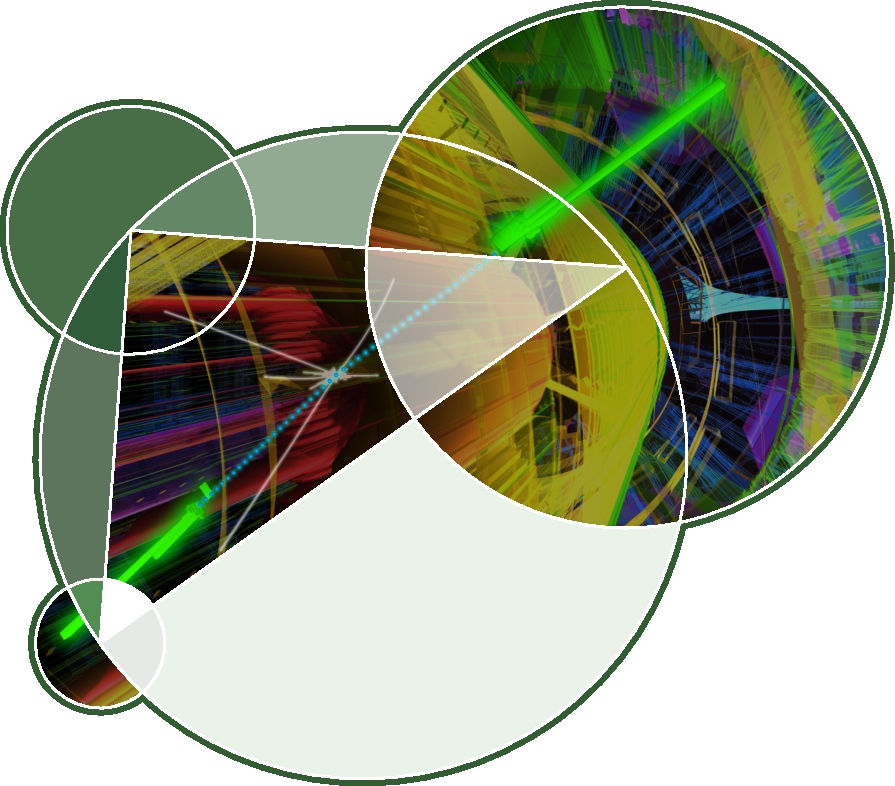
\includegraphics[height=.85\paperwidth]{figures/atlaskugrid2.pdf}}}\makebox[0pt][r]{\raisebox{3.2mm}[0pt][0pt]{\textcolor{natgreen}{\rule{.06\paperwidth}{.7pt}}}}\makebox[0pt][l]{\raisebox{3.2mm}[0pt][0pt]{\textcolor{natgreen}{\rule{.95\paperwidth}{.7pt}}}}





\bigskip

{\sffamily
\begin{hangparas}{0em}{0}
{\textbf{ }

\vspace{2em}}

{\LARGE \textbf{Master's thesis}

\vspace{.3em}}

{\Large Kristoffer Levin Hansen}

\vspace{3em}

{\Huge \raggedright
Search for new physics in diphoton production with the ATLAS detector at the LHC
}
\vfill{}

{\Large Academic advisor: Jørgen Beck Hansen}
\vspace{28em}

\today
\end{hangparas}
}
\clearpage}
\thispagestyle{empty}
  \phantom{p}
\vspace{1.16\textwidth}

\begin{center}

\includegraphics[width=.1\textwidth]{star1}

\vspace{2em}
\begin{minipage}{.6\textwidth}
\emph{``Art is never finished, merely abandoned.''}

\raggedleft\small\sffamily\bfseries\vspace{1em} -- Leonardo da Vinci
\end{minipage}
\end{center}
\clearpage
\end{titlingpage}
\frontmatter

\begin{abstract}
In this thesis, we will conduct a search for physics beyond the Standard Model by introducing into it, via the effective Lagrangian approach, a new $qq\gamma\gamma$ contract interaction. The effects of this new interaction on the distribution of invariant masses of diphotons will be assessed via the production of Monte Carlo simulations at two values of the associated mass scale $\Lambda$, and a corresponding Monte Carlo set for the Standard Model. These Monte Carlo sets will be subjected to full \atlas{} detector stimulation, before they are compared with data taken by \atlas{} during the 2012, 8 TeV run of the LHC. A fully data driven background estimation will be carried out on this data set. Finally, we will interpolate our Monte Carlo samples, so that we may compare a distribution corresponding to any $\Lambda$ with the experimental distribution. This can be used for a maximum profile likelihood fit of $\Lambda$ to data.
\end{abstract}

\end{english}
\renewcommand{\abstractname}{Resumé på dansk}
\begin{abstract}
I dette speciale vil vi søge efter ny fysik ud over Standardmodellen, ved at indføre en ny $qq\gamma\gamma$ kontaktinteraktion ved brug af en effektiv Lagrangefunktion. Vi vil undersøge effekten af en sådan ny interaktion på fordelingen af invariante masser af difotoner produceret ved protonsammenstød, ved at fremstille Monte Carlo dataset ved to værdier af den tilhørende masseskala $\Lambda$, samt et korresponderende Monte Carlo sæt for Standardmodellen. Disse Monte Carlo sæt køres igennem den fulde \atlas{} detektor simulering, før de sammenlignes med data taget af \atlas{} under 8 TeV kørslen i LHC i 2012. En fuldt datadreven baggrundsestimering vil blive udført på det eksperimentelle data sæt. Endelig vil vi interpolere vores Monte Carlo datasæt, således at vi kan sammenligne distributioner der tilsvarer enhver værdi af $\Lambda$ med den eksperimentelle distribution. På den måde kan et maksimal profil likelihood fit af $\Lambda$ til data udføres.
\end{abstract}
\begin{english}
\newpage

\tableofcontents
\mainmatter

\chapter{Introduction}

Since the late 1960s, our---at times evolving---understanding of the properties and interactions of the fundamental particles has been summarised by the Standard Model of Particle Physics. The Standard Model is formulated in the language of Quantum Field Theory\footnote{Capitalised in anticipation of the imminent use of its common abbreviation, QFT.}, and attempts to combine a theoretical model of quantum mechanical phenomena with an experimental understanding of the properties of fundamental particles and the couplings between them.

An overview of a selection of these properties and interactions is given in fig.~\ref{SMsum}.

\begin{figure}[htp]
\begin{minipage}[b]{.745\textwidth}
\begin{infilsf}
\begin{sffamily}\begin{scriptsize}
\pgfdeclarelayer{back}
\pgfsetlayers{back,main}
\begin{tikzpicture}[yscale=1.8,xscale=0.35]

\tikzstyle{quark}=[font=\footnotesize,white,circle,draw=white,fill=natgreen,inner sep=0pt,minimum size=12pt]
\tikzstyle{gauge}=[font=\footnotesize,white,circle,draw=white,fill=natcomp,inner sep=0pt,minimum size=12pt]
\tikzstyle{higgs}=[font=\footnotesize,white,circle,draw=white,fill=natyellow,inner sep=0pt,minimum size=12pt]
\tikzstyle{lepton}=[font=\footnotesize,white,circle,draw=white,fill=natblue,inner sep=0pt,minimum size=12pt]
\tikzstyle{quarko}=[fill=white,circle,draw=natgreen,inner sep=0pt,minimum size=16pt]
\tikzstyle{gaugeo}=[fill=white,circle,draw=natcomp,inner sep=0pt,minimum size=16pt]
\tikzstyle{higgso}=[fill=white,circle,draw=natyellow,inner sep=0pt,minimum size=16pt]
\tikzstyle{leptono}=[fill=white,circle,draw=natblue,inner sep=0pt,minimum size=16pt]
\tikzstyle{inter}=[kugray!50, ultra thick,cap=rect]
\tikzstyle{under}=[line width=3pt,white]

\draw (-3.5,1.8) -- (-3.5,-1.5) -- (-1.7,-1.5) [snake=zigzag] -- (-.3,-1.5) [snake=none] --  (21,-1.5) -- (21,1.8) -- cycle;
\draw (-3.5,0) node[left] {0} -- +(8pt,0);
\draw (-3.5,1) node[left] {1} -- +(8pt,0);
\draw (-3.5,-1) node[left] {-1} -- +(8pt,0);
\draw (-2,-1.5) -- +(0,2.5pt) +(0,-.9em) node[above] {0};
\foreach \x in {0,1}
\draw (\x*2.303,-1.5) -- +(0,2.5pt) 
    +(0.693,0) -- +(0.693,1.5pt) +(1.1,0) -- +(1.1,1.5pt) 
    +(1.39,0) -- +(1.39,1.5pt) +(1.61,0) -- +(1.61,1.5pt) +(1.79,0) -- +(1.79,1.5pt)
    +(1.95,0) -- +(1.95,1.5pt) +(2.08,0) -- +(2.08,1.5pt) +(2.2,0) -- +(2.2,1.5pt);
\foreach \x in {2,3,...,8}
\draw (\x*2.303,-1.5) -- +(0,2.5pt) +(0,-.9em) node[above] {$10^{\x}$}
    +(0.693,0) -- +(0.693,1.5pt) +(1.1,0) -- +(1.1,1.5pt) 
    +(1.39,0) -- +(1.39,1.5pt) +(1.61,0) -- +(1.61,1.5pt) +(1.79,0) -- +(1.79,1.5pt)
    +(1.95,0) -- +(1.95,1.5pt) +(2.08,0) -- +(2.08,1.5pt) +(2.2,0) -- +(2.2,1.5pt);
\draw (0,-1.5) -- +(0,2.5pt) +(0,-.9em) node[above] {1};
\draw (2.303,-1.5) -- +(0,2.5pt) +(0,-.9em) node[above] {10};
\draw (9*2.303,-1.5) -- +(0,2.5pt) +(0,-.9em) node[above] {$10^9$};
\node at (-4.8,1.7) [rotate=90,left] {Electromagnetic charge [e]};
\node at (21,-1.8) [left] {Mass [eV/c$^2$]};
\draw (7.74,0.667) node [quarko] (u) {} node {\tikz {\fill[natgreen] (0,0) -- ++(0,8pt) arc (90:-90:8pt) -- cycle; \draw +(180:8pt);}} node [quark] {u};
\draw (8.48,-0.333) node [quarko] (d) {} node {\tikz {\fill[natgreen] (0,0) -- ++(0,8pt) arc (90:-90:8pt) -- cycle; \draw +(180:8pt);}} node [quark] {d};
\draw (14.06,0.667) node [quarko] (s) {} node {\tikz {\fill[natgreen] (0,0) -- ++(0,8pt) arc (90:-90:8pt) -- cycle; \draw +(180:8pt);}} node [quark] {s};
\draw (11.46,-0.333) node [quarko] (c) {} node {\tikz {\fill[natgreen] (0,0) -- ++(0,8pt) arc (90:-90:8pt) -- cycle; \draw +(180:8pt);}} node [quark] {c};
\draw (18.97,0.667) node [quarko] (t) {} node {\tikz {\fill[natgreen] (0,0) -- ++(0,8pt) arc (90:-90:8pt) -- cycle; \draw +(180:8pt);}} node [quark] {t};
\draw (15.25,-0.333) node [quarko] (b) {} node {\tikz {\fill[natgreen] (0,0) -- ++(0,8pt) arc (90:-90:8pt) -- cycle; \draw +(180:8pt);}} node [quark] {b};
\draw (-2,0) ++(100:6.5pt) ++(-4.47pt,0) node (gamma) [gaugeo] {} node {\tikz {\shade[top color=white,bottom color=natcomp] (0,0)  +(-80:12pt) -- +(-45:8pt) arc (-45:-115:8pt) -- cycle; \filldraw[natcomp] (0,0) circle (8pt); \draw +(100:12pt);}} node [gauge] {$\gamma$};
\draw (-2,0) ++(-80:6.5pt) ++(4.47pt,0) node [gaugeo] (g) {} node {\tikz {\shade[top color=natcomp,bottom color=white] +(100:12pt) -- +(135:8pt) arc (135:65:8pt) -- cycle; \filldraw[natcomp] (0,0) circle (8pt); \draw +(-80:12pt);}} node [gauge] {g};
\draw (-2,0) node {\tikz \fill[natcomp] circle (1pt);};
\draw (18.33,0) ++(100:6.5pt) ++(-4.47pt,0) node [gaugeo] (Z) {} node {\tikz {\shade[top color=white,bottom color=natcomp] (0,0)  +(-80:12pt) -- +(-45:8pt) arc (-45:-115:8pt) -- cycle; \filldraw[natcomp] (0,0) circle (8pt); \draw +(100:12pt);}} node [gauge] {Z};
\draw (18.20,1) node [gaugeo] (W+) {} node {\tikz {\filldraw[natcomp] (0,0) circle (8pt);}} node [gauge] {\tiny W$^+$};
\draw (18.20,-1) node [gaugeo] (W-) {} node {\tikz {\filldraw[natcomp] (0,0) circle (8pt);}} node [gauge] {\tiny W$^-$};
\draw (18.65,0)  ++(-80:6.5pt) ++(4.47pt,0) node [higgso] (H) {} node {\tikz {\shade[top color=natyellow,bottom color=white] +(100:12pt) -- +(135:8pt) arc (135:65:8pt) -- cycle; \draw +(-80:12pt); \draw[natyellow] (0,0) circle (8pt);}} node [higgs] {H};
\draw (18.33,0) node {\tikz \fill[natcomp] circle (1pt);};
\draw (18.65,0) node {\tikz \fill[natyellow] circle (1pt);};
\draw (0.79,0) node [leptono] (ve) {} node {\tikz {\fill[natblue] (0,0) -- ++(0,8pt) arc (90:-90:8pt) -- cycle; \draw +(180:8pt);}} node [lepton] {$\nu_{\text e}$};
\draw (5.14,0) node [leptono] (vmu) {} node {\tikz {\fill[natblue] (0,0) -- ++(0,8pt) arc (90:-90:8pt) -- cycle; \draw +(180:8pt);}} node [lepton] {$\nu_\mu$};
\draw (9.65,0) node [leptono] (vtau) {} node {\tikz {\fill[natblue] (0,0) -- ++(0,8pt) arc (90:-90:8pt) -- cycle; \draw +(180:8pt);}} node [lepton] {$\nu_\tau$};
\draw (6.24,-1) node [leptono] (e) {} node {\tikz {\fill[natblue] (0,0) -- ++(0,8pt) arc (90:-90:8pt) -- cycle; \draw +(180:8pt);}} node [lepton] {e};
\draw (11.57,-1) node [leptono] (mu) {} node {\tikz {\fill[natblue] (0,0) -- ++(0,8pt) arc (90:-90:8pt) -- cycle; \draw +(180:8pt);}} node [lepton] {$\mu$};
\draw (14.39,-1) node [leptono] (tau) {} node {\tikz {\fill[natblue] (0,0) -- ++(0,8pt) arc (90:-90:8pt) -- cycle; \draw +(180:8pt);}} node [lepton] {$\tau$};

\begin{pgfonlayer}{back}
\node at (12,1) [inner sep=0] (uqs) {};
\node at (20.7,.6) [inner sep=0] (qgnode) {};
\draw [inter] (u) to[out=0,in=270,max distance=7pt]  (uqs);
\draw [inter] (s) to[out=170,in=270,max distance=4pt] (uqs);
\draw [inter] (t) to[out=190,in=270,max distance=25pt] (uqs);
\draw [inter] (d) to[out=5,in=270,max distance=30pt] (uqs);
\draw [inter] (c) to[out=60,in=270,max distance=10pt] (uqs);
\draw [inter] (b) to[out=170,in=270,max distance=20pt] (uqs)
                  to[out=90,in=40,max distance=17pt] (g);
\draw (g) node[below right] {\tikz {\draw [inter] (0,0) to[in=-40,out=-90,min distance=20pt] (0,0);}};
\draw [inter] (uqs) to[out=90,in=30,max distance=15pt] (gamma);
\draw [inter] (uqs) to[out=90,in=150,max distance=7pt] (W+);
\draw [inter] (uqs) .. controls (12,1.4) and (20.7,1.7) .. (qgnode.south)
                    to[out=270,in=10,max distance=7pt] (Z);
\draw [inter] (qgnode) to[out=270,in=20,max distance=10pt] (H);
\draw [inter] (qgnode) to[out=270,in=20,max distance=30pt] (W-);

\draw [under] (gamma) -- ++(15,0) node [inner sep=0] (gamw) {};
\draw [under] (gamw.west) to[out=0,in=90,max distance=30pt] (W-);
\draw [under] (gamw.west) to[out=0,in=250,max distance=20pt] (W+);
\draw [inter] (gamma) -- (gamw.east);
\draw [inter] (gamw.west) to[out=0,in=250,max distance=20pt] (W+);
\draw [inter] (gamw.west) to[out=0,in=90,max distance=30pt] (W-);

\node at (17,-.3) [inner sep=0] (wz-) {};
\node at (17,.6) [inner sep=0] (wz+) {};
\draw [under] (wz-) -- (wz+) to[out=270,in=160,max distance=10pt] (Z);
\draw [under] (H) to[out=30,in=-5,min distance=30pt] (W+);
\draw [inter] (W-) to[out=160,in=270,max distance=10pt] (wz-)
           to (wz+.north) to[out=90,in=200,max distance=10pt] (W+);
\node [above right] at (W+) {\tikz {
    \draw[under] (0,0) to[out=40,in=90,min distance=20pt] (0,0);
    \draw[inter] (0,0) to[out=40,in=90,min distance=20pt] (0,0);}};
\draw [inter] (wz-) to[out=90,in=200,max distance=10pt] (Z);
\draw [inter] (wz+) to[out=270,in=160,max distance=10pt] (Z);
\draw [inter] (W-) -- (H);
\draw (W-) node[below right] {\tikz {\draw [inter] (0,0) to[in=-40,out=-90,min distance=20pt] (0,0);}};
\draw [inter] (H) to[out=50,in=-10,max distance=5pt] (Z);
\draw [inter] (H) to[out=30,in=-5,min distance=30pt] (W+);

\draw (tau) ++(1.5,.25) node [inner sep=0] (lepga) {};
\draw [inter] (tau) to[out=70,in=180,max distance=3pt] (lepga)
                    to[out=0,in=270,max distance=10pt] (wz-);
\draw [inter] (mu) to[out=70,in=180,max distance=3pt] ++(1.5,.25) -- (lepga);
\draw [inter] (e) to[out=70,in=180,max distance=3pt] ++(1.5,.25)
              node [inner sep=0] (ega) {} -- (lepga);
\draw [inter] (lepga) to[out=0,in=152,max distance=10pt] (W-);

\draw (vmu) ++(-1.5,-.25) node [inner sep=0] (neul) {};
\draw [inter] (vmu) to[out=250,in=0,max distance=3pt] (neul);
\draw [inter] (vtau) to[out=185,in=0,min distance = 30pt] (neul);
\draw [inter] (ve) -- ++(0,-.5) node [inner sep=0] (neud) {};
\draw [inter] (neul.east) to[out=180,in=90,max distance=7pt] (neud);
\draw [inter] (neud.north) to [out=270,in=180,max distance=10pt] (ega);

\draw (g) ++(-1,0) node [inner sep=0] (gamlep) {};
\draw [inter] (e) to [out=250,in=0,max distance=3pt] ++(-1.5,-.25)
              node (lepneu) [inner sep=0] {};
\draw [inter] (mu) to[out=250,in=0,max distance=3pt] ++(-1.5,-.25) -- (lepneu);
\draw [inter] (tau) to[out=250,in=0,max distance=3pt] ++(-1.5,-.25) -- (lepneu);
\draw [inter] (lepneu.east) to[out=180,in=270,max distance=20pt] (neud.north);
\draw [inter] (lepneu) to[out=180,in=270,max distance=30pt] (gamlep);
\draw [inter] (gamma) to[out=230,in=90] (gamlep.south);
\end{pgfonlayer}

\draw[inter,cap=round] (-2,1) -- (0,1) node[right,kugray] {Interactions};

\draw (-1,1.4) node [quarko] (n) {} node {\tikz {\fill[natgreen] (0,0) -- ++(0,8pt) arc (90:-90:8pt) -- cycle; \draw +(180:8pt);}} node [quark] {n};
\node at (n) {\tikz {\draw [white,postaction={decorate,decoration={text along path,text align=center,text={|\tiny|Spin}}}] ++(270:10pt) arc (270:90:10pt); \draw (-1,0) (1,0);}};
\begin{scope}
\clip (n.center) -- ++(2,0) -- ++(0,.2) -- ++(-2,0) -- cycle;
\draw (n) node [gaugeo] {} node {\tikz {\filldraw[natcomp] (0,0) circle (8pt);}} node [gauge] {n};
\end{scope}
\begin{scope}
\clip (n.center) -- ++(2,0) -- ++(0,-.2) -- ++(-2,0) -- cycle;
\draw (n) node [leptono] {} node {\tikz {\fill[natblue] (0,0) -- ++(0,8pt) arc (90:-90:8pt) -- cycle; \draw +(180:8pt);}} node [lepton] {n};
\end{scope}
\begin{scope}
\clip (n.center) -- ++(-2,0) -- ++(0,-.2) -- ++(2,0) -- cycle;
\draw (n) node [higgso] {} node {\tikz {\shade[top color=natyellow,bottom color=white] +(100:12pt) -- +(135:8pt) arc (135:65:8pt) -- cycle; \draw +(-80:12pt); \draw[natyellow] (0,0) circle (8pt);}} node [higgs] {n};
\end{scope}

\draw (n) ++(160:20pt) node [right,natgreen] {\tiny Quarks};
\draw (n) ++(-160:20pt) node [right,natyellow] {\tiny Higgs boson};
\draw (n) ++(0:20pt) node [above right,natcomp] {\tiny Gauge bosons};
\draw (n) ++(0:20pt) node [below right,natblue] {\tiny Leptons};

\end{tikzpicture}
\end{scriptsize}\end{sffamily}
\end{infilsf}
\end{minipage}
\hfill\begin{minipage}[b]{.25\textwidth}
\caption{An overview of the particles of the Standard Model. The particles are arranged by mass and charge. Colour indicates particle type, the filling of the border indicates the spin of particles and lines are drawn between those particles that the Standard Model describes interactions between. The currently known maximum bounds on neutrino masses have been used to place the neutrinos in the mass direction. Table values from \cite{wikism}.\label{SMsum}}
\end{minipage}
\end{figure}

In its current form, the Standard Model makes no attempt to explain any physics beyond this.\footnote{The overview in figure~\ref{SMsum} includes massive neutrinos, which have been found experimentally, even though the Standard Model does not at present include them. There are, however, several proposed methods of extending the SM to do so.} The most obvious missing element is gravity, which finds no obvious expression in terms of Quantum Field Theory. Other seemingly missing elements come from astronomy, which bring observational evidence of a number of phenomena, such as dark matter and dark energy, which seem to require an explanation from within the realm of physics that the Standard Model describes, but for which the Standard Model offers no obvious source.

Disregarding these issues, which may be considered external its scope, the Standard Model has been remarkably successful as a model for high energy particle physics, withstanding decades of experimental tests and correctly predicting the existence and properties of several particles.\footnote{Most recently, the existence of the Higgs boson was confirmed experimentally. At the time of writing, confirmation of its predicted properties is still a work in progress.} In spite of those successes, the Standard Model is not without its issues.

As it is formulated, the SM depends on at least 19 numerical constants,\footnote{Not counting any additional constants needed to account for neutrino masses.} the value of which must be determined experimentally, since the model offers no insight into the origin of or relations between them. Worse still, as the SM is a perturbative model, higher order corrections, which tend to increase the predicted Higgs mass with no constraint save the Planck energy, must be included in the theory. To arrive at the observed Higgs mass in spite of this tendency, either some unknown physics exist between the Higgs mass scale and the Planck scale to constrain the Higgs mass, or the bare mass and couplings of the Higgs boson are very finely tuned to cancel the higher order contributions. This is one example of the hierarchy problem.

In the first case, we will obviously want to search for evidence of the postulated new, high-energy physics. In the latter case, we might expect\footnote{Or \emph{hope for}, depending on how invested we happen to be in the question of fine--tuning.} there to be some additional mechanism within the Standard Model that ensures that the bare Higgs mass and the other free parameters of the SM are given the proper value. Again, we will want to search for physics outside what is currently described by the SM, as a clue to what that mechanism might be.

There is also the possibility that neither of those mechanisms exist, since the Standard Model, strictly speaking, does not require them. In that case a search for new physics that discovers nothing is still a valuable, albeit less illuminating, result.

In this thesis, we shall approach the task of searching for physics beyond the Standard Model by introducing to it an extension via the effective Lagrangian approach. Specifically, we will introduce a $q\bar q\rightarrow\gamma\gamma$ point interaction, and then simulate collision experiments with the new interaction at various strengths, to see how the outcome is affected. We can then, finally, compare the results of those pseudoexperiments to the results of actual collision experiments performed at \textsc{cern}'s Large Hadron Collider, and look for signs of the same effects there.

\chapter{Theory}\label{ch.theory}

While the detailed procedure for going from a general notion of expanding the Standard Model to creating a specific set of pseudoexperiments with which to compare experimental results are not part of the main thrust of this thesis, and will in any case be handled by various software tools in practice, what will follow is a brief overview of that process.

Since the new interaction will be introduced into the SM by the effective Lagrangian approach, the Lagrangian formulation of the Standard Model as a quantum field theory will be the starting point.

\section{The Lagrangian formulation of QFT}
In classical mechanics \cite{goldstein}, the Lagrangian formulation describes the path taken by a system between a given initial and final state---a particle with an initial and a final position, say---by finding the path between these states that minimises the action $S$, which is defined as the integral along a given path over the Lagrangian $L$:
\[S[q]=\int_\textrm{path}dtL[q,\dot{q}],\]
where $q$ is a generalised coordinate. In this picture, the Lagrangian encapsulates the dynamics of the system. It is related to the Hamiltonian $H$ by
\(L = p\dot q- H,\label{htol}\)
where $p$ is momentum.

In quantum mechanics, the picture of a system travelling along a single, well-defined path from an initial to a final configuration no longer applies. In stead, a probability of going from an initial state $\ket{q}$ to a final state $\ket{q\prime}$ can be found as the absolute square of the transition amplitude\footnote{At this point, we should note that the common notation where $\hbar = c = 1$ will be used from this chapter onwards.} \cite{srednicki}
\[A=\bra{q\prime}e^{-i\hat H(t\prime-t)}\ket{q\phantom\prime},\]
where $\hat H$ is the Hamiltonian of the system. Since the idea of a singular path for the system was abandoned, in stead imagine the system travelling along each possible path simultaneously, each with its own transition amplitude. The total transition amplitude, then, is the sum of all the individual transition amplitudes. This can be connected to the classical case by supposing that, for a system with a classical limit, the transition amplitudes of paths close to the classical path will tend to amplify one another, while paths far from it will tend to cancel out.

Through some notational gymnastics, which involve carving the path integral into an infinite number of time steps, each integrated over every possible configuration, and imposing some conditions on the Lagrangian, it can be shown \cite{srednicki} that the expression above can be written as
\(A=\int\,\mathcal Dq\,\exp\left[i\int_t^{t^\prime}dt\,[p(t)\dot q(t)-H(p(t),q(t))]\right],\label{e.Dq}\)
where the integral is over all paths with position $q$ at time $t$ and position $q\prime$ at time $t\prime$. We recognise the expression in the innermost integral from eq.~\eqref{htol}.

For a local theory, it is possible to write the Lagrangian as a spatial integral over the Lagrangian density:
\[L=\int \,d^3x\,\mathcal L.\]
Thus, the action can be written as
\(S=\int\,d^4x\,\mathcal L,\label{e.S}\)
which, unlike the previous expression for $S$, is manifestly Lorenz invariant, so long as $\mathcal L$ is a Lorenz scalar. Given the ubiquity of local quantum field theories, it is common when discussing quantum field theory to drop `density' from the name, and refer to $\mathcal L$ as the Lagrangian. Going forward, we will also follow that convention here.

Finally, to get the field theory aspect, replace the generalised coordinate $q$ with a field configuration ``coordinate'' $\phi(x)$, which depends on the Lorenz vector $x$. In short, \eqref{e.Dq} can then be written as
\(A=\int\mathcal D\phi\, e^{iS[\phi]}.\label{e.Dphi}\)

As was the case in classical mechanics, the behaviour of a theory is fully described by its Lagrangian (density), and several models can be combined by adding together their respective Lagrangians. So it is that the Standard Model is described by the SM Lagrangian $\mathcal L_{SM}$, which can be considered as a sum of several lesser Lagrangians that describe the separate sectors of the SM. However, before we venture too deeply into the Standard Model, we shall first consider an alternate way of looking at the content of the Lagrangian.

\section{The Standard Model Lagrangian}

The Lagrangian which describes the Standard Model, denoted $\mathcal{L}_{\text{\emph{SM}}}$, can, then, be considered a sum of a series of lesser Lagrangians. $\mathcal{L}_{\text{\emph{SM}}}$ can be divided into sectors in several ways, according to the needs of the author \cite{srednicki,wikism}. For this work, the sectors of the Standard Model shall be defined as follows,
\[\mathcal{L}_{\text{\emph{SM}}}=\mathcal{L}_{\text{\emph{EW}}}+\mathcal{L}_{\text{\emph{QCD}}}+\mathcal{L}_{H},\]
into sectors describing the electroweak part $\mathcal{L}_{\text{\emph{EW}}}$, the QuantumChromoDynamics part $\mathcal{L}_{\text{\emph{QCD}}}$ and the Higgs part $\mathcal{L}_{\text{\emph{H}}}$.

The electroweak Lagrangian can be expanded to read as follows:
\[\mathcal{L}_\text{\emph{EW}}=-\ono4W^i_{\mu\nu}W_i^{\mu\nu}-\ono4B_{\mu\nu}B^{\mu\nu}+\sum_\psi\bar\psi\gamma^\mu \left(i\partial_\mu-{1\over2}g^\prime Y_\mathrm{W}B_\mu-{1\over2}g\sigma^a W^a_\mu\right)\psi,\]
where $W^i_{\mu}$ and $B_{\mu}$ are the four ($i$ runs from 1 to 3) gauge fields of electroweak theory and $W^i_{\mu\nu}$ and $B_{\mu\nu}$ are their field strength tensors, the $\phi$ sum is over all left--handed fermionic (lepton and quark) fields, $\gamma_{\mu}$ is the Dirac matrices, $g$ and $g'$ are the coupling strengths of the theory, $Y_W$ is the weak hypercharge associated with the fermionic field and $\sigma_i$ are the Pauli matrices. The terms for right--handed fermions have been omitted.

The physical $W^\pm_\mu$, $Z^0_\mu$ and $A_\mu$ fields, which manifest as the W and Z bosons and the photon, respectively, arise as mixtures of the gauge fields:
\(\begin{aligned}
W_\mu^\pm&=\ono{\sqrt{2}} W^1_\mu\mp iW^2_\mu\\
Z^0_\mu&=W^3_\mu\cos \theta_W-B_\mu\sin \theta_W\\
A_\mu&=W^3_\mu\sin\theta_W+B_\mu\cos\theta_W,
\end{aligned}\label{tophys}\)
where $\theta_W$ is the Weinberg mixing angle, an empirically determined parameter of the model. It also relates the coupling strengths to the electromagnetic coupling constant $e$ though
\[e=g'\cos\theta_W=g\sin\theta_W.\]

Applying the relations in eqs.~\eqref{tophys} allows us to rewrite $\mathcal{L}_{\text{\emph{EW}}}$ to a form that depends solely on these physical fields. Focusing on terms that depend on
\[F_{\mu\nu}=\partial_\mu A_\nu - \partial_\nu A_\mu,\]
the electromagnetic field strength tensor, that come from just the first two terms in $\mathcal{L}_{\text{\emph{EW}}}$, produces
\(\mathcal{L}_{\text{\emph{EW}}}=-\ono4 F^{\mu\nu}F_{\mu\nu}+ie F^{\mu\nu}W^{+}_\mu W^{-}_\nu+\cdots\label{ewfmn}\)
The first of these terms describes the propagation of the $A_\mu$ field from one configuration to another, or, in more immediate terms, the propagation of photons through space. Fourier--transforming to momentum space allows us to write the action for this term as
\(S_{\textit{EW}}=-\ono2\int\frac{d^4k}{(2\pi)^4}\tilde A_\mu(k)k^2\tilde A_\nu(-k)+\cdots,\)
implying that the photon propagator in momentum space is
\(\Delta(k)=\ono{k^2-i\epsilon},\label{phoprop}\)
assuming that momentum conservation is imposed. Here, the modification of the denominator by $i\epsilon$ is included to avoid the pole at $k=0$. This particular way of dealing with poles in the integration of the propagators is due to Richard Feynman, making this the Feynman propagator.

Also due to Richard Feynman is the notion that the terms in the Lagrangian can be represented graphically.

\section{Feynman diagrams}
We represent the photon propagator given in eq.~\eqref{phoprop} graphically as shown in fig.~\ref{phoprop}.

\begin{figure}[hbtp]
\begin{minipage}[c]{.69\textwidth}\centering\footnotesize
\begin{tikzpicture}
\draw[decorate, decoration={snake}] (0,0) -- node[midway,above] {$\gamma$} (2,0) ;
\node[right] at (3,0) {$ = \dfrac{1}{k^2-i\epsilon}$};
\end{tikzpicture}
\end{minipage}\hfill
\begin{minipage}[c]{.3\textwidth}
\caption{Feynman rule for the photon propagator.}
\label{phoprop}
\end{minipage}
\end{figure}

The second term in eq.~\eqref{ewfmn} describes an interaction between the photon and the $W$ bosons, the graphical representation of which is given in fig.~\ref{wwgam}.

\begin{figure}[htbp]
\begin{minipage}[b]{.69\textwidth}\centering\footnotesize
\begin{tikzpicture}
\draw[decorate, decoration={snake, pre=lineto, pre length=5pt}] (0,0) -- +(1.5,0) node[right] {$\gamma$};
\draw[decorate, decoration={snake, pre=lineto, pre length=5pt}](0,0) -- +(240:1.5) node[left] {$W^{+}$};
\draw[decorate, decoration={snake, pre=lineto, pre length=5pt}](0,0) -- +(120:1.5) node[left] {$W^{-}$};
\node[right] at (3,0) {$= ie$};
\end{tikzpicture}
\end{minipage}\hfill
\begin{minipage}[b]{.3\textwidth}
\caption{Feynman rule for the $\gamma W^{+}W^{-}$ coupling.}
\label{wwgam}
\end{minipage}
\end{figure}

The full propagators for the remaining fields require the introduction of the Higgs Lagrangian, which gives the mass terms for those fields. The relevant terms from the Higgs Lagrangian, in terms of physical fields, as given in eq.~\eqref{tophys}, to get the terms
\(\mathcal{L}_H=-\frac{g^2v^2}{4}W^{+\mu}W^{-}_\mu-\frac{g^2v^2}{8\cos\theta_W}Z^\mu Z_\mu,\)
where $v/\sqrt{2}$ is the vacuum expectation value of the Higgs field, given the correct Gauge transformation. From this, we identify the mass terms
\(m_W=\frac{g^2v^2}{2},\qquad m_Z=m_W\cos\theta_W.\)

Including the mass terms in the action for, say, a free Z boson and Fourier--transforming gives us
\[S_Z=?\int\frac{d^4k}{(2\pi)^4}\tilde Z_\mu(k)[k^2-m^2]\tilde Z\nu(-k) +\cdots,\]
leading to the more general form of the Feynman propagator,
\(\Delta(k)=\ono{k^2-m^2-i\epsilon},\)
which is the factor associated with the remaining electroweak propagators, and the Higgs propagator, which are drawn as shown in figure~\ref{ewprops}, along with the gluon propagator produced by $\mathcal{L}_\textit{QCD}$, for completeness.

\begin{figure}[hbtp]
\begin{minipage}[b]{.69\textwidth}
\centering\footnotesize
\begin{tikzpicture}
\draw[decorate, decoration={snake}] (0,0) -- node[above] {$\gamma$ / $Z^0$ / $W^\pm$} (2,0);
\end{tikzpicture}
\hspace{5em}
\begin{tikzpicture}
\draw (0,0) -- node[midway] {\tikz\draw[-triangle 45] (0,0) -- (.1,0);} node[midway,above] {$\ell$ / $\nu$ / $q$} (2,0);
\end{tikzpicture}
\vspace{1em}

\begin{tikzpicture}
\draw[dashed] (0,0) -- node[above] {$h$} (2,0);
\end{tikzpicture}
\hspace{5em}
\begin{tikzpicture}
\draw[decorate, decoration={coil,amplitude=2pt, segment length=2.68pt}] (0,0) -- node[above] {$g$} (2,0);
\end{tikzpicture}
\end{minipage}
\hfill
\begin{minipage}[b]{.3\textwidth}
\caption{Showing how line shapes and SM particles are associated.}\label{ewprops}
\end{minipage}
\end{figure}

In fig.~\ref{ewprops}, the notion that antiparticles are time--reversed particles is introduced, as indicated by the direction of the arrows.

The remainder of $\mathcal{L}_\textit{EW}$ gives rise to couplings of the types shown in fig.~\ref{restew}. For brevety, we do not show a complete listing of Feynman rules, only a condensed overview of possible vertices. For a complete listing, see eg. \cite{allfeynrules}. The couplings introduced by the QCD and Higgs sectors are given in figure~\ref{othercoups}.

\begin{figure}[hbtp]\centering {\footnotesize
\begin{tikzpicture}
\draw[decorate, decoration={snake, pre=lineto, pre length=5pt}] (0,0) -- +(1.5,0) node[right] {$Z$};
\draw[decorate, decoration={snake, pre=lineto, pre length=5pt}](0,0) -- +(240:1.5) node[left] {$W^{+}$};
\draw[decorate, decoration={snake, pre=lineto, pre length=5pt}](0,0) -- +(120:1.5) node[left] {$W^{-}$};
\end{tikzpicture}\hspace{2em}
\begin{tikzpicture}
\draw[decorate, decoration={snake, pre=lineto, pre length=5pt}] (0,0) -- +(1.5,0) node[right] {$Z/\gamma$};
\draw[](0,0) -- node[midway,sloped] {\tikz\draw[-triangle 45] (0,0)--(-.1,0);} +(240:1.5) node[left] {$f$};
\draw[](0,0) -- node[midway,sloped] {\tikz\draw[-triangle 45] (0,0)--(.1,0);} +(120:1.5) node[left] {$f$};
\end{tikzpicture}\hspace{2em}
\begin{tikzpicture}
\draw[decorate, decoration={snake, pre=lineto, pre length=5pt}] (0,0) -- +(1.5,0) node[right] {$W^\pm$};
\draw[](0,0) -- node[midway,sloped] {\tikz\draw[-triangle 45] (0,0)--(-.1,0);} +(240:1.5) node[above left] {$\nu,\ell$};
\draw[](0,0) -- node[midway,sloped] {\tikz\draw[-triangle 45] (0,0)--(.1,0);} +(120:1.5) node[above left] {$\ell,\nu$};
\draw (0,0) +(240:1.5) node[below left] {$u,d$} (0,0) +(120:1.5) node[below left] {$d,u$};
\end{tikzpicture}\hspace{2em}
\begin{tikzpicture}
\draw[decorate, decoration={snake, pre=lineto, pre length=5pt}](0,0) -- (-1.5,1) node[left] {$W^{+}$};
\draw[decorate, decoration={snake, pre=lineto, pre length=5pt}](0,0) -- (-1.5,-1) node[left] {$W^{-}$};
\draw[decorate, decoration={snake, pre=lineto, pre length=5pt}](0,0) -- (1.5,1) node[right] {$B$};
\draw[decorate, decoration={snake, pre=lineto, pre length=5pt}](0,0) -- (1.5,-1) node[right] {$B$};
\end{tikzpicture}\hspace{2em}
}
%\begin{tikzpicture}
%\draw[decorate, decoration={snake, pre=lineto, pre length=5pt}](0,0) -- node[above] {$B$} %(2,0);
%\end{tikzpicture}

\caption{The Feynman rules of the electroweak Lagrangian, excluding those given in figures \ref{phoprop} and \ref{wwgam}. Here, $B$ may be any electroweak boson ($\gamma$, $Z^0$ or $W^{\pm}$, so long as charge is conserved. $f$ is any fermion, respecting that photons only couple to electrically charged fermions and $\ell,\nu,u,d$ are lepton--neutrino or up--type---down--type quark sets.} \label{restew}
\end{figure}

An advantage of representing the terms of the Lagrangian in this way is that it allows an easy identification and organisation of possible processes, and subsequently deduction of the action that governs the associated transition amplitude. This is because Feynman diagrams are required to conserve momentum and quantum numbers, and each of the elements of a Feynman diagram are directly associated with an element of the governing equation through Feynman rules, such as were given in fig.~\ref{phoprop} and \ref{wwgam}.

For example, with the $f\bar f \rightarrow \gamma$ and the $q$ propagator already introduced, we may assemble the Feynman diagram in fig.~\ref{bornqq2gg} for a $q\bar q \rightarrow \gamma\gamma$ process.

\begin{figure}[hbtp]
\begin{minipage}[b]{.69\textwidth}
\begin{center}\begin{footnotesize}
\begin{tikzpicture} [>=triangle 45]
\draw[>-] (-1,1) -- (0,1);
\draw[->] (0,1) -- (0,0);
\draw[<-] (-1,-1) -- (0,-1) -- (0,0);
\draw (-2,1) node[left] {$q$} -- (-1,1);
\draw (-2,-1)  node[left] {$\bar q$} -- (-1,-1);
\draw[snake=coil,segment aspect=0] (0,1) -- (2,1) node[right] {$\gamma$};
\draw[snake=coil,segment aspect=0] (0,-1) -- (2,-1) node[right] {$\gamma$}; 
\end{tikzpicture}
\end{footnotesize}\end{center}
\end{minipage}\hfill
\begin{minipage}[b]{.3\textwidth}
\caption{A Feynman diagram for a $q\bar q \rightarrow \gamma\gamma$ process.}\label{bornqq2gg}
\end{minipage}
\end{figure}

To evaluate this diagram, we require the Feynman rule for the $f\bar f \rightarrow \gamma$ vertex, given in fig.~\ref{ruleqqgam}

\begin{figure}[hbtp]
\begin{minipage}[b]{.69\textwidth}
\centering\footnotesize
\begin{tikzpicture}
\draw[decorate, decoration={snake, pre=lineto, pre length=5pt}] (0,0) -- +(1,0) node[right] {$\gamma$};
\draw[](0,0) -- node[midway,sloped] {\tikz\draw[-triangle 45] (0,0)--(-.1,0);} +(240:1) node[left] {$f$};
\draw[](0,0) -- node[midway,sloped] {\tikz\draw[-triangle 45] (0,0)--(.1,0);} +(120:1) node[left] {$f$};
\node[right] at (2,0) {$=eQ_f\gamma^\mu$};
\end{tikzpicture}
\end{minipage}\hfill
\begin{minipage}[b]{.3\textwidth}
\caption{Feynman rule for the fermion--fermion--photon coupling. $e$ is the unit charge and $Q_f$ is the charge of the fermion.}\label{ruleqqgam}
\end{minipage}
\end{figure}

The Feynman diagram in fig.~\ref{bornqq2gg} is then equivalent to
\(\frac{e^2Q_q^2\gamma^\mu\gamma^\nu}{k^2-m^2-i\epsilon},\)
where $k$ is the momentum of the internal quark propagator. This relates to the transition amplitude by integrating over all participating momenta, keeping in mind that momenta must be conserved across all propagators and in every vertex.

The couplings introduced by the QCD and Higgs sectors are given in figure~\ref{othercoups}.

\begin{figure}[htbp]
\centering\footnotesize
\begin{tikzpicture}
\draw[decorate, decoration={coil,amplitude=2pt, segment length=2.68pt, pre=lineto, pre length=5pt}] (0,0) -- +(1.5,0) node[right] {$g$};
\draw[](0,0) -- node[midway,sloped] {\tikz\draw[-triangle 45] (0,0)--(-.1,0);} +(240:1.5) node[left] {$q$};
\draw[](0,0) -- node[midway,sloped] {\tikz\draw[-triangle 45] (0,0)--(.1,0);} +(120:1.5) node[left] {$q$};
\end{tikzpicture}\hspace{2em}
\begin{tikzpicture}
\draw[decorate, decoration={coil,amplitude=2pt, segment length=2.68pt, pre=lineto, pre length=5pt}] (0,0) -- +(1.5,0) node[right] {$g$};
\draw[decorate, decoration={coil,amplitude=2pt, segment length=2.68pt, pre=lineto, pre length=5pt}](0,0) -- +(240:1.5) node[left] {$g$};
\draw[decorate, decoration={coil,amplitude=2pt, segment length=2.68pt, pre=lineto, pre length=5pt}](0,0) -- +(120:1.5) node[left] {$g$};
\end{tikzpicture}\hspace{2em}
\begin{tikzpicture}
\draw[decorate, decoration={coil,amplitude=2pt, segment length=2.68pt, pre=lineto, pre length=5pt}](0,0) -- (-1.5,1) node[left] {$g$};
\draw[decorate, decoration={coil,amplitude=2pt, segment length=2.68pt, pre=lineto, pre length=5pt}](0,0) -- (-1.5,-1) node[left] {$g$};
\draw[decorate, decoration={coil,amplitude=2pt, segment length=2.68pt, pre=lineto, pre length=5pt}](0,0) -- (1.5,1) node[right] {$g$};
\draw[decorate, decoration={coil,amplitude=2pt, segment length=2.68pt, pre=lineto, pre length=5pt}](0,0) -- (1.5,-1) node[right] {$g$};
\end{tikzpicture}\hspace{2em}
\begin{tikzpicture}
\draw[dashed] (0,0) -- +(1.5,0) node[right] {$h$};
\draw[](0,0) -- node[midway,sloped] {\tikz\draw[-triangle 45] (0,0)--(-.1,0);} +(240:1.5) node[left] {$f$};
\draw[](0,0) -- node[midway,sloped] {\tikz\draw[-triangle 45] (0,0)--(.1,0);} +(120:1.5) node[left] {$f$};
\end{tikzpicture}\hspace{2em}
\begin{tikzpicture}
\draw[dashed] (0,0) -- +(1.5,0) node[right] {$h$};
\draw[decorate, decoration={snake, pre=lineto, pre length=5pt}](0,0) -- +(240:1.5) node[left] {$Z^0$ / $W^\pm$};
\draw[decorate, decoration={snake, pre=lineto, pre length=5pt}](0,0) -- +(120:1.5) node[left] {$Z^0$ / $W^\mp$};
\end{tikzpicture}\hspace{2em}
\begin{tikzpicture}
\draw[dashed] (0,0) -- +(1.5,0) node[right] {$h$};
\draw[dashed](0,0) -- +(240:1.5) node[left] {$h$};
\draw[dashed](0,0) -- +(120:1.5) node[left] {$h$};
\end{tikzpicture}\hspace{2em}
\begin{tikzpicture}
\draw[decorate, decoration={snake, pre=lineto, pre length=5pt}](0,0) -- (-1.5,1) node[left] {$Z^0$ / $W^\pm$};
\draw[decorate, decoration={snake, pre=lineto, pre length=5pt}](0,0) -- (-1.5,-1) node[left] {$Z^0$ / $W^\pm$};
\draw[dashed](0,0) -- (1.5,1) node[right] {$h$};
\draw[dashed](0,0) -- (1.5,-1) node[right] {$h$};
\end{tikzpicture}\hspace{2em}
\begin{tikzpicture}
\draw[dashed](0,0) -- (-1.5,1) node[left] {$h$};
\draw[dashed](0,0) -- (-1.5,-1) node[left] {$h$};
\draw[dashed](0,0) -- (1.5,1) node[right] {$h$};
\draw[dashed](0,0) -- (1.5,-1) node[right] {$h$};
\end{tikzpicture}\hspace{2em}
\caption{Couplings introduced in $\mathcal{L}_\textit{QCD}$ and $\mathcal{L}_H$.}\label{othercoups}
\end{figure}

With these couplings in the mix, we can additionally construct the diagrams with $\gamma\gamma$ final states in figure~\ref{hiorder}.

\begin{figure}[hbtp]
\begin{minipage}[b]{.49\textwidth}
\begin{center}\begin{footnotesize}
\begin{tikzpicture} [>=triangle 45,scale=.8]
\draw[>-] (1,1) node[below]{$q$} -- (2,1);
\draw[decorate, decoration={coil,amplitude=2pt, segment length=2.68pt}] 
    (-2,1) node[left]{$g$} -- (0,1) ;
\draw[decorate, decoration={coil,amplitude=2pt, segment length=2.68pt}] 
    (-2,-1) node[left]{$g$} -- (0,-1); 
\draw[<-] (1,-1) node[above]{$\bar q$} -- (2,-1);
\draw (0,1) -- (1,1);
\draw (0,-1) -- (1,-1);
\draw[-<] (0,1) -- (0,0);
\draw (0,0) -- (0,-1);
\draw[->] (2,1) -- (2,0);
\draw (2,0) -- (2,-1);
\draw[decorate, decoration={snake}] (2,1) -- (4,1) node[right]{$\gamma$};
\draw[decorate, decoration={snake}] (2,-1) -- (4,-1) node[right]{$\gamma$};
\end{tikzpicture}
\end{footnotesize}\end{center}
\end{minipage}\hfill
\begin{minipage}[b]{.49\textwidth}
\centering\footnotesize
\begin{tikzpicture}[scale=.7]
\draw[dashed] (0,0) node[left] {$h$} -- (2,0);
\draw (2,0) -- node[midway,sloped] {\tikz\draw[-triangle 45] (0,0)--(.1,0);} (4,1) --
    node[midway,sloped] {\tikz\draw[-triangle 45] (0,0)--(.1,0);} (4,-1) --
    node[midway,sloped] {\tikz\draw[-triangle 45] (0,0)--(.1,0);} (2,0);
\node at (3.3,0) {$f$};
\draw[decorate, decoration={snake, pre=lineto, pre length=5pt}] (4,1) -- (6,1) node[right] {$\gamma$};
\draw[decorate, decoration={snake, pre=lineto, pre length=5pt}] (4,-1) -- (6,-1) node[right] {$\gamma$};
\end{tikzpicture}
\end{minipage}
\caption{Single loop level Feynman diagrams with $\gamma\gamma$ final states.}\label{hiorder}
\end{figure}

Both these diagrams introduce a new complication, in that the internal loops contain a momentum which is not fixed by momentum conservation in the vertices to external momenta. Thus, the momentum integration on this diagram will diverge. There exist well defined procedures for renormalising the contributions from these loop level diagrams, however, as this requires the development of next--to--leading order methods, we will consider them beyond our scope. We will in any case not be calculating contributions from higher than leading order diagrams directly.

The rightmost diagram in fig.~\ref{hiorder} is one of the decay modes of the Higgs boson. As such, the invariant mass of the resulting photon pair will tend to distribute itself around the Higgs boson mass. In fact, this process was one of the main areas of focus in the recent search for the Higgs boson. This distribution of invarant masses, we will see in the following, is quite different from the signature of the event that are the subject of the present search. Thus, the contribution from this diagram will not figure in the analysis to follow.

The procedure outlined above, for constructing a collection of Feynman diagrams from a Lagrangian can be described in sufficient detail to be automated. For this thesis, we will use the tool LanHEP \cite{lanhep} for this purpose. This tool is chosen for its easy compatibility with the event generator which will be used in chapter~\ref{ch.mc}. Alternatives exist, such as FeynRules \cite{feynrules}.

We will now extend the Standard Model to encompass an additional $qq\leftarrow\gamma\gamma$ process via the effective Lagrangian approach.

\section{The effective Lagrangian approach}

The SM Lagrangian can be written as a sum of terms, each of which describes the behaviour of or interactions between the fields in the Standard Model \cite{srednicki}, as we also exploited above, to write it in terms of Feynman diagrams. It is no great stretch, then, to consider expanding the Standard Model by adding a new term to the Lagrangian, which describes some new physics. Doing so, however, is not unproblematic.

It is a property of the Standard Model
%\footnote{[Or it is a requirement on the Standard Model. Claiming that the SM is \emph{inherently} unitary might be something of a stretch.]}
that it is unitary, meaning that the total probability of a given state to propagate into any of the possible final states evaluates to 1. Clearly, one cannot simply add any new term to the Standard Model Lagrangian without breaking this unitarity. Rather than going through the painstaking process of ensuring that the new term we will add to the SM preserves its unitarity, we will in stead build on the assumption that new physics exists at high mass scales, and think of the SM Lagrangian as simply the zeroth order term in a series expansion of some larger model. There will then be higher order corrections to the Standard Model, in some mass scale $\Lambda$ that the expansion is performed in. 
In that case, the SM is no longer assumed to be a complete model, and, moreover, the expanded model is not even expected to be a complete model to any given order in $\Lambda$, which allows us to sidestep the issue of unitarity.
This approach is only valid if the mass scale is significantly larger than the energies at which the Standard Model is being probed. If the new term is to be considered , since the higher order contributions would otherwise have a detectable influence in the lower energy range where the parameters of the SM are determined, meaning that the original assumption of the SM Lagrangian as a zeroth order term in an expansion in $\Lambda$ is no longer valid.

From this assumed plethora of possible higher order terms, we choose to consider a specific term, which describes the $q\bar q\rightarrow\gamma\gamma$ contact interaction which is the focus of this thesis. This term takes the form \cite{rizzo}
\(\mathcal L_n = \frac{2ie^2}{\Lambda^4}Q_q^2F^{\mu\sigma}F^\nu_\sigma\overline{q}\gamma_\mu\partial_\nu q,\label{rizzo}\)
where $e$ is the elementary charge, $Q_q$ is the quark charge of quark $q$ and $\Lambda$, as discussed, is the associated mass scale. $n$ is for ``new''. The power of $\Lambda$ is chosen to give the correct mass dimension of the term: in natural units,\footnote{Where $\hbar = c = 1$.} the action is unitless. The Lagrangian is integrated over 4 lengths to give the action, which means it must have a length dimension of $-4$ itself. Finally, in natural units, we can equate a unit of length with a unit of inverse mass\footnote{Because in natural units, \[[\text{length}]=[\text{length}]\frac{c}{\hbar}=[\text{length}]\frac{\left[\frac{\text{length}}{\text{time}}\right]}{\left[\frac{\text{length}^2\text{ mass}}{\text{time}}\right]}=\left[\frac{\text{length}^2\text{ time}}{\text{length}^2\text{ time}\text{ mass}}\right]=[\text{mass}]^{-1}. \]}, which means that the Lagrangian must have mass dimension 4. The factors $F^{\mu\sigma}F^\nu_\sigma$ and $\overline{q}\gamma_\mu\partial_\nu q$ each contribute a mass dimension of 4, so the mass scale (which has dimension of mass) must get a power of $-4$.

\begin{figure}[htp]\begin{center}
{\footnotesize\begin{tikzpicture} [>=triangle 45]
\draw[>-] (-1,.5) -- (0,0);
\draw[<-] (-1,-.5) -- (0,0);
\draw (-2,1) node[left] {$q$} -- (-1,.5);
\draw (-2,-1)  node[left] {$\bar q$} -- (-1,-.5);
\draw[snake=coil,segment aspect=0,line before snake=3mm] (0,0) -- (2,1) node[right] {$\gamma$};
\draw[snake=coil,segment aspect=0,line before snake=3mm] (0,0) -- (2,-1) node[right] {$\gamma$}; 
\node at (3,0) [right] {\footnotesize$=2\dfrac{Q^2 e{}^2}{\Lambda^4} 
%\delta_{p q} \big(p_2^\rho p_3^\rho p_4^\sigma g^{\mu \nu} \gamma_{a b}^\sigma -p_2^\mu p_3^\nu p_4^\rho \gamma_{a b}^\rho -p_2^\rho p_3^\rho p_4^\mu \gamma_{a b}^\nu +p_2^\mu p_3^\rho p_4^\rho \gamma_{a b}^\nu $};
%\node at (2.3,-.6) [right] {$+p_2^\rho p_3^\sigma p_4^\rho g^{\mu \nu} \gamma_{a b}^\sigma -p_2^\nu p_3^\rho p_4^\mu \gamma_{a b}^\rho -p_2^\rho p_3^\nu p_4^\rho \gamma_{a b}^\mu +p_2^\nu p_3^\rho p_4^\rho \gamma_{a b}^\mu \big)
$};
\end{tikzpicture}
}\end{center}
\caption{An example of a Feynman rule as created by entering the new term from eq.~\eqref{rizzo} into LanHEP\cite{lanhep}.\label{rule}}
\end{figure}

The effect of the new term is to introduce several Feynman rules of the type shown in fig.~\ref{rule}.

These new processes may interfere constructively or destructively with the Standard Model contributions to this process. The effects of both on the distribution of invariant masses of photon pairs are illustrated in figure~\ref{interf}.

\begin{figure}[htp]
\begin{minipage}[b]{.69\textwidth}
\begin{infilsf} \tiny \makebox[0pt][l]{
\hspace{-1em}\pgfdeclareplotmark{cross} {
\pgfpathmoveto{\pgfpoint{-0.3\pgfplotmarksize}{\pgfplotmarksize}}
\pgfpathlineto{\pgfpoint{+0.3\pgfplotmarksize}{\pgfplotmarksize}}
\pgfpathlineto{\pgfpoint{+0.3\pgfplotmarksize}{0.3\pgfplotmarksize}}
\pgfpathlineto{\pgfpoint{+1\pgfplotmarksize}{0.3\pgfplotmarksize}}
\pgfpathlineto{\pgfpoint{+1\pgfplotmarksize}{-0.3\pgfplotmarksize}}
\pgfpathlineto{\pgfpoint{+0.3\pgfplotmarksize}{-0.3\pgfplotmarksize}}
\pgfpathlineto{\pgfpoint{+0.3\pgfplotmarksize}{-1.\pgfplotmarksize}}
\pgfpathlineto{\pgfpoint{-0.3\pgfplotmarksize}{-1.\pgfplotmarksize}}
\pgfpathlineto{\pgfpoint{-0.3\pgfplotmarksize}{-0.3\pgfplotmarksize}}
\pgfpathlineto{\pgfpoint{-1.\pgfplotmarksize}{-0.3\pgfplotmarksize}}
\pgfpathlineto{\pgfpoint{-1.\pgfplotmarksize}{0.3\pgfplotmarksize}}
\pgfpathlineto{\pgfpoint{-0.3\pgfplotmarksize}{0.3\pgfplotmarksize}}
\pgfpathclose
\pgfusepathqstroke
}
\pgfdeclareplotmark{cross*} {
\pgfpathmoveto{\pgfpoint{-0.3\pgfplotmarksize}{\pgfplotmarksize}}
\pgfpathlineto{\pgfpoint{+0.3\pgfplotmarksize}{\pgfplotmarksize}}
\pgfpathlineto{\pgfpoint{+0.3\pgfplotmarksize}{0.3\pgfplotmarksize}}
\pgfpathlineto{\pgfpoint{+1\pgfplotmarksize}{0.3\pgfplotmarksize}}
\pgfpathlineto{\pgfpoint{+1\pgfplotmarksize}{-0.3\pgfplotmarksize}}
\pgfpathlineto{\pgfpoint{+0.3\pgfplotmarksize}{-0.3\pgfplotmarksize}}
\pgfpathlineto{\pgfpoint{+0.3\pgfplotmarksize}{-1.\pgfplotmarksize}}
\pgfpathlineto{\pgfpoint{-0.3\pgfplotmarksize}{-1.\pgfplotmarksize}}
\pgfpathlineto{\pgfpoint{-0.3\pgfplotmarksize}{-0.3\pgfplotmarksize}}
\pgfpathlineto{\pgfpoint{-1.\pgfplotmarksize}{-0.3\pgfplotmarksize}}
\pgfpathlineto{\pgfpoint{-1.\pgfplotmarksize}{0.3\pgfplotmarksize}}
\pgfpathlineto{\pgfpoint{-0.3\pgfplotmarksize}{0.3\pgfplotmarksize}}
\pgfpathclose
\pgfusepathqfillstroke
}
\pgfdeclareplotmark{newstar} {
\pgfpathmoveto{\pgfqpoint{0pt}{\pgfplotmarksize}}
\pgfpathlineto{\pgfqpointpolar{44}{0.5\pgfplotmarksize}}
\pgfpathlineto{\pgfqpointpolar{18}{\pgfplotmarksize}}
\pgfpathlineto{\pgfqpointpolar{-20}{0.5\pgfplotmarksize}}
\pgfpathlineto{\pgfqpointpolar{-54}{\pgfplotmarksize}}
\pgfpathlineto{\pgfqpointpolar{-90}{0.5\pgfplotmarksize}}
\pgfpathlineto{\pgfqpointpolar{234}{\pgfplotmarksize}}
\pgfpathlineto{\pgfqpointpolar{198}{0.5\pgfplotmarksize}}
\pgfpathlineto{\pgfqpointpolar{162}{\pgfplotmarksize}}
\pgfpathlineto{\pgfqpointpolar{134}{0.5\pgfplotmarksize}}
\pgfpathclose
\pgfusepathqstroke
}
\pgfdeclareplotmark{newstar*} {
\pgfpathmoveto{\pgfqpoint{0pt}{\pgfplotmarksize}}
\pgfpathlineto{\pgfqpointpolar{44}{0.5\pgfplotmarksize}}
\pgfpathlineto{\pgfqpointpolar{18}{\pgfplotmarksize}}
\pgfpathlineto{\pgfqpointpolar{-20}{0.5\pgfplotmarksize}}
\pgfpathlineto{\pgfqpointpolar{-54}{\pgfplotmarksize}}
\pgfpathlineto{\pgfqpointpolar{-90}{0.5\pgfplotmarksize}}
\pgfpathlineto{\pgfqpointpolar{234}{\pgfplotmarksize}}
\pgfpathlineto{\pgfqpointpolar{198}{0.5\pgfplotmarksize}}
\pgfpathlineto{\pgfqpointpolar{162}{\pgfplotmarksize}}
\pgfpathlineto{\pgfqpointpolar{134}{0.5\pgfplotmarksize}}
\pgfpathclose
\pgfusepathqfillstroke
}
\begin{tikzpicture}[x=.045\textwidth,y=.045\textwidth]
\definecolor{c}{rgb}{1,1,1};
\draw [color=c, fill=c] (0,0) rectangle (20,13.5632);
\draw [color=c, fill=c] (2,1.35632) rectangle (19.8,13.4276);
\definecolor{c}{rgb}{0,0,0};
\draw [c] (2,1.35632) -- (2,13.4276) -- (19.8,13.4276) -- (19.8,1.35632) -- (2,1.35632);
\definecolor{c}{rgb}{1,1,1};
\draw [color=c, fill=c] (2,1.35632) rectangle (19.8,13.4276);
\definecolor{c}{rgb}{0,0,0};
\draw [c] (2,1.35632) -- (2,13.4276) -- (19.8,13.4276) -- (19.8,1.35632) -- (2,1.35632);
\colorlet{c}{kugray};
\draw [c] (2.178,13.0447) -- (2.178,13.0472);
\draw [c] (2.178,13.0472) -- (2.178,13.0497);
\draw [c] (2,13.0472) -- (2.178,13.0472);
\draw [c] (2.178,13.0472) -- (2.356,13.0472);
\draw [c] (2.534,11.7994) -- (2.534,11.8066);
\draw [c] (2.534,11.8066) -- (2.534,11.8137);
\draw [c] (2.356,11.8066) -- (2.534,11.8066);
\draw [c] (2.534,11.8066) -- (2.712,11.8066);
\draw [c] (2.89,10.9909) -- (2.89,11.0051);
\draw [c] (2.89,11.0051) -- (2.89,11.019);
\draw [c] (2.712,11.0051) -- (2.89,11.0051);
\draw [c] (2.89,11.0051) -- (3.068,11.0051);
\draw [c] (3.246,10.3749) -- (3.246,10.3989);
\draw [c] (3.246,10.3989) -- (3.246,10.4219);
\draw [c] (3.068,10.3989) -- (3.246,10.3989);
\draw [c] (3.246,10.3989) -- (3.424,10.3989);
\draw [c] (3.602,9.85739) -- (3.602,9.89444);
\draw [c] (3.602,9.89444) -- (3.602,9.92931);
\draw [c] (3.424,9.89444) -- (3.602,9.89444);
\draw [c] (3.602,9.89444) -- (3.78,9.89444);
\draw [c] (3.958,9.47339) -- (3.958,9.52465);
\draw [c] (3.958,9.52465) -- (3.958,9.57183);
\draw [c] (3.78,9.52465) -- (3.958,9.52465);
\draw [c] (3.958,9.52465) -- (4.136,9.52465);
\draw [c] (4.314,8.9621) -- (4.314,9.04106);
\draw [c] (4.314,9.04106) -- (4.314,9.1107);
\draw [c] (4.136,9.04106) -- (4.314,9.04106);
\draw [c] (4.314,9.04106) -- (4.492,9.04106);
\draw [c] (4.67,8.5558) -- (4.67,8.66704);
\draw [c] (4.67,8.66704) -- (4.67,8.76064);
\draw [c] (4.492,8.66704) -- (4.67,8.66704);
\draw [c] (4.67,8.66704) -- (4.848,8.66704);
\draw [c] (5.026,8.20363) -- (5.026,8.35328);
\draw [c] (5.026,8.35328) -- (5.026,8.47261);
\draw [c] (4.848,8.35328) -- (5.026,8.35328);
\draw [c] (5.026,8.35328) -- (5.204,8.35328);
\draw [c] (5.382,8.13448) -- (5.382,8.23104);
\draw [c] (5.382,8.23104) -- (5.382,8.31402);
\draw [c] (5.204,8.23104) -- (5.382,8.23104);
\draw [c] (5.382,8.23104) -- (5.56,8.23104);
\draw [c] (5.738,7.81536) -- (5.738,7.82);
\draw [c] (5.738,7.82) -- (5.738,7.82461);
\draw [c] (5.56,7.82) -- (5.738,7.82);
\draw [c] (5.738,7.82) -- (5.916,7.82);
\draw [c] (6.094,7.54683) -- (6.094,7.55266);
\draw [c] (6.094,7.55266) -- (6.094,7.55842);
\draw [c] (5.916,7.55266) -- (6.094,7.55266);
\draw [c] (6.094,7.55266) -- (6.272,7.55266);
\draw [c] (6.45,7.26355) -- (6.45,7.27095);
\draw [c] (6.45,7.27095) -- (6.45,7.27826);
\draw [c] (6.272,7.27095) -- (6.45,7.27095);
\draw [c] (6.45,7.27095) -- (6.628,7.27095);
\draw [c] (6.806,7.01466) -- (6.806,7.02379);
\draw [c] (6.806,7.02379) -- (6.806,7.03279);
\draw [c] (6.628,7.02379) -- (6.806,7.02379);
\draw [c] (6.806,7.02379) -- (6.984,7.02379);
\draw [c] (7.162,6.7713) -- (7.162,6.78251);
\draw [c] (7.162,6.78251) -- (7.162,6.79352);
\draw [c] (6.984,6.78251) -- (7.162,6.78251);
\draw [c] (7.162,6.78251) -- (7.34,6.78251);
\draw [c] (7.518,6.54463) -- (7.518,6.55822);
\draw [c] (7.518,6.55822) -- (7.518,6.5715);
\draw [c] (7.34,6.55822) -- (7.518,6.55822);
\draw [c] (7.518,6.55822) -- (7.696,6.55822);
\draw [c] (7.874,6.31555) -- (7.874,6.33204);
\draw [c] (7.874,6.33204) -- (7.874,6.34808);
\draw [c] (7.696,6.33204) -- (7.874,6.33204);
\draw [c] (7.874,6.33204) -- (8.052,6.33204);
\draw [c] (8.23,6.11397) -- (8.23,6.13353);
\draw [c] (8.23,6.13353) -- (8.23,6.15246);
\draw [c] (8.052,6.13353) -- (8.23,6.13353);
\draw [c] (8.23,6.13353) -- (8.408,6.13353);
\draw [c] (8.586,5.86492) -- (8.586,5.88906);
\draw [c] (8.586,5.88906) -- (8.586,5.91225);
\draw [c] (8.408,5.88906) -- (8.586,5.88906);
\draw [c] (8.586,5.88906) -- (8.764,5.88906);
\draw [c] (8.942,5.54421) -- (8.942,5.57587);
\draw [c] (8.942,5.57587) -- (8.942,5.60592);
\draw [c] (8.764,5.57587) -- (8.942,5.57587);
\draw [c] (8.942,5.57587) -- (9.12,5.57587);
\draw [c] (9.298,5.27855) -- (9.298,5.31817);
\draw [c] (9.298,5.31817) -- (9.298,5.35531);
\draw [c] (9.12,5.31817) -- (9.298,5.31817);
\draw [c] (9.298,5.31817) -- (9.476,5.31817);
\draw [c] (9.654,4.9566) -- (9.654,5.00862);
\draw [c] (9.654,5.00862) -- (9.654,5.05643);
\draw [c] (9.476,5.00862) -- (9.654,5.00862);
\draw [c] (9.654,5.00862) -- (9.832,5.00862);
\draw [c] (10.01,4.88694) -- (10.01,4.94211);
\draw [c] (10.01,4.94211) -- (10.01,4.99257);
\draw [c] (9.832,4.94211) -- (10.01,4.94211);
\draw [c] (10.01,4.94211) -- (10.188,4.94211);
\draw [c] (10.366,4.63404) -- (10.366,4.70236);
\draw [c] (10.366,4.70236) -- (10.366,4.76359);
\draw [c] (10.188,4.70236) -- (10.366,4.70236);
\draw [c] (10.366,4.70236) -- (10.544,4.70236);
\draw [c] (10.722,4.30544) -- (10.722,4.3956);
\draw [c] (10.722,4.3956) -- (10.722,4.47381);
\draw [c] (10.544,4.3956) -- (10.722,4.3956);
\draw [c] (10.722,4.3956) -- (10.9,4.3956);
\draw [c] (11.078,4.12866) -- (11.078,4.23332);
\draw [c] (11.078,4.23332) -- (11.078,4.32221);
\draw [c] (10.9,4.23332) -- (11.078,4.23332);
\draw [c] (11.078,4.23332) -- (11.256,4.23332);
\draw [c] (11.434,3.79816) -- (11.434,3.93643);
\draw [c] (11.434,3.93643) -- (11.434,4.04842);
\draw [c] (11.256,3.93643) -- (11.434,3.93643);
\draw [c] (11.434,3.93643) -- (11.612,3.93643);
\draw [c] (11.79,3.76836) -- (11.79,3.91015);
\draw [c] (11.79,3.91015) -- (11.79,4.02442);
\draw [c] (11.612,3.91015) -- (11.79,3.91015);
\draw [c] (11.79,3.91015) -- (11.968,3.91015);
\draw [c] (12.146,3.407) -- (12.146,3.59907);
\draw [c] (12.146,3.59907) -- (12.146,3.74381);
\draw [c] (11.968,3.59907) -- (12.146,3.59907);
\draw [c] (12.146,3.59907) -- (12.324,3.59907);
\draw [c] (12.502,3.35033) -- (12.502,3.55174);
\draw [c] (12.502,3.55174) -- (12.502,3.7017);
\draw [c] (12.324,3.55174) -- (12.502,3.55174);
\draw [c] (12.502,3.55174) -- (12.68,3.55174);
\draw [c] (12.858,3.28811) -- (12.858,3.50029);
\draw [c] (12.858,3.50029) -- (12.858,3.65611);
\draw [c] (12.68,3.50029) -- (12.858,3.50029);
\draw [c] (12.858,3.50029) -- (13.036,3.50029);
\draw [c] (13.214,2.49227) -- (13.214,2.90213);
\draw [c] (13.214,2.90213) -- (13.214,3.14188);
\draw [c] (13.036,2.90213) -- (13.214,2.90213);
\draw [c] (13.214,2.90213) -- (13.392,2.90213);
\draw [c] (13.57,3.28811) -- (13.57,3.50029);
\draw [c] (13.57,3.50029) -- (13.57,3.65611);
\draw [c] (13.392,3.50029) -- (13.57,3.50029);
\draw [c] (13.57,3.50029) -- (13.748,3.50029);
\draw [c] (13.926,1.35632) -- (13.926,2.08241);
\draw [c] (13.926,2.08241) -- (13.926,2.49227);
\draw [c] (13.748,2.08241) -- (13.926,2.08241);
\draw [c] (13.926,2.08241) -- (14.104,2.08241);
\draw [c] (14.282,1.35632) -- (14.282,2.08241);
\draw [c] (14.282,2.08241) -- (14.282,2.49227);
\draw [c] (14.104,2.08241) -- (14.282,2.08241);
\draw [c] (14.282,2.08241) -- (14.46,2.08241);
\draw [c] (14.638,1.35632) -- (14.638,2.08241);
\draw [c] (14.638,2.08241) -- (14.638,2.49227);
\draw [c] (14.46,2.08241) -- (14.638,2.08241);
\draw [c] (14.638,2.08241) -- (14.816,2.08241);
\draw [c] (14.994,1.76618) -- (14.994,2.49227);
\draw [c] (14.994,2.49227) -- (14.994,2.8085);
\draw [c] (14.816,2.49227) -- (14.994,2.49227);
\draw [c] (14.994,2.49227) -- (15.172,2.49227);
\draw [c] (15.35,1.35632) -- (15.35,2.08241);
\draw [c] (15.35,2.08241) -- (15.35,2.49227);
\draw [c] (15.172,2.08241) -- (15.35,2.08241);
\draw [c] (15.35,2.08241) -- (15.528,2.08241);
\draw [c] (15.706,1.35632) -- (15.706,2.08241);
\draw [c] (15.706,2.08241) -- (15.706,2.49227);
\draw [c] (15.528,2.08241) -- (15.706,2.08241);
\draw [c] (15.706,2.08241) -- (15.884,2.08241);
\draw [c] (16.062,1.35632) -- (16.062,2.08241);
\draw [c] (16.062,2.08241) -- (16.062,2.49227);
\draw [c] (15.884,2.08241) -- (16.062,2.08241);
\draw [c] (16.062,2.08241) -- (16.24,2.08241);
\draw [c] (16.774,1.35632) -- (16.774,2.08241);
\draw [c] (16.774,2.08241) -- (16.774,2.49227);
\draw [c] (16.596,2.08241) -- (16.774,2.08241);
\draw [c] (16.774,2.08241) -- (16.952,2.08241);
\definecolor{c}{rgb}{0,0,0};
\draw [c] (2,1.35632) -- (19.8,1.35632);
\draw [anchor= east] (19.8,0.596782) +(0,-1.4em) node[ rotate=0]{$M_{\gamma\gamma}\text{ [GeV]}$};
\draw [c] (3.45306,1.71846) -- (3.45306,1.35632);
\draw [c] (3.81633,1.53739) -- (3.81633,1.35632);
\draw [c] (4.17959,1.53739) -- (4.17959,1.35632);
\draw [c] (4.54286,1.53739) -- (4.54286,1.35632);
\draw [c] (4.90612,1.53739) -- (4.90612,1.35632);
\draw [c] (5.26939,1.71846) -- (5.26939,1.35632);
\draw [c] (5.63265,1.53739) -- (5.63265,1.35632);
\draw [c] (5.99592,1.53739) -- (5.99592,1.35632);
\draw [c] (6.35918,1.53739) -- (6.35918,1.35632);
\draw [c] (6.72245,1.53739) -- (6.72245,1.35632);
\draw [c] (7.08571,1.71846) -- (7.08571,1.35632);
\draw [c] (7.44898,1.53739) -- (7.44898,1.35632);
\draw [c] (7.81224,1.53739) -- (7.81224,1.35632);
\draw [c] (8.17551,1.53739) -- (8.17551,1.35632);
\draw [c] (8.53878,1.53739) -- (8.53878,1.35632);
\draw [c] (8.90204,1.71846) -- (8.90204,1.35632);
\draw [c] (9.26531,1.53739) -- (9.26531,1.35632);
\draw [c] (9.62857,1.53739) -- (9.62857,1.35632);
\draw [c] (9.99184,1.53739) -- (9.99184,1.35632);
\draw [c] (10.3551,1.53739) -- (10.3551,1.35632);
\draw [c] (10.7184,1.71846) -- (10.7184,1.35632);
\draw [c] (11.0816,1.53739) -- (11.0816,1.35632);
\draw [c] (11.4449,1.53739) -- (11.4449,1.35632);
\draw [c] (11.8082,1.53739) -- (11.8082,1.35632);
\draw [c] (12.1714,1.53739) -- (12.1714,1.35632);
\draw [c] (12.5347,1.71846) -- (12.5347,1.35632);
\draw [c] (12.898,1.53739) -- (12.898,1.35632);
\draw [c] (13.2612,1.53739) -- (13.2612,1.35632);
\draw [c] (13.6245,1.53739) -- (13.6245,1.35632);
\draw [c] (13.9878,1.53739) -- (13.9878,1.35632);
\draw [c] (14.351,1.71846) -- (14.351,1.35632);
\draw [c] (14.7143,1.53739) -- (14.7143,1.35632);
\draw [c] (15.0776,1.53739) -- (15.0776,1.35632);
\draw [c] (15.4408,1.53739) -- (15.4408,1.35632);
\draw [c] (15.8041,1.53739) -- (15.8041,1.35632);
\draw [c] (16.1673,1.71846) -- (16.1673,1.35632);
\draw [c] (16.5306,1.53739) -- (16.5306,1.35632);
\draw [c] (16.8939,1.53739) -- (16.8939,1.35632);
\draw [c] (17.2571,1.53739) -- (17.2571,1.35632);
\draw [c] (17.6204,1.53739) -- (17.6204,1.35632);
\draw [c] (17.9837,1.71846) -- (17.9837,1.35632);
\draw [c] (18.3469,1.53739) -- (18.3469,1.35632);
\draw [c] (18.7102,1.53739) -- (18.7102,1.35632);
\draw [c] (19.0735,1.53739) -- (19.0735,1.35632);
\draw [c] (19.4367,1.53739) -- (19.4367,1.35632);
\draw [c] (19.8,1.71846) -- (19.8,1.35632);
\draw [c] (3.45306,1.71846) -- (3.45306,1.35632);
\draw [c] (3.0898,1.53739) -- (3.0898,1.35632);
\draw [c] (2.72653,1.53739) -- (2.72653,1.35632);
\draw [c] (2.36327,1.53739) -- (2.36327,1.35632);
\draw [c] (2,1.53739) -- (2,1.35632);
\draw [anchor=base] (3.45306,0.908736) +(0,-.7em) node[ rotate=0]{500};
\draw [anchor=base] (5.26939,0.908736) +(0,-.7em) node[ rotate=0]{1000};
\draw [anchor=base] (7.08571,0.908736) +(0,-.7em) node[ rotate=0]{1500};
\draw [anchor=base] (8.90204,0.908736) +(0,-.7em) node[ rotate=0]{2000};
\draw [anchor=base] (10.7184,0.908736) +(0,-.7em) node[ rotate=0]{2500};
\draw [anchor=base] (12.5347,0.908736) +(0,-.7em) node[ rotate=0]{3000};
\draw [anchor=base] (14.351, 0.908736) +(0,-.7em) node[ rotate=0]{3500};
\draw [anchor=base] (16.1673,0.908736) +(0,-.7em) node[ rotate=0]{4000};
\draw [anchor=base] (17.9837,0.908736) +(0,-.7em) node[ rotate=0]{4500};
\draw [anchor=base] (19.8,   0.908736) +(0,-.7em) node[ rotate=0]{5000};
\draw [c] (2,1.35632) -- (2,13.4276);
\draw [anchor= east] (-0.18,13.4276) node[ rotate=90]{$\di\sigma/\di M_{\gamma\gamma}\text{ [pb/GeV]}$};
\draw [c] (2.267,1.37636) -- (2,1.37636);
\draw [c] (2.267,1.46751) -- (2,1.46751);
\draw [c] (2.267,1.54647) -- (2,1.54647);
\draw [c] (2.267,1.61612) -- (2,1.61612);
\draw [c] (2.534,1.67842) -- (2,1.67842);
\draw [anchor= east] (1.844,1.67842) node[ rotate=0]{$10^{-10}$};
\draw [c] (2.267,2.08827) -- (2,2.08827);
\draw [c] (2.267,2.32803) -- (2,2.32803);
\draw [c] (2.267,2.49813) -- (2,2.49813);
\draw [c] (2.267,2.63008) -- (2,2.63008);
\draw [c] (2.267,2.73789) -- (2,2.73789);
\draw [c] (2.267,2.82904) -- (2,2.82904);
\draw [c] (2.267,2.90799) -- (2,2.90799);
\draw [c] (2.267,2.97764) -- (2,2.97764);
\draw [c] (2.534,3.03994) -- (2,3.03994);
\draw [anchor= east] (1.844,3.03994) node[ rotate=0]{$10^{-9}$};
\draw [c] (2.267,3.4498) -- (2,3.4498);
\draw [c] (2.267,3.68955) -- (2,3.68955);
\draw [c] (2.267,3.85966) -- (2,3.85966);
\draw [c] (2.267,3.9916) -- (2,3.9916);
\draw [c] (2.267,4.09941) -- (2,4.09941);
\draw [c] (2.267,4.19056) -- (2,4.19056);
\draw [c] (2.267,4.26952) -- (2,4.26952);
\draw [c] (2.267,4.33916) -- (2,4.33916);
\draw [c] (2.534,4.40146) -- (2,4.40146);
\draw [anchor= east] (1.844,4.40146) node[ rotate=0]{$10^{-8}$};
\draw [c] (2.267,4.81132) -- (2,4.81132);
\draw [c] (2.267,5.05107) -- (2,5.05107);
\draw [c] (2.267,5.22118) -- (2,5.22118);
\draw [c] (2.267,5.35312) -- (2,5.35312);
\draw [c] (2.267,5.46093) -- (2,5.46093);
\draw [c] (2.267,5.55208) -- (2,5.55208);
\draw [c] (2.267,5.63104) -- (2,5.63104);
\draw [c] (2.267,5.70068) -- (2,5.70068);
\draw [c] (2.534,5.76298) -- (2,5.76298);
\draw [anchor= east] (1.844,5.76298) node[ rotate=0]{$10^{-7}$};
\draw [c] (2.267,6.17284) -- (2,6.17284);
\draw [c] (2.267,6.41259) -- (2,6.41259);
\draw [c] (2.267,6.5827) -- (2,6.5827);
\draw [c] (2.267,6.71465) -- (2,6.71465);
\draw [c] (2.267,6.82245) -- (2,6.82245);
\draw [c] (2.267,6.9136) -- (2,6.9136);
\draw [c] (2.267,6.99256) -- (2,6.99256);
\draw [c] (2.267,7.06221) -- (2,7.06221);
\draw [c] (2.534,7.12451) -- (2,7.12451);
\draw [anchor= east] (1.844,7.12451) node[ rotate=0]{$10^{-6}$};
\draw [c] (2.267,7.53436) -- (2,7.53436);
\draw [c] (2.267,7.77412) -- (2,7.77412);
\draw [c] (2.267,7.94422) -- (2,7.94422);
\draw [c] (2.267,8.07617) -- (2,8.07617);
\draw [c] (2.267,8.18398) -- (2,8.18398);
\draw [c] (2.267,8.27513) -- (2,8.27513);
\draw [c] (2.267,8.35408) -- (2,8.35408);
\draw [c] (2.267,8.42373) -- (2,8.42373);
\draw [c] (2.534,8.48603) -- (2,8.48603);
\draw [anchor= east] (1.844,8.48603) node[ rotate=0]{$10^{-5}$};
\draw [c] (2.267,8.89589) -- (2,8.89589);
\draw [c] (2.267,9.13564) -- (2,9.13564);
\draw [c] (2.267,9.30575) -- (2,9.30575);
\draw [c] (2.267,9.43769) -- (2,9.43769);
\draw [c] (2.267,9.5455) -- (2,9.5455);
\draw [c] (2.267,9.63665) -- (2,9.63665);
\draw [c] (2.267,9.71561) -- (2,9.71561);
\draw [c] (2.267,9.78525) -- (2,9.78525);
\draw [c] (2.534,9.84755) -- (2,9.84755);
\draw [anchor= east] (1.844,9.84755) node[ rotate=0]{$10^{-4}$};
\draw [c] (2.267,10.2574) -- (2,10.2574);
\draw [c] (2.267,10.4972) -- (2,10.4972);
\draw [c] (2.267,10.6673) -- (2,10.6673);
\draw [c] (2.267,10.7992) -- (2,10.7992);
\draw [c] (2.267,10.907) -- (2,10.907);
\draw [c] (2.267,10.9982) -- (2,10.9982);
\draw [c] (2.267,11.0771) -- (2,11.0771);
\draw [c] (2.267,11.1468) -- (2,11.1468);
\draw [c] (2.534,11.2091) -- (2,11.2091);
\draw [anchor= east] (1.844,11.2091) node[ rotate=0]{$10^{-3}$};
\draw [c] (2.267,11.6189) -- (2,11.6189);
\draw [c] (2.267,11.8587) -- (2,11.8587);
\draw [c] (2.267,12.0288) -- (2,12.0288);
\draw [c] (2.267,12.1607) -- (2,12.1607);
\draw [c] (2.267,12.2685) -- (2,12.2685);
\draw [c] (2.267,12.3597) -- (2,12.3597);
\draw [c] (2.267,12.4387) -- (2,12.4387);
\draw [c] (2.267,12.5083) -- (2,12.5083);
\draw [c] (2.534,12.5706) -- (2,12.5706);
\draw [anchor= east] (1.844,12.5706) node[ rotate=0]{$10^{-2}$};
\draw [c] (2.267,12.9805) -- (2,12.9805);
\draw [c] (2.267,13.2202) -- (2,13.2202);
\draw [c] (2.267,13.3903) -- (2,13.3903);
\colorlet{c}{natgreen};
\draw [c] (2.178,13.0455) -- (2.178,13.048);
\draw [c] (2.178,13.048) -- (2.178,13.0505);
\draw [c] (2,13.048) -- (2.178,13.048);
\draw [c] (2.178,13.048) -- (2.356,13.048);
\draw [c] (2.534,11.8185) -- (2.534,11.8255);
\draw [c] (2.534,11.8255) -- (2.534,11.8325);
\draw [c] (2.356,11.8255) -- (2.534,11.8255);
\draw [c] (2.534,11.8255) -- (2.712,11.8255);
\draw [c] (2.89,10.9707) -- (2.89,10.9852);
\draw [c] (2.89,10.9852) -- (2.89,10.9993);
\draw [c] (2.712,10.9852) -- (2.89,10.9852);
\draw [c] (2.89,10.9852) -- (3.068,10.9852);
\draw [c] (3.246,10.3456) -- (3.246,10.3701);
\draw [c] (3.246,10.3701) -- (3.246,10.3937);
\draw [c] (3.068,10.3701) -- (3.246,10.3701);
\draw [c] (3.246,10.3701) -- (3.424,10.3701);
\draw [c] (3.602,9.90372) -- (3.602,9.93938);
\draw [c] (3.602,9.93938) -- (3.602,9.97301);
\draw [c] (3.424,9.93938) -- (3.602,9.93938);
\draw [c] (3.602,9.93938) -- (3.78,9.93938);
\draw [c] (3.958,9.45689) -- (3.958,9.50891);
\draw [c] (3.958,9.50891) -- (3.958,9.55672);
\draw [c] (3.78,9.50891) -- (3.958,9.50891);
\draw [c] (3.958,9.50891) -- (4.136,9.50891);
\draw [c] (4.314,9.04606) -- (4.314,9.11966);
\draw [c] (4.314,9.11966) -- (4.314,9.18511);
\draw [c] (4.136,9.11966) -- (4.314,9.11966);
\draw [c] (4.314,9.11966) -- (4.492,9.11966);
\draw [c] (4.67,8.73814) -- (4.67,8.83359);
\draw [c] (4.67,8.83359) -- (4.67,8.91575);
\draw [c] (4.492,8.83359) -- (4.67,8.83359);
\draw [c] (4.67,8.83359) -- (4.848,8.83359);
\draw [c] (5.026,8.45233) -- (5.026,8.57379);
\draw [c] (5.026,8.57379) -- (5.026,8.67451);
\draw [c] (4.848,8.57379) -- (5.026,8.57379);
\draw [c] (5.026,8.57379) -- (5.204,8.57379);
\draw [c] (5.382,8.18106) -- (5.382,8.24613);
\draw [c] (5.382,8.24613) -- (5.382,8.30474);
\draw [c] (5.204,8.24613) -- (5.382,8.24613);
\draw [c] (5.382,8.24613) -- (5.56,8.24613);
\draw [c] (5.738,8.05315) -- (5.738,8.05868);
\draw [c] (5.738,8.05868) -- (5.738,8.06415);
\draw [c] (5.56,8.05868) -- (5.738,8.05868);
\draw [c] (5.738,8.05868) -- (5.916,8.05868);
\draw [c] (6.094,7.85989) -- (6.094,7.8664);
\draw [c] (6.094,7.8664) -- (6.094,7.87284);
\draw [c] (5.916,7.8664) -- (6.094,7.8664);
\draw [c] (6.094,7.8664) -- (6.272,7.8664);
\draw [c] (6.45,7.69131) -- (6.45,7.69882);
\draw [c] (6.45,7.69882) -- (6.45,7.70623);
\draw [c] (6.272,7.69882) -- (6.45,7.69882);
\draw [c] (6.45,7.69882) -- (6.628,7.69882);
\draw [c] (6.806,7.57157) -- (6.806,7.57988);
\draw [c] (6.806,7.57988) -- (6.806,7.58807);
\draw [c] (6.628,7.57988) -- (6.806,7.57988);
\draw [c] (6.806,7.57988) -- (6.984,7.57988);
\draw [c] (7.162,7.44078) -- (7.162,7.45006);
\draw [c] (7.162,7.45006) -- (7.162,7.45919);
\draw [c] (6.984,7.45006) -- (7.162,7.45006);
\draw [c] (7.162,7.45006) -- (7.34,7.45006);
\draw [c] (7.518,7.33444) -- (7.518,7.3446);
\draw [c] (7.518,7.3446) -- (7.518,7.35458);
\draw [c] (7.34,7.3446) -- (7.518,7.3446);
\draw [c] (7.518,7.3446) -- (7.696,7.3446);
\draw [c] (7.874,7.24592) -- (7.874,7.25686);
\draw [c] (7.874,7.25686) -- (7.874,7.2676);
\draw [c] (7.696,7.25686) -- (7.874,7.25686);
\draw [c] (7.874,7.25686) -- (8.052,7.25686);
\draw [c] (8.23,7.18271) -- (8.23,7.19425);
\draw [c] (8.23,7.19425) -- (8.23,7.20557);
\draw [c] (8.052,7.19425) -- (8.23,7.19425);
\draw [c] (8.23,7.19425) -- (8.408,7.19425);
\draw [c] (8.586,7.09927) -- (8.586,7.11166);
\draw [c] (8.586,7.11166) -- (8.586,7.12379);
\draw [c] (8.408,7.11166) -- (8.586,7.11166);
\draw [c] (8.586,7.11166) -- (8.764,7.11166);
\draw [c] (8.942,7.04838) -- (8.942,7.06131);
\draw [c] (8.942,7.06131) -- (8.942,7.07396);
\draw [c] (8.764,7.06131) -- (8.942,7.06131);
\draw [c] (8.942,7.06131) -- (9.12,7.06131);
\draw [c] (9.298,6.99793) -- (9.298,7.01142);
\draw [c] (9.298,7.01142) -- (9.298,7.02461);
\draw [c] (9.12,7.01142) -- (9.298,7.01142);
\draw [c] (9.298,7.01142) -- (9.476,7.01142);
\draw [c] (9.654,6.95404) -- (9.654,6.96804);
\draw [c] (9.654,6.96804) -- (9.654,6.98172);
\draw [c] (9.476,6.96804) -- (9.654,6.96804);
\draw [c] (9.654,6.96804) -- (9.832,6.96804);
\draw [c] (10.01,6.91054) -- (10.01,6.92507);
\draw [c] (10.01,6.92507) -- (10.01,6.93924);
\draw [c] (9.832,6.92507) -- (10.01,6.92507);
\draw [c] (10.01,6.92507) -- (10.188,6.92507);
\draw [c] (10.366,6.83107) -- (10.366,6.84661);
\draw [c] (10.366,6.84661) -- (10.366,6.86174);
\draw [c] (10.188,6.84661) -- (10.366,6.84661);
\draw [c] (10.366,6.84661) -- (10.544,6.84661);
\draw [c] (10.722,6.79835) -- (10.722,6.81433);
\draw [c] (10.722,6.81433) -- (10.722,6.82988);
\draw [c] (10.544,6.81433) -- (10.722,6.81433);
\draw [c] (10.722,6.81433) -- (10.9,6.81433);
\draw [c] (11.078,6.73603) -- (11.078,6.75287);
\draw [c] (11.078,6.75287) -- (11.078,6.76924);
\draw [c] (10.9,6.75287) -- (11.078,6.75287);
\draw [c] (11.078,6.75287) -- (11.256,6.75287);
\draw [c] (11.434,6.68832) -- (11.434,6.70585);
\draw [c] (11.434,6.70585) -- (11.434,6.72287);
\draw [c] (11.256,6.70585) -- (11.434,6.70585);
\draw [c] (11.434,6.70585) -- (11.612,6.70585);
\draw [c] (11.79,6.62631) -- (11.79,6.64478);
\draw [c] (11.79,6.64478) -- (11.79,6.66269);
\draw [c] (11.612,6.64478) -- (11.79,6.64478);
\draw [c] (11.79,6.64478) -- (11.968,6.64478);
\draw [c] (12.146,6.57963) -- (12.146,6.59885);
\draw [c] (12.146,6.59885) -- (12.146,6.61746);
\draw [c] (11.968,6.59885) -- (12.146,6.59885);
\draw [c] (12.146,6.59885) -- (12.324,6.59885);
\draw [c] (12.502,6.51133) -- (12.502,6.53169);
\draw [c] (12.502,6.53169) -- (12.502,6.55137);
\draw [c] (12.324,6.53169) -- (12.502,6.53169);
\draw [c] (12.502,6.53169) -- (12.68,6.53169);
\draw [c] (12.858,6.42788) -- (12.858,6.44973);
\draw [c] (12.858,6.44973) -- (12.858,6.47079);
\draw [c] (12.68,6.44973) -- (12.858,6.44973);
\draw [c] (12.858,6.44973) -- (13.036,6.44973);
\draw [c] (13.214,6.39362) -- (13.214,6.41611);
\draw [c] (13.214,6.41611) -- (13.214,6.43778);
\draw [c] (13.036,6.41611) -- (13.214,6.41611);
\draw [c] (13.214,6.41611) -- (13.392,6.41611);
\draw [c] (13.57,6.31571) -- (13.57,6.33974);
\draw [c] (13.57,6.33974) -- (13.57,6.36282);
\draw [c] (13.392,6.33974) -- (13.57,6.33974);
\draw [c] (13.57,6.33974) -- (13.748,6.33974);
\draw [c] (13.926,6.2447) -- (13.926,6.27021);
\draw [c] (13.926,6.27021) -- (13.926,6.29466);
\draw [c] (13.748,6.27021) -- (13.926,6.27021);
\draw [c] (13.926,6.27021) -- (14.104,6.27021);
\draw [c] (14.282,6.09905) -- (14.282,6.1279);
\draw [c] (14.282,6.1279) -- (14.282,6.1554);
\draw [c] (14.104,6.1279) -- (14.282,6.1279);
\draw [c] (14.282,6.1279) -- (14.46,6.1279);
\draw [c] (14.638,6.05188) -- (14.638,6.0819);
\draw [c] (14.638,6.0819) -- (14.638,6.11048);
\draw [c] (14.46,6.0819) -- (14.638,6.0819);
\draw [c] (14.638,6.0819) -- (14.816,6.0819);
\draw [c] (14.994,5.90042) -- (14.994,5.93454);
\draw [c] (14.994,5.93454) -- (14.994,5.96681);
\draw [c] (14.816,5.93454) -- (14.994,5.93454);
\draw [c] (14.994,5.93454) -- (15.172,5.93454);
\draw [c] (15.35,5.83792) -- (15.35,5.87389);
\draw [c] (15.35,5.87389) -- (15.35,5.90781);
\draw [c] (15.172,5.87389) -- (15.35,5.87389);
\draw [c] (15.35,5.87389) -- (15.528,5.87389);
\draw [c] (15.706,5.67542) -- (15.706,5.71669);
\draw [c] (15.706,5.71669) -- (15.706,5.75527);
\draw [c] (15.528,5.71669) -- (15.706,5.71669);
\draw [c] (15.706,5.71669) -- (15.884,5.71669);
\draw [c] (16.062,5.55903) -- (16.062,5.60457);
\draw [c] (16.062,5.60457) -- (16.062,5.64685);
\draw [c] (15.884,5.60457) -- (16.062,5.60457);
\draw [c] (16.062,5.60457) -- (16.24,5.60457);
\draw [c] (16.418,5.47583) -- (16.418,5.52468);
\draw [c] (16.418,5.52468) -- (16.418,5.56981);
\draw [c] (16.24,5.52468) -- (16.418,5.52468);
\draw [c] (16.418,5.52468) -- (16.596,5.52468);
\draw [c] (16.774,5.36547) -- (16.774,5.4191);
\draw [c] (16.774,5.4191) -- (16.774,5.46827);
\draw [c] (16.596,5.4191) -- (16.774,5.4191);
\draw [c] (16.774,5.4191) -- (16.952,5.4191);
\draw [c] (17.13,5.21861) -- (17.13,5.27933);
\draw [c] (17.13,5.27933) -- (17.13,5.33439);
\draw [c] (16.952,5.27933) -- (17.13,5.27933);
\draw [c] (17.13,5.27933) -- (17.308,5.27933);
\draw [c] (17.486,5.22452) -- (17.486,5.28493);
\draw [c] (17.486,5.28493) -- (17.486,5.33974);
\draw [c] (17.308,5.28493) -- (17.486,5.28493);
\draw [c] (17.486,5.28493) -- (17.664,5.28493);
\draw [c] (17.842,4.82281) -- (17.842,4.90763);
\draw [c] (17.842,4.90763) -- (17.842,4.98179);
\draw [c] (17.664,4.90763) -- (17.842,4.90763);
\draw [c] (17.842,4.90763) -- (18.02,4.90763);
\draw [c] (18.198,4.66841) -- (18.198,4.76503);
\draw [c] (18.198,4.76503) -- (18.198,4.84806);
\draw [c] (18.02,4.76503) -- (18.198,4.76503);
\draw [c] (18.198,4.76503) -- (18.376,4.76503);
\draw [c] (18.554,4.55637) -- (18.554,4.66257);
\draw [c] (18.554,4.66257) -- (18.554,4.75257);
\draw [c] (18.376,4.66257) -- (18.554,4.66257);
\draw [c] (18.554,4.66257) -- (18.732,4.66257);
\draw [c] (18.91,4.34988) -- (18.91,4.47627);
\draw [c] (18.91,4.47627) -- (18.91,4.58034);
\draw [c] (18.732,4.47627) -- (18.91,4.47627);
\draw [c] (18.91,4.47627) -- (19.088,4.47627);
\draw [c] (19.266,3.99676) -- (19.266,4.16687);
\draw [c] (19.266,4.16687) -- (19.266,4.29881);
\draw [c] (19.088,4.16687) -- (19.266,4.16687);
\draw [c] (19.266,4.16687) -- (19.444,4.16687);
\draw [c] (19.622,3.66418) -- (19.622,3.88895);
\draw [c] (19.622,3.88895) -- (19.622,4.05143);
\draw [c] (19.444,3.88895) -- (19.622,3.88895);
\draw [c] (19.622,3.88895) -- (19.8,3.88895);
\colorlet{c}{natgreen!59};
\draw [c] (2.178,13.1297) -- (2.178,13.1349);
\draw [c] (2.178,13.1349) -- (2.178,13.14);
\draw [c] (2,13.1349) -- (2.178,13.1349);
\draw [c] (2.178,13.1349) -- (2.356,13.1349);
\draw [c] (2.534,11.9028) -- (2.534,11.9174);
\draw [c] (2.534,11.9174) -- (2.534,11.9316);
\draw [c] (2.356,11.9174) -- (2.534,11.9174);
\draw [c] (2.534,11.9174) -- (2.712,11.9174);
\draw [c] (2.89,11.109) -- (2.89,11.1375);
\draw [c] (2.89,11.1375) -- (2.89,11.1646);
\draw [c] (2.712,11.1375) -- (2.89,11.1375);
\draw [c] (2.89,11.1375) -- (3.068,11.1375);
\draw [c] (3.246,10.4796) -- (3.246,10.4969);
\draw [c] (3.246,10.4969) -- (3.246,10.5137);
\draw [c] (3.068,10.4969) -- (3.246,10.4969);
\draw [c] (3.246,10.4969) -- (3.424,10.4969);
\draw [c] (3.602,9.94422) -- (3.602,9.949);
\draw [c] (3.602,9.949) -- (3.602,9.95374);
\draw [c] (3.424,9.949) -- (3.602,9.949);
\draw [c] (3.602,9.949) -- (3.78,9.949);
\draw [c] (3.958,9.49314) -- (3.958,9.50014);
\draw [c] (3.958,9.50014) -- (3.958,9.50706);
\draw [c] (3.78,9.50014) -- (3.958,9.50014);
\draw [c] (3.958,9.50014) -- (4.136,9.50014);
\draw [c] (4.314,9.06994) -- (4.314,9.07995);
\draw [c] (4.314,9.07995) -- (4.314,9.0898);
\draw [c] (4.136,9.07995) -- (4.314,9.07995);
\draw [c] (4.314,9.07995) -- (4.492,9.07995);
\draw [c] (4.67,8.69444) -- (4.67,8.70819);
\draw [c] (4.67,8.70819) -- (4.67,8.72164);
\draw [c] (4.492,8.70819) -- (4.67,8.70819);
\draw [c] (4.67,8.70819) -- (4.848,8.70819);
\draw [c] (5.026,8.26038) -- (5.026,8.28024);
\draw [c] (5.026,8.28024) -- (5.026,8.29945);
\draw [c] (4.848,8.28024) -- (5.026,8.28024);
\draw [c] (5.026,8.28024) -- (5.204,8.28024);
\draw [c] (5.382,7.92086) -- (5.382,7.93442);
\draw [c] (5.382,7.93442) -- (5.382,7.94768);
\draw [c] (5.204,7.93442) -- (5.382,7.93442);
\draw [c] (5.382,7.93442) -- (5.56,7.93442);
\draw [c] (5.738,7.53258) -- (5.738,7.53794);
\draw [c] (5.738,7.53794) -- (5.738,7.54326);
\draw [c] (5.56,7.53794) -- (5.738,7.53794);
\draw [c] (5.738,7.53794) -- (5.916,7.53794);
\draw [c] (6.094,7.13507) -- (6.094,7.14258);
\draw [c] (6.094,7.14258) -- (6.094,7.14999);
\draw [c] (5.916,7.14258) -- (6.094,7.14258);
\draw [c] (6.094,7.14258) -- (6.272,7.14258);
\draw [c] (6.45,6.70871) -- (6.45,6.71948);
\draw [c] (6.45,6.71948) -- (6.45,6.73006);
\draw [c] (6.272,6.71948) -- (6.45,6.71948);
\draw [c] (6.45,6.71948) -- (6.628,6.71948);
\draw [c] (6.806,6.24258) -- (6.806,6.25856);
\draw [c] (6.806,6.25856) -- (6.806,6.27411);
\draw [c] (6.628,6.25856) -- (6.806,6.25856);
\draw [c] (6.806,6.25856) -- (6.984,6.25856);
\draw [c] (7.162,5.82341) -- (7.162,5.84617);
\draw [c] (7.162,5.84617) -- (7.162,5.86809);
\draw [c] (6.984,5.84617) -- (7.162,5.84617);
\draw [c] (7.162,5.84617) -- (7.34,5.84617);
\draw [c] (7.518,5.67144) -- (7.518,5.69733);
\draw [c] (7.518,5.69733) -- (7.518,5.72213);
\draw [c] (7.34,5.69733) -- (7.518,5.69733);
\draw [c] (7.518,5.69733) -- (7.696,5.69733);
\draw [c] (7.874,5.65798) -- (7.874,5.68416);
\draw [c] (7.874,5.68416) -- (7.874,5.70924);
\draw [c] (7.696,5.68416) -- (7.874,5.68416);
\draw [c] (7.874,5.68416) -- (8.052,5.68416);
\draw [c] (8.23,5.79613) -- (8.23,5.81943);
\draw [c] (8.23,5.81943) -- (8.23,5.84184);
\draw [c] (8.052,5.81943) -- (8.23,5.81943);
\draw [c] (8.23,5.81943) -- (8.408,5.81943);
\draw [c] (8.586,5.94863) -- (8.586,5.96911);
\draw [c] (8.586,5.96911) -- (8.586,5.9889);
\draw [c] (8.408,5.96911) -- (8.586,5.96911);
\draw [c] (8.586,5.96911) -- (8.764,5.96911);
\draw [c] (8.942,6.04854) -- (8.942,6.06736);
\draw [c] (8.942,6.06736) -- (8.942,6.0856);
\draw [c] (8.764,6.06736) -- (8.942,6.06736);
\draw [c] (8.942,6.06736) -- (9.12,6.06736);
\draw [c] (9.298,6.14821) -- (9.298,6.16551);
\draw [c] (9.298,6.16551) -- (9.298,6.18232);
\draw [c] (9.12,6.16551) -- (9.298,6.16551);
\draw [c] (9.298,6.16551) -- (9.476,6.16551);
\draw [c] (9.654,6.22967) -- (9.654,6.24582);
\draw [c] (9.654,6.24582) -- (9.654,6.26154);
\draw [c] (9.476,6.24582) -- (9.654,6.24582);
\draw [c] (9.654,6.24582) -- (9.832,6.24582);
\draw [c] (10.01,6.26473) -- (10.01,6.28041);
\draw [c] (10.01,6.28041) -- (10.01,6.29568);
\draw [c] (9.832,6.28041) -- (10.01,6.28041);
\draw [c] (10.01,6.28041) -- (10.188,6.28041);
\draw [c] (10.366,6.28884) -- (10.366,6.3042);
\draw [c] (10.366,6.3042) -- (10.366,6.31917);
\draw [c] (10.188,6.3042) -- (10.366,6.3042);
\draw [c] (10.366,6.3042) -- (10.544,6.3042);
\draw [c] (10.722,6.30209) -- (10.722,6.31728);
\draw [c] (10.722,6.31728) -- (10.722,6.33208);
\draw [c] (10.544,6.31728) -- (10.722,6.31728);
\draw [c] (10.722,6.31728) -- (10.9,6.31728);
\draw [c] (11.078,6.2757) -- (11.078,6.29123);
\draw [c] (11.078,6.29123) -- (11.078,6.30637);
\draw [c] (10.9,6.29123) -- (11.078,6.29123);
\draw [c] (11.078,6.29123) -- (11.256,6.29123);
\draw [c] (11.434,6.28171) -- (11.434,6.29716);
\draw [c] (11.434,6.29716) -- (11.434,6.31222);
\draw [c] (11.256,6.29716) -- (11.434,6.29716);
\draw [c] (11.434,6.29716) -- (11.612,6.29716);
\draw [c] (11.79,6.2396) -- (11.79,6.25561);
\draw [c] (11.79,6.25561) -- (11.79,6.2712);
\draw [c] (11.612,6.25561) -- (11.79,6.25561);
\draw [c] (11.79,6.25561) -- (11.968,6.25561);
\draw [c] (12.146,6.1975) -- (12.146,6.21409);
\draw [c] (12.146,6.21409) -- (12.146,6.23023);
\draw [c] (11.968,6.21409) -- (12.146,6.21409);
\draw [c] (12.146,6.21409) -- (12.324,6.21409);
\draw [c] (12.502,6.19381) -- (12.502,6.21046);
\draw [c] (12.502,6.21046) -- (12.502,6.22664);
\draw [c] (12.324,6.21046) -- (12.502,6.21046);
\draw [c] (12.502,6.21046) -- (12.68,6.21046);
\draw [c] (12.858,6.13459) -- (12.858,6.15209);
\draw [c] (12.858,6.15209) -- (12.858,6.16909);
\draw [c] (12.68,6.15209) -- (12.858,6.15209);
\draw [c] (12.858,6.15209) -- (13.036,6.15209);
\draw [c] (13.214,6.05089) -- (13.214,6.06968);
\draw [c] (13.214,6.06968) -- (13.214,6.08788);
\draw [c] (13.036,6.06968) -- (13.214,6.06968);
\draw [c] (13.214,6.06968) -- (13.392,6.06968);
\draw [c] (13.57,6.02997) -- (13.57,6.04909);
\draw [c] (13.57,6.04909) -- (13.57,6.06761);
\draw [c] (13.392,6.04909) -- (13.57,6.04909);
\draw [c] (13.57,6.04909) -- (13.748,6.04909);
\draw [c] (13.926,5.94232) -- (13.926,5.96291);
\draw [c] (13.926,5.96291) -- (13.926,5.9828);
\draw [c] (13.748,5.96291) -- (13.926,5.96291);
\draw [c] (13.926,5.96291) -- (14.104,5.96291);
\draw [c] (14.282,5.81822) -- (14.282,5.84109);
\draw [c] (14.282,5.84109) -- (14.282,5.8631);
\draw [c] (14.104,5.84109) -- (14.282,5.84109);
\draw [c] (14.282,5.84109) -- (14.46,5.84109);
\draw [c] (14.638,5.80772) -- (14.638,5.83079);
\draw [c] (14.638,5.83079) -- (14.638,5.85299);
\draw [c] (14.46,5.83079) -- (14.638,5.83079);
\draw [c] (14.638,5.83079) -- (14.816,5.83079);
\draw [c] (14.994,5.68352) -- (14.994,5.70914);
\draw [c] (14.994,5.70914) -- (14.994,5.7337);
\draw [c] (14.816,5.70914) -- (14.994,5.70914);
\draw [c] (14.994,5.70914) -- (15.172,5.70914);
\draw [c] (15.35,5.55821) -- (15.35,5.58669);
\draw [c] (15.35,5.58669) -- (15.35,5.61387);
\draw [c] (15.172,5.58669) -- (15.35,5.58669);
\draw [c] (15.35,5.58669) -- (15.528,5.58669);
\draw [c] (15.706,5.43347) -- (15.706,5.46512);
\draw [c] (15.706,5.46512) -- (15.706,5.49517);
\draw [c] (15.528,5.46512) -- (15.706,5.46512);
\draw [c] (15.706,5.46512) -- (15.884,5.46512);
\draw [c] (16.062,5.27143) -- (16.062,5.30773);
\draw [c] (16.062,5.30773) -- (16.062,5.34193);
\draw [c] (15.884,5.30773) -- (16.062,5.30773);
\draw [c] (16.062,5.30773) -- (16.24,5.30773);
\draw [c] (16.418,5.17036) -- (16.418,5.2099);
\draw [c] (16.418,5.2099) -- (16.418,5.24697);
\draw [c] (16.24,5.2099) -- (16.418,5.2099);
\draw [c] (16.418,5.2099) -- (16.596,5.2099);
\draw [c] (16.774,5.11124) -- (16.774,5.1528);
\draw [c] (16.774,5.1528) -- (16.774,5.19164);
\draw [c] (16.596,5.1528) -- (16.774,5.1528);
\draw [c] (16.774,5.1528) -- (16.952,5.1528);
\draw [c] (17.13,5.01331) -- (17.13,5.05847);
\draw [c] (17.13,5.05847) -- (17.13,5.10042);
\draw [c] (16.952,5.05847) -- (17.13,5.05847);
\draw [c] (17.13,5.05847) -- (17.308,5.05847);
\draw [c] (17.486,4.8674) -- (17.486,4.91848);
\draw [c] (17.486,4.91848) -- (17.486,4.96549);
\draw [c] (17.308,4.91848) -- (17.486,4.91848);
\draw [c] (17.486,4.91848) -- (17.664,4.91848);
\draw [c] (17.842,4.72485) -- (17.842,4.78247);
\draw [c] (17.842,4.78247) -- (17.842,4.83497);
\draw [c] (17.664,4.78247) -- (17.842,4.78247);
\draw [c] (17.842,4.78247) -- (18.02,4.78247);
\draw [c] (18.198,4.53806) -- (18.198,4.60553);
\draw [c] (18.198,4.60553) -- (18.198,4.66608);
\draw [c] (18.02,4.60553) -- (18.198,4.60553);
\draw [c] (18.198,4.60553) -- (18.376,4.60553);
\draw [c] (18.554,4.43502) -- (18.554,4.50862);
\draw [c] (18.554,4.50862) -- (18.554,4.57407);
\draw [c] (18.376,4.50862) -- (18.554,4.50862);
\draw [c] (18.554,4.50862) -- (18.732,4.50862);
\draw [c] (18.91,4.21977) -- (18.91,4.30804);
\draw [c] (18.91,4.30804) -- (18.91,4.38483);
\draw [c] (18.732,4.30804) -- (18.91,4.30804);
\draw [c] (18.91,4.30804) -- (19.088,4.30804);
\draw [c] (19.266,3.7691) -- (19.266,3.89818);
\draw [c] (19.266,3.89818) -- (19.266,4.00407);
\draw [c] (19.088,3.89818) -- (19.266,3.89818);
\draw [c] (19.266,3.89818) -- (19.444,3.89818);
\draw [c] (19.622,3.79411) -- (19.622,3.9205);
\draw [c] (19.622,3.9205) -- (19.622,4.02457);
\draw [c] (19.444,3.9205) -- (19.622,3.9205);
\draw [c] (19.622,3.9205) -- (19.8,3.9205);
\colorlet{c}{natcomp};
\draw [c] (2.178,13.0438) -- (2.178,13.0463);
\draw [c] (2.178,13.0463) -- (2.178,13.0488);
\draw [c] (2,13.0463) -- (2.178,13.0463);
\draw [c] (2.178,13.0463) -- (2.356,13.0463);
\draw [c] (2.534,11.8244) -- (2.534,11.8314);
\draw [c] (2.534,11.8314) -- (2.534,11.8384);
\draw [c] (2.356,11.8314) -- (2.534,11.8314);
\draw [c] (2.534,11.8314) -- (2.712,11.8314);
\draw [c] (2.89,10.989) -- (2.89,11.0032);
\draw [c] (2.89,11.0032) -- (2.89,11.0171);
\draw [c] (2.712,11.0032) -- (2.89,11.0032);
\draw [c] (2.89,11.0032) -- (3.068,11.0032);
\draw [c] (3.246,10.3672) -- (3.246,10.3913);
\draw [c] (3.246,10.3913) -- (3.246,10.4145);
\draw [c] (3.068,10.3913) -- (3.246,10.3913);
\draw [c] (3.246,10.3913) -- (3.424,10.3913);
\draw [c] (3.602,9.90888) -- (3.602,9.94441);
\draw [c] (3.602,9.94441) -- (3.602,9.97793);
\draw [c] (3.424,9.94441) -- (3.602,9.94441);
\draw [c] (3.602,9.94441) -- (3.78,9.94441);
\draw [c] (3.958,9.49613) -- (3.958,9.5465);
\draw [c] (3.958,9.5465) -- (3.958,9.59291);
\draw [c] (3.78,9.5465) -- (3.958,9.5465);
\draw [c] (3.958,9.5465) -- (4.136,9.5465);
\draw [c] (4.314,9.05563) -- (4.314,9.1287);
\draw [c] (4.314,9.1287) -- (4.314,9.19373);
\draw [c] (4.136,9.1287) -- (4.314,9.1287);
\draw [c] (4.314,9.1287) -- (4.492,9.1287);
\draw [c] (4.67,8.83181) -- (4.67,8.92008);
\draw [c] (4.67,8.92008) -- (4.67,8.99687);
\draw [c] (4.492,8.92008) -- (4.67,8.92008);
\draw [c] (4.67,8.92008) -- (4.848,8.92008);
\draw [c] (5.026,8.62995) -- (5.026,8.73461);
\draw [c] (5.026,8.73461) -- (5.026,8.82351);
\draw [c] (4.848,8.73461) -- (5.026,8.73461);
\draw [c] (5.026,8.73461) -- (5.204,8.73461);
\draw [c] (5.382,8.60535) -- (5.382,8.66387);
\draw [c] (5.382,8.66387) -- (5.382,8.71712);
\draw [c] (5.204,8.66387) -- (5.382,8.66387);
\draw [c] (5.382,8.66387) -- (5.56,8.66387);
\draw [c] (5.738,8.46579) -- (5.738,8.47337);
\draw [c] (5.738,8.47337) -- (5.738,8.48086);
\draw [c] (5.56,8.47337) -- (5.738,8.47337);
\draw [c] (5.738,8.47337) -- (5.916,8.47337);
\draw [c] (6.094,8.37704) -- (6.094,8.38521);
\draw [c] (6.094,8.38521) -- (6.094,8.39327);
\draw [c] (5.916,8.38521) -- (6.094,8.38521);
\draw [c] (6.094,8.38521) -- (6.272,8.38521);
\draw [c] (6.45,8.29983) -- (6.45,8.30856);
\draw [c] (6.45,8.30856) -- (6.45,8.31716);
\draw [c] (6.272,8.30856) -- (6.45,8.30856);
\draw [c] (6.45,8.30856) -- (6.628,8.30856);
\draw [c] (6.806,8.27477) -- (6.806,8.28368);
\draw [c] (6.806,8.28368) -- (6.806,8.29246);
\draw [c] (6.628,8.28368) -- (6.806,8.28368);
\draw [c] (6.806,8.28368) -- (6.984,8.28368);
\draw [c] (7.162,8.24818) -- (7.162,8.25729);
\draw [c] (7.162,8.25729) -- (7.162,8.26627);
\draw [c] (6.984,8.25729) -- (7.162,8.25729);
\draw [c] (7.162,8.25729) -- (7.34,8.25729);
\draw [c] (7.518,8.20928) -- (7.518,8.2187);
\draw [c] (7.518,8.2187) -- (7.518,8.22797);
\draw [c] (7.34,8.2187) -- (7.518,8.2187);
\draw [c] (7.518,8.2187) -- (7.696,8.2187);
\draw [c] (7.874,8.19891) -- (7.874,8.20842);
\draw [c] (7.874,8.20842) -- (7.874,8.21777);
\draw [c] (7.696,8.20842) -- (7.874,8.20842);
\draw [c] (7.874,8.20842) -- (8.052,8.20842);
\draw [c] (8.23,8.18013) -- (8.23,8.18979);
\draw [c] (8.23,8.18979) -- (8.23,8.19929);
\draw [c] (8.052,8.18979) -- (8.23,8.18979);
\draw [c] (8.23,8.18979) -- (8.408,8.18979);
\draw [c] (8.586,8.15815) -- (8.586,8.16798);
\draw [c] (8.586,8.16798) -- (8.586,8.17766);
\draw [c] (8.408,8.16798) -- (8.586,8.16798);
\draw [c] (8.586,8.16798) -- (8.764,8.16798);
\draw [c] (8.942,8.15211) -- (8.942,8.162);
\draw [c] (8.942,8.162) -- (8.942,8.17172);
\draw [c] (8.764,8.162) -- (8.942,8.162);
\draw [c] (8.942,8.162) -- (9.12,8.162);
\draw [c] (9.298,8.12494) -- (9.298,8.13506);
\draw [c] (9.298,8.13506) -- (9.298,8.145);
\draw [c] (9.12,8.13506) -- (9.298,8.13506);
\draw [c] (9.298,8.13506) -- (9.476,8.13506);
\draw [c] (9.654,8.12063) -- (9.654,8.13079);
\draw [c] (9.654,8.13079) -- (9.654,8.14077);
\draw [c] (9.476,8.13079) -- (9.654,8.13079);
\draw [c] (9.654,8.13079) -- (9.832,8.13079);
\draw [c] (10.01,8.09321) -- (10.01,8.10361);
\draw [c] (10.01,8.10361) -- (10.01,8.11382);
\draw [c] (9.832,8.10361) -- (10.01,8.10361);
\draw [c] (10.01,8.10361) -- (10.188,8.10361);
\draw [c] (10.366,8.07052) -- (10.366,8.08111);
\draw [c] (10.366,8.08111) -- (10.366,8.09152);
\draw [c] (10.188,8.08111) -- (10.366,8.08111);
\draw [c] (10.366,8.08111) -- (10.544,8.08111);
\draw [c] (10.722,8.04299) -- (10.722,8.05383);
\draw [c] (10.722,8.05383) -- (10.722,8.06448);
\draw [c] (10.544,8.05383) -- (10.722,8.05383);
\draw [c] (10.722,8.05383) -- (10.9,8.05383);
\draw [c] (11.078,8.03185) -- (11.078,8.0428);
\draw [c] (11.078,8.0428) -- (11.078,8.05355);
\draw [c] (10.9,8.0428) -- (11.078,8.0428);
\draw [c] (11.078,8.0428) -- (11.256,8.0428);
\draw [c] (11.434,7.96071) -- (11.434,7.97233);
\draw [c] (11.434,7.97233) -- (11.434,7.98373);
\draw [c] (11.256,7.97233) -- (11.434,7.97233);
\draw [c] (11.434,7.97233) -- (11.612,7.97233);
\draw [c] (11.79,7.93552) -- (11.79,7.94739);
\draw [c] (11.79,7.94739) -- (11.79,7.95903);
\draw [c] (11.612,7.94739) -- (11.79,7.94739);
\draw [c] (11.79,7.94739) -- (11.968,7.94739);
\draw [c] (12.146,7.87414) -- (12.146,7.88665);
\draw [c] (12.146,7.88665) -- (12.146,7.8989);
\draw [c] (11.968,7.88665) -- (12.146,7.88665);
\draw [c] (12.146,7.88665) -- (12.324,7.88665);
\draw [c] (12.502,7.8471) -- (12.502,7.85989);
\draw [c] (12.502,7.85989) -- (12.502,7.87242);
\draw [c] (12.324,7.85989) -- (12.502,7.85989);
\draw [c] (12.502,7.85989) -- (12.68,7.85989);
\draw [c] (12.858,7.7596) -- (12.858,7.77338);
\draw [c] (12.858,7.77338) -- (12.858,7.78684);
\draw [c] (12.68,7.77338) -- (12.858,7.77338);
\draw [c] (12.858,7.77338) -- (13.036,7.77338);
\draw [c] (13.214,7.70756) -- (13.214,7.72196);
\draw [c] (13.214,7.72196) -- (13.214,7.73601);
\draw [c] (13.036,7.72196) -- (13.214,7.72196);
\draw [c] (13.214,7.72196) -- (13.392,7.72196);
\draw [c] (13.57,7.63897) -- (13.57,7.65423);
\draw [c] (13.57,7.65423) -- (13.57,7.66911);
\draw [c] (13.392,7.65423) -- (13.57,7.65423);
\draw [c] (13.57,7.65423) -- (13.748,7.65423);
\draw [c] (13.926,7.56189) -- (13.926,7.57817);
\draw [c] (13.926,7.57817) -- (13.926,7.59402);
\draw [c] (13.748,7.57817) -- (13.926,7.57817);
\draw [c] (13.926,7.57817) -- (14.104,7.57817);
\draw [c] (14.282,7.47177) -- (14.282,7.48935);
\draw [c] (14.282,7.48935) -- (14.282,7.50641);
\draw [c] (14.104,7.48935) -- (14.282,7.48935);
\draw [c] (14.282,7.48935) -- (14.46,7.48935);
\draw [c] (14.638,7.3932) -- (14.638,7.41198);
\draw [c] (14.638,7.41198) -- (14.638,7.43018);
\draw [c] (14.46,7.41198) -- (14.638,7.41198);
\draw [c] (14.638,7.41198) -- (14.816,7.41198);
\draw [c] (14.994,7.32283) -- (14.994,7.34277);
\draw [c] (14.994,7.34277) -- (14.994,7.36205);
\draw [c] (14.816,7.34277) -- (14.994,7.34277);
\draw [c] (14.994,7.34277) -- (15.172,7.34277);
\draw [c] (15.35,7.1835) -- (15.35,7.20593);
\draw [c] (15.35,7.20593) -- (15.35,7.22754);
\draw [c] (15.172,7.20593) -- (15.35,7.20593);
\draw [c] (15.35,7.20593) -- (15.528,7.20593);
\draw [c] (15.706,7.09066) -- (15.706,7.11492);
\draw [c] (15.706,7.11492) -- (15.706,7.13822);
\draw [c] (15.528,7.11492) -- (15.706,7.11492);
\draw [c] (15.706,7.11492) -- (15.884,7.11492);
\draw [c] (16.062,6.9085) -- (16.062,6.9368);
\draw [c] (16.062,6.9368) -- (16.062,6.9638);
\draw [c] (15.884,6.9368) -- (16.062,6.9368);
\draw [c] (16.062,6.9368) -- (16.24,6.9368);
\draw [c] (16.418,6.79845) -- (16.418,6.8295);
\draw [c] (16.418,6.8295) -- (16.418,6.85901);
\draw [c] (16.24,6.8295) -- (16.418,6.8295);
\draw [c] (16.418,6.8295) -- (16.596,6.8295);
\draw [c] (16.774,6.57347) -- (16.774,6.61104);
\draw [c] (16.774,6.61104) -- (16.774,6.64635);
\draw [c] (16.596,6.61104) -- (16.774,6.61104);
\draw [c] (16.774,6.61104) -- (16.952,6.61104);
\draw [c] (17.13,6.48651) -- (17.13,6.52694);
\draw [c] (17.13,6.52694) -- (17.13,6.56477);
\draw [c] (16.952,6.52694) -- (17.13,6.52694);
\draw [c] (17.13,6.52694) -- (17.308,6.52694);
\draw [c] (17.486,6.31079) -- (17.486,6.35769);
\draw [c] (17.486,6.35769) -- (17.486,6.40114);
\draw [c] (17.308,6.35769) -- (17.486,6.35769);
\draw [c] (17.486,6.35769) -- (17.664,6.35769);
\draw [c] (17.842,6.24265) -- (17.842,6.29233);
\draw [c] (17.842,6.29233) -- (17.842,6.33815);
\draw [c] (17.664,6.29233) -- (17.842,6.29233);
\draw [c] (17.842,6.29233) -- (18.02,6.29233);
\draw [c] (18.198,6.09848) -- (18.198,6.15459);
\draw [c] (18.198,6.15459) -- (18.198,6.20584);
\draw [c] (18.02,6.15459) -- (18.198,6.15459);
\draw [c] (18.198,6.15459) -- (18.376,6.15459);
\draw [c] (18.554,5.84277) -- (18.554,5.91241);
\draw [c] (18.554,5.91241) -- (18.554,5.97471);
\draw [c] (18.376,5.91241) -- (18.554,5.91241);
\draw [c] (18.554,5.91241) -- (18.732,5.91241);
\draw [c] (18.91,5.79435) -- (18.91,5.8669);
\draw [c] (18.91,5.8669) -- (18.91,5.93152);
\draw [c] (18.732,5.8669) -- (18.91,5.8669);
\draw [c] (18.91,5.8669) -- (19.088,5.8669);
\draw [c] (19.266,5.69416) -- (19.266,5.77312);
\draw [c] (19.266,5.77312) -- (19.266,5.84277);
\draw [c] (19.088,5.77312) -- (19.266,5.77312);
\draw [c] (19.266,5.77312) -- (19.444,5.77312);
\draw [c] (19.622,5.45494) -- (19.622,5.55156);
\draw [c] (19.622,5.55156) -- (19.622,5.63459);
\draw [c] (19.444,5.55156) -- (19.622,5.55156);
\draw [c] (19.622,5.55156) -- (19.8,5.55156);
\colorlet{c}{natcomp!50};
\draw [c] (2.178,13.128) -- (2.178,13.1332);
\draw [c] (2.178,13.1332) -- (2.178,13.1383);
\draw [c] (2,13.1332) -- (2.178,13.1332);
\draw [c] (2.178,13.1332) -- (2.356,13.1332);
\draw [c] (2.534,11.9) -- (2.534,11.9146);
\draw [c] (2.534,11.9146) -- (2.534,11.9288);
\draw [c] (2.356,11.9146) -- (2.534,11.9146);
\draw [c] (2.534,11.9146) -- (2.712,11.9146);
\draw [c] (2.89,10.9549) -- (2.89,10.9872);
\draw [c] (2.89,10.9872) -- (2.89,11.0179);
\draw [c] (2.712,10.9872) -- (2.89,10.9872);
\draw [c] (2.89,10.9872) -- (3.068,10.9872);
\draw [c] (3.246,10.4385) -- (3.246,10.4533);
\draw [c] (3.246,10.4533) -- (3.246,10.4678);
\draw [c] (3.068,10.4533) -- (3.246,10.4533);
\draw [c] (3.246,10.4533) -- (3.424,10.4533);
\draw [c] (3.602,9.92102) -- (3.602,9.92578);
\draw [c] (3.602,9.92578) -- (3.602,9.93051);
\draw [c] (3.424,9.92578) -- (3.602,9.92578);
\draw [c] (3.602,9.92578) -- (3.78,9.92578);
\draw [c] (3.958,9.43251) -- (3.958,9.43971);
\draw [c] (3.958,9.43971) -- (3.958,9.44682);
\draw [c] (3.78,9.43971) -- (3.958,9.43971);
\draw [c] (3.958,9.43971) -- (4.136,9.43971);
\draw [c] (4.314,8.968) -- (4.314,8.97867);
\draw [c] (4.314,8.97867) -- (4.314,8.98914);
\draw [c] (4.136,8.97867) -- (4.314,8.97867);
\draw [c] (4.314,8.97867) -- (4.492,8.97867);
\draw [c] (4.67,8.46953) -- (4.67,8.48579);
\draw [c] (4.67,8.48579) -- (4.67,8.50161);
\draw [c] (4.492,8.48579) -- (4.67,8.48579);
\draw [c] (4.67,8.48579) -- (4.848,8.48579);
\draw [c] (5.026,7.92361) -- (5.026,7.9494);
\draw [c] (5.026,7.9494) -- (5.026,7.97411);
\draw [c] (4.848,7.9494) -- (5.026,7.9494);
\draw [c] (5.026,7.9494) -- (5.204,7.9494);
\draw [c] (5.382,7.44391) -- (5.382,7.46541);
\draw [c] (5.382,7.46541) -- (5.382,7.48616);
\draw [c] (5.204,7.46541) -- (5.382,7.46541);
\draw [c] (5.382,7.46541) -- (5.56,7.46541);
\draw [c] (5.738,6.96592) -- (5.738,6.98343);
\draw [c] (5.738,6.98343) -- (5.738,7.00043);
\draw [c] (5.56,6.98343) -- (5.738,6.98343);
\draw [c] (5.738,6.98343) -- (5.916,6.98343);
\draw [c] (6.094,6.7079) -- (6.094,6.72967);
\draw [c] (6.094,6.72967) -- (6.094,6.75067);
\draw [c] (5.916,6.72967) -- (6.094,6.72967);
\draw [c] (6.094,6.72967) -- (6.272,6.72967);
\draw [c] (6.45,6.88858) -- (6.45,6.90727);
\draw [c] (6.45,6.90727) -- (6.45,6.92538);
\draw [c] (6.272,6.90727) -- (6.45,6.90727);
\draw [c] (6.45,6.90727) -- (6.628,6.90727);
\draw [c] (6.806,7.13662) -- (6.806,7.15177);
\draw [c] (6.806,7.15177) -- (6.806,7.16654);
\draw [c] (6.628,7.15177) -- (6.806,7.15177);
\draw [c] (6.806,7.15177) -- (6.984,7.15177);
\draw [c] (7.162,7.37765) -- (7.162,7.39001);
\draw [c] (7.162,7.39001) -- (7.162,7.40211);
\draw [c] (6.984,7.39001) -- (7.162,7.39001);
\draw [c] (7.162,7.39001) -- (7.34,7.39001);
\draw [c] (7.518,7.50159) -- (7.518,7.51272);
\draw [c] (7.518,7.51272) -- (7.518,7.52364);
\draw [c] (7.34,7.51272) -- (7.518,7.51272);
\draw [c] (7.518,7.51272) -- (7.696,7.51272);
\draw [c] (7.874,7.61241) -- (7.874,7.62255);
\draw [c] (7.874,7.62255) -- (7.874,7.63251);
\draw [c] (7.696,7.62255) -- (7.874,7.62255);
\draw [c] (7.874,7.62255) -- (8.052,7.62255);
\draw [c] (8.23,7.69282) -- (8.23,7.70229);
\draw [c] (8.23,7.70229) -- (8.23,7.71161);
\draw [c] (8.052,7.70229) -- (8.23,7.70229);
\draw [c] (8.23,7.70229) -- (8.408,7.70229);
\draw [c] (8.586,7.74917) -- (8.586,7.7582);
\draw [c] (8.586,7.7582) -- (8.586,7.76709);
\draw [c] (8.408,7.7582) -- (8.586,7.7582);
\draw [c] (8.586,7.7582) -- (8.764,7.7582);
\draw [c] (8.942,7.78642) -- (8.942,7.79517);
\draw [c] (8.942,7.79517) -- (8.942,7.80379);
\draw [c] (8.764,7.79517) -- (8.942,7.79517);
\draw [c] (8.942,7.79517) -- (9.12,7.79517);
\draw [c] (9.298,7.80464) -- (9.298,7.81325);
\draw [c] (9.298,7.81325) -- (9.298,7.82174);
\draw [c] (9.12,7.81325) -- (9.298,7.81325);
\draw [c] (9.298,7.81325) -- (9.476,7.81325);
\draw [c] (9.654,7.82653) -- (9.654,7.83498);
\draw [c] (9.654,7.83498) -- (9.654,7.84332);
\draw [c] (9.476,7.83498) -- (9.654,7.83498);
\draw [c] (9.654,7.83498) -- (9.832,7.83498);
\draw [c] (10.01,7.81476) -- (10.01,7.8233);
\draw [c] (10.01,7.8233) -- (10.01,7.83172);
\draw [c] (9.832,7.8233) -- (10.01,7.8233);
\draw [c] (10.01,7.8233) -- (10.188,7.8233);
\draw [c] (10.366,7.80861) -- (10.366,7.81719);
\draw [c] (10.366,7.81719) -- (10.366,7.82566);
\draw [c] (10.188,7.81719) -- (10.366,7.81719);
\draw [c] (10.366,7.81719) -- (10.544,7.81719);
\draw [c] (10.722,7.79585) -- (10.722,7.80453);
\draw [c] (10.722,7.80453) -- (10.722,7.81308);
\draw [c] (10.544,7.80453) -- (10.722,7.80453);
\draw [c] (10.722,7.80453) -- (10.9,7.80453);
\draw [c] (11.078,7.7623) -- (11.078,7.77122);
\draw [c] (11.078,7.77122) -- (11.078,7.78002);
\draw [c] (10.9,7.77122) -- (11.078,7.77122);
\draw [c] (11.078,7.77122) -- (11.256,7.77122);
\draw [c] (11.434,7.74712) -- (11.434,7.75616);
\draw [c] (11.434,7.75616) -- (11.434,7.76507);
\draw [c] (11.256,7.75616) -- (11.434,7.75616);
\draw [c] (11.434,7.75616) -- (11.612,7.75616);
\draw [c] (11.79,7.68845) -- (11.79,7.69795);
\draw [c] (11.79,7.69795) -- (11.79,7.7073);
\draw [c] (11.612,7.69795) -- (11.79,7.69795);
\draw [c] (11.79,7.69795) -- (11.968,7.69795);
\draw [c] (12.146,7.66653) -- (12.146,7.67621);
\draw [c] (12.146,7.67621) -- (12.146,7.68574);
\draw [c] (11.968,7.67621) -- (12.146,7.67621);
\draw [c] (12.146,7.67621) -- (12.324,7.67621);
\draw [c] (12.502,7.60792) -- (12.502,7.61809);
\draw [c] (12.502,7.61809) -- (12.502,7.62809);
\draw [c] (12.324,7.61809) -- (12.502,7.61809);
\draw [c] (12.502,7.61809) -- (12.68,7.61809);
\draw [c] (12.858,7.5341) -- (12.858,7.54493);
\draw [c] (12.858,7.54493) -- (12.858,7.55556);
\draw [c] (12.68,7.54493) -- (12.858,7.54493);
\draw [c] (12.858,7.54493) -- (13.036,7.54493);
\draw [c] (13.214,7.49868) -- (13.214,7.50983);
\draw [c] (13.214,7.50983) -- (13.214,7.52079);
\draw [c] (13.036,7.50983) -- (13.214,7.50983);
\draw [c] (13.214,7.50983) -- (13.392,7.50983);
\draw [c] (13.57,7.44066) -- (13.57,7.45238);
\draw [c] (13.57,7.45238) -- (13.57,7.46387);
\draw [c] (13.392,7.45238) -- (13.57,7.45238);
\draw [c] (13.57,7.45238) -- (13.748,7.45238);
\draw [c] (13.926,7.34533) -- (13.926,7.35804);
\draw [c] (13.926,7.35804) -- (13.926,7.37047);
\draw [c] (13.748,7.35804) -- (13.926,7.35804);
\draw [c] (13.926,7.35804) -- (14.104,7.35804);
\draw [c] (14.282,7.25889) -- (14.282,7.27256);
\draw [c] (14.282,7.27256) -- (14.282,7.28591);
\draw [c] (14.104,7.27256) -- (14.282,7.27256);
\draw [c] (14.282,7.27256) -- (14.46,7.27256);
\draw [c] (14.638,7.16726) -- (14.638,7.18202);
\draw [c] (14.638,7.18202) -- (14.638,7.19643);
\draw [c] (14.46,7.18202) -- (14.638,7.18202);
\draw [c] (14.638,7.18202) -- (14.816,7.18202);
\draw [c] (14.994,7.0833) -- (14.994,7.09915);
\draw [c] (14.994,7.09915) -- (14.994,7.11459);
\draw [c] (14.816,7.09915) -- (14.994,7.09915);
\draw [c] (14.994,7.09915) -- (15.172,7.09915);
\draw [c] (15.35,6.98847) -- (15.35,7.00565);
\draw [c] (15.35,7.00565) -- (15.35,7.02234);
\draw [c] (15.172,7.00565) -- (15.35,7.00565);
\draw [c] (15.35,7.00565) -- (15.528,7.00565);
\draw [c] (15.706,6.85323) -- (15.706,6.87249);
\draw [c] (15.706,6.87249) -- (15.706,6.89114);
\draw [c] (15.528,6.87249) -- (15.706,6.87249);
\draw [c] (15.706,6.87249) -- (15.884,6.87249);
\draw [c] (16.062,6.73333) -- (16.062,6.75464);
\draw [c] (16.062,6.75464) -- (16.062,6.77521);
\draw [c] (15.884,6.75464) -- (16.062,6.75464);
\draw [c] (16.062,6.75464) -- (16.24,6.75464);
\draw [c] (16.418,6.63513) -- (16.418,6.65828);
\draw [c] (16.418,6.65828) -- (16.418,6.68057);
\draw [c] (16.24,6.65828) -- (16.418,6.65828);
\draw [c] (16.418,6.65828) -- (16.596,6.65828);
\draw [c] (16.774,6.46786) -- (16.774,6.49454);
\draw [c] (16.774,6.49454) -- (16.774,6.52006);
\draw [c] (16.596,6.49454) -- (16.774,6.49454);
\draw [c] (16.774,6.49454) -- (16.952,6.49454);
\draw [c] (17.13,6.23656) -- (17.13,6.26899);
\draw [c] (17.13,6.26899) -- (17.13,6.29974);
\draw [c] (16.952,6.26899) -- (17.13,6.26899);
\draw [c] (17.13,6.26899) -- (17.308,6.26899);
\draw [c] (17.486,6.15505) -- (17.486,6.1898);
\draw [c] (17.486,6.1898) -- (17.486,6.22262);
\draw [c] (17.308,6.1898) -- (17.486,6.1898);
\draw [c] (17.486,6.1898) -- (17.664,6.1898);
\draw [c] (17.842,6.03459) -- (17.842,6.07306);
\draw [c] (17.842,6.07306) -- (17.842,6.10918);
\draw [c] (17.664,6.07306) -- (17.842,6.07306);
\draw [c] (17.842,6.07306) -- (18.02,6.07306);
\draw [c] (18.198,5.88687) -- (18.198,5.93046);
\draw [c] (18.198,5.93046) -- (18.198,5.97106);
\draw [c] (18.02,5.93046) -- (18.198,5.93046);
\draw [c] (18.198,5.93046) -- (18.376,5.93046);
\draw [c] (18.554,5.72411) -- (18.554,5.77413);
\draw [c] (18.554,5.77413) -- (18.554,5.82025);
\draw [c] (18.376,5.77413) -- (18.554,5.77413);
\draw [c] (18.554,5.77413) -- (18.732,5.77413);
\draw [c] (18.91,5.6864) -- (18.91,5.73804);
\draw [c] (18.91,5.73804) -- (18.91,5.78553);
\draw [c] (18.732,5.73804) -- (18.91,5.73804);
\draw [c] (18.91,5.73804) -- (19.088,5.73804);
\draw [c] (19.266,5.45163) -- (19.266,5.5146);
\draw [c] (19.266,5.5146) -- (19.266,5.5715);
\draw [c] (19.088,5.5146) -- (19.266,5.5146);
\draw [c] (19.266,5.5146) -- (19.444,5.5146);
\draw [c] (19.622,5.27543) -- (19.622,5.3485);
\draw [c] (19.622,5.3485) -- (19.622,5.41353);
\draw [c] (19.444,5.3485) -- (19.622,5.3485);
\draw [c] (19.622,5.3485) -- (19.8,5.3485);
\definecolor{c}{rgb}{1,1,1};
\draw [c] (6.86782,10.0862) -- (6.86782,13.046) -- (19.1954,13.046) -- (19.1954,10.0862) -- (6.86782,10.0862);
\draw [c] (6.86782,10.0862) -- (19.1954,10.0862);
\draw [c] (19.1954,10.0862) -- (19.1954,13.046);
\draw [c] (19.1954,13.046) -- (6.86782,13.046);
\draw [c] (6.86782,13.046) -- (6.86782,10.0862);
\draw [anchor=base west] (7.09869,12.5095) node[ rotate=0]{Dest. interference};
\draw [anchor=base west] (13.0929,12.5095) node[ rotate=0]{Const. interference};
\draw [anchor=base west] (8.40876,11.7696) node[ rotate=0]{};
\draw [anchor=base west] (14.4027,11.7696) node[ rotate=0]{Standard Model};
\colorlet{c}{kugray};
\draw [c] (13.0929,11.9361) -- (14.1716,11.9361);
\draw [anchor=base west] (8.40876,11.0296) node[ rotate=0]{};
\colorlet{c}{natgreen!50};
\draw [c] (7.09896,11.1961) -- (8.17762,11.1961);
\draw [anchor=base west] (14.4027,11.0296) node[ rotate=0]{$\Lambda$ = 1.00 TeV};
\colorlet{c}{natgreen};
\draw [c] (13.0929,11.1961) -- (14.1716,11.1961);
\draw [anchor=base west] (8.40876,10.2897) node[ rotate=0]{};
\colorlet{c}{natcomp!50};
\draw [c] (7.09896,10.4562) -- (8.17762,10.4562);
\draw [anchor=base west] (14.4027,10.2897) node[ rotate=0]{$\Lambda$ = 0.75 TeV};
\colorlet{c}{natcomp};
\draw [c] (13.0929,10.4562) -- (14.1716,10.4562);
\end{tikzpicture}

}\end{infilsf} \end{minipage}
\hfill\begin{minipage}[b]{.3\textwidth}
\caption{The effect on the distribution of the invariant masses of the produced photon pairs of introducing the new term into the Lagrangian at various values of the mass scale $\Lambda$, assuming constructive (non-grayed) and destructive (grayed) interference with the SM contribution. Note that the distributions that assume destructive interference produce fewer events than those that assume constructive interference at the same value of $\Lambda$. These Monte Carlo samples were produced with CalcHEP \cite{calchep}.
\label{interf}}
\end{minipage}
\end{figure}

Given that the distribution of invariant masses contain more events in the sensitive region if we assume constructive interference, a lower bound on the value of $\Lambda$ that we discover while using this assumption will lie below the lower bound that we would find, had we assumed destructive interference. Therefore, we will move forward assuming that the new term interferes constructively with the Standard Model.

One possible interpretation of this new four-point interaction is as a zero-range approximation of a process like the one shown in fig.~\ref{across}, involving some unknown mediating particle with mass approximately equal to $\Lambda$ \cite{marshaw}. The proposed graviton is one candidate for such a particle.

\begin{figure}[htb]
\parbox[t]{.45\textwidth}{\begin{center}\begin{footnotesize}\begin{tikzpicture} [>=triangle 45]
\draw[>-] (-1,.5) -- (0,0);
\draw[<-] (-1,-.5) -- (0,0);
\draw (-2,1) node[left] {$q$} -- (-1,.5);
\draw (-2,-1)  node[left] {$\bar q$} -- (-1,-.5);
\draw[snake=coil,segment aspect=0] (0,0) -- (2,1) node[right] {$\gamma$};
\draw[snake=coil,segment aspect=0] (0,0) -- (2,-1) node[right] {$\gamma$}; 
\end{tikzpicture}
\end{footnotesize}\end{center}
\subcaption{Point $q\bar q \gamma\gamma$ interaction.\label{cross}}}\hfill
\parbox[t]{.45\textwidth}{\begin{center}\begin{footnotesize}
\begin{tikzpicture} [>=triangle 45]
\draw[->] (-2,1) node[left] {$q$} -- (-1.5,.5);
\draw[-<] (-2,-1) node[left] {$\bar q$}  -- (-1.5,-.5);
\draw (-1.5,.5) -- (-1,0);
\draw (-1.5,-.5) -- (-1,0);
\draw[dashed] (-1,0) -- node[below] {$X$} (0,0);
\draw[snake=coil, segment aspect=0] (0,0) -- (1,1)node[right] {$\gamma$};
\draw[snake=coil, segment aspect=0] (0,0) -- (1,-1)node[right] {$\gamma$};
\end{tikzpicture}
\end{footnotesize}\end{center}
\subcaption{The $q\bar q \gamma\gamma$ interaction with mediating particle $X$.\label{across}}}\hfill
\caption{Feynman diagrams of the relevant contact interaction. (a) is the interaction described by the new term in the Lagrangian, while (b) is the type of interaction this can be considered a zero-range approximation of.\label{feyns}}
\end{figure}


\section{The cross section}
Using the methods developed so far, we can calculate the transition amplitudes, and hence the probabilities, associated with a single processes. However, by long standing tradition, particle physics is interested in the cross section $\sigma$.

The relationship between a probability and a cross section follows from considering the case where a single projectile is fired at a single target. We might at this point imagine an arrow and a bulls-eye or an electron and an atomic nucleus in a piece of gold film \cite{rutherford}. The probability of hitting the target is then the cross sectional area of the target divided by the cross sectional area $A$ of the space where the projectile might fly. Adding the possibility of a number, $N_P$, of projectiles being fired at a number, $N_T$, of different, non-overlapping targets, the number, $N$, of hits is calculated as
\[N=\frac{N_P N_T \sigma}{A}.\]
If we apply this picture to a quantum mechanical system, we are mixing the kinematic probability for two particles coming close enough to interact with the dynamic probability of a particular interaction occurring. We can fix this by expressing the probability $\mathcal P$ as a function of the separation between the interacting particles, given by the impact parameter $\mathbf b$, a 2-D vector, and then integrating over all $\mathbf b$. Then, we can write
\[\sigma=\int d^2b\,\mathcal P(\mathbf b)\propto\mathcal P(\text{in}\rightarrow\text{out})=\left|\braket{\phi\cdots\phi_\text{out}}{\phi\cdots\phi_\text{in}}\right|^2.\]
In this way, we can calculate the cross section of some process from its transition amplitude.

From an experimental point of view, $N_P$, $N_T$ and $A$ all depend on the immediate conditions within the accelerator. They can be combined into the luminosity $\mathscr L$, which in a proton collider contains information about how many protons are brought to an interaction point at a time, and how densely they are packed. By multiplying the luminosity with the cross section of a process, we get the frequency with which that process occurs in the detector. Integrating the luminosity over time, we get the integrated luminosity, which can be thought of as a measure of how many opportunities for interactions there have been over the period of time being integrated over, independent of the fine details of how the experiment was run\footnote{One notable example of a non--fine detail of an experiment: beam energy.}.

\section{Considering protons \label{sec.pdfth}}
In the processes described so far, the starting point has been the interaction of a quark and an antiquark. And while being able to single out such a process experimentally would certainly be nice, single quarks sadly do not occur in nature. Because quakrs are colour charged particles, they are subject a phenomenon known as colour confinement, which requires that colour charge always occur in bundles which are colour neutral when viewed from the outside. For our purposes, protons are an abundant, stable and easy--to--handle colour--neutral bundle of quarks and gluons, which we use in collisions in place of the naked quarks that would have been optimal for the present analysis.

\begin{figure}[htp]
\begin{minipage}[b]{.69\textwidth}
\begin{infilsf} 
\tiny 
\begin{tikzpicture}[x=.105\textwidth,y=.105\textwidth]
\pgfdeclareplotmark{cross} {
\pgfpathmoveto{\pgfpoint{-0.3\pgfplotmarksize}{\pgfplotmarksize}}
\pgfpathlineto{\pgfpoint{+0.3\pgfplotmarksize}{\pgfplotmarksize}}
\pgfpathlineto{\pgfpoint{+0.3\pgfplotmarksize}{0.3\pgfplotmarksize}}
\pgfpathlineto{\pgfpoint{+1\pgfplotmarksize}{0.3\pgfplotmarksize}}
\pgfpathlineto{\pgfpoint{+1\pgfplotmarksize}{-0.3\pgfplotmarksize}}
\pgfpathlineto{\pgfpoint{+0.3\pgfplotmarksize}{-0.3\pgfplotmarksize}}
\pgfpathlineto{\pgfpoint{+0.3\pgfplotmarksize}{-1.\pgfplotmarksize}}
\pgfpathlineto{\pgfpoint{-0.3\pgfplotmarksize}{-1.\pgfplotmarksize}}
\pgfpathlineto{\pgfpoint{-0.3\pgfplotmarksize}{-0.3\pgfplotmarksize}}
\pgfpathlineto{\pgfpoint{-1.\pgfplotmarksize}{-0.3\pgfplotmarksize}}
\pgfpathlineto{\pgfpoint{-1.\pgfplotmarksize}{0.3\pgfplotmarksize}}
\pgfpathlineto{\pgfpoint{-0.3\pgfplotmarksize}{0.3\pgfplotmarksize}}
\pgfpathclose
\pgfusepathqstroke
}
\pgfdeclareplotmark{cross*} {
\pgfpathmoveto{\pgfpoint{-0.3\pgfplotmarksize}{\pgfplotmarksize}}
\pgfpathlineto{\pgfpoint{+0.3\pgfplotmarksize}{\pgfplotmarksize}}
\pgfpathlineto{\pgfpoint{+0.3\pgfplotmarksize}{0.3\pgfplotmarksize}}
\pgfpathlineto{\pgfpoint{+1\pgfplotmarksize}{0.3\pgfplotmarksize}}
\pgfpathlineto{\pgfpoint{+1\pgfplotmarksize}{-0.3\pgfplotmarksize}}
\pgfpathlineto{\pgfpoint{+0.3\pgfplotmarksize}{-0.3\pgfplotmarksize}}
\pgfpathlineto{\pgfpoint{+0.3\pgfplotmarksize}{-1.\pgfplotmarksize}}
\pgfpathlineto{\pgfpoint{-0.3\pgfplotmarksize}{-1.\pgfplotmarksize}}
\pgfpathlineto{\pgfpoint{-0.3\pgfplotmarksize}{-0.3\pgfplotmarksize}}
\pgfpathlineto{\pgfpoint{-1.\pgfplotmarksize}{-0.3\pgfplotmarksize}}
\pgfpathlineto{\pgfpoint{-1.\pgfplotmarksize}{0.3\pgfplotmarksize}}
\pgfpathlineto{\pgfpoint{-0.3\pgfplotmarksize}{0.3\pgfplotmarksize}}
\pgfpathclose
\pgfusepathqfillstroke
}
\pgfdeclareplotmark{newstar} {
\pgfpathmoveto{\pgfqpoint{0pt}{\pgfplotmarksize}}
\pgfpathlineto{\pgfqpointpolar{44}{0.5\pgfplotmarksize}}
\pgfpathlineto{\pgfqpointpolar{18}{\pgfplotmarksize}}
\pgfpathlineto{\pgfqpointpolar{-20}{0.5\pgfplotmarksize}}
\pgfpathlineto{\pgfqpointpolar{-54}{\pgfplotmarksize}}
\pgfpathlineto{\pgfqpointpolar{-90}{0.5\pgfplotmarksize}}
\pgfpathlineto{\pgfqpointpolar{234}{\pgfplotmarksize}}
\pgfpathlineto{\pgfqpointpolar{198}{0.5\pgfplotmarksize}}
\pgfpathlineto{\pgfqpointpolar{162}{\pgfplotmarksize}}
\pgfpathlineto{\pgfqpointpolar{134}{0.5\pgfplotmarksize}}
\pgfpathclose
\pgfusepathqstroke
}
\pgfdeclareplotmark{newstar*} {
\pgfpathmoveto{\pgfqpoint{0pt}{\pgfplotmarksize}}
\pgfpathlineto{\pgfqpointpolar{44}{0.5\pgfplotmarksize}}
\pgfpathlineto{\pgfqpointpolar{18}{\pgfplotmarksize}}
\pgfpathlineto{\pgfqpointpolar{-20}{0.5\pgfplotmarksize}}
\pgfpathlineto{\pgfqpointpolar{-54}{\pgfplotmarksize}}
\pgfpathlineto{\pgfqpointpolar{-90}{0.5\pgfplotmarksize}}
\pgfpathlineto{\pgfqpointpolar{234}{\pgfplotmarksize}}
\pgfpathlineto{\pgfqpointpolar{198}{0.5\pgfplotmarksize}}
\pgfpathlineto{\pgfqpointpolar{162}{\pgfplotmarksize}}
\pgfpathlineto{\pgfqpointpolar{134}{0.5\pgfplotmarksize}}
\pgfpathclose
\pgfusepathqfillstroke
}
\definecolor{c}{rgb}{1,1,1};
%\draw [color=c, fill=c] (0,0) rectangle (10,6.79598);
%\draw [color=c, fill=c] (1,0.679598) rectangle (9,6.11638);
\colorlet{c}{natgreen};
\draw [c,line width=0.9] (1.09174,5.62466) -- (1.18964,5.47481) -- (1.28743,5.32496) -- (1.38533,5.18664) -- (1.48283,5.04255) -- (1.58099,4.91287) -- (1.67857,4.78031) -- (1.77628,4.65352) -- (1.87411,4.53248) -- (1.97224,4.41433) --
 (2.06982,4.29906) -- (2.16774,4.18668) -- (2.26553,4.08293) -- (2.36339,3.97631) -- (2.46118,3.87833) -- (2.55898,3.78035) -- (2.65677,3.68813) -- (2.75466,3.5988) -- (2.85239,3.51235) -- (2.95019,3.42791) -- (3.04802,3.34838) -- (3.14572,3.27115)
 -- (3.2437,3.1968) -- (3.34166,3.12619) -- (3.43917,3.05703) -- (3.5374,2.99306) -- (3.6351,2.92908) -- (3.73264,2.87058) -- (3.83052,2.81237) -- (3.92828,2.75935) -- (4.02609,2.7069) -- (4.12398,2.65878) -- (4.22182,2.61209) -- (4.31966,2.56915) --
 (4.41741,2.52795) -- (4.51524,2.48991) -- (4.61315,2.45446) -- (4.7109,2.42132) -- (4.8087,2.39135) -- (4.90658,2.3634) -- (5.00435,2.33862) -- (5.1024,2.31585) -- (5.2002,2.29654) -- (5.29791,2.27896) -- (5.39574,2.26484) -- (5.49373,2.25274) --
 (5.59128,2.24352) -- (5.68925,2.23689) -- (5.78686,2.23286) -- (5.8846,2.23141) -- (5.98266,2.23228) -- (6.08045,2.23603) -- (6.17828,2.2415) -- (6.27599,2.24957) -- (6.37379,2.25937) -- (6.47169,2.27118) -- (6.56942,2.28444) -- (6.66728,2.29856) --
 (6.7651,2.31354) -- (6.86287,2.32853) -- (6.9607,2.34294) -- (7.05855,2.35591) -- (7.15634,2.36628) -- (7.25422,2.37262) -- (7.35211,2.37377) -- (7.44954,2.36714) -- (7.54772,2.35072) -- (7.64536,2.32161) -- (7.74327,2.27695) -- (7.84106,2.21384) --
 (7.93873,2.12969) -- (8.03678,2.02249) -- (8.13457,1.89108) -- (8.23233,1.73748) -- (8.33009,1.56544) -- (8.42796,1.38188) -- (8.52571,1.19745) -- (8.62355,1.02541) -- (8.72137,0.879619) -- (8.81921,0.771641) -- (8.91702,0.707505);
\colorlet{c}{natgreen!60};
\draw [c,line width=0.9] (1.09174,5.59585) -- (1.18964,5.44311) -- (1.28743,5.29326) -- (1.38533,5.14918) -- (1.48283,5.00797) -- (1.58099,4.87253) -- (1.67857,4.73997) -- (1.77628,4.61317) -- (1.87411,4.48638) -- (1.97224,4.36822) --
 (2.06982,4.25007) -- (2.16774,4.13769) -- (2.26553,4.02818) -- (2.36339,3.92156) -- (2.46118,3.82069) -- (2.55898,3.71983) -- (2.65677,3.62474) -- (2.75466,3.5305) -- (2.85239,3.44203) -- (2.95019,3.35443) -- (3.04802,3.27115) -- (3.14572,3.19017)
 -- (3.2437,3.11207) -- (3.34166,3.03744) -- (3.43917,2.96395) -- (3.5374,2.89566) -- (3.6351,2.82707) -- (3.73264,2.76367) -- (3.83052,2.70027) -- (3.92828,2.64177) -- (4.02609,2.58385) -- (4.12398,2.52967) -- (4.22182,2.47694) -- (4.31966,2.42708)
 -- (4.41741,2.37925) -- (4.51524,2.334) -- (4.61315,2.29078) -- (4.7109,2.24957) -- (4.8087,2.21095) -- (4.90658,2.17378) -- (5.00435,2.13978) -- (5.1024,2.10664) -- (5.2002,2.07638) -- (5.29791,2.04756) -- (5.39574,2.02134) -- (5.49373,1.99626) --
 (5.59128,1.9735) -- (5.68925,1.95246) -- (5.78686,1.93287) -- (5.8846,1.91529) -- (5.98266,1.89886) -- (6.08045,1.88417) -- (6.17828,1.87033) -- (6.27599,1.85765) -- (6.37379,1.84584) -- (6.47169,1.83431) -- (6.56942,1.82336) -- (6.66728,1.81183) --
 (6.7651,1.79973) -- (6.86287,1.78647) -- (6.9607,1.7712) -- (7.05855,1.75305) -- (7.15634,1.73143) -- (7.25422,1.70521) -- (7.35211,1.6738) -- (7.44954,1.63605) -- (7.54772,1.59109) -- (7.64536,1.53864) -- (7.74327,1.47813) -- (7.84106,1.40925) --
 (7.93873,1.3326) -- (8.03678,1.24932) -- (8.13457,1.16085) -- (8.23233,1.07007) -- (8.33009,0.979875) -- (8.42796,0.894777) -- (8.52571,0.819506) -- (8.62355,0.758615) -- (8.72137,0.715648) -- (8.81921,0.6912) -- (8.91702,0.681552);
\colorlet{c}{natscatg};
\draw [c,line width=0.9] (1.09174,5.54397) -- (1.18964,5.39124) -- (1.28743,5.23563) -- (1.38533,5.09154) -- (1.48283,4.94457) -- (1.58099,4.80913) -- (1.67857,4.67081) -- (1.77628,4.54113) -- (1.87411,4.41145) -- (1.97224,4.28754) --
 (2.06982,4.16938) -- (2.16774,4.05123) -- (2.26553,3.93885) -- (2.36339,3.82646) -- (2.46118,3.71983) -- (2.55898,3.61321) -- (2.65677,3.51494) -- (2.75466,3.41495) -- (2.85239,3.32071) -- (2.95019,3.22706) -- (3.04802,3.13743) -- (3.14572,3.05012)
 -- (3.2437,2.96482) -- (3.34166,2.88298) -- (3.43917,2.802) -- (3.5374,2.72563) -- (3.6351,2.64869) -- (3.73264,2.57665) -- (3.83052,2.50403) -- (3.92828,2.43602) -- (4.02609,2.36772) -- (4.12398,2.30317) -- (4.22182,2.2392) -- (4.31966,2.17781) --
 (4.41741,2.11759) -- (4.51524,2.05966) -- (4.61315,2.00318) -- (4.7109,1.94814) -- (4.8087,1.89483) -- (4.90658,1.84267) -- (5.00435,1.79253) -- (5.1024,1.74296) -- (5.2002,1.69541) -- (5.29791,1.64844) -- (5.39574,1.6032) -- (5.49373,1.55882) --
 (5.59128,1.51588) -- (5.68925,1.47352) -- (5.78686,1.43231) -- (5.8846,1.39196) -- (5.98266,1.3522) -- (6.08045,1.31358) -- (6.17828,1.27525) -- (6.27599,1.2375) -- (6.37379,1.20062) -- (6.47169,1.16373) -- (6.56942,1.12771) -- (6.66728,1.09169) --
 (6.7651,1.05653) -- (6.86287,1.02166) -- (6.9607,0.987944) -- (7.05855,0.95489) -- (7.15634,0.923105) -- (7.25422,0.892818) -- (7.35211,0.864317) -- (7.44954,0.837834) -- (7.54772,0.813541) -- (7.64536,0.791611) -- (7.74327,0.771986) --
 (7.84106,0.754667) -- (7.93873,0.73948) -- (8.03678,0.726224) -- (8.13457,0.714669) -- (8.23233,0.704666) -- (8.33009,0.696162) -- (8.42796,0.689266) -- (8.52571,0.68426) -- (8.62355,0.681306) -- (8.72137,0.679598) -- (8.81921,0.679598) --
 (8.91702,0.679598);
\colorlet{c}{natscatg!60};
\draw [c,line width=0.9] (1.09174,5.54686) -- (1.18964,5.39124) -- (1.28743,5.23851) -- (1.38533,5.09442) -- (1.48283,4.94745) -- (1.58099,4.81201) -- (1.67857,4.67369) -- (1.77628,4.54401) -- (1.87411,4.41433) -- (1.97224,4.2933) --
 (2.06982,4.17227) -- (2.16774,4.05412) -- (2.26553,3.94173) -- (2.36339,3.82934) -- (2.46118,3.7256) -- (2.55898,3.61897) -- (2.65677,3.52071) -- (2.75466,3.42129) -- (2.85239,3.32763) -- (2.95019,3.23455) -- (3.04802,3.14579) -- (3.14572,3.05876)
 -- (3.2437,2.97433) -- (3.34166,2.89335) -- (3.43917,2.81295) -- (3.5374,2.73745) -- (3.6351,2.66137) -- (3.73264,2.59019) -- (3.83052,2.51872) -- (3.92828,2.45187) -- (4.02609,2.38472) -- (4.12398,2.32161) -- (4.22182,2.25879) -- (4.31966,2.19914)
 -- (4.41741,2.14064) -- (4.51524,2.08416) -- (4.61315,2.02969) -- (4.7109,1.97638) -- (4.8087,1.92537) -- (4.90658,1.87523) -- (5.00435,1.82739) -- (5.1024,1.78042) -- (5.2002,1.73547) -- (5.29791,1.69138) -- (5.39574,1.6493) -- (5.49373,1.60809) --
 (5.59128,1.56833) -- (5.68925,1.52971) -- (5.78686,1.49196) -- (5.8846,1.45565) -- (5.98266,1.4202) -- (6.08045,1.38591) -- (6.17828,1.35191) -- (6.27599,1.31906) -- (6.37379,1.28678) -- (6.47169,1.25508) -- (6.56942,1.22367) -- (6.66728,1.19226) --
 (6.7651,1.16114) -- (6.86287,1.12973) -- (6.9607,1.09803) -- (7.05855,1.06575) -- (7.15634,1.03261) -- (7.25422,0.998606) -- (7.35211,0.963853) -- (7.44954,0.928378) -- (7.54772,0.892616) -- (7.64536,0.857113) -- (7.74327,0.82259) --
 (7.84106,0.790055) -- (7.93873,0.760488) -- (8.03678,0.734898) -- (8.13457,0.714179) -- (8.23233,0.698773) -- (8.33009,0.688641) -- (8.42796,0.683041) -- (8.52571,0.680635) -- (8.62355,0.679598) -- (8.72137,0.679598) -- (8.81921,0.679598) --
 (8.91702,0.679598);
\colorlet{c}{natscaty};
\draw [c,line width=0.9] (1.09174,4.62758) -- (1.18964,4.50078) -- (1.28743,4.37111) -- (1.38533,4.25007) -- (1.48283,4.12904) -- (1.58099,4.01377) -- (1.67857,3.8985) -- (1.77628,3.79188) -- (1.87411,3.68237) -- (1.97224,3.58151) --
 (2.06982,3.47978) -- (2.16774,3.38152) -- (2.26553,3.28757) -- (2.36339,3.19392) -- (2.46118,3.10602) -- (2.55898,3.01698) -- (2.65677,2.93398) -- (2.75466,2.85041) -- (2.85239,2.77174) -- (2.95019,2.69365) -- (3.04802,2.61872) -- (3.14572,2.54552)
 -- (3.2437,2.47435) -- (3.34166,2.40576) -- (3.43917,2.33804) -- (3.5374,2.27406) -- (3.6351,2.2098) -- (3.73264,2.14929) -- (3.83052,2.08877) -- (3.92828,2.03142) -- (4.02609,1.97436) -- (4.12398,1.92019) -- (4.22182,1.86659) -- (4.31966,1.81529)
 -- (4.41741,1.76515) -- (4.51524,1.71645) -- (4.61315,1.6689) -- (4.7109,1.62279) -- (4.8087,1.57841) -- (4.90658,1.5349) -- (5.00435,1.49282) -- (5.1024,1.45162) -- (5.2002,1.41242) -- (5.29791,1.37352) -- (5.39574,1.33635) -- (5.49373,1.29975) --
 (5.59128,1.26488) -- (5.68925,1.23059) -- (5.78686,1.19745) -- (5.8846,1.16575) -- (5.98266,1.13462) -- (6.08045,1.10465) -- (6.17828,1.07555) -- (6.27599,1.0476) -- (6.37379,1.02051) -- (6.47169,0.994284) -- (6.56942,0.968924) -- (6.66728,0.944545)
 -- (6.7651,0.920972) -- (6.86287,0.898293) -- (6.9607,0.876507) -- (7.05855,0.855499) -- (7.15634,0.835385) -- (7.25422,0.816135) -- (7.35211,0.797836) -- (7.44954,0.780516) -- (7.54772,0.764263) -- (7.64536,0.749192) -- (7.74327,0.735388) --
 (7.84106,0.722997) -- (7.93873,0.712133) -- (8.03678,0.70292) -- (8.13457,0.69539) -- (8.23233,0.689557) -- (8.33009,0.685332) -- (8.42796,0.682528) -- (8.52571,0.680878) -- (8.62355,0.679598) -- (8.72137,0.679598) -- (8.81921,0.679598) --
 (8.91702,0.679598);
\colorlet{c}{natscaty!70};
\draw [c,line width=0.9] (1.09174,4.01953) -- (1.18964,3.90715) -- (1.28743,3.79476) -- (1.38533,3.69102) -- (1.48283,3.58439) -- (1.58099,3.48468) -- (1.67857,3.38469) -- (1.77628,3.29074) -- (1.87411,3.19709) -- (1.97224,3.10746) --
 (2.06982,3.01986) -- (2.16774,2.93427) -- (2.26553,2.85243) -- (2.36339,2.77116) -- (2.46118,2.69451) -- (2.55898,2.61728) -- (2.65677,2.54495) -- (2.75466,2.47204) -- (2.85239,2.40345) -- (2.95019,2.33545) -- (3.04802,2.27003) -- (3.14572,2.20634)
 -- (3.2437,2.1441) -- (3.34166,2.08445) -- (3.43917,2.02508) -- (3.5374,1.96918) -- (3.6351,1.91298) -- (3.73264,1.85996) -- (3.83052,1.80665) -- (3.92828,1.75679) -- (4.02609,1.70665) -- (4.12398,1.6591) -- (4.22182,1.61184) -- (4.31966,1.5666) --
 (4.41741,1.52222) -- (4.51524,1.47928) -- (4.61315,1.4375) -- (4.7109,1.39657) -- (4.8087,1.35738) -- (4.90658,1.31877) -- (5.00435,1.28159) -- (5.1024,1.24528) -- (5.2002,1.21013) -- (5.29791,1.17583) -- (5.39574,1.14298) -- (5.49373,1.11071) --
 (5.59128,1.07987) -- (5.68925,1.0499) -- (5.78686,1.02108) -- (5.8846,0.993419) -- (5.98266,0.966677) -- (6.08045,0.941317) -- (6.17828,0.916794) -- (6.27599,0.893653) -- (6.37379,0.871608) -- (6.47169,0.850744) -- (6.56942,0.831206) --
 (6.66728,0.812849) -- (6.7651,0.795761) -- (6.86287,0.779998) -- (6.9607,0.765531) -- (7.05855,0.752333) -- (7.15634,0.740403) -- (7.25422,0.729769) -- (7.35211,0.720346) -- (7.44954,0.712133) -- (7.54772,0.705061) -- (7.64536,0.699084) --
 (7.74327,0.694119) -- (7.84106,0.690099) -- (7.93873,0.686917) -- (8.03678,0.684488) -- (8.13457,0.682699) -- (8.23233,0.681446) -- (8.33009,0.680619) -- (8.42796,0.679598) -- (8.52571,0.679598) -- (8.62355,0.679598) -- (8.72137,0.679598) --
 (8.81921,0.679598) -- (8.91702,0.679598);
\colorlet{c}{natscaty!40};
\draw [c,line width=0.9] (1.09174,2.36253) -- (1.18964,2.29683) -- (1.28743,2.2317) -- (1.38533,2.17061) -- (1.48283,2.10923) -- (1.58099,2.05217) -- (1.67857,1.99482) -- (1.77628,1.94122) -- (1.87411,1.88791) -- (1.97224,1.83719) --
 (2.06982,1.78791) -- (2.16774,1.74037) -- (2.26553,1.69483) -- (2.36339,1.64988) -- (2.46118,1.60752) -- (2.55898,1.56544) -- (2.65677,1.52596) -- (2.75466,1.48677) -- (2.85239,1.45018) -- (2.95019,1.41387) -- (3.04802,1.37928) -- (3.14572,1.34586)
 -- (3.2437,1.31329) -- (3.34166,1.28246) -- (3.43917,1.2522) -- (3.5374,1.22367) -- (3.6351,1.19543) -- (3.73264,1.16892) -- (3.83052,1.14269) -- (3.92828,1.1182) -- (4.02609,1.0937) -- (4.12398,1.07094) -- (4.22182,1.04875) -- (4.31966,1.02742) --
 (4.41741,1.00696) -- (4.51524,0.987079) -- (4.61315,0.968348) -- (4.7109,0.950107) -- (4.8087,0.932759) -- (4.90658,0.915929) -- (5.00435,0.900022) -- (5.1024,0.884576) -- (5.2002,0.869994) -- (5.29791,0.855845) -- (5.39574,0.842531) --
 (5.49373,0.829679) -- (5.59128,0.817518) -- (5.68925,0.805904) -- (5.78686,0.794896) -- (5.8846,0.784493) -- (5.98266,0.77458) -- (6.08045,0.765358) -- (6.17828,0.75654) -- (6.27599,0.748356) -- (6.37379,0.740662) -- (6.47169,0.733515) --
 (6.56942,0.726916) -- (6.66728,0.720778) -- (6.7651,0.715158) -- (6.86287,0.710058) -- (6.9607,0.705444) -- (7.05855,0.701283) -- (7.15634,0.697574) -- (7.25422,0.6943) -- (7.35211,0.691445) -- (7.44954,0.688984) -- (7.54772,0.686891) --
 (7.64536,0.685142) -- (7.74327,0.683701) -- (7.84106,0.682549) -- (7.93873,0.681645) -- (8.03678,0.68096) -- (8.13457,0.680459) -- (8.23233,0.679598) -- (8.33009,0.679598) -- (8.42796,0.679598) -- (8.52571,0.679598) -- (8.62355,0.679598) --
 (8.72137,0.679598) -- (8.81921,0.679598) -- (8.91702,0.679598);
\colorlet{c}{kugray};
\draw [c,line width=0.9] (6.70163,6.11638) -- (6.7651,5.69383);
\draw [c,line width=0.9] (6.7651,5.69383) -- (6.86287,5.08866) -- (6.9607,4.52672) -- (7.05855,4.00801) -- (7.15634,3.5282) -- (7.25422,3.0919) -- (7.35211,2.69739) -- (7.44954,2.3438) -- (7.54772,2.03056) -- (7.64536,1.7565) -- (7.74327,1.51962) --
 (7.84106,1.31906) -- (7.93873,1.1522) -- (8.03678,1.01705) -- (8.13457,0.910656) -- (8.23233,0.829852) -- (8.33009,0.771324) -- (8.42796,0.731181) -- (8.52571,0.705738) -- (8.62355,0.691105) -- (8.72137,0.683759) -- (8.81921,0.680714) --
 (8.91702,0.679598);
\definecolor{c}{rgb}{0,0,0};
%\draw [c,line width=0.9, opacity=0] (7.22701,3.60632) -- (7.22701,6.04885) -- (9.97126,6.04885) -- (9.97126,3.60632) -- (7.22701,3.60632);
% \draw [c,line width=0.9] (7.22701,3.60632) -- (9.97126,3.60632);
% \draw [c,line width=0.9] (9.97126,3.60632) -- (9.97126,6.04885);
% \draw [c,line width=0.9] (9.97126,6.04885) -- (7.22701,6.04885);
% \draw [c,line width=0.9] (7.22701,6.04885) -- (7.22701,3.60632);
\draw [anchor=base west] (7.91307,5.8275) node[color=c, rotate=0]{u};
\colorlet{c}{natgreen};
\draw [c,line width=0.9] (7.32992,5.89619) -- (7.81017,5.89619);
\definecolor{c}{rgb}{0,0,0};
\draw [anchor=base west] (7.91307,5.52218) node[color=c, rotate=0]{d};
\colorlet{c}{natgreen!60};
\draw [c,line width=0.9] (7.32992,5.59088) -- (7.81017,5.59088);
\definecolor{c}{rgb}{0,0,0};
\draw [anchor=base west] (7.91307,5.21686) node[color=c, rotate=0]{$\bar{\text{u}}$};
\colorlet{c}{natscatg};
\draw [c,line width=0.9] (7.32992,5.28556) -- (7.81017,5.28556);
\definecolor{c}{rgb}{0,0,0};
\draw [anchor=base west] (7.91307,4.91155) node[color=c, rotate=0]{$\bar{\text{d}}$};
\colorlet{c}{natscatg!60};
\draw [c,line width=0.9] (7.32992,4.98024) -- (7.81017,4.98024);
\definecolor{c}{rgb}{0,0,0};
\draw [anchor=base west] (7.91307,4.60623) node[color=c, rotate=0]{s};
\colorlet{c}{natscaty};
\draw [c,line width=0.9] (7.32992,4.67493) -- (7.81017,4.67493);
\definecolor{c}{rgb}{0,0,0};
\draw [anchor=base west] (7.91307,4.30092) node[color=c, rotate=0]{c};
\colorlet{c}{natscaty!70};
\draw [c,line width=0.9] (7.32992,4.36961) -- (7.81017,4.36961);
\definecolor{c}{rgb}{0,0,0};
\draw [anchor=base west] (7.91307,3.9956) node[color=c, rotate=0]{b};
\colorlet{c}{natscaty!40};
\draw [c,line width=0.9] (7.32992,4.0643) -- (7.81017,4.0643);
\definecolor{c}{rgb}{0,0,0};
\draw [anchor=base west] (7.91307,3.69028) node[color=c, rotate=0]{gluon};
\colorlet{c}{kugray};
\draw [c,line width=0.9] (7.32992,3.75898) -- (7.81017,3.75898);
\definecolor{c}{rgb}{0,0,0};
\definecolor{c}{rgb}{0,0,0};
\draw [c,line width=0.9] (1,0.679598) -- (1,6.11638) -- (9,6.11638) -- (9,0.679598) -- (1,0.679598);
% \definecolor{c}{rgb}{1,1,1};
%\draw [color=c, fill=c] (1,0.679598) rectangle (9,6.11638);
\definecolor{c}{rgb}{0,0,0};
\draw [c,line width=0.9] (1,0.679598) -- (1,6.11638) -- (9,6.11638) -- (9,0.679598) -- (1,0.679598);
\draw [c,line width=0.9] (1,0.679598) -- (9,0.679598);
\draw [anchor= east] (9,0.299023) node[color=c, rotate=0]{$x$};
\draw [c,line width=0.9] (1,0.76115) -- (1,0.679598);
\draw [c,line width=0.9] (1.09174,0.842701) -- (1.09174,0.679598);
\draw [anchor=base] (1.09174,0.37208) node[color=c, rotate=0]{$10^{-4}$};
\draw [c,line width=0.9] (1.69527,0.76115) -- (1.69527,0.679598);
\draw [c,line width=0.9] (2.04832,0.76115) -- (2.04832,0.679598);
\draw [c,line width=0.9] (2.29881,0.76115) -- (2.29881,0.679598);
\draw [c,line width=0.9] (2.4931,0.76115) -- (2.4931,0.679598);
\draw [c,line width=0.9] (2.65185,0.76115) -- (2.65185,0.679598);
\draw [c,line width=0.9] (2.78607,0.76115) -- (2.78607,0.679598);
\draw [c,line width=0.9] (2.90234,0.76115) -- (2.90234,0.679598);
\draw [c,line width=0.9] (3.0049,0.76115) -- (3.0049,0.679598);
\draw [c,line width=0.9] (3.09663,0.842701) -- (3.09663,0.679598);
\draw [anchor=base] (3.09663,0.37208) node[color=c, rotate=0]{$10^{-3}$};
\draw [c,line width=0.9] (3.70017,0.76115) -- (3.70017,0.679598);
\draw [c,line width=0.9] (4.05321,0.76115) -- (4.05321,0.679598);
\draw [c,line width=0.9] (4.3037,0.76115) -- (4.3037,0.679598);
\draw [c,line width=0.9] (4.498,0.76115) -- (4.498,0.679598);
\draw [c,line width=0.9] (4.65675,0.76115) -- (4.65675,0.679598);
\draw [c,line width=0.9] (4.79097,0.76115) -- (4.79097,0.679598);
\draw [c,line width=0.9] (4.90723,0.76115) -- (4.90723,0.679598);
\draw [c,line width=0.9] (5.00979,0.76115) -- (5.00979,0.679598);
\draw [c,line width=0.9] (5.10153,0.842701) -- (5.10153,0.679598);
\draw [anchor=base] (5.10153,0.37208) node[color=c, rotate=0]{$10^{-2}$};
\draw [c,line width=0.9] (5.70506,0.76115) -- (5.70506,0.679598);
\draw [c,line width=0.9] (6.05811,0.76115) -- (6.05811,0.679598);
\draw [c,line width=0.9] (6.30859,0.76115) -- (6.30859,0.679598);
\draw [c,line width=0.9] (6.50289,0.76115) -- (6.50289,0.679598);
\draw [c,line width=0.9] (6.66164,0.76115) -- (6.66164,0.679598);
\draw [c,line width=0.9] (6.79586,0.76115) -- (6.79586,0.679598);
\draw [c,line width=0.9] (6.91213,0.76115) -- (6.91213,0.679598);
\draw [c,line width=0.9] (7.01468,0.76115) -- (7.01468,0.679598);
\draw [c,line width=0.9] (7.10642,0.842701) -- (7.10642,0.679598);
\draw [anchor=base] (7.10642,0.37208) node[color=c, rotate=0]{$10^{-1}$};
\draw [c,line width=0.9] (7.70996,0.76115) -- (7.70996,0.679598);
\draw [c,line width=0.9] (8.063,0.76115) -- (8.063,0.679598);
\draw [c,line width=0.9] (8.31349,0.76115) -- (8.31349,0.679598);
\draw [c,line width=0.9] (8.50778,0.76115) -- (8.50778,0.679598);
\draw [c,line width=0.9] (8.66653,0.76115) -- (8.66653,0.679598);
\draw [c,line width=0.9] (8.80075,0.76115) -- (8.80075,0.679598);
\draw [c,line width=0.9] (8.91702,0.76115) -- (8.91702,0.679598);
\draw [c,line width=0.9] (1,0.679598) -- (1,6.11638);
\draw [anchor= east] (0.24,6.11638) node[color=c, rotate=90]{$xf(x,Q^2)$};
\draw [c,line width=0.9] (1.24,0.679598) -- (1,0.679598);
\draw [c,line width=0.9] (1.12,0.823685) -- (1,0.823685);
\draw [c,line width=0.9] (1.12,0.967772) -- (1,0.967772);
\draw [c,line width=0.9] (1.12,1.11186) -- (1,1.11186);
\draw [c,line width=0.9] (1.24,1.25595) -- (1,1.25595);
\draw [c,line width=0.9] (1.12,1.40003) -- (1,1.40003);
\draw [c,line width=0.9] (1.12,1.54412) -- (1,1.54412);
\draw [c,line width=0.9] (1.12,1.68821) -- (1,1.68821);
\draw [c,line width=0.9] (1.24,1.83229) -- (1,1.83229);
\draw [c,line width=0.9] (1.12,1.97638) -- (1,1.97638);
\draw [c,line width=0.9] (1.12,2.12047) -- (1,2.12047);
\draw [c,line width=0.9] (1.12,2.26455) -- (1,2.26455);
\draw [c,line width=0.9] (1.24,2.40864) -- (1,2.40864);
\draw [c,line width=0.9] (1.12,2.55273) -- (1,2.55273);
\draw [c,line width=0.9] (1.12,2.69682) -- (1,2.69682);
\draw [c,line width=0.9] (1.12,2.8409) -- (1,2.8409);
\draw [c,line width=0.9] (1.24,2.98499) -- (1,2.98499);
\draw [c,line width=0.9] (1.12,3.12908) -- (1,3.12908);
\draw [c,line width=0.9] (1.12,3.27316) -- (1,3.27316);
\draw [c,line width=0.9] (1.12,3.41725) -- (1,3.41725);
\draw [c,line width=0.9] (1.24,3.56134) -- (1,3.56134);
\draw [c,line width=0.9] (1.12,3.70542) -- (1,3.70542);
\draw [c,line width=0.9] (1.12,3.84951) -- (1,3.84951);
\draw [c,line width=0.9] (1.12,3.9936) -- (1,3.9936);
\draw [c,line width=0.9] (1.24,4.13769) -- (1,4.13769);
\draw [c,line width=0.9] (1.12,4.28177) -- (1,4.28177);
\draw [c,line width=0.9] (1.12,4.42586) -- (1,4.42586);
\draw [c,line width=0.9] (1.12,4.56995) -- (1,4.56995);
\draw [c,line width=0.9] (1.24,4.71403) -- (1,4.71403);
\draw [c,line width=0.9] (1.12,4.85812) -- (1,4.85812);
\draw [c,line width=0.9] (1.12,5.00221) -- (1,5.00221);
\draw [c,line width=0.9] (1.12,5.14629) -- (1,5.14629);
\draw [c,line width=0.9] (1.24,5.29038) -- (1,5.29038);
\draw [c,line width=0.9] (1.12,5.43447) -- (1,5.43447);
\draw [c,line width=0.9] (1.12,5.57856) -- (1,5.57856);
\draw [c,line width=0.9] (1.12,5.72264) -- (1,5.72264);
\draw [c,line width=0.9] (1.24,5.86673) -- (1,5.86673);
\draw [c,line width=0.9] (1.24,5.86673) -- (1,5.86673);
\draw [c,line width=0.9] (1.12,6.01082) -- (1,6.01082);
\draw [anchor= east] (0.95,0.679598) node[color=c, rotate=0]{0};
\draw [anchor= east] (0.95,1.25595) node[color=c, rotate=0]{0.2};
\draw [anchor= east] (0.95,1.83229) node[color=c, rotate=0]{0.4};
\draw [anchor= east] (0.95,2.40864) node[color=c, rotate=0]{0.6};
\draw [anchor= east] (0.95,2.98499) node[color=c, rotate=0]{0.8};
\draw [anchor= east] (0.95,3.56134) node[color=c, rotate=0]{1};
\draw [anchor= east] (0.95,4.13769) node[color=c, rotate=0]{1.2};
\draw [anchor= east] (0.95,4.71403) node[color=c, rotate=0]{1.4};
\draw [anchor= east] (0.95,5.29038) node[color=c, rotate=0]{1.6};
\draw [anchor= east] (0.95,5.86673) node[color=c, rotate=0]{1.8};
% \draw [c,line width=0.9, opacity=0] (7.22701,3.60632) -- (7.22701,6.04885) -- (9.97126,6.04885) -- (9.97126,3.60632) -- (7.22701,3.60632);
% \draw [c,line width=0.9] (7.22701,3.60632) -- (9.97126,3.60632);
% \draw [c,line width=0.9] (9.97126,3.60632) -- (9.97126,6.04885);
% \draw [c,line width=0.9] (9.97126,6.04885) -- (7.22701,6.04885);
% \draw [c,line width=0.9] (7.22701,6.04885) -- (7.22701,3.60632);
% \draw [anchor=base west] (7.91307,5.8275) node[color=c, rotate=0]{u};
% \colorlet{c}{natgreen};
% \draw [c,line width=0.9] (7.32992,5.89619) -- (7.81017,5.89619);
% \definecolor{c}{rgb}{0,0,0};
% \draw [anchor=base west] (7.91307,5.52218) node[color=c, rotate=0]{d};
% \colorlet{c}{natgreen!60};
% \draw [c,line width=0.9] (7.32992,5.59088) -- (7.81017,5.59088);
% \definecolor{c}{rgb}{0,0,0};
% \draw [anchor=base west] (7.91307,5.21686) node[color=c, rotate=0]{$\bar u$};
% \colorlet{c}{natscatg};
% \draw [c,line width=0.9] (7.32992,5.28556) -- (7.81017,5.28556);
% \definecolor{c}{rgb}{0,0,0};
% \draw [anchor=base west] (7.91307,4.91155) node[color=c, rotate=0]{$\bar{d}$};
% \colorlet{c}{natscatg!60};
% \draw [c,line width=0.9] (7.32992,4.98024) -- (7.81017,4.98024);
% \definecolor{c}{rgb}{0,0,0};
% \draw [anchor=base west] (7.91307,4.60623) node[color=c, rotate=0]{s};
% \colorlet{c}{natgreen!36!natscaty!40!36};
% \draw [c,line width=0.9] (7.32992,4.67493) -- (7.81017,4.67493);
% \definecolor{c}{rgb}{0,0,0};
% \draw [anchor=base west] (7.91307,4.30092) node[color=c, rotate=0]{c};
% \colorlet{c}{natscaty!70};
% \draw [c,line width=0.9] (7.32992,4.36961) -- (7.81017,4.36961);
% \definecolor{c}{rgb}{0,0,0};
% \draw [anchor=base west] (7.91307,3.9956) node[color=c, rotate=0]{b};
% \colorlet{c}{natscaty!40};
% \draw [c,line width=0.9] (7.32992,4.0643) -- (7.81017,4.0643);
% \definecolor{c}{rgb}{0,0,0};
% \draw [anchor=base west] (7.91307,3.69028) node[color=c, rotate=0]{gluon};
% \colorlet{c}{kugray};
% \draw [c,line width=0.9] (7.32992,3.75898) -- (7.81017,3.75898);
% \definecolor{c}{rgb}{0,0,0};
% %\draw [c,line width=0.9, opacity=0] (7.22701,3.60632) -- (7.22701,6.04885) -- (9.97126,6.04885) -- (9.97126,3.60632) -- (7.22701,3.60632);
% \draw [c,line width=0.9] (7.22701,3.60632) -- (9.97126,3.60632);
% \draw [c,line width=0.9] (9.97126,3.60632) -- (9.97126,6.04885);
% \draw [c,line width=0.9] (9.97126,6.04885) -- (7.22701,6.04885);
% \draw [c,line width=0.9] (7.22701,6.04885) -- (7.22701,3.60632);
% \draw [anchor=base west] (7.91307,5.8275) node[color=c, rotate=0]{u};
% \colorlet{c}{natgreen};
% \draw [c,line width=0.9] (7.32992,5.89619) -- (7.81017,5.89619);
% \definecolor{c}{rgb}{0,0,0};
% \draw [anchor=base west] (7.91307,5.52218) node[color=c, rotate=0]{d};
% \colorlet{c}{natgreen!60};
% \draw [c,line width=0.9] (7.32992,5.59088) -- (7.81017,5.59088);
% \definecolor{c}{rgb}{0,0,0};
% \draw [anchor=base west] (7.91307,5.21686) node[color=c, rotate=0]{$\bar u$};
% \colorlet{c}{natscatg};
% \draw [c,line width=0.9] (7.32992,5.28556) -- (7.81017,5.28556);
% \definecolor{c}{rgb}{0,0,0};
% \draw [anchor=base west] (7.91307,4.91155) node[color=c, rotate=0]{$\bar{d}$};
% \colorlet{c}{natscatg!60};
% \draw [c,line width=0.9] (7.32992,4.98024) -- (7.81017,4.98024);
% \definecolor{c}{rgb}{0,0,0};
% \draw [anchor=base west] (7.91307,4.60623) node[color=c, rotate=0]{s};
% \colorlet{c}{natgreen!36!natscaty!40!36};
% \draw [c,line width=0.9] (7.32992,4.67493) -- (7.81017,4.67493);
% \definecolor{c}{rgb}{0,0,0};
% \draw [anchor=base west] (7.91307,4.30092) node[color=c, rotate=0]{c};
% \colorlet{c}{natscaty!70};
% \draw [c,line width=0.9] (7.32992,4.36961) -- (7.81017,4.36961);
% \definecolor{c}{rgb}{0,0,0};
% \draw [anchor=base west] (7.91307,3.9956) node[color=c, rotate=0]{b};
% \colorlet{c}{natscaty!40};
% \draw [c,line width=0.9] (7.32992,4.0643) -- (7.81017,4.0643);
% \definecolor{c}{rgb}{0,0,0};
% \draw [anchor=base west] (7.91307,3.69028) node[color=c, rotate=0]{gluon};
% \colorlet{c}{kugray};
% \draw [c,line width=0.9] (7.32992,3.75898) -- (7.81017,3.75898);
% \definecolor{c}{rgb}{0,0,0};
% \draw [c,line width=0.9, opacity=0] (7.22701,3.60632) -- (7.22701,6.04885) -- (9.97126,6.04885) -- (9.97126,3.60632) -- (7.22701,3.60632);
% \draw [c,line width=0.9] (7.22701,3.60632) -- (9.97126,3.60632);
% \draw [c,line width=0.9] (9.97126,3.60632) -- (9.97126,6.04885);
% \draw [c,line width=0.9] (9.97126,6.04885) -- (7.22701,6.04885);
% \draw [c,line width=0.9] (7.22701,6.04885) -- (7.22701,3.60632);
% \draw [anchor=base west] (7.91307,5.8275) node[color=c, rotate=0]{u};
% \colorlet{c}{natgreen};
% \draw [c,line width=0.9] (7.32992,5.89619) -- (7.81017,5.89619);
% \definecolor{c}{rgb}{0,0,0};
% \draw [anchor=base west] (7.91307,5.52218) node[color=c, rotate=0]{d};
% \colorlet{c}{natgreen!60};
% \draw [c,line width=0.9] (7.32992,5.59088) -- (7.81017,5.59088);
% \definecolor{c}{rgb}{0,0,0};
% \draw [anchor=base west] (7.91307,5.21686) node[color=c, rotate=0]{$\bar u$};
% \colorlet{c}{natscatg};
% \draw [c,line width=0.9] (7.32992,5.28556) -- (7.81017,5.28556);
% \definecolor{c}{rgb}{0,0,0};
% \draw [anchor=base west] (7.91307,4.91155) node[color=c, rotate=0]{$\bar{d}$};
% \colorlet{c}{natscatg!60};
% \draw [c,line width=0.9] (7.32992,4.98024) -- (7.81017,4.98024);
% \definecolor{c}{rgb}{0,0,0};
% \draw [anchor=base west] (7.91307,4.60623) node[color=c, rotate=0]{s};
% \colorlet{c}{natgreen!36!natscaty!40!36};
% \draw [c,line width=0.9] (7.32992,4.67493) -- (7.81017,4.67493);
% \definecolor{c}{rgb}{0,0,0};
% \draw [anchor=base west] (7.91307,4.30092) node[color=c, rotate=0]{c};
% \colorlet{c}{natscaty!70};
% \draw [c,line width=0.9] (7.32992,4.36961) -- (7.81017,4.36961);
% \definecolor{c}{rgb}{0,0,0};
% \draw [anchor=base west] (7.91307,3.9956) node[color=c, rotate=0]{b};
% \colorlet{c}{natscaty!40};
% \draw [c,line width=0.9] (7.32992,4.0643) -- (7.81017,4.0643);
% \definecolor{c}{rgb}{0,0,0};
% \draw [anchor=base west] (7.91307,3.69028) node[color=c, rotate=0]{gluon};
% \colorlet{c}{kugray};
% \draw [c,line width=0.9] (7.32992,3.75898) -- (7.81017,3.75898);
\end{tikzpicture}
\end{infilsf}
\end{minipage}
\hfill\begin{minipage}[b]{.3\textwidth}
\caption{Parton distribution function obtained from the \textsc{cteq} collaboration. It expresses the probability of extracting a specific quark from a proton with a certain fraction, $x$, of its energy as a function of $x$ and $Q^2$. This illustration has $Q^2 = 100$ GeV$^2$. Adapted from \cite{durpdf}.\label{pdff}}
\end{minipage}
\end{figure}

While protons contain no antiquarks as valence quarks, every proton also contains a `sea' of virtual particles. At a given energy scale $Q^2$, there is a certain probability for extracting one of these sea quarks (or gluons) with a fraction $x$ of the kinetic energy of the proton in an interaction. This probability is given by the Parton Distribution Functions (PDFs), a selection of which is shown in fig.~\ref{pdff}. These functions are found experimentally by several collaborations. This thesis will deal mainly with the CTEQ set of PDFs.

Including this step in the calculation leads to the following expression, which gives the cross section for a diphoton event resulting from a proton-proton collision, $\sigma(pp\rightarrow\gamma\gamma)$ in terms of the $\sigma(q\bar q \rightarrow \gamma\gamma)$ cross section that we have determined thus far:
\[\sigma(pp\rightarrow\gamma\gamma)=\sum_q\iint dx_1\,dx_2\,f_q(x_1,Q^2)f_{\bar q}(x_2,Q^2)\sigma(q\bar q\rightarrow\gamma\gamma),\label{pdf}\]
where $f_q$ is the PDF for parton $q$.




\chapter{Simulation studies}\label{ch.mc}

Now that the theoretical description of the processes under study is in place, we might suppose that obtaining a prediction of the distributions of events that an experiment will find is a simple matter of carrying out the integrals laid out in the previous chapter. Unfortunately, these integrals defy analytical solution, which leaves only the option of integrating numerically. Specifically, we will use the Monte Carlo method for numerical integration, which prescribes inserting a random value drawn from a suitable distribution into the integrand in place of the variable of integration, and then calculating the value of the integrand. Each result estimates the value of the integral, and by averaging several such estimates, an incrementally better estimate is obtained.

Since all of the variables that are integrated over have physical significance, choosing specific values for the variables of integration can be viewed as equivalent to laying out the kinematics of a single hypothetical event. Repeatedly estimating the value of the integral a sufficient number of times to obtain a result of acceptable accuracy from the Monte Carlo integration process in effect leaves us with a large set of such simulated events. In particle physics, this process goes by Monte Carlo simulation, and the software packages that are designed to carry out these calculations are called event generators.

\section{Event generators}

The event generator used for the bulk of the work in this thesis is CalcHEP \cite{calchep}. Other choices of event generators include MadGraph \cite{madgraph5} and pythia \cite{pythia}. To illustrate the behaviour of these different generators with respect to one another, figure~\ref{evgen} plots distributions of invariant mass ($M_{\gamma\gamma}$) and transverse momentum ($p_T$) of a set of simulated events generated by each one.

\begin{figure}[htp]
\begin{minipage}[b]{.69\textwidth}
\begin{infilsf} \tiny
\hspace{-1ex}\makebox[0pt][l]{\pgfdeclareplotmark{cross} {
\pgfpathmoveto{\pgfpoint{-0.3\pgfplotmarksize}{\pgfplotmarksize}}
\pgfpathlineto{\pgfpoint{+0.3\pgfplotmarksize}{\pgfplotmarksize}}
\pgfpathlineto{\pgfpoint{+0.3\pgfplotmarksize}{0.3\pgfplotmarksize}}
\pgfpathlineto{\pgfpoint{+1\pgfplotmarksize}{0.3\pgfplotmarksize}}
\pgfpathlineto{\pgfpoint{+1\pgfplotmarksize}{-0.3\pgfplotmarksize}}
\pgfpathlineto{\pgfpoint{+0.3\pgfplotmarksize}{-0.3\pgfplotmarksize}}
\pgfpathlineto{\pgfpoint{+0.3\pgfplotmarksize}{-1.\pgfplotmarksize}}
\pgfpathlineto{\pgfpoint{-0.3\pgfplotmarksize}{-1.\pgfplotmarksize}}
\pgfpathlineto{\pgfpoint{-0.3\pgfplotmarksize}{-0.3\pgfplotmarksize}}
\pgfpathlineto{\pgfpoint{-1.\pgfplotmarksize}{-0.3\pgfplotmarksize}}
\pgfpathlineto{\pgfpoint{-1.\pgfplotmarksize}{0.3\pgfplotmarksize}}
\pgfpathlineto{\pgfpoint{-0.3\pgfplotmarksize}{0.3\pgfplotmarksize}}
\pgfpathclose
\pgfusepathqstroke
}
\pgfdeclareplotmark{cross*} {
\pgfpathmoveto{\pgfpoint{-0.3\pgfplotmarksize}{\pgfplotmarksize}}
\pgfpathlineto{\pgfpoint{+0.3\pgfplotmarksize}{\pgfplotmarksize}}
\pgfpathlineto{\pgfpoint{+0.3\pgfplotmarksize}{0.3\pgfplotmarksize}}
\pgfpathlineto{\pgfpoint{+1\pgfplotmarksize}{0.3\pgfplotmarksize}}
\pgfpathlineto{\pgfpoint{+1\pgfplotmarksize}{-0.3\pgfplotmarksize}}
\pgfpathlineto{\pgfpoint{+0.3\pgfplotmarksize}{-0.3\pgfplotmarksize}}
\pgfpathlineto{\pgfpoint{+0.3\pgfplotmarksize}{-1.\pgfplotmarksize}}
\pgfpathlineto{\pgfpoint{-0.3\pgfplotmarksize}{-1.\pgfplotmarksize}}
\pgfpathlineto{\pgfpoint{-0.3\pgfplotmarksize}{-0.3\pgfplotmarksize}}
\pgfpathlineto{\pgfpoint{-1.\pgfplotmarksize}{-0.3\pgfplotmarksize}}
\pgfpathlineto{\pgfpoint{-1.\pgfplotmarksize}{0.3\pgfplotmarksize}}
\pgfpathlineto{\pgfpoint{-0.3\pgfplotmarksize}{0.3\pgfplotmarksize}}
\pgfpathclose
\pgfusepathqfillstroke
}
\pgfdeclareplotmark{newstar} {
\pgfpathmoveto{\pgfqpoint{0pt}{\pgfplotmarksize}}
\pgfpathlineto{\pgfqpointpolar{44}{0.5\pgfplotmarksize}}
\pgfpathlineto{\pgfqpointpolar{18}{\pgfplotmarksize}}
\pgfpathlineto{\pgfqpointpolar{-20}{0.5\pgfplotmarksize}}
\pgfpathlineto{\pgfqpointpolar{-54}{\pgfplotmarksize}}
\pgfpathlineto{\pgfqpointpolar{-90}{0.5\pgfplotmarksize}}
\pgfpathlineto{\pgfqpointpolar{234}{\pgfplotmarksize}}
\pgfpathlineto{\pgfqpointpolar{198}{0.5\pgfplotmarksize}}
\pgfpathlineto{\pgfqpointpolar{162}{\pgfplotmarksize}}
\pgfpathlineto{\pgfqpointpolar{134}{0.5\pgfplotmarksize}}
\pgfpathclose
\pgfusepathqstroke
}
\pgfdeclareplotmark{newstar*} {
\pgfpathmoveto{\pgfqpoint{0pt}{\pgfplotmarksize}}
\pgfpathlineto{\pgfqpointpolar{44}{0.5\pgfplotmarksize}}
\pgfpathlineto{\pgfqpointpolar{18}{\pgfplotmarksize}}
\pgfpathlineto{\pgfqpointpolar{-20}{0.5\pgfplotmarksize}}
\pgfpathlineto{\pgfqpointpolar{-54}{\pgfplotmarksize}}
\pgfpathlineto{\pgfqpointpolar{-90}{0.5\pgfplotmarksize}}
\pgfpathlineto{\pgfqpointpolar{234}{\pgfplotmarksize}}
\pgfpathlineto{\pgfqpointpolar{198}{0.5\pgfplotmarksize}}
\pgfpathlineto{\pgfqpointpolar{162}{\pgfplotmarksize}}
\pgfpathlineto{\pgfqpointpolar{134}{0.5\pgfplotmarksize}}
\pgfpathclose
\pgfusepathqfillstroke
}
\begin{tikzpicture}[x=.045\textwidth,y=.045\textwidth]
\definecolor{c}{rgb}{1,1,1};
\draw [color=c, fill=c] (0,0) rectangle (20,13.5632);
\draw [color=c, fill=c] (0,4.06897) rectangle (20,13.5632);
\draw [color=c, fill=c] (2,4.06897) rectangle (20,13.5632);
\definecolor{c}{rgb}{0,0,0};
\draw [c] (2,4.06897) -- (2,13.5632) -- (20,13.5632) -- (20,4.06897) -- (2,4.06897);
\definecolor{c}{rgb}{1,1,1};
\draw [color=c, fill=c] (2,4.06897) rectangle (20,13.5632);
\definecolor{c}{rgb}{0,0,0};
\draw [c] (2,4.06897) -- (2,13.5632) -- (20,13.5632) -- (20,4.06897) -- (2,4.06897);
\colorlet{c}{kugray};
\draw [c] (2.18,13.2837) -- (2.18,13.2879);
\draw [c] (2.18,13.2879) -- (2.18,13.2921);
\draw [c] (2,13.2879) -- (2.18,13.2879);
\draw [c] (2.18,13.2879) -- (2.36,13.2879);
\draw [c] (2.54,11.6533) -- (2.54,11.6579);
\draw [c] (2.54,11.6579) -- (2.54,11.6625);
\draw [c] (2.36,11.6579) -- (2.54,11.6579);
\draw [c] (2.54,11.6579) -- (2.72,11.6579);
\draw [c] (2.9,10.6843) -- (2.9,10.6987);
\draw [c] (2.9,10.6987) -- (2.9,10.7127);
\draw [c] (2.72,10.6987) -- (2.9,10.6987);
\draw [c] (2.9,10.6987) -- (3.08,10.6987);
\draw [c] (3.26,10.0129) -- (3.26,10.0444);
\draw [c] (3.26,10.0444) -- (3.26,10.0737);
\draw [c] (3.08,10.0444) -- (3.26,10.0444);
\draw [c] (3.26,10.0444) -- (3.44,10.0444);
\draw [c] (3.62,9.42595) -- (3.62,9.48578);
\draw [c] (3.62,9.48578) -- (3.62,9.5382);
\draw [c] (3.44,9.48578) -- (3.62,9.48578);
\draw [c] (3.62,9.48578) -- (3.8,9.48578);
\draw [c] (3.98,8.98638) -- (3.98,9.07402);
\draw [c] (3.98,9.07402) -- (3.98,9.14661);
\draw [c] (3.8,9.07402) -- (3.98,9.07402);
\draw [c] (3.98,9.07402) -- (4.16,9.07402);
\draw [c] (4.34,8.63304) -- (4.34,8.69108);
\draw [c] (4.34,8.69108) -- (4.34,8.74213);
\draw [c] (4.16,8.69108) -- (4.34,8.69108);
\draw [c] (4.34,8.69108) -- (4.52,8.69108);
\draw [c] (4.7,8.29897) -- (4.7,8.30433);
\draw [c] (4.7,8.30433) -- (4.7,8.30962);
\draw [c] (4.52,8.30433) -- (4.7,8.30433);
\draw [c] (4.7,8.30433) -- (4.88,8.30433);
\draw [c] (5.06,7.93898) -- (5.06,7.94717);
\draw [c] (5.06,7.94717) -- (5.06,7.9552);
\draw [c] (4.88,7.94717) -- (5.06,7.94717);
\draw [c] (5.06,7.94717) -- (5.24,7.94717);
\draw [c] (5.42,7.61222) -- (5.42,7.62426);
\draw [c] (5.42,7.62426) -- (5.42,7.63596);
\draw [c] (5.24,7.62426) -- (5.42,7.62426);
\draw [c] (5.42,7.62426) -- (5.6,7.62426);
\draw [c] (5.78,7.30901) -- (5.78,7.32622);
\draw [c] (5.78,7.32622) -- (5.78,7.34275);
\draw [c] (5.6,7.32622) -- (5.78,7.32622);
\draw [c] (5.78,7.32622) -- (5.96,7.32622);
\draw [c] (6.14,6.96941) -- (6.14,6.99508);
\draw [c] (6.14,6.99508) -- (6.14,7.01929);
\draw [c] (5.96,6.99508) -- (6.14,6.99508);
\draw [c] (6.14,6.99508) -- (6.32,6.99508);
\draw [c] (6.5,6.65186) -- (6.5,6.68918);
\draw [c] (6.5,6.68918) -- (6.5,6.72348);
\draw [c] (6.32,6.68918) -- (6.5,6.68918);
\draw [c] (6.5,6.68918) -- (6.68,6.68918);
\draw [c] (6.86,6.31826) -- (6.86,6.37354);
\draw [c] (6.86,6.37354) -- (6.86,6.42243);
\draw [c] (6.68,6.37354) -- (6.86,6.37354);
\draw [c] (6.86,6.37354) -- (7.04,6.37354);
\draw [c] (7.22,6.04546) -- (7.22,6.12165);
\draw [c] (7.22,6.12165) -- (7.22,6.18622);
\draw [c] (7.04,6.12165) -- (7.22,6.12165);
\draw [c] (7.22,6.12165) -- (7.4,6.12165);
\draw [c] (7.58,5.86069) -- (7.58,5.95535);
\draw [c] (7.58,5.95535) -- (7.58,6.03269);
\draw [c] (7.4,5.95535) -- (7.58,5.95535);
\draw [c] (7.58,5.95535) -- (7.76,5.95535);
\draw [c] (7.94,5.57747) -- (7.94,5.70938);
\draw [c] (7.94,5.70938) -- (7.94,5.80986);
\draw [c] (7.76,5.70938) -- (7.94,5.70938);
\draw [c] (7.94,5.70938) -- (8.12,5.70938);
\draw [c] (8.3,4.88391) -- (8.3,5.17795);
\draw [c] (8.3,5.17795) -- (8.3,5.34995);
\draw [c] (8.12,5.17795) -- (8.3,5.17795);
\draw [c] (8.3,5.17795) -- (8.48,5.17795);
\draw [c] (8.66,4.363) -- (8.66,4.88391);
\draw [c] (8.66,4.88391) -- (8.66,5.11078);
\draw [c] (8.48,4.88391) -- (8.66,4.88391);
\draw [c] (8.66,4.88391) -- (8.84,4.88391);
\draw [c] (9.02,4.06897) -- (9.02,4.58987);
\draw [c] (9.02,4.58987) -- (9.02,4.88391);
\draw [c] (8.84,4.58987) -- (9.02,4.58987);
\draw [c] (9.02,4.58987) -- (9.2,4.58987);
\draw [c] (9.38,4.06897) -- (9.38,4.58987);
\draw [c] (9.38,4.58987) -- (9.38,4.88391);
\draw [c] (9.2,4.58987) -- (9.38,4.58987);
\draw [c] (9.38,4.58987) -- (9.56,4.58987);
\draw [c] (9.74,4.06897) -- (9.74,4.58987);
\draw [c] (9.74,4.58987) -- (9.74,4.88391);
\draw [c] (9.56,4.58987) -- (9.74,4.58987);
\draw [c] (9.74,4.58987) -- (9.92,4.58987);
\draw [c] (10.1,4.06897) -- (10.1,4.58987);
\draw [c] (10.1,4.58987) -- (10.1,4.88391);
\draw [c] (9.92,4.58987) -- (10.1,4.58987);
\draw [c] (10.1,4.58987) -- (10.28,4.58987);
\draw [c] (10.82,4.363) -- (10.82,4.88391);
\draw [c] (10.82,4.88391) -- (10.82,5.11078);
\draw [c] (10.64,4.88391) -- (10.82,4.88391);
\draw [c] (10.82,4.88391) -- (11,4.88391);
\definecolor{c}{rgb}{0,0,0};
\draw [c] (2,4.06897) -- (20,4.06897);
\draw [c] (2,4.32531) -- (2,4.06897);
\draw [c] (2.45,4.19714) -- (2.45,4.06897);
\draw [c] (2.9,4.19714) -- (2.9,4.06897);
\draw [c] (3.35,4.19714) -- (3.35,4.06897);
\draw [c] (3.8,4.19714) -- (3.8,4.06897);
\draw [c] (4.25,4.32531) -- (4.25,4.06897);
\draw [c] (4.7,4.19714) -- (4.7,4.06897);
\draw [c] (5.15,4.19714) -- (5.15,4.06897);
\draw [c] (5.6,4.19714) -- (5.6,4.06897);
\draw [c] (6.05,4.19714) -- (6.05,4.06897);
\draw [c] (6.5,4.32531) -- (6.5,4.06897);
\draw [c] (6.95,4.19714) -- (6.95,4.06897);
\draw [c] (7.4,4.19714) -- (7.4,4.06897);
\draw [c] (7.85,4.19714) -- (7.85,4.06897);
\draw [c] (8.3,4.19714) -- (8.3,4.06897);
\draw [c] (8.75,4.32531) -- (8.75,4.06897);
\draw [c] (9.2,4.19714) -- (9.2,4.06897);
\draw [c] (9.65,4.19714) -- (9.65,4.06897);
\draw [c] (10.1,4.19714) -- (10.1,4.06897);
\draw [c] (10.55,4.19714) -- (10.55,4.06897);
\draw [c] (11,4.32531) -- (11,4.06897);
\draw [c] (11.45,4.19714) -- (11.45,4.06897);
\draw [c] (11.9,4.19714) -- (11.9,4.06897);
\draw [c] (12.35,4.19714) -- (12.35,4.06897);
\draw [c] (12.8,4.19714) -- (12.8,4.06897);
\draw [c] (13.25,4.32531) -- (13.25,4.06897);
\draw [c] (13.7,4.19714) -- (13.7,4.06897);
\draw [c] (14.15,4.19714) -- (14.15,4.06897);
\draw [c] (14.6,4.19714) -- (14.6,4.06897);
\draw [c] (15.05,4.19714) -- (15.05,4.06897);
\draw [c] (15.5,4.32531) -- (15.5,4.06897);
\draw [c] (15.95,4.19714) -- (15.95,4.06897);
\draw [c] (16.4,4.19714) -- (16.4,4.06897);
\draw [c] (16.85,4.19714) -- (16.85,4.06897);
\draw [c] (17.3,4.19714) -- (17.3,4.06897);
\draw [c] (17.75,4.32531) -- (17.75,4.06897);
\draw [c] (18.2,4.19714) -- (18.2,4.06897);
\draw [c] (18.65,4.19714) -- (18.65,4.06897);
\draw [c] (19.1,4.19714) -- (19.1,4.06897);
\draw [c] (19.55,4.19714) -- (19.55,4.06897);
\draw [c] (20,4.32531) -- (20,4.06897);
\draw [c] (2,4.32531) -- (2,4.06897);
\draw [c] (20,4.32531) -- (20,4.06897);

\draw [c] (2,4.06897) -- (2,13.5632);
\draw [anchor= east] (0.1,13.5632) node[ rotate=90]{$\di\sigma/\di p_T^{\gamma_1} \text{ [pb/GeV]}$};
\draw [c] (2.3,4.11929) -- (2,4.11929);
\draw [c] (2.3,4.16926) -- (2,4.16926);
\draw [c] (2.6,4.21395) -- (2,4.21395);
\draw [anchor= east] (1.844,4.21395) node[ rotate=0]{$10^{-10}$};
\draw [c] (2.3,4.50799) -- (2,4.50799);
\draw [c] (2.3,4.67999) -- (2,4.67999);
\draw [c] (2.3,4.80203) -- (2,4.80203);
\draw [c] (2.3,4.89669) -- (2,4.89669);
\draw [c] (2.3,4.97403) -- (2,4.97403);
\draw [c] (2.3,5.03942) -- (2,5.03942);
\draw [c] (2.3,5.09607) -- (2,5.09607);
\draw [c] (2.3,5.14603) -- (2,5.14603);
\draw [c] (2.6,5.19073) -- (2,5.19073);
\draw [anchor= east] (1.844,5.19073) node[ rotate=0]{$10^{-9}$};
\draw [c] (2.3,5.48477) -- (2,5.48477);
\draw [c] (2.3,5.65677) -- (2,5.65677);
\draw [c] (2.3,5.77881) -- (2,5.77881);
\draw [c] (2.3,5.87347) -- (2,5.87347);
\draw [c] (2.3,5.95081) -- (2,5.95081);
\draw [c] (2.3,6.0162) -- (2,6.0162);
\draw [c] (2.3,6.07284) -- (2,6.07284);
\draw [c] (2.3,6.12281) -- (2,6.12281);
\draw [c] (2.6,6.1675) -- (2,6.1675);
\draw [anchor= east] (1.844,6.1675) node[ rotate=0]{$10^{-8}$};
\draw [c] (2.3,6.46154) -- (2,6.46154);
\draw [c] (2.3,6.63354) -- (2,6.63354);
\draw [c] (2.3,6.75558) -- (2,6.75558);
\draw [c] (2.3,6.85024) -- (2,6.85024);
\draw [c] (2.3,6.92758) -- (2,6.92758);
\draw [c] (2.3,6.99298) -- (2,6.99298);
\draw [c] (2.3,7.04962) -- (2,7.04962);
\draw [c] (2.3,7.09959) -- (2,7.09959);
\draw [c] (2.6,7.14428) -- (2,7.14428);
\draw [anchor= east] (1.844,7.14428) node[ rotate=0]{$10^{-7}$};
\draw [c] (2.3,7.43832) -- (2,7.43832);
\draw [c] (2.3,7.61032) -- (2,7.61032);
\draw [c] (2.3,7.73236) -- (2,7.73236);
\draw [c] (2.3,7.82702) -- (2,7.82702);
\draw [c] (2.3,7.90436) -- (2,7.90436);
\draw [c] (2.3,7.96975) -- (2,7.96975);
\draw [c] (2.3,8.0264) -- (2,8.0264);
\draw [c] (2.3,8.07636) -- (2,8.07636);
\draw [c] (2.6,8.12106) -- (2,8.12106);
\draw [anchor= east] (1.844,8.12106) node[ rotate=0]{$10^{-6}$};
\draw [c] (2.3,8.4151) -- (2,8.4151);
\draw [c] (2.3,8.5871) -- (2,8.5871);
\draw [c] (2.3,8.70914) -- (2,8.70914);
\draw [c] (2.3,8.80379) -- (2,8.80379);
\draw [c] (2.3,8.88114) -- (2,8.88114);
\draw [c] (2.3,8.94653) -- (2,8.94653);
\draw [c] (2.3,9.00317) -- (2,9.00317);
\draw [c] (2.3,9.05314) -- (2,9.05314);
\draw [c] (2.6,9.09783) -- (2,9.09783);
\draw [anchor= east] (1.844,9.09783) node[ rotate=0]{$10^{-5}$};
\draw [c] (2.3,9.39187) -- (2,9.39187);
\draw [c] (2.3,9.56387) -- (2,9.56387);
\draw [c] (2.3,9.68591) -- (2,9.68591);
\draw [c] (2.3,9.78057) -- (2,9.78057);
\draw [c] (2.3,9.85791) -- (2,9.85791);
\draw [c] (2.3,9.9233) -- (2,9.9233);
\draw [c] (2.3,9.97995) -- (2,9.97995);
\draw [c] (2.3,10.0299) -- (2,10.0299);
\draw [c] (2.6,10.0746) -- (2,10.0746);
\draw [anchor= east] (1.844,10.0746) node[ rotate=0]{$10^{-4}$};
\draw [c] (2.3,10.3686) -- (2,10.3686);
\draw [c] (2.3,10.5407) -- (2,10.5407);
\draw [c] (2.3,10.6627) -- (2,10.6627);
\draw [c] (2.3,10.7573) -- (2,10.7573);
\draw [c] (2.3,10.8347) -- (2,10.8347);
\draw [c] (2.3,10.9001) -- (2,10.9001);
\draw [c] (2.3,10.9567) -- (2,10.9567);
\draw [c] (2.3,11.0067) -- (2,11.0067);
\draw [c] (2.6,11.0514) -- (2,11.0514);
\draw [anchor= east] (1.844,11.0514) node[ rotate=0]{$10^{-3}$};
\draw [c] (2.3,11.3454) -- (2,11.3454);
\draw [c] (2.3,11.5174) -- (2,11.5174);
\draw [c] (2.3,11.6395) -- (2,11.6395);
\draw [c] (2.3,11.7341) -- (2,11.7341);
\draw [c] (2.3,11.8115) -- (2,11.8115);
\draw [c] (2.3,11.8769) -- (2,11.8769);
\draw [c] (2.3,11.9335) -- (2,11.9335);
\draw [c] (2.3,11.9835) -- (2,11.9835);
\draw [c] (2.6,12.0282) -- (2,12.0282);
\draw [anchor= east] (1.844,12.0282) node[ rotate=0]{$10^{-2}$};
\draw [c] (2.3,12.3222) -- (2,12.3222);
\draw [c] (2.3,12.4942) -- (2,12.4942);
\draw [c] (2.3,12.6162) -- (2,12.6162);
\draw [c] (2.3,12.7109) -- (2,12.7109);
\draw [c] (2.3,12.7882) -- (2,12.7882);
\draw [c] (2.3,12.8536) -- (2,12.8536);
\draw [c] (2.3,12.9103) -- (2,12.9103);
\draw [c] (2.3,12.9602) -- (2,12.9602);
\draw [c] (2.6,13.0049) -- (2,13.0049);
\draw [anchor= east] (1.844,13.0049) node[ rotate=0]{$10^{-1}$};
\draw [c] (2.3,13.299) -- (2,13.299);
\draw [c] (2.3,13.471) -- (2,13.471);
\colorlet{c}{natgreen};
\draw [c] (2.18,13.2731) -- (2.18,13.2747);
\draw [c] (2.18,13.2747) -- (2.18,13.2763);
\draw [c] (2,13.2747) -- (2.18,13.2747);
\draw [c] (2.18,13.2747) -- (2.36,13.2747);
\draw [c] (2.54,11.6659) -- (2.54,11.6765);
\draw [c] (2.54,11.6765) -- (2.54,11.6869);
\draw [c] (2.36,11.6765) -- (2.54,11.6765);
\draw [c] (2.54,11.6765) -- (2.72,11.6765);
\draw [c] (2.9,10.6691) -- (2.9,10.6978);
\draw [c] (2.9,10.6978) -- (2.9,10.7246);
\draw [c] (2.72,10.6978) -- (2.9,10.6978);
\draw [c] (2.9,10.6978) -- (3.08,10.6978);
\draw [c] (3.26,10.0576) -- (3.26,10.0601);
\draw [c] (3.26,10.0601) -- (3.26,10.0626);
\draw [c] (3.08,10.0601) -- (3.26,10.0601);
\draw [c] (3.26,10.0601) -- (3.44,10.0601);
\draw [c] (3.62,9.53583) -- (3.62,9.54042);
\draw [c] (3.62,9.54042) -- (3.62,9.54496);
\draw [c] (3.44,9.54042) -- (3.62,9.54042);
\draw [c] (3.62,9.54042) -- (3.8,9.54042);
\draw [c] (3.98,9.09436) -- (3.98,9.10208);
\draw [c] (3.98,9.10208) -- (3.98,9.10966);
\draw [c] (3.8,9.10208) -- (3.98,9.10208);
\draw [c] (3.98,9.10208) -- (4.16,9.10208);
\draw [c] (4.34,8.69455) -- (4.34,8.70691);
\draw [c] (4.34,8.70691) -- (4.34,8.71893);
\draw [c] (4.16,8.70691) -- (4.34,8.70691);
\draw [c] (4.34,8.70691) -- (4.52,8.70691);
\draw [c] (4.7,8.29362) -- (4.7,8.31346);
\draw [c] (4.7,8.31346) -- (4.7,8.33241);
\draw [c] (4.52,8.31346) -- (4.7,8.31346);
\draw [c] (4.7,8.31346) -- (4.88,8.31346);
\draw [c] (5.06,7.93123) -- (5.06,7.96164);
\draw [c] (5.06,7.96164) -- (5.06,7.99001);
\draw [c] (4.88,7.96164) -- (5.06,7.96164);
\draw [c] (5.06,7.96164) -- (5.24,7.96164);
\draw [c] (5.42,7.62606) -- (5.42,7.66962);
\draw [c] (5.42,7.66962) -- (5.42,7.70912);
\draw [c] (5.24,7.66962) -- (5.42,7.66962);
\draw [c] (5.42,7.66962) -- (5.6,7.66962);
\draw [c] (5.78,7.35019) -- (5.78,7.41047);
\draw [c] (5.78,7.41047) -- (5.78,7.46323);
\draw [c] (5.6,7.41047) -- (5.78,7.41047);
\draw [c] (5.78,7.41047) -- (5.96,7.41047);
\draw [c] (6.14,7.05267) -- (6.14,7.13819);
\draw [c] (6.14,7.13819) -- (6.14,7.20933);
\draw [c] (5.96,7.13819) -- (6.14,7.13819);
\draw [c] (6.14,7.13819) -- (6.32,7.13819);
\draw [c] (6.5,6.65721) -- (6.5,6.75996);
\draw [c] (6.5,6.75996) -- (6.5,6.84262);
\draw [c] (6.32,6.75996) -- (6.5,6.75996);
\draw [c] (6.5,6.75996) -- (6.68,6.75996);
\draw [c] (6.86,6.49404) -- (6.86,6.49634);
\draw [c] (6.86,6.49634) -- (6.86,6.49863);
\draw [c] (6.68,6.49634) -- (6.86,6.49634);
\draw [c] (6.86,6.49634) -- (7.04,6.49634);
\draw [c] (7.22,6.2213) -- (7.22,6.22448);
\draw [c] (7.22,6.22448) -- (7.22,6.22762);
\draw [c] (7.04,6.22448) -- (7.22,6.22448);
\draw [c] (7.22,6.22448) -- (7.4,6.22448);
\draw [c] (7.58,5.94687) -- (7.58,5.95125);
\draw [c] (7.58,5.95125) -- (7.58,5.95559);
\draw [c] (7.4,5.95125) -- (7.58,5.95125);
\draw [c] (7.58,5.95125) -- (7.76,5.95125);
\draw [c] (7.94,5.68108) -- (7.94,5.68708);
\draw [c] (7.94,5.68708) -- (7.94,5.69299);
\draw [c] (7.76,5.68708) -- (7.94,5.68708);
\draw [c] (7.94,5.68708) -- (8.12,5.68708);
\draw [c] (8.3,5.4057) -- (8.3,5.414);
\draw [c] (8.3,5.414) -- (8.3,5.42213);
\draw [c] (8.12,5.414) -- (8.3,5.414);
\draw [c] (8.3,5.414) -- (8.48,5.414);
\draw [c] (8.66,5.14525) -- (8.66,5.15652);
\draw [c] (8.66,5.15652) -- (8.66,5.16751);
\draw [c] (8.48,5.15652) -- (8.66,5.15652);
\draw [c] (8.66,5.15652) -- (8.84,5.15652);
\draw [c] (9.02,4.91326) -- (9.02,4.92808);
\draw [c] (9.02,4.92808) -- (9.02,4.94241);
\draw [c] (8.84,4.92808) -- (9.02,4.92808);
\draw [c] (9.02,4.92808) -- (9.2,4.92808);
\draw [c] (9.38,4.59832) -- (9.38,4.6198);
\draw [c] (9.38,4.6198) -- (9.38,4.64025);
\draw [c] (9.2,4.6198) -- (9.38,4.6198);
\draw [c] (9.38,4.6198) -- (9.56,4.6198);
\draw [c] (9.74,4.32611) -- (9.74,4.35572);
\draw [c] (9.74,4.35572) -- (9.74,4.3834);
\draw [c] (9.56,4.35572) -- (9.74,4.35572);
\draw [c] (9.74,4.35572) -- (9.92,4.35572);
\draw [c] (10.1,4.06897) -- (10.1,4.08054);
\draw [c] (10.1,4.08054) -- (10.1,4.11836);
\draw [c] (9.92,4.08054) -- (10.1,4.08054);
\draw [c] (10.1,4.08054) -- (10.28,4.08054);
\colorlet{c}{natcomp};
\draw [c] (2.18,13.3011) -- (2.18,13.302);
\draw [c] (2.18,13.302) -- (2.18,13.3029);
\draw [c] (2,13.302) -- (2.18,13.302);
\draw [c] (2.18,13.302) -- (2.36,13.302);
\draw [c] (2.54,11.6649) -- (2.54,11.6713);
\draw [c] (2.54,11.6713) -- (2.54,11.6775);
\draw [c] (2.36,11.6713) -- (2.54,11.6713);
\draw [c] (2.54,11.6713) -- (2.72,11.6713);
\draw [c] (2.9,10.6525) -- (2.9,10.6734);
\draw [c] (2.9,10.6734) -- (2.9,10.6934);
\draw [c] (2.72,10.6734) -- (2.9,10.6734);
\draw [c] (2.9,10.6734) -- (3.08,10.6734);
\draw [c] (3.26,9.90775) -- (3.26,9.95804);
\draw [c] (3.26,9.95804) -- (3.26,10.003);
\draw [c] (3.08,9.95804) -- (3.26,9.95804);
\draw [c] (3.26,9.95804) -- (3.44,9.95804);
\draw [c] (3.62,9.51424) -- (3.62,9.5169);
\draw [c] (3.62,9.5169) -- (3.62,9.51955);
\draw [c] (3.44,9.5169) -- (3.62,9.5169);
\draw [c] (3.62,9.5169) -- (3.8,9.5169);
\draw [c] (3.98,9.06341) -- (3.98,9.06795);
\draw [c] (3.98,9.06795) -- (3.98,9.07243);
\draw [c] (3.8,9.06795) -- (3.98,9.06795);
\draw [c] (3.98,9.06795) -- (4.16,9.06795);
\draw [c] (4.34,8.64794) -- (4.34,8.65534);
\draw [c] (4.34,8.65534) -- (4.34,8.6626);
\draw [c] (4.16,8.65534) -- (4.34,8.65534);
\draw [c] (4.34,8.65534) -- (4.52,8.65534);
\draw [c] (4.7,8.23698) -- (4.7,8.24899);
\draw [c] (4.7,8.24899) -- (4.7,8.26066);
\draw [c] (4.52,8.24899) -- (4.7,8.24899);
\draw [c] (4.7,8.24899) -- (4.88,8.24899);
\draw [c] (5.06,7.90895) -- (5.06,7.92662);
\draw [c] (5.06,7.92662) -- (5.06,7.94358);
\draw [c] (4.88,7.92662) -- (5.06,7.92662);
\draw [c] (5.06,7.92662) -- (5.24,7.92662);
\draw [c] (5.42,7.57803) -- (5.42,7.60412);
\draw [c] (5.42,7.60412) -- (5.42,7.6287);
\draw [c] (5.24,7.60412) -- (5.42,7.60412);
\draw [c] (5.42,7.60412) -- (5.6,7.60412);
\draw [c] (5.78,7.23476) -- (5.78,7.27386);
\draw [c] (5.78,7.27386) -- (5.78,7.30965);
\draw [c] (5.6,7.27386) -- (5.78,7.27386);
\draw [c] (5.78,7.27386) -- (5.96,7.27386);
\draw [c] (6.14,6.91271) -- (6.14,6.96983);
\draw [c] (6.14,6.96983) -- (6.14,7.02017);
\draw [c] (5.96,6.96983) -- (6.14,6.96983);
\draw [c] (6.14,6.96983) -- (6.32,6.96983);
\draw [c] (6.5,6.55358) -- (6.5,6.64072);
\draw [c] (6.5,6.64072) -- (6.5,6.71297);
\draw [c] (6.32,6.64072) -- (6.5,6.64072);
\draw [c] (6.5,6.64072) -- (6.68,6.64072);
\draw [c] (6.86,6.0278) -- (6.86,6.18906);
\draw [c] (6.86,6.18906) -- (6.86,6.30562);
\draw [c] (6.68,6.18906) -- (6.86,6.18906);
\draw [c] (6.86,6.18906) -- (7.04,6.18906);
\draw [c] (7.22,6.1219) -- (7.22,6.2664);
\draw [c] (7.22,6.2664) -- (7.22,6.37399);
\draw [c] (7.04,6.2664) -- (7.22,6.2664);
\draw [c] (7.22,6.2664) -- (7.4,6.2664);
\draw [c] (7.58,4.98541) -- (7.58,5.50632);
\draw [c] (7.58,5.50632) -- (7.58,5.73319);
\draw [c] (7.4,5.50632) -- (7.58,5.50632);
\draw [c] (7.58,5.50632) -- (7.76,5.50632);
\draw [c] (7.94,4.98541) -- (7.94,5.50632);
\draw [c] (7.94,5.50632) -- (7.94,5.73319);
\draw [c] (7.76,5.50632) -- (7.94,5.50632);
\draw [c] (7.94,5.50632) -- (8.12,5.50632);
\draw [c] (8.66,4.06897) -- (8.66,5.21228);
\draw [c] (8.66,5.21228) -- (8.66,5.50632);
\draw [c] (8.48,5.21228) -- (8.66,5.21228);
\draw [c] (8.66,5.21228) -- (8.84,5.21228);
\draw [c] (9.74,4.06897) -- (9.74,5.21228);
\draw [c] (9.74,5.21228) -- (9.74,5.50632);
\draw [c] (9.56,5.21228) -- (9.74,5.21228);
\draw [c] (9.74,5.21228) -- (9.92,5.21228);
\definecolor{c}{rgb}{1,1,1};
\draw [c] (14.1954,11.0057) -- (14.1954,12.9598) -- (19.8851,12.9598) -- (19.8851,11.0057) -- (14.1954,11.0057);
\draw [c] (14.1954,11.0057) -- (19.8851,11.0057);
\draw [c] (19.8851,11.0057) -- (19.8851,12.9598);
\draw [c] (19.8851,12.9598) -- (14.1954,12.9598);
\draw [c] (14.1954,12.9598) -- (14.1954,11.0057);
\draw [anchor=base west] (15.6178,12.4875) node[ rotate=0]{CalcHEP};
\colorlet{c}{kugray!20};
\draw [c, fill=c] (14.4088,12.4061) -- (15.4045,12.4061) -- (15.4045,12.8621) -- (14.4088,12.8621);
\colorlet{c}{kugray};
\draw [c] (14.4088,12.6341) -- (15.4045,12.6341);
\draw [anchor=base west] (15.6178,11.8362) node[ rotate=0]{pythia8};
\colorlet{c}{natgreen};
\draw [c] (14.4088,11.9828) -- (15.4045,11.9828);
\draw [anchor=base west] (15.6178,11.1849) node[ rotate=0]{MadGraph};
\colorlet{c}{natcomp};
\draw [c] (14.4088,11.3314) -- (15.4045,11.3314);
% \definecolor{c}{rgb}{1,1,1};
% \draw [color=c, fill=c] (0,0) rectangle (20,4.06897);
% \draw [color=c, fill=c] (2,0.406897) rectangle (20,4.06897);
% \definecolor{c}{rgb}{0,0,0};
% \draw [c] (2,0.406897) -- (2,4.06897) -- (20,4.06897) -- (20,0.406897) -- (2,0.406897);
% \definecolor{c}{rgb}{1,1,1};
% \draw [color=c, fill=c] (2,0.406897) rectangle (20,4.06897);
\colorlet{c}{kugray!20};
\draw [color=c, fill=c] (2,2.30251) rectangle (2.36,2.36595);
\draw [color=c, fill=c] (2.36,2.29952) rectangle (2.72,2.36893);
\draw [color=c, fill=c] (2.72,2.2269) rectangle (3.08,2.44155);
\draw [color=c, fill=c] (3.08,2.10501) rectangle (3.44,2.56344);
\draw [color=c, fill=c] (3.44,1.9124) rectangle (3.8,2.75606);
\draw [color=c, fill=c] (3.8,1.73569) rectangle (4.16,2.93277);
\draw [color=c, fill=c] (4.16,1.92417) rectangle (4.52,2.74429);
\draw [color=c, fill=c] (4.52,2.29398) rectangle (4.88,2.37447);
\draw [color=c, fill=c] (4.88,2.27292) rectangle (5.24,2.39554);
\draw [color=c, fill=c] (5.24,2.24452) rectangle (5.6,2.42393);
\draw [color=c, fill=c] (5.6,2.20677) rectangle (5.96,2.46169);
\draw [color=c, fill=c] (5.96,2.14591) rectangle (6.32,2.52254);
\draw [color=c, fill=c] (6.32,2.06416) rectangle (6.68,2.60429);
\draw [color=c, fill=c] (6.68,1.94245) rectangle (7.04,2.72601);
\draw [color=c, fill=c] (7.04,1.80702) rectangle (7.4,2.86143);
\draw [color=c, fill=c] (7.4,1.69286) rectangle (7.76,2.9756);
\draw [color=c, fill=c] (7.76,1.47716) rectangle (8.12,3.1913);
\draw [color=c, fill=c] (8.12,0.730798) rectangle (8.48,3.93766);
\draw [color=c, fill=c] (8.48,0.406897) rectangle (8.84,4.06897);
\draw [color=c, fill=c] (8.84,0.406897) rectangle (9.2,4.06897);
\draw [color=c, fill=c] (9.2,0.406897) rectangle (9.56,4.06897);
\draw [color=c, fill=c] (9.56,0.406897) rectangle (9.92,4.06897);
\draw [color=c, fill=c] (9.92,0.406897) rectangle (10.28,4.06897);
\draw [color=c, fill=c] (10.28,2.33423) rectangle (10.64,2.33423);
\draw [color=c, fill=c] (10.64,0.406897) rectangle (11,4.06897);
\draw [color=c, fill=c] (11,2.33423) rectangle (11.36,2.33423);
\draw [color=c, fill=c] (11.36,2.33423) rectangle (11.72,2.33423);
\draw [color=c, fill=c] (11.72,2.33423) rectangle (12.08,2.33423);
\draw [color=c, fill=c] (12.08,2.33423) rectangle (12.44,2.33423);
\draw [color=c, fill=c] (12.44,2.33423) rectangle (12.8,2.33423);
\draw [color=c, fill=c] (12.8,2.33423) rectangle (13.16,2.33423);
\draw [color=c, fill=c] (13.16,2.33423) rectangle (13.52,2.33423);
\draw [color=c, fill=c] (13.52,2.33423) rectangle (13.88,2.33423);
\draw [color=c, fill=c] (13.88,2.33423) rectangle (14.24,2.33423);
\draw [color=c, fill=c] (14.24,2.33423) rectangle (14.6,2.33423);
\draw [color=c, fill=c] (14.6,2.33423) rectangle (14.96,2.33423);
\draw [color=c, fill=c] (14.96,2.33423) rectangle (15.32,2.33423);
\draw [color=c, fill=c] (15.32,2.33423) rectangle (15.68,2.33423);
\draw [color=c, fill=c] (15.68,2.33423) rectangle (16.04,2.33423);
\draw [color=c, fill=c] (16.04,2.33423) rectangle (16.4,2.33423);
\draw [color=c, fill=c] (16.4,2.33423) rectangle (16.76,2.33423);
\draw [color=c, fill=c] (16.76,2.33423) rectangle (17.12,2.33423);
\draw [color=c, fill=c] (17.12,2.33423) rectangle (17.48,2.33423);
\draw [color=c, fill=c] (17.48,2.33423) rectangle (17.84,2.33423);
\draw [color=c, fill=c] (17.84,2.33423) rectangle (18.2,2.33423);
\draw [color=c, fill=c] (18.2,2.33423) rectangle (18.56,2.33423);
\draw [color=c, fill=c] (18.56,2.33423) rectangle (18.92,2.33423);
\draw [color=c, fill=c] (18.92,2.33423) rectangle (19.28,2.33423);
\draw [color=c, fill=c] (19.28,2.33423) rectangle (19.64,2.33423);
\draw [color=c, fill=c] (19.64,2.33423) rectangle (20,2.33423);
\definecolor{c}{rgb}{0,0,0};
\draw [c] (2,0.406897) -- (20,0.406897);
\draw [anchor= east] (20,0.179034) +(0,-2em) node[ rotate=0]{$p_T^{\gamma_1} \text{ [GeV]}$};
\draw [c] (2,0.516759) -- (2,0.406897);
\draw [c] (2.45,0.461828) -- (2.45,0.406897);
\draw [c] (2.9,0.461828) -- (2.9,0.406897);
\draw [c] (3.35,0.461828) -- (3.35,0.406897);
\draw [c] (3.8,0.461828) -- (3.8,0.406897);
\draw [c] (4.25,0.516759) -- (4.25,0.406897);
\draw [c] (4.7,0.461828) -- (4.7,0.406897);
\draw [c] (5.15,0.461828) -- (5.15,0.406897);
\draw [c] (5.6,0.461828) -- (5.6,0.406897);
\draw [c] (6.05,0.461828) -- (6.05,0.406897);
\draw [c] (6.5,0.516759) -- (6.5,0.406897);
\draw [c] (6.95,0.461828) -- (6.95,0.406897);
\draw [c] (7.4,0.461828) -- (7.4,0.406897);
\draw [c] (7.85,0.461828) -- (7.85,0.406897);
\draw [c] (8.3,0.461828) -- (8.3,0.406897);
\draw [c] (8.75,0.516759) -- (8.75,0.406897);
\draw [c] (9.2,0.461828) -- (9.2,0.406897);
\draw [c] (9.65,0.461828) -- (9.65,0.406897);
\draw [c] (10.1,0.461828) -- (10.1,0.406897);
\draw [c] (10.55,0.461828) -- (10.55,0.406897);
\draw [c] (11,0.516759) -- (11,0.406897);
\draw [c] (11.45,0.461828) -- (11.45,0.406897);
\draw [c] (11.9,0.461828) -- (11.9,0.406897);
\draw [c] (12.35,0.461828) -- (12.35,0.406897);
\draw [c] (12.8,0.461828) -- (12.8,0.406897);
\draw [c] (13.25,0.516759) -- (13.25,0.406897);
\draw [c] (13.7,0.461828) -- (13.7,0.406897);
\draw [c] (14.15,0.461828) -- (14.15,0.406897);
\draw [c] (14.6,0.461828) -- (14.6,0.406897);
\draw [c] (15.05,0.461828) -- (15.05,0.406897);
\draw [c] (15.5,0.516759) -- (15.5,0.406897);
\draw [c] (15.95,0.461828) -- (15.95,0.406897);
\draw [c] (16.4,0.461828) -- (16.4,0.406897);
\draw [c] (16.85,0.461828) -- (16.85,0.406897);
\draw [c] (17.3,0.461828) -- (17.3,0.406897);
\draw [c] (17.75,0.516759) -- (17.75,0.406897);
\draw [c] (18.2,0.461828) -- (18.2,0.406897);
\draw [c] (18.65,0.461828) -- (18.65,0.406897);
\draw [c] (19.1,0.461828) -- (19.1,0.406897);
\draw [c] (19.55,0.461828) -- (19.55,0.406897);
\draw [c] (20,0.516759) -- (20,0.406897);
\draw [c] (2,0.516759) -- (2,0.406897);
\draw [c] (20,0.516759) -- (20,0.406897);
\draw [anchor=base] (2,0.272621)     +(0,-.9em) node[ rotate=0]{0};
\draw [anchor=base] (4.25,0.272621)  +(0,-.9em) node[ rotate=0]{500};
\draw [anchor=base] (6.5,0.272621)   +(0,-.9em) node[ rotate=0]{1000};
\draw [anchor=base] (8.75,0.272621)  +(0,-.9em) node[ rotate=0]{1500};
\draw [anchor=base] (11,0.272621)    +(0,-.9em) node[ rotate=0]{2000};
\draw [anchor=base] (13.25,0.272621) +(0,-.9em) node[ rotate=0]{2500};
\draw [anchor=base] (15.5,0.272621)  +(0,-.9em) node[ rotate=0]{3000};
\draw [anchor=base] (17.75,0.272621) +(0,-.9em) node[ rotate=0]{3500};
\draw [anchor=base] (20,0.272621)    +(0,-.9em) node[ rotate=0]{4000};
\draw [c] (2,0.406897) -- (2,4.06897);
\draw [anchor= east] (0.1,4.06897) node[ rotate=90]{Ratio};
\draw [c] (2.54,1.20043) -- (2,1.20043);
\draw [c] (2.27,1.42719) -- (2,1.42719);
\draw [c] (2.27,1.65395) -- (2,1.65395);
\draw [c] (2.27,1.88071) -- (2,1.88071);
\draw [c] (2.27,2.10747) -- (2,2.10747);
\draw [c] (2.54,2.33423) -- (2,2.33423);
\draw [c] (2.27,2.56099) -- (2,2.56099);
\draw [c] (2.27,2.78775) -- (2,2.78775);
\draw [c] (2.27,3.0145) -- (2,3.0145);
\draw [c] (2.27,3.24126) -- (2,3.24126);
\draw [c] (2.54,3.46802) -- (2,3.46802);
\draw [c] (2.54,1.20043) -- (2,1.20043);
\draw [c] (2.27,0.973673) -- (2,0.973673);
\draw [c] (2.27,0.746914) -- (2,0.746914);
\draw [c] (2.27,0.520154) -- (2,0.520154);
\draw [c] (2.54,3.46802) -- (2,3.46802);
\draw [c] (2.27,3.69478) -- (2,3.69478);
\draw [c] (2.27,3.92154) -- (2,3.92154);
\draw [anchor= east] (1.9,1.20043) node[ rotate=0]{0.5};
\draw [anchor= east] (1.9,2.33423) node[ rotate=0]{1.0};
\draw [anchor= east] (1.9,3.46802) node[ rotate=0]{1.5};
\colorlet{c}{natgreen};
\draw [c] (2.18,2.24131) -- (2.18,2.26458);
\draw [c] (2.18,2.26458) -- (2.18,2.28784);
\draw [c] (2,2.26458) -- (2.18,2.26458);
\draw [c] (2.18,2.26458) -- (2.36,2.26458);
\draw [c] (2.54,2.3718) -- (2.54,2.43588);
\draw [c] (2.54,2.43588) -- (2.54,2.49995);
\draw [c] (2.36,2.43588) -- (2.54,2.43588);
\draw [c] (2.54,2.43588) -- (2.72,2.43588);
\draw [c] (2.9,2.16317) -- (2.9,2.32925);
\draw [c] (2.9,2.32925) -- (2.9,2.49532);
\draw [c] (2.72,2.32925) -- (2.9,2.32925);
\draw [c] (2.9,2.32925) -- (3.08,2.32925);
\draw [c] (3.26,2.25126) -- (3.26,2.42003);
\draw [c] (3.26,2.42003) -- (3.26,2.5888);
\draw [c] (3.08,2.42003) -- (3.26,2.42003);
\draw [c] (3.26,2.42003) -- (3.44,2.42003);
\draw [c] (3.62,2.30552) -- (3.62,2.64593);
\draw [c] (3.62,2.64593) -- (3.62,2.98635);
\draw [c] (3.44,2.64593) -- (3.62,2.64593);
\draw [c] (3.62,2.64593) -- (3.8,2.64593);
\draw [c] (3.98,2.03502) -- (3.98,2.4893);
\draw [c] (3.98,2.4893) -- (3.98,2.94358);
\draw [c] (3.8,2.4893) -- (3.98,2.4893);
\draw [c] (3.98,2.4893) -- (4.16,2.4893);
\draw [c] (4.34,2.11198) -- (4.34,2.42047);
\draw [c] (4.34,2.42047) -- (4.34,2.72896);
\draw [c] (4.16,2.42047) -- (4.34,2.42047);
\draw [c] (4.34,2.42047) -- (4.52,2.42047);
\draw [c] (4.7,2.27377) -- (4.7,2.38355);
\draw [c] (4.7,2.38355) -- (4.7,2.49334);
\draw [c] (4.52,2.38355) -- (4.7,2.38355);
\draw [c] (4.7,2.38355) -- (4.88,2.38355);
\draw [c] (5.06,2.24453) -- (5.06,2.41291);
\draw [c] (5.06,2.41291) -- (5.06,2.58129);
\draw [c] (4.88,2.41291) -- (5.06,2.41291);
\draw [c] (5.06,2.41291) -- (5.24,2.41291);
\draw [c] (5.42,2.33397) -- (5.42,2.59016);
\draw [c] (5.42,2.59016) -- (5.42,2.84635);
\draw [c] (5.24,2.59016) -- (5.42,2.59016);
\draw [c] (5.42,2.59016) -- (5.6,2.59016);
\draw [c] (5.78,2.44995) -- (5.78,2.83243);
\draw [c] (5.78,2.83243) -- (5.78,3.21491);
\draw [c] (5.6,2.83243) -- (5.78,2.83243);
\draw [c] (5.78,2.83243) -- (5.96,2.83243);
\draw [c] (6.14,2.63466) -- (6.14,3.24404);
\draw [c] (6.14,3.24404) -- (6.14,3.85342);
\draw [c] (5.96,3.24404) -- (6.14,3.24404);
\draw [c] (6.14,3.24404) -- (6.32,3.24404);
\draw [c] (6.5,2.12702) -- (6.5,2.746);
\draw [c] (6.5,2.746) -- (6.5,3.36498);
\draw [c] (6.32,2.746) -- (6.5,2.746);
\draw [c] (6.5,2.746) -- (6.68,2.746);
\draw [c] (6.86,2.72514) -- (6.86,3.09554);
\draw [c] (6.86,3.09554) -- (6.86,3.46594);
\draw [c] (6.68,3.09554) -- (6.86,3.09554);
\draw [c] (6.86,3.09554) -- (7.04,3.09554);
\draw [c] (7.22,2.48067) -- (7.22,2.95619);
\draw [c] (7.22,2.95619) -- (7.22,3.43172);
\draw [c] (7.04,2.95619) -- (7.22,2.95619);
\draw [c] (7.22,2.95619) -- (7.4,2.95619);
\draw [c] (7.58,1.8627) -- (7.58,2.31245);
\draw [c] (7.58,2.31245) -- (7.58,2.76221);
\draw [c] (7.4,2.31245) -- (7.58,2.31245);
\draw [c] (7.58,2.31245) -- (7.76,2.31245);
\draw [c] (7.94,1.64229) -- (7.94,2.21809);
\draw [c] (7.94,2.21809) -- (7.94,2.79388);
\draw [c] (7.76,2.21809) -- (7.94,2.21809);
\draw [c] (7.94,2.21809) -- (8.12,2.21809);
\draw [c] (8.3,2.043) -- (8.3,4.02234);
\draw [c] (8.3,4.02234) -- (8.3,4.06897);
\draw [c] (8.12,4.02234) -- (8.3,4.02234);
\draw [c] (8.3,4.02234) -- (8.48,4.02234);
\draw [c] (8.66,1.32744) -- (8.66,4.06897);
\draw [c] (9.02,0.406897) -- (9.02,4.06897);
\draw [c] (9.38,0.406897) -- (9.38,2.5);
\draw [c] (9.38,2.5) -- (9.38,4.06897);
\draw [c] (9.2,2.5) -- (9.38,2.5);
\draw [c] (9.38,2.5) -- (9.56,2.5);
\draw [c] (9.74,0.406897) -- (9.74,1.37234);
\draw [c] (9.74,1.37234) -- (9.74,2.68101);
\draw [c] (9.56,1.37234) -- (9.74,1.37234);
\draw [c] (9.74,1.37234) -- (9.92,1.37234);
\draw [c] (10.1,0.406897) -- (10.1,0.749165);
\draw [c] (10.1,0.749165) -- (10.1,1.43465);
\draw [c] (9.92,0.749165) -- (10.1,0.749165);
\draw [c] (10.1,0.749165) -- (10.28,0.749165);
\colorlet{c}{natcomp};
\draw [c] (2.18,2.38691) -- (2.18,2.41065);
\draw [c] (2.18,2.41065) -- (2.18,2.43439);
\draw [c] (2,2.41065) -- (2.18,2.41065);
\draw [c] (2.18,2.41065) -- (2.36,2.41065);
\draw [c] (2.54,2.36364) -- (2.54,2.40662);
\draw [c] (2.54,2.40662) -- (2.54,2.4496);
\draw [c] (2.36,2.40662) -- (2.54,2.40662);
\draw [c] (2.54,2.40662) -- (2.72,2.40662);
\draw [c] (2.9,2.07773) -- (2.9,2.20293);
\draw [c] (2.9,2.20293) -- (2.9,2.32813);
\draw [c] (2.72,2.20293) -- (2.9,2.20293);
\draw [c] (2.9,2.20293) -- (3.08,2.20293);
\draw [c] (3.26,1.6712) -- (3.26,1.9167);
\draw [c] (3.26,1.9167) -- (3.26,2.1622);
\draw [c] (3.08,1.9167) -- (3.26,1.9167);
\draw [c] (3.26,1.9167) -- (3.44,1.9167);
\draw [c] (3.62,2.1855) -- (3.62,2.50685);
\draw [c] (3.62,2.50685) -- (3.62,2.8282);
\draw [c] (3.44,2.50685) -- (3.62,2.50685);
\draw [c] (3.62,2.50685) -- (3.8,2.50685);
\draw [c] (3.98,1.88411) -- (3.98,2.302);
\draw [c] (3.98,2.302) -- (3.98,2.7199);
\draw [c] (3.8,2.302) -- (3.98,2.302);
\draw [c] (3.98,2.302) -- (4.16,2.302);
\draw [c] (4.34,1.88204) -- (4.34,2.15099);
\draw [c] (4.34,2.15099) -- (4.34,2.41993);
\draw [c] (4.16,2.15099) -- (4.34,2.15099);
\draw [c] (4.34,2.15099) -- (4.52,2.15099);
\draw [c] (4.7,1.99598) -- (4.7,2.05686);
\draw [c] (4.7,2.05686) -- (4.7,2.11774);
\draw [c] (4.52,2.05686) -- (4.7,2.05686);
\draw [c] (4.7,2.05686) -- (4.88,2.05686);
\draw [c] (5.06,2.1297) -- (5.06,2.22702);
\draw [c] (5.06,2.22702) -- (5.06,2.32435);
\draw [c] (4.88,2.22702) -- (5.06,2.22702);
\draw [c] (5.06,2.22702) -- (5.24,2.22702);
\draw [c] (5.42,2.08662) -- (5.42,2.2291);
\draw [c] (5.42,2.2291) -- (5.42,2.37158);
\draw [c] (5.24,2.2291) -- (5.42,2.2291);
\draw [c] (5.42,2.2291) -- (5.6,2.2291);
\draw [c] (5.78,1.8773) -- (5.78,2.07092);
\draw [c] (5.78,2.07092) -- (5.78,2.26453);
\draw [c] (5.6,2.07092) -- (5.78,2.07092);
\draw [c] (5.78,2.07092) -- (5.96,2.07092);
\draw [c] (6.14,1.90621) -- (6.14,2.2032);
\draw [c] (6.14,2.2032) -- (6.14,2.50018);
\draw [c] (5.96,2.2032) -- (6.14,2.2032);
\draw [c] (6.14,2.2032) -- (6.32,2.2032);
\draw [c] (6.5,1.67699) -- (6.5,2.08943);
\draw [c] (6.5,2.08943) -- (6.5,2.50188);
\draw [c] (6.32,2.08943) -- (6.5,2.08943);
\draw [c] (6.5,2.08943) -- (6.68,2.08943);
\draw [c] (6.86,1.03691) -- (6.86,1.53454);
\draw [c] (6.86,1.53454) -- (6.86,2.03217);
\draw [c] (6.68,1.53454) -- (6.86,1.53454);
\draw [c] (6.86,1.53454) -- (7.04,1.53454);
\draw [c] (7.22,2.19671) -- (7.22,3.25636);
\draw [c] (7.22,3.25636) -- (7.22,4.06897);
\draw [c] (7.04,3.25636) -- (7.22,3.25636);
\draw [c] (7.22,3.25636) -- (7.4,3.25636);
\draw [c] (7.58,0.406897) -- (7.58,0.853434);
\draw [c] (7.58,0.853434) -- (7.58,1.43161);
\draw [c] (7.4,0.853434) -- (7.58,0.853434);
\draw [c] (7.58,0.853434) -- (7.76,0.853434);
\draw [c] (7.94,0.409555) -- (7.94,1.47163);
\draw [c] (7.94,1.47163) -- (7.94,2.53371);
\draw [c] (7.76,1.47163) -- (7.94,1.47163);
\draw [c] (7.94,1.47163) -- (8.12,1.47163);
\draw [c] (8.66,0.406897) -- (8.66,4.06897);
\draw [c] (9.74,0.406897) -- (9.74,4.06897);
\definecolor{c}{rgb}{0,0,0};
\draw [c] (2,0.406897) -- (2,4.06897) -- (20,4.06897) -- (20,0.406897) -- (2,0.406897);

\end{tikzpicture}
}
\end{infilsf}
\end{minipage}
\begin{minipage}[b]{.3\textwidth}
\subcaption{The distribution of $p_T^{\gamma_1}$, the transverse momentum of the leading photon, in the event samples produced by three event generators. There is a general trend toward pythia producing more events and MadGraph producing fewer events than CalcHEP, however these distributions are still compatible with one another within their errors.}

\phantom{p}
\end{minipage}
\begin{minipage}[b]{.69\textwidth}
\begin{infilsf} \tiny
\hspace{-1ex}\makebox[0pt][l]{\pgfdeclareplotmark{cross} {
\pgfpathmoveto{\pgfpoint{-0.3\pgfplotmarksize}{\pgfplotmarksize}}
\pgfpathlineto{\pgfpoint{+0.3\pgfplotmarksize}{\pgfplotmarksize}}
\pgfpathlineto{\pgfpoint{+0.3\pgfplotmarksize}{0.3\pgfplotmarksize}}
\pgfpathlineto{\pgfpoint{+1\pgfplotmarksize}{0.3\pgfplotmarksize}}
\pgfpathlineto{\pgfpoint{+1\pgfplotmarksize}{-0.3\pgfplotmarksize}}
\pgfpathlineto{\pgfpoint{+0.3\pgfplotmarksize}{-0.3\pgfplotmarksize}}
\pgfpathlineto{\pgfpoint{+0.3\pgfplotmarksize}{-1.\pgfplotmarksize}}
\pgfpathlineto{\pgfpoint{-0.3\pgfplotmarksize}{-1.\pgfplotmarksize}}
\pgfpathlineto{\pgfpoint{-0.3\pgfplotmarksize}{-0.3\pgfplotmarksize}}
\pgfpathlineto{\pgfpoint{-1.\pgfplotmarksize}{-0.3\pgfplotmarksize}}
\pgfpathlineto{\pgfpoint{-1.\pgfplotmarksize}{0.3\pgfplotmarksize}}
\pgfpathlineto{\pgfpoint{-0.3\pgfplotmarksize}{0.3\pgfplotmarksize}}
\pgfpathclose
\pgfusepathqstroke
}
\pgfdeclareplotmark{cross*} {
\pgfpathmoveto{\pgfpoint{-0.3\pgfplotmarksize}{\pgfplotmarksize}}
\pgfpathlineto{\pgfpoint{+0.3\pgfplotmarksize}{\pgfplotmarksize}}
\pgfpathlineto{\pgfpoint{+0.3\pgfplotmarksize}{0.3\pgfplotmarksize}}
\pgfpathlineto{\pgfpoint{+1\pgfplotmarksize}{0.3\pgfplotmarksize}}
\pgfpathlineto{\pgfpoint{+1\pgfplotmarksize}{-0.3\pgfplotmarksize}}
\pgfpathlineto{\pgfpoint{+0.3\pgfplotmarksize}{-0.3\pgfplotmarksize}}
\pgfpathlineto{\pgfpoint{+0.3\pgfplotmarksize}{-1.\pgfplotmarksize}}
\pgfpathlineto{\pgfpoint{-0.3\pgfplotmarksize}{-1.\pgfplotmarksize}}
\pgfpathlineto{\pgfpoint{-0.3\pgfplotmarksize}{-0.3\pgfplotmarksize}}
\pgfpathlineto{\pgfpoint{-1.\pgfplotmarksize}{-0.3\pgfplotmarksize}}
\pgfpathlineto{\pgfpoint{-1.\pgfplotmarksize}{0.3\pgfplotmarksize}}
\pgfpathlineto{\pgfpoint{-0.3\pgfplotmarksize}{0.3\pgfplotmarksize}}
\pgfpathclose
\pgfusepathqfillstroke
}
\pgfdeclareplotmark{newstar} {
\pgfpathmoveto{\pgfqpoint{0pt}{\pgfplotmarksize}}
\pgfpathlineto{\pgfqpointpolar{44}{0.5\pgfplotmarksize}}
\pgfpathlineto{\pgfqpointpolar{18}{\pgfplotmarksize}}
\pgfpathlineto{\pgfqpointpolar{-20}{0.5\pgfplotmarksize}}
\pgfpathlineto{\pgfqpointpolar{-54}{\pgfplotmarksize}}
\pgfpathlineto{\pgfqpointpolar{-90}{0.5\pgfplotmarksize}}
\pgfpathlineto{\pgfqpointpolar{234}{\pgfplotmarksize}}
\pgfpathlineto{\pgfqpointpolar{198}{0.5\pgfplotmarksize}}
\pgfpathlineto{\pgfqpointpolar{162}{\pgfplotmarksize}}
\pgfpathlineto{\pgfqpointpolar{134}{0.5\pgfplotmarksize}}
\pgfpathclose
\pgfusepathqstroke
}
\pgfdeclareplotmark{newstar*} {
\pgfpathmoveto{\pgfqpoint{0pt}{\pgfplotmarksize}}
\pgfpathlineto{\pgfqpointpolar{44}{0.5\pgfplotmarksize}}
\pgfpathlineto{\pgfqpointpolar{18}{\pgfplotmarksize}}
\pgfpathlineto{\pgfqpointpolar{-20}{0.5\pgfplotmarksize}}
\pgfpathlineto{\pgfqpointpolar{-54}{\pgfplotmarksize}}
\pgfpathlineto{\pgfqpointpolar{-90}{0.5\pgfplotmarksize}}
\pgfpathlineto{\pgfqpointpolar{234}{\pgfplotmarksize}}
\pgfpathlineto{\pgfqpointpolar{198}{0.5\pgfplotmarksize}}
\pgfpathlineto{\pgfqpointpolar{162}{\pgfplotmarksize}}
\pgfpathlineto{\pgfqpointpolar{134}{0.5\pgfplotmarksize}}
\pgfpathclose
\pgfusepathqfillstroke
}
\begin{tikzpicture}[x=.045\textwidth,y=.045\textwidth]
\definecolor{c}{rgb}{1,1,1};
\draw [color=c, fill=c] (0,0) rectangle (20,13.5632);
\draw [color=c, fill=c] (0,4.06897) rectangle (20,13.5632);
\draw [color=c, fill=c] (2,4.06897) rectangle (20,13.5632);
\definecolor{c}{rgb}{0,0,0};
\draw [c] (2,4.06897) -- (2,13.5632) -- (20,13.5632) -- (20,4.06897) -- (2,4.06897);
\definecolor{c}{rgb}{1,1,1};
\draw [color=c, fill=c] (2,4.06897) rectangle (20,13.5632);
\definecolor{c}{rgb}{0,0,0};
\draw [c] (2,4.06897) -- (2,13.5632) -- (20,13.5632) -- (20,4.06897) -- (2,4.06897);
\colorlet{c}{kugray};
\draw [c] (2.18,13.2621) -- (2.18,13.264);
\draw [c] (2.18,13.264) -- (2.18,13.266);
\draw [c] (2,13.264) -- (2.18,13.264);
\draw [c] (2.18,13.264) -- (2.36,13.264);
\draw [c] (2.54,12.2826) -- (2.54,12.2883);
\draw [c] (2.54,12.2883) -- (2.54,12.2939);
\draw [c] (2.36,12.2883) -- (2.54,12.2883);
\draw [c] (2.54,12.2883) -- (2.72,12.2883);
\draw [c] (2.9,11.6467) -- (2.9,11.6579);
\draw [c] (2.9,11.6579) -- (2.9,11.6688);
\draw [c] (2.72,11.6579) -- (2.9,11.6579);
\draw [c] (2.9,11.6579) -- (3.08,11.6579);
\draw [c] (3.26,11.1623) -- (3.26,11.1811);
\draw [c] (3.26,11.1811) -- (3.26,11.1992);
\draw [c] (3.08,11.1811) -- (3.26,11.1811);
\draw [c] (3.26,11.1811) -- (3.44,11.1811);
\draw [c] (3.62,10.7552) -- (3.62,10.7843);
\draw [c] (3.62,10.7843) -- (3.62,10.8118);
\draw [c] (3.44,10.7843) -- (3.62,10.7843);
\draw [c] (3.62,10.7843) -- (3.8,10.7843);
\draw [c] (3.98,10.4532) -- (3.98,10.4935);
\draw [c] (3.98,10.4935) -- (3.98,10.5306);
\draw [c] (3.8,10.4935) -- (3.98,10.4935);
\draw [c] (3.98,10.4935) -- (4.16,10.4935);
\draw [c] (4.34,10.051) -- (4.34,10.1131);
\draw [c] (4.34,10.1131) -- (4.34,10.1679);
\draw [c] (4.16,10.1131) -- (4.34,10.1131);
\draw [c] (4.34,10.1131) -- (4.52,10.1131);
\draw [c] (4.7,9.73147) -- (4.7,9.81897);
\draw [c] (4.7,9.81897) -- (4.7,9.89258);
\draw [c] (4.52,9.81897) -- (4.7,9.81897);
\draw [c] (4.7,9.81897) -- (4.88,9.81897);
\draw [c] (5.06,9.45449) -- (5.06,9.57219);
\draw [c] (5.06,9.57219) -- (5.06,9.66605);
\draw [c] (4.88,9.57219) -- (5.06,9.57219);
\draw [c] (5.06,9.57219) -- (5.24,9.57219);
\draw [c] (5.42,9.4001) -- (5.42,9.47605);
\draw [c] (5.42,9.47605) -- (5.42,9.54132);
\draw [c] (5.24,9.47605) -- (5.42,9.47605);
\draw [c] (5.42,9.47605) -- (5.6,9.47605);
\draw [c] (5.78,9.14911) -- (5.78,9.15276);
\draw [c] (5.78,9.15276) -- (5.78,9.15638);
\draw [c] (5.6,9.15276) -- (5.78,9.15276);
\draw [c] (5.78,9.15276) -- (5.96,9.15276);
\draw [c] (6.14,8.93791) -- (6.14,8.94249);
\draw [c] (6.14,8.94249) -- (6.14,8.94702);
\draw [c] (5.96,8.94249) -- (6.14,8.94249);
\draw [c] (6.14,8.94249) -- (6.32,8.94249);
\draw [c] (6.5,8.7151) -- (6.5,8.72092);
\draw [c] (6.5,8.72092) -- (6.5,8.72667);
\draw [c] (6.32,8.72092) -- (6.5,8.72092);
\draw [c] (6.5,8.72092) -- (6.68,8.72092);
\draw [c] (6.86,8.51935) -- (6.86,8.52653);
\draw [c] (6.86,8.52653) -- (6.86,8.5336);
\draw [c] (6.68,8.52653) -- (6.86,8.52653);
\draw [c] (6.86,8.52653) -- (7.04,8.52653);
\draw [c] (7.22,8.32793) -- (7.22,8.33676);
\draw [c] (7.22,8.33676) -- (7.22,8.34541);
\draw [c] (7.04,8.33676) -- (7.22,8.33676);
\draw [c] (7.22,8.33676) -- (7.4,8.33676);
\draw [c] (7.58,8.14966) -- (7.58,8.16034);
\draw [c] (7.58,8.16034) -- (7.58,8.17079);
\draw [c] (7.4,8.16034) -- (7.58,8.16034);
\draw [c] (7.58,8.16034) -- (7.76,8.16034);
\draw [c] (7.94,7.96948) -- (7.94,7.98245);
\draw [c] (7.94,7.98245) -- (7.94,7.99507);
\draw [c] (7.76,7.98245) -- (7.94,7.98245);
\draw [c] (7.94,7.98245) -- (8.12,7.98245);
\draw [c] (8.3,7.81094) -- (8.3,7.82632);
\draw [c] (8.3,7.82632) -- (8.3,7.84121);
\draw [c] (8.12,7.82632) -- (8.3,7.82632);
\draw [c] (8.3,7.82632) -- (8.48,7.82632);
\draw [c] (8.66,7.61506) -- (8.66,7.63404);
\draw [c] (8.66,7.63404) -- (8.66,7.65228);
\draw [c] (8.48,7.63404) -- (8.66,7.63404);
\draw [c] (8.66,7.63404) -- (8.84,7.63404);
\draw [c] (9.02,7.36281) -- (9.02,7.38771);
\draw [c] (9.02,7.38771) -- (9.02,7.41134);
\draw [c] (8.84,7.38771) -- (9.02,7.38771);
\draw [c] (9.02,7.38771) -- (9.2,7.38771);
\draw [c] (9.38,7.15386) -- (9.38,7.18503);
\draw [c] (9.38,7.18503) -- (9.38,7.21424);
\draw [c] (9.2,7.18503) -- (9.38,7.18503);
\draw [c] (9.38,7.18503) -- (9.56,7.18503);
\draw [c] (9.74,6.90065) -- (9.74,6.94156);
\draw [c] (9.74,6.94156) -- (9.74,6.97916);
\draw [c] (9.56,6.94156) -- (9.74,6.94156);
\draw [c] (9.74,6.94156) -- (9.92,6.94156);
\draw [c] (10.1,6.84585) -- (10.1,6.88925);
\draw [c] (10.1,6.88925) -- (10.1,6.92894);
\draw [c] (9.92,6.88925) -- (10.1,6.88925);
\draw [c] (10.1,6.88925) -- (10.28,6.88925);
\draw [c] (10.46,6.64695) -- (10.46,6.70068);
\draw [c] (10.46,6.70068) -- (10.46,6.74884);
\draw [c] (10.28,6.70068) -- (10.46,6.70068);
\draw [c] (10.46,6.70068) -- (10.64,6.70068);
\draw [c] (10.82,6.38849) -- (10.82,6.45941);
\draw [c] (10.82,6.45941) -- (10.82,6.52092);
\draw [c] (10.64,6.45941) -- (10.82,6.45941);
\draw [c] (10.82,6.45941) -- (11,6.45941);
\draw [c] (11.18,6.24946) -- (11.18,6.33177);
\draw [c] (11.18,6.33177) -- (11.18,6.40169);
\draw [c] (11,6.33177) -- (11.18,6.33177);
\draw [c] (11.18,6.33177) -- (11.36,6.33177);
\draw [c] (11.54,5.98951) -- (11.54,6.09827);
\draw [c] (11.54,6.09827) -- (11.54,6.18635);
\draw [c] (11.36,6.09827) -- (11.54,6.09827);
\draw [c] (11.54,6.09827) -- (11.72,6.09827);
\draw [c] (11.9,5.96608) -- (11.9,6.07759);
\draw [c] (11.9,6.07759) -- (11.9,6.16747);
\draw [c] (11.72,6.07759) -- (11.9,6.07759);
\draw [c] (11.9,6.07759) -- (12.08,6.07759);
\draw [c] (12.26,5.68185) -- (12.26,5.83292);
\draw [c] (12.26,5.83292) -- (12.26,5.94677);
\draw [c] (12.08,5.83292) -- (12.26,5.83292);
\draw [c] (12.26,5.83292) -- (12.44,5.83292);
\draw [c] (12.62,5.63728) -- (12.62,5.7957);
\draw [c] (12.62,5.7957) -- (12.62,5.91365);
\draw [c] (12.44,5.7957) -- (12.62,5.7957);
\draw [c] (12.62,5.7957) -- (12.8,5.7957);
\draw [c] (12.98,5.58835) -- (12.98,5.75523);
\draw [c] (12.98,5.75523) -- (12.98,5.87779);
\draw [c] (12.8,5.75523) -- (12.98,5.75523);
\draw [c] (12.98,5.75523) -- (13.16,5.75523);
\draw [c] (13.34,4.96241) -- (13.34,5.28477);
\draw [c] (13.34,5.28477) -- (13.34,5.47334);
\draw [c] (13.16,5.28477) -- (13.34,5.28477);
\draw [c] (13.34,5.28477) -- (13.52,5.28477);
\draw [c] (13.7,5.58835) -- (13.7,5.75523);
\draw [c] (13.7,5.75523) -- (13.7,5.87779);
\draw [c] (13.52,5.75523) -- (13.7,5.75523);
\draw [c] (13.7,5.75523) -- (13.88,5.75523);
\draw [c] (14.06,4.06897) -- (14.06,4.64005);
\draw [c] (14.06,4.64005) -- (14.06,4.96241);
\draw [c] (13.88,4.64005) -- (14.06,4.64005);
\draw [c] (14.06,4.64005) -- (14.24,4.64005);
\draw [c] (14.42,4.06897) -- (14.42,4.64005);
\draw [c] (14.42,4.64005) -- (14.42,4.96241);
\draw [c] (14.24,4.64005) -- (14.42,4.64005);
\draw [c] (14.42,4.64005) -- (14.6,4.64005);
\draw [c] (14.78,4.06897) -- (14.78,4.64005);
\draw [c] (14.78,4.64005) -- (14.78,4.96241);
\draw [c] (14.6,4.64005) -- (14.78,4.64005);
\draw [c] (14.78,4.64005) -- (14.96,4.64005);
\draw [c] (15.14,4.39133) -- (15.14,4.96241);
\draw [c] (15.14,4.96241) -- (15.14,5.21113);
\draw [c] (14.96,4.96241) -- (15.14,4.96241);
\draw [c] (15.14,4.96241) -- (15.32,4.96241);
\draw [c] (15.5,4.06897) -- (15.5,4.64005);
\draw [c] (15.5,4.64005) -- (15.5,4.96241);
\draw [c] (15.32,4.64005) -- (15.5,4.64005);
\draw [c] (15.5,4.64005) -- (15.68,4.64005);
\draw [c] (15.86,4.06897) -- (15.86,4.64005);
\draw [c] (15.86,4.64005) -- (15.86,4.96241);
\draw [c] (15.68,4.64005) -- (15.86,4.64005);
\draw [c] (15.86,4.64005) -- (16.04,4.64005);
\draw [c] (16.22,4.06897) -- (16.22,4.64005);
\draw [c] (16.22,4.64005) -- (16.22,4.96241);
\draw [c] (16.04,4.64005) -- (16.22,4.64005);
\draw [c] (16.22,4.64005) -- (16.4,4.64005);
\draw [c] (16.94,4.06897) -- (16.94,4.64005);
\draw [c] (16.94,4.64005) -- (16.94,4.96241);
\draw [c] (16.76,4.64005) -- (16.94,4.64005);
\draw [c] (16.94,4.64005) -- (17.12,4.64005);
\definecolor{c}{rgb}{0,0,0};
\draw [c] (2,4.06897) -- (20,4.06897);
\draw [c] (3.46939,4.32531) -- (3.46939,4.06897);
\draw [c] (3.83673,4.19714) -- (3.83673,4.06897);
\draw [c] (4.20408,4.19714) -- (4.20408,4.06897);
\draw [c] (4.57143,4.19714) -- (4.57143,4.06897);
\draw [c] (4.93878,4.19714) -- (4.93878,4.06897);
\draw [c] (5.30612,4.32531) -- (5.30612,4.06897);
\draw [c] (5.67347,4.19714) -- (5.67347,4.06897);
\draw [c] (6.04082,4.19714) -- (6.04082,4.06897);
\draw [c] (6.40816,4.19714) -- (6.40816,4.06897);
\draw [c] (6.77551,4.19714) -- (6.77551,4.06897);
\draw [c] (7.14286,4.32531) -- (7.14286,4.06897);
\draw [c] (7.5102,4.19714) -- (7.5102,4.06897);
\draw [c] (7.87755,4.19714) -- (7.87755,4.06897);
\draw [c] (8.2449,4.19714) -- (8.2449,4.06897);
\draw [c] (8.61224,4.19714) -- (8.61224,4.06897);
\draw [c] (8.97959,4.32531) -- (8.97959,4.06897);
\draw [c] (9.34694,4.19714) -- (9.34694,4.06897);
\draw [c] (9.71429,4.19714) -- (9.71429,4.06897);
\draw [c] (10.0816,4.19714) -- (10.0816,4.06897);
\draw [c] (10.449,4.19714) -- (10.449,4.06897);
\draw [c] (10.8163,4.32531) -- (10.8163,4.06897);
\draw [c] (11.1837,4.19714) -- (11.1837,4.06897);
\draw [c] (11.551,4.19714) -- (11.551,4.06897);
\draw [c] (11.9184,4.19714) -- (11.9184,4.06897);
\draw [c] (12.2857,4.19714) -- (12.2857,4.06897);
\draw [c] (12.6531,4.32531) -- (12.6531,4.06897);
\draw [c] (13.0204,4.19714) -- (13.0204,4.06897);
\draw [c] (13.3878,4.19714) -- (13.3878,4.06897);
\draw [c] (13.7551,4.19714) -- (13.7551,4.06897);
\draw [c] (14.1224,4.19714) -- (14.1224,4.06897);
\draw [c] (14.4898,4.32531) -- (14.4898,4.06897);
\draw [c] (14.8571,4.19714) -- (14.8571,4.06897);
\draw [c] (15.2245,4.19714) -- (15.2245,4.06897);
\draw [c] (15.5918,4.19714) -- (15.5918,4.06897);
\draw [c] (15.9592,4.19714) -- (15.9592,4.06897);
\draw [c] (16.3265,4.32531) -- (16.3265,4.06897);
\draw [c] (16.6939,4.19714) -- (16.6939,4.06897);
\draw [c] (17.0612,4.19714) -- (17.0612,4.06897);
\draw [c] (17.4286,4.19714) -- (17.4286,4.06897);
\draw [c] (17.7959,4.19714) -- (17.7959,4.06897);
\draw [c] (18.1633,4.32531) -- (18.1633,4.06897);
\draw [c] (18.5306,4.19714) -- (18.5306,4.06897);
\draw [c] (18.898,4.19714) -- (18.898,4.06897);
\draw [c] (19.2653,4.19714) -- (19.2653,4.06897);
\draw [c] (19.6327,4.19714) -- (19.6327,4.06897);
\draw [c] (20,4.32531) -- (20,4.06897);
\draw [c] (3.46939,4.32531) -- (3.46939,4.06897);
\draw [c] (3.10204,4.19714) -- (3.10204,4.06897);
\draw [c] (2.73469,4.19714) -- (2.73469,4.06897);
\draw [c] (2.36735,4.19714) -- (2.36735,4.06897);
\draw [c] (2,4.19714) -- (2,4.06897);

\draw [c] (2,4.06897) -- (2,13.5632);
\draw [anchor= east] (0.1,13.5632) node[ rotate=90]{$\di\sigma/\di M_{\gamma\gamma}\text{ [pb/GeV]}$};
\draw [c] (2.3,4.08473) -- (2,4.08473);
\draw [c] (2.3,4.15642) -- (2,4.15642);
\draw [c] (2.3,4.21852) -- (2,4.21852);
\draw [c] (2.3,4.2733) -- (2,4.2733);
\draw [c] (2.6,4.3223) -- (2,4.3223);
\draw [anchor= east] (1.844,4.3223) node[ rotate=0]{$10^{-10}$};
\draw [c] (2.3,4.64466) -- (2,4.64466);
\draw [c] (2.3,4.83323) -- (2,4.83323);
\draw [c] (2.3,4.96702) -- (2,4.96702);
\draw [c] (2.3,5.0708) -- (2,5.0708);
\draw [c] (2.3,5.15559) -- (2,5.15559);
\draw [c] (2.3,5.22728) -- (2,5.22728);
\draw [c] (2.3,5.28938) -- (2,5.28938);
\draw [c] (2.3,5.34416) -- (2,5.34416);
\draw [c] (2.6,5.39316) -- (2,5.39316);
\draw [anchor= east] (1.844,5.39316) node[ rotate=0]{$10^{-9}$};
\draw [c] (2.3,5.71552) -- (2,5.71552);
\draw [c] (2.3,5.90409) -- (2,5.90409);
\draw [c] (2.3,6.03788) -- (2,6.03788);
\draw [c] (2.3,6.14166) -- (2,6.14166);
\draw [c] (2.3,6.22645) -- (2,6.22645);
\draw [c] (2.3,6.29814) -- (2,6.29814);
\draw [c] (2.3,6.36024) -- (2,6.36024);
\draw [c] (2.3,6.41502) -- (2,6.41502);
\draw [c] (2.6,6.46402) -- (2,6.46402);
\draw [anchor= east] (1.844,6.46402) node[ rotate=0]{$10^{-8}$};
\draw [c] (2.3,6.78638) -- (2,6.78638);
\draw [c] (2.3,6.97495) -- (2,6.97495);
\draw [c] (2.3,7.10874) -- (2,7.10874);
\draw [c] (2.3,7.21252) -- (2,7.21252);
\draw [c] (2.3,7.29731) -- (2,7.29731);
\draw [c] (2.3,7.369) -- (2,7.369);
\draw [c] (2.3,7.4311) -- (2,7.4311);
\draw [c] (2.3,7.48588) -- (2,7.48588);
\draw [c] (2.6,7.53488) -- (2,7.53488);
\draw [anchor= east] (1.844,7.53488) node[ rotate=0]{$10^{-7}$};
\draw [c] (2.3,7.85724) -- (2,7.85724);
\draw [c] (2.3,8.04581) -- (2,8.04581);
\draw [c] (2.3,8.1796) -- (2,8.1796);
\draw [c] (2.3,8.28338) -- (2,8.28338);
\draw [c] (2.3,8.36817) -- (2,8.36817);
\draw [c] (2.3,8.43986) -- (2,8.43986);
\draw [c] (2.3,8.50196) -- (2,8.50196);
\draw [c] (2.3,8.55674) -- (2,8.55674);
\draw [c] (2.6,8.60574) -- (2,8.60574);
\draw [anchor= east] (1.844,8.60574) node[ rotate=0]{$10^{-6}$};
\draw [c] (2.3,8.9281) -- (2,8.9281);
\draw [c] (2.3,9.11667) -- (2,9.11667);
\draw [c] (2.3,9.25046) -- (2,9.25046);
\draw [c] (2.3,9.35424) -- (2,9.35424);
\draw [c] (2.3,9.43903) -- (2,9.43903);
\draw [c] (2.3,9.51072) -- (2,9.51072);
\draw [c] (2.3,9.57282) -- (2,9.57282);
\draw [c] (2.3,9.6276) -- (2,9.6276);
\draw [c] (2.6,9.6766) -- (2,9.6766);
\draw [anchor= east] (1.844,9.6766) node[ rotate=0]{$10^{-5}$};
\draw [c] (2.3,9.99896) -- (2,9.99896);
\draw [c] (2.3,10.1875) -- (2,10.1875);
\draw [c] (2.3,10.3213) -- (2,10.3213);
\draw [c] (2.3,10.4251) -- (2,10.4251);
\draw [c] (2.3,10.5099) -- (2,10.5099);
\draw [c] (2.3,10.5816) -- (2,10.5816);
\draw [c] (2.3,10.6437) -- (2,10.6437);
\draw [c] (2.3,10.6985) -- (2,10.6985);
\draw [c] (2.6,10.7475) -- (2,10.7475);
\draw [anchor= east] (1.844,10.7475) node[ rotate=0]{$10^{-4}$};
\draw [c] (2.3,11.0698) -- (2,11.0698);
\draw [c] (2.3,11.2584) -- (2,11.2584);
\draw [c] (2.3,11.3922) -- (2,11.3922);
\draw [c] (2.3,11.496) -- (2,11.496);
\draw [c] (2.3,11.5808) -- (2,11.5808);
\draw [c] (2.3,11.6524) -- (2,11.6524);
\draw [c] (2.3,11.7145) -- (2,11.7145);
\draw [c] (2.3,11.7693) -- (2,11.7693);
\draw [c] (2.6,11.8183) -- (2,11.8183);
\draw [anchor= east] (1.844,11.8183) node[ rotate=0]{$10^{-3}$};
\draw [c] (2.3,12.1407) -- (2,12.1407);
\draw [c] (2.3,12.3293) -- (2,12.3293);
\draw [c] (2.3,12.463) -- (2,12.463);
\draw [c] (2.3,12.5668) -- (2,12.5668);
\draw [c] (2.3,12.6516) -- (2,12.6516);
\draw [c] (2.3,12.7233) -- (2,12.7233);
\draw [c] (2.3,12.7854) -- (2,12.7854);
\draw [c] (2.3,12.8402) -- (2,12.8402);
\draw [c] (2.6,12.8892) -- (2,12.8892);
\draw [anchor= east] (1.844,12.8892) node[ rotate=0]{$10^{-2}$};
\draw [c] (2.3,13.2115) -- (2,13.2115);
\draw [c] (2.3,13.4001) -- (2,13.4001);
\draw [c] (2.3,13.5339) -- (2,13.5339);
\colorlet{c}{natgreen};
\draw [c] (2.18,13.2487) -- (2.18,13.2534);
\draw [c] (2.18,13.2534) -- (2.18,13.258);
\draw [c] (2,13.2534) -- (2.18,13.2534);
\draw [c] (2.18,13.2534) -- (2.36,13.2534);
\draw [c] (2.54,12.289) -- (2.54,12.3022);
\draw [c] (2.54,12.3022) -- (2.54,12.3149);
\draw [c] (2.36,12.3022) -- (2.54,12.3022);
\draw [c] (2.54,12.3022) -- (2.72,12.3022);
\draw [c] (2.9,11.6393) -- (2.9,11.6656);
\draw [c] (2.9,11.6656) -- (2.9,11.6906);
\draw [c] (2.72,11.6656) -- (2.9,11.6656);
\draw [c] (2.9,11.6656) -- (3.08,11.6656);
\draw [c] (3.26,11.2171) -- (3.26,11.2535);
\draw [c] (3.26,11.2535) -- (3.26,11.2872);
\draw [c] (3.08,11.2535) -- (3.26,11.2535);
\draw [c] (3.26,11.2535) -- (3.44,11.2535);
\draw [c] (3.62,10.6859) -- (3.62,10.7303);
\draw [c] (3.62,10.7303) -- (3.62,10.7707);
\draw [c] (3.44,10.7303) -- (3.62,10.7303);
\draw [c] (3.62,10.7303) -- (3.8,10.7303);
\draw [c] (3.98,10.3563) -- (3.98,10.4064);
\draw [c] (3.98,10.4064) -- (3.98,10.4516);
\draw [c] (3.8,10.4064) -- (3.98,10.4064);
\draw [c] (3.98,10.4064) -- (4.16,10.4064);
\draw [c] (4.34,10.2099) -- (4.34,10.2885);
\draw [c] (4.34,10.2885) -- (4.34,10.3557);
\draw [c] (4.16,10.2885) -- (4.34,10.2885);
\draw [c] (4.34,10.2885) -- (4.52,10.2885);
\draw [c] (4.7,9.79807) -- (4.7,9.80476);
\draw [c] (4.7,9.80476) -- (4.7,9.81135);
\draw [c] (4.52,9.80476) -- (4.7,9.80476);
\draw [c] (4.7,9.80476) -- (4.88,9.80476);
\draw [c] (5.06,9.56822) -- (5.06,9.57678);
\draw [c] (5.06,9.57678) -- (5.06,9.58518);
\draw [c] (4.88,9.57678) -- (5.06,9.57678);
\draw [c] (5.06,9.57678) -- (5.24,9.57678);
\draw [c] (5.42,9.35823) -- (5.42,9.36895);
\draw [c] (5.42,9.36895) -- (5.42,9.37944);
\draw [c] (5.24,9.36895) -- (5.42,9.36895);
\draw [c] (5.42,9.36895) -- (5.6,9.36895);
\draw [c] (5.78,9.16365) -- (5.78,9.17687);
\draw [c] (5.78,9.17687) -- (5.78,9.18972);
\draw [c] (5.6,9.17687) -- (5.78,9.17687);
\draw [c] (5.78,9.17687) -- (5.96,9.17687);
\draw [c] (6.14,8.92042) -- (6.14,8.93759);
\draw [c] (6.14,8.93759) -- (6.14,8.95415);
\draw [c] (5.96,8.93759) -- (6.14,8.93759);
\draw [c] (6.14,8.93759) -- (6.32,8.93759);
\draw [c] (6.5,8.71135) -- (6.5,8.73285);
\draw [c] (6.5,8.73285) -- (6.5,8.7534);
\draw [c] (6.32,8.73285) -- (6.5,8.73285);
\draw [c] (6.5,8.73285) -- (6.68,8.73285);
\draw [c] (6.86,8.55219) -- (6.86,8.5777);
\draw [c] (6.86,8.5777) -- (6.86,8.60188);
\draw [c] (6.68,8.5777) -- (6.86,8.5777);
\draw [c] (6.86,8.5777) -- (7.04,8.5777);
\draw [c] (7.22,8.3388) -- (7.22,8.37089);
\draw [c] (7.22,8.37089) -- (7.22,8.4009);
\draw [c] (7.04,8.37089) -- (7.22,8.37089);
\draw [c] (7.22,8.37089) -- (7.4,8.37089);
\draw [c] (7.58,8.11607) -- (7.58,8.15683);
\draw [c] (7.58,8.15683) -- (7.58,8.19431);
\draw [c] (7.4,8.15683) -- (7.58,8.15683);
\draw [c] (7.58,8.15683) -- (7.76,8.15683);
\draw [c] (7.94,7.91955) -- (7.94,7.96989);
\draw [c] (7.94,7.96989) -- (7.94,8.01532);
\draw [c] (7.76,7.96989) -- (7.94,7.96989);
\draw [c] (7.94,7.96989) -- (8.12,7.96989);
\draw [c] (8.3,7.72409) -- (8.3,7.78619);
\draw [c] (8.3,7.78619) -- (8.3,7.84097);
\draw [c] (8.12,7.78619) -- (8.3,7.78619);
\draw [c] (8.3,7.78619) -- (8.48,7.78619);
\draw [c] (8.66,7.54731) -- (8.66,7.62239);
\draw [c] (8.66,7.62239) -- (8.66,7.68701);
\draw [c] (8.48,7.62239) -- (8.66,7.62239);
\draw [c] (8.66,7.62239) -- (8.84,7.62239);
\draw [c] (9.02,7.36309) -- (9.02,7.45273);
\draw [c] (9.02,7.45273) -- (9.02,7.52785);
\draw [c] (8.84,7.45273) -- (9.02,7.45273);
\draw [c] (9.02,7.45273) -- (9.2,7.45273);
\draw [c] (9.38,7.0885) -- (9.38,7.20013);
\draw [c] (9.38,7.20013) -- (9.38,7.29008);
\draw [c] (9.2,7.20013) -- (9.38,7.20013);
\draw [c] (9.38,7.20013) -- (9.56,7.20013);
\draw [c] (9.74,6.91876) -- (9.74,7.04754);
\draw [c] (9.74,7.04754) -- (9.74,7.14829);
\draw [c] (9.56,7.04754) -- (9.74,7.04754);
\draw [c] (9.74,7.04754) -- (9.92,7.04754);
\draw [c] (10.1,7.12755) -- (10.1,7.23707);
\draw [c] (10.1,7.23707) -- (10.1,7.32565);
\draw [c] (9.92,7.23707) -- (10.1,7.23707);
\draw [c] (10.1,7.23707) -- (10.28,7.23707);
\draw [c] (10.46,6.66463) -- (10.46,6.82994);
\draw [c] (10.46,6.82994) -- (10.46,6.95166);
\draw [c] (10.28,6.82994) -- (10.46,6.82994);
\draw [c] (10.46,6.82994) -- (10.64,6.82994);
\draw [c] (10.82,6.36403) -- (10.82,6.5756);
\draw [c] (10.82,6.5756) -- (10.82,6.72048);
\draw [c] (10.64,6.5756) -- (10.82,6.5756);
\draw [c] (10.82,6.5756) -- (11,6.5756);
\draw [c] (11.18,6.15059) -- (11.18,6.40933);
\draw [c] (11.18,6.40933) -- (11.18,6.5746);
\draw [c] (11,6.40933) -- (11.18,6.40933);
\draw [c] (11.18,6.40933) -- (11.36,6.40933);
\draw [c] (11.54,5.85615) -- (11.54,5.86259);
\draw [c] (11.54,5.86259) -- (11.54,5.86893);
\draw [c] (11.36,5.86259) -- (11.54,5.86259);
\draw [c] (11.54,5.86259) -- (11.72,5.86259);
\draw [c] (11.9,5.9951) -- (11.9,6.32661);
\draw [c] (11.9,6.32661) -- (11.9,6.51819);
\draw [c] (11.72,6.32661) -- (11.9,6.32661);
\draw [c] (11.9,6.32661) -- (12.08,6.32661);
\draw [c] (12.26,5.59034) -- (12.26,5.59891);
\draw [c] (12.26,5.59891) -- (12.26,5.60732);
\draw [c] (12.08,5.59891) -- (12.26,5.59891);
\draw [c] (12.26,5.59891) -- (12.44,5.59891);
\draw [c] (12.62,5.45899) -- (12.62,6.01823);
\draw [c] (12.62,6.01823) -- (12.62,6.26488);
\draw [c] (12.44,6.01823) -- (12.62,6.01823);
\draw [c] (12.62,6.01823) -- (12.8,6.01823);
\draw [c] (12.98,5.29462) -- (12.98,5.30639);
\draw [c] (12.98,5.30639) -- (12.98,5.31787);
\draw [c] (12.8,5.30639) -- (12.98,5.30639);
\draw [c] (12.98,5.30639) -- (13.16,5.30639);
\draw [c] (13.34,5.18751) -- (13.34,5.95192);
\draw [c] (13.34,5.95192) -- (13.34,6.22702);
\draw [c] (13.16,5.95192) -- (13.34,5.95192);
\draw [c] (13.34,5.95192) -- (13.52,5.95192);
\draw [c] (13.7,5.01905) -- (13.7,5.03488);
\draw [c] (13.7,5.03488) -- (13.7,5.05019);
\draw [c] (13.52,5.03488) -- (13.7,5.03488);
\draw [c] (13.7,5.03488) -- (13.88,5.03488);
\draw [c] (14.06,4.87509) -- (14.06,4.89356);
\draw [c] (14.06,4.89356) -- (14.06,4.91134);
\draw [c] (13.88,4.89356) -- (14.06,4.89356);
\draw [c] (14.06,4.89356) -- (14.24,4.89356);
\draw [c] (14.42,4.70001) -- (14.42,4.72231);
\draw [c] (14.42,4.72231) -- (14.42,4.7436);
\draw [c] (14.24,4.72231) -- (14.42,4.72231);
\draw [c] (14.42,4.72231) -- (14.6,4.72231);
\draw [c] (14.78,4.5542) -- (14.78,4.58029);
\draw [c] (14.78,4.58029) -- (14.78,4.60499);
\draw [c] (14.6,4.58029) -- (14.78,4.58029);
\draw [c] (14.78,4.58029) -- (14.96,4.58029);
\draw [c] (15.14,4.36384) -- (15.14,4.39585);
\draw [c] (15.14,4.39585) -- (15.14,4.4258);
\draw [c] (14.96,4.39585) -- (15.14,4.39585);
\draw [c] (15.14,4.39585) -- (15.32,4.39585);
\draw [c] (15.5,4.20891) -- (15.5,4.24672);
\draw [c] (15.5,4.24672) -- (15.5,4.28169);
\draw [c] (15.32,4.24672) -- (15.5,4.24672);
\draw [c] (15.5,4.24672) -- (15.68,4.24672);
\draw [c] (15.86,4.06897) -- (15.86,4.07759);
\draw [c] (15.86,4.07759) -- (15.86,4.11923);
\draw [c] (15.68,4.07759) -- (15.86,4.07759);
\draw [c] (15.86,4.07759) -- (16.04,4.07759);
\colorlet{c}{natcomp};
\draw [c] (2.18,13.2779) -- (2.18,13.2806);
\draw [c] (2.18,13.2806) -- (2.18,13.2833);
\draw [c] (2,13.2806) -- (2.18,13.2806);
\draw [c] (2.18,13.2806) -- (2.36,13.2806);
\draw [c] (2.54,12.3032) -- (2.54,12.3109);
\draw [c] (2.54,12.3109) -- (2.54,12.3184);
\draw [c] (2.36,12.3109) -- (2.54,12.3109);
\draw [c] (2.54,12.3109) -- (2.72,12.3109);
\draw [c] (2.9,11.6399) -- (2.9,11.6555);
\draw [c] (2.9,11.6555) -- (2.9,11.6707);
\draw [c] (2.72,11.6555) -- (2.9,11.6555);
\draw [c] (2.9,11.6555) -- (3.08,11.6555);
\draw [c] (3.26,11.1765) -- (3.26,11.2023);
\draw [c] (3.26,11.2023) -- (3.26,11.2267);
\draw [c] (3.08,11.2023) -- (3.26,11.2023);
\draw [c] (3.26,11.2023) -- (3.44,11.2023);
\draw [c] (3.62,10.7748) -- (3.62,10.8145);
\draw [c] (3.62,10.8145) -- (3.62,10.8511);
\draw [c] (3.44,10.8145) -- (3.62,10.8145);
\draw [c] (3.62,10.8145) -- (3.8,10.8145);
\draw [c] (3.98,10.267) -- (3.98,10.2692);
\draw [c] (3.98,10.2692) -- (3.98,10.2715);
\draw [c] (3.8,10.2692) -- (3.98,10.2692);
\draw [c] (3.98,10.2692) -- (4.16,10.2692);
\draw [c] (4.34,10.0219) -- (4.34,10.0248);
\draw [c] (4.34,10.0248) -- (4.34,10.0278);
\draw [c] (4.16,10.0248) -- (4.34,10.0248);
\draw [c] (4.34,10.0248) -- (4.52,10.0248);
\draw [c] (4.7,9.77769) -- (4.7,9.78156);
\draw [c] (4.7,9.78156) -- (4.7,9.78539);
\draw [c] (4.52,9.78156) -- (4.7,9.78156);
\draw [c] (4.7,9.78156) -- (4.88,9.78156);
\draw [c] (5.06,9.54628) -- (5.06,9.55123);
\draw [c] (5.06,9.55123) -- (5.06,9.55614);
\draw [c] (4.88,9.55123) -- (5.06,9.55123);
\draw [c] (5.06,9.55123) -- (5.24,9.55123);
\draw [c] (5.42,9.31885) -- (5.42,9.32518);
\draw [c] (5.42,9.32518) -- (5.42,9.33143);
\draw [c] (5.24,9.32518) -- (5.42,9.32518);
\draw [c] (5.42,9.32518) -- (5.6,9.32518);
\draw [c] (5.78,9.10524) -- (5.78,9.1132);
\draw [c] (5.78,9.1132) -- (5.78,9.12104);
\draw [c] (5.6,9.1132) -- (5.78,9.1132);
\draw [c] (5.78,9.1132) -- (5.96,9.1132);
\draw [c] (6.14,8.89208) -- (6.14,8.9021);
\draw [c] (6.14,8.9021) -- (6.14,8.9119);
\draw [c] (5.96,8.9021) -- (6.14,8.9021);
\draw [c] (6.14,8.9021) -- (6.32,8.9021);
\draw [c] (6.5,8.67277) -- (6.5,8.68545);
\draw [c] (6.5,8.68545) -- (6.5,8.6978);
\draw [c] (6.32,8.68545) -- (6.5,8.68545);
\draw [c] (6.5,8.68545) -- (6.68,8.68545);
\draw [c] (6.86,8.48573) -- (6.86,8.50124);
\draw [c] (6.86,8.50124) -- (6.86,8.51624);
\draw [c] (6.68,8.50124) -- (6.86,8.50124);
\draw [c] (6.86,8.50124) -- (7.04,8.50124);
\draw [c] (7.22,8.32328) -- (7.22,8.34174);
\draw [c] (7.22,8.34174) -- (7.22,8.3595);
\draw [c] (7.04,8.34174) -- (7.22,8.34174);
\draw [c] (7.22,8.34174) -- (7.4,8.34174);
\draw [c] (7.58,8.1128) -- (7.58,8.13595);
\draw [c] (7.58,8.13595) -- (7.58,8.158);
\draw [c] (7.4,8.13595) -- (7.58,8.13595);
\draw [c] (7.58,8.13595) -- (7.76,8.13595);
\draw [c] (7.94,7.89863) -- (7.94,7.92778);
\draw [c] (7.94,7.92778) -- (7.94,7.9552);
\draw [c] (7.76,7.92778) -- (7.94,7.92778);
\draw [c] (7.94,7.92778) -- (8.12,7.92778);
\draw [c] (8.3,7.73014) -- (8.3,7.76508);
\draw [c] (8.3,7.76508) -- (8.3,7.79756);
\draw [c] (8.12,7.76508) -- (8.3,7.76508);
\draw [c] (8.3,7.76508) -- (8.48,7.76508);
\draw [c] (8.66,7.54719) -- (8.66,7.58971);
\draw [c] (8.66,7.58971) -- (8.66,7.62866);
\draw [c] (8.48,7.58971) -- (8.66,7.58971);
\draw [c] (8.66,7.58971) -- (8.84,7.58971);
\draw [c] (9.02,7.32931) -- (9.02,7.38304);
\draw [c] (9.02,7.38304) -- (9.02,7.4312);
\draw [c] (8.84,7.38304) -- (9.02,7.38304);
\draw [c] (9.02,7.38304) -- (9.2,7.38304);
\draw [c] (9.38,7.2022) -- (9.38,7.26378);
\draw [c] (9.38,7.26378) -- (9.38,7.31816);
\draw [c] (9.2,7.26378) -- (9.38,7.26378);
\draw [c] (9.38,7.26378) -- (9.56,7.26378);
\draw [c] (9.74,7.06068) -- (9.74,7.13237);
\draw [c] (9.74,7.13237) -- (9.74,7.19447);
\draw [c] (9.56,7.13237) -- (9.74,7.13237);
\draw [c] (9.74,7.13237) -- (9.92,7.13237);
\draw [c] (10.1,6.71563) -- (10.1,6.81941);
\draw [c] (10.1,6.81941) -- (10.1,6.9042);
\draw [c] (9.92,6.81941) -- (10.1,6.81941);
\draw [c] (10.1,6.81941) -- (10.28,6.81941);
\draw [c] (10.46,6.47806) -- (10.46,6.61185);
\draw [c] (10.46,6.61185) -- (10.46,6.71563);
\draw [c] (10.28,6.61185) -- (10.46,6.61185);
\draw [c] (10.46,6.61185) -- (10.64,6.61185);
\draw [c] (10.82,6.40513) -- (10.82,6.54975);
\draw [c] (10.82,6.54975) -- (10.82,6.6599);
\draw [c] (10.64,6.54975) -- (10.82,6.54975);
\draw [c] (10.82,6.54975) -- (11,6.54975);
\draw [c] (11.18,5.91169) -- (11.18,6.1557);
\draw [c] (11.18,6.1557) -- (11.18,6.31491);
\draw [c] (11,6.1557) -- (11.18,6.1557);
\draw [c] (11.18,6.1557) -- (11.36,6.1557);
\draw [c] (11.54,6.0866) -- (11.54,6.28949);
\draw [c] (11.54,6.28949) -- (11.54,6.43028);
\draw [c] (11.36,6.28949) -- (11.54,6.28949);
\draw [c] (11.54,6.28949) -- (11.72,6.28949);
\draw [c] (11.9,5.64477) -- (11.9,5.96713);
\draw [c] (11.9,5.96713) -- (11.9,6.1557);
\draw [c] (11.72,5.96713) -- (11.9,5.96713);
\draw [c] (11.9,5.96713) -- (12.08,5.96713);
\draw [c] (12.26,4.06897) -- (12.26,5.32241);
\draw [c] (12.26,5.32241) -- (12.26,5.64477);
\draw [c] (12.08,5.32241) -- (12.26,5.32241);
\draw [c] (12.26,5.32241) -- (12.44,5.32241);
\draw [c] (12.62,5.64477) -- (12.62,5.96713);
\draw [c] (12.62,5.96713) -- (12.62,6.1557);
\draw [c] (12.44,5.96713) -- (12.62,5.96713);
\draw [c] (12.62,5.96713) -- (12.8,5.96713);
\draw [c] (12.98,5.43281) -- (12.98,5.83334);
\draw [c] (12.98,5.83334) -- (12.98,6.04529);
\draw [c] (12.8,5.83334) -- (12.98,5.83334);
\draw [c] (12.98,5.83334) -- (13.16,5.83334);
\draw [c] (14.42,4.06897) -- (14.42,5.32241);
\draw [c] (14.42,5.32241) -- (14.42,5.64477);
\draw [c] (14.24,5.32241) -- (14.42,5.32241);
\draw [c] (14.42,5.32241) -- (14.6,5.32241);
\draw [c] (15.14,4.06897) -- (15.14,5.32241);
\draw [c] (15.14,5.32241) -- (15.14,5.64477);
\draw [c] (14.96,5.32241) -- (15.14,5.32241);
\draw [c] (15.14,5.32241) -- (15.32,5.32241);

\draw [anchor=base west] (15.5029,12.7215) node[ rotate=0]{CalcHEP};
\colorlet{c}{kugray!20};
\draw [c, fill=c] (14.245,12.6557) -- (15.2809,12.6557) -- (15.2809,13.0244) -- (14.245,13.0244);
\colorlet{c}{kugray};
\draw [c] (14.245,12.84) -- (15.2809,12.84);
\draw [anchor=base west] (15.5029,12.1947) node[ rotate=0]{pythia8};
\colorlet{c}{natgreen};
\draw [c] (14.245,12.3132) -- (15.2809,12.3132);
\draw [anchor=base west] (15.5029,11.6679) node[ rotate=0]{MadGraph};
\colorlet{c}{natcomp};
\draw [c] (14.245,11.7864) -- (15.2809,11.7864);

%\definecolor{c}{rgb}{1,1,1};
%\draw [color=c, fill=c] (0,0) rectangle (20,4.06897);
%\draw [color=c, fill=c] (2,0.406897) rectangle (20,4.06897);

\definecolor{c}{rgb}{1,1,1};
\draw [color=c, fill=c] (2,0.406897) rectangle (20,4.06897);
\definecolor{c}{rgb}{0,0,0};
\draw [c] (2,0.406897) -- (2,4.06897) -- (20,4.06897) -- (20,0.406897) -- (2,0.406897);
\colorlet{c}{kugray!20};
\draw [color=c, fill=c] (2,2.13133) rectangle (2.36,2.15724);
\draw [color=c, fill=c] (2.36,2.10729) rectangle (2.72,2.18127);
\draw [color=c, fill=c] (2.72,2.07143) rectangle (3.08,2.21713);
\draw [color=c, fill=c] (3.08,2.02265) rectangle (3.44,2.26591);
\draw [color=c, fill=c] (3.44,1.95795) rectangle (3.8,2.33062);
\draw [color=c, fill=c] (3.8,1.88955) rectangle (4.16,2.39902);
\draw [color=c, fill=c] (4.16,1.76085) rectangle (4.52,2.52771);
\draw [color=c, fill=c] (4.52,1.61822) rectangle (4.88,2.67034);
\draw [color=c, fill=c] (4.88,1.45839) rectangle (5.24,2.83018);
\draw [color=c, fill=c] (5.24,1.68213) rectangle (5.6,2.60644);
\draw [color=c, fill=c] (5.6,2.12031) rectangle (5.96,2.16826);
\draw [color=c, fill=c] (5.96,2.11423) rectangle (6.32,2.17434);
\draw [color=c, fill=c] (6.32,2.10615) rectangle (6.68,2.18242);
\draw [color=c, fill=c] (6.68,2.09728) rectangle (7.04,2.19129);
\draw [color=c, fill=c] (7.04,2.08664) rectangle (7.4,2.20192);
\draw [color=c, fill=c] (7.4,2.0746) rectangle (7.76,2.21396);
\draw [color=c, fill=c] (7.76,2.05992) rectangle (8.12,2.22865);
\draw [color=c, fill=c] (8.12,2.0445) rectangle (8.48,2.24407);
\draw [color=c, fill=c] (8.48,2.02159) rectangle (8.84,2.26698);
\draw [color=c, fill=c] (8.84,1.98438) rectangle (9.2,2.30418);
\draw [color=c, fill=c] (9.2,1.94545) rectangle (9.56,2.34312);
\draw [color=c, fill=c] (9.56,1.88596) rectangle (9.92,2.40261);
\draw [color=c, fill=c] (9.92,1.87102) rectangle (10.28,2.41755);
\draw [color=c, fill=c] (10.28,1.8096) rectangle (10.64,2.47897);
\draw [color=c, fill=c] (10.64,1.71048) rectangle (11,2.57808);
\draw [color=c, fill=c] (11,1.64668) rectangle (11.36,2.64189);
\draw [color=c, fill=c] (11.36,1.50468) rectangle (11.72,2.78389);
\draw [color=c, fill=c] (11.72,1.49031) rectangle (12.08,2.79826);
\draw [color=c, fill=c] (12.08,1.29353) rectangle (12.44,2.99504);
\draw [color=c, fill=c] (12.44,1.25879) rectangle (12.8,3.02977);
\draw [color=c, fill=c] (12.8,1.21942) rectangle (13.16,3.06915);
\draw [color=c, fill=c] (13.16,0.610569) rectangle (13.52,3.678);
\draw [color=c, fill=c] (13.52,1.21942) rectangle (13.88,3.06915);
\draw [color=c, fill=c] (13.88,0.406897) rectangle (14.24,4.06897);
\draw [color=c, fill=c] (14.24,0.406897) rectangle (14.6,4.06897);
\draw [color=c, fill=c] (14.6,0.406897) rectangle (14.96,4.06897);
\draw [color=c, fill=c] (14.96,0.406897) rectangle (15.32,4.06897);
\draw [color=c, fill=c] (15.32,0.406897) rectangle (15.68,4.06897);
\draw [color=c, fill=c] (15.68,0.406897) rectangle (16.04,4.06897);
\draw [color=c, fill=c] (16.04,0.406897) rectangle (16.4,4.06897);
\draw [color=c, fill=c] (16.4,2.14428) rectangle (16.76,2.14428);
\draw [color=c, fill=c] (16.76,0.406897) rectangle (17.12,4.06897);
\draw [color=c, fill=c] (17.12,2.14428) rectangle (17.48,2.14428);
\draw [color=c, fill=c] (17.48,2.14428) rectangle (17.84,2.14428);
\draw [color=c, fill=c] (17.84,2.14428) rectangle (18.2,2.14428);
\draw [color=c, fill=c] (18.2,2.14428) rectangle (18.56,2.14428);
\draw [color=c, fill=c] (18.56,2.14428) rectangle (18.92,2.14428);
\draw [color=c, fill=c] (18.92,2.14428) rectangle (19.28,2.14428);
\draw [color=c, fill=c] (19.28,2.14428) rectangle (19.64,2.14428);
\draw [color=c, fill=c] (19.64,2.14428) rectangle (20,2.14428);
\definecolor{c}{rgb}{0,0,0};
\draw [c] (2,0.406897) -- (20,0.406897);
\draw [anchor= east] (20,0.179034) +(0,-2em) node[ rotate=0]{$M_{\gamma\gamma}\text{ [GeV]}$};
\draw [c] (3.46939,0.516759) -- (3.46939,0.406897);
\draw [c] (3.83673,0.461828) -- (3.83673,0.406897);
\draw [c] (4.20408,0.461828) -- (4.20408,0.406897);
\draw [c] (4.57143,0.461828) -- (4.57143,0.406897);
\draw [c] (4.93878,0.461828) -- (4.93878,0.406897);
\draw [c] (5.30612,0.516759) -- (5.30612,0.406897);
\draw [c] (5.67347,0.461828) -- (5.67347,0.406897);
\draw [c] (6.04082,0.461828) -- (6.04082,0.406897);
\draw [c] (6.40816,0.461828) -- (6.40816,0.406897);
\draw [c] (6.77551,0.461828) -- (6.77551,0.406897);
\draw [c] (7.14286,0.516759) -- (7.14286,0.406897);
\draw [c] (7.5102,0.461828) -- (7.5102,0.406897);
\draw [c] (7.87755,0.461828) -- (7.87755,0.406897);
\draw [c] (8.2449,0.461828) -- (8.2449,0.406897);
\draw [c] (8.61224,0.461828) -- (8.61224,0.406897);
\draw [c] (8.97959,0.516759) -- (8.97959,0.406897);
\draw [c] (9.34694,0.461828) -- (9.34694,0.406897);
\draw [c] (9.71429,0.461828) -- (9.71429,0.406897);
\draw [c] (10.0816,0.461828) -- (10.0816,0.406897);
\draw [c] (10.449,0.461828) -- (10.449,0.406897);
\draw [c] (10.8163,0.516759) -- (10.8163,0.406897);
\draw [c] (11.1837,0.461828) -- (11.1837,0.406897);
\draw [c] (11.551,0.461828) -- (11.551,0.406897);
\draw [c] (11.9184,0.461828) -- (11.9184,0.406897);
\draw [c] (12.2857,0.461828) -- (12.2857,0.406897);
\draw [c] (12.6531,0.516759) -- (12.6531,0.406897);
\draw [c] (13.0204,0.461828) -- (13.0204,0.406897);
\draw [c] (13.3878,0.461828) -- (13.3878,0.406897);
\draw [c] (13.7551,0.461828) -- (13.7551,0.406897);
\draw [c] (14.1224,0.461828) -- (14.1224,0.406897);
\draw [c] (14.4898,0.516759) -- (14.4898,0.406897);
\draw [c] (14.8571,0.461828) -- (14.8571,0.406897);
\draw [c] (15.2245,0.461828) -- (15.2245,0.406897);
\draw [c] (15.5918,0.461828) -- (15.5918,0.406897);
\draw [c] (15.9592,0.461828) -- (15.9592,0.406897);
\draw [c] (16.3265,0.516759) -- (16.3265,0.406897);
\draw [c] (16.6939,0.461828) -- (16.6939,0.406897);
\draw [c] (17.0612,0.461828) -- (17.0612,0.406897);
\draw [c] (17.4286,0.461828) -- (17.4286,0.406897);
\draw [c] (17.7959,0.461828) -- (17.7959,0.406897);
\draw [c] (18.1633,0.516759) -- (18.1633,0.406897);
\draw [c] (18.5306,0.461828) -- (18.5306,0.406897);
\draw [c] (18.898,0.461828) -- (18.898,0.406897);
\draw [c] (19.2653,0.461828) -- (19.2653,0.406897);
\draw [c] (19.6327,0.461828) -- (19.6327,0.406897);
\draw [c] (20,0.516759) -- (20,0.406897);
\draw [c] (3.46939,0.516759) -- (3.46939,0.406897);
\draw [c] (3.10204,0.461828) -- (3.10204,0.406897);
\draw [c] (2.73469,0.461828) -- (2.73469,0.406897);
\draw [c] (2.36735,0.461828) -- (2.36735,0.406897);
\draw [c] (2,0.461828) -- (2,0.406897);
\draw [anchor=base] (3.46939,0.272621) +(0,-.9em) node[ rotate=0]{500};
\draw [anchor=base] (5.30612,0.272621) +(0,-.9em) node[ rotate=0]{1000};
\draw [anchor=base] (7.14286,0.272621) +(0,-.9em) node[ rotate=0]{1500};
\draw [anchor=base] (8.97959,0.272621) +(0,-.9em) node[ rotate=0]{2000};
\draw [anchor=base] (10.8163,0.272621) +(0,-.9em) node[ rotate=0]{2500};
\draw [anchor=base] (12.6531,0.272621) +(0,-.9em) node[ rotate=0]{3000};
\draw [anchor=base] (14.4898,0.272621) +(0,-.9em) node[ rotate=0]{3500};
\draw [anchor=base] (16.3265,0.272621) +(0,-.9em) node[ rotate=0]{4000};
\draw [anchor=base] (18.1633,0.272621) +(0,-.9em) node[ rotate=0]{4500};
\draw [anchor=base] (20,0.272621)  +(0,-.9em) node[ rotate=0]{5000};
\draw [c] (2,0.406897) -- (2,4.06897);
\draw [anchor= east] (0.1,4.06897) node[ rotate=90]{Ratio};
\draw [c] (2.54,1.05978) -- (2,1.05978);
\draw [c] (2.27,1.27668) -- (2,1.27668);
\draw [c] (2.27,1.49358) -- (2,1.49358);
\draw [c] (2.27,1.71048) -- (2,1.71048);
\draw [c] (2.27,1.92738) -- (2,1.92738);
\draw [c] (2.54,2.14428) -- (2,2.14428);
\draw [c] (2.27,2.36118) -- (2,2.36118);
\draw [c] (2.27,2.57808) -- (2,2.57808);
\draw [c] (2.27,2.79498) -- (2,2.79498);
\draw [c] (2.27,3.01188) -- (2,3.01188);
\draw [c] (2.54,3.22878) -- (2,3.22878);
\draw [c] (2.54,1.05978) -- (2,1.05978);
\draw [c] (2.27,0.842883) -- (2,0.842883);
\draw [c] (2.27,0.625983) -- (2,0.625983);
\draw [c] (2.27,0.409083) -- (2,0.409083);
\draw [c] (2.54,3.22878) -- (2,3.22878);
\draw [c] (2.27,3.44568) -- (2,3.44568);
\draw [c] (2.27,3.66258) -- (2,3.66258);
\draw [c] (2.27,3.87948) -- (2,3.87948);
\draw [anchor= east] (1.9,1.05978) node[ rotate=0]{0.5};
\draw [anchor= east] (1.9,2.14428) node[ rotate=0]{1.0};
\draw [anchor= east] (1.9,3.22878) node[ rotate=0]{1.5};
\colorlet{c}{natgreen};
\draw [c] (2.18,2.0723) -- (2.18,2.09531);
\draw [c] (2.18,2.09531) -- (2.18,2.11833);
\draw [c] (2,2.09531) -- (2.18,2.09531);
\draw [c] (2.18,2.09531) -- (2.36,2.09531);
\draw [c] (2.54,2.14221) -- (2.54,2.20994);
\draw [c] (2.54,2.20994) -- (2.54,2.27768);
\draw [c] (2.36,2.20994) -- (2.54,2.20994);
\draw [c] (2.54,2.20994) -- (2.72,2.20994);
\draw [c] (2.9,2.04835) -- (2.9,2.18074);
\draw [c] (2.9,2.18074) -- (2.9,2.31314);
\draw [c] (2.72,2.18074) -- (2.9,2.18074);
\draw [c] (2.9,2.18074) -- (3.08,2.18074);
\draw [c] (3.26,2.29428) -- (3.26,2.50976);
\draw [c] (3.26,2.50976) -- (3.26,2.72524);
\draw [c] (3.08,2.50976) -- (3.26,2.50976);
\draw [c] (3.26,2.50976) -- (3.44,2.50976);
\draw [c] (3.62,1.69498) -- (3.62,1.90617);
\draw [c] (3.62,1.90617) -- (3.62,2.11735);
\draw [c] (3.44,1.90617) -- (3.62,1.90617);
\draw [c] (3.62,1.90617) -- (3.8,1.90617);
\draw [c] (3.98,1.53704) -- (3.98,1.77377);
\draw [c] (3.98,1.77377) -- (3.98,2.0105);
\draw [c] (3.8,1.77377) -- (3.98,1.77377);
\draw [c] (3.98,1.77377) -- (4.16,1.77377);
\draw [c] (4.34,2.50693) -- (4.34,3.1379);
\draw [c] (4.34,3.1379) -- (4.34,3.76887);
\draw [c] (4.16,3.1379) -- (4.34,3.1379);
\draw [c] (4.34,3.1379) -- (4.52,3.1379);
\draw [c] (4.7,1.71696) -- (4.7,2.07899);
\draw [c] (4.7,2.07899) -- (4.7,2.44102);
\draw [c] (4.52,2.07899) -- (4.7,2.07899);
\draw [c] (4.7,2.07899) -- (4.88,2.07899);
\draw [c] (5.06,1.67434) -- (5.06,2.16577);
\draw [c] (5.06,2.16577) -- (5.06,2.65721);
\draw [c] (4.88,2.16577) -- (5.06,2.16577);
\draw [c] (5.06,2.16577) -- (5.24,2.16577);
\draw [c] (5.42,1.43562) -- (5.42,1.69815);
\draw [c] (5.42,1.69815) -- (5.42,1.96069);
\draw [c] (5.24,1.69815) -- (5.42,1.69815);
\draw [c] (5.42,1.69815) -- (5.6,1.69815);
\draw [c] (5.78,2.19321) -- (5.78,2.25967);
\draw [c] (5.78,2.25967) -- (5.78,2.32614);
\draw [c] (5.6,2.25967) -- (5.78,2.25967);
\draw [c] (5.78,2.25967) -- (5.96,2.25967);
\draw [c] (6.14,2.04097) -- (6.14,2.12156);
\draw [c] (6.14,2.12156) -- (6.14,2.20215);
\draw [c] (5.96,2.12156) -- (6.14,2.12156);
\draw [c] (6.14,2.12156) -- (6.32,2.12156);
\draw [c] (6.5,2.09639) -- (6.5,2.20066);
\draw [c] (6.5,2.20066) -- (6.5,2.30493);
\draw [c] (6.32,2.20066) -- (6.5,2.20066);
\draw [c] (6.5,2.20066) -- (6.68,2.20066);
\draw [c] (6.86,2.26209) -- (6.86,2.39655);
\draw [c] (6.86,2.39655) -- (6.86,2.53101);
\draw [c] (6.68,2.39655) -- (6.86,2.39655);
\draw [c] (6.86,2.39655) -- (7.04,2.39655);
\draw [c] (7.22,2.14778) -- (7.22,2.30946);
\draw [c] (7.22,2.30946) -- (7.22,2.47113);
\draw [c] (7.04,2.30946) -- (7.22,2.30946);
\draw [c] (7.22,2.30946) -- (7.4,2.30946);
\draw [c] (7.58,1.94081) -- (7.58,2.12796);
\draw [c] (7.58,2.12796) -- (7.58,2.31511);
\draw [c] (7.4,2.12796) -- (7.58,2.12796);
\draw [c] (7.58,2.12796) -- (7.76,2.12796);
\draw [c] (7.94,1.86226) -- (7.94,2.08651);
\draw [c] (7.94,2.08651) -- (7.94,2.31077);
\draw [c] (7.76,2.08651) -- (7.94,2.08651);
\draw [c] (7.94,2.08651) -- (8.12,2.08651);
\draw [c] (8.3,1.708) -- (8.3,1.965);
\draw [c] (8.3,1.965) -- (8.3,2.222);
\draw [c] (8.12,1.965) -- (8.3,1.965);
\draw [c] (8.3,1.965) -- (8.48,1.965);
\draw [c] (8.66,1.76412) -- (8.66,2.0906);
\draw [c] (8.66,2.0906) -- (8.66,2.41709);
\draw [c] (8.48,2.0906) -- (8.66,2.0906);
\draw [c] (8.66,2.0906) -- (8.84,2.0906);
\draw [c] (9.02,2.01354) -- (9.02,2.46974);
\draw [c] (9.02,2.46974) -- (9.02,2.92594);
\draw [c] (8.84,2.46974) -- (9.02,2.46974);
\draw [c] (9.02,2.46974) -- (9.2,2.46974);
\draw [c] (9.38,1.71618) -- (9.38,2.21585);
\draw [c] (9.38,2.21585) -- (9.38,2.71553);
\draw [c] (9.2,2.21585) -- (9.38,2.21585);
\draw [c] (9.38,2.21585) -- (9.56,2.21585);
\draw [c] (9.74,2.0017) -- (9.74,2.69943);
\draw [c] (9.74,2.69943) -- (9.74,3.39715);
\draw [c] (9.56,2.69943) -- (9.74,2.69943);
\draw [c] (9.74,2.69943) -- (9.92,2.69943);
\draw [c] (10.46,1.9273) -- (10.46,2.83926);
\draw [c] (10.46,2.83926) -- (10.46,3.75122);
\draw [c] (10.28,2.83926) -- (10.46,2.83926);
\draw [c] (10.46,2.83926) -- (10.64,2.83926);
\draw [c] (10.82,1.66859) -- (10.82,2.75991);
\draw [c] (10.82,2.75991) -- (10.82,3.85123);
\draw [c] (10.64,2.75991) -- (10.82,2.75991);
\draw [c] (10.82,2.75991) -- (11,2.75991);
\draw [c] (11.18,1.36808) -- (11.18,2.5379);
\draw [c] (11.18,2.5379) -- (11.18,3.70772);
\draw [c] (11,2.5379) -- (11.18,2.5379);
\draw [c] (11.18,2.5379) -- (11.36,2.5379);
\draw [c] (11.54,1.00892) -- (11.54,1.28198);
\draw [c] (11.54,1.28198) -- (11.54,1.55503);
\draw [c] (11.36,1.28198) -- (11.54,1.28198);
\draw [c] (11.54,1.28198) -- (11.72,1.28198);
\draw [c] (11.9,1.63319) -- (11.9,3.68039);
\draw [c] (11.9,3.68039) -- (11.9,4.06897);
\draw [c] (11.72,3.68039) -- (11.9,3.68039);
\draw [c] (11.9,3.68039) -- (12.08,3.68039);
\draw [c] (12.26,0.922168) -- (12.26,1.28667);
\draw [c] (12.26,1.28667) -- (12.26,1.65117);
\draw [c] (12.08,1.28667) -- (12.26,1.28667);
\draw [c] (12.26,1.28667) -- (12.44,1.28667);
\draw [c] (12.62,0.82657) -- (12.62,3.47523);
\draw [c] (12.62,3.47523) -- (12.62,4.06897);
\draw [c] (12.44,3.47523) -- (12.62,3.47523);
\draw [c] (12.62,3.47523) -- (12.8,3.47523);
\draw [c] (12.98,0.551562) -- (12.98,0.801543);
\draw [c] (12.98,0.801543) -- (12.98,1.05152);
\draw [c] (12.8,0.801543) -- (12.98,0.801543);
\draw [c] (12.98,0.801543) -- (13.16,0.801543);
\draw [c] (13.7,0.406897) -- (13.7,0.436151);
\draw [c] (13.7,0.436151) -- (13.7,0.575962);
\draw [c] (13.52,0.436151) -- (13.7,0.436151);
\draw [c] (13.7,0.436151) -- (13.88,0.436151);
\draw [c] (14.06,0.406897) -- (14.06,3.71642);
\draw [c] (14.06,3.71642) -- (14.06,4.06897);
\draw [c] (13.88,3.71642) -- (14.06,3.71642);
\draw [c] (14.06,3.71642) -- (14.24,3.71642);
\draw [c] (14.42,0.406897) -- (14.42,2.56399);
\draw [c] (14.42,2.56399) -- (14.42,4.06897);
\draw [c] (14.24,2.56399) -- (14.42,2.56399);
\draw [c] (14.42,2.56399) -- (14.6,2.56399);
\draw [c] (14.78,0.406897) -- (14.78,1.88275);
\draw [c] (14.78,1.88275) -- (14.78,3.79305);
\draw [c] (14.6,1.88275) -- (14.78,1.88275);
\draw [c] (14.78,1.88275) -- (14.96,1.88275);
\draw [c] (15.14,0.406897) -- (15.14,0.616783);
\draw [c] (15.14,0.616783) -- (15.14,1.07239);
\draw [c] (14.96,0.616783) -- (15.14,0.616783);
\draw [c] (15.14,0.616783) -- (15.32,0.616783);
\draw [c] (15.5,0.406897) -- (15.5,0.906309);
\draw [c] (15.5,0.906309) -- (15.5,1.84017);
\draw [c] (15.32,0.906309) -- (15.5,0.906309);
\draw [c] (15.5,0.906309) -- (15.68,0.906309);
\draw [c] (15.86,0.406897) -- (15.86,0.62246);
\draw [c] (15.86,0.62246) -- (15.86,1.27247);
\draw [c] (15.68,0.62246) -- (15.86,0.62246);
\draw [c] (15.86,0.62246) -- (16.04,0.62246);
\draw [c] (16.22,0.406897) -- (16.22,0.50892);
\draw [c] (16.22,0.50892) -- (16.22,1.04539);
\draw [c] (16.04,0.50892) -- (16.22,0.50892);
\draw [c] (16.22,0.50892) -- (16.4,0.50892);
\draw [c] (2.18,2.0723) -- (2.18,2.09531);
\draw [c] (2.18,2.09531) -- (2.18,2.11833);
\draw [c] (2,2.09531) -- (2.18,2.09531);
\draw [c] (2.18,2.09531) -- (2.36,2.09531);
\draw [c] (2.54,2.14221) -- (2.54,2.20994);
\draw [c] (2.54,2.20994) -- (2.54,2.27768);
\draw [c] (2.36,2.20994) -- (2.54,2.20994);
\draw [c] (2.54,2.20994) -- (2.72,2.20994);
\draw [c] (2.9,2.04835) -- (2.9,2.18074);
\draw [c] (2.9,2.18074) -- (2.9,2.31314);
\draw [c] (2.72,2.18074) -- (2.9,2.18074);
\draw [c] (2.9,2.18074) -- (3.08,2.18074);
\draw [c] (3.26,2.29428) -- (3.26,2.50976);
\draw [c] (3.26,2.50976) -- (3.26,2.72524);
\draw [c] (3.08,2.50976) -- (3.26,2.50976);
\draw [c] (3.26,2.50976) -- (3.44,2.50976);
\draw [c] (3.62,1.69498) -- (3.62,1.90617);
\draw [c] (3.62,1.90617) -- (3.62,2.11735);
\draw [c] (3.44,1.90617) -- (3.62,1.90617);
\draw [c] (3.62,1.90617) -- (3.8,1.90617);
\draw [c] (3.98,1.53704) -- (3.98,1.77377);
\draw [c] (3.98,1.77377) -- (3.98,2.0105);
\draw [c] (3.8,1.77377) -- (3.98,1.77377);
\draw [c] (3.98,1.77377) -- (4.16,1.77377);
\draw [c] (4.34,2.50693) -- (4.34,3.1379);
\draw [c] (4.34,3.1379) -- (4.34,3.76887);
\draw [c] (4.16,3.1379) -- (4.34,3.1379);
\draw [c] (4.34,3.1379) -- (4.52,3.1379);
\draw [c] (4.7,1.71696) -- (4.7,2.07899);
\draw [c] (4.7,2.07899) -- (4.7,2.44102);
\draw [c] (4.52,2.07899) -- (4.7,2.07899);
\draw [c] (4.7,2.07899) -- (4.88,2.07899);
\draw [c] (5.06,1.67434) -- (5.06,2.16577);
\draw [c] (5.06,2.16577) -- (5.06,2.65721);
\draw [c] (4.88,2.16577) -- (5.06,2.16577);
\draw [c] (5.06,2.16577) -- (5.24,2.16577);
\draw [c] (5.42,1.43562) -- (5.42,1.69815);
\draw [c] (5.42,1.69815) -- (5.42,1.96069);
\draw [c] (5.24,1.69815) -- (5.42,1.69815);
\draw [c] (5.42,1.69815) -- (5.6,1.69815);
\draw [c] (5.78,2.19321) -- (5.78,2.25967);
\draw [c] (5.78,2.25967) -- (5.78,2.32614);
\draw [c] (5.6,2.25967) -- (5.78,2.25967);
\draw [c] (5.78,2.25967) -- (5.96,2.25967);
\draw [c] (6.14,2.04097) -- (6.14,2.12156);
\draw [c] (6.14,2.12156) -- (6.14,2.20215);
\draw [c] (5.96,2.12156) -- (6.14,2.12156);
\draw [c] (6.14,2.12156) -- (6.32,2.12156);
\draw [c] (6.5,2.09639) -- (6.5,2.20066);
\draw [c] (6.5,2.20066) -- (6.5,2.30493);
\draw [c] (6.32,2.20066) -- (6.5,2.20066);
\draw [c] (6.5,2.20066) -- (6.68,2.20066);
\draw [c] (6.86,2.26209) -- (6.86,2.39655);
\draw [c] (6.86,2.39655) -- (6.86,2.53101);
\draw [c] (6.68,2.39655) -- (6.86,2.39655);
\draw [c] (6.86,2.39655) -- (7.04,2.39655);
\draw [c] (7.22,2.14778) -- (7.22,2.30946);
\draw [c] (7.22,2.30946) -- (7.22,2.47113);
\draw [c] (7.04,2.30946) -- (7.22,2.30946);
\draw [c] (7.22,2.30946) -- (7.4,2.30946);
\draw [c] (7.58,1.94081) -- (7.58,2.12796);
\draw [c] (7.58,2.12796) -- (7.58,2.31511);
\draw [c] (7.4,2.12796) -- (7.58,2.12796);
\draw [c] (7.58,2.12796) -- (7.76,2.12796);
\draw [c] (7.94,1.86226) -- (7.94,2.08651);
\draw [c] (7.94,2.08651) -- (7.94,2.31077);
\draw [c] (7.76,2.08651) -- (7.94,2.08651);
\draw [c] (7.94,2.08651) -- (8.12,2.08651);
\draw [c] (8.3,1.708) -- (8.3,1.965);
\draw [c] (8.3,1.965) -- (8.3,2.222);
\draw [c] (8.12,1.965) -- (8.3,1.965);
\draw [c] (8.3,1.965) -- (8.48,1.965);
\draw [c] (8.66,1.76412) -- (8.66,2.0906);
\draw [c] (8.66,2.0906) -- (8.66,2.41709);
\draw [c] (8.48,2.0906) -- (8.66,2.0906);
\draw [c] (8.66,2.0906) -- (8.84,2.0906);
\draw [c] (9.02,2.01354) -- (9.02,2.46974);
\draw [c] (9.02,2.46974) -- (9.02,2.92594);
\draw [c] (8.84,2.46974) -- (9.02,2.46974);
\draw [c] (9.02,2.46974) -- (9.2,2.46974);
\draw [c] (9.38,1.71618) -- (9.38,2.21585);
\draw [c] (9.38,2.21585) -- (9.38,2.71553);
\draw [c] (9.2,2.21585) -- (9.38,2.21585);
\draw [c] (9.38,2.21585) -- (9.56,2.21585);
\draw [c] (9.74,2.0017) -- (9.74,2.69943);
\draw [c] (9.74,2.69943) -- (9.74,3.39715);
\draw [c] (9.56,2.69943) -- (9.74,2.69943);
\draw [c] (9.74,2.69943) -- (9.92,2.69943);
\draw [c] (10.1,3.51291) -- (10.1,4.06897);
\draw [c] (10.46,1.9273) -- (10.46,2.83926);
\draw [c] (10.46,2.83926) -- (10.46,3.75122);
\draw [c] (10.28,2.83926) -- (10.46,2.83926);
\draw [c] (10.46,2.83926) -- (10.64,2.83926);
\draw [c] (10.82,1.66859) -- (10.82,2.75991);
\draw [c] (10.82,2.75991) -- (10.82,3.85123);
\draw [c] (10.64,2.75991) -- (10.82,2.75991);
\draw [c] (10.82,2.75991) -- (11,2.75991);
\draw [c] (11.18,1.36808) -- (11.18,2.5379);
\draw [c] (11.18,2.5379) -- (11.18,3.70772);
\draw [c] (11,2.5379) -- (11.18,2.5379);
\draw [c] (11.18,2.5379) -- (11.36,2.5379);
\draw [c] (11.54,1.00892) -- (11.54,1.28198);
\draw [c] (11.54,1.28198) -- (11.54,1.55503);
\draw [c] (11.36,1.28198) -- (11.54,1.28198);
\draw [c] (11.54,1.28198) -- (11.72,1.28198);
\draw [c] (11.9,1.63319) -- (11.9,3.68039);
\draw [c] (11.9,3.68039) -- (11.9,4.06897);
\draw [c] (11.72,3.68039) -- (11.9,3.68039);
\draw [c] (11.9,3.68039) -- (12.08,3.68039);
\draw [c] (12.26,0.922168) -- (12.26,1.28667);
\draw [c] (12.26,1.28667) -- (12.26,1.65117);
\draw [c] (12.08,1.28667) -- (12.26,1.28667);
\draw [c] (12.26,1.28667) -- (12.44,1.28667);
\draw [c] (12.62,0.82657) -- (12.62,3.47523);
\draw [c] (12.62,3.47523) -- (12.62,4.06897);
\draw [c] (12.44,3.47523) -- (12.62,3.47523);
\draw [c] (12.62,3.47523) -- (12.8,3.47523);
\draw [c] (12.98,0.551562) -- (12.98,0.801543);
\draw [c] (12.98,0.801543) -- (12.98,1.05152);
\draw [c] (12.8,0.801543) -- (12.98,0.801543);
\draw [c] (12.98,0.801543) -- (13.16,0.801543);
\draw [c] (13.34,0.438627) -- (13.34,4.06897);
\draw [c] (13.7,0.406897) -- (13.7,0.436151);
\draw [c] (13.7,0.436151) -- (13.7,0.575962);
\draw [c] (13.52,0.436151) -- (13.7,0.436151);
\draw [c] (13.7,0.436151) -- (13.88,0.436151);
\draw [c] (14.06,0.406897) -- (14.06,3.71642);
\draw [c] (14.06,3.71642) -- (14.06,4.06897);
\draw [c] (13.88,3.71642) -- (14.06,3.71642);
\draw [c] (14.06,3.71642) -- (14.24,3.71642);
\draw [c] (14.42,0.406897) -- (14.42,2.56399);
\draw [c] (14.42,2.56399) -- (14.42,4.06897);
\draw [c] (14.24,2.56399) -- (14.42,2.56399);
\draw [c] (14.42,2.56399) -- (14.6,2.56399);
\draw [c] (14.78,0.406897) -- (14.78,1.88275);
\draw [c] (14.78,1.88275) -- (14.78,3.79305);
\draw [c] (14.6,1.88275) -- (14.78,1.88275);
\draw [c] (14.78,1.88275) -- (14.96,1.88275);
\draw [c] (15.14,0.406897) -- (15.14,0.616783);
\draw [c] (15.14,0.616783) -- (15.14,1.07239);
\draw [c] (14.96,0.616783) -- (15.14,0.616783);
\draw [c] (15.14,0.616783) -- (15.32,0.616783);
\draw [c] (15.5,0.406897) -- (15.5,0.906309);
\draw [c] (15.5,0.906309) -- (15.5,1.84017);
\draw [c] (15.32,0.906309) -- (15.5,0.906309);
\draw [c] (15.5,0.906309) -- (15.68,0.906309);
\draw [c] (15.86,0.406897) -- (15.86,0.62246);
\draw [c] (15.86,0.62246) -- (15.86,1.27247);
\draw [c] (15.68,0.62246) -- (15.86,0.62246);
\draw [c] (15.86,0.62246) -- (16.04,0.62246);
\draw [c] (16.22,0.406897) -- (16.22,0.50892);
\draw [c] (16.22,0.50892) -- (16.22,1.04539);
\draw [c] (16.04,0.50892) -- (16.22,0.50892);
\draw [c] (16.22,0.50892) -- (16.4,0.50892);
\draw [c] (16.94,0.406897) -- (16.94,0.454972);
\colorlet{c}{natcomp};
\draw [c] (2.18,2.20697) -- (2.18,2.22306);
\draw [c] (2.18,2.22306) -- (2.18,2.23915);
\draw [c] (2,2.22306) -- (2.18,2.22306);
\draw [c] (2.18,2.22306) -- (2.36,2.22306);
\draw [c] (2.54,2.20592) -- (2.54,2.25227);
\draw [c] (2.54,2.25227) -- (2.54,2.29861);
\draw [c] (2.36,2.25227) -- (2.54,2.25227);
\draw [c] (2.54,2.25227) -- (2.72,2.25227);
\draw [c] (2.9,2.04533) -- (2.9,2.13337);
\draw [c] (2.9,2.13337) -- (2.9,2.2214);
\draw [c] (2.72,2.13337) -- (2.9,2.13337);
\draw [c] (2.9,2.13337) -- (3.08,2.13337);
\draw [c] (3.26,2.09336) -- (3.26,2.24544);
\draw [c] (3.26,2.24544) -- (3.26,2.39752);
\draw [c] (3.08,2.24544) -- (3.26,2.24544);
\draw [c] (3.26,2.24544) -- (3.44,2.24544);
\draw [c] (3.62,2.05363) -- (3.62,2.28966);
\draw [c] (3.62,2.28966) -- (3.62,2.5257);
\draw [c] (3.44,2.28966) -- (3.62,2.28966);
\draw [c] (3.62,2.28966) -- (3.8,2.28966);
\draw [c] (3.98,1.20306) -- (3.98,1.31447);
\draw [c] (3.98,1.31447) -- (3.98,1.42587);
\draw [c] (3.8,1.31447) -- (3.98,1.31447);
\draw [c] (3.98,1.31447) -- (4.16,1.31447);
\draw [c] (4.34,1.54463) -- (4.34,1.76915);
\draw [c] (4.34,1.76915) -- (4.34,1.99368);
\draw [c] (4.16,1.76915) -- (4.34,1.76915);
\draw [c] (4.34,1.76915) -- (4.52,1.76915);
\draw [c] (4.7,1.63301) -- (4.7,1.97664);
\draw [c] (4.7,1.97664) -- (4.7,2.32027);
\draw [c] (4.52,1.97664) -- (4.7,1.97664);
\draw [c] (4.7,1.97664) -- (4.88,1.97664);
\draw [c] (5.06,1.58455) -- (5.06,2.0487);
\draw [c] (5.06,2.0487) -- (5.06,2.51286);
\draw [c] (4.88,2.0487) -- (5.06,2.0487);
\draw [c] (5.06,2.0487) -- (5.24,2.0487);
\draw [c] (5.42,1.30619) -- (5.42,1.54341);
\draw [c] (5.42,1.54341) -- (5.42,1.78062);
\draw [c] (5.24,1.54341) -- (5.42,1.54341);
\draw [c] (5.42,1.54341) -- (5.6,1.54341);
\draw [c] (5.78,1.93018) -- (5.78,1.96742);
\draw [c] (5.78,1.96742) -- (5.78,2.00467);
\draw [c] (5.6,1.96742) -- (5.78,1.96742);
\draw [c] (5.78,1.96742) -- (5.96,1.96742);
\draw [c] (6.14,1.91722) -- (6.14,1.96386);
\draw [c] (6.14,1.96386) -- (6.14,2.0105);
\draw [c] (5.96,1.96386) -- (6.14,1.96386);
\draw [c] (6.14,1.96386) -- (6.32,1.96386);
\draw [c] (6.5,1.92546) -- (6.5,1.98502);
\draw [c] (6.5,1.98502) -- (6.5,2.04457);
\draw [c] (6.32,1.98502) -- (6.5,1.98502);
\draw [c] (6.5,1.98502) -- (6.68,1.98502);
\draw [c] (6.86,1.95513) -- (6.86,2.02949);
\draw [c] (6.86,2.02949) -- (6.86,2.10384);
\draw [c] (6.68,2.02949) -- (6.86,2.02949);
\draw [c] (6.86,2.02949) -- (7.04,2.02949);
\draw [c] (7.22,2.07291) -- (7.22,2.16768);
\draw [c] (7.22,2.16768) -- (7.22,2.26244);
\draw [c] (7.04,2.16768) -- (7.22,2.16768);
\draw [c] (7.22,2.16768) -- (7.4,2.16768);
\draw [c] (7.58,1.9231) -- (7.58,2.03345);
\draw [c] (7.58,2.03345) -- (7.58,2.14379);
\draw [c] (7.4,2.03345) -- (7.58,2.03345);
\draw [c] (7.58,2.03345) -- (7.76,2.03345);
\draw [c] (7.94,1.77513) -- (7.94,1.90372);
\draw [c] (7.94,1.90372) -- (7.94,2.03231);
\draw [c] (7.76,1.90372) -- (7.94,1.90372);
\draw [c] (7.94,1.90372) -- (8.12,1.90372);
\draw [c] (8.3,1.72582) -- (8.3,1.87667);
\draw [c] (8.3,1.87667) -- (8.3,2.02751);
\draw [c] (8.12,1.87667) -- (8.3,1.87667);
\draw [c] (8.3,1.87667) -- (8.48,1.87667);
\draw [c] (8.66,1.75759) -- (8.66,1.94707);
\draw [c] (8.66,1.94707) -- (8.66,2.13654);
\draw [c] (8.48,1.94707) -- (8.66,1.94707);
\draw [c] (8.66,1.94707) -- (8.84,1.94707);
\draw [c] (9.02,1.86296) -- (9.02,2.12262);
\draw [c] (9.02,2.12262) -- (9.02,2.38228);
\draw [c] (8.84,2.12262) -- (9.02,2.12262);
\draw [c] (9.02,2.12262) -- (9.2,2.12262);
\draw [c] (9.38,2.18495) -- (9.38,2.54452);
\draw [c] (9.38,2.54452) -- (9.38,2.90409);
\draw [c] (9.2,2.54452) -- (9.38,2.54452);
\draw [c] (9.38,2.54452) -- (9.56,2.54452);
\draw [c] (9.74,2.70237) -- (9.74,3.24451);
\draw [c] (9.74,3.24451) -- (9.74,3.78665);
\draw [c] (9.56,3.24451) -- (9.74,3.24451);
\draw [c] (9.74,3.24451) -- (9.92,3.24451);
\draw [c] (10.1,1.43316) -- (10.1,1.84182);
\draw [c] (10.1,1.84182) -- (10.1,2.25049);
\draw [c] (9.92,1.84182) -- (10.1,1.84182);
\draw [c] (10.1,1.84182) -- (10.28,1.84182);
\draw [c] (10.46,1.27839) -- (10.46,1.76716);
\draw [c] (10.46,1.76716) -- (10.46,2.25594);
\draw [c] (10.28,1.76716) -- (10.46,1.76716);
\draw [c] (10.46,1.76716) -- (10.64,1.76716);
\draw [c] (10.82,1.81288) -- (10.82,2.60934);
\draw [c] (10.82,2.60934) -- (10.82,3.40581);
\draw [c] (10.64,2.60934) -- (10.82,2.60934);
\draw [c] (10.82,2.60934) -- (11,2.60934);
\draw [c] (11.18,0.808135) -- (11.18,1.46066);
\draw [c] (11.18,1.46066) -- (11.18,2.11318);
\draw [c] (11,1.46066) -- (11.18,1.46066);
\draw [c] (11.18,1.46066) -- (11.36,1.46066);
\draw [c] (11.54,1.90433) -- (11.54,3.24741);
\draw [c] (11.54,3.24741) -- (11.54,4.06897);
\draw [c] (11.36,3.24741) -- (11.54,3.24741);
\draw [c] (11.54,3.24741) -- (11.72,3.24741);
\draw [c] (11.9,0.755996) -- (11.9,1.68571);
\draw [c] (11.9,1.68571) -- (11.9,2.61543);
\draw [c] (11.72,1.68571) -- (11.9,1.68571);
\draw [c] (11.9,1.68571) -- (12.08,1.68571);
\draw [c] (12.26,0.406897) -- (12.26,0.698927);
\draw [c] (12.26,0.698927) -- (12.26,1.44989);
\draw [c] (12.08,0.698927) -- (12.26,0.698927);
\draw [c] (12.26,0.698927) -- (12.44,0.698927);
\draw [c] (12.62,1.30062) -- (12.62,3.11107);
\draw [c] (12.62,3.11107) -- (12.62,4.06897);
\draw [c] (12.44,3.11107) -- (12.62,3.11107);
\draw [c] (12.62,3.11107) -- (12.8,3.11107);
\draw [c] (12.98,0.869824) -- (12.98,2.54093);
\draw [c] (12.98,2.54093) -- (12.98,4.06897);
\draw [c] (12.8,2.54093) -- (12.98,2.54093);
\draw [c] (12.98,2.54093) -- (13.16,2.54093);
\draw [c] (14.42,0.406897) -- (14.42,4.06897);
\draw [c] (15.14,0.406897) -- (15.14,4.06897);
\definecolor{c}{rgb}{0,0,0};
\draw [c] (2,0.406897) -- (2,4.06897) -- (20,4.06897) -- (20,0.406897) -- (2,0.406897);
\end{tikzpicture}
}
\end{infilsf}
\end{minipage}
\begin{minipage}[b]{.3\textwidth}
\subcaption{The distribution of $M_{\gamma\gamma},$ the invariant mass of the photon pair, in the event samples produced by three event generoatrs. pythia's tendency to produce more events is less pronounced in this distribution, however MadGraph's trend toward fewer events is more pronounced, especially in the region with high statistics between 1000 and 1500 GeV, where the number of events produced by MadGraph and CalcHEP differ by as much as 4 standard deviations over several bins.}

\phantom{p}
\end{minipage}
\caption{Plots showing the distributions of $p_T$ and $M_{\gamma\gamma}$ of events generated by the three event generators \cite{calchep} \cite{pythia} \cite{madgraph5}. Below, the ratio plots were created by dividing the content in each bin of the distributions with the content of the corresponding bin in the distribution for the CalcHEP sample. The errors on the bins were derived through standard error propagation. All these samples were produced using stratified sampling, where seperate sets of events were produced for different ranges of $p_T$, which is why the error bars fluctuate in size somewhat. The MadGraph sample shows a clear bias, which indicates a systematic uncertainty. Note though, that the MadGraph samples were not produced by the author, who cannot verify that the production setting match those used in the other event generators. Nevertheless, a systematic uncertainty of [something] due to the event generator selection will be included.
\label{evgen}}
\end{figure}

These plots, and those to follow in this chapter, have at some stage of their creation been through the analysis validation software \textsc{rivet}\footnote{\textbf{R}obust \textbf{I}ndependent \textbf{V}alidation of \textbf{E}xperiment and \textbf{T}heory.} \cite{rivet}.

By default, the energy scale $Q^2$, on which the running of the strong coupling constant, $\alpha_S$, depends, is defined differently in CalcHEP than it is in pythia and MadGraph. To achieve the result in figure~\ref{evgen}, this default was changed to 
\[Q^2=\frac{p_T(\gamma_1)^2+p_T(\gamma_2)^2}{2},\]
which matches the setting in the other two event generators.

As figure~\ref{evgen} illustrates, the event sample generated by MadGraph show a significant bias compared to the other samples. This sample was not produced by the author, which makes investigation into the cause of this bias difficult. For the present analysis, the bias is included as a systematic uncertainty, however it remains a possibility that this uncertainty could be reduced or eliminated by a more careful study.


\section{Feynman rule calculators}
The event generators introduced above assemble events based on sets of Feynman rules (in a computerised format), so to generate events from a model that includes the new contact interaction, the new term in the Lagrangian that describes the contact interaction must be expressed as a set of Feynman rules (in the correct computerised format). As was hinted at when the Feynman diagrams that describe the new interaction were introduced in figure~\ref{rule}, there exist automated ways of carrying out this conversion. For this thesis, the tool used was LanHEP \cite{lanhep}, which was designed as a companion to CalcHEP's antecedant CompHEP, and as such, it and CalcHEP interface readily. Alternatives exist, however, such as the Mathematica package FeynRules~\cite{feynrules}. 

LanHEP takes as input a Lagrangian written in a format similar to \LaTeX's math language, and produces a set of Feynman rules usable by CalcHEP.

With the ability to produce sets of events with varying values of $\Lambda$, the mass scale of the contact interaction, the opportunity presents itself to create simulated distributions of events for several potential observables with which we might discriminate the effects of the contact interaction. To quantify the discriminating power of these observables, we define a figure of merit, which we will call `significance', as
\[S\equiv\sum_n \frac{|x_n-y_n|}{\sqrt{{\sigma_{x,n}}^2+{\sigma_{y,n}}^2}},\]
where $x_n$ and $y_n$ are the content of the two distributions in bin $n$, and $\sigma_{x,n}$ and $\sigma_{y,n}$ are the uncertainties on the bin content of each of the two distributions in bin $n$, and the sum is over all bins.
Results for a few selected variables are shown in figure~\ref{discr}.

\begin{figure}[htp]
\begin{minipage}[b]{.499\textwidth}
\begin{infilsf}\tiny
\hspace{-.9em}\makebox[.96\textwidth]{\begin{tikzpicture}[x=.095\textwidth,y=.095\textwidth][x=.095\textwidth,y=.095\textwidth]
\pgfdeclareplotmark{cross} {
\pgfpathmoveto{\pgfpoint{-0.3\pgfplotmarksize}{\pgfplotmarksize}}
\pgfpathlineto{\pgfpoint{+0.3\pgfplotmarksize}{\pgfplotmarksize}}
\pgfpathlineto{\pgfpoint{+0.3\pgfplotmarksize}{0.3\pgfplotmarksize}}
\pgfpathlineto{\pgfpoint{+1\pgfplotmarksize}{0.3\pgfplotmarksize}}
\pgfpathlineto{\pgfpoint{+1\pgfplotmarksize}{-0.3\pgfplotmarksize}}
\pgfpathlineto{\pgfpoint{+0.3\pgfplotmarksize}{-0.3\pgfplotmarksize}}
\pgfpathlineto{\pgfpoint{+0.3\pgfplotmarksize}{-1.\pgfplotmarksize}}
\pgfpathlineto{\pgfpoint{-0.3\pgfplotmarksize}{-1.\pgfplotmarksize}}
\pgfpathlineto{\pgfpoint{-0.3\pgfplotmarksize}{-0.3\pgfplotmarksize}}
\pgfpathlineto{\pgfpoint{-1.\pgfplotmarksize}{-0.3\pgfplotmarksize}}
\pgfpathlineto{\pgfpoint{-1.\pgfplotmarksize}{0.3\pgfplotmarksize}}
\pgfpathlineto{\pgfpoint{-0.3\pgfplotmarksize}{0.3\pgfplotmarksize}}
\pgfpathclose
\pgfusepathqstroke
}
\pgfdeclareplotmark{cross*} {
\pgfpathmoveto{\pgfpoint{-0.3\pgfplotmarksize}{\pgfplotmarksize}}
\pgfpathlineto{\pgfpoint{+0.3\pgfplotmarksize}{\pgfplotmarksize}}
\pgfpathlineto{\pgfpoint{+0.3\pgfplotmarksize}{0.3\pgfplotmarksize}}
\pgfpathlineto{\pgfpoint{+1\pgfplotmarksize}{0.3\pgfplotmarksize}}
\pgfpathlineto{\pgfpoint{+1\pgfplotmarksize}{-0.3\pgfplotmarksize}}
\pgfpathlineto{\pgfpoint{+0.3\pgfplotmarksize}{-0.3\pgfplotmarksize}}
\pgfpathlineto{\pgfpoint{+0.3\pgfplotmarksize}{-1.\pgfplotmarksize}}
\pgfpathlineto{\pgfpoint{-0.3\pgfplotmarksize}{-1.\pgfplotmarksize}}
\pgfpathlineto{\pgfpoint{-0.3\pgfplotmarksize}{-0.3\pgfplotmarksize}}
\pgfpathlineto{\pgfpoint{-1.\pgfplotmarksize}{-0.3\pgfplotmarksize}}
\pgfpathlineto{\pgfpoint{-1.\pgfplotmarksize}{0.3\pgfplotmarksize}}
\pgfpathlineto{\pgfpoint{-0.3\pgfplotmarksize}{0.3\pgfplotmarksize}}
\pgfpathclose
\pgfusepathqfillstroke
}
\pgfdeclareplotmark{newstar} {
\pgfpathmoveto{\pgfqpoint{0pt}{\pgfplotmarksize}}
\pgfpathlineto{\pgfqpointpolar{44}{0.5\pgfplotmarksize}}
\pgfpathlineto{\pgfqpointpolar{18}{\pgfplotmarksize}}
\pgfpathlineto{\pgfqpointpolar{-20}{0.5\pgfplotmarksize}}
\pgfpathlineto{\pgfqpointpolar{-54}{\pgfplotmarksize}}
\pgfpathlineto{\pgfqpointpolar{-90}{0.5\pgfplotmarksize}}
\pgfpathlineto{\pgfqpointpolar{234}{\pgfplotmarksize}}
\pgfpathlineto{\pgfqpointpolar{198}{0.5\pgfplotmarksize}}
\pgfpathlineto{\pgfqpointpolar{162}{\pgfplotmarksize}}
\pgfpathlineto{\pgfqpointpolar{134}{0.5\pgfplotmarksize}}
\pgfpathclose
\pgfusepathqstroke
}
\pgfdeclareplotmark{newstar*} {
\pgfpathmoveto{\pgfqpoint{0pt}{\pgfplotmarksize}}
\pgfpathlineto{\pgfqpointpolar{44}{0.5\pgfplotmarksize}}
\pgfpathlineto{\pgfqpointpolar{18}{\pgfplotmarksize}}
\pgfpathlineto{\pgfqpointpolar{-20}{0.5\pgfplotmarksize}}
\pgfpathlineto{\pgfqpointpolar{-54}{\pgfplotmarksize}}
\pgfpathlineto{\pgfqpointpolar{-90}{0.5\pgfplotmarksize}}
\pgfpathlineto{\pgfqpointpolar{234}{\pgfplotmarksize}}
\pgfpathlineto{\pgfqpointpolar{198}{0.5\pgfplotmarksize}}
\pgfpathlineto{\pgfqpointpolar{162}{\pgfplotmarksize}}
\pgfpathlineto{\pgfqpointpolar{134}{0.5\pgfplotmarksize}}
\pgfpathclose
\pgfusepathqfillstroke
}
\definecolor{c}{rgb}{1,1,1};
\draw [color=c, fill=c] (0,0) rectangle (10,6.80516);
\draw [color=c, fill=c] (1,0.680516) rectangle (9,6.12464);
\definecolor{c}{rgb}{0,0,0};
\draw [c] (1,0.680516) -- (1,6.12464) -- (9,6.12464) -- (9,0.680516) -- (1,0.680516);
\definecolor{c}{rgb}{1,1,1};
\draw [color=c, fill=c] (1,0.680516) rectangle (9,6.12464);
\definecolor{c}{rgb}{0,0,0};
\draw [c] (1,0.680516) -- (1,6.12464) -- (9,6.12464) -- (9,0.680516) -- (1,0.680516);
\colorlet{c}{natgreen};
\draw [c] (4.12,1.27469) -- (4.12,1.47314);
\draw [c] (4.12,1.47314) -- (4.12,1.63417);
\draw [c] (4.04,1.47314) -- (4.12,1.47314);
\draw [c] (4.12,1.47314) -- (4.2,1.47314);
\definecolor{c}{rgb}{0,0,0};
\colorlet{c}{natgreen};
\draw [c] (4.28,1.85234) -- (4.28,1.9929);
\draw [c] (4.28,1.9929) -- (4.28,2.11363);
\draw [c] (4.2,1.9929) -- (4.28,1.9929);
\draw [c] (4.28,1.9929) -- (4.36,1.9929);
\definecolor{c}{rgb}{0,0,0};
\colorlet{c}{natgreen};
\draw [c] (4.44,1.94545) -- (4.44,2.07586);
\draw [c] (4.44,2.07586) -- (4.44,2.18902);
\draw [c] (4.36,2.07586) -- (4.44,2.07586);
\draw [c] (4.44,2.07586) -- (4.52,2.07586);
\definecolor{c}{rgb}{0,0,0};
\colorlet{c}{natgreen};
\draw [c] (4.6,2.15147) -- (4.6,2.2688);
\draw [c] (4.6,2.2688) -- (4.6,2.37197);
\draw [c] (4.52,2.2688) -- (4.6,2.2688);
\draw [c] (4.6,2.2688) -- (4.68,2.2688);
\definecolor{c}{rgb}{0,0,0};
\colorlet{c}{natgreen};
\draw [c] (4.76,2.53592) -- (4.76,2.63105);
\draw [c] (4.76,2.63105) -- (4.76,2.71667);
\draw [c] (4.68,2.63105) -- (4.76,2.63105);
\draw [c] (4.76,2.63105) -- (4.84,2.63105);
\definecolor{c}{rgb}{0,0,0};
\colorlet{c}{natgreen};
\draw [c] (4.92,2.39443) -- (4.92,2.49635);
\draw [c] (4.92,2.49635) -- (4.92,2.58743);
\draw [c] (4.84,2.49635) -- (4.92,2.49635);
\draw [c] (4.92,2.49635) -- (5,2.49635);
\definecolor{c}{rgb}{0,0,0};
\colorlet{c}{natgreen};
\draw [c] (5.08,2.46994) -- (5.08,2.56712);
\draw [c] (5.08,2.56712) -- (5.08,2.6544);
\draw [c] (5,2.56712) -- (5.08,2.56712);
\draw [c] (5.08,2.56712) -- (5.16,2.56712);
\definecolor{c}{rgb}{0,0,0};
\colorlet{c}{natgreen};
\draw [c] (5.24,2.29919) -- (5.24,2.40462);
\draw [c] (5.24,2.40462) -- (5.24,2.49848);
\draw [c] (5.16,2.40462) -- (5.24,2.40462);
\draw [c] (5.24,2.40462) -- (5.32,2.40462);
\definecolor{c}{rgb}{0,0,0};
\colorlet{c}{natgreen};
\draw [c] (5.4,2.58288) -- (5.4,2.6738);
\draw [c] (5.4,2.6738) -- (5.4,2.75598);
\draw [c] (5.32,2.6738) -- (5.4,2.6738);
\draw [c] (5.4,2.6738) -- (5.48,2.6738);
\definecolor{c}{rgb}{0,0,0};
\colorlet{c}{natgreen};
\draw [c] (5.56,2.76055) -- (5.56,2.84334);
\draw [c] (5.56,2.84334) -- (5.56,2.91882);
\draw [c] (5.48,2.84334) -- (5.56,2.84334);
\draw [c] (5.56,2.84334) -- (5.64,2.84334);
\definecolor{c}{rgb}{0,0,0};
\colorlet{c}{natgreen};
\draw [c] (5.72,2.6697) -- (5.72,2.75572);
\draw [c] (5.72,2.75572) -- (5.72,2.8339);
\draw [c] (5.64,2.75572) -- (5.72,2.75572);
\draw [c] (5.72,2.75572) -- (5.8,2.75572);
\definecolor{c}{rgb}{0,0,0};
\colorlet{c}{natgreen};
\draw [c] (5.88,2.62979) -- (5.88,2.71767);
\draw [c] (5.88,2.71767) -- (5.88,2.79738);
\draw [c] (5.8,2.71767) -- (5.88,2.71767);
\draw [c] (5.88,2.71767) -- (5.96,2.71767);
\definecolor{c}{rgb}{0,0,0};
\colorlet{c}{natgreen};
\draw [c] (6.04,2.74113) -- (6.04,2.82364);
\draw [c] (6.04,2.82364) -- (6.04,2.8989);
\draw [c] (5.96,2.82364) -- (6.04,2.82364);
\draw [c] (6.04,2.82364) -- (6.12,2.82364);
\definecolor{c}{rgb}{0,0,0};
\colorlet{c}{natgreen};
\draw [c] (6.2,2.85543) -- (6.2,2.93281);
\draw [c] (6.2,2.93281) -- (6.2,3.00377);
\draw [c] (6.12,2.93281) -- (6.2,2.93281);
\draw [c] (6.2,2.93281) -- (6.28,2.93281);
\definecolor{c}{rgb}{0,0,0};
\colorlet{c}{natgreen};
\draw [c] (6.36,2.70156) -- (6.36,2.78507);
\draw [c] (6.36,2.78507) -- (6.36,2.86117);
\draw [c] (6.28,2.78507) -- (6.36,2.78507);
\draw [c] (6.36,2.78507) -- (6.44,2.78507);
\definecolor{c}{rgb}{0,0,0};
\colorlet{c}{natgreen};
\draw [c] (6.52,2.96106) -- (6.52,3.03407);
\draw [c] (6.52,3.03407) -- (6.52,3.10134);
\draw [c] (6.44,3.03407) -- (6.52,3.03407);
\draw [c] (6.52,3.03407) -- (6.6,3.03407);
\definecolor{c}{rgb}{0,0,0};
\colorlet{c}{natgreen};
\draw [c] (6.68,2.87833) -- (6.68,2.95378);
\draw [c] (6.68,2.95378) -- (6.68,3.02312);
\draw [c] (6.6,2.95378) -- (6.68,2.95378);
\draw [c] (6.68,2.95378) -- (6.76,2.95378);
\definecolor{c}{rgb}{0,0,0};
\colorlet{c}{natgreen};
\draw [c] (6.84,3.07764) -- (6.84,3.14571);
\draw [c] (6.84,3.14571) -- (6.84,3.20877);
\draw [c] (6.76,3.14571) -- (6.84,3.14571);
\draw [c] (6.84,3.14571) -- (6.92,3.14571);
\definecolor{c}{rgb}{0,0,0};
\colorlet{c}{natgreen};
\draw [c] (7,3.14217) -- (7,3.20749);
\draw [c] (7,3.20749) -- (7,3.26818);
\draw [c] (6.92,3.20749) -- (7,3.20749);
\draw [c] (7,3.20749) -- (7.08,3.20749);
\definecolor{c}{rgb}{0,0,0};
\colorlet{c}{natgreen};
\draw [c] (7.16,3.16359) -- (7.16,3.22779);
\draw [c] (7.16,3.22779) -- (7.16,3.28751);
\draw [c] (7.08,3.22779) -- (7.16,3.22779);
\draw [c] (7.16,3.22779) -- (7.24,3.22779);
\definecolor{c}{rgb}{0,0,0};
\colorlet{c}{natgreen};
\draw [c] (7.32,3.21476) -- (7.32,3.27732);
\draw [c] (7.32,3.27732) -- (7.32,3.33563);
\draw [c] (7.24,3.27732) -- (7.32,3.27732);
\draw [c] (7.32,3.27732) -- (7.4,3.27732);
\definecolor{c}{rgb}{0,0,0};
\colorlet{c}{natgreen};
\draw [c] (7.48,3.36823) -- (7.48,3.42553);
\draw [c] (7.48,3.42553) -- (7.48,3.47923);
\draw [c] (7.4,3.42553) -- (7.48,3.42553);
\draw [c] (7.48,3.42553) -- (7.56,3.42553);
\definecolor{c}{rgb}{0,0,0};
\colorlet{c}{natgreen};
\draw [c] (7.64,3.38128) -- (7.64,3.43775);
\draw [c] (7.64,3.43775) -- (7.64,3.49073);
\draw [c] (7.56,3.43775) -- (7.64,3.43775);
\draw [c] (7.64,3.43775) -- (7.72,3.43775);
\definecolor{c}{rgb}{0,0,0};
\colorlet{c}{natgreen};
\draw [c] (7.8,3.66223) -- (7.8,3.71082);
\draw [c] (7.8,3.71082) -- (7.8,3.7568);
\draw [c] (7.72,3.71082) -- (7.8,3.71082);
\draw [c] (7.8,3.71082) -- (7.88,3.71082);
\definecolor{c}{rgb}{0,0,0};
\colorlet{c}{natgreen};
\draw [c] (7.96,3.7462) -- (7.96,3.79221);
\draw [c] (7.96,3.79221) -- (7.96,3.83589);
\draw [c] (7.88,3.79221) -- (7.96,3.79221);
\draw [c] (7.96,3.79221) -- (8.04,3.79221);
\definecolor{c}{rgb}{0,0,0};
\colorlet{c}{natgreen};
\draw [c] (8.12,3.93849) -- (8.12,3.97974);
\draw [c] (8.12,3.97974) -- (8.12,4.0191);
\draw [c] (8.04,3.97974) -- (8.12,3.97974);
\draw [c] (8.12,3.97974) -- (8.2,3.97974);
\definecolor{c}{rgb}{0,0,0};
\colorlet{c}{natgreen};
\draw [c] (8.28,4.02916) -- (8.28,4.06806);
\draw [c] (8.28,4.06806) -- (8.28,4.10526);
\draw [c] (8.2,4.06806) -- (8.28,4.06806);
\draw [c] (8.28,4.06806) -- (8.36,4.06806);
\definecolor{c}{rgb}{0,0,0};
\colorlet{c}{natgreen};
\draw [c] (8.44,4.22449) -- (8.44,4.2591);
\draw [c] (8.44,4.2591) -- (8.44,4.29237);
\draw [c] (8.36,4.2591) -- (8.44,4.2591);
\draw [c] (8.44,4.2591) -- (8.52,4.2591);
\definecolor{c}{rgb}{0,0,0};
\colorlet{c}{natgreen};
\draw [c] (8.6,4.53588) -- (8.6,4.56467);
\draw [c] (8.6,4.56467) -- (8.6,4.59252);
\draw [c] (8.52,4.56467) -- (8.6,4.56467);
\draw [c] (8.6,4.56467) -- (8.68,4.56467);
\definecolor{c}{rgb}{0,0,0};
\colorlet{c}{natgreen};
\draw [c] (8.76,4.84486) -- (8.76,4.86853);
\draw [c] (8.76,4.86853) -- (8.76,4.89156);
\draw [c] (8.68,4.86853) -- (8.76,4.86853);
\draw [c] (8.76,4.86853) -- (8.84,4.86853);
\definecolor{c}{rgb}{0,0,0};
\colorlet{c}{natgreen};
\draw [c] (8.92,5.54726) -- (8.92,5.56217);
\draw [c] (8.92,5.56217) -- (8.92,5.57682);
\draw [c] (8.84,5.56217) -- (8.92,5.56217);
\draw [c] (8.92,5.56217) -- (9,5.56217);
\definecolor{c}{rgb}{0,0,0};
\draw [c] (1,0.680516) -- (9,0.680516);
\draw [anchor= east] (9,-0.0816619) node[color=c, rotate=0]{$cos \theta_{\gamma_{1}}$};
\draw [c] (1,0.84384) -- (1,0.680516);
\draw [c] (1.2,0.762178) -- (1.2,0.680516);
\draw [c] (1.4,0.762178) -- (1.4,0.680516);
\draw [c] (1.6,0.762178) -- (1.6,0.680516);
\draw [c] (1.8,0.84384) -- (1.8,0.680516);
\draw [c] (2,0.762178) -- (2,0.680516);
\draw [c] (2.2,0.762178) -- (2.2,0.680516);
\draw [c] (2.4,0.762178) -- (2.4,0.680516);
\draw [c] (2.6,0.84384) -- (2.6,0.680516);
\draw [c] (2.8,0.762178) -- (2.8,0.680516);
\draw [c] (3,0.762178) -- (3,0.680516);
\draw [c] (3.2,0.762178) -- (3.2,0.680516);
\draw [c] (3.4,0.84384) -- (3.4,0.680516);
\draw [c] (3.6,0.762178) -- (3.6,0.680516);
\draw [c] (3.8,0.762178) -- (3.8,0.680516);
\draw [c] (4,0.762178) -- (4,0.680516);
\draw [c] (4.2,0.84384) -- (4.2,0.680516);
\draw [c] (4.4,0.762178) -- (4.4,0.680516);
\draw [c] (4.6,0.762178) -- (4.6,0.680516);
\draw [c] (4.8,0.762178) -- (4.8,0.680516);
\draw [c] (5,0.84384) -- (5,0.680516);
\draw [c] (5.2,0.762178) -- (5.2,0.680516);
\draw [c] (5.4,0.762178) -- (5.4,0.680516);
\draw [c] (5.6,0.762178) -- (5.6,0.680516);
\draw [c] (5.8,0.84384) -- (5.8,0.680516);
\draw [c] (6,0.762178) -- (6,0.680516);
\draw [c] (6.2,0.762178) -- (6.2,0.680516);
\draw [c] (6.4,0.762178) -- (6.4,0.680516);
\draw [c] (6.6,0.84384) -- (6.6,0.680516);
\draw [c] (6.8,0.762178) -- (6.8,0.680516);
\draw [c] (7,0.762178) -- (7,0.680516);
\draw [c] (7.2,0.762178) -- (7.2,0.680516);
\draw [c] (7.4,0.84384) -- (7.4,0.680516);
\draw [c] (7.6,0.762178) -- (7.6,0.680516);
\draw [c] (7.8,0.762178) -- (7.8,0.680516);
\draw [c] (8,0.762178) -- (8,0.680516);
\draw [c] (8.2,0.84384) -- (8.2,0.680516);
\draw [c] (8.4,0.762178) -- (8.4,0.680516);
\draw [c] (8.6,0.762178) -- (8.6,0.680516);
\draw [c] (8.8,0.762178) -- (8.8,0.680516);
\draw [c] (9,0.84384) -- (9,0.680516);
\draw [c] (1,0.84384) -- (1,0.680516);
\draw [anchor=base] (1,0.285817) node[color=c, rotate=0]{-1};
\draw [anchor=base] (1.8,0.285817) node[color=c, rotate=0]{-0.8};
\draw [anchor=base] (2.6,0.285817) node[color=c, rotate=0]{-0.6};
\draw [anchor=base] (3.4,0.285817) node[color=c, rotate=0]{-0.4};
\draw [anchor=base] (4.2,0.285817) node[color=c, rotate=0]{-0.2};
\draw [anchor=base] (5,0.285817) node[color=c, rotate=0]{0};
\draw [anchor=base] (5.8,0.285817) node[color=c, rotate=0]{0.2};
\draw [anchor=base] (6.6,0.285817) node[color=c, rotate=0]{0.4};
\draw [anchor=base] (7.4,0.285817) node[color=c, rotate=0]{0.6};
\draw [anchor=base] (8.2,0.285817) node[color=c, rotate=0]{0.8};
\draw [anchor=base] (9,0.285817) node[color=c, rotate=0]{1};
\draw [c] (1,0.680516) -- (1,6.12464);
\draw [anchor= east] (-0.12,6.12464) node[color=c, rotate=90]{$d\sigma/d(cos\theta_{\gamma_{1}}) [pb]$};
\draw [c] (1.12,0.7244) -- (1,0.7244);
\draw [c] (1.12,0.91568) -- (1,0.91568);
\draw [c] (1.12,1.07197) -- (1,1.07197);
\draw [c] (1.12,1.20411) -- (1,1.20411);
\draw [c] (1.12,1.31857) -- (1,1.31857);
\draw [c] (1.12,1.41954) -- (1,1.41954);
\draw [c] (1.24,1.50985) -- (1,1.50985);
\draw [anchor= east] (0.922,1.50985) node[color=c, rotate=0]{1};
\draw [c] (1.12,2.10402) -- (1,2.10402);
\draw [c] (1.12,2.45159) -- (1,2.45159);
\draw [c] (1.12,2.69819) -- (1,2.69819);
\draw [c] (1.12,2.88947) -- (1,2.88947);
\draw [c] (1.12,3.04576) -- (1,3.04576);
\draw [c] (1.12,3.1779) -- (1,3.1779);
\draw [c] (1.12,3.29236) -- (1,3.29236);
\draw [c] (1.12,3.39333) -- (1,3.39333);
\draw [c] (1.24,3.48364) -- (1,3.48364);
\draw [anchor= east] (0.922,3.48364) node[color=c, rotate=0]{10};
\draw [c] (1.12,4.07782) -- (1,4.07782);
\draw [c] (1.12,4.42538) -- (1,4.42538);
\draw [c] (1.12,4.67199) -- (1,4.67199);
\draw [c] (1.12,4.86327) -- (1,4.86327);
\draw [c] (1.12,5.01956) -- (1,5.01956);
\draw [c] (1.12,5.15169) -- (1,5.15169);
\draw [c] (1.12,5.26616) -- (1,5.26616);
\draw [c] (1.12,5.36712) -- (1,5.36712);
\draw [c] (1.24,5.45744) -- (1,5.45744);
\draw [anchor= east] (0.922,5.45744) node[color=c, rotate=0]{$10^{2}$};
\draw [c] (1.12,6.05161) -- (1,6.05161);
\colorlet{c}{natcomp};
\draw [c] (4.12,0.896029) -- (4.12,1.13836);
\draw [c] (4.12,1.13836) -- (4.12,1.32707);
\draw [c] (4.04,1.13836) -- (4.12,1.13836);
\draw [c] (4.12,1.13836) -- (4.2,1.13836);
\definecolor{c}{rgb}{0,0,0};
\colorlet{c}{natcomp};
\draw [c] (4.28,1.55055) -- (4.28,1.71479);
\draw [c] (4.28,1.71479) -- (4.28,1.85256);
\draw [c] (4.2,1.71479) -- (4.28,1.71479);
\draw [c] (4.28,1.71479) -- (4.36,1.71479);
\definecolor{c}{rgb}{0,0,0};
\colorlet{c}{natcomp};
\draw [c] (4.44,1.8276) -- (4.44,1.96632);
\draw [c] (4.44,1.96632) -- (4.44,2.08569);
\draw [c] (4.36,1.96632) -- (4.44,1.96632);
\draw [c] (4.44,1.96632) -- (4.52,1.96632);
\definecolor{c}{rgb}{0,0,0};
\colorlet{c}{natcomp};
\draw [c] (4.6,2.20631) -- (4.6,2.31989);
\draw [c] (4.6,2.31989) -- (4.6,2.42016);
\draw [c] (4.52,2.31989) -- (4.6,2.31989);
\draw [c] (4.6,2.31989) -- (4.68,2.31989);
\definecolor{c}{rgb}{0,0,0};
\colorlet{c}{natcomp};
\draw [c] (4.76,2.32015) -- (4.76,2.42654);
\draw [c] (4.76,2.42654) -- (4.76,2.52118);
\draw [c] (4.68,2.42654) -- (4.76,2.42654);
\draw [c] (4.76,2.42654) -- (4.84,2.42654);
\definecolor{c}{rgb}{0,0,0};
\colorlet{c}{natcomp};
\draw [c] (4.92,2.30422) -- (4.92,2.41077);
\draw [c] (4.92,2.41077) -- (4.92,2.50552);
\draw [c] (4.84,2.41077) -- (4.92,2.41077);
\draw [c] (4.92,2.41077) -- (5,2.41077);
\definecolor{c}{rgb}{0,0,0};
\colorlet{c}{natcomp};
\draw [c] (5.08,2.08026) -- (5.08,2.1983);
\draw [c] (5.08,2.1983) -- (5.08,2.30204);
\draw [c] (5,2.1983) -- (5.08,2.1983);
\draw [c] (5.08,2.1983) -- (5.16,2.1983);
\definecolor{c}{rgb}{0,0,0};
\colorlet{c}{natcomp};
\draw [c] (5.24,2.53047) -- (5.24,2.62439);
\draw [c] (5.24,2.62439) -- (5.24,2.70904);
\draw [c] (5.16,2.62439) -- (5.24,2.62439);
\draw [c] (5.24,2.62439) -- (5.32,2.62439);
\definecolor{c}{rgb}{0,0,0};
\colorlet{c}{natcomp};
\draw [c] (5.4,2.55959) -- (5.4,2.6517);
\draw [c] (5.4,2.6517) -- (5.4,2.73487);
\draw [c] (5.32,2.6517) -- (5.4,2.6517);
\draw [c] (5.4,2.6517) -- (5.48,2.6517);
\definecolor{c}{rgb}{0,0,0};
\colorlet{c}{natcomp};
\draw [c] (5.56,2.61463) -- (5.56,2.70344);
\draw [c] (5.56,2.70344) -- (5.56,2.78391);
\draw [c] (5.48,2.70344) -- (5.56,2.70344);
\draw [c] (5.56,2.70344) -- (5.64,2.70344);
\definecolor{c}{rgb}{0,0,0};
\colorlet{c}{natcomp};
\draw [c] (5.72,2.66872) -- (5.72,2.75481);
\draw [c] (5.72,2.75481) -- (5.72,2.83303);
\draw [c] (5.64,2.75481) -- (5.72,2.75481);
\draw [c] (5.72,2.75481) -- (5.8,2.75481);
\definecolor{c}{rgb}{0,0,0};
\colorlet{c}{natcomp};
\draw [c] (5.88,2.5618) -- (5.88,2.65256);
\draw [c] (5.88,2.65256) -- (5.88,2.73463);
\draw [c] (5.8,2.65256) -- (5.88,2.65256);
\draw [c] (5.88,2.65256) -- (5.96,2.65256);
\definecolor{c}{rgb}{0,0,0};
\colorlet{c}{natcomp};
\draw [c] (6.04,2.72214) -- (6.04,2.8055);
\draw [c] (6.04,2.8055) -- (6.04,2.88147);
\draw [c] (5.96,2.8055) -- (6.04,2.8055);
\draw [c] (6.04,2.8055) -- (6.12,2.8055);
\definecolor{c}{rgb}{0,0,0};
\colorlet{c}{natcomp};
\draw [c] (6.2,2.60887) -- (6.2,2.69668);
\draw [c] (6.2,2.69668) -- (6.2,2.77631);
\draw [c] (6.12,2.69668) -- (6.2,2.69668);
\draw [c] (6.2,2.69668) -- (6.28,2.69668);
\definecolor{c}{rgb}{0,0,0};
\colorlet{c}{natcomp};
\draw [c] (6.36,2.93201) -- (6.36,3.00647);
\draw [c] (6.36,3.00647) -- (6.36,3.07498);
\draw [c] (6.28,3.00647) -- (6.36,3.00647);
\draw [c] (6.36,3.00647) -- (6.44,3.00647);
\definecolor{c}{rgb}{0,0,0};
\colorlet{c}{natcomp};
\draw [c] (6.52,2.86644) -- (6.52,2.94286);
\draw [c] (6.52,2.94286) -- (6.52,3.01301);
\draw [c] (6.44,2.94286) -- (6.52,2.94286);
\draw [c] (6.52,2.94286) -- (6.6,2.94286);
\definecolor{c}{rgb}{0,0,0};
\colorlet{c}{natcomp};
\draw [c] (6.68,3.02735) -- (6.68,3.09727);
\draw [c] (6.68,3.09727) -- (6.68,3.1619);
\draw [c] (6.6,3.09727) -- (6.68,3.09727);
\draw [c] (6.68,3.09727) -- (6.76,3.09727);
\definecolor{c}{rgb}{0,0,0};
\colorlet{c}{natcomp};
\draw [c] (6.84,3.00863) -- (6.84,3.07895);
\draw [c] (6.84,3.07895) -- (6.84,3.14393);
\draw [c] (6.76,3.07895) -- (6.84,3.07895);
\draw [c] (6.84,3.07895) -- (6.92,3.07895);
\definecolor{c}{rgb}{0,0,0};
\colorlet{c}{natcomp};
\draw [c] (7,3.21455) -- (7,3.27768);
\draw [c] (7,3.27768) -- (7,3.33647);
\draw [c] (6.92,3.27768) -- (7,3.27768);
\draw [c] (7,3.27768) -- (7.08,3.27768);
\definecolor{c}{rgb}{0,0,0};
\colorlet{c}{natcomp};
\draw [c] (7.16,3.28428) -- (7.16,3.3449);
\draw [c] (7.16,3.3449) -- (7.16,3.4015);
\draw [c] (7.08,3.3449) -- (7.16,3.3449);
\draw [c] (7.16,3.3449) -- (7.24,3.3449);
\definecolor{c}{rgb}{0,0,0};
\colorlet{c}{natcomp};
\draw [c] (7.32,3.24816) -- (7.32,3.3095);
\draw [c] (7.32,3.3095) -- (7.32,3.36675);
\draw [c] (7.24,3.3095) -- (7.32,3.3095);
\draw [c] (7.32,3.3095) -- (7.4,3.3095);
\definecolor{c}{rgb}{0,0,0};
\colorlet{c}{natcomp};
\draw [c] (7.48,3.41181) -- (7.48,3.468);
\draw [c] (7.48,3.468) -- (7.48,3.52073);
\draw [c] (7.4,3.468) -- (7.48,3.468);
\draw [c] (7.48,3.468) -- (7.56,3.468);
\definecolor{c}{rgb}{0,0,0};
\colorlet{c}{natcomp};
\draw [c] (7.64,3.50039) -- (7.64,3.55355);
\draw [c] (7.64,3.55355) -- (7.64,3.60359);
\draw [c] (7.56,3.55355) -- (7.64,3.55355);
\draw [c] (7.64,3.55355) -- (7.72,3.55355);
\definecolor{c}{rgb}{0,0,0};
\colorlet{c}{natcomp};
\draw [c] (7.8,3.61183) -- (7.8,3.66162);
\draw [c] (7.8,3.66162) -- (7.8,3.70868);
\draw [c] (7.72,3.66162) -- (7.8,3.66162);
\draw [c] (7.8,3.66162) -- (7.88,3.66162);
\definecolor{c}{rgb}{0,0,0};
\colorlet{c}{natcomp};
\draw [c] (7.96,3.69359) -- (7.96,3.74091);
\draw [c] (7.96,3.74091) -- (7.96,3.78575);
\draw [c] (7.88,3.74091) -- (7.96,3.74091);
\draw [c] (7.96,3.74091) -- (8.04,3.74091);
\definecolor{c}{rgb}{0,0,0};
\colorlet{c}{natcomp};
\draw [c] (8.12,3.8371) -- (8.12,3.88059);
\draw [c] (8.12,3.88059) -- (8.12,3.92198);
\draw [c] (8.04,3.88059) -- (8.12,3.88059);
\draw [c] (8.12,3.88059) -- (8.2,3.88059);
\definecolor{c}{rgb}{0,0,0};
\colorlet{c}{natcomp};
\draw [c] (8.28,4.06217) -- (8.28,4.10039);
\draw [c] (8.28,4.10039) -- (8.28,4.13699);
\draw [c] (8.2,4.10039) -- (8.28,4.10039);
\draw [c] (8.28,4.10039) -- (8.36,4.10039);
\definecolor{c}{rgb}{0,0,0};
\colorlet{c}{natcomp};
\draw [c] (8.44,4.18453) -- (8.44,4.21975);
\draw [c] (8.44,4.21975) -- (8.44,4.25358);
\draw [c] (8.36,4.21975) -- (8.44,4.21975);
\draw [c] (8.44,4.21975) -- (8.52,4.21975);
\definecolor{c}{rgb}{0,0,0};
\colorlet{c}{natcomp};
\draw [c] (8.6,4.5163) -- (8.6,4.54542);
\draw [c] (8.6,4.54542) -- (8.6,4.57357);
\draw [c] (8.52,4.54542) -- (8.6,4.54542);
\draw [c] (8.6,4.54542) -- (8.68,4.54542);
\definecolor{c}{rgb}{0,0,0};
\colorlet{c}{natcomp};
\draw [c] (8.76,4.87229) -- (8.76,4.89563);
\draw [c] (8.76,4.89563) -- (8.76,4.91835);
\draw [c] (8.68,4.89563) -- (8.76,4.89563);
\draw [c] (8.76,4.89563) -- (8.84,4.89563);
\definecolor{c}{rgb}{0,0,0};
\colorlet{c}{natcomp};
\draw [c] (8.92,5.55778) -- (8.92,5.57259);
\draw [c] (8.92,5.57259) -- (8.92,5.58715);
\draw [c] (8.84,5.57259) -- (8.92,5.57259);
\draw [c] (8.92,5.57259) -- (9,5.57259);
\definecolor{c}{rgb}{0,0,0};
\colorlet{c}{natcomp};
\draw [c] (4.12,0.896029) -- (4.12,1.13836);
\draw [c] (4.12,1.13836) -- (4.12,1.32707);
\draw [c] (4.04,1.13836) -- (4.12,1.13836);
\draw [c] (4.12,1.13836) -- (4.2,1.13836);
\definecolor{c}{rgb}{0,0,0};
\colorlet{c}{natcomp};
\draw [c] (4.28,1.55055) -- (4.28,1.71479);
\draw [c] (4.28,1.71479) -- (4.28,1.85256);
\draw [c] (4.2,1.71479) -- (4.28,1.71479);
\draw [c] (4.28,1.71479) -- (4.36,1.71479);
\definecolor{c}{rgb}{0,0,0};
\colorlet{c}{natcomp};
\draw [c] (4.44,1.8276) -- (4.44,1.96632);
\draw [c] (4.44,1.96632) -- (4.44,2.08569);
\draw [c] (4.36,1.96632) -- (4.44,1.96632);
\draw [c] (4.44,1.96632) -- (4.52,1.96632);
\definecolor{c}{rgb}{0,0,0};
\colorlet{c}{natcomp};
\draw [c] (4.6,2.20631) -- (4.6,2.31989);
\draw [c] (4.6,2.31989) -- (4.6,2.42016);
\draw [c] (4.52,2.31989) -- (4.6,2.31989);
\draw [c] (4.6,2.31989) -- (4.68,2.31989);
\definecolor{c}{rgb}{0,0,0};
\colorlet{c}{natcomp};
\draw [c] (4.76,2.32015) -- (4.76,2.42654);
\draw [c] (4.76,2.42654) -- (4.76,2.52118);
\draw [c] (4.68,2.42654) -- (4.76,2.42654);
\draw [c] (4.76,2.42654) -- (4.84,2.42654);
\definecolor{c}{rgb}{0,0,0};
\colorlet{c}{natcomp};
\draw [c] (4.92,2.30422) -- (4.92,2.41077);
\draw [c] (4.92,2.41077) -- (4.92,2.50552);
\draw [c] (4.84,2.41077) -- (4.92,2.41077);
\draw [c] (4.92,2.41077) -- (5,2.41077);
\definecolor{c}{rgb}{0,0,0};
\colorlet{c}{natcomp};
\draw [c] (5.08,2.08026) -- (5.08,2.1983);
\draw [c] (5.08,2.1983) -- (5.08,2.30204);
\draw [c] (5,2.1983) -- (5.08,2.1983);
\draw [c] (5.08,2.1983) -- (5.16,2.1983);
\definecolor{c}{rgb}{0,0,0};
\colorlet{c}{natcomp};
\draw [c] (5.24,2.53047) -- (5.24,2.62439);
\draw [c] (5.24,2.62439) -- (5.24,2.70904);
\draw [c] (5.16,2.62439) -- (5.24,2.62439);
\draw [c] (5.24,2.62439) -- (5.32,2.62439);
\definecolor{c}{rgb}{0,0,0};
\colorlet{c}{natcomp};
\draw [c] (5.4,2.55959) -- (5.4,2.6517);
\draw [c] (5.4,2.6517) -- (5.4,2.73487);
\draw [c] (5.32,2.6517) -- (5.4,2.6517);
\draw [c] (5.4,2.6517) -- (5.48,2.6517);
\definecolor{c}{rgb}{0,0,0};
\colorlet{c}{natcomp};
\draw [c] (5.56,2.61463) -- (5.56,2.70344);
\draw [c] (5.56,2.70344) -- (5.56,2.78391);
\draw [c] (5.48,2.70344) -- (5.56,2.70344);
\draw [c] (5.56,2.70344) -- (5.64,2.70344);
\definecolor{c}{rgb}{0,0,0};
\colorlet{c}{natcomp};
\draw [c] (5.72,2.66872) -- (5.72,2.75481);
\draw [c] (5.72,2.75481) -- (5.72,2.83303);
\draw [c] (5.64,2.75481) -- (5.72,2.75481);
\draw [c] (5.72,2.75481) -- (5.8,2.75481);
\definecolor{c}{rgb}{0,0,0};
\colorlet{c}{natcomp};
\draw [c] (5.88,2.5618) -- (5.88,2.65256);
\draw [c] (5.88,2.65256) -- (5.88,2.73463);
\draw [c] (5.8,2.65256) -- (5.88,2.65256);
\draw [c] (5.88,2.65256) -- (5.96,2.65256);
\definecolor{c}{rgb}{0,0,0};
\colorlet{c}{natcomp};
\draw [c] (6.04,2.72214) -- (6.04,2.8055);
\draw [c] (6.04,2.8055) -- (6.04,2.88147);
\draw [c] (5.96,2.8055) -- (6.04,2.8055);
\draw [c] (6.04,2.8055) -- (6.12,2.8055);
\definecolor{c}{rgb}{0,0,0};
\colorlet{c}{natcomp};
\draw [c] (6.2,2.60887) -- (6.2,2.69668);
\draw [c] (6.2,2.69668) -- (6.2,2.77631);
\draw [c] (6.12,2.69668) -- (6.2,2.69668);
\draw [c] (6.2,2.69668) -- (6.28,2.69668);
\definecolor{c}{rgb}{0,0,0};
\colorlet{c}{natcomp};
\draw [c] (6.36,2.93201) -- (6.36,3.00647);
\draw [c] (6.36,3.00647) -- (6.36,3.07498);
\draw [c] (6.28,3.00647) -- (6.36,3.00647);
\draw [c] (6.36,3.00647) -- (6.44,3.00647);
\definecolor{c}{rgb}{0,0,0};
\colorlet{c}{natcomp};
\draw [c] (6.52,2.86644) -- (6.52,2.94286);
\draw [c] (6.52,2.94286) -- (6.52,3.01301);
\draw [c] (6.44,2.94286) -- (6.52,2.94286);
\draw [c] (6.52,2.94286) -- (6.6,2.94286);
\definecolor{c}{rgb}{0,0,0};
\colorlet{c}{natcomp};
\draw [c] (6.68,3.02735) -- (6.68,3.09727);
\draw [c] (6.68,3.09727) -- (6.68,3.1619);
\draw [c] (6.6,3.09727) -- (6.68,3.09727);
\draw [c] (6.68,3.09727) -- (6.76,3.09727);
\definecolor{c}{rgb}{0,0,0};
\colorlet{c}{natcomp};
\draw [c] (6.84,3.00863) -- (6.84,3.07895);
\draw [c] (6.84,3.07895) -- (6.84,3.14393);
\draw [c] (6.76,3.07895) -- (6.84,3.07895);
\draw [c] (6.84,3.07895) -- (6.92,3.07895);
\definecolor{c}{rgb}{0,0,0};
\colorlet{c}{natcomp};
\draw [c] (7,3.21455) -- (7,3.27768);
\draw [c] (7,3.27768) -- (7,3.33647);
\draw [c] (6.92,3.27768) -- (7,3.27768);
\draw [c] (7,3.27768) -- (7.08,3.27768);
\definecolor{c}{rgb}{0,0,0};
\colorlet{c}{natcomp};
\draw [c] (7.16,3.28428) -- (7.16,3.3449);
\draw [c] (7.16,3.3449) -- (7.16,3.4015);
\draw [c] (7.08,3.3449) -- (7.16,3.3449);
\draw [c] (7.16,3.3449) -- (7.24,3.3449);
\definecolor{c}{rgb}{0,0,0};
\colorlet{c}{natcomp};
\draw [c] (7.32,3.24816) -- (7.32,3.3095);
\draw [c] (7.32,3.3095) -- (7.32,3.36675);
\draw [c] (7.24,3.3095) -- (7.32,3.3095);
\draw [c] (7.32,3.3095) -- (7.4,3.3095);
\definecolor{c}{rgb}{0,0,0};
\colorlet{c}{natcomp};
\draw [c] (7.48,3.41181) -- (7.48,3.468);
\draw [c] (7.48,3.468) -- (7.48,3.52073);
\draw [c] (7.4,3.468) -- (7.48,3.468);
\draw [c] (7.48,3.468) -- (7.56,3.468);
\definecolor{c}{rgb}{0,0,0};
\colorlet{c}{natcomp};
\draw [c] (7.64,3.50039) -- (7.64,3.55355);
\draw [c] (7.64,3.55355) -- (7.64,3.60359);
\draw [c] (7.56,3.55355) -- (7.64,3.55355);
\draw [c] (7.64,3.55355) -- (7.72,3.55355);
\definecolor{c}{rgb}{0,0,0};
\colorlet{c}{natcomp};
\draw [c] (7.8,3.61183) -- (7.8,3.66162);
\draw [c] (7.8,3.66162) -- (7.8,3.70868);
\draw [c] (7.72,3.66162) -- (7.8,3.66162);
\draw [c] (7.8,3.66162) -- (7.88,3.66162);
\definecolor{c}{rgb}{0,0,0};
\colorlet{c}{natcomp};
\draw [c] (7.96,3.69359) -- (7.96,3.74091);
\draw [c] (7.96,3.74091) -- (7.96,3.78575);
\draw [c] (7.88,3.74091) -- (7.96,3.74091);
\draw [c] (7.96,3.74091) -- (8.04,3.74091);
\definecolor{c}{rgb}{0,0,0};
\colorlet{c}{natcomp};
\draw [c] (8.12,3.8371) -- (8.12,3.88059);
\draw [c] (8.12,3.88059) -- (8.12,3.92198);
\draw [c] (8.04,3.88059) -- (8.12,3.88059);
\draw [c] (8.12,3.88059) -- (8.2,3.88059);
\definecolor{c}{rgb}{0,0,0};
\colorlet{c}{natcomp};
\draw [c] (8.28,4.06217) -- (8.28,4.10039);
\draw [c] (8.28,4.10039) -- (8.28,4.13699);
\draw [c] (8.2,4.10039) -- (8.28,4.10039);
\draw [c] (8.28,4.10039) -- (8.36,4.10039);
\definecolor{c}{rgb}{0,0,0};
\colorlet{c}{natcomp};
\draw [c] (8.44,4.18453) -- (8.44,4.21975);
\draw [c] (8.44,4.21975) -- (8.44,4.25358);
\draw [c] (8.36,4.21975) -- (8.44,4.21975);
\draw [c] (8.44,4.21975) -- (8.52,4.21975);
\definecolor{c}{rgb}{0,0,0};
\colorlet{c}{natcomp};
\draw [c] (8.6,4.5163) -- (8.6,4.54542);
\draw [c] (8.6,4.54542) -- (8.6,4.57357);
\draw [c] (8.52,4.54542) -- (8.6,4.54542);
\draw [c] (8.6,4.54542) -- (8.68,4.54542);
\definecolor{c}{rgb}{0,0,0};
\colorlet{c}{natcomp};
\draw [c] (8.76,4.87229) -- (8.76,4.89563);
\draw [c] (8.76,4.89563) -- (8.76,4.91835);
\draw [c] (8.68,4.89563) -- (8.76,4.89563);
\draw [c] (8.76,4.89563) -- (8.84,4.89563);
\definecolor{c}{rgb}{0,0,0};
\colorlet{c}{natcomp};
\draw [c] (8.92,5.55778) -- (8.92,5.57259);
\draw [c] (8.92,5.57259) -- (8.92,5.58715);
\draw [c] (8.84,5.57259) -- (8.92,5.57259);
\draw [c] (8.92,5.57259) -- (9,5.57259);
\definecolor{c}{rgb}{0,0,0};
\definecolor{c}{rgb}{1,1,1};
\draw [color=c, fill=c, fill opacity=0] (1.5,5.10387) rectangle (5,5.98854);
\draw [c] (1.5,5.10387) -- (5,5.10387);
\draw [c] (5,5.10387) -- (5,5.98854);
\draw [c] (5,5.98854) -- (1.5,5.98854);
\draw [c] (1.5,5.98854) -- (1.5,5.10387);
\definecolor{c}{rgb}{0,0,0};
\draw [anchor=base west] (2.375,5.66785) node[color=c, rotate=0]{Standard Model};
\colorlet{c}{natgreen};
\draw [c] (1.63125,5.76737) -- (2.24375,5.76737);
\definecolor{c}{rgb}{0,0,0};
\draw [anchor=base west] (2.375,5.22551) node[color=c, rotate=0]{$\Lambda = 1.0 TeV$};
\colorlet{c}{natcomp};
\draw [c] (1.63125,5.32504) -- (2.24375,5.32504);
\end{tikzpicture}
}
\end{infilsf}
\vspace{-1em}
\subcaption{Significance: 30.4 \label{sigcos}}
\end{minipage}
\hfill
\begin{minipage}[b]{.499\textwidth}
\begin{infilsf} \tiny
\makebox[.96\textwidth]{\begin{tikzpicture}[x=.095\textwidth,y=.095\textwidth]
\pgfdeclareplotmark{cross} {
\pgfpathmoveto{\pgfpoint{-0.3\pgfplotmarksize}{\pgfplotmarksize}}
\pgfpathlineto{\pgfpoint{+0.3\pgfplotmarksize}{\pgfplotmarksize}}
\pgfpathlineto{\pgfpoint{+0.3\pgfplotmarksize}{0.3\pgfplotmarksize}}
\pgfpathlineto{\pgfpoint{+1\pgfplotmarksize}{0.3\pgfplotmarksize}}
\pgfpathlineto{\pgfpoint{+1\pgfplotmarksize}{-0.3\pgfplotmarksize}}
\pgfpathlineto{\pgfpoint{+0.3\pgfplotmarksize}{-0.3\pgfplotmarksize}}
\pgfpathlineto{\pgfpoint{+0.3\pgfplotmarksize}{-1.\pgfplotmarksize}}
\pgfpathlineto{\pgfpoint{-0.3\pgfplotmarksize}{-1.\pgfplotmarksize}}
\pgfpathlineto{\pgfpoint{-0.3\pgfplotmarksize}{-0.3\pgfplotmarksize}}
\pgfpathlineto{\pgfpoint{-1.\pgfplotmarksize}{-0.3\pgfplotmarksize}}
\pgfpathlineto{\pgfpoint{-1.\pgfplotmarksize}{0.3\pgfplotmarksize}}
\pgfpathlineto{\pgfpoint{-0.3\pgfplotmarksize}{0.3\pgfplotmarksize}}
\pgfpathclose
\pgfusepathqstroke
}
\pgfdeclareplotmark{cross*} {
\pgfpathmoveto{\pgfpoint{-0.3\pgfplotmarksize}{\pgfplotmarksize}}
\pgfpathlineto{\pgfpoint{+0.3\pgfplotmarksize}{\pgfplotmarksize}}
\pgfpathlineto{\pgfpoint{+0.3\pgfplotmarksize}{0.3\pgfplotmarksize}}
\pgfpathlineto{\pgfpoint{+1\pgfplotmarksize}{0.3\pgfplotmarksize}}
\pgfpathlineto{\pgfpoint{+1\pgfplotmarksize}{-0.3\pgfplotmarksize}}
\pgfpathlineto{\pgfpoint{+0.3\pgfplotmarksize}{-0.3\pgfplotmarksize}}
\pgfpathlineto{\pgfpoint{+0.3\pgfplotmarksize}{-1.\pgfplotmarksize}}
\pgfpathlineto{\pgfpoint{-0.3\pgfplotmarksize}{-1.\pgfplotmarksize}}
\pgfpathlineto{\pgfpoint{-0.3\pgfplotmarksize}{-0.3\pgfplotmarksize}}
\pgfpathlineto{\pgfpoint{-1.\pgfplotmarksize}{-0.3\pgfplotmarksize}}
\pgfpathlineto{\pgfpoint{-1.\pgfplotmarksize}{0.3\pgfplotmarksize}}
\pgfpathlineto{\pgfpoint{-0.3\pgfplotmarksize}{0.3\pgfplotmarksize}}
\pgfpathclose
\pgfusepathqfillstroke
}
\pgfdeclareplotmark{newstar} {
\pgfpathmoveto{\pgfqpoint{0pt}{\pgfplotmarksize}}
\pgfpathlineto{\pgfqpointpolar{44}{0.5\pgfplotmarksize}}
\pgfpathlineto{\pgfqpointpolar{18}{\pgfplotmarksize}}
\pgfpathlineto{\pgfqpointpolar{-20}{0.5\pgfplotmarksize}}
\pgfpathlineto{\pgfqpointpolar{-54}{\pgfplotmarksize}}
\pgfpathlineto{\pgfqpointpolar{-90}{0.5\pgfplotmarksize}}
\pgfpathlineto{\pgfqpointpolar{234}{\pgfplotmarksize}}
\pgfpathlineto{\pgfqpointpolar{198}{0.5\pgfplotmarksize}}
\pgfpathlineto{\pgfqpointpolar{162}{\pgfplotmarksize}}
\pgfpathlineto{\pgfqpointpolar{134}{0.5\pgfplotmarksize}}
\pgfpathclose
\pgfusepathqstroke
}
\pgfdeclareplotmark{newstar*} {
\pgfpathmoveto{\pgfqpoint{0pt}{\pgfplotmarksize}}
\pgfpathlineto{\pgfqpointpolar{44}{0.5\pgfplotmarksize}}
\pgfpathlineto{\pgfqpointpolar{18}{\pgfplotmarksize}}
\pgfpathlineto{\pgfqpointpolar{-20}{0.5\pgfplotmarksize}}
\pgfpathlineto{\pgfqpointpolar{-54}{\pgfplotmarksize}}
\pgfpathlineto{\pgfqpointpolar{-90}{0.5\pgfplotmarksize}}
\pgfpathlineto{\pgfqpointpolar{234}{\pgfplotmarksize}}
\pgfpathlineto{\pgfqpointpolar{198}{0.5\pgfplotmarksize}}
\pgfpathlineto{\pgfqpointpolar{162}{\pgfplotmarksize}}
\pgfpathlineto{\pgfqpointpolar{134}{0.5\pgfplotmarksize}}
\pgfpathclose
\pgfusepathqfillstroke
}
\definecolor{c}{rgb}{1,1,1};
\draw [color=c, fill=c] (0,0) rectangle (10,6.80516);
\draw [color=c, fill=c] (1,0.680516) rectangle (9.95,6.73711);
\definecolor{c}{rgb}{0,0,0};
\draw [c] (1,0.680516) -- (1,6.73711) -- (9.95,6.73711) -- (9.95,0.680516) -- (1,0.680516);
\definecolor{c}{rgb}{1,1,1};
\draw [color=c, fill=c] (1,0.680516) rectangle (9.95,6.73711);
\definecolor{c}{rgb}{0,0,0};
\draw [c] (1,0.680516) -- (1,6.73711) -- (9.95,6.73711) -- (9.95,0.680516) -- (1,0.680516);
\colorlet{c}{natgreen};
\draw [c] (1.0895,6.55881) -- (1.0895,6.5615);
\draw [c] (1.0895,6.5615) -- (1.0895,6.56416);
\draw [c] (1,6.5615) -- (1.0895,6.5615);
\draw [c] (1.0895,6.5615) -- (1.179,6.5615);
\definecolor{c}{rgb}{0,0,0};
\colorlet{c}{natgreen};
\draw [c] (1.2685,5.51874) -- (1.2685,5.52169);
\draw [c] (1.2685,5.52169) -- (1.2685,5.5246);
\draw [c] (1.179,5.52169) -- (1.2685,5.52169);
\draw [c] (1.2685,5.52169) -- (1.358,5.52169);
\definecolor{c}{rgb}{0,0,0};
\colorlet{c}{natgreen};
\draw [c] (1.4475,4.90057) -- (1.4475,4.90978);
\draw [c] (1.4475,4.90978) -- (1.4475,4.91869);
\draw [c] (1.358,4.90978) -- (1.4475,4.90978);
\draw [c] (1.4475,4.90978) -- (1.537,4.90978);
\definecolor{c}{rgb}{0,0,0};
\colorlet{c}{natgreen};
\draw [c] (1.6265,4.47229) -- (1.6265,4.49235);
\draw [c] (1.6265,4.49235) -- (1.6265,4.51104);
\draw [c] (1.537,4.49235) -- (1.6265,4.49235);
\draw [c] (1.6265,4.49235) -- (1.716,4.49235);
\definecolor{c}{rgb}{0,0,0};
\colorlet{c}{natgreen};
\draw [c] (1.8055,4.09785) -- (1.8055,4.13602);
\draw [c] (1.8055,4.13602) -- (1.8055,4.16946);
\draw [c] (1.716,4.13602) -- (1.8055,4.13602);
\draw [c] (1.8055,4.13602) -- (1.895,4.13602);
\definecolor{c}{rgb}{0,0,0};
\colorlet{c}{natgreen};
\draw [c] (1.9845,3.81744) -- (1.9845,3.87335);
\draw [c] (1.9845,3.87335) -- (1.9845,3.91966);
\draw [c] (1.895,3.87335) -- (1.9845,3.87335);
\draw [c] (1.9845,3.87335) -- (2.074,3.87335);
\definecolor{c}{rgb}{0,0,0};
\colorlet{c}{natgreen};
\draw [c] (2.1635,3.59204) -- (2.1635,3.62906);
\draw [c] (2.1635,3.62906) -- (2.1635,3.66163);
\draw [c] (2.074,3.62906) -- (2.1635,3.62906);
\draw [c] (2.1635,3.62906) -- (2.253,3.62906);
\definecolor{c}{rgb}{0,0,0};
\colorlet{c}{natgreen};
\draw [c] (2.3425,3.37893) -- (2.3425,3.38235);
\draw [c] (2.3425,3.38235) -- (2.3425,3.38572);
\draw [c] (2.253,3.38235) -- (2.3425,3.38235);
\draw [c] (2.3425,3.38235) -- (2.432,3.38235);
\definecolor{c}{rgb}{0,0,0};
\colorlet{c}{natgreen};
\draw [c] (2.5215,3.14928) -- (2.5215,3.1545);
\draw [c] (2.5215,3.1545) -- (2.5215,3.15963);
\draw [c] (2.432,3.1545) -- (2.5215,3.1545);
\draw [c] (2.5215,3.1545) -- (2.611,3.1545);
\definecolor{c}{rgb}{0,0,0};
\colorlet{c}{natgreen};
\draw [c] (2.7005,2.94084) -- (2.7005,2.94851);
\draw [c] (2.7005,2.94851) -- (2.7005,2.95598);
\draw [c] (2.611,2.94851) -- (2.7005,2.94851);
\draw [c] (2.7005,2.94851) -- (2.79,2.94851);
\definecolor{c}{rgb}{0,0,0};
\colorlet{c}{natgreen};
\draw [c] (2.8795,2.74741) -- (2.8795,2.75839);
\draw [c] (2.8795,2.75839) -- (2.8795,2.76893);
\draw [c] (2.79,2.75839) -- (2.8795,2.75839);
\draw [c] (2.8795,2.75839) -- (2.969,2.75839);
\definecolor{c}{rgb}{0,0,0};
\colorlet{c}{natgreen};
\draw [c] (3.0585,2.53077) -- (3.0585,2.54715);
\draw [c] (3.0585,2.54715) -- (3.0585,2.56259);
\draw [c] (2.969,2.54715) -- (3.0585,2.54715);
\draw [c] (3.0585,2.54715) -- (3.148,2.54715);
\definecolor{c}{rgb}{0,0,0};
\colorlet{c}{natgreen};
\draw [c] (3.2375,2.3282) -- (3.2375,2.35201);
\draw [c] (3.2375,2.35201) -- (3.2375,2.37389);
\draw [c] (3.148,2.35201) -- (3.2375,2.35201);
\draw [c] (3.2375,2.35201) -- (3.327,2.35201);
\definecolor{c}{rgb}{0,0,0};
\colorlet{c}{natgreen};
\draw [c] (3.4165,2.11539) -- (3.4165,2.15065);
\draw [c] (3.4165,2.15065) -- (3.4165,2.18184);
\draw [c] (3.327,2.15065) -- (3.4165,2.15065);
\draw [c] (3.4165,2.15065) -- (3.506,2.15065);
\definecolor{c}{rgb}{0,0,0};
\colorlet{c}{natgreen};
\draw [c] (3.5955,1.94137) -- (3.5955,1.98997);
\draw [c] (3.5955,1.98997) -- (3.5955,2.03116);
\draw [c] (3.506,1.98997) -- (3.5955,1.98997);
\draw [c] (3.5955,1.98997) -- (3.685,1.98997);
\definecolor{c}{rgb}{0,0,0};
\colorlet{c}{natgreen};
\draw [c] (3.7745,1.82349) -- (3.7745,1.88388);
\draw [c] (3.7745,1.88388) -- (3.7745,1.93322);
\draw [c] (3.685,1.88388) -- (3.7745,1.88388);
\draw [c] (3.7745,1.88388) -- (3.864,1.88388);
\definecolor{c}{rgb}{0,0,0};
\colorlet{c}{natgreen};
\draw [c] (3.9535,1.64282) -- (3.9535,1.72697);
\draw [c] (3.9535,1.72697) -- (3.9535,1.79107);
\draw [c] (3.864,1.72697) -- (3.9535,1.72697);
\draw [c] (3.9535,1.72697) -- (4.043,1.72697);
\definecolor{c}{rgb}{0,0,0};
\colorlet{c}{natgreen};
\draw [c] (4.1325,1.20039) -- (4.1325,1.38796);
\draw [c] (4.1325,1.38796) -- (4.1325,1.49768);
\draw [c] (4.043,1.38796) -- (4.1325,1.38796);
\draw [c] (4.1325,1.38796) -- (4.222,1.38796);
\definecolor{c}{rgb}{0,0,0};
\colorlet{c}{natgreen};
\draw [c] (4.3115,0.86809) -- (4.3115,1.20039);
\draw [c] (4.3115,1.20039) -- (4.3115,1.34511);
\draw [c] (4.222,1.20039) -- (4.3115,1.20039);
\draw [c] (4.3115,1.20039) -- (4.401,1.20039);
\definecolor{c}{rgb}{0,0,0};
\colorlet{c}{natgreen};
\draw [c] (4.4905,0.680516) -- (4.4905,1.01281);
\draw [c] (4.4905,1.01281) -- (4.4905,1.20039);
\draw [c] (4.401,1.01281) -- (4.4905,1.01281);
\draw [c] (4.4905,1.01281) -- (4.58,1.01281);
\definecolor{c}{rgb}{0,0,0};
\colorlet{c}{natgreen};
\draw [c] (4.6695,0.680516) -- (4.6695,1.01281);
\draw [c] (4.6695,1.01281) -- (4.6695,1.20039);
\draw [c] (4.58,1.01281) -- (4.6695,1.01281);
\draw [c] (4.6695,1.01281) -- (4.759,1.01281);
\definecolor{c}{rgb}{0,0,0};
\colorlet{c}{natgreen};
\draw [c] (4.8485,0.680516) -- (4.8485,1.01281);
\draw [c] (4.8485,1.01281) -- (4.8485,1.20039);
\draw [c] (4.759,1.01281) -- (4.8485,1.01281);
\draw [c] (4.8485,1.01281) -- (4.938,1.01281);
\definecolor{c}{rgb}{0,0,0};
\colorlet{c}{natgreen};
\draw [c] (5.0275,0.680516) -- (5.0275,1.01281);
\draw [c] (5.0275,1.01281) -- (5.0275,1.20039);
\draw [c] (4.938,1.01281) -- (5.0275,1.01281);
\draw [c] (5.0275,1.01281) -- (5.117,1.01281);
\definecolor{c}{rgb}{0,0,0};
\colorlet{c}{natgreen};
\draw [c] (5.3855,0.86809) -- (5.3855,1.20039);
\draw [c] (5.3855,1.20039) -- (5.3855,1.34511);
\draw [c] (5.296,1.20039) -- (5.3855,1.20039);
\draw [c] (5.3855,1.20039) -- (5.475,1.20039);
\definecolor{c}{rgb}{0,0,0};
\draw [c] (1,0.680516) -- (9.95,0.680516);
\draw [anchor= east] (9.95,-0.0816619) node[color=c, rotate=0]{$p_{T}^{\gamma_{1}} [GeV]$};
\draw [c] (1,0.863234) -- (1,0.680516);
\draw [c] (1.4475,0.771875) -- (1.4475,0.680516);
\draw [c] (1.895,0.771875) -- (1.895,0.680516);
\draw [c] (2.3425,0.771875) -- (2.3425,0.680516);
\draw [c] (2.79,0.771875) -- (2.79,0.680516);
\draw [c] (3.2375,0.863234) -- (3.2375,0.680516);
\draw [c] (3.685,0.771875) -- (3.685,0.680516);
\draw [c] (4.1325,0.771875) -- (4.1325,0.680516);
\draw [c] (4.58,0.771875) -- (4.58,0.680516);
\draw [c] (5.0275,0.771875) -- (5.0275,0.680516);
\draw [c] (5.475,0.863234) -- (5.475,0.680516);
\draw [c] (5.9225,0.771875) -- (5.9225,0.680516);
\draw [c] (6.37,0.771875) -- (6.37,0.680516);
\draw [c] (6.8175,0.771875) -- (6.8175,0.680516);
\draw [c] (7.265,0.771875) -- (7.265,0.680516);
\draw [c] (7.7125,0.863234) -- (7.7125,0.680516);
\draw [c] (8.16,0.771875) -- (8.16,0.680516);
\draw [c] (8.6075,0.771875) -- (8.6075,0.680516);
\draw [c] (9.055,0.771875) -- (9.055,0.680516);
\draw [c] (9.5025,0.771875) -- (9.5025,0.680516);
\draw [c] (9.95,0.863234) -- (9.95,0.680516);
\draw [c] (9.95,0.863234) -- (9.95,0.680516);
\draw [anchor=base] (1,0.285817) node[color=c, rotate=0]{0};
\draw [anchor=base] (3.2375,0.285817) node[color=c, rotate=0]{1000};
\draw [anchor=base] (5.475,0.285817) node[color=c, rotate=0]{2000};
\draw [anchor=base] (7.7125,0.285817) node[color=c, rotate=0]{3000};
\draw [anchor=base] (9.95,0.285817) node[color=c, rotate=0]{4000};
\draw [c] (1,0.680516) -- (1,6.73711);
\draw [anchor= east] (-0.4,6.73711) node[color=c, rotate=90]{$d\sigma/d(p_{T}^{\gamma_{1}}) [pb/GeV]$};
\draw [c] (1.1335,0.71262) -- (1,0.71262);
\draw [c] (1.1335,0.744493) -- (1,0.744493);
\draw [c] (1.267,0.773005) -- (1,0.773005);
\draw [anchor= east] (0.922,0.773005) node[color=c, rotate=0]{$10^{-10}$};
\draw [c] (1.1335,0.960579) -- (1,0.960579);
\draw [c] (1.1335,1.0703) -- (1,1.0703);
\draw [c] (1.1335,1.14815) -- (1,1.14815);
\draw [c] (1.1335,1.20854) -- (1,1.20854);
\draw [c] (1.1335,1.25788) -- (1,1.25788);
\draw [c] (1.1335,1.29959) -- (1,1.29959);
\draw [c] (1.1335,1.33573) -- (1,1.33573);
\draw [c] (1.1335,1.3676) -- (1,1.3676);
\draw [c] (1.267,1.39611) -- (1,1.39611);
\draw [anchor= east] (0.922,1.39611) node[color=c, rotate=0]{$10^{-9}$};
\draw [c] (1.1335,1.58369) -- (1,1.58369);
\draw [c] (1.1335,1.69341) -- (1,1.69341);
\draw [c] (1.1335,1.77126) -- (1,1.77126);
\draw [c] (1.1335,1.83165) -- (1,1.83165);
\draw [c] (1.1335,1.88098) -- (1,1.88098);
\draw [c] (1.1335,1.9227) -- (1,1.9227);
\draw [c] (1.1335,1.95883) -- (1,1.95883);
\draw [c] (1.1335,1.99071) -- (1,1.99071);
\draw [c] (1.267,2.01922) -- (1,2.01922);
\draw [anchor= east] (0.922,2.01922) node[color=c, rotate=0]{$10^{-8}$};
\draw [c] (1.1335,2.20679) -- (1,2.20679);
\draw [c] (1.1335,2.31652) -- (1,2.31652);
\draw [c] (1.1335,2.39437) -- (1,2.39437);
\draw [c] (1.1335,2.45475) -- (1,2.45475);
\draw [c] (1.1335,2.50409) -- (1,2.50409);
\draw [c] (1.1335,2.54581) -- (1,2.54581);
\draw [c] (1.1335,2.58194) -- (1,2.58194);
\draw [c] (1.1335,2.61381) -- (1,2.61381);
\draw [c] (1.267,2.64233) -- (1,2.64233);
\draw [anchor= east] (0.922,2.64233) node[color=c, rotate=0]{$10^{-7}$};
\draw [c] (1.1335,2.8299) -- (1,2.8299);
\draw [c] (1.1335,2.93962) -- (1,2.93962);
\draw [c] (1.1335,3.01747) -- (1,3.01747);
\draw [c] (1.1335,3.07786) -- (1,3.07786);
\draw [c] (1.1335,3.1272) -- (1,3.1272);
\draw [c] (1.1335,3.16891) -- (1,3.16891);
\draw [c] (1.1335,3.20505) -- (1,3.20505);
\draw [c] (1.1335,3.23692) -- (1,3.23692);
\draw [c] (1.267,3.26543) -- (1,3.26543);
\draw [anchor= east] (0.922,3.26543) node[color=c, rotate=0]{$10^{-6}$};
\draw [c] (1.1335,3.45301) -- (1,3.45301);
\draw [c] (1.1335,3.56273) -- (1,3.56273);
\draw [c] (1.1335,3.64058) -- (1,3.64058);
\draw [c] (1.1335,3.70097) -- (1,3.70097);
\draw [c] (1.1335,3.7503) -- (1,3.7503);
\draw [c] (1.1335,3.79202) -- (1,3.79202);
\draw [c] (1.1335,3.82815) -- (1,3.82815);
\draw [c] (1.1335,3.86003) -- (1,3.86003);
\draw [c] (1.267,3.88854) -- (1,3.88854);
\draw [anchor= east] (0.922,3.88854) node[color=c, rotate=0]{$10^{-5}$};
\draw [c] (1.1335,4.07611) -- (1,4.07611);
\draw [c] (1.1335,4.18584) -- (1,4.18584);
\draw [c] (1.1335,4.26369) -- (1,4.26369);
\draw [c] (1.1335,4.32407) -- (1,4.32407);
\draw [c] (1.1335,4.37341) -- (1,4.37341);
\draw [c] (1.1335,4.41513) -- (1,4.41513);
\draw [c] (1.1335,4.45126) -- (1,4.45126);
\draw [c] (1.1335,4.48314) -- (1,4.48314);
\draw [c] (1.267,4.51165) -- (1,4.51165);
\draw [anchor= east] (0.922,4.51165) node[color=c, rotate=0]{$10^{-4}$};
\draw [c] (1.1335,4.69922) -- (1,4.69922);
\draw [c] (1.1335,4.80894) -- (1,4.80894);
\draw [c] (1.1335,4.88679) -- (1,4.88679);
\draw [c] (1.1335,4.94718) -- (1,4.94718);
\draw [c] (1.1335,4.99652) -- (1,4.99652);
\draw [c] (1.1335,5.03823) -- (1,5.03823);
\draw [c] (1.1335,5.07437) -- (1,5.07437);
\draw [c] (1.1335,5.10624) -- (1,5.10624);
\draw [c] (1.267,5.13475) -- (1,5.13475);
\draw [anchor= east] (0.922,5.13475) node[color=c, rotate=0]{$10^{-3}$};
\draw [c] (1.1335,5.32233) -- (1,5.32233);
\draw [c] (1.1335,5.43205) -- (1,5.43205);
\draw [c] (1.1335,5.5099) -- (1,5.5099);
\draw [c] (1.1335,5.57029) -- (1,5.57029);
\draw [c] (1.1335,5.61963) -- (1,5.61963);
\draw [c] (1.1335,5.66134) -- (1,5.66134);
\draw [c] (1.1335,5.69748) -- (1,5.69748);
\draw [c] (1.1335,5.72935) -- (1,5.72935);
\draw [c] (1.267,5.75786) -- (1,5.75786);
\draw [anchor= east] (0.922,5.75786) node[color=c, rotate=0]{$10^{-2}$};
\draw [c] (1.1335,5.94543) -- (1,5.94543);
\draw [c] (1.1335,6.05516) -- (1,6.05516);
\draw [c] (1.1335,6.13301) -- (1,6.13301);
\draw [c] (1.1335,6.19339) -- (1,6.19339);
\draw [c] (1.1335,6.24273) -- (1,6.24273);
\draw [c] (1.1335,6.28445) -- (1,6.28445);
\draw [c] (1.1335,6.32058) -- (1,6.32058);
\draw [c] (1.1335,6.35246) -- (1,6.35246);
\draw [c] (1.267,6.38097) -- (1,6.38097);
\draw [anchor= east] (0.922,6.38097) node[color=c, rotate=0]{$10^{-1}$};
\draw [c] (1.1335,6.56854) -- (1,6.56854);
\draw [c] (1.1335,6.67827) -- (1,6.67827);
\colorlet{c}{natcomp};
\draw [c] (1.0895,6.55776) -- (1.0895,6.56046);
\draw [c] (1.0895,6.56046) -- (1.0895,6.56312);
\draw [c] (1,6.56046) -- (1.0895,6.56046);
\draw [c] (1.0895,6.56046) -- (1.179,6.56046);
\definecolor{c}{rgb}{0,0,0};
\colorlet{c}{natcomp};
\draw [c] (1.2685,5.52168) -- (1.2685,5.52461);
\draw [c] (1.2685,5.52461) -- (1.2685,5.52751);
\draw [c] (1.179,5.52461) -- (1.2685,5.52461);
\draw [c] (1.2685,5.52461) -- (1.358,5.52461);
\definecolor{c}{rgb}{0,0,0};
\colorlet{c}{natcomp};
\draw [c] (1.4475,4.88705) -- (1.4475,4.8965);
\draw [c] (1.4475,4.8965) -- (1.4475,4.90563);
\draw [c] (1.358,4.8965) -- (1.4475,4.8965);
\draw [c] (1.4475,4.8965) -- (1.537,4.8965);
\definecolor{c}{rgb}{0,0,0};
\colorlet{c}{natcomp};
\draw [c] (1.6265,4.48438) -- (1.6265,4.50397);
\draw [c] (1.6265,4.50397) -- (1.6265,4.52224);
\draw [c] (1.537,4.50397) -- (1.6265,4.50397);
\draw [c] (1.6265,4.50397) -- (1.716,4.50397);
\definecolor{c}{rgb}{0,0,0};
\colorlet{c}{natcomp};
\draw [c] (1.8055,4.17612) -- (1.8055,4.20894);
\draw [c] (1.8055,4.20894) -- (1.8055,4.23821);
\draw [c] (1.716,4.20894) -- (1.8055,4.20894);
\draw [c] (1.8055,4.20894) -- (1.895,4.20894);
\definecolor{c}{rgb}{0,0,0};
\colorlet{c}{natcomp};
\draw [c] (1.9845,3.8824) -- (1.9845,3.92737);
\draw [c] (1.9845,3.92737) -- (1.9845,3.96593);
\draw [c] (1.895,3.92737) -- (1.9845,3.92737);
\draw [c] (1.9845,3.92737) -- (2.074,3.92737);
\definecolor{c}{rgb}{0,0,0};
\colorlet{c}{natcomp};
\draw [c] (2.1635,3.78832) -- (2.1635,3.81429);
\draw [c] (2.1635,3.81429) -- (2.1635,3.83798);
\draw [c] (2.074,3.81429) -- (2.1635,3.81429);
\draw [c] (2.1635,3.81429) -- (2.253,3.81429);
\definecolor{c}{rgb}{0,0,0};
\colorlet{c}{natcomp};
\draw [c] (2.3425,3.66137) -- (2.3425,3.66432);
\draw [c] (2.3425,3.66432) -- (2.3425,3.66725);
\draw [c] (2.253,3.66432) -- (2.3425,3.66432);
\draw [c] (2.3425,3.66432) -- (2.432,3.66432);
\definecolor{c}{rgb}{0,0,0};
\colorlet{c}{natcomp};
\draw [c] (2.5215,3.56652) -- (2.5215,3.57004);
\draw [c] (2.5215,3.57004) -- (2.5215,3.57352);
\draw [c] (2.432,3.57004) -- (2.5215,3.57004);
\draw [c] (2.5215,3.57004) -- (2.611,3.57004);
\definecolor{c}{rgb}{0,0,0};
\colorlet{c}{natcomp};
\draw [c] (2.7005,3.48411) -- (2.7005,3.48821);
\draw [c] (2.7005,3.48821) -- (2.7005,3.49225);
\draw [c] (2.611,3.48821) -- (2.7005,3.48821);
\draw [c] (2.7005,3.48821) -- (2.79,3.48821);
\definecolor{c}{rgb}{0,0,0};
\colorlet{c}{natcomp};
\draw [c] (2.8795,3.43808) -- (2.8795,3.44254);
\draw [c] (2.8795,3.44254) -- (2.8795,3.44693);
\draw [c] (2.79,3.44254) -- (2.8795,3.44254);
\draw [c] (2.8795,3.44254) -- (2.969,3.44254);
\definecolor{c}{rgb}{0,0,0};
\colorlet{c}{natcomp};
\draw [c] (3.0585,3.38663) -- (3.0585,3.39153);
\draw [c] (3.0585,3.39153) -- (3.0585,3.39636);
\draw [c] (2.969,3.39153) -- (3.0585,3.39153);
\draw [c] (3.0585,3.39153) -- (3.148,3.39153);
\definecolor{c}{rgb}{0,0,0};
\colorlet{c}{natcomp};
\draw [c] (3.2375,3.35711) -- (3.2375,3.36229);
\draw [c] (3.2375,3.36229) -- (3.2375,3.36738);
\draw [c] (3.148,3.36229) -- (3.2375,3.36229);
\draw [c] (3.2375,3.36229) -- (3.327,3.36229);
\definecolor{c}{rgb}{0,0,0};
\colorlet{c}{natcomp};
\draw [c] (3.4165,3.3088) -- (3.4165,3.31447);
\draw [c] (3.4165,3.31447) -- (3.4165,3.32002);
\draw [c] (3.327,3.31447) -- (3.4165,3.31447);
\draw [c] (3.4165,3.31447) -- (3.506,3.31447);
\definecolor{c}{rgb}{0,0,0};
\colorlet{c}{natcomp};
\draw [c] (3.5955,3.25835) -- (3.5955,3.26457);
\draw [c] (3.5955,3.26457) -- (3.5955,3.27065);
\draw [c] (3.506,3.26457) -- (3.5955,3.26457);
\draw [c] (3.5955,3.26457) -- (3.685,3.26457);
\definecolor{c}{rgb}{0,0,0};
\colorlet{c}{natcomp};
\draw [c] (3.7745,3.21157) -- (3.7745,3.21835);
\draw [c] (3.7745,3.21835) -- (3.7745,3.22497);
\draw [c] (3.685,3.21835) -- (3.7745,3.21835);
\draw [c] (3.7745,3.21835) -- (3.864,3.21835);
\definecolor{c}{rgb}{0,0,0};
\colorlet{c}{natcomp};
\draw [c] (3.9535,3.16677) -- (3.9535,3.17413);
\draw [c] (3.9535,3.17413) -- (3.9535,3.18131);
\draw [c] (3.864,3.17413) -- (3.9535,3.17413);
\draw [c] (3.9535,3.17413) -- (4.043,3.17413);
\definecolor{c}{rgb}{0,0,0};
\colorlet{c}{natcomp};
\draw [c] (4.1325,3.11695) -- (4.1325,3.12503);
\draw [c] (4.1325,3.12503) -- (4.1325,3.13287);
\draw [c] (4.043,3.12503) -- (4.1325,3.12503);
\draw [c] (4.1325,3.12503) -- (4.222,3.12503);
\definecolor{c}{rgb}{0,0,0};
\colorlet{c}{natcomp};
\draw [c] (4.3115,3.06038) -- (4.3115,3.06934);
\draw [c] (4.3115,3.06934) -- (4.3115,3.07803);
\draw [c] (4.222,3.06934) -- (4.3115,3.06934);
\draw [c] (4.3115,3.06934) -- (4.401,3.06934);
\definecolor{c}{rgb}{0,0,0};
\colorlet{c}{natcomp};
\draw [c] (4.4905,2.98967) -- (4.4905,2.99989);
\draw [c] (4.4905,2.99989) -- (4.4905,3.00974);
\draw [c] (4.401,2.99989) -- (4.4905,2.99989);
\draw [c] (4.4905,2.99989) -- (4.58,2.99989);
\definecolor{c}{rgb}{0,0,0};
\colorlet{c}{natcomp};
\draw [c] (4.6695,2.91122) -- (4.6695,2.92303);
\draw [c] (4.6695,2.92303) -- (4.6695,2.93435);
\draw [c] (4.58,2.92303) -- (4.6695,2.92303);
\draw [c] (4.6695,2.92303) -- (4.759,2.92303);
\definecolor{c}{rgb}{0,0,0};
\colorlet{c}{natcomp};
\draw [c] (4.8485,2.86153) -- (4.8485,2.87448);
\draw [c] (4.8485,2.87448) -- (4.8485,2.88684);
\draw [c] (4.759,2.87448) -- (4.8485,2.87448);
\draw [c] (4.8485,2.87448) -- (4.938,2.87448);
\definecolor{c}{rgb}{0,0,0};
\colorlet{c}{natcomp};
\draw [c] (5.0275,2.74667) -- (5.0275,2.76268);
\draw [c] (5.0275,2.76268) -- (5.0275,2.7778);
\draw [c] (4.938,2.76268) -- (5.0275,2.76268);
\draw [c] (5.0275,2.76268) -- (5.117,2.76268);
\definecolor{c}{rgb}{0,0,0};
\colorlet{c}{natcomp};
\draw [c] (5.2065,2.69961) -- (5.2065,2.71707);
\draw [c] (5.2065,2.71707) -- (5.2065,2.73348);
\draw [c] (5.117,2.71707) -- (5.2065,2.71707);
\draw [c] (5.2065,2.71707) -- (5.296,2.71707);
\definecolor{c}{rgb}{0,0,0};
\colorlet{c}{natcomp};
\draw [c] (5.3855,2.57967) -- (5.3855,2.60147);
\draw [c] (5.3855,2.60147) -- (5.3855,2.62164);
\draw [c] (5.296,2.60147) -- (5.3855,2.60147);
\draw [c] (5.3855,2.60147) -- (5.475,2.60147);
\definecolor{c}{rgb}{0,0,0};
\colorlet{c}{natcomp};
\draw [c] (5.5645,2.48849) -- (5.5645,2.51428);
\draw [c] (5.5645,2.51428) -- (5.5645,2.53782);
\draw [c] (5.475,2.51428) -- (5.5645,2.51428);
\draw [c] (5.5645,2.51428) -- (5.654,2.51428);
\definecolor{c}{rgb}{0,0,0};
\colorlet{c}{natcomp};
\draw [c] (5.7435,2.391) -- (5.7435,2.42188);
\draw [c] (5.7435,2.42188) -- (5.7435,2.44959);
\draw [c] (5.654,2.42188) -- (5.7435,2.42188);
\draw [c] (5.7435,2.42188) -- (5.833,2.42188);
\definecolor{c}{rgb}{0,0,0};
\colorlet{c}{natcomp};
\draw [c] (5.9225,2.25636) -- (5.9225,2.29595);
\draw [c] (5.9225,2.29595) -- (5.9225,2.33047);
\draw [c] (5.833,2.29595) -- (5.9225,2.29595);
\draw [c] (5.9225,2.29595) -- (6.012,2.29595);
\definecolor{c}{rgb}{0,0,0};
\colorlet{c}{natcomp};
\draw [c] (6.1015,2.06153) -- (6.1015,2.11821);
\draw [c] (6.1015,2.11821) -- (6.1015,2.16506);
\draw [c] (6.012,2.11821) -- (6.1015,2.11821);
\draw [c] (6.1015,2.11821) -- (6.191,2.11821);
\definecolor{c}{rgb}{0,0,0};
\colorlet{c}{natcomp};
\draw [c] (6.2805,1.88893) -- (6.2805,1.96678);
\draw [c] (6.2805,1.96678) -- (6.2805,2.02716);
\draw [c] (6.191,1.96678) -- (6.2805,1.96678);
\draw [c] (6.2805,1.96678) -- (6.37,1.96678);
\definecolor{c}{rgb}{0,0,0};
\colorlet{c}{natcomp};
\draw [c] (6.4595,1.79675) -- (6.4595,1.88893);
\draw [c] (6.4595,1.88893) -- (6.4595,1.95756);
\draw [c] (6.37,1.88893) -- (6.4595,1.88893);
\draw [c] (6.4595,1.88893) -- (6.549,1.88893);
\definecolor{c}{rgb}{0,0,0};
\colorlet{c}{natcomp};
\draw [c] (6.6385,1.55937) -- (6.6385,1.70135);
\draw [c] (6.6385,1.70135) -- (6.6385,1.79399);
\draw [c] (6.549,1.70135) -- (6.6385,1.70135);
\draw [c] (6.6385,1.70135) -- (6.728,1.70135);
\definecolor{c}{rgb}{0,0,0};
\colorlet{c}{natcomp};
\draw [c] (6.8175,1.4916) -- (6.8175,1.65201);
\draw [c] (6.8175,1.65201) -- (6.8175,1.75204);
\draw [c] (6.728,1.65201) -- (6.8175,1.65201);
\draw [c] (6.8175,1.65201) -- (6.907,1.65201);
\definecolor{c}{rgb}{0,0,0};
\colorlet{c}{natcomp};
\draw [c] (6.9965,0.680516) -- (6.9965,1.21648);
\draw [c] (6.9965,1.21648) -- (6.9965,1.40405);
\draw [c] (6.907,1.21648) -- (6.9965,1.21648);
\draw [c] (6.9965,1.21648) -- (7.086,1.21648);
\definecolor{c}{rgb}{0,0,0};
\colorlet{c}{natcomp};
\draw [c] (8.9655,0.680516) -- (8.9655,1.21648);
\draw [c] (8.9655,1.21648) -- (8.9655,1.40405);
\draw [c] (8.876,1.21648) -- (8.9655,1.21648);
\draw [c] (8.9655,1.21648) -- (9.055,1.21648);
\definecolor{c}{rgb}{0,0,0};
\definecolor{c}{rgb}{1,1,1};
\draw [color=c, fill=c] (6,5.44413) rectangle (9.8,6.66905);
\definecolor{c}{rgb}{0,0,0};
\draw [anchor=base west] (6.95,6.22502) node[color=c, rotate=0]{Standard Model};
\colorlet{c}{natgreen};
\draw [c] (6.1425,6.36282) -- (6.8075,6.36282);
\definecolor{c}{rgb}{0,0,0};
\draw [anchor=base west] (6.95,5.61255) node[color=c, rotate=0]{$\Lambda = 1.0 TeV$};
\colorlet{c}{natcomp};
\draw [c] (6.1425,5.75036) -- (6.8075,5.75036);
\end{tikzpicture}
}
\end{infilsf}
\vspace{-1em}
\subcaption{Significance: 671.5}
\end{minipage}

\vspace{1em}

\noindent
\begin{minipage}[b]{.499\textwidth}
\begin{infilsf} \tiny
\hspace{-.2em}\makebox[.96\textwidth]{\begin{tikzpicture}[x=.095\textwidth,y=.095\textwidth]
\pgfdeclareplotmark{cross} {
\pgfpathmoveto{\pgfpoint{-0.3\pgfplotmarksize}{\pgfplotmarksize}}
\pgfpathlineto{\pgfpoint{+0.3\pgfplotmarksize}{\pgfplotmarksize}}
\pgfpathlineto{\pgfpoint{+0.3\pgfplotmarksize}{0.3\pgfplotmarksize}}
\pgfpathlineto{\pgfpoint{+1\pgfplotmarksize}{0.3\pgfplotmarksize}}
\pgfpathlineto{\pgfpoint{+1\pgfplotmarksize}{-0.3\pgfplotmarksize}}
\pgfpathlineto{\pgfpoint{+0.3\pgfplotmarksize}{-0.3\pgfplotmarksize}}
\pgfpathlineto{\pgfpoint{+0.3\pgfplotmarksize}{-1.\pgfplotmarksize}}
\pgfpathlineto{\pgfpoint{-0.3\pgfplotmarksize}{-1.\pgfplotmarksize}}
\pgfpathlineto{\pgfpoint{-0.3\pgfplotmarksize}{-0.3\pgfplotmarksize}}
\pgfpathlineto{\pgfpoint{-1.\pgfplotmarksize}{-0.3\pgfplotmarksize}}
\pgfpathlineto{\pgfpoint{-1.\pgfplotmarksize}{0.3\pgfplotmarksize}}
\pgfpathlineto{\pgfpoint{-0.3\pgfplotmarksize}{0.3\pgfplotmarksize}}
\pgfpathclose
\pgfusepathqstroke
}
\pgfdeclareplotmark{cross*} {
\pgfpathmoveto{\pgfpoint{-0.3\pgfplotmarksize}{\pgfplotmarksize}}
\pgfpathlineto{\pgfpoint{+0.3\pgfplotmarksize}{\pgfplotmarksize}}
\pgfpathlineto{\pgfpoint{+0.3\pgfplotmarksize}{0.3\pgfplotmarksize}}
\pgfpathlineto{\pgfpoint{+1\pgfplotmarksize}{0.3\pgfplotmarksize}}
\pgfpathlineto{\pgfpoint{+1\pgfplotmarksize}{-0.3\pgfplotmarksize}}
\pgfpathlineto{\pgfpoint{+0.3\pgfplotmarksize}{-0.3\pgfplotmarksize}}
\pgfpathlineto{\pgfpoint{+0.3\pgfplotmarksize}{-1.\pgfplotmarksize}}
\pgfpathlineto{\pgfpoint{-0.3\pgfplotmarksize}{-1.\pgfplotmarksize}}
\pgfpathlineto{\pgfpoint{-0.3\pgfplotmarksize}{-0.3\pgfplotmarksize}}
\pgfpathlineto{\pgfpoint{-1.\pgfplotmarksize}{-0.3\pgfplotmarksize}}
\pgfpathlineto{\pgfpoint{-1.\pgfplotmarksize}{0.3\pgfplotmarksize}}
\pgfpathlineto{\pgfpoint{-0.3\pgfplotmarksize}{0.3\pgfplotmarksize}}
\pgfpathclose
\pgfusepathqfillstroke
}
\pgfdeclareplotmark{newstar} {
\pgfpathmoveto{\pgfqpoint{0pt}{\pgfplotmarksize}}
\pgfpathlineto{\pgfqpointpolar{44}{0.5\pgfplotmarksize}}
\pgfpathlineto{\pgfqpointpolar{18}{\pgfplotmarksize}}
\pgfpathlineto{\pgfqpointpolar{-20}{0.5\pgfplotmarksize}}
\pgfpathlineto{\pgfqpointpolar{-54}{\pgfplotmarksize}}
\pgfpathlineto{\pgfqpointpolar{-90}{0.5\pgfplotmarksize}}
\pgfpathlineto{\pgfqpointpolar{234}{\pgfplotmarksize}}
\pgfpathlineto{\pgfqpointpolar{198}{0.5\pgfplotmarksize}}
\pgfpathlineto{\pgfqpointpolar{162}{\pgfplotmarksize}}
\pgfpathlineto{\pgfqpointpolar{134}{0.5\pgfplotmarksize}}
\pgfpathclose
\pgfusepathqstroke
}
\pgfdeclareplotmark{newstar*} {
\pgfpathmoveto{\pgfqpoint{0pt}{\pgfplotmarksize}}
\pgfpathlineto{\pgfqpointpolar{44}{0.5\pgfplotmarksize}}
\pgfpathlineto{\pgfqpointpolar{18}{\pgfplotmarksize}}
\pgfpathlineto{\pgfqpointpolar{-20}{0.5\pgfplotmarksize}}
\pgfpathlineto{\pgfqpointpolar{-54}{\pgfplotmarksize}}
\pgfpathlineto{\pgfqpointpolar{-90}{0.5\pgfplotmarksize}}
\pgfpathlineto{\pgfqpointpolar{234}{\pgfplotmarksize}}
\pgfpathlineto{\pgfqpointpolar{198}{0.5\pgfplotmarksize}}
\pgfpathlineto{\pgfqpointpolar{162}{\pgfplotmarksize}}
\pgfpathlineto{\pgfqpointpolar{134}{0.5\pgfplotmarksize}}
\pgfpathclose
\pgfusepathqfillstroke
}
\definecolor{c}{rgb}{1,1,1};
\draw [color=c, fill=c] (0,0) rectangle (10,6.80516);
\draw [color=c, fill=c] (1,0.680516) rectangle (9,6.12464);
\definecolor{c}{rgb}{0,0,0};
\draw [c] (1,0.680516) -- (1,6.12464) -- (9,6.12464) -- (9,0.680516) -- (1,0.680516);
\definecolor{c}{rgb}{1,1,1};
\draw [color=c, fill=c] (1,0.680516) rectangle (9,6.12464);
\definecolor{c}{rgb}{0,0,0};
\draw [c] (1,0.680516) -- (1,6.12464) -- (9,6.12464) -- (9,0.680516) -- (1,0.680516);
\colorlet{c}{natgreen};
\draw [c] (1.23529,5.61236) -- (1.23529,5.61343);
\draw [c] (1.23529,5.61343) -- (1.23529,5.61449);
\draw [c] (1.15686,5.61343) -- (1.23529,5.61343);
\draw [c] (1.23529,5.61343) -- (1.31373,5.61343);
\definecolor{c}{rgb}{0,0,0};
\colorlet{c}{natgreen};
\draw [c] (1.39216,5.0828) -- (1.39216,5.08585);
\draw [c] (1.39216,5.08585) -- (1.39216,5.08886);
\draw [c] (1.31373,5.08585) -- (1.39216,5.08585);
\draw [c] (1.39216,5.08585) -- (1.47059,5.08585);
\definecolor{c}{rgb}{0,0,0};
\colorlet{c}{natgreen};
\draw [c] (1.54902,4.73895) -- (1.54902,4.745);
\draw [c] (1.54902,4.745) -- (1.54902,4.7509);
\draw [c] (1.47059,4.745) -- (1.54902,4.745);
\draw [c] (1.54902,4.745) -- (1.62745,4.745);
\definecolor{c}{rgb}{0,0,0};
\colorlet{c}{natgreen};
\draw [c] (1.70588,4.47702) -- (1.70588,4.4872);
\draw [c] (1.70588,4.4872) -- (1.70588,4.49697);
\draw [c] (1.62745,4.4872) -- (1.70588,4.4872);
\draw [c] (1.70588,4.4872) -- (1.78431,4.4872);
\definecolor{c}{rgb}{0,0,0};
\colorlet{c}{natgreen};
\draw [c] (1.86275,4.25692) -- (1.86275,4.27268);
\draw [c] (1.86275,4.27268) -- (1.86275,4.28751);
\draw [c] (1.78431,4.27268) -- (1.86275,4.27268);
\draw [c] (1.86275,4.27268) -- (1.94118,4.27268);
\definecolor{c}{rgb}{0,0,0};
\colorlet{c}{natgreen};
\draw [c] (2.01961,4.09363) -- (2.01961,4.11543);
\draw [c] (2.01961,4.11543) -- (2.01961,4.13549);
\draw [c] (1.94118,4.11543) -- (2.01961,4.11543);
\draw [c] (2.01961,4.11543) -- (2.09804,4.11543);
\definecolor{c}{rgb}{0,0,0};
\colorlet{c}{natgreen};
\draw [c] (2.17647,3.87619) -- (2.17647,3.90977);
\draw [c] (2.17647,3.90977) -- (2.17647,3.93939);
\draw [c] (2.09804,3.90977) -- (2.17647,3.90977);
\draw [c] (2.17647,3.90977) -- (2.2549,3.90977);
\definecolor{c}{rgb}{0,0,0};
\colorlet{c}{natgreen};
\draw [c] (2.33333,3.70341) -- (2.33333,3.75072);
\draw [c] (2.33333,3.75072) -- (2.33333,3.79052);
\draw [c] (2.2549,3.75072) -- (2.33333,3.75072);
\draw [c] (2.33333,3.75072) -- (2.41176,3.75072);
\definecolor{c}{rgb}{0,0,0};
\colorlet{c}{natgreen};
\draw [c] (2.4902,3.55365) -- (2.4902,3.61729);
\draw [c] (2.4902,3.61729) -- (2.4902,3.66803);
\draw [c] (2.41176,3.61729) -- (2.4902,3.61729);
\draw [c] (2.4902,3.61729) -- (2.56863,3.61729);
\definecolor{c}{rgb}{0,0,0};
\colorlet{c}{natgreen};
\draw [c] (2.64706,3.52424) -- (2.64706,3.5653);
\draw [c] (2.64706,3.5653) -- (2.64706,3.60059);
\draw [c] (2.56863,3.5653) -- (2.64706,3.5653);
\draw [c] (2.64706,3.5653) -- (2.72549,3.5653);
\definecolor{c}{rgb}{0,0,0};
\colorlet{c}{natgreen};
\draw [c] (2.80392,3.38853) -- (2.80392,3.39051);
\draw [c] (2.80392,3.39051) -- (2.80392,3.39246);
\draw [c] (2.72549,3.39051) -- (2.80392,3.39051);
\draw [c] (2.80392,3.39051) -- (2.88235,3.39051);
\definecolor{c}{rgb}{0,0,0};
\colorlet{c}{natgreen};
\draw [c] (2.96078,3.27434) -- (2.96078,3.27681);
\draw [c] (2.96078,3.27681) -- (2.96078,3.27927);
\draw [c] (2.88235,3.27681) -- (2.96078,3.27681);
\draw [c] (2.96078,3.27681) -- (3.03922,3.27681);
\definecolor{c}{rgb}{0,0,0};
\colorlet{c}{natgreen};
\draw [c] (3.11765,3.15387) -- (3.11765,3.15702);
\draw [c] (3.11765,3.15702) -- (3.11765,3.16012);
\draw [c] (3.03922,3.15702) -- (3.11765,3.15702);
\draw [c] (3.11765,3.15702) -- (3.19608,3.15702);
\definecolor{c}{rgb}{0,0,0};
\colorlet{c}{natgreen};
\draw [c] (3.27451,3.04803) -- (3.27451,3.05191);
\draw [c] (3.27451,3.05191) -- (3.27451,3.05573);
\draw [c] (3.19608,3.05191) -- (3.27451,3.05191);
\draw [c] (3.27451,3.05191) -- (3.35294,3.05191);
\definecolor{c}{rgb}{0,0,0};
\colorlet{c}{natgreen};
\draw [c] (3.43137,2.94453) -- (3.43137,2.9493);
\draw [c] (3.43137,2.9493) -- (3.43137,2.95398);
\draw [c] (3.35294,2.9493) -- (3.43137,2.9493);
\draw [c] (3.43137,2.9493) -- (3.5098,2.9493);
\definecolor{c}{rgb}{0,0,0};
\colorlet{c}{natgreen};
\draw [c] (3.58824,2.84814) -- (3.58824,2.85392);
\draw [c] (3.58824,2.85392) -- (3.58824,2.85957);
\draw [c] (3.5098,2.85392) -- (3.58824,2.85392);
\draw [c] (3.58824,2.85392) -- (3.66667,2.85392);
\definecolor{c}{rgb}{0,0,0};
\colorlet{c}{natgreen};
\draw [c] (3.7451,2.75072) -- (3.7451,2.75773);
\draw [c] (3.7451,2.75773) -- (3.7451,2.76456);
\draw [c] (3.66667,2.75773) -- (3.7451,2.75773);
\draw [c] (3.7451,2.75773) -- (3.82353,2.75773);
\definecolor{c}{rgb}{0,0,0};
\colorlet{c}{natgreen};
\draw [c] (3.90196,2.665) -- (3.90196,2.67332);
\draw [c] (3.90196,2.67332) -- (3.90196,2.68137);
\draw [c] (3.82353,2.67332) -- (3.90196,2.67332);
\draw [c] (3.90196,2.67332) -- (3.98039,2.67332);
\definecolor{c}{rgb}{0,0,0};
\colorlet{c}{natgreen};
\draw [c] (4.05882,2.55909) -- (4.05882,2.56935);
\draw [c] (4.05882,2.56935) -- (4.05882,2.57922);
\draw [c] (3.98039,2.56935) -- (4.05882,2.56935);
\draw [c] (4.05882,2.56935) -- (4.13725,2.56935);
\definecolor{c}{rgb}{0,0,0};
\colorlet{c}{natgreen};
\draw [c] (4.21569,2.4227) -- (4.21569,2.43617);
\draw [c] (4.21569,2.43617) -- (4.21569,2.44894);
\draw [c] (4.13725,2.43617) -- (4.21569,2.43617);
\draw [c] (4.21569,2.43617) -- (4.29412,2.43617);
\definecolor{c}{rgb}{0,0,0};
\colorlet{c}{natgreen};
\draw [c] (4.37255,2.30973) -- (4.37255,2.32658);
\draw [c] (4.37255,2.32658) -- (4.37255,2.34237);
\draw [c] (4.29412,2.32658) -- (4.37255,2.32658);
\draw [c] (4.37255,2.32658) -- (4.45098,2.32658);
\definecolor{c}{rgb}{0,0,0};
\colorlet{c}{natgreen};
\draw [c] (4.52941,2.17282) -- (4.52941,2.19494);
\draw [c] (4.52941,2.19494) -- (4.52941,2.21527);
\draw [c] (4.45098,2.19494) -- (4.52941,2.19494);
\draw [c] (4.52941,2.19494) -- (4.60784,2.19494);
\definecolor{c}{rgb}{0,0,0};
\colorlet{c}{natgreen};
\draw [c] (4.68627,2.14319) -- (4.68627,2.16665);
\draw [c] (4.68627,2.16665) -- (4.68627,2.18811);
\draw [c] (4.60784,2.16665) -- (4.68627,2.16665);
\draw [c] (4.68627,2.16665) -- (4.76471,2.16665);
\definecolor{c}{rgb}{0,0,0};
\colorlet{c}{natgreen};
\draw [c] (4.84314,2.03565) -- (4.84314,2.0647);
\draw [c] (4.84314,2.0647) -- (4.84314,2.09074);
\draw [c] (4.76471,2.0647) -- (4.84314,2.0647);
\draw [c] (4.84314,2.0647) -- (4.92157,2.0647);
\definecolor{c}{rgb}{0,0,0};
\colorlet{c}{natgreen};
\draw [c] (5,1.8959) -- (5,1.93424);
\draw [c] (5,1.93424) -- (5,1.9675);
\draw [c] (4.92157,1.93424) -- (5,1.93424);
\draw [c] (5,1.93424) -- (5.07843,1.93424);
\definecolor{c}{rgb}{0,0,0};
\colorlet{c}{natgreen};
\draw [c] (5.15686,1.82072) -- (5.15686,1.86523);
\draw [c] (5.15686,1.86523) -- (5.15686,1.90304);
\draw [c] (5.07843,1.86523) -- (5.15686,1.86523);
\draw [c] (5.15686,1.86523) -- (5.23529,1.86523);
\definecolor{c}{rgb}{0,0,0};
\colorlet{c}{natgreen};
\draw [c] (5.31373,1.68018) -- (5.31373,1.73898);
\draw [c] (5.31373,1.73898) -- (5.31373,1.7866);
\draw [c] (5.23529,1.73898) -- (5.31373,1.73898);
\draw [c] (5.31373,1.73898) -- (5.39216,1.73898);
\definecolor{c}{rgb}{0,0,0};
\colorlet{c}{natgreen};
\draw [c] (5.47059,1.66751) -- (5.47059,1.7278);
\draw [c] (5.47059,1.7278) -- (5.47059,1.7764);
\draw [c] (5.39216,1.7278) -- (5.47059,1.7278);
\draw [c] (5.47059,1.7278) -- (5.54902,1.7278);
\definecolor{c}{rgb}{0,0,0};
\colorlet{c}{natgreen};
\draw [c] (5.62745,1.51383) -- (5.62745,1.59551);
\draw [c] (5.62745,1.59551) -- (5.62745,1.65706);
\draw [c] (5.54902,1.59551) -- (5.62745,1.59551);
\draw [c] (5.62745,1.59551) -- (5.70588,1.59551);
\definecolor{c}{rgb}{0,0,0};
\colorlet{c}{natgreen};
\draw [c] (5.78431,1.48973) -- (5.78431,1.57538);
\draw [c] (5.78431,1.57538) -- (5.78431,1.63916);
\draw [c] (5.70588,1.57538) -- (5.78431,1.57538);
\draw [c] (5.78431,1.57538) -- (5.86275,1.57538);
\definecolor{c}{rgb}{0,0,0};
\colorlet{c}{natgreen};
\draw [c] (5.94118,1.46327) -- (5.94118,1.5535);
\draw [c] (5.94118,1.5535) -- (5.94118,1.61977);
\draw [c] (5.86275,1.5535) -- (5.94118,1.5535);
\draw [c] (5.94118,1.5535) -- (6.01961,1.5535);
\definecolor{c}{rgb}{0,0,0};
\colorlet{c}{natgreen};
\draw [c] (6.09804,1.12483) -- (6.09804,1.29913);
\draw [c] (6.09804,1.29913) -- (6.09804,1.40109);
\draw [c] (6.01961,1.29913) -- (6.09804,1.29913);
\draw [c] (6.09804,1.29913) -- (6.17647,1.29913);
\definecolor{c}{rgb}{0,0,0};
\colorlet{c}{natgreen};
\draw [c] (6.2549,1.46327) -- (6.2549,1.5535);
\draw [c] (6.2549,1.5535) -- (6.2549,1.61977);
\draw [c] (6.17647,1.5535) -- (6.2549,1.5535);
\draw [c] (6.2549,1.5535) -- (6.33333,1.5535);
\definecolor{c}{rgb}{0,0,0};
\colorlet{c}{natgreen};
\draw [c] (6.41176,0.680516) -- (6.41176,0.950536);
\draw [c] (6.41176,0.950536) -- (6.41176,1.12483);
\draw [c] (6.33333,0.950536) -- (6.41176,0.950536);
\draw [c] (6.41176,0.950536) -- (6.4902,0.950536);
\definecolor{c}{rgb}{0,0,0};
\colorlet{c}{natgreen};
\draw [c] (6.56863,0.680516) -- (6.56863,0.950536);
\draw [c] (6.56863,0.950536) -- (6.56863,1.12483);
\draw [c] (6.4902,0.950536) -- (6.56863,0.950536);
\draw [c] (6.56863,0.950536) -- (6.64706,0.950536);
\definecolor{c}{rgb}{0,0,0};
\colorlet{c}{natgreen};
\draw [c] (6.72549,0.680516) -- (6.72549,0.950536);
\draw [c] (6.72549,0.950536) -- (6.72549,1.12483);
\draw [c] (6.64706,0.950536) -- (6.72549,0.950536);
\draw [c] (6.72549,0.950536) -- (6.80392,0.950536);
\definecolor{c}{rgb}{0,0,0};
\colorlet{c}{natgreen};
\draw [c] (6.88235,0.816057) -- (6.88235,1.12483);
\draw [c] (6.88235,1.12483) -- (6.88235,1.25931);
\draw [c] (6.80392,1.12483) -- (6.88235,1.12483);
\draw [c] (6.88235,1.12483) -- (6.96078,1.12483);
\definecolor{c}{rgb}{0,0,0};
\colorlet{c}{natgreen};
\draw [c] (7.03922,0.680516) -- (7.03922,0.950536);
\draw [c] (7.03922,0.950536) -- (7.03922,1.12483);
\draw [c] (6.96078,0.950536) -- (7.03922,0.950536);
\draw [c] (7.03922,0.950536) -- (7.11765,0.950536);
\definecolor{c}{rgb}{0,0,0};
\colorlet{c}{natgreen};
\draw [c] (7.19608,0.680516) -- (7.19608,0.950536);
\draw [c] (7.19608,0.950536) -- (7.19608,1.12483);
\draw [c] (7.11765,0.950536) -- (7.19608,0.950536);
\draw [c] (7.19608,0.950536) -- (7.27451,0.950536);
\definecolor{c}{rgb}{0,0,0};
\colorlet{c}{natgreen};
\draw [c] (7.35294,0.680516) -- (7.35294,0.950536);
\draw [c] (7.35294,0.950536) -- (7.35294,1.12483);
\draw [c] (7.27451,0.950536) -- (7.35294,0.950536);
\draw [c] (7.35294,0.950536) -- (7.43137,0.950536);
\definecolor{c}{rgb}{0,0,0};
\colorlet{c}{natgreen};
\draw [c] (7.66667,0.680516) -- (7.66667,0.950536);
\draw [c] (7.66667,0.950536) -- (7.66667,1.12483);
\draw [c] (7.58824,0.950536) -- (7.66667,0.950536);
\draw [c] (7.66667,0.950536) -- (7.7451,0.950536);
\definecolor{c}{rgb}{0,0,0};
\draw [c] (1,0.680516) -- (9,0.680516);
\draw [anchor= east] (9,-0.0816619) node[color=c, rotate=0]{$d\sigma/d(M_{\gamma\gamma}) [pb/GeV]$};
\draw [c] (2.59744,0.84384) -- (2.59744,0.680516);
\draw [c] (2.91757,0.721347) -- (2.91757,0.680516);
\draw [c] (3.2377,0.721347) -- (3.2377,0.680516);
\draw [c] (3.55782,0.721347) -- (3.55782,0.680516);
\draw [c] (3.87795,0.721347) -- (3.87795,0.680516);
\draw [c] (4.19808,0.84384) -- (4.19808,0.680516);
\draw [c] (4.51821,0.721347) -- (4.51821,0.680516);
\draw [c] (4.83834,0.721347) -- (4.83834,0.680516);
\draw [c] (5.15846,0.721347) -- (5.15846,0.680516);
\draw [c] (5.47859,0.721347) -- (5.47859,0.680516);
\draw [c] (5.79872,0.84384) -- (5.79872,0.680516);
\draw [c] (6.11885,0.721347) -- (6.11885,0.680516);
\draw [c] (6.43898,0.721347) -- (6.43898,0.680516);
\draw [c] (6.7591,0.721347) -- (6.7591,0.680516);
\draw [c] (7.07923,0.721347) -- (7.07923,0.680516);
\draw [c] (7.39936,0.84384) -- (7.39936,0.680516);
\draw [c] (7.71949,0.721347) -- (7.71949,0.680516);
\draw [c] (8.03962,0.721347) -- (8.03962,0.680516);
\draw [c] (8.35974,0.721347) -- (8.35974,0.680516);
\draw [c] (8.67987,0.721347) -- (8.67987,0.680516);
\draw [c] (9,0.84384) -- (9,0.680516);
\draw [c] (2.59744,0.84384) -- (2.59744,0.680516);
\draw [c] (2.27731,0.721347) -- (2.27731,0.680516);
\draw [c] (1.95718,0.721347) -- (1.95718,0.680516);
\draw [c] (1.63705,0.721347) -- (1.63705,0.680516);
\draw [c] (1.31693,0.721347) -- (1.31693,0.680516);
\draw [anchor=base] (2.59744,0.285817) node[color=c, rotate=0]{1000};
\draw [anchor=base] (4.19808,0.285817) node[color=c, rotate=0]{2000};
\draw [anchor=base] (5.79872,0.285817) node[color=c, rotate=0]{3000};
\draw [anchor=base] (7.39936,0.285817) node[color=c, rotate=0]{4000};
\draw [anchor=base] (9,0.285817) node[color=c, rotate=0]{5000};
\draw [c] (1,0.680516) -- (1,6.12464);
\draw [c] (1.12,0.689046) -- (1,0.689046);
\draw [c] (1.12,0.722623) -- (1,0.722623);
\draw [c] (1.12,0.75224) -- (1,0.75224);
\draw [c] (1.24,0.778734) -- (1,0.778734);
\draw [anchor= east] (0.922,0.778734) node[color=c, rotate=0]{$10^{-10}$};
\draw [c] (1.12,0.953031) -- (1,0.953031);
\draw [c] (1.12,1.05499) -- (1,1.05499);
\draw [c] (1.12,1.12733) -- (1,1.12733);
\draw [c] (1.12,1.18344) -- (1,1.18344);
\draw [c] (1.12,1.22928) -- (1,1.22928);
\draw [c] (1.12,1.26805) -- (1,1.26805);
\draw [c] (1.12,1.30162) -- (1,1.30162);
\draw [c] (1.12,1.33124) -- (1,1.33124);
\draw [c] (1.24,1.35774) -- (1,1.35774);
\draw [anchor= east] (0.922,1.35774) node[color=c, rotate=0]{$10^{-9}$};
\draw [c] (1.12,1.53203) -- (1,1.53203);
\draw [c] (1.12,1.63399) -- (1,1.63399);
\draw [c] (1.12,1.70633) -- (1,1.70633);
\draw [c] (1.12,1.76244) -- (1,1.76244);
\draw [c] (1.12,1.80829) -- (1,1.80829);
\draw [c] (1.12,1.84705) -- (1,1.84705);
\draw [c] (1.12,1.88063) -- (1,1.88063);
\draw [c] (1.12,1.91024) -- (1,1.91024);
\draw [c] (1.24,1.93674) -- (1,1.93674);
\draw [anchor= east] (0.922,1.93674) node[color=c, rotate=0]{$10^{-8}$};
\draw [c] (1.12,2.11103) -- (1,2.11103);
\draw [c] (1.12,2.21299) -- (1,2.21299);
\draw [c] (1.12,2.28533) -- (1,2.28533);
\draw [c] (1.12,2.34144) -- (1,2.34144);
\draw [c] (1.12,2.38729) -- (1,2.38729);
\draw [c] (1.12,2.42605) -- (1,2.42605);
\draw [c] (1.12,2.45963) -- (1,2.45963);
\draw [c] (1.12,2.48924) -- (1,2.48924);
\draw [c] (1.24,2.51574) -- (1,2.51574);
\draw [anchor= east] (0.922,2.51574) node[color=c, rotate=0]{$10^{-7}$};
\draw [c] (1.12,2.69003) -- (1,2.69003);
\draw [c] (1.12,2.79199) -- (1,2.79199);
\draw [c] (1.12,2.86433) -- (1,2.86433);
\draw [c] (1.12,2.92044) -- (1,2.92044);
\draw [c] (1.12,2.96629) -- (1,2.96629);
\draw [c] (1.12,3.00505) -- (1,3.00505);
\draw [c] (1.12,3.03863) -- (1,3.03863);
\draw [c] (1.12,3.06825) -- (1,3.06825);
\draw [c] (1.24,3.09474) -- (1,3.09474);
\draw [anchor= east] (0.922,3.09474) node[color=c, rotate=0]{$10^{-6}$};
\draw [c] (1.12,3.26904) -- (1,3.26904);
\draw [c] (1.12,3.37099) -- (1,3.37099);
\draw [c] (1.12,3.44333) -- (1,3.44333);
\draw [c] (1.12,3.49944) -- (1,3.49944);
\draw [c] (1.12,3.54529) -- (1,3.54529);
\draw [c] (1.12,3.58405) -- (1,3.58405);
\draw [c] (1.12,3.61763) -- (1,3.61763);
\draw [c] (1.12,3.64725) -- (1,3.64725);
\draw [c] (1.24,3.67374) -- (1,3.67374);
\draw [anchor= east] (0.922,3.67374) node[color=c, rotate=0]{$10^{-5}$};
\draw [c] (1.12,3.84804) -- (1,3.84804);
\draw [c] (1.12,3.94999) -- (1,3.94999);
\draw [c] (1.12,4.02233) -- (1,4.02233);
\draw [c] (1.12,4.07844) -- (1,4.07844);
\draw [c] (1.12,4.12429) -- (1,4.12429);
\draw [c] (1.12,4.16305) -- (1,4.16305);
\draw [c] (1.12,4.19663) -- (1,4.19663);
\draw [c] (1.12,4.22625) -- (1,4.22625);
\draw [c] (1.24,4.25274) -- (1,4.25274);
\draw [anchor= east] (0.922,4.25274) node[color=c, rotate=0]{$10^{-4}$};
\draw [c] (1.12,4.42704) -- (1,4.42704);
\draw [c] (1.12,4.529) -- (1,4.529);
\draw [c] (1.12,4.60134) -- (1,4.60134);
\draw [c] (1.12,4.65745) -- (1,4.65745);
\draw [c] (1.12,4.70329) -- (1,4.70329);
\draw [c] (1.12,4.74205) -- (1,4.74205);
\draw [c] (1.12,4.77563) -- (1,4.77563);
\draw [c] (1.12,4.80525) -- (1,4.80525);
\draw [c] (1.24,4.83174) -- (1,4.83174);
\draw [anchor= east] (0.922,4.83174) node[color=c, rotate=0]{$10^{-3}$};
\draw [c] (1.12,5.00604) -- (1,5.00604);
\draw [c] (1.12,5.108) -- (1,5.108);
\draw [c] (1.12,5.18034) -- (1,5.18034);
\draw [c] (1.12,5.23645) -- (1,5.23645);
\draw [c] (1.12,5.28229) -- (1,5.28229);
\draw [c] (1.12,5.32106) -- (1,5.32106);
\draw [c] (1.12,5.35463) -- (1,5.35463);
\draw [c] (1.12,5.38425) -- (1,5.38425);
\draw [c] (1.24,5.41074) -- (1,5.41074);
\draw [anchor= east] (0.922,5.41074) node[color=c, rotate=0]{$10^{-2}$};
\draw [c] (1.12,5.58504) -- (1,5.58504);
\draw [c] (1.12,5.687) -- (1,5.687);
\draw [c] (1.12,5.75934) -- (1,5.75934);
\draw [c] (1.12,5.81545) -- (1,5.81545);
\draw [c] (1.12,5.86129) -- (1,5.86129);
\draw [c] (1.12,5.90006) -- (1,5.90006);
\draw [c] (1.12,5.93363) -- (1,5.93363);
\draw [c] (1.12,5.96325) -- (1,5.96325);
\draw [c] (1.24,5.98975) -- (1,5.98975);
\draw [anchor= east] (0.922,5.98975) node[color=c, rotate=0]{$10^{-1}$};
\colorlet{c}{natcomp};
\draw [c] (1.23529,5.61269) -- (1.23529,5.61376);
\draw [c] (1.23529,5.61376) -- (1.23529,5.61481);
\draw [c] (1.15686,5.61376) -- (1.23529,5.61376);
\draw [c] (1.23529,5.61376) -- (1.31373,5.61376);
\definecolor{c}{rgb}{0,0,0};
\colorlet{c}{natcomp};
\draw [c] (1.39216,5.09089) -- (1.39216,5.0939);
\draw [c] (1.39216,5.0939) -- (1.39216,5.09687);
\draw [c] (1.31373,5.0939) -- (1.39216,5.0939);
\draw [c] (1.39216,5.0939) -- (1.47059,5.0939);
\definecolor{c}{rgb}{0,0,0};
\colorlet{c}{natcomp};
\draw [c] (1.54902,4.73038) -- (1.54902,4.73654);
\draw [c] (1.54902,4.73654) -- (1.54902,4.74254);
\draw [c] (1.47059,4.73654) -- (1.54902,4.73654);
\draw [c] (1.54902,4.73654) -- (1.62745,4.73654);
\definecolor{c}{rgb}{0,0,0};
\colorlet{c}{natcomp};
\draw [c] (1.70588,4.46454) -- (1.70588,4.47497);
\draw [c] (1.70588,4.47497) -- (1.70588,4.48499);
\draw [c] (1.62745,4.47497) -- (1.70588,4.47497);
\draw [c] (1.70588,4.47497) -- (1.78431,4.47497);
\definecolor{c}{rgb}{0,0,0};
\colorlet{c}{natcomp};
\draw [c] (1.86275,4.27663) -- (1.86275,4.29179);
\draw [c] (1.86275,4.29179) -- (1.86275,4.30609);
\draw [c] (1.78431,4.29179) -- (1.86275,4.29179);
\draw [c] (1.86275,4.29179) -- (1.94118,4.29179);
\definecolor{c}{rgb}{0,0,0};
\colorlet{c}{natcomp};
\draw [c] (2.01961,4.08661) -- (2.01961,4.10873);
\draw [c] (2.01961,4.10873) -- (2.01961,4.12907);
\draw [c] (1.94118,4.10873) -- (2.01961,4.10873);
\draw [c] (2.01961,4.10873) -- (2.09804,4.10873);
\definecolor{c}{rgb}{0,0,0};
\colorlet{c}{natcomp};
\draw [c] (2.17647,3.9119) -- (2.17647,3.9432);
\draw [c] (2.17647,3.9432) -- (2.17647,3.97103);
\draw [c] (2.09804,3.9432) -- (2.17647,3.9432);
\draw [c] (2.17647,3.9432) -- (2.2549,3.9432);
\definecolor{c}{rgb}{0,0,0};
\colorlet{c}{natcomp};
\draw [c] (2.33333,3.78095) -- (2.33333,3.82154);
\draw [c] (2.33333,3.82154) -- (2.33333,3.85649);
\draw [c] (2.2549,3.82154) -- (2.33333,3.82154);
\draw [c] (2.33333,3.82154) -- (2.41176,3.82154);
\definecolor{c}{rgb}{0,0,0};
\colorlet{c}{natcomp};
\draw [c] (2.4902,3.65941) -- (2.4902,3.71106);
\draw [c] (2.4902,3.71106) -- (2.4902,3.75389);
\draw [c] (2.41176,3.71106) -- (2.4902,3.71106);
\draw [c] (2.4902,3.71106) -- (2.56863,3.71106);
\definecolor{c}{rgb}{0,0,0};
\colorlet{c}{natcomp};
\draw [c] (2.64706,3.54405) -- (2.64706,3.57172);
\draw [c] (2.64706,3.57172) -- (2.64706,3.59664);
\draw [c] (2.56863,3.57172) -- (2.64706,3.57172);
\draw [c] (2.64706,3.57172) -- (2.72549,3.57172);
\definecolor{c}{rgb}{0,0,0};
\colorlet{c}{natcomp};
\draw [c] (2.80392,3.48965) -- (2.80392,3.49201);
\draw [c] (2.80392,3.49201) -- (2.80392,3.49433);
\draw [c] (2.72549,3.49201) -- (2.80392,3.49201);
\draw [c] (2.80392,3.49201) -- (2.88235,3.49201);
\definecolor{c}{rgb}{0,0,0};
\colorlet{c}{natcomp};
\draw [c] (2.96078,3.40747) -- (2.96078,3.41024);
\draw [c] (2.96078,3.41024) -- (2.96078,3.41298);
\draw [c] (2.88235,3.41024) -- (2.96078,3.41024);
\draw [c] (2.96078,3.41024) -- (3.03922,3.41024);
\definecolor{c}{rgb}{0,0,0};
\colorlet{c}{natcomp};
\draw [c] (3.11765,3.33578) -- (3.11765,3.33897);
\draw [c] (3.11765,3.33897) -- (3.11765,3.34212);
\draw [c] (3.03922,3.33897) -- (3.11765,3.33897);
\draw [c] (3.11765,3.33897) -- (3.19608,3.33897);
\definecolor{c}{rgb}{0,0,0};
\colorlet{c}{natcomp};
\draw [c] (3.27451,3.28486) -- (3.27451,3.28839);
\draw [c] (3.27451,3.28839) -- (3.27451,3.29187);
\draw [c] (3.19608,3.28839) -- (3.27451,3.28839);
\draw [c] (3.27451,3.28839) -- (3.35294,3.28839);
\definecolor{c}{rgb}{0,0,0};
\colorlet{c}{natcomp};
\draw [c] (3.43137,3.22924) -- (3.43137,3.23318);
\draw [c] (3.43137,3.23318) -- (3.43137,3.23707);
\draw [c] (3.35294,3.23318) -- (3.43137,3.23318);
\draw [c] (3.43137,3.23318) -- (3.5098,3.23318);
\definecolor{c}{rgb}{0,0,0};
\colorlet{c}{natcomp};
\draw [c] (3.58824,3.18402) -- (3.58824,3.18833);
\draw [c] (3.58824,3.18833) -- (3.58824,3.19258);
\draw [c] (3.5098,3.18833) -- (3.58824,3.18833);
\draw [c] (3.58824,3.18833) -- (3.66667,3.18833);
\definecolor{c}{rgb}{0,0,0};
\colorlet{c}{natcomp};
\draw [c] (3.7451,3.14637) -- (3.7451,3.15103);
\draw [c] (3.7451,3.15103) -- (3.7451,3.15559);
\draw [c] (3.66667,3.15103) -- (3.7451,3.15103);
\draw [c] (3.7451,3.15103) -- (3.82353,3.15103);
\definecolor{c}{rgb}{0,0,0};
\colorlet{c}{natcomp};
\draw [c] (3.90196,3.11949) -- (3.90196,3.1244);
\draw [c] (3.90196,3.1244) -- (3.90196,3.12921);
\draw [c] (3.82353,3.1244) -- (3.90196,3.1244);
\draw [c] (3.90196,3.1244) -- (3.98039,3.1244);
\definecolor{c}{rgb}{0,0,0};
\colorlet{c}{natcomp};
\draw [c] (4.05882,3.08401) -- (4.05882,3.08927);
\draw [c] (4.05882,3.08927) -- (4.05882,3.09443);
\draw [c] (3.98039,3.08927) -- (4.05882,3.08927);
\draw [c] (4.05882,3.08927) -- (4.13725,3.08927);
\definecolor{c}{rgb}{0,0,0};
\colorlet{c}{natcomp};
\draw [c] (4.21569,3.06237) -- (4.21569,3.06787);
\draw [c] (4.21569,3.06787) -- (4.21569,3.07325);
\draw [c] (4.13725,3.06787) -- (4.21569,3.06787);
\draw [c] (4.21569,3.06787) -- (4.29412,3.06787);
\definecolor{c}{rgb}{0,0,0};
\colorlet{c}{natcomp};
\draw [c] (4.37255,3.04091) -- (4.37255,3.04665);
\draw [c] (4.37255,3.04665) -- (4.37255,3.05226);
\draw [c] (4.29412,3.04665) -- (4.37255,3.04665);
\draw [c] (4.37255,3.04665) -- (4.45098,3.04665);
\definecolor{c}{rgb}{0,0,0};
\colorlet{c}{natcomp};
\draw [c] (4.52941,3.02225) -- (4.52941,3.0282);
\draw [c] (4.52941,3.0282) -- (4.52941,3.03402);
\draw [c] (4.45098,3.0282) -- (4.52941,3.0282);
\draw [c] (4.52941,3.0282) -- (4.60784,3.0282);
\definecolor{c}{rgb}{0,0,0};
\colorlet{c}{natcomp};
\draw [c] (4.68627,3.00375) -- (4.68627,3.00993);
\draw [c] (4.68627,3.00993) -- (4.68627,3.01595);
\draw [c] (4.60784,3.00993) -- (4.68627,3.00993);
\draw [c] (4.68627,3.00993) -- (4.76471,3.00993);
\definecolor{c}{rgb}{0,0,0};
\colorlet{c}{natcomp};
\draw [c] (4.84314,2.96995) -- (4.84314,2.97656);
\draw [c] (4.84314,2.97656) -- (4.84314,2.983);
\draw [c] (4.76471,2.97656) -- (4.84314,2.97656);
\draw [c] (4.84314,2.97656) -- (4.92157,2.97656);
\definecolor{c}{rgb}{0,0,0};
\colorlet{c}{natcomp};
\draw [c] (5,2.95604) -- (5,2.96283);
\draw [c] (5,2.96283) -- (5,2.96945);
\draw [c] (4.92157,2.96283) -- (5,2.96283);
\draw [c] (5,2.96283) -- (5.07843,2.96283);
\definecolor{c}{rgb}{0,0,0};
\colorlet{c}{natcomp};
\draw [c] (5.15686,2.92954) -- (5.15686,2.9367);
\draw [c] (5.15686,2.9367) -- (5.15686,2.94366);
\draw [c] (5.07843,2.9367) -- (5.15686,2.9367);
\draw [c] (5.15686,2.9367) -- (5.23529,2.9367);
\definecolor{c}{rgb}{0,0,0};
\colorlet{c}{natcomp};
\draw [c] (5.31373,2.90925) -- (5.31373,2.9167);
\draw [c] (5.31373,2.9167) -- (5.31373,2.92394);
\draw [c] (5.23529,2.9167) -- (5.31373,2.9167);
\draw [c] (5.31373,2.9167) -- (5.39216,2.9167);
\definecolor{c}{rgb}{0,0,0};
\colorlet{c}{natcomp};
\draw [c] (5.47059,2.88287) -- (5.47059,2.89073);
\draw [c] (5.47059,2.89073) -- (5.47059,2.89835);
\draw [c] (5.39216,2.89073) -- (5.47059,2.89073);
\draw [c] (5.47059,2.89073) -- (5.54902,2.89073);
\definecolor{c}{rgb}{0,0,0};
\colorlet{c}{natcomp};
\draw [c] (5.62745,2.86302) -- (5.62745,2.8712);
\draw [c] (5.62745,2.8712) -- (5.62745,2.87911);
\draw [c] (5.54902,2.8712) -- (5.62745,2.8712);
\draw [c] (5.62745,2.8712) -- (5.70588,2.8712);
\definecolor{c}{rgb}{0,0,0};
\colorlet{c}{natcomp};
\draw [c] (5.78431,2.83398) -- (5.78431,2.84264);
\draw [c] (5.78431,2.84264) -- (5.78431,2.85101);
\draw [c] (5.70588,2.84264) -- (5.78431,2.84264);
\draw [c] (5.78431,2.84264) -- (5.86275,2.84264);
\definecolor{c}{rgb}{0,0,0};
\colorlet{c}{natcomp};
\draw [c] (5.94118,2.79849) -- (5.94118,2.80778);
\draw [c] (5.94118,2.80778) -- (5.94118,2.81674);
\draw [c] (5.86275,2.80778) -- (5.94118,2.80778);
\draw [c] (5.94118,2.80778) -- (6.01961,2.80778);
\definecolor{c}{rgb}{0,0,0};
\colorlet{c}{natcomp};
\draw [c] (6.09804,2.78392) -- (6.09804,2.79349);
\draw [c] (6.09804,2.79349) -- (6.09804,2.8027);
\draw [c] (6.01961,2.79349) -- (6.09804,2.79349);
\draw [c] (6.09804,2.79349) -- (6.17647,2.79349);
\definecolor{c}{rgb}{0,0,0};
\colorlet{c}{natcomp};
\draw [c] (6.2549,2.75079) -- (6.2549,2.76101);
\draw [c] (6.2549,2.76101) -- (6.2549,2.77082);
\draw [c] (6.17647,2.76101) -- (6.2549,2.76101);
\draw [c] (6.2549,2.76101) -- (6.33333,2.76101);
\definecolor{c}{rgb}{0,0,0};
\colorlet{c}{natcomp};
\draw [c] (6.41176,2.72059) -- (6.41176,2.73144);
\draw [c] (6.41176,2.73144) -- (6.41176,2.74184);
\draw [c] (6.33333,2.73144) -- (6.41176,2.73144);
\draw [c] (6.41176,2.73144) -- (6.4902,2.73144);
\definecolor{c}{rgb}{0,0,0};
\colorlet{c}{natcomp};
\draw [c] (6.56863,2.65865) -- (6.56863,2.67092);
\draw [c] (6.56863,2.67092) -- (6.56863,2.68262);
\draw [c] (6.4902,2.67092) -- (6.56863,2.67092);
\draw [c] (6.56863,2.67092) -- (6.64706,2.67092);
\definecolor{c}{rgb}{0,0,0};
\colorlet{c}{natcomp};
\draw [c] (6.72549,2.63859) -- (6.72549,2.65136);
\draw [c] (6.72549,2.65136) -- (6.72549,2.66351);
\draw [c] (6.64706,2.65136) -- (6.72549,2.65136);
\draw [c] (6.72549,2.65136) -- (6.80392,2.65136);
\definecolor{c}{rgb}{0,0,0};
\colorlet{c}{natcomp};
\draw [c] (6.88235,2.57418) -- (6.88235,2.5887);
\draw [c] (6.88235,2.5887) -- (6.88235,2.60242);
\draw [c] (6.80392,2.5887) -- (6.88235,2.5887);
\draw [c] (6.88235,2.5887) -- (6.96078,2.5887);
\definecolor{c}{rgb}{0,0,0};
\colorlet{c}{natcomp};
\draw [c] (7.03922,2.5476) -- (7.03922,2.5629);
\draw [c] (7.03922,2.5629) -- (7.03922,2.57733);
\draw [c] (6.96078,2.5629) -- (7.03922,2.5629);
\draw [c] (7.03922,2.5629) -- (7.11765,2.5629);
\definecolor{c}{rgb}{0,0,0};
\colorlet{c}{natcomp};
\draw [c] (7.19608,2.4785) -- (7.19608,2.49605);
\draw [c] (7.19608,2.49605) -- (7.19608,2.51246);
\draw [c] (7.11765,2.49605) -- (7.19608,2.49605);
\draw [c] (7.19608,2.49605) -- (7.27451,2.49605);
\definecolor{c}{rgb}{0,0,0};
\colorlet{c}{natcomp};
\draw [c] (7.35294,2.42901) -- (7.35294,2.44837);
\draw [c] (7.35294,2.44837) -- (7.35294,2.46635);
\draw [c] (7.27451,2.44837) -- (7.35294,2.44837);
\draw [c] (7.35294,2.44837) -- (7.43137,2.44837);
\definecolor{c}{rgb}{0,0,0};
\colorlet{c}{natcomp};
\draw [c] (7.5098,2.39362) -- (7.5098,2.4144);
\draw [c] (7.5098,2.4144) -- (7.5098,2.43359);
\draw [c] (7.43137,2.4144) -- (7.5098,2.4144);
\draw [c] (7.5098,2.4144) -- (7.58824,2.4144);
\definecolor{c}{rgb}{0,0,0};
\colorlet{c}{natcomp};
\draw [c] (7.66667,2.34669) -- (7.66667,2.3695);
\draw [c] (7.66667,2.3695) -- (7.66667,2.39041);
\draw [c] (7.58824,2.3695) -- (7.66667,2.3695);
\draw [c] (7.66667,2.3695) -- (7.7451,2.3695);
\definecolor{c}{rgb}{0,0,0};
\colorlet{c}{natcomp};
\draw [c] (7.82353,2.28424) -- (7.82353,2.31006);
\draw [c] (7.82353,2.31006) -- (7.82353,2.33347);
\draw [c] (7.7451,2.31006) -- (7.82353,2.31006);
\draw [c] (7.82353,2.31006) -- (7.90196,2.31006);
\definecolor{c}{rgb}{0,0,0};
\colorlet{c}{natcomp};
\draw [c] (7.98039,2.28675) -- (7.98039,2.31244);
\draw [c] (7.98039,2.31244) -- (7.98039,2.33575);
\draw [c] (7.90196,2.31244) -- (7.98039,2.31244);
\draw [c] (7.98039,2.31244) -- (8.05882,2.31244);
\definecolor{c}{rgb}{0,0,0};
\colorlet{c}{natcomp};
\draw [c] (8.13725,2.11592) -- (8.13725,2.15199);
\draw [c] (8.13725,2.15199) -- (8.13725,2.18353);
\draw [c] (8.05882,2.15199) -- (8.13725,2.15199);
\draw [c] (8.13725,2.15199) -- (8.21569,2.15199);
\definecolor{c}{rgb}{0,0,0};
\colorlet{c}{natcomp};
\draw [c] (8.29412,2.05026) -- (8.29412,2.09135);
\draw [c] (8.29412,2.09135) -- (8.29412,2.12666);
\draw [c] (8.21569,2.09135) -- (8.29412,2.09135);
\draw [c] (8.29412,2.09135) -- (8.37255,2.09135);
\definecolor{c}{rgb}{0,0,0};
\colorlet{c}{natcomp};
\draw [c] (8.45098,2.00262) -- (8.45098,2.04778);
\draw [c] (8.45098,2.04778) -- (8.45098,2.08605);
\draw [c] (8.37255,2.04778) -- (8.45098,2.04778);
\draw [c] (8.45098,2.04778) -- (8.52941,2.04778);
\definecolor{c}{rgb}{0,0,0};
\colorlet{c}{natcomp};
\draw [c] (8.60784,1.9148) -- (8.60784,1.96855);
\draw [c] (8.60784,1.96855) -- (8.60784,2.01281);
\draw [c] (8.52941,1.96855) -- (8.60784,1.96855);
\draw [c] (8.60784,1.96855) -- (8.68627,1.96855);
\definecolor{c}{rgb}{0,0,0};
\colorlet{c}{natcomp};
\draw [c] (8.76471,1.76463) -- (8.76471,1.83697);
\draw [c] (8.76471,1.83697) -- (8.76471,1.89309);
\draw [c] (8.68627,1.83697) -- (8.76471,1.83697);
\draw [c] (8.76471,1.83697) -- (8.84314,1.83697);
\definecolor{c}{rgb}{0,0,0};
\colorlet{c}{natcomp};
\draw [c] (8.92157,1.6232) -- (8.92157,1.71879);
\draw [c] (8.92157,1.71879) -- (8.92157,1.78788);
\draw [c] (8.84314,1.71879) -- (8.92157,1.71879);
\draw [c] (8.92157,1.71879) -- (9,1.71879);
\definecolor{c}{rgb}{0,0,0};
\definecolor{c}{rgb}{1,1,1};
\draw [color=c, fill=c, fill opacity=0] (5,5.10387) rectangle (8.8,5.98854);
\draw [c] (5,5.10387) -- (8.8,5.10387);
\draw [c] (8.8,5.10387) -- (8.8,5.98854);
\draw [c] (8.8,5.98854) -- (5,5.98854);
\draw [c] (5,5.98854) -- (5,5.10387);
\definecolor{c}{rgb}{0,0,0};
\draw [anchor=base west] (5.95,5.66785) node[color=c, rotate=0]{Standard Model};
\colorlet{c}{natgreen};
\draw [c] (5.1425,5.76737) -- (5.8075,5.76737);
\definecolor{c}{rgb}{0,0,0};
\draw [anchor=base west] (5.95,5.22551) node[color=c, rotate=0]{$\Lambda = 1.0 TeV$};
\colorlet{c}{natcomp};
\draw [c] (5.1425,5.32504) -- (5.8075,5.32504);
\end{tikzpicture}
 }
\end{infilsf}
\vspace{-1em}
\subcaption{Significance: 963.2}
\end{minipage}\hfill
\begin{minipage}[b]{.499\textwidth}
\begin{infilsf} \tiny
\makebox[.96\textwidth]{\begin{tikzpicture}[x=.095\textwidth,y=.095\textwidth]
\pgfdeclareplotmark{cross} {
\pgfpathmoveto{\pgfpoint{-0.3\pgfplotmarksize}{\pgfplotmarksize}}
\pgfpathlineto{\pgfpoint{+0.3\pgfplotmarksize}{\pgfplotmarksize}}
\pgfpathlineto{\pgfpoint{+0.3\pgfplotmarksize}{0.3\pgfplotmarksize}}
\pgfpathlineto{\pgfpoint{+1\pgfplotmarksize}{0.3\pgfplotmarksize}}
\pgfpathlineto{\pgfpoint{+1\pgfplotmarksize}{-0.3\pgfplotmarksize}}
\pgfpathlineto{\pgfpoint{+0.3\pgfplotmarksize}{-0.3\pgfplotmarksize}}
\pgfpathlineto{\pgfpoint{+0.3\pgfplotmarksize}{-1.\pgfplotmarksize}}
\pgfpathlineto{\pgfpoint{-0.3\pgfplotmarksize}{-1.\pgfplotmarksize}}
\pgfpathlineto{\pgfpoint{-0.3\pgfplotmarksize}{-0.3\pgfplotmarksize}}
\pgfpathlineto{\pgfpoint{-1.\pgfplotmarksize}{-0.3\pgfplotmarksize}}
\pgfpathlineto{\pgfpoint{-1.\pgfplotmarksize}{0.3\pgfplotmarksize}}
\pgfpathlineto{\pgfpoint{-0.3\pgfplotmarksize}{0.3\pgfplotmarksize}}
\pgfpathclose
\pgfusepathqstroke
}
\pgfdeclareplotmark{cross*} {
\pgfpathmoveto{\pgfpoint{-0.3\pgfplotmarksize}{\pgfplotmarksize}}
\pgfpathlineto{\pgfpoint{+0.3\pgfplotmarksize}{\pgfplotmarksize}}
\pgfpathlineto{\pgfpoint{+0.3\pgfplotmarksize}{0.3\pgfplotmarksize}}
\pgfpathlineto{\pgfpoint{+1\pgfplotmarksize}{0.3\pgfplotmarksize}}
\pgfpathlineto{\pgfpoint{+1\pgfplotmarksize}{-0.3\pgfplotmarksize}}
\pgfpathlineto{\pgfpoint{+0.3\pgfplotmarksize}{-0.3\pgfplotmarksize}}
\pgfpathlineto{\pgfpoint{+0.3\pgfplotmarksize}{-1.\pgfplotmarksize}}
\pgfpathlineto{\pgfpoint{-0.3\pgfplotmarksize}{-1.\pgfplotmarksize}}
\pgfpathlineto{\pgfpoint{-0.3\pgfplotmarksize}{-0.3\pgfplotmarksize}}
\pgfpathlineto{\pgfpoint{-1.\pgfplotmarksize}{-0.3\pgfplotmarksize}}
\pgfpathlineto{\pgfpoint{-1.\pgfplotmarksize}{0.3\pgfplotmarksize}}
\pgfpathlineto{\pgfpoint{-0.3\pgfplotmarksize}{0.3\pgfplotmarksize}}
\pgfpathclose
\pgfusepathqfillstroke
}
\pgfdeclareplotmark{newstar} {
\pgfpathmoveto{\pgfqpoint{0pt}{\pgfplotmarksize}}
\pgfpathlineto{\pgfqpointpolar{44}{0.5\pgfplotmarksize}}
\pgfpathlineto{\pgfqpointpolar{18}{\pgfplotmarksize}}
\pgfpathlineto{\pgfqpointpolar{-20}{0.5\pgfplotmarksize}}
\pgfpathlineto{\pgfqpointpolar{-54}{\pgfplotmarksize}}
\pgfpathlineto{\pgfqpointpolar{-90}{0.5\pgfplotmarksize}}
\pgfpathlineto{\pgfqpointpolar{234}{\pgfplotmarksize}}
\pgfpathlineto{\pgfqpointpolar{198}{0.5\pgfplotmarksize}}
\pgfpathlineto{\pgfqpointpolar{162}{\pgfplotmarksize}}
\pgfpathlineto{\pgfqpointpolar{134}{0.5\pgfplotmarksize}}
\pgfpathclose
\pgfusepathqstroke
}
\pgfdeclareplotmark{newstar*} {
\pgfpathmoveto{\pgfqpoint{0pt}{\pgfplotmarksize}}
\pgfpathlineto{\pgfqpointpolar{44}{0.5\pgfplotmarksize}}
\pgfpathlineto{\pgfqpointpolar{18}{\pgfplotmarksize}}
\pgfpathlineto{\pgfqpointpolar{-20}{0.5\pgfplotmarksize}}
\pgfpathlineto{\pgfqpointpolar{-54}{\pgfplotmarksize}}
\pgfpathlineto{\pgfqpointpolar{-90}{0.5\pgfplotmarksize}}
\pgfpathlineto{\pgfqpointpolar{234}{\pgfplotmarksize}}
\pgfpathlineto{\pgfqpointpolar{198}{0.5\pgfplotmarksize}}
\pgfpathlineto{\pgfqpointpolar{162}{\pgfplotmarksize}}
\pgfpathlineto{\pgfqpointpolar{134}{0.5\pgfplotmarksize}}
\pgfpathclose
\pgfusepathqfillstroke
}
\definecolor{c}{rgb}{1,1,1};
\draw [color=c, fill=c] (0,0) rectangle (20,13.6103);
\draw [color=c, fill=c] (2,1.36103) rectangle (18,12.2493);
\definecolor{c}{rgb}{0,0,0};
\draw [c,line width=0.9] (2,1.36103) -- (2,12.2493) -- (18,12.2493) -- (18,1.36103) -- (2,1.36103);
\definecolor{c}{rgb}{1,1,1};
\draw [color=c, fill=c] (2,1.36103) rectangle (18,12.2493);
\definecolor{c}{rgb}{0,0,0};
\draw [c,line width=0.9] (2,1.36103) -- (2,12.2493) -- (18,12.2493) -- (18,1.36103) -- (2,1.36103);
\colorlet{c}{natgreen};
\draw [c,line width=0.9] (2.16,11.9253) -- (2.16,11.9308);
\draw [c,line width=0.9] (2.16,11.9308) -- (2.16,11.9363);
\draw [c,line width=0.9] (2,11.9308) -- (2.16,11.9308);
\draw [c,line width=0.9] (2.16,11.9308) -- (2.32,11.9308);
\definecolor{c}{rgb}{0,0,0};
\foreach \P in {(2.16,11.9308)}{\draw[mark options={color=c,fill=c},mark size=2.402402pt,mark=*,mark size=1pt] plot coordinates {\P};}
\colorlet{c}{natgreen};
\draw [c,line width=0.9] (2.48,11.0388) -- (2.48,11.0465);
\draw [c,line width=0.9] (2.48,11.0465) -- (2.48,11.0541);
\draw [c,line width=0.9] (2.32,11.0465) -- (2.48,11.0465);
\draw [c,line width=0.9] (2.48,11.0465) -- (2.64,11.0465);
\definecolor{c}{rgb}{0,0,0};
\foreach \P in {(2.48,11.0465)}{\draw[mark options={color=c,fill=c},mark size=2.402402pt,mark=*,mark size=1pt] plot coordinates {\P};}
\colorlet{c}{natgreen};
\draw [c,line width=0.9] (2.8,10.0028) -- (2.8,10.0088);
\draw [c,line width=0.9] (2.8,10.0088) -- (2.8,10.0147);
\draw [c,line width=0.9] (2.64,10.0088) -- (2.8,10.0088);
\draw [c,line width=0.9] (2.8,10.0088) -- (2.96,10.0088);
\definecolor{c}{rgb}{0,0,0};
\foreach \P in {(2.8,10.0088)}{\draw[mark options={color=c,fill=c},mark size=2.402402pt,mark=*,mark size=1pt] plot coordinates {\P};}
\colorlet{c}{natgreen};
\draw [c,line width=0.9] (3.12,9.29093) -- (3.12,9.30333);
\draw [c,line width=0.9] (3.12,9.30333) -- (3.12,9.31542);
\draw [c,line width=0.9] (2.96,9.30333) -- (3.12,9.30333);
\draw [c,line width=0.9] (3.12,9.30333) -- (3.28,9.30333);
\definecolor{c}{rgb}{0,0,0};
\foreach \P in {(3.12,9.30333)}{\draw[mark options={color=c,fill=c},mark size=2.402402pt,mark=*,mark size=1pt] plot coordinates {\P};}
\colorlet{c}{natgreen};
\draw [c,line width=0.9] (3.44,8.82424) -- (3.44,8.84418);
\draw [c,line width=0.9] (3.44,8.84418) -- (3.44,8.86335);
\draw [c,line width=0.9] (3.28,8.84418) -- (3.44,8.84418);
\draw [c,line width=0.9] (3.44,8.84418) -- (3.6,8.84418);
\definecolor{c}{rgb}{0,0,0};
\foreach \P in {(3.44,8.84418)}{\draw[mark options={color=c,fill=c},mark size=2.402402pt,mark=*,mark size=1pt] plot coordinates {\P};}
\colorlet{c}{natgreen};
\draw [c,line width=0.9] (3.76,8.3697) -- (3.76,8.40132);
\draw [c,line width=0.9] (3.76,8.40132) -- (3.76,8.43103);
\draw [c,line width=0.9] (3.6,8.40132) -- (3.76,8.40132);
\draw [c,line width=0.9] (3.76,8.40132) -- (3.92,8.40132);
\definecolor{c}{rgb}{0,0,0};
\foreach \P in {(3.76,8.40132)}{\draw[mark options={color=c,fill=c},mark size=2.402402pt,mark=*,mark size=1pt] plot coordinates {\P};}
\colorlet{c}{natgreen};
\draw [c,line width=0.9] (4.08,8.01909) -- (4.08,8.06403);
\draw [c,line width=0.9] (4.08,8.06403) -- (4.08,8.1052);
\draw [c,line width=0.9] (3.92,8.06403) -- (4.08,8.06403);
\draw [c,line width=0.9] (4.08,8.06403) -- (4.24,8.06403);
\definecolor{c}{rgb}{0,0,0};
\foreach \P in {(4.08,8.06403)}{\draw[mark options={color=c,fill=c},mark size=2.402402pt,mark=*,mark size=1pt] plot coordinates {\P};}
\colorlet{c}{natgreen};
\draw [c,line width=0.9] (4.4,7.63569) -- (4.4,7.70124);
\draw [c,line width=0.9] (4.4,7.70124) -- (4.4,7.75905);
\draw [c,line width=0.9] (4.24,7.70124) -- (4.4,7.70124);
\draw [c,line width=0.9] (4.4,7.70124) -- (4.56,7.70124);
\definecolor{c}{rgb}{0,0,0};
\foreach \P in {(4.4,7.70124)}{\draw[mark options={color=c,fill=c},mark size=2.402402pt,mark=*,mark size=1pt] plot coordinates {\P};}
\colorlet{c}{natgreen};
\draw [c,line width=0.9] (4.72,7.32861) -- (4.72,7.41628);
\draw [c,line width=0.9] (4.72,7.41628) -- (4.72,7.4906);
\draw [c,line width=0.9] (4.56,7.41628) -- (4.72,7.41628);
\draw [c,line width=0.9] (4.72,7.41628) -- (4.88,7.41628);
\definecolor{c}{rgb}{0,0,0};
\foreach \P in {(4.72,7.41628)}{\draw[mark options={color=c,fill=c},mark size=2.402402pt,mark=*,mark size=1pt] plot coordinates {\P};}
\colorlet{c}{natgreen};
\draw [c,line width=0.9] (5.04,6.95629) -- (5.04,7.07785);
\draw [c,line width=0.9] (5.04,7.07785) -- (5.04,7.17516);
\draw [c,line width=0.9] (4.88,7.07785) -- (5.04,7.07785);
\draw [c,line width=0.9] (5.04,7.07785) -- (5.2,7.07785);
\definecolor{c}{rgb}{0,0,0};
\foreach \P in {(5.04,7.07785)}{\draw[mark options={color=c,fill=c},mark size=2.402402pt,mark=*,mark size=1pt] plot coordinates {\P};}
\colorlet{c}{natgreen};
\draw [c,line width=0.9] (5.36,6.77153) -- (5.36,6.91097);
\draw [c,line width=0.9] (5.36,6.91097) -- (5.36,7.01939);
\draw [c,line width=0.9] (5.2,6.91097) -- (5.36,6.91097);
\draw [c,line width=0.9] (5.36,6.91097) -- (5.52,6.91097);
\definecolor{c}{rgb}{0,0,0};
\foreach \P in {(5.36,6.91097)}{\draw[mark options={color=c,fill=c},mark size=2.402402pt,mark=*,mark size=1pt] plot coordinates {\P};}
\colorlet{c}{natgreen};
\draw [c,line width=0.9] (5.68,6.49854) -- (5.68,6.65752);
\draw [c,line width=0.9] (5.68,6.65752) -- (5.68,6.77734);
\draw [c,line width=0.9] (5.52,6.65752) -- (5.68,6.65752);
\draw [c,line width=0.9] (5.68,6.65752) -- (5.84,6.65752);
\definecolor{c}{rgb}{0,0,0};
\foreach \P in {(5.68,6.65752)}{\draw[mark options={color=c,fill=c},mark size=2.402402pt,mark=*,mark size=1pt] plot coordinates {\P};}
\colorlet{c}{natgreen};
\draw [c,line width=0.9] (6,6.35167) -- (6,6.46446);
\draw [c,line width=0.9] (6,6.46446) -- (6,6.55608);
\draw [c,line width=0.9] (5.84,6.46446) -- (6,6.46446);
\draw [c,line width=0.9] (6,6.46446) -- (6.16,6.46446);
\definecolor{c}{rgb}{0,0,0};
\foreach \P in {(6,6.46446)}{\draw[mark options={color=c,fill=c},mark size=2.402402pt,mark=*,mark size=1pt] plot coordinates {\P};}
\colorlet{c}{natgreen};
\draw [c,line width=0.9] (6.32,6.21295) -- (6.32,6.21934);
\draw [c,line width=0.9] (6.32,6.21934) -- (6.32,6.22565);
\draw [c,line width=0.9] (6.16,6.21934) -- (6.32,6.21934);
\draw [c,line width=0.9] (6.32,6.21934) -- (6.48,6.21934);
\definecolor{c}{rgb}{0,0,0};
\foreach \P in {(6.32,6.21934)}{\draw[mark options={color=c,fill=c},mark size=2.402402pt,mark=*,mark size=1pt] plot coordinates {\P};}
\colorlet{c}{natgreen};
\draw [c,line width=0.9] (6.64,5.98902) -- (6.64,5.99706);
\draw [c,line width=0.9] (6.64,5.99706) -- (6.64,6.00496);
\draw [c,line width=0.9] (6.48,5.99706) -- (6.64,5.99706);
\draw [c,line width=0.9] (6.64,5.99706) -- (6.8,5.99706);
\definecolor{c}{rgb}{0,0,0};
\foreach \P in {(6.64,5.99706)}{\draw[mark options={color=c,fill=c},mark size=2.402402pt,mark=*,mark size=1pt] plot coordinates {\P};}
\colorlet{c}{natgreen};
\draw [c,line width=0.9] (6.96,5.79388) -- (6.96,5.80368);
\draw [c,line width=0.9] (6.96,5.80368) -- (6.96,5.81329);
\draw [c,line width=0.9] (6.8,5.80368) -- (6.96,5.80368);
\draw [c,line width=0.9] (6.96,5.80368) -- (7.12,5.80368);
\definecolor{c}{rgb}{0,0,0};
\foreach \P in {(6.96,5.80368)}{\draw[mark options={color=c,fill=c},mark size=2.402402pt,mark=*,mark size=1pt] plot coordinates {\P};}
\colorlet{c}{natgreen};
\draw [c,line width=0.9] (7.28,5.56015) -- (7.28,5.5726);
\draw [c,line width=0.9] (7.28,5.5726) -- (7.28,5.58473);
\draw [c,line width=0.9] (7.12,5.5726) -- (7.28,5.5726);
\draw [c,line width=0.9] (7.28,5.5726) -- (7.44,5.5726);
\definecolor{c}{rgb}{0,0,0};
\foreach \P in {(7.28,5.5726)}{\draw[mark options={color=c,fill=c},mark size=2.402402pt,mark=*,mark size=1pt] plot coordinates {\P};}
\colorlet{c}{natgreen};
\draw [c,line width=0.9] (7.6,5.39479) -- (7.6,5.40952);
\draw [c,line width=0.9] (7.6,5.40952) -- (7.6,5.42382);
\draw [c,line width=0.9] (7.44,5.40952) -- (7.6,5.40952);
\draw [c,line width=0.9] (7.6,5.40952) -- (7.76,5.40952);
\definecolor{c}{rgb}{0,0,0};
\foreach \P in {(7.6,5.40952)}{\draw[mark options={color=c,fill=c},mark size=2.402402pt,mark=*,mark size=1pt] plot coordinates {\P};}
\colorlet{c}{natgreen};
\draw [c,line width=0.9] (7.92,5.19588) -- (7.92,5.21393);
\draw [c,line width=0.9] (7.92,5.21393) -- (7.92,5.23134);
\draw [c,line width=0.9] (7.76,5.21393) -- (7.92,5.21393);
\draw [c,line width=0.9] (7.92,5.21393) -- (8.08,5.21393);
\definecolor{c}{rgb}{0,0,0};
\foreach \P in {(7.92,5.21393)}{\draw[mark options={color=c,fill=c},mark size=2.402402pt,mark=*,mark size=1pt] plot coordinates {\P};}
\colorlet{c}{natgreen};
\draw [c,line width=0.9] (8.24,4.99576) -- (8.24,5.0179);
\draw [c,line width=0.9] (8.24,5.0179) -- (8.24,5.03908);
\draw [c,line width=0.9] (8.08,5.0179) -- (8.24,5.0179);
\draw [c,line width=0.9] (8.24,5.0179) -- (8.4,5.0179);
\definecolor{c}{rgb}{0,0,0};
\foreach \P in {(8.24,5.0179)}{\draw[mark options={color=c,fill=c},mark size=2.402402pt,mark=*,mark size=1pt] plot coordinates {\P};}
\colorlet{c}{natgreen};
\draw [c,line width=0.9] (8.56,4.82719) -- (8.56,4.85348);
\draw [c,line width=0.9] (8.56,4.85348) -- (8.56,4.87844);
\draw [c,line width=0.9] (8.4,4.85348) -- (8.56,4.85348);
\draw [c,line width=0.9] (8.56,4.85348) -- (8.72,4.85348);
\definecolor{c}{rgb}{0,0,0};
\foreach \P in {(8.56,4.85348)}{\draw[mark options={color=c,fill=c},mark size=2.402402pt,mark=*,mark size=1pt] plot coordinates {\P};}
\colorlet{c}{natgreen};
\draw [c,line width=0.9] (8.88,4.66237) -- (8.88,4.69348);
\draw [c,line width=0.9] (8.88,4.69348) -- (8.88,4.72273);
\draw [c,line width=0.9] (8.72,4.69348) -- (8.88,4.69348);
\draw [c,line width=0.9] (8.88,4.69348) -- (9.04,4.69348);
\definecolor{c}{rgb}{0,0,0};
\foreach \P in {(8.88,4.69348)}{\draw[mark options={color=c,fill=c},mark size=2.402402pt,mark=*,mark size=1pt] plot coordinates {\P};}
\colorlet{c}{natgreen};
\draw [c,line width=0.9] (9.2,4.43581) -- (9.2,4.47501);
\draw [c,line width=0.9] (9.2,4.47501) -- (9.2,4.51131);
\draw [c,line width=0.9] (9.04,4.47501) -- (9.2,4.47501);
\draw [c,line width=0.9] (9.2,4.47501) -- (9.36,4.47501);
\definecolor{c}{rgb}{0,0,0};
\foreach \P in {(9.2,4.47501)}{\draw[mark options={color=c,fill=c},mark size=2.402402pt,mark=*,mark size=1pt] plot coordinates {\P};}
\colorlet{c}{natgreen};
\draw [c,line width=0.9] (9.52,4.25611) -- (9.52,4.3032);
\draw [c,line width=0.9] (9.52,4.3032) -- (9.52,4.34616);
\draw [c,line width=0.9] (9.36,4.3032) -- (9.52,4.3032);
\draw [c,line width=0.9] (9.52,4.3032) -- (9.68,4.3032);
\definecolor{c}{rgb}{0,0,0};
\foreach \P in {(9.52,4.3032)}{\draw[mark options={color=c,fill=c},mark size=2.402402pt,mark=*,mark size=1pt] plot coordinates {\P};}
\colorlet{c}{natgreen};
\draw [c,line width=0.9] (9.84,4.07602) -- (9.84,4.13261);
\draw [c,line width=0.9] (9.84,4.13261) -- (9.84,4.18333);
\draw [c,line width=0.9] (9.68,4.13261) -- (9.84,4.13261);
\draw [c,line width=0.9] (9.84,4.13261) -- (10,4.13261);
\definecolor{c}{rgb}{0,0,0};
\foreach \P in {(9.84,4.13261)}{\draw[mark options={color=c,fill=c},mark size=2.402402pt,mark=*,mark size=1pt] plot coordinates {\P};}
\colorlet{c}{natgreen};
\draw [c,line width=0.9] (10.16,3.88226) -- (10.16,3.95121);
\draw [c,line width=0.9] (10.16,3.95121) -- (10.16,4.01163);
\draw [c,line width=0.9] (10,3.95121) -- (10.16,3.95121);
\draw [c,line width=0.9] (10.16,3.95121) -- (10.32,3.95121);
\definecolor{c}{rgb}{0,0,0};
\foreach \P in {(10.16,3.95121)}{\draw[mark options={color=c,fill=c},mark size=2.402402pt,mark=*,mark size=1pt] plot coordinates {\P};}
\colorlet{c}{natgreen};
\draw [c,line width=0.9] (10.48,3.6574) -- (10.48,3.7441);
\draw [c,line width=0.9] (10.48,3.7441) -- (10.48,3.81773);
\draw [c,line width=0.9] (10.32,3.7441) -- (10.48,3.7441);
\draw [c,line width=0.9] (10.48,3.7441) -- (10.64,3.7441);
\definecolor{c}{rgb}{0,0,0};
\foreach \P in {(10.48,3.7441)}{\draw[mark options={color=c,fill=c},mark size=2.402402pt,mark=*,mark size=1pt] plot coordinates {\P};}
\colorlet{c}{natgreen};
\draw [c,line width=0.9] (10.8,3.49193) -- (10.8,3.59453);
\draw [c,line width=0.9] (10.8,3.59453) -- (10.8,3.67931);
\draw [c,line width=0.9] (10.64,3.59453) -- (10.8,3.59453);
\draw [c,line width=0.9] (10.8,3.59453) -- (10.96,3.59453);
\definecolor{c}{rgb}{0,0,0};
\foreach \P in {(10.8,3.59453)}{\draw[mark options={color=c,fill=c},mark size=2.402402pt,mark=*,mark size=1pt] plot coordinates {\P};}
\colorlet{c}{natgreen};
\draw [c,line width=0.9] (11.12,3.38365) -- (11.12,3.49818);
\draw [c,line width=0.9] (11.12,3.49818) -- (11.12,3.59094);
\draw [c,line width=0.9] (10.96,3.49818) -- (11.12,3.49818);
\draw [c,line width=0.9] (11.12,3.49818) -- (11.28,3.49818);
\definecolor{c}{rgb}{0,0,0};
\foreach \P in {(11.12,3.49818)}{\draw[mark options={color=c,fill=c},mark size=2.402402pt,mark=*,mark size=1pt] plot coordinates {\P};}
\colorlet{c}{natgreen};
\draw [c,line width=0.9] (11.44,3.10273) -- (11.44,3.25503);
\draw [c,line width=0.9] (11.44,3.25503) -- (11.44,3.37104);
\draw [c,line width=0.9] (11.28,3.25503) -- (11.44,3.25503);
\draw [c,line width=0.9] (11.44,3.25503) -- (11.6,3.25503);
\definecolor{c}{rgb}{0,0,0};
\foreach \P in {(11.44,3.25503)}{\draw[mark options={color=c,fill=c},mark size=2.402402pt,mark=*,mark size=1pt] plot coordinates {\P};}
\colorlet{c}{natgreen};
\draw [c,line width=0.9] (11.76,3.24647) -- (11.76,3.37812);
\draw [c,line width=0.9] (11.76,3.37812) -- (11.76,3.48178);
\draw [c,line width=0.9] (11.6,3.37812) -- (11.76,3.37812);
\draw [c,line width=0.9] (11.76,3.37812) -- (11.92,3.37812);
\definecolor{c}{rgb}{0,0,0};
\foreach \P in {(11.76,3.37812)}{\draw[mark options={color=c,fill=c},mark size=2.402402pt,mark=*,mark size=1pt] plot coordinates {\P};}
\colorlet{c}{natgreen};
\draw [c,line width=0.9] (12.08,2.68301) -- (12.08,2.91554);
\draw [c,line width=0.9] (12.08,2.91554) -- (12.08,3.07257);
\draw [c,line width=0.9] (11.92,2.91554) -- (12.08,2.91554);
\draw [c,line width=0.9] (12.08,2.91554) -- (12.24,2.91554);
\definecolor{c}{rgb}{0,0,0};
\foreach \P in {(12.08,2.91554)}{\draw[mark options={color=c,fill=c},mark size=2.402402pt,mark=*,mark size=1pt] plot coordinates {\P};}
\colorlet{c}{natgreen};
\draw [c,line width=0.9] (12.4,2.4604) -- (12.4,2.75074);
\draw [c,line width=0.9] (12.4,2.75074) -- (12.4,2.93178);
\draw [c,line width=0.9] (12.24,2.75074) -- (12.4,2.75074);
\draw [c,line width=0.9] (12.4,2.75074) -- (12.56,2.75074);
\definecolor{c}{rgb}{0,0,0};
\foreach \P in {(12.4,2.75074)}{\draw[mark options={color=c,fill=c},mark size=2.402402pt,mark=*,mark size=1pt] plot coordinates {\P};}
\colorlet{c}{natgreen};
\draw [c,line width=0.9] (12.72,2.84004) -- (12.72,3.03863);
\draw [c,line width=0.9] (12.72,3.03863) -- (12.72,3.17953);
\draw [c,line width=0.9] (12.56,3.03863) -- (12.72,3.03863);
\draw [c,line width=0.9] (12.72,3.03863) -- (12.88,3.03863);
\definecolor{c}{rgb}{0,0,0};
\foreach \P in {(12.72,3.03863)}{\draw[mark options={color=c,fill=c},mark size=2.402402pt,mark=*,mark size=1pt] plot coordinates {\P};}
\colorlet{c}{natgreen};
\draw [c,line width=0.9] (13.04,1.36103) -- (13.04,1.96246);
\draw [c,line width=0.9] (13.04,1.96246) -- (13.04,2.30195);
\draw [c,line width=0.9] (12.88,1.96246) -- (13.04,1.96246);
\draw [c,line width=0.9] (13.04,1.96246) -- (13.2,1.96246);
\definecolor{c}{rgb}{0,0,0};
\foreach \P in {(13.04,1.96246)}{\draw[mark options={color=c,fill=c},mark size=2.402402pt,mark=*,mark size=1pt] plot coordinates {\P};}
\colorlet{c}{natgreen};
\draw [c,line width=0.9] (13.36,2.07874) -- (13.36,2.50055);
\draw [c,line width=0.9] (13.36,2.50055) -- (13.36,2.72376);
\draw [c,line width=0.9] (13.2,2.50055) -- (13.36,2.50055);
\draw [c,line width=0.9] (13.36,2.50055) -- (13.52,2.50055);
\definecolor{c}{rgb}{0,0,0};
\foreach \P in {(13.36,2.50055)}{\draw[mark options={color=c,fill=c},mark size=2.402402pt,mark=*,mark size=1pt] plot coordinates {\P};}
\colorlet{c}{natgreen};
\draw [c,line width=0.9] (13.68,1.70052) -- (13.68,2.30195);
\draw [c,line width=0.9] (13.68,2.30195) -- (13.68,2.56389);
\draw [c,line width=0.9] (13.52,2.30195) -- (13.68,2.30195);
\draw [c,line width=0.9] (13.68,2.30195) -- (13.84,2.30195);
\definecolor{c}{rgb}{0,0,0};
\foreach \P in {(13.68,2.30195)}{\draw[mark options={color=c,fill=c},mark size=2.402402pt,mark=*,mark size=1pt] plot coordinates {\P};}
\colorlet{c}{natgreen};
\draw [c,line width=0.9] (14.64,1.36103) -- (14.64,1.96246);
\draw [c,line width=0.9] (14.64,1.96246) -- (14.64,2.30195);
\draw [c,line width=0.9] (14.48,1.96246) -- (14.64,1.96246);
\draw [c,line width=0.9] (14.64,1.96246) -- (14.8,1.96246);
\definecolor{c}{rgb}{0,0,0};
\foreach \P in {(14.64,1.96246)}{\draw[mark options={color=c,fill=c},mark size=2.402402pt,mark=*,mark size=1pt] plot coordinates {\P};}
\colorlet{c}{natgreen};
\draw [c,line width=0.9] (14.96,1.36103) -- (14.96,1.96246);
\draw [c,line width=0.9] (14.96,1.96246) -- (14.96,2.30195);
\draw [c,line width=0.9] (14.8,1.96246) -- (14.96,1.96246);
\draw [c,line width=0.9] (14.96,1.96246) -- (15.12,1.96246);
\definecolor{c}{rgb}{0,0,0};
\foreach \P in {(14.96,1.96246)}{\draw[mark options={color=c,fill=c},mark size=2.402402pt,mark=*,mark size=1pt] plot coordinates {\P};}
\colorlet{c}{natgreen};
\draw [c,line width=0.9] (15.6,1.36103) -- (15.6,1.96246);
\draw [c,line width=0.9] (15.6,1.96246) -- (15.6,2.30195);
\draw [c,line width=0.9] (15.44,1.96246) -- (15.6,1.96246);
\draw [c,line width=0.9] (15.6,1.96246) -- (15.76,1.96246);
\definecolor{c}{rgb}{0,0,0};
\foreach \P in {(15.6,1.96246)}{\draw[mark options={color=c,fill=c},mark size=2.402402pt,mark=*,mark size=1pt] plot coordinates {\P};}
\colorlet{c}{natgreen};
\draw [c,line width=0.9] (16.56,1.36103) -- (16.56,1.96246);
\draw [c,line width=0.9] (16.56,1.96246) -- (16.56,2.30195);
\draw [c,line width=0.9] (16.4,1.96246) -- (16.56,1.96246);
\draw [c,line width=0.9] (16.56,1.96246) -- (16.72,1.96246);
\definecolor{c}{rgb}{0,0,0};
\foreach \P in {(16.56,1.96246)}{\draw[mark options={color=c,fill=c},mark size=2.402402pt,mark=*,mark size=1pt] plot coordinates {\P};}
\colorlet{c}{natgreen};
\draw [c,line width=0.9] (17.52,1.36103) -- (17.52,1.96246);
\draw [c,line width=0.9] (17.52,1.96246) -- (17.52,2.30195);
\draw [c,line width=0.9] (17.36,1.96246) -- (17.52,1.96246);
\draw [c,line width=0.9] (17.52,1.96246) -- (17.68,1.96246);
\definecolor{c}{rgb}{0,0,0};
\foreach \P in {(17.52,1.96246)}{\draw[mark options={color=c,fill=c},mark size=2.402402pt,mark=*,mark size=1pt] plot coordinates {\P};}
\colorlet{c}{natgreen};
\draw [c,line width=0.9] (17.84,1.36103) -- (17.84,1.96246);
\draw [c,line width=0.9] (17.84,1.96246) -- (17.84,2.30195);
\draw [c,line width=0.9] (17.68,1.96246) -- (17.84,1.96246);
\draw [c,line width=0.9] (17.84,1.96246) -- (18,1.96246);
\definecolor{c}{rgb}{0,0,0};
\foreach \P in {(17.84,1.96246)}{\draw[mark options={color=c,fill=c},mark size=2.402402pt,mark=*,mark size=1pt] plot coordinates {\P};}
\draw [c,line width=0.9] (2,1.36103) -- (18,1.36103);
\draw [anchor= east] (18,0.370201) node[color=c, rotate=0]{$\Sigma p_T^{\gamma\gamma}$};
\draw [c,line width=0.9] (3.9965,1.68768) -- (3.9965,1.36103);
\draw [c,line width=0.9] (4.3966,1.52436) -- (4.3966,1.36103);
\draw [c,line width=0.9] (4.7967,1.52436) -- (4.7967,1.36103);
\draw [c,line width=0.9] (5.1968,1.52436) -- (5.1968,1.36103);
\draw [c,line width=0.9] (5.5969,1.52436) -- (5.5969,1.36103);
\draw [c,line width=0.9] (5.997,1.68768) -- (5.997,1.36103);
\draw [c,line width=0.9] (6.3971,1.52436) -- (6.3971,1.36103);
\draw [c,line width=0.9] (6.7972,1.52436) -- (6.7972,1.36103);
\draw [c,line width=0.9] (7.1973,1.52436) -- (7.1973,1.36103);
\draw [c,line width=0.9] (7.5974,1.52436) -- (7.5974,1.36103);
\draw [c,line width=0.9] (7.9975,1.68768) -- (7.9975,1.36103);
\draw [c,line width=0.9] (8.3976,1.52436) -- (8.3976,1.36103);
\draw [c,line width=0.9] (8.7977,1.52436) -- (8.7977,1.36103);
\draw [c,line width=0.9] (9.1978,1.52436) -- (9.1978,1.36103);
\draw [c,line width=0.9] (9.5979,1.52436) -- (9.5979,1.36103);
\draw [c,line width=0.9] (9.998,1.68768) -- (9.998,1.36103);
\draw [c,line width=0.9] (10.3981,1.52436) -- (10.3981,1.36103);
\draw [c,line width=0.9] (10.7982,1.52436) -- (10.7982,1.36103);
\draw [c,line width=0.9] (11.1983,1.52436) -- (11.1983,1.36103);
\draw [c,line width=0.9] (11.5984,1.52436) -- (11.5984,1.36103);
\draw [c,line width=0.9] (11.9985,1.68768) -- (11.9985,1.36103);
\draw [c,line width=0.9] (12.3986,1.52436) -- (12.3986,1.36103);
\draw [c,line width=0.9] (12.7987,1.52436) -- (12.7987,1.36103);
\draw [c,line width=0.9] (13.1988,1.52436) -- (13.1988,1.36103);
\draw [c,line width=0.9] (13.5989,1.52436) -- (13.5989,1.36103);
\draw [c,line width=0.9] (13.999,1.68768) -- (13.999,1.36103);
\draw [c,line width=0.9] (14.3991,1.52436) -- (14.3991,1.36103);
\draw [c,line width=0.9] (14.7992,1.52436) -- (14.7992,1.36103);
\draw [c,line width=0.9] (15.1993,1.52436) -- (15.1993,1.36103);
\draw [c,line width=0.9] (15.5994,1.52436) -- (15.5994,1.36103);
\draw [c,line width=0.9] (15.9995,1.68768) -- (15.9995,1.36103);
\draw [c,line width=0.9] (16.3996,1.52436) -- (16.3996,1.36103);
\draw [c,line width=0.9] (16.7997,1.52436) -- (16.7997,1.36103);
\draw [c,line width=0.9] (17.1998,1.52436) -- (17.1998,1.36103);
\draw [c,line width=0.9] (17.5999,1.52436) -- (17.5999,1.36103);
\draw [c,line width=0.9] (18,1.68768) -- (18,1.36103);
\draw [c,line width=0.9] (3.9965,1.68768) -- (3.9965,1.36103);
\draw [c,line width=0.9] (3.5964,1.52436) -- (3.5964,1.36103);
\draw [c,line width=0.9] (3.1963,1.52436) -- (3.1963,1.36103);
\draw [c,line width=0.9] (2.7962,1.52436) -- (2.7962,1.36103);
\draw [c,line width=0.9] (2.3961,1.52436) -- (2.3961,1.36103);
\draw [c,line width=0.9] (18,1.68768) -- (18,1.36103);
\draw [anchor=base] (3.9965,0.911891) node[color=c, rotate=0]{500};
\draw [anchor=base] (5.997,0.911891) node[color=c, rotate=0]{1000};
\draw [anchor=base] (7.9975,0.911891) node[color=c, rotate=0]{1500};
\draw [anchor=base] (9.998,0.911891) node[color=c, rotate=0]{2000};
\draw [anchor=base] (11.9985,0.911891) node[color=c, rotate=0]{2500};
\draw [anchor=base] (13.999,0.911891) node[color=c, rotate=0]{3000};
\draw [anchor=base] (15.9995,0.911891) node[color=c, rotate=0]{3500};
\draw [anchor=base] (18,0.911891) node[color=c, rotate=0]{4000};
\draw [c,line width=0.9] (2,1.36103) -- (2,12.2493);
\draw [anchor= east] (0.32,12.2493) node[color=c, rotate=90]{$d\sigma / d (\Sigma p_T^{\gamma\gamma}) [pb/GeV]$};
\draw [c,line width=0.9] (2.24,1.41902) -- (2,1.41902);
\draw [c,line width=0.9] (2.24,1.4767) -- (2,1.4767);
\draw [c,line width=0.9] (2.48,1.52831) -- (2,1.52831);
\draw [anchor= east] (1.844,1.52831) node[color=c, rotate=0]{$10^{-10}$};
\draw [c,line width=0.9] (2.24,1.8678) -- (2,1.8678);
\draw [c,line width=0.9] (2.24,2.06639) -- (2,2.06639);
\draw [c,line width=0.9] (2.24,2.20729) -- (2,2.20729);
\draw [c,line width=0.9] (2.24,2.31659) -- (2,2.31659);
\draw [c,line width=0.9] (2.24,2.40588) -- (2,2.40588);
\draw [c,line width=0.9] (2.24,2.48138) -- (2,2.48138);
\draw [c,line width=0.9] (2.24,2.54679) -- (2,2.54679);
\draw [c,line width=0.9] (2.24,2.60448) -- (2,2.60448);
\draw [c,line width=0.9] (2.48,2.65608) -- (2,2.65608);
\draw [anchor= east] (1.844,2.65608) node[color=c, rotate=0]{$10^{-9}$};
\draw [c,line width=0.9] (2.24,2.99557) -- (2,2.99557);
\draw [c,line width=0.9] (2.24,3.19416) -- (2,3.19416);
\draw [c,line width=0.9] (2.24,3.33507) -- (2,3.33507);
\draw [c,line width=0.9] (2.24,3.44436) -- (2,3.44436);
\draw [c,line width=0.9] (2.24,3.53366) -- (2,3.53366);
\draw [c,line width=0.9] (2.24,3.60916) -- (2,3.60916);
\draw [c,line width=0.9] (2.24,3.67456) -- (2,3.67456);
\draw [c,line width=0.9] (2.24,3.73225) -- (2,3.73225);
\draw [c,line width=0.9] (2.48,3.78385) -- (2,3.78385);
\draw [anchor= east] (1.844,3.78385) node[color=c, rotate=0]{$10^{-8}$};
\draw [c,line width=0.9] (2.24,4.12334) -- (2,4.12334);
\draw [c,line width=0.9] (2.24,4.32193) -- (2,4.32193);
\draw [c,line width=0.9] (2.24,4.46284) -- (2,4.46284);
\draw [c,line width=0.9] (2.24,4.57213) -- (2,4.57213);
\draw [c,line width=0.9] (2.24,4.66143) -- (2,4.66143);
\draw [c,line width=0.9] (2.24,4.73693) -- (2,4.73693);
\draw [c,line width=0.9] (2.24,4.80233) -- (2,4.80233);
\draw [c,line width=0.9] (2.24,4.86002) -- (2,4.86002);
\draw [c,line width=0.9] (2.48,4.91162) -- (2,4.91162);
\draw [anchor= east] (1.844,4.91162) node[color=c, rotate=0]{$10^{-7}$};
\draw [c,line width=0.9] (2.24,5.25112) -- (2,5.25112);
\draw [c,line width=0.9] (2.24,5.44971) -- (2,5.44971);
\draw [c,line width=0.9] (2.24,5.59061) -- (2,5.59061);
\draw [c,line width=0.9] (2.24,5.6999) -- (2,5.6999);
\draw [c,line width=0.9] (2.24,5.7892) -- (2,5.7892);
\draw [c,line width=0.9] (2.24,5.8647) -- (2,5.8647);
\draw [c,line width=0.9] (2.24,5.9301) -- (2,5.9301);
\draw [c,line width=0.9] (2.24,5.98779) -- (2,5.98779);
\draw [c,line width=0.9] (2.48,6.03939) -- (2,6.03939);
\draw [anchor= east] (1.844,6.03939) node[color=c, rotate=0]{$10^{-6}$};
\draw [c,line width=0.9] (2.24,6.37889) -- (2,6.37889);
\draw [c,line width=0.9] (2.24,6.57748) -- (2,6.57748);
\draw [c,line width=0.9] (2.24,6.71838) -- (2,6.71838);
\draw [c,line width=0.9] (2.24,6.82767) -- (2,6.82767);
\draw [c,line width=0.9] (2.24,6.91697) -- (2,6.91697);
\draw [c,line width=0.9] (2.24,6.99247) -- (2,6.99247);
\draw [c,line width=0.9] (2.24,7.05787) -- (2,7.05787);
\draw [c,line width=0.9] (2.24,7.11556) -- (2,7.11556);
\draw [c,line width=0.9] (2.48,7.16717) -- (2,7.16717);
\draw [anchor= east] (1.844,7.16717) node[color=c, rotate=0]{$10^{-5}$};
\draw [c,line width=0.9] (2.24,7.50666) -- (2,7.50666);
\draw [c,line width=0.9] (2.24,7.70525) -- (2,7.70525);
\draw [c,line width=0.9] (2.24,7.84615) -- (2,7.84615);
\draw [c,line width=0.9] (2.24,7.95544) -- (2,7.95544);
\draw [c,line width=0.9] (2.24,8.04474) -- (2,8.04474);
\draw [c,line width=0.9] (2.24,8.12024) -- (2,8.12024);
\draw [c,line width=0.9] (2.24,8.18564) -- (2,8.18564);
\draw [c,line width=0.9] (2.24,8.24333) -- (2,8.24333);
\draw [c,line width=0.9] (2.48,8.29494) -- (2,8.29494);
\draw [anchor= east] (1.844,8.29494) node[color=c, rotate=0]{$10^{-4}$};
\draw [c,line width=0.9] (2.24,8.63443) -- (2,8.63443);
\draw [c,line width=0.9] (2.24,8.83302) -- (2,8.83302);
\draw [c,line width=0.9] (2.24,8.97392) -- (2,8.97392);
\draw [c,line width=0.9] (2.24,9.08321) -- (2,9.08321);
\draw [c,line width=0.9] (2.24,9.17251) -- (2,9.17251);
\draw [c,line width=0.9] (2.24,9.24801) -- (2,9.24801);
\draw [c,line width=0.9] (2.24,9.31342) -- (2,9.31342);
\draw [c,line width=0.9] (2.24,9.3711) -- (2,9.3711);
\draw [c,line width=0.9] (2.48,9.42271) -- (2,9.42271);
\draw [anchor= east] (1.844,9.42271) node[color=c, rotate=0]{$10^{-3}$};
\draw [c,line width=0.9] (2.24,9.7622) -- (2,9.7622);
\draw [c,line width=0.9] (2.24,9.96079) -- (2,9.96079);
\draw [c,line width=0.9] (2.24,10.1017) -- (2,10.1017);
\draw [c,line width=0.9] (2.24,10.211) -- (2,10.211);
\draw [c,line width=0.9] (2.24,10.3003) -- (2,10.3003);
\draw [c,line width=0.9] (2.24,10.3758) -- (2,10.3758);
\draw [c,line width=0.9] (2.24,10.4412) -- (2,10.4412);
\draw [c,line width=0.9] (2.24,10.4989) -- (2,10.4989);
\draw [c,line width=0.9] (2.48,10.5505) -- (2,10.5505);
\draw [anchor= east] (1.844,10.5505) node[color=c, rotate=0]{$10^{-2}$};
\draw [c,line width=0.9] (2.24,10.89) -- (2,10.89);
\draw [c,line width=0.9] (2.24,11.0886) -- (2,11.0886);
\draw [c,line width=0.9] (2.24,11.2295) -- (2,11.2295);
\draw [c,line width=0.9] (2.24,11.3388) -- (2,11.3388);
\draw [c,line width=0.9] (2.24,11.4281) -- (2,11.4281);
\draw [c,line width=0.9] (2.24,11.5036) -- (2,11.5036);
\draw [c,line width=0.9] (2.24,11.569) -- (2,11.569);
\draw [c,line width=0.9] (2.24,11.6266) -- (2,11.6266);
\draw [c,line width=0.9] (2.48,11.6783) -- (2,11.6783);
\draw [anchor= east] (1.844,11.6783) node[color=c, rotate=0]{$10^{-1}$};
\draw [c,line width=0.9] (2.24,12.0177) -- (2,12.0177);
\draw [c,line width=0.9] (2.24,12.2163) -- (2,12.2163);
\colorlet{c}{natcomp};
\draw [c,line width=0.9] (2.16,11.9205) -- (2.16,11.926);
\draw [c,line width=0.9] (2.16,11.926) -- (2.16,11.9315);
\draw [c,line width=0.9] (2,11.926) -- (2.16,11.926);
\draw [c,line width=0.9] (2.16,11.926) -- (2.32,11.926);
\definecolor{c}{rgb}{0,0,0};
\foreach \P in {(2.16,11.926)}{\draw[mark options={color=c,fill=c},mark size=2.402402pt,mark=*,mark size=1pt] plot coordinates {\P};}
\colorlet{c}{natcomp};
\draw [c,line width=0.9] (2.48,11.0539) -- (2.48,11.0618);
\draw [c,line width=0.9] (2.48,11.0618) -- (2.48,11.0695);
\draw [c,line width=0.9] (2.32,11.0618) -- (2.48,11.0618);
\draw [c,line width=0.9] (2.48,11.0618) -- (2.64,11.0618);
\definecolor{c}{rgb}{0,0,0};
\foreach \P in {(2.48,11.0618)}{\draw[mark options={color=c,fill=c},mark size=2.402402pt,mark=*,mark size=1pt] plot coordinates {\P};}
\colorlet{c}{natcomp};
\draw [c,line width=0.9] (2.8,10.0013) -- (2.8,10.0073);
\draw [c,line width=0.9] (2.8,10.0073) -- (2.8,10.0133);
\draw [c,line width=0.9] (2.64,10.0073) -- (2.8,10.0073);
\draw [c,line width=0.9] (2.8,10.0073) -- (2.96,10.0073);
\definecolor{c}{rgb}{0,0,0};
\foreach \P in {(2.8,10.0073)}{\draw[mark options={color=c,fill=c},mark size=2.402402pt,mark=*,mark size=1pt] plot coordinates {\P};}
\colorlet{c}{natcomp};
\draw [c,line width=0.9] (3.12,9.33146) -- (3.12,9.34336);
\draw [c,line width=0.9] (3.12,9.34336) -- (3.12,9.35498);
\draw [c,line width=0.9] (2.96,9.34336) -- (3.12,9.34336);
\draw [c,line width=0.9] (3.12,9.34336) -- (3.28,9.34336);
\definecolor{c}{rgb}{0,0,0};
\foreach \P in {(3.12,9.34336)}{\draw[mark options={color=c,fill=c},mark size=2.402402pt,mark=*,mark size=1pt] plot coordinates {\P};}
\colorlet{c}{natcomp};
\draw [c,line width=0.9] (3.44,8.79703) -- (3.44,8.81755);
\draw [c,line width=0.9] (3.44,8.81755) -- (3.44,8.83724);
\draw [c,line width=0.9] (3.28,8.81755) -- (3.44,8.81755);
\draw [c,line width=0.9] (3.44,8.81755) -- (3.6,8.81755);
\definecolor{c}{rgb}{0,0,0};
\foreach \P in {(3.44,8.81755)}{\draw[mark options={color=c,fill=c},mark size=2.402402pt,mark=*,mark size=1pt] plot coordinates {\P};}
\colorlet{c}{natcomp};
\draw [c,line width=0.9] (3.76,8.34841) -- (3.76,8.38073);
\draw [c,line width=0.9] (3.76,8.38073) -- (3.76,8.41106);
\draw [c,line width=0.9] (3.6,8.38073) -- (3.76,8.38073);
\draw [c,line width=0.9] (3.76,8.38073) -- (3.92,8.38073);
\definecolor{c}{rgb}{0,0,0};
\foreach \P in {(3.76,8.38073)}{\draw[mark options={color=c,fill=c},mark size=2.402402pt,mark=*,mark size=1pt] plot coordinates {\P};}
\colorlet{c}{natcomp};
\draw [c,line width=0.9] (4.08,8.0212) -- (4.08,8.06602);
\draw [c,line width=0.9] (4.08,8.06602) -- (4.08,8.10708);
\draw [c,line width=0.9] (3.92,8.06602) -- (4.08,8.06602);
\draw [c,line width=0.9] (4.08,8.06602) -- (4.24,8.06602);
\definecolor{c}{rgb}{0,0,0};
\foreach \P in {(4.08,8.06602)}{\draw[mark options={color=c,fill=c},mark size=2.402402pt,mark=*,mark size=1pt] plot coordinates {\P};}
\colorlet{c}{natcomp};
\draw [c,line width=0.9] (4.4,7.7143) -- (4.4,7.77471);
\draw [c,line width=0.9] (4.4,7.77471) -- (4.4,7.82849);
\draw [c,line width=0.9] (4.24,7.77471) -- (4.4,7.77471);
\draw [c,line width=0.9] (4.4,7.77471) -- (4.56,7.77471);
\definecolor{c}{rgb}{0,0,0};
\foreach \P in {(4.4,7.77471)}{\draw[mark options={color=c,fill=c},mark size=2.402402pt,mark=*,mark size=1pt] plot coordinates {\P};}
\colorlet{c}{natcomp};
\draw [c,line width=0.9] (4.72,7.36364) -- (4.72,7.44704);
\draw [c,line width=0.9] (4.72,7.44704) -- (4.72,7.51829);
\draw [c,line width=0.9] (4.56,7.44704) -- (4.72,7.44704);
\draw [c,line width=0.9] (4.72,7.44704) -- (4.88,7.44704);
\definecolor{c}{rgb}{0,0,0};
\foreach \P in {(4.72,7.44704)}{\draw[mark options={color=c,fill=c},mark size=2.402402pt,mark=*,mark size=1pt] plot coordinates {\P};}
\colorlet{c}{natcomp};
\draw [c,line width=0.9] (5.04,7.25816) -- (5.04,7.3489);
\draw [c,line width=0.9] (5.04,7.3489) -- (5.04,7.42542);
\draw [c,line width=0.9] (4.88,7.3489) -- (5.04,7.3489);
\draw [c,line width=0.9] (5.04,7.3489) -- (5.2,7.3489);
\definecolor{c}{rgb}{0,0,0};
\foreach \P in {(5.04,7.3489)}{\draw[mark options={color=c,fill=c},mark size=2.402402pt,mark=*,mark size=1pt] plot coordinates {\P};}
\colorlet{c}{natcomp};
\draw [c,line width=0.9] (5.36,6.8643) -- (5.36,6.98251);
\draw [c,line width=0.9] (5.36,6.98251) -- (5.36,7.07766);
\draw [c,line width=0.9] (5.2,6.98251) -- (5.36,6.98251);
\draw [c,line width=0.9] (5.36,6.98251) -- (5.52,6.98251);
\definecolor{c}{rgb}{0,0,0};
\foreach \P in {(5.36,6.98251)}{\draw[mark options={color=c,fill=c},mark size=2.402402pt,mark=*,mark size=1pt] plot coordinates {\P};}
\colorlet{c}{natcomp};
\draw [c,line width=0.9] (5.68,6.68113) -- (5.68,6.79612);
\draw [c,line width=0.9] (5.68,6.79612) -- (5.68,6.88918);
\draw [c,line width=0.9] (5.52,6.79612) -- (5.68,6.79612);
\draw [c,line width=0.9] (5.68,6.79612) -- (5.84,6.79612);
\definecolor{c}{rgb}{0,0,0};
\foreach \P in {(5.68,6.79612)}{\draw[mark options={color=c,fill=c},mark size=2.402402pt,mark=*,mark size=1pt] plot coordinates {\P};}
\colorlet{c}{natcomp};
\draw [c,line width=0.9] (6,6.70041) -- (6,6.78152);
\draw [c,line width=0.9] (6,6.78152) -- (6,6.85109);
\draw [c,line width=0.9] (5.84,6.78152) -- (6,6.78152);
\draw [c,line width=0.9] (6,6.78152) -- (6.16,6.78152);
\definecolor{c}{rgb}{0,0,0};
\foreach \P in {(6,6.78152)}{\draw[mark options={color=c,fill=c},mark size=2.402402pt,mark=*,mark size=1pt] plot coordinates {\P};}
\colorlet{c}{natcomp};
\draw [c,line width=0.9] (6.32,6.57891) -- (6.32,6.58532);
\draw [c,line width=0.9] (6.32,6.58532) -- (6.32,6.59164);
\draw [c,line width=0.9] (6.16,6.58532) -- (6.32,6.58532);
\draw [c,line width=0.9] (6.32,6.58532) -- (6.48,6.58532);
\definecolor{c}{rgb}{0,0,0};
\foreach \P in {(6.32,6.58532)}{\draw[mark options={color=c,fill=c},mark size=2.402402pt,mark=*,mark size=1pt] plot coordinates {\P};}
\colorlet{c}{natcomp};
\draw [c,line width=0.9] (6.64,6.45936) -- (6.64,6.4666);
\draw [c,line width=0.9] (6.64,6.4666) -- (6.64,6.47374);
\draw [c,line width=0.9] (6.48,6.4666) -- (6.64,6.4666);
\draw [c,line width=0.9] (6.64,6.4666) -- (6.8,6.4666);
\definecolor{c}{rgb}{0,0,0};
\foreach \P in {(6.64,6.4666)}{\draw[mark options={color=c,fill=c},mark size=2.402402pt,mark=*,mark size=1pt] plot coordinates {\P};}
\colorlet{c}{natcomp};
\draw [c,line width=0.9] (6.96,6.36271) -- (6.96,6.3707);
\draw [c,line width=0.9] (6.96,6.3707) -- (6.96,6.37857);
\draw [c,line width=0.9] (6.8,6.3707) -- (6.96,6.3707);
\draw [c,line width=0.9] (6.96,6.3707) -- (7.12,6.3707);
\definecolor{c}{rgb}{0,0,0};
\foreach \P in {(6.96,6.3707)}{\draw[mark options={color=c,fill=c},mark size=2.402402pt,mark=*,mark size=1pt] plot coordinates {\P};}
\colorlet{c}{natcomp};
\draw [c,line width=0.9] (7.28,6.27163) -- (7.28,6.2804);
\draw [c,line width=0.9] (7.28,6.2804) -- (7.28,6.28902);
\draw [c,line width=0.9] (7.12,6.2804) -- (7.28,6.2804);
\draw [c,line width=0.9] (7.28,6.2804) -- (7.44,6.2804);
\definecolor{c}{rgb}{0,0,0};
\foreach \P in {(7.28,6.2804)}{\draw[mark options={color=c,fill=c},mark size=2.402402pt,mark=*,mark size=1pt] plot coordinates {\P};}
\colorlet{c}{natcomp};
\draw [c,line width=0.9] (7.6,6.20864) -- (7.6,6.21799);
\draw [c,line width=0.9] (7.6,6.21799) -- (7.6,6.22716);
\draw [c,line width=0.9] (7.44,6.21799) -- (7.6,6.21799);
\draw [c,line width=0.9] (7.6,6.21799) -- (7.76,6.21799);
\definecolor{c}{rgb}{0,0,0};
\foreach \P in {(7.6,6.21799)}{\draw[mark options={color=c,fill=c},mark size=2.402402pt,mark=*,mark size=1pt] plot coordinates {\P};}
\colorlet{c}{natcomp};
\draw [c,line width=0.9] (7.92,6.12204) -- (7.92,6.13225);
\draw [c,line width=0.9] (7.92,6.13225) -- (7.92,6.14226);
\draw [c,line width=0.9] (7.76,6.13225) -- (7.92,6.13225);
\draw [c,line width=0.9] (7.92,6.13225) -- (8.08,6.13225);
\definecolor{c}{rgb}{0,0,0};
\foreach \P in {(7.92,6.13225)}{\draw[mark options={color=c,fill=c},mark size=2.402402pt,mark=*,mark size=1pt] plot coordinates {\P};}
\colorlet{c}{natcomp};
\draw [c,line width=0.9] (8.24,6.06033) -- (8.24,6.07121);
\draw [c,line width=0.9] (8.24,6.07121) -- (8.24,6.08186);
\draw [c,line width=0.9] (8.08,6.07121) -- (8.24,6.07121);
\draw [c,line width=0.9] (8.24,6.07121) -- (8.4,6.07121);
\definecolor{c}{rgb}{0,0,0};
\foreach \P in {(8.24,6.07121)}{\draw[mark options={color=c,fill=c},mark size=2.402402pt,mark=*,mark size=1pt] plot coordinates {\P};}
\colorlet{c}{natcomp};
\draw [c,line width=0.9] (8.56,6.03783) -- (8.56,6.04897);
\draw [c,line width=0.9] (8.56,6.04897) -- (8.56,6.05985);
\draw [c,line width=0.9] (8.4,6.04897) -- (8.56,6.04897);
\draw [c,line width=0.9] (8.56,6.04897) -- (8.72,6.04897);
\definecolor{c}{rgb}{0,0,0};
\foreach \P in {(8.56,6.04897)}{\draw[mark options={color=c,fill=c},mark size=2.402402pt,mark=*,mark size=1pt] plot coordinates {\P};}
\colorlet{c}{natcomp};
\draw [c,line width=0.9] (8.88,5.97862) -- (8.88,5.99044);
\draw [c,line width=0.9] (8.88,5.99044) -- (8.88,6.00199);
\draw [c,line width=0.9] (8.72,5.99044) -- (8.88,5.99044);
\draw [c,line width=0.9] (8.88,5.99044) -- (9.04,5.99044);
\definecolor{c}{rgb}{0,0,0};
\foreach \P in {(8.88,5.99044)}{\draw[mark options={color=c,fill=c},mark size=2.402402pt,mark=*,mark size=1pt] plot coordinates {\P};}
\colorlet{c}{natcomp};
\draw [c,line width=0.9] (9.2,5.9356) -- (9.2,5.94795);
\draw [c,line width=0.9] (9.2,5.94795) -- (9.2,5.96001);
\draw [c,line width=0.9] (9.04,5.94795) -- (9.2,5.94795);
\draw [c,line width=0.9] (9.2,5.94795) -- (9.36,5.94795);
\definecolor{c}{rgb}{0,0,0};
\foreach \P in {(9.2,5.94795)}{\draw[mark options={color=c,fill=c},mark size=2.402402pt,mark=*,mark size=1pt] plot coordinates {\P};}
\colorlet{c}{natcomp};
\draw [c,line width=0.9] (9.52,5.89351) -- (9.52,5.90641);
\draw [c,line width=0.9] (9.52,5.90641) -- (9.52,5.91898);
\draw [c,line width=0.9] (9.36,5.90641) -- (9.52,5.90641);
\draw [c,line width=0.9] (9.52,5.90641) -- (9.68,5.90641);
\definecolor{c}{rgb}{0,0,0};
\foreach \P in {(9.52,5.90641)}{\draw[mark options={color=c,fill=c},mark size=2.402402pt,mark=*,mark size=1pt] plot coordinates {\P};}
\colorlet{c}{natcomp};
\draw [c,line width=0.9] (9.84,5.87122) -- (9.84,5.88442);
\draw [c,line width=0.9] (9.84,5.88442) -- (9.84,5.89727);
\draw [c,line width=0.9] (9.68,5.88442) -- (9.84,5.88442);
\draw [c,line width=0.9] (9.84,5.88442) -- (10,5.88442);
\definecolor{c}{rgb}{0,0,0};
\foreach \P in {(9.84,5.88442)}{\draw[mark options={color=c,fill=c},mark size=2.402402pt,mark=*,mark size=1pt] plot coordinates {\P};}
\colorlet{c}{natcomp};
\draw [c,line width=0.9] (10.16,5.85117) -- (10.16,5.86464);
\draw [c,line width=0.9] (10.16,5.86464) -- (10.16,5.87775);
\draw [c,line width=0.9] (10,5.86464) -- (10.16,5.86464);
\draw [c,line width=0.9] (10.16,5.86464) -- (10.32,5.86464);
\definecolor{c}{rgb}{0,0,0};
\foreach \P in {(10.16,5.86464)}{\draw[mark options={color=c,fill=c},mark size=2.402402pt,mark=*,mark size=1pt] plot coordinates {\P};}
\colorlet{c}{natcomp};
\draw [c,line width=0.9] (10.48,5.78393) -- (10.48,5.79836);
\draw [c,line width=0.9] (10.48,5.79836) -- (10.48,5.81237);
\draw [c,line width=0.9] (10.32,5.79836) -- (10.48,5.79836);
\draw [c,line width=0.9] (10.48,5.79836) -- (10.64,5.79836);
\definecolor{c}{rgb}{0,0,0};
\foreach \P in {(10.48,5.79836)}{\draw[mark options={color=c,fill=c},mark size=2.402402pt,mark=*,mark size=1pt] plot coordinates {\P};}
\colorlet{c}{natcomp};
\draw [c,line width=0.9] (10.8,5.76428) -- (10.8,5.779);
\draw [c,line width=0.9] (10.8,5.779) -- (10.8,5.79329);
\draw [c,line width=0.9] (10.64,5.779) -- (10.8,5.779);
\draw [c,line width=0.9] (10.8,5.779) -- (10.96,5.779);
\definecolor{c}{rgb}{0,0,0};
\foreach \P in {(10.8,5.779)}{\draw[mark options={color=c,fill=c},mark size=2.402402pt,mark=*,mark size=1pt] plot coordinates {\P};}
\colorlet{c}{natcomp};
\draw [c,line width=0.9] (11.12,5.69716) -- (11.12,5.71292);
\draw [c,line width=0.9] (11.12,5.71292) -- (11.12,5.7282);
\draw [c,line width=0.9] (10.96,5.71292) -- (11.12,5.71292);
\draw [c,line width=0.9] (11.12,5.71292) -- (11.28,5.71292);
\definecolor{c}{rgb}{0,0,0};
\foreach \P in {(11.12,5.71292)}{\draw[mark options={color=c,fill=c},mark size=2.402402pt,mark=*,mark size=1pt] plot coordinates {\P};}
\colorlet{c}{natcomp};
\draw [c,line width=0.9] (11.44,5.66519) -- (11.44,5.68148);
\draw [c,line width=0.9] (11.44,5.68148) -- (11.44,5.69724);
\draw [c,line width=0.9] (11.28,5.68148) -- (11.44,5.68148);
\draw [c,line width=0.9] (11.44,5.68148) -- (11.6,5.68148);
\definecolor{c}{rgb}{0,0,0};
\foreach \P in {(11.44,5.68148)}{\draw[mark options={color=c,fill=c},mark size=2.402402pt,mark=*,mark size=1pt] plot coordinates {\P};}
\colorlet{c}{natcomp};
\draw [c,line width=0.9] (11.76,5.62121) -- (11.76,5.63824);
\draw [c,line width=0.9] (11.76,5.63824) -- (11.76,5.6547);
\draw [c,line width=0.9] (11.6,5.63824) -- (11.76,5.63824);
\draw [c,line width=0.9] (11.76,5.63824) -- (11.92,5.63824);
\definecolor{c}{rgb}{0,0,0};
\foreach \P in {(11.76,5.63824)}{\draw[mark options={color=c,fill=c},mark size=2.402402pt,mark=*,mark size=1pt] plot coordinates {\P};}
\colorlet{c}{natcomp};
\draw [c,line width=0.9] (12.08,5.57228) -- (12.08,5.59019);
\draw [c,line width=0.9] (12.08,5.59019) -- (12.08,5.60746);
\draw [c,line width=0.9] (11.92,5.59019) -- (12.08,5.59019);
\draw [c,line width=0.9] (12.08,5.59019) -- (12.24,5.59019);
\definecolor{c}{rgb}{0,0,0};
\foreach \P in {(12.08,5.59019)}{\draw[mark options={color=c,fill=c},mark size=2.402402pt,mark=*,mark size=1pt] plot coordinates {\P};}
\colorlet{c}{natcomp};
\draw [c,line width=0.9] (12.4,5.52368) -- (12.4,5.54249);
\draw [c,line width=0.9] (12.4,5.54249) -- (12.4,5.56061);
\draw [c,line width=0.9] (12.24,5.54249) -- (12.4,5.54249);
\draw [c,line width=0.9] (12.4,5.54249) -- (12.56,5.54249);
\definecolor{c}{rgb}{0,0,0};
\foreach \P in {(12.4,5.54249)}{\draw[mark options={color=c,fill=c},mark size=2.402402pt,mark=*,mark size=1pt] plot coordinates {\P};}
\colorlet{c}{natcomp};
\draw [c,line width=0.9] (12.72,5.51001) -- (12.72,5.52909);
\draw [c,line width=0.9] (12.72,5.52909) -- (12.72,5.54746);
\draw [c,line width=0.9] (12.56,5.52909) -- (12.72,5.52909);
\draw [c,line width=0.9] (12.72,5.52909) -- (12.88,5.52909);
\definecolor{c}{rgb}{0,0,0};
\foreach \P in {(12.72,5.52909)}{\draw[mark options={color=c,fill=c},mark size=2.402402pt,mark=*,mark size=1pt] plot coordinates {\P};}
\colorlet{c}{natcomp};
\draw [c,line width=0.9] (13.04,5.45205) -- (13.04,5.4723);
\draw [c,line width=0.9] (13.04,5.4723) -- (13.04,5.49174);
\draw [c,line width=0.9] (12.88,5.4723) -- (13.04,5.4723);
\draw [c,line width=0.9] (13.04,5.4723) -- (13.2,5.4723);
\definecolor{c}{rgb}{0,0,0};
\foreach \P in {(13.04,5.4723)}{\draw[mark options={color=c,fill=c},mark size=2.402402pt,mark=*,mark size=1pt] plot coordinates {\P};}
\colorlet{c}{natcomp};
\draw [c,line width=0.9] (13.36,5.39291) -- (13.36,5.41441);
\draw [c,line width=0.9] (13.36,5.41441) -- (13.36,5.43501);
\draw [c,line width=0.9] (13.2,5.41441) -- (13.36,5.41441);
\draw [c,line width=0.9] (13.36,5.41441) -- (13.52,5.41441);
\definecolor{c}{rgb}{0,0,0};
\foreach \P in {(13.36,5.41441)}{\draw[mark options={color=c,fill=c},mark size=2.402402pt,mark=*,mark size=1pt] plot coordinates {\P};}
\colorlet{c}{natcomp};
\draw [c,line width=0.9] (13.68,5.35149) -- (13.68,5.37392);
\draw [c,line width=0.9] (13.68,5.37392) -- (13.68,5.39537);
\draw [c,line width=0.9] (13.52,5.37392) -- (13.68,5.37392);
\draw [c,line width=0.9] (13.68,5.37392) -- (13.84,5.37392);
\definecolor{c}{rgb}{0,0,0};
\foreach \P in {(13.68,5.37392)}{\draw[mark options={color=c,fill=c},mark size=2.402402pt,mark=*,mark size=1pt] plot coordinates {\P};}
\colorlet{c}{natcomp};
\draw [c,line width=0.9] (14,5.28951) -- (14,5.3134);
\draw [c,line width=0.9] (14,5.3134) -- (14,5.33619);
\draw [c,line width=0.9] (13.84,5.3134) -- (14,5.3134);
\draw [c,line width=0.9] (14,5.3134) -- (14.16,5.3134);
\definecolor{c}{rgb}{0,0,0};
\foreach \P in {(14,5.3134)}{\draw[mark options={color=c,fill=c},mark size=2.402402pt,mark=*,mark size=1pt] plot coordinates {\P};}
\colorlet{c}{natcomp};
\draw [c,line width=0.9] (14.32,5.22388) -- (14.32,5.24943);
\draw [c,line width=0.9] (14.32,5.24943) -- (14.32,5.27371);
\draw [c,line width=0.9] (14.16,5.24943) -- (14.32,5.24943);
\draw [c,line width=0.9] (14.32,5.24943) -- (14.48,5.24943);
\definecolor{c}{rgb}{0,0,0};
\foreach \P in {(14.32,5.24943)}{\draw[mark options={color=c,fill=c},mark size=2.402402pt,mark=*,mark size=1pt] plot coordinates {\P};}
\colorlet{c}{natcomp};
\draw [c,line width=0.9] (14.64,5.16166) -- (14.64,5.18888);
\draw [c,line width=0.9] (14.64,5.18888) -- (14.64,5.21468);
\draw [c,line width=0.9] (14.48,5.18888) -- (14.64,5.18888);
\draw [c,line width=0.9] (14.64,5.18888) -- (14.8,5.18888);
\definecolor{c}{rgb}{0,0,0};
\foreach \P in {(14.64,5.18888)}{\draw[mark options={color=c,fill=c},mark size=2.402402pt,mark=*,mark size=1pt] plot coordinates {\P};}
\colorlet{c}{natcomp};
\draw [c,line width=0.9] (14.96,5.05893) -- (14.96,5.08916);
\draw [c,line width=0.9] (14.96,5.08916) -- (14.96,5.11764);
\draw [c,line width=0.9] (14.8,5.08916) -- (14.96,5.08916);
\draw [c,line width=0.9] (14.96,5.08916) -- (15.12,5.08916);
\definecolor{c}{rgb}{0,0,0};
\foreach \P in {(14.96,5.08916)}{\draw[mark options={color=c,fill=c},mark size=2.402402pt,mark=*,mark size=1pt] plot coordinates {\P};}
\colorlet{c}{natcomp};
\draw [c,line width=0.9] (15.28,5.03859) -- (15.28,5.06946);
\draw [c,line width=0.9] (15.28,5.06946) -- (15.28,5.0985);
\draw [c,line width=0.9] (15.12,5.06946) -- (15.28,5.06946);
\draw [c,line width=0.9] (15.28,5.06946) -- (15.44,5.06946);
\definecolor{c}{rgb}{0,0,0};
\foreach \P in {(15.28,5.06946)}{\draw[mark options={color=c,fill=c},mark size=2.402402pt,mark=*,mark size=1pt] plot coordinates {\P};}
\colorlet{c}{natcomp};
\draw [c,line width=0.9] (15.6,5.01145) -- (15.6,5.04318);
\draw [c,line width=0.9] (15.6,5.04318) -- (15.6,5.07299);
\draw [c,line width=0.9] (15.44,5.04318) -- (15.6,5.04318);
\draw [c,line width=0.9] (15.6,5.04318) -- (15.76,5.04318);
\definecolor{c}{rgb}{0,0,0};
\foreach \P in {(15.6,5.04318)}{\draw[mark options={color=c,fill=c},mark size=2.402402pt,mark=*,mark size=1pt] plot coordinates {\P};}
\colorlet{c}{natcomp};
\draw [c,line width=0.9] (15.92,4.90027) -- (15.92,4.93582);
\draw [c,line width=0.9] (15.92,4.93582) -- (15.92,4.96896);
\draw [c,line width=0.9] (15.76,4.93582) -- (15.92,4.93582);
\draw [c,line width=0.9] (15.92,4.93582) -- (16.08,4.93582);
\definecolor{c}{rgb}{0,0,0};
\foreach \P in {(15.92,4.93582)}{\draw[mark options={color=c,fill=c},mark size=2.402402pt,mark=*,mark size=1pt] plot coordinates {\P};}
\colorlet{c}{natcomp};
\draw [c,line width=0.9] (16.24,4.71544) -- (16.24,4.75837);
\draw [c,line width=0.9] (16.24,4.75837) -- (16.24,4.79784);
\draw [c,line width=0.9] (16.08,4.75837) -- (16.24,4.75837);
\draw [c,line width=0.9] (16.24,4.75837) -- (16.4,4.75837);
\definecolor{c}{rgb}{0,0,0};
\foreach \P in {(16.24,4.75837)}{\draw[mark options={color=c,fill=c},mark size=2.402402pt,mark=*,mark size=1pt] plot coordinates {\P};}
\colorlet{c}{natcomp};
\draw [c,line width=0.9] (16.56,4.77967) -- (16.56,4.81988);
\draw [c,line width=0.9] (16.56,4.81988) -- (16.56,4.85703);
\draw [c,line width=0.9] (16.4,4.81988) -- (16.56,4.81988);
\draw [c,line width=0.9] (16.56,4.81988) -- (16.72,4.81988);
\definecolor{c}{rgb}{0,0,0};
\foreach \P in {(16.56,4.81988)}{\draw[mark options={color=c,fill=c},mark size=2.402402pt,mark=*,mark size=1pt] plot coordinates {\P};}
\colorlet{c}{natcomp};
\draw [c,line width=0.9] (16.88,4.73316) -- (16.88,4.77532);
\draw [c,line width=0.9] (16.88,4.77532) -- (16.88,4.81414);
\draw [c,line width=0.9] (16.72,4.77532) -- (16.88,4.77532);
\draw [c,line width=0.9] (16.88,4.77532) -- (17.04,4.77532);
\definecolor{c}{rgb}{0,0,0};
\foreach \P in {(16.88,4.77532)}{\draw[mark options={color=c,fill=c},mark size=2.402402pt,mark=*,mark size=1pt] plot coordinates {\P};}
\colorlet{c}{natcomp};
\draw [c,line width=0.9] (17.2,4.57952) -- (17.2,4.62883);
\draw [c,line width=0.9] (17.2,4.62883) -- (17.2,4.67363);
\draw [c,line width=0.9] (17.04,4.62883) -- (17.2,4.62883);
\draw [c,line width=0.9] (17.2,4.62883) -- (17.36,4.62883);
\definecolor{c}{rgb}{0,0,0};
\foreach \P in {(17.2,4.62883)}{\draw[mark options={color=c,fill=c},mark size=2.402402pt,mark=*,mark size=1pt] plot coordinates {\P};}
\colorlet{c}{natcomp};
\draw [c,line width=0.9] (17.52,4.49186) -- (17.52,4.54579);
\draw [c,line width=0.9] (17.52,4.54579) -- (17.52,4.59436);
\draw [c,line width=0.9] (17.36,4.54579) -- (17.52,4.54579);
\draw [c,line width=0.9] (17.52,4.54579) -- (17.68,4.54579);
\definecolor{c}{rgb}{0,0,0};
\foreach \P in {(17.52,4.54579)}{\draw[mark options={color=c,fill=c},mark size=2.402402pt,mark=*,mark size=1pt] plot coordinates {\P};}
\colorlet{c}{natcomp};
\draw [c,line width=0.9] (17.84,4.38563) -- (17.84,4.44572);
\draw [c,line width=0.9] (17.84,4.44572) -- (17.84,4.49924);
\draw [c,line width=0.9] (17.68,4.44572) -- (17.84,4.44572);
\draw [c,line width=0.9] (17.84,4.44572) -- (18,4.44572);
\definecolor{c}{rgb}{0,0,0};
\foreach \P in {(17.84,4.44572)}{\draw[mark options={color=c,fill=c},mark size=2.402402pt,mark=*,mark size=1pt] plot coordinates {\P};}
\definecolor{c}{rgb}{1,1,1};
\draw [color=c, fill=c, fill opacity=0] (10,9.74212) rectangle (17.5931,11.9771);
\definecolor{c}{rgb}{0,0,0};
\draw [anchor=base west] (11.8983,11.1669) node[color=c, rotate=0]{Standard Model};
\colorlet{c}{natgreen};
\draw [c,line width=0.9] (10.2847,11.4183) -- (11.6135,11.4183);
\definecolor{c}{rgb}{0,0,0};
\draw [anchor=base west] (11.8983,10.0494) node[color=c, rotate=0]{$\Lambda = 1.0 TeV$};
\colorlet{c}{natcomp};
\draw [c,line width=0.9] (10.2847,10.3009) -- (11.6135,10.3009);
\end{tikzpicture}
}
\end{infilsf}
\vspace{-1em}
\subcaption{Significance: 848.5}
\end{minipage}
\begin{minipage}[t]{\textwidth}
\caption{The distributions of simulated events in four potential discriminating variables in event samples generated with Standard Model parameters, and with $\Lambda = 1.0$ TeV: (a) the cosine of $\theta_{\gamma_1}$, the scattering angle of the leading photon (measured, in this case, in the Collins-Soper frame \cite{collinssoper}), (b) $p_T^{\gamma_1}$, the transverse momentum of the leading (most energetic) photon, (c) $M_{\gamma\gamma}$, the invariant mass of the photon pair and (d) $|p_T|^{\gamma\gamma}$, the sum of magnitudes of $p_T$ of both photons. Both samples are generated with CalcHEP. The significance is calculated as the difference in bin content between the two distributions divided by the root--sum--square of the errors on the bins, summed over all bins where both distributions have non--zero content.
\label{discr}}
\end{minipage}
\end{figure}


Given the significances quoted in that figure, $M_{\gamma\gamma}$, the invariant mass, is the obvious choice for a discriminating variable. It has the additional advantage over the first two methods that it does not depend on identifying the leading---most energetic---photon of the pair. In a truth sample such as this, making such an identification does not present a problem, however when considering the effects on a photon of passing through the material of the detector, it becomes problematic to claim that the photon that leaves the largest energy deposit in the calorimeter is also the photon that left the hard event with the greatest amount of energy. The two remaining variables both incorporate information about both photons. The invariant mass additionally incorporates information about the relative orientation of the photons, which arguably makes it the most sophisticated measure. It also has slightly better significance than the sum of absolute transverse momenta.

One argument against the measure of significance used here is that it rewards observables where both distributions have many non-zero bins, which is the result of a choice made about how the data is represented, rather than something intrinsic to the data. However, since the per-bin differences are weighted by the error on each bin, we expect that a distribution with a single bin with a very significant difference between bin contents is scored similarly to a distribution with a large number of bins with relatively insignificant differences between bin contents. This speaks in this method's favour, since we could create a distribution like the first one by combining the bins of the latter distribution, assuming the differences between the distributions are in the same direction for all the bins.

Backed by these considerations, we will use invariant mass as the discriminating variable going forward.

Meanwhile, figure~\ref{sigcos} shows no discernible difference between the SM sample and the sample generated with a 1 TeV mass scale contact interaction. \sout{Samples generated at lower mass scales do show a significant difference, although it changes only the scale, and not the shape, of the distribution. [Possibly a plot will happen at some point.]} Evidently, at the hard process level, the distribution of angles between photons is not affected by the new term.

\section{Parton Distribution Functions}
As described in section~\ref{sec.pdfth}, we use a set of experimentally determined functions called Parton Distribution Functions (PDFs) to describe the probability of extracting a given parton from a proton. Given that the PDFs are not exact analytical models, we must account for the uncertainty associated with the method by which  PDFs are determined. To estimate that uncertainty, we compare the distribution in invariant masses of events generated by CalcHEP using the CTEQ6 set of PDFs, which are the events that will be used moving forward, with events generated using the alternative MRST2002nlo set of PDF, which is the only alternative PDF available in CalcHEP.

\begin{figure}[htp]
\begin{minipage}[b]{.69\textwidth}
\begin{infilsf}
\hspace{-.8cm}\begin{tikzpicture}[x=.095\textwidth,y=.095\textwidth]
\pgfdeclareplotmark{cross} {
\pgfpathmoveto{\pgfpoint{-0.3\pgfplotmarksize}{\pgfplotmarksize}}
\pgfpathlineto{\pgfpoint{+0.3\pgfplotmarksize}{\pgfplotmarksize}}
\pgfpathlineto{\pgfpoint{+0.3\pgfplotmarksize}{0.3\pgfplotmarksize}}
\pgfpathlineto{\pgfpoint{+1\pgfplotmarksize}{0.3\pgfplotmarksize}}
\pgfpathlineto{\pgfpoint{+1\pgfplotmarksize}{-0.3\pgfplotmarksize}}
\pgfpathlineto{\pgfpoint{+0.3\pgfplotmarksize}{-0.3\pgfplotmarksize}}
\pgfpathlineto{\pgfpoint{+0.3\pgfplotmarksize}{-1.\pgfplotmarksize}}
\pgfpathlineto{\pgfpoint{-0.3\pgfplotmarksize}{-1.\pgfplotmarksize}}
\pgfpathlineto{\pgfpoint{-0.3\pgfplotmarksize}{-0.3\pgfplotmarksize}}
\pgfpathlineto{\pgfpoint{-1.\pgfplotmarksize}{-0.3\pgfplotmarksize}}
\pgfpathlineto{\pgfpoint{-1.\pgfplotmarksize}{0.3\pgfplotmarksize}}
\pgfpathlineto{\pgfpoint{-0.3\pgfplotmarksize}{0.3\pgfplotmarksize}}
\pgfpathclose
\pgfusepathqstroke
}
\pgfdeclareplotmark{cross*} {
\pgfpathmoveto{\pgfpoint{-0.3\pgfplotmarksize}{\pgfplotmarksize}}
\pgfpathlineto{\pgfpoint{+0.3\pgfplotmarksize}{\pgfplotmarksize}}
\pgfpathlineto{\pgfpoint{+0.3\pgfplotmarksize}{0.3\pgfplotmarksize}}
\pgfpathlineto{\pgfpoint{+1\pgfplotmarksize}{0.3\pgfplotmarksize}}
\pgfpathlineto{\pgfpoint{+1\pgfplotmarksize}{-0.3\pgfplotmarksize}}
\pgfpathlineto{\pgfpoint{+0.3\pgfplotmarksize}{-0.3\pgfplotmarksize}}
\pgfpathlineto{\pgfpoint{+0.3\pgfplotmarksize}{-1.\pgfplotmarksize}}
\pgfpathlineto{\pgfpoint{-0.3\pgfplotmarksize}{-1.\pgfplotmarksize}}
\pgfpathlineto{\pgfpoint{-0.3\pgfplotmarksize}{-0.3\pgfplotmarksize}}
\pgfpathlineto{\pgfpoint{-1.\pgfplotmarksize}{-0.3\pgfplotmarksize}}
\pgfpathlineto{\pgfpoint{-1.\pgfplotmarksize}{0.3\pgfplotmarksize}}
\pgfpathlineto{\pgfpoint{-0.3\pgfplotmarksize}{0.3\pgfplotmarksize}}
\pgfpathclose
\pgfusepathqfillstroke
}
\pgfdeclareplotmark{newstar} {
\pgfpathmoveto{\pgfqpoint{0pt}{\pgfplotmarksize}}
\pgfpathlineto{\pgfqpointpolar{44}{0.5\pgfplotmarksize}}
\pgfpathlineto{\pgfqpointpolar{18}{\pgfplotmarksize}}
\pgfpathlineto{\pgfqpointpolar{-20}{0.5\pgfplotmarksize}}
\pgfpathlineto{\pgfqpointpolar{-54}{\pgfplotmarksize}}
\pgfpathlineto{\pgfqpointpolar{-90}{0.5\pgfplotmarksize}}
\pgfpathlineto{\pgfqpointpolar{234}{\pgfplotmarksize}}
\pgfpathlineto{\pgfqpointpolar{198}{0.5\pgfplotmarksize}}
\pgfpathlineto{\pgfqpointpolar{162}{\pgfplotmarksize}}
\pgfpathlineto{\pgfqpointpolar{134}{0.5\pgfplotmarksize}}
\pgfpathclose
\pgfusepathqstroke
}
\pgfdeclareplotmark{newstar*} {
\pgfpathmoveto{\pgfqpoint{0pt}{\pgfplotmarksize}}
\pgfpathlineto{\pgfqpointpolar{44}{0.5\pgfplotmarksize}}
\pgfpathlineto{\pgfqpointpolar{18}{\pgfplotmarksize}}
\pgfpathlineto{\pgfqpointpolar{-20}{0.5\pgfplotmarksize}}
\pgfpathlineto{\pgfqpointpolar{-54}{\pgfplotmarksize}}
\pgfpathlineto{\pgfqpointpolar{-90}{0.5\pgfplotmarksize}}
\pgfpathlineto{\pgfqpointpolar{234}{\pgfplotmarksize}}
\pgfpathlineto{\pgfqpointpolar{198}{0.5\pgfplotmarksize}}
\pgfpathlineto{\pgfqpointpolar{162}{\pgfplotmarksize}}
\pgfpathlineto{\pgfqpointpolar{134}{0.5\pgfplotmarksize}}
\pgfpathclose
\pgfusepathqfillstroke
}
\definecolor{c}{rgb}{1,1,1};
\draw [color=c, fill=c] (0,0) rectangle (9.35135,10);
\draw [color=c, fill=c] (0,4.85714) rectangle (9.35135,10);
\draw [color=c, fill=c] (0.935135,4.85714) rectangle (9.30459,9.94857);
\definecolor{c}{rgb}{0,0,0};
\draw [c] (0.935135,4.85714) -- (0.935135,9.94857) -- (9.30459,9.94857) -- (9.30459,4.85714) -- (0.935135,4.85714);
\definecolor{c}{rgb}{1,1,1};
\draw [color=c, fill=c] (0.935135,4.85714) rectangle (9.30459,9.94857);
\definecolor{c}{rgb}{0,0,0};
\draw [c] (0.935135,4.85714) -- (0.935135,9.94857) -- (9.30459,9.94857) -- (9.30459,4.85714) -- (0.935135,4.85714);
\colorlet{c}{natgreen};
\draw [c] (1.01883,9.79694) -- (1.01883,9.79959);
\draw [c] (1.01883,9.79959) -- (1.01883,9.8022);
\draw [c] (0.935135,9.79959) -- (1.01883,9.79959);
\draw [c] (1.01883,9.79959) -- (1.10252,9.79959);
\definecolor{c}{rgb}{0,0,0};
\colorlet{c}{natgreen};
\draw [c] (1.18622,9.38566) -- (1.18622,9.38662);
\draw [c] (1.18622,9.38662) -- (1.18622,9.38759);
\draw [c] (1.10252,9.38662) -- (1.18622,9.38662);
\draw [c] (1.18622,9.38662) -- (1.26991,9.38662);
\definecolor{c}{rgb}{0,0,0};
\colorlet{c}{natgreen};
\draw [c] (1.35361,8.89544) -- (1.35361,8.89826);
\draw [c] (1.35361,8.89826) -- (1.35361,8.90105);
\draw [c] (1.26991,8.89826) -- (1.35361,8.89826);
\draw [c] (1.35361,8.89826) -- (1.4373,8.89826);
\definecolor{c}{rgb}{0,0,0};
\colorlet{c}{natgreen};
\draw [c] (1.521,8.58253) -- (1.521,8.58811);
\draw [c] (1.521,8.58811) -- (1.521,8.59356);
\draw [c] (1.4373,8.58811) -- (1.521,8.58811);
\draw [c] (1.521,8.58811) -- (1.60469,8.58811);
\definecolor{c}{rgb}{0,0,0};
\colorlet{c}{natgreen};
\draw [c] (1.68839,8.33709) -- (1.68839,8.34663);
\draw [c] (1.68839,8.34663) -- (1.68839,8.35578);
\draw [c] (1.60469,8.34663) -- (1.68839,8.34663);
\draw [c] (1.68839,8.34663) -- (1.77208,8.34663);
\definecolor{c}{rgb}{0,0,0};
\colorlet{c}{natgreen};
\draw [c] (1.85578,8.14456) -- (1.85578,8.15908);
\draw [c] (1.85578,8.15908) -- (1.85578,8.17274);
\draw [c] (1.77208,8.15908) -- (1.85578,8.15908);
\draw [c] (1.85578,8.15908) -- (1.93947,8.15908);
\definecolor{c}{rgb}{0,0,0};
\colorlet{c}{natgreen};
\draw [c] (2.02316,7.97861) -- (2.02316,7.99947);
\draw [c] (2.02316,7.99947) -- (2.02316,8.01858);
\draw [c] (1.93947,7.99947) -- (2.02316,7.99947);
\draw [c] (2.02316,7.99947) -- (2.10686,7.99947);
\definecolor{c}{rgb}{0,0,0};
\colorlet{c}{natgreen};
\draw [c] (2.19055,7.77888) -- (2.19055,7.81112);
\draw [c] (2.19055,7.81112) -- (2.19055,7.83938);
\draw [c] (2.10686,7.81112) -- (2.19055,7.81112);
\draw [c] (2.19055,7.81112) -- (2.27425,7.81112);
\definecolor{c}{rgb}{0,0,0};
\colorlet{c}{natgreen};
\draw [c] (2.35794,7.63037) -- (2.35794,7.67492);
\draw [c] (2.35794,7.67492) -- (2.35794,7.7122);
\draw [c] (2.27425,7.67492) -- (2.35794,7.67492);
\draw [c] (2.35794,7.67492) -- (2.44164,7.67492);
\definecolor{c}{rgb}{0,0,0};
\colorlet{c}{natgreen};
\draw [c] (2.52533,7.54573) -- (2.52533,7.59928);
\draw [c] (2.52533,7.59928) -- (2.52533,7.64266);
\draw [c] (2.44164,7.59928) -- (2.52533,7.59928);
\draw [c] (2.52533,7.59928) -- (2.60903,7.59928);
\definecolor{c}{rgb}{0,0,0};
\colorlet{c}{natgreen};
\draw [c] (2.69272,7.45261) -- (2.69272,7.45408);
\draw [c] (2.69272,7.45408) -- (2.69272,7.45553);
\draw [c] (2.60903,7.45408) -- (2.69272,7.45408);
\draw [c] (2.69272,7.45408) -- (2.77642,7.45408);
\definecolor{c}{rgb}{0,0,0};
\colorlet{c}{natgreen};
\draw [c] (2.86011,7.34236) -- (2.86011,7.34422);
\draw [c] (2.86011,7.34422) -- (2.86011,7.34607);
\draw [c] (2.77642,7.34422) -- (2.86011,7.34422);
\draw [c] (2.86011,7.34422) -- (2.94381,7.34422);
\definecolor{c}{rgb}{0,0,0};
\colorlet{c}{natgreen};
\draw [c] (3.0275,7.23271) -- (3.0275,7.23507);
\draw [c] (3.0275,7.23507) -- (3.0275,7.23742);
\draw [c] (2.94381,7.23507) -- (3.0275,7.23507);
\draw [c] (3.0275,7.23507) -- (3.11119,7.23507);
\definecolor{c}{rgb}{0,0,0};
\colorlet{c}{natgreen};
\draw [c] (3.19489,7.12719) -- (3.19489,7.13017);
\draw [c] (3.19489,7.13017) -- (3.19489,7.13311);
\draw [c] (3.11119,7.13017) -- (3.19489,7.13017);
\draw [c] (3.19489,7.13017) -- (3.27858,7.13017);
\definecolor{c}{rgb}{0,0,0};
\colorlet{c}{natgreen};
\draw [c] (3.36228,7.02452) -- (3.36228,7.02825);
\draw [c] (3.36228,7.02825) -- (3.36228,7.03192);
\draw [c] (3.27858,7.02825) -- (3.36228,7.02825);
\draw [c] (3.36228,7.02825) -- (3.44597,7.02825);
\definecolor{c}{rgb}{0,0,0};
\colorlet{c}{natgreen};
\draw [c] (3.52967,6.93785) -- (3.52967,6.94235);
\draw [c] (3.52967,6.94235) -- (3.52967,6.94677);
\draw [c] (3.44597,6.94235) -- (3.52967,6.94235);
\draw [c] (3.52967,6.94235) -- (3.61336,6.94235);
\definecolor{c}{rgb}{0,0,0};
\colorlet{c}{natgreen};
\draw [c] (3.69706,6.83785) -- (3.69706,6.84346);
\draw [c] (3.69706,6.84346) -- (3.69706,6.84893);
\draw [c] (3.61336,6.84346) -- (3.69706,6.84346);
\draw [c] (3.69706,6.84346) -- (3.78075,6.84346);
\definecolor{c}{rgb}{0,0,0};
\colorlet{c}{natgreen};
\draw [c] (3.86445,6.75896) -- (3.86445,6.76562);
\draw [c] (3.86445,6.76562) -- (3.86445,6.77209);
\draw [c] (3.78075,6.76562) -- (3.86445,6.76562);
\draw [c] (3.86445,6.76562) -- (3.94814,6.76562);
\definecolor{c}{rgb}{0,0,0};
\colorlet{c}{natgreen};
\draw [c] (4.03184,6.67276) -- (4.03184,6.68079);
\draw [c] (4.03184,6.68079) -- (4.03184,6.68856);
\draw [c] (3.94814,6.68079) -- (4.03184,6.68079);
\draw [c] (4.03184,6.68079) -- (4.11553,6.68079);
\definecolor{c}{rgb}{0,0,0};
\colorlet{c}{natgreen};
\draw [c] (4.19922,6.56086) -- (4.19922,6.57113);
\draw [c] (4.19922,6.57113) -- (4.19922,6.58095);
\draw [c] (4.11553,6.57113) -- (4.19922,6.57113);
\draw [c] (4.19922,6.57113) -- (4.28292,6.57113);
\definecolor{c}{rgb}{0,0,0};
\colorlet{c}{natgreen};
\draw [c] (4.36661,6.44185) -- (4.36661,6.45515);
\draw [c] (4.36661,6.45515) -- (4.36661,6.46773);
\draw [c] (4.28292,6.45515) -- (4.36661,6.45515);
\draw [c] (4.36661,6.45515) -- (4.45031,6.45515);
\definecolor{c}{rgb}{0,0,0};
\colorlet{c}{natgreen};
\draw [c] (4.534,6.33859) -- (4.534,6.35526);
\draw [c] (4.534,6.35526) -- (4.534,6.37079);
\draw [c] (4.45031,6.35526) -- (4.534,6.35526);
\draw [c] (4.534,6.35526) -- (4.6177,6.35526);
\definecolor{c}{rgb}{0,0,0};
\colorlet{c}{natgreen};
\draw [c] (4.70139,6.22081) -- (4.70139,6.24236);
\draw [c] (4.70139,6.24236) -- (4.70139,6.26206);
\draw [c] (4.6177,6.24236) -- (4.70139,6.24236);
\draw [c] (4.70139,6.24236) -- (4.78509,6.24236);
\definecolor{c}{rgb}{0,0,0};
\colorlet{c}{natgreen};
\draw [c] (4.86878,6.19632) -- (4.86878,6.21905);
\draw [c] (4.86878,6.21905) -- (4.86878,6.23973);
\draw [c] (4.78509,6.21905) -- (4.86878,6.21905);
\draw [c] (4.86878,6.21905) -- (4.95248,6.21905);
\definecolor{c}{rgb}{0,0,0};
\colorlet{c}{natgreen};
\draw [c] (5.03617,6.07873) -- (5.03617,6.10811);
\draw [c] (5.03617,6.10811) -- (5.03617,6.13414);
\draw [c] (4.95248,6.10811) -- (5.03617,6.10811);
\draw [c] (5.03617,6.10811) -- (5.11986,6.10811);
\definecolor{c}{rgb}{0,0,0};
\colorlet{c}{natgreen};
\draw [c] (5.20356,5.99441) -- (5.20356,6.02972);
\draw [c] (5.20356,6.02972) -- (5.20356,6.0603);
\draw [c] (5.11986,6.02972) -- (5.20356,6.02972);
\draw [c] (5.20356,6.02972) -- (5.28725,6.02972);
\definecolor{c}{rgb}{0,0,0};
\colorlet{c}{natgreen};
\draw [c] (5.37095,5.86254) -- (5.37095,5.90959);
\draw [c] (5.37095,5.90959) -- (5.37095,5.9486);
\draw [c] (5.28725,5.90959) -- (5.37095,5.90959);
\draw [c] (5.37095,5.90959) -- (5.45464,5.90959);
\definecolor{c}{rgb}{0,0,0};
\colorlet{c}{natgreen};
\draw [c] (5.53834,5.73879) -- (5.53834,5.80036);
\draw [c] (5.53834,5.80036) -- (5.53834,5.84883);
\draw [c] (5.45464,5.80036) -- (5.53834,5.80036);
\draw [c] (5.53834,5.80036) -- (5.62203,5.80036);
\definecolor{c}{rgb}{0,0,0};
\colorlet{c}{natgreen};
\draw [c] (5.70573,5.73879) -- (5.70573,5.80036);
\draw [c] (5.70573,5.80036) -- (5.70573,5.84883);
\draw [c] (5.62203,5.80036) -- (5.70573,5.80036);
\draw [c] (5.70573,5.80036) -- (5.78942,5.80036);
\definecolor{c}{rgb}{0,0,0};
\colorlet{c}{natgreen};
\draw [c] (5.87312,5.62948) -- (5.87312,5.70749);
\draw [c] (5.87312,5.70749) -- (5.87312,5.76558);
\draw [c] (5.78942,5.70749) -- (5.87312,5.70749);
\draw [c] (5.87312,5.70749) -- (5.95681,5.70749);
\definecolor{c}{rgb}{0,0,0};
\colorlet{c}{natgreen};
\draw [c] (6.04051,5.60538) -- (6.04051,5.68757);
\draw [c] (6.04051,5.68757) -- (6.04051,5.74792);
\draw [c] (5.95681,5.68757) -- (6.04051,5.68757);
\draw [c] (6.04051,5.68757) -- (6.1242,5.68757);
\definecolor{c}{rgb}{0,0,0};
\colorlet{c}{natgreen};
\draw [c] (6.20789,5.42858) -- (6.20789,5.54874);
\draw [c] (6.20789,5.54874) -- (6.20789,5.62715);
\draw [c] (6.1242,5.54874) -- (6.20789,5.54874);
\draw [c] (6.20789,5.54874) -- (6.29159,5.54874);
\definecolor{c}{rgb}{0,0,0};
\colorlet{c}{natgreen};
\draw [c] (6.37528,5.62948) -- (6.37528,5.70749);
\draw [c] (6.37528,5.70749) -- (6.37528,5.76558);
\draw [c] (6.29159,5.70749) -- (6.37528,5.70749);
\draw [c] (6.37528,5.70749) -- (6.45898,5.70749);
\definecolor{c}{rgb}{0,0,0};
\colorlet{c}{natgreen};
\draw [c] (6.54267,5.19275) -- (6.54267,5.38999);
\draw [c] (6.54267,5.38999) -- (6.54267,5.49437);
\draw [c] (6.45898,5.38999) -- (6.54267,5.38999);
\draw [c] (6.54267,5.38999) -- (6.62637,5.38999);
\definecolor{c}{rgb}{0,0,0};
\colorlet{c}{natgreen};
\draw [c] (6.71006,4.85714) -- (6.71006,5.13838);
\draw [c] (6.71006,5.13838) -- (6.71006,5.29713);
\draw [c] (6.62637,5.13838) -- (6.71006,5.13838);
\draw [c] (6.71006,5.13838) -- (6.79376,5.13838);
\definecolor{c}{rgb}{0,0,0};
\colorlet{c}{natgreen};
\draw [c] (6.87745,4.85714) -- (6.87745,5.13838);
\draw [c] (6.87745,5.13838) -- (6.87745,5.29713);
\draw [c] (6.79376,5.13838) -- (6.87745,5.13838);
\draw [c] (6.87745,5.13838) -- (6.96115,5.13838);
\definecolor{c}{rgb}{0,0,0};
\colorlet{c}{natgreen};
\draw [c] (7.04484,5.01589) -- (7.04484,5.29713);
\draw [c] (7.04484,5.29713) -- (7.04484,5.41961);
\draw [c] (6.96115,5.29713) -- (7.04484,5.29713);
\draw [c] (7.04484,5.29713) -- (7.12854,5.29713);
\definecolor{c}{rgb}{0,0,0};
\colorlet{c}{natgreen};
\draw [c] (7.37962,5.01589) -- (7.37962,5.29713);
\draw [c] (7.37962,5.29713) -- (7.37962,5.41961);
\draw [c] (7.29592,5.29713) -- (7.37962,5.29713);
\draw [c] (7.37962,5.29713) -- (7.46331,5.29713);
\definecolor{c}{rgb}{0,0,0};
\colorlet{c}{natgreen};
\draw [c] (7.54701,4.85714) -- (7.54701,5.13838);
\draw [c] (7.54701,5.13838) -- (7.54701,5.29713);
\draw [c] (7.46331,5.13838) -- (7.54701,5.13838);
\draw [c] (7.54701,5.13838) -- (7.6307,5.13838);
\definecolor{c}{rgb}{0,0,0};
\colorlet{c}{natgreen};
\draw [c] (7.88179,4.85714) -- (7.88179,5.13838);
\draw [c] (7.88179,5.13838) -- (7.88179,5.29713);
\draw [c] (7.79809,5.13838) -- (7.88179,5.13838);
\draw [c] (7.88179,5.13838) -- (7.96548,5.13838);
\definecolor{c}{rgb}{0,0,0};
\draw [c] (0.935135,4.85714) -- (9.30459,4.85714);
\draw [c] (0.935135,4.99523) -- (0.935135,4.85714);
\draw [c] (1.10252,4.89166) -- (1.10252,4.85714);
\draw [c] (1.26991,4.89166) -- (1.26991,4.85714);
\draw [c] (1.4373,4.89166) -- (1.4373,4.85714);
\draw [c] (1.60469,4.89166) -- (1.60469,4.85714);
\draw [c] (1.77208,4.92619) -- (1.77208,4.85714);
\draw [c] (1.93947,4.89166) -- (1.93947,4.85714);
\draw [c] (2.10686,4.89166) -- (2.10686,4.85714);
\draw [c] (2.27425,4.89166) -- (2.27425,4.85714);
\draw [c] (2.44164,4.89166) -- (2.44164,4.85714);
\draw [c] (2.60903,4.92619) -- (2.60903,4.85714);
\draw [c] (2.77642,4.89166) -- (2.77642,4.85714);
\draw [c] (2.94381,4.89166) -- (2.94381,4.85714);
\draw [c] (3.11119,4.89166) -- (3.11119,4.85714);
\draw [c] (3.27858,4.89166) -- (3.27858,4.85714);
\draw [c] (3.44597,4.92619) -- (3.44597,4.85714);
\draw [c] (3.61336,4.89166) -- (3.61336,4.85714);
\draw [c] (3.78075,4.89166) -- (3.78075,4.85714);
\draw [c] (3.94814,4.89166) -- (3.94814,4.85714);
\draw [c] (4.11553,4.89166) -- (4.11553,4.85714);
\draw [c] (4.28292,4.92619) -- (4.28292,4.85714);
\draw [c] (4.45031,4.89166) -- (4.45031,4.85714);
\draw [c] (4.6177,4.89166) -- (4.6177,4.85714);
\draw [c] (4.78509,4.89166) -- (4.78509,4.85714);
\draw [c] (4.95248,4.89166) -- (4.95248,4.85714);
\draw [c] (5.11986,4.92619) -- (5.11986,4.85714);
\draw [c] (5.28725,4.89166) -- (5.28725,4.85714);
\draw [c] (5.45464,4.89166) -- (5.45464,4.85714);
\draw [c] (5.62203,4.89166) -- (5.62203,4.85714);
\draw [c] (5.78942,4.89166) -- (5.78942,4.85714);
\draw [c] (5.95681,4.92619) -- (5.95681,4.85714);
\draw [c] (6.1242,4.89166) -- (6.1242,4.85714);
\draw [c] (6.29159,4.89166) -- (6.29159,4.85714);
\draw [c] (6.45898,4.89166) -- (6.45898,4.85714);
\draw [c] (6.62637,4.89166) -- (6.62637,4.85714);
\draw [c] (6.79376,4.92619) -- (6.79376,4.85714);
\draw [c] (6.96115,4.89166) -- (6.96115,4.85714);
\draw [c] (7.12854,4.89166) -- (7.12854,4.85714);
\draw [c] (7.29592,4.89166) -- (7.29592,4.85714);
\draw [c] (7.46331,4.89166) -- (7.46331,4.85714);
\draw [c] (7.6307,4.92619) -- (7.6307,4.85714);
\draw [c] (7.79809,4.89166) -- (7.79809,4.85714);
\draw [c] (7.96548,4.89166) -- (7.96548,4.85714);
\draw [c] (8.13287,4.89166) -- (8.13287,4.85714);
\draw [c] (8.30026,4.89166) -- (8.30026,4.85714);
\draw [c] (8.46765,4.92619) -- (8.46765,4.85714);
\draw [c] (8.63504,4.89166) -- (8.63504,4.85714);
\draw [c] (8.80243,4.89166) -- (8.80243,4.85714);
\draw [c] (8.96982,4.89166) -- (8.96982,4.85714);
\draw [c] (9.13721,4.89166) -- (9.13721,4.85714);
\draw [c] (9.30459,4.99523) -- (9.30459,4.85714);
\draw [anchor=base] (0.935135,4.61029) node[color=c, rotate=0]{0};
\draw [anchor=base] (9.30459,4.61029) node[color=c, rotate=0]{5000};
\draw [c] (0.935135,4.85714) -- (0.935135,9.94857);
\draw [anchor= east] (-0.112216,9.94857) node[color=c, rotate=90]{$\text{d}\sigma/\text{d}(M_{\gamma\gamma})$ [pb/GeV]$$};
\draw [c] (1.074,4.86953) -- (0.935135,4.86953);
\draw [c] (1.074,4.90484) -- (0.935135,4.90484);
\draw [c] (1.074,4.93542) -- (0.935135,4.93542);
\draw [c] (1.074,4.9624) -- (0.935135,4.9624);
\draw [c] (1.21287,4.98653) -- (0.935135,4.98653);
\draw [anchor= east] (0.862195,4.98653) node[color=c, rotate=0]{$10^{-10}$};
\draw [c] (1.074,5.14528) -- (0.935135,5.14528);
\draw [c] (1.074,5.23814) -- (0.935135,5.23814);
\draw [c] (1.074,5.30403) -- (0.935135,5.30403);
\draw [c] (1.074,5.35513) -- (0.935135,5.35513);
\draw [c] (1.074,5.39689) -- (0.935135,5.39689);
\draw [c] (1.074,5.4322) -- (0.935135,5.4322);
\draw [c] (1.074,5.46278) -- (0.935135,5.46278);
\draw [c] (1.074,5.48975) -- (0.935135,5.48975);
\draw [c] (1.21287,5.51388) -- (0.935135,5.51388);
\draw [anchor= east] (0.862195,5.51388) node[color=c, rotate=0]{$10^{-9}$};
\draw [c] (1.074,5.67264) -- (0.935135,5.67264);
\draw [c] (1.074,5.7655) -- (0.935135,5.7655);
\draw [c] (1.074,5.83139) -- (0.935135,5.83139);
\draw [c] (1.074,5.88249) -- (0.935135,5.88249);
\draw [c] (1.074,5.92425) -- (0.935135,5.92425);
\draw [c] (1.074,5.95955) -- (0.935135,5.95955);
\draw [c] (1.074,5.99014) -- (0.935135,5.99014);
\draw [c] (1.074,6.01711) -- (0.935135,6.01711);
\draw [c] (1.21287,6.04124) -- (0.935135,6.04124);
\draw [anchor= east] (0.862195,6.04124) node[color=c, rotate=0]{$10^{-8}$};
\draw [c] (1.074,6.19999) -- (0.935135,6.19999);
\draw [c] (1.074,6.29286) -- (0.935135,6.29286);
\draw [c] (1.074,6.35874) -- (0.935135,6.35874);
\draw [c] (1.074,6.40985) -- (0.935135,6.40985);
\draw [c] (1.074,6.45161) -- (0.935135,6.45161);
\draw [c] (1.074,6.48691) -- (0.935135,6.48691);
\draw [c] (1.074,6.51749) -- (0.935135,6.51749);
\draw [c] (1.074,6.54447) -- (0.935135,6.54447);
\draw [c] (1.21287,6.5686) -- (0.935135,6.5686);
\draw [anchor= east] (0.862195,6.5686) node[color=c, rotate=0]{$10^{-7}$};
\draw [c] (1.074,6.72735) -- (0.935135,6.72735);
\draw [c] (1.074,6.82021) -- (0.935135,6.82021);
\draw [c] (1.074,6.8861) -- (0.935135,6.8861);
\draw [c] (1.074,6.93721) -- (0.935135,6.93721);
\draw [c] (1.074,6.97897) -- (0.935135,6.97897);
\draw [c] (1.074,7.01427) -- (0.935135,7.01427);
\draw [c] (1.074,7.04485) -- (0.935135,7.04485);
\draw [c] (1.074,7.07183) -- (0.935135,7.07183);
\draw [c] (1.21287,7.09596) -- (0.935135,7.09596);
\draw [anchor= east] (0.862195,7.09596) node[color=c, rotate=0]{$10^{-6}$};
\draw [c] (1.074,7.25471) -- (0.935135,7.25471);
\draw [c] (1.074,7.34757) -- (0.935135,7.34757);
\draw [c] (1.074,7.41346) -- (0.935135,7.41346);
\draw [c] (1.074,7.46457) -- (0.935135,7.46457);
\draw [c] (1.074,7.50632) -- (0.935135,7.50632);
\draw [c] (1.074,7.54163) -- (0.935135,7.54163);
\draw [c] (1.074,7.57221) -- (0.935135,7.57221);
\draw [c] (1.074,7.59919) -- (0.935135,7.59919);
\draw [c] (1.21287,7.62332) -- (0.935135,7.62332);
\draw [anchor= east] (0.862195,7.62332) node[color=c, rotate=0]{$10^{-5}$};
\draw [c] (1.074,7.78207) -- (0.935135,7.78207);
\draw [c] (1.074,7.87493) -- (0.935135,7.87493);
\draw [c] (1.074,7.94082) -- (0.935135,7.94082);
\draw [c] (1.074,7.99192) -- (0.935135,7.99192);
\draw [c] (1.074,8.03368) -- (0.935135,8.03368);
\draw [c] (1.074,8.06899) -- (0.935135,8.06899);
\draw [c] (1.074,8.09957) -- (0.935135,8.09957);
\draw [c] (1.074,8.12654) -- (0.935135,8.12654);
\draw [c] (1.21287,8.15068) -- (0.935135,8.15068);
\draw [anchor= east] (0.862195,8.15068) node[color=c, rotate=0]{$10^{-4}$};
\draw [c] (1.074,8.30943) -- (0.935135,8.30943);
\draw [c] (1.074,8.40229) -- (0.935135,8.40229);
\draw [c] (1.074,8.46818) -- (0.935135,8.46818);
\draw [c] (1.074,8.51928) -- (0.935135,8.51928);
\draw [c] (1.074,8.56104) -- (0.935135,8.56104);
\draw [c] (1.074,8.59634) -- (0.935135,8.59634);
\draw [c] (1.074,8.62693) -- (0.935135,8.62693);
\draw [c] (1.074,8.6539) -- (0.935135,8.6539);
\draw [c] (1.21287,8.67803) -- (0.935135,8.67803);
\draw [anchor= east] (0.862195,8.67803) node[color=c, rotate=0]{$10^{-3}$};
\draw [c] (1.074,8.83678) -- (0.935135,8.83678);
\draw [c] (1.074,8.92965) -- (0.935135,8.92965);
\draw [c] (1.074,8.99553) -- (0.935135,8.99553);
\draw [c] (1.074,9.04664) -- (0.935135,9.04664);
\draw [c] (1.074,9.0884) -- (0.935135,9.0884);
\draw [c] (1.074,9.1237) -- (0.935135,9.1237);
\draw [c] (1.074,9.15429) -- (0.935135,9.15429);
\draw [c] (1.074,9.18126) -- (0.935135,9.18126);
\draw [c] (1.21287,9.20539) -- (0.935135,9.20539);
\draw [anchor= east] (0.862195,9.20539) node[color=c, rotate=0]{$10^{-2}$};
\draw [c] (1.074,9.36414) -- (0.935135,9.36414);
\draw [c] (1.074,9.45701) -- (0.935135,9.45701);
\draw [c] (1.074,9.52289) -- (0.935135,9.52289);
\draw [c] (1.074,9.574) -- (0.935135,9.574);
\draw [c] (1.074,9.61576) -- (0.935135,9.61576);
\draw [c] (1.074,9.65106) -- (0.935135,9.65106);
\draw [c] (1.074,9.68164) -- (0.935135,9.68164);
\draw [c] (1.074,9.70862) -- (0.935135,9.70862);
\draw [c] (1.21287,9.73275) -- (0.935135,9.73275);
\draw [anchor= east] (0.862195,9.73275) node[color=c, rotate=0]{$10^{-1}$};
\draw [c] (1.074,9.8915) -- (0.935135,9.8915);
\colorlet{c}{natcomp};
\draw [c] (1.01883,9.82315) -- (1.01883,9.82375);
\draw [c] (1.01883,9.82375) -- (1.01883,9.82435);
\draw [c] (0.935135,9.82375) -- (1.01883,9.82375);
\draw [c] (1.01883,9.82375) -- (1.10252,9.82375);
\definecolor{c}{rgb}{0,0,0};
\colorlet{c}{natcomp};
\draw [c] (1.18622,9.41949) -- (1.18622,9.42094);
\draw [c] (1.18622,9.42094) -- (1.18622,9.42238);
\draw [c] (1.10252,9.42094) -- (1.18622,9.42094);
\draw [c] (1.18622,9.42094) -- (1.26991,9.42094);
\definecolor{c}{rgb}{0,0,0};
\colorlet{c}{natcomp};
\draw [c] (1.35361,8.93962) -- (1.35361,8.94374);
\draw [c] (1.35361,8.94374) -- (1.35361,8.94779);
\draw [c] (1.26991,8.94374) -- (1.35361,8.94374);
\draw [c] (1.35361,8.94374) -- (1.4373,8.94374);
\definecolor{c}{rgb}{0,0,0};
\colorlet{c}{natcomp};
\draw [c] (1.521,8.61807) -- (1.521,8.62639);
\draw [c] (1.521,8.62639) -- (1.521,8.63441);
\draw [c] (1.4373,8.62639) -- (1.521,8.62639);
\draw [c] (1.521,8.62639) -- (1.60469,8.62639);
\definecolor{c}{rgb}{0,0,0};
\colorlet{c}{natcomp};
\draw [c] (1.68839,8.38871) -- (1.68839,8.38951);
\draw [c] (1.68839,8.38951) -- (1.68839,8.39032);
\draw [c] (1.60469,8.38951) -- (1.68839,8.38951);
\draw [c] (1.68839,8.38951) -- (1.77208,8.38951);
\definecolor{c}{rgb}{0,0,0};
\colorlet{c}{natcomp};
\draw [c] (1.85578,8.18841) -- (1.85578,8.18965);
\draw [c] (1.85578,8.18965) -- (1.85578,8.19089);
\draw [c] (1.77208,8.18965) -- (1.85578,8.18965);
\draw [c] (1.85578,8.18965) -- (1.93947,8.18965);
\definecolor{c}{rgb}{0,0,0};
\colorlet{c}{natcomp};
\draw [c] (2.02316,8.01568) -- (2.02316,8.01749);
\draw [c] (2.02316,8.01749) -- (2.02316,8.01929);
\draw [c] (1.93947,8.01749) -- (2.02316,8.01749);
\draw [c] (2.02316,8.01749) -- (2.10686,8.01749);
\definecolor{c}{rgb}{0,0,0};
\colorlet{c}{natcomp};
\draw [c] (2.19055,7.85701) -- (2.19055,7.85958);
\draw [c] (2.19055,7.85958) -- (2.19055,7.86211);
\draw [c] (2.10686,7.85958) -- (2.19055,7.85958);
\draw [c] (2.19055,7.85958) -- (2.27425,7.85958);
\definecolor{c}{rgb}{0,0,0};
\colorlet{c}{natcomp};
\draw [c] (2.35794,7.72161) -- (2.35794,7.72505);
\draw [c] (2.35794,7.72505) -- (2.35794,7.72845);
\draw [c] (2.27425,7.72505) -- (2.35794,7.72505);
\draw [c] (2.35794,7.72505) -- (2.44164,7.72505);
\definecolor{c}{rgb}{0,0,0};
\colorlet{c}{natcomp};
\draw [c] (2.52533,7.58725) -- (2.52533,7.59187);
\draw [c] (2.52533,7.59187) -- (2.52533,7.59639);
\draw [c] (2.44164,7.59187) -- (2.52533,7.59187);
\draw [c] (2.52533,7.59187) -- (2.60903,7.59187);
\definecolor{c}{rgb}{0,0,0};
\colorlet{c}{natcomp};
\draw [c] (2.69272,7.46642) -- (2.69272,7.46744);
\draw [c] (2.69272,7.46744) -- (2.69272,7.46846);
\draw [c] (2.60903,7.46744) -- (2.69272,7.46744);
\draw [c] (2.69272,7.46744) -- (2.77642,7.46744);
\definecolor{c}{rgb}{0,0,0};
\colorlet{c}{natcomp};
\draw [c] (2.86011,7.35174) -- (2.86011,7.35305);
\draw [c] (2.86011,7.35305) -- (2.86011,7.35436);
\draw [c] (2.77642,7.35305) -- (2.86011,7.35305);
\draw [c] (2.86011,7.35305) -- (2.94381,7.35305);
\definecolor{c}{rgb}{0,0,0};
\colorlet{c}{natcomp};
\draw [c] (3.0275,7.23472) -- (3.0275,7.23642);
\draw [c] (3.0275,7.23642) -- (3.0275,7.2381);
\draw [c] (2.94381,7.23642) -- (3.0275,7.23642);
\draw [c] (3.0275,7.23642) -- (3.11119,7.23642);
\definecolor{c}{rgb}{0,0,0};
\colorlet{c}{natcomp};
\draw [c] (3.19489,7.13006) -- (3.19489,7.13219);
\draw [c] (3.19489,7.13219) -- (3.19489,7.13431);
\draw [c] (3.11119,7.13219) -- (3.19489,7.13219);
\draw [c] (3.19489,7.13219) -- (3.27858,7.13219);
\definecolor{c}{rgb}{0,0,0};
\colorlet{c}{natcomp};
\draw [c] (3.36228,7.03107) -- (3.36228,7.03372);
\draw [c] (3.36228,7.03372) -- (3.36228,7.03634);
\draw [c] (3.27858,7.03372) -- (3.36228,7.03372);
\draw [c] (3.36228,7.03372) -- (3.44597,7.03372);
\definecolor{c}{rgb}{0,0,0};
\colorlet{c}{natcomp};
\draw [c] (3.52967,6.9355) -- (3.52967,6.93877);
\draw [c] (3.52967,6.93877) -- (3.52967,6.94199);
\draw [c] (3.44597,6.93877) -- (3.52967,6.93877);
\draw [c] (3.52967,6.93877) -- (3.61336,6.93877);
\definecolor{c}{rgb}{0,0,0};
\colorlet{c}{natcomp};
\draw [c] (3.69706,6.83348) -- (3.69706,6.83756);
\draw [c] (3.69706,6.83756) -- (3.69706,6.84157);
\draw [c] (3.61336,6.83756) -- (3.69706,6.83756);
\draw [c] (3.69706,6.83756) -- (3.78075,6.83756);
\definecolor{c}{rgb}{0,0,0};
\colorlet{c}{natcomp};
\draw [c] (3.86445,6.73421) -- (3.86445,6.73928);
\draw [c] (3.86445,6.73928) -- (3.86445,6.74424);
\draw [c] (3.78075,6.73928) -- (3.86445,6.73928);
\draw [c] (3.86445,6.73928) -- (3.94814,6.73928);
\definecolor{c}{rgb}{0,0,0};
\colorlet{c}{natcomp};
\draw [c] (4.03184,6.64983) -- (4.03184,6.65592);
\draw [c] (4.03184,6.65592) -- (4.03184,6.66186);
\draw [c] (3.94814,6.65592) -- (4.03184,6.65592);
\draw [c] (4.03184,6.65592) -- (4.11553,6.65592);
\definecolor{c}{rgb}{0,0,0};
\colorlet{c}{natcomp};
\draw [c] (4.19922,6.51335) -- (4.19922,6.52155);
\draw [c] (4.19922,6.52155) -- (4.19922,6.52948);
\draw [c] (4.11553,6.52155) -- (4.19922,6.52155);
\draw [c] (4.19922,6.52155) -- (4.28292,6.52155);
\definecolor{c}{rgb}{0,0,0};
\colorlet{c}{natcomp};
\draw [c] (4.36661,6.40927) -- (4.36661,6.41957);
\draw [c] (4.36661,6.41957) -- (4.36661,6.42943);
\draw [c] (4.28292,6.41957) -- (4.36661,6.41957);
\draw [c] (4.36661,6.41957) -- (4.45031,6.41957);
\definecolor{c}{rgb}{0,0,0};
\colorlet{c}{natcomp};
\draw [c] (4.534,6.32428) -- (4.534,6.33668);
\draw [c] (4.534,6.33668) -- (4.534,6.34844);
\draw [c] (4.45031,6.33668) -- (4.534,6.33668);
\draw [c] (4.534,6.33668) -- (4.6177,6.33668);
\definecolor{c}{rgb}{0,0,0};
\colorlet{c}{natcomp};
\draw [c] (4.70139,6.25109) -- (4.70139,6.26564);
\draw [c] (4.70139,6.26564) -- (4.70139,6.27932);
\draw [c] (4.6177,6.26564) -- (4.70139,6.26564);
\draw [c] (4.70139,6.26564) -- (4.78509,6.26564);
\definecolor{c}{rgb}{0,0,0};
\colorlet{c}{natcomp};
\draw [c] (4.86878,6.18997) -- (4.86878,6.20659);
\draw [c] (4.86878,6.20659) -- (4.86878,6.22209);
\draw [c] (4.78509,6.20659) -- (4.86878,6.20659);
\draw [c] (4.86878,6.20659) -- (4.95248,6.20659);
\definecolor{c}{rgb}{0,0,0};
\colorlet{c}{natcomp};
\draw [c] (5.03617,6.09495) -- (5.03617,6.11541);
\draw [c] (5.03617,6.11541) -- (5.03617,6.13418);
\draw [c] (4.95248,6.11541) -- (5.03617,6.11541);
\draw [c] (5.03617,6.11541) -- (5.11986,6.11541);
\definecolor{c}{rgb}{0,0,0};
\colorlet{c}{natcomp};
\draw [c] (5.20356,5.99366) -- (5.20356,6.01918);
\draw [c] (5.20356,6.01918) -- (5.20356,6.04213);
\draw [c] (5.11986,6.01918) -- (5.20356,6.01918);
\draw [c] (5.20356,6.01918) -- (5.28725,6.01918);
\definecolor{c}{rgb}{0,0,0};
\colorlet{c}{natcomp};
\draw [c] (5.37095,5.94604) -- (5.37095,5.97434);
\draw [c] (5.37095,5.97434) -- (5.37095,5.99953);
\draw [c] (5.28725,5.97434) -- (5.37095,5.97434);
\draw [c] (5.37095,5.97434) -- (5.45464,5.97434);
\definecolor{c}{rgb}{0,0,0};
\colorlet{c}{natcomp};
\draw [c] (5.53834,5.78116) -- (5.53834,5.8217);
\draw [c] (5.53834,5.8217) -- (5.53834,5.85613);
\draw [c] (5.45464,5.8217) -- (5.53834,5.8217);
\draw [c] (5.53834,5.8217) -- (5.62203,5.8217);
\definecolor{c}{rgb}{0,0,0};
\colorlet{c}{natcomp};
\draw [c] (5.70573,5.78768) -- (5.70573,5.82765);
\draw [c] (5.70573,5.82765) -- (5.70573,5.86167);
\draw [c] (5.62203,5.82765) -- (5.70573,5.82765);
\draw [c] (5.70573,5.82765) -- (5.78942,5.82765);
\definecolor{c}{rgb}{0,0,0};
\colorlet{c}{natcomp};
\draw [c] (5.87312,5.70379) -- (5.87312,5.75176);
\draw [c] (5.87312,5.75176) -- (5.87312,5.79141);
\draw [c] (5.78942,5.75176) -- (5.87312,5.75176);
\draw [c] (5.87312,5.75176) -- (5.95681,5.75176);
\definecolor{c}{rgb}{0,0,0};
\colorlet{c}{natcomp};
\draw [c] (6.04051,5.61673) -- (6.04051,5.6747);
\draw [c] (6.04051,5.6747) -- (6.04051,5.72092);
\draw [c] (5.95681,5.6747) -- (6.04051,5.6747);
\draw [c] (6.04051,5.6747) -- (6.1242,5.6747);
\definecolor{c}{rgb}{0,0,0};
\colorlet{c}{natcomp};
\draw [c] (6.20789,5.52179) -- (6.20789,5.59301);
\draw [c] (6.20789,5.59301) -- (6.20789,5.64726);
\draw [c] (6.1242,5.59301) -- (6.20789,5.59301);
\draw [c] (6.20789,5.59301) -- (6.29159,5.59301);
\definecolor{c}{rgb}{0,0,0};
\colorlet{c}{natcomp};
\draw [c] (6.37528,5.32553) -- (6.37528,5.43426);
\draw [c] (6.37528,5.43426) -- (6.37528,5.50769);
\draw [c] (6.29159,5.43426) -- (6.37528,5.43426);
\draw [c] (6.37528,5.43426) -- (6.45898,5.43426);
\definecolor{c}{rgb}{0,0,0};
\colorlet{c}{natcomp};
\draw [c] (6.54267,5.14734) -- (6.54267,5.30609);
\draw [c] (6.54267,5.30609) -- (6.54267,5.39895);
\draw [c] (6.45898,5.30609) -- (6.54267,5.30609);
\draw [c] (6.54267,5.30609) -- (6.62637,5.30609);
\definecolor{c}{rgb}{0,0,0};
\colorlet{c}{natcomp};
\draw [c] (6.71006,5.14734) -- (6.71006,5.30609);
\draw [c] (6.71006,5.30609) -- (6.71006,5.39895);
\draw [c] (6.62637,5.30609) -- (6.71006,5.30609);
\draw [c] (6.71006,5.30609) -- (6.79376,5.30609);
\definecolor{c}{rgb}{0,0,0};
\colorlet{c}{natcomp};
\draw [c] (6.87745,4.86611) -- (6.87745,5.14734);
\draw [c] (6.87745,5.14734) -- (6.87745,5.26983);
\draw [c] (6.79376,5.14734) -- (6.87745,5.14734);
\draw [c] (6.87745,5.14734) -- (6.96115,5.14734);
\definecolor{c}{rgb}{0,0,0};
\colorlet{c}{natcomp};
\draw [c] (7.04484,4.85714) -- (7.04484,4.98859);
\draw [c] (7.04484,4.98859) -- (7.04484,5.14734);
\draw [c] (6.96115,4.98859) -- (7.04484,4.98859);
\draw [c] (7.04484,4.98859) -- (7.12854,4.98859);
\definecolor{c}{rgb}{0,0,0};
\colorlet{c}{natcomp};
\draw [c] (7.37962,4.85714) -- (7.37962,4.98859);
\draw [c] (7.37962,4.98859) -- (7.37962,5.14734);
\draw [c] (7.29592,4.98859) -- (7.37962,4.98859);
\draw [c] (7.37962,4.98859) -- (7.46331,4.98859);
\definecolor{c}{rgb}{0,0,0};
\colorlet{c}{natcomp};
\draw [c] (7.54701,5.04296) -- (7.54701,5.2402);
\draw [c] (7.54701,5.2402) -- (7.54701,5.34458);
\draw [c] (7.46331,5.2402) -- (7.54701,5.2402);
\draw [c] (7.54701,5.2402) -- (7.6307,5.2402);
\definecolor{c}{rgb}{0,0,0};
\colorlet{c}{};
\draw [c] (1.01883,9.79578) -- (1.01883,9.79844);
\draw [c] (1.01883,9.79844) -- (1.01883,9.80106);
\draw [c] (0.935135,9.79844) -- (1.01883,9.79844);
\draw [c] (1.01883,9.79844) -- (1.10252,9.79844);
\definecolor{c}{rgb}{0,0,0};
\colorlet{c}{};
\draw [c] (1.18622,9.38581) -- (1.18622,9.38678);
\draw [c] (1.18622,9.38678) -- (1.18622,9.38774);
\draw [c] (1.10252,9.38678) -- (1.18622,9.38678);
\draw [c] (1.18622,9.38678) -- (1.26991,9.38678);
\definecolor{c}{rgb}{0,0,0};
\colorlet{c}{};
\draw [c] (1.35361,8.90402) -- (1.35361,8.90679);
\draw [c] (1.35361,8.90679) -- (1.35361,8.90952);
\draw [c] (1.26991,8.90679) -- (1.35361,8.90679);
\draw [c] (1.35361,8.90679) -- (1.4373,8.90679);
\definecolor{c}{rgb}{0,0,0};
\colorlet{c}{};
\draw [c] (1.521,8.57296) -- (1.521,8.57866);
\draw [c] (1.521,8.57866) -- (1.521,8.58422);
\draw [c] (1.4373,8.57866) -- (1.521,8.57866);
\draw [c] (1.521,8.57866) -- (1.60469,8.57866);
\definecolor{c}{rgb}{0,0,0};
\colorlet{c}{};
\draw [c] (1.68839,8.33387) -- (1.68839,8.34348);
\draw [c] (1.68839,8.34348) -- (1.68839,8.35271);
\draw [c] (1.60469,8.34348) -- (1.68839,8.34348);
\draw [c] (1.68839,8.34348) -- (1.77208,8.34348);
\definecolor{c}{rgb}{0,0,0};
\colorlet{c}{};
\draw [c] (1.85578,8.1562) -- (1.85578,8.17036);
\draw [c] (1.85578,8.17036) -- (1.85578,8.1837);
\draw [c] (1.77208,8.17036) -- (1.85578,8.17036);
\draw [c] (1.85578,8.17036) -- (1.93947,8.17036);
\definecolor{c}{rgb}{0,0,0};
\colorlet{c}{};
\draw [c] (2.02316,7.96584) -- (2.02316,7.9873);
\draw [c] (2.02316,7.9873) -- (2.02316,8.00692);
\draw [c] (1.93947,7.9873) -- (2.02316,7.9873);
\draw [c] (2.02316,7.9873) -- (2.10686,7.9873);
\definecolor{c}{rgb}{0,0,0};
\colorlet{c}{};
\draw [c] (2.19055,7.84862) -- (2.19055,7.87633);
\draw [c] (2.19055,7.87633) -- (2.19055,7.90105);
\draw [c] (2.10686,7.87633) -- (2.19055,7.87633);
\draw [c] (2.19055,7.87633) -- (2.27425,7.87633);
\definecolor{c}{rgb}{0,0,0};
\colorlet{c}{};
\draw [c] (2.35794,7.705) -- (2.35794,7.7429);
\draw [c] (2.35794,7.7429) -- (2.35794,7.77541);
\draw [c] (2.27425,7.7429) -- (2.35794,7.7429);
\draw [c] (2.35794,7.7429) -- (2.44164,7.7429);
\definecolor{c}{rgb}{0,0,0};
\colorlet{c}{};
\draw [c] (2.52533,7.56758) -- (2.52533,7.61869);
\draw [c] (2.52533,7.61869) -- (2.52533,7.66045);
\draw [c] (2.44164,7.61869) -- (2.52533,7.61869);
\draw [c] (2.52533,7.61869) -- (2.60903,7.61869);
\definecolor{c}{rgb}{0,0,0};
\colorlet{c}{};
\draw [c] (2.69272,7.5225) -- (2.69272,7.52434);
\draw [c] (2.69272,7.52434) -- (2.69272,7.52615);
\draw [c] (2.60903,7.52434) -- (2.69272,7.52434);
\draw [c] (2.69272,7.52434) -- (2.77642,7.52434);
\definecolor{c}{rgb}{0,0,0};
\colorlet{c}{};
\draw [c] (2.86011,7.43828) -- (2.86011,7.44049);
\draw [c] (2.86011,7.44049) -- (2.86011,7.44267);
\draw [c] (2.77642,7.44049) -- (2.86011,7.44049);
\draw [c] (2.86011,7.44049) -- (2.94381,7.44049);
\definecolor{c}{rgb}{0,0,0};
\colorlet{c}{};
\draw [c] (3.0275,7.36328) -- (3.0275,7.36588);
\draw [c] (3.0275,7.36588) -- (3.0275,7.36844);
\draw [c] (2.94381,7.36588) -- (3.0275,7.36588);
\draw [c] (3.0275,7.36588) -- (3.11119,7.36588);
\definecolor{c}{rgb}{0,0,0};
\colorlet{c}{};
\draw [c] (3.19489,7.30364) -- (3.19489,7.3066);
\draw [c] (3.19489,7.3066) -- (3.19489,7.30951);
\draw [c] (3.11119,7.3066) -- (3.19489,7.3066);
\draw [c] (3.19489,7.3066) -- (3.27858,7.3066);
\definecolor{c}{rgb}{0,0,0};
\colorlet{c}{};
\draw [c] (3.36228,7.25327) -- (3.36228,7.25657);
\draw [c] (3.36228,7.25657) -- (3.36228,7.25982);
\draw [c] (3.27858,7.25657) -- (3.36228,7.25657);
\draw [c] (3.36228,7.25657) -- (3.44597,7.25657);
\definecolor{c}{rgb}{0,0,0};
\colorlet{c}{};
\draw [c] (3.52967,7.20857) -- (3.52967,7.21221);
\draw [c] (3.52967,7.21221) -- (3.52967,7.21579);
\draw [c] (3.44597,7.21221) -- (3.52967,7.21221);
\draw [c] (3.52967,7.21221) -- (3.61336,7.21221);
\definecolor{c}{rgb}{0,0,0};
\colorlet{c}{};
\draw [c] (3.69706,7.16287) -- (3.69706,7.16689);
\draw [c] (3.69706,7.16689) -- (3.69706,7.17084);
\draw [c] (3.61336,7.16689) -- (3.69706,7.16689);
\draw [c] (3.69706,7.16689) -- (3.78075,7.16689);
\definecolor{c}{rgb}{0,0,0};
\colorlet{c}{};
\draw [c] (3.86445,7.13805) -- (3.86445,7.14229);
\draw [c] (3.86445,7.14229) -- (3.86445,7.14645);
\draw [c] (3.78075,7.14229) -- (3.86445,7.14229);
\draw [c] (3.86445,7.14229) -- (3.94814,7.14229);
\definecolor{c}{rgb}{0,0,0};
\colorlet{c}{};
\draw [c] (4.03184,7.09962) -- (4.03184,7.10423);
\draw [c] (4.03184,7.10423) -- (4.03184,7.10875);
\draw [c] (3.94814,7.10423) -- (4.03184,7.10423);
\draw [c] (4.03184,7.10423) -- (4.11553,7.10423);
\definecolor{c}{rgb}{0,0,0};
\colorlet{c}{};
\draw [c] (4.19922,7.08285) -- (4.19922,7.08763);
\draw [c] (4.19922,7.08763) -- (4.19922,7.09232);
\draw [c] (4.11553,7.08763) -- (4.19922,7.08763);
\draw [c] (4.19922,7.08763) -- (4.28292,7.08763);
\definecolor{c}{rgb}{0,0,0};
\colorlet{c}{};
\draw [c] (4.36661,7.05956) -- (4.36661,7.0646);
\draw [c] (4.36661,7.0646) -- (4.36661,7.06952);
\draw [c] (4.28292,7.0646) -- (4.36661,7.0646);
\draw [c] (4.36661,7.0646) -- (4.45031,7.0646);
\definecolor{c}{rgb}{0,0,0};
\colorlet{c}{};
\draw [c] (4.534,7.04029) -- (4.534,7.04554);
\draw [c] (4.534,7.04554) -- (4.534,7.05067);
\draw [c] (4.45031,7.04554) -- (4.534,7.04554);
\draw [c] (4.534,7.04554) -- (4.6177,7.04554);
\definecolor{c}{rgb}{0,0,0};
\colorlet{c}{};
\draw [c] (4.70139,7.01848) -- (4.70139,7.02398);
\draw [c] (4.70139,7.02398) -- (4.70139,7.02936);
\draw [c] (4.6177,7.02398) -- (4.70139,7.02398);
\draw [c] (4.70139,7.02398) -- (4.78509,7.02398);
\definecolor{c}{rgb}{0,0,0};
\colorlet{c}{};
\draw [c] (4.86878,7.00391) -- (4.86878,7.00959);
\draw [c] (4.86878,7.00959) -- (4.86878,7.01513);
\draw [c] (4.78509,7.00959) -- (4.86878,7.00959);
\draw [c] (4.86878,7.00959) -- (4.95248,7.00959);
\definecolor{c}{rgb}{0,0,0};
\colorlet{c}{};
\draw [c] (5.03617,6.97674) -- (5.03617,6.98277);
\draw [c] (5.03617,6.98277) -- (5.03617,6.98864);
\draw [c] (4.95248,6.98277) -- (5.03617,6.98277);
\draw [c] (5.03617,6.98277) -- (5.11986,6.98277);
\definecolor{c}{rgb}{0,0,0};
\colorlet{c}{};
\draw [c] (5.20356,6.95489) -- (5.20356,6.96122);
\draw [c] (5.20356,6.96122) -- (5.20356,6.96737);
\draw [c] (5.11986,6.96122) -- (5.20356,6.96122);
\draw [c] (5.20356,6.96122) -- (5.28725,6.96122);
\definecolor{c}{rgb}{0,0,0};
\colorlet{c}{};
\draw [c] (5.37095,6.93717) -- (5.37095,6.94375);
\draw [c] (5.37095,6.94375) -- (5.37095,6.95014);
\draw [c] (5.28725,6.94375) -- (5.37095,6.94375);
\draw [c] (5.37095,6.94375) -- (5.45464,6.94375);
\definecolor{c}{rgb}{0,0,0};
\colorlet{c}{};
\draw [c] (5.53834,6.91369) -- (5.53834,6.92061);
\draw [c] (5.53834,6.92061) -- (5.53834,6.92733);
\draw [c] (5.45464,6.92061) -- (5.53834,6.92061);
\draw [c] (5.53834,6.92061) -- (5.62203,6.92061);
\definecolor{c}{rgb}{0,0,0};
\colorlet{c}{};
\draw [c] (5.70573,6.89637) -- (5.70573,6.90356);
\draw [c] (5.70573,6.90356) -- (5.70573,6.91053);
\draw [c] (5.62203,6.90356) -- (5.70573,6.90356);
\draw [c] (5.70573,6.90356) -- (5.78942,6.90356);
\definecolor{c}{rgb}{0,0,0};
\colorlet{c}{};
\draw [c] (5.87312,6.86145) -- (5.87312,6.8692);
\draw [c] (5.87312,6.8692) -- (5.87312,6.8767);
\draw [c] (5.78942,6.8692) -- (5.87312,6.8692);
\draw [c] (5.87312,6.8692) -- (5.95681,6.8692);
\definecolor{c}{rgb}{0,0,0};
\colorlet{c}{};
\draw [c] (6.04051,6.84457) -- (6.04051,6.85262);
\draw [c] (6.04051,6.85262) -- (6.04051,6.86039);
\draw [c] (5.95681,6.85262) -- (6.04051,6.85262);
\draw [c] (6.04051,6.85262) -- (6.1242,6.85262);
\definecolor{c}{rgb}{0,0,0};
\colorlet{c}{};
\draw [c] (6.20789,6.81935) -- (6.20789,6.82785);
\draw [c] (6.20789,6.82785) -- (6.20789,6.83605);
\draw [c] (6.1242,6.82785) -- (6.20789,6.82785);
\draw [c] (6.20789,6.82785) -- (6.29159,6.82785);
\definecolor{c}{rgb}{0,0,0};
\colorlet{c}{};
\draw [c] (6.37528,6.78714) -- (6.37528,6.79627);
\draw [c] (6.37528,6.79627) -- (6.37528,6.80504);
\draw [c] (6.29159,6.79627) -- (6.37528,6.79627);
\draw [c] (6.37528,6.79627) -- (6.45898,6.79627);
\definecolor{c}{rgb}{0,0,0};
\colorlet{c}{};
\draw [c] (6.54267,6.7732) -- (6.54267,6.7826);
\draw [c] (6.54267,6.7826) -- (6.54267,6.79163);
\draw [c] (6.45898,6.7826) -- (6.54267,6.7826);
\draw [c] (6.54267,6.7826) -- (6.62637,6.7826);
\definecolor{c}{rgb}{0,0,0};
\colorlet{c}{};
\draw [c] (6.71006,6.71058) -- (6.71006,6.72136);
\draw [c] (6.71006,6.72136) -- (6.71006,6.73165);
\draw [c] (6.62637,6.72136) -- (6.71006,6.72136);
\draw [c] (6.71006,6.72136) -- (6.79376,6.72136);
\definecolor{c}{rgb}{0,0,0};
\colorlet{c}{};
\draw [c] (6.87745,6.68821) -- (6.87745,6.69953);
\draw [c] (6.87745,6.69953) -- (6.87745,6.71032);
\draw [c] (6.79376,6.69953) -- (6.87745,6.69953);
\draw [c] (6.87745,6.69953) -- (6.96115,6.69953);
\definecolor{c}{rgb}{0,0,0};
\colorlet{c}{};
\draw [c] (7.04484,6.64047) -- (7.04484,6.65304);
\draw [c] (7.04484,6.65304) -- (7.04484,6.66495);
\draw [c] (6.96115,6.65304) -- (7.04484,6.65304);
\draw [c] (7.04484,6.65304) -- (7.12854,6.65304);
\definecolor{c}{rgb}{0,0,0};
\colorlet{c}{};
\draw [c] (7.21223,6.60503) -- (7.21223,6.6186);
\draw [c] (7.21223,6.6186) -- (7.21223,6.63141);
\draw [c] (7.12854,6.6186) -- (7.21223,6.6186);
\draw [c] (7.21223,6.6186) -- (7.29592,6.6186);
\definecolor{c}{rgb}{0,0,0};
\colorlet{c}{};
\draw [c] (7.37962,6.53957) -- (7.37962,6.55523);
\draw [c] (7.37962,6.55523) -- (7.37962,6.56988);
\draw [c] (7.29592,6.55523) -- (7.37962,6.55523);
\draw [c] (7.37962,6.55523) -- (7.46331,6.55523);
\definecolor{c}{rgb}{0,0,0};
\colorlet{c}{};
\draw [c] (7.54701,6.49771) -- (7.54701,6.51487);
\draw [c] (7.54701,6.51487) -- (7.54701,6.53083);
\draw [c] (7.46331,6.51487) -- (7.54701,6.51487);
\draw [c] (7.54701,6.51487) -- (7.6307,6.51487);
\definecolor{c}{rgb}{0,0,0};
\colorlet{c}{};
\draw [c] (7.7144,6.47563) -- (7.7144,6.49363);
\draw [c] (7.7144,6.49363) -- (7.7144,6.51032);
\draw [c] (7.6307,6.49363) -- (7.7144,6.49363);
\draw [c] (7.7144,6.49363) -- (7.79809,6.49363);
\definecolor{c}{rgb}{0,0,0};
\colorlet{c}{};
\draw [c] (7.88179,6.41886) -- (7.88179,6.43923);
\draw [c] (7.88179,6.43923) -- (7.88179,6.45794);
\draw [c] (7.79809,6.43923) -- (7.88179,6.43923);
\draw [c] (7.88179,6.43923) -- (7.96548,6.43923);
\definecolor{c}{rgb}{0,0,0};
\colorlet{c}{};
\draw [c] (8.04918,6.36434) -- (8.04918,6.38729);
\draw [c] (8.04918,6.38729) -- (8.04918,6.40815);
\draw [c] (7.96548,6.38729) -- (8.04918,6.38729);
\draw [c] (8.04918,6.38729) -- (8.13287,6.38729);
\definecolor{c}{rgb}{0,0,0};
\colorlet{c}{};
\draw [c] (8.21657,6.36214) -- (8.21657,6.3852);
\draw [c] (8.21657,6.3852) -- (8.21657,6.40615);
\draw [c] (8.13287,6.3852) -- (8.21657,6.3852);
\draw [c] (8.21657,6.3852) -- (8.30026,6.3852);
\definecolor{c}{rgb}{0,0,0};
\colorlet{c}{};
\draw [c] (8.38395,6.22088) -- (8.38395,6.25226);
\draw [c] (8.38395,6.25226) -- (8.38395,6.27985);
\draw [c] (8.30026,6.25226) -- (8.38395,6.25226);
\draw [c] (8.38395,6.25226) -- (8.46765,6.25226);
\definecolor{c}{rgb}{0,0,0};
\colorlet{c}{};
\draw [c] (8.55134,6.16166) -- (8.55134,6.19737);
\draw [c] (8.55134,6.19737) -- (8.55134,6.22824);
\draw [c] (8.46765,6.19737) -- (8.55134,6.19737);
\draw [c] (8.55134,6.19737) -- (8.63504,6.19737);
\definecolor{c}{rgb}{0,0,0};
\colorlet{c}{};
\draw [c] (8.71873,6.08972) -- (8.71873,6.13148);
\draw [c] (8.71873,6.13148) -- (8.71873,6.16678);
\draw [c] (8.63504,6.13148) -- (8.71873,6.13148);
\draw [c] (8.71873,6.13148) -- (8.80243,6.13148);
\definecolor{c}{rgb}{0,0,0};
\colorlet{c}{};
\draw [c] (8.88612,6.03491) -- (8.88612,6.08196);
\draw [c] (8.88612,6.08196) -- (8.88612,6.12097);
\draw [c] (8.80243,6.08196) -- (8.88612,6.08196);
\draw [c] (8.88612,6.08196) -- (8.96982,6.08196);
\definecolor{c}{rgb}{0,0,0};
\colorlet{c}{};
\draw [c] (9.05351,5.87986) -- (9.05351,5.94575);
\draw [c] (9.05351,5.94575) -- (9.05351,5.99686);
\draw [c] (8.96982,5.94575) -- (9.05351,5.94575);
\draw [c] (9.05351,5.94575) -- (9.13721,5.94575);
\definecolor{c}{rgb}{0,0,0};
\colorlet{c}{};
\draw [c] (9.2209,5.75105) -- (9.2209,5.83811);
\draw [c] (9.2209,5.83811) -- (9.2209,5.90104);
\draw [c] (9.13721,5.83811) -- (9.2209,5.83811);
\draw [c] (9.2209,5.83811) -- (9.30459,5.83811);
\definecolor{c}{rgb}{0,0,0};
\colorlet{c}{};
\draw [c] (1.01883,9.82318) -- (1.01883,9.82379);
\draw [c] (1.01883,9.82379) -- (1.01883,9.82441);
\draw [c] (0.935135,9.82379) -- (1.01883,9.82379);
\draw [c] (1.01883,9.82379) -- (1.10252,9.82379);
\definecolor{c}{rgb}{0,0,0};
\colorlet{c}{};
\draw [c] (1.18622,9.41834) -- (1.18622,9.41982);
\draw [c] (1.18622,9.41982) -- (1.18622,9.4213);
\draw [c] (1.10252,9.41982) -- (1.18622,9.41982);
\draw [c] (1.18622,9.41982) -- (1.26991,9.41982);
\definecolor{c}{rgb}{0,0,0};
\colorlet{c}{};
\draw [c] (1.35361,8.94316) -- (1.35361,8.94735);
\draw [c] (1.35361,8.94735) -- (1.35361,8.95147);
\draw [c] (1.26991,8.94735) -- (1.35361,8.94735);
\draw [c] (1.35361,8.94735) -- (1.4373,8.94735);
\definecolor{c}{rgb}{0,0,0};
\colorlet{c}{};
\draw [c] (1.521,8.62602) -- (1.521,8.6344);
\draw [c] (1.521,8.6344) -- (1.521,8.64248);
\draw [c] (1.4373,8.6344) -- (1.521,8.6344);
\draw [c] (1.521,8.6344) -- (1.60469,8.6344);
\definecolor{c}{rgb}{0,0,0};
\colorlet{c}{};
\draw [c] (1.68839,8.39091) -- (1.68839,8.39175);
\draw [c] (1.68839,8.39175) -- (1.68839,8.39259);
\draw [c] (1.60469,8.39175) -- (1.68839,8.39175);
\draw [c] (1.68839,8.39175) -- (1.77208,8.39175);
\definecolor{c}{rgb}{0,0,0};
\colorlet{c}{};
\draw [c] (1.85578,8.19345) -- (1.85578,8.19475);
\draw [c] (1.85578,8.19475) -- (1.85578,8.19604);
\draw [c] (1.77208,8.19475) -- (1.85578,8.19475);
\draw [c] (1.85578,8.19475) -- (1.93947,8.19475);
\definecolor{c}{rgb}{0,0,0};
\colorlet{c}{};
\draw [c] (2.02316,8.02899) -- (2.02316,8.03085);
\draw [c] (2.02316,8.03085) -- (2.02316,8.03269);
\draw [c] (1.93947,8.03085) -- (2.02316,8.03085);
\draw [c] (2.02316,8.03085) -- (2.10686,8.03085);
\definecolor{c}{rgb}{0,0,0};
\colorlet{c}{};
\draw [c] (2.19055,7.87847) -- (2.19055,7.88105);
\draw [c] (2.19055,7.88105) -- (2.19055,7.88361);
\draw [c] (2.10686,7.88105) -- (2.19055,7.88105);
\draw [c] (2.19055,7.88105) -- (2.27425,7.88105);
\definecolor{c}{rgb}{0,0,0};
\colorlet{c}{};
\draw [c] (2.35794,7.75546) -- (2.35794,7.75884);
\draw [c] (2.35794,7.75884) -- (2.35794,7.76217);
\draw [c] (2.27425,7.75884) -- (2.35794,7.75884);
\draw [c] (2.35794,7.75884) -- (2.44164,7.75884);
\definecolor{c}{rgb}{0,0,0};
\colorlet{c}{};
\draw [c] (2.52533,7.63915) -- (2.52533,7.64351);
\draw [c] (2.52533,7.64351) -- (2.52533,7.64779);
\draw [c] (2.44164,7.64351) -- (2.52533,7.64351);
\draw [c] (2.52533,7.64351) -- (2.60903,7.64351);
\definecolor{c}{rgb}{0,0,0};
\colorlet{c}{};
\draw [c] (2.69272,7.53707) -- (2.69272,7.53837);
\draw [c] (2.69272,7.53837) -- (2.69272,7.53965);
\draw [c] (2.60903,7.53837) -- (2.69272,7.53837);
\draw [c] (2.69272,7.53837) -- (2.77642,7.53837);
\definecolor{c}{rgb}{0,0,0};
\colorlet{c}{};
\draw [c] (2.86011,7.44485) -- (2.86011,7.44643);
\draw [c] (2.86011,7.44643) -- (2.86011,7.448);
\draw [c] (2.77642,7.44643) -- (2.86011,7.44643);
\draw [c] (2.86011,7.44643) -- (2.94381,7.44643);
\definecolor{c}{rgb}{0,0,0};
\colorlet{c}{};
\draw [c] (3.0275,7.3682) -- (3.0275,7.37007);
\draw [c] (3.0275,7.37007) -- (3.0275,7.37192);
\draw [c] (2.94381,7.37007) -- (3.0275,7.37007);
\draw [c] (3.0275,7.37007) -- (3.11119,7.37007);
\definecolor{c}{rgb}{0,0,0};
\colorlet{c}{};
\draw [c] (3.19489,7.30181) -- (3.19489,7.30397);
\draw [c] (3.19489,7.30397) -- (3.19489,7.30611);
\draw [c] (3.11119,7.30397) -- (3.19489,7.30397);
\draw [c] (3.19489,7.30397) -- (3.27858,7.30397);
\definecolor{c}{rgb}{0,0,0};
\colorlet{c}{};
\draw [c] (3.36228,7.24053) -- (3.36228,7.243);
\draw [c] (3.36228,7.243) -- (3.36228,7.24544);
\draw [c] (3.27858,7.243) -- (3.36228,7.243);
\draw [c] (3.36228,7.243) -- (3.44597,7.243);
\definecolor{c}{rgb}{0,0,0};
\colorlet{c}{};
\draw [c] (3.52967,7.19473) -- (3.52967,7.19746);
\draw [c] (3.52967,7.19746) -- (3.52967,7.20016);
\draw [c] (3.44597,7.19746) -- (3.52967,7.19746);
\draw [c] (3.52967,7.19746) -- (3.61336,7.19746);
\definecolor{c}{rgb}{0,0,0};
\colorlet{c}{};
\draw [c] (3.69706,7.14897) -- (3.69706,7.15199);
\draw [c] (3.69706,7.15199) -- (3.69706,7.15496);
\draw [c] (3.61336,7.15199) -- (3.69706,7.15199);
\draw [c] (3.69706,7.15199) -- (3.78075,7.15199);
\definecolor{c}{rgb}{0,0,0};
\colorlet{c}{};
\draw [c] (3.86445,7.11784) -- (3.86445,7.12107);
\draw [c] (3.86445,7.12107) -- (3.86445,7.12426);
\draw [c] (3.78075,7.12107) -- (3.86445,7.12107);
\draw [c] (3.86445,7.12107) -- (3.94814,7.12107);
\definecolor{c}{rgb}{0,0,0};
\colorlet{c}{};
\draw [c] (4.03184,7.07928) -- (4.03184,7.08279);
\draw [c] (4.03184,7.08279) -- (4.03184,7.08625);
\draw [c] (3.94814,7.08279) -- (4.03184,7.08279);
\draw [c] (4.03184,7.08279) -- (4.11553,7.08279);
\definecolor{c}{rgb}{0,0,0};
\colorlet{c}{};
\draw [c] (4.19922,7.04963) -- (4.19922,7.05338);
\draw [c] (4.19922,7.05338) -- (4.19922,7.05707);
\draw [c] (4.11553,7.05338) -- (4.19922,7.05338);
\draw [c] (4.19922,7.05338) -- (4.28292,7.05338);
\definecolor{c}{rgb}{0,0,0};
\colorlet{c}{};
\draw [c] (4.36661,7.02975) -- (4.36661,7.03367);
\draw [c] (4.36661,7.03367) -- (4.36661,7.03752);
\draw [c] (4.28292,7.03367) -- (4.36661,7.03367);
\draw [c] (4.36661,7.03367) -- (4.45031,7.03367);
\definecolor{c}{rgb}{0,0,0};
\colorlet{c}{};
\draw [c] (4.534,7.0026) -- (4.534,7.00676);
\draw [c] (4.534,7.00676) -- (4.534,7.01084);
\draw [c] (4.45031,7.00676) -- (4.534,7.00676);
\draw [c] (4.534,7.00676) -- (4.6177,7.00676);
\definecolor{c}{rgb}{0,0,0};
\colorlet{c}{};
\draw [c] (4.70139,6.98069) -- (4.70139,6.98505);
\draw [c] (4.70139,6.98505) -- (4.70139,6.98932);
\draw [c] (4.6177,6.98505) -- (4.70139,6.98505);
\draw [c] (4.70139,6.98505) -- (4.78509,6.98505);
\definecolor{c}{rgb}{0,0,0};
\colorlet{c}{};
\draw [c] (4.86878,6.96152) -- (4.86878,6.96606);
\draw [c] (4.86878,6.96606) -- (4.86878,6.97052);
\draw [c] (4.78509,6.96606) -- (4.86878,6.96606);
\draw [c] (4.86878,6.96606) -- (4.95248,6.96606);
\definecolor{c}{rgb}{0,0,0};
\colorlet{c}{};
\draw [c] (5.03617,6.93376) -- (5.03617,6.93859);
\draw [c] (5.03617,6.93859) -- (5.03617,6.94332);
\draw [c] (4.95248,6.93859) -- (5.03617,6.93859);
\draw [c] (5.03617,6.93859) -- (5.11986,6.93859);
\definecolor{c}{rgb}{0,0,0};
\colorlet{c}{};
\draw [c] (5.20356,6.91114) -- (5.20356,6.91621);
\draw [c] (5.20356,6.91621) -- (5.20356,6.92117);
\draw [c] (5.11986,6.91621) -- (5.20356,6.91621);
\draw [c] (5.20356,6.91621) -- (5.28725,6.91621);
\definecolor{c}{rgb}{0,0,0};
\colorlet{c}{};
\draw [c] (5.37095,6.88293) -- (5.37095,6.88833);
\draw [c] (5.37095,6.88833) -- (5.37095,6.8936);
\draw [c] (5.28725,6.88833) -- (5.37095,6.88833);
\draw [c] (5.37095,6.88833) -- (5.45464,6.88833);
\definecolor{c}{rgb}{0,0,0};
\colorlet{c}{};
\draw [c] (5.53834,6.86655) -- (5.53834,6.87214);
\draw [c] (5.53834,6.87214) -- (5.53834,6.87759);
\draw [c] (5.45464,6.87214) -- (5.53834,6.87214);
\draw [c] (5.53834,6.87214) -- (5.62203,6.87214);
\definecolor{c}{rgb}{0,0,0};
\colorlet{c}{};
\draw [c] (5.70573,6.83106) -- (5.70573,6.8371);
\draw [c] (5.70573,6.8371) -- (5.70573,6.84298);
\draw [c] (5.62203,6.8371) -- (5.70573,6.8371);
\draw [c] (5.70573,6.8371) -- (5.78942,6.8371);
\definecolor{c}{rgb}{0,0,0};
\colorlet{c}{};
\draw [c] (5.87312,6.80265) -- (5.87312,6.80907);
\draw [c] (5.87312,6.80907) -- (5.87312,6.81532);
\draw [c] (5.78942,6.80907) -- (5.87312,6.80907);
\draw [c] (5.87312,6.80907) -- (5.95681,6.80907);
\definecolor{c}{rgb}{0,0,0};
\colorlet{c}{};
\draw [c] (6.04051,6.76422) -- (6.04051,6.77121);
\draw [c] (6.04051,6.77121) -- (6.04051,6.77799);
\draw [c] (5.95681,6.77121) -- (6.04051,6.77121);
\draw [c] (6.04051,6.77121) -- (6.1242,6.77121);
\definecolor{c}{rgb}{0,0,0};
\colorlet{c}{};
\draw [c] (6.20789,6.7661) -- (6.20789,6.77306);
\draw [c] (6.20789,6.77306) -- (6.20789,6.77982);
\draw [c] (6.1242,6.77306) -- (6.20789,6.77306);
\draw [c] (6.20789,6.77306) -- (6.29159,6.77306);
\definecolor{c}{rgb}{0,0,0};
\colorlet{c}{};
\draw [c] (6.37528,6.71159) -- (6.37528,6.71943);
\draw [c] (6.37528,6.71943) -- (6.37528,6.72701);
\draw [c] (6.29159,6.71943) -- (6.37528,6.71943);
\draw [c] (6.37528,6.71943) -- (6.45898,6.71943);
\definecolor{c}{rgb}{0,0,0};
\colorlet{c}{};
\draw [c] (6.54267,6.68357) -- (6.54267,6.6919);
\draw [c] (6.54267,6.6919) -- (6.54267,6.69994);
\draw [c] (6.45898,6.6919) -- (6.54267,6.6919);
\draw [c] (6.54267,6.6919) -- (6.62637,6.6919);
\definecolor{c}{rgb}{0,0,0};
\colorlet{c}{};
\draw [c] (6.71006,6.61265) -- (6.71006,6.62238);
\draw [c] (6.71006,6.62238) -- (6.71006,6.63171);
\draw [c] (6.62637,6.62238) -- (6.71006,6.62238);
\draw [c] (6.71006,6.62238) -- (6.79376,6.62238);
\definecolor{c}{rgb}{0,0,0};
\colorlet{c}{};
\draw [c] (6.87745,6.58057) -- (6.87745,6.591);
\draw [c] (6.87745,6.591) -- (6.87745,6.60098);
\draw [c] (6.79376,6.591) -- (6.87745,6.591);
\draw [c] (6.87745,6.591) -- (6.96115,6.591);
\definecolor{c}{rgb}{0,0,0};
\colorlet{c}{};
\draw [c] (7.04484,6.55294) -- (7.04484,6.56403);
\draw [c] (7.04484,6.56403) -- (7.04484,6.5746);
\draw [c] (6.96115,6.56403) -- (7.04484,6.56403);
\draw [c] (7.04484,6.56403) -- (7.12854,6.56403);
\definecolor{c}{rgb}{0,0,0};
\colorlet{c}{};
\draw [c] (7.21223,6.52157) -- (7.21223,6.53344);
\draw [c] (7.21223,6.53344) -- (7.21223,6.54473);
\draw [c] (7.12854,6.53344) -- (7.21223,6.53344);
\draw [c] (7.21223,6.53344) -- (7.29592,6.53344);
\definecolor{c}{rgb}{0,0,0};
\colorlet{c}{};
\draw [c] (7.37962,6.47599) -- (7.37962,6.4891);
\draw [c] (7.37962,6.4891) -- (7.37962,6.5015);
\draw [c] (7.29592,6.4891) -- (7.37962,6.4891);
\draw [c] (7.37962,6.4891) -- (7.46331,6.4891);
\definecolor{c}{rgb}{0,0,0};
\colorlet{c}{};
\draw [c] (7.54701,6.40874) -- (7.54701,6.42392);
\draw [c] (7.54701,6.42392) -- (7.54701,6.43816);
\draw [c] (7.46331,6.42392) -- (7.54701,6.42392);
\draw [c] (7.54701,6.42392) -- (7.6307,6.42392);
\definecolor{c}{rgb}{0,0,0};
\colorlet{c}{};
\draw [c] (7.7144,6.35528) -- (7.7144,6.37234);
\draw [c] (7.7144,6.37234) -- (7.7144,6.38823);
\draw [c] (7.6307,6.37234) -- (7.7144,6.37234);
\draw [c] (7.7144,6.37234) -- (7.79809,6.37234);
\definecolor{c}{rgb}{0,0,0};
\colorlet{c}{};
\draw [c] (7.88179,6.28909) -- (7.88179,6.30881);
\draw [c] (7.88179,6.30881) -- (7.88179,6.32696);
\draw [c] (7.79809,6.30881) -- (7.88179,6.30881);
\draw [c] (7.88179,6.30881) -- (7.96548,6.30881);
\definecolor{c}{rgb}{0,0,0};
\colorlet{c}{};
\draw [c] (8.04918,6.25022) -- (8.04918,6.27168);
\draw [c] (8.04918,6.27168) -- (8.04918,6.2913);
\draw [c] (7.96548,6.27168) -- (8.04918,6.27168);
\draw [c] (8.04918,6.27168) -- (8.13287,6.27168);
\definecolor{c}{rgb}{0,0,0};
\colorlet{c}{};
\draw [c] (8.21657,6.14231) -- (8.21657,6.16946);
\draw [c] (8.21657,6.16946) -- (8.21657,6.19374);
\draw [c] (8.13287,6.16946) -- (8.21657,6.16946);
\draw [c] (8.21657,6.16946) -- (8.30026,6.16946);
\definecolor{c}{rgb}{0,0,0};
\colorlet{c}{};
\draw [c] (8.38395,6.09901) -- (8.38395,6.12885);
\draw [c] (8.38395,6.12885) -- (8.38395,6.15525);
\draw [c] (8.30026,6.12885) -- (8.38395,6.12885);
\draw [c] (8.38395,6.12885) -- (8.46765,6.12885);
\definecolor{c}{rgb}{0,0,0};
\colorlet{c}{};
\draw [c] (8.55134,6.07598) -- (8.55134,6.10736);
\draw [c] (8.55134,6.10736) -- (8.55134,6.13496);
\draw [c] (8.46765,6.10736) -- (8.55134,6.10736);
\draw [c] (8.55134,6.10736) -- (8.63504,6.10736);
\definecolor{c}{rgb}{0,0,0};
\colorlet{c}{};
\draw [c] (8.71873,5.9713) -- (8.71873,6.01071);
\draw [c] (8.71873,6.01071) -- (8.71873,6.04433);
\draw [c] (8.63504,6.01071) -- (8.71873,6.01071);
\draw [c] (8.71873,6.01071) -- (8.80243,6.01071);
\definecolor{c}{rgb}{0,0,0};
\colorlet{c}{};
\draw [c] (8.88612,5.95172) -- (8.88612,5.99286);
\draw [c] (8.88612,5.99286) -- (8.88612,6.02772);
\draw [c] (8.80243,5.99286) -- (8.88612,5.99286);
\draw [c] (8.88612,5.99286) -- (8.96982,5.99286);
\definecolor{c}{rgb}{0,0,0};
\colorlet{c}{};
\draw [c] (9.05351,5.83042) -- (9.05351,5.88397);
\draw [c] (9.05351,5.88397) -- (9.05351,5.92735);
\draw [c] (8.96982,5.88397) -- (9.05351,5.88397);
\draw [c] (9.05351,5.88397) -- (9.13721,5.88397);
\definecolor{c}{rgb}{0,0,0};
\colorlet{c}{};
\draw [c] (9.2209,5.63286) -- (9.2209,5.71504);
\draw [c] (9.2209,5.71504) -- (9.2209,5.7754);
\draw [c] (9.13721,5.71504) -- (9.2209,5.71504);
\draw [c] (9.2209,5.71504) -- (9.30459,5.71504);
\definecolor{c}{rgb}{0,0,0};
\colorlet{c}{};
\draw [c] (1.01883,9.79638) -- (1.01883,9.79721);
\draw [c] (1.01883,9.79721) -- (1.01883,9.79805);
\draw [c] (0.935135,9.79721) -- (1.01883,9.79721);
\draw [c] (1.01883,9.79721) -- (1.10252,9.79721);
\definecolor{c}{rgb}{0,0,0};
\colorlet{c}{};
\draw [c] (1.18622,9.3852) -- (1.18622,9.38617);
\draw [c] (1.18622,9.38617) -- (1.18622,9.38714);
\draw [c] (1.10252,9.38617) -- (1.18622,9.38617);
\draw [c] (1.18622,9.38617) -- (1.26991,9.38617);
\definecolor{c}{rgb}{0,0,0};
\colorlet{c}{};
\draw [c] (1.35361,8.906) -- (1.35361,8.90875);
\draw [c] (1.35361,8.90875) -- (1.35361,8.91148);
\draw [c] (1.26991,8.90875) -- (1.35361,8.90875);
\draw [c] (1.35361,8.90875) -- (1.4373,8.90875);
\definecolor{c}{rgb}{0,0,0};
\colorlet{c}{};
\draw [c] (1.521,8.5812) -- (1.521,8.58681);
\draw [c] (1.521,8.58681) -- (1.521,8.59228);
\draw [c] (1.4373,8.58681) -- (1.521,8.58681);
\draw [c] (1.521,8.58681) -- (1.60469,8.58681);
\definecolor{c}{rgb}{0,0,0};
\colorlet{c}{};
\draw [c] (1.68839,8.33779) -- (1.68839,8.34733);
\draw [c] (1.68839,8.34733) -- (1.68839,8.35648);
\draw [c] (1.60469,8.34733) -- (1.68839,8.34733);
\draw [c] (1.68839,8.34733) -- (1.77208,8.34733);
\definecolor{c}{rgb}{0,0,0};
\colorlet{c}{};
\draw [c] (1.85578,8.15996) -- (1.85578,8.17402);
\draw [c] (1.85578,8.17402) -- (1.85578,8.18727);
\draw [c] (1.77208,8.17402) -- (1.85578,8.17402);
\draw [c] (1.85578,8.17402) -- (1.93947,8.17402);
\definecolor{c}{rgb}{0,0,0};
\colorlet{c}{};
\draw [c] (2.02316,8.0051) -- (2.02316,8.02482);
\draw [c] (2.02316,8.02482) -- (2.02316,8.04297);
\draw [c] (1.93947,8.02482) -- (2.02316,8.02482);
\draw [c] (2.02316,8.02482) -- (2.10686,8.02482);
\definecolor{c}{rgb}{0,0,0};
\colorlet{c}{};
\draw [c] (2.19055,7.82222) -- (2.19055,7.85159);
\draw [c] (2.19055,7.85159) -- (2.19055,7.87763);
\draw [c] (2.10686,7.85159) -- (2.19055,7.85159);
\draw [c] (2.19055,7.85159) -- (2.27425,7.85159);
\definecolor{c}{rgb}{0,0,0};
\colorlet{c}{};
\draw [c] (2.35794,7.7379) -- (2.35794,7.7732);
\draw [c] (2.35794,7.7732) -- (2.35794,7.80378);
\draw [c] (2.27425,7.7732) -- (2.35794,7.7732);
\draw [c] (2.35794,7.7732) -- (2.44164,7.7732);
\definecolor{c}{rgb}{0,0,0};
\colorlet{c}{};
\draw [c] (2.52533,7.69951) -- (2.52533,7.7379);
\draw [c] (2.52533,7.7379) -- (2.52533,7.77076);
\draw [c] (2.44164,7.7379) -- (2.52533,7.7379);
\draw [c] (2.52533,7.7379) -- (2.60903,7.7379);
\definecolor{c}{rgb}{0,0,0};
\colorlet{c}{};
\draw [c] (2.69272,7.65197) -- (2.69272,7.65466);
\draw [c] (2.69272,7.65466) -- (2.69272,7.65731);
\draw [c] (2.60903,7.65466) -- (2.69272,7.65466);
\draw [c] (2.69272,7.65466) -- (2.77642,7.65466);
\definecolor{c}{rgb}{0,0,0};
\colorlet{c}{};
\draw [c] (2.86011,7.60401) -- (2.86011,7.60699);
\draw [c] (2.86011,7.60699) -- (2.86011,7.60994);
\draw [c] (2.77642,7.60699) -- (2.86011,7.60699);
\draw [c] (2.86011,7.60699) -- (2.94381,7.60699);
\definecolor{c}{rgb}{0,0,0};
\colorlet{c}{};
\draw [c] (3.0275,7.57717) -- (3.0275,7.58033);
\draw [c] (3.0275,7.58033) -- (3.0275,7.58345);
\draw [c] (2.94381,7.58033) -- (3.0275,7.58033);
\draw [c] (3.0275,7.58033) -- (3.11119,7.58033);
\definecolor{c}{rgb}{0,0,0};
\colorlet{c}{};
\draw [c] (3.19489,7.54588) -- (3.19489,7.54926);
\draw [c] (3.19489,7.54926) -- (3.19489,7.5526);
\draw [c] (3.11119,7.54926) -- (3.19489,7.54926);
\draw [c] (3.19489,7.54926) -- (3.27858,7.54926);
\definecolor{c}{rgb}{0,0,0};
\colorlet{c}{};
\draw [c] (3.36228,7.53546) -- (3.36228,7.53893);
\draw [c] (3.36228,7.53893) -- (3.36228,7.54234);
\draw [c] (3.27858,7.53893) -- (3.36228,7.53893);
\draw [c] (3.36228,7.53893) -- (3.44597,7.53893);
\definecolor{c}{rgb}{0,0,0};
\colorlet{c}{};
\draw [c] (3.52967,7.52909) -- (3.52967,7.5326);
\draw [c] (3.52967,7.5326) -- (3.52967,7.53606);
\draw [c] (3.44597,7.5326) -- (3.52967,7.5326);
\draw [c] (3.52967,7.5326) -- (3.61336,7.5326);
\definecolor{c}{rgb}{0,0,0};
\colorlet{c}{};
\draw [c] (3.69706,7.51493) -- (3.69706,7.51855);
\draw [c] (3.69706,7.51855) -- (3.69706,7.52212);
\draw [c] (3.61336,7.51855) -- (3.69706,7.51855);
\draw [c] (3.69706,7.51855) -- (3.78075,7.51855);
\definecolor{c}{rgb}{0,0,0};
\colorlet{c}{};
\draw [c] (3.86445,7.50958) -- (3.86445,7.51325);
\draw [c] (3.86445,7.51325) -- (3.86445,7.51686);
\draw [c] (3.78075,7.51325) -- (3.86445,7.51325);
\draw [c] (3.86445,7.51325) -- (3.94814,7.51325);
\definecolor{c}{rgb}{0,0,0};
\colorlet{c}{};
\draw [c] (4.03184,7.5031) -- (4.03184,7.50681);
\draw [c] (4.03184,7.50681) -- (4.03184,7.51047);
\draw [c] (3.94814,7.50681) -- (4.03184,7.50681);
\draw [c] (4.03184,7.50681) -- (4.11553,7.50681);
\definecolor{c}{rgb}{0,0,0};
\colorlet{c}{};
\draw [c] (4.19922,7.49593) -- (4.19922,7.4997);
\draw [c] (4.19922,7.4997) -- (4.19922,7.50342);
\draw [c] (4.11553,7.4997) -- (4.19922,7.4997);
\draw [c] (4.19922,7.4997) -- (4.28292,7.4997);
\definecolor{c}{rgb}{0,0,0};
\colorlet{c}{};
\draw [c] (4.36661,7.48846) -- (4.36661,7.4923);
\draw [c] (4.36661,7.4923) -- (4.36661,7.49607);
\draw [c] (4.28292,7.4923) -- (4.36661,7.4923);
\draw [c] (4.36661,7.4923) -- (4.45031,7.4923);
\definecolor{c}{rgb}{0,0,0};
\colorlet{c}{};
\draw [c] (4.534,7.48285) -- (4.534,7.48673);
\draw [c] (4.534,7.48673) -- (4.534,7.49055);
\draw [c] (4.45031,7.48673) -- (4.534,7.48673);
\draw [c] (4.534,7.48673) -- (4.6177,7.48673);
\definecolor{c}{rgb}{0,0,0};
\colorlet{c}{};
\draw [c] (4.70139,7.47703) -- (4.70139,7.48096);
\draw [c] (4.70139,7.48096) -- (4.70139,7.48483);
\draw [c] (4.6177,7.48096) -- (4.70139,7.48096);
\draw [c] (4.70139,7.48096) -- (4.78509,7.48096);
\definecolor{c}{rgb}{0,0,0};
\colorlet{c}{};
\draw [c] (4.86878,7.46877) -- (4.86878,7.47278);
\draw [c] (4.86878,7.47278) -- (4.86878,7.47672);
\draw [c] (4.78509,7.47278) -- (4.86878,7.47278);
\draw [c] (4.86878,7.47278) -- (4.95248,7.47278);
\definecolor{c}{rgb}{0,0,0};
\colorlet{c}{};
\draw [c] (5.03617,7.4587) -- (5.03617,7.46279);
\draw [c] (5.03617,7.46279) -- (5.03617,7.46681);
\draw [c] (4.95248,7.46279) -- (5.03617,7.46279);
\draw [c] (5.03617,7.46279) -- (5.11986,7.46279);
\definecolor{c}{rgb}{0,0,0};
\colorlet{c}{};
\draw [c] (5.20356,7.44502) -- (5.20356,7.44924);
\draw [c] (5.20356,7.44924) -- (5.20356,7.45338);
\draw [c] (5.11986,7.44924) -- (5.20356,7.44924);
\draw [c] (5.20356,7.44924) -- (5.28725,7.44924);
\definecolor{c}{rgb}{0,0,0};
\colorlet{c}{};
\draw [c] (5.37095,7.4398) -- (5.37095,7.44407);
\draw [c] (5.37095,7.44407) -- (5.37095,7.44826);
\draw [c] (5.28725,7.44407) -- (5.37095,7.44407);
\draw [c] (5.37095,7.44407) -- (5.45464,7.44407);
\definecolor{c}{rgb}{0,0,0};
\colorlet{c}{};
\draw [c] (5.53834,7.40801) -- (5.53834,7.41258);
\draw [c] (5.53834,7.41258) -- (5.53834,7.41707);
\draw [c] (5.45464,7.41258) -- (5.53834,7.41258);
\draw [c] (5.53834,7.41258) -- (5.62203,7.41258);
\definecolor{c}{rgb}{0,0,0};
\colorlet{c}{};
\draw [c] (5.70573,7.39897) -- (5.70573,7.40363);
\draw [c] (5.70573,7.40363) -- (5.70573,7.40821);
\draw [c] (5.62203,7.40363) -- (5.70573,7.40363);
\draw [c] (5.70573,7.40363) -- (5.78942,7.40363);
\definecolor{c}{rgb}{0,0,0};
\colorlet{c}{};
\draw [c] (5.87312,7.38511) -- (5.87312,7.38992);
\draw [c] (5.87312,7.38992) -- (5.87312,7.39463);
\draw [c] (5.78942,7.38992) -- (5.87312,7.38992);
\draw [c] (5.87312,7.38992) -- (5.95681,7.38992);
\definecolor{c}{rgb}{0,0,0};
\colorlet{c}{};
\draw [c] (6.04051,7.35312) -- (6.04051,7.35827);
\draw [c] (6.04051,7.35827) -- (6.04051,7.36332);
\draw [c] (5.95681,7.35827) -- (6.04051,7.35827);
\draw [c] (6.04051,7.35827) -- (6.1242,7.35827);
\definecolor{c}{rgb}{0,0,0};
\colorlet{c}{};
\draw [c] (6.20789,7.32906) -- (6.20789,7.3345);
\draw [c] (6.20789,7.3345) -- (6.20789,7.3398);
\draw [c] (6.1242,7.3345) -- (6.20789,7.3345);
\draw [c] (6.20789,7.3345) -- (6.29159,7.3345);
\definecolor{c}{rgb}{0,0,0};
\colorlet{c}{};
\draw [c] (6.37528,7.30855) -- (6.37528,7.31424);
\draw [c] (6.37528,7.31424) -- (6.37528,7.31978);
\draw [c] (6.29159,7.31424) -- (6.37528,7.31424);
\draw [c] (6.37528,7.31424) -- (6.45898,7.31424);
\definecolor{c}{rgb}{0,0,0};
\colorlet{c}{};
\draw [c] (6.54267,7.27567) -- (6.54267,7.28178);
\draw [c] (6.54267,7.28178) -- (6.54267,7.28773);
\draw [c] (6.45898,7.28178) -- (6.54267,7.28178);
\draw [c] (6.54267,7.28178) -- (6.62637,7.28178);
\definecolor{c}{rgb}{0,0,0};
\colorlet{c}{};
\draw [c] (6.71006,7.23271) -- (6.71006,7.23942);
\draw [c] (6.71006,7.23942) -- (6.71006,7.24593);
\draw [c] (6.62637,7.23942) -- (6.71006,7.23942);
\draw [c] (6.71006,7.23942) -- (6.79376,7.23942);
\definecolor{c}{rgb}{0,0,0};
\colorlet{c}{};
\draw [c] (6.87745,7.21397) -- (6.87745,7.22096);
\draw [c] (6.87745,7.22096) -- (6.87745,7.22774);
\draw [c] (6.79376,7.22096) -- (6.87745,7.22096);
\draw [c] (6.87745,7.22096) -- (6.96115,7.22096);
\definecolor{c}{rgb}{0,0,0};
\colorlet{c}{};
\draw [c] (7.04484,7.18037) -- (7.04484,7.18788);
\draw [c] (7.04484,7.18788) -- (7.04484,7.19516);
\draw [c] (6.96115,7.18788) -- (7.04484,7.18788);
\draw [c] (7.04484,7.18788) -- (7.12854,7.18788);
\definecolor{c}{rgb}{0,0,0};
\colorlet{c}{};
\draw [c] (7.21223,7.12585) -- (7.21223,7.13432);
\draw [c] (7.21223,7.13432) -- (7.21223,7.14248);
\draw [c] (7.12854,7.13432) -- (7.21223,7.13432);
\draw [c] (7.21223,7.13432) -- (7.29592,7.13432);
\definecolor{c}{rgb}{0,0,0};
\colorlet{c}{};
\draw [c] (7.37962,7.10495) -- (7.37962,7.11381);
\draw [c] (7.37962,7.11381) -- (7.37962,7.12234);
\draw [c] (7.29592,7.11381) -- (7.37962,7.11381);
\draw [c] (7.37962,7.11381) -- (7.46331,7.11381);
\definecolor{c}{rgb}{0,0,0};
\colorlet{c}{};
\draw [c] (7.54701,7.02158) -- (7.54701,7.03222);
\draw [c] (7.54701,7.03222) -- (7.54701,7.04238);
\draw [c] (7.46331,7.03222) -- (7.54701,7.03222);
\draw [c] (7.54701,7.03222) -- (7.6307,7.03222);
\definecolor{c}{rgb}{0,0,0};
\colorlet{c}{};
\draw [c] (7.7144,6.98395) -- (7.7144,6.99549);
\draw [c] (7.7144,6.99549) -- (7.7144,7.00648);
\draw [c] (7.6307,6.99549) -- (7.7144,6.99549);
\draw [c] (7.7144,6.99549) -- (7.79809,6.99549);
\definecolor{c}{rgb}{0,0,0};
\colorlet{c}{};
\draw [c] (7.88179,6.89516) -- (7.88179,6.90917);
\draw [c] (7.88179,6.90917) -- (7.88179,6.92238);
\draw [c] (7.79809,6.90917) -- (7.88179,6.90917);
\draw [c] (7.88179,6.90917) -- (7.96548,6.90917);
\definecolor{c}{rgb}{0,0,0};
\colorlet{c}{};
\draw [c] (8.04918,6.85534) -- (8.04918,6.87062);
\draw [c] (8.04918,6.87062) -- (8.04918,6.88495);
\draw [c] (7.96548,6.87062) -- (8.04918,6.87062);
\draw [c] (8.04918,6.87062) -- (8.13287,6.87062);
\definecolor{c}{rgb}{0,0,0};
\colorlet{c}{};
\draw [c] (8.21657,6.78028) -- (8.21657,6.79828);
\draw [c] (8.21657,6.79828) -- (8.21657,6.81497);
\draw [c] (8.13287,6.79828) -- (8.21657,6.79828);
\draw [c] (8.21657,6.79828) -- (8.30026,6.79828);
\definecolor{c}{rgb}{0,0,0};
\colorlet{c}{};
\draw [c] (8.38395,6.75589) -- (8.38395,6.77488);
\draw [c] (8.38395,6.77488) -- (8.38395,6.79241);
\draw [c] (8.30026,6.77488) -- (8.38395,6.77488);
\draw [c] (8.38395,6.77488) -- (8.46765,6.77488);
\definecolor{c}{rgb}{0,0,0};
\colorlet{c}{};
\draw [c] (8.55134,6.72) -- (8.55134,6.74054);
\draw [c] (8.55134,6.74054) -- (8.55134,6.75938);
\draw [c] (8.46765,6.74054) -- (8.55134,6.74054);
\draw [c] (8.55134,6.74054) -- (8.63504,6.74054);
\definecolor{c}{rgb}{0,0,0};
\colorlet{c}{};
\draw [c] (8.71873,6.59488) -- (8.71873,6.62185);
\draw [c] (8.71873,6.62185) -- (8.71873,6.64598);
\draw [c] (8.63504,6.62185) -- (8.71873,6.62185);
\draw [c] (8.71873,6.62185) -- (8.80243,6.62185);
\definecolor{c}{rgb}{0,0,0};
\colorlet{c}{};
\draw [c] (8.88612,6.58879) -- (8.88612,6.61613);
\draw [c] (8.88612,6.61613) -- (8.88612,6.64054);
\draw [c] (8.80243,6.61613) -- (8.88612,6.61613);
\draw [c] (8.88612,6.61613) -- (8.96982,6.61613);
\definecolor{c}{rgb}{0,0,0};
\colorlet{c}{};
\draw [c] (9.05351,6.54112) -- (9.05351,6.57145);
\draw [c] (9.05351,6.57145) -- (9.05351,6.59823);
\draw [c] (8.96982,6.57145) -- (9.05351,6.57145);
\draw [c] (9.05351,6.57145) -- (9.13721,6.57145);
\definecolor{c}{rgb}{0,0,0};
\colorlet{c}{};
\draw [c] (9.2209,6.45026) -- (9.2209,6.48723);
\draw [c] (9.2209,6.48723) -- (9.2209,6.51906);
\draw [c] (9.13721,6.48723) -- (9.2209,6.48723);
\draw [c] (9.2209,6.48723) -- (9.30459,6.48723);
\definecolor{c}{rgb}{0,0,0};
\colorlet{c}{};
\draw [c] (1.01883,9.82344) -- (1.01883,9.82401);
\draw [c] (1.01883,9.82401) -- (1.01883,9.82458);
\draw [c] (0.935135,9.82401) -- (1.01883,9.82401);
\draw [c] (1.01883,9.82401) -- (1.10252,9.82401);
\definecolor{c}{rgb}{0,0,0};
\colorlet{c}{};
\draw [c] (1.18622,9.41954) -- (1.18622,9.42091);
\draw [c] (1.18622,9.42091) -- (1.18622,9.42228);
\draw [c] (1.10252,9.42091) -- (1.18622,9.42091);
\draw [c] (1.18622,9.42091) -- (1.26991,9.42091);
\definecolor{c}{rgb}{0,0,0};
\colorlet{c}{};
\draw [c] (1.35361,8.94581) -- (1.35361,8.94968);
\draw [c] (1.35361,8.94968) -- (1.35361,8.95349);
\draw [c] (1.26991,8.94968) -- (1.35361,8.94968);
\draw [c] (1.35361,8.94968) -- (1.4373,8.94968);
\definecolor{c}{rgb}{0,0,0};
\colorlet{c}{};
\draw [c] (1.521,8.6247) -- (1.521,8.6325);
\draw [c] (1.521,8.6325) -- (1.521,8.64005);
\draw [c] (1.4373,8.6325) -- (1.521,8.6325);
\draw [c] (1.521,8.6325) -- (1.60469,8.6325);
\definecolor{c}{rgb}{0,0,0};
\colorlet{c}{};
\draw [c] (1.68839,8.39738) -- (1.68839,8.3982);
\draw [c] (1.68839,8.3982) -- (1.68839,8.39901);
\draw [c] (1.60469,8.3982) -- (1.68839,8.3982);
\draw [c] (1.68839,8.3982) -- (1.77208,8.3982);
\definecolor{c}{rgb}{0,0,0};
\colorlet{c}{};
\draw [c] (1.85578,8.20566) -- (1.85578,8.2069);
\draw [c] (1.85578,8.2069) -- (1.85578,8.20814);
\draw [c] (1.77208,8.2069) -- (1.85578,8.2069);
\draw [c] (1.85578,8.2069) -- (1.93947,8.2069);
\definecolor{c}{rgb}{0,0,0};
\colorlet{c}{};
\draw [c] (2.02316,8.05261) -- (2.02316,8.05434);
\draw [c] (2.02316,8.05434) -- (2.02316,8.05606);
\draw [c] (1.93947,8.05434) -- (2.02316,8.05434);
\draw [c] (2.02316,8.05434) -- (2.10686,8.05434);
\definecolor{c}{rgb}{0,0,0};
\colorlet{c}{};
\draw [c] (2.19055,7.91731) -- (2.19055,7.91963);
\draw [c] (2.19055,7.91963) -- (2.19055,7.92194);
\draw [c] (2.10686,7.91963) -- (2.19055,7.91963);
\draw [c] (2.19055,7.91963) -- (2.27425,7.91963);
\definecolor{c}{rgb}{0,0,0};
\colorlet{c}{};
\draw [c] (2.35794,7.81727) -- (2.35794,7.82017);
\draw [c] (2.35794,7.82017) -- (2.35794,7.82302);
\draw [c] (2.27425,7.82017) -- (2.35794,7.82017);
\draw [c] (2.35794,7.82017) -- (2.44164,7.82017);
\definecolor{c}{rgb}{0,0,0};
\colorlet{c}{};
\draw [c] (2.52533,7.72854) -- (2.52533,7.73205);
\draw [c] (2.52533,7.73205) -- (2.52533,7.73551);
\draw [c] (2.44164,7.73205) -- (2.52533,7.73205);
\draw [c] (2.52533,7.73205) -- (2.60903,7.73205);
\definecolor{c}{rgb}{0,0,0};
\colorlet{c}{};
\draw [c] (2.69272,7.66258) -- (2.69272,7.66504);
\draw [c] (2.69272,7.66504) -- (2.69272,7.66747);
\draw [c] (2.60903,7.66504) -- (2.69272,7.66504);
\draw [c] (2.69272,7.66504) -- (2.77642,7.66504);
\definecolor{c}{rgb}{0,0,0};
\colorlet{c}{};
\draw [c] (2.86011,7.61022) -- (2.86011,7.61297);
\draw [c] (2.86011,7.61297) -- (2.86011,7.6157);
\draw [c] (2.77642,7.61297) -- (2.86011,7.61297);
\draw [c] (2.86011,7.61297) -- (2.94381,7.61297);
\definecolor{c}{rgb}{0,0,0};
\colorlet{c}{};
\draw [c] (3.0275,7.57547) -- (3.0275,7.57844);
\draw [c] (3.0275,7.57844) -- (3.0275,7.58137);
\draw [c] (2.94381,7.57844) -- (3.0275,7.57844);
\draw [c] (3.0275,7.57844) -- (3.11119,7.57844);
\definecolor{c}{rgb}{0,0,0};
\colorlet{c}{};
\draw [c] (3.19489,7.54304) -- (3.19489,7.54622);
\draw [c] (3.19489,7.54622) -- (3.19489,7.54937);
\draw [c] (3.11119,7.54622) -- (3.19489,7.54622);
\draw [c] (3.19489,7.54622) -- (3.27858,7.54622);
\definecolor{c}{rgb}{0,0,0};
\colorlet{c}{};
\draw [c] (3.36228,7.52349) -- (3.36228,7.52682);
\draw [c] (3.36228,7.52682) -- (3.36228,7.5301);
\draw [c] (3.27858,7.52682) -- (3.36228,7.52682);
\draw [c] (3.36228,7.52682) -- (3.44597,7.52682);
\definecolor{c}{rgb}{0,0,0};
\colorlet{c}{};
\draw [c] (3.52967,7.50984) -- (3.52967,7.51327);
\draw [c] (3.52967,7.51327) -- (3.52967,7.51665);
\draw [c] (3.44597,7.51327) -- (3.52967,7.51327);
\draw [c] (3.52967,7.51327) -- (3.61336,7.51327);
\definecolor{c}{rgb}{0,0,0};
\colorlet{c}{};
\draw [c] (3.69706,7.49964) -- (3.69706,7.50314);
\draw [c] (3.69706,7.50314) -- (3.69706,7.50659);
\draw [c] (3.61336,7.50314) -- (3.69706,7.50314);
\draw [c] (3.69706,7.50314) -- (3.78075,7.50314);
\definecolor{c}{rgb}{0,0,0};
\colorlet{c}{};
\draw [c] (3.86445,7.48929) -- (3.86445,7.49287);
\draw [c] (3.86445,7.49287) -- (3.86445,7.4964);
\draw [c] (3.78075,7.49287) -- (3.86445,7.49287);
\draw [c] (3.86445,7.49287) -- (3.94814,7.49287);
\definecolor{c}{rgb}{0,0,0};
\colorlet{c}{};
\draw [c] (4.03184,7.47804) -- (4.03184,7.48172);
\draw [c] (4.03184,7.48172) -- (4.03184,7.48534);
\draw [c] (3.94814,7.48172) -- (4.03184,7.48172);
\draw [c] (4.03184,7.48172) -- (4.11553,7.48172);
\definecolor{c}{rgb}{0,0,0};
\colorlet{c}{};
\draw [c] (4.19922,7.46861) -- (4.19922,7.47236);
\draw [c] (4.19922,7.47236) -- (4.19922,7.47605);
\draw [c] (4.11553,7.47236) -- (4.19922,7.47236);
\draw [c] (4.19922,7.47236) -- (4.28292,7.47236);
\definecolor{c}{rgb}{0,0,0};
\colorlet{c}{};
\draw [c] (4.36661,7.46499) -- (4.36661,7.46877);
\draw [c] (4.36661,7.46877) -- (4.36661,7.47249);
\draw [c] (4.28292,7.46877) -- (4.36661,7.46877);
\draw [c] (4.36661,7.46877) -- (4.45031,7.46877);
\definecolor{c}{rgb}{0,0,0};
\colorlet{c}{};
\draw [c] (4.534,7.45376) -- (4.534,7.45763);
\draw [c] (4.534,7.45763) -- (4.534,7.46144);
\draw [c] (4.45031,7.45763) -- (4.534,7.45763);
\draw [c] (4.534,7.45763) -- (4.6177,7.45763);
\definecolor{c}{rgb}{0,0,0};
\colorlet{c}{};
\draw [c] (4.70139,7.43864) -- (4.70139,7.44265);
\draw [c] (4.70139,7.44265) -- (4.70139,7.44659);
\draw [c] (4.6177,7.44265) -- (4.70139,7.44265);
\draw [c] (4.70139,7.44265) -- (4.78509,7.44265);
\definecolor{c}{rgb}{0,0,0};
\colorlet{c}{};
\draw [c] (4.86878,7.42432) -- (4.86878,7.42846);
\draw [c] (4.86878,7.42846) -- (4.86878,7.43251);
\draw [c] (4.78509,7.42846) -- (4.86878,7.42846);
\draw [c] (4.86878,7.42846) -- (4.95248,7.42846);
\definecolor{c}{rgb}{0,0,0};
\colorlet{c}{};
\draw [c] (5.03617,7.40921) -- (5.03617,7.41348);
\draw [c] (5.03617,7.41348) -- (5.03617,7.41767);
\draw [c] (4.95248,7.41348) -- (5.03617,7.41348);
\draw [c] (5.03617,7.41348) -- (5.11986,7.41348);
\definecolor{c}{rgb}{0,0,0};
\colorlet{c}{};
\draw [c] (5.20356,7.39167) -- (5.20356,7.39611);
\draw [c] (5.20356,7.39611) -- (5.20356,7.40046);
\draw [c] (5.11986,7.39611) -- (5.20356,7.39611);
\draw [c] (5.20356,7.39611) -- (5.28725,7.39611);
\definecolor{c}{rgb}{0,0,0};
\colorlet{c}{};
\draw [c] (5.37095,7.37544) -- (5.37095,7.38004);
\draw [c] (5.37095,7.38004) -- (5.37095,7.38455);
\draw [c] (5.28725,7.38004) -- (5.37095,7.38004);
\draw [c] (5.37095,7.38004) -- (5.45464,7.38004);
\definecolor{c}{rgb}{0,0,0};
\colorlet{c}{};
\draw [c] (5.53834,7.357) -- (5.53834,7.36179);
\draw [c] (5.53834,7.36179) -- (5.53834,7.36647);
\draw [c] (5.45464,7.36179) -- (5.53834,7.36179);
\draw [c] (5.53834,7.36179) -- (5.62203,7.36179);
\definecolor{c}{rgb}{0,0,0};
\colorlet{c}{};
\draw [c] (5.70573,7.32848) -- (5.70573,7.33357);
\draw [c] (5.70573,7.33357) -- (5.70573,7.33855);
\draw [c] (5.62203,7.33357) -- (5.70573,7.33357);
\draw [c] (5.70573,7.33357) -- (5.78942,7.33357);
\definecolor{c}{rgb}{0,0,0};
\colorlet{c}{};
\draw [c] (5.87312,7.3054) -- (5.87312,7.31075);
\draw [c] (5.87312,7.31075) -- (5.87312,7.31599);
\draw [c] (5.78942,7.31075) -- (5.87312,7.31075);
\draw [c] (5.87312,7.31075) -- (5.95681,7.31075);
\definecolor{c}{rgb}{0,0,0};
\colorlet{c}{};
\draw [c] (6.04051,7.27428) -- (6.04051,7.28001);
\draw [c] (6.04051,7.28001) -- (6.04051,7.28561);
\draw [c] (5.95681,7.28001) -- (6.04051,7.28001);
\draw [c] (6.04051,7.28001) -- (6.1242,7.28001);
\definecolor{c}{rgb}{0,0,0};
\colorlet{c}{};
\draw [c] (6.20789,7.24692) -- (6.20789,7.253);
\draw [c] (6.20789,7.253) -- (6.20789,7.25893);
\draw [c] (6.1242,7.253) -- (6.20789,7.253);
\draw [c] (6.20789,7.253) -- (6.29159,7.253);
\definecolor{c}{rgb}{0,0,0};
\colorlet{c}{};
\draw [c] (6.37528,7.23037) -- (6.37528,7.23668);
\draw [c] (6.37528,7.23668) -- (6.37528,7.24282);
\draw [c] (6.29159,7.23668) -- (6.37528,7.23668);
\draw [c] (6.37528,7.23668) -- (6.45898,7.23668);
\definecolor{c}{rgb}{0,0,0};
\colorlet{c}{};
\draw [c] (6.54267,7.18876) -- (6.54267,7.19567);
\draw [c] (6.54267,7.19567) -- (6.54267,7.20238);
\draw [c] (6.45898,7.19567) -- (6.54267,7.19567);
\draw [c] (6.54267,7.19567) -- (6.62637,7.19567);
\definecolor{c}{rgb}{0,0,0};
\colorlet{c}{};
\draw [c] (6.71006,7.16223) -- (6.71006,7.16955);
\draw [c] (6.71006,7.16955) -- (6.71006,7.17665);
\draw [c] (6.62637,7.16955) -- (6.71006,7.16955);
\draw [c] (6.71006,7.16955) -- (6.79376,7.16955);
\definecolor{c}{rgb}{0,0,0};
\colorlet{c}{};
\draw [c] (6.87745,7.13589) -- (6.87745,7.14365);
\draw [c] (6.87745,7.14365) -- (6.87745,7.15115);
\draw [c] (6.79376,7.14365) -- (6.87745,7.14365);
\draw [c] (6.87745,7.14365) -- (6.96115,7.14365);
\definecolor{c}{rgb}{0,0,0};
\colorlet{c}{};
\draw [c] (7.04484,7.07306) -- (7.04484,7.08196);
\draw [c] (7.04484,7.08196) -- (7.04484,7.09052);
\draw [c] (6.96115,7.08196) -- (7.04484,7.08196);
\draw [c] (7.04484,7.08196) -- (7.12854,7.08196);
\definecolor{c}{rgb}{0,0,0};
\colorlet{c}{};
\draw [c] (7.21223,7.02584) -- (7.21223,7.0357);
\draw [c] (7.21223,7.0357) -- (7.21223,7.04516);
\draw [c] (7.12854,7.0357) -- (7.21223,7.0357);
\draw [c] (7.21223,7.0357) -- (7.29592,7.0357);
\definecolor{c}{rgb}{0,0,0};
\colorlet{c}{};
\draw [c] (7.37962,6.96483) -- (7.37962,6.9761);
\draw [c] (7.37962,6.9761) -- (7.37962,6.98684);
\draw [c] (7.29592,6.9761) -- (7.37962,6.9761);
\draw [c] (7.37962,6.9761) -- (7.46331,6.9761);
\definecolor{c}{rgb}{0,0,0};
\colorlet{c}{};
\draw [c] (7.54701,6.92986) -- (7.54701,6.94202);
\draw [c] (7.54701,6.94202) -- (7.54701,6.95357);
\draw [c] (7.46331,6.94202) -- (7.54701,6.94202);
\draw [c] (7.54701,6.94202) -- (7.6307,6.94202);
\definecolor{c}{rgb}{0,0,0};
\colorlet{c}{};
\draw [c] (7.7144,6.87712) -- (7.7144,6.89076);
\draw [c] (7.7144,6.89076) -- (7.7144,6.90364);
\draw [c] (7.6307,6.89076) -- (7.7144,6.89076);
\draw [c] (7.7144,6.89076) -- (7.79809,6.89076);
\definecolor{c}{rgb}{0,0,0};
\colorlet{c}{};
\draw [c] (7.88179,6.82711) -- (7.88179,6.84232);
\draw [c] (7.88179,6.84232) -- (7.88179,6.85659);
\draw [c] (7.79809,6.84232) -- (7.88179,6.84232);
\draw [c] (7.88179,6.84232) -- (7.96548,6.84232);
\definecolor{c}{rgb}{0,0,0};
\colorlet{c}{};
\draw [c] (8.04918,6.76967) -- (8.04918,6.78692);
\draw [c] (8.04918,6.78692) -- (8.04918,6.80296);
\draw [c] (7.96548,6.78692) -- (8.04918,6.78692);
\draw [c] (8.04918,6.78692) -- (8.13287,6.78692);
\definecolor{c}{rgb}{0,0,0};
\colorlet{c}{};
\draw [c] (8.21657,6.73892) -- (8.21657,6.75737);
\draw [c] (8.21657,6.75737) -- (8.21657,6.77444);
\draw [c] (8.13287,6.75737) -- (8.21657,6.75737);
\draw [c] (8.21657,6.75737) -- (8.30026,6.75737);
\definecolor{c}{rgb}{0,0,0};
\colorlet{c}{};
\draw [c] (8.38395,6.63659) -- (8.38395,6.65965);
\draw [c] (8.38395,6.65965) -- (8.38395,6.6806);
\draw [c] (8.30026,6.65965) -- (8.38395,6.65965);
\draw [c] (8.38395,6.65965) -- (8.46765,6.65965);
\definecolor{c}{rgb}{0,0,0};
\colorlet{c}{};
\draw [c] (8.55134,6.59027) -- (8.55134,6.61578);
\draw [c] (8.55134,6.61578) -- (8.55134,6.63874);
\draw [c] (8.46765,6.61578) -- (8.55134,6.61578);
\draw [c] (8.55134,6.61578) -- (8.63504,6.61578);
\definecolor{c}{rgb}{0,0,0};
\colorlet{c}{};
\draw [c] (8.71873,6.48713) -- (8.71873,6.51907);
\draw [c] (8.71873,6.51907) -- (8.71873,6.5471);
\draw [c] (8.63504,6.51907) -- (8.71873,6.51907);
\draw [c] (8.71873,6.51907) -- (8.80243,6.51907);
\definecolor{c}{rgb}{0,0,0};
\colorlet{c}{};
\draw [c] (8.88612,6.45596) -- (8.88612,6.49015);
\draw [c] (8.88612,6.49015) -- (8.88612,6.51989);
\draw [c] (8.80243,6.49015) -- (8.88612,6.49015);
\draw [c] (8.88612,6.49015) -- (8.96982,6.49015);
\definecolor{c}{rgb}{0,0,0};
\colorlet{c}{};
\draw [c] (9.05351,6.37777) -- (9.05351,6.41831);
\draw [c] (9.05351,6.41831) -- (9.05351,6.45274);
\draw [c] (8.96982,6.41831) -- (9.05351,6.41831);
\draw [c] (9.05351,6.41831) -- (9.13721,6.41831);
\definecolor{c}{rgb}{0,0,0};
\colorlet{c}{};
\draw [c] (9.2209,6.24976) -- (9.2209,6.30332);
\draw [c] (9.2209,6.30332) -- (9.2209,6.34669);
\draw [c] (9.13721,6.30332) -- (9.2209,6.30332);
\draw [c] (9.2209,6.30332) -- (9.30459,6.30332);
\definecolor{c}{rgb}{0,0,0};
\definecolor{c}{rgb}{1,1,1};
\draw [color=c, fill=c] (3.74054,7.94286) rectangle (9.16432,9.89714);
\definecolor{c}{rgb}{0,0,0};
\draw [anchor= west] (4.19252,9.65286) node[color=c, rotate=0]{MRST2002};
\draw [anchor= west] (5.97278,9.65286) node[color=c, rotate=0]{CTEQ6};
\draw [anchor= west] (7.30474,9.65286) node[color=c, rotate=0]{};
\draw [anchor= west] (4.19252,9.16429) node[color=c, rotate=0]{};
\colorlet{c}{natcomp};
\draw [c] (3.80834,9.16429) -- (4.12473,9.16429);
\draw [c] (3.96653,9.01771) -- (3.96653,9.31086);
\definecolor{c}{rgb}{0,0,0};
\draw [anchor= west] (5.97278,9.16429) node[color=c, rotate=0]{};
\colorlet{c}{};
\draw [c, fill=c] (5.58859,8.99329) -- (5.90498,8.99329) -- (5.90498,9.33529) -- (5.58859,9.33529);
\colorlet{c}{natgreen};
\draw [c] (5.58859,9.16429) -- (5.90498,9.16429);
\definecolor{c}{rgb}{0,0,0};
\draw [anchor= west] (7.30474,9.16429) node[color=c, rotate=0]{Standard Model};
\draw [anchor= west] (4.19252,8.67571) node[color=c, rotate=0]{};
\colorlet{c}{};
\draw [c] (3.80834,8.67571) -- (4.12473,8.67571);
\draw [c] (3.96653,8.52914) -- (3.96653,8.82229);
\definecolor{c}{rgb}{0,0,0};
\draw [anchor= west] (5.97278,8.67571) node[color=c, rotate=0]{};
\colorlet{c}{};
\draw [c, fill=c] (5.58859,8.50471) -- (5.90498,8.50471) -- (5.90498,8.84671) -- (5.58859,8.84671);
\colorlet{c}{};
\draw [c] (5.58859,8.67571) -- (5.90498,8.67571);
\definecolor{c}{rgb}{0,0,0};
\draw [anchor= west] (7.30474,8.67571) node[color=c, rotate=0]{$\Lambda = 1.00$ TeV$$};
\draw [anchor= west] (4.19252,8.18714) node[color=c, rotate=0]{};
\colorlet{c}{};
\draw [c] (3.80834,8.18714) -- (4.12473,8.18714);
\draw [c] (3.96653,8.04057) -- (3.96653,8.33371);
\definecolor{c}{rgb}{0,0,0};
\draw [anchor= west] (5.97278,8.18714) node[color=c, rotate=0]{};
\colorlet{c}{};
\draw [c, fill=c] (5.58859,8.01614) -- (5.90498,8.01614) -- (5.90498,8.35814) -- (5.58859,8.35814);
\colorlet{c}{};
\draw [c] (5.58859,8.18714) -- (5.90498,8.18714);
\definecolor{c}{rgb}{0,0,0};
\draw [anchor= west] (7.30474,8.18714) node[color=c, rotate=0]{$\Lambda = 0.75$ TeV$$};
\definecolor{c}{rgb}{1,1,1};
\draw [color=c, fill=c] (3.74054,7.94286) rectangle (9.16432,9.89714);
\definecolor{c}{rgb}{0,0,0};
\draw [anchor= west] (4.19252,9.65286) node[color=c, rotate=0]{MRST2002};
\draw [anchor= west] (5.97278,9.65286) node[color=c, rotate=0]{CTEQ6};
\draw [anchor= west] (7.30474,9.65286) node[color=c, rotate=0]{};
\draw [anchor= west] (4.19252,9.16429) node[color=c, rotate=0]{};
\colorlet{c}{natcomp};
\draw [c] (3.80834,9.16429) -- (4.12473,9.16429);
\draw [c] (3.96653,9.01771) -- (3.96653,9.31086);
\definecolor{c}{rgb}{0,0,0};
\draw [anchor= west] (5.97278,9.16429) node[color=c, rotate=0]{};
\colorlet{c}{};
\draw [c, fill=c] (5.58859,8.99329) -- (5.90498,8.99329) -- (5.90498,9.33529) -- (5.58859,9.33529);
\colorlet{c}{natgreen};
\draw [c] (5.58859,9.16429) -- (5.90498,9.16429);
\definecolor{c}{rgb}{0,0,0};
\draw [anchor= west] (7.30474,9.16429) node[color=c, rotate=0]{Standard Model};
\draw [anchor= west] (4.19252,8.67571) node[color=c, rotate=0]{};
\colorlet{c}{};
\draw [c] (3.80834,8.67571) -- (4.12473,8.67571);
\draw [c] (3.96653,8.52914) -- (3.96653,8.82229);
\definecolor{c}{rgb}{0,0,0};
\draw [anchor= west] (5.97278,8.67571) node[color=c, rotate=0]{};
\colorlet{c}{};
\draw [c, fill=c] (5.58859,8.50471) -- (5.90498,8.50471) -- (5.90498,8.84671) -- (5.58859,8.84671);
\colorlet{c}{};
\draw [c] (5.58859,8.67571) -- (5.90498,8.67571);
\definecolor{c}{rgb}{0,0,0};
\draw [anchor= west] (7.30474,8.67571) node[color=c, rotate=0]{$\Lambda = 1.00$ TeV$$};
\draw [anchor= west] (4.19252,8.18714) node[color=c, rotate=0]{};
\colorlet{c}{};
\draw [c] (3.80834,8.18714) -- (4.12473,8.18714);
\draw [c] (3.96653,8.04057) -- (3.96653,8.33371);
\definecolor{c}{rgb}{0,0,0};
\draw [anchor= west] (5.97278,8.18714) node[color=c, rotate=0]{};
\colorlet{c}{};
\draw [c, fill=c] (5.58859,8.01614) -- (5.90498,8.01614) -- (5.90498,8.35814) -- (5.58859,8.35814);
\colorlet{c}{};
\draw [c] (5.58859,8.18714) -- (5.90498,8.18714);
\definecolor{c}{rgb}{0,0,0};
\draw [anchor= west] (7.30474,8.18714) node[color=c, rotate=0]{$\Lambda = 0.75$ TeV$$};
\definecolor{c}{rgb}{1,1,1};
\draw [color=c, fill=c] (0,3.42857) rectangle (9.35135,4.85714);
\draw [color=c, fill=c] (0.935135,3.42857) rectangle (9.30459,4.85571);
\definecolor{c}{rgb}{0,0,0};
\draw [c] (0.935135,3.42857) -- (0.935135,4.85571) -- (9.30459,4.85571) -- (9.30459,3.42857) -- (0.935135,3.42857);
\definecolor{c}{rgb}{1,1,1};
\draw [color=c, fill=c] (0.935135,3.42857) rectangle (9.30459,4.85571);
\definecolor{c}{rgb}{0,0,0};
\draw [c] (0.935135,3.42857) -- (0.935135,4.85571) -- (9.30459,4.85571) -- (9.30459,3.42857) -- (0.935135,3.42857);
\colorlet{c}{};
\draw [color=c, fill=c] (0.935135,4.13308) rectangle (1.10252,4.14797);
\definecolor{c}{rgb}{0,0,0};
\colorlet{c}{};
\draw [color=c, fill=c] (1.10252,4.1378) rectangle (1.26991,4.14325);
\definecolor{c}{rgb}{0,0,0};
\colorlet{c}{};
\draw [color=c, fill=c] (1.26991,4.13261) rectangle (1.4373,4.14844);
\definecolor{c}{rgb}{0,0,0};
\colorlet{c}{};
\draw [color=c, fill=c] (1.4373,4.12494) rectangle (1.60469,4.15611);
\definecolor{c}{rgb}{0,0,0};
\colorlet{c}{};
\draw [color=c, fill=c] (1.60469,4.11412) rectangle (1.77208,4.16693);
\definecolor{c}{rgb}{0,0,0};
\colorlet{c}{};
\draw [color=c, fill=c] (1.77208,4.10077) rectangle (1.93947,4.18028);
\definecolor{c}{rgb}{0,0,0};
\colorlet{c}{};
\draw [color=c, fill=c] (1.93947,4.08419) rectangle (2.10686,4.19686);
\definecolor{c}{rgb}{0,0,0};
\colorlet{c}{};
\draw [color=c, fill=c] (2.10686,4.05554) rectangle (2.27425,4.22551);
\definecolor{c}{rgb}{0,0,0};
\colorlet{c}{};
\draw [color=c, fill=c] (2.27425,4.02611) rectangle (2.44164,4.25494);
\definecolor{c}{rgb}{0,0,0};
\colorlet{c}{};
\draw [color=c, fill=c] (2.44164,4.00557) rectangle (2.60903,4.27548);
\definecolor{c}{rgb}{0,0,0};
\colorlet{c}{};
\draw [color=c, fill=c] (2.60903,4.1364) rectangle (2.77642,4.14465);
\definecolor{c}{rgb}{0,0,0};
\colorlet{c}{};
\draw [color=c, fill=c] (2.77642,4.13528) rectangle (2.94381,4.14577);
\definecolor{c}{rgb}{0,0,0};
\colorlet{c}{};
\draw [color=c, fill=c] (2.94381,4.13387) rectangle (3.11119,4.14718);
\definecolor{c}{rgb}{0,0,0};
\colorlet{c}{};
\draw [color=c, fill=c] (3.11119,4.13216) rectangle (3.27858,4.14889);
\definecolor{c}{rgb}{0,0,0};
\colorlet{c}{};
\draw [color=c, fill=c] (3.27858,4.13007) rectangle (3.44597,4.15098);
\definecolor{c}{rgb}{0,0,0};
\colorlet{c}{};
\draw [color=c, fill=c] (3.44597,4.12792) rectangle (3.61336,4.15313);
\definecolor{c}{rgb}{0,0,0};
\colorlet{c}{};
\draw [color=c, fill=c] (3.61336,4.12488) rectangle (3.78075,4.15617);
\definecolor{c}{rgb}{0,0,0};
\colorlet{c}{};
\draw [color=c, fill=c] (3.78075,4.12198) rectangle (3.94814,4.15907);
\definecolor{c}{rgb}{0,0,0};
\colorlet{c}{};
\draw [color=c, fill=c] (3.94814,4.11821) rectangle (4.11553,4.16284);
\definecolor{c}{rgb}{0,0,0};
\colorlet{c}{};
\draw [color=c, fill=c] (4.11553,4.11217) rectangle (4.28292,4.16888);
\definecolor{c}{rgb}{0,0,0};
\colorlet{c}{};
\draw [color=c, fill=c] (4.28292,4.104) rectangle (4.45031,4.17705);
\definecolor{c}{rgb}{0,0,0};
\colorlet{c}{};
\draw [color=c, fill=c] (4.45031,4.0951) rectangle (4.6177,4.18595);
\definecolor{c}{rgb}{0,0,0};
\colorlet{c}{};
\draw [color=c, fill=c] (4.6177,4.0824) rectangle (4.78509,4.19865);
\definecolor{c}{rgb}{0,0,0};
\colorlet{c}{};
\draw [color=c, fill=c] (4.78509,4.07937) rectangle (4.95248,4.20168);
\definecolor{c}{rgb}{0,0,0};
\colorlet{c}{};
\draw [color=c, fill=c] (4.95248,4.06261) rectangle (5.11986,4.21844);
\definecolor{c}{rgb}{0,0,0};
\colorlet{c}{};
\draw [color=c, fill=c] (5.11986,4.04806) rectangle (5.28725,4.23299);
\definecolor{c}{rgb}{0,0,0};
\colorlet{c}{};
\draw [color=c, fill=c] (5.28725,4.02034) rectangle (5.45464,4.26071);
\definecolor{c}{rgb}{0,0,0};
\colorlet{c}{};
\draw [color=c, fill=c] (5.45464,3.98797) rectangle (5.62203,4.29308);
\definecolor{c}{rgb}{0,0,0};
\colorlet{c}{};
\draw [color=c, fill=c] (5.62203,3.98797) rectangle (5.78942,4.29308);
\definecolor{c}{rgb}{0,0,0};
\colorlet{c}{};
\draw [color=c, fill=c] (5.78942,3.95369) rectangle (5.95681,4.32736);
\definecolor{c}{rgb}{0,0,0};
\colorlet{c}{};
\draw [color=c, fill=c] (5.95681,3.94538) rectangle (6.1242,4.33567);
\definecolor{c}{rgb}{0,0,0};
\colorlet{c}{};
\draw [color=c, fill=c] (6.1242,3.87629) rectangle (6.29159,4.40476);
\definecolor{c}{rgb}{0,0,0};
\colorlet{c}{};
\draw [color=c, fill=c] (6.29159,3.95369) rectangle (6.45898,4.32736);
\definecolor{c}{rgb}{0,0,0};
\colorlet{c}{};
\draw [color=c, fill=c] (6.45898,3.76685) rectangle (6.62637,4.5142);
\definecolor{c}{rgb}{0,0,0};
\colorlet{c}{};
\draw [color=c, fill=c] (6.62637,3.49329) rectangle (6.79376,4.78776);
\definecolor{c}{rgb}{0,0,0};
\colorlet{c}{};
\draw [color=c, fill=c] (6.79376,3.49329) rectangle (6.96115,4.78776);
\definecolor{c}{rgb}{0,0,0};
\colorlet{c}{};
\draw [color=c, fill=c] (6.96115,3.68286) rectangle (7.12854,4.59819);
\definecolor{c}{rgb}{0,0,0};
\colorlet{c}{};
\draw [color=c, fill=c] (7.12854,4.14052) rectangle (7.29592,4.14052);
\definecolor{c}{rgb}{0,0,0};
\colorlet{c}{};
\draw [color=c, fill=c] (7.29592,3.68286) rectangle (7.46331,4.59819);
\definecolor{c}{rgb}{0,0,0};
\colorlet{c}{};
\draw [color=c, fill=c] (7.46331,3.49329) rectangle (7.6307,4.78776);
\definecolor{c}{rgb}{0,0,0};
\colorlet{c}{};
\draw [color=c, fill=c] (7.6307,4.14052) rectangle (7.79809,4.14052);
\definecolor{c}{rgb}{0,0,0};
\colorlet{c}{};
\draw [color=c, fill=c] (7.79809,3.49329) rectangle (7.96548,4.78776);
\definecolor{c}{rgb}{0,0,0};
\colorlet{c}{};
\draw [color=c, fill=c] (7.96548,4.14052) rectangle (8.13287,4.14052);
\definecolor{c}{rgb}{0,0,0};
\colorlet{c}{};
\draw [color=c, fill=c] (8.13287,4.14052) rectangle (8.30026,4.14052);
\definecolor{c}{rgb}{0,0,0};
\colorlet{c}{};
\draw [color=c, fill=c] (8.30026,4.14052) rectangle (8.46765,4.14052);
\definecolor{c}{rgb}{0,0,0};
\colorlet{c}{};
\draw [color=c, fill=c] (8.46765,4.14052) rectangle (8.63504,4.14052);
\definecolor{c}{rgb}{0,0,0};
\colorlet{c}{};
\draw [color=c, fill=c] (8.63504,4.14052) rectangle (8.80243,4.14052);
\definecolor{c}{rgb}{0,0,0};
\colorlet{c}{};
\draw [color=c, fill=c] (8.80243,4.14052) rectangle (8.96982,4.14052);
\definecolor{c}{rgb}{0,0,0};
\colorlet{c}{};
\draw [color=c, fill=c] (8.96982,4.14052) rectangle (9.13721,4.14052);
\definecolor{c}{rgb}{0,0,0};
\colorlet{c}{};
\draw [color=c, fill=c] (9.13721,4.14052) rectangle (9.30459,4.14052);
\definecolor{c}{rgb}{0,0,0};
\draw [c] (0.935135,3.42857) -- (9.30459,3.42857);
\draw [c] (0.935135,3.46693) -- (0.935135,3.42857);
\draw [c] (1.10252,3.43816) -- (1.10252,3.42857);
\draw [c] (1.26991,3.43816) -- (1.26991,3.42857);
\draw [c] (1.4373,3.43816) -- (1.4373,3.42857);
\draw [c] (1.60469,3.43816) -- (1.60469,3.42857);
\draw [c] (1.77208,3.44775) -- (1.77208,3.42857);
\draw [c] (1.93947,3.43816) -- (1.93947,3.42857);
\draw [c] (2.10686,3.43816) -- (2.10686,3.42857);
\draw [c] (2.27425,3.43816) -- (2.27425,3.42857);
\draw [c] (2.44164,3.43816) -- (2.44164,3.42857);
\draw [c] (2.60903,3.44775) -- (2.60903,3.42857);
\draw [c] (2.77642,3.43816) -- (2.77642,3.42857);
\draw [c] (2.94381,3.43816) -- (2.94381,3.42857);
\draw [c] (3.11119,3.43816) -- (3.11119,3.42857);
\draw [c] (3.27858,3.43816) -- (3.27858,3.42857);
\draw [c] (3.44597,3.44775) -- (3.44597,3.42857);
\draw [c] (3.61336,3.43816) -- (3.61336,3.42857);
\draw [c] (3.78075,3.43816) -- (3.78075,3.42857);
\draw [c] (3.94814,3.43816) -- (3.94814,3.42857);
\draw [c] (4.11553,3.43816) -- (4.11553,3.42857);
\draw [c] (4.28292,3.44775) -- (4.28292,3.42857);
\draw [c] (4.45031,3.43816) -- (4.45031,3.42857);
\draw [c] (4.6177,3.43816) -- (4.6177,3.42857);
\draw [c] (4.78509,3.43816) -- (4.78509,3.42857);
\draw [c] (4.95248,3.43816) -- (4.95248,3.42857);
\draw [c] (5.11986,3.44775) -- (5.11986,3.42857);
\draw [c] (5.28725,3.43816) -- (5.28725,3.42857);
\draw [c] (5.45464,3.43816) -- (5.45464,3.42857);
\draw [c] (5.62203,3.43816) -- (5.62203,3.42857);
\draw [c] (5.78942,3.43816) -- (5.78942,3.42857);
\draw [c] (5.95681,3.44775) -- (5.95681,3.42857);
\draw [c] (6.1242,3.43816) -- (6.1242,3.42857);
\draw [c] (6.29159,3.43816) -- (6.29159,3.42857);
\draw [c] (6.45898,3.43816) -- (6.45898,3.42857);
\draw [c] (6.62637,3.43816) -- (6.62637,3.42857);
\draw [c] (6.79376,3.44775) -- (6.79376,3.42857);
\draw [c] (6.96115,3.43816) -- (6.96115,3.42857);
\draw [c] (7.12854,3.43816) -- (7.12854,3.42857);
\draw [c] (7.29592,3.43816) -- (7.29592,3.42857);
\draw [c] (7.46331,3.43816) -- (7.46331,3.42857);
\draw [c] (7.6307,3.44775) -- (7.6307,3.42857);
\draw [c] (7.79809,3.43816) -- (7.79809,3.42857);
\draw [c] (7.96548,3.43816) -- (7.96548,3.42857);
\draw [c] (8.13287,3.43816) -- (8.13287,3.42857);
\draw [c] (8.30026,3.43816) -- (8.30026,3.42857);
\draw [c] (8.46765,3.44775) -- (8.46765,3.42857);
\draw [c] (8.63504,3.43816) -- (8.63504,3.42857);
\draw [c] (8.80243,3.43816) -- (8.80243,3.42857);
\draw [c] (8.96982,3.43816) -- (8.96982,3.42857);
\draw [c] (9.13721,3.43816) -- (9.13721,3.42857);
\draw [c] (9.30459,3.46693) -- (9.30459,3.42857);
\draw [anchor=base] (0.935135,3.27429) node[color=c, rotate=0]{0};
\draw [anchor=base] (9.30459,3.27429) node[color=c, rotate=0]{5000};
\draw [c] (0.935135,3.42857) -- (0.935135,4.85571);
\draw [anchor= east] (-0.112216,4.85571) node[color=c, rotate=90]{Ratio};
\draw [c] (1.2154,3.68286) -- (0.935135,3.68286);
\draw [c] (1.07527,3.91169) -- (0.935135,3.91169);
\draw [c] (1.07527,4.14052) -- (0.935135,4.14052);
\draw [c] (1.07527,4.36936) -- (0.935135,4.36936);
\draw [c] (1.2154,4.59819) -- (0.935135,4.59819);
\draw [c] (1.2154,3.68286) -- (0.935135,3.68286);
\draw [c] (1.07527,3.45403) -- (0.935135,3.45403);
\draw [c] (1.2154,4.59819) -- (0.935135,4.59819);
\draw [c] (1.07527,4.82702) -- (0.935135,4.82702);
\draw [anchor= east] (0.888378,3.68286) node[color=c, rotate=0]{0};
\draw [anchor= east] (0.888378,4.59819) node[color=c, rotate=0]{2};
\colorlet{c}{natcomp};
\draw [c] (1.01883,4.18545) -- (1.01883,4.19145);
\draw [c] (1.01883,4.19145) -- (1.01883,4.19744);
\draw [c] (0.935135,4.19145) -- (1.01883,4.19145);
\draw [c] (1.01883,4.19145) -- (1.10252,4.19145);
\definecolor{c}{rgb}{0,0,0};
\colorlet{c}{natcomp};
\draw [c] (1.18622,4.21047) -- (1.18622,4.2145);
\draw [c] (1.18622,4.2145) -- (1.18622,4.21852);
\draw [c] (1.10252,4.2145) -- (1.18622,4.2145);
\draw [c] (1.18622,4.2145) -- (1.26991,4.2145);
\definecolor{c}{rgb}{0,0,0};
\colorlet{c}{natcomp};
\draw [c] (1.35361,4.22898) -- (1.35361,4.24106);
\draw [c] (1.35361,4.24106) -- (1.35361,4.25313);
\draw [c] (1.26991,4.24106) -- (1.35361,4.24106);
\draw [c] (1.35361,4.24106) -- (1.4373,4.24106);
\definecolor{c}{rgb}{0,0,0};
\colorlet{c}{natcomp};
\draw [c] (1.521,4.20049) -- (1.521,4.22377);
\draw [c] (1.521,4.22377) -- (1.521,4.24704);
\draw [c] (1.4373,4.22377) -- (1.521,4.22377);
\draw [c] (1.521,4.22377) -- (1.60469,4.22377);
\definecolor{c}{rgb}{0,0,0};
\colorlet{c}{natcomp};
\draw [c] (1.68839,4.21218) -- (1.68839,4.23478);
\draw [c] (1.68839,4.23478) -- (1.68839,4.25737);
\draw [c] (1.60469,4.23478) -- (1.68839,4.23478);
\draw [c] (1.68839,4.23478) -- (1.77208,4.23478);
\definecolor{c}{rgb}{0,0,0};
\colorlet{c}{natcomp};
\draw [c] (1.85578,4.17362) -- (1.85578,4.20587);
\draw [c] (1.85578,4.20587) -- (1.85578,4.23813);
\draw [c] (1.77208,4.20587) -- (1.85578,4.20587);
\draw [c] (1.85578,4.20587) -- (1.93947,4.20587);
\definecolor{c}{rgb}{0,0,0};
\colorlet{c}{natcomp};
\draw [c] (2.02316,4.13472) -- (2.02316,4.17799);
\draw [c] (2.02316,4.17799) -- (2.02316,4.22126);
\draw [c] (1.93947,4.17799) -- (2.02316,4.17799);
\draw [c] (2.02316,4.17799) -- (2.10686,4.17799);
\definecolor{c}{rgb}{0,0,0};
\colorlet{c}{natcomp};
\draw [c] (2.19055,4.17383) -- (2.19055,4.24835);
\draw [c] (2.19055,4.24835) -- (2.19055,4.32287);
\draw [c] (2.10686,4.24835) -- (2.19055,4.24835);
\draw [c] (2.19055,4.24835) -- (2.27425,4.24835);
\definecolor{c}{rgb}{0,0,0};
\colorlet{c}{natcomp};
\draw [c] (2.35794,4.15146) -- (2.35794,4.25252);
\draw [c] (2.35794,4.25252) -- (2.35794,4.35358);
\draw [c] (2.27425,4.25252) -- (2.35794,4.25252);
\draw [c] (2.35794,4.25252) -- (2.44164,4.25252);
\definecolor{c}{rgb}{0,0,0};
\colorlet{c}{natcomp};
\draw [c] (2.52533,4.03313) -- (2.52533,4.12594);
\draw [c] (2.52533,4.12594) -- (2.52533,4.21875);
\draw [c] (2.44164,4.12594) -- (2.52533,4.12594);
\draw [c] (2.52533,4.12594) -- (2.60903,4.12594);
\definecolor{c}{rgb}{0,0,0};
\colorlet{c}{natcomp};
\draw [c] (2.69272,4.16426) -- (2.69272,4.16803);
\draw [c] (2.69272,4.16803) -- (2.69272,4.17181);
\draw [c] (2.60903,4.16803) -- (2.69272,4.16803);
\draw [c] (2.69272,4.16803) -- (2.77642,4.16803);
\definecolor{c}{rgb}{0,0,0};
\colorlet{c}{natcomp};
\draw [c] (2.86011,4.1538) -- (2.86011,4.15852);
\draw [c] (2.86011,4.15852) -- (2.86011,4.16324);
\draw [c] (2.77642,4.15852) -- (2.86011,4.15852);
\draw [c] (2.86011,4.15852) -- (2.94381,4.15852);
\definecolor{c}{rgb}{0,0,0};
\colorlet{c}{natcomp};
\draw [c] (3.0275,4.13739) -- (3.0275,4.14322);
\draw [c] (3.0275,4.14322) -- (3.0275,4.14905);
\draw [c] (2.94381,4.14322) -- (3.0275,4.14322);
\draw [c] (3.0275,4.14322) -- (3.11119,4.14322);
\definecolor{c}{rgb}{0,0,0};
\colorlet{c}{natcomp};
\draw [c] (3.19489,4.13724) -- (3.19489,4.14459);
\draw [c] (3.19489,4.14459) -- (3.19489,4.15194);
\draw [c] (3.11119,4.14459) -- (3.19489,4.14459);
\draw [c] (3.19489,4.14459) -- (3.27858,4.14459);
\definecolor{c}{rgb}{0,0,0};
\colorlet{c}{natcomp};
\draw [c] (3.36228,4.14229) -- (3.36228,4.15159);
\draw [c] (3.36228,4.15159) -- (3.36228,4.16088);
\draw [c] (3.27858,4.15159) -- (3.36228,4.15159);
\draw [c] (3.36228,4.15159) -- (3.44597,4.15159);
\definecolor{c}{rgb}{0,0,0};
\colorlet{c}{natcomp};
\draw [c] (3.52967,4.12256) -- (3.52967,4.13341);
\draw [c] (3.52967,4.13341) -- (3.52967,4.14426);
\draw [c] (3.44597,4.13341) -- (3.52967,4.13341);
\draw [c] (3.52967,4.13341) -- (3.61336,4.13341);
\definecolor{c}{rgb}{0,0,0};
\colorlet{c}{natcomp};
\draw [c] (3.69706,4.11553) -- (3.69706,4.12889);
\draw [c] (3.69706,4.12889) -- (3.69706,4.14224);
\draw [c] (3.61336,4.12889) -- (3.69706,4.12889);
\draw [c] (3.69706,4.12889) -- (3.78075,4.12889);
\definecolor{c}{rgb}{0,0,0};
\colorlet{c}{natcomp};
\draw [c] (3.86445,4.07609) -- (3.86445,4.0908);
\draw [c] (3.86445,4.0908) -- (3.86445,4.10551);
\draw [c] (3.78075,4.0908) -- (3.86445,4.0908);
\draw [c] (3.86445,4.0908) -- (3.94814,4.0908);
\definecolor{c}{rgb}{0,0,0};
\colorlet{c}{natcomp};
\draw [c] (4.03184,4.07563) -- (4.03184,4.09343);
\draw [c] (4.03184,4.09343) -- (4.03184,4.11122);
\draw [c] (3.94814,4.09343) -- (4.03184,4.09343);
\draw [c] (4.03184,4.09343) -- (4.11553,4.09343);
\definecolor{c}{rgb}{0,0,0};
\colorlet{c}{natcomp};
\draw [c] (4.19922,4.03074) -- (4.19922,4.05146);
\draw [c] (4.19922,4.05146) -- (4.19922,4.07217);
\draw [c] (4.11553,4.05146) -- (4.19922,4.05146);
\draw [c] (4.19922,4.05146) -- (4.28292,4.05146);
\definecolor{c}{rgb}{0,0,0};
\colorlet{c}{natcomp};
\draw [c] (4.36661,4.04664) -- (4.36661,4.07467);
\draw [c] (4.36661,4.07467) -- (4.36661,4.1027);
\draw [c] (4.28292,4.07467) -- (4.36661,4.07467);
\draw [c] (4.36661,4.07467) -- (4.45031,4.07467);
\definecolor{c}{rgb}{0,0,0};
\colorlet{c}{natcomp};
\draw [c] (4.534,4.06783) -- (4.534,4.10487);
\draw [c] (4.534,4.10487) -- (4.534,4.14191);
\draw [c] (4.45031,4.10487) -- (4.534,4.10487);
\draw [c] (4.534,4.10487) -- (4.6177,4.10487);
\definecolor{c}{rgb}{0,0,0};
\colorlet{c}{natcomp};
\draw [c] (4.70139,4.13434) -- (4.70139,4.18949);
\draw [c] (4.70139,4.18949) -- (4.70139,4.24465);
\draw [c] (4.6177,4.18949) -- (4.70139,4.18949);
\draw [c] (4.70139,4.18949) -- (4.78509,4.18949);
\definecolor{c}{rgb}{0,0,0};
\colorlet{c}{natcomp};
\draw [c] (4.86878,4.06532) -- (4.86878,4.1163);
\draw [c] (4.86878,4.1163) -- (4.86878,4.16727);
\draw [c] (4.78509,4.1163) -- (4.86878,4.1163);
\draw [c] (4.86878,4.1163) -- (4.95248,4.1163);
\definecolor{c}{rgb}{0,0,0};
\colorlet{c}{natcomp};
\draw [c] (5.03617,4.08559) -- (5.03617,4.15534);
\draw [c] (5.03617,4.15534) -- (5.03617,4.22509);
\draw [c] (4.95248,4.15534) -- (5.03617,4.15534);
\draw [c] (5.03617,4.15534) -- (5.11986,4.15534);
\definecolor{c}{rgb}{0,0,0};
\colorlet{c}{natcomp};
\draw [c] (5.20356,4.04234) -- (5.20356,4.11994);
\draw [c] (5.20356,4.11994) -- (5.20356,4.19754);
\draw [c] (5.11986,4.11994) -- (5.20356,4.11994);
\draw [c] (5.20356,4.11994) -- (5.28725,4.11994);
\definecolor{c}{rgb}{0,0,0};
\colorlet{c}{natcomp};
\draw [c] (5.37095,4.15705) -- (5.37095,4.29008);
\draw [c] (5.37095,4.29008) -- (5.37095,4.42311);
\draw [c] (5.28725,4.29008) -- (5.37095,4.29008);
\draw [c] (5.37095,4.29008) -- (5.45464,4.29008);
\definecolor{c}{rgb}{0,0,0};
\colorlet{c}{natcomp};
\draw [c] (5.53834,4.04149) -- (5.53834,4.18523);
\draw [c] (5.53834,4.18523) -- (5.53834,4.32897);
\draw [c] (5.45464,4.18523) -- (5.53834,4.18523);
\draw [c] (5.53834,4.18523) -- (5.62203,4.18523);
\definecolor{c}{rgb}{0,0,0};
\colorlet{c}{natcomp};
\draw [c] (5.70573,4.05153) -- (5.70573,4.19845);
\draw [c] (5.70573,4.19845) -- (5.70573,4.34537);
\draw [c] (5.62203,4.19845) -- (5.70573,4.19845);
\draw [c] (5.70573,4.19845) -- (5.78942,4.19845);
\definecolor{c}{rgb}{0,0,0};
\colorlet{c}{natcomp};
\draw [c] (5.87312,4.04653) -- (5.87312,4.23811);
\draw [c] (5.87312,4.23811) -- (5.87312,4.42969);
\draw [c] (5.78942,4.23811) -- (5.87312,4.23811);
\draw [c] (5.87312,4.23811) -- (5.95681,4.23811);
\definecolor{c}{rgb}{0,0,0};
\colorlet{c}{natcomp};
\draw [c] (6.04051,3.95311) -- (6.04051,4.11552);
\draw [c] (6.04051,4.11552) -- (6.04051,4.27793);
\draw [c] (5.95681,4.11552) -- (6.04051,4.11552);
\draw [c] (6.04051,4.11552) -- (6.1242,4.11552);
\definecolor{c}{rgb}{0,0,0};
\colorlet{c}{natcomp};
\draw [c] (6.20789,3.96718) -- (6.20789,4.23811);
\draw [c] (6.20789,4.23811) -- (6.20789,4.50904);
\draw [c] (6.1242,4.23811) -- (6.20789,4.23811);
\draw [c] (6.20789,4.23811) -- (6.29159,4.23811);
\definecolor{c}{rgb}{0,0,0};
\colorlet{c}{natcomp};
\draw [c] (6.37528,3.75566) -- (6.37528,3.82168);
\draw [c] (6.37528,3.82168) -- (6.37528,3.88769);
\draw [c] (6.29159,3.82168) -- (6.37528,3.82168);
\draw [c] (6.37528,3.82168) -- (6.45898,3.82168);
\definecolor{c}{rgb}{0,0,0};
\colorlet{c}{natcomp};
\draw [c] (6.54267,3.75782) -- (6.54267,4.00015);
\draw [c] (6.54267,4.00015) -- (6.54267,4.24248);
\draw [c] (6.45898,4.00015) -- (6.54267,4.00015);
\draw [c] (6.54267,4.00015) -- (6.62637,4.00015);
\definecolor{c}{rgb}{0,0,0};
\colorlet{c}{natcomp};
\draw [c] (6.71006,3.57051) -- (6.71006,4.63472);
\draw [c] (6.71006,4.63472) -- (6.71006,4.85571);
\draw [c] (6.62637,4.63472) -- (6.71006,4.63472);
\draw [c] (6.71006,4.63472) -- (6.79376,4.63472);
\definecolor{c}{rgb}{0,0,0};
\colorlet{c}{natcomp};
\draw [c] (6.87745,3.5759) -- (6.87745,4.15879);
\draw [c] (6.87745,4.15879) -- (6.87745,4.74168);
\draw [c] (6.79376,4.15879) -- (6.87745,4.15879);
\draw [c] (6.87745,4.15879) -- (6.96115,4.15879);
\definecolor{c}{rgb}{0,0,0};
\colorlet{c}{natcomp};
\draw [c] (7.04484,3.65612) -- (7.04484,3.80185);
\draw [c] (7.04484,3.80185) -- (7.04484,3.94757);
\draw [c] (6.96115,3.80185) -- (7.04484,3.80185);
\draw [c] (7.04484,3.80185) -- (7.12854,3.80185);
\definecolor{c}{rgb}{0,0,0};
\colorlet{c}{natcomp};
\draw [c] (7.37962,3.65612) -- (7.37962,3.80185);
\draw [c] (7.37962,3.80185) -- (7.37962,3.94757);
\draw [c] (7.29592,3.80185) -- (7.37962,3.80185);
\draw [c] (7.37962,3.80185) -- (7.46331,3.80185);
\definecolor{c}{rgb}{0,0,0};
\colorlet{c}{natcomp};
\draw [c] (7.54701,3.57242) -- (7.54701,4.39675);
\draw [c] (7.54701,4.39675) -- (7.54701,4.85571);
\draw [c] (7.46331,4.39675) -- (7.54701,4.39675);
\draw [c] (7.54701,4.39675) -- (7.6307,4.39675);
\definecolor{c}{rgb}{0,0,0};
\definecolor{c}{rgb}{1,1,1};
\draw [color=c, fill=c] (0,2) rectangle (9.35135,3.42857);
\draw [color=c, fill=c] (0.935135,2) rectangle (9.30459,3.42714);
\definecolor{c}{rgb}{0,0,0};
\draw [c] (0.935135,2) -- (0.935135,3.42714) -- (9.30459,3.42714) -- (9.30459,2) -- (0.935135,2);
\definecolor{c}{rgb}{1,1,1};
\draw [color=c, fill=c] (0.935135,2) rectangle (9.30459,3.42714);
\definecolor{c}{rgb}{0,0,0};
\draw [c] (0.935135,2) -- (0.935135,3.42714) -- (9.30459,3.42714) -- (9.30459,2) -- (0.935135,2);
\colorlet{c}{};
\draw [color=c, fill=c] (0.935135,2.68837) rectangle (1.10252,2.73554);
\definecolor{c}{rgb}{0,0,0};
\colorlet{c}{};
\draw [color=c, fill=c] (1.10252,2.70333) rectangle (1.26991,2.72058);
\definecolor{c}{rgb}{0,0,0};
\colorlet{c}{};
\draw [color=c, fill=c] (1.26991,2.68736) rectangle (1.4373,2.73655);
\definecolor{c}{rgb}{0,0,0};
\colorlet{c}{};
\draw [color=c, fill=c] (1.4373,2.66161) rectangle (1.60469,2.76229);
\definecolor{c}{rgb}{0,0,0};
\colorlet{c}{};
\draw [color=c, fill=c] (1.60469,2.62783) rectangle (1.77208,2.79607);
\definecolor{c}{rgb}{0,0,0};
\colorlet{c}{};
\draw [color=c, fill=c] (1.77208,2.5892) rectangle (1.93947,2.83471);
\definecolor{c}{rgb}{0,0,0};
\colorlet{c}{};
\draw [color=c, fill=c] (1.93947,2.52889) rectangle (2.10686,2.89502);
\definecolor{c}{rgb}{0,0,0};
\colorlet{c}{};
\draw [color=c, fill=c] (2.10686,2.47871) rectangle (2.27425,2.9452);
\definecolor{c}{rgb}{0,0,0};
\colorlet{c}{};
\draw [color=c, fill=c] (2.27425,2.39983) rectangle (2.44164,3.02408);
\definecolor{c}{rgb}{0,0,0};
\colorlet{c}{};
\draw [color=c, fill=c] (2.44164,2.30261) rectangle (2.60903,3.1213);
\definecolor{c}{rgb}{0,0,0};
\colorlet{c}{};
\draw [color=c, fill=c] (2.60903,2.69565) rectangle (2.77642,2.72826);
\definecolor{c}{rgb}{0,0,0};
\colorlet{c}{};
\draw [color=c, fill=c] (2.77642,2.69237) rectangle (2.94381,2.73153);
\definecolor{c}{rgb}{0,0,0};
\colorlet{c}{};
\draw [color=c, fill=c] (2.94381,2.68891) rectangle (3.11119,2.735);
\definecolor{c}{rgb}{0,0,0};
\colorlet{c}{};
\draw [color=c, fill=c] (3.11119,2.68573) rectangle (3.27858,2.73818);
\definecolor{c}{rgb}{0,0,0};
\colorlet{c}{};
\draw [color=c, fill=c] (3.27858,2.6827) rectangle (3.44597,2.74121);
\definecolor{c}{rgb}{0,0,0};
\colorlet{c}{};
\draw [color=c, fill=c] (3.44597,2.67972) rectangle (3.61336,2.74418);
\definecolor{c}{rgb}{0,0,0};
\colorlet{c}{};
\draw [color=c, fill=c] (3.61336,2.67637) rectangle (3.78075,2.74753);
\definecolor{c}{rgb}{0,0,0};
\colorlet{c}{};
\draw [color=c, fill=c] (3.78075,2.67441) rectangle (3.94814,2.7495);
\definecolor{c}{rgb}{0,0,0};
\colorlet{c}{};
\draw [color=c, fill=c] (3.94814,2.67116) rectangle (4.11553,2.75275);
\definecolor{c}{rgb}{0,0,0};
\colorlet{c}{};
\draw [color=c, fill=c] (4.11553,2.66965) rectangle (4.28292,2.75426);
\definecolor{c}{rgb}{0,0,0};
\colorlet{c}{};
\draw [color=c, fill=c] (4.28292,2.66747) rectangle (4.45031,2.75644);
\definecolor{c}{rgb}{0,0,0};
\colorlet{c}{};
\draw [color=c, fill=c] (4.45031,2.66558) rectangle (4.6177,2.75833);
\definecolor{c}{rgb}{0,0,0};
\colorlet{c}{};
\draw [color=c, fill=c] (4.6177,2.66335) rectangle (4.78509,2.76056);
\definecolor{c}{rgb}{0,0,0};
\colorlet{c}{};
\draw [color=c, fill=c] (4.78509,2.66179) rectangle (4.95248,2.76211);
\definecolor{c}{rgb}{0,0,0};
\colorlet{c}{};
\draw [color=c, fill=c] (4.95248,2.65877) rectangle (5.11986,2.76514);
\definecolor{c}{rgb}{0,0,0};
\colorlet{c}{};
\draw [color=c, fill=c] (5.11986,2.65621) rectangle (5.28725,2.7677);
\definecolor{c}{rgb}{0,0,0};
\colorlet{c}{};
\draw [color=c, fill=c] (5.28725,2.65404) rectangle (5.45464,2.76987);
\definecolor{c}{rgb}{0,0,0};
\colorlet{c}{};
\draw [color=c, fill=c] (5.45464,2.65104) rectangle (5.62203,2.77287);
\definecolor{c}{rgb}{0,0,0};
\colorlet{c}{};
\draw [color=c, fill=c] (5.62203,2.64873) rectangle (5.78942,2.77518);
\definecolor{c}{rgb}{0,0,0};
\colorlet{c}{};
\draw [color=c, fill=c] (5.78942,2.64381) rectangle (5.95681,2.7801);
\definecolor{c}{rgb}{0,0,0};
\colorlet{c}{};
\draw [color=c, fill=c] (5.95681,2.64129) rectangle (6.1242,2.78261);
\definecolor{c}{rgb}{0,0,0};
\colorlet{c}{};
\draw [color=c, fill=c] (6.1242,2.63737) rectangle (6.29159,2.78654);
\definecolor{c}{rgb}{0,0,0};
\colorlet{c}{};
\draw [color=c, fill=c] (6.29159,2.63204) rectangle (6.45898,2.79186);
\definecolor{c}{rgb}{0,0,0};
\colorlet{c}{};
\draw [color=c, fill=c] (6.45898,2.62962) rectangle (6.62637,2.79428);
\definecolor{c}{rgb}{0,0,0};
\colorlet{c}{};
\draw [color=c, fill=c] (6.62637,2.61785) rectangle (6.79376,2.80606);
\definecolor{c}{rgb}{0,0,0};
\colorlet{c}{};
\draw [color=c, fill=c] (6.79376,2.61325) rectangle (6.96115,2.81066);
\definecolor{c}{rgb}{0,0,0};
\colorlet{c}{};
\draw [color=c, fill=c] (6.96115,2.60271) rectangle (7.12854,2.8212);
\definecolor{c}{rgb}{0,0,0};
\colorlet{c}{};
\draw [color=c, fill=c] (7.12854,2.59418) rectangle (7.29592,2.82973);
\definecolor{c}{rgb}{0,0,0};
\colorlet{c}{};
\draw [color=c, fill=c] (7.29592,2.5767) rectangle (7.46331,2.8472);
\definecolor{c}{rgb}{0,0,0};
\colorlet{c}{};
\draw [color=c, fill=c] (7.46331,2.56424) rectangle (7.6307,2.85966);
\definecolor{c}{rgb}{0,0,0};
\colorlet{c}{};
\draw [color=c, fill=c] (7.6307,2.55724) rectangle (7.79809,2.86667);
\definecolor{c}{rgb}{0,0,0};
\colorlet{c}{};
\draw [color=c, fill=c] (7.79809,2.53772) rectangle (7.96548,2.88618);
\definecolor{c}{rgb}{0,0,0};
\colorlet{c}{};
\draw [color=c, fill=c] (7.96548,2.51681) rectangle (8.13287,2.9071);
\definecolor{c}{rgb}{0,0,0};
\colorlet{c}{};
\draw [color=c, fill=c] (8.13287,2.51591) rectangle (8.30026,2.90799);
\definecolor{c}{rgb}{0,0,0};
\colorlet{c}{};
\draw [color=c, fill=c] (8.30026,2.4499) rectangle (8.46765,2.97401);
\definecolor{c}{rgb}{0,0,0};
\colorlet{c}{};
\draw [color=c, fill=c] (8.46765,2.41653) rectangle (8.63504,3.00737);
\definecolor{c}{rgb}{0,0,0};
\colorlet{c}{};
\draw [color=c, fill=c] (8.63504,2.37083) rectangle (8.80243,3.05307);
\definecolor{c}{rgb}{0,0,0};
\colorlet{c}{};
\draw [color=c, fill=c] (8.80243,2.33189) rectangle (8.96982,3.09202);
\definecolor{c}{rgb}{0,0,0};
\colorlet{c}{};
\draw [color=c, fill=c] (8.96982,2.20027) rectangle (9.13721,3.22363);
\definecolor{c}{rgb}{0,0,0};
\colorlet{c}{};
\draw [color=c, fill=c] (9.13721,2.06472) rectangle (9.30459,3.35918);
\definecolor{c}{rgb}{0,0,0};
\draw [c] (0.935135,2) -- (9.30459,2);
\draw [c] (0.935135,2.03836) -- (0.935135,2);
\draw [c] (1.10252,2.00959) -- (1.10252,2);
\draw [c] (1.26991,2.00959) -- (1.26991,2);
\draw [c] (1.4373,2.00959) -- (1.4373,2);
\draw [c] (1.60469,2.00959) -- (1.60469,2);
\draw [c] (1.77208,2.01918) -- (1.77208,2);
\draw [c] (1.93947,2.00959) -- (1.93947,2);
\draw [c] (2.10686,2.00959) -- (2.10686,2);
\draw [c] (2.27425,2.00959) -- (2.27425,2);
\draw [c] (2.44164,2.00959) -- (2.44164,2);
\draw [c] (2.60903,2.01918) -- (2.60903,2);
\draw [c] (2.77642,2.00959) -- (2.77642,2);
\draw [c] (2.94381,2.00959) -- (2.94381,2);
\draw [c] (3.11119,2.00959) -- (3.11119,2);
\draw [c] (3.27858,2.00959) -- (3.27858,2);
\draw [c] (3.44597,2.01918) -- (3.44597,2);
\draw [c] (3.61336,2.00959) -- (3.61336,2);
\draw [c] (3.78075,2.00959) -- (3.78075,2);
\draw [c] (3.94814,2.00959) -- (3.94814,2);
\draw [c] (4.11553,2.00959) -- (4.11553,2);
\draw [c] (4.28292,2.01918) -- (4.28292,2);
\draw [c] (4.45031,2.00959) -- (4.45031,2);
\draw [c] (4.6177,2.00959) -- (4.6177,2);
\draw [c] (4.78509,2.00959) -- (4.78509,2);
\draw [c] (4.95248,2.00959) -- (4.95248,2);
\draw [c] (5.11986,2.01918) -- (5.11986,2);
\draw [c] (5.28725,2.00959) -- (5.28725,2);
\draw [c] (5.45464,2.00959) -- (5.45464,2);
\draw [c] (5.62203,2.00959) -- (5.62203,2);
\draw [c] (5.78942,2.00959) -- (5.78942,2);
\draw [c] (5.95681,2.01918) -- (5.95681,2);
\draw [c] (6.1242,2.00959) -- (6.1242,2);
\draw [c] (6.29159,2.00959) -- (6.29159,2);
\draw [c] (6.45898,2.00959) -- (6.45898,2);
\draw [c] (6.62637,2.00959) -- (6.62637,2);
\draw [c] (6.79376,2.01918) -- (6.79376,2);
\draw [c] (6.96115,2.00959) -- (6.96115,2);
\draw [c] (7.12854,2.00959) -- (7.12854,2);
\draw [c] (7.29592,2.00959) -- (7.29592,2);
\draw [c] (7.46331,2.00959) -- (7.46331,2);
\draw [c] (7.6307,2.01918) -- (7.6307,2);
\draw [c] (7.79809,2.00959) -- (7.79809,2);
\draw [c] (7.96548,2.00959) -- (7.96548,2);
\draw [c] (8.13287,2.00959) -- (8.13287,2);
\draw [c] (8.30026,2.00959) -- (8.30026,2);
\draw [c] (8.46765,2.01918) -- (8.46765,2);
\draw [c] (8.63504,2.00959) -- (8.63504,2);
\draw [c] (8.80243,2.00959) -- (8.80243,2);
\draw [c] (8.96982,2.00959) -- (8.96982,2);
\draw [c] (9.13721,2.00959) -- (9.13721,2);
\draw [c] (9.30459,2.03836) -- (9.30459,2);
\draw [anchor=base] (0.935135,1.84571) node[color=c, rotate=0]{0};
\draw [anchor=base] (9.30459,1.84571) node[color=c, rotate=0]{5000};
\draw [c] (0.935135,2) -- (0.935135,3.42714);
\draw [anchor= east] (-0.112216,3.42714) node[color=c, rotate=90]{Ratio};
\draw [c] (1.2154,2) -- (0.935135,2);
\draw [c] (1.07527,2.09514) -- (0.935135,2.09514);
\draw [c] (1.07527,2.19029) -- (0.935135,2.19029);
\draw [c] (1.07527,2.28543) -- (0.935135,2.28543);
\draw [c] (1.07527,2.38057) -- (0.935135,2.38057);
\draw [c] (1.2154,2.47571) -- (0.935135,2.47571);
\draw [c] (1.07527,2.57086) -- (0.935135,2.57086);
\draw [c] (1.07527,2.666) -- (0.935135,2.666);
\draw [c] (1.07527,2.76114) -- (0.935135,2.76114);
\draw [c] (1.07527,2.85629) -- (0.935135,2.85629);
\draw [c] (1.2154,2.95143) -- (0.935135,2.95143);
\draw [c] (1.07527,3.04657) -- (0.935135,3.04657);
\draw [c] (1.07527,3.14171) -- (0.935135,3.14171);
\draw [c] (1.07527,3.23686) -- (0.935135,3.23686);
\draw [c] (1.07527,3.332) -- (0.935135,3.332);
\draw [c] (1.2154,3.42714) -- (0.935135,3.42714);
\draw [anchor= east] (0.888378,2) node[color=c, rotate=0]{0.5081};
\draw [anchor= east] (0.888378,2.47571) node[color=c, rotate=0]{0.8368};
\draw [anchor= east] (0.888378,2.95143) node[color=c, rotate=0]{1.1655};
\draw [anchor= east] (0.888378,3.42714) node[color=c, rotate=0]{1.4942};
\colorlet{c}{};
\draw [c] (1.01883,2.86227) -- (1.01883,2.8814);
\draw [c] (1.01883,2.8814) -- (1.01883,2.90052);
\draw [c] (0.935135,2.8814) -- (1.01883,2.8814);
\draw [c] (1.01883,2.8814) -- (1.10252,2.8814);
\definecolor{c}{rgb}{0,0,0};
\colorlet{c}{};
\draw [c] (1.18622,2.92369) -- (1.18622,2.93659);
\draw [c] (1.18622,2.93659) -- (1.18622,2.9495);
\draw [c] (1.10252,2.93659) -- (1.18622,2.93659);
\draw [c] (1.18622,2.93659) -- (1.26991,2.93659);
\definecolor{c}{rgb}{0,0,0};
\colorlet{c}{};
\draw [c] (1.35361,2.9548) -- (1.35361,2.99239);
\draw [c] (1.35361,2.99239) -- (1.35361,3.02999);
\draw [c] (1.26991,2.99239) -- (1.35361,2.99239);
\draw [c] (1.35361,2.99239) -- (1.4373,2.99239);
\definecolor{c}{rgb}{0,0,0};
\colorlet{c}{};
\draw [c] (1.521,3.0304) -- (1.521,3.11077);
\draw [c] (1.521,3.11077) -- (1.521,3.19114);
\draw [c] (1.4373,3.11077) -- (1.521,3.11077);
\draw [c] (1.521,3.11077) -- (1.60469,3.11077);
\definecolor{c}{rgb}{0,0,0};
\colorlet{c}{};
\draw [c] (1.68839,2.97777) -- (1.68839,3.0515);
\draw [c] (1.68839,3.0515) -- (1.68839,3.12523);
\draw [c] (1.60469,3.0515) -- (1.68839,3.0515);
\draw [c] (1.68839,3.0515) -- (1.77208,3.0515);
\definecolor{c}{rgb}{0,0,0};
\colorlet{c}{};
\draw [c] (1.85578,2.7776) -- (1.85578,2.87458);
\draw [c] (1.85578,2.87458) -- (1.85578,2.97156);
\draw [c] (1.77208,2.87458) -- (1.85578,2.87458);
\draw [c] (1.85578,2.87458) -- (1.93947,2.87458);
\definecolor{c}{rgb}{0,0,0};
\colorlet{c}{};
\draw [c] (2.02316,2.85786) -- (2.02316,3.01505);
\draw [c] (2.02316,3.01505) -- (2.02316,3.17225);
\draw [c] (1.93947,3.01505) -- (2.02316,3.01505);
\draw [c] (2.02316,3.01505) -- (2.10686,3.01505);
\definecolor{c}{rgb}{0,0,0};
\colorlet{c}{};
\draw [c] (2.19055,2.57293) -- (2.19055,2.74211);
\draw [c] (2.19055,2.74211) -- (2.19055,2.91129);
\draw [c] (2.10686,2.74211) -- (2.19055,2.74211);
\draw [c] (2.19055,2.74211) -- (2.27425,2.74211);
\definecolor{c}{rgb}{0,0,0};
\colorlet{c}{};
\draw [c] (2.35794,2.57856) -- (2.35794,2.81626);
\draw [c] (2.35794,2.81626) -- (2.35794,3.05396);
\draw [c] (2.27425,2.81626) -- (2.35794,2.81626);
\draw [c] (2.35794,2.81626) -- (2.44164,2.81626);
\definecolor{c}{rgb}{0,0,0};
\colorlet{c}{};
\draw [c] (2.52533,2.55359) -- (2.52533,2.8776);
\draw [c] (2.52533,2.8776) -- (2.52533,3.20161);
\draw [c] (2.44164,2.8776) -- (2.52533,2.8776);
\draw [c] (2.52533,2.8776) -- (2.60903,2.8776);
\definecolor{c}{rgb}{0,0,0};
\colorlet{c}{};
\draw [c] (2.69272,2.78837) -- (2.69272,2.80338);
\draw [c] (2.69272,2.80338) -- (2.69272,2.81839);
\draw [c] (2.60903,2.80338) -- (2.69272,2.80338);
\draw [c] (2.69272,2.80338) -- (2.77642,2.80338);
\definecolor{c}{rgb}{0,0,0};
\colorlet{c}{};
\draw [c] (2.86011,2.73251) -- (2.86011,2.75001);
\draw [c] (2.86011,2.75001) -- (2.86011,2.76751);
\draw [c] (2.77642,2.75001) -- (2.86011,2.75001);
\draw [c] (2.86011,2.75001) -- (2.94381,2.75001);
\definecolor{c}{rgb}{0,0,0};
\colorlet{c}{};
\draw [c] (3.0275,2.71821) -- (3.0275,2.73868);
\draw [c] (3.0275,2.73868) -- (3.0275,2.75915);
\draw [c] (2.94381,2.73868) -- (3.0275,2.73868);
\draw [c] (3.0275,2.73868) -- (3.11119,2.73868);
\definecolor{c}{rgb}{0,0,0};
\colorlet{c}{};
\draw [c] (3.19489,2.67269) -- (3.19489,2.69542);
\draw [c] (3.19489,2.69542) -- (3.19489,2.71815);
\draw [c] (3.11119,2.69542) -- (3.19489,2.69542);
\draw [c] (3.19489,2.69542) -- (3.27858,2.69542);
\definecolor{c}{rgb}{0,0,0};
\colorlet{c}{};
\draw [c] (3.36228,2.6043) -- (3.36228,2.62867);
\draw [c] (3.36228,2.62867) -- (3.36228,2.65305);
\draw [c] (3.27858,2.62867) -- (3.36228,2.62867);
\draw [c] (3.36228,2.62867) -- (3.44597,2.62867);
\definecolor{c}{rgb}{0,0,0};
\colorlet{c}{};
\draw [c] (3.52967,2.59495) -- (3.52967,2.6217);
\draw [c] (3.52967,2.6217) -- (3.52967,2.64844);
\draw [c] (3.44597,2.6217) -- (3.52967,2.6217);
\draw [c] (3.52967,2.6217) -- (3.61336,2.6217);
\definecolor{c}{rgb}{0,0,0};
\colorlet{c}{};
\draw [c] (3.69706,2.59126) -- (3.69706,2.62077);
\draw [c] (3.69706,2.62077) -- (3.69706,2.65028);
\draw [c] (3.61336,2.62077) -- (3.69706,2.62077);
\draw [c] (3.69706,2.62077) -- (3.78075,2.62077);
\definecolor{c}{rgb}{0,0,0};
\colorlet{c}{};
\draw [c] (3.86445,2.55346) -- (3.86445,2.5839);
\draw [c] (3.86445,2.5839) -- (3.86445,2.61434);
\draw [c] (3.78075,2.5839) -- (3.86445,2.5839);
\draw [c] (3.86445,2.5839) -- (3.94814,2.5839);
\definecolor{c}{rgb}{0,0,0};
\colorlet{c}{};
\draw [c] (4.03184,2.54956) -- (4.03184,2.58261);
\draw [c] (4.03184,2.58261) -- (4.03184,2.61567);
\draw [c] (3.94814,2.58261) -- (4.03184,2.58261);
\draw [c] (4.03184,2.58261) -- (4.11553,2.58261);
\definecolor{c}{rgb}{0,0,0};
\colorlet{c}{};
\draw [c] (4.19922,2.47818) -- (4.19922,2.51093);
\draw [c] (4.19922,2.51093) -- (4.19922,2.54368);
\draw [c] (4.11553,2.51093) -- (4.19922,2.51093);
\draw [c] (4.19922,2.51093) -- (4.28292,2.51093);
\definecolor{c}{rgb}{0,0,0};
\colorlet{c}{};
\draw [c] (4.36661,2.49429) -- (4.36661,2.52914);
\draw [c] (4.36661,2.52914) -- (4.36661,2.56398);
\draw [c] (4.28292,2.52914) -- (4.36661,2.52914);
\draw [c] (4.36661,2.52914) -- (4.45031,2.52914);
\definecolor{c}{rgb}{0,0,0};
\colorlet{c}{};
\draw [c] (4.534,2.45117) -- (4.534,2.4865);
\draw [c] (4.534,2.4865) -- (4.534,2.52184);
\draw [c] (4.45031,2.4865) -- (4.534,2.4865);
\draw [c] (4.534,2.4865) -- (4.6177,2.4865);
\definecolor{c}{rgb}{0,0,0};
\colorlet{c}{};
\draw [c] (4.70139,2.44867) -- (4.70139,2.48569);
\draw [c] (4.70139,2.48569) -- (4.70139,2.52271);
\draw [c] (4.6177,2.48569) -- (4.70139,2.48569);
\draw [c] (4.70139,2.48569) -- (4.78509,2.48569);
\definecolor{c}{rgb}{0,0,0};
\colorlet{c}{};
\draw [c] (4.86878,2.42388) -- (4.86878,2.46147);
\draw [c] (4.86878,2.46147) -- (4.86878,2.49905);
\draw [c] (4.78509,2.46147) -- (4.86878,2.46147);
\draw [c] (4.86878,2.46147) -- (4.95248,2.46147);
\definecolor{c}{rgb}{0,0,0};
\colorlet{c}{};
\draw [c] (5.03617,2.4183) -- (5.03617,2.45806);
\draw [c] (5.03617,2.45806) -- (5.03617,2.49783);
\draw [c] (4.95248,2.45806) -- (5.03617,2.45806);
\draw [c] (5.03617,2.45806) -- (5.11986,2.45806);
\definecolor{c}{rgb}{0,0,0};
\colorlet{c}{};
\draw [c] (5.20356,2.41221) -- (5.20356,2.45376);
\draw [c] (5.20356,2.45376) -- (5.20356,2.49532);
\draw [c] (5.11986,2.45376) -- (5.20356,2.45376);
\draw [c] (5.20356,2.45376) -- (5.28725,2.45376);
\definecolor{c}{rgb}{0,0,0};
\colorlet{c}{};
\draw [c] (5.37095,2.35928) -- (5.37095,2.40091);
\draw [c] (5.37095,2.40091) -- (5.37095,2.44254);
\draw [c] (5.28725,2.40091) -- (5.37095,2.40091);
\draw [c] (5.37095,2.40091) -- (5.45464,2.40091);
\definecolor{c}{rgb}{0,0,0};
\colorlet{c}{};
\draw [c] (5.53834,2.39102) -- (5.53834,2.43588);
\draw [c] (5.53834,2.43588) -- (5.53834,2.48074);
\draw [c] (5.45464,2.43588) -- (5.53834,2.43588);
\draw [c] (5.53834,2.43588) -- (5.62203,2.43588);
\definecolor{c}{rgb}{0,0,0};
\colorlet{c}{};
\draw [c] (5.70573,2.30368) -- (5.70573,2.34741);
\draw [c] (5.70573,2.34741) -- (5.70573,2.39115);
\draw [c] (5.62203,2.34741) -- (5.70573,2.34741);
\draw [c] (5.70573,2.34741) -- (5.78942,2.34741);
\definecolor{c}{rgb}{0,0,0};
\colorlet{c}{};
\draw [c] (5.87312,2.32959) -- (5.87312,2.37778);
\draw [c] (5.87312,2.37778) -- (5.87312,2.42597);
\draw [c] (5.78942,2.37778) -- (5.87312,2.37778);
\draw [c] (5.87312,2.37778) -- (5.95681,2.37778);
\definecolor{c}{rgb}{0,0,0};
\colorlet{c}{};
\draw [c] (6.04051,2.23259) -- (6.04051,2.27902);
\draw [c] (6.04051,2.27902) -- (6.04051,2.32545);
\draw [c] (5.95681,2.27902) -- (6.04051,2.27902);
\draw [c] (6.04051,2.27902) -- (6.1242,2.27902);
\definecolor{c}{rgb}{0,0,0};
\colorlet{c}{};
\draw [c] (6.20789,2.35032) -- (6.20789,2.40405);
\draw [c] (6.20789,2.40405) -- (6.20789,2.45778);
\draw [c] (6.1242,2.40405) -- (6.20789,2.40405);
\draw [c] (6.20789,2.40405) -- (6.29159,2.40405);
\definecolor{c}{rgb}{0,0,0};
\colorlet{c}{};
\draw [c] (6.37528,2.24614) -- (6.37528,2.29947);
\draw [c] (6.37528,2.29947) -- (6.37528,2.35281);
\draw [c] (6.29159,2.29947) -- (6.37528,2.29947);
\draw [c] (6.37528,2.29947) -- (6.45898,2.29947);
\definecolor{c}{rgb}{0,0,0};
\colorlet{c}{};
\draw [c] (6.54267,2.1863) -- (6.54267,2.23871);
\draw [c] (6.54267,2.23871) -- (6.54267,2.29112);
\draw [c] (6.45898,2.23871) -- (6.54267,2.23871);
\draw [c] (6.54267,2.23871) -- (6.62637,2.23871);
\definecolor{c}{rgb}{0,0,0};
\colorlet{c}{};
\draw [c] (6.71006,2.14587) -- (6.71006,2.20411);
\draw [c] (6.71006,2.20411) -- (6.71006,2.26236);
\draw [c] (6.62637,2.20411) -- (6.71006,2.20411);
\draw [c] (6.71006,2.20411) -- (6.79376,2.20411);
\definecolor{c}{rgb}{0,0,0};
\colorlet{c}{};
\draw [c] (6.87745,2.1066) -- (6.87745,2.16575);
\draw [c] (6.87745,2.16575) -- (6.87745,2.22491);
\draw [c] (6.79376,2.16575) -- (6.87745,2.16575);
\draw [c] (6.87745,2.16575) -- (6.96115,2.16575);
\definecolor{c}{rgb}{0,0,0};
\colorlet{c}{};
\draw [c] (7.04484,2.17596) -- (7.04484,2.24591);
\draw [c] (7.04484,2.24591) -- (7.04484,2.31585);
\draw [c] (6.96115,2.24591) -- (7.04484,2.24591);
\draw [c] (7.04484,2.24591) -- (7.12854,2.24591);
\definecolor{c}{rgb}{0,0,0};
\colorlet{c}{};
\draw [c] (7.21223,2.18616) -- (7.21223,2.26256);
\draw [c] (7.21223,2.26256) -- (7.21223,2.33896);
\draw [c] (7.12854,2.26256) -- (7.21223,2.26256);
\draw [c] (7.21223,2.26256) -- (7.29592,2.26256);
\definecolor{c}{rgb}{0,0,0};
\colorlet{c}{};
\draw [c] (7.37962,2.25535) -- (7.37962,2.34902);
\draw [c] (7.37962,2.34902) -- (7.37962,2.44269);
\draw [c] (7.29592,2.34902) -- (7.37962,2.34902);
\draw [c] (7.37962,2.34902) -- (7.46331,2.34902);
\definecolor{c}{rgb}{0,0,0};
\colorlet{c}{};
\draw [c] (7.54701,2.14371) -- (7.54701,2.23766);
\draw [c] (7.54701,2.23766) -- (7.54701,2.3316);
\draw [c] (7.46331,2.23766) -- (7.54701,2.23766);
\draw [c] (7.54701,2.23766) -- (7.6307,2.23766);
\definecolor{c}{rgb}{0,0,0};
\colorlet{c}{};
\draw [c] (7.7144,2.02807) -- (7.7144,2.11692);
\draw [c] (7.7144,2.11692) -- (7.7144,2.20577);
\draw [c] (7.6307,2.11692) -- (7.7144,2.11692);
\draw [c] (7.7144,2.11692) -- (7.79809,2.11692);
\definecolor{c}{rgb}{0,0,0};
\colorlet{c}{};
\draw [c] (7.88179,2) -- (7.88179,2.08359);
\draw [c] (7.88179,2.08359) -- (7.88179,2.18066);
\draw [c] (7.79809,2.08359) -- (7.88179,2.08359);
\draw [c] (7.88179,2.08359) -- (7.96548,2.08359);
\definecolor{c}{rgb}{0,0,0};
\colorlet{c}{};
\draw [c] (8.04918,2.02408) -- (8.04918,2.13829);
\draw [c] (8.04918,2.13829) -- (8.04918,2.25249);
\draw [c] (7.96548,2.13829) -- (8.04918,2.13829);
\draw [c] (8.04918,2.13829) -- (8.13287,2.13829);
\definecolor{c}{rgb}{0,0,0};
\colorlet{c}{};
\draw [c] (8.38395,2) -- (8.38395,2.10907);
\draw [c] (8.38395,2.10907) -- (8.38395,2.2585);
\draw [c] (8.30026,2.10907) -- (8.38395,2.10907);
\draw [c] (8.38395,2.10907) -- (8.46765,2.10907);
\definecolor{c}{rgb}{0,0,0};
\colorlet{c}{};
\draw [c] (8.55134,2.05316) -- (8.55134,2.24166);
\draw [c] (8.55134,2.24166) -- (8.55134,2.43016);
\draw [c] (8.46765,2.24166) -- (8.55134,2.24166);
\draw [c] (8.55134,2.24166) -- (8.63504,2.24166);
\definecolor{c}{rgb}{0,0,0};
\colorlet{c}{};
\draw [c] (8.71873,2) -- (8.71873,2.11887);
\draw [c] (8.71873,2.11887) -- (8.71873,2.31511);
\draw [c] (8.63504,2.11887) -- (8.71873,2.11887);
\draw [c] (8.71873,2.11887) -- (8.80243,2.11887);
\definecolor{c}{rgb}{0,0,0};
\colorlet{c}{};
\draw [c] (8.88612,2.00227) -- (8.88612,2.24553);
\draw [c] (8.88612,2.24553) -- (8.88612,2.48878);
\draw [c] (8.80243,2.24553) -- (8.88612,2.24553);
\draw [c] (8.88612,2.24553) -- (8.96982,2.24553);
\definecolor{c}{rgb}{0,0,0};
\colorlet{c}{};
\draw [c] (9.05351,2.01003) -- (9.05351,2.36979);
\draw [c] (9.05351,2.36979) -- (9.05351,2.72954);
\draw [c] (8.96982,2.36979) -- (9.05351,2.36979);
\draw [c] (9.05351,2.36979) -- (9.13721,2.36979);
\definecolor{c}{rgb}{0,0,0};
\colorlet{c}{};
\draw [c] (9.2209,2) -- (9.2209,2.11033);
\draw [c] (9.2209,2.11033) -- (9.2209,2.47982);
\draw [c] (9.13721,2.11033) -- (9.2209,2.11033);
\draw [c] (9.2209,2.11033) -- (9.30459,2.11033);
\definecolor{c}{rgb}{0,0,0};
\definecolor{c}{rgb}{1,1,1};
\draw [color=c, fill=c] (0,0) rectangle (9.35135,2);
\draw [color=c, fill=c] (0.935135,0.56) rectangle (9.30459,1.98);
\definecolor{c}{rgb}{0,0,0};
\draw [c] (0.935135,0.56) -- (0.935135,1.98) -- (9.30459,1.98) -- (9.30459,0.56) -- (0.935135,0.56);
\definecolor{c}{rgb}{1,1,1};
\draw [color=c, fill=c] (0.935135,0.56) rectangle (9.30459,1.98);
\definecolor{c}{rgb}{0,0,0};
\draw [c] (0.935135,0.56) -- (0.935135,1.98) -- (9.30459,1.98) -- (9.30459,0.56) -- (0.935135,0.56);
\colorlet{c}{};
\draw [color=c, fill=c] (0.935135,1.40466) rectangle (1.10252,1.41934);
\definecolor{c}{rgb}{0,0,0};
\colorlet{c}{};
\draw [color=c, fill=c] (1.10252,1.40352) rectangle (1.26991,1.42048);
\definecolor{c}{rgb}{0,0,0};
\colorlet{c}{};
\draw [color=c, fill=c] (1.26991,1.38795) rectangle (1.4373,1.43605);
\definecolor{c}{rgb}{0,0,0};
\colorlet{c}{};
\draw [color=c, fill=c] (1.4373,1.36344) rectangle (1.60469,1.46056);
\definecolor{c}{rgb}{0,0,0};
\colorlet{c}{};
\draw [color=c, fill=c] (1.60469,1.33008) rectangle (1.77208,1.49392);
\definecolor{c}{rgb}{0,0,0};
\colorlet{c}{};
\draw [color=c, fill=c] (1.77208,1.29241) rectangle (1.93947,1.53159);
\definecolor{c}{rgb}{0,0,0};
\colorlet{c}{};
\draw [color=c, fill=c] (1.93947,1.24637) rectangle (2.10686,1.57763);
\definecolor{c}{rgb}{0,0,0};
\colorlet{c}{};
\draw [color=c, fill=c] (2.10686,1.17024) rectangle (2.27425,1.65376);
\definecolor{c}{rgb}{0,0,0};
\colorlet{c}{};
\draw [color=c, fill=c] (2.27425,1.12512) rectangle (2.44164,1.69888);
\definecolor{c}{rgb}{0,0,0};
\colorlet{c}{};
\draw [color=c, fill=c] (2.44164,1.10213) rectangle (2.60903,1.72187);
\definecolor{c}{rgb}{0,0,0};
\colorlet{c}{};
\draw [color=c, fill=c] (2.60903,1.38859) rectangle (2.77642,1.43541);
\definecolor{c}{rgb}{0,0,0};
\colorlet{c}{};
\draw [color=c, fill=c] (2.77642,1.38603) rectangle (2.94381,1.43797);
\definecolor{c}{rgb}{0,0,0};
\colorlet{c}{};
\draw [color=c, fill=c] (2.94381,1.38447) rectangle (3.11119,1.43953);
\definecolor{c}{rgb}{0,0,0};
\colorlet{c}{};
\draw [color=c, fill=c] (3.11119,1.38254) rectangle (3.27858,1.44146);
\definecolor{c}{rgb}{0,0,0};
\colorlet{c}{};
\draw [color=c, fill=c] (3.27858,1.38187) rectangle (3.44597,1.44213);
\definecolor{c}{rgb}{0,0,0};
\colorlet{c}{};
\draw [color=c, fill=c] (3.44597,1.38145) rectangle (3.61336,1.44255);
\definecolor{c}{rgb}{0,0,0};
\colorlet{c}{};
\draw [color=c, fill=c] (3.61336,1.38049) rectangle (3.78075,1.44351);
\definecolor{c}{rgb}{0,0,0};
\colorlet{c}{};
\draw [color=c, fill=c] (3.78075,1.38013) rectangle (3.94814,1.44387);
\definecolor{c}{rgb}{0,0,0};
\colorlet{c}{};
\draw [color=c, fill=c] (3.94814,1.37968) rectangle (4.11553,1.44432);
\definecolor{c}{rgb}{0,0,0};
\colorlet{c}{};
\draw [color=c, fill=c] (4.11553,1.37917) rectangle (4.28292,1.44483);
\definecolor{c}{rgb}{0,0,0};
\colorlet{c}{};
\draw [color=c, fill=c] (4.28292,1.37864) rectangle (4.45031,1.44536);
\definecolor{c}{rgb}{0,0,0};
\colorlet{c}{};
\draw [color=c, fill=c] (4.45031,1.37823) rectangle (4.6177,1.44577);
\definecolor{c}{rgb}{0,0,0};
\colorlet{c}{};
\draw [color=c, fill=c] (4.6177,1.3778) rectangle (4.78509,1.4462);
\definecolor{c}{rgb}{0,0,0};
\colorlet{c}{};
\draw [color=c, fill=c] (4.78509,1.37718) rectangle (4.95248,1.44682);
\definecolor{c}{rgb}{0,0,0};
\colorlet{c}{};
\draw [color=c, fill=c] (4.95248,1.37642) rectangle (5.11986,1.44758);
\definecolor{c}{rgb}{0,0,0};
\colorlet{c}{};
\draw [color=c, fill=c] (5.11986,1.37535) rectangle (5.28725,1.44865);
\definecolor{c}{rgb}{0,0,0};
\colorlet{c}{};
\draw [color=c, fill=c] (5.28725,1.37493) rectangle (5.45464,1.44907);
\definecolor{c}{rgb}{0,0,0};
\colorlet{c}{};
\draw [color=c, fill=c] (5.45464,1.37229) rectangle (5.62203,1.45171);
\definecolor{c}{rgb}{0,0,0};
\colorlet{c}{};
\draw [color=c, fill=c] (5.62203,1.37151) rectangle (5.78942,1.45249);
\definecolor{c}{rgb}{0,0,0};
\colorlet{c}{};
\draw [color=c, fill=c] (5.78942,1.37028) rectangle (5.95681,1.45372);
\definecolor{c}{rgb}{0,0,0};
\colorlet{c}{};
\draw [color=c, fill=c] (5.95681,1.3673) rectangle (6.1242,1.4567);
\definecolor{c}{rgb}{0,0,0};
\colorlet{c}{};
\draw [color=c, fill=c] (6.1242,1.36491) rectangle (6.29159,1.45909);
\definecolor{c}{rgb}{0,0,0};
\colorlet{c}{};
\draw [color=c, fill=c] (6.29159,1.36279) rectangle (6.45898,1.46121);
\definecolor{c}{rgb}{0,0,0};
\colorlet{c}{};
\draw [color=c, fill=c] (6.45898,1.35917) rectangle (6.62637,1.46483);
\definecolor{c}{rgb}{0,0,0};
\colorlet{c}{};
\draw [color=c, fill=c] (6.62637,1.35405) rectangle (6.79376,1.46995);
\definecolor{c}{rgb}{0,0,0};
\colorlet{c}{};
\draw [color=c, fill=c] (6.79376,1.35167) rectangle (6.96115,1.47233);
\definecolor{c}{rgb}{0,0,0};
\colorlet{c}{};
\draw [color=c, fill=c] (6.96115,1.34715) rectangle (7.12854,1.47685);
\definecolor{c}{rgb}{0,0,0};
\colorlet{c}{};
\draw [color=c, fill=c] (7.12854,1.33911) rectangle (7.29592,1.48489);
\definecolor{c}{rgb}{0,0,0};
\colorlet{c}{};
\draw [color=c, fill=c] (7.29592,1.33577) rectangle (7.46331,1.48823);
\definecolor{c}{rgb}{0,0,0};
\colorlet{c}{};
\draw [color=c, fill=c] (7.46331,1.32091) rectangle (7.6307,1.50309);
\definecolor{c}{rgb}{0,0,0};
\colorlet{c}{};
\draw [color=c, fill=c] (7.6307,1.3133) rectangle (7.79809,1.5107);
\definecolor{c}{rgb}{0,0,0};
\colorlet{c}{};
\draw [color=c, fill=c] (7.79809,1.29284) rectangle (7.96548,1.53116);
\definecolor{c}{rgb}{0,0,0};
\colorlet{c}{};
\draw [color=c, fill=c] (7.96548,1.28237) rectangle (8.13287,1.54163);
\definecolor{c}{rgb}{0,0,0};
\colorlet{c}{};
\draw [color=c, fill=c] (8.13287,1.2602) rectangle (8.30026,1.5638);
\definecolor{c}{rgb}{0,0,0};
\colorlet{c}{};
\draw [color=c, fill=c] (8.30026,1.25224) rectangle (8.46765,1.57176);
\definecolor{c}{rgb}{0,0,0};
\colorlet{c}{};
\draw [color=c, fill=c] (8.46765,1.2398) rectangle (8.63504,1.5842);
\definecolor{c}{rgb}{0,0,0};
\colorlet{c}{};
\draw [color=c, fill=c] (8.63504,1.18887) rectangle (8.80243,1.63513);
\definecolor{c}{rgb}{0,0,0};
\colorlet{c}{};
\draw [color=c, fill=c] (8.80243,1.18606) rectangle (8.96982,1.63794);
\definecolor{c}{rgb}{0,0,0};
\colorlet{c}{};
\draw [color=c, fill=c] (8.96982,1.16292) rectangle (9.13721,1.66108);
\definecolor{c}{rgb}{0,0,0};
\colorlet{c}{};
\draw [color=c, fill=c] (9.13721,1.11264) rectangle (9.30459,1.71136);
\definecolor{c}{rgb}{0,0,0};
\draw [c] (0.935135,0.56) -- (9.30459,0.56);
\draw [c] (0.935135,0.6137) -- (0.935135,0.56);
\draw [c] (1.10252,0.58685) -- (1.10252,0.56);
\draw [c] (1.26991,0.58685) -- (1.26991,0.56);
\draw [c] (1.4373,0.58685) -- (1.4373,0.56);
\draw [c] (1.60469,0.58685) -- (1.60469,0.56);
\draw [c] (1.77208,0.6137) -- (1.77208,0.56);
\draw [c] (1.93947,0.58685) -- (1.93947,0.56);
\draw [c] (2.10686,0.58685) -- (2.10686,0.56);
\draw [c] (2.27425,0.58685) -- (2.27425,0.56);
\draw [c] (2.44164,0.58685) -- (2.44164,0.56);
\draw [c] (2.60903,0.6137) -- (2.60903,0.56);
\draw [c] (2.77642,0.58685) -- (2.77642,0.56);
\draw [c] (2.94381,0.58685) -- (2.94381,0.56);
\draw [c] (3.11119,0.58685) -- (3.11119,0.56);
\draw [c] (3.27858,0.58685) -- (3.27858,0.56);
\draw [c] (3.44597,0.6137) -- (3.44597,0.56);
\draw [c] (3.61336,0.58685) -- (3.61336,0.56);
\draw [c] (3.78075,0.58685) -- (3.78075,0.56);
\draw [c] (3.94814,0.58685) -- (3.94814,0.56);
\draw [c] (4.11553,0.58685) -- (4.11553,0.56);
\draw [c] (4.28292,0.6137) -- (4.28292,0.56);
\draw [c] (4.45031,0.58685) -- (4.45031,0.56);
\draw [c] (4.6177,0.58685) -- (4.6177,0.56);
\draw [c] (4.78509,0.58685) -- (4.78509,0.56);
\draw [c] (4.95248,0.58685) -- (4.95248,0.56);
\draw [c] (5.11986,0.6137) -- (5.11986,0.56);
\draw [c] (5.28725,0.58685) -- (5.28725,0.56);
\draw [c] (5.45464,0.58685) -- (5.45464,0.56);
\draw [c] (5.62203,0.58685) -- (5.62203,0.56);
\draw [c] (5.78942,0.58685) -- (5.78942,0.56);
\draw [c] (5.95681,0.6137) -- (5.95681,0.56);
\draw [c] (6.1242,0.58685) -- (6.1242,0.56);
\draw [c] (6.29159,0.58685) -- (6.29159,0.56);
\draw [c] (6.45898,0.58685) -- (6.45898,0.56);
\draw [c] (6.62637,0.58685) -- (6.62637,0.56);
\draw [c] (6.79376,0.6137) -- (6.79376,0.56);
\draw [c] (6.96115,0.58685) -- (6.96115,0.56);
\draw [c] (7.12854,0.58685) -- (7.12854,0.56);
\draw [c] (7.29592,0.58685) -- (7.29592,0.56);
\draw [c] (7.46331,0.58685) -- (7.46331,0.56);
\draw [c] (7.6307,0.6137) -- (7.6307,0.56);
\draw [c] (7.79809,0.58685) -- (7.79809,0.56);
\draw [c] (7.96548,0.58685) -- (7.96548,0.56);
\draw [c] (8.13287,0.58685) -- (8.13287,0.56);
\draw [c] (8.30026,0.58685) -- (8.30026,0.56);
\draw [c] (8.46765,0.6137) -- (8.46765,0.56);
\draw [c] (8.63504,0.58685) -- (8.63504,0.56);
\draw [c] (8.80243,0.58685) -- (8.80243,0.56);
\draw [c] (8.96982,0.58685) -- (8.96982,0.56);
\draw [c] (9.13721,0.58685) -- (9.13721,0.56);
\draw [c] (9.30459,0.6137) -- (9.30459,0.56);
\draw [anchor=base] (0.935135,0.344) node[color=c, rotate=0]{0};
\draw [anchor=base] (1.77208,0.344) node[color=c, rotate=0]{500};
\draw [anchor=base] (2.60903,0.344) node[color=c, rotate=0]{1000};
\draw [anchor=base] (3.44597,0.344) node[color=c, rotate=0]{1500};
\draw [anchor=base] (4.28292,0.344) node[color=c, rotate=0]{2000};
\draw [anchor=base] (5.11986,0.344) node[color=c, rotate=0]{2500};
\draw [anchor=base] (5.95681,0.344) node[color=c, rotate=0]{3000};
\draw [anchor=base] (6.79376,0.344) node[color=c, rotate=0]{3500};
\draw [anchor=base] (7.6307,0.344) node[color=c, rotate=0]{4000};
\draw [anchor=base] (8.46765,0.344) node[color=c, rotate=0]{4500};
\draw [anchor=base] (9.30459,0.344) node[color=c, rotate=0]{5000};
\draw [c] (0.935135,0.56) -- (0.935135,1.98);
\draw [anchor= east] (-0.112216,1.98) node[color=c, rotate=90]{Ratio};
\draw [c] (1.13432,0.702) -- (0.935135,0.702);
\draw [c] (1.03473,0.844) -- (0.935135,0.844);
\draw [c] (1.03473,0.986) -- (0.935135,0.986);
\draw [c] (1.03473,1.128) -- (0.935135,1.128);
\draw [c] (1.03473,1.27) -- (0.935135,1.27);
\draw [c] (1.13432,1.412) -- (0.935135,1.412);
\draw [c] (1.13432,0.702) -- (0.935135,0.702);
\draw [c] (1.03473,0.56) -- (0.935135,0.56);
\draw [c] (1.13432,1.412) -- (0.935135,1.412);
\draw [c] (1.03473,1.554) -- (0.935135,1.554);
\draw [c] (1.03473,1.696) -- (0.935135,1.696);
\draw [c] (1.03473,1.838) -- (0.935135,1.838);
\draw [anchor= east] (0.888378,0.702) node[color=c, rotate=0]{0.5};
\draw [anchor= east] (0.888378,1.412) node[color=c, rotate=0]{1};
\colorlet{c}{};
\draw [c] (1.01883,1.58118) -- (1.01883,1.58823);
\draw [c] (1.01883,1.58823) -- (1.01883,1.59528);
\draw [c] (0.935135,1.58823) -- (1.01883,1.58823);
\draw [c] (1.01883,1.58823) -- (1.10252,1.58823);
\definecolor{c}{rgb}{0,0,0};
\colorlet{c}{};
\draw [c] (1.18622,1.63247) -- (1.18622,1.64459);
\draw [c] (1.18622,1.64459) -- (1.18622,1.6567);
\draw [c] (1.10252,1.64459) -- (1.18622,1.64459);
\draw [c] (1.18622,1.64459) -- (1.26991,1.64459);
\definecolor{c}{rgb}{0,0,0};
\colorlet{c}{};
\draw [c] (1.35361,1.65485) -- (1.35361,1.68982);
\draw [c] (1.35361,1.68982) -- (1.35361,1.7248);
\draw [c] (1.26991,1.68982) -- (1.35361,1.68982);
\draw [c] (1.35361,1.68982) -- (1.4373,1.68982);
\definecolor{c}{rgb}{0,0,0};
\colorlet{c}{};
\draw [c] (1.521,1.65389) -- (1.521,1.72552);
\draw [c] (1.521,1.72552) -- (1.521,1.79714);
\draw [c] (1.4373,1.72552) -- (1.521,1.72552);
\draw [c] (1.521,1.72552) -- (1.60469,1.72552);
\definecolor{c}{rgb}{0,0,0};
\colorlet{c}{};
\draw [c] (1.68839,1.69258) -- (1.68839,1.76518);
\draw [c] (1.68839,1.76518) -- (1.68839,1.83778);
\draw [c] (1.60469,1.76518) -- (1.68839,1.76518);
\draw [c] (1.68839,1.76518) -- (1.77208,1.76518);
\definecolor{c}{rgb}{0,0,0};
\colorlet{c}{};
\draw [c] (1.85578,1.53321) -- (1.85578,1.63122);
\draw [c] (1.85578,1.63122) -- (1.85578,1.72924);
\draw [c] (1.77208,1.63122) -- (1.85578,1.63122);
\draw [c] (1.85578,1.63122) -- (1.93947,1.63122);
\definecolor{c}{rgb}{0,0,0};
\colorlet{c}{};
\draw [c] (2.02316,1.4736) -- (2.02316,1.60739);
\draw [c] (2.02316,1.60739) -- (2.02316,1.74118);
\draw [c] (1.93947,1.60739) -- (2.02316,1.60739);
\draw [c] (2.02316,1.60739) -- (2.10686,1.60739);
\definecolor{c}{rgb}{0,0,0};
\colorlet{c}{};
\draw [c] (2.19055,1.67231) -- (2.19055,1.9032);
\draw [c] (2.19055,1.9032) -- (2.19055,1.98);
\draw [c] (2.10686,1.9032) -- (2.19055,1.9032);
\draw [c] (2.19055,1.9032) -- (2.27425,1.9032);
\definecolor{c}{rgb}{0,0,0};
\colorlet{c}{};
\draw [c] (2.35794,1.48521) -- (2.35794,1.73519);
\draw [c] (2.35794,1.73519) -- (2.35794,1.98);
\draw [c] (2.27425,1.73519) -- (2.35794,1.73519);
\draw [c] (2.35794,1.73519) -- (2.44164,1.73519);
\definecolor{c}{rgb}{0,0,0};
\colorlet{c}{};
\draw [c] (2.52533,1.1616) -- (2.52533,1.37623);
\draw [c] (2.52533,1.37623) -- (2.52533,1.59086);
\draw [c] (2.44164,1.37623) -- (2.52533,1.37623);
\draw [c] (2.52533,1.37623) -- (2.60903,1.37623);
\definecolor{c}{rgb}{0,0,0};
\colorlet{c}{};
\draw [c] (2.69272,1.45438) -- (2.69272,1.47785);
\draw [c] (2.69272,1.47785) -- (2.69272,1.50133);
\draw [c] (2.60903,1.47785) -- (2.69272,1.47785);
\draw [c] (2.69272,1.47785) -- (2.77642,1.47785);
\definecolor{c}{rgb}{0,0,0};
\colorlet{c}{};
\draw [c] (2.86011,1.42389) -- (2.86011,1.44956);
\draw [c] (2.86011,1.44956) -- (2.86011,1.47523);
\draw [c] (2.77642,1.44956) -- (2.86011,1.44956);
\draw [c] (2.86011,1.44956) -- (2.94381,1.44956);
\definecolor{c}{rgb}{0,0,0};
\colorlet{c}{};
\draw [c] (3.0275,1.37381) -- (3.0275,1.40031);
\draw [c] (3.0275,1.40031) -- (3.0275,1.42681);
\draw [c] (2.94381,1.40031) -- (3.0275,1.40031);
\draw [c] (3.0275,1.40031) -- (3.11119,1.40031);
\definecolor{c}{rgb}{0,0,0};
\colorlet{c}{};
\draw [c] (3.19489,1.36504) -- (3.19489,1.39329);
\draw [c] (3.19489,1.39329) -- (3.19489,1.42154);
\draw [c] (3.11119,1.39329) -- (3.19489,1.39329);
\draw [c] (3.19489,1.39329) -- (3.27858,1.39329);
\definecolor{c}{rgb}{0,0,0};
\colorlet{c}{};
\draw [c] (3.36228,1.31084) -- (3.36228,1.33887);
\draw [c] (3.36228,1.33887) -- (3.36228,1.36691);
\draw [c] (3.27858,1.33887) -- (3.36228,1.33887);
\draw [c] (3.36228,1.33887) -- (3.44597,1.33887);
\definecolor{c}{rgb}{0,0,0};
\colorlet{c}{};
\draw [c] (3.52967,1.26933) -- (3.52967,1.29708);
\draw [c] (3.52967,1.29708) -- (3.52967,1.32483);
\draw [c] (3.44597,1.29708) -- (3.52967,1.29708);
\draw [c] (3.52967,1.29708) -- (3.61336,1.29708);
\definecolor{c}{rgb}{0,0,0};
\colorlet{c}{};
\draw [c] (3.69706,1.2906) -- (3.69706,1.31959);
\draw [c] (3.69706,1.31959) -- (3.69706,1.34858);
\draw [c] (3.61336,1.31959) -- (3.69706,1.31959);
\draw [c] (3.69706,1.31959) -- (3.78075,1.31959);
\definecolor{c}{rgb}{0,0,0};
\colorlet{c}{};
\draw [c] (3.86445,1.26228) -- (3.86445,1.29113);
\draw [c] (3.86445,1.29113) -- (3.86445,1.31998);
\draw [c] (3.78075,1.29113) -- (3.86445,1.29113);
\draw [c] (3.86445,1.29113) -- (3.94814,1.29113);
\definecolor{c}{rgb}{0,0,0};
\colorlet{c}{};
\draw [c] (4.03184,1.23582) -- (4.03184,1.26463);
\draw [c] (4.03184,1.26463) -- (4.03184,1.29344);
\draw [c] (3.94814,1.26463) -- (4.03184,1.26463);
\draw [c] (4.03184,1.26463) -- (4.11553,1.26463);
\definecolor{c}{rgb}{0,0,0};
\colorlet{c}{};
\draw [c] (4.19922,1.22317) -- (4.19922,1.25221);
\draw [c] (4.19922,1.25221) -- (4.19922,1.28126);
\draw [c] (4.11553,1.25221) -- (4.19922,1.25221);
\draw [c] (4.19922,1.25221) -- (4.28292,1.25221);
\definecolor{c}{rgb}{0,0,0};
\colorlet{c}{};
\draw [c] (4.36661,1.24345) -- (4.36661,1.27334);
\draw [c] (4.36661,1.27334) -- (4.36661,1.30323);
\draw [c] (4.28292,1.27334) -- (4.36661,1.27334);
\draw [c] (4.36661,1.27334) -- (4.45031,1.27334);
\definecolor{c}{rgb}{0,0,0};
\colorlet{c}{};
\draw [c] (4.534,1.21286) -- (4.534,1.24256);
\draw [c] (4.534,1.24256) -- (4.534,1.27227);
\draw [c] (4.45031,1.24256) -- (4.534,1.24256);
\draw [c] (4.534,1.24256) -- (4.6177,1.24256);
\definecolor{c}{rgb}{0,0,0};
\colorlet{c}{};
\draw [c] (4.70139,1.16407) -- (4.70139,1.19327);
\draw [c] (4.70139,1.19327) -- (4.70139,1.22246);
\draw [c] (4.6177,1.19327) -- (4.70139,1.19327);
\draw [c] (4.70139,1.19327) -- (4.78509,1.19327);
\definecolor{c}{rgb}{0,0,0};
\colorlet{c}{};
\draw [c] (4.86878,1.133) -- (4.86878,1.16214);
\draw [c] (4.86878,1.16214) -- (4.86878,1.19128);
\draw [c] (4.78509,1.16214) -- (4.86878,1.16214);
\draw [c] (4.86878,1.16214) -- (4.95248,1.16214);
\definecolor{c}{rgb}{0,0,0};
\colorlet{c}{};
\draw [c] (5.03617,1.10763) -- (5.03617,1.13694);
\draw [c] (5.03617,1.13694) -- (5.03617,1.16624);
\draw [c] (4.95248,1.13694) -- (5.03617,1.13694);
\draw [c] (5.03617,1.13694) -- (5.11986,1.13694);
\definecolor{c}{rgb}{0,0,0};
\colorlet{c}{};
\draw [c] (5.20356,1.08819) -- (5.20356,1.11801);
\draw [c] (5.20356,1.11801) -- (5.20356,1.14783);
\draw [c] (5.11986,1.11801) -- (5.20356,1.11801);
\draw [c] (5.20356,1.11801) -- (5.28725,1.11801);
\definecolor{c}{rgb}{0,0,0};
\colorlet{c}{};
\draw [c] (5.37095,1.03657) -- (5.37095,1.06569);
\draw [c] (5.37095,1.06569) -- (5.37095,1.09481);
\draw [c] (5.28725,1.06569) -- (5.37095,1.06569);
\draw [c] (5.37095,1.06569) -- (5.45464,1.06569);
\definecolor{c}{rgb}{0,0,0};
\colorlet{c}{};
\draw [c] (5.53834,1.09699) -- (5.53834,1.12954);
\draw [c] (5.53834,1.12954) -- (5.53834,1.16209);
\draw [c] (5.45464,1.12954) -- (5.53834,1.12954);
\draw [c] (5.53834,1.12954) -- (5.62203,1.12954);
\definecolor{c}{rgb}{0,0,0};
\colorlet{c}{};
\draw [c] (5.70573,1.00655) -- (5.70573,1.03775);
\draw [c] (5.70573,1.03775) -- (5.70573,1.06895);
\draw [c] (5.62203,1.03775) -- (5.70573,1.03775);
\draw [c] (5.70573,1.03775) -- (5.78942,1.03775);
\definecolor{c}{rgb}{0,0,0};
\colorlet{c}{};
\draw [c] (5.87312,0.965773) -- (5.87312,0.997011);
\draw [c] (5.87312,0.997011) -- (5.87312,1.02825);
\draw [c] (5.78942,0.997011) -- (5.87312,0.997011);
\draw [c] (5.87312,0.997011) -- (5.95681,0.997011);
\definecolor{c}{rgb}{0,0,0};
\colorlet{c}{};
\draw [c] (6.04051,0.967418) -- (6.04051,1.00099);
\draw [c] (6.04051,1.00099) -- (6.04051,1.03455);
\draw [c] (5.95681,1.00099) -- (6.04051,1.00099);
\draw [c] (6.04051,1.00099) -- (6.1242,1.00099);
\definecolor{c}{rgb}{0,0,0};
\colorlet{c}{};
\draw [c] (6.20789,0.951846) -- (6.20789,0.986843);
\draw [c] (6.20789,0.986843) -- (6.20789,1.02184);
\draw [c] (6.1242,0.986843) -- (6.20789,0.986843);
\draw [c] (6.20789,0.986843) -- (6.29159,0.986843);
\definecolor{c}{rgb}{0,0,0};
\colorlet{c}{};
\draw [c] (6.37528,0.967072) -- (6.37528,1.00411);
\draw [c] (6.37528,1.00411) -- (6.37528,1.04115);
\draw [c] (6.29159,1.00411) -- (6.37528,1.00411);
\draw [c] (6.37528,1.00411) -- (6.45898,1.00411);
\definecolor{c}{rgb}{0,0,0};
\colorlet{c}{};
\draw [c] (6.54267,0.928294) -- (6.54267,0.966993);
\draw [c] (6.54267,0.966993) -- (6.54267,1.00569);
\draw [c] (6.45898,0.966993) -- (6.54267,0.966993);
\draw [c] (6.54267,0.966993) -- (6.62637,0.966993);
\definecolor{c}{rgb}{0,0,0};
\colorlet{c}{};
\draw [c] (6.71006,0.993964) -- (6.71006,1.03865);
\draw [c] (6.71006,1.03865) -- (6.71006,1.08333);
\draw [c] (6.62637,1.03865) -- (6.71006,1.03865);
\draw [c] (6.71006,1.03865) -- (6.79376,1.03865);
\definecolor{c}{rgb}{0,0,0};
\colorlet{c}{};
\draw [c] (6.87745,0.95975) -- (6.87745,1.00519);
\draw [c] (6.87745,1.00519) -- (6.87745,1.05062);
\draw [c] (6.79376,1.00519) -- (6.87745,1.00519);
\draw [c] (6.87745,1.00519) -- (6.96115,1.00519);
\definecolor{c}{rgb}{0,0,0};
\colorlet{c}{};
\draw [c] (7.04484,0.841521) -- (7.04484,0.886177);
\draw [c] (7.04484,0.886177) -- (7.04484,0.930833);
\draw [c] (6.96115,0.886177) -- (7.04484,0.886177);
\draw [c] (7.04484,0.886177) -- (7.12854,0.886177);
\definecolor{c}{rgb}{0,0,0};
\colorlet{c}{};
\draw [c] (7.21223,0.863838) -- (7.21223,0.915187);
\draw [c] (7.21223,0.915187) -- (7.21223,0.966535);
\draw [c] (7.12854,0.915187) -- (7.21223,0.915187);
\draw [c] (7.21223,0.915187) -- (7.29592,0.915187);
\definecolor{c}{rgb}{0,0,0};
\colorlet{c}{};
\draw [c] (7.37962,0.722681) -- (7.37962,0.770311);
\draw [c] (7.37962,0.770311) -- (7.37962,0.817941);
\draw [c] (7.29592,0.770311) -- (7.37962,0.770311);
\draw [c] (7.37962,0.770311) -- (7.46331,0.770311);
\definecolor{c}{rgb}{0,0,0};
\colorlet{c}{};
\draw [c] (7.54701,0.883883) -- (7.54701,0.949763);
\draw [c] (7.54701,0.949763) -- (7.54701,1.01564);
\draw [c] (7.46331,0.949763) -- (7.54701,0.949763);
\draw [c] (7.54701,0.949763) -- (7.6307,0.949763);
\definecolor{c}{rgb}{0,0,0};
\colorlet{c}{};
\draw [c] (7.7144,0.822645) -- (7.7144,0.890863);
\draw [c] (7.7144,0.890863) -- (7.7144,0.959082);
\draw [c] (7.6307,0.890863) -- (7.7144,0.890863);
\draw [c] (7.7144,0.890863) -- (7.79809,0.890863);
\definecolor{c}{rgb}{0,0,0};
\colorlet{c}{};
\draw [c] (7.88179,0.959744) -- (7.88179,1.05252);
\draw [c] (7.88179,1.05252) -- (7.88179,1.1453);
\draw [c] (7.79809,1.05252) -- (7.88179,1.05252);
\draw [c] (7.88179,1.05252) -- (7.96548,1.05252);
\definecolor{c}{rgb}{0,0,0};
\colorlet{c}{};
\draw [c] (8.04918,0.881614) -- (8.04918,0.977293);
\draw [c] (8.04918,0.977293) -- (8.04918,1.07297);
\draw [c] (7.96548,0.977293) -- (8.04918,0.977293);
\draw [c] (8.04918,0.977293) -- (8.13287,0.977293);
\definecolor{c}{rgb}{0,0,0};
\colorlet{c}{};
\draw [c] (8.21657,1.0512) -- (8.21657,1.17969);
\draw [c] (8.21657,1.17969) -- (8.21657,1.30817);
\draw [c] (8.13287,1.17969) -- (8.21657,1.17969);
\draw [c] (8.21657,1.17969) -- (8.30026,1.17969);
\definecolor{c}{rgb}{0,0,0};
\colorlet{c}{};
\draw [c] (8.38395,0.743696) -- (8.38395,0.850603);
\draw [c] (8.38395,0.850603) -- (8.38395,0.95751);
\draw [c] (8.30026,0.850603) -- (8.38395,0.850603);
\draw [c] (8.38395,0.850603) -- (8.46765,0.850603);
\definecolor{c}{rgb}{0,0,0};
\colorlet{c}{};
\draw [c] (8.55134,0.703704) -- (8.55134,0.815619);
\draw [c] (8.55134,0.815619) -- (8.55134,0.927535);
\draw [c] (8.46765,0.815619) -- (8.55134,0.815619);
\draw [c] (8.55134,0.815619) -- (8.63504,0.815619);
\definecolor{c}{rgb}{0,0,0};
\colorlet{c}{};
\draw [c] (8.71873,0.743384) -- (8.71873,0.898546);
\draw [c] (8.71873,0.898546) -- (8.71873,1.05371);
\draw [c] (8.63504,0.898546) -- (8.71873,0.898546);
\draw [c] (8.71873,0.898546) -- (8.80243,0.898546);
\definecolor{c}{rgb}{0,0,0};
\colorlet{c}{};
\draw [c] (8.88612,0.664926) -- (8.88612,0.811217);
\draw [c] (8.88612,0.811217) -- (8.88612,0.957509);
\draw [c] (8.80243,0.811217) -- (8.88612,0.811217);
\draw [c] (8.88612,0.811217) -- (8.96982,0.811217);
\definecolor{c}{rgb}{0,0,0};
\colorlet{c}{};
\draw [c] (9.05351,0.57102) -- (9.05351,0.719601);
\draw [c] (9.05351,0.719601) -- (9.05351,0.868182);
\draw [c] (8.96982,0.719601) -- (9.05351,0.719601);
\draw [c] (9.05351,0.719601) -- (9.13721,0.719601);
\definecolor{c}{rgb}{0,0,0};
\colorlet{c}{};
\draw [c] (9.2209,0.56) -- (9.2209,0.628119);
\draw [c] (9.2209,0.628119) -- (9.2209,0.791169);
\draw [c] (9.13721,0.628119) -- (9.2209,0.628119);
\draw [c] (9.2209,0.628119) -- (9.30459,0.628119);
\definecolor{c}{rgb}{0,0,0};
\end{tikzpicture}

\end{infilsf}
\end{minipage}
\begin{minipage}[b]{.3\textwidth}
\caption{Comparing the distribution of invariant masses of events produced by CalcHEP with the CTEQ6 (grayed) and MRST2002nlo (non-grayed) PDFs at different values of $\Lambda$. This is to give an idea of the systematic uncertainty on this distribution due to the choice of PDF. Table~\ref{mrsttab} summarizes the fractional variation in predicted events by $\Lambda$ and invariant mass range. The invariant mass ranges used, indicated by the dashed lines in this plot, are discussed in the text. \label{mrst}}
\end{minipage}
\end{figure}
\begin{table}[htp]
\begin{minipage}[b]{.69\textwidth}
\begin{infilsf}{\footnotesize
\begin{center}
\arrayrulecolor{natgreen}
\begin{tabular}[b]{cr!{\color{white}|}r!{\color{white}|}r!{\color{white}|}r}\hline
&&\multicolumn{3}{c}{ \color{natgreen}{\bfseries $M_{\gamma\gamma}$ range [GeV]} } \\
&&\multicolumn{1}{c!{\color{white}\vrule}}{\bfseries [100:1000)} & \multicolumn{1}{c!{\color{white}\vrule}}{\bfseries [1000:3000)} & \multicolumn{1}{c}{\bfseries [3000:5000)} \\ %\cline{3-5}
& \textbf{0.75} & 16.9 \% & 11.1 \% & 31.9 \% \\
&\textbf{1.00} & 16.3 \% & 7.7 \% & 32.2 \% \\
\multirow{-3}{*}{\rotatebox[origin=c]{90}{\color{natgreen}{\bfseries $\Lambda$ [TeV]}}} &\textbf{$\infty$} & 16.8 \% & 3.4 \% & 51.1 \%\\\hline
\end{tabular}
\end{center}}\end{infilsf}
\end{minipage}
\begin{minipage}[b]{.3\textwidth}
\caption{The fractional deviation between the distribution of simulated events produced by CalcHEP with the CTEQ6 PDF versus the MSRT2002nlo PDF plotted in fig~\ref{mrst}. This will form one of the systematic uncertainties on the final result. \label{mrsttab}}
\end{minipage}
\end{table}

The resulting distributions are plotted in fig~\ref{mrst}, and the difference between the sample generated using the CTEQ6 PDF set and the MRST2002 PDF set are quantified in table~\ref{mrsttab}, broken up into three invariant mass ranges: a low range with a great deal of statistics and very little separation between the three models, a middle range with good statistics and good separation between the models, and a high range where statistics start to run out, especially for the SM sample. These deviations will be included in the analysis as a systematic uncertainty.

\begin{figure}[htb]
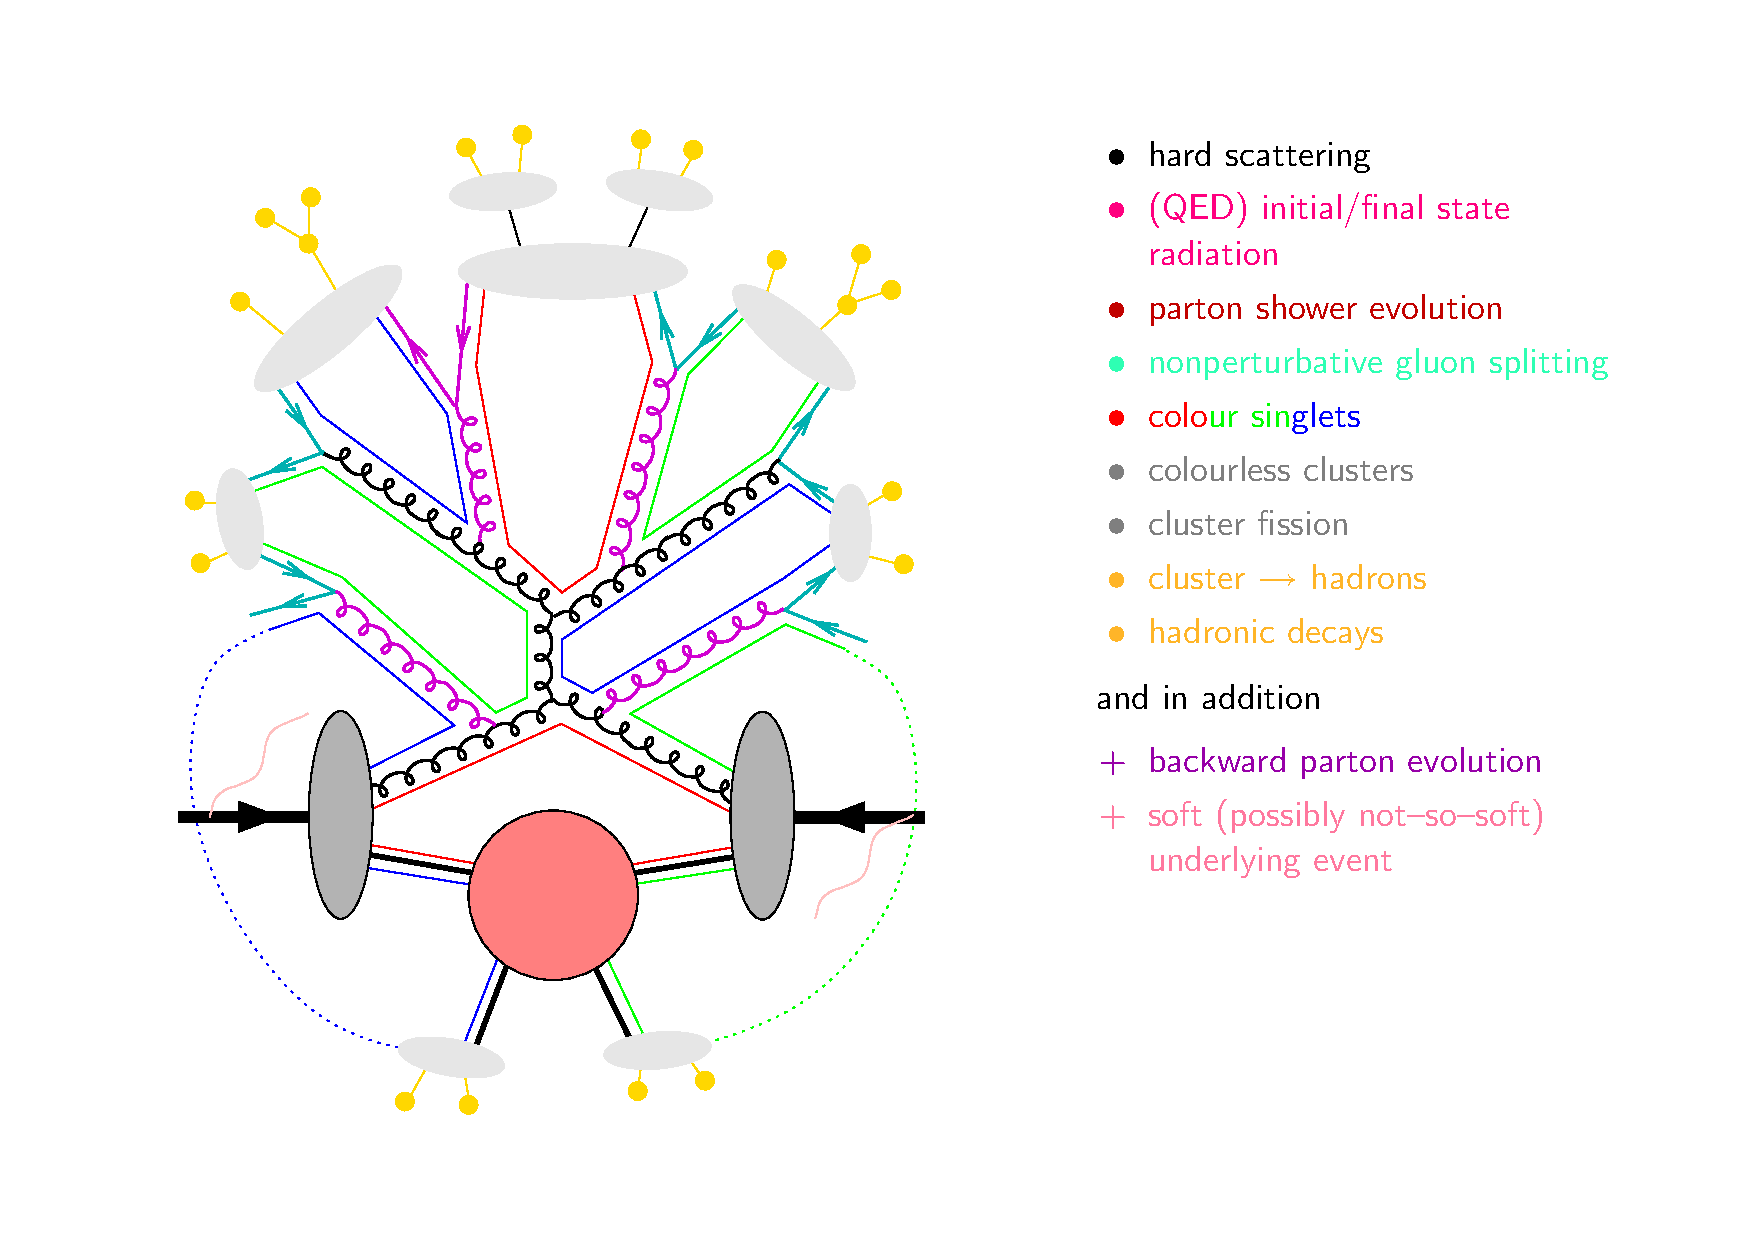
\includegraphics[width=\textwidth]{figures/Zep-soft}
\caption{An illustration of the processes that may surround an interesting event in a proton-proton collision, and the steps required to arrive at a final particle content of that event. In this figure, the dark gray blobs represent the incoming protons and the large red blob represents a hard quark-quark interaction. As illustrated here, the products of such a hard interaction may carry colour charge as well, in which case these products too would need to undergo hadronisation, which, in turn, would show up in the detector as jets. However, since the end product of the process currently under study is photons, which are colourless, that will not be the case here. The upper portion of the figure illustrates the evolution of a secondary gluon interaction, which, though a number of gluon emissions, produces a selection of quark final states that must be gathered into colourless clusters and finally into hadrons. Both stages may undergo further evolution or decay during the process. The final collection of hadrons, which for a single parton interaction will be reasonably well collimated, form a jet of particles in the detector. Similar jet-forming processes may also attach to particles emitted as initial or final state radiation. This figure reproduced from \cite{zep}. For further details on these surrounding processes and their computational representation, see e.g.~\cite{pythman}.
\label{zep}}
\end{figure}

\section{Extended event}
The events produced by the event generator(s) represent the physical process that occurs in the point where two protons interact. Given the limits on our ability to see such interactions, we need to exptend the scope of physical processes in the simulation, to the point where the resulting event information represents something that we might realistically observe with a detector.

The initial and final particle states are fixed in the event generator, however in reality, both initial and final states might easily undergo decay or emission before or after the event occurs, altering the particle content and kinematics of the event. Such initial and final state radiation must be modelled to give an accurate picture of what a detector might see.

Further, final state particles with colour charge will not remain isolated due to colour confinement. These particles will develop a jet of other coloured particles, so that the colour charge becomes obscured to outside observation. The simulation of the process by which colour charged particles combine into colour neutral hadrons is simulated is called hadronisation. Since we are dealing with photons in the final state in the present analysis, this step is not crucial in the events generated to study this process specifically, however $\pi^0$ mesons, one of the major backgrounds to the photon signal, are produced in this way. 

A schematic summary of these processes, along with the steps that the simulation software that models these processes will usually be divided into, is presented in figure~\ref{zep}. In this thesis, the extension of the hard events provided by CalcHEP with these surrounding processes will be carried out in pythia8 \cite{pythia}. Figure~\ref{pythify} illustrates the effect that these surrounding processes have on the distribution of invariant masses.

\begin{figure}[htp]
\centering
\begin{minipage}[b]{.69\textwidth}\hspace{-1.5em}\makebox[0pt][l]{
\noindent\begin{infilsf}
\tiny
\pgfdeclareplotmark{cross} {
\pgfpathmoveto{\pgfpoint{-0.3\pgfplotmarksize}{\pgfplotmarksize}}
\pgfpathlineto{\pgfpoint{+0.3\pgfplotmarksize}{\pgfplotmarksize}}
\pgfpathlineto{\pgfpoint{+0.3\pgfplotmarksize}{0.3\pgfplotmarksize}}
\pgfpathlineto{\pgfpoint{+1\pgfplotmarksize}{0.3\pgfplotmarksize}}
\pgfpathlineto{\pgfpoint{+1\pgfplotmarksize}{-0.3\pgfplotmarksize}}
\pgfpathlineto{\pgfpoint{+0.3\pgfplotmarksize}{-0.3\pgfplotmarksize}}
\pgfpathlineto{\pgfpoint{+0.3\pgfplotmarksize}{-1.\pgfplotmarksize}}
\pgfpathlineto{\pgfpoint{-0.3\pgfplotmarksize}{-1.\pgfplotmarksize}}
\pgfpathlineto{\pgfpoint{-0.3\pgfplotmarksize}{-0.3\pgfplotmarksize}}
\pgfpathlineto{\pgfpoint{-1.\pgfplotmarksize}{-0.3\pgfplotmarksize}}
\pgfpathlineto{\pgfpoint{-1.\pgfplotmarksize}{0.3\pgfplotmarksize}}
\pgfpathlineto{\pgfpoint{-0.3\pgfplotmarksize}{0.3\pgfplotmarksize}}
\pgfpathclose
\pgfusepathqstroke
}
\pgfdeclareplotmark{cross*} {
\pgfpathmoveto{\pgfpoint{-0.3\pgfplotmarksize}{\pgfplotmarksize}}
\pgfpathlineto{\pgfpoint{+0.3\pgfplotmarksize}{\pgfplotmarksize}}
\pgfpathlineto{\pgfpoint{+0.3\pgfplotmarksize}{0.3\pgfplotmarksize}}
\pgfpathlineto{\pgfpoint{+1\pgfplotmarksize}{0.3\pgfplotmarksize}}
\pgfpathlineto{\pgfpoint{+1\pgfplotmarksize}{-0.3\pgfplotmarksize}}
\pgfpathlineto{\pgfpoint{+0.3\pgfplotmarksize}{-0.3\pgfplotmarksize}}
\pgfpathlineto{\pgfpoint{+0.3\pgfplotmarksize}{-1.\pgfplotmarksize}}
\pgfpathlineto{\pgfpoint{-0.3\pgfplotmarksize}{-1.\pgfplotmarksize}}
\pgfpathlineto{\pgfpoint{-0.3\pgfplotmarksize}{-0.3\pgfplotmarksize}}
\pgfpathlineto{\pgfpoint{-1.\pgfplotmarksize}{-0.3\pgfplotmarksize}}
\pgfpathlineto{\pgfpoint{-1.\pgfplotmarksize}{0.3\pgfplotmarksize}}
\pgfpathlineto{\pgfpoint{-0.3\pgfplotmarksize}{0.3\pgfplotmarksize}}
\pgfpathclose
\pgfusepathqfillstroke
}
\pgfdeclareplotmark{newstar} {
\pgfpathmoveto{\pgfqpoint{0pt}{\pgfplotmarksize}}
\pgfpathlineto{\pgfqpointpolar{44}{0.5\pgfplotmarksize}}
\pgfpathlineto{\pgfqpointpolar{18}{\pgfplotmarksize}}
\pgfpathlineto{\pgfqpointpolar{-20}{0.5\pgfplotmarksize}}
\pgfpathlineto{\pgfqpointpolar{-54}{\pgfplotmarksize}}
\pgfpathlineto{\pgfqpointpolar{-90}{0.5\pgfplotmarksize}}
\pgfpathlineto{\pgfqpointpolar{234}{\pgfplotmarksize}}
\pgfpathlineto{\pgfqpointpolar{198}{0.5\pgfplotmarksize}}
\pgfpathlineto{\pgfqpointpolar{162}{\pgfplotmarksize}}
\pgfpathlineto{\pgfqpointpolar{134}{0.5\pgfplotmarksize}}
\pgfpathclose
\pgfusepathqstroke
}
\pgfdeclareplotmark{newstar*} {
\pgfpathmoveto{\pgfqpoint{0pt}{\pgfplotmarksize}}
\pgfpathlineto{\pgfqpointpolar{44}{0.5\pgfplotmarksize}}
\pgfpathlineto{\pgfqpointpolar{18}{\pgfplotmarksize}}
\pgfpathlineto{\pgfqpointpolar{-20}{0.5\pgfplotmarksize}}
\pgfpathlineto{\pgfqpointpolar{-54}{\pgfplotmarksize}}
\pgfpathlineto{\pgfqpointpolar{-90}{0.5\pgfplotmarksize}}
\pgfpathlineto{\pgfqpointpolar{234}{\pgfplotmarksize}}
\pgfpathlineto{\pgfqpointpolar{198}{0.5\pgfplotmarksize}}
\pgfpathlineto{\pgfqpointpolar{162}{\pgfplotmarksize}}
\pgfpathlineto{\pgfqpointpolar{134}{0.5\pgfplotmarksize}}
\pgfpathclose
\pgfusepathqfillstroke
}
\begin{tikzpicture}[x=0.05\textwidth,y=.05\textwidth]

\definecolor{c}{rgb}{0,0,0};
\draw [c] (2,11.8008) -- (2,22.4216) -- (18,22.4216) -- (18,11.8008) -- (2,11.8008);

\definecolor{c}{rgb}{0,0,0};
\draw [c] (2,11.8008) -- (2,22.4216) -- (18,22.4216) -- (18,11.8008) -- (2,11.8008);
\colorlet{c}{kugray!50};
\draw [c] (2.16,22.0847) -- (2.16,22.0869);
\draw [c] (2.16,22.0869) -- (2.16,22.0891);
\draw [c] (2,22.0869) -- (2.16,22.0869);
\draw [c] (2.16,22.0869) -- (2.32,22.0869);
\draw [c] (2.48,20.989) -- (2.48,20.9954);
\draw [c] (2.48,20.9954) -- (2.48,21.0016);
\draw [c] (2.32,20.9954) -- (2.48,20.9954);
\draw [c] (2.48,20.9954) -- (2.64,20.9954);
\draw [c] (2.8,20.2777) -- (2.8,20.2902);
\draw [c] (2.8,20.2902) -- (2.8,20.3024);
\draw [c] (2.64,20.2902) -- (2.8,20.2902);
\draw [c] (2.8,20.2902) -- (2.96,20.2902);
\draw [c] (3.12,19.7357) -- (3.12,19.7568);
\draw [c] (3.12,19.7568) -- (3.12,19.777);
\draw [c] (2.96,19.7568) -- (3.12,19.7568);
\draw [c] (3.12,19.7568) -- (3.28,19.7568);
\draw [c] (3.44,19.2804) -- (3.44,19.313);
\draw [c] (3.44,19.313) -- (3.44,19.3436);
\draw [c] (3.28,19.313) -- (3.44,19.313);
\draw [c] (3.44,19.313) -- (3.6,19.313);
\draw [c] (3.76,18.9425) -- (3.76,18.9876);
\draw [c] (3.76,18.9876) -- (3.76,19.0291);
\draw [c] (3.6,18.9876) -- (3.76,18.9876);
\draw [c] (3.76,18.9876) -- (3.92,18.9876);
\draw [c] (4.08,18.4927) -- (4.08,18.5621);
\draw [c] (4.08,18.5621) -- (4.08,18.6234);
\draw [c] (3.92,18.5621) -- (4.08,18.5621);
\draw [c] (4.08,18.5621) -- (4.24,18.5621);
\draw [c] (4.4,18.1352) -- (4.4,18.2331);
\draw [c] (4.4,18.2331) -- (4.4,18.3154);
\draw [c] (4.24,18.2331) -- (4.4,18.2331);
\draw [c] (4.4,18.2331) -- (4.56,18.2331);
\draw [c] (4.72,17.8253) -- (4.72,17.957);
\draw [c] (4.72,17.957) -- (4.72,18.062);
\draw [c] (4.56,17.957) -- (4.72,17.957);
\draw [c] (4.72,17.957) -- (4.88,17.957);
\draw [c] (5.04,17.7645) -- (5.04,17.8494);
\draw [c] (5.04,17.8494) -- (5.04,17.9225);
\draw [c] (4.88,17.8494) -- (5.04,17.8494);
\draw [c] (5.04,17.8494) -- (5.2,17.8494);
\draw [c] (5.36,17.4837) -- (5.36,17.4878);
\draw [c] (5.36,17.4878) -- (5.36,17.4919);
\draw [c] (5.2,17.4878) -- (5.36,17.4878);
\draw [c] (5.36,17.4878) -- (5.52,17.4878);
\draw [c] (5.68,17.2475) -- (5.68,17.2526);
\draw [c] (5.68,17.2526) -- (5.68,17.2577);
\draw [c] (5.52,17.2526) -- (5.68,17.2526);
\draw [c] (5.68,17.2526) -- (5.84,17.2526);
\draw [c] (6,16.9982) -- (6,17.0047);
\draw [c] (6,17.0047) -- (6,17.0112);
\draw [c] (5.84,17.0047) -- (6,17.0047);
\draw [c] (6,17.0047) -- (6.16,17.0047);
\draw [c] (6.32,16.7792) -- (6.32,16.7873);
\draw [c] (6.32,16.7873) -- (6.32,16.7952);
\draw [c] (6.16,16.7873) -- (6.32,16.7873);
\draw [c] (6.32,16.7873) -- (6.48,16.7873);
\draw [c] (6.64,16.5651) -- (6.64,16.575);
\draw [c] (6.64,16.575) -- (6.64,16.5847);
\draw [c] (6.48,16.575) -- (6.64,16.575);
\draw [c] (6.64,16.575) -- (6.8,16.575);
\draw [c] (6.96,16.3657) -- (6.96,16.3776);
\draw [c] (6.96,16.3776) -- (6.96,16.3893);
\draw [c] (6.8,16.3776) -- (6.96,16.3776);
\draw [c] (6.96,16.3776) -- (7.12,16.3776);
\draw [c] (7.28,16.1641) -- (7.28,16.1786);
\draw [c] (7.28,16.1786) -- (7.28,16.1927);
\draw [c] (7.12,16.1786) -- (7.28,16.1786);
\draw [c] (7.28,16.1786) -- (7.44,16.1786);
\draw [c] (7.6,15.9868) -- (7.6,16.004);
\draw [c] (7.6,16.004) -- (7.6,16.0206);
\draw [c] (7.44,16.004) -- (7.6,16.004);
\draw [c] (7.6,16.004) -- (7.76,16.004);
\draw [c] (7.92,15.7677) -- (7.92,15.7889);
\draw [c] (7.92,15.7889) -- (7.92,15.8093);
\draw [c] (7.76,15.7889) -- (7.92,15.7889);
\draw [c] (7.92,15.7889) -- (8.08,15.7889);
\draw [c] (8.24,15.4855) -- (8.24,15.5133);
\draw [c] (8.24,15.5133) -- (8.24,15.5398);
\draw [c] (8.08,15.5133) -- (8.24,15.5133);
\draw [c] (8.24,15.5133) -- (8.4,15.5133);
\draw [c] (8.56,15.2517) -- (8.56,15.2866);
\draw [c] (8.56,15.2866) -- (8.56,15.3193);
\draw [c] (8.4,15.2866) -- (8.56,15.2866);
\draw [c] (8.56,15.2866) -- (8.72,15.2866);
\draw [c] (8.88,14.9685) -- (8.88,15.0142);
\draw [c] (8.88,15.0142) -- (8.88,15.0563);
\draw [c] (8.72,15.0142) -- (8.88,15.0142);
\draw [c] (8.88,15.0142) -- (9.04,15.0142);
\draw [c] (9.2,14.9072) -- (9.2,14.9557);
\draw [c] (9.2,14.9557) -- (9.2,15.0001);
\draw [c] (9.04,14.9557) -- (9.2,14.9557);
\draw [c] (9.2,14.9557) -- (9.36,14.9557);
\draw [c] (9.52,14.6847) -- (9.52,14.7448);
\draw [c] (9.52,14.7448) -- (9.52,14.7987);
\draw [c] (9.36,14.7448) -- (9.52,14.7448);
\draw [c] (9.52,14.7448) -- (9.68,14.7448);
\draw [c] (9.84,14.3956) -- (9.84,14.4749);
\draw [c] (9.84,14.4749) -- (9.84,14.5437);
\draw [c] (9.68,14.4749) -- (9.84,14.4749);
\draw [c] (9.84,14.4749) -- (10,14.4749);
\draw [c] (10.16,14.24) -- (10.16,14.3321);
\draw [c] (10.16,14.3321) -- (10.16,14.4103);
\draw [c] (10,14.3321) -- (10.16,14.3321);
\draw [c] (10.16,14.3321) -- (10.32,14.3321);
\draw [c] (10.48,13.9492) -- (10.48,14.0709);
\draw [c] (10.48,14.0709) -- (10.48,14.1694);
\draw [c] (10.32,14.0709) -- (10.48,14.0709);
\draw [c] (10.48,14.0709) -- (10.64,14.0709);
\draw [c] (10.8,13.923) -- (10.8,14.0478);
\draw [c] (10.8,14.0478) -- (10.8,14.1483);
\draw [c] (10.64,14.0478) -- (10.8,14.0478);
\draw [c] (10.8,14.0478) -- (10.96,14.0478);
\draw [c] (11.12,13.6051) -- (11.12,13.7741);
\draw [c] (11.12,13.7741) -- (11.12,13.9014);
\draw [c] (10.96,13.7741) -- (11.12,13.7741);
\draw [c] (11.12,13.7741) -- (11.28,13.7741);
\draw [c] (11.44,13.5552) -- (11.44,13.7324);
\draw [c] (11.44,13.7324) -- (11.44,13.8644);
\draw [c] (11.28,13.7324) -- (11.44,13.7324);
\draw [c] (11.44,13.7324) -- (11.6,13.7324);
\draw [c] (11.76,13.5005) -- (11.76,13.6872);
\draw [c] (11.76,13.6872) -- (11.76,13.8243);
\draw [c] (11.6,13.6872) -- (11.76,13.6872);
\draw [c] (11.76,13.6872) -- (11.92,13.6872);
\draw [c] (12.08,12.8003) -- (12.08,13.1609);
\draw [c] (12.08,13.1609) -- (12.08,13.3718);
\draw [c] (11.92,13.1609) -- (12.08,13.1609);
\draw [c] (12.08,13.1609) -- (12.24,13.1609);
\draw [c] (12.4,13.5005) -- (12.4,13.6872);
\draw [c] (12.4,13.6872) -- (12.4,13.8243);
\draw [c] (12.24,13.6872) -- (12.4,13.6872);
\draw [c] (12.4,13.6872) -- (12.56,13.6872);
\draw [c] (12.72,11.8008) -- (12.72,12.4397);
\draw [c] (12.72,12.4397) -- (12.72,12.8003);
\draw [c] (12.56,12.4397) -- (12.72,12.4397);
\draw [c] (12.72,12.4397) -- (12.88,12.4397);
\draw [c] (13.04,11.8008) -- (13.04,12.4397);
\draw [c] (13.04,12.4397) -- (13.04,12.8003);
\draw [c] (12.88,12.4397) -- (13.04,12.4397);
\draw [c] (13.04,12.4397) -- (13.2,12.4397);
\draw [c] (13.36,11.8008) -- (13.36,12.4397);
\draw [c] (13.36,12.4397) -- (13.36,12.8003);
\draw [c] (13.2,12.4397) -- (13.36,12.4397);
\draw [c] (13.36,12.4397) -- (13.52,12.4397);
\draw [c] (13.68,12.1614) -- (13.68,12.8003);
\draw [c] (13.68,12.8003) -- (13.68,13.0785);
\draw [c] (13.52,12.8003) -- (13.68,12.8003);
\draw [c] (13.68,12.8003) -- (13.84,12.8003);
\draw [c] (14,11.8008) -- (14,12.4397);
\draw [c] (14,12.4397) -- (14,12.8003);
\draw [c] (13.84,12.4397) -- (14,12.4397);
\draw [c] (14,12.4397) -- (14.16,12.4397);
\draw [c] (14.32,11.8008) -- (14.32,12.4397);
\draw [c] (14.32,12.4397) -- (14.32,12.8003);
\draw [c] (14.16,12.4397) -- (14.32,12.4397);
\draw [c] (14.32,12.4397) -- (14.48,12.4397);
\draw [c] (14.64,11.8008) -- (14.64,12.4397);
\draw [c] (14.64,12.4397) -- (14.64,12.8003);
\draw [c] (14.48,12.4397) -- (14.64,12.4397);
\draw [c] (14.64,12.4397) -- (14.8,12.4397);
\draw [c] (15.28,11.8008) -- (15.28,12.4397);
\draw [c] (15.28,12.4397) -- (15.28,12.8003);
\draw [c] (15.12,12.4397) -- (15.28,12.4397);
\draw [c] (15.28,12.4397) -- (15.44,12.4397);
\definecolor{c}{rgb}{0,0,0};
\draw [c] (2,11.8008) -- (18,11.8008);
\draw [c] (3.30612,12.084) -- (3.30612,11.8008);
\draw [c] (3.63265,11.9424) -- (3.63265,11.8008);
\draw [c] (3.95918,11.9424) -- (3.95918,11.8008);
\draw [c] (4.28571,11.9424) -- (4.28571,11.8008);
\draw [c] (4.61225,11.9424) -- (4.61225,11.8008);
\draw [c] (4.93878,12.084) -- (4.93878,11.8008);
\draw [c] (5.26531,11.9424) -- (5.26531,11.8008);
\draw [c] (5.59184,11.9424) -- (5.59184,11.8008);
\draw [c] (5.91837,11.9424) -- (5.91837,11.8008);
\draw [c] (6.2449,11.9424) -- (6.2449,11.8008);
\draw [c] (6.57143,12.084) -- (6.57143,11.8008);
\draw [c] (6.89796,11.9424) -- (6.89796,11.8008);
\draw [c] (7.22449,11.9424) -- (7.22449,11.8008);
\draw [c] (7.55102,11.9424) -- (7.55102,11.8008);
\draw [c] (7.87755,11.9424) -- (7.87755,11.8008);
\draw [c] (8.20408,12.084) -- (8.20408,11.8008);
\draw [c] (8.53061,11.9424) -- (8.53061,11.8008);
\draw [c] (8.85714,11.9424) -- (8.85714,11.8008);
\draw [c] (9.18367,11.9424) -- (9.18367,11.8008);
\draw [c] (9.5102,11.9424) -- (9.5102,11.8008);
\draw [c] (9.83673,12.084) -- (9.83673,11.8008);
\draw [c] (10.1633,11.9424) -- (10.1633,11.8008);
\draw [c] (10.4898,11.9424) -- (10.4898,11.8008);
\draw [c] (10.8163,11.9424) -- (10.8163,11.8008);
\draw [c] (11.1429,11.9424) -- (11.1429,11.8008);
\draw [c] (11.4694,12.084) -- (11.4694,11.8008);
\draw [c] (11.7959,11.9424) -- (11.7959,11.8008);
\draw [c] (12.1224,11.9424) -- (12.1224,11.8008);
\draw [c] (12.449,11.9424) -- (12.449,11.8008);
\draw [c] (12.7755,11.9424) -- (12.7755,11.8008);
\draw [c] (13.102,12.084) -- (13.102,11.8008);
\draw [c] (13.4286,11.9424) -- (13.4286,11.8008);
\draw [c] (13.7551,11.9424) -- (13.7551,11.8008);
\draw [c] (14.0816,11.9424) -- (14.0816,11.8008);
\draw [c] (14.4082,11.9424) -- (14.4082,11.8008);
\draw [c] (14.7347,12.084) -- (14.7347,11.8008);
\draw [c] (15.0612,11.9424) -- (15.0612,11.8008);
\draw [c] (15.3878,11.9424) -- (15.3878,11.8008);
\draw [c] (15.7143,11.9424) -- (15.7143,11.8008);
\draw [c] (16.0408,11.9424) -- (16.0408,11.8008);
\draw [c] (16.3673,12.084) -- (16.3673,11.8008);
\draw [c] (16.6939,11.9424) -- (16.6939,11.8008);
\draw [c] (17.0204,11.9424) -- (17.0204,11.8008);
\draw [c] (17.3469,11.9424) -- (17.3469,11.8008);
\draw [c] (17.6735,11.9424) -- (17.6735,11.8008);
\draw [c] (18,12.084) -- (18,11.8008);
\draw [c] (3.30612,12.084) -- (3.30612,11.8008);
\draw [c] (2.97959,11.9424) -- (2.97959,11.8008);
\draw [c] (2.65306,11.9424) -- (2.65306,11.8008);
\draw [c] (2.32653,11.9424) -- (2.32653,11.8008);

\draw [c] (2,11.8008) -- (2,22.4216);
\draw [anchor= east] (0.1,22.4216) node[ rotate=90]{$\di\sigma/\di M_{\gamma\gamma}$ [pb/GeV]};
\draw [c] (2.27,11.8185) -- (2,11.8185);
\draw [c] (2.27,11.8986) -- (2,11.8986);
\draw [c] (2.27,11.9681) -- (2,11.9681);
\draw [c] (2.27,12.0294) -- (2,12.0294);
\draw [c] (2.54,12.0842) -- (2,12.0842);
\draw [anchor= east] (1.844,12.0842) node[ rotate=0]{$10^{-10}$};
\draw [c] (2.27,12.4448) -- (2,12.4448);
\draw [c] (2.27,12.6558) -- (2,12.6558);
\draw [c] (2.27,12.8054) -- (2,12.8054);
\draw [c] (2.27,12.9215) -- (2,12.9215);
\draw [c] (2.27,13.0164) -- (2,13.0164);
\draw [c] (2.27,13.0966) -- (2,13.0966);
\draw [c] (2.27,13.166) -- (2,13.166);
\draw [c] (2.27,13.2273) -- (2,13.2273);
\draw [c] (2.54,13.2821) -- (2,13.2821);
\draw [anchor= east] (1.844,13.2821) node[ rotate=0]{$10^{-9}$};
\draw [c] (2.27,13.6427) -- (2,13.6427);
\draw [c] (2.27,13.8537) -- (2,13.8537);
\draw [c] (2.27,14.0033) -- (2,14.0033);
\draw [c] (2.27,14.1194) -- (2,14.1194);
\draw [c] (2.27,14.2143) -- (2,14.2143);
\draw [c] (2.27,14.2945) -- (2,14.2945);
\draw [c] (2.27,14.364) -- (2,14.364);
\draw [c] (2.27,14.4252) -- (2,14.4252);
\draw [c] (2.54,14.48) -- (2,14.48);
\draw [anchor= east] (1.844,14.48) node[ rotate=0]{$10^{-8}$};
\draw [c] (2.27,14.8407) -- (2,14.8407);
\draw [c] (2.27,15.0516) -- (2,15.0516);
\draw [c] (2.27,15.2013) -- (2,15.2013);
\draw [c] (2.27,15.3174) -- (2,15.3174);
\draw [c] (2.27,15.4122) -- (2,15.4122);
\draw [c] (2.27,15.4924) -- (2,15.4924);
\draw [c] (2.27,15.5619) -- (2,15.5619);
\draw [c] (2.27,15.6231) -- (2,15.6231);
\draw [c] (2.54,15.678) -- (2,15.678);
\draw [anchor= east] (1.844,15.678) node[ rotate=0]{$10^{-7}$};
\draw [c] (2.27,16.0386) -- (2,16.0386);
\draw [c] (2.27,16.2495) -- (2,16.2495);
\draw [c] (2.27,16.3992) -- (2,16.3992);
\draw [c] (2.27,16.5153) -- (2,16.5153);
\draw [c] (2.27,16.6101) -- (2,16.6101);
\draw [c] (2.27,16.6903) -- (2,16.6903);
\draw [c] (2.27,16.7598) -- (2,16.7598);
\draw [c] (2.27,16.8211) -- (2,16.8211);
\draw [c] (2.54,16.8759) -- (2,16.8759);
\draw [anchor= east] (1.844,16.8759) node[ rotate=0]{$10^{-6}$};
\draw [c] (2.27,17.2365) -- (2,17.2365);
\draw [c] (2.27,17.4474) -- (2,17.4474);
\draw [c] (2.27,17.5971) -- (2,17.5971);
\draw [c] (2.27,17.7132) -- (2,17.7132);
\draw [c] (2.27,17.808) -- (2,17.808);
\draw [c] (2.27,17.8882) -- (2,17.8882);
\draw [c] (2.27,17.9577) -- (2,17.9577);
\draw [c] (2.27,18.019) -- (2,18.019);
\draw [c] (2.54,18.0738) -- (2,18.0738);
\draw [anchor= east] (1.844,18.0738) node[ rotate=0]{$10^{-5}$};
\draw [c] (2.27,18.4344) -- (2,18.4344);
\draw [c] (2.27,18.6453) -- (2,18.6453);
\draw [c] (2.27,18.795) -- (2,18.795);
\draw [c] (2.27,18.9111) -- (2,18.9111);
\draw [c] (2.27,19.006) -- (2,19.006);
\draw [c] (2.27,19.0861) -- (2,19.0861);
\draw [c] (2.27,19.1556) -- (2,19.1556);
\draw [c] (2.27,19.2169) -- (2,19.2169);
\draw [c] (2.54,19.2717) -- (2,19.2717);
\draw [anchor= east] (1.844,19.2717) node[ rotate=0]{$10^{-4}$};
\draw [c] (2.27,19.6323) -- (2,19.6323);
\draw [c] (2.27,19.8433) -- (2,19.8433);
\draw [c] (2.27,19.9929) -- (2,19.9929);
\draw [c] (2.27,20.109) -- (2,20.109);
\draw [c] (2.27,20.2039) -- (2,20.2039);
\draw [c] (2.27,20.2841) -- (2,20.2841);
\draw [c] (2.27,20.3535) -- (2,20.3535);
\draw [c] (2.27,20.4148) -- (2,20.4148);
\draw [c] (2.54,20.4696) -- (2,20.4696);
\draw [anchor= east] (1.844,20.4696) node[ rotate=0]{$10^{-3}$};
\draw [c] (2.27,20.8302) -- (2,20.8302);
\draw [c] (2.27,21.0412) -- (2,21.0412);
\draw [c] (2.27,21.1908) -- (2,21.1908);
\draw [c] (2.27,21.3069) -- (2,21.3069);
\draw [c] (2.27,21.4018) -- (2,21.4018);
\draw [c] (2.27,21.482) -- (2,21.482);
\draw [c] (2.27,21.5515) -- (2,21.5515);
\draw [c] (2.27,21.6127) -- (2,21.6127);
\draw [c] (2.54,21.6675) -- (2,21.6675);
\draw [anchor= east] (1.844,21.6675) node[ rotate=0]{$10^{-2}$};
\draw [c] (2.27,22.0282) -- (2,22.0282);
\draw [c] (2.27,22.2391) -- (2,22.2391);
\draw [c] (2.27,22.3888) -- (2,22.3888);
\colorlet{c}{kugray};
\draw [c] (2.16,21.9886) -- (2.16,21.9911);
\draw [c] (2.16,21.9911) -- (2.16,21.9935);
\draw [c] (2,21.9911) -- (2.16,21.9911);
\draw [c] (2.16,21.9911) -- (2.32,21.9911);
\draw [c] (2.48,20.8999) -- (2.48,20.9067);
\draw [c] (2.48,20.9067) -- (2.48,20.9135);
\draw [c] (2.32,20.9067) -- (2.48,20.9067);
\draw [c] (2.48,20.9067) -- (2.64,20.9067);
\draw [c] (2.8,20.1651) -- (2.8,20.179);
\draw [c] (2.8,20.179) -- (2.8,20.1926);
\draw [c] (2.64,20.179) -- (2.8,20.179);
\draw [c] (2.8,20.179) -- (2.96,20.179);
\draw [c] (3.12,19.6256) -- (3.12,19.649);
\draw [c] (3.12,19.649) -- (3.12,19.6714);
\draw [c] (2.96,19.649) -- (3.12,19.649);
\draw [c] (3.12,19.649) -- (3.28,19.649);
\draw [c] (3.44,19.2037) -- (3.44,19.2388);
\draw [c] (3.44,19.2388) -- (3.44,19.2717);
\draw [c] (3.28,19.2388) -- (3.44,19.2388);
\draw [c] (3.44,19.2388) -- (3.6,19.2388);
\draw [c] (3.76,18.8394) -- (3.76,18.8892);
\draw [c] (3.76,18.8892) -- (3.76,18.9346);
\draw [c] (3.6,18.8892) -- (3.76,18.8892);
\draw [c] (3.76,18.8892) -- (3.92,18.8892);
\draw [c] (4.08,18.3977) -- (4.08,18.4738);
\draw [c] (4.08,18.4738) -- (4.08,18.5401);
\draw [c] (3.92,18.4738) -- (4.08,18.4738);
\draw [c] (4.08,18.4738) -- (4.24,18.4738);
\draw [c] (4.4,18.0231) -- (4.4,18.1321);
\draw [c] (4.4,18.1321) -- (4.4,18.2221);
\draw [c] (4.24,18.1321) -- (4.4,18.1321);
\draw [c] (4.4,18.1321) -- (4.56,18.1321);
\draw [c] (4.72,17.5639) -- (4.72,17.7329);
\draw [c] (4.72,17.7329) -- (4.72,17.8603);
\draw [c] (4.56,17.7329) -- (4.72,17.7329);
\draw [c] (4.72,17.7329) -- (4.88,17.7329);
\draw [c] (5.04,17.6487) -- (5.04,17.7446);
\draw [c] (5.04,17.7446) -- (5.04,17.8255);
\draw [c] (4.88,17.7446) -- (5.04,17.7446);
\draw [c] (5.04,17.7446) -- (5.2,17.7446);
\draw [c] (5.36,17.3748) -- (5.36,17.3793);
\draw [c] (5.36,17.3793) -- (5.36,17.3838);
\draw [c] (5.2,17.3793) -- (5.36,17.3793);
\draw [c] (5.36,17.3793) -- (5.52,17.3793);
\draw [c] (5.68,17.1419) -- (5.68,17.1476);
\draw [c] (5.68,17.1476) -- (5.68,17.1532);
\draw [c] (5.52,17.1476) -- (5.68,17.1476);
\draw [c] (5.68,17.1476) -- (5.84,17.1476);
\draw [c] (6,16.8903) -- (6,16.8975);
\draw [c] (6,16.8975) -- (6,16.9046);
\draw [c] (5.84,16.8975) -- (6,16.8975);
\draw [c] (6,16.8975) -- (6.16,16.8975);
\draw [c] (6.32,16.6718) -- (6.32,16.6807);
\draw [c] (6.32,16.6807) -- (6.32,16.6894);
\draw [c] (6.16,16.6807) -- (6.32,16.6807);
\draw [c] (6.32,16.6807) -- (6.48,16.6807);
\draw [c] (6.64,16.4482) -- (6.64,16.4592);
\draw [c] (6.64,16.4592) -- (6.64,16.47);
\draw [c] (6.48,16.4592) -- (6.64,16.4592);
\draw [c] (6.64,16.4592) -- (6.8,16.4592);
\draw [c] (6.96,16.2518) -- (6.96,16.2651);
\draw [c] (6.96,16.2651) -- (6.96,16.2781);
\draw [c] (6.8,16.2651) -- (6.96,16.2651);
\draw [c] (6.96,16.2651) -- (7.12,16.2651);
\draw [c] (7.28,16.043) -- (7.28,16.0593);
\draw [c] (7.28,16.0593) -- (7.28,16.0751);
\draw [c] (7.12,16.0593) -- (7.28,16.0593);
\draw [c] (7.28,16.0593) -- (7.44,16.0593);
\draw [c] (7.6,15.8872) -- (7.6,15.9061);
\draw [c] (7.6,15.9061) -- (7.6,15.9244);
\draw [c] (7.44,15.9061) -- (7.6,15.9061);
\draw [c] (7.6,15.9061) -- (7.76,15.9061);
\draw [c] (7.92,15.6564) -- (7.92,15.68);
\draw [c] (7.92,15.68) -- (7.92,15.7026);
\draw [c] (7.76,15.68) -- (7.92,15.68);
\draw [c] (7.92,15.68) -- (8.08,15.68);
\draw [c] (8.24,15.3725) -- (8.24,15.4036);
\draw [c] (8.24,15.4036) -- (8.24,15.4329);
\draw [c] (8.08,15.4036) -- (8.24,15.4036);
\draw [c] (8.24,15.4036) -- (8.4,15.4036);
\draw [c] (8.56,15.1099) -- (8.56,15.1499);
\draw [c] (8.56,15.1499) -- (8.56,15.187);
\draw [c] (8.4,15.1499) -- (8.56,15.1499);
\draw [c] (8.56,15.1499) -- (8.72,15.1499);
\draw [c] (8.88,14.862) -- (8.88,14.9127);
\draw [c] (8.88,14.9127) -- (8.88,14.9589);
\draw [c] (8.72,14.9127) -- (8.88,14.9127);
\draw [c] (8.88,14.9127) -- (9.04,14.9127);
\draw [c] (9.2,14.8126) -- (9.2,14.8658);
\draw [c] (9.2,14.8658) -- (9.2,14.914);
\draw [c] (9.04,14.8658) -- (9.2,14.8658);
\draw [c] (9.2,14.8658) -- (9.36,14.8658);
\draw [c] (9.52,14.5837) -- (9.52,14.6499);
\draw [c] (9.52,14.6499) -- (9.52,14.7087);
\draw [c] (9.36,14.6499) -- (9.52,14.6499);
\draw [c] (9.52,14.6499) -- (9.68,14.6499);
\draw [c] (9.84,14.2548) -- (9.84,14.3456);
\draw [c] (9.84,14.3456) -- (9.84,14.4229);
\draw [c] (9.68,14.3456) -- (9.84,14.3456);
\draw [c] (9.84,14.3456) -- (10,14.3456);
\draw [c] (10.16,14.1042) -- (10.16,14.2091);
\draw [c] (10.16,14.2091) -- (10.16,14.2964);
\draw [c] (10,14.2091) -- (10.16,14.2091);
\draw [c] (10.16,14.2091) -- (10.32,14.2091);
\draw [c] (10.48,13.7691) -- (10.48,13.9136);
\draw [c] (10.48,13.9136) -- (10.48,14.0266);
\draw [c] (10.32,13.9136) -- (10.48,13.9136);
\draw [c] (10.48,13.9136) -- (10.64,13.9136);
\draw [c] (10.8,13.7691) -- (10.8,13.9136);
\draw [c] (10.8,13.9136) -- (10.8,14.0266);
\draw [c] (10.64,13.9136) -- (10.8,13.9136);
\draw [c] (10.8,13.9136) -- (10.96,13.9136);
\draw [c] (11.12,13.5005) -- (11.12,13.6872);
\draw [c] (11.12,13.6872) -- (11.12,13.8243);
\draw [c] (10.96,13.6872) -- (11.12,13.6872);
\draw [c] (11.12,13.6872) -- (11.28,13.6872);
\draw [c] (11.44,13.4398) -- (11.44,13.6376);
\draw [c] (11.44,13.6376) -- (11.44,13.7805);
\draw [c] (11.28,13.6376) -- (11.44,13.6376);
\draw [c] (11.44,13.6376) -- (11.6,13.6376);
\draw [c] (11.76,13.3718) -- (11.76,13.5828);
\draw [c] (11.76,13.5828) -- (11.76,13.7324);
\draw [c] (11.6,13.5828) -- (11.76,13.5828);
\draw [c] (11.76,13.5828) -- (11.92,13.5828);
\draw [c] (12.08,12.1614) -- (12.08,12.8003);
\draw [c] (12.08,12.8003) -- (12.08,13.0785);
\draw [c] (11.92,12.8003) -- (12.08,12.8003);
\draw [c] (12.08,12.8003) -- (12.24,12.8003);
\draw [c] (12.4,13.4398) -- (12.4,13.6376);
\draw [c] (12.4,13.6376) -- (12.4,13.7805);
\draw [c] (12.24,13.6376) -- (12.4,13.6376);
\draw [c] (12.4,13.6376) -- (12.56,13.6376);
\draw [c] (13.04,11.8008) -- (13.04,12.4397);
\draw [c] (13.04,12.4397) -- (13.04,12.8003);
\draw [c] (12.88,12.4397) -- (13.04,12.4397);
\draw [c] (13.04,12.4397) -- (13.2,12.4397);
\draw [c] (13.36,11.8008) -- (13.36,12.4397);
\draw [c] (13.36,12.4397) -- (13.36,12.8003);
\draw [c] (13.2,12.4397) -- (13.36,12.4397);
\draw [c] (13.36,12.4397) -- (13.52,12.4397);
\draw [c] (13.68,11.8008) -- (13.68,12.4397);
\draw [c] (13.68,12.4397) -- (13.68,12.8003);
\draw [c] (13.52,12.4397) -- (13.68,12.4397);
\draw [c] (13.68,12.4397) -- (13.84,12.4397);
\colorlet{c}{natgreen!50};
\draw [c] (2.16,22.0854) -- (2.16,22.0876);
\draw [c] (2.16,22.0876) -- (2.16,22.0898);
\draw [c] (2,22.0876) -- (2.16,22.0876);
\draw [c] (2.16,22.0876) -- (2.32,22.0876);
\draw [c] (2.48,21.0058) -- (2.48,21.012);
\draw [c] (2.48,21.012) -- (2.48,21.0181);
\draw [c] (2.32,21.012) -- (2.48,21.012);
\draw [c] (2.48,21.012) -- (2.64,21.012);
\draw [c] (2.8,20.2599) -- (2.8,20.2726);
\draw [c] (2.8,20.2726) -- (2.8,20.2851);
\draw [c] (2.64,20.2726) -- (2.8,20.2726);
\draw [c] (2.8,20.2726) -- (2.96,20.2726);
\draw [c] (3.12,19.7099) -- (3.12,19.7315);
\draw [c] (3.12,19.7315) -- (3.12,19.7522);
\draw [c] (2.96,19.7315) -- (3.12,19.7315);
\draw [c] (3.12,19.7315) -- (3.28,19.7315);
\draw [c] (3.44,19.3211) -- (3.44,19.3525);
\draw [c] (3.44,19.3525) -- (3.44,19.3821);
\draw [c] (3.28,19.3525) -- (3.44,19.3525);
\draw [c] (3.44,19.3525) -- (3.6,19.3525);
\draw [c] (3.76,18.928) -- (3.76,18.9738);
\draw [c] (3.76,18.9738) -- (3.76,19.0158);
\draw [c] (3.6,18.9738) -- (3.76,18.9738);
\draw [c] (3.76,18.9738) -- (3.92,18.9738);
\draw [c] (4.08,18.5665) -- (4.08,18.6313);
\draw [c] (4.08,18.6313) -- (4.08,18.6889);
\draw [c] (3.92,18.6313) -- (4.08,18.6313);
\draw [c] (4.08,18.6313) -- (4.24,18.6313);
\draw [c] (4.4,18.2956) -- (4.4,18.3796);
\draw [c] (4.4,18.3796) -- (4.4,18.4519);
\draw [c] (4.24,18.3796) -- (4.4,18.3796);
\draw [c] (4.4,18.3796) -- (4.56,18.3796);
\draw [c] (4.72,18.0441) -- (4.72,18.151);
\draw [c] (4.72,18.151) -- (4.72,18.2396);
\draw [c] (4.56,18.151) -- (4.72,18.151);
\draw [c] (4.72,18.151) -- (4.88,18.151);
\draw [c] (5.04,17.8055) -- (5.04,17.8627);
\draw [c] (5.04,17.8627) -- (5.04,17.9143);
\draw [c] (4.88,17.8627) -- (5.04,17.8627);
\draw [c] (5.04,17.8627) -- (5.2,17.8627);
\draw [c] (5.36,17.6929) -- (5.36,17.6978);
\draw [c] (5.36,17.6978) -- (5.36,17.7026);
\draw [c] (5.2,17.6978) -- (5.36,17.6978);
\draw [c] (5.36,17.6978) -- (5.52,17.6978);
\draw [c] (5.68,17.5229) -- (5.68,17.5286);
\draw [c] (5.68,17.5286) -- (5.68,17.5343);
\draw [c] (5.52,17.5286) -- (5.68,17.5286);
\draw [c] (5.68,17.5286) -- (5.84,17.5286);
\draw [c] (6,17.3746) -- (6,17.3812);
\draw [c] (6,17.3812) -- (6,17.3877);
\draw [c] (5.84,17.3812) -- (6,17.3812);
\draw [c] (6,17.3812) -- (6.16,17.3812);
\draw [c] (6.32,17.2692) -- (6.32,17.2765);
\draw [c] (6.32,17.2765) -- (6.32,17.2837);
\draw [c] (6.16,17.2765) -- (6.32,17.2765);
\draw [c] (6.32,17.2765) -- (6.48,17.2765);
\draw [c] (6.64,17.1541) -- (6.64,17.1623);
\draw [c] (6.64,17.1623) -- (6.64,17.1703);
\draw [c] (6.48,17.1623) -- (6.64,17.1623);
\draw [c] (6.64,17.1623) -- (6.8,17.1623);
\draw [c] (6.96,17.0606) -- (6.96,17.0695);
\draw [c] (6.96,17.0695) -- (6.96,17.0783);
\draw [c] (6.8,17.0695) -- (6.96,17.0695);
\draw [c] (6.96,17.0695) -- (7.12,17.0695);
\draw [c] (7.28,16.9827) -- (7.28,16.9923);
\draw [c] (7.28,16.9923) -- (7.28,17.0018);
\draw [c] (7.12,16.9923) -- (7.28,16.9923);
\draw [c] (7.28,16.9923) -- (7.44,16.9923);
\draw [c] (7.6,16.9271) -- (7.6,16.9372);
\draw [c] (7.6,16.9372) -- (7.6,16.9472);
\draw [c] (7.44,16.9372) -- (7.6,16.9372);
\draw [c] (7.6,16.9372) -- (7.76,16.9372);
\draw [c] (7.92,16.8537) -- (7.92,16.8646);
\draw [c] (7.92,16.8646) -- (7.92,16.8752);
\draw [c] (7.76,16.8646) -- (7.92,16.8646);
\draw [c] (7.92,16.8646) -- (8.08,16.8646);
\draw [c] (8.24,16.8089) -- (8.24,16.8203);
\draw [c] (8.24,16.8203) -- (8.24,16.8314);
\draw [c] (8.08,16.8203) -- (8.24,16.8203);
\draw [c] (8.24,16.8203) -- (8.4,16.8203);
\draw [c] (8.56,16.7645) -- (8.56,16.7764);
\draw [c] (8.56,16.7764) -- (8.56,16.788);
\draw [c] (8.4,16.7764) -- (8.56,16.7764);
\draw [c] (8.56,16.7764) -- (8.72,16.7764);
\draw [c] (8.88,16.7259) -- (8.88,16.7382);
\draw [c] (8.88,16.7382) -- (8.88,16.7502);
\draw [c] (8.72,16.7382) -- (8.88,16.7382);
\draw [c] (8.88,16.7382) -- (9.04,16.7382);
\draw [c] (9.2,16.6876) -- (9.2,16.7004);
\draw [c] (9.2,16.7004) -- (9.2,16.7129);
\draw [c] (9.04,16.7004) -- (9.2,16.7004);
\draw [c] (9.2,16.7004) -- (9.36,16.7004);
\draw [c] (9.52,16.6177) -- (9.52,16.6314);
\draw [c] (9.52,16.6314) -- (9.52,16.6447);
\draw [c] (9.36,16.6314) -- (9.52,16.6314);
\draw [c] (9.52,16.6314) -- (9.68,16.6314);
\draw [c] (9.84,16.5889) -- (9.84,16.603);
\draw [c] (9.84,16.603) -- (9.84,16.6167);
\draw [c] (9.68,16.603) -- (9.84,16.603);
\draw [c] (9.84,16.603) -- (10,16.603);
\draw [c] (10.16,16.5341) -- (10.16,16.5489);
\draw [c] (10.16,16.5489) -- (10.16,16.5633);
\draw [c] (10,16.5489) -- (10.16,16.5489);
\draw [c] (10.16,16.5489) -- (10.32,16.5489);
\draw [c] (10.48,16.4921) -- (10.48,16.5075);
\draw [c] (10.48,16.5075) -- (10.48,16.5225);
\draw [c] (10.32,16.5075) -- (10.48,16.5075);
\draw [c] (10.48,16.5075) -- (10.64,16.5075);
\draw [c] (10.8,16.4375) -- (10.8,16.4538);
\draw [c] (10.8,16.4538) -- (10.8,16.4696);
\draw [c] (10.64,16.4538) -- (10.8,16.4538);
\draw [c] (10.8,16.4538) -- (10.96,16.4538);
\draw [c] (11.12,16.3965) -- (11.12,16.4134);
\draw [c] (11.12,16.4134) -- (11.12,16.4298);
\draw [c] (10.96,16.4134) -- (11.12,16.4134);
\draw [c] (11.12,16.4134) -- (11.28,16.4134);
\draw [c] (11.44,16.3364) -- (11.44,16.3543);
\draw [c] (11.44,16.3543) -- (11.44,16.3716);
\draw [c] (11.28,16.3543) -- (11.44,16.3543);
\draw [c] (11.44,16.3543) -- (11.6,16.3543);
\draw [c] (11.76,16.263) -- (11.76,16.2822);
\draw [c] (11.76,16.2822) -- (11.76,16.3007);
\draw [c] (11.6,16.2822) -- (11.76,16.2822);
\draw [c] (11.76,16.2822) -- (11.92,16.2822);
\draw [c] (12.08,16.2328) -- (12.08,16.2526);
\draw [c] (12.08,16.2526) -- (12.08,16.2717);
\draw [c] (11.92,16.2526) -- (12.08,16.2526);
\draw [c] (12.08,16.2526) -- (12.24,16.2526);
\draw [c] (12.4,16.1643) -- (12.4,16.1854);
\draw [c] (12.4,16.1854) -- (12.4,16.2057);
\draw [c] (12.24,16.1854) -- (12.4,16.1854);
\draw [c] (12.4,16.1854) -- (12.56,16.1854);
\draw [c] (12.72,16.1018) -- (12.72,16.1242);
\draw [c] (12.72,16.1242) -- (12.72,16.1457);
\draw [c] (12.56,16.1242) -- (12.72,16.1242);
\draw [c] (12.72,16.1242) -- (12.88,16.1242);
\draw [c] (13.04,15.9736) -- (13.04,15.999);
\draw [c] (13.04,15.999) -- (13.04,16.0232);
\draw [c] (12.88,15.999) -- (13.04,15.999);
\draw [c] (13.04,15.999) -- (13.2,15.999);
\draw [c] (13.36,15.9321) -- (13.36,15.9586);
\draw [c] (13.36,15.9586) -- (13.36,15.9837);
\draw [c] (13.2,15.9586) -- (13.36,15.9586);
\draw [c] (13.36,15.9586) -- (13.52,15.9586);
\draw [c] (13.68,15.7989) -- (13.68,15.8289);
\draw [c] (13.68,15.8289) -- (13.68,15.8573);
\draw [c] (13.52,15.8289) -- (13.68,15.8289);
\draw [c] (13.68,15.8289) -- (13.84,15.8289);
\draw [c] (14,15.7439) -- (14,15.7755);
\draw [c] (14,15.7755) -- (14,15.8054);
\draw [c] (13.84,15.7755) -- (14,15.7755);
\draw [c] (14,15.7755) -- (14.16,15.7755);
\draw [c] (14.32,15.6009) -- (14.32,15.6372);
\draw [c] (14.32,15.6372) -- (14.32,15.6712);
\draw [c] (14.16,15.6372) -- (14.32,15.6372);
\draw [c] (14.32,15.6372) -- (14.48,15.6372);
\draw [c] (14.64,15.4985) -- (14.64,15.5386);
\draw [c] (14.64,15.5386) -- (14.64,15.5758);
\draw [c] (14.48,15.5386) -- (14.64,15.5386);
\draw [c] (14.64,15.5386) -- (14.8,15.5386);
\draw [c] (14.96,15.4253) -- (14.96,15.4683);
\draw [c] (14.96,15.4683) -- (14.96,15.508);
\draw [c] (14.8,15.4683) -- (14.96,15.4683);
\draw [c] (14.96,15.4683) -- (15.12,15.4683);
\draw [c] (15.28,15.3282) -- (15.28,15.3754);
\draw [c] (15.28,15.3754) -- (15.28,15.4187);
\draw [c] (15.12,15.3754) -- (15.28,15.3754);
\draw [c] (15.28,15.3754) -- (15.44,15.3754);
\draw [c] (15.6,15.199) -- (15.6,15.2524);
\draw [c] (15.6,15.2524) -- (15.6,15.3009);
\draw [c] (15.44,15.2524) -- (15.6,15.2524);
\draw [c] (15.6,15.2524) -- (15.76,15.2524);
\draw [c] (15.92,15.2042) -- (15.92,15.2574);
\draw [c] (15.92,15.2574) -- (15.92,15.3056);
\draw [c] (15.76,15.2574) -- (15.92,15.2574);
\draw [c] (15.92,15.2574) -- (16.08,15.2574);
\draw [c] (16.24,14.8508) -- (16.24,14.9254);
\draw [c] (16.24,14.9254) -- (16.24,14.9906);
\draw [c] (16.08,14.9254) -- (16.24,14.9254);
\draw [c] (16.24,14.9254) -- (16.4,14.9254);
\draw [c] (16.56,14.7149) -- (16.56,14.7999);
\draw [c] (16.56,14.7999) -- (16.56,14.873);
\draw [c] (16.4,14.7999) -- (16.56,14.7999);
\draw [c] (16.56,14.7999) -- (16.72,14.7999);
\draw [c] (16.88,14.6163) -- (16.88,14.7098);
\draw [c] (16.88,14.7098) -- (16.88,14.789);
\draw [c] (16.72,14.7098) -- (16.88,14.7098);
\draw [c] (16.88,14.7098) -- (17.04,14.7098);
\draw [c] (17.2,14.4347) -- (17.2,14.5459);
\draw [c] (17.2,14.5459) -- (17.2,14.6374);
\draw [c] (17.04,14.5459) -- (17.2,14.5459);
\draw [c] (17.2,14.5459) -- (17.36,14.5459);
\draw [c] (17.52,14.124) -- (17.52,14.2736);
\draw [c] (17.52,14.2736) -- (17.52,14.3897);
\draw [c] (17.36,14.2736) -- (17.52,14.2736);
\draw [c] (17.52,14.2736) -- (17.68,14.2736);
\draw [c] (17.84,13.8314) -- (17.84,14.0291);
\draw [c] (17.84,14.0291) -- (17.84,14.1721);
\draw [c] (17.68,14.0291) -- (17.84,14.0291);
\draw [c] (17.84,14.0291) -- (18,14.0291);
\colorlet{c}{natgreen};
\draw [c] (2.16,21.9864) -- (2.16,21.9888);
\draw [c] (2.16,21.9888) -- (2.16,21.9913);
\draw [c] (2,21.9888) -- (2.16,21.9888);
\draw [c] (2.16,21.9888) -- (2.32,21.9888);
\draw [c] (2.48,20.9164) -- (2.48,20.9232);
\draw [c] (2.48,20.9232) -- (2.48,20.9299);
\draw [c] (2.32,20.9232) -- (2.48,20.9232);
\draw [c] (2.48,20.9232) -- (2.64,20.9232);
\draw [c] (2.8,20.1539) -- (2.8,20.168);
\draw [c] (2.8,20.168) -- (2.8,20.1817);
\draw [c] (2.64,20.168) -- (2.8,20.168);
\draw [c] (2.8,20.168) -- (2.96,20.168);
\draw [c] (3.12,19.6053) -- (3.12,19.6292);
\draw [c] (3.12,19.6292) -- (3.12,19.6521);
\draw [c] (2.96,19.6292) -- (3.12,19.6292);
\draw [c] (3.12,19.6292) -- (3.28,19.6292);
\draw [c] (3.44,19.181) -- (3.44,19.2169);
\draw [c] (3.44,19.2169) -- (3.44,19.2505);
\draw [c] (3.28,19.2169) -- (3.44,19.2169);
\draw [c] (3.44,19.2169) -- (3.6,19.2169);
\draw [c] (3.76,18.7975) -- (3.76,18.8494);
\draw [c] (3.76,18.8494) -- (3.76,18.8965);
\draw [c] (3.6,18.8494) -- (3.76,18.8494);
\draw [c] (3.76,18.8494) -- (3.92,18.8494);
\draw [c] (4.08,18.4188) -- (4.08,18.4934);
\draw [c] (4.08,18.4934) -- (4.08,18.5587);
\draw [c] (3.92,18.4934) -- (4.08,18.4934);
\draw [c] (4.08,18.4934) -- (4.24,18.4934);
\draw [c] (4.4,18.136) -- (4.4,18.2338);
\draw [c] (4.4,18.2338) -- (4.4,18.3162);
\draw [c] (4.24,18.2338) -- (4.4,18.2338);
\draw [c] (4.4,18.2338) -- (4.56,18.2338);
\draw [c] (4.72,17.9807) -- (4.72,18.0943);
\draw [c] (4.72,18.0943) -- (4.72,18.1874);
\draw [c] (4.56,18.0943) -- (4.72,18.0943);
\draw [c] (4.72,18.0943) -- (4.88,18.0943);
\draw [c] (5.04,17.7086) -- (5.04,17.7768);
\draw [c] (5.04,17.7768) -- (5.04,17.837);
\draw [c] (4.88,17.7768) -- (5.04,17.7768);
\draw [c] (5.04,17.7768) -- (5.2,17.7768);
\draw [c] (5.36,17.585) -- (5.36,17.5903);
\draw [c] (5.36,17.5903) -- (5.36,17.5957);
\draw [c] (5.2,17.5903) -- (5.36,17.5903);
\draw [c] (5.36,17.5903) -- (5.52,17.5903);
\draw [c] (5.68,17.4122) -- (5.68,17.4185);
\draw [c] (5.68,17.4185) -- (5.68,17.4248);
\draw [c] (5.52,17.4185) -- (5.68,17.4185);
\draw [c] (5.68,17.4185) -- (5.84,17.4185);
\draw [c] (6,17.2623) -- (6,17.2697);
\draw [c] (6,17.2697) -- (6,17.277);
\draw [c] (5.84,17.2697) -- (6,17.2697);
\draw [c] (6,17.2697) -- (6.16,17.2697);
\draw [c] (6.32,17.1484) -- (6.32,17.1566);
\draw [c] (6.32,17.1566) -- (6.32,17.1647);
\draw [c] (6.16,17.1566) -- (6.32,17.1566);
\draw [c] (6.32,17.1566) -- (6.48,17.1566);
\draw [c] (6.64,17.0378) -- (6.64,17.0469);
\draw [c] (6.64,17.0469) -- (6.64,17.0559);
\draw [c] (6.48,17.0469) -- (6.64,17.0469);
\draw [c] (6.64,17.0469) -- (6.8,17.0469);
\draw [c] (6.96,16.9406) -- (6.96,16.9507);
\draw [c] (6.96,16.9507) -- (6.96,16.9605);
\draw [c] (6.8,16.9507) -- (6.96,16.9507);
\draw [c] (6.96,16.9507) -- (7.12,16.9507);
\draw [c] (7.28,16.8659) -- (7.28,16.8767);
\draw [c] (7.28,16.8767) -- (7.28,16.8873);
\draw [c] (7.12,16.8767) -- (7.28,16.8767);
\draw [c] (7.28,16.8767) -- (7.44,16.8767);
\draw [c] (7.6,16.8118) -- (7.6,16.8232);
\draw [c] (7.6,16.8232) -- (7.6,16.8343);
\draw [c] (7.44,16.8232) -- (7.6,16.8232);
\draw [c] (7.6,16.8232) -- (7.76,16.8232);
\draw [c] (7.92,16.7322) -- (7.92,16.7444);
\draw [c] (7.92,16.7444) -- (7.92,16.7564);
\draw [c] (7.76,16.7444) -- (7.92,16.7444);
\draw [c] (7.92,16.7444) -- (8.08,16.7444);
\draw [c] (8.24,16.7023) -- (8.24,16.7149);
\draw [c] (8.24,16.7149) -- (8.24,16.7272);
\draw [c] (8.08,16.7149) -- (8.24,16.7149);
\draw [c] (8.24,16.7149) -- (8.4,16.7149);
\draw [c] (8.56,16.6426) -- (8.56,16.656);
\draw [c] (8.56,16.656) -- (8.56,16.669);
\draw [c] (8.4,16.656) -- (8.56,16.656);
\draw [c] (8.56,16.656) -- (8.72,16.656);
\draw [c] (8.88,16.6037) -- (8.88,16.6175);
\draw [c] (8.88,16.6175) -- (8.88,16.631);
\draw [c] (8.72,16.6175) -- (8.88,16.6175);
\draw [c] (8.88,16.6175) -- (9.04,16.6175);
\draw [c] (9.2,16.5706) -- (9.2,16.5849);
\draw [c] (9.2,16.5849) -- (9.2,16.5988);
\draw [c] (9.04,16.5849) -- (9.2,16.5849);
\draw [c] (9.2,16.5849) -- (9.36,16.5849);
\draw [c] (9.52,16.4921) -- (9.52,16.5075);
\draw [c] (9.52,16.5075) -- (9.52,16.5225);
\draw [c] (9.36,16.5075) -- (9.52,16.5075);
\draw [c] (9.52,16.5075) -- (9.68,16.5075);
\draw [c] (9.84,16.4677) -- (9.84,16.4834);
\draw [c] (9.84,16.4834) -- (9.84,16.4988);
\draw [c] (9.68,16.4834) -- (9.84,16.4834);
\draw [c] (9.84,16.4834) -- (10,16.4834);
\draw [c] (10.16,16.4156) -- (10.16,16.4322);
\draw [c] (10.16,16.4322) -- (10.16,16.4483);
\draw [c] (10,16.4322) -- (10.16,16.4322);
\draw [c] (10.16,16.4322) -- (10.32,16.4322);
\draw [c] (10.48,16.3822) -- (10.48,16.3994);
\draw [c] (10.48,16.3994) -- (10.48,16.416);
\draw [c] (10.32,16.3994) -- (10.48,16.3994);
\draw [c] (10.48,16.3994) -- (10.64,16.3994);
\draw [c] (10.8,16.3229) -- (10.8,16.341);
\draw [c] (10.8,16.341) -- (10.8,16.3586);
\draw [c] (10.64,16.341) -- (10.8,16.341);
\draw [c] (10.8,16.341) -- (10.96,16.341);
\draw [c] (11.12,16.2713) -- (11.12,16.2903);
\draw [c] (11.12,16.2903) -- (11.12,16.3087);
\draw [c] (10.96,16.2903) -- (11.12,16.2903);
\draw [c] (11.12,16.2903) -- (11.28,16.2903);
\draw [c] (11.44,16.2148) -- (11.44,16.2349);
\draw [c] (11.44,16.2349) -- (11.44,16.2543);
\draw [c] (11.28,16.2349) -- (11.44,16.2349);
\draw [c] (11.44,16.2349) -- (11.6,16.2349);
\draw [c] (11.76,16.1489) -- (11.76,16.1704);
\draw [c] (11.76,16.1704) -- (11.76,16.191);
\draw [c] (11.6,16.1704) -- (11.76,16.1704);
\draw [c] (11.76,16.1704) -- (11.92,16.1704);
\draw [c] (12.08,16.1121) -- (12.08,16.1343);
\draw [c] (12.08,16.1343) -- (12.08,16.1556);
\draw [c] (11.92,16.1343) -- (12.08,16.1343);
\draw [c] (12.08,16.1343) -- (12.24,16.1343);
\draw [c] (12.4,16.0405) -- (12.4,16.0643);
\draw [c] (12.4,16.0643) -- (12.4,16.0871);
\draw [c] (12.24,16.0643) -- (12.4,16.0643);
\draw [c] (12.4,16.0643) -- (12.56,16.0643);
\draw [c] (12.72,16.0042) -- (12.72,16.0288);
\draw [c] (12.72,16.0288) -- (12.72,16.0524);
\draw [c] (12.56,16.0288) -- (12.72,16.0288);
\draw [c] (12.72,16.0288) -- (12.88,16.0288);
\draw [c] (13.04,15.8697) -- (13.04,15.8978);
\draw [c] (13.04,15.8978) -- (13.04,15.9244);
\draw [c] (12.88,15.8978) -- (13.04,15.8978);
\draw [c] (13.04,15.8978) -- (13.2,15.8978);
\draw [c] (13.36,15.8378) -- (13.36,15.8668);
\draw [c] (13.36,15.8668) -- (13.36,15.8942);
\draw [c] (13.2,15.8668) -- (13.36,15.8668);
\draw [c] (13.36,15.8668) -- (13.52,15.8668);
\draw [c] (13.68,15.6825) -- (13.68,15.7161);
\draw [c] (13.68,15.7161) -- (13.68,15.7476);
\draw [c] (13.52,15.7161) -- (13.68,15.7161);
\draw [c] (13.68,15.7161) -- (13.84,15.7161);
\draw [c] (14,15.6295) -- (14,15.6649);
\draw [c] (14,15.6649) -- (14,15.6979);
\draw [c] (13.84,15.6649) -- (14,15.6649);
\draw [c] (14,15.6649) -- (14.16,15.6649);
\draw [c] (14.32,15.4985) -- (14.32,15.5386);
\draw [c] (14.32,15.5386) -- (14.32,15.5758);
\draw [c] (14.16,15.5386) -- (14.32,15.5386);
\draw [c] (14.32,15.5386) -- (14.48,15.5386);
\draw [c] (14.64,15.3444) -- (14.64,15.3908);
\draw [c] (14.64,15.3908) -- (14.64,15.4335);
\draw [c] (14.48,15.3908) -- (14.64,15.3908);
\draw [c] (14.64,15.3908) -- (14.8,15.3908);
\draw [c] (14.96,15.3073) -- (14.96,15.3555);
\draw [c] (14.96,15.3555) -- (14.96,15.3995);
\draw [c] (14.8,15.3555) -- (14.96,15.3555);
\draw [c] (14.96,15.3555) -- (15.12,15.3555);
\draw [c] (15.28,15.2195) -- (15.28,15.2719);
\draw [c] (15.28,15.2719) -- (15.28,15.3195);
\draw [c] (15.12,15.2719) -- (15.28,15.2719);
\draw [c] (15.28,15.2719) -- (15.44,15.2719);
\draw [c] (15.6,15.0828) -- (15.6,15.1425);
\draw [c] (15.6,15.1425) -- (15.6,15.1961);
\draw [c] (15.44,15.1425) -- (15.6,15.1425);
\draw [c] (15.6,15.1425) -- (15.76,15.1425);
\draw [c] (15.92,15.0493) -- (15.92,15.1109);
\draw [c] (15.92,15.1109) -- (15.92,15.1661);
\draw [c] (15.76,15.1109) -- (15.92,15.1109);
\draw [c] (15.92,15.1109) -- (16.08,15.1109);
\draw [c] (16.24,14.7641) -- (16.24,14.8452);
\draw [c] (16.24,14.8452) -- (16.24,14.9153);
\draw [c] (16.08,14.8452) -- (16.24,14.8452);
\draw [c] (16.24,14.8452) -- (16.4,14.8452);
\draw [c] (16.56,14.6608) -- (16.56,14.7503);
\draw [c] (16.56,14.7503) -- (16.56,14.8267);
\draw [c] (16.4,14.7503) -- (16.56,14.7503);
\draw [c] (16.56,14.7503) -- (16.72,14.7503);
\draw [c] (16.88,14.4762) -- (16.88,14.583);
\draw [c] (16.88,14.583) -- (16.88,14.6716);
\draw [c] (16.72,14.583) -- (16.88,14.583);
\draw [c] (16.88,14.583) -- (17.04,14.583);
\draw [c] (17.2,14.3408) -- (17.2,14.4624);
\draw [c] (17.2,14.4624) -- (17.2,14.561);
\draw [c] (17.04,14.4624) -- (17.2,14.4624);
\draw [c] (17.2,14.4624) -- (17.36,14.4624);
\draw [c] (17.52,13.8314) -- (17.52,14.0291);
\draw [c] (17.52,14.0291) -- (17.52,14.1721);
\draw [c] (17.36,14.0291) -- (17.52,14.0291);
\draw [c] (17.52,14.0291) -- (17.68,14.0291);
\draw [c] (17.84,13.7634) -- (17.84,13.9743);
\draw [c] (17.84,13.9743) -- (17.84,14.124);
\draw [c] (17.68,13.9743) -- (17.84,13.9743);
\draw [c] (17.84,13.9743) -- (18,13.9743);
\colorlet{c}{natcomp!50};
\draw [c] (2.16,22.0839) -- (2.16,22.0861);
\draw [c] (2.16,22.0861) -- (2.16,22.0883);
\draw [c] (2,22.0861) -- (2.16,22.0861);
\draw [c] (2.16,22.0861) -- (2.32,22.0861);
\draw [c] (2.48,21.011) -- (2.48,21.0172);
\draw [c] (2.48,21.0172) -- (2.48,21.0233);
\draw [c] (2.32,21.0172) -- (2.48,21.0172);
\draw [c] (2.48,21.0172) -- (2.64,21.0172);
\draw [c] (2.8,20.276) -- (2.8,20.2885);
\draw [c] (2.8,20.2885) -- (2.8,20.3008);
\draw [c] (2.64,20.2885) -- (2.8,20.2885);
\draw [c] (2.8,20.2885) -- (2.96,20.2885);
\draw [c] (3.12,19.7289) -- (3.12,19.7501);
\draw [c] (3.12,19.7501) -- (3.12,19.7705);
\draw [c] (2.96,19.7501) -- (3.12,19.7501);
\draw [c] (3.12,19.7501) -- (3.28,19.7501);
\draw [c] (3.44,19.3257) -- (3.44,19.3569);
\draw [c] (3.44,19.3569) -- (3.44,19.3864);
\draw [c] (3.28,19.3569) -- (3.44,19.3569);
\draw [c] (3.44,19.3569) -- (3.6,19.3569);
\draw [c] (3.76,18.9625) -- (3.76,19.0068);
\draw [c] (3.76,19.0068) -- (3.76,19.0477);
\draw [c] (3.6,19.0068) -- (3.76,19.0068);
\draw [c] (3.76,19.0068) -- (3.92,19.0068);
\draw [c] (4.08,18.575) -- (4.08,18.6392);
\draw [c] (4.08,18.6392) -- (4.08,18.6965);
\draw [c] (3.92,18.6392) -- (4.08,18.6392);
\draw [c] (4.08,18.6392) -- (4.24,18.6392);
\draw [c] (4.4,18.378) -- (4.4,18.4557);
\draw [c] (4.4,18.4557) -- (4.4,18.5232);
\draw [c] (4.24,18.4557) -- (4.4,18.4557);
\draw [c] (4.4,18.4557) -- (4.56,18.4557);
\draw [c] (4.72,18.2004) -- (4.72,18.2925);
\draw [c] (4.72,18.2925) -- (4.72,18.3707);
\draw [c] (4.56,18.2925) -- (4.72,18.2925);
\draw [c] (4.72,18.2925) -- (4.88,18.2925);
\draw [c] (5.04,18.1788) -- (5.04,18.2303);
\draw [c] (5.04,18.2303) -- (5.04,18.2771);
\draw [c] (4.88,18.2303) -- (5.04,18.2303);
\draw [c] (5.04,18.2303) -- (5.2,18.2303);
\draw [c] (5.36,18.056) -- (5.36,18.0627);
\draw [c] (5.36,18.0627) -- (5.36,18.0692);
\draw [c] (5.2,18.0627) -- (5.36,18.0627);
\draw [c] (5.36,18.0627) -- (5.52,18.0627);
\draw [c] (5.68,17.9779) -- (5.68,17.9851);
\draw [c] (5.68,17.9851) -- (5.68,17.9922);
\draw [c] (5.52,17.9851) -- (5.68,17.9851);
\draw [c] (5.68,17.9851) -- (5.84,17.9851);
\draw [c] (6,17.91) -- (6,17.9176);
\draw [c] (6,17.9176) -- (6,17.9252);
\draw [c] (5.84,17.9176) -- (6,17.9176);
\draw [c] (6,17.9176) -- (6.16,17.9176);
\draw [c] (6.32,17.8879) -- (6.32,17.8958);
\draw [c] (6.32,17.8958) -- (6.32,17.9035);
\draw [c] (6.16,17.8958) -- (6.32,17.8958);
\draw [c] (6.32,17.8958) -- (6.48,17.8958);
\draw [c] (6.64,17.8645) -- (6.64,17.8725);
\draw [c] (6.64,17.8725) -- (6.64,17.8804);
\draw [c] (6.48,17.8725) -- (6.64,17.8725);
\draw [c] (6.64,17.8725) -- (6.8,17.8725);
\draw [c] (6.96,17.8303) -- (6.96,17.8386);
\draw [c] (6.96,17.8386) -- (6.96,17.8467);
\draw [c] (6.8,17.8386) -- (6.96,17.8386);
\draw [c] (6.96,17.8386) -- (7.12,17.8386);
\draw [c] (7.28,17.8212) -- (7.28,17.8295);
\draw [c] (7.28,17.8295) -- (7.28,17.8378);
\draw [c] (7.12,17.8295) -- (7.28,17.8295);
\draw [c] (7.28,17.8295) -- (7.44,17.8295);
\draw [c] (7.6,17.8047) -- (7.6,17.8132);
\draw [c] (7.6,17.8132) -- (7.6,17.8215);
\draw [c] (7.44,17.8132) -- (7.6,17.8132);
\draw [c] (7.6,17.8132) -- (7.76,17.8132);
\draw [c] (7.92,17.7853) -- (7.92,17.794);
\draw [c] (7.92,17.794) -- (7.92,17.8025);
\draw [c] (7.76,17.794) -- (7.92,17.794);
\draw [c] (7.92,17.794) -- (8.08,17.794);
\draw [c] (8.24,17.78) -- (8.24,17.7887);
\draw [c] (8.24,17.7887) -- (8.24,17.7973);
\draw [c] (8.08,17.7887) -- (8.24,17.7887);
\draw [c] (8.24,17.7887) -- (8.4,17.7887);
\draw [c] (8.56,17.7561) -- (8.56,17.765);
\draw [c] (8.56,17.765) -- (8.56,17.7737);
\draw [c] (8.4,17.765) -- (8.56,17.765);
\draw [c] (8.56,17.765) -- (8.72,17.765);
\draw [c] (8.88,17.7523) -- (8.88,17.7612);
\draw [c] (8.88,17.7612) -- (8.88,17.77);
\draw [c] (8.72,17.7612) -- (8.88,17.7612);
\draw [c] (8.88,17.7612) -- (9.04,17.7612);
\draw [c] (9.2,17.7282) -- (9.2,17.7373);
\draw [c] (9.2,17.7373) -- (9.2,17.7463);
\draw [c] (9.04,17.7373) -- (9.2,17.7373);
\draw [c] (9.2,17.7373) -- (9.36,17.7373);
\draw [c] (9.52,17.7082) -- (9.52,17.7175);
\draw [c] (9.52,17.7175) -- (9.52,17.7267);
\draw [c] (9.36,17.7175) -- (9.52,17.7175);
\draw [c] (9.52,17.7175) -- (9.68,17.7175);
\draw [c] (9.84,17.684) -- (9.84,17.6935);
\draw [c] (9.84,17.6935) -- (9.84,17.7029);
\draw [c] (9.68,17.6935) -- (9.84,17.6935);
\draw [c] (9.84,17.6935) -- (10,17.6935);
\draw [c] (10.16,17.6742) -- (10.16,17.6838);
\draw [c] (10.16,17.6838) -- (10.16,17.6933);
\draw [c] (10,17.6838) -- (10.16,17.6838);
\draw [c] (10.16,17.6838) -- (10.32,17.6838);
\draw [c] (10.48,17.6116) -- (10.48,17.6218);
\draw [c] (10.48,17.6218) -- (10.48,17.6319);
\draw [c] (10.32,17.6218) -- (10.48,17.6218);
\draw [c] (10.48,17.6218) -- (10.64,17.6218);
\draw [c] (10.8,17.5894) -- (10.8,17.5999);
\draw [c] (10.8,17.5999) -- (10.8,17.6101);
\draw [c] (10.64,17.5999) -- (10.8,17.5999);
\draw [c] (10.8,17.5999) -- (10.96,17.5999);
\draw [c] (11.12,17.5354) -- (11.12,17.5464);
\draw [c] (11.12,17.5464) -- (11.12,17.5572);
\draw [c] (10.96,17.5464) -- (11.12,17.5464);
\draw [c] (11.12,17.5464) -- (11.28,17.5464);
\draw [c] (11.44,17.5116) -- (11.44,17.5229);
\draw [c] (11.44,17.5229) -- (11.44,17.5339);
\draw [c] (11.28,17.5229) -- (11.44,17.5229);
\draw [c] (11.44,17.5229) -- (11.6,17.5229);
\draw [c] (11.76,17.4347) -- (11.76,17.4468);
\draw [c] (11.76,17.4468) -- (11.76,17.4586);
\draw [c] (11.6,17.4468) -- (11.76,17.4468);
\draw [c] (11.76,17.4468) -- (11.92,17.4468);
\draw [c] (12.08,17.3889) -- (12.08,17.4015);
\draw [c] (12.08,17.4015) -- (12.08,17.4139);
\draw [c] (11.92,17.4015) -- (12.08,17.4015);
\draw [c] (12.08,17.4015) -- (12.24,17.4015);
\draw [c] (12.4,17.3285) -- (12.4,17.3419);
\draw [c] (12.4,17.3419) -- (12.4,17.355);
\draw [c] (12.24,17.3419) -- (12.4,17.3419);
\draw [c] (12.4,17.3419) -- (12.56,17.3419);
\draw [c] (12.72,17.2607) -- (12.72,17.275);
\draw [c] (12.72,17.275) -- (12.72,17.289);
\draw [c] (12.56,17.275) -- (12.72,17.275);
\draw [c] (12.72,17.275) -- (12.88,17.275);
\draw [c] (13.04,17.1814) -- (13.04,17.1969);
\draw [c] (13.04,17.1969) -- (13.04,17.2119);
\draw [c] (12.88,17.1969) -- (13.04,17.1969);
\draw [c] (13.04,17.1969) -- (13.2,17.1969);
\draw [c] (13.36,17.1123) -- (13.36,17.1288);
\draw [c] (13.36,17.1288) -- (13.36,17.1448);
\draw [c] (13.2,17.1288) -- (13.36,17.1288);
\draw [c] (13.36,17.1288) -- (13.52,17.1288);
\draw [c] (13.68,17.0504) -- (13.68,17.0679);
\draw [c] (13.68,17.0679) -- (13.68,17.0849);
\draw [c] (13.52,17.0679) -- (13.68,17.0679);
\draw [c] (13.68,17.0679) -- (13.84,17.0679);
\draw [c] (14,16.9278) -- (14,16.9475);
\draw [c] (14,16.9475) -- (14,16.9665);
\draw [c] (13.84,16.9475) -- (14,16.9475);
\draw [c] (14,16.9475) -- (14.16,16.9475);
\draw [c] (14.32,16.8461) -- (14.32,16.8674);
\draw [c] (14.32,16.8674) -- (14.32,16.8879);
\draw [c] (14.16,16.8674) -- (14.32,16.8674);
\draw [c] (14.32,16.8674) -- (14.48,16.8674);
\draw [c] (14.64,16.6858) -- (14.64,16.7107);
\draw [c] (14.64,16.7107) -- (14.64,16.7345);
\draw [c] (14.48,16.7107) -- (14.64,16.7107);
\draw [c] (14.64,16.7107) -- (14.8,16.7107);
\draw [c] (14.96,16.589) -- (14.96,16.6163);
\draw [c] (14.96,16.6163) -- (14.96,16.6423);
\draw [c] (14.8,16.6163) -- (14.96,16.6163);
\draw [c] (14.96,16.6163) -- (15.12,16.6163);
\draw [c] (15.28,16.3911) -- (15.28,16.4241);
\draw [c] (15.28,16.4241) -- (15.28,16.4552);
\draw [c] (15.12,16.4241) -- (15.28,16.4241);
\draw [c] (15.28,16.4241) -- (15.44,16.4241);
\draw [c] (15.6,16.3145) -- (15.6,16.3501);
\draw [c] (15.6,16.3501) -- (15.6,16.3834);
\draw [c] (15.44,16.3501) -- (15.6,16.3501);
\draw [c] (15.6,16.3501) -- (15.76,16.3501);
\draw [c] (15.92,16.1599) -- (15.92,16.2012);
\draw [c] (15.92,16.2012) -- (15.92,16.2394);
\draw [c] (15.76,16.2012) -- (15.92,16.2012);
\draw [c] (15.92,16.2012) -- (16.08,16.2012);
\draw [c] (16.24,16.1) -- (16.24,16.1437);
\draw [c] (16.24,16.1437) -- (16.24,16.184);
\draw [c] (16.08,16.1437) -- (16.24,16.1437);
\draw [c] (16.24,16.1437) -- (16.4,16.1437);
\draw [c] (16.56,15.9731) -- (16.56,16.0225);
\draw [c] (16.56,16.0225) -- (16.56,16.0676);
\draw [c] (16.4,16.0225) -- (16.56,16.0225);
\draw [c] (16.56,16.0225) -- (16.72,16.0225);
\draw [c] (16.88,15.7482) -- (16.88,15.8094);
\draw [c] (16.88,15.8094) -- (16.88,15.8642);
\draw [c] (16.72,15.8094) -- (16.88,15.8094);
\draw [c] (16.88,15.8094) -- (17.04,15.8094);
\draw [c] (17.2,15.7056) -- (17.2,15.7694);
\draw [c] (17.2,15.7694) -- (17.2,15.8262);
\draw [c] (17.04,15.7694) -- (17.2,15.7694);
\draw [c] (17.2,15.7694) -- (17.36,15.7694);
\draw [c] (17.52,15.6174) -- (17.52,15.6869);
\draw [c] (17.52,15.6869) -- (17.52,15.7482);
\draw [c] (17.36,15.6869) -- (17.52,15.6869);
\draw [c] (17.52,15.6869) -- (17.68,15.6869);
\draw [c] (17.84,15.4069) -- (17.84,15.4919);
\draw [c] (17.84,15.4919) -- (17.84,15.565);
\draw [c] (17.68,15.4919) -- (17.84,15.4919);
\draw [c] (17.84,15.4919) -- (18,15.4919);
\colorlet{c}{natcomp};
\draw [c] (2.16,21.987) -- (2.16,21.9894);
\draw [c] (2.16,21.9894) -- (2.16,21.9918);
\draw [c] (2,21.9894) -- (2.16,21.9894);
\draw [c] (2.16,21.9894) -- (2.32,21.9894);
\draw [c] (2.48,20.9235) -- (2.48,20.9302);
\draw [c] (2.48,20.9302) -- (2.48,20.9369);
\draw [c] (2.32,20.9302) -- (2.48,20.9302);
\draw [c] (2.48,20.9302) -- (2.64,20.9302);
\draw [c] (2.8,20.1663) -- (2.8,20.1803);
\draw [c] (2.8,20.1803) -- (2.8,20.1939);
\draw [c] (2.64,20.1803) -- (2.8,20.1803);
\draw [c] (2.8,20.1803) -- (2.96,20.1803);
\draw [c] (3.12,19.62) -- (3.12,19.6436);
\draw [c] (3.12,19.6436) -- (3.12,19.6661);
\draw [c] (2.96,19.6436) -- (3.12,19.6436);
\draw [c] (3.12,19.6436) -- (3.28,19.6436);
\draw [c] (3.44,19.1891) -- (3.44,19.2248);
\draw [c] (3.44,19.2248) -- (3.44,19.2581);
\draw [c] (3.28,19.2248) -- (3.44,19.2248);
\draw [c] (3.44,19.2248) -- (3.6,19.2248);
\draw [c] (3.76,18.8502) -- (3.76,18.8995);
\draw [c] (3.76,18.8995) -- (3.76,18.9446);
\draw [c] (3.6,18.8995) -- (3.76,18.8995);
\draw [c] (3.76,18.8995) -- (3.92,18.8995);
\draw [c] (4.08,18.4298) -- (4.08,18.5037);
\draw [c] (4.08,18.5037) -- (4.08,18.5684);
\draw [c] (3.92,18.5037) -- (4.08,18.5037);
\draw [c] (4.08,18.5037) -- (4.24,18.5037);
\draw [c] (4.4,18.23) -- (4.4,18.3195);
\draw [c] (4.4,18.3195) -- (4.4,18.3958);
\draw [c] (4.24,18.3195) -- (4.4,18.3195);
\draw [c] (4.4,18.3195) -- (4.56,18.3195);
\draw [c] (4.72,18.0251) -- (4.72,18.134);
\draw [c] (4.72,18.134) -- (4.72,18.224);
\draw [c] (4.56,18.134) -- (4.72,18.134);
\draw [c] (4.72,18.134) -- (4.88,18.134);
\draw [c] (5.04,18.0918) -- (5.04,18.1521);
\draw [c] (5.04,18.1521) -- (5.04,18.2061);
\draw [c] (4.88,18.1521) -- (5.04,18.1521);
\draw [c] (5.04,18.1521) -- (5.2,18.1521);
\draw [c] (5.36,17.9391) -- (5.36,17.9465);
\draw [c] (5.36,17.9465) -- (5.36,17.9539);
\draw [c] (5.2,17.9465) -- (5.36,17.9465);
\draw [c] (5.36,17.9465) -- (5.52,17.9465);
\draw [c] (5.68,17.8552) -- (5.68,17.8633);
\draw [c] (5.68,17.8633) -- (5.68,17.8713);
\draw [c] (5.52,17.8633) -- (5.68,17.8633);
\draw [c] (5.68,17.8633) -- (5.84,17.8633);
\draw [c] (6,17.7897) -- (6,17.7983);
\draw [c] (6,17.7983) -- (6,17.8068);
\draw [c] (5.84,17.7983) -- (6,17.7983);
\draw [c] (6,17.7983) -- (6.16,17.7983);
\draw [c] (6.32,17.7698) -- (6.32,17.7786);
\draw [c] (6.32,17.7786) -- (6.32,17.7872);
\draw [c] (6.16,17.7786) -- (6.32,17.7786);
\draw [c] (6.32,17.7786) -- (6.48,17.7786);
\draw [c] (6.64,17.7423) -- (6.64,17.7513);
\draw [c] (6.64,17.7513) -- (6.64,17.7602);
\draw [c] (6.48,17.7513) -- (6.64,17.7513);
\draw [c] (6.64,17.7513) -- (6.8,17.7513);
\draw [c] (6.96,17.7084) -- (6.96,17.7177);
\draw [c] (6.96,17.7177) -- (6.96,17.7269);
\draw [c] (6.8,17.7177) -- (6.96,17.7177);
\draw [c] (6.96,17.7177) -- (7.12,17.7177);
\draw [c] (7.28,17.6994) -- (7.28,17.7088);
\draw [c] (7.28,17.7088) -- (7.28,17.718);
\draw [c] (7.12,17.7088) -- (7.28,17.7088);
\draw [c] (7.28,17.7088) -- (7.44,17.7088);
\draw [c] (7.6,17.6817) -- (7.6,17.6913);
\draw [c] (7.6,17.6913) -- (7.6,17.7007);
\draw [c] (7.44,17.6913) -- (7.6,17.6913);
\draw [c] (7.6,17.6913) -- (7.76,17.6913);
\draw [c] (7.92,17.6626) -- (7.92,17.6723);
\draw [c] (7.92,17.6723) -- (7.92,17.6819);
\draw [c] (7.76,17.6723) -- (7.92,17.6723);
\draw [c] (7.92,17.6723) -- (8.08,17.6723);
\draw [c] (8.24,17.6584) -- (8.24,17.6682);
\draw [c] (8.24,17.6682) -- (8.24,17.6778);
\draw [c] (8.08,17.6682) -- (8.24,17.6682);
\draw [c] (8.24,17.6682) -- (8.4,17.6682);
\draw [c] (8.56,17.6306) -- (8.56,17.6406);
\draw [c] (8.56,17.6406) -- (8.56,17.6505);
\draw [c] (8.4,17.6406) -- (8.56,17.6406);
\draw [c] (8.56,17.6406) -- (8.72,17.6406);
\draw [c] (8.88,17.6357) -- (8.88,17.6457);
\draw [c] (8.88,17.6457) -- (8.88,17.6555);
\draw [c] (8.72,17.6457) -- (8.88,17.6457);
\draw [c] (8.88,17.6457) -- (9.04,17.6457);
\draw [c] (9.2,17.6126) -- (9.2,17.6228);
\draw [c] (9.2,17.6228) -- (9.2,17.6328);
\draw [c] (9.04,17.6228) -- (9.2,17.6228);
\draw [c] (9.2,17.6228) -- (9.36,17.6228);
\draw [c] (9.52,17.5853) -- (9.52,17.5958);
\draw [c] (9.52,17.5958) -- (9.52,17.606);
\draw [c] (9.36,17.5958) -- (9.52,17.5958);
\draw [c] (9.52,17.5958) -- (9.68,17.5958);
\draw [c] (9.84,17.5635) -- (9.84,17.5742);
\draw [c] (9.84,17.5742) -- (9.84,17.5847);
\draw [c] (9.68,17.5742) -- (9.84,17.5742);
\draw [c] (9.84,17.5742) -- (10,17.5742);
\draw [c] (10.16,17.5595) -- (10.16,17.5703);
\draw [c] (10.16,17.5703) -- (10.16,17.5808);
\draw [c] (10,17.5703) -- (10.16,17.5703);
\draw [c] (10.16,17.5703) -- (10.32,17.5703);
\draw [c] (10.48,17.4826) -- (10.48,17.4942);
\draw [c] (10.48,17.4942) -- (10.48,17.5055);
\draw [c] (10.32,17.4942) -- (10.48,17.4942);
\draw [c] (10.48,17.4942) -- (10.64,17.4942);
\draw [c] (10.8,17.4679) -- (10.8,17.4797);
\draw [c] (10.8,17.4797) -- (10.8,17.4911);
\draw [c] (10.64,17.4797) -- (10.8,17.4797);
\draw [c] (10.8,17.4797) -- (10.96,17.4797);
\draw [c] (11.12,17.4202) -- (11.12,17.4325);
\draw [c] (11.12,17.4325) -- (11.12,17.4445);
\draw [c] (10.96,17.4325) -- (11.12,17.4325);
\draw [c] (11.12,17.4325) -- (11.28,17.4325);
\draw [c] (11.44,17.4101) -- (11.44,17.4225);
\draw [c] (11.44,17.4225) -- (11.44,17.4346);
\draw [c] (11.28,17.4225) -- (11.44,17.4225);
\draw [c] (11.44,17.4225) -- (11.6,17.4225);
\draw [c] (11.76,17.3196) -- (11.76,17.3331);
\draw [c] (11.76,17.3331) -- (11.76,17.3463);
\draw [c] (11.6,17.3331) -- (11.76,17.3331);
\draw [c] (11.76,17.3331) -- (11.92,17.3331);
\draw [c] (12.08,17.2832) -- (12.08,17.2972);
\draw [c] (12.08,17.2972) -- (12.08,17.3109);
\draw [c] (11.92,17.2972) -- (12.08,17.2972);
\draw [c] (12.08,17.2972) -- (12.24,17.2972);
\draw [c] (12.4,17.2096) -- (12.4,17.2247);
\draw [c] (12.4,17.2247) -- (12.4,17.2393);
\draw [c] (12.24,17.2247) -- (12.4,17.2247);
\draw [c] (12.4,17.2247) -- (12.56,17.2247);
\draw [c] (12.72,17.1506) -- (12.72,17.1666);
\draw [c] (12.72,17.1666) -- (12.72,17.182);
\draw [c] (12.56,17.1666) -- (12.72,17.1666);
\draw [c] (12.72,17.1666) -- (12.88,17.1666);
\draw [c] (13.04,17.0776) -- (13.04,17.0947);
\draw [c] (13.04,17.0947) -- (13.04,17.1112);
\draw [c] (12.88,17.0947) -- (13.04,17.0947);
\draw [c] (13.04,17.0947) -- (13.2,17.0947);
\draw [c] (13.36,16.9933) -- (13.36,17.0118);
\draw [c] (13.36,17.0118) -- (13.36,17.0297);
\draw [c] (13.2,17.0118) -- (13.36,17.0118);
\draw [c] (13.36,17.0118) -- (13.52,17.0118);
\draw [c] (13.68,16.943) -- (13.68,16.9624);
\draw [c] (13.68,16.9624) -- (13.68,16.9812);
\draw [c] (13.52,16.9624) -- (13.68,16.9624);
\draw [c] (13.68,16.9624) -- (13.84,16.9624);
\draw [c] (14,16.79) -- (14,16.8125);
\draw [c] (14,16.8125) -- (14,16.8341);
\draw [c] (13.84,16.8125) -- (14,16.8125);
\draw [c] (14,16.8125) -- (14.16,16.8125);
\draw [c] (14.32,16.7483) -- (14.32,16.7717);
\draw [c] (14.32,16.7717) -- (14.32,16.7942);
\draw [c] (14.16,16.7717) -- (14.32,16.7717);
\draw [c] (14.32,16.7717) -- (14.48,16.7717);
\draw [c] (14.64,16.5632) -- (14.64,16.5912);
\draw [c] (14.64,16.5912) -- (14.64,16.6178);
\draw [c] (14.48,16.5912) -- (14.64,16.5912);
\draw [c] (14.64,16.5912) -- (14.8,16.5912);
\draw [c] (14.96,16.4738) -- (14.96,16.5043);
\draw [c] (14.96,16.5043) -- (14.96,16.5331);
\draw [c] (14.8,16.5043) -- (14.96,16.5043);
\draw [c] (14.96,16.5043) -- (15.12,16.5043);
\draw [c] (15.28,16.273) -- (15.28,16.31);
\draw [c] (15.28,16.31) -- (15.28,16.3445);
\draw [c] (15.12,16.31) -- (15.28,16.31);
\draw [c] (15.28,16.31) -- (15.44,16.31);
\draw [c] (15.6,16.1815) -- (15.6,16.222);
\draw [c] (15.6,16.222) -- (15.6,16.2595);
\draw [c] (15.44,16.222) -- (15.6,16.222);
\draw [c] (15.6,16.222) -- (15.76,16.222);
\draw [c] (15.92,16.0161) -- (15.92,16.0635);
\draw [c] (15.92,16.0635) -- (15.92,16.1069);
\draw [c] (15.76,16.0635) -- (15.92,16.0635);
\draw [c] (15.92,16.0635) -- (16.08,16.0635);
\draw [c] (16.24,16.0202) -- (16.24,16.0674);
\draw [c] (16.24,16.0674) -- (16.24,16.1107);
\draw [c] (16.08,16.0674) -- (16.24,16.0674);
\draw [c] (16.24,16.0674) -- (16.4,16.0674);
\draw [c] (16.56,15.8475) -- (16.56,15.9032);
\draw [c] (16.56,15.9032) -- (16.56,15.9535);
\draw [c] (16.4,15.9032) -- (16.56,15.9032);
\draw [c] (16.56,15.9032) -- (16.72,15.9032);
\draw [c] (16.88,15.6512) -- (16.88,15.7184);
\draw [c] (16.88,15.7184) -- (16.88,15.778);
\draw [c] (16.72,15.7184) -- (16.88,15.7184);
\draw [c] (16.88,15.7184) -- (17.04,15.7184);
\draw [c] (17.2,15.5624) -- (17.2,15.6357);
\draw [c] (17.2,15.6357) -- (17.2,15.6999);
\draw [c] (17.04,15.6357) -- (17.2,15.6357);
\draw [c] (17.2,15.6357) -- (17.36,15.6357);
\draw [c] (17.52,15.5327) -- (17.52,15.608);
\draw [c] (17.52,15.608) -- (17.52,15.6738);
\draw [c] (17.36,15.608) -- (17.52,15.608);
\draw [c] (17.52,15.608) -- (17.68,15.608);
\draw [c] (17.84,15.2927) -- (17.84,15.3875);
\draw [c] (17.84,15.3875) -- (17.84,15.4677);
\draw [c] (17.68,15.3875) -- (17.84,15.3875);
\draw [c] (17.84,15.3875) -- (18,15.3875);
\definecolor{c}{rgb}{1,1,1};
\draw [c] (10,19.7074) -- (10,22.1855) -- (17.6,22.1855) -- (17.6,19.7074) -- (10,19.7074);
\draw [c] (10,19.7074) -- (17.6,19.7074);
\draw [c] (17.6,19.7074) -- (17.6,22.1855);
\draw [c] (17.6,22.1855) -- (10,22.1855);
\draw [c] (10,22.1855) -- (10,19.7074);
\draw [anchor=base west] (10.1425,21.7364) node[ rotate=0]{Hard event};
\draw [anchor=base west] (13.1476,21.7364) node[ rotate=0]{Extended event};
\draw [anchor=base west] (10.95,21.1168) node[ rotate=0]{};
\colorlet{c}{kugray!20};
\draw [c, fill=c] (10.1425,21.0394) -- (10.8075,21.0394) -- (10.8075,21.4731) -- (10.1425,21.4731);
\colorlet{c}{kugray!50};
\draw [c] (10.1425,21.2562) -- (10.8075,21.2562);
\draw [anchor=base west] (13.9551,21.1168) node[ rotate=0]{Standard Model};
\colorlet{c}{kugray};
\draw [c] (13.1476,21.2562) -- (13.8126,21.2562);
\draw [anchor=base west] (10.95,20.4973) node[ rotate=0]{};
\colorlet{c}{natgreen!20};
\draw [c, fill=c] (10.1425,20.4198) -- (10.8075,20.4198) -- (10.8075,20.8535) -- (10.1425,20.8535);
\colorlet{c}{natgreen!50};
\draw [c] (10.1425,20.6367) -- (10.8075,20.6367);
\draw [anchor=base west] (13.9551,20.4973) node[ rotate=0]{$\Lambda$ = 1.00 TeV};
\colorlet{c}{natgreen};
\draw [c] (13.1476,20.6367) -- (13.8126,20.6367);
\draw [anchor=base west] (10.95,19.8777) node[ rotate=0]{};
\colorlet{c}{natcomp!20};
\draw [c, fill=c] (10.1425,19.8003) -- (10.8075,19.8003) -- (10.8075,20.234) -- (10.1425,20.234);
\colorlet{c}{natcomp!50};
\draw [c] (10.1425,20.0171) -- (10.8075,20.0171);
\draw [anchor=base west] (13.9551,19.8777) node[ rotate=0]{$\Lambda$ = 0.75 TeV};
\colorlet{c}{natcomp};
\draw [c] (13.1476,20.0171) -- (13.8126,20.0171);
%\definecolor{c}{rgb}{1,1,1};
%\draw [color=c, fill=c] (0,8.26057) rectangle (20,11.8008);
%\draw [color=c, fill=c] (1.99181,8.26739) rectangle (17.9809,11.8008);
\definecolor{c}{rgb}{0,0,0};
\draw [c] (1.99181,8.26739) -- (1.99181,11.8008) -- (17.9809,11.8008) -- (17.9809,8.26739) -- (1.99181,8.26739);


\colorlet{c}{natcomp!20};
\draw [color=c, fill=c] (1.99181,11.1767) rectangle (2.3116,11.2472);
\draw [color=c, fill=c] (2.3116,11.1134) rectangle (2.63138,11.3104);
\draw [color=c, fill=c] (2.63138,11.0135) rectangle (2.95116,11.4103);
\draw [color=c, fill=c] (2.95116,10.879) rectangle (3.27094,11.5448);
\draw [color=c, fill=c] (3.27094,10.7262) rectangle (3.59072,11.6976);
\draw [color=c, fill=c] (3.59072,10.5319) rectangle (3.9105,11.8008);
\draw [color=c, fill=c] (3.9105,10.2438) rectangle (4.23029,11.8008);
\draw [color=c, fill=c] (4.23029,10.057) rectangle (4.55007,11.8008);
\draw [color=c, fill=c] (4.55007,9.86088) rectangle (4.86985,11.8008);
\draw [color=c, fill=c] (4.86985,10.4271) rectangle (5.18963,11.8008);
\draw [color=c, fill=c] (5.18963,11.1058) rectangle (5.50941,11.318);
\draw [color=c, fill=c] (5.50941,11.0976) rectangle (5.8292,11.3263);
\draw [color=c, fill=c] (5.8292,11.0899) rectangle (6.14898,11.3339);
\draw [color=c, fill=c] (6.14898,11.0873) rectangle (6.46876,11.3365);
\draw [color=c, fill=c] (6.46876,11.0845) rectangle (6.78854,11.3393);
\draw [color=c, fill=c] (6.78854,11.0803) rectangle (7.10832,11.3435);
\draw [color=c, fill=c] (7.10832,11.0791) rectangle (7.4281,11.3447);
\draw [color=c, fill=c] (7.4281,11.077) rectangle (7.74789,11.3468);
\draw [color=c, fill=c] (7.74789,11.0745) rectangle (8.06767,11.3493);
\draw [color=c, fill=c] (8.06767,11.0738) rectangle (8.38745,11.35);
\draw [color=c, fill=c] (8.38745,11.0706) rectangle (8.70723,11.3532);
\draw [color=c, fill=c] (8.70723,11.0701) rectangle (9.02701,11.3537);
\draw [color=c, fill=c] (9.02701,11.0668) rectangle (9.34679,11.357);
\draw [color=c, fill=c] (9.34679,11.064) rectangle (9.66658,11.3598);
\draw [color=c, fill=c] (9.66658,11.0606) rectangle (9.98636,11.3632);
\draw [color=c, fill=c] (9.98636,11.0592) rectangle (10.3061,11.3647);
\draw [color=c, fill=c] (10.3061,11.0498) rectangle (10.6259,11.374);
\draw [color=c, fill=c] (10.6259,11.0463) rectangle (10.9457,11.3775);
\draw [color=c, fill=c] (10.9457,11.0376) rectangle (11.2655,11.3862);
\draw [color=c, fill=c] (11.2655,11.0336) rectangle (11.5853,11.3902);
\draw [color=c, fill=c] (11.5853,11.0201) rectangle (11.905,11.4037);
\draw [color=c, fill=c] (11.905,11.0116) rectangle (12.2248,11.4123);
\draw [color=c, fill=c] (12.2248,10.9998) rectangle (12.5446,11.4241);
\draw [color=c, fill=c] (12.5446,10.9857) rectangle (12.8644,11.4382);
\draw [color=c, fill=c] (12.8644,10.968) rectangle (13.1842,11.4558);
\draw [color=c, fill=c] (13.1842,10.9515) rectangle (13.504,11.4723);
\draw [color=c, fill=c] (13.504,10.9358) rectangle (13.8237,11.488);
\draw [color=c, fill=c] (13.8237,10.902) rectangle (14.1435,11.5219);
\draw [color=c, fill=c] (14.1435,10.8772) rectangle (14.4633,11.5467);
\draw [color=c, fill=c] (14.4633,10.8228) rectangle (14.7831,11.6011);
\draw [color=c, fill=c] (14.7831,10.7858) rectangle (15.1029,11.638);
\draw [color=c, fill=c] (15.1029,10.6993) rectangle (15.4226,11.7245);
\draw [color=c, fill=c] (15.4226,10.6616) rectangle (15.7424,11.7623);
\draw [color=c, fill=c] (15.7424,10.5769) rectangle (16.0622,11.8008);
\draw [color=c, fill=c] (16.0622,10.5408) rectangle (16.382,11.8008);
\draw [color=c, fill=c] (16.382,10.4579) rectangle (16.7018,11.8008);
\draw [color=c, fill=c] (16.7018,10.2865) rectangle (17.0216,11.8008);
\draw [color=c, fill=c] (17.0216,10.2502) rectangle (17.3413,11.8008);
\draw [color=c, fill=c] (17.3413,10.1709) rectangle (17.6611,11.8008);
\draw [color=c, fill=c] (17.6611,9.95637) rectangle (17.9809,11.8008);
\definecolor{c}{rgb}{0,0,0};
\draw [c] (1.99181,8.26739) -- (1.99181,11.8008) -- (17.9809,11.8008) -- (17.9809,8.26739) -- (1.99181,8.26739);
\definecolor{c}{rgb}{0,0,0};
\draw [c] (1.99181,8.26739) -- (17.9809,8.26739);
\draw [c] (3.29705,8.3523) -- (3.29705,8.26739);
\draw [c] (3.62335,8.30985) -- (3.62335,8.26739);
\draw [c] (3.94966,8.30985) -- (3.94966,8.26739);
\draw [c] (4.27597,8.30985) -- (4.27597,8.26739);
\draw [c] (4.60228,8.30985) -- (4.60228,8.26739);
\draw [c] (4.92859,8.3523) -- (4.92859,8.26739);
\draw [c] (5.25489,8.30985) -- (5.25489,8.26739);
\draw [c] (5.5812,8.30985) -- (5.5812,8.26739);
\draw [c] (5.90751,8.30985) -- (5.90751,8.26739);
\draw [c] (6.23382,8.30985) -- (6.23382,8.26739);
\draw [c] (6.56012,8.3523) -- (6.56012,8.26739);
\draw [c] (6.88643,8.30985) -- (6.88643,8.26739);
\draw [c] (7.21274,8.30985) -- (7.21274,8.26739);
\draw [c] (7.53905,8.30985) -- (7.53905,8.26739);
\draw [c] (7.86536,8.30985) -- (7.86536,8.26739);
\draw [c] (8.19166,8.3523) -- (8.19166,8.26739);
\draw [c] (8.51797,8.30985) -- (8.51797,8.26739);
\draw [c] (8.84428,8.30985) -- (8.84428,8.26739);
\draw [c] (9.17059,8.30985) -- (9.17059,8.26739);
\draw [c] (9.4969,8.30985) -- (9.4969,8.26739);
\draw [c] (9.8232,8.3523) -- (9.8232,8.26739);
\draw [c] (10.1495,8.30985) -- (10.1495,8.26739);
\draw [c] (10.4758,8.30985) -- (10.4758,8.26739);
\draw [c] (10.8021,8.30985) -- (10.8021,8.26739);
\draw [c] (11.1284,8.30985) -- (11.1284,8.26739);
\draw [c] (11.4547,8.3523) -- (11.4547,8.26739);
\draw [c] (11.7811,8.30985) -- (11.7811,8.26739);
\draw [c] (12.1074,8.30985) -- (12.1074,8.26739);
\draw [c] (12.4337,8.30985) -- (12.4337,8.26739);
\draw [c] (12.76,8.30985) -- (12.76,8.26739);
\draw [c] (13.0863,8.3523) -- (13.0863,8.26739);
\draw [c] (13.4126,8.30985) -- (13.4126,8.26739);
\draw [c] (13.7389,8.30985) -- (13.7389,8.26739);
\draw [c] (14.0652,8.30985) -- (14.0652,8.26739);
\draw [c] (14.3915,8.30985) -- (14.3915,8.26739);
\draw [c] (14.7178,8.3523) -- (14.7178,8.26739);
\draw [c] (15.0441,8.30985) -- (15.0441,8.26739);
\draw [c] (15.3704,8.30985) -- (15.3704,8.26739);
\draw [c] (15.6967,8.30985) -- (15.6967,8.26739);
\draw [c] (16.0231,8.30985) -- (16.0231,8.26739);
\draw [c] (16.3494,8.3523) -- (16.3494,8.26739);
\draw [c] (16.6757,8.30985) -- (16.6757,8.26739);
\draw [c] (17.002,8.30985) -- (17.002,8.26739);
\draw [c] (17.3283,8.30985) -- (17.3283,8.26739);
\draw [c] (17.6546,8.30985) -- (17.6546,8.26739);
\draw [c] (17.9809,8.3523) -- (17.9809,8.26739);
\draw [c] (3.29705,8.3523) -- (3.29705,8.26739);
\draw [c] (2.97074,8.30985) -- (2.97074,8.26739);
\draw [c] (2.64443,8.30985) -- (2.64443,8.26739);
\draw [c] (2.31812,8.30985) -- (2.31812,8.26739);

\draw [c] (1.99181,8.26739) -- (1.99181,11.8008);
\draw [anchor= east] (0.1,11.8008) node[ rotate=90]{Ratio};
\draw [c] (2.59066,8.8563) -- (1.99181,8.8563);
\draw [c] (2.29124,9.15075) -- (1.99181,9.15075);
\draw [c] (2.29124,9.4452) -- (1.99181,9.4452);
\draw [c] (2.29124,9.73965) -- (1.99181,9.73965);
\draw [c] (2.59066,10.0341) -- (1.99181,10.0341);
\draw [c] (2.29124,10.3286) -- (1.99181,10.3286);
\draw [c] (2.29124,10.623) -- (1.99181,10.623);
\draw [c] (2.29124,10.9175) -- (1.99181,10.9175);
\draw [c] (2.59066,11.2119) -- (1.99181,11.2119);
\draw [c] (2.59066,8.8563) -- (1.99181,8.8563);
\draw [c] (2.29124,8.56185) -- (1.99181,8.56185);
\draw [c] (2.29124,8.26739) -- (1.99181,8.26739);
\draw [c] (2.59066,11.2119) -- (1.99181,11.2119);
\draw [c] (2.29124,11.5064) -- (1.99181,11.5064);
\draw [anchor= east] (1.89181,8.8563) node[ rotate=0]{0.6};
\draw [anchor= east] (1.89181,10.0341) node[ rotate=0]{0.8};
\draw [anchor= east] (1.89181,11.2119) node[ rotate=0]{1.0};
\colorlet{c}{natcomp};
\draw [c] (2.15171,10.1822) -- (2.15171,10.213);
\draw [c] (2.15171,10.213) -- (2.15171,10.2437);
\draw [c] (1.99181,10.213) -- (2.15171,10.213);
\draw [c] (2.15171,10.213) -- (2.3116,10.213);
\draw [c] (2.47149,10.2181) -- (2.47149,10.3052);
\draw [c] (2.47149,10.3052) -- (2.47149,10.3922);
\draw [c] (2.3116,10.3052) -- (2.47149,10.3052);
\draw [c] (2.47149,10.3052) -- (2.63138,10.3052);
\draw [c] (2.79127,9.93575) -- (2.79127,10.1059);
\draw [c] (2.79127,10.1059) -- (2.79127,10.2762);
\draw [c] (2.63138,10.1059) -- (2.79127,10.1059);
\draw [c] (2.79127,10.1059) -- (2.95116,10.1059);
\draw [c] (3.11105,9.83519) -- (3.11105,10.1214);
\draw [c] (3.11105,10.1214) -- (3.11105,10.4076);
\draw [c] (2.95116,10.1214) -- (3.11105,10.1214);
\draw [c] (3.11105,10.1214) -- (3.27094,10.1214);
\draw [c] (3.43083,9.48778) -- (3.43083,9.89084);
\draw [c] (3.43083,9.89084) -- (3.43083,10.2939);
\draw [c] (3.27094,9.89084) -- (3.43083,9.89084);
\draw [c] (3.43083,9.89084) -- (3.59072,9.89084);
\draw [c] (3.75061,9.53015) -- (3.75061,10.1142);
\draw [c] (3.75061,10.1142) -- (3.75061,10.6982);
\draw [c] (3.59072,10.1142) -- (3.75061,10.1142);
\draw [c] (3.75061,10.1142) -- (3.9105,10.1142);
\draw [c] (4.0704,9.06166) -- (4.0704,9.86124);
\draw [c] (4.0704,9.86124) -- (4.0704,10.6608);
\draw [c] (3.9105,9.86124) -- (4.0704,9.86124);
\draw [c] (4.0704,9.86124) -- (4.23029,9.86124);
\draw [c] (4.39018,8.90223) -- (4.39018,9.85515);
\draw [c] (4.39018,9.85515) -- (4.39018,10.8081);
\draw [c] (4.23029,9.85515) -- (4.39018,9.85515);
\draw [c] (4.39018,9.85515) -- (4.55007,9.85515);
\draw [c] (4.70996,8.58418) -- (4.70996,9.66524);
\draw [c] (4.70996,9.66524) -- (4.70996,10.7463);
\draw [c] (4.55007,9.66524) -- (4.70996,9.66524);
\draw [c] (4.70996,9.66524) -- (4.86985,9.66524);
\draw [c] (5.02974,9.65838) -- (5.02974,10.3901);
\draw [c] (5.02974,10.3901) -- (5.02974,11.1218);
\draw [c] (4.86985,10.3901) -- (5.02974,10.3901);
\draw [c] (5.02974,10.3901) -- (5.18963,10.3901);
\draw [c] (5.34952,9.94367) -- (5.34952,10.0337);
\draw [c] (5.34952,10.0337) -- (5.34952,10.1238);
\draw [c] (5.18963,10.0337) -- (5.34952,10.0337);
\draw [c] (5.34952,10.0337) -- (5.50941,10.0337);
\draw [c] (5.6693,9.88678) -- (5.6693,9.98304);
\draw [c] (5.6693,9.98304) -- (5.6693,10.0793);
\draw [c] (5.50941,9.98304) -- (5.6693,9.98304);
\draw [c] (5.6693,9.98304) -- (5.8292,9.98304);
\draw [c] (5.98909,9.90198) -- (5.98909,10.005);
\draw [c] (5.98909,10.005) -- (5.98909,10.1081);
\draw [c] (5.8292,10.005) -- (5.98909,10.005);
\draw [c] (5.98909,10.005) -- (6.14898,10.005);
\draw [c] (6.30887,9.91879) -- (6.30887,10.0244);
\draw [c] (6.30887,10.0244) -- (6.30887,10.1299);
\draw [c] (6.14898,10.0244) -- (6.30887,10.0244);
\draw [c] (6.30887,10.0244) -- (6.46876,10.0244);
\draw [c] (6.62865,9.88073) -- (6.62865,9.98807);
\draw [c] (6.62865,9.98807) -- (6.62865,10.0954);
\draw [c] (6.46876,9.98807) -- (6.62865,9.98807);
\draw [c] (6.62865,9.98807) -- (6.78854,9.98807);
\draw [c] (6.94843,9.8799) -- (6.94843,9.99085);
\draw [c] (6.94843,9.99085) -- (6.94843,10.1018);
\draw [c] (6.78854,9.99085) -- (6.94843,9.99085);
\draw [c] (6.94843,9.99085) -- (7.10832,9.99085);
\draw [c] (7.26821,9.87995) -- (7.26821,9.99189);
\draw [c] (7.26821,9.99189) -- (7.26821,10.1038);
\draw [c] (7.10832,9.99189) -- (7.26821,9.99189);
\draw [c] (7.26821,9.99189) -- (7.4281,9.99189);
\draw [c] (7.58799,9.86865) -- (7.58799,9.9822);
\draw [c] (7.58799,9.9822) -- (7.58799,10.0957);
\draw [c] (7.4281,9.9822) -- (7.58799,9.9822);
\draw [c] (7.58799,9.9822) -- (7.74789,9.9822);
\draw [c] (7.90778,9.8684) -- (7.90778,9.9841);
\draw [c] (7.90778,9.9841) -- (7.90778,10.0998);
\draw [c] (7.74789,9.9841) -- (7.90778,9.9841);
\draw [c] (7.90778,9.9841) -- (8.06767,9.9841);
\draw [c] (8.22756,9.87781) -- (8.22756,9.99427);
\draw [c] (8.22756,9.99427) -- (8.22756,10.1107);
\draw [c] (8.06767,9.99427) -- (8.22756,9.99427);
\draw [c] (8.22756,9.99427) -- (8.38745,9.99427);
\draw [c] (8.54734,9.84103) -- (8.54734,9.95954);
\draw [c] (8.54734,9.95954) -- (8.54734,10.078);
\draw [c] (8.38745,9.95954) -- (8.54734,9.95954);
\draw [c] (8.54734,9.95954) -- (8.70723,9.95954);
\draw [c] (8.86712,9.91882) -- (8.86712,10.0392);
\draw [c] (8.86712,10.0392) -- (8.86712,10.1596);
\draw [c] (8.70723,10.0392) -- (8.86712,10.0392);
\draw [c] (8.86712,10.0392) -- (9.02701,10.0392);
\draw [c] (9.1869,9.92502) -- (9.1869,10.0484);
\draw [c] (9.1869,10.0484) -- (9.1869,10.1718);
\draw [c] (9.02701,10.0484) -- (9.1869,10.0484);
\draw [c] (9.1869,10.0484) -- (9.34679,10.0484);
\draw [c] (9.50669,9.85838) -- (9.50669,9.98286);
\draw [c] (9.50669,9.98286) -- (9.50669,10.1074);
\draw [c] (9.34679,9.98286) -- (9.50669,9.98286);
\draw [c] (9.50669,9.98286) -- (9.66658,9.98286);
\draw [c] (9.82647,9.87673) -- (9.82647,10.0046);
\draw [c] (9.82647,10.0046) -- (9.82647,10.1324);
\draw [c] (9.66658,10.0046) -- (9.82647,10.0046);
\draw [c] (9.82647,10.0046) -- (9.98636,10.0046);
\draw [c] (10.1462,9.92702) -- (10.1462,10.0571);
\draw [c] (10.1462,10.0571) -- (10.1462,10.1871);
\draw [c] (9.98636,10.0571) -- (10.1462,10.0571);
\draw [c] (10.1462,10.0571) -- (10.3061,10.0571);
\draw [c] (10.466,9.79562) -- (10.466,9.93101);
\draw [c] (10.466,9.93101) -- (10.466,10.0664);
\draw [c] (10.3061,9.93101) -- (10.466,9.93101);
\draw [c] (10.466,9.93101) -- (10.6259,9.93101);
\draw [c] (10.7858,9.85717) -- (10.7858,9.99686);
\draw [c] (10.7858,9.99686) -- (10.7858,10.1366);
\draw [c] (10.6259,9.99686) -- (10.7858,9.99686);
\draw [c] (10.7858,9.99686) -- (10.9457,9.99686);
\draw [c] (11.1056,9.90536) -- (11.1056,10.0537);
\draw [c] (11.1056,10.0537) -- (11.1056,10.2021);
\draw [c] (10.9457,10.0537) -- (11.1056,10.0537);
\draw [c] (11.1056,10.0537) -- (11.2655,10.0537);
\draw [c] (11.4254,10.0236) -- (11.4254,10.1782);
\draw [c] (11.4254,10.1782) -- (11.4254,10.3329);
\draw [c] (11.2655,10.1782) -- (11.4254,10.1782);
\draw [c] (11.4254,10.1782) -- (11.5853,10.1782);
\draw [c] (11.7452,9.89266) -- (11.7452,10.056);
\draw [c] (11.7452,10.056) -- (11.7452,10.2193);
\draw [c] (11.5853,10.056) -- (11.7452,10.056);
\draw [c] (11.7452,10.056) -- (11.905,10.056);
\draw [c] (12.0649,9.96899) -- (12.0649,10.1418);
\draw [c] (12.0649,10.1418) -- (12.0649,10.3146);
\draw [c] (11.905,10.1418) -- (12.0649,10.1418);
\draw [c] (12.0649,10.1418) -- (12.2248,10.1418);
\draw [c] (12.3847,9.84368) -- (12.3847,10.0234);
\draw [c] (12.3847,10.0234) -- (12.3847,10.2031);
\draw [c] (12.2248,10.0234) -- (12.3847,10.0234);
\draw [c] (12.3847,10.0234) -- (12.5446,10.0234);
\draw [c] (12.7045,9.90962) -- (12.7045,10.1036);
\draw [c] (12.7045,10.1036) -- (12.7045,10.2977);
\draw [c] (12.5446,10.1036) -- (12.7045,10.1036);
\draw [c] (12.7045,10.1036) -- (12.8644,10.1036);
\draw [c] (13.0243,9.95039) -- (13.0243,10.1614);
\draw [c] (13.0243,10.1614) -- (13.0243,10.3724);
\draw [c] (12.8644,10.1614) -- (13.0243,10.1614);
\draw [c] (13.0243,10.1614) -- (13.1842,10.1614);
\draw [c] (13.3441,9.80537) -- (13.3441,10.026);
\draw [c] (13.3441,10.026) -- (13.3441,10.2467);
\draw [c] (13.1842,10.026) -- (13.3441,10.026);
\draw [c] (13.3441,10.026) -- (13.504,10.026);
\draw [c] (13.6638,9.89343) -- (13.6638,10.1312);
\draw [c] (13.6638,10.1312) -- (13.6638,10.3689);
\draw [c] (13.504,10.1312) -- (13.6638,10.1312);
\draw [c] (13.6638,10.1312) -- (13.8237,10.1312);
\draw [c] (13.9836,9.60987) -- (13.9836,9.86608);
\draw [c] (13.9836,9.86608) -- (13.9836,10.1223);
\draw [c] (13.8237,9.86608) -- (13.9836,9.86608);
\draw [c] (13.9836,9.86608) -- (14.1435,9.86608);
\draw [c] (14.3034,9.93025) -- (14.3034,10.2225);
\draw [c] (14.3034,10.2225) -- (14.3034,10.5147);
\draw [c] (14.1435,10.2225) -- (14.3034,10.2225);
\draw [c] (14.3034,10.2225) -- (14.4633,10.2225);
\draw [c] (14.6232,9.6746) -- (14.6232,10.0032);
\draw [c] (14.6232,10.0032) -- (14.6232,10.3319);
\draw [c] (14.4633,10.0032) -- (14.6232,10.0032);
\draw [c] (14.6232,10.0032) -- (14.7831,10.0032);
\draw [c] (14.943,9.70748) -- (14.943,10.0711);
\draw [c] (14.943,10.0711) -- (14.943,10.4347);
\draw [c] (14.7831,10.0711) -- (14.943,10.0711);
\draw [c] (14.943,10.0711) -- (15.1029,10.0711);
\draw [c] (15.2628,9.61583) -- (15.2628,10.052);
\draw [c] (15.2628,10.052) -- (15.2628,10.4881);
\draw [c] (15.1029,10.052) -- (15.2628,10.052);
\draw [c] (15.2628,10.052) -- (15.4226,10.052);
\draw [c] (15.5825,9.46685) -- (15.5825,9.9261);
\draw [c] (15.5825,9.9261) -- (15.5825,10.3853);
\draw [c] (15.4226,9.9261) -- (15.5825,9.9261);
\draw [c] (15.5825,9.9261) -- (15.7424,9.9261);
\draw [c] (15.9023,9.3194) -- (15.9023,9.84237);
\draw [c] (15.9023,9.84237) -- (15.9023,10.3653);
\draw [c] (15.7424,9.84237) -- (15.9023,9.84237);
\draw [c] (15.9023,9.84237) -- (16.0622,9.84237);
\draw [c] (16.2221,9.80682) -- (16.2221,10.4089);
\draw [c] (16.2221,10.4089) -- (16.2221,11.0109);
\draw [c] (16.0622,10.4089) -- (16.2221,10.4089);
\draw [c] (16.2221,10.4089) -- (16.382,10.4089);
\draw [c] (16.5419,9.36818) -- (16.5419,10.0051);
\draw [c] (16.5419,10.0051) -- (16.5419,10.6421);
\draw [c] (16.382,10.0051) -- (16.5419,10.0051);
\draw [c] (16.5419,10.0051) -- (16.7018,10.0051);
\draw [c] (16.8617,9.45362) -- (16.8617,10.2668);
\draw [c] (16.8617,10.2668) -- (16.8617,11.0799);
\draw [c] (16.7018,10.2668) -- (16.8617,10.2668);
\draw [c] (16.8617,10.2668) -- (17.0216,10.2668);
\draw [c] (17.1814,9.08074) -- (17.1814,9.87707);
\draw [c] (17.1814,9.87707) -- (17.1814,10.6734);
\draw [c] (17.0216,9.87707) -- (17.1814,9.87707);
\draw [c] (17.1814,9.87707) -- (17.3413,9.87707);
\draw [c] (17.5012,9.45324) -- (17.5012,10.3838);
\draw [c] (17.5012,10.3838) -- (17.5012,11.3143);
\draw [c] (17.3413,10.3838) -- (17.5012,10.3838);
\draw [c] (17.5012,10.3838) -- (17.6611,10.3838);
\draw [c] (17.821,9.05835) -- (17.821,10.1412);
\draw [c] (17.821,10.1412) -- (17.821,11.224);
\draw [c] (17.6611,10.1412) -- (17.821,10.1412);
\draw [c] (17.821,10.1412) -- (17.9809,10.1412);

\definecolor{c}{rgb}{0,0,0};
\draw [c] (1.99181,4.72033) -- (1.99181,8.26057) -- (17.9809,8.26057) -- (17.9809,4.72033) -- (1.99181,4.72033);


\colorlet{c}{natgreen!20};
\draw [color=c, fill=c] (1.99181,7.63529) rectangle (2.3116,7.70578);
\draw [color=c, fill=c] (2.3116,7.57144) rectangle (2.63138,7.76963);
\draw [color=c, fill=c] (2.63138,7.46886) rectangle (2.95116,7.8722);
\draw [color=c, fill=c] (2.95116,7.33128) rectangle (3.27094,8.00978);
\draw [color=c, fill=c] (3.27094,7.18221) rectangle (3.59072,8.15885);
\draw [color=c, fill=c] (3.59072,6.9678) rectangle (3.9105,8.26057);
\draw [color=c, fill=c] (3.9105,6.69389) rectangle (4.23029,8.26057);
\draw [color=c, fill=c] (4.23029,6.42662) rectangle (4.55007,8.26057);
\draw [color=c, fill=c] (4.55007,6.12101) rectangle (4.86985,8.26057);
\draw [color=c, fill=c] (4.86985,6.80106) rectangle (5.18963,8.26057);
\draw [color=c, fill=c] (5.18963,7.59289) rectangle (5.50941,7.74818);
\draw [color=c, fill=c] (5.50941,7.57918) rectangle (5.8292,7.76189);
\draw [color=c, fill=c] (5.8292,7.56527) rectangle (6.14898,7.7758);
\draw [color=c, fill=c] (6.14898,7.55413) rectangle (6.46876,7.78693);
\draw [color=c, fill=c] (6.46876,7.54063) rectangle (6.78854,7.80044);
\draw [color=c, fill=c] (6.78854,7.52851) rectangle (7.10832,7.81256);
\draw [color=c, fill=c] (7.10832,7.51757) rectangle (7.4281,7.82349);
\draw [color=c, fill=c] (7.4281,7.50925) rectangle (7.74789,7.83181);
\draw [color=c, fill=c] (7.74789,7.49759) rectangle (8.06767,7.84348);
\draw [color=c, fill=c] (8.06767,7.49007) rectangle (8.38745,7.851);
\draw [color=c, fill=c] (8.38745,7.48229) rectangle (8.70723,7.85877);
\draw [color=c, fill=c] (8.70723,7.47526) rectangle (9.02701,7.86581);
\draw [color=c, fill=c] (9.02701,7.46803) rectangle (9.34679,7.87303);
\draw [color=c, fill=c] (9.34679,7.45414) rectangle (9.66658,7.88692);
\draw [color=c, fill=c] (9.66658,7.44815) rectangle (9.98636,7.89291);
\draw [color=c, fill=c] (9.98636,7.43629) rectangle (10.3061,7.90477);
\draw [color=c, fill=c] (10.3061,7.42679) rectangle (10.6259,7.91428);
\draw [color=c, fill=c] (10.6259,7.41387) rectangle (10.9457,7.92719);
\draw [color=c, fill=c] (10.9457,7.40371) rectangle (11.2655,7.93736);
\draw [color=c, fill=c] (11.2655,7.38812) rectangle (11.5853,7.95295);
\draw [color=c, fill=c] (11.5853,7.36785) rectangle (11.905,7.97322);
\draw [color=c, fill=c] (11.905,7.35912) rectangle (12.2248,7.98194);
\draw [color=c, fill=c] (12.2248,7.33835) rectangle (12.5446,8.00272);
\draw [color=c, fill=c] (12.5446,7.31823) rectangle (12.8644,8.02283);
\draw [color=c, fill=c] (12.8644,7.27318) rectangle (13.1842,8.06789);
\draw [color=c, fill=c] (13.1842,7.25742) rectangle (13.504,8.08364);
\draw [color=c, fill=c] (13.504,7.2026) rectangle (13.8237,8.13846);
\draw [color=c, fill=c] (13.8237,7.17798) rectangle (14.1435,8.16309);
\draw [color=c, fill=c] (14.1435,7.10795) rectangle (14.4633,8.23311);
\draw [color=c, fill=c] (14.4633,7.052) rectangle (14.7831,8.26057);
\draw [color=c, fill=c] (14.7831,7.00877) rectangle (15.1029,8.26057);
\draw [color=c, fill=c] (15.1029,6.94698) rectangle (15.4226,8.26057);
\draw [color=c, fill=c] (15.4226,6.8562) rectangle (15.7424,8.26057);
\draw [color=c, fill=c] (15.7424,6.86005) rectangle (16.0622,8.26057);
\draw [color=c, fill=c] (16.0622,6.55546) rectangle (16.382,8.26057);
\draw [color=c, fill=c] (16.382,6.41256) rectangle (16.7018,8.26057);
\draw [color=c, fill=c] (16.7018,6.29871) rectangle (17.0216,8.26057);
\draw [color=c, fill=c] (17.0216,6.06464) rectangle (17.3413,8.26057);
\draw [color=c, fill=c] (17.3413,5.58442) rectangle (17.6611,8.26057);
\draw [color=c, fill=c] (17.6611,5.03179) rectangle (17.9809,8.26057);
\definecolor{c}{rgb}{0,0,0};
\draw [c] (1.99181,4.72033) -- (17.9809,4.72033);
\draw [c] (3.29705,4.80524) -- (3.29705,4.72033);
\draw [c] (3.62335,4.76278) -- (3.62335,4.72033);
\draw [c] (3.94966,4.76278) -- (3.94966,4.72033);
\draw [c] (4.27597,4.76278) -- (4.27597,4.72033);
\draw [c] (4.60228,4.76278) -- (4.60228,4.72033);
\draw [c] (4.92859,4.80524) -- (4.92859,4.72033);
\draw [c] (5.25489,4.76278) -- (5.25489,4.72033);
\draw [c] (5.5812,4.76278) -- (5.5812,4.72033);
\draw [c] (5.90751,4.76278) -- (5.90751,4.72033);
\draw [c] (6.23382,4.76278) -- (6.23382,4.72033);
\draw [c] (6.56012,4.80524) -- (6.56012,4.72033);
\draw [c] (6.88643,4.76278) -- (6.88643,4.72033);
\draw [c] (7.21274,4.76278) -- (7.21274,4.72033);
\draw [c] (7.53905,4.76278) -- (7.53905,4.72033);
\draw [c] (7.86536,4.76278) -- (7.86536,4.72033);
\draw [c] (8.19166,4.80524) -- (8.19166,4.72033);
\draw [c] (8.51797,4.76278) -- (8.51797,4.72033);
\draw [c] (8.84428,4.76278) -- (8.84428,4.72033);
\draw [c] (9.17059,4.76278) -- (9.17059,4.72033);
\draw [c] (9.4969,4.76278) -- (9.4969,4.72033);
\draw [c] (9.8232,4.80524) -- (9.8232,4.72033);
\draw [c] (10.1495,4.76278) -- (10.1495,4.72033);
\draw [c] (10.4758,4.76278) -- (10.4758,4.72033);
\draw [c] (10.8021,4.76278) -- (10.8021,4.72033);
\draw [c] (11.1284,4.76278) -- (11.1284,4.72033);
\draw [c] (11.4547,4.80524) -- (11.4547,4.72033);
\draw [c] (11.7811,4.76278) -- (11.7811,4.72033);
\draw [c] (12.1074,4.76278) -- (12.1074,4.72033);
\draw [c] (12.4337,4.76278) -- (12.4337,4.72033);
\draw [c] (12.76,4.76278) -- (12.76,4.72033);
\draw [c] (13.0863,4.80524) -- (13.0863,4.72033);
\draw [c] (13.4126,4.76278) -- (13.4126,4.72033);
\draw [c] (13.7389,4.76278) -- (13.7389,4.72033);
\draw [c] (14.0652,4.76278) -- (14.0652,4.72033);
\draw [c] (14.3915,4.76278) -- (14.3915,4.72033);
\draw [c] (14.7178,4.80524) -- (14.7178,4.72033);
\draw [c] (15.0441,4.76278) -- (15.0441,4.72033);
\draw [c] (15.3704,4.76278) -- (15.3704,4.72033);
\draw [c] (15.6967,4.76278) -- (15.6967,4.72033);
\draw [c] (16.0231,4.76278) -- (16.0231,4.72033);
\draw [c] (16.3494,4.80524) -- (16.3494,4.72033);
\draw [c] (16.6757,4.76278) -- (16.6757,4.72033);
\draw [c] (17.002,4.76278) -- (17.002,4.72033);
\draw [c] (17.3283,4.76278) -- (17.3283,4.72033);
\draw [c] (17.6546,4.76278) -- (17.6546,4.72033);
\draw [c] (17.9809,4.80524) -- (17.9809,4.72033);
\draw [c] (3.29705,4.80524) -- (3.29705,4.72033);
\draw [c] (2.97074,4.76278) -- (2.97074,4.72033);
\draw [c] (2.64443,4.76278) -- (2.64443,4.72033);
\draw [c] (2.31812,4.76278) -- (2.31812,4.72033);

\draw [c] (1.99181,4.72033) -- (1.99181,8.26057);
\draw [anchor= east] (0.1,8.26057) node[ rotate=90]{Ratio};
\draw [c] (2.59181,5.31037) -- (1.99181,5.31037);
\draw [c] (2.29181,5.60539) -- (1.99181,5.60539);
\draw [c] (2.29181,5.90041) -- (1.99181,5.90041);
\draw [c] (2.29181,6.19543) -- (1.99181,6.19543);
\draw [c] (2.59181,6.49045) -- (1.99181,6.49045);
\draw [c] (2.29181,6.78547) -- (1.99181,6.78547);
\draw [c] (2.29181,7.08049) -- (1.99181,7.08049);
\draw [c] (2.29181,7.37551) -- (1.99181,7.37551);
\draw [c] (2.59181,7.67053) -- (1.99181,7.67053);
\draw [c] (2.59181,5.31037) -- (1.99181,5.31037);
\draw [c] (2.29181,5.01535) -- (1.99181,5.01535);
\draw [c] (2.29181,4.72033) -- (1.99181,4.72033);
\draw [c] (2.59181,7.67053) -- (1.99181,7.67053);
\draw [c] (2.29181,7.96555) -- (1.99181,7.96555);
\draw [anchor= east] (1.89181,5.31037) node[ rotate=0]{0.6};
\draw [anchor= east] (1.89181,6.49045) node[ rotate=0]{0.8};
\draw [anchor= east] (1.89181,7.67053) node[ rotate=0]{1.0};
\colorlet{c}{natgreen};
\draw [c] (2.15171,6.61965) -- (2.15171,6.65065);
\draw [c] (2.15171,6.65065) -- (2.15171,6.68165);
\draw [c] (1.99181,6.65065) -- (2.15171,6.65065);
\draw [c] (2.15171,6.65065) -- (2.3116,6.65065);
\draw [c] (2.47149,6.6571) -- (2.47149,6.74444);
\draw [c] (2.47149,6.74444) -- (2.47149,6.83179);
\draw [c] (2.3116,6.74444) -- (2.47149,6.74444);
\draw [c] (2.47149,6.74444) -- (2.63138,6.74444);
\draw [c] (2.79127,6.4215) -- (2.79127,6.59536);
\draw [c] (2.79127,6.59536) -- (2.79127,6.76923);
\draw [c] (2.63138,6.59536) -- (2.79127,6.59536);
\draw [c] (2.79127,6.59536) -- (2.95116,6.59536);
\draw [c] (3.11105,6.3241) -- (3.11105,6.61754);
\draw [c] (3.11105,6.61754) -- (3.11105,6.91099);
\draw [c] (2.95116,6.61754) -- (3.11105,6.61754);
\draw [c] (3.11105,6.61754) -- (3.27094,6.61754);
\draw [c] (3.43083,5.9137) -- (3.43083,6.31703);
\draw [c] (3.43083,6.31703) -- (3.43083,6.72036);
\draw [c] (3.27094,6.31703) -- (3.43083,6.31703);
\draw [c] (3.43083,6.31703) -- (3.59072,6.31703);
\draw [c] (3.75061,5.82618) -- (3.75061,6.41561);
\draw [c] (3.75061,6.41561) -- (3.75061,7.00504);
\draw [c] (3.59072,6.41561) -- (3.75061,6.41561);
\draw [c] (3.75061,6.41561) -- (3.9105,6.41561);
\draw [c] (4.0704,5.49288) -- (4.0704,6.29697);
\draw [c] (4.0704,6.29697) -- (4.0704,7.10107);
\draw [c] (3.9105,6.29697) -- (4.0704,6.29697);
\draw [c] (4.0704,6.29697) -- (4.23029,6.29697);
\draw [c] (4.39018,5.21582) -- (4.39018,6.2289);
\draw [c] (4.39018,6.2289) -- (4.39018,7.24198);
\draw [c] (4.23029,6.2289) -- (4.39018,6.2289);
\draw [c] (4.39018,6.2289) -- (4.55007,6.2289);
\draw [c] (4.70996,5.63215) -- (4.70996,7.061);
\draw [c] (4.70996,7.061) -- (4.70996,8.26057);
\draw [c] (4.55007,7.061) -- (4.70996,7.061);
\draw [c] (4.70996,7.061) -- (4.86985,7.061);
\draw [c] (5.02974,5.96613) -- (5.02974,6.77191);
\draw [c] (5.02974,6.77191) -- (5.02974,7.57769);
\draw [c] (4.86985,6.77191) -- (5.02974,6.77191);
\draw [c] (5.02974,6.77191) -- (5.18963,6.77191);
\draw [c] (5.34952,6.50286) -- (5.34952,6.56954);
\draw [c] (5.34952,6.56954) -- (5.34952,6.63622);
\draw [c] (5.18963,6.56954) -- (5.34952,6.56954);
\draw [c] (5.34952,6.56954) -- (5.50941,6.56954);
\draw [c] (5.6693,6.46716) -- (5.6693,6.54533);
\draw [c] (5.6693,6.54533) -- (5.6693,6.6235);
\draw [c] (5.50941,6.54533) -- (5.6693,6.54533);
\draw [c] (5.6693,6.54533) -- (5.8292,6.54533);
\draw [c] (5.98909,6.44262) -- (5.98909,6.53252);
\draw [c] (5.98909,6.53252) -- (5.98909,6.62241);
\draw [c] (5.8292,6.53252) -- (5.98909,6.53252);
\draw [c] (5.98909,6.53252) -- (6.14898,6.53252);
\draw [c] (6.30887,6.35753) -- (6.30887,6.45578);
\draw [c] (6.30887,6.45578) -- (6.30887,6.55402);
\draw [c] (6.14898,6.45578) -- (6.30887,6.45578);
\draw [c] (6.30887,6.45578) -- (6.46876,6.45578);
\draw [c] (6.62865,6.38613) -- (6.62865,6.49646);
\draw [c] (6.62865,6.49646) -- (6.62865,6.60679);
\draw [c] (6.46876,6.49646) -- (6.62865,6.49646);
\draw [c] (6.62865,6.49646) -- (6.78854,6.49646);
\draw [c] (6.94843,6.34544) -- (6.94843,6.46549);
\draw [c] (6.94843,6.46549) -- (6.94843,6.58555);
\draw [c] (6.78854,6.46549) -- (6.94843,6.46549);
\draw [c] (6.94843,6.46549) -- (7.10832,6.46549);
\draw [c] (7.26821,6.36493) -- (7.26821,6.49481);
\draw [c] (7.26821,6.49481) -- (7.26821,6.62469);
\draw [c] (7.10832,6.49481) -- (7.26821,6.49481);
\draw [c] (7.26821,6.49481) -- (7.4281,6.49481);
\draw [c] (7.58799,6.37173) -- (7.58799,6.50896);
\draw [c] (7.58799,6.50896) -- (7.58799,6.6462);
\draw [c] (7.4281,6.50896) -- (7.58799,6.50896);
\draw [c] (7.58799,6.50896) -- (7.74789,6.50896);
\draw [c] (7.90778,6.30802) -- (7.90778,6.45395);
\draw [c] (7.90778,6.45395) -- (7.90778,6.59988);
\draw [c] (7.74789,6.45395) -- (7.90778,6.45395);
\draw [c] (7.90778,6.45395) -- (8.06767,6.45395);
\draw [c] (8.22756,6.43327) -- (8.22756,6.5887);
\draw [c] (8.22756,6.5887) -- (8.22756,6.74413);
\draw [c] (8.06767,6.5887) -- (8.22756,6.5887);
\draw [c] (8.22756,6.5887) -- (8.38745,6.5887);
\draw [c] (8.54734,6.29264) -- (8.54734,6.45141);
\draw [c] (8.54734,6.45141) -- (8.54734,6.61019);
\draw [c] (8.38745,6.45141) -- (8.54734,6.45141);
\draw [c] (8.54734,6.45141) -- (8.70723,6.45141);
\draw [c] (8.86712,6.28444) -- (8.86712,6.44909);
\draw [c] (8.86712,6.44909) -- (8.86712,6.61374);
\draw [c] (8.70723,6.44909) -- (8.86712,6.44909);
\draw [c] (8.86712,6.44909) -- (9.02701,6.44909);
\draw [c] (9.1869,6.32404) -- (9.1869,6.49601);
\draw [c] (9.1869,6.49601) -- (9.1869,6.66798);
\draw [c] (9.02701,6.49601) -- (9.1869,6.49601);
\draw [c] (9.1869,6.49601) -- (9.34679,6.49601);
\draw [c] (9.50669,6.23896) -- (9.50669,6.42061);
\draw [c] (9.50669,6.42061) -- (9.50669,6.60226);
\draw [c] (9.34679,6.42061) -- (9.50669,6.42061);
\draw [c] (9.50669,6.42061) -- (9.66658,6.42061);
\draw [c] (9.82647,6.27164) -- (9.82647,6.45944);
\draw [c] (9.82647,6.45944) -- (9.82647,6.64724);
\draw [c] (9.66658,6.45944) -- (9.82647,6.45944);
\draw [c] (9.82647,6.45944) -- (9.98636,6.45944);
\draw [c] (10.1462,6.28628) -- (10.1462,6.48487);
\draw [c] (10.1462,6.48487) -- (10.1462,6.68346);
\draw [c] (9.98636,6.48487) -- (10.1462,6.48487);
\draw [c] (10.1462,6.48487) -- (10.3061,6.48487);
\draw [c] (10.466,6.35383) -- (10.466,6.56295);
\draw [c] (10.466,6.56295) -- (10.466,6.77206);
\draw [c] (10.3061,6.56295) -- (10.466,6.56295);
\draw [c] (10.466,6.56295) -- (10.6259,6.56295);
\draw [c] (10.7858,6.30181) -- (10.7858,6.52059);
\draw [c] (10.7858,6.52059) -- (10.7858,6.73938);
\draw [c] (10.6259,6.52059) -- (10.7858,6.52059);
\draw [c] (10.7858,6.52059) -- (10.9457,6.52059);
\draw [c] (11.1056,6.20347) -- (11.1056,6.42771);
\draw [c] (11.1056,6.42771) -- (11.1056,6.65194);
\draw [c] (10.9457,6.42771) -- (11.1056,6.42771);
\draw [c] (11.1056,6.42771) -- (11.2655,6.42771);
\draw [c] (11.4254,6.22216) -- (11.4254,6.46071);
\draw [c] (11.4254,6.46071) -- (11.4254,6.69926);
\draw [c] (11.2655,6.46071) -- (11.4254,6.46071);
\draw [c] (11.4254,6.46071) -- (11.5853,6.46071);
\draw [c] (11.7452,6.27091) -- (11.7452,6.52927);
\draw [c] (11.7452,6.52927) -- (11.7452,6.78763);
\draw [c] (11.5853,6.52927) -- (11.7452,6.52927);
\draw [c] (11.7452,6.52927) -- (11.905,6.52927);
\draw [c] (12.0649,6.20728) -- (12.0649,6.47073);
\draw [c] (12.0649,6.47073) -- (12.0649,6.73417);
\draw [c] (11.905,6.47073) -- (12.0649,6.47073);
\draw [c] (12.0649,6.47073) -- (12.2248,6.47073);
\draw [c] (12.3847,6.16563) -- (12.3847,6.44557);
\draw [c] (12.3847,6.44557) -- (12.3847,6.7255);
\draw [c] (12.2248,6.44557) -- (12.3847,6.44557);
\draw [c] (12.3847,6.44557) -- (12.5446,6.44557);
\draw [c] (12.7045,6.3742) -- (12.7045,6.68187);
\draw [c] (12.7045,6.68187) -- (12.7045,6.98955);
\draw [c] (12.5446,6.68187) -- (12.7045,6.68187);
\draw [c] (12.7045,6.68187) -- (12.8644,6.68187);
\draw [c] (13.0243,6.28273) -- (13.0243,6.62692);
\draw [c] (13.0243,6.62692) -- (13.0243,6.97112);
\draw [c] (12.8644,6.62692) -- (13.0243,6.62692);
\draw [c] (13.0243,6.62692) -- (13.1842,6.62692);
\draw [c] (13.3441,6.35345) -- (13.3441,6.71605);
\draw [c] (13.3441,6.71605) -- (13.3441,7.07866);
\draw [c] (13.1842,6.71605) -- (13.3441,6.71605);
\draw [c] (13.3441,6.71605) -- (13.504,6.71605);
\draw [c] (13.6638,6.12128) -- (13.6638,6.52014);
\draw [c] (13.6638,6.52014) -- (13.6638,6.91899);
\draw [c] (13.504,6.52014) -- (13.6638,6.52014);
\draw [c] (13.6638,6.52014) -- (13.8237,6.52014);
\draw [c] (13.9836,6.11869) -- (13.9836,6.53979);
\draw [c] (13.9836,6.53979) -- (13.9836,6.96089);
\draw [c] (13.8237,6.53979) -- (13.9836,6.53979);
\draw [c] (13.9836,6.53979) -- (14.1435,6.53979);
\draw [c] (14.3034,6.16227) -- (14.3034,6.65137);
\draw [c] (14.3034,6.65137) -- (14.3034,7.14047);
\draw [c] (14.1435,6.65137) -- (14.3034,6.65137);
\draw [c] (14.3034,6.65137) -- (14.4633,6.65137);
\draw [c] (14.6232,5.70926) -- (14.6232,6.21164);
\draw [c] (14.6232,6.21164) -- (14.6232,6.71402);
\draw [c] (14.4633,6.21164) -- (14.6232,6.21164);
\draw [c] (14.6232,6.21164) -- (14.7831,6.21164);
\draw [c] (14.943,5.95607) -- (14.943,6.52014);
\draw [c] (14.943,6.52014) -- (14.943,7.08421);
\draw [c] (14.7831,6.52014) -- (14.943,6.52014);
\draw [c] (14.943,6.52014) -- (15.1029,6.52014);
\draw [c] (15.2628,5.98102) -- (15.2628,6.6058);
\draw [c] (15.2628,6.6058) -- (15.2628,7.23057);
\draw [c] (15.1029,6.6058) -- (15.2628,6.6058);
\draw [c] (15.2628,6.6058) -- (15.4226,6.6058);
\draw [c] (15.5825,5.84972) -- (15.5825,6.54664);
\draw [c] (15.5825,6.54664) -- (15.5825,7.24357);
\draw [c] (15.4226,6.54664) -- (15.5825,6.54664);
\draw [c] (15.5825,6.54664) -- (15.7424,6.54664);
\draw [c] (15.9023,5.56375) -- (15.9023,6.22326);
\draw [c] (15.9023,6.22326) -- (15.9023,6.88278);
\draw [c] (15.7424,6.22326) -- (15.9023,6.22326);
\draw [c] (15.9023,6.22326) -- (16.0622,6.22326);
\draw [c] (16.2221,5.83281) -- (16.2221,6.82762);
\draw [c] (16.2221,6.82762) -- (16.2221,7.82242);
\draw [c] (16.0622,6.82762) -- (16.2221,6.82762);
\draw [c] (16.2221,6.82762) -- (16.382,6.82762);
\draw [c] (16.5419,5.96228) -- (16.5419,7.13413);
\draw [c] (16.5419,7.13413) -- (16.5419,8.26057);
\draw [c] (16.382,7.13413) -- (16.5419,7.13413);
\draw [c] (16.5419,7.13413) -- (16.7018,7.13413);
\draw [c] (16.8617,5.2478) -- (16.8617,6.39477);
\draw [c] (16.8617,6.39477) -- (16.8617,7.54173);
\draw [c] (16.7018,6.39477) -- (16.8617,6.39477);
\draw [c] (16.8617,6.39477) -- (17.0216,6.39477);
\draw [c] (17.1814,5.37018) -- (17.1814,6.7964);
\draw [c] (17.1814,6.7964) -- (17.1814,8.22261);
\draw [c] (17.0216,6.7964) -- (17.1814,6.7964);
\draw [c] (17.1814,6.7964) -- (17.3413,6.7964);
\draw [c] (17.5012,4.72033) -- (17.5012,5.45788);
\draw [c] (17.5012,5.45788) -- (17.5012,6.94446);
\draw [c] (17.3413,5.45788) -- (17.5012,5.45788);
\draw [c] (17.5012,5.45788) -- (17.6611,5.45788);
\draw [c] (17.821,4.72033) -- (17.821,7.08049);
\draw [c] (17.821,7.08049) -- (17.821,8.26057);
\draw [c] (17.6611,7.08049) -- (17.821,7.08049);
\draw [c] (17.821,7.08049) -- (17.9809,7.08049);
\definecolor{c}{rgb}{0,0,0};
\draw [c] (1.99181,4.72033) -- (1.99181,8.26057) -- (17.9809,8.26057) -- (17.9809,4.72033) -- (1.99181,4.72033);
%\definecolor{c}{rgb}{1,1,1};
%\draw [color=c, fill=c] (0,0) rectangle (20,4.72033);
%\draw [color=c, fill=c] (1.99181,0.954979) rectangle (17.9809,4.66576);
\definecolor{c}{rgb}{0,0,0};
\draw [c] (1.99181,0.954979) -- (1.99181,4.72033) -- (17.9809,4.72033) -- (17.9809,0.954979) -- (1.99181,0.954979);
%\definecolor{c}{rgb}{1,1,1};
%\draw [color=c, fill=c] (1.99181,0.954979) rectangle (17.9809,4.66576);
\colorlet{c}{kugray!20};
\draw [color=c, fill=c] (1.99181,4.01035) rectangle (2.3116,4.08424);
\draw [color=c, fill=c] (2.3116,3.94182) rectangle (2.63138,4.15276);
\draw [color=c, fill=c] (2.63138,3.83958) rectangle (2.95116,4.25501);
\draw [color=c, fill=c] (2.95116,3.70048) rectangle (3.27094,4.39411);
\draw [color=c, fill=c] (3.27094,3.51599) rectangle (3.59072,4.5786);
\draw [color=c, fill=c] (3.59072,3.32095) rectangle (3.9105,4.66576);
\draw [color=c, fill=c] (3.9105,2.954) rectangle (4.23029,4.66576);
\draw [color=c, fill=c] (4.23029,2.5473) rectangle (4.55007,4.66576);
\draw [color=c, fill=c] (4.55007,2.09154) rectangle (4.86985,4.66576);
\draw [color=c, fill=c] (4.86985,2.72952) rectangle (5.18963,4.66576);
\draw [color=c, fill=c] (5.18963,3.97894) rectangle (5.50941,4.11565);
\draw [color=c, fill=c] (5.50941,3.9616) rectangle (5.8292,4.13299);
\draw [color=c, fill=c] (5.8292,3.93855) rectangle (6.14898,4.15604);
\draw [color=c, fill=c] (6.14898,3.91327) rectangle (6.46876,4.18132);
\draw [color=c, fill=c] (6.46876,3.88294) rectangle (6.78854,4.21165);
\draw [color=c, fill=c] (6.78854,3.84862) rectangle (7.10832,4.24597);
\draw [color=c, fill=c] (7.10832,3.80674) rectangle (7.4281,4.28785);
\draw [color=c, fill=c] (7.4281,3.76277) rectangle (7.74789,4.33181);
\draw [color=c, fill=c] (7.74789,3.69744) rectangle (8.06767,4.39715);
\draw [color=c, fill=c] (8.06767,3.59136) rectangle (8.38745,4.50323);
\draw [color=c, fill=c] (8.38745,3.48035) rectangle (8.70723,4.61424);
\draw [color=c, fill=c] (8.70723,3.31072) rectangle (9.02701,4.66576);
\draw [color=c, fill=c] (9.02701,3.2681) rectangle (9.34679,4.66576);
\draw [color=c, fill=c] (9.34679,3.09299) rectangle (9.66658,4.66576);
\draw [color=c, fill=c] (9.66658,2.81037) rectangle (9.98636,4.66576);
\draw [color=c, fill=c] (9.98636,2.62844) rectangle (10.3061,4.66576);
\draw [color=c, fill=c] (10.3061,2.22355) rectangle (10.6259,4.66576);
\draw [color=c, fill=c] (10.6259,2.18256) rectangle (10.9457,4.66576);
\draw [color=c, fill=c] (10.9457,1.62148) rectangle (11.2655,4.66576);
\draw [color=c, fill=c] (11.2655,1.52243) rectangle (11.5853,4.66576);
\draw [color=c, fill=c] (11.5853,1.41016) rectangle (11.905,4.66576);
\draw [color=c, fill=c] (11.905,0.954979) rectangle (12.2248,4.66576);
\draw [color=c, fill=c] (12.2248,1.41016) rectangle (12.5446,4.66576);
\draw [color=c, fill=c] (12.5446,0.954979) rectangle (12.8644,4.66576);
\draw [color=c, fill=c] (12.8644,0.954979) rectangle (13.1842,4.66576);
\draw [color=c, fill=c] (13.1842,0.954979) rectangle (13.504,4.66576);
\draw [color=c, fill=c] (13.504,0.954979) rectangle (13.8237,4.66576);
\draw [color=c, fill=c] (13.8237,0.954979) rectangle (14.1435,4.66576);
\draw [color=c, fill=c] (14.1435,0.954979) rectangle (14.4633,4.66576);
\draw [color=c, fill=c] (14.4633,0.954979) rectangle (14.7831,4.66576);
\draw [color=c, fill=c] (14.7831,4.04729) rectangle (15.1029,4.04729);
\draw [color=c, fill=c] (15.1029,0.954979) rectangle (15.4226,4.66576);
\draw [color=c, fill=c] (15.4226,4.04729) rectangle (15.7424,4.04729);
\draw [color=c, fill=c] (15.7424,4.04729) rectangle (16.0622,4.04729);
\draw [color=c, fill=c] (16.0622,4.04729) rectangle (16.382,4.04729);
\draw [color=c, fill=c] (16.382,4.04729) rectangle (16.7018,4.04729);
\draw [color=c, fill=c] (16.7018,4.04729) rectangle (17.0216,4.04729);
\draw [color=c, fill=c] (17.0216,4.04729) rectangle (17.3413,4.04729);
\draw [color=c, fill=c] (17.3413,4.04729) rectangle (17.6611,4.04729);
\draw [color=c, fill=c] (17.6611,4.04729) rectangle (17.9809,4.04729);
\definecolor{c}{rgb}{0,0,0};
\draw [c] (1.99181,0.954979) -- (17.9809,0.954979);
\draw [anchor= east] (17.9809,0.090641) node[ rotate=0]{$M_{\gamma\gamma}$ [GeV]};
\draw [c] (3.29705,1.06819) -- (3.29705,0.954979);
\draw [c] (3.62335,1.01158) -- (3.62335,0.954979);
\draw [c] (3.94966,1.01158) -- (3.94966,0.954979);
\draw [c] (4.27597,1.01158) -- (4.27597,0.954979);
\draw [c] (4.60228,1.01158) -- (4.60228,0.954979);
\draw [c] (4.92859,1.06819) -- (4.92859,0.954979);
\draw [c] (5.25489,1.01158) -- (5.25489,0.954979);
\draw [c] (5.5812,1.01158) -- (5.5812,0.954979);
\draw [c] (5.90751,1.01158) -- (5.90751,0.954979);
\draw [c] (6.23382,1.01158) -- (6.23382,0.954979);
\draw [c] (6.56012,1.06819) -- (6.56012,0.954979);
\draw [c] (6.88643,1.01158) -- (6.88643,0.954979);
\draw [c] (7.21274,1.01158) -- (7.21274,0.954979);
\draw [c] (7.53905,1.01158) -- (7.53905,0.954979);
\draw [c] (7.86536,1.01158) -- (7.86536,0.954979);
\draw [c] (8.19166,1.06819) -- (8.19166,0.954979);
\draw [c] (8.51797,1.01158) -- (8.51797,0.954979);
\draw [c] (8.84428,1.01158) -- (8.84428,0.954979);
\draw [c] (9.17059,1.01158) -- (9.17059,0.954979);
\draw [c] (9.4969,1.01158) -- (9.4969,0.954979);
\draw [c] (9.8232,1.06819) -- (9.8232,0.954979);
\draw [c] (10.1495,1.01158) -- (10.1495,0.954979);
\draw [c] (10.4758,1.01158) -- (10.4758,0.954979);
\draw [c] (10.8021,1.01158) -- (10.8021,0.954979);
\draw [c] (11.1284,1.01158) -- (11.1284,0.954979);
\draw [c] (11.4547,1.06819) -- (11.4547,0.954979);
\draw [c] (11.7811,1.01158) -- (11.7811,0.954979);
\draw [c] (12.1074,1.01158) -- (12.1074,0.954979);
\draw [c] (12.4337,1.01158) -- (12.4337,0.954979);
\draw [c] (12.76,1.01158) -- (12.76,0.954979);
\draw [c] (13.0863,1.06819) -- (13.0863,0.954979);
\draw [c] (13.4126,1.01158) -- (13.4126,0.954979);
\draw [c] (13.7389,1.01158) -- (13.7389,0.954979);
\draw [c] (14.0652,1.01158) -- (14.0652,0.954979);
\draw [c] (14.3915,1.01158) -- (14.3915,0.954979);
\draw [c] (14.7178,1.06819) -- (14.7178,0.954979);
\draw [c] (15.0441,1.01158) -- (15.0441,0.954979);
\draw [c] (15.3704,1.01158) -- (15.3704,0.954979);
\draw [c] (15.6967,1.01158) -- (15.6967,0.954979);
\draw [c] (16.0231,1.01158) -- (16.0231,0.954979);
\draw [c] (16.3494,1.06819) -- (16.3494,0.954979);
\draw [c] (16.6757,1.01158) -- (16.6757,0.954979);
\draw [c] (17.002,1.01158) -- (17.002,0.954979);
\draw [c] (17.3283,1.01158) -- (17.3283,0.954979);
\draw [c] (17.6546,1.01158) -- (17.6546,0.954979);
\draw [c] (17.9809,1.06819) -- (17.9809,0.954979);
\draw [c] (3.29705,1.06819) -- (3.29705,0.954979);
\draw [c] (2.97074,1.01158) -- (2.97074,0.954979);
\draw [c] (2.64443,1.01158) -- (2.64443,0.954979);
\draw [c] (2.31812,1.01158) -- (2.31812,0.954979);
\draw [anchor=base] (3.29705,0.499209) node[ rotate=0]{500};
\draw [anchor=base] (4.92859,0.499209) node[ rotate=0]{1000};
\draw [anchor=base] (6.56012,0.499209) node[ rotate=0]{1500};
\draw [anchor=base] (8.19166,0.499209) node[ rotate=0]{2000};
\draw [anchor=base] (9.8232, 0.499209) node[ rotate=0]{2500};
\draw [anchor=base] (11.4547,0.499209) node[ rotate=0]{3000};
\draw [anchor=base] (13.0863,0.499209) node[ rotate=0]{3500};
\draw [anchor=base] (14.7178,0.499209) node[ rotate=0]{4000};
\draw [anchor=base] (16.3494,0.499209) node[ rotate=0]{4500};
\draw [anchor=base] (17.9809,0.499209) node[ rotate=0]{5000};
\draw [c] (1.99181,0.954979) -- (1.99181,4.66576);
\draw [anchor= east] (0.1,4.66576) node[ rotate=90]{Ratio};
\draw [c] (2.46349,1.57344) -- (1.99181,1.57344);
\draw [c] (2.22765,1.88267) -- (1.99181,1.88267);
\draw [c] (2.22765,2.19191) -- (1.99181,2.19191);
\draw [c] (2.22765,2.50114) -- (1.99181,2.50114);
\draw [c] (2.46349,2.81037) -- (1.99181,2.81037);
\draw [c] (2.22765,3.1196) -- (1.99181,3.1196);
\draw [c] (2.22765,3.42883) -- (1.99181,3.42883);
\draw [c] (2.22765,3.73806) -- (1.99181,3.73806);
\draw [c] (2.46349,4.04729) -- (1.99181,4.04729);
\draw [c] (2.46349,1.57344) -- (1.99181,1.57344);
\draw [c] (2.22765,1.26421) -- (1.99181,1.26421);
\draw [c] (2.22765,0.954979) -- (1.99181,0.954979);
\draw [c] (2.46349,4.04729) -- (1.99181,4.04729);
\draw [c] (2.22765,4.35653) -- (1.99181,4.35653);
\draw [anchor= east] (1.89181,1.57344) node[ rotate=0]{0.6};
\draw [anchor= east] (1.89181,2.81037) node[ rotate=0]{0.8};
\draw [anchor= east] (1.89181,4.04729) node[ rotate=0]{1.0};
\colorlet{c}{kugray};
\draw [c] (2.15171,2.97466) -- (2.15171,3.00691);
\draw [c] (2.15171,3.00691) -- (2.15171,3.03915);
\draw [c] (1.99181,3.00691) -- (2.15171,3.00691);
\draw [c] (2.15171,3.00691) -- (2.3116,3.00691);
\draw [c] (2.47149,2.98576) -- (2.47149,3.07875);
\draw [c] (2.47149,3.07875) -- (2.47149,3.17174);
\draw [c] (2.3116,3.07875) -- (2.47149,3.07875);
\draw [c] (2.47149,3.07875) -- (2.63138,3.07875);
\draw [c] (2.79127,2.6804) -- (2.79127,2.85787);
\draw [c] (2.79127,2.85787) -- (2.79127,3.03535);
\draw [c] (2.63138,2.85787) -- (2.79127,2.85787);
\draw [c] (2.79127,2.85787) -- (2.95116,2.85787);
\draw [c] (3.11105,2.5925) -- (3.11105,2.89021);
\draw [c] (3.11105,2.89021) -- (3.11105,3.18792);
\draw [c] (2.95116,2.89021) -- (3.11105,2.89021);
\draw [c] (3.11105,2.89021) -- (3.27094,2.89021);
\draw [c] (3.43083,2.74779) -- (3.43083,3.22584);
\draw [c] (3.43083,3.22584) -- (3.43083,3.70389);
\draw [c] (3.27094,3.22584) -- (3.43083,3.22584);
\draw [c] (3.43083,3.22584) -- (3.59072,3.22584);
\draw [c] (3.75061,2.34951) -- (3.75061,2.98117);
\draw [c] (3.75061,2.98117) -- (3.75061,3.61283);
\draw [c] (3.59072,2.98117) -- (3.75061,2.98117);
\draw [c] (3.75061,2.98117) -- (3.9105,2.98117);
\draw [c] (4.0704,2.11685) -- (4.0704,3.08109);
\draw [c] (4.0704,3.08109) -- (4.0704,4.04533);
\draw [c] (3.9105,3.08109) -- (4.0704,3.08109);
\draw [c] (4.0704,3.08109) -- (4.23029,3.08109);
\draw [c] (4.39018,1.65635) -- (4.39018,2.95616);
\draw [c] (4.39018,2.95616) -- (4.39018,4.25597);
\draw [c] (4.23029,2.95616) -- (4.39018,2.95616);
\draw [c] (4.39018,2.95616) -- (4.55007,2.95616);
\draw [c] (4.70996,0.954979) -- (4.70996,1.88283);
\draw [c] (4.70996,1.88283) -- (4.70996,3.31503);
\draw [c] (4.55007,1.88283) -- (4.70996,1.88283);
\draw [c] (4.70996,1.88283) -- (4.86985,1.88283);
\draw [c] (5.02974,1.77633) -- (5.02974,2.91812);
\draw [c] (5.02974,2.91812) -- (5.02974,4.05992);
\draw [c] (4.86985,2.91812) -- (5.02974,2.91812);
\draw [c] (5.02974,2.91812) -- (5.18963,2.91812);
\draw [c] (5.34952,2.82443) -- (5.34952,2.88305);
\draw [c] (5.34952,2.88305) -- (5.34952,2.94167);
\draw [c] (5.18963,2.88305) -- (5.34952,2.88305);
\draw [c] (5.34952,2.88305) -- (5.50941,2.88305);
\draw [c] (5.6693,2.84303) -- (5.6693,2.91688);
\draw [c] (5.6693,2.91688) -- (5.6693,2.99072);
\draw [c] (5.50941,2.91688) -- (5.6693,2.91688);
\draw [c] (5.6693,2.91688) -- (5.8292,2.91688);
\draw [c] (5.98909,2.80185) -- (5.98909,2.89526);
\draw [c] (5.98909,2.89526) -- (5.98909,2.98868);
\draw [c] (5.8292,2.89526) -- (5.98909,2.89526);
\draw [c] (5.98909,2.89526) -- (6.14898,2.89526);
\draw [c] (6.30887,2.78633) -- (6.30887,2.90156);
\draw [c] (6.30887,2.90156) -- (6.30887,3.0168);
\draw [c] (6.14898,2.90156) -- (6.30887,2.90156);
\draw [c] (6.30887,2.90156) -- (6.46876,2.90156);
\draw [c] (6.62865,2.6739) -- (6.62865,2.81343);
\draw [c] (6.62865,2.81343) -- (6.62865,2.95295);
\draw [c] (6.46876,2.81343) -- (6.62865,2.81343);
\draw [c] (6.62865,2.81343) -- (6.78854,2.81343);
\draw [c] (6.94843,2.67478) -- (6.94843,2.8442);
\draw [c] (6.94843,2.8442) -- (6.94843,3.01361);
\draw [c] (6.78854,2.8442) -- (6.94843,2.8442);
\draw [c] (6.94843,2.8442) -- (7.10832,2.8442);
\draw [c] (7.26821,2.57629) -- (7.26821,2.77949);
\draw [c] (7.26821,2.77949) -- (7.26821,2.98269);
\draw [c] (7.10832,2.77949) -- (7.26821,2.77949);
\draw [c] (7.26821,2.77949) -- (7.4281,2.77949);
\draw [c] (7.58799,2.73943) -- (7.58799,2.98707);
\draw [c] (7.58799,2.98707) -- (7.58799,3.23471);
\draw [c] (7.4281,2.98707) -- (7.58799,2.98707);
\draw [c] (7.58799,2.98707) -- (7.74789,2.98707);
\draw [c] (7.90778,2.57977) -- (7.90778,2.87964);
\draw [c] (7.90778,2.87964) -- (7.90778,3.1795);
\draw [c] (7.74789,2.87964) -- (7.90778,2.87964);
\draw [c] (7.90778,2.87964) -- (8.06767,2.87964);
\draw [c] (8.22756,2.48058) -- (8.22756,2.87087);
\draw [c] (8.22756,2.87087) -- (8.22756,3.26116);
\draw [c] (8.06767,2.87087) -- (8.22756,2.87087);
\draw [c] (8.22756,2.87087) -- (8.38745,2.87087);
\draw [c] (8.54734,2.15054) -- (8.54734,2.61807);
\draw [c] (8.54734,2.61807) -- (8.54734,3.08561);
\draw [c] (8.38745,2.61807) -- (8.54734,2.61807);
\draw [c] (8.54734,2.61807) -- (8.70723,2.61807);
\draw [c] (8.86712,2.31293) -- (8.86712,2.95073);
\draw [c] (8.86712,2.95073) -- (8.86712,3.58852);
\draw [c] (8.70723,2.95073) -- (8.86712,2.95073);
\draw [c] (8.86712,2.95073) -- (9.02701,2.95073);
\draw [c] (9.1869,2.37987) -- (9.1869,3.06561);
\draw [c] (9.1869,3.06561) -- (9.1869,3.75134);
\draw [c] (9.02701,3.06561) -- (9.1869,3.06561);
\draw [c] (9.1869,3.06561) -- (9.34679,3.06561);
\draw [c] (9.50669,2.18245) -- (9.50669,3.01652);
\draw [c] (9.50669,3.01652) -- (9.50669,3.8506);
\draw [c] (9.34679,3.01652) -- (9.50669,3.01652);
\draw [c] (9.50669,3.01652) -- (9.66658,3.01652);
\draw [c] (9.82647,1.65609) -- (9.82647,2.68668);
\draw [c] (9.82647,2.68668) -- (9.82647,3.71727);
\draw [c] (9.66658,2.68668) -- (9.82647,2.68668);
\draw [c] (9.82647,2.68668) -- (9.98636,2.68668);
\draw [c] (10.1462,1.55278) -- (10.1462,2.74527);
\draw [c] (10.1462,2.74527) -- (10.1462,3.93775);
\draw [c] (9.98636,2.74527) -- (10.1462,2.74527);
\draw [c] (10.1462,2.74527) -- (10.3061,2.74527);
\draw [c] (10.466,0.971815) -- (10.466,2.43391);
\draw [c] (10.466,2.43391) -- (10.466,3.89601);
\draw [c] (10.3061,2.43391) -- (10.466,2.43391);
\draw [c] (10.466,2.43391) -- (10.6259,2.43391);
\draw [c] (10.7858,1.09845) -- (10.7858,2.6417);
\draw [c] (10.7858,2.6417) -- (10.7858,4.18495);
\draw [c] (10.6259,2.6417) -- (10.7858,2.6417);
\draw [c] (10.7858,2.6417) -- (10.9457,2.6417);
\draw [c] (11.1056,0.954979) -- (11.1056,3.09581);
\draw [c] (11.1056,3.09581) -- (11.1056,4.66576);
\draw [c] (10.9457,3.09581) -- (11.1056,3.09581);
\draw [c] (11.1056,3.09581) -- (11.2655,3.09581);
\draw [c] (11.4254,0.954979) -- (11.4254,3.01652);
\draw [c] (11.4254,3.01652) -- (11.4254,4.66576);
\draw [c] (11.2655,3.01652) -- (11.4254,3.01652);
\draw [c] (11.4254,3.01652) -- (11.5853,3.01652);
\draw [c] (11.7452,0.954979) -- (11.7452,2.92282);
\draw [c] (11.7452,2.92282) -- (11.7452,4.66576);
\draw [c] (11.5853,2.92282) -- (11.7452,2.92282);
\draw [c] (11.7452,2.92282) -- (11.905,2.92282);
\draw [c] (12.0649,0.954979) -- (12.0649,3.633);
\draw [c] (12.3847,1.02846) -- (12.3847,3.48505);
\draw [c] (12.3847,3.48505) -- (12.3847,4.66576);
\draw [c] (12.2248,3.48505) -- (12.3847,3.48505);
\draw [c] (12.3847,3.48505) -- (12.5446,3.48505);
\draw [c] (13.0243,0.954979) -- (13.0243,4.04729);
\draw [c] (13.0243,4.04729) -- (13.0243,4.66576);
\draw [c] (12.8644,4.04729) -- (13.0243,4.04729);
\draw [c] (13.0243,4.04729) -- (13.1842,4.04729);
\draw [c] (13.3441,0.954979) -- (13.3441,4.04729);
\draw [c] (13.3441,4.04729) -- (13.3441,4.66576);
\draw [c] (13.1842,4.04729) -- (13.3441,4.04729);
\draw [c] (13.3441,4.04729) -- (13.504,4.04729);
\draw [c] (13.6638,0.954979) -- (13.6638,4.66576);
\definecolor{c}{rgb}{0,0,0};
\draw [c] (1.99181,0.954979) -- (1.99181,4.72033) -- (17.9809,4.72033) -- (17.9809,0.954979) -- (1.99181,0.954979);

\end{tikzpicture}

\end{infilsf}}
\end{minipage}\hfill
%\begin{minipage}[b]{.\textwidth}
\caption{The distribution of invariant masses in the event samples generated by CalcHEP at three values of $\Lambda$, and the same event samples after extending them in surrounding processes with pythia, with ratio plots. Once again, the effect of the use of stratified sampling is visible as a jump in the magnitude of the errors around 1000 GeV. The ratio plots make it clear that the effect on this particular observable of creating the extended events is simply to remove a fraction of the events. This is reasonable, since the effect of adding final state radiation to a hard event is to alter the final state particle content for a fraction of those events, and since we require two final state photons to calculate an invariant mass, final states that do not contain two photons are discarded. We can conclude from this figure that the selection of events with altered final state particle content does not depend on the invariant mass of the photons in the event, nor does the process of extending the event alter the distribution of photon invariant masses.
\label{pythify}}
%\end{minipage}
\end{figure}

This constant difference in distributions between the hard and extended event samples does not apply for all observables. Figure~\ref{pythicos} illustrates how the distribution of cos $\theta_{\gamma_1}$, the scattering angle for the leading photon is skewed slightly toward lower values, meaning a greater proportion of large scattering angles. This could be an effect of extended events having their kinematics altered so that the leading photon in the extended event is not the same as the leading photon in the hard event, so that the subleading photon, which scatter in the opposite direction from the leading photon, spill into the leading photon sample. This would also explain why the invariant mass sample, which is not sensitive to the identification of a leading photon, is not affected.

\begin{figure}[htp]
\begin{minipage}[b]{.65\textwidth}
\begin{infilsf} \tiny \makebox[0pt][l]{
\hspace{-1em}\pgfdeclareplotmark{cross} {
\pgfpathmoveto{\pgfpoint{-0.3\pgfplotmarksize}{\pgfplotmarksize}}
\pgfpathlineto{\pgfpoint{+0.3\pgfplotmarksize}{\pgfplotmarksize}}
\pgfpathlineto{\pgfpoint{+0.3\pgfplotmarksize}{0.3\pgfplotmarksize}}
\pgfpathlineto{\pgfpoint{+1\pgfplotmarksize}{0.3\pgfplotmarksize}}
\pgfpathlineto{\pgfpoint{+1\pgfplotmarksize}{-0.3\pgfplotmarksize}}
\pgfpathlineto{\pgfpoint{+0.3\pgfplotmarksize}{-0.3\pgfplotmarksize}}
\pgfpathlineto{\pgfpoint{+0.3\pgfplotmarksize}{-1.\pgfplotmarksize}}
\pgfpathlineto{\pgfpoint{-0.3\pgfplotmarksize}{-1.\pgfplotmarksize}}
\pgfpathlineto{\pgfpoint{-0.3\pgfplotmarksize}{-0.3\pgfplotmarksize}}
\pgfpathlineto{\pgfpoint{-1.\pgfplotmarksize}{-0.3\pgfplotmarksize}}
\pgfpathlineto{\pgfpoint{-1.\pgfplotmarksize}{0.3\pgfplotmarksize}}
\pgfpathlineto{\pgfpoint{-0.3\pgfplotmarksize}{0.3\pgfplotmarksize}}
\pgfpathclose
\pgfusepathqstroke
}
\pgfdeclareplotmark{cross*} {
\pgfpathmoveto{\pgfpoint{-0.3\pgfplotmarksize}{\pgfplotmarksize}}
\pgfpathlineto{\pgfpoint{+0.3\pgfplotmarksize}{\pgfplotmarksize}}
\pgfpathlineto{\pgfpoint{+0.3\pgfplotmarksize}{0.3\pgfplotmarksize}}
\pgfpathlineto{\pgfpoint{+1\pgfplotmarksize}{0.3\pgfplotmarksize}}
\pgfpathlineto{\pgfpoint{+1\pgfplotmarksize}{-0.3\pgfplotmarksize}}
\pgfpathlineto{\pgfpoint{+0.3\pgfplotmarksize}{-0.3\pgfplotmarksize}}
\pgfpathlineto{\pgfpoint{+0.3\pgfplotmarksize}{-1.\pgfplotmarksize}}
\pgfpathlineto{\pgfpoint{-0.3\pgfplotmarksize}{-1.\pgfplotmarksize}}
\pgfpathlineto{\pgfpoint{-0.3\pgfplotmarksize}{-0.3\pgfplotmarksize}}
\pgfpathlineto{\pgfpoint{-1.\pgfplotmarksize}{-0.3\pgfplotmarksize}}
\pgfpathlineto{\pgfpoint{-1.\pgfplotmarksize}{0.3\pgfplotmarksize}}
\pgfpathlineto{\pgfpoint{-0.3\pgfplotmarksize}{0.3\pgfplotmarksize}}
\pgfpathclose
\pgfusepathqfillstroke
}
\pgfdeclareplotmark{newstar} {
\pgfpathmoveto{\pgfqpoint{0pt}{\pgfplotmarksize}}
\pgfpathlineto{\pgfqpointpolar{44}{0.5\pgfplotmarksize}}
\pgfpathlineto{\pgfqpointpolar{18}{\pgfplotmarksize}}
\pgfpathlineto{\pgfqpointpolar{-20}{0.5\pgfplotmarksize}}
\pgfpathlineto{\pgfqpointpolar{-54}{\pgfplotmarksize}}
\pgfpathlineto{\pgfqpointpolar{-90}{0.5\pgfplotmarksize}}
\pgfpathlineto{\pgfqpointpolar{234}{\pgfplotmarksize}}
\pgfpathlineto{\pgfqpointpolar{198}{0.5\pgfplotmarksize}}
\pgfpathlineto{\pgfqpointpolar{162}{\pgfplotmarksize}}
\pgfpathlineto{\pgfqpointpolar{134}{0.5\pgfplotmarksize}}
\pgfpathclose
\pgfusepathqstroke
}
\pgfdeclareplotmark{newstar*} {
\pgfpathmoveto{\pgfqpoint{0pt}{\pgfplotmarksize}}
\pgfpathlineto{\pgfqpointpolar{44}{0.5\pgfplotmarksize}}
\pgfpathlineto{\pgfqpointpolar{18}{\pgfplotmarksize}}
\pgfpathlineto{\pgfqpointpolar{-20}{0.5\pgfplotmarksize}}
\pgfpathlineto{\pgfqpointpolar{-54}{\pgfplotmarksize}}
\pgfpathlineto{\pgfqpointpolar{-90}{0.5\pgfplotmarksize}}
\pgfpathlineto{\pgfqpointpolar{234}{\pgfplotmarksize}}
\pgfpathlineto{\pgfqpointpolar{198}{0.5\pgfplotmarksize}}
\pgfpathlineto{\pgfqpointpolar{162}{\pgfplotmarksize}}
\pgfpathlineto{\pgfqpointpolar{134}{0.5\pgfplotmarksize}}
\pgfpathclose
\pgfusepathqfillstroke
}
\begin{tikzpicture}[x=.05\textwidth,y=.05\textwidth]
\definecolor{c}{rgb}{1,1,1};
\draw [color=c, fill=c] (0,0) rectangle (20,13.5632);
\draw [color=c, fill=c] (0,4.74713) rectangle (20,13.5632);
\draw [color=c, fill=c] (2,4.74713) rectangle (19.8,13.4751);
\definecolor{c}{rgb}{0,0,0};
\draw [c] (2,4.74713) -- (2,13.4751) -- (19.8,13.4751) -- (19.8,4.74713) -- (2,4.74713);
\definecolor{c}{rgb}{1,1,1};
\draw [color=c, fill=c] (2,4.74713) rectangle (19.8,13.4751);
\definecolor{c}{rgb}{0,0,0};
\draw [c] (2,4.74713) -- (2,13.4751) -- (19.8,13.4751) -- (19.8,4.74713) -- (2,4.74713);
\colorlet{c}{natcomp};
\draw [c] (5.382,4.74713) -- (5.382,5.66961);
\draw [c] (5.382,5.66961) -- (5.382,6.31742);
\draw [c] (5.204,5.66961) -- (5.382,5.66961);
\draw [c] (5.382,5.66961) -- (5.56,5.66961);
\draw [c] (6.45,4.74713) -- (6.45,5.83932);
\draw [c] (6.45,5.83932) -- (6.45,6.40706);
\draw [c] (6.272,5.83932) -- (6.45,5.83932);
\draw [c] (6.45,5.83932) -- (6.628,5.83932);
\draw [c] (6.806,5.5407) -- (6.806,6.44299);
\draw [c] (6.806,6.44299) -- (6.806,6.8934);
\draw [c] (6.628,6.44299) -- (6.806,6.44299);
\draw [c] (6.806,6.44299) -- (6.984,6.44299);
\draw [c] (7.162,5.51686) -- (7.162,6.43392);
\draw [c] (7.162,6.43392) -- (7.162,6.88775);
\draw [c] (6.984,6.43392) -- (7.162,6.43392);
\draw [c] (7.162,6.43392) -- (7.34,6.43392);
\draw [c] (7.518,6.78948) -- (7.518,7.27183);
\draw [c] (7.518,7.27183) -- (7.518,7.58841);
\draw [c] (7.34,7.27183) -- (7.518,7.27183);
\draw [c] (7.518,7.27183) -- (7.696,7.27183);
\draw [c] (7.874,6.29349) -- (7.874,6.88879);
\draw [c] (7.874,6.88879) -- (7.874,7.24955);
\draw [c] (7.696,6.88879) -- (7.874,6.88879);
\draw [c] (7.874,6.88879) -- (8.052,6.88879);
\draw [c] (8.23,7.50468) -- (8.23,7.83351);
\draw [c] (8.23,7.83351) -- (8.23,8.07627);
\draw [c] (8.052,7.83351) -- (8.23,7.83351);
\draw [c] (8.23,7.83351) -- (8.408,7.83351);
\draw [c] (8.586,7.89404) -- (8.586,8.16341);
\draw [c] (8.586,8.16341) -- (8.586,8.37227);
\draw [c] (8.408,8.16341) -- (8.586,8.16341);
\draw [c] (8.586,8.16341) -- (8.764,8.16341);
\draw [c] (8.942,8.20572) -- (8.942,8.43185);
\draw [c] (8.942,8.43185) -- (8.942,8.61379);
\draw [c] (8.764,8.43185) -- (8.942,8.43185);
\draw [c] (8.942,8.43185) -- (9.12,8.43185);
\draw [c] (9.298,8.72008) -- (9.298,8.8925);
\draw [c] (9.298,8.8925) -- (9.298,9.03801);
\draw [c] (9.12,8.8925) -- (9.298,8.8925);
\draw [c] (9.298,8.8925) -- (9.476,8.8925);
\draw [c] (9.654,8.60305) -- (9.654,8.78328);
\draw [c] (9.654,8.78328) -- (9.654,8.93431);
\draw [c] (9.476,8.78328) -- (9.654,8.78328);
\draw [c] (9.654,8.78328) -- (9.832,8.78328);
\draw [c] (10.01,8.53481) -- (10.01,8.7162);
\draw [c] (10.01,8.7162) -- (10.01,8.86805);
\draw [c] (9.832,8.7162) -- (10.01,8.7162);
\draw [c] (10.01,8.7162) -- (10.188,8.7162);
\draw [c] (10.366,9.18671) -- (10.366,9.32071);
\draw [c] (10.366,9.32071) -- (10.366,9.43789);
\draw [c] (10.188,9.32071) -- (10.366,9.32071);
\draw [c] (10.366,9.32071) -- (10.544,9.32071);
\draw [c] (10.722,9.10211) -- (10.722,9.23999);
\draw [c] (10.722,9.23999) -- (10.722,9.36011);
\draw [c] (10.544,9.23999) -- (10.722,9.23999);
\draw [c] (10.722,9.23999) -- (10.9,9.23999);
\draw [c] (11.078,9.29506) -- (11.078,9.42151);
\draw [c] (11.078,9.42151) -- (11.078,9.53287);
\draw [c] (10.9,9.42151) -- (11.078,9.42151);
\draw [c] (11.078,9.42151) -- (11.256,9.42151);
\draw [c] (11.434,9.20387) -- (11.434,9.33425);
\draw [c] (11.434,9.33425) -- (11.434,9.44865);
\draw [c] (11.256,9.33425) -- (11.434,9.33425);
\draw [c] (11.434,9.33425) -- (11.612,9.33425);
\draw [c] (11.79,9.13256) -- (11.79,9.26636);
\draw [c] (11.79,9.26636) -- (11.79,9.38339);
\draw [c] (11.612,9.26636) -- (11.79,9.26636);
\draw [c] (11.79,9.26636) -- (11.968,9.26636);
\draw [c] (12.146,9.19178) -- (12.146,9.32089);
\draw [c] (12.146,9.32089) -- (12.146,9.43432);
\draw [c] (11.968,9.32089) -- (12.146,9.32089);
\draw [c] (12.146,9.32089) -- (12.324,9.32089);
\draw [c] (12.502,9.5085) -- (12.502,9.61988);
\draw [c] (12.502,9.61988) -- (12.502,9.71938);
\draw [c] (12.324,9.61988) -- (12.502,9.61988);
\draw [c] (12.502,9.61988) -- (12.68,9.61988);
\draw [c] (12.858,9.49437) -- (12.858,9.60644);
\draw [c] (12.858,9.60644) -- (12.858,9.7065);
\draw [c] (12.68,9.60644) -- (12.858,9.60644);
\draw [c] (12.858,9.60644) -- (13.036,9.60644);
\draw [c] (13.214,9.55446) -- (13.214,9.66249);
\draw [c] (13.214,9.66249) -- (13.214,9.75931);
\draw [c] (13.036,9.66249) -- (13.214,9.66249);
\draw [c] (13.214,9.66249) -- (13.392,9.66249);
\draw [c] (13.57,9.42412) -- (13.57,9.53843);
\draw [c] (13.57,9.53843) -- (13.57,9.64028);
\draw [c] (13.392,9.53843) -- (13.57,9.53843);
\draw [c] (13.57,9.53843) -- (13.748,9.53843);
\draw [c] (13.926,9.67863) -- (13.926,9.77962);
\draw [c] (13.926,9.77962) -- (13.926,9.87075);
\draw [c] (13.748,9.77962) -- (13.926,9.77962);
\draw [c] (13.926,9.77962) -- (14.104,9.77962);
\draw [c] (14.282,9.72171) -- (14.282,9.82035);
\draw [c] (14.282,9.82035) -- (14.282,9.90956);
\draw [c] (14.104,9.82035) -- (14.282,9.82035);
\draw [c] (14.282,9.82035) -- (14.46,9.82035);
\draw [c] (14.638,9.85957) -- (14.638,9.9518);
\draw [c] (14.638,9.9518) -- (14.638,10.0358);
\draw [c] (14.46,9.9518) -- (14.638,9.9518);
\draw [c] (14.638,9.9518) -- (14.816,9.9518);
\draw [c] (14.994,9.92296) -- (14.994,10.0118);
\draw [c] (14.994,10.0118) -- (14.994,10.093);
\draw [c] (14.816,10.0118) -- (14.994,10.0118);
\draw [c] (14.994,10.0118) -- (15.172,10.0118);
\draw [c] (15.35,9.94089) -- (15.35,10.0282);
\draw [c] (15.35,10.0282) -- (15.35,10.108);
\draw [c] (15.172,10.0282) -- (15.35,10.0282);
\draw [c] (15.35,10.0282) -- (15.528,10.0282);
\draw [c] (15.706,10.1927) -- (15.706,10.2701);
\draw [c] (15.706,10.2701) -- (15.706,10.3417);
\draw [c] (15.528,10.2701) -- (15.706,10.2701);
\draw [c] (15.706,10.2701) -- (15.884,10.2701);
\draw [c] (16.062,10.1057) -- (16.062,10.1858);
\draw [c] (16.062,10.1858) -- (16.062,10.2597);
\draw [c] (15.884,10.1858) -- (16.062,10.1858);
\draw [c] (16.062,10.1858) -- (16.24,10.1858);
\draw [c] (16.418,10.3707) -- (16.418,10.4412);
\draw [c] (16.418,10.4412) -- (16.418,10.5067);
\draw [c] (16.24,10.4412) -- (16.418,10.4412);
\draw [c] (16.418,10.4412) -- (16.596,10.4412);
\draw [c] (16.774,10.333) -- (16.774,10.4043);
\draw [c] (16.774,10.4043) -- (16.774,10.4705);
\draw [c] (16.596,10.4043) -- (16.774,10.4043);
\draw [c] (16.774,10.4043) -- (16.952,10.4043);
\draw [c] (17.13,10.4948) -- (17.13,10.5601);
\draw [c] (17.13,10.5601) -- (17.13,10.6211);
\draw [c] (16.952,10.5601) -- (17.13,10.5601);
\draw [c] (17.13,10.5601) -- (17.308,10.5601);
\draw [c] (17.486,10.6651) -- (17.486,10.7249);
\draw [c] (17.486,10.7249) -- (17.486,10.7811);
\draw [c] (17.308,10.7249) -- (17.486,10.7249);
\draw [c] (17.486,10.7249) -- (17.664,10.7249);
\draw [c] (17.842,10.8028) -- (17.842,10.8579);
\draw [c] (17.842,10.8579) -- (17.842,10.9098);
\draw [c] (17.664,10.8579) -- (17.842,10.8579);
\draw [c] (17.842,10.8579) -- (18.02,10.8579);
\draw [c] (18.198,11.0062) -- (18.198,11.0558);
\draw [c] (18.198,11.0558) -- (18.198,11.1028);
\draw [c] (18.02,11.0558) -- (18.198,11.0558);
\draw [c] (18.198,11.0558) -- (18.376,11.0558);
\draw [c] (18.554,11.2236) -- (18.554,11.2678);
\draw [c] (18.554,11.2678) -- (18.554,11.3099);
\draw [c] (18.376,11.2678) -- (18.554,11.2678);
\draw [c] (18.554,11.2678) -- (18.732,11.2678);
\draw [c] (18.91,11.5547) -- (18.91,11.5914);
\draw [c] (18.91,11.5914) -- (18.91,11.6267);
\draw [c] (18.732,11.5914) -- (18.91,11.5914);
\draw [c] (18.91,11.5914) -- (19.088,11.5914);
\draw [c] (19.266,11.9365) -- (19.266,11.966);
\draw [c] (19.266,11.966) -- (19.266,11.9946);
\draw [c] (19.088,11.966) -- (19.266,11.966);
\draw [c] (19.266,11.966) -- (19.444,11.966);
\draw [c] (19.622,12.5219) -- (19.622,12.5418);
\draw [c] (19.622,12.5418) -- (19.622,12.5613);
\draw [c] (19.444,12.5418) -- (19.622,12.5418);
\draw [c] (19.622,12.5418) -- (19.8,12.5418);
\definecolor{c}{rgb}{0,0,0};
\draw [c] (2,4.74713) -- (19.8,4.74713);
\draw [c] (2,4.98252) -- (2,4.74713);
\draw [c] (2.445,4.86482) -- (2.445,4.74713);
\draw [c] (2.89,4.86482) -- (2.89,4.74713);
\draw [c] (3.335,4.86482) -- (3.335,4.74713);
\draw [c] (3.78,4.98252) -- (3.78,4.74713);
\draw [c] (4.225,4.86482) -- (4.225,4.74713);
\draw [c] (4.67,4.86482) -- (4.67,4.74713);
\draw [c] (5.115,4.86482) -- (5.115,4.74713);
\draw [c] (5.56,4.98252) -- (5.56,4.74713);
\draw [c] (6.005,4.86482) -- (6.005,4.74713);
\draw [c] (6.45,4.86482) -- (6.45,4.74713);
\draw [c] (6.895,4.86482) -- (6.895,4.74713);
\draw [c] (7.34,4.98252) -- (7.34,4.74713);
\draw [c] (7.785,4.86482) -- (7.785,4.74713);
\draw [c] (8.23,4.86482) -- (8.23,4.74713);
\draw [c] (8.675,4.86482) -- (8.675,4.74713);
\draw [c] (9.12,4.98252) -- (9.12,4.74713);
\draw [c] (9.565,4.86482) -- (9.565,4.74713);
\draw [c] (10.01,4.86482) -- (10.01,4.74713);
\draw [c] (10.455,4.86482) -- (10.455,4.74713);
\draw [c] (10.9,4.98252) -- (10.9,4.74713);
\draw [c] (11.345,4.86482) -- (11.345,4.74713);
\draw [c] (11.79,4.86482) -- (11.79,4.74713);
\draw [c] (12.235,4.86482) -- (12.235,4.74713);
\draw [c] (12.68,4.98252) -- (12.68,4.74713);
\draw [c] (13.125,4.86482) -- (13.125,4.74713);
\draw [c] (13.57,4.86482) -- (13.57,4.74713);
\draw [c] (14.015,4.86482) -- (14.015,4.74713);
\draw [c] (14.46,4.98252) -- (14.46,4.74713);
\draw [c] (14.905,4.86482) -- (14.905,4.74713);
\draw [c] (15.35,4.86482) -- (15.35,4.74713);
\draw [c] (15.795,4.86482) -- (15.795,4.74713);
\draw [c] (16.24,4.98252) -- (16.24,4.74713);
\draw [c] (16.685,4.86482) -- (16.685,4.74713);
\draw [c] (17.13,4.86482) -- (17.13,4.74713);
\draw [c] (17.575,4.86482) -- (17.575,4.74713);
\draw [c] (18.02,4.98252) -- (18.02,4.74713);
\draw [c] (18.465,4.86482) -- (18.465,4.74713);
\draw [c] (18.91,4.86482) -- (18.91,4.74713);
\draw [c] (19.355,4.86482) -- (19.355,4.74713);
\draw [c] (19.8,4.98252) -- (19.8,4.74713);
\draw [c] (2,4.98252) -- (2,4.74713);
%\draw [anchor=base] (2,4.4562) node[ rotate=0]{-1};
%\draw [anchor=base] (3.78,4.4562) node[ rotate=0]{-0.8};
%\draw [anchor=base] (5.56,4.4562) node[ rotate=0]{-0.6};
%\draw [anchor=base] (7.34,4.4562) node[ rotate=0]{-0.4};
%\draw [anchor=base] (9.12,4.4562) node[ rotate=0]{-0.2};
%\draw [anchor=base] (10.9,4.4562) node[ rotate=0]{0};
%\draw [anchor=base] (12.68,4.4562) node[ rotate=0]{0.2};
%\draw [anchor=base] (14.46,4.4562) node[ rotate=0]{0.4};
%\draw [anchor=base] (16.24,4.4562) node[ rotate=0]{0.6};
%\draw [anchor=base] (18.02,4.4562) node[ rotate=0]{0.8};
%\draw [anchor=base] (19.8,4.4562) node[ rotate=0]{1};
\draw [c] (2,4.74713) -- (2,13.4751);
\draw [anchor= east] (0.4,13.4751) node[ rotate=90]{$\di\sigma/\di\text{ cos }\theta_{\gamma_1}\text{ [pb]}$};
\draw [c] (2.297,4.92777) -- (2,4.92777);
\draw [c] (2.297,5.30672) -- (2,5.30672);
\draw [c] (2.297,5.57558) -- (2,5.57558);
\draw [c] (2.297,5.78413) -- (2,5.78413);
\draw [c] (2.297,5.95452) -- (2,5.95452);
\draw [c] (2.297,6.09859) -- (2,6.09859);
\draw [c] (2.297,6.22339) -- (2,6.22339);
\draw [c] (2.297,6.33347) -- (2,6.33347);
\draw [c] (2.594,6.43194) -- (2,6.43194);
\draw [anchor= east] (1.844,6.43194) node[ rotate=0]{$10^{-1}$};
\draw [c] (2.297,7.07975) -- (2,7.07975);
\draw [c] (2.297,7.45869) -- (2,7.45869);
\draw [c] (2.297,7.72756) -- (2,7.72756);
\draw [c] (2.297,7.93611) -- (2,7.93611);
\draw [c] (2.297,8.1065) -- (2,8.1065);
\draw [c] (2.297,8.25057) -- (2,8.25057);
\draw [c] (2.297,8.37537) -- (2,8.37537);
\draw [c] (2.297,8.48545) -- (2,8.48545);
\draw [c] (2.594,8.58391) -- (2,8.58391);
\draw [anchor= east] (1.844,8.58391) node[ rotate=0]{1};
\draw [c] (2.297,9.23172) -- (2,9.23172);
\draw [c] (2.297,9.61067) -- (2,9.61067);
\draw [c] (2.297,9.87953) -- (2,9.87953);
\draw [c] (2.297,10.0881) -- (2,10.0881);
\draw [c] (2.297,10.2585) -- (2,10.2585);
\draw [c] (2.297,10.4025) -- (2,10.4025);
\draw [c] (2.297,10.5273) -- (2,10.5273);
\draw [c] (2.297,10.6374) -- (2,10.6374);
\draw [c] (2.594,10.7359) -- (2,10.7359);
\draw [anchor= east] (1.844,10.7359) node[ rotate=0]{10};
\draw [c] (2.297,11.3837) -- (2,11.3837);
\draw [c] (2.297,11.7626) -- (2,11.7626);
\draw [c] (2.297,12.0315) -- (2,12.0315);
\draw [c] (2.297,12.2401) -- (2,12.2401);
\draw [c] (2.297,12.4105) -- (2,12.4105);
\draw [c] (2.297,12.5545) -- (2,12.5545);
\draw [c] (2.297,12.6793) -- (2,12.6793);
\draw [c] (2.297,12.7894) -- (2,12.7894);
\draw [c] (2.594,12.8879) -- (2,12.8879);
\draw [anchor= east] (1.844,12.8879) node[ rotate=0]{$10^{2}$};
\colorlet{c}{natgreen};
\draw [c] (8.942,8.32752) -- (8.942,8.54389);
\draw [c] (8.942,8.54389) -- (8.942,8.71946);
\draw [c] (8.764,8.54389) -- (8.942,8.54389);
\draw [c] (8.942,8.54389) -- (9.12,8.54389);
\draw [c] (9.298,8.95732) -- (9.298,9.11057);
\draw [c] (9.298,9.11057) -- (9.298,9.2422);
\draw [c] (9.12,9.11057) -- (9.298,9.11057);
\draw [c] (9.298,9.11057) -- (9.476,9.11057);
\draw [c] (9.654,9.05883) -- (9.654,9.20102);
\draw [c] (9.654,9.20102) -- (9.654,9.3244);
\draw [c] (9.476,9.20102) -- (9.654,9.20102);
\draw [c] (9.654,9.20102) -- (9.832,9.20102);
\draw [c] (10.01,9.28346) -- (10.01,9.41137);
\draw [c] (10.01,9.41137) -- (10.01,9.52387);
\draw [c] (9.832,9.41137) -- (10.01,9.41137);
\draw [c] (10.01,9.41137) -- (10.188,9.41137);
\draw [c] (10.366,9.70261) -- (10.366,9.80633);
\draw [c] (10.366,9.80633) -- (10.366,9.89968);
\draw [c] (10.188,9.80633) -- (10.366,9.80633);
\draw [c] (10.366,9.80633) -- (10.544,9.80633);
\draw [c] (10.722,9.54835) -- (10.722,9.65947);
\draw [c] (10.722,9.65947) -- (10.722,9.75877);
\draw [c] (10.544,9.65947) -- (10.722,9.65947);
\draw [c] (10.722,9.65947) -- (10.9,9.65947);
\draw [c] (11.078,9.63068) -- (11.078,9.73663);
\draw [c] (11.078,9.73663) -- (11.078,9.83179);
\draw [c] (10.9,9.73663) -- (11.078,9.73663);
\draw [c] (11.078,9.73663) -- (11.256,9.73663);
\draw [c] (11.434,9.44451) -- (11.434,9.55945);
\draw [c] (11.434,9.55945) -- (11.434,9.66179);
\draw [c] (11.256,9.55945) -- (11.434,9.55945);
\draw [c] (11.434,9.55945) -- (11.612,9.55945);
\draw [c] (11.79,9.75381) -- (11.79,9.85293);
\draw [c] (11.79,9.85293) -- (11.79,9.94254);
\draw [c] (11.612,9.85293) -- (11.79,9.85293);
\draw [c] (11.79,9.85293) -- (11.968,9.85293);
\draw [c] (12.146,9.94753) -- (12.146,10.0378);
\draw [c] (12.146,10.0378) -- (12.146,10.1201);
\draw [c] (11.968,10.0378) -- (12.146,10.0378);
\draw [c] (12.146,10.0378) -- (12.324,10.0378);
\draw [c] (12.502,9.84847) -- (12.502,9.94226);
\draw [c] (12.502,9.94226) -- (12.502,10.0275);
\draw [c] (12.324,9.94226) -- (12.502,9.94226);
\draw [c] (12.502,9.94226) -- (12.68,9.94226);
\draw [c] (12.858,9.80496) -- (12.858,9.90077);
\draw [c] (12.858,9.90077) -- (12.858,9.98767);
\draw [c] (12.68,9.90077) -- (12.858,9.90077);
\draw [c] (12.858,9.90077) -- (13.036,9.90077);
\draw [c] (13.214,9.92635) -- (13.214,10.0163);
\draw [c] (13.214,10.0163) -- (13.214,10.0984);
\draw [c] (13.036,10.0163) -- (13.214,10.0163);
\draw [c] (13.214,10.0163) -- (13.392,10.0163);
\draw [c] (13.57,10.051) -- (13.57,10.1353);
\draw [c] (13.57,10.1353) -- (13.57,10.2127);
\draw [c] (13.392,10.1353) -- (13.57,10.1353);
\draw [c] (13.57,10.1353) -- (13.748,10.1353);
\draw [c] (13.926,9.8832) -- (13.926,9.97426);
\draw [c] (13.926,9.97426) -- (13.926,10.0572);
\draw [c] (13.748,9.97426) -- (13.926,9.97426);
\draw [c] (13.926,9.97426) -- (14.104,9.97426);
\draw [c] (14.282,10.1661) -- (14.282,10.2457);
\draw [c] (14.282,10.2457) -- (14.282,10.3191);
\draw [c] (14.104,10.2457) -- (14.282,10.2457);
\draw [c] (14.282,10.2457) -- (14.46,10.2457);
\draw [c] (14.638,10.0759) -- (14.638,10.1582);
\draw [c] (14.638,10.1582) -- (14.638,10.2338);
\draw [c] (14.46,10.1582) -- (14.638,10.1582);
\draw [c] (14.638,10.1582) -- (14.816,10.1582);
\draw [c] (14.994,10.2932) -- (14.994,10.3674);
\draw [c] (14.994,10.3674) -- (14.994,10.4362);
\draw [c] (14.816,10.3674) -- (14.994,10.3674);
\draw [c] (14.994,10.3674) -- (15.172,10.3674);
\draw [c] (15.35,10.3636) -- (15.35,10.4348);
\draw [c] (15.35,10.4348) -- (15.35,10.501);
\draw [c] (15.172,10.4348) -- (15.35,10.4348);
\draw [c] (15.35,10.4348) -- (15.528,10.4348);
\draw [c] (15.706,10.3869) -- (15.706,10.4569);
\draw [c] (15.706,10.4569) -- (15.706,10.522);
\draw [c] (15.528,10.4569) -- (15.706,10.4569);
\draw [c] (15.706,10.4569) -- (15.884,10.4569);
\draw [c] (16.062,10.4427) -- (16.062,10.5109);
\draw [c] (16.062,10.5109) -- (16.062,10.5745);
\draw [c] (15.884,10.5109) -- (16.062,10.5109);
\draw [c] (16.062,10.5109) -- (16.24,10.5109);
\draw [c] (16.418,10.6101) -- (16.418,10.6725);
\draw [c] (16.418,10.6725) -- (16.418,10.7311);
\draw [c] (16.24,10.6725) -- (16.418,10.6725);
\draw [c] (16.418,10.6725) -- (16.596,10.6725);
\draw [c] (16.774,10.6243) -- (16.774,10.6859);
\draw [c] (16.774,10.6859) -- (16.774,10.7436);
\draw [c] (16.596,10.6859) -- (16.774,10.6859);
\draw [c] (16.774,10.6859) -- (16.952,10.6859);
\draw [c] (17.13,10.9306) -- (17.13,10.9836);
\draw [c] (17.13,10.9836) -- (17.13,11.0337);
\draw [c] (16.952,10.9836) -- (17.13,10.9836);
\draw [c] (17.13,10.9836) -- (17.308,10.9836);
\draw [c] (17.486,11.0221) -- (17.486,11.0723);
\draw [c] (17.486,11.0723) -- (17.486,11.1199);
\draw [c] (17.308,11.0723) -- (17.486,11.0723);
\draw [c] (17.486,11.0723) -- (17.664,11.0723);
\draw [c] (17.842,11.2318) -- (17.842,11.2768);
\draw [c] (17.842,11.2768) -- (17.842,11.3197);
\draw [c] (17.664,11.2768) -- (17.842,11.2768);
\draw [c] (17.842,11.2768) -- (18.02,11.2768);
\draw [c] (18.198,11.3307) -- (18.198,11.3731);
\draw [c] (18.198,11.3731) -- (18.198,11.4136);
\draw [c] (18.02,11.3731) -- (18.198,11.3731);
\draw [c] (18.198,11.3731) -- (18.376,11.3731);
\draw [c] (18.554,11.5436) -- (18.554,11.5814);
\draw [c] (18.554,11.5814) -- (18.554,11.6176);
\draw [c] (18.376,11.5814) -- (18.554,11.5814);
\draw [c] (18.554,11.5814) -- (18.732,11.5814);
\draw [c] (18.91,11.8831) -- (18.91,11.9145);
\draw [c] (18.91,11.9145) -- (18.91,11.9449);
\draw [c] (18.732,11.9145) -- (18.91,11.9145);
\draw [c] (18.91,11.9145) -- (19.088,11.9145);
\draw [c] (19.266,12.22) -- (19.266,12.2458);
\draw [c] (19.266,12.2458) -- (19.266,12.2709);
\draw [c] (19.088,12.2458) -- (19.266,12.2458);
\draw [c] (19.266,12.2458) -- (19.444,12.2458);
\draw [c] (19.622,12.9858) -- (19.622,13.0021);
\draw [c] (19.622,13.0021) -- (19.622,13.018);
\draw [c] (19.444,13.0021) -- (19.622,13.0021);
\draw [c] (19.622,13.0021) -- (19.8,13.0021);
\definecolor{c}{rgb}{1,1,1};
\draw [c] (3.3908,11.3793) -- (3.3908,13.1609) -- (9.39655,13.1609) -- (9.39655,11.3793) -- (3.3908,11.3793);
\draw [c] (3.3908,11.3793) -- (9.39655,11.3793);
\draw [c] (9.39655,11.3793) -- (9.39655,13.1609);
\draw [c] (9.39655,13.1609) -- (3.3908,13.1609);
\draw [c] (3.3908,13.1609) -- (3.3908,11.3793);
\draw [anchor=base west] (4.89224,12.5151) node[ rotate=0]{Hard event};
\colorlet{c}{natgreen!20};
\draw [c, fill=c] (3.61602,12.4037) -- (4.66703,12.4037) -- (4.66703,13.0273) -- (3.61602,13.0273);
\colorlet{c}{natgreen};
\draw [c] (3.61602,12.7155) -- (4.66703,12.7155);
\draw [anchor=base west] (4.89224,11.6243) node[ rotate=0]{Extended event};
\colorlet{c}{natcomp};
\draw [c] (3.61602,11.8247) -- (4.66703,11.8247);
\definecolor{c}{rgb}{1,1,1};
\draw [color=c, fill=c] (0,0) rectangle (20,4.74713);
\draw [color=c, fill=c] (2,0.949425) rectangle (19.8,4.74713);
\definecolor{c}{rgb}{0,0,0};
\draw [c] (2,0.949425) -- (2,4.74713) -- (19.8,4.74713) -- (19.8,0.949425) -- (2,0.949425);
\definecolor{c}{rgb}{1,1,1};
\draw [color=c, fill=c] (2,0.949425) rectangle (19.8,4.74713);
\definecolor{c}{rgb}{0,0,0};
\draw [c] (2,0.949425) -- (2,4.74713) -- (19.8,4.74713) -- (19.8,0.949425) -- (2,0.949425);
\colorlet{c}{natgreen!20};
\draw [color=c, fill=c] (8.764,2.20029) rectangle (9.12,4.5763);
\draw [color=c, fill=c] (9.12,2.51889) rectangle (9.476,4.2577);
\draw [color=c, fill=c] (9.476,2.57703) rectangle (9.832,4.19956);
\draw [color=c, fill=c] (9.832,2.653) rectangle (10.188,4.12359);
\draw [color=c, fill=c] (10.188,2.78445) rectangle (10.544,3.99213);
\draw [color=c, fill=c] (10.544,2.74389) rectangle (10.9,4.0327);
\draw [color=c, fill=c] (10.9,2.77216) rectangle (11.256,4.00442);
\draw [color=c, fill=c] (11.256,2.72307) rectangle (11.612,4.05352);
\draw [color=c, fill=c] (11.612,2.80985) rectangle (11.968,3.96674);
\draw [color=c, fill=c] (11.968,2.85912) rectangle (12.324,3.91747);
\draw [color=c, fill=c] (12.324,2.83943) rectangle (12.68,3.93716);
\draw [color=c, fill=c] (12.68,2.82815) rectangle (13.036,3.94844);
\draw [color=c, fill=c] (13.036,2.86077) rectangle (13.392,3.91582);
\draw [color=c, fill=c] (13.392,2.89215) rectangle (13.748,3.88444);
\draw [color=c, fill=c] (13.748,2.85464) rectangle (14.104,3.92195);
\draw [color=c, fill=c] (14.104,2.919) rectangle (14.46,3.85759);
\draw [color=c, fill=c] (14.46,2.90399) rectangle (14.816,3.8726);
\draw [color=c, fill=c] (14.816,2.94946) rectangle (15.172,3.82713);
\draw [color=c, fill=c] (15.172,2.96654) rectangle (15.528,3.81005);
\draw [color=c, fill=c] (15.528,2.97351) rectangle (15.884,3.80308);
\draw [color=c, fill=c] (15.884,2.98366) rectangle (16.24,3.79293);
\draw [color=c, fill=c] (16.24,3.01662) rectangle (16.596,3.75996);
\draw [color=c, fill=c] (16.596,3.02182) rectangle (16.952,3.75477);
\draw [color=c, fill=c] (16.952,3.07151) rectangle (17.308,3.70508);
\draw [color=c, fill=c] (17.308,3.08783) rectangle (17.664,3.68876);
\draw [color=c, fill=c] (17.664,3.1182) rectangle (18.02,3.65839);
\draw [color=c, fill=c] (18.02,3.1333) rectangle (18.376,3.64329);
\draw [color=c, fill=c] (18.376,3.16084) rectangle (18.732,3.61575);
\draw [color=c, fill=c] (18.732,3.19845) rectangle (19.088,3.57814);
\draw [color=c, fill=c] (19.088,3.23177) rectangle (19.444,3.54482);
\draw [color=c, fill=c] (19.444,3.2892) rectangle (19.8,3.48738);
\definecolor{c}{rgb}{0,0,0};
\draw [c] (2,0.949425) -- (19.8,0.949425);
\draw [anchor= east] (19.8,0.683586) +(0,-1.8em) node[ rotate=0]{$\text{cos }\theta_{\gamma_1}$};
\draw [c] (2,1.07617) -- (2,0.949425);
\draw [c] (2.445,1.0128) -- (2.445,0.949425);
\draw [c] (2.89,1.0128) -- (2.89,0.949425);
\draw [c] (3.335,1.0128) -- (3.335,0.949425);
\draw [c] (3.78,1.07617) -- (3.78,0.949425);
\draw [c] (4.225,1.0128) -- (4.225,0.949425);
\draw [c] (4.67,1.0128) -- (4.67,0.949425);
\draw [c] (5.115,1.0128) -- (5.115,0.949425);
\draw [c] (5.56,1.07617) -- (5.56,0.949425);
\draw [c] (6.005,1.0128) -- (6.005,0.949425);
\draw [c] (6.45,1.0128) -- (6.45,0.949425);
\draw [c] (6.895,1.0128) -- (6.895,0.949425);
\draw [c] (7.34,1.07617) -- (7.34,0.949425);
\draw [c] (7.785,1.0128) -- (7.785,0.949425);
\draw [c] (8.23,1.0128) -- (8.23,0.949425);
\draw [c] (8.675,1.0128) -- (8.675,0.949425);
\draw [c] (9.12,1.07617) -- (9.12,0.949425);
\draw [c] (9.565,1.0128) -- (9.565,0.949425);
\draw [c] (10.01,1.0128) -- (10.01,0.949425);
\draw [c] (10.455,1.0128) -- (10.455,0.949425);
\draw [c] (10.9,1.07617) -- (10.9,0.949425);
\draw [c] (11.345,1.0128) -- (11.345,0.949425);
\draw [c] (11.79,1.0128) -- (11.79,0.949425);
\draw [c] (12.235,1.0128) -- (12.235,0.949425);
\draw [c] (12.68,1.07617) -- (12.68,0.949425);
\draw [c] (13.125,1.0128) -- (13.125,0.949425);
\draw [c] (13.57,1.0128) -- (13.57,0.949425);
\draw [c] (14.015,1.0128) -- (14.015,0.949425);
\draw [c] (14.46,1.07617) -- (14.46,0.949425);
\draw [c] (14.905,1.0128) -- (14.905,0.949425);
\draw [c] (15.35,1.0128) -- (15.35,0.949425);
\draw [c] (15.795,1.0128) -- (15.795,0.949425);
\draw [c] (16.24,1.07617) -- (16.24,0.949425);
\draw [c] (16.685,1.0128) -- (16.685,0.949425);
\draw [c] (17.13,1.0128) -- (17.13,0.949425);
\draw [c] (17.575,1.0128) -- (17.575,0.949425);
\draw [c] (18.02,1.07617) -- (18.02,0.949425);
\draw [c] (18.465,1.0128) -- (18.465,0.949425);
\draw [c] (18.91,1.0128) -- (18.91,0.949425);
\draw [c] (19.355,1.0128) -- (19.355,0.949425);
\draw [c] (19.8,1.07617) -- (19.8,0.949425);
\draw [c] (2,1.07617) -- (2,0.949425);
\draw [anchor=base] (2,    0.79277) +(0,-.8em) node[ rotate=0]{-1};
\draw [anchor=base] (3.78, 0.79277) +(0,-.8em) node[ rotate=0]{-0.8};
\draw [anchor=base] (5.56, 0.79277) +(0,-.8em) node[ rotate=0]{-0.6};
\draw [anchor=base] (7.34, 0.79277) +(0,-.8em) node[ rotate=0]{-0.4};
\draw [anchor=base] (9.12, 0.79277) +(0,-.8em) node[ rotate=0]{-0.2};
\draw [anchor=base] (10.9, 0.79277) +(0,-.8em) node[ rotate=0]{0};
\draw [anchor=base] (12.68,0.79277) +(0,-.8em) node[ rotate=0]{0.2};
\draw [anchor=base] (14.46,0.79277) +(0,-.8em) node[ rotate=0]{0.4};
\draw [anchor=base] (16.24,0.79277) +(0,-.8em) node[ rotate=0]{0.6};
\draw [anchor=base] (18.02,0.79277) +(0,-.8em) node[ rotate=0]{0.8};
\draw [anchor=base] (19.8, 0.79277) +(0,-.8em) node[ rotate=0]{1};
\draw [c] (2,0.949425) -- (2,4.74713);
\draw [anchor= east] (0.4,4.74713) node[ rotate=90]{Ratio};
\draw [c] (2.48,0.949423) -- (2,0.949423);
\draw [c] (2.24,1.15266) -- (2,1.15266);
\draw [c] (2.24,1.3559) -- (2,1.3559);
\draw [c] (2.24,1.55914) -- (2,1.55914);
\draw [c] (2.48,1.76238) -- (2,1.76238);
\draw [c] (2.24,1.96562) -- (2,1.96562);
\draw [c] (2.24,2.16886) -- (2,2.16886);
\draw [c] (2.24,2.3721) -- (2,2.3721);
\draw [c] (2.48,2.57534) -- (2,2.57534);
\draw [c] (2.24,2.77858) -- (2,2.77858);
\draw [c] (2.24,2.98182) -- (2,2.98182);
\draw [c] (2.24,3.18505) -- (2,3.18505);
\draw [c] (2.48,3.38829) -- (2,3.38829);
\draw [c] (2.24,3.59153) -- (2,3.59153);
\draw [c] (2.24,3.79477) -- (2,3.79477);
\draw [c] (2.24,3.99801) -- (2,3.99801);
\draw [c] (2.48,4.20125) -- (2,4.20125);
\draw [c] (2.48,0.949423) -- (2,0.949423);
\draw [c] (2.48,4.20125) -- (2,4.20125);
\draw [c] (2.24,4.40449) -- (2,4.40449);
\draw [c] (2.24,4.60773) -- (2,4.60773);
\draw [anchor= east] (1.9,0.949423) node[ rotate=0]{0.4};
\draw [anchor= east] (1.9,1.76238) node[ rotate=0]{0.6};
\draw [anchor= east] (1.9,2.57534) node[ rotate=0]{0.8};
\draw [anchor= east] (1.9,3.38829) node[ rotate=0]{1.0};
\draw [anchor= east] (1.9,4.20125) node[ rotate=0]{1.2};
\colorlet{c}{natcomp};
\draw [c] (8.942,1.85406) -- (8.942,2.92909);
\draw [c] (8.942,2.92909) -- (8.942,4.00412);
\draw [c] (8.764,2.92909) -- (8.942,2.92909);
\draw [c] (8.942,2.92909) -- (9.12,2.92909);
\draw [c] (9.298,1.81363) -- (9.298,2.54238);
\draw [c] (9.298,2.54238) -- (9.298,3.27112);
\draw [c] (9.12,2.54238) -- (9.298,2.54238);
\draw [c] (9.298,2.54238) -- (9.476,2.54238);
\draw [c] (9.654,1.33795) -- (9.654,1.92319);
\draw [c] (9.654,1.92319) -- (9.654,2.50843);
\draw [c] (9.476,1.92319) -- (9.654,1.92319);
\draw [c] (9.654,1.92319) -- (9.832,1.92319);
\draw [c] (10.01,0.949425) -- (10.01,1.25548);
\draw [c] (10.01,1.25548) -- (10.01,1.67647);
\draw [c] (9.832,1.25548) -- (10.01,1.25548);
\draw [c] (10.01,1.25548) -- (10.188,1.25548);
\draw [c] (10.366,1.33025) -- (10.366,1.74106);
\draw [c] (10.366,1.74106) -- (10.366,2.15188);
\draw [c] (10.188,1.74106) -- (10.366,1.74106);
\draw [c] (10.366,1.74106) -- (10.544,1.74106);
\draw [c] (10.722,1.45869) -- (10.722,1.91834);
\draw [c] (10.722,1.91834) -- (10.722,2.378);
\draw [c] (10.544,1.91834) -- (10.722,1.91834);
\draw [c] (10.722,1.91834) -- (10.9,1.91834);
\draw [c] (11.078,1.74372) -- (11.078,2.22488);
\draw [c] (11.078,2.22488) -- (11.078,2.70604);
\draw [c] (10.9,2.22488) -- (11.078,2.22488);
\draw [c] (11.078,2.22488) -- (11.256,2.22488);
\draw [c] (11.434,1.96144) -- (11.434,2.51791);
\draw [c] (11.434,2.51791) -- (11.434,3.07438);
\draw [c] (11.256,2.51791) -- (11.434,2.51791);
\draw [c] (11.434,2.51791) -- (11.612,2.51791);
\draw [c] (11.79,1.13095) -- (11.79,1.49354);
\draw [c] (11.79,1.49354) -- (11.79,1.85613);
\draw [c] (11.612,1.49354) -- (11.79,1.49354);
\draw [c] (11.79,1.49354) -- (11.968,1.49354);
\draw [c] (12.146,0.949425) -- (12.146,1.2111);
\draw [c] (12.146,1.2111) -- (12.146,1.51029);
\draw [c] (11.968,1.2111) -- (12.146,1.2111);
\draw [c] (12.146,1.2111) -- (12.324,1.2111);
\draw [c] (12.502,1.77798) -- (12.502,2.20244);
\draw [c] (12.502,2.20244) -- (12.502,2.62691);
\draw [c] (12.324,2.20244) -- (12.502,2.20244);
\draw [c] (12.502,2.20244) -- (12.68,2.20244);
\draw [c] (12.858,1.84749) -- (12.858,2.29016);
\draw [c] (12.858,2.29016) -- (12.858,2.73282);
\draw [c] (12.68,2.29016) -- (12.858,2.29016);
\draw [c] (12.858,2.29016) -- (13.036,2.29016);
\draw [c] (13.214,1.71023) -- (13.214,2.10721);
\draw [c] (13.214,2.10721) -- (13.214,2.50418);
\draw [c] (13.036,2.10721) -- (13.214,2.10721);
\draw [c] (13.214,2.10721) -- (13.392,2.10721);
\draw [c] (13.57,1.16088) -- (13.57,1.46969);
\draw [c] (13.57,1.46969) -- (13.57,1.77851);
\draw [c] (13.392,1.46969) -- (13.57,1.46969);
\draw [c] (13.57,1.46969) -- (13.748,1.46969);
\draw [c] (13.926,2.16784) -- (13.926,2.62409);
\draw [c] (13.926,2.62409) -- (13.926,3.08035);
\draw [c] (13.748,2.62409) -- (13.926,2.62409);
\draw [c] (13.926,2.62409) -- (14.104,2.62409);
\draw [c] (14.282,1.56881) -- (14.282,1.90201);
\draw [c] (14.282,1.90201) -- (14.282,2.23521);
\draw [c] (14.104,1.90201) -- (14.282,1.90201);
\draw [c] (14.282,1.90201) -- (14.46,1.90201);
\draw [c] (14.638,2.17149) -- (14.638,2.58286);
\draw [c] (14.638,2.58286) -- (14.638,2.99424);
\draw [c] (14.46,2.58286) -- (14.638,2.58286);
\draw [c] (14.638,2.58286) -- (14.816,2.58286);
\draw [c] (14.994,1.77248) -- (14.994,2.10191);
\draw [c] (14.994,2.10191) -- (14.994,2.43134);
\draw [c] (14.816,2.10191) -- (14.994,2.10191);
\draw [c] (14.994,2.10191) -- (15.172,2.10191);
\draw [c] (15.35,1.65051) -- (15.35,1.9543);
\draw [c] (15.35,1.9543) -- (15.35,2.2581);
\draw [c] (15.172,1.9543) -- (15.35,1.9543);
\draw [c] (15.35,1.9543) -- (15.528,1.9543);
\draw [c] (15.706,2.29443) -- (15.706,2.65192);
\draw [c] (15.706,2.65192) -- (15.706,3.00942);
\draw [c] (15.528,2.65192) -- (15.706,2.65192);
\draw [c] (15.706,2.65192) -- (15.884,2.65192);
\draw [c] (16.062,1.88336) -- (16.062,2.19402);
\draw [c] (16.062,2.19402) -- (16.062,2.50467);
\draw [c] (15.884,2.19402) -- (16.062,2.19402);
\draw [c] (16.062,2.19402) -- (16.24,2.19402);
\draw [c] (16.418,2.18845) -- (16.418,2.49704);
\draw [c] (16.418,2.49704) -- (16.418,2.80562);
\draw [c] (16.24,2.49704) -- (16.418,2.49704);
\draw [c] (16.418,2.49704) -- (16.596,2.49704);
\draw [c] (16.774,2.03858) -- (16.774,2.33102);
\draw [c] (16.774,2.33102) -- (16.774,2.62347);
\draw [c] (16.596,2.33102) -- (16.774,2.33102);
\draw [c] (16.774,2.33102) -- (16.952,2.33102);
\draw [c] (17.13,1.68223) -- (17.13,1.90728);
\draw [c] (17.13,1.90728) -- (17.13,2.13233);
\draw [c] (16.952,1.90728) -- (17.13,1.90728);
\draw [c] (17.13,1.90728) -- (17.308,1.90728);
\draw [c] (17.486,1.89907) -- (17.486,2.1263);
\draw [c] (17.486,2.1263) -- (17.486,2.35353);
\draw [c] (17.308,2.1263) -- (17.486,2.1263);
\draw [c] (17.486,2.1263) -- (17.664,2.1263);
\draw [c] (17.842,1.72777) -- (17.842,1.91992);
\draw [c] (17.842,1.91992) -- (17.842,2.11206);
\draw [c] (17.664,1.91992) -- (17.842,1.91992);
\draw [c] (17.842,1.91992) -- (18.02,1.91992);
\draw [c] (18.198,2.02109) -- (18.198,2.21811);
\draw [c] (18.198,2.21811) -- (18.198,2.41514);
\draw [c] (18.02,2.21811) -- (18.198,2.21811);
\draw [c] (18.198,2.21811) -- (18.376,2.21811);
\draw [c] (18.554,2.05309) -- (18.554,2.22969);
\draw [c] (18.554,2.22969) -- (18.554,2.4063);
\draw [c] (18.376,2.22969) -- (18.554,2.22969);
\draw [c] (18.554,2.22969) -- (18.732,2.22969);
\draw [c] (18.91,2.0543) -- (18.91,2.20026);
\draw [c] (18.91,2.20026) -- (18.91,2.34622);
\draw [c] (18.732,2.20026) -- (18.91,2.20026);
\draw [c] (18.91,2.20026) -- (19.088,2.20026);
\draw [c] (19.266,2.21205) -- (19.266,2.33655);
\draw [c] (19.266,2.33655) -- (19.266,2.46105);
\draw [c] (19.088,2.33655) -- (19.266,2.33655);
\draw [c] (19.266,2.33655) -- (19.444,2.33655);
\draw [c] (19.622,1.73995) -- (19.622,1.80757);
\draw [c] (19.622,1.80757) -- (19.622,1.87519);
\draw [c] (19.444,1.80757) -- (19.622,1.80757);
\draw [c] (19.622,1.80757) -- (19.8,1.80757);
\end{tikzpicture}

}\end{infilsf}
\end{minipage}
\hfill\begin{minipage}[b]{.3\textwidth}
\caption{A plot of the distribution of the cosine of the scattering angle $\theta$ (in the CS frame, as in fig.~\ref{discr}) of the leading photon in the set of events generated by CalcHEP in the SM scenario before (green) and after (red) being extended with pythia. Aside from the same constant faction of lost events as was also seen in fig.~\ref{pythify}, we note that the distribution contains events with lower $\cos\theta_{\gamma_1}$ than were present in the set of generated events.
\label{pythicos}}
\end{minipage}
\end{figure}

Since the main process under study does not involve coloured final states, we do not expect that these surrounding processes will be a significant source of systematic uncertainty or bias, We are supported in this assumption by the findings in figure~\ref{pythify}. To further support that expectation we might attempt to add the extended processes with a different software package, however [that would require us to spend time figuring out how such a thing works...]

\section{Detector simulation}
At this point, we have a precise picture of every detail of a number of hypothetical events. In that way, it is very unlike the picture that the detector will give us of the events that actually happen in the experiment.

The actual events will be viewed through the `lens' of the ATLAS detector, which only sees the particles passing through it as energy deposits in various detector elements, and the computer algorithms used to reconstruct the particles that caused those deposits\footnote{This description of the ATLAS detector will be expanded upon in chapter~\ref{ch.exp}.}. Additionally, the particles found as the end product of the interactions by pythia can potentially interact with the material that makes up the detector, and decay, split or convert before or during their detection, and the detector may not fully or accurately detect all the particles that pass through it.

Because of this, it is necessary to also simulate how the detector interacts with the final state particles we generated in the previous section, to properly relate that information with experimental data. Additionally, since the same software that reconstructs particle information from detector data is used to reconstruct simulated particle information from simulated detector data, the end product of the simulated events will be in the same format, containing the same variables, as the data available from the experiment.

Once this final step is completed, we will have a set of hypothetical events as we imagine they would look if they were to happen in the experiment---a set of pseudo-experiments.

Since creating such pseudo-experiments is necessary for a large portion of analyses that wish to make use of \atlas{} data, the \atlas{} collaboration has created a digital description of the physical structure of the \atlas{} detector. The interaction between particles emanating from the interaction and the detector is then simulated by the \textsc{geant}4~\cite{geant4} software.

The real detector has a finite energy resolution, which is not reflected in the Monte Carlo events, for which we have an exact momentum. To overcome this, we smear the energies given by the simulation---that is shift the energies by a random amount chosen from a gaussian distribution with a width chosen to reflect the resolution of the detector.

The effect that the detector simulation has on the invariant mass distribution of the event samples created above is shown in figure~\ref{geant-beaf}.

\begin{figure}[htp]
\begin{minipage}[b]{.69\textwidth}
\begin{infilsf} \tiny
\pgfdeclareplotmark{cross} {
\pgfpathmoveto{\pgfpoint{-0.3\pgfplotmarksize}{\pgfplotmarksize}}
\pgfpathlineto{\pgfpoint{+0.3\pgfplotmarksize}{\pgfplotmarksize}}
\pgfpathlineto{\pgfpoint{+0.3\pgfplotmarksize}{0.3\pgfplotmarksize}}
\pgfpathlineto{\pgfpoint{+1\pgfplotmarksize}{0.3\pgfplotmarksize}}
\pgfpathlineto{\pgfpoint{+1\pgfplotmarksize}{-0.3\pgfplotmarksize}}
\pgfpathlineto{\pgfpoint{+0.3\pgfplotmarksize}{-0.3\pgfplotmarksize}}
\pgfpathlineto{\pgfpoint{+0.3\pgfplotmarksize}{-1.\pgfplotmarksize}}
\pgfpathlineto{\pgfpoint{-0.3\pgfplotmarksize}{-1.\pgfplotmarksize}}
\pgfpathlineto{\pgfpoint{-0.3\pgfplotmarksize}{-0.3\pgfplotmarksize}}
\pgfpathlineto{\pgfpoint{-1.\pgfplotmarksize}{-0.3\pgfplotmarksize}}
\pgfpathlineto{\pgfpoint{-1.\pgfplotmarksize}{0.3\pgfplotmarksize}}
\pgfpathlineto{\pgfpoint{-0.3\pgfplotmarksize}{0.3\pgfplotmarksize}}
\pgfpathclose
\pgfusepathqstroke
}
\pgfdeclareplotmark{cross*} {
\pgfpathmoveto{\pgfpoint{-0.3\pgfplotmarksize}{\pgfplotmarksize}}
\pgfpathlineto{\pgfpoint{+0.3\pgfplotmarksize}{\pgfplotmarksize}}
\pgfpathlineto{\pgfpoint{+0.3\pgfplotmarksize}{0.3\pgfplotmarksize}}
\pgfpathlineto{\pgfpoint{+1\pgfplotmarksize}{0.3\pgfplotmarksize}}
\pgfpathlineto{\pgfpoint{+1\pgfplotmarksize}{-0.3\pgfplotmarksize}}
\pgfpathlineto{\pgfpoint{+0.3\pgfplotmarksize}{-0.3\pgfplotmarksize}}
\pgfpathlineto{\pgfpoint{+0.3\pgfplotmarksize}{-1.\pgfplotmarksize}}
\pgfpathlineto{\pgfpoint{-0.3\pgfplotmarksize}{-1.\pgfplotmarksize}}
\pgfpathlineto{\pgfpoint{-0.3\pgfplotmarksize}{-0.3\pgfplotmarksize}}
\pgfpathlineto{\pgfpoint{-1.\pgfplotmarksize}{-0.3\pgfplotmarksize}}
\pgfpathlineto{\pgfpoint{-1.\pgfplotmarksize}{0.3\pgfplotmarksize}}
\pgfpathlineto{\pgfpoint{-0.3\pgfplotmarksize}{0.3\pgfplotmarksize}}
\pgfpathclose
\pgfusepathqfillstroke
}
\pgfdeclareplotmark{newstar} {
\pgfpathmoveto{\pgfqpoint{0pt}{\pgfplotmarksize}}
\pgfpathlineto{\pgfqpointpolar{44}{0.5\pgfplotmarksize}}
\pgfpathlineto{\pgfqpointpolar{18}{\pgfplotmarksize}}
\pgfpathlineto{\pgfqpointpolar{-20}{0.5\pgfplotmarksize}}
\pgfpathlineto{\pgfqpointpolar{-54}{\pgfplotmarksize}}
\pgfpathlineto{\pgfqpointpolar{-90}{0.5\pgfplotmarksize}}
\pgfpathlineto{\pgfqpointpolar{234}{\pgfplotmarksize}}
\pgfpathlineto{\pgfqpointpolar{198}{0.5\pgfplotmarksize}}
\pgfpathlineto{\pgfqpointpolar{162}{\pgfplotmarksize}}
\pgfpathlineto{\pgfqpointpolar{134}{0.5\pgfplotmarksize}}
\pgfpathclose
\pgfusepathqstroke
}
\pgfdeclareplotmark{newstar*} {
\pgfpathmoveto{\pgfqpoint{0pt}{\pgfplotmarksize}}
\pgfpathlineto{\pgfqpointpolar{44}{0.5\pgfplotmarksize}}
\pgfpathlineto{\pgfqpointpolar{18}{\pgfplotmarksize}}
\pgfpathlineto{\pgfqpointpolar{-20}{0.5\pgfplotmarksize}}
\pgfpathlineto{\pgfqpointpolar{-54}{\pgfplotmarksize}}
\pgfpathlineto{\pgfqpointpolar{-90}{0.5\pgfplotmarksize}}
\pgfpathlineto{\pgfqpointpolar{234}{\pgfplotmarksize}}
\pgfpathlineto{\pgfqpointpolar{198}{0.5\pgfplotmarksize}}
\pgfpathlineto{\pgfqpointpolar{162}{\pgfplotmarksize}}
\pgfpathlineto{\pgfqpointpolar{134}{0.5\pgfplotmarksize}}
\pgfpathclose
\pgfusepathqfillstroke
}
\begin{tikzpicture}[x=.054\textwidth,y=.054\textwidth]
\definecolor{c}{rgb}{1,1,1};
\draw [color=c, fill=c] (0,0) rectangle (17.5689,26);
\draw [color=c, fill=c] (0,15.3878) rectangle (17.5689,26);
\draw [color=c, fill=c] (1.75689,15.3878) rectangle (15.812,24.9388);
\definecolor{c}{rgb}{0,0,0};
\draw [c] (1.75689,15.3878) -- (1.75689,24.9388) -- (15.812,24.9388) -- (15.812,15.3878) -- (1.75689,15.3878);
\definecolor{c}{rgb}{1,1,1};
\draw [color=c, fill=c] (1.75689,15.3878) rectangle (15.812,24.9388);
\definecolor{c}{rgb}{0,0,0};
\draw [c] (1.75689,15.3878) -- (1.75689,24.9388) -- (15.812,24.9388) -- (15.812,15.3878) -- (1.75689,15.3878);
\colorlet{c}{kugray}
\draw [c] (1.89744,24.6327) -- (1.89744,24.6349);
\draw [c] (1.89744,24.6349) -- (1.89744,24.6371);
\draw [c] (1.75689,24.6349) -- (1.89744,24.6349);
\draw [c] (1.89744,24.6349) -- (2.038,24.6349);
\draw [c] (2.17855,23.6447) -- (2.17855,23.6509);
\draw [c] (2.17855,23.6509) -- (2.17855,23.6571);
\draw [c] (2.038,23.6509) -- (2.17855,23.6509);
\draw [c] (2.17855,23.6509) -- (2.3191,23.6509);
\draw [c] (2.45965,22.9779) -- (2.45965,22.9906);
\draw [c] (2.45965,22.9906) -- (2.45965,23.0029);
\draw [c] (2.3191,22.9906) -- (2.45965,22.9906);
\draw [c] (2.45965,22.9906) -- (2.6002,22.9906);
\draw [c] (2.74075,22.4884) -- (2.74075,22.5096);
\draw [c] (2.74075,22.5096) -- (2.74075,22.5299);
\draw [c] (2.6002,22.5096) -- (2.74075,22.5096);
\draw [c] (2.74075,22.5096) -- (2.8813,22.5096);
\draw [c] (3.02186,22.1055) -- (3.02186,22.1374);
\draw [c] (3.02186,22.1374) -- (3.02186,22.1672);
\draw [c] (2.8813,22.1374) -- (3.02186,22.1374);
\draw [c] (3.02186,22.1374) -- (3.16241,22.1374);
\draw [c] (3.30296,21.7749) -- (3.30296,21.8201);
\draw [c] (3.30296,21.8201) -- (3.30296,21.8613);
\draw [c] (3.16241,21.8201) -- (3.30296,21.8201);
\draw [c] (3.30296,21.8201) -- (3.44351,21.8201);
\draw [c] (3.58406,21.3741) -- (3.58406,21.4431);
\draw [c] (3.58406,21.4431) -- (3.58406,21.5033);
\draw [c] (3.44351,21.4431) -- (3.58406,21.4431);
\draw [c] (3.58406,21.4431) -- (3.72461,21.4431);
\draw [c] (3.86516,21.0342) -- (3.86516,21.1331);
\draw [c] (3.86516,21.1331) -- (3.86516,21.2148);
\draw [c] (3.72461,21.1331) -- (3.86516,21.1331);
\draw [c] (3.86516,21.1331) -- (4.00572,21.1331);
\draw [c] (4.14627,20.6175) -- (4.14627,20.7708);
\draw [c] (4.14627,20.7708) -- (4.14627,20.8864);
\draw [c] (4.00572,20.7708) -- (4.14627,20.7708);
\draw [c] (4.14627,20.7708) -- (4.28682,20.7708);
\draw [c] (4.42737,20.6944) -- (4.42737,20.7814);
\draw [c] (4.42737,20.7814) -- (4.42737,20.8548);
\draw [c] (4.28682,20.7814) -- (4.42737,20.7814);
\draw [c] (4.42737,20.7814) -- (4.56792,20.7814);
\draw [c] (4.70847,20.4458) -- (4.70847,20.4499);
\draw [c] (4.70847,20.4499) -- (4.70847,20.454);
\draw [c] (4.56792,20.4499) -- (4.70847,20.4499);
\draw [c] (4.70847,20.4499) -- (4.84903,20.4499);
\draw [c] (4.98958,20.2345) -- (4.98958,20.2397);
\draw [c] (4.98958,20.2397) -- (4.98958,20.2448);
\draw [c] (4.84903,20.2397) -- (4.98958,20.2397);
\draw [c] (4.98958,20.2397) -- (5.13013,20.2397);
\draw [c] (5.27068,20.0062) -- (5.27068,20.0127);
\draw [c] (5.27068,20.0127) -- (5.27068,20.0192);
\draw [c] (5.13013,20.0127) -- (5.27068,20.0127);
\draw [c] (5.27068,20.0127) -- (5.41123,20.0127);
\draw [c] (5.55178,19.8079) -- (5.55178,19.816);
\draw [c] (5.55178,19.816) -- (5.55178,19.8239);
\draw [c] (5.41123,19.816) -- (5.55178,19.816);
\draw [c] (5.55178,19.816) -- (5.69233,19.816);
\draw [c] (5.83289,19.605) -- (5.83289,19.615);
\draw [c] (5.83289,19.615) -- (5.83289,19.6248);
\draw [c] (5.69233,19.615) -- (5.83289,19.615);
\draw [c] (5.83289,19.615) -- (5.97344,19.615);
\draw [c] (6.11399,19.4268) -- (6.11399,19.4389);
\draw [c] (6.11399,19.4389) -- (6.11399,19.4507);
\draw [c] (5.97344,19.4389) -- (6.11399,19.4389);
\draw [c] (6.11399,19.4389) -- (6.25454,19.4389);
\draw [c] (6.39509,19.2373) -- (6.39509,19.2521);
\draw [c] (6.39509,19.2521) -- (6.39509,19.2664);
\draw [c] (6.25454,19.2521) -- (6.39509,19.2521);
\draw [c] (6.39509,19.2521) -- (6.53564,19.2521);
\draw [c] (6.67619,19.0959) -- (6.67619,19.1131);
\draw [c] (6.67619,19.1131) -- (6.67619,19.1297);
\draw [c] (6.53564,19.1131) -- (6.67619,19.1131);
\draw [c] (6.67619,19.1131) -- (6.81675,19.1131);
\draw [c] (6.9573,18.8865) -- (6.9573,18.9079);
\draw [c] (6.9573,18.9079) -- (6.9573,18.9285);
\draw [c] (6.81675,18.9079) -- (6.9573,18.9079);
\draw [c] (6.9573,18.9079) -- (7.09785,18.9079);
\draw [c] (7.2384,18.6289) -- (7.2384,18.6571);
\draw [c] (7.2384,18.6571) -- (7.2384,18.6836);
\draw [c] (7.09785,18.6571) -- (7.2384,18.6571);
\draw [c] (7.2384,18.6571) -- (7.37895,18.6571);
\draw [c] (7.5195,18.3906) -- (7.5195,18.4269);
\draw [c] (7.5195,18.4269) -- (7.5195,18.4605);
\draw [c] (7.37895,18.4269) -- (7.5195,18.4269);
\draw [c] (7.5195,18.4269) -- (7.66005,18.4269);
\draw [c] (7.80061,18.1656) -- (7.80061,18.2116);
\draw [c] (7.80061,18.2116) -- (7.80061,18.2536);
\draw [c] (7.66005,18.2116) -- (7.80061,18.2116);
\draw [c] (7.80061,18.2116) -- (7.94116,18.2116);
\draw [c] (8.08171,18.1208) -- (8.08171,18.1691);
\draw [c] (8.08171,18.1691) -- (8.08171,18.2128);
\draw [c] (7.94116,18.1691) -- (8.08171,18.1691);
\draw [c] (8.08171,18.1691) -- (8.22226,18.1691);
\draw [c] (8.36281,17.9131) -- (8.36281,17.9732);
\draw [c] (8.36281,17.9732) -- (8.36281,18.0265);
\draw [c] (8.22226,17.9732) -- (8.36281,17.9732);
\draw [c] (8.36281,17.9732) -- (8.50336,17.9732);
\draw [c] (8.64391,17.6146) -- (8.64391,17.697);
\draw [c] (8.64391,17.697) -- (8.64391,17.7672);
\draw [c] (8.50336,17.697) -- (8.64391,17.697);
\draw [c] (8.64391,17.697) -- (8.78447,17.697);
\draw [c] (8.92502,17.478) -- (8.92502,17.5732);
\draw [c] (8.92502,17.5732) -- (8.92502,17.6523);
\draw [c] (8.78447,17.5732) -- (8.92502,17.5732);
\draw [c] (8.92502,17.5732) -- (9.06557,17.5732);
\draw [c] (9.20612,17.1739) -- (9.20612,17.305);
\draw [c] (9.20612,17.305) -- (9.20612,17.4075);
\draw [c] (9.06557,17.305) -- (9.20612,17.305);
\draw [c] (9.20612,17.305) -- (9.34667,17.305);
\draw [c] (9.48722,17.1739) -- (9.48722,17.305);
\draw [c] (9.48722,17.305) -- (9.48722,17.4075);
\draw [c] (9.34667,17.305) -- (9.48722,17.305);
\draw [c] (9.48722,17.305) -- (9.62777,17.305);
\draw [c] (9.76833,16.9301) -- (9.76833,17.0995);
\draw [c] (9.76833,17.0995) -- (9.76833,17.2239);
\draw [c] (9.62777,17.0995) -- (9.76833,17.0995);
\draw [c] (9.76833,17.0995) -- (9.90888,17.0995);
\draw [c] (10.0494,16.8751) -- (10.0494,17.0545);
\draw [c] (10.0494,17.0545) -- (10.0494,17.1842);
\draw [c] (9.90888,17.0545) -- (10.0494,17.0545);
\draw [c] (10.0494,17.0545) -- (10.19,17.0545);
\draw [c] (10.3305,16.8134) -- (10.3305,17.0048);
\draw [c] (10.3305,17.0048) -- (10.3305,17.1406);
\draw [c] (10.19,17.0048) -- (10.3305,17.0048);
\draw [c] (10.3305,17.0048) -- (10.4711,17.0048);
\draw [c] (10.6116,15.715) -- (10.6116,16.2947);
\draw [c] (10.6116,16.2947) -- (10.6116,16.5472);
\draw [c] (10.4711,16.2947) -- (10.6116,16.2947);
\draw [c] (10.6116,16.2947) -- (10.7522,16.2947);
\draw [c] (10.8927,16.8751) -- (10.8927,17.0545);
\draw [c] (10.8927,17.0545) -- (10.8927,17.1842);
\draw [c] (10.7522,17.0545) -- (10.8927,17.0545);
\draw [c] (10.8927,17.0545) -- (11.0333,17.0545);
\draw [c] (11.4549,15.3878) -- (11.4549,15.9675);
\draw [c] (11.4549,15.9675) -- (11.4549,16.2947);
\draw [c] (11.3144,15.9675) -- (11.4549,15.9675);
\draw [c] (11.4549,15.9675) -- (11.5955,15.9675);
\draw [c] (11.736,15.3878) -- (11.736,15.9675);
\draw [c] (11.736,15.9675) -- (11.736,16.2947);
\draw [c] (11.5955,15.9675) -- (11.736,15.9675);
\draw [c] (11.736,15.9675) -- (11.8766,15.9675);
\draw [c] (12.0171,15.3878) -- (12.0171,15.9675);
\draw [c] (12.0171,15.9675) -- (12.0171,16.2947);
\draw [c] (11.8766,15.9675) -- (12.0171,15.9675);
\draw [c] (12.0171,15.9675) -- (12.1577,15.9675);
\definecolor{c}{rgb}{0,0,0};
\draw [c] (1.75689,15.3878) -- (15.812,15.3878);
\draw [c] (2.90425,15.6424) -- (2.90425,15.3878);
\draw [c] (3.19109,15.5151) -- (3.19109,15.3878);
\draw [c] (3.47793,15.5151) -- (3.47793,15.3878);
\draw [c] (3.76477,15.5151) -- (3.76477,15.3878);
\draw [c] (4.05161,15.5151) -- (4.05161,15.3878);
\draw [c] (4.33845,15.6424) -- (4.33845,15.3878);
\draw [c] (4.62529,15.5151) -- (4.62529,15.3878);
\draw [c] (4.91213,15.5151) -- (4.91213,15.3878);
\draw [c] (5.19897,15.5151) -- (5.19897,15.3878);
\draw [c] (5.48581,15.5151) -- (5.48581,15.3878);
\draw [c] (5.77265,15.6424) -- (5.77265,15.3878);
\draw [c] (6.05949,15.5151) -- (6.05949,15.3878);
\draw [c] (6.34633,15.5151) -- (6.34633,15.3878);
\draw [c] (6.63317,15.5151) -- (6.63317,15.3878);
\draw [c] (6.92001,15.5151) -- (6.92001,15.3878);
\draw [c] (7.20685,15.6424) -- (7.20685,15.3878);
\draw [c] (7.49369,15.5151) -- (7.49369,15.3878);
\draw [c] (7.78053,15.5151) -- (7.78053,15.3878);
\draw [c] (8.06737,15.5151) -- (8.06737,15.3878);
\draw [c] (8.35421,15.5151) -- (8.35421,15.3878);
\draw [c] (8.64105,15.6424) -- (8.64105,15.3878);
\draw [c] (8.92789,15.5151) -- (8.92789,15.3878);
\draw [c] (9.21473,15.5151) -- (9.21473,15.3878);
\draw [c] (9.50156,15.5151) -- (9.50156,15.3878);
\draw [c] (9.7884,15.5151) -- (9.7884,15.3878);
\draw [c] (10.0752,15.6424) -- (10.0752,15.3878);
\draw [c] (10.3621,15.5151) -- (10.3621,15.3878);
\draw [c] (10.6489,15.5151) -- (10.6489,15.3878);
\draw [c] (10.9358,15.5151) -- (10.9358,15.3878);
\draw [c] (11.2226,15.5151) -- (11.2226,15.3878);
\draw [c] (11.5094,15.6424) -- (11.5094,15.3878);
\draw [c] (11.7963,15.5151) -- (11.7963,15.3878);
\draw [c] (12.0831,15.5151) -- (12.0831,15.3878);
\draw [c] (12.37,15.5151) -- (12.37,15.3878);
\draw [c] (12.6568,15.5151) -- (12.6568,15.3878);
\draw [c] (12.9436,15.6424) -- (12.9436,15.3878);
\draw [c] (13.2305,15.5151) -- (13.2305,15.3878);
\draw [c] (13.5173,15.5151) -- (13.5173,15.3878);
\draw [c] (13.8042,15.5151) -- (13.8042,15.3878);
\draw [c] (14.091,15.5151) -- (14.091,15.3878);
\draw [c] (14.3778,15.6424) -- (14.3778,15.3878);
\draw [c] (14.6647,15.5151) -- (14.6647,15.3878);
\draw [c] (14.9515,15.5151) -- (14.9515,15.3878);
\draw [c] (15.2384,15.5151) -- (15.2384,15.3878);
\draw [c] (15.5252,15.5151) -- (15.5252,15.3878);
\draw [c] (15.812,15.6424) -- (15.812,15.3878);
\draw [c] (2.90425,15.6424) -- (2.90425,15.3878);
\draw [c] (2.61741,15.5151) -- (2.61741,15.3878);
\draw [c] (2.33057,15.5151) -- (2.33057,15.3878);
\draw [c] (2.04373,15.5151) -- (2.04373,15.3878);
\draw [c] (1.75689,15.5151) -- (1.75689,15.3878);
\draw [c] (1.75689,15.3878) -- (1.75689,24.9388);
\draw [anchor= east] (0.0,24.9388) node[ rotate=90]{$\di\sigma/\di M_{\gamma\gamma}$ [pb/GeV]};
\draw [c] (1.99407,15.4038) -- (1.75689,15.4038);
\draw [c] (1.99407,15.4765) -- (1.75689,15.4765);
\draw [c] (1.99407,15.5396) -- (1.75689,15.5396);
\draw [c] (1.99407,15.5952) -- (1.75689,15.5952);
\draw [c] (2.23125,15.6449) -- (1.75689,15.6449);
\draw [anchor= east] (1.61986,15.6449) node[ rotate=0]{$10^{-10}$};
\draw [c] (1.99407,15.9722) -- (1.75689,15.9722);
\draw [c] (1.99407,16.1636) -- (1.75689,16.1636);
\draw [c] (1.99407,16.2994) -- (1.75689,16.2994);
\draw [c] (1.99407,16.4047) -- (1.75689,16.4047);
\draw [c] (1.99407,16.4908) -- (1.75689,16.4908);
\draw [c] (1.99407,16.5636) -- (1.75689,16.5636);
\draw [c] (1.99407,16.6266) -- (1.75689,16.6266);
\draw [c] (1.99407,16.6822) -- (1.75689,16.6822);
\draw [c] (2.23125,16.732) -- (1.75689,16.732);
\draw [anchor= east] (1.61986,16.732) node[ rotate=0]{$10^{-9}$};
\draw [c] (1.99407,17.0592) -- (1.75689,17.0592);
\draw [c] (1.99407,17.2506) -- (1.75689,17.2506);
\draw [c] (1.99407,17.3864) -- (1.75689,17.3864);
\draw [c] (1.99407,17.4918) -- (1.75689,17.4918);
\draw [c] (1.99407,17.5779) -- (1.75689,17.5779);
\draw [c] (1.99407,17.6506) -- (1.75689,17.6506);
\draw [c] (1.99407,17.7137) -- (1.75689,17.7137);
\draw [c] (1.99407,17.7693) -- (1.75689,17.7693);
\draw [c] (2.23125,17.819) -- (1.75689,17.819);
\draw [anchor= east] (1.61986,17.819) node[ rotate=0]{$10^{-8}$};
\draw [c] (1.99407,18.1462) -- (1.75689,18.1462);
\draw [c] (1.99407,18.3377) -- (1.75689,18.3377);
\draw [c] (1.99407,18.4735) -- (1.75689,18.4735);
\draw [c] (1.99407,18.5788) -- (1.75689,18.5788);
\draw [c] (1.99407,18.6649) -- (1.75689,18.6649);
\draw [c] (1.99407,18.7377) -- (1.75689,18.7377);
\draw [c] (1.99407,18.8007) -- (1.75689,18.8007);
\draw [c] (1.99407,18.8563) -- (1.75689,18.8563);
\draw [c] (2.23125,18.9061) -- (1.75689,18.9061);
\draw [anchor= east] (1.61986,18.9061) node[ rotate=0]{$10^{-7}$};
\draw [c] (1.99407,19.2333) -- (1.75689,19.2333);
\draw [c] (1.99407,19.4247) -- (1.75689,19.4247);
\draw [c] (1.99407,19.5605) -- (1.75689,19.5605);
\draw [c] (1.99407,19.6659) -- (1.75689,19.6659);
\draw [c] (1.99407,19.752) -- (1.75689,19.752);
\draw [c] (1.99407,19.8247) -- (1.75689,19.8247);
\draw [c] (1.99407,19.8878) -- (1.75689,19.8878);
\draw [c] (1.99407,19.9434) -- (1.75689,19.9434);
\draw [c] (2.23125,19.9931) -- (1.75689,19.9931);
\draw [anchor= east] (1.61986,19.9931) node[ rotate=0]{$10^{-6}$};
\draw [c] (1.99407,20.3203) -- (1.75689,20.3203);
\draw [c] (1.99407,20.5118) -- (1.75689,20.5118);
\draw [c] (1.99407,20.6476) -- (1.75689,20.6476);
\draw [c] (1.99407,20.7529) -- (1.75689,20.7529);
\draw [c] (1.99407,20.839) -- (1.75689,20.839);
\draw [c] (1.99407,20.9118) -- (1.75689,20.9118);
\draw [c] (1.99407,20.9748) -- (1.75689,20.9748);
\draw [c] (1.99407,21.0304) -- (1.75689,21.0304);
\draw [c] (2.23125,21.0802) -- (1.75689,21.0802);
\draw [anchor= east] (1.61986,21.0802) node[ rotate=0]{$10^{-5}$};
\draw [c] (1.99407,21.4074) -- (1.75689,21.4074);
\draw [c] (1.99407,21.5988) -- (1.75689,21.5988);
\draw [c] (1.99407,21.7346) -- (1.75689,21.7346);
\draw [c] (1.99407,21.84) -- (1.75689,21.84);
\draw [c] (1.99407,21.9261) -- (1.75689,21.9261);
\draw [c] (1.99407,21.9988) -- (1.75689,21.9988);
\draw [c] (1.99407,22.0619) -- (1.75689,22.0619);
\draw [c] (1.99407,22.1175) -- (1.75689,22.1175);
\draw [c] (2.23125,22.1672) -- (1.75689,22.1672);
\draw [anchor= east] (1.61986,22.1672) node[ rotate=0]{$10^{-4}$};
\draw [c] (1.99407,22.4944) -- (1.75689,22.4944);
\draw [c] (1.99407,22.6859) -- (1.75689,22.6859);
\draw [c] (1.99407,22.8217) -- (1.75689,22.8217);
\draw [c] (1.99407,22.927) -- (1.75689,22.927);
\draw [c] (1.99407,23.0131) -- (1.75689,23.0131);
\draw [c] (1.99407,23.0859) -- (1.75689,23.0859);
\draw [c] (1.99407,23.1489) -- (1.75689,23.1489);
\draw [c] (1.99407,23.2045) -- (1.75689,23.2045);
\draw [c] (2.23125,23.2543) -- (1.75689,23.2543);
\draw [anchor= east] (1.61986,23.2543) node[ rotate=0]{$10^{-3}$};
\draw [c] (1.99407,23.5815) -- (1.75689,23.5815);
\draw [c] (1.99407,23.7729) -- (1.75689,23.7729);
\draw [c] (1.99407,23.9087) -- (1.75689,23.9087);
\draw [c] (1.99407,24.0141) -- (1.75689,24.0141);
\draw [c] (1.99407,24.1002) -- (1.75689,24.1002);
\draw [c] (1.99407,24.1729) -- (1.75689,24.1729);
\draw [c] (1.99407,24.236) -- (1.75689,24.236);
\draw [c] (1.99407,24.2916) -- (1.75689,24.2916);
\draw [c] (2.23125,24.3413) -- (1.75689,24.3413);
\draw [anchor= east] (1.61986,24.3413) node[ rotate=0]{$10^{-2}$};
\draw [c] (1.99407,24.6685) -- (1.75689,24.6685);
\draw [c] (1.99407,24.86) -- (1.75689,24.86);
\colorlet{c}{kugray!50}
\draw [c] (1.89744,24.0845) -- (1.89744,24.0893);
\draw [c] (1.89744,24.0893) -- (1.89744,24.0941);
\draw [c] (1.75689,24.0893) -- (1.89744,24.0893);
\draw [c] (1.89744,24.0893) -- (2.038,24.0893);
\draw [c] (2.17855,23.532) -- (2.17855,23.5407);
\draw [c] (2.17855,23.5407) -- (2.17855,23.5492);
\draw [c] (2.038,23.5407) -- (2.17855,23.5407);
\draw [c] (2.17855,23.5407) -- (2.3191,23.5407);
\draw [c] (2.45965,22.9096) -- (2.45965,22.9264);
\draw [c] (2.45965,22.9264) -- (2.45965,22.9427);
\draw [c] (2.3191,22.9264) -- (2.45965,22.9264);
\draw [c] (2.45965,22.9264) -- (2.6002,22.9264);
\draw [c] (2.74075,22.3887) -- (2.74075,22.4129);
\draw [c] (2.74075,22.4129) -- (2.74075,22.4359);
\draw [c] (2.6002,22.4129) -- (2.74075,22.4129);
\draw [c] (2.74075,22.4129) -- (2.8813,22.4129);
\draw [c] (3.02186,22.0513) -- (3.02186,22.0586);
\draw [c] (3.02186,22.0586) -- (3.02186,22.0658);
\draw [c] (2.8813,22.0586) -- (3.02186,22.0586);
\draw [c] (3.02186,22.0586) -- (3.16241,22.0586);
\draw [c] (3.30296,21.6258) -- (3.30296,21.6372);
\draw [c] (3.30296,21.6372) -- (3.30296,21.6484);
\draw [c] (3.16241,21.6372) -- (3.30296,21.6372);
\draw [c] (3.30296,21.6372) -- (3.44351,21.6372);
\draw [c] (3.58406,21.3621) -- (3.58406,21.3772);
\draw [c] (3.58406,21.3772) -- (3.58406,21.3918);
\draw [c] (3.44351,21.3772) -- (3.58406,21.3772);
\draw [c] (3.58406,21.3772) -- (3.72461,21.3772);
\draw [c] (3.86516,21.0821) -- (3.86516,21.1024);
\draw [c] (3.86516,21.1024) -- (3.86516,21.1219);
\draw [c] (3.72461,21.1024) -- (3.86516,21.1024);
\draw [c] (3.86516,21.1024) -- (4.00572,21.1024);
\draw [c] (4.14627,20.774) -- (4.14627,20.8017);
\draw [c] (4.14627,20.8017) -- (4.14627,20.8279);
\draw [c] (4.00572,20.8017) -- (4.14627,20.8017);
\draw [c] (4.14627,20.8017) -- (4.28682,20.8017);
\draw [c] (4.42737,20.5686) -- (4.42737,20.5816);
\draw [c] (4.42737,20.5816) -- (4.42737,20.5942);
\draw [c] (4.28682,20.5816) -- (4.42737,20.5816);
\draw [c] (4.42737,20.5816) -- (4.56792,20.5816);
\draw [c] (4.70847,20.312) -- (4.70847,20.3181);
\draw [c] (4.70847,20.3181) -- (4.70847,20.3242);
\draw [c] (4.56792,20.3181) -- (4.70847,20.3181);
\draw [c] (4.70847,20.3181) -- (4.84903,20.3181);
\draw [c] (4.98958,20.1513) -- (4.98958,20.1586);
\draw [c] (4.98958,20.1586) -- (4.98958,20.1658);
\draw [c] (4.84903,20.1586) -- (4.98958,20.1586);
\draw [c] (4.98958,20.1586) -- (5.13013,20.1586);
\draw [c] (5.27068,19.9042) -- (5.27068,19.9137);
\draw [c] (5.27068,19.9137) -- (5.27068,19.923);
\draw [c] (5.13013,19.9137) -- (5.27068,19.9137);
\draw [c] (5.27068,19.9137) -- (5.41123,19.9137);
\draw [c] (5.55178,19.6945) -- (5.55178,19.7063);
\draw [c] (5.55178,19.7063) -- (5.55178,19.7179);
\draw [c] (5.41123,19.7063) -- (5.55178,19.7063);
\draw [c] (5.55178,19.7063) -- (5.69233,19.7063);
\draw [c] (5.83289,19.5016) -- (5.83289,19.5161);
\draw [c] (5.83289,19.5161) -- (5.83289,19.5302);
\draw [c] (5.69233,19.5161) -- (5.83289,19.5161);
\draw [c] (5.83289,19.5161) -- (5.97344,19.5161);
\draw [c] (6.11399,19.2488) -- (6.11399,19.2678);
\draw [c] (6.11399,19.2678) -- (6.11399,19.286);
\draw [c] (5.97344,19.2678) -- (6.11399,19.2678);
\draw [c] (6.11399,19.2678) -- (6.25454,19.2678);
\draw [c] (6.39509,19.1157) -- (6.39509,19.1376);
\draw [c] (6.39509,19.1376) -- (6.39509,19.1585);
\draw [c] (6.25454,19.1376) -- (6.39509,19.1376);
\draw [c] (6.39509,19.1376) -- (6.53564,19.1376);
\draw [c] (6.67619,18.963) -- (6.67619,18.9887);
\draw [c] (6.67619,18.9887) -- (6.67619,19.0131);
\draw [c] (6.53564,18.9887) -- (6.67619,18.9887);
\draw [c] (6.67619,18.9887) -- (6.81675,18.9887);
\draw [c] (6.9573,18.6915) -- (6.9573,18.7258);
\draw [c] (6.9573,18.7258) -- (6.9573,18.7578);
\draw [c] (6.81675,18.7258) -- (6.9573,18.7258);
\draw [c] (6.9573,18.7258) -- (7.09785,18.7258);
\draw [c] (7.2384,18.4218) -- (7.2384,18.4674);
\draw [c] (7.2384,18.4674) -- (7.2384,18.5089);
\draw [c] (7.09785,18.4674) -- (7.2384,18.4674);
\draw [c] (7.2384,18.4674) -- (7.37895,18.4674);
\draw [c] (7.5195,18.1461) -- (7.5195,18.2071);
\draw [c] (7.5195,18.2071) -- (7.5195,18.2612);
\draw [c] (7.37895,18.2071) -- (7.5195,18.2071);
\draw [c] (7.5195,18.2071) -- (7.66005,18.2071);
\draw [c] (7.80061,18.0568) -- (7.80061,18.1238);
\draw [c] (7.80061,18.1238) -- (7.80061,18.1826);
\draw [c] (7.66005,18.1238) -- (7.80061,18.1238);
\draw [c] (7.80061,18.1238) -- (7.94116,18.1238);
\draw [c] (8.08171,17.9245) -- (8.08171,18.0016);
\draw [c] (8.08171,18.0016) -- (8.08171,18.0679);
\draw [c] (7.94116,18.0016) -- (8.08171,18.0016);
\draw [c] (8.08171,18.0016) -- (8.22226,18.0016);
\draw [c] (8.36281,17.5362) -- (8.36281,17.6524);
\draw [c] (8.36281,17.6524) -- (8.36281,17.7456);
\draw [c] (8.22226,17.6524) -- (8.36281,17.6524);
\draw [c] (8.36281,17.6524) -- (8.50336,17.6524);
\draw [c] (8.64391,17.6294) -- (8.64391,17.7348);
\draw [c] (8.64391,17.7348) -- (8.64391,17.8208);
\draw [c] (8.50336,17.7348) -- (8.64391,17.7348);
\draw [c] (8.64391,17.7348) -- (8.78447,17.7348);
\draw [c] (8.92502,17.3142) -- (8.92502,17.461);
\draw [c] (8.92502,17.461) -- (8.92502,17.5728);
\draw [c] (8.78447,17.461) -- (8.92502,17.461);
\draw [c] (8.92502,17.461) -- (9.06557,17.461);
\draw [c] (9.20612,17.1778) -- (9.20612,17.3472);
\draw [c] (9.20612,17.3472) -- (9.20612,17.4716);
\draw [c] (9.06557,17.3472) -- (9.20612,17.3472);
\draw [c] (9.20612,17.3472) -- (9.34667,17.3472);
\draw [c] (9.48722,16.5424) -- (9.48722,16.8696);
\draw [c] (9.48722,16.8696) -- (9.48722,17.061);
\draw [c] (9.34667,16.8696) -- (9.48722,16.8696);
\draw [c] (9.48722,16.8696) -- (9.62777,16.8696);
\draw [c] (9.76833,16.3272) -- (9.76833,16.7338);
\draw [c] (9.76833,16.7338) -- (9.76833,16.9489);
\draw [c] (9.62777,16.7338) -- (9.76833,16.7338);
\draw [c] (9.76833,16.7338) -- (9.90888,16.7338);
\draw [c] (10.0494,16.6951) -- (10.0494,16.9749);
\draw [c] (10.0494,16.9749) -- (10.0494,17.1494);
\draw [c] (9.90888,16.9749) -- (10.0494,16.9749);
\draw [c] (10.0494,16.9749) -- (10.19,16.9749);
\draw [c] (10.6116,15.3878) -- (10.6116,16.2151);
\draw [c] (10.6116,16.2151) -- (10.6116,16.5424);
\draw [c] (10.4711,16.2151) -- (10.6116,16.2151);
\draw [c] (10.6116,16.2151) -- (10.7522,16.2151);
\draw [c] (10.8927,16.5424) -- (10.8927,16.8696);
\draw [c] (10.8927,16.8696) -- (10.8927,17.061);
\draw [c] (10.7522,16.8696) -- (10.8927,16.8696);
\draw [c] (10.8927,16.8696) -- (11.0333,16.8696);
\draw [c] (12.5794,15.3878) -- (12.5794,16.2151);
\draw [c] (12.5794,16.2151) -- (12.5794,16.5424);
\draw [c] (12.4388,16.2151) -- (12.5794,16.2151);
\draw [c] (12.5794,16.2151) -- (12.7199,16.2151);
\colorlet{c}{natgreen}
\draw [c] (1.89744,24.6306) -- (1.89744,24.6329);
\draw [c] (1.89744,24.6329) -- (1.89744,24.6351);
\draw [c] (1.75689,24.6329) -- (1.89744,24.6329);
\draw [c] (1.89744,24.6329) -- (2.038,24.6329);
\draw [c] (2.17855,23.6597) -- (2.17855,23.6658);
\draw [c] (2.17855,23.6658) -- (2.17855,23.6719);
\draw [c] (2.038,23.6658) -- (2.17855,23.6658);
\draw [c] (2.17855,23.6658) -- (2.3191,23.6658);
\draw [c] (2.45965,22.9678) -- (2.45965,22.9805);
\draw [c] (2.45965,22.9805) -- (2.45965,22.993);
\draw [c] (2.3191,22.9805) -- (2.45965,22.9805);
\draw [c] (2.45965,22.9805) -- (2.6002,22.9805);
\draw [c] (2.74075,22.47) -- (2.74075,22.4916);
\draw [c] (2.74075,22.4916) -- (2.74075,22.5124);
\draw [c] (2.6002,22.4916) -- (2.74075,22.4916);
\draw [c] (2.74075,22.4916) -- (2.8813,22.4916);
\draw [c] (3.02186,22.0849) -- (3.02186,22.1175);
\draw [c] (3.02186,22.1175) -- (3.02186,22.148);
\draw [c] (2.8813,22.1175) -- (3.02186,22.1175);
\draw [c] (3.02186,22.1175) -- (3.16241,22.1175);
\draw [c] (3.30296,21.7369) -- (3.30296,21.784);
\draw [c] (3.30296,21.784) -- (3.30296,21.8268);
\draw [c] (3.16241,21.784) -- (3.30296,21.784);
\draw [c] (3.30296,21.784) -- (3.44351,21.784);
\draw [c] (3.58406,21.3932) -- (3.58406,21.461);
\draw [c] (3.58406,21.461) -- (3.58406,21.5202);
\draw [c] (3.44351,21.461) -- (3.58406,21.461);
\draw [c] (3.58406,21.461) -- (3.72461,21.461);
\draw [c] (3.86516,21.1366) -- (3.86516,21.2254);
\draw [c] (3.86516,21.2254) -- (3.86516,21.3001);
\draw [c] (3.72461,21.2254) -- (3.86516,21.2254);
\draw [c] (3.86516,21.2254) -- (4.00572,21.2254);
\draw [c] (4.14627,20.9957) -- (4.14627,21.0988);
\draw [c] (4.14627,21.0988) -- (4.14627,21.1833);
\draw [c] (4.00572,21.0988) -- (4.14627,21.0988);
\draw [c] (4.14627,21.0988) -- (4.28682,21.0988);
\draw [c] (4.42737,20.7487) -- (4.42737,20.8106);
\draw [c] (4.42737,20.8106) -- (4.42737,20.8653);
\draw [c] (4.28682,20.8106) -- (4.42737,20.8106);
\draw [c] (4.42737,20.8106) -- (4.56792,20.8106);
\draw [c] (4.70847,20.6366) -- (4.70847,20.6415);
\draw [c] (4.70847,20.6415) -- (4.70847,20.6463);
\draw [c] (4.56792,20.6415) -- (4.70847,20.6415);
\draw [c] (4.70847,20.6415) -- (4.84903,20.6415);
\draw [c] (4.98958,20.4798) -- (4.98958,20.4856);
\draw [c] (4.98958,20.4856) -- (4.98958,20.4913);
\draw [c] (4.84903,20.4856) -- (4.98958,20.4856);
\draw [c] (4.98958,20.4856) -- (5.13013,20.4856);
\draw [c] (5.27068,20.3438) -- (5.27068,20.3505);
\draw [c] (5.27068,20.3505) -- (5.27068,20.3571);
\draw [c] (5.13013,20.3505) -- (5.27068,20.3505);
\draw [c] (5.27068,20.3505) -- (5.41123,20.3505);
\draw [c] (5.55178,20.2404) -- (5.55178,20.2479);
\draw [c] (5.55178,20.2479) -- (5.55178,20.2552);
\draw [c] (5.41123,20.2479) -- (5.55178,20.2479);
\draw [c] (5.55178,20.2479) -- (5.69233,20.2479);
\draw [c] (5.83289,20.14) -- (5.83289,20.1483);
\draw [c] (5.83289,20.1483) -- (5.83289,20.1564);
\draw [c] (5.69233,20.1483) -- (5.83289,20.1483);
\draw [c] (5.83289,20.1483) -- (5.97344,20.1483);
\draw [c] (6.11399,20.0519) -- (6.11399,20.061);
\draw [c] (6.11399,20.061) -- (6.11399,20.0699);
\draw [c] (5.97344,20.061) -- (6.11399,20.061);
\draw [c] (6.11399,20.061) -- (6.25454,20.061);
\draw [c] (6.39509,19.9841) -- (6.39509,19.9939);
\draw [c] (6.39509,19.9939) -- (6.39509,20.0035);
\draw [c] (6.25454,19.9939) -- (6.39509,19.9939);
\draw [c] (6.39509,19.9939) -- (6.53564,19.9939);
\draw [c] (6.67619,19.935) -- (6.67619,19.9453);
\draw [c] (6.67619,19.9453) -- (6.67619,19.9554);
\draw [c] (6.53564,19.9453) -- (6.67619,19.9453);
\draw [c] (6.67619,19.9453) -- (6.81675,19.9453);
\draw [c] (6.9573,19.8627) -- (6.9573,19.8738);
\draw [c] (6.9573,19.8738) -- (6.9573,19.8847);
\draw [c] (6.81675,19.8738) -- (6.9573,19.8738);
\draw [c] (6.9573,19.8738) -- (7.09785,19.8738);
\draw [c] (7.2384,19.8356) -- (7.2384,19.847);
\draw [c] (7.2384,19.847) -- (7.2384,19.8582);
\draw [c] (7.09785,19.847) -- (7.2384,19.847);
\draw [c] (7.2384,19.847) -- (7.37895,19.847);
\draw [c] (7.5195,19.7814) -- (7.5195,19.7936);
\draw [c] (7.5195,19.7936) -- (7.5195,19.8054);
\draw [c] (7.37895,19.7936) -- (7.5195,19.7936);
\draw [c] (7.5195,19.7936) -- (7.66005,19.7936);
\draw [c] (7.80061,19.7461) -- (7.80061,19.7587);
\draw [c] (7.80061,19.7587) -- (7.80061,19.7709);
\draw [c] (7.66005,19.7587) -- (7.80061,19.7587);
\draw [c] (7.80061,19.7587) -- (7.94116,19.7587);
\draw [c] (8.08171,19.7161) -- (8.08171,19.7291);
\draw [c] (8.08171,19.7291) -- (8.08171,19.7417);
\draw [c] (7.94116,19.7291) -- (8.08171,19.7291);
\draw [c] (8.08171,19.7291) -- (8.22226,19.7291);
\draw [c] (8.36281,19.6449) -- (8.36281,19.6589);
\draw [c] (8.36281,19.6589) -- (8.36281,19.6724);
\draw [c] (8.22226,19.6589) -- (8.36281,19.6589);
\draw [c] (8.36281,19.6589) -- (8.50336,19.6589);
\draw [c] (8.64391,19.6227) -- (8.64391,19.637);
\draw [c] (8.64391,19.637) -- (8.64391,19.6509);
\draw [c] (8.50336,19.637) -- (8.64391,19.637);
\draw [c] (8.64391,19.637) -- (8.78447,19.637);
\draw [c] (8.92502,19.5754) -- (8.92502,19.5905);
\draw [c] (8.92502,19.5905) -- (8.92502,19.6051);
\draw [c] (8.78447,19.5905) -- (8.92502,19.5905);
\draw [c] (8.92502,19.5905) -- (9.06557,19.5905);
\draw [c] (9.20612,19.5451) -- (9.20612,19.5607);
\draw [c] (9.20612,19.5607) -- (9.20612,19.5758);
\draw [c] (9.06557,19.5607) -- (9.20612,19.5607);
\draw [c] (9.20612,19.5607) -- (9.34667,19.5607);
\draw [c] (9.48722,19.4913) -- (9.48722,19.5078);
\draw [c] (9.48722,19.5078) -- (9.48722,19.5237);
\draw [c] (9.34667,19.5078) -- (9.48722,19.5078);
\draw [c] (9.48722,19.5078) -- (9.62777,19.5078);
\draw [c] (9.76833,19.4445) -- (9.76833,19.4618);
\draw [c] (9.76833,19.4618) -- (9.76833,19.4785);
\draw [c] (9.62777,19.4618) -- (9.76833,19.4618);
\draw [c] (9.76833,19.4618) -- (9.90888,19.4618);
\draw [c] (10.0494,19.3932) -- (10.0494,19.4115);
\draw [c] (10.0494,19.4115) -- (10.0494,19.4291);
\draw [c] (9.90888,19.4115) -- (10.0494,19.4115);
\draw [c] (10.0494,19.4115) -- (10.19,19.4115);
\draw [c] (10.3305,19.3334) -- (10.3305,19.3529);
\draw [c] (10.3305,19.3529) -- (10.3305,19.3716);
\draw [c] (10.19,19.3529) -- (10.3305,19.3529);
\draw [c] (10.3305,19.3529) -- (10.4711,19.3529);
\draw [c] (10.6116,19.3) -- (10.6116,19.3202);
\draw [c] (10.6116,19.3202) -- (10.6116,19.3395);
\draw [c] (10.4711,19.3202) -- (10.6116,19.3202);
\draw [c] (10.6116,19.3202) -- (10.7522,19.3202);
\draw [c] (10.8927,19.2351) -- (10.8927,19.2567);
\draw [c] (10.8927,19.2567) -- (10.8927,19.2773);
\draw [c] (10.7522,19.2567) -- (10.8927,19.2567);
\draw [c] (10.8927,19.2567) -- (11.0333,19.2567);
\draw [c] (11.1738,19.2021) -- (11.1738,19.2245);
\draw [c] (11.1738,19.2245) -- (11.1738,19.2458);
\draw [c] (11.0333,19.2245) -- (11.1738,19.2245);
\draw [c] (11.1738,19.2245) -- (11.3144,19.2245);
\draw [c] (11.4549,19.0801) -- (11.4549,19.1055);
\draw [c] (11.4549,19.1055) -- (11.4549,19.1297);
\draw [c] (11.3144,19.1055) -- (11.4549,19.1055);
\draw [c] (11.4549,19.1055) -- (11.5955,19.1055);
\draw [c] (11.736,19.0511) -- (11.736,19.0774);
\draw [c] (11.736,19.0774) -- (11.736,19.1023);
\draw [c] (11.5955,19.0774) -- (11.736,19.0774);
\draw [c] (11.736,19.0774) -- (11.8766,19.0774);
\draw [c] (12.0171,18.9102) -- (12.0171,18.9407);
\draw [c] (12.0171,18.9407) -- (12.0171,18.9693);
\draw [c] (11.8766,18.9407) -- (12.0171,18.9407);
\draw [c] (12.0171,18.9407) -- (12.1577,18.9407);
\draw [c] (12.2983,18.8621) -- (12.2983,18.8942);
\draw [c] (12.2983,18.8942) -- (12.2983,18.9242);
\draw [c] (12.1577,18.8942) -- (12.2983,18.8942);
\draw [c] (12.2983,18.8942) -- (12.4388,18.8942);
\draw [c] (12.5794,18.7432) -- (12.5794,18.7796);
\draw [c] (12.5794,18.7796) -- (12.5794,18.8133);
\draw [c] (12.4388,18.7796) -- (12.5794,18.7796);
\draw [c] (12.5794,18.7796) -- (12.7199,18.7796);
\draw [c] (12.8605,18.6033) -- (12.8605,18.6455);
\draw [c] (12.8605,18.6455) -- (12.8605,18.6842);
\draw [c] (12.7199,18.6455) -- (12.8605,18.6455);
\draw [c] (12.8605,18.6455) -- (13.001,18.6455);
\draw [c] (13.1416,18.5697) -- (13.1416,18.6134);
\draw [c] (13.1416,18.6134) -- (13.1416,18.6534);
\draw [c] (13.001,18.6134) -- (13.1416,18.6134);
\draw [c] (13.1416,18.6134) -- (13.2821,18.6134);
\draw [c] (13.4227,18.49) -- (13.4227,18.5376);
\draw [c] (13.4227,18.5376) -- (13.4227,18.5807);
\draw [c] (13.2821,18.5376) -- (13.4227,18.5376);
\draw [c] (13.4227,18.5376) -- (13.5632,18.5376);
\draw [c] (13.7038,18.3659) -- (13.7038,18.4202);
\draw [c] (13.7038,18.4202) -- (13.7038,18.4688);
\draw [c] (13.5632,18.4202) -- (13.7038,18.4202);
\draw [c] (13.7038,18.4202) -- (13.8443,18.4202);
\draw [c] (13.9849,18.3356) -- (13.9849,18.3915);
\draw [c] (13.9849,18.3915) -- (13.9849,18.4416);
\draw [c] (13.8443,18.3915) -- (13.9849,18.3915);
\draw [c] (13.9849,18.3915) -- (14.1254,18.3915);
\draw [c] (14.266,18.0768) -- (14.266,18.1504);
\draw [c] (14.266,18.1504) -- (14.266,18.214);
\draw [c] (14.1254,18.1504) -- (14.266,18.1504);
\draw [c] (14.266,18.1504) -- (14.4065,18.1504);
\draw [c] (14.5471,17.983) -- (14.5471,18.0643);
\draw [c] (14.5471,18.0643) -- (14.5471,18.1336);
\draw [c] (14.4065,18.0643) -- (14.5471,18.0643);
\draw [c] (14.5471,18.0643) -- (14.6876,18.0643);
\draw [c] (14.8282,17.8155) -- (14.8282,17.9125);
\draw [c] (14.8282,17.9125) -- (14.8282,17.9929);
\draw [c] (14.6876,17.9125) -- (14.8282,17.9125);
\draw [c] (14.8282,17.9125) -- (14.9687,17.9125);
\draw [c] (15.1093,17.6926) -- (15.1093,17.803);
\draw [c] (15.1093,17.803) -- (15.1093,17.8925);
\draw [c] (14.9687,17.803) -- (15.1093,17.803);
\draw [c] (15.1093,17.803) -- (15.2498,17.803);
\draw [c] (15.3904,17.2304) -- (15.3904,17.4098);
\draw [c] (15.3904,17.4098) -- (15.3904,17.5395);
\draw [c] (15.2498,17.4098) -- (15.3904,17.4098);
\draw [c] (15.3904,17.4098) -- (15.5309,17.4098);
\draw [c] (15.6715,17.1687) -- (15.6715,17.3601);
\draw [c] (15.6715,17.3601) -- (15.6715,17.4959);
\draw [c] (15.5309,17.3601) -- (15.6715,17.3601);
\draw [c] (15.6715,17.3601) -- (15.812,17.3601);
\colorlet{c}{natgreen!50}
\draw [c] (1.89744,24.0838) -- (1.89744,24.0887);
\draw [c] (1.89744,24.0887) -- (1.89744,24.0936);
\draw [c] (1.75689,24.0887) -- (1.89744,24.0887);
\draw [c] (1.89744,24.0887) -- (2.038,24.0887);
\draw [c] (2.17855,23.5281) -- (2.17855,23.537);
\draw [c] (2.17855,23.537) -- (2.17855,23.5457);
\draw [c] (2.038,23.537) -- (2.17855,23.537);
\draw [c] (2.17855,23.537) -- (2.3191,23.537);
\draw [c] (2.45965,22.9046) -- (2.45965,22.9218);
\draw [c] (2.45965,22.9218) -- (2.45965,22.9384);
\draw [c] (2.3191,22.9218) -- (2.45965,22.9218);
\draw [c] (2.45965,22.9218) -- (2.6002,22.9218);
\draw [c] (2.74075,22.432) -- (2.74075,22.454);
\draw [c] (2.74075,22.454) -- (2.74075,22.4751);
\draw [c] (2.6002,22.454) -- (2.74075,22.454);
\draw [c] (2.74075,22.454) -- (2.8813,22.454);
\draw [c] (3.02186,22.0583) -- (3.02186,22.0653);
\draw [c] (3.02186,22.0653) -- (3.02186,22.0722);
\draw [c] (2.8813,22.0653) -- (3.02186,22.0653);
\draw [c] (3.02186,22.0653) -- (3.16241,22.0653);
\draw [c] (3.30296,21.655) -- (3.30296,21.6657);
\draw [c] (3.30296,21.6657) -- (3.30296,21.6761);
\draw [c] (3.16241,21.6657) -- (3.30296,21.6657);
\draw [c] (3.30296,21.6657) -- (3.44351,21.6657);
\draw [c] (3.58406,21.4179) -- (3.58406,21.4317);
\draw [c] (3.58406,21.4317) -- (3.58406,21.445);
\draw [c] (3.44351,21.4317) -- (3.58406,21.4317);
\draw [c] (3.58406,21.4317) -- (3.72461,21.4317);
\draw [c] (3.86516,21.1415) -- (3.86516,21.1599);
\draw [c] (3.86516,21.1599) -- (3.86516,21.1777);
\draw [c] (3.72461,21.1599) -- (3.86516,21.1599);
\draw [c] (3.86516,21.1599) -- (4.00572,21.1599);
\draw [c] (4.14627,20.8577) -- (4.14627,20.8822);
\draw [c] (4.14627,20.8822) -- (4.14627,20.9055);
\draw [c] (4.00572,20.8822) -- (4.14627,20.8822);
\draw [c] (4.14627,20.8822) -- (4.28682,20.8822);
\draw [c] (4.42737,20.6983) -- (4.42737,20.7103);
\draw [c] (4.42737,20.7103) -- (4.42737,20.722);
\draw [c] (4.28682,20.7103) -- (4.42737,20.7103);
\draw [c] (4.42737,20.7103) -- (4.56792,20.7103);
\draw [c] (4.70847,20.4806) -- (4.70847,20.4878);
\draw [c] (4.70847,20.4878) -- (4.70847,20.4949);
\draw [c] (4.56792,20.4878) -- (4.70847,20.4878);
\draw [c] (4.70847,20.4878) -- (4.84903,20.4878);
\draw [c] (4.98958,20.3761) -- (4.98958,20.3842);
\draw [c] (4.98958,20.3842) -- (4.98958,20.3921);
\draw [c] (4.84903,20.3842) -- (4.98958,20.3842);
\draw [c] (4.98958,20.3842) -- (5.13013,20.3842);
\draw [c] (5.27068,20.1919) -- (5.27068,20.2017);
\draw [c] (5.27068,20.2017) -- (5.27068,20.2113);
\draw [c] (5.13013,20.2017) -- (5.27068,20.2017);
\draw [c] (5.27068,20.2017) -- (5.41123,20.2017);
\draw [c] (5.55178,20.0785) -- (5.55178,20.0913);
\draw [c] (5.55178,20.0913) -- (5.55178,20.1039);
\draw [c] (5.41123,20.0913) -- (5.55178,20.0913);
\draw [c] (5.55178,20.0913) -- (5.69233,20.0913);
\draw [c] (5.83289,19.9672) -- (5.83289,19.9797);
\draw [c] (5.83289,19.9797) -- (5.83289,19.9918);
\draw [c] (5.69233,19.9797) -- (5.83289,19.9797);
\draw [c] (5.83289,19.9797) -- (5.97344,19.9797);
\draw [c] (6.11399,19.7948) -- (6.11399,19.8097);
\draw [c] (6.11399,19.8097) -- (6.11399,19.8242);
\draw [c] (5.97344,19.8097) -- (6.11399,19.8097);
\draw [c] (6.11399,19.8097) -- (6.25454,19.8097);
\draw [c] (6.39509,19.7632) -- (6.39509,19.7786);
\draw [c] (6.39509,19.7786) -- (6.39509,19.7935);
\draw [c] (6.25454,19.7786) -- (6.39509,19.7786);
\draw [c] (6.39509,19.7786) -- (6.53564,19.7786);
\draw [c] (6.67619,19.7013) -- (6.67619,19.7178);
\draw [c] (6.67619,19.7178) -- (6.67619,19.7337);
\draw [c] (6.53564,19.7178) -- (6.67619,19.7178);
\draw [c] (6.67619,19.7178) -- (6.81675,19.7178);
\draw [c] (6.9573,19.6169) -- (6.9573,19.6349);
\draw [c] (6.9573,19.6349) -- (6.9573,19.6522);
\draw [c] (6.81675,19.6349) -- (6.9573,19.6349);
\draw [c] (6.9573,19.6349) -- (7.09785,19.6349);
\draw [c] (7.2384,19.5058) -- (7.2384,19.5261);
\draw [c] (7.2384,19.5261) -- (7.2384,19.5455);
\draw [c] (7.09785,19.5261) -- (7.2384,19.5261);
\draw [c] (7.2384,19.5261) -- (7.37895,19.5261);
\draw [c] (7.5195,19.4244) -- (7.5195,19.4464);
\draw [c] (7.5195,19.4464) -- (7.5195,19.4675);
\draw [c] (7.37895,19.4464) -- (7.5195,19.4464);
\draw [c] (7.5195,19.4464) -- (7.66005,19.4464);
\draw [c] (7.80061,19.4528) -- (7.80061,19.4742);
\draw [c] (7.80061,19.4742) -- (7.80061,19.4947);
\draw [c] (7.66005,19.4742) -- (7.80061,19.4742);
\draw [c] (7.80061,19.4742) -- (7.94116,19.4742);
\draw [c] (8.08171,19.4111) -- (8.08171,19.4335);
\draw [c] (8.08171,19.4335) -- (8.08171,19.4548);
\draw [c] (7.94116,19.4335) -- (8.08171,19.4335);
\draw [c] (8.08171,19.4335) -- (8.22226,19.4335);
\draw [c] (8.36281,19.3046) -- (8.36281,19.3296);
\draw [c] (8.36281,19.3296) -- (8.36281,19.3534);
\draw [c] (8.22226,19.3296) -- (8.36281,19.3296);
\draw [c] (8.36281,19.3296) -- (8.50336,19.3296);
\draw [c] (8.64391,19.2612) -- (8.64391,19.2874);
\draw [c] (8.64391,19.2874) -- (8.64391,19.3123);
\draw [c] (8.50336,19.2874) -- (8.64391,19.2874);
\draw [c] (8.64391,19.2874) -- (8.78447,19.2874);
\draw [c] (8.92502,19.1551) -- (8.92502,19.1845);
\draw [c] (8.92502,19.1845) -- (8.92502,19.2121);
\draw [c] (8.78447,19.1845) -- (8.92502,19.1845);
\draw [c] (8.92502,19.1845) -- (9.06557,19.1845);
\draw [c] (9.20612,19.1407) -- (9.20612,19.1705);
\draw [c] (9.20612,19.1705) -- (9.20612,19.1986);
\draw [c] (9.06557,19.1705) -- (9.20612,19.1705);
\draw [c] (9.20612,19.1705) -- (9.34667,19.1705);
\draw [c] (9.48722,19.0721) -- (9.48722,19.1042);
\draw [c] (9.48722,19.1042) -- (9.48722,19.1342);
\draw [c] (9.34667,19.1042) -- (9.48722,19.1042);
\draw [c] (9.48722,19.1042) -- (9.62777,19.1042);
\draw [c] (9.76833,18.997) -- (9.76833,19.0318);
\draw [c] (9.76833,19.0318) -- (9.76833,19.0641);
\draw [c] (9.62777,19.0318) -- (9.76833,19.0318);
\draw [c] (9.76833,19.0318) -- (9.90888,19.0318);
\draw [c] (10.0494,18.9226) -- (10.0494,18.9602);
\draw [c] (10.0494,18.9602) -- (10.0494,18.995);
\draw [c] (9.90888,18.9602) -- (10.0494,18.9602);
\draw [c] (10.0494,18.9602) -- (10.19,18.9602);
\draw [c] (10.3305,18.8169) -- (10.3305,18.8589);
\draw [c] (10.3305,18.8589) -- (10.3305,18.8975);
\draw [c] (10.19,18.8589) -- (10.3305,18.8589);
\draw [c] (10.3305,18.8589) -- (10.4711,18.8589);
\draw [c] (10.6116,18.8414) -- (10.6116,18.8823);
\draw [c] (10.6116,18.8823) -- (10.6116,18.92);
\draw [c] (10.4711,18.8823) -- (10.6116,18.8823);
\draw [c] (10.6116,18.8823) -- (10.7522,18.8823);
\draw [c] (10.8927,18.7519) -- (10.8927,18.7969);
\draw [c] (10.8927,18.7969) -- (10.8927,18.838);
\draw [c] (10.7522,18.7969) -- (10.8927,18.7969);
\draw [c] (10.8927,18.7969) -- (11.0333,18.7969);
\draw [c] (11.1738,18.599) -- (11.1738,18.6519);
\draw [c] (11.1738,18.6519) -- (11.1738,18.6994);
\draw [c] (11.0333,18.6519) -- (11.1738,18.6519);
\draw [c] (11.1738,18.6519) -- (11.3144,18.6519);
\draw [c] (11.4549,18.4487) -- (11.4549,18.5107);
\draw [c] (11.4549,18.5107) -- (11.4549,18.5655);
\draw [c] (11.3144,18.5107) -- (11.4549,18.5107);
\draw [c] (11.4549,18.5107) -- (11.5955,18.5107);
\draw [c] (11.736,18.4638) -- (11.736,18.5248);
\draw [c] (11.736,18.5248) -- (11.736,18.5789);
\draw [c] (11.5955,18.5248) -- (11.736,18.5248);
\draw [c] (11.736,18.5248) -- (11.8766,18.5248);
\draw [c] (12.0171,18.276) -- (12.0171,18.3504);
\draw [c] (12.0171,18.3504) -- (12.0171,18.4147);
\draw [c] (11.8766,18.3504) -- (12.0171,18.3504);
\draw [c] (12.0171,18.3504) -- (12.1577,18.3504);
\draw [c] (12.2983,18.2868) -- (12.2983,18.3604);
\draw [c] (12.2983,18.3604) -- (12.2983,18.424);
\draw [c] (12.1577,18.3604) -- (12.2983,18.3604);
\draw [c] (12.2983,18.3604) -- (12.4388,18.3604);
\draw [c] (12.5794,18.0771) -- (12.5794,18.169);
\draw [c] (12.5794,18.169) -- (12.5794,18.2458);
\draw [c] (12.4388,18.169) -- (12.5794,18.169);
\draw [c] (12.5794,18.169) -- (12.7199,18.169);
\draw [c] (12.8605,18.007) -- (12.8605,18.1059);
\draw [c] (12.8605,18.1059) -- (12.8605,18.1876);
\draw [c] (12.7199,18.1059) -- (12.8605,18.1059);
\draw [c] (12.8605,18.1059) -- (13.001,18.1059);
\draw [c] (13.1416,17.6319) -- (13.1416,17.7787);
\draw [c] (13.1416,17.7787) -- (13.1416,17.8905);
\draw [c] (13.001,17.7787) -- (13.1416,17.7787);
\draw [c] (13.1416,17.7787) -- (13.2821,17.7787);
\draw [c] (13.4227,17.4404) -- (13.4227,17.6198);
\draw [c] (13.4227,17.6198) -- (13.4227,17.7496);
\draw [c] (13.2821,17.6198) -- (13.4227,17.6198);
\draw [c] (13.4227,17.6198) -- (13.5632,17.6198);
\draw [c] (13.7038,17.7059) -- (13.7038,17.8417);
\draw [c] (13.7038,17.8417) -- (13.7038,17.9471);
\draw [c] (13.5632,17.8417) -- (13.7038,17.8417);
\draw [c] (13.7038,17.8417) -- (13.8443,17.8417);
\draw [c] (13.9849,17.3787) -- (13.9849,17.5701);
\draw [c] (13.9849,17.5701) -- (13.9849,17.7059);
\draw [c] (13.8443,17.5701) -- (13.9849,17.5701);
\draw [c] (13.9849,17.5701) -- (14.1254,17.5701);
\draw [c] (14.266,17.4404) -- (14.266,17.6198);
\draw [c] (14.266,17.6198) -- (14.266,17.7496);
\draw [c] (14.1254,17.6198) -- (14.266,17.6198);
\draw [c] (14.266,17.6198) -- (14.4065,17.6198);
\draw [c] (14.5471,17.0128) -- (14.5471,17.2926);
\draw [c] (14.5471,17.2926) -- (14.5471,17.4671);
\draw [c] (14.4065,17.2926) -- (14.5471,17.2926);
\draw [c] (14.5471,17.2926) -- (14.6876,17.2926);
\draw [c] (14.8282,16.2803) -- (14.8282,16.86);
\draw [c] (14.8282,16.86) -- (14.8282,17.1125);
\draw [c] (14.6876,16.86) -- (14.8282,16.86);
\draw [c] (14.8282,16.86) -- (14.9687,16.86);
\draw [c] (15.1093,16.2803) -- (15.1093,16.86);
\draw [c] (15.1093,16.86) -- (15.1093,17.1125);
\draw [c] (14.9687,16.86) -- (15.1093,16.86);
\draw [c] (15.1093,16.86) -- (15.2498,16.86);
\draw [c] (15.3904,16.2803) -- (15.3904,16.86);
\draw [c] (15.3904,16.86) -- (15.3904,17.1125);
\draw [c] (15.2498,16.86) -- (15.3904,16.86);
\draw [c] (15.3904,16.86) -- (15.5309,16.86);
\colorlet{c}{natcomp}
\draw [c] (1.89744,24.6312) -- (1.89744,24.6334);
\draw [c] (1.89744,24.6334) -- (1.89744,24.6356);
\draw [c] (1.75689,24.6334) -- (1.89744,24.6334);
\draw [c] (1.89744,24.6334) -- (2.038,24.6334);
\draw [c] (2.17855,23.6661) -- (2.17855,23.6722);
\draw [c] (2.17855,23.6722) -- (2.17855,23.6783);
\draw [c] (2.038,23.6722) -- (2.17855,23.6722);
\draw [c] (2.17855,23.6722) -- (2.3191,23.6722);
\draw [c] (2.45965,22.9791) -- (2.45965,22.9917);
\draw [c] (2.45965,22.9917) -- (2.45965,23.004);
\draw [c] (2.3191,22.9917) -- (2.45965,22.9917);
\draw [c] (2.45965,22.9917) -- (2.6002,22.9917);
\draw [c] (2.74075,22.4833) -- (2.74075,22.5047);
\draw [c] (2.74075,22.5047) -- (2.74075,22.5251);
\draw [c] (2.6002,22.5047) -- (2.74075,22.5047);
\draw [c] (2.74075,22.5047) -- (2.8813,22.5047);
\draw [c] (3.02186,22.0923) -- (3.02186,22.1246);
\draw [c] (3.02186,22.1246) -- (3.02186,22.1549);
\draw [c] (2.8813,22.1246) -- (3.02186,22.1246);
\draw [c] (3.02186,22.1246) -- (3.16241,22.1246);
\draw [c] (3.30296,21.7847) -- (3.30296,21.8295);
\draw [c] (3.30296,21.8295) -- (3.30296,21.8704);
\draw [c] (3.16241,21.8295) -- (3.30296,21.8295);
\draw [c] (3.30296,21.8295) -- (3.44351,21.8295);
\draw [c] (3.58406,21.4032) -- (3.58406,21.4703);
\draw [c] (3.58406,21.4703) -- (3.58406,21.529);
\draw [c] (3.44351,21.4703) -- (3.58406,21.4703);
\draw [c] (3.58406,21.4703) -- (3.72461,21.4703);
\draw [c] (3.86516,21.2219) -- (3.86516,21.3031);
\draw [c] (3.86516,21.3031) -- (3.86516,21.3724);
\draw [c] (3.72461,21.3031) -- (3.86516,21.3031);
\draw [c] (3.86516,21.3031) -- (4.00572,21.3031);
\draw [c] (4.14627,21.036) -- (4.14627,21.1348);
\draw [c] (4.14627,21.1348) -- (4.14627,21.2165);
\draw [c] (4.00572,21.1348) -- (4.14627,21.1348);
\draw [c] (4.14627,21.1348) -- (4.28682,21.1348);
\draw [c] (4.42737,21.0965) -- (4.42737,21.1512);
\draw [c] (4.42737,21.1512) -- (4.42737,21.2002);
\draw [c] (4.28682,21.1512) -- (4.42737,21.1512);
\draw [c] (4.42737,21.1512) -- (4.56792,21.1512);
\draw [c] (4.70847,20.9579) -- (4.70847,20.9647);
\draw [c] (4.70847,20.9647) -- (4.70847,20.9714);
\draw [c] (4.56792,20.9647) -- (4.70847,20.9647);
\draw [c] (4.70847,20.9647) -- (4.84903,20.9647);
\draw [c] (4.98958,20.8818) -- (4.98958,20.8892);
\draw [c] (4.98958,20.8892) -- (4.98958,20.8964);
\draw [c] (4.84903,20.8892) -- (4.98958,20.8892);
\draw [c] (4.98958,20.8892) -- (5.13013,20.8892);
\draw [c] (5.27068,20.8224) -- (5.27068,20.8302);
\draw [c] (5.27068,20.8302) -- (5.27068,20.8379);
\draw [c] (5.13013,20.8302) -- (5.27068,20.8302);
\draw [c] (5.27068,20.8302) -- (5.41123,20.8302);
\draw [c] (5.55178,20.8043) -- (5.55178,20.8123);
\draw [c] (5.55178,20.8123) -- (5.55178,20.8201);
\draw [c] (5.41123,20.8123) -- (5.55178,20.8123);
\draw [c] (5.55178,20.8123) -- (5.69233,20.8123);
\draw [c] (5.83289,20.7794) -- (5.83289,20.7876);
\draw [c] (5.83289,20.7876) -- (5.83289,20.7956);
\draw [c] (5.69233,20.7876) -- (5.83289,20.7876);
\draw [c] (5.83289,20.7876) -- (5.97344,20.7876);
\draw [c] (6.11399,20.7486) -- (6.11399,20.757);
\draw [c] (6.11399,20.757) -- (6.11399,20.7653);
\draw [c] (5.97344,20.757) -- (6.11399,20.757);
\draw [c] (6.11399,20.757) -- (6.25454,20.757);
\draw [c] (6.39509,20.7404) -- (6.39509,20.7489);
\draw [c] (6.39509,20.7489) -- (6.39509,20.7573);
\draw [c] (6.25454,20.7489) -- (6.39509,20.7489);
\draw [c] (6.39509,20.7489) -- (6.53564,20.7489);
\draw [c] (6.67619,20.7244) -- (6.67619,20.7331);
\draw [c] (6.67619,20.7331) -- (6.67619,20.7416);
\draw [c] (6.53564,20.7331) -- (6.67619,20.7331);
\draw [c] (6.67619,20.7331) -- (6.81675,20.7331);
\draw [c] (6.9573,20.707) -- (6.9573,20.7159);
\draw [c] (6.9573,20.7159) -- (6.9573,20.7245);
\draw [c] (6.81675,20.7159) -- (6.9573,20.7159);
\draw [c] (6.9573,20.7159) -- (7.09785,20.7159);
\draw [c] (7.2384,20.7032) -- (7.2384,20.7121);
\draw [c] (7.2384,20.7121) -- (7.2384,20.7208);
\draw [c] (7.09785,20.7121) -- (7.2384,20.7121);
\draw [c] (7.2384,20.7121) -- (7.37895,20.7121);
\draw [c] (7.5195,20.678) -- (7.5195,20.6871);
\draw [c] (7.5195,20.6871) -- (7.5195,20.696);
\draw [c] (7.37895,20.6871) -- (7.5195,20.6871);
\draw [c] (7.5195,20.6871) -- (7.66005,20.6871);
\draw [c] (7.80061,20.6826) -- (7.80061,20.6917);
\draw [c] (7.80061,20.6917) -- (7.80061,20.7006);
\draw [c] (7.66005,20.6917) -- (7.80061,20.6917);
\draw [c] (7.80061,20.6917) -- (7.94116,20.6917);
\draw [c] (8.08171,20.6616) -- (8.08171,20.6709);
\draw [c] (8.08171,20.6709) -- (8.08171,20.68);
\draw [c] (7.94116,20.6709) -- (8.08171,20.6709);
\draw [c] (8.08171,20.6709) -- (8.22226,20.6709);
\draw [c] (8.36281,20.6368) -- (8.36281,20.6464);
\draw [c] (8.36281,20.6464) -- (8.36281,20.6557);
\draw [c] (8.22226,20.6464) -- (8.36281,20.6464);
\draw [c] (8.36281,20.6464) -- (8.50336,20.6464);
\draw [c] (8.64391,20.6171) -- (8.64391,20.6268);
\draw [c] (8.64391,20.6268) -- (8.64391,20.6363);
\draw [c] (8.50336,20.6268) -- (8.64391,20.6268);
\draw [c] (8.64391,20.6268) -- (8.78447,20.6268);
\draw [c] (8.92502,20.6135) -- (8.92502,20.6232);
\draw [c] (8.92502,20.6232) -- (8.92502,20.6328);
\draw [c] (8.78447,20.6232) -- (8.92502,20.6232);
\draw [c] (8.92502,20.6232) -- (9.06557,20.6232);
\draw [c] (9.20612,20.5437) -- (9.20612,20.5542);
\draw [c] (9.20612,20.5542) -- (9.20612,20.5645);
\draw [c] (9.06557,20.5542) -- (9.20612,20.5542);
\draw [c] (9.20612,20.5542) -- (9.34667,20.5542);
\draw [c] (9.48722,20.5304) -- (9.48722,20.541);
\draw [c] (9.48722,20.541) -- (9.48722,20.5514);
\draw [c] (9.34667,20.541) -- (9.48722,20.541);
\draw [c] (9.48722,20.541) -- (9.62777,20.541);
\draw [c] (9.76833,20.4871) -- (9.76833,20.4982);
\draw [c] (9.76833,20.4982) -- (9.76833,20.5091);
\draw [c] (9.62777,20.4982) -- (9.76833,20.4982);
\draw [c] (9.76833,20.4982) -- (9.90888,20.4982);
\draw [c] (10.0494,20.4779) -- (10.0494,20.4891);
\draw [c] (10.0494,20.4891) -- (10.0494,20.5001);
\draw [c] (9.90888,20.4891) -- (10.0494,20.4891);
\draw [c] (10.0494,20.4891) -- (10.19,20.4891);
\draw [c] (10.3305,20.3957) -- (10.3305,20.408);
\draw [c] (10.3305,20.408) -- (10.3305,20.42);
\draw [c] (10.19,20.408) -- (10.3305,20.408);
\draw [c] (10.3305,20.408) -- (10.4711,20.408);
\draw [c] (10.6116,20.3627) -- (10.6116,20.3754);
\draw [c] (10.6116,20.3754) -- (10.6116,20.3878);
\draw [c] (10.4711,20.3754) -- (10.6116,20.3754);
\draw [c] (10.6116,20.3754) -- (10.7522,20.3754);
\draw [c] (10.8927,20.296) -- (10.8927,20.3096);
\draw [c] (10.8927,20.3096) -- (10.8927,20.3229);
\draw [c] (10.7522,20.3096) -- (10.8927,20.3096);
\draw [c] (10.8927,20.3096) -- (11.0333,20.3096);
\draw [c] (11.1738,20.2424) -- (11.1738,20.2569);
\draw [c] (11.1738,20.2569) -- (11.1738,20.2709);
\draw [c] (11.0333,20.2569) -- (11.1738,20.2569);
\draw [c] (11.1738,20.2569) -- (11.3144,20.2569);
\draw [c] (11.4549,20.1761) -- (11.4549,20.1916);
\draw [c] (11.4549,20.1916) -- (11.4549,20.2067);
\draw [c] (11.3144,20.1916) -- (11.4549,20.1916);
\draw [c] (11.4549,20.1916) -- (11.5955,20.1916);
\draw [c] (11.736,20.0997) -- (11.736,20.1165);
\draw [c] (11.736,20.1165) -- (11.736,20.1327);
\draw [c] (11.5955,20.1165) -- (11.736,20.1165);
\draw [c] (11.736,20.1165) -- (11.8766,20.1165);
\draw [c] (12.0171,20.054) -- (12.0171,20.0717);
\draw [c] (12.0171,20.0717) -- (12.0171,20.0887);
\draw [c] (11.8766,20.0717) -- (12.0171,20.0717);
\draw [c] (12.0171,20.0717) -- (12.1577,20.0717);
\draw [c] (12.2983,19.9152) -- (12.2983,19.9356);
\draw [c] (12.2983,19.9356) -- (12.2983,19.9552);
\draw [c] (12.1577,19.9356) -- (12.2983,19.9356);
\draw [c] (12.2983,19.9356) -- (12.4388,19.9356);
\draw [c] (12.5794,19.8773) -- (12.5794,19.8986);
\draw [c] (12.5794,19.8986) -- (12.5794,19.919);
\draw [c] (12.4388,19.8986) -- (12.5794,19.8986);
\draw [c] (12.5794,19.8986) -- (12.7199,19.8986);
\draw [c] (12.8605,19.7094) -- (12.8605,19.7348);
\draw [c] (12.8605,19.7348) -- (12.8605,19.7589);
\draw [c] (12.7199,19.7348) -- (12.8605,19.7348);
\draw [c] (12.8605,19.7348) -- (13.001,19.7348);
\draw [c] (13.1416,19.6282) -- (13.1416,19.6559);
\draw [c] (13.1416,19.6559) -- (13.1416,19.6821);
\draw [c] (13.001,19.6559) -- (13.1416,19.6559);
\draw [c] (13.1416,19.6559) -- (13.2821,19.6559);
\draw [c] (13.4227,19.446) -- (13.4227,19.4796);
\draw [c] (13.4227,19.4796) -- (13.4227,19.511);
\draw [c] (13.2821,19.4796) -- (13.4227,19.4796);
\draw [c] (13.4227,19.4796) -- (13.5632,19.4796);
\draw [c] (13.7038,19.363) -- (13.7038,19.3997);
\draw [c] (13.7038,19.3997) -- (13.7038,19.4337);
\draw [c] (13.5632,19.3997) -- (13.7038,19.3997);
\draw [c] (13.7038,19.3997) -- (13.8443,19.3997);
\draw [c] (13.9849,19.2129) -- (13.9849,19.2559);
\draw [c] (13.9849,19.2559) -- (13.9849,19.2953);
\draw [c] (13.8443,19.2559) -- (13.9849,19.2559);
\draw [c] (13.9849,19.2559) -- (14.1254,19.2559);
\draw [c] (14.266,19.2167) -- (14.266,19.2595);
\draw [c] (14.266,19.2595) -- (14.266,19.2987);
\draw [c] (14.1254,19.2595) -- (14.266,19.2595);
\draw [c] (14.266,19.2595) -- (14.4065,19.2595);
\draw [c] (14.5471,19.0599) -- (14.5471,19.1105);
\draw [c] (14.5471,19.1105) -- (14.5471,19.1561);
\draw [c] (14.4065,19.1105) -- (14.5471,19.1105);
\draw [c] (14.5471,19.1105) -- (14.6876,19.1105);
\draw [c] (14.8282,18.8818) -- (14.8282,18.9428);
\draw [c] (14.8282,18.9428) -- (14.8282,18.9968);
\draw [c] (14.6876,18.9428) -- (14.8282,18.9428);
\draw [c] (14.8282,18.9428) -- (14.9687,18.9428);
\draw [c] (15.1093,18.8012) -- (15.1093,18.8677);
\draw [c] (15.1093,18.8677) -- (15.1093,18.9259);
\draw [c] (14.9687,18.8677) -- (15.1093,18.8677);
\draw [c] (15.1093,18.8677) -- (15.2498,18.8677);
\draw [c] (15.3904,18.7742) -- (15.3904,18.8426);
\draw [c] (15.3904,18.8426) -- (15.3904,18.9023);
\draw [c] (15.2498,18.8426) -- (15.3904,18.8426);
\draw [c] (15.3904,18.8426) -- (15.5309,18.8426);
\draw [c] (15.6715,18.5565) -- (15.6715,18.6425);
\draw [c] (15.6715,18.6425) -- (15.6715,18.7153);
\draw [c] (15.5309,18.6425) -- (15.6715,18.6425);
\draw [c] (15.6715,18.6425) -- (15.812,18.6425);
\colorlet{c}{natcomp!50}
\draw [c] (1.89744,24.0886) -- (1.89744,24.0935);
\draw [c] (1.89744,24.0935) -- (1.89744,24.0984);
\draw [c] (1.75689,24.0935) -- (1.89744,24.0935);
\draw [c] (1.89744,24.0935) -- (2.038,24.0935);
\draw [c] (2.17855,23.5318) -- (2.17855,23.5407);
\draw [c] (2.17855,23.5407) -- (2.17855,23.5494);
\draw [c] (2.038,23.5407) -- (2.17855,23.5407);
\draw [c] (2.17855,23.5407) -- (2.3191,23.5407);
\draw [c] (2.45965,22.9022) -- (2.45965,22.9195);
\draw [c] (2.45965,22.9195) -- (2.45965,22.9362);
\draw [c] (2.3191,22.9195) -- (2.45965,22.9195);
\draw [c] (2.45965,22.9195) -- (2.6002,22.9195);
\draw [c] (2.74075,22.4722) -- (2.74075,22.4937);
\draw [c] (2.74075,22.4937) -- (2.74075,22.5143);
\draw [c] (2.6002,22.4937) -- (2.74075,22.4937);
\draw [c] (2.74075,22.4937) -- (2.8813,22.4937);
\draw [c] (3.02186,22.0748) -- (3.02186,22.0816);
\draw [c] (3.02186,22.0816) -- (3.02186,22.0883);
\draw [c] (2.8813,22.0816) -- (3.02186,22.0816);
\draw [c] (3.02186,22.0816) -- (3.16241,22.0816);
\draw [c] (3.30296,21.7022) -- (3.30296,21.7123);
\draw [c] (3.30296,21.7123) -- (3.30296,21.7221);
\draw [c] (3.16241,21.7123) -- (3.30296,21.7123);
\draw [c] (3.30296,21.7123) -- (3.44351,21.7123);
\draw [c] (3.58406,21.4884) -- (3.58406,21.5011);
\draw [c] (3.58406,21.5011) -- (3.58406,21.5133);
\draw [c] (3.44351,21.5011) -- (3.58406,21.5011);
\draw [c] (3.58406,21.5011) -- (3.72461,21.5011);
\draw [c] (3.86516,21.235) -- (3.86516,21.2515);
\draw [c] (3.86516,21.2515) -- (3.86516,21.2674);
\draw [c] (3.72461,21.2515) -- (3.86516,21.2515);
\draw [c] (3.86516,21.2515) -- (4.00572,21.2515);
\draw [c] (4.14627,21.0545) -- (4.14627,21.0742);
\draw [c] (4.14627,21.0742) -- (4.14627,21.0932);
\draw [c] (4.00572,21.0742) -- (4.14627,21.0742);
\draw [c] (4.14627,21.0742) -- (4.28682,21.0742);
\draw [c] (4.42737,20.9243) -- (4.42737,20.9359);
\draw [c] (4.42737,20.9359) -- (4.42737,20.9473);
\draw [c] (4.28682,20.9359) -- (4.42737,20.9359);
\draw [c] (4.42737,20.9359) -- (4.56792,20.9359);
\draw [c] (4.70847,20.7677) -- (4.70847,20.778);
\draw [c] (4.70847,20.778) -- (4.70847,20.7881);
\draw [c] (4.56792,20.778) -- (4.70847,20.778);
\draw [c] (4.70847,20.778) -- (4.84903,20.778);
\draw [c] (4.98958,20.7373) -- (4.98958,20.7478);
\draw [c] (4.98958,20.7478) -- (4.98958,20.7582);
\draw [c] (4.84903,20.7478) -- (4.98958,20.7478);
\draw [c] (4.98958,20.7478) -- (5.13013,20.7478);
\draw [c] (5.27068,20.6588) -- (5.27068,20.6703);
\draw [c] (5.27068,20.6703) -- (5.27068,20.6815);
\draw [c] (5.13013,20.6703) -- (5.27068,20.6703);
\draw [c] (5.27068,20.6703) -- (5.41123,20.6703);
\draw [c] (5.55178,20.6375) -- (5.55178,20.6492);
\draw [c] (5.55178,20.6492) -- (5.55178,20.6606);
\draw [c] (5.41123,20.6492) -- (5.55178,20.6492);
\draw [c] (5.55178,20.6492) -- (5.69233,20.6492);
\draw [c] (5.83289,20.5635) -- (5.83289,20.5762);
\draw [c] (5.83289,20.5762) -- (5.83289,20.5885);
\draw [c] (5.69233,20.5762) -- (5.83289,20.5762);
\draw [c] (5.83289,20.5762) -- (5.97344,20.5762);
\draw [c] (6.11399,20.4866) -- (6.11399,20.5004);
\draw [c] (6.11399,20.5004) -- (6.11399,20.5138);
\draw [c] (5.97344,20.5004) -- (6.11399,20.5004);
\draw [c] (6.11399,20.5004) -- (6.25454,20.5004);
\draw [c] (6.39509,20.515) -- (6.39509,20.5284);
\draw [c] (6.39509,20.5284) -- (6.39509,20.5414);
\draw [c] (6.25454,20.5284) -- (6.39509,20.5284);
\draw [c] (6.39509,20.5284) -- (6.53564,20.5284);
\draw [c] (6.67619,20.4718) -- (6.67619,20.4858);
\draw [c] (6.67619,20.4858) -- (6.67619,20.4993);
\draw [c] (6.53564,20.4858) -- (6.67619,20.4858);
\draw [c] (6.67619,20.4858) -- (6.81675,20.4858);
\draw [c] (6.9573,20.4522) -- (6.9573,20.4665);
\draw [c] (6.9573,20.4665) -- (6.9573,20.4803);
\draw [c] (6.81675,20.4665) -- (6.9573,20.4665);
\draw [c] (6.9573,20.4665) -- (7.09785,20.4665);
\draw [c] (7.2384,20.4471) -- (7.2384,20.4614);
\draw [c] (7.2384,20.4614) -- (7.2384,20.4754);
\draw [c] (7.09785,20.4614) -- (7.2384,20.4614);
\draw [c] (7.2384,20.4614) -- (7.37895,20.4614);
\draw [c] (7.5195,20.3391) -- (7.5195,20.3551);
\draw [c] (7.5195,20.3551) -- (7.5195,20.3707);
\draw [c] (7.37895,20.3551) -- (7.5195,20.3551);
\draw [c] (7.5195,20.3551) -- (7.66005,20.3551);
\draw [c] (7.80061,20.3867) -- (7.80061,20.402);
\draw [c] (7.80061,20.402) -- (7.80061,20.4168);
\draw [c] (7.66005,20.402) -- (7.80061,20.402);
\draw [c] (7.80061,20.402) -- (7.94116,20.402);
\draw [c] (8.08171,20.3113) -- (8.08171,20.3279);
\draw [c] (8.08171,20.3279) -- (8.08171,20.3439);
\draw [c] (7.94116,20.3279) -- (8.08171,20.3279);
\draw [c] (8.08171,20.3279) -- (8.22226,20.3279);
\draw [c] (8.36281,20.3221) -- (8.36281,20.3384);
\draw [c] (8.36281,20.3384) -- (8.36281,20.3543);
\draw [c] (8.22226,20.3384) -- (8.36281,20.3384);
\draw [c] (8.36281,20.3384) -- (8.50336,20.3384);
\draw [c] (8.64391,20.2543) -- (8.64391,20.2719);
\draw [c] (8.64391,20.2719) -- (8.64391,20.2889);
\draw [c] (8.50336,20.2719) -- (8.64391,20.2719);
\draw [c] (8.64391,20.2719) -- (8.78447,20.2719);
\draw [c] (8.92502,20.1881) -- (8.92502,20.207);
\draw [c] (8.92502,20.207) -- (8.92502,20.2251);
\draw [c] (8.78447,20.207) -- (8.92502,20.207);
\draw [c] (8.92502,20.207) -- (9.06557,20.207);
\draw [c] (9.20612,20.1576) -- (9.20612,20.1771);
\draw [c] (9.20612,20.1771) -- (9.20612,20.1958);
\draw [c] (9.06557,20.1771) -- (9.20612,20.1771);
\draw [c] (9.20612,20.1771) -- (9.34667,20.1771);
\draw [c] (9.48722,20.1086) -- (9.48722,20.1291);
\draw [c] (9.48722,20.1291) -- (9.48722,20.1488);
\draw [c] (9.34667,20.1291) -- (9.48722,20.1291);
\draw [c] (9.48722,20.1291) -- (9.62777,20.1291);
\draw [c] (9.76833,20.0559) -- (9.76833,20.0777);
\draw [c] (9.76833,20.0777) -- (9.76833,20.0984);
\draw [c] (9.62777,20.0777) -- (9.76833,20.0777);
\draw [c] (9.76833,20.0777) -- (9.90888,20.0777);
\draw [c] (10.0494,19.9799) -- (10.0494,20.0034);
\draw [c] (10.0494,20.0034) -- (10.0494,20.0259);
\draw [c] (9.90888,20.0034) -- (10.0494,20.0034);
\draw [c] (10.0494,20.0034) -- (10.19,20.0034);
\draw [c] (10.3305,19.8415) -- (10.3305,19.8687);
\draw [c] (10.3305,19.8687) -- (10.3305,19.8945);
\draw [c] (10.19,19.8687) -- (10.3305,19.8687);
\draw [c] (10.3305,19.8687) -- (10.4711,19.8687);
\draw [c] (10.6116,19.8551) -- (10.6116,19.8819);
\draw [c] (10.6116,19.8819) -- (10.6116,19.9073);
\draw [c] (10.4711,19.8819) -- (10.6116,19.8819);
\draw [c] (10.6116,19.8819) -- (10.7522,19.8819);
\draw [c] (10.8927,19.7708) -- (10.8927,19.8002);
\draw [c] (10.8927,19.8002) -- (10.8927,19.8278);
\draw [c] (10.7522,19.8002) -- (10.8927,19.8002);
\draw [c] (10.8927,19.8002) -- (11.0333,19.8002);
\draw [c] (11.1738,19.6982) -- (11.1738,19.73);
\draw [c] (11.1738,19.73) -- (11.1738,19.7597);
\draw [c] (11.0333,19.73) -- (11.1738,19.73);
\draw [c] (11.1738,19.73) -- (11.3144,19.73);
\draw [c] (11.4549,19.5716) -- (11.4549,19.6079);
\draw [c] (11.4549,19.6079) -- (11.4549,19.6416);
\draw [c] (11.3144,19.6079) -- (11.4549,19.6079);
\draw [c] (11.4549,19.6079) -- (11.5955,19.6079);
\draw [c] (11.736,19.4502) -- (11.736,19.4914);
\draw [c] (11.736,19.4914) -- (11.736,19.5294);
\draw [c] (11.5955,19.4914) -- (11.736,19.4914);
\draw [c] (11.736,19.4914) -- (11.8766,19.4914);
\draw [c] (12.0171,19.49) -- (12.0171,19.5295);
\draw [c] (12.0171,19.5295) -- (12.0171,19.566);
\draw [c] (11.8766,19.5295) -- (12.0171,19.5295);
\draw [c] (12.0171,19.5295) -- (12.1577,19.5295);
\draw [c] (12.2983,19.2827) -- (12.2983,19.3319);
\draw [c] (12.2983,19.3319) -- (12.2983,19.3765);
\draw [c] (12.1577,19.3319) -- (12.2983,19.3319);
\draw [c] (12.2983,19.3319) -- (12.4388,19.3319);
\draw [c] (12.5794,19.1737) -- (12.5794,19.2289);
\draw [c] (12.5794,19.2289) -- (12.5794,19.2783);
\draw [c] (12.4388,19.2289) -- (12.5794,19.2289);
\draw [c] (12.5794,19.2289) -- (12.7199,19.2289);
\draw [c] (12.8605,19.0076) -- (12.8605,19.0735);
\draw [c] (12.8605,19.0735) -- (12.8605,19.1313);
\draw [c] (12.7199,19.0735) -- (12.8605,19.0735);
\draw [c] (12.8605,19.0735) -- (13.001,19.0735);
\draw [c] (13.1416,18.8339) -- (13.1416,18.913);
\draw [c] (13.1416,18.913) -- (13.1416,18.9808);
\draw [c] (13.001,18.913) -- (13.1416,18.913);
\draw [c] (13.1416,18.913) -- (13.2821,18.913);
\draw [c] (13.4227,18.7395) -- (13.4227,18.827);
\draw [c] (13.4227,18.827) -- (13.4227,18.9007);
\draw [c] (13.2821,18.827) -- (13.4227,18.827);
\draw [c] (13.4227,18.827) -- (13.5632,18.827);
\draw [c] (13.7038,18.6412) -- (13.7038,18.7382);
\draw [c] (13.7038,18.7382) -- (13.7038,18.8186);
\draw [c] (13.5632,18.7382) -- (13.7038,18.7382);
\draw [c] (13.7038,18.7382) -- (13.8443,18.7382);
\draw [c] (13.9849,18.5628) -- (13.9849,18.6681);
\draw [c] (13.9849,18.6681) -- (13.9849,18.7542);
\draw [c] (13.8443,18.6681) -- (13.9849,18.6681);
\draw [c] (13.9849,18.6681) -- (14.1254,18.6681);
\draw [c] (14.266,18.206) -- (14.266,18.3594);
\draw [c] (14.266,18.3594) -- (14.266,18.475);
\draw [c] (14.1254,18.3594) -- (14.266,18.3594);
\draw [c] (14.266,18.3594) -- (14.4065,18.3594);
\draw [c] (14.5471,18.286) -- (14.5471,18.427);
\draw [c] (14.5471,18.427) -- (14.5471,18.5354);
\draw [c] (14.4065,18.427) -- (14.5471,18.427);
\draw [c] (14.5471,18.427) -- (14.6876,18.427);
\draw [c] (14.8282,18.0561) -- (14.8282,18.2355);
\draw [c] (14.8282,18.2355) -- (14.8282,18.3653);
\draw [c] (14.6876,18.2355) -- (14.8282,18.2355);
\draw [c] (14.8282,18.2355) -- (14.9687,18.2355);
\draw [c] (15.1093,17.2606) -- (15.1093,17.6671);
\draw [c] (15.1093,17.6671) -- (15.1093,17.8823);
\draw [c] (14.9687,17.6671) -- (15.1093,17.6671);
\draw [c] (15.1093,17.6671) -- (15.2498,17.6671);
\draw [c] (15.3904,17.843) -- (15.3904,18.0672);
\draw [c] (15.3904,18.0672) -- (15.3904,18.2185);
\draw [c] (15.2498,18.0672) -- (15.3904,18.0672);
\draw [c] (15.3904,18.0672) -- (15.5309,18.0672);
\definecolor{c}{rgb}{1,1,1};
\draw [c] (8.78447,22.5165) -- (8.78447,24.7379) -- (15.4485,24.7379) -- (15.4485,22.5165) -- (8.78447,22.5165);
\draw [c] (8.78447,22.5165) -- (15.4485,22.5165);
\draw [c] (15.4485,22.5165) -- (15.4485,24.7379);
\draw [c] (15.4485,24.7379) -- (8.78447,24.7379);
\draw [c] (8.78447,24.7379) -- (8.78447,22.5165);
\draw [anchor=base west] (7.00942,24.3352) node[ rotate=0]{Input sample};
\draw [anchor=base west] (10.7416,24.3352) node[ rotate=0]{Detector simulation};
\draw [anchor=base west] (8.61748,22.7799) node[ rotate=0]{};
\colorlet{c}{kugray!20}
\draw [c, fill=c] (7.00942,23.7105) -- (7.59252,23.7105) -- (7.59252,24.0992) -- (7.00942,24.0992);
\colorlet{c}{kugray}
\draw [c] (7.00942,23.9049) -- (7.59252,23.9049);
\draw [anchor=base west] (11.4497,23.7799) node[ rotate=0]{Standard Model};
\colorlet{c}{kugray!50}
\draw [c] (10.7416,23.9049) -- (11.3248,23.9049);
\draw [anchor=base west] (8.61748,23.2246) node[ rotate=0]{};
\colorlet{c}{natgreen!20}
\draw [c, fill=c] (7.00942,23.1551) -- (7.59252,23.1551) -- (7.59252,23.5439) -- (7.00942,23.5439);
\colorlet{c}{natgreen}
\draw [c] (7.00942,23.3495) -- (7.59252,23.3495);
\draw [anchor=base west] (11.4497,23.2246) node[ rotate=0]{$\Lambda$ = 1.00 TeV};
\colorlet{c}{natgreen!50}
\draw [c] (10.7416,23.3495) -- (11.3248,23.3495);
\draw [anchor=base west] (8.61748,22.6692) node[ rotate=0]{};
\colorlet{c}{natcomp!20}
\draw [c, fill=c] (7.00942,22.5998) -- (7.59252,22.5998) -- (7.59252,22.9885) -- (7.00942,22.9885);
\colorlet{c}{natcomp}
\draw [c] (7.00942,22.7942) -- (7.59252,22.7942);
\draw [anchor=base west] (11.4497,22.6692) node[ rotate=0]{$\Lambda$ = 0.75 TeV};
\colorlet{c}{natcomp!50}
\draw [c] (10.7416,22.7942) -- (11.3248,22.7942);
\definecolor{c}{rgb}{1,1,1};
%\draw [color=c, fill=c] (0,10.6122) rectangle (17.5689,15.3878);
\draw [color=c, fill=c] (1.75689,10.6122) rectangle (15.812,15.3878);
\definecolor{c}{rgb}{0,0,0};
\draw [c] (1.75689,10.6122) -- (1.75689,15.3878) -- (15.812,15.3878) -- (15.812,10.6122) -- (1.75689,10.6122);
\definecolor{c}{rgb}{1,1,1};
\draw [color=c, fill=c] (1.75689,10.6122) rectangle (15.812,15.3878);
\definecolor{c}{rgb}{0,0,0};

\colorlet{c}{natcomp!20}
\draw [color=c, fill=c] (1.75689,14.2768) rectangle (2.038,14.3253);
\draw [color=c, fill=c] (2.038,14.234) rectangle (2.3191,14.3681);
\draw [color=c, fill=c] (2.3191,14.1632) rectangle (2.6002,14.4388);
\draw [color=c, fill=c] (2.6002,14.0702) rectangle (2.8813,14.5318);
\draw [color=c, fill=c] (2.8813,13.9559) rectangle (3.16241,14.6462);
\draw [color=c, fill=c] (3.16241,13.8292) rectangle (3.44351,14.7729);
\draw [color=c, fill=c] (3.44351,13.6109) rectangle (3.72461,14.9912);
\draw [color=c, fill=c] (3.72461,13.4772) rectangle (4.00572,15.1249);
\draw [color=c, fill=c] (4.00572,13.3166) rectangle (4.28682,15.2855);
\draw [color=c, fill=c] (4.28682,13.7306) rectangle (4.56792,14.8714);
\draw [color=c, fill=c] (4.56792,14.2268) rectangle (4.84903,14.3753);
\draw [color=c, fill=c] (4.84903,14.2206) rectangle (5.13013,14.3815);
\draw [color=c, fill=c] (5.13013,14.2154) rectangle (5.41123,14.3867);
\draw [color=c, fill=c] (5.41123,14.2137) rectangle (5.69233,14.3883);
\draw [color=c, fill=c] (5.69233,14.2114) rectangle (5.97344,14.3906);
\draw [color=c, fill=c] (5.97344,14.2085) rectangle (6.25454,14.3936);
\draw [color=c, fill=c] (6.25454,14.2077) rectangle (6.53564,14.3944);
\draw [color=c, fill=c] (6.53564,14.2061) rectangle (6.81675,14.396);
\draw [color=c, fill=c] (6.81675,14.2044) rectangle (7.09785,14.3977);
\draw [color=c, fill=c] (7.09785,14.204) rectangle (7.37895,14.3981);
\draw [color=c, fill=c] (7.37895,14.2014) rectangle (7.66005,14.4007);
\draw [color=c, fill=c] (7.66005,14.2019) rectangle (7.94116,14.4002);
\draw [color=c, fill=c] (7.94116,14.1997) rectangle (8.22226,14.4024);
\draw [color=c, fill=c] (8.22226,14.197) rectangle (8.50336,14.4051);
\draw [color=c, fill=c] (8.50336,14.1948) rectangle (8.78447,14.4073);
\draw [color=c, fill=c] (8.78447,14.1944) rectangle (9.06557,14.4077);
\draw [color=c, fill=c] (9.06557,14.1863) rectangle (9.34667,14.4158);
\draw [color=c, fill=c] (9.34667,14.1847) rectangle (9.62777,14.4174);
\draw [color=c, fill=c] (9.62777,14.1793) rectangle (9.90888,14.4228);
\draw [color=c, fill=c] (9.90888,14.1781) rectangle (10.19,14.4239);
\draw [color=c, fill=c] (10.19,14.1671) rectangle (10.4711,14.435);
\draw [color=c, fill=c] (10.4711,14.1624) rectangle (10.7522,14.4397);
\draw [color=c, fill=c] (10.7522,14.1524) rectangle (11.0333,14.4497);
\draw [color=c, fill=c] (11.0333,14.1439) rectangle (11.3144,14.4582);
\draw [color=c, fill=c] (11.3144,14.1326) rectangle (11.5955,14.4695);
\draw [color=c, fill=c] (11.5955,14.1187) rectangle (11.8766,14.4834);
\draw [color=c, fill=c] (11.8766,14.1098) rectangle (12.1577,14.4923);
\draw [color=c, fill=c] (12.1577,14.0801) rectangle (12.4388,14.5219);
\draw [color=c, fill=c] (12.4388,14.0713) rectangle (12.7199,14.5307);
\draw [color=c, fill=c] (12.7199,14.0278) rectangle (13.001,14.5743);
\draw [color=c, fill=c] (13.001,14.004) rectangle (13.2821,14.5981);
\draw [color=c, fill=c] (13.2821,13.943) rectangle (13.5632,14.6591);
\draw [color=c, fill=c] (13.5632,13.9114) rectangle (13.8443,14.6907);
\draw [color=c, fill=c] (13.8443,13.8473) rectangle (14.1254,14.7548);
\draw [color=c, fill=c] (14.1254,13.849) rectangle (14.4065,14.7531);
\draw [color=c, fill=c] (14.4065,13.7717) rectangle (14.6876,14.8303);
\draw [color=c, fill=c] (14.6876,13.6689) rectangle (14.9687,14.9332);
\draw [color=c, fill=c] (14.9687,13.6165) rectangle (15.2498,14.9855);
\draw [color=c, fill=c] (15.2498,13.5981) rectangle (15.5309,15.004);
\draw [color=c, fill=c] (15.5309,13.4322) rectangle (15.812,15.1699);
\definecolor{c}{rgb}{0,0,0};
\draw [c] (1.75689,10.6122) -- (15.812,10.6122);
\draw [c] (2.90425,10.7269) -- (2.90425,10.6122);
\draw [c] (3.19109,10.6696) -- (3.19109,10.6122);
\draw [c] (3.47793,10.6696) -- (3.47793,10.6122);
\draw [c] (3.76477,10.6696) -- (3.76477,10.6122);
\draw [c] (4.05161,10.6696) -- (4.05161,10.6122);
\draw [c] (4.33845,10.7269) -- (4.33845,10.6122);
\draw [c] (4.62529,10.6696) -- (4.62529,10.6122);
\draw [c] (4.91213,10.6696) -- (4.91213,10.6122);
\draw [c] (5.19897,10.6696) -- (5.19897,10.6122);
\draw [c] (5.48581,10.6696) -- (5.48581,10.6122);
\draw [c] (5.77265,10.7269) -- (5.77265,10.6122);
\draw [c] (6.05949,10.6696) -- (6.05949,10.6122);
\draw [c] (6.34633,10.6696) -- (6.34633,10.6122);
\draw [c] (6.63317,10.6696) -- (6.63317,10.6122);
\draw [c] (6.92001,10.6696) -- (6.92001,10.6122);
\draw [c] (7.20685,10.7269) -- (7.20685,10.6122);
\draw [c] (7.49369,10.6696) -- (7.49369,10.6122);
\draw [c] (7.78053,10.6696) -- (7.78053,10.6122);
\draw [c] (8.06737,10.6696) -- (8.06737,10.6122);
\draw [c] (8.35421,10.6696) -- (8.35421,10.6122);
\draw [c] (8.64105,10.7269) -- (8.64105,10.6122);
\draw [c] (8.92789,10.6696) -- (8.92789,10.6122);
\draw [c] (9.21473,10.6696) -- (9.21473,10.6122);
\draw [c] (9.50156,10.6696) -- (9.50156,10.6122);
\draw [c] (9.7884,10.6696) -- (9.7884,10.6122);
\draw [c] (10.0752,10.7269) -- (10.0752,10.6122);
\draw [c] (10.3621,10.6696) -- (10.3621,10.6122);
\draw [c] (10.6489,10.6696) -- (10.6489,10.6122);
\draw [c] (10.9358,10.6696) -- (10.9358,10.6122);
\draw [c] (11.2226,10.6696) -- (11.2226,10.6122);
\draw [c] (11.5094,10.7269) -- (11.5094,10.6122);
\draw [c] (11.7963,10.6696) -- (11.7963,10.6122);
\draw [c] (12.0831,10.6696) -- (12.0831,10.6122);
\draw [c] (12.37,10.6696) -- (12.37,10.6122);
\draw [c] (12.6568,10.6696) -- (12.6568,10.6122);
\draw [c] (12.9436,10.7269) -- (12.9436,10.6122);
\draw [c] (13.2305,10.6696) -- (13.2305,10.6122);
\draw [c] (13.5173,10.6696) -- (13.5173,10.6122);
\draw [c] (13.8042,10.6696) -- (13.8042,10.6122);
\draw [c] (14.091,10.6696) -- (14.091,10.6122);
\draw [c] (14.3778,10.7269) -- (14.3778,10.6122);
\draw [c] (14.6647,10.6696) -- (14.6647,10.6122);
\draw [c] (14.9515,10.6696) -- (14.9515,10.6122);
\draw [c] (15.2384,10.6696) -- (15.2384,10.6122);
\draw [c] (15.5252,10.6696) -- (15.5252,10.6122);
\draw [c] (15.812,10.7269) -- (15.812,10.6122);
\draw [c] (2.90425,10.7269) -- (2.90425,10.6122);
\draw [c] (2.61741,10.6696) -- (2.61741,10.6122);
\draw [c] (2.33057,10.6696) -- (2.33057,10.6122);
\draw [c] (2.04373,10.6696) -- (2.04373,10.6122);
\draw [c] (1.75689,10.6696) -- (1.75689,10.6122);
\draw [c] (1.75689,10.6122) -- (1.75689,15.3878);
\draw [anchor= east] (0.0,15.3878) node[ rotate=90]{Ratio};
\draw [c] (2.28396,10.6148) -- (1.75689,10.6148);
\draw [c] (2.02043,10.9835) -- (1.75689,10.9835);
\draw [c] (2.02043,11.3521) -- (1.75689,11.3521);
\draw [c] (2.02043,11.7207) -- (1.75689,11.7207);
\draw [c] (2.02043,12.0893) -- (1.75689,12.0893);
\draw [c] (2.28396,12.4579) -- (1.75689,12.4579);
\draw [c] (2.02043,12.8266) -- (1.75689,12.8266);
\draw [c] (2.02043,13.1952) -- (1.75689,13.1952);
\draw [c] (2.02043,13.5638) -- (1.75689,13.5638);
\draw [c] (2.02043,13.9324) -- (1.75689,13.9324);
\draw [c] (2.28396,14.301) -- (1.75689,14.301);
\draw [c] (2.28396,10.6148) -- (1.75689,10.6148);
\draw [c] (2.28396,14.301) -- (1.75689,14.301);
\draw [c] (2.02043,14.6697) -- (1.75689,14.6697);
\draw [c] (2.02043,15.0383) -- (1.75689,15.0383);
\draw [c] (1.75689,10.6122) -- (1.75689,15.3878) -- (15.812,15.3878) -- (15.812,10.6122) -- (1.75689,10.6122);
\draw [anchor= east] (1.66905,10.6148) node[ rotate=0]{};
\draw [anchor= east] (1.66905,12.4579) node[ rotate=0]{0.5};
\draw [anchor= east] (1.66905,14.301) node[ rotate=0]{1.0};
\colorlet{c}{natcomp!70}
\draw [c] (1.89744,11.7764) -- (1.89744,11.7897);
\draw [c] (1.89744,11.7897) -- (1.89744,11.8031);
\draw [c] (1.75689,11.7897) -- (1.89744,11.7897);
\draw [c] (1.89744,11.7897) -- (2.038,11.7897);
\draw [c] (2.17855,13.3414) -- (2.17855,13.4045);
\draw [c] (2.17855,13.4045) -- (2.17855,13.4676);
\draw [c] (2.038,13.4045) -- (2.17855,13.4045);
\draw [c] (2.17855,13.4045) -- (2.3191,13.4045);
\draw [c] (2.45965,13.6372) -- (2.45965,13.7784);
\draw [c] (2.45965,13.7784) -- (2.45965,13.9195);
\draw [c] (2.3191,13.7784) -- (2.45965,13.7784);
\draw [c] (2.45965,13.7784) -- (2.6002,13.7784);
\draw [c] (2.74075,13.9904) -- (2.74075,14.2167);
\draw [c] (2.74075,14.2167) -- (2.74075,14.4431);
\draw [c] (2.6002,14.2167) -- (2.74075,14.2167);
\draw [c] (2.74075,14.2167) -- (2.8813,14.2167);
\draw [c] (3.02186,13.7522) -- (3.02186,13.9801);
\draw [c] (3.02186,13.9801) -- (3.02186,14.2081);
\draw [c] (2.8813,13.9801) -- (3.02186,13.9801);
\draw [c] (3.02186,13.9801) -- (3.16241,13.9801);
\draw [c] (3.30296,13.2236) -- (3.30296,13.4908);
\draw [c] (3.30296,13.4908) -- (3.30296,13.7581);
\draw [c] (3.16241,13.4908) -- (3.30296,13.4908);
\draw [c] (3.30296,13.4908) -- (3.44351,13.4908);
\draw [c] (3.58406,14.0182) -- (3.58406,14.5494);
\draw [c] (3.58406,14.5494) -- (3.58406,15.0805);
\draw [c] (3.44351,14.5494) -- (3.58406,14.5494);
\draw [c] (3.58406,14.5494) -- (3.72461,14.5494);
\draw [c] (3.86516,13.3849) -- (3.86516,13.9193);
\draw [c] (3.86516,13.9193) -- (3.86516,14.4538);
\draw [c] (3.72461,13.9193) -- (3.86516,13.9193);
\draw [c] (3.86516,13.9193) -- (4.00572,13.9193);
\draw [c] (4.14627,13.2308) -- (4.14627,13.8573);
\draw [c] (4.14627,13.8573) -- (4.14627,14.4838);
\draw [c] (4.00572,13.8573) -- (4.14627,13.8573);
\draw [c] (4.14627,13.8573) -- (4.28682,13.8573);
\draw [c] (4.42737,12.6894) -- (4.42737,12.9513);
\draw [c] (4.42737,12.9513) -- (4.42737,13.2132);
\draw [c] (4.28682,12.9513) -- (4.42737,12.9513);
\draw [c] (4.42737,12.9513) -- (4.56792,12.9513);
\draw [c] (4.70847,13.0328) -- (4.70847,13.0971);
\draw [c] (4.70847,13.0971) -- (4.70847,13.1613);
\draw [c] (4.56792,13.0971) -- (4.70847,13.0971);
\draw [c] (4.70847,13.0971) -- (4.84903,13.0971);
\draw [c] (4.98958,13.2736) -- (4.98958,13.3473);
\draw [c] (4.98958,13.3473) -- (4.98958,13.421);
\draw [c] (4.84903,13.3473) -- (4.98958,13.3473);
\draw [c] (4.98958,13.3473) -- (5.13013,13.3473);
\draw [c] (5.27068,13.1656) -- (5.27068,13.242);
\draw [c] (5.27068,13.242) -- (5.27068,13.3184);
\draw [c] (5.13013,13.242) -- (5.27068,13.242);
\draw [c] (5.27068,13.242) -- (5.41123,13.242);
\draw [c] (5.55178,13.1467) -- (5.55178,13.2243);
\draw [c] (5.55178,13.2243) -- (5.55178,13.3018);
\draw [c] (5.41123,13.2243) -- (5.55178,13.2243);
\draw [c] (5.55178,13.2243) -- (5.69233,13.2243);
\draw [c] (5.83289,12.8961) -- (5.83289,12.9706);
\draw [c] (5.83289,12.9706) -- (5.83289,13.045);
\draw [c] (5.69233,12.9706) -- (5.83289,12.9706);
\draw [c] (5.83289,12.9706) -- (5.97344,12.9706);
\draw [c] (6.11399,12.683) -- (6.11399,12.7553);
\draw [c] (6.11399,12.7553) -- (6.11399,12.8276);
\draw [c] (5.97344,12.7553) -- (6.11399,12.7553);
\draw [c] (6.11399,12.7553) -- (6.25454,12.7553);
\draw [c] (6.39509,12.8488) -- (6.39509,12.9253);
\draw [c] (6.39509,12.9253) -- (6.39509,13.0019);
\draw [c] (6.25454,12.9253) -- (6.39509,12.9253);
\draw [c] (6.39509,12.9253) -- (6.53564,12.9253);
\draw [c] (6.67619,12.7229) -- (6.67619,12.798);
\draw [c] (6.67619,12.798) -- (6.67619,12.8731);
\draw [c] (6.53564,12.798) -- (6.67619,12.798);
\draw [c] (6.67619,12.798) -- (6.81675,12.798);
\draw [c] (6.9573,12.7123) -- (6.9573,12.7885);
\draw [c] (6.9573,12.7885) -- (6.9573,12.8648);
\draw [c] (6.81675,12.7885) -- (6.9573,12.7885);
\draw [c] (6.9573,12.7885) -- (7.09785,12.7885);
\draw [c] (7.2384,12.7061) -- (7.2384,12.7825);
\draw [c] (7.2384,12.7825) -- (7.2384,12.8589);
\draw [c] (7.09785,12.7825) -- (7.2384,12.7825);
\draw [c] (7.2384,12.7825) -- (7.37895,12.7825);
\draw [c] (7.5195,12.3694) -- (7.5195,12.4397);
\draw [c] (7.5195,12.4397) -- (7.5195,12.5101);
\draw [c] (7.37895,12.4397) -- (7.5195,12.4397);
\draw [c] (7.5195,12.4397) -- (7.66005,12.4397);
\draw [c] (7.80061,12.5364) -- (7.80061,12.6105);
\draw [c] (7.80061,12.6105) -- (7.80061,12.6846);
\draw [c] (7.66005,12.6105) -- (7.80061,12.6105);
\draw [c] (7.80061,12.6105) -- (7.94116,12.6105);
\draw [c] (8.08171,12.3267) -- (8.08171,12.3973);
\draw [c] (8.08171,12.3973) -- (8.08171,12.4678);
\draw [c] (7.94116,12.3973) -- (8.08171,12.3973);
\draw [c] (8.08171,12.3973) -- (8.22226,12.3973);
\draw [c] (8.36281,12.459) -- (8.36281,12.5348);
\draw [c] (8.36281,12.5348) -- (8.36281,12.6107);
\draw [c] (8.22226,12.5348) -- (8.36281,12.5348);
\draw [c] (8.36281,12.5348) -- (8.50336,12.5348);
\draw [c] (8.64391,12.2804) -- (8.64391,12.3532);
\draw [c] (8.64391,12.3532) -- (8.64391,12.426);
\draw [c] (8.50336,12.3532) -- (8.64391,12.3532);
\draw [c] (8.64391,12.3532) -- (8.78447,12.3532);
\draw [c] (8.92502,12.0737) -- (8.92502,12.1412);
\draw [c] (8.92502,12.1412) -- (8.92502,12.2087);
\draw [c] (8.78447,12.1412) -- (8.92502,12.1412);
\draw [c] (8.92502,12.1412) -- (9.06557,12.1412);
\draw [c] (9.20612,12.1965) -- (9.20612,12.2729);
\draw [c] (9.20612,12.2729) -- (9.20612,12.3493);
\draw [c] (9.06557,12.2729) -- (9.20612,12.2729);
\draw [c] (9.20612,12.2729) -- (9.34667,12.2729);
\draw [c] (9.48722,12.0813) -- (9.48722,12.1553);
\draw [c] (9.48722,12.1553) -- (9.48722,12.2293);
\draw [c] (9.34667,12.1553) -- (9.48722,12.1553);
\draw [c] (9.48722,12.1553) -- (9.62777,12.1553);
\draw [c] (9.76833,12.0507) -- (9.76833,12.1273);
\draw [c] (9.76833,12.1273) -- (9.76833,12.2039);
\draw [c] (9.62777,12.1273) -- (9.76833,12.1273);
\draw [c] (9.76833,12.1273) -- (9.90888,12.1273);
\draw [c] (10.0494,11.8613) -- (10.0494,11.9325);
\draw [c] (10.0494,11.9325) -- (10.0494,12.0036);
\draw [c] (9.90888,11.9325) -- (10.0494,11.9325);
\draw [c] (10.0494,11.9325) -- (10.19,11.9325);
\draw [c] (10.3305,11.7185) -- (10.3305,11.7911);
\draw [c] (10.3305,11.7911) -- (10.3305,11.8636);
\draw [c] (10.19,11.7911) -- (10.3305,11.7911);
\draw [c] (10.3305,11.7911) -- (10.4711,11.7911);
\draw [c] (10.6116,11.8312) -- (10.6116,11.9108);
\draw [c] (10.6116,11.9108) -- (10.6116,11.9903);
\draw [c] (10.4711,11.9108) -- (10.6116,11.9108);
\draw [c] (10.6116,11.9108) -- (10.7522,11.9108);
\draw [c] (10.8927,11.7841) -- (10.8927,11.8677);
\draw [c] (10.8927,11.8677) -- (10.8927,11.9513);
\draw [c] (10.7522,11.8677) -- (10.8927,11.8677);
\draw [c] (10.8927,11.8677) -- (11.0333,11.8677);
\draw [c] (11.1738,11.7357) -- (11.1738,11.8222);
\draw [c] (11.1738,11.8222) -- (11.1738,11.9087);
\draw [c] (11.0333,11.8222) -- (11.1738,11.8222);
\draw [c] (11.1738,11.8222) -- (11.3144,11.8222);
\draw [c] (11.4549,11.5989) -- (11.4549,11.6853);
\draw [c] (11.4549,11.6853) -- (11.4549,11.7716);
\draw [c] (11.3144,11.6853) -- (11.4549,11.6853);
\draw [c] (11.4549,11.6853) -- (11.5955,11.6853);
\draw [c] (11.736,11.5068) -- (11.736,11.5957);
\draw [c] (11.736,11.5957) -- (11.736,11.6846);
\draw [c] (11.5955,11.5957) -- (11.736,11.5957);
\draw [c] (11.736,11.5957) -- (11.8766,11.5957);
\draw [c] (12.0171,11.6806) -- (12.0171,11.7839);
\draw [c] (12.0171,11.7839) -- (12.0171,11.8871);
\draw [c] (11.8766,11.7839) -- (12.0171,11.7839);
\draw [c] (12.0171,11.7839) -- (12.1577,11.7839);
\draw [c] (12.2983,11.5305) -- (12.2983,11.641);
\draw [c] (12.2983,11.641) -- (12.2983,11.7515);
\draw [c] (12.1577,11.641) -- (12.2983,11.641);
\draw [c] (12.2983,11.641) -- (12.4388,11.641);
\draw [c] (12.5794,11.401) -- (12.5794,11.5071);
\draw [c] (12.5794,11.5071) -- (12.5794,11.6132);
\draw [c] (12.4388,11.5071) -- (12.5794,11.5071);
\draw [c] (12.5794,11.5071) -- (12.7199,11.5071);
\draw [c] (12.8605,11.3957) -- (12.8605,11.5231);
\draw [c] (12.8605,11.5231) -- (12.8605,11.6506);
\draw [c] (12.7199,11.5231) -- (12.8605,11.5231);
\draw [c] (12.8605,11.5231) -- (13.001,11.5231);
\draw [c] (13.1416,11.2533) -- (13.1416,11.379);
\draw [c] (13.1416,11.379) -- (13.1416,11.5047);
\draw [c] (13.001,11.379) -- (13.1416,11.379);
\draw [c] (13.1416,11.379) -- (13.2821,11.379);
\draw [c] (13.4227,11.3712) -- (13.4227,11.54);
\draw [c] (13.4227,11.54) -- (13.4227,11.7088);
\draw [c] (13.2821,11.54) -- (13.4227,11.54);
\draw [c] (13.4227,11.54) -- (13.5632,11.54);
\draw [c] (13.7038,11.341) -- (13.7038,11.5227);
\draw [c] (13.7038,11.5227) -- (13.7038,11.7044);
\draw [c] (13.5632,11.5227) -- (13.7038,11.5227);
\draw [c] (13.7038,11.5227) -- (13.8443,11.5227);
\draw [c] (13.9849,11.4447) -- (13.9849,11.6762);
\draw [c] (13.9849,11.6762) -- (13.9849,11.9076);
\draw [c] (13.8443,11.6762) -- (13.9849,11.6762);
\draw [c] (13.9849,11.6762) -- (14.1254,11.6762);
\draw [c] (14.266,11.0034) -- (14.266,11.1626);
\draw [c] (14.266,11.1626) -- (14.266,11.3217);
\draw [c] (14.1254,11.1626) -- (14.266,11.1626);
\draw [c] (14.266,11.1626) -- (14.4065,11.1626);
\draw [c] (14.5471,11.241) -- (14.5471,11.4814);
\draw [c] (14.5471,11.4814) -- (14.5471,11.7218);
\draw [c] (14.4065,11.4814) -- (14.5471,11.4814);
\draw [c] (14.5471,11.4814) -- (14.6876,11.4814);
\draw [c] (14.8282,11.1598) -- (14.8282,11.4389);
\draw [c] (14.8282,11.4389) -- (14.8282,11.718);
\draw [c] (14.6876,11.4389) -- (14.8282,11.4389);
\draw [c] (14.8282,11.4389) -- (14.9687,11.4389);
\draw [c] (15.1093,10.7331) -- (15.1093,10.9047);
\draw [c] (15.1093,10.9047) -- (15.1093,11.0763);
\draw [c] (14.9687,10.9047) -- (15.1093,10.9047);
\draw [c] (15.1093,10.9047) -- (15.2498,10.9047);
\draw [c] (15.3904,11.0418) -- (15.3904,11.328);
\draw [c] (15.3904,11.328) -- (15.3904,11.6142);
\draw [c] (15.2498,11.328) -- (15.3904,11.328);
\draw [c] (15.3904,11.328) -- (15.5309,11.328);
\draw [c] (15.6715,10.6148) -- (15.6715,10.6148);
\draw [c] (15.6715,10.6148) -- (15.6715,10.6148);
\draw [c] (15.5309,10.6148) -- (15.6715,10.6148);
\draw [c] (15.6715,10.6148) -- (15.812,10.6148);
\definecolor{c}{rgb}{1,1,1};
\draw [color=c, fill=c] (0,5.83673) rectangle (17.5689,10.6122);
\draw [color=c, fill=c] (1.75689,5.83673) rectangle (15.812,10.6122);
\definecolor{c}{rgb}{1,1,1};
\draw [color=c, fill=c] (1.75689,5.83673) rectangle (15.812,10.6122);
\definecolor{c}{rgb}{0,0,0};
\draw [c] (1.75689,5.83673) -- (1.75689,10.6122) -- (15.812,10.6122) -- (15.812,5.83673) -- (1.75689,5.83673);
\colorlet{c}{natgreen!20}
\draw [color=c, fill=c] (1.75689,9.02953) rectangle (2.038,9.06955);
\draw [color=c, fill=c] (2.038,8.99498) rectangle (2.3191,9.1041);
\draw [color=c, fill=c] (2.3191,8.93679) rectangle (2.6002,9.16229);
\draw [color=c, fill=c] (2.6002,8.86031) rectangle (2.8813,9.23877);
\draw [color=c, fill=c] (2.8813,8.76831) rectangle (3.16241,9.33077);
\draw [color=c, fill=c] (3.16241,8.64915) rectangle (3.44351,9.44993);
\draw [color=c, fill=c] (3.44351,8.48584) rectangle (3.72461,9.61324);
\draw [color=c, fill=c] (3.72461,8.32613) rectangle (4.00572,9.77294);
\draw [color=c, fill=c] (4.00572,8.2223) rectangle (4.28682,9.87678);
\draw [color=c, fill=c] (4.28682,8.5312) rectangle (4.56792,9.56788);
\draw [color=c, fill=c] (4.56792,9.00601) rectangle (4.84903,9.09307);
\draw [color=c, fill=c] (4.84903,8.9982) rectangle (5.13013,9.10088);
\draw [color=c, fill=c] (5.13013,8.9903) rectangle (5.41123,9.10878);
\draw [color=c, fill=c] (5.41123,8.9835) rectangle (5.69233,9.11558);
\draw [color=c, fill=c] (5.69233,8.97616) rectangle (5.97344,9.12292);
\draw [color=c, fill=c] (5.97344,8.96905) rectangle (6.25454,9.13003);
\draw [color=c, fill=c] (6.25454,8.96312) rectangle (6.53564,9.13596);
\draw [color=c, fill=c] (6.53564,8.95855) rectangle (6.81675,9.14052);
\draw [color=c, fill=c] (6.81675,8.9514) rectangle (7.09785,9.14768);
\draw [color=c, fill=c] (7.09785,8.94858) rectangle (7.37895,9.1505);
\draw [color=c, fill=c] (7.37895,8.94269) rectangle (7.66005,9.15639);
\draw [color=c, fill=c] (7.66005,8.93867) rectangle (7.94116,9.16041);
\draw [color=c, fill=c] (7.94116,8.93514) rectangle (8.22226,9.16394);
\draw [color=c, fill=c] (8.22226,8.92631) rectangle (8.50336,9.17277);
\draw [color=c, fill=c] (8.50336,8.92342) rectangle (8.78447,9.17566);
\draw [color=c, fill=c] (8.78447,8.91705) rectangle (9.06557,9.18202);
\draw [color=c, fill=c] (9.06557,8.91281) rectangle (9.34667,9.18627);
\draw [color=c, fill=c] (9.34667,8.90492) rectangle (9.62777,9.19416);
\draw [color=c, fill=c] (9.62777,8.8977) rectangle (9.90888,9.20138);
\draw [color=c, fill=c] (9.90888,8.8894) rectangle (10.19,9.20968);
\draw [color=c, fill=c] (10.19,8.87914) rectangle (10.4711,9.21993);
\draw [color=c, fill=c] (10.4711,8.87314) rectangle (10.7522,9.22594);
\draw [color=c, fill=c] (10.7522,8.86087) rectangle (11.0333,9.23821);
\draw [color=c, fill=c] (11.0333,8.85432) rectangle (11.3144,9.24476);
\draw [color=c, fill=c] (11.3144,8.82811) rectangle (11.5955,9.27097);
\draw [color=c, fill=c] (11.5955,8.82141) rectangle (11.8766,9.27767);
\draw [color=c, fill=c] (11.8766,8.78586) rectangle (12.1577,9.31321);
\draw [color=c, fill=c] (12.1577,8.77256) rectangle (12.4388,9.32652);
\draw [color=c, fill=c] (12.4388,8.73682) rectangle (12.7199,9.36226);
\draw [color=c, fill=c] (12.7199,8.6891) rectangle (13.001,9.40998);
\draw [color=c, fill=c] (13.001,8.67665) rectangle (13.2821,9.42243);
\draw [color=c, fill=c] (13.2821,8.64545) rectangle (13.5632,9.45363);
\draw [color=c, fill=c] (13.5632,8.59195) rectangle (13.8443,9.50713);
\draw [color=c, fill=c] (13.8443,8.57786) rectangle (14.1254,9.52121);
\draw [color=c, fill=c] (14.1254,8.44061) rectangle (14.4065,9.65847);
\draw [color=c, fill=c] (14.4065,8.38249) rectangle (14.6876,9.71659);
\draw [color=c, fill=c] (14.6876,8.26613) rectangle (14.9687,9.83295);
\draw [color=c, fill=c] (14.9687,8.16986) rectangle (15.2498,9.92922);
\draw [color=c, fill=c] (15.2498,7.71544) rectangle (15.5309,10.3836);
\draw [color=c, fill=c] (15.5309,7.64328) rectangle (15.812,10.4558);
\definecolor{c}{rgb}{0,0,0};
\draw [c] (1.75689,5.83673) -- (15.812,5.83673);
\draw [c] (2.90425,5.95135) -- (2.90425,5.83673);
\draw [c] (3.19109,5.89404) -- (3.19109,5.83673);
\draw [c] (3.47793,5.89404) -- (3.47793,5.83673);
\draw [c] (3.76477,5.89404) -- (3.76477,5.83673);
\draw [c] (4.05161,5.89404) -- (4.05161,5.83673);
\draw [c] (4.33845,5.95135) -- (4.33845,5.83673);
\draw [c] (4.62529,5.89404) -- (4.62529,5.83673);
\draw [c] (4.91213,5.89404) -- (4.91213,5.83673);
\draw [c] (5.19897,5.89404) -- (5.19897,5.83673);
\draw [c] (5.48581,5.89404) -- (5.48581,5.83673);
\draw [c] (5.77265,5.95135) -- (5.77265,5.83673);
\draw [c] (6.05949,5.89404) -- (6.05949,5.83673);
\draw [c] (6.34633,5.89404) -- (6.34633,5.83673);
\draw [c] (6.63317,5.89404) -- (6.63317,5.83673);
\draw [c] (6.92001,5.89404) -- (6.92001,5.83673);
\draw [c] (7.20685,5.95135) -- (7.20685,5.83673);
\draw [c] (7.49369,5.89404) -- (7.49369,5.83673);
\draw [c] (7.78053,5.89404) -- (7.78053,5.83673);
\draw [c] (8.06737,5.89404) -- (8.06737,5.83673);
\draw [c] (8.35421,5.89404) -- (8.35421,5.83673);
\draw [c] (8.64105,5.95135) -- (8.64105,5.83673);
\draw [c] (8.92789,5.89404) -- (8.92789,5.83673);
\draw [c] (9.21473,5.89404) -- (9.21473,5.83673);
\draw [c] (9.50156,5.89404) -- (9.50156,5.83673);
\draw [c] (9.7884,5.89404) -- (9.7884,5.83673);
\draw [c] (10.0752,5.95135) -- (10.0752,5.83673);
\draw [c] (10.3621,5.89404) -- (10.3621,5.83673);
\draw [c] (10.6489,5.89404) -- (10.6489,5.83673);
\draw [c] (10.9358,5.89404) -- (10.9358,5.83673);
\draw [c] (11.2226,5.89404) -- (11.2226,5.83673);
\draw [c] (11.5094,5.95135) -- (11.5094,5.83673);
\draw [c] (11.7963,5.89404) -- (11.7963,5.83673);
\draw [c] (12.0831,5.89404) -- (12.0831,5.83673);
\draw [c] (12.37,5.89404) -- (12.37,5.83673);
\draw [c] (12.6568,5.89404) -- (12.6568,5.83673);
\draw [c] (12.9436,5.95135) -- (12.9436,5.83673);
\draw [c] (13.2305,5.89404) -- (13.2305,5.83673);
\draw [c] (13.5173,5.89404) -- (13.5173,5.83673);
\draw [c] (13.8042,5.89404) -- (13.8042,5.83673);
\draw [c] (14.091,5.89404) -- (14.091,5.83673);
\draw [c] (14.3778,5.95135) -- (14.3778,5.83673);
\draw [c] (14.6647,5.89404) -- (14.6647,5.83673);
\draw [c] (14.9515,5.89404) -- (14.9515,5.83673);
\draw [c] (15.2384,5.89404) -- (15.2384,5.83673);
\draw [c] (15.5252,5.89404) -- (15.5252,5.83673);
\draw [c] (15.812,5.95135) -- (15.812,5.83673);
\draw [c] (2.90425,5.95135) -- (2.90425,5.83673);
\draw [c] (2.61741,5.89404) -- (2.61741,5.83673);
\draw [c] (2.33057,5.89404) -- (2.33057,5.83673);
\draw [c] (2.04373,5.89404) -- (2.04373,5.83673);
\draw [c] (1.75689,5.89404) -- (1.75689,5.83673);
\draw [c] (1.75689,5.83673) -- (1.75689,10.6122);
\draw [anchor= east] (0.0,10.6122) node[ rotate=90]{Ratio};
\draw [c] (2.28396,6.0664) -- (1.75689,6.0664);
\draw [c] (2.02043,6.36472) -- (1.75689,6.36472);
\draw [c] (2.02043,6.66303) -- (1.75689,6.66303);
\draw [c] (2.02043,6.96134) -- (1.75689,6.96134);
\draw [c] (2.02043,7.25966) -- (1.75689,7.25966);
\draw [c] (2.28396,7.55797) -- (1.75689,7.55797);
\draw [c] (2.02043,7.85628) -- (1.75689,7.85628);
\draw [c] (2.02043,8.1546) -- (1.75689,8.1546);
\draw [c] (2.02043,8.45291) -- (1.75689,8.45291);
\draw [c] (2.02043,8.75123) -- (1.75689,8.75123);
\draw [c] (2.28396,9.04954) -- (1.75689,9.04954);
\draw [c] (2.02043,9.34785) -- (1.75689,9.34785);
\draw [c] (2.02043,9.64617) -- (1.75689,9.64617);
\draw [c] (2.02043,9.94448) -- (1.75689,9.94448);
\draw [c] (2.02043,10.2428) -- (1.75689,10.2428);
\draw [c] (2.28396,10.5411) -- (1.75689,10.5411);
\draw [c] (2.28396,6.0664) -- (1.75689,6.0664);
\draw [c] (2.28396,10.5411) -- (1.75689,10.5411);
\definecolor{c}{rgb}{0,0,0};
\draw [c] (1.75689,5.83673) -- (1.75689,10.6122) -- (15.812,10.6122) -- (15.812,5.83673) -- (1.75689,5.83673);

\draw [anchor= east] (1.66905,6.0664) node[ rotate=0]{0.0};
\draw [anchor= east] (1.66905,7.55797) node[ rotate=0]{0.5};
\draw [anchor= east] (1.66905,9.04954) node[ rotate=0]{1.0};
\draw [anchor= east] (1.66905,10.5411) node[ rotate=0]{1.5};
\colorlet{c}{natgreen!70}
\draw [c] (1.89744,6.99773) -- (1.89744,7.0085);
\draw [c] (1.89744,7.0085) -- (1.89744,7.01927);
\draw [c] (1.75689,7.0085) -- (1.89744,7.0085);
\draw [c] (1.89744,7.0085) -- (2.038,7.0085);
\draw [c] (2.17855,8.28543) -- (2.17855,8.33699);
\draw [c] (2.17855,8.33699) -- (2.17855,8.38854);
\draw [c] (2.038,8.33699) -- (2.17855,8.33699);
\draw [c] (2.17855,8.33699) -- (2.3191,8.33699);
\draw [c] (2.45965,8.58274) -- (2.45965,8.70042);
\draw [c] (2.45965,8.70042) -- (2.45965,8.81811);
\draw [c] (2.3191,8.70042) -- (2.45965,8.70042);
\draw [c] (2.45965,8.70042) -- (2.6002,8.70042);
\draw [c] (2.74075,8.64504) -- (2.74075,8.8212);
\draw [c] (2.74075,8.8212) -- (2.74075,8.99736);
\draw [c] (2.6002,8.8212) -- (2.74075,8.8212);
\draw [c] (2.74075,8.8212) -- (2.8813,8.8212);
\draw [c] (3.02186,8.55481) -- (3.02186,8.73711);
\draw [c] (3.02186,8.73711) -- (3.02186,8.91942);
\draw [c] (2.8813,8.73711) -- (3.02186,8.73711);
\draw [c] (3.02186,8.73711) -- (3.16241,8.73711);
\draw [c] (3.30296,8.16198) -- (3.30296,8.38842);
\draw [c] (3.30296,8.38842) -- (3.30296,8.61487);
\draw [c] (3.16241,8.38842) -- (3.30296,8.38842);
\draw [c] (3.30296,8.38842) -- (3.44351,8.38842);
\draw [c] (3.58406,8.48688) -- (3.58406,8.87006);
\draw [c] (3.58406,8.87006) -- (3.58406,9.25323);
\draw [c] (3.44351,8.87006) -- (3.58406,8.87006);
\draw [c] (3.58406,8.87006) -- (3.72461,8.87006);
\draw [c] (3.86516,8.207) -- (3.86516,8.66327);
\draw [c] (3.86516,8.66327) -- (3.86516,9.11954);
\draw [c] (3.72461,8.66327) -- (3.86516,8.66327);
\draw [c] (3.86516,8.66327) -- (4.00572,8.66327);
\draw [c] (4.14627,7.57025) -- (4.14627,7.95214);
\draw [c] (4.14627,7.95214) -- (4.14627,8.33402);
\draw [c] (4.00572,7.95214) -- (4.14627,7.95214);
\draw [c] (4.14627,7.95214) -- (4.28682,7.95214);
\draw [c] (4.42737,8.17593) -- (4.42737,8.47841);
\draw [c] (4.42737,8.47841) -- (4.42737,8.78089);
\draw [c] (4.28682,8.47841) -- (4.42737,8.47841);
\draw [c] (4.42737,8.47841) -- (4.56792,8.47841);
\draw [c] (4.70847,8.1812) -- (4.70847,8.22072);
\draw [c] (4.70847,8.22072) -- (4.70847,8.26023);
\draw [c] (4.56792,8.22072) -- (4.70847,8.22072);
\draw [c] (4.70847,8.22072) -- (4.84903,8.22072);
\draw [c] (4.98958,8.42275) -- (4.98958,8.47291);
\draw [c] (4.98958,8.47291) -- (4.98958,8.52308);
\draw [c] (4.84903,8.47291) -- (4.98958,8.47291);
\draw [c] (4.98958,8.47291) -- (5.13013,8.47291);
\draw [c] (5.27068,8.18899) -- (5.27068,8.24314);
\draw [c] (5.27068,8.24314) -- (5.27068,8.29728);
\draw [c] (5.13013,8.24314) -- (5.27068,8.24314);
\draw [c] (5.27068,8.24314) -- (5.41123,8.24314);
\draw [c] (5.55178,8.14107) -- (5.55178,8.20774);
\draw [c] (5.55178,8.20774) -- (5.55178,8.27442);
\draw [c] (5.41123,8.20774) -- (5.55178,8.20774);
\draw [c] (5.55178,8.20774) -- (5.69233,8.20774);
\draw [c] (5.83289,8.08827) -- (5.83289,8.15352);
\draw [c] (5.83289,8.15352) -- (5.83289,8.21877);
\draw [c] (5.69233,8.15352) -- (5.83289,8.15352);
\draw [c] (5.83289,8.15352) -- (5.97344,8.15352);
\draw [c] (6.11399,7.75447) -- (6.11399,7.8184);
\draw [c] (6.11399,7.8184) -- (6.11399,7.88232);
\draw [c] (5.97344,7.8184) -- (6.11399,7.8184);
\draw [c] (6.11399,7.8184) -- (6.25454,7.8184);
\draw [c] (6.39509,7.88504) -- (6.39509,7.9571);
\draw [c] (6.39509,7.9571) -- (6.39509,8.02916);
\draw [c] (6.25454,7.9571) -- (6.39509,7.9571);
\draw [c] (6.39509,7.9571) -- (6.53564,7.9571);
\draw [c] (6.67619,7.8341) -- (6.67619,7.90871);
\draw [c] (6.67619,7.90871) -- (6.67619,7.98332);
\draw [c] (6.53564,7.90871) -- (6.67619,7.90871);
\draw [c] (6.67619,7.90871) -- (6.81675,7.90871);
\draw [c] (6.9573,7.78548) -- (6.9573,7.86472);
\draw [c] (6.9573,7.86472) -- (6.9573,7.94396);
\draw [c] (6.81675,7.86472) -- (6.9573,7.86472);
\draw [c] (6.9573,7.86472) -- (7.09785,7.86472);
\draw [c] (7.2384,7.50485) -- (7.2384,7.57791);
\draw [c] (7.2384,7.57791) -- (7.2384,7.65097);
\draw [c] (7.09785,7.57791) -- (7.2384,7.57791);
\draw [c] (7.2384,7.57791) -- (7.37895,7.57791);
\draw [c] (7.5195,7.42177) -- (7.5195,7.49648);
\draw [c] (7.5195,7.49648) -- (7.5195,7.57119);
\draw [c] (7.37895,7.49648) -- (7.5195,7.49648);
\draw [c] (7.5195,7.49648) -- (7.66005,7.49648);
\draw [c] (7.80061,7.61512) -- (7.80061,7.69933);
\draw [c] (7.80061,7.69933) -- (7.80061,7.78353);
\draw [c] (7.66005,7.69933) -- (7.80061,7.69933);
\draw [c] (7.80061,7.69933) -- (7.94116,7.69933);
\draw [c] (8.08171,7.57564) -- (8.08171,7.66124);
\draw [c] (8.08171,7.66124) -- (8.08171,7.74685);
\draw [c] (7.94116,7.66124) -- (8.08171,7.66124);
\draw [c] (8.08171,7.66124) -- (8.22226,7.66124);
\draw [c] (8.36281,7.46349) -- (8.36281,7.5517);
\draw [c] (8.36281,7.5517) -- (8.36281,7.63991);
\draw [c] (8.22226,7.5517) -- (8.36281,7.5517);
\draw [c] (8.36281,7.5517) -- (8.50336,7.5517);
\draw [c] (8.64391,7.40105) -- (8.64391,7.48895);
\draw [c] (8.64391,7.48895) -- (8.64391,7.57684);
\draw [c] (8.50336,7.48895) -- (8.64391,7.48895);
\draw [c] (8.64391,7.48895) -- (8.78447,7.48895);
\draw [c] (8.92502,7.24289) -- (8.92502,7.32871);
\draw [c] (8.92502,7.32871) -- (8.92502,7.41453);
\draw [c] (8.78447,7.32871) -- (8.92502,7.32871);
\draw [c] (8.92502,7.32871) -- (9.06557,7.32871);
\draw [c] (9.20612,7.2814) -- (9.20612,7.37181);
\draw [c] (9.20612,7.37181) -- (9.20612,7.46221);
\draw [c] (9.06557,7.37181) -- (9.20612,7.37181);
\draw [c] (9.20612,7.37181) -- (9.34667,7.37181);
\draw [c] (9.48722,7.24133) -- (9.48722,7.33531);
\draw [c] (9.48722,7.33531) -- (9.48722,7.42929);
\draw [c] (9.34667,7.33531) -- (9.48722,7.33531);
\draw [c] (9.48722,7.33531) -- (9.62777,7.33531);
\draw [c] (9.76833,7.17081) -- (9.76833,7.2662);
\draw [c] (9.76833,7.2662) -- (9.76833,7.36158);
\draw [c] (9.62777,7.2662) -- (9.76833,7.2662);
\draw [c] (9.76833,7.2662) -- (9.90888,7.2662);
\draw [c] (10.0494,7.11534) -- (10.0494,7.21325);
\draw [c] (10.0494,7.21325) -- (10.0494,7.31117);
\draw [c] (9.90888,7.21325) -- (10.0494,7.21325);
\draw [c] (10.0494,7.21325) -- (10.19,7.21325);
\draw [c] (10.3305,7.0155) -- (10.3305,7.11423);
\draw [c] (10.3305,7.11423) -- (10.3305,7.21296);
\draw [c] (10.19,7.11423) -- (10.3305,7.11423);
\draw [c] (10.3305,7.11423) -- (10.4711,7.11423);
\draw [c] (10.6116,7.13659) -- (10.6116,7.2463);
\draw [c] (10.6116,7.2463) -- (10.6116,7.356);
\draw [c] (10.4711,7.2463) -- (10.6116,7.2463);
\draw [c] (10.6116,7.2463) -- (10.7522,7.2463);
\draw [c] (10.8927,7.07867) -- (10.8927,7.19278);
\draw [c] (10.8927,7.19278) -- (10.8927,7.3069);
\draw [c] (10.7522,7.19278) -- (10.8927,7.19278);
\draw [c] (10.8927,7.19278) -- (11.0333,7.19278);
\draw [c] (11.1738,6.85085) -- (11.1738,6.95344);
\draw [c] (11.1738,6.95344) -- (11.1738,7.05604);
\draw [c] (11.0333,6.95344) -- (11.1738,6.95344);
\draw [c] (11.1738,6.95344) -- (11.3144,6.95344);
\draw [c] (11.4549,6.79943) -- (11.4549,6.91267);
\draw [c] (11.4549,6.91267) -- (11.4549,7.02591);
\draw [c] (11.3144,6.91267) -- (11.4549,6.91267);
\draw [c] (11.4549,6.91267) -- (11.5955,6.91267);
\draw [c] (11.736,6.86897) -- (11.736,6.99185);
\draw [c] (11.736,6.99185) -- (11.736,7.11473);
\draw [c] (11.5955,6.99185) -- (11.736,6.99185);
\draw [c] (11.736,6.99185) -- (11.8766,6.99185);
\draw [c] (12.0171,6.78533) -- (12.0171,6.92093);
\draw [c] (12.0171,6.92093) -- (12.0171,7.05654);
\draw [c] (11.8766,6.92093) -- (12.0171,6.92093);
\draw [c] (12.0171,6.92093) -- (12.1577,6.92093);
\draw [c] (12.2983,6.8767) -- (12.2983,7.0294);
\draw [c] (12.2983,7.0294) -- (12.2983,7.1821);
\draw [c] (12.1577,7.0294) -- (12.2983,7.0294);
\draw [c] (12.2983,7.0294) -- (12.4388,7.0294);
\draw [c] (12.5794,6.7279) -- (12.5794,6.88477);
\draw [c] (12.5794,6.88477) -- (12.5794,7.04164);
\draw [c] (12.4388,6.88477) -- (12.5794,6.88477);
\draw [c] (12.5794,6.88477) -- (12.7199,6.88477);
\draw [c] (12.8605,6.82039) -- (12.8605,7.01768);
\draw [c] (12.8605,7.01768) -- (12.8605,7.21497);
\draw [c] (12.7199,7.01768) -- (12.8605,7.01768);
\draw [c] (12.8605,7.01768) -- (13.001,7.01768);
\draw [c] (13.1416,6.43218) -- (13.1416,6.57549);
\draw [c] (13.1416,6.57549) -- (13.1416,6.71879);
\draw [c] (13.001,6.57549) -- (13.1416,6.57549);
\draw [c] (13.1416,6.57549) -- (13.2821,6.57549);
\draw [c] (13.4227,6.35233) -- (13.4227,6.49342);
\draw [c] (13.4227,6.49342) -- (13.4227,6.63451);
\draw [c] (13.2821,6.49342) -- (13.4227,6.49342);
\draw [c] (13.4227,6.49342) -- (13.5632,6.49342);
\draw [c] (13.7038,6.70378) -- (13.7038,6.94254);
\draw [c] (13.7038,6.94254) -- (13.7038,7.1813);
\draw [c] (13.5632,6.94254) -- (13.7038,6.94254);
\draw [c] (13.7038,6.94254) -- (13.8443,6.94254);
\draw [c] (13.9849,6.40593) -- (13.9849,6.59003);
\draw [c] (13.9849,6.59003) -- (13.9849,6.77413);
\draw [c] (13.8443,6.59003) -- (13.9849,6.59003);
\draw [c] (13.9849,6.59003) -- (14.1254,6.59003);
\draw [c] (14.266,6.69901) -- (14.266,7.03608);
\draw [c] (14.266,7.03608) -- (14.266,7.37316);
\draw [c] (14.1254,7.03608) -- (14.266,7.03608);
\draw [c] (14.266,7.03608) -- (14.4065,7.03608);
\draw [c] (14.5471,6.37224) -- (14.5471,6.64821);
\draw [c] (14.5471,6.64821) -- (14.5471,6.92419);
\draw [c] (14.4065,6.64821) -- (14.5471,6.64821);
\draw [c] (14.5471,6.64821) -- (14.6876,6.64821);
\draw [c] (14.8282,6.15273) -- (14.8282,6.3874);
\draw [c] (14.8282,6.3874) -- (14.8282,6.62208);
\draw [c] (14.6876,6.3874) -- (14.8282,6.3874);
\draw [c] (14.8282,6.3874) -- (14.9687,6.3874);
\draw [c] (15.1093,6.17276) -- (15.1093,6.47114);
\draw [c] (15.1093,6.47114) -- (15.1093,6.76952);
\draw [c] (14.9687,6.47114) -- (15.1093,6.47114);
\draw [c] (15.1093,6.47114) -- (15.2498,6.47114);
\draw [c] (15.3904,6.27623) -- (15.3904,6.9973);
\draw [c] (15.3904,6.9973) -- (15.3904,7.71836);
\draw [c] (15.2498,6.9973) -- (15.3904,6.9973);
\draw [c] (15.3904,6.9973) -- (15.5309,6.9973);
\draw [c] (15.6715,6.0664) -- (15.6715,6.0664);
\draw [c] (15.6715,6.0664) -- (15.6715,6.06641);
\draw [c] (15.5309,6.0664) -- (15.6715,6.0664);
\draw [c] (15.6715,6.0664) -- (15.812,6.0664);
\definecolor{c}{rgb}{1,1,1};
\draw [color=c, fill=c] (0,0) rectangle (17.5689,5.83673);
\draw [color=c, fill=c] (1.75689,1.16735) rectangle (15.812,5.83673);

\definecolor{c}{rgb}{1,1,1};
\draw [color=c, fill=c] (1.75689,1.16735) rectangle (15.812,5.83673);
\definecolor{c}{rgb}{0,0,0};
\draw [c] (1.75689,1.16735) -- (1.75689,5.83673) -- (15.812,5.83673) -- (15.812,1.16735) -- (1.75689,1.16735);
\colorlet{c}{kugray!20}
\draw [color=c, fill=c] (1.75689,3.45268) rectangle (2.038,3.48081);
\draw [color=c, fill=c] (2.038,3.42688) rectangle (2.3191,3.50662);
\draw [color=c, fill=c] (2.3191,3.3865) rectangle (2.6002,3.54699);
\draw [color=c, fill=c] (2.6002,3.3332) rectangle (2.8813,3.60029);
\draw [color=c, fill=c] (2.8813,3.26867) rectangle (3.16241,3.66483);
\draw [color=c, fill=c] (3.16241,3.18956) rectangle (3.44351,3.74394);
\draw [color=c, fill=c] (3.44351,3.05353) rectangle (3.72461,3.87996);
\draw [color=c, fill=c] (3.72461,2.89292) rectangle (4.00572,4.04058);
\draw [color=c, fill=c] (4.00572,2.62458) rectangle (4.28682,4.30891);
\draw [color=c, fill=c] (4.28682,2.95582) rectangle (4.56792,3.97767);
\draw [color=c, fill=c] (4.56792,3.44041) rectangle (4.84903,3.49309);
\draw [color=c, fill=c] (4.84903,3.43384) rectangle (5.13013,3.49966);
\draw [color=c, fill=c] (5.13013,3.42489) rectangle (5.41123,3.5086);
\draw [color=c, fill=c] (5.41123,3.4152) rectangle (5.69233,3.5183);
\draw [color=c, fill=c] (5.69233,3.40297) rectangle (5.97344,3.53052);
\draw [color=c, fill=c] (5.97344,3.38989) rectangle (6.25454,3.54361);
\draw [color=c, fill=c] (6.25454,3.37308) rectangle (6.53564,3.56041);
\draw [color=c, fill=c] (6.53564,3.35823) rectangle (6.81675,3.57527);
\draw [color=c, fill=c] (6.81675,3.33189) rectangle (7.09785,3.60161);
\draw [color=c, fill=c] (7.09785,3.29084) rectangle (7.37895,3.64265);
\draw [color=c, fill=c] (7.37895,3.24228) rectangle (7.66005,3.69122);
\draw [color=c, fill=c] (7.66005,3.18481) rectangle (7.94116,3.74869);
\draw [color=c, fill=c] (7.94116,3.17181) rectangle (8.22226,3.76169);
\draw [color=c, fill=c] (8.22226,3.10381) rectangle (8.50336,3.82969);
\draw [color=c, fill=c] (8.50336,2.98051) rectangle (8.78447,3.95299);
\draw [color=c, fill=c] (8.78447,2.91235) rectangle (9.06557,4.02115);
\draw [color=c, fill=c] (9.06557,2.73027) rectangle (9.34667,4.20323);
\draw [color=c, fill=c] (9.34667,2.73027) rectangle (9.62777,4.20323);
\draw [color=c, fill=c] (9.62777,2.55118) rectangle (9.90888,4.38231);
\draw [color=c, fill=c] (9.90888,2.5065) rectangle (10.19,4.427);
\draw [color=c, fill=c] (10.19,2.45455) rectangle (10.4711,4.47894);
\draw [color=c, fill=c] (10.4711,3.46675) rectangle (10.7522,3.46675);
\draw [color=c, fill=c] (10.7522,2.5065) rectangle (11.0333,4.427);
\draw [color=c, fill=c] (11.0333,1.31956) rectangle (11.3144,5.61394);
\draw [color=c, fill=c] (11.3144,1.16735) rectangle (11.5955,5.83673);
\draw [color=c, fill=c] (11.5955,1.16735) rectangle (11.8766,5.83673);
\draw [color=c, fill=c] (11.8766,1.16735) rectangle (12.1577,5.83673);
\draw [color=c, fill=c] (12.1577,3.46675) rectangle (12.4388,3.46675);
\draw [color=c, fill=c] (12.4388,3.46675) rectangle (12.7199,3.46675);
\draw [color=c, fill=c] (12.7199,3.46675) rectangle (13.001,3.46675);
\draw [color=c, fill=c] (13.001,3.46675) rectangle (13.2821,3.46675);
\draw [color=c, fill=c] (13.2821,3.46675) rectangle (13.5632,3.46675);
\draw [color=c, fill=c] (13.5632,3.46675) rectangle (13.8443,3.46675);
\draw [color=c, fill=c] (13.8443,3.46675) rectangle (14.1254,3.46675);
\draw [color=c, fill=c] (14.1254,3.46675) rectangle (14.4065,3.46675);
\draw [color=c, fill=c] (14.4065,3.46675) rectangle (14.6876,3.46675);
\draw [color=c, fill=c] (14.6876,3.46675) rectangle (14.9687,3.46675);
\draw [color=c, fill=c] (14.9687,3.46675) rectangle (15.2498,3.46675);
\draw [color=c, fill=c] (15.2498,3.46675) rectangle (15.5309,3.46675);
\draw [color=c, fill=c] (15.5309,3.46675) rectangle (15.812,3.46675);
\definecolor{c}{rgb}{0,0,0};
\draw [c] (1.75689,1.16735) -- (15.812,1.16735);
\draw [anchor= east] (15.812,0.24049) node[ rotate=0]{$M_{\gamma\gamma}$ [GeV]};
\draw [c] (2.90425,1.30743) -- (2.90425,1.16735);
\draw [c] (3.19109,1.23739) -- (3.19109,1.16735);
\draw [c] (3.47793,1.23739) -- (3.47793,1.16735);
\draw [c] (3.76477,1.23739) -- (3.76477,1.16735);
\draw [c] (4.05161,1.23739) -- (4.05161,1.16735);
\draw [c] (4.33845,1.30743) -- (4.33845,1.16735);
\draw [c] (4.62529,1.23739) -- (4.62529,1.16735);
\draw [c] (4.91213,1.23739) -- (4.91213,1.16735);
\draw [c] (5.19897,1.23739) -- (5.19897,1.16735);
\draw [c] (5.48581,1.23739) -- (5.48581,1.16735);
\draw [c] (5.77265,1.30743) -- (5.77265,1.16735);
\draw [c] (6.05949,1.23739) -- (6.05949,1.16735);
\draw [c] (6.34633,1.23739) -- (6.34633,1.16735);
\draw [c] (6.63317,1.23739) -- (6.63317,1.16735);
\draw [c] (6.92001,1.23739) -- (6.92001,1.16735);
\draw [c] (7.20685,1.30743) -- (7.20685,1.16735);
\draw [c] (7.49369,1.23739) -- (7.49369,1.16735);
\draw [c] (7.78053,1.23739) -- (7.78053,1.16735);
\draw [c] (8.06737,1.23739) -- (8.06737,1.16735);
\draw [c] (8.35421,1.23739) -- (8.35421,1.16735);
\draw [c] (8.64105,1.30743) -- (8.64105,1.16735);
\draw [c] (8.92789,1.23739) -- (8.92789,1.16735);
\draw [c] (9.21473,1.23739) -- (9.21473,1.16735);
\draw [c] (9.50156,1.23739) -- (9.50156,1.16735);
\draw [c] (9.7884,1.23739) -- (9.7884,1.16735);
\draw [c] (10.0752,1.30743) -- (10.0752,1.16735);
\draw [c] (10.3621,1.23739) -- (10.3621,1.16735);
\draw [c] (10.6489,1.23739) -- (10.6489,1.16735);
\draw [c] (10.9358,1.23739) -- (10.9358,1.16735);
\draw [c] (11.2226,1.23739) -- (11.2226,1.16735);
\draw [c] (11.5094,1.30743) -- (11.5094,1.16735);
\draw [c] (11.7963,1.23739) -- (11.7963,1.16735);
\draw [c] (12.0831,1.23739) -- (12.0831,1.16735);
\draw [c] (12.37,1.23739) -- (12.37,1.16735);
\draw [c] (12.6568,1.23739) -- (12.6568,1.16735);
\draw [c] (12.9436,1.30743) -- (12.9436,1.16735);
\draw [c] (13.2305,1.23739) -- (13.2305,1.16735);
\draw [c] (13.5173,1.23739) -- (13.5173,1.16735);
\draw [c] (13.8042,1.23739) -- (13.8042,1.16735);
\draw [c] (14.091,1.23739) -- (14.091,1.16735);
\draw [c] (14.3778,1.30743) -- (14.3778,1.16735);
\draw [c] (14.6647,1.23739) -- (14.6647,1.16735);
\draw [c] (14.9515,1.23739) -- (14.9515,1.16735);
\draw [c] (15.2384,1.23739) -- (15.2384,1.16735);
\draw [c] (15.5252,1.23739) -- (15.5252,1.16735);
\draw [c] (15.812,1.30743) -- (15.812,1.16735);
\draw [c] (2.90425,1.30743) -- (2.90425,1.16735);
\draw [c] (2.61741,1.23739) -- (2.61741,1.16735);
\draw [c] (2.33057,1.23739) -- (2.33057,1.16735);
\draw [c] (2.04373,1.23739) -- (2.04373,1.16735);
\draw [c] (1.75689,1.23739) -- (1.75689,1.16735);
\draw [anchor=base] (2.90425,0.674735) node[ rotate=0]{500};
\draw [anchor=base] (4.33845,0.674735) node[ rotate=0]{1000};
\draw [anchor=base] (5.77265,0.674735) node[ rotate=0]{1500};
\draw [anchor=base] (7.20685,0.674735) node[ rotate=0]{2000};
\draw [anchor=base] (8.64105,0.674735) node[ rotate=0]{2500};
\draw [anchor=base] (10.0752,0.674735) node[ rotate=0]{3000};
\draw [anchor=base] (11.5094,0.674735) node[ rotate=0]{3500};
\draw [anchor=base] (12.9436,0.674735) node[ rotate=0]{4000};
\draw [anchor=base] (14.3778,0.674735) node[ rotate=0]{4500};
\draw [anchor=base] (15.812, 0.674735) node[ rotate=0]{5000};
\draw [c] (1.75689,1.16735) -- (1.75689,5.83673);
\draw [anchor= east] (0.0,5.83673) node[ rotate=90]{Ratio};
\draw [c] (2.17855,1.31956) -- (1.75689,1.31956);
\draw [c] (1.96772,1.53428) -- (1.75689,1.53428);
\draw [c] (1.96772,1.749) -- (1.75689,1.749);
\draw [c] (1.96772,1.96371) -- (1.75689,1.96371);
\draw [c] (1.96772,2.17843) -- (1.75689,2.17843);
\draw [c] (2.17855,2.39315) -- (1.75689,2.39315);
\draw [c] (1.96772,2.60787) -- (1.75689,2.60787);
\draw [c] (1.96772,2.82259) -- (1.75689,2.82259);
\draw [c] (1.96772,3.03731) -- (1.75689,3.03731);
\draw [c] (1.96772,3.25203) -- (1.75689,3.25203);
\draw [c] (2.17855,3.46675) -- (1.75689,3.46675);
\draw [c] (1.96772,3.68147) -- (1.75689,3.68147);
\draw [c] (1.96772,3.89619) -- (1.75689,3.89619);
\draw [c] (1.96772,4.11091) -- (1.75689,4.11091);
\draw [c] (1.96772,4.32562) -- (1.75689,4.32562);
\draw [c] (2.17855,4.54034) -- (1.75689,4.54034);
\draw [c] (1.96772,4.75506) -- (1.75689,4.75506);
\draw [c] (1.96772,4.96978) -- (1.75689,4.96978);
\draw [c] (1.96772,5.1845) -- (1.75689,5.1845);
\draw [c] (1.96772,5.39922) -- (1.75689,5.39922);
\draw [c] (2.17855,5.61394) -- (1.75689,5.61394);
\draw [c] (2.17855,1.31956) -- (1.75689,1.31956);
\draw [c] (2.17855,5.61394) -- (1.75689,5.61394);
\draw [c] (1.96772,5.82866) -- (1.75689,5.82866);
\draw [anchor= east] (1.66905,1.31956) node[ rotate=0]{0.0};
\draw [anchor= east] (1.66905,2.39315) node[ rotate=0]{0.5};
\draw [anchor= east] (1.66905,3.46675) node[ rotate=0]{1.0};
\draw [anchor= east] (1.66905,4.54034) node[ rotate=0]{1.5};
\draw [anchor= east] (1.66905,5.61394) node[ rotate=0]{2.0};
\definecolor{c}{rgb}{0.4,0.4,0.4};
\draw [c] (1.89744,1.98809) -- (1.89744,1.99567);
\draw [c] (1.89744,1.99567) -- (1.89744,2.00325);
\draw [c] (1.75689,1.99567) -- (1.89744,1.99567);
\draw [c] (1.89744,1.99567) -- (2.038,1.99567);
\draw [c] (2.17855,2.98133) -- (2.17855,3.01955);
\draw [c] (2.17855,3.01955) -- (2.17855,3.05778);
\draw [c] (2.038,3.01955) -- (2.17855,3.01955);
\draw [c] (2.17855,3.01955) -- (2.3191,3.01955);
\draw [c] (2.45965,3.11188) -- (2.45965,3.19406);
\draw [c] (2.45965,3.19406) -- (2.45965,3.27625);
\draw [c] (2.3191,3.19406) -- (2.45965,3.19406);
\draw [c] (2.45965,3.19406) -- (2.6002,3.19406);
\draw [c] (2.74075,2.95254) -- (2.74075,3.0689);
\draw [c] (2.74075,3.0689) -- (2.74075,3.18526);
\draw [c] (2.6002,3.0689) -- (2.74075,3.0689);
\draw [c] (2.74075,3.0689) -- (2.8813,3.0689);
\draw [c] (3.02186,3.01503) -- (3.02186,3.13678);
\draw [c] (3.02186,3.13678) -- (3.02186,3.25853);
\draw [c] (2.8813,3.13678) -- (3.02186,3.13678);
\draw [c] (3.02186,3.13678) -- (3.16241,3.13678);
\draw [c] (3.30296,2.63973) -- (3.30296,2.77727);
\draw [c] (3.30296,2.77727) -- (3.30296,2.91481);
\draw [c] (3.16241,2.77727) -- (3.30296,2.77727);
\draw [c] (3.30296,2.77727) -- (3.44351,2.77727);
\draw [c] (3.58406,2.92608) -- (3.58406,3.18688);
\draw [c] (3.58406,3.18688) -- (3.58406,3.44768);
\draw [c] (3.44351,3.18688) -- (3.58406,3.18688);
\draw [c] (3.58406,3.18688) -- (3.72461,3.18688);
\draw [c] (3.86516,2.94229) -- (3.86516,3.33187);
\draw [c] (3.86516,3.33187) -- (3.86516,3.72145);
\draw [c] (3.72461,3.33187) -- (3.86516,3.33187);
\draw [c] (3.86516,3.33187) -- (4.00572,3.33187);
\draw [c] (4.14627,2.96294) -- (4.14627,3.61202);
\draw [c] (4.14627,3.61202) -- (4.14627,4.2611);
\draw [c] (4.00572,3.61202) -- (4.14627,3.61202);
\draw [c] (4.14627,3.61202) -- (4.28682,3.61202);
\draw [c] (4.42737,2.48608) -- (4.42737,2.72575);
\draw [c] (4.42737,2.72575) -- (4.42737,2.96542);
\draw [c] (4.28682,2.72575) -- (4.42737,2.72575);
\draw [c] (4.42737,2.72575) -- (4.56792,2.72575);
\draw [c] (4.70847,2.91832) -- (4.70847,2.94365);
\draw [c] (4.70847,2.94365) -- (4.70847,2.96899);
\draw [c] (4.56792,2.94365) -- (4.70847,2.94365);
\draw [c] (4.70847,2.94365) -- (4.84903,2.94365);
\draw [c] (4.98958,3.09393) -- (4.98958,3.12791);
\draw [c] (4.98958,3.12791) -- (4.98958,3.16189);
\draw [c] (4.84903,3.12791) -- (4.98958,3.12791);
\draw [c] (4.98958,3.12791) -- (5.13013,3.12791);
\draw [c] (5.27068,3.01846) -- (5.27068,3.0606);
\draw [c] (5.27068,3.0606) -- (5.27068,3.10275);
\draw [c] (5.13013,3.0606) -- (5.27068,3.0606);
\draw [c] (5.27068,3.0606) -- (5.41123,3.0606);
\draw [c] (5.55178,2.97065) -- (5.55178,3.02179);
\draw [c] (5.55178,3.02179) -- (5.55178,3.07292);
\draw [c] (5.41123,3.02179) -- (5.55178,3.02179);
\draw [c] (5.55178,3.02179) -- (5.69233,3.02179);
\draw [c] (5.83289,2.99662) -- (5.83289,3.06084);
\draw [c] (5.83289,3.06084) -- (5.83289,3.12507);
\draw [c] (5.69233,3.06084) -- (5.83289,3.06084);
\draw [c] (5.83289,3.06084) -- (5.97344,3.06084);
\draw [c] (6.11399,2.74404) -- (6.11399,2.81407);
\draw [c] (6.11399,2.81407) -- (6.11399,2.88411);
\draw [c] (5.97344,2.81407) -- (6.11399,2.81407);
\draw [c] (6.11399,2.81407) -- (6.25454,2.81407);
\draw [c] (6.39509,2.91193) -- (6.39509,3.00421);
\draw [c] (6.39509,3.00421) -- (6.39509,3.09649);
\draw [c] (6.25454,3.00421) -- (6.39509,3.00421);
\draw [c] (6.39509,3.00421) -- (6.53564,3.00421);
\draw [c] (6.67619,2.86372) -- (6.67619,2.96917);
\draw [c] (6.67619,2.96917) -- (6.67619,3.07461);
\draw [c] (6.53564,2.96917) -- (6.67619,2.96917);
\draw [c] (6.67619,2.96917) -- (6.81675,2.96917);
\draw [c] (6.9573,2.65839) -- (6.9573,2.77943);
\draw [c] (6.9573,2.77943) -- (6.9573,2.90047);
\draw [c] (6.81675,2.77943) -- (6.9573,2.77943);
\draw [c] (6.9573,2.77943) -- (7.09785,2.77943);
\draw [c] (7.2384,2.59997) -- (7.2384,2.75623);
\draw [c] (7.2384,2.75623) -- (7.2384,2.9125);
\draw [c] (7.09785,2.75623) -- (7.2384,2.75623);
\draw [c] (7.2384,2.75623) -- (7.37895,2.75623);
\draw [c] (7.5195,2.47627) -- (7.5195,2.66775);
\draw [c] (7.5195,2.66775) -- (7.5195,2.85922);
\draw [c] (7.37895,2.66775) -- (7.5195,2.66775);
\draw [c] (7.5195,2.66775) -- (7.66005,2.66775);
\draw [c] (7.80061,2.81401) -- (7.80061,3.10239);
\draw [c] (7.80061,3.10239) -- (7.80061,3.39077);
\draw [c] (7.66005,3.10239) -- (7.80061,3.10239);
\draw [c] (7.80061,3.10239) -- (7.94116,3.10239);
\draw [c] (8.08171,2.55552) -- (8.08171,2.82561);
\draw [c] (8.08171,2.82561) -- (8.08171,3.0957);
\draw [c] (7.94116,2.82561) -- (8.08171,2.82561);
\draw [c] (8.08171,2.82561) -- (8.22226,2.82561);
\draw [c] (8.36281,2.1372) -- (8.36281,2.40802);
\draw [c] (8.36281,2.40802) -- (8.36281,2.67884);
\draw [c] (8.22226,2.40802) -- (8.36281,2.40802);
\draw [c] (8.36281,2.40802) -- (8.50336,2.40802);
\draw [c] (8.64391,3.04946) -- (8.64391,3.64534);
\draw [c] (8.64391,3.64534) -- (8.64391,4.24121);
\draw [c] (8.50336,3.64534) -- (8.64391,3.64534);
\draw [c] (8.64391,3.64534) -- (8.78447,3.64534);
\draw [c] (8.92502,2.4647) -- (8.92502,3.01272);
\draw [c] (8.92502,3.01272) -- (8.92502,3.56075);
\draw [c] (8.78447,3.01272) -- (8.92502,3.01272);
\draw [c] (8.92502,3.01272) -- (9.06557,3.01272);
\draw [c] (9.20612,2.75879) -- (9.20612,3.66722);
\draw [c] (9.20612,3.66722) -- (9.20612,4.57566);
\draw [c] (9.06557,3.66722) -- (9.20612,3.66722);
\draw [c] (9.20612,3.66722) -- (9.34667,3.66722);
\draw [c] (9.48722,1.69884) -- (9.48722,2.17326);
\draw [c] (9.48722,2.17326) -- (9.48722,2.64767);
\draw [c] (9.34667,2.17326) -- (9.48722,2.17326);
\draw [c] (9.48722,2.17326) -- (9.62777,2.17326);
\draw [c] (9.76833,1.66456) -- (9.76833,2.30907);
\draw [c] (9.76833,2.30907) -- (9.76833,2.95358);
\draw [c] (9.62777,2.30907) -- (9.76833,2.30907);
\draw [c] (9.76833,2.30907) -- (9.90888,2.30907);
\draw [c] (10.0494,2.14004) -- (10.0494,3.13366);
\draw [c] (10.0494,3.13366) -- (10.0494,4.12729);
\draw [c] (9.90888,3.13366) -- (10.0494,3.13366);
\draw [c] (10.0494,3.13366) -- (10.19,3.13366);
\draw [c] (10.6116,1.16735) -- (10.6116,3.13366);
\draw [c] (10.6116,3.13366) -- (10.6116,5.35548);
\draw [c] (10.4711,3.13366) -- (10.6116,3.13366);
\draw [c] (10.6116,3.13366) -- (10.7522,3.13366);
\draw [c] (10.8927,1.91225) -- (10.8927,2.77084);
\draw [c] (10.8927,2.77084) -- (10.8927,3.62944);
\draw [c] (10.7522,2.77084) -- (10.8927,2.77084);
\draw [c] (10.8927,2.77084) -- (11.0333,2.77084);
\definecolor{c}{rgb}{0,0,0};
\draw [c] (1.75689,1.16735) -- (1.75689,5.83673) -- (15.812,5.83673) -- (15.812,1.16735) -- (1.75689,1.16735);
\end{tikzpicture}

\end{infilsf}
\end{minipage}
\hfill\begin{minipage}[b]{.3\textwidth}
\caption{A plot comparing the event samples produced by CalcHEP and pythia with the results of running those event through the detector simulation available through GEANT4. We note a clear trend toward fewer reconstructed photon pairs at higher invariant masses. \label{geant-beaf}}
\end{minipage}
\end{figure}

Alternatively, we might extrapolate a systematic description of how the detector affects distributions of events from performing this simulation on several event sets, and apply that description to any new distribution of events as a simple correction[, and if we were going to compare the two methods, this would be the place for it...]

\section{Pileup}

[Which is a thing. More information is forthcoming. Probably.

Or maybe it isn't a thing. Who knows? Excitement!

It's definitely a thing. A lot of time went into that sentence.]

\chapter{Experiment}\label{ch.exp}

Having thus formed a clear picture of what observable effects we expect to manifest from our changes to the Standard Model, we can now proceed with the experimental test.

As was perhaps given away by the title, this thesis will use the already established \textsc{atlas}\footnote{\textbf{A} \textbf{T}oroidal \textbf{L}HC \textbf{A}pparatu\textbf{s}.} experiment, which is part of the Large Hadron Collider complex at \textsc{cern}\footnote{\textbf{C}onseil \textbf{E}uropéen pour la \textbf{R}echerche \textbf{N}ucléaire. When the council tasked with creating the european nuclear research laboratory became the organisation tasked with running that laboratory, its name changed to Organisation Européenne pour la Recherche Nucléaire---the European Organisation for Nuclear Research, but the initialism remained. Acronyms, it seems, are not only ubiquitous, but also immutable.} in Geneva.

\section{The Large Hadron Collider}

\begin{figure}[htp]
\begin{center}
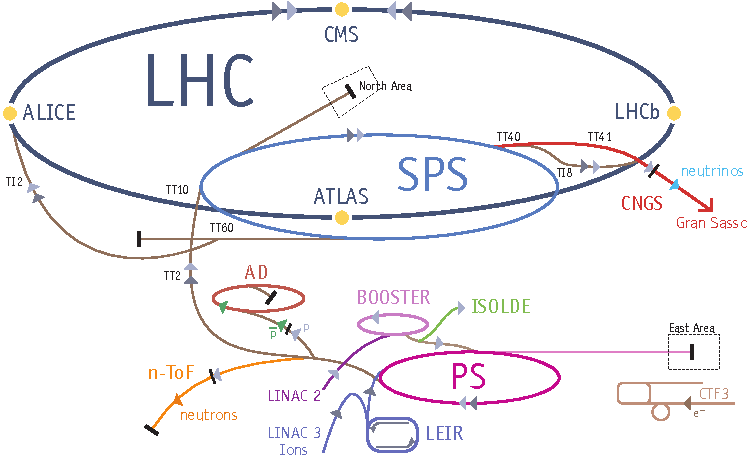
\includegraphics[width=.8\textwidth]{Cernrings}
\end{center}
\begin{minipage}[b]{\textwidth}
\caption{A schematic view of the \textsc{cern} accelerator complex \cite{cernbro}, in which protons or heavy ions used in collision experiments are accelerated through several machines to progressively higher energies. The paths protons can take through the machine are marked with light gray triangles. The dark gray triangles mark the paths taken by heavy ions when the Collider runs proton--lead or lead--lead collision experiments. Protons are `created' by ionising hydrogen atoms and then injected by \textcolor{Purple}{LINAC 2} into the \textcolor{Plum}{Booster ring}. From there, protons are accelerated by the Proton Synchrotron (\textcolor{Magenta}{PS}) and then the Super Protron Synchrotron (\textcolor{RoyalBlue}{SPS}) before finally being sent into the \textcolor{MidnightBlue}{LHC} ring. The LHC ring is the largest circular accelerator in the \textsc{cern} complex, and---at time of writing---in the world, measuring approximately 27~km in circumference.}
\label{cernrings}
\end{minipage}
\end{figure}

The \textsc{cern} accelerator complex comprises a number of particle accelerators with a wide variety of sizes, which service several experiments with various aims \cite{cernexps}. The most conspicuous element of the accelerator complex, of which an overview is given in figure~\ref{cernrings}, is the LHC ring, which is 27~km in circumference (which, even by the standards of particle accelerators, is quite large) and designed to contain proton (a species of hadron) beams with energies as high as 7~TeV. Where two such beams cross one another, proton collisions with 14~TeV energy may occur. The LHC's beams cross one another at four points around the ring, each one the site of one of the four main experiments.

The LHC is the last step in a series of particle accelerators---which incorporates two of \textsc{cern}'s previous main accelerators, the Proton Synchrotron and the Super Proton Synchrotron---which is needed to bring protons from rest to a final energy of 7~TeV. Throughout, protons are accelerated by applied electric fields, applied within so--called radiofrequency cavities, and contained within the rings by dipole magnets. Magnets with higher pole counts are used to manipulate the profile of the proton beam. [Fernow, maybe?]

Even though the LHC was designed for an energy per beam of 7~TeV, giving a collision energy of 14~TeV, several accidents during commissioning of the machine have necessitated the use of a lower beam energy for the first runs. In 2012, when the data that will be used in this thesis was taken, the LHC ran at 4~TeV per beam, for a total collision energy of 8~TeV.

Although we speak of proton beams, protons within the beams are arranged in discrete bunches, occurring at 50~ns intervals. As a consequence, proton collisions occur only within known time intervals, which dictate the timing by which detector readout occurs.

\section{The ATLAS detector}
The \textsc{atlas} detector is the largest of the LHC's four detector expermients, and is, as is the CMS\footnote{The \textbf{C}ompact \textbf{M}uon \textbf{S}olenoid.}, a general purpose detector, designed to capture as much information as possible about collision events. To that end, the \textsc{atlas} detector is made up of three distinct detector subsystems, layered concentrically about the interaction point, as illustrated in in figure~\ref{allatlas}. From innermost to outermost, these are: the tracking system, the calorimeter system and the muon spectrometer.

\begin{figure}[htp]
\begin{minipage}[b]{.69\textwidth}
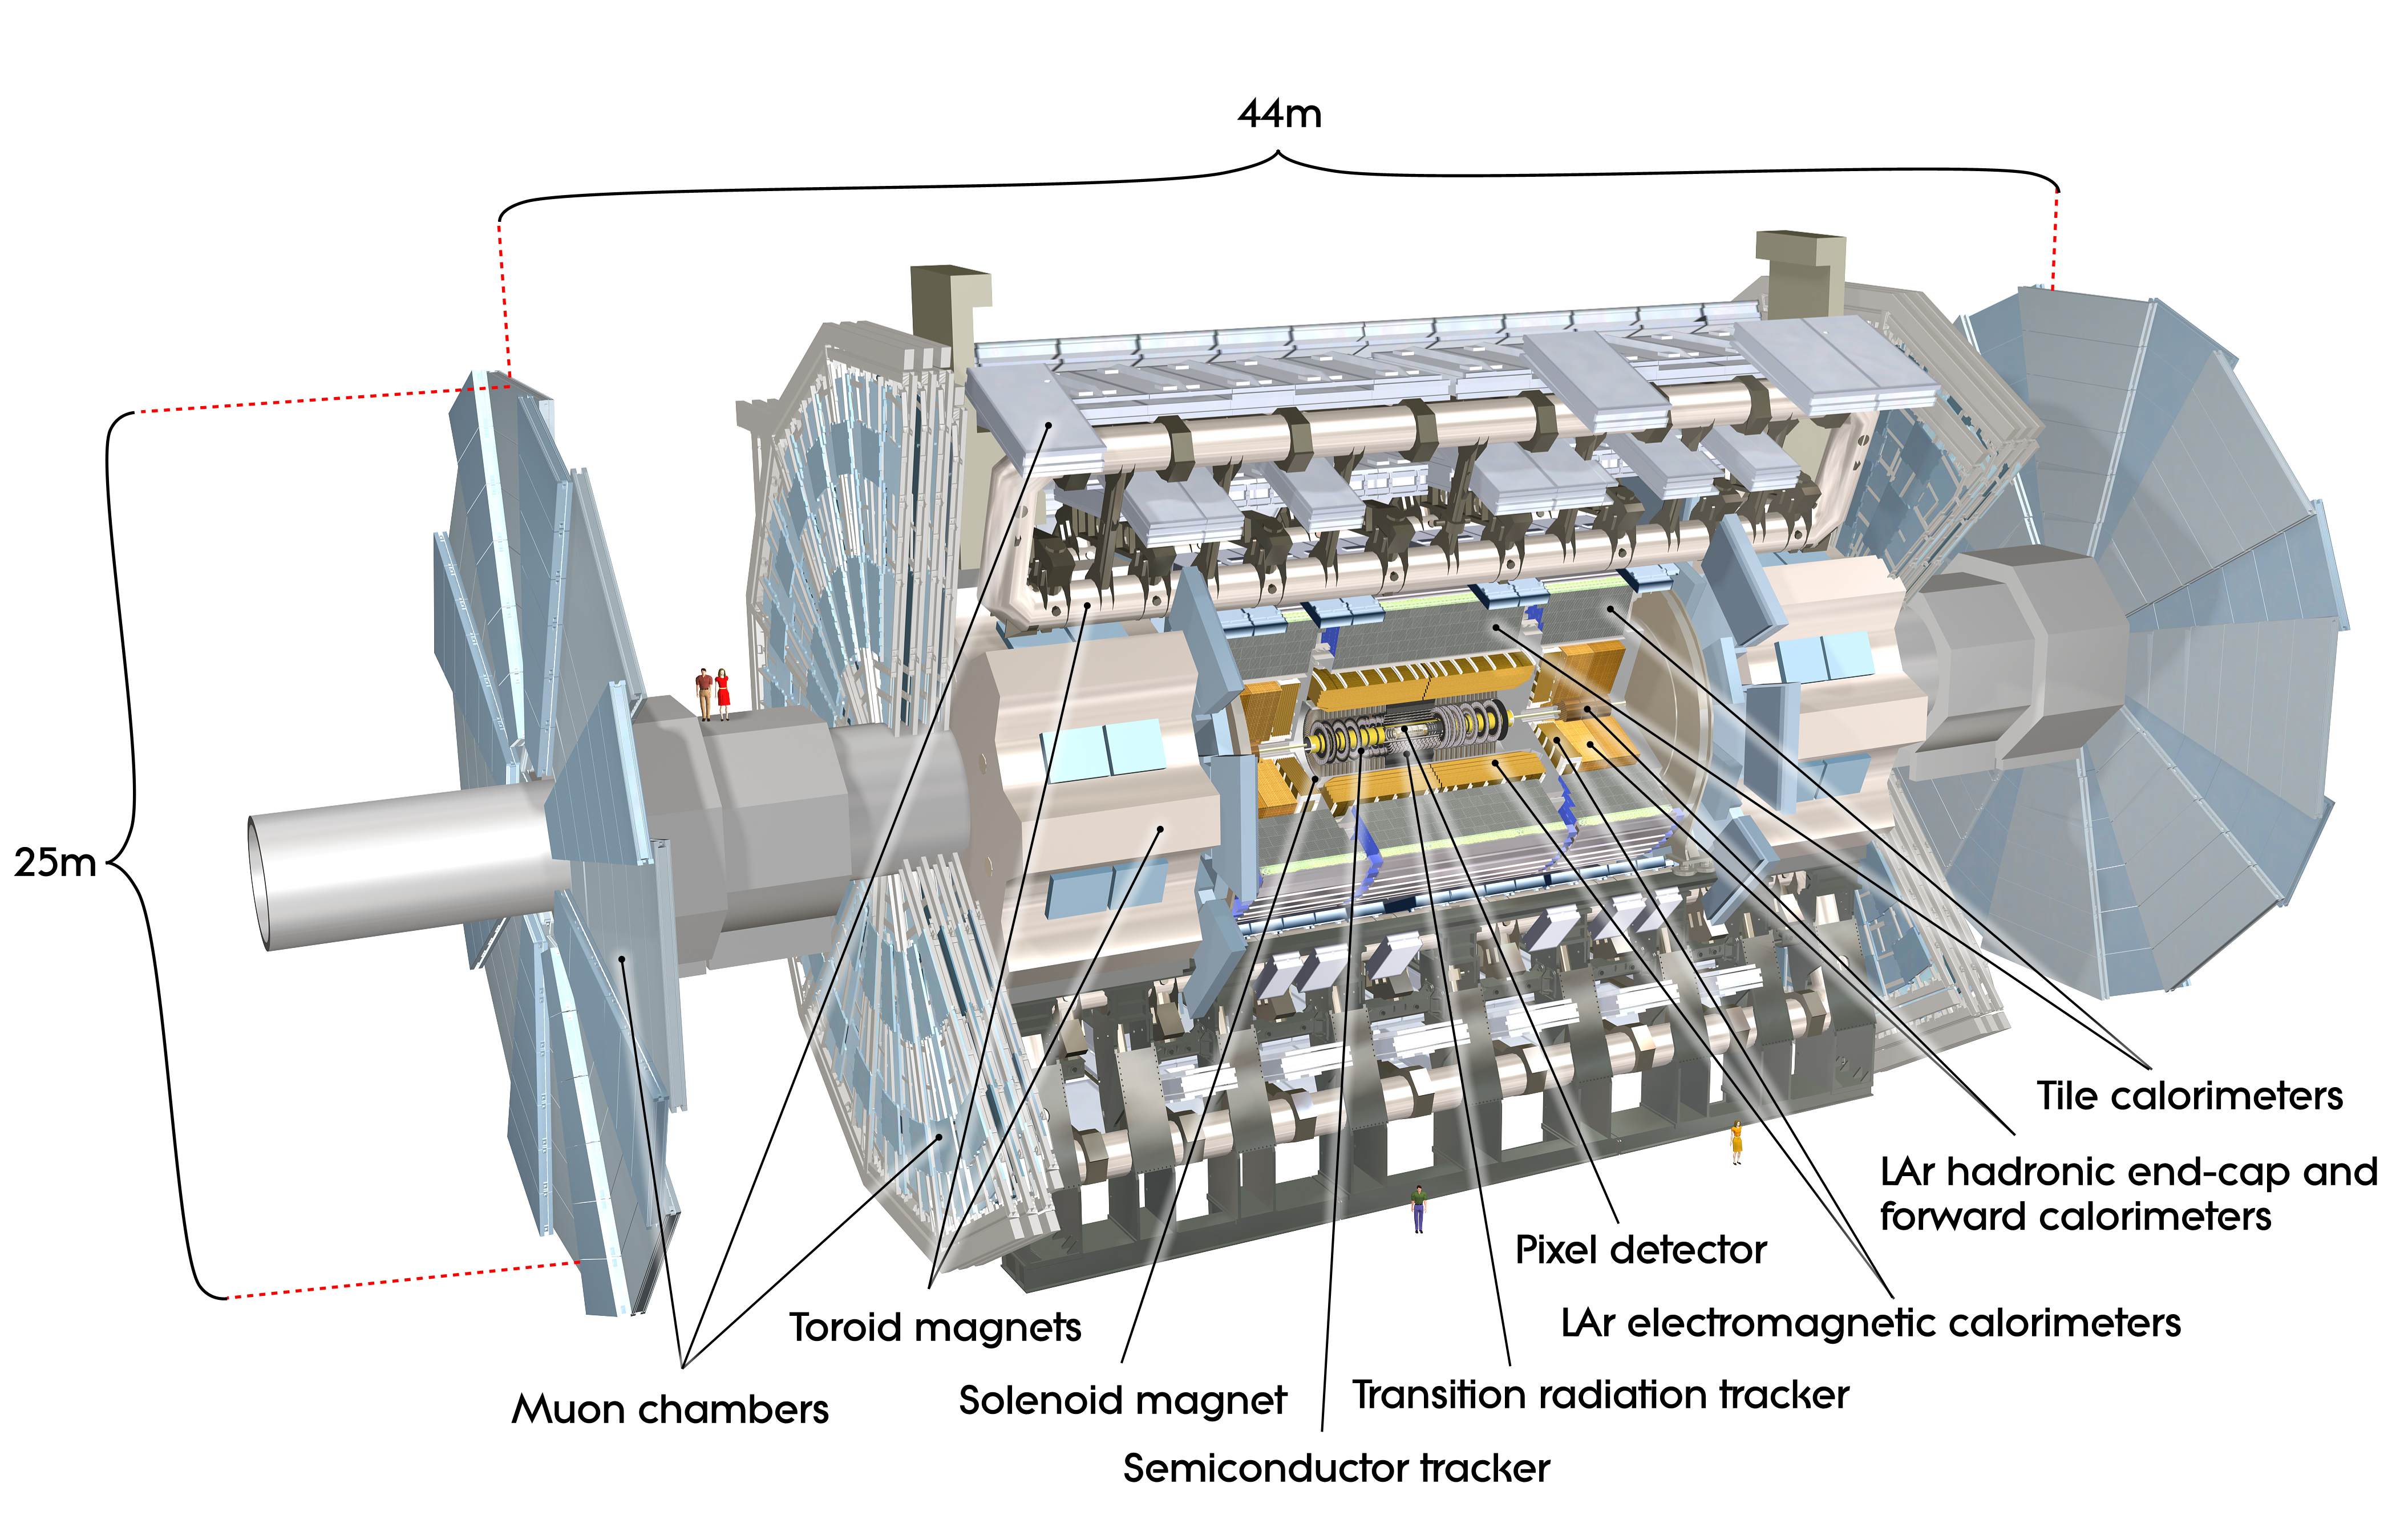
\includegraphics[width=1\textwidth]{AllAtlasBig}
\end{minipage}
\begin{minipage}[b]{.3\textwidth}
\caption{A diagram of the full \textsc{atlas} detector \cite{atlasweb}. The overall structure is of a layered cylinder centred on the interaction point. We refer to those parts of the detector that make up the wall of the cylinder as the barrel section, and to the ends of the cylinder as the endcap. The electromagnetic calorimeter, which is the detector element that we will make the most use of here, is coloured orange in this drawing.}
\end{minipage}
\label{allatlas}
\end{figure}

\textsc{Atlas} defines its own coordinate system, centred on the interaction point, where the position in the angular direction, perpendicular to the beam pipe, is measured by the azimuthal coordinate $\phi$, and the angle to the beam pipe is measured in pseudorapidity $\eta$, which is defined as
\(\eta\equiv-\ln[\tan(\theta/2)]=\half\ln\frac{|\mathbf{p}|+p_z}{|\mathbf{p}|-p_z},\)
where $\theta$ is the polar angle to the beam pipe in radians \cite{green}. The pseudorapidity $\eta$ is a simple transformation of $\theta$---it is 0 at $\theta=\pi/2$, $\infty$ at $\theta=0$ and $-\infty$ at $\theta=\pi$---but is chosen since it is approximately, and for massless particles exactly, equal to rapidity, 
\[ y \equiv \frac{1}{2} \ln \frac{E + p_z }{E - p_z }, \]
which is additive under Lorenz boosts in the $z$ direction \cite{green}.

A machine as large and complex as \atlas{} would require a large document, such as~\cite{detectorpaper}, to describe in comprehensive detail. For the present, a decidedly non-comprehensive description of the three detector layers, in order of increasing relevance to this work, follows.

The muon spectrometer forms the outermost, and most voluminous, part of the detector. As a species, muons, along with neutrinos, are the only types of particles that can regularly penetrate both calorimeters. Capturing neutrinos with \textsc{atlas}' mere 90\,000~t of material and 7\,000~m$^3$ detector volume \cite{atlasweb} is something of a lost cause, however.

The muon spectrometer and the inner detector are both tracking detectors, meaning that they are designed to determine the path of a charged particle that passes through them. By immersing such a detector in a magnetic field, which will deflect a charged particle, the charge sign and momentum of the particle can be deduced from the curvature of the track.

The inner detector is also a tracking detector, which uses two distinct detector technologies to localise the tracks of charged particles that pass through it. The innermost layers use silicon semiconductor chips to detect the charge left by a passing charged particle, essentially by allowing the ionisation charge to flip a transistor. The outer part of the inner detector uses drift straws, long tubes having a wire, which carries a high voltage charge, in the centre, filled with an inert gas. The ionisation charge left by a passing high--energy particle is attracted to the wire, and read out by detectors attached to its ends as a voltage change. The silicon detector is compact system with a high resolution, whereas the straw detectors can economically cover a large volume.

Both the straw detector and the outer part of the silicon detector---the silicon microstrip detector---have very long detector elements, which can only report that a hit has occurred somewhere along its length\footnote{Some additional resolution can be gained by studying the drift time in the straw detectors.}. To improve resolution in the long direction of these detectors, successive layers of detector elements are placed at an angle to one another, so that hits on successive detector elements narrow down the possible location of a track. The innermost layer of the silicon detector, the pixel detector, uses a pixel structure rather than a strip structure, and so has adequate resolution in all directions. What is worth noting here is that the tracking detector only directly reports times and---more or less approximate---locations of particle observations. They are only combined into particle tracks during a later analysis step. 

There are two calorimeter systems in \textsc{atlas}: the (inner) electromagnetic calorimeter and the (outer) hadronic calorimeter. In this context, a calorimeter is a device which attempts to absorb energetic particles in some material, and then measures the amount of energy deposited in the process. All calorimeters in \textsc{atlas} are sampling calorimeters, meaning that the absorbing material is divided into layers, with some form of detector inserted between the layers, which sample the flow of energy through the material at various depths. In the barrel section of the hadronic calorimeter---the tile calorimeter, the absorbing material is steel, and the sensitive layers are scintillators, a material that luminesces when exposed to ionising radiation. The light produced there is then guided to photomultipliers for detection.

The remaining calorimeters, which covers both the EM calorimeters and the endcap hadronic calorimeters, are all of a similar design, which has liquid argon as the sensitive material, and are thus called LAr calorimeters. As with the straw detectors, activity in the liquid argon layers are detected by an electrode, which picks up the ionisation left by passing energetic particles. In the barrel LAr calorimeters, the absorbing material is lead encased in thin steel layers. The endcap LAr calorimeters, however, are subjected to much stronger particle fluxes, and so copper, and in some cases tungsten, is used in place of lead, owing to their greater resistance to high temperatures.

\subsection{The electromagnetic calorimeter}

The EM calorimeters are particularly important tools for detecting photons. As such, we devote an entire sub--section to their description.

\begin{figure}[htp]
\begin{minipage}[b]{.69\textwidth}
\begin{infilsf}\footnotesize
\begin{tikzpicture}[x=\textwidth*.95/3.5,y=\textwidth*.95/3.5]

\tikzset{photon/.style={decorate,decoration={snake,amplitude=1}},
         vert/.style={fill=black,circle,draw,inner sep=0pt,minimum size=2},
         grid/.style={draw=kugray!50}
         }
         
\draw[grid] (0,-.6) -- +(0,1.5) (1,-.6) -- +(0,1.5) (2,-.6) -- +(0,1.5) (3,-.6) -- +(0,1.5);
\draw (-.2,-.6) -- (0,-.6) node[below] {0} -- +(0,.05) +(0,0) -- ++(1,0) node[below] {1} -- +(0,.05) +(0,0) -- ++(1,0) node[below] {2} -- +(0,0.05) +(0,0) -- ++(1,0) node[below] {3} -- +(0,.05) +(0,0) -- ++(.3,0);
\draw (3.2,-.6) +(0,-1.1em) node[below left] {Depth in radiation lengths};

\draw (-.1,0) -- (0.4,0) node[vert] {} -- (1.7,-.2) node[vert] {} -- (2.7,-0.1) node[vert] {} -- (3.2,0) ;
\draw[photon] (0.4,0) -- (1.3,.2) node[vert] {};
\draw (1.3,.2) -- node[above] {\tiny$+$} (2.5,.5) node[vert] {} -- node[below] {\tiny$+$} (3.2,.4);
\draw[photon] (2.5,.5) -- (3.2,.7);
\draw (1.3,.2) -- (2.3,.1) node[vert] {} -- (3.2,.2);
\draw[photon] (2.3,.1) -- (3.2,.05) (2.7,-.1) -- (3.2,-.1) (1.7,-.2) -- (2.3,-.3);
\draw (3.2,-.3) -- (2.3,-.3) node[vert] {} -- node[below] {\tiny$+$} (3.2,-.5);



\end{tikzpicture}
\end{infilsf}
\end{minipage}\hfill
\begin{minipage}[b]{.3\textwidth}
\caption{A schematic description of an EM shower developing in an absorbing material, adapted from \cite{fernow:sampcal}. Here, a wavy line indicates a photon, a straight line indicates an electron, and a straight line with a `$+$' a positron. At each split, the two resulting particles carry away half the energy of the original particle. In a sampling calorimeter, a sensitive layer is typically inserted at intervals of one radiation length. \textsc{Atlas}' LAr calorimeters measure the magnitude of ionisation that is left in the liquid argon by the passage of the particle shower.
\label{emshower}
}
\end{minipage}
\end{figure}

In the presence of matter, high--energy photons loose energy primarily through pair production, while electrons loose energy primarily through bremsstrahlung. The typical lengths travelled by both types of particle before undergoing these respective processes---their radiation lengths---depend on the material traversed, but are roughly equal to one another \cite{fernow:sampcal}. As illustrated in fig.~\ref{emshower}, both types of particles will undergo the same sort of evolution as they travel through an absorbing material, splitting into pairs of particles, each with a fraction of the energy of the parent particle, until the daughter particles no longer have sufficient energy to penetrate the absorbing material. Within the calorimeter, this cascade of particles forms a shower structure, an example of which is sketched in fig.~\ref{shower}. Thus, we can measure the energy of the original particle both by how deep into the absorbing material it penetrates, and by how many daughter particles it produces. In a homogeneous calorimeter, such as the one in CMS, where a single material is used both for absorbtion and detection, only the amount of activity produced by a hit to the calorimeter is measured. In a sampling calorimeter, where the absorbing material is passive, and activity is sampled by inserting sensitive layers into the absorbing material at intervals, can measure both the penetration depth, since the thickness of absorbing material in front of the deepest activated sensitive layer is known, and showering activity, by using proportional detectors in the sensitive layers. The radiation length is then a natural scale for the thickness of each layer of absorber. In total, the electromagnetic calorimeter has a thickness of at least 22 radiation lengths.

\begin{figure}[htp]
\begin{minipage}[t]{.4\textwidth}
\caption{Several figures, from \cite{atlasweb}, that illustrate the structure and use of the LAr calorimeters. These are sampling calorimeters, which have an absorbing medium (primarily lead and steel) with layers of detecting medium (liquid argon) inserted regularly to measure particle flux. In \textsc{atlas}' LAr calorimeters, rather than having flat layers, the absorbing and sensitive materials are interleaved in an accordion shape, visible in \subcaptionref{larpic} and \subcaptionref{shower}, which allows the detector electronics to be inserted along the gaps between the absorbing plates. Thus, the calorimeters do not need to be interrupted by non--sensitive space for signalling connections.}
\end{minipage}\hfill\begin{minipage}[t]{.57\textwidth}
\phantom{p}

\phantom{p}

    \begin{center}
    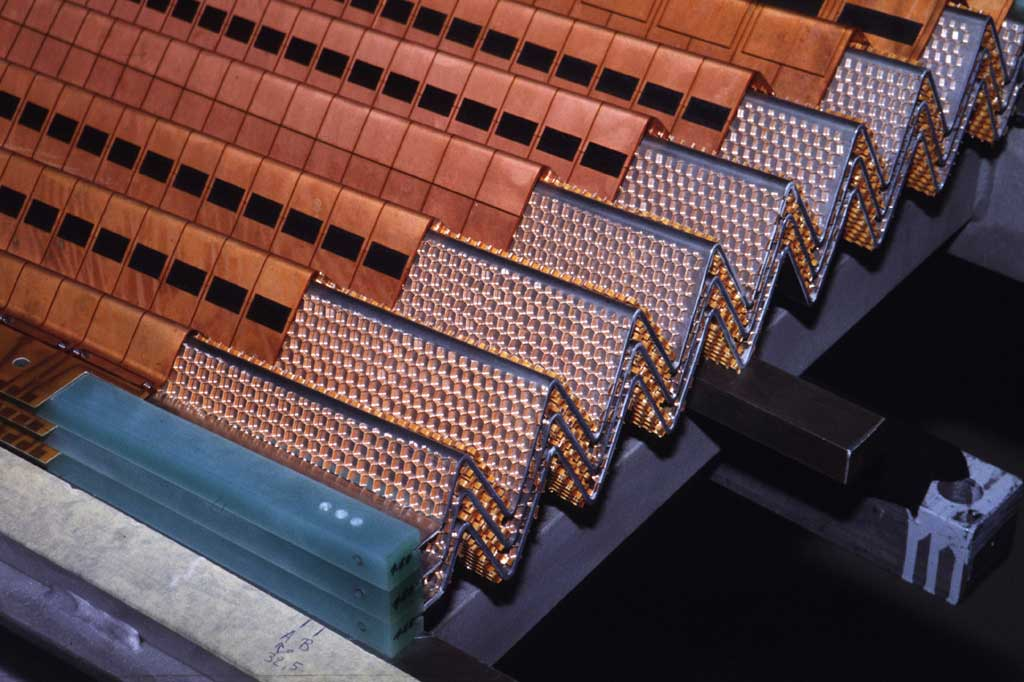
\includegraphics[width=\textwidth]{larpic}\makebox[0em][r]{\textcolor{natgreen}{\rule{\textwidth}{1pt}}}
    
    \subcaption{A section of the LAr calorimeter. \label{larpic}}
    \end{center}
\end{minipage}

\noindent\begin{minipage}[b]{.4\textwidth}
\begin{center}
    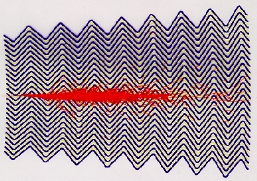
\includegraphics[width=\textwidth]{shower}\makebox[0em][r]{\textcolor{natgreen}{\rule{\textwidth}{1pt}}}

    \contsubcaption{Illustration of a particle shower within the LAr calorimeter. \label{shower}}
    \end{center}
\end{minipage}\hfill\begin{minipage}[b]{.57\textwidth}

    \begin{center}    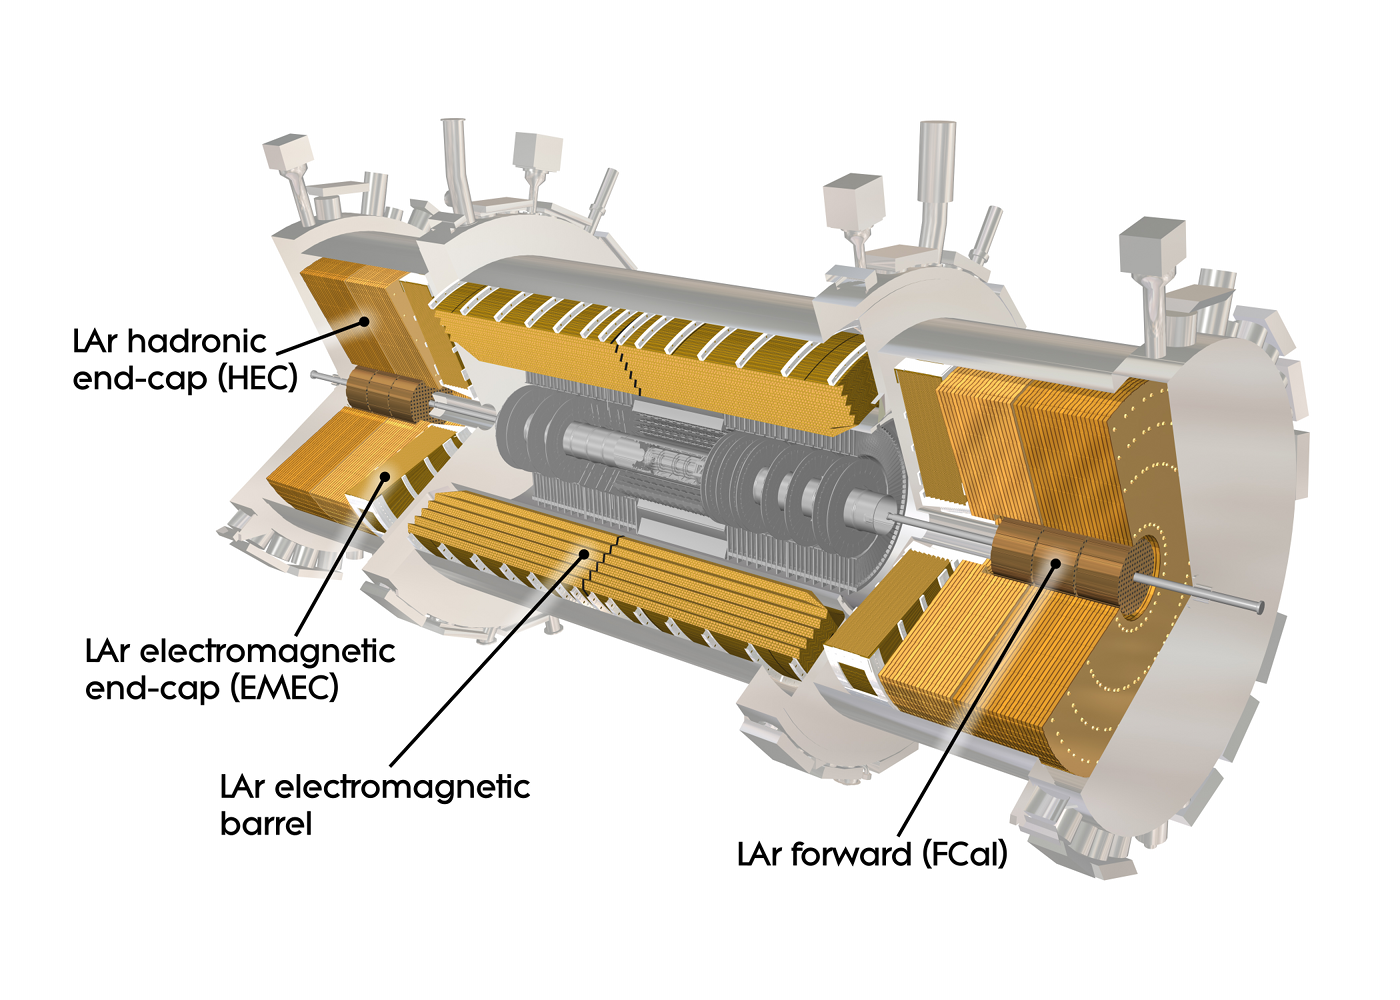
\includegraphics[width=1\textwidth]{figures/CaloDiag.png}
    \contsubcaption{Schematic showing the placement of the LAr calorimeters in \textsc{atlas}.}
    \end{center}
\end{minipage}
\label{calostruc}
\end{figure}

\Atlas{}' barrel LAr calorimeters are divided into three layers, which are split into readout bins as illustrated in fig.~\ref{caldiv}. The first layer is very finely divided in the $\eta$ direction, and its readout cells will on occasion be referred to as `strips' in the `strip layer', as opposed to the `cells' in the other two layers. The detectors function on the same sort of principle as the straw detectors in the inner detector: charged particles leave ionisation trails in the liquid argon, which is picked up on plates suspended in the middle of the LAr gap, which carry a high voltage charge. Each cell functions as a single proportional counter. Thus, the amount of energy deposited in each cell of each layer of the calorimeter is measured by the amount of showering activity in the sensitive layers of that cell.

\begin{figure}[htp]
\begin{minipage}[b]{.69\textwidth}
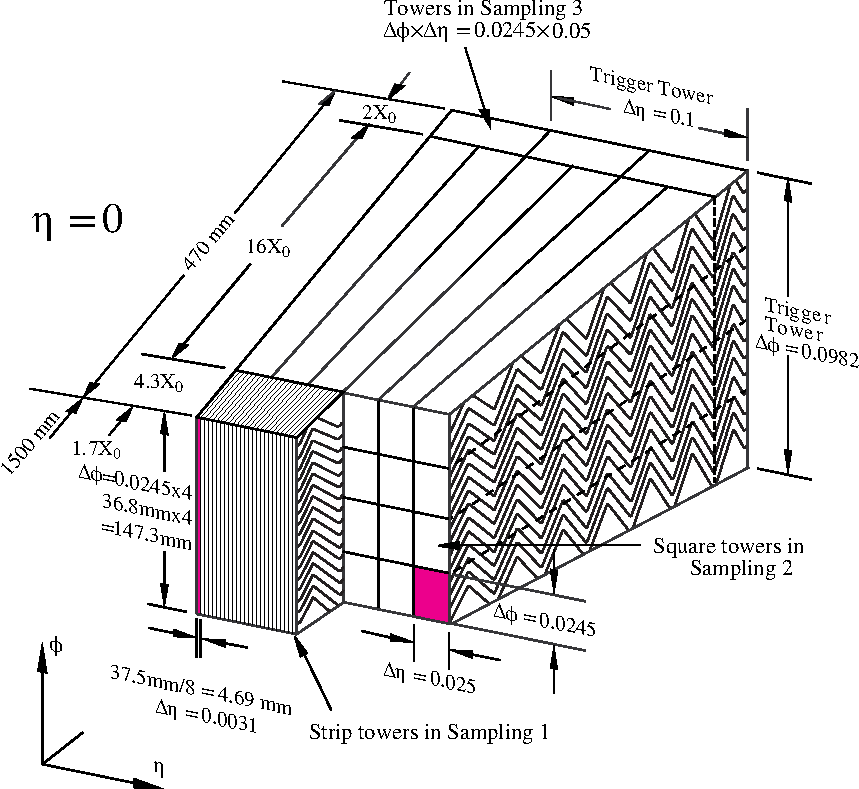
\includegraphics[width=\textwidth]{caldiv}
\end{minipage}
\begin{minipage}[b]{.3\textwidth}
\caption{The division of the EM calorimeter into detecting cells \cite{egede}. The first layer is divided into thin strips for the greatest resolution in the $\eta$ direction. The second layer is divided into roughly square cells, and comprises the bulk of the depth of the detector. The last layer is presumed to only be reached by the most energetic particles, and can have a coarser division without loosing resolution. This diagram is of the calorimeter at $\eta = 0$, closest to the interaction point. At higher $|\eta|$, the towers are angled so that they are still pointed toward the interaction point.
\label{caldiv}}
\end{minipage}
\end{figure}

The absorbing material in the barrel LAr calorimeter are accordion shaped sheets of lead held in iron sheets, visible in fig.~\ref{calostruc}, inserted radially into the detector, so that radiation leaving the detector is still faced with broadly uniform layers of absorbing material, while gaps between them, which are filled with liquid argon and hold the detector plates, still run contiguously throughout the depth of the calorimeter. Connections between the detectors in the inner part of the calorimeter and the readout electronics outside the calorimeter can be run through these gaps without needing to create holes in the detectors coverage.

The division of the calorimeter into layers gives us some resolution in depth when attempting to ascertain the shape of a shower. Showers initiated by types of particles other than photons or electrons evolve in a slightly different way, which allows us discern the source of a shower by examining its shape. Additionally, with this shower shape information, we can extrapolate the direction from which a particle entered the calorimeter, which is of particular importance when attempting to trace the origin of unconverted photons, which otherwise leave no trail in the detector.

There is quite a bit of material between the calorimeter and the interaction point, which is not part of the active detector systems, but may interact with a particle in the same way as the absorbing material in the calorimeter. To attempt to correct for this upstream energy loss, the first active layer, called the presampler, sits ahead of the first absorbing layer. Photons that undergo pair production sufficiently deep in the detector for the tracker to resolve at least one of the resulting (anti--)electrons are treated as a separate object type, namely converted photons. Identifying all the detector signatures that may have been left by photons is the first major (relevant) step in analysing the detector's output.

\subsection{Triggering and readout}
While in full operation for the 2012, 8~TeV run, the LHC delivered a bunch crossing in \textsc{atlas}' interaction point every 50~ns, or 20 million bunch crossings per second. Reading out the whole detector produces 1.6~MB of information, which, if the detector were read out completely with every crossing, would produce a data rate of 34~TB/s.\footnote{For perspective, that is approximately equal to the estimated global IP traffic rate in 2015, according to \cite{wolframip}.} However, since only a fraction of these crossings will contain interesting physics events, we can reduce the data rate to less prohibitive levels simply by not recording data from collision that do not produce interesting outcomes. To accomplish this, we need a system that examines events in the detector as they occur, and trigger recording whenever it sees an interesting event. In \textsc{atlas}, this trigger system has three levels, which are described in detail in \cite{detectorpaper}. 

The level--1 trigger examines detector output in real time. To do so, the trigger logic is run on specialised hardware built in to the detectors themselves. As a result, each trigger only has access to information from the detector its hardware is attached to. Calorimeter triggers, for example, do not have access to information from the tracking system at the first trigger level. Also, computationally intensive tasks, such as track reconstruction, can not be completed in the window of time available to the level--1 trigger, and so are also not available. If a level--1 trigger fires, readouts from every detector element taken during the time window associated with that buch crossing are passed to the next trigger level, level--2. This trigger is run on the full set of temporarily stored information from an event, on those events which pass the level--1 filter. The final trigger level works with fully reconstructed events and derived physical observables. This requires more time and processing power than is available at the previous levels, but it also identifies interesting events with the same quality of information as will be used in the subsequent analysis. All three triggers in combination cuts the final event rate to 300 events per second, with a peak rate of 600 events.

For this thesis, we shall use data taken during the 8~TeV run in 2012. The amount of data taken at any given time depends on the conditions of the beam, which can be summarised in the instantaneous luminosity, and the conditions of the detector, which may only capture a fraction of the events produced at any given time. Figure~\ref{intlumi} gives the distribution of integrated and captured luminosity over the course of the year.

\begin{figure}[htp]
\begin{minipage}[b]{.57\textwidth}
\hspace{-1em}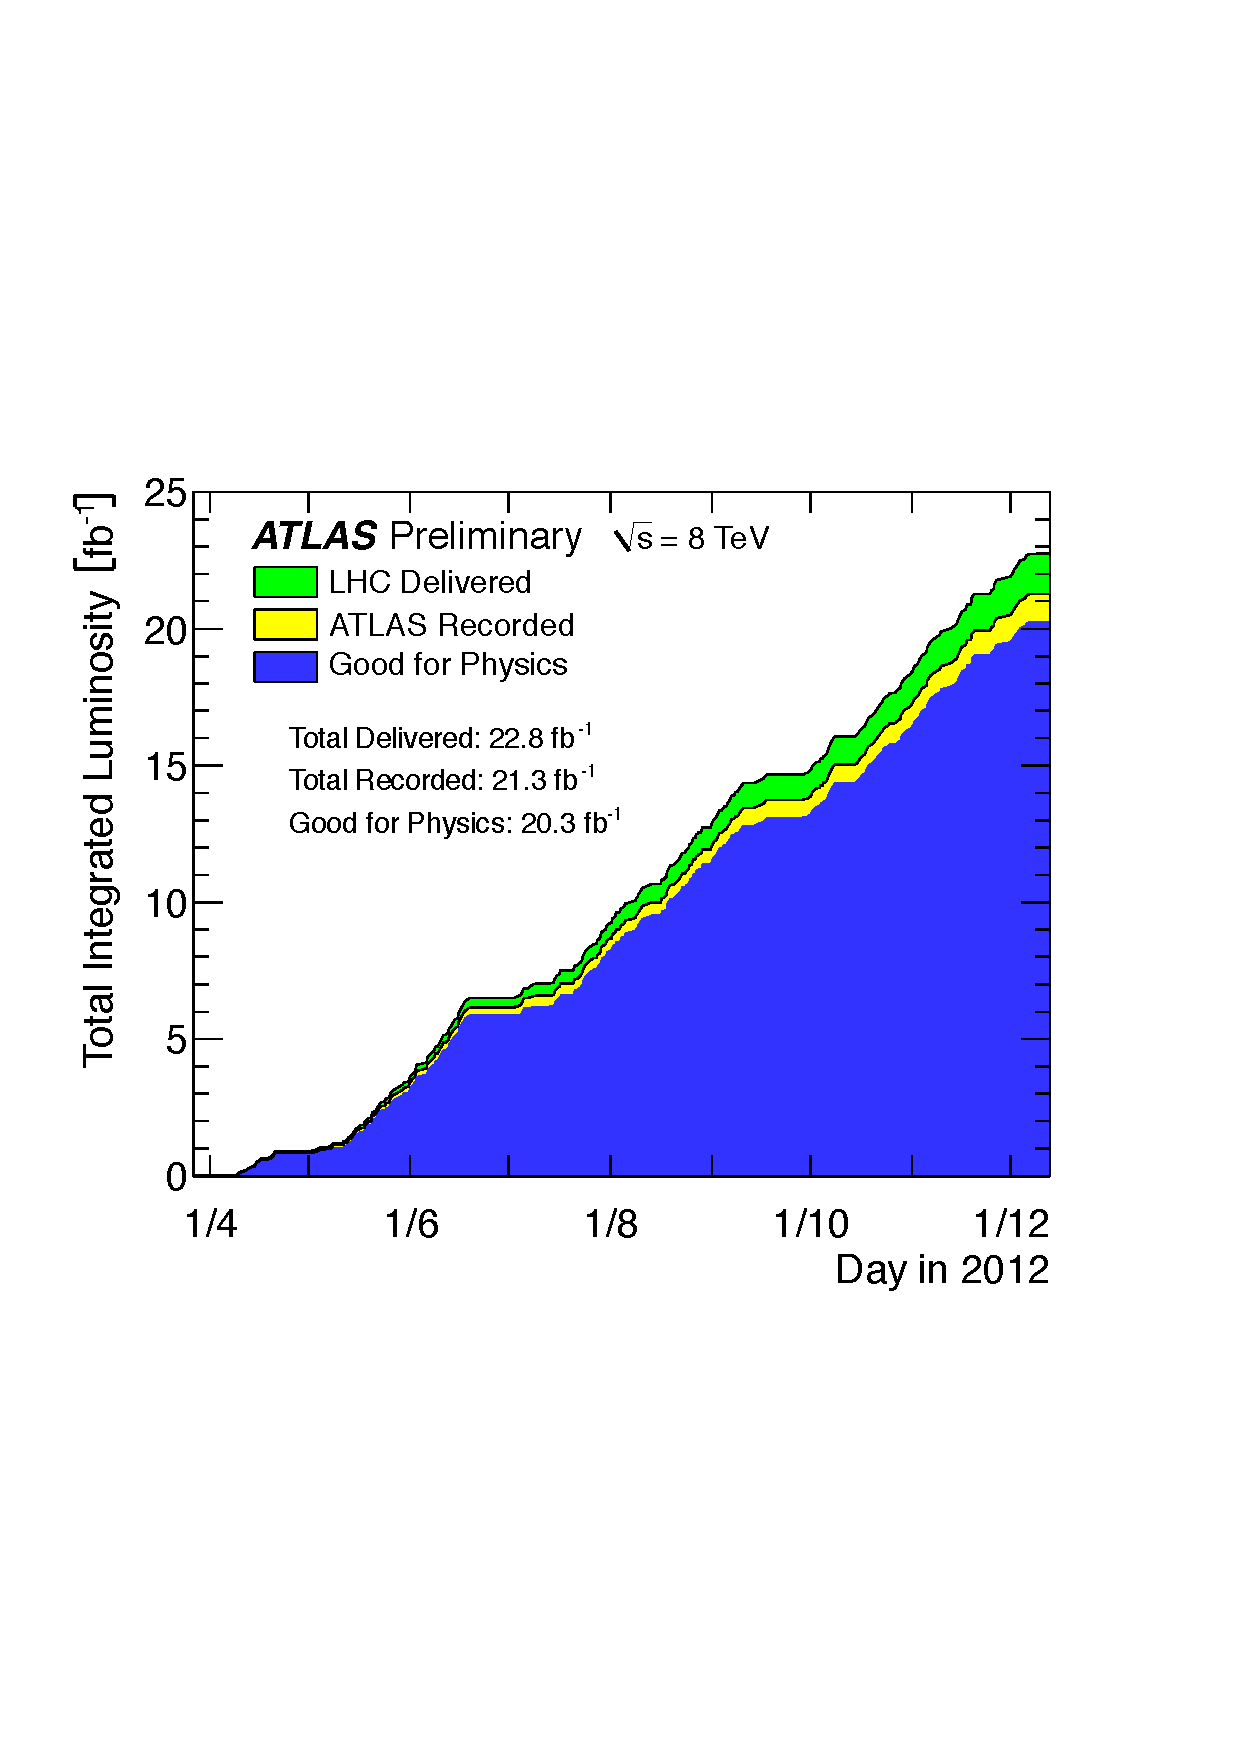
\includegraphics[width=\textwidth]{figures/intlumi}
\end{minipage}\hfill\begin{minipage}[b]{.4\textwidth}
\caption{A plot \cite{publiclumi} showing the integrated luminosity delivered by the LHC (green), recorded by \atlas{} (yellow), and fulfilling data quality criteria (blue), over the course of the 8 TeV run in 2012.
\label{intlumi}}
\end{minipage}
\end{figure}

Unfortunately, the triggers that are implemented in \atlas{} do not guarantee that the readout rate remains within the technical limitations of the readout system. To stay within those limits, a prescale is applied to triggers that select more collision events than it is considered worth keeping,\footnote{Explaining how worth is assigned to event types is not a topic within the scope of this thesis.} which means simply that a fraction of collisions that pass a trigger are not recorded. The diphoton channel is important to the search for the Higgs boson, however, so, fortunately, no prescales have been applied to the triggers that produce diphotons events.

For this thesis, we will be working with data prepared by \atlas{}s e/gamma working group, which has defined the final reconstruction procedures, as well as final requirements on data quality and detector status. After these requirements are applied, the 20.3 fb$^{-1}$ of data generated by the \atlas{} detector is reduced to 18.301 fb$^{-1}$, available in the {\texttt NTUP\_PHOTON} format.


\subsection{Photon identification}
In broad terms, we may view information coming from the detector in terms of energy clusters in the calorimeters or tracks in the inner detector. Assigning calorimeter deposits to discrete clusters is a task that can be approached a number of ways, both subtle and complex, however at the low--level trigger stage, the straightforward sliding window method is used \cite{atlascluster:sw}. A rectangle of fixed size is defined by combining calorimeter cells, and the energy within is summed. This `window' is then `slid' across the entire calorimeter, and a cluster candidate is proclaimed whenever the energy within the window reaches a local maximum above a predefined threshold value.

Assuming that every charged particle leaves both a track in the inner detector and a cluster in the calorimeter, we interpret every cluster in the calorimeter that can not be associated with a track as the signature of a neutral particle. Each of these neutral particles might be an unconverted photon, and so every cluster without an associated track is added to the list of photon candidates.

As previously mentioned, converted photons are photons that undergo pair production ``in flight.'' As such, we expect the detector signature of such events to be a positively and a negatively charged track with a common vertex away from the interaction point. Any set of measurements that match this signature may be added to the sequence straight away, however since track reconstruction is an imperfect process, especially in the straw detector, we include also any electron candidate, whose track is reconstructed solely from hits in the straw detector.

These steps form a selection algorithm, which creates a list of photon candidates for every bunch crossing in \atlas{} \cite{phorec}.

This set will of course contain many events that were not photons: $\pi^0$ mesons also create calorimeter hits with no associated track, and QCD jets can mimic converted photons, among other possibilities. To attempt to sort genuine photon events from impostor events, we study the shape of the shower left in the calorimeter. To that end, we define the following shower shape variables:

\begin{itemize}
\item $R_\text{had}$, the ratio of energy deposited in the hadronic calorimeter to the cluster energy in the EM calorimeter. Hadronic showers are expected to penetrate deeper into the hadronic calormieter than EM showers.
\item In the middle EM calorimeter layer, non-EM showers spread wider than electromagnetic ones. The variables that measure the shape of the shower in this layer are:
\begin{itemize}
\item $R_\eta$, the ratio in $\eta$ of cell energies in 3 $\times$ 7 versus 7 $\times$ 7 cells.
\item $R_\phi$, the ratio in $\phi$ of cell energies in 3 $\times$ 7 versus 7 $\times$ 7 cells.
\item $w_{\eta 2}$, the width of the shower in the $\eta$ direction.
\end{itemize}
\item The strip layer, with its greater resolution in $\eta$, can pick out some of the internal structure of a jet. Hadron showers tend to show more than one maximum. Variables that measure the shape in the strip layer are:
\begin{itemize}
\item $w_{s3}$, the shower width for three strips around the maximum strip.
\item $w_{s\text{ tot}}$, the total lateral shower width in the strip layer.
\item $F_\text{side}$, the faction of energy deposited outside a core of 3 central strips, but within 7 strips.
\item $\Delta E$, the difference in energy of the strip with the second largest energy deposited and the strip with the smallest energy deposited between the two leading strips.
\item $E_\text{ratio}$, the ratio of the energy difference associated with the
largest and second largest energy deposits, over the sum of these energies.
\end{itemize}
\end{itemize}

Converted and unconverted photons will of course have different signatures in these variables. Thus, the photon identification algorithm also includes a step which calibrates and corrects the detector response to these two object categories \cite{phorec}.

Cuts made in these variables form the selection criteria that are used to divide the sample of photon candidates into those that are to be considered actual or impostor photons. The full list of variables above forms the tight selection criteria, while a shorter list, consisting of $R_\text{had}$, $R_\eta$ and $w_{\eta2}$ form the loose selection criteria. Separate cut values in these variables exist for different $\eta$ ranges. A complete description is available in \cite{Carminati}.

\section{Detector simulation}
In chapter~\ref{ch.mc}, we employed Monte Carlo techniques to simulate the outcome of the processes we wish to study. From this procedure, we retain perfect knowledge of every step in the evolution of those events. This is very unlike the picture that the detector will give us of the events in the actual, physical experiment.

The actual events will be viewed through the `lens' of the \atlas{} detector. The detector only registers changes in voltage in its individual detector elements. The objects that analyses such as this will deal with---tracks, energy clusters and jets---are reconstructed from the raw reading in individual detector elements by computer algorithms\footnote{This summary of the \atlas{} detector will be expanded upon in chapter~\ref{ch.exp}.}. Additionally, the final state particles produced by the hard process, as simulated by pythia, could potentially interact with the material that makes up the detector and decay, split or convert before or during their detection, while the detector does not fully or accurately detect all the particles that pass through it. Because of this, it is necessary to also simulate how the detector interacts with the final state particles we generated in the previous section, to properly relate that information with experimental data.

Furthermore, as discussed above, the collisions that the LHC produces are not between single protons, but between bunches containing of the order 10$^{11}$ protons \cite{cernbro}, which follow one another at 50 ns intervals. Because of this, particles produced by more than one proton collision will be present within the \atlas{} detector during the recording window for each bunch crossing, either from multiple protons in the current bunches interacting, or from the products of the previous or subsequent bunches intruding into the recording window. For the period in question, the average number of interactions per crossing easily exceeds 20 \cite{publiclumi}. Collectively, we refer to these---for our purposes---extraneous events as pileup. The solution for reproducing the effects of pileup in simulated events is to randomly pick an appropriate number of generic pileup events from a dedicated set of simulated events, and add them on top of the interesting event, to approximate the complete product of a collision in the detector. Since the distribution of numbers of interaction to be added per event were specified before the 8~TeV run was completed, the expected distribution does not match the measued one exactly. To account for the difference, Monte Carlo events are reweighted by their number of interactions to correct for this deviation~\cite{pileuprew}.

Since these steps must be followed every time a Monte Carlo set that approximates the \atlas{} experiment is produced, the information and computer programs needed to run them are provided in a standard package by the \atlas{} Collaboration. The simulation of the interaction between particles and the physical detector comes in the form of a geometry model for \textsc{geant4}, a program that can simulate the interaction between high--energy particles and matter.

The real detector has a finite energy resolution, which is not reflected in the Monte Carlo events, for which we have an exact momentum. To overcome this, we smear the energies given by the simulation---that is shift the energies by a random amount chosen from a gaussian distribution with a width chosen to reflect the resolution of the detector~\cite{ecalib}.

The effect that the detector simulation has on the invariant mass distribution of the event samples created above is shown in figure~\ref{geant-beaf}.

\begin{figure}[htp]
\begin{minipage}[b]{.69\textwidth}
\begin{infilsf} \tiny
\pgfdeclareplotmark{cross} {
\pgfpathmoveto{\pgfpoint{-0.3\pgfplotmarksize}{\pgfplotmarksize}}
\pgfpathlineto{\pgfpoint{+0.3\pgfplotmarksize}{\pgfplotmarksize}}
\pgfpathlineto{\pgfpoint{+0.3\pgfplotmarksize}{0.3\pgfplotmarksize}}
\pgfpathlineto{\pgfpoint{+1\pgfplotmarksize}{0.3\pgfplotmarksize}}
\pgfpathlineto{\pgfpoint{+1\pgfplotmarksize}{-0.3\pgfplotmarksize}}
\pgfpathlineto{\pgfpoint{+0.3\pgfplotmarksize}{-0.3\pgfplotmarksize}}
\pgfpathlineto{\pgfpoint{+0.3\pgfplotmarksize}{-1.\pgfplotmarksize}}
\pgfpathlineto{\pgfpoint{-0.3\pgfplotmarksize}{-1.\pgfplotmarksize}}
\pgfpathlineto{\pgfpoint{-0.3\pgfplotmarksize}{-0.3\pgfplotmarksize}}
\pgfpathlineto{\pgfpoint{-1.\pgfplotmarksize}{-0.3\pgfplotmarksize}}
\pgfpathlineto{\pgfpoint{-1.\pgfplotmarksize}{0.3\pgfplotmarksize}}
\pgfpathlineto{\pgfpoint{-0.3\pgfplotmarksize}{0.3\pgfplotmarksize}}
\pgfpathclose
\pgfusepathqstroke
}
\pgfdeclareplotmark{cross*} {
\pgfpathmoveto{\pgfpoint{-0.3\pgfplotmarksize}{\pgfplotmarksize}}
\pgfpathlineto{\pgfpoint{+0.3\pgfplotmarksize}{\pgfplotmarksize}}
\pgfpathlineto{\pgfpoint{+0.3\pgfplotmarksize}{0.3\pgfplotmarksize}}
\pgfpathlineto{\pgfpoint{+1\pgfplotmarksize}{0.3\pgfplotmarksize}}
\pgfpathlineto{\pgfpoint{+1\pgfplotmarksize}{-0.3\pgfplotmarksize}}
\pgfpathlineto{\pgfpoint{+0.3\pgfplotmarksize}{-0.3\pgfplotmarksize}}
\pgfpathlineto{\pgfpoint{+0.3\pgfplotmarksize}{-1.\pgfplotmarksize}}
\pgfpathlineto{\pgfpoint{-0.3\pgfplotmarksize}{-1.\pgfplotmarksize}}
\pgfpathlineto{\pgfpoint{-0.3\pgfplotmarksize}{-0.3\pgfplotmarksize}}
\pgfpathlineto{\pgfpoint{-1.\pgfplotmarksize}{-0.3\pgfplotmarksize}}
\pgfpathlineto{\pgfpoint{-1.\pgfplotmarksize}{0.3\pgfplotmarksize}}
\pgfpathlineto{\pgfpoint{-0.3\pgfplotmarksize}{0.3\pgfplotmarksize}}
\pgfpathclose
\pgfusepathqfillstroke
}
\pgfdeclareplotmark{newstar} {
\pgfpathmoveto{\pgfqpoint{0pt}{\pgfplotmarksize}}
\pgfpathlineto{\pgfqpointpolar{44}{0.5\pgfplotmarksize}}
\pgfpathlineto{\pgfqpointpolar{18}{\pgfplotmarksize}}
\pgfpathlineto{\pgfqpointpolar{-20}{0.5\pgfplotmarksize}}
\pgfpathlineto{\pgfqpointpolar{-54}{\pgfplotmarksize}}
\pgfpathlineto{\pgfqpointpolar{-90}{0.5\pgfplotmarksize}}
\pgfpathlineto{\pgfqpointpolar{234}{\pgfplotmarksize}}
\pgfpathlineto{\pgfqpointpolar{198}{0.5\pgfplotmarksize}}
\pgfpathlineto{\pgfqpointpolar{162}{\pgfplotmarksize}}
\pgfpathlineto{\pgfqpointpolar{134}{0.5\pgfplotmarksize}}
\pgfpathclose
\pgfusepathqstroke
}
\pgfdeclareplotmark{newstar*} {
\pgfpathmoveto{\pgfqpoint{0pt}{\pgfplotmarksize}}
\pgfpathlineto{\pgfqpointpolar{44}{0.5\pgfplotmarksize}}
\pgfpathlineto{\pgfqpointpolar{18}{\pgfplotmarksize}}
\pgfpathlineto{\pgfqpointpolar{-20}{0.5\pgfplotmarksize}}
\pgfpathlineto{\pgfqpointpolar{-54}{\pgfplotmarksize}}
\pgfpathlineto{\pgfqpointpolar{-90}{0.5\pgfplotmarksize}}
\pgfpathlineto{\pgfqpointpolar{234}{\pgfplotmarksize}}
\pgfpathlineto{\pgfqpointpolar{198}{0.5\pgfplotmarksize}}
\pgfpathlineto{\pgfqpointpolar{162}{\pgfplotmarksize}}
\pgfpathlineto{\pgfqpointpolar{134}{0.5\pgfplotmarksize}}
\pgfpathclose
\pgfusepathqfillstroke
}
\begin{tikzpicture}[x=.054\textwidth,y=.054\textwidth]
\definecolor{c}{rgb}{1,1,1};
\draw [color=c, fill=c] (0,0) rectangle (17.5689,26);
\draw [color=c, fill=c] (0,15.3878) rectangle (17.5689,26);
\draw [color=c, fill=c] (1.75689,15.3878) rectangle (15.812,24.9388);
\definecolor{c}{rgb}{0,0,0};
\draw [c] (1.75689,15.3878) -- (1.75689,24.9388) -- (15.812,24.9388) -- (15.812,15.3878) -- (1.75689,15.3878);
\definecolor{c}{rgb}{1,1,1};
\draw [color=c, fill=c] (1.75689,15.3878) rectangle (15.812,24.9388);
\definecolor{c}{rgb}{0,0,0};
\draw [c] (1.75689,15.3878) -- (1.75689,24.9388) -- (15.812,24.9388) -- (15.812,15.3878) -- (1.75689,15.3878);
\colorlet{c}{kugray}
\draw [c] (1.89744,24.6327) -- (1.89744,24.6349);
\draw [c] (1.89744,24.6349) -- (1.89744,24.6371);
\draw [c] (1.75689,24.6349) -- (1.89744,24.6349);
\draw [c] (1.89744,24.6349) -- (2.038,24.6349);
\draw [c] (2.17855,23.6447) -- (2.17855,23.6509);
\draw [c] (2.17855,23.6509) -- (2.17855,23.6571);
\draw [c] (2.038,23.6509) -- (2.17855,23.6509);
\draw [c] (2.17855,23.6509) -- (2.3191,23.6509);
\draw [c] (2.45965,22.9779) -- (2.45965,22.9906);
\draw [c] (2.45965,22.9906) -- (2.45965,23.0029);
\draw [c] (2.3191,22.9906) -- (2.45965,22.9906);
\draw [c] (2.45965,22.9906) -- (2.6002,22.9906);
\draw [c] (2.74075,22.4884) -- (2.74075,22.5096);
\draw [c] (2.74075,22.5096) -- (2.74075,22.5299);
\draw [c] (2.6002,22.5096) -- (2.74075,22.5096);
\draw [c] (2.74075,22.5096) -- (2.8813,22.5096);
\draw [c] (3.02186,22.1055) -- (3.02186,22.1374);
\draw [c] (3.02186,22.1374) -- (3.02186,22.1672);
\draw [c] (2.8813,22.1374) -- (3.02186,22.1374);
\draw [c] (3.02186,22.1374) -- (3.16241,22.1374);
\draw [c] (3.30296,21.7749) -- (3.30296,21.8201);
\draw [c] (3.30296,21.8201) -- (3.30296,21.8613);
\draw [c] (3.16241,21.8201) -- (3.30296,21.8201);
\draw [c] (3.30296,21.8201) -- (3.44351,21.8201);
\draw [c] (3.58406,21.3741) -- (3.58406,21.4431);
\draw [c] (3.58406,21.4431) -- (3.58406,21.5033);
\draw [c] (3.44351,21.4431) -- (3.58406,21.4431);
\draw [c] (3.58406,21.4431) -- (3.72461,21.4431);
\draw [c] (3.86516,21.0342) -- (3.86516,21.1331);
\draw [c] (3.86516,21.1331) -- (3.86516,21.2148);
\draw [c] (3.72461,21.1331) -- (3.86516,21.1331);
\draw [c] (3.86516,21.1331) -- (4.00572,21.1331);
\draw [c] (4.14627,20.6175) -- (4.14627,20.7708);
\draw [c] (4.14627,20.7708) -- (4.14627,20.8864);
\draw [c] (4.00572,20.7708) -- (4.14627,20.7708);
\draw [c] (4.14627,20.7708) -- (4.28682,20.7708);
\draw [c] (4.42737,20.6944) -- (4.42737,20.7814);
\draw [c] (4.42737,20.7814) -- (4.42737,20.8548);
\draw [c] (4.28682,20.7814) -- (4.42737,20.7814);
\draw [c] (4.42737,20.7814) -- (4.56792,20.7814);
\draw [c] (4.70847,20.4458) -- (4.70847,20.4499);
\draw [c] (4.70847,20.4499) -- (4.70847,20.454);
\draw [c] (4.56792,20.4499) -- (4.70847,20.4499);
\draw [c] (4.70847,20.4499) -- (4.84903,20.4499);
\draw [c] (4.98958,20.2345) -- (4.98958,20.2397);
\draw [c] (4.98958,20.2397) -- (4.98958,20.2448);
\draw [c] (4.84903,20.2397) -- (4.98958,20.2397);
\draw [c] (4.98958,20.2397) -- (5.13013,20.2397);
\draw [c] (5.27068,20.0062) -- (5.27068,20.0127);
\draw [c] (5.27068,20.0127) -- (5.27068,20.0192);
\draw [c] (5.13013,20.0127) -- (5.27068,20.0127);
\draw [c] (5.27068,20.0127) -- (5.41123,20.0127);
\draw [c] (5.55178,19.8079) -- (5.55178,19.816);
\draw [c] (5.55178,19.816) -- (5.55178,19.8239);
\draw [c] (5.41123,19.816) -- (5.55178,19.816);
\draw [c] (5.55178,19.816) -- (5.69233,19.816);
\draw [c] (5.83289,19.605) -- (5.83289,19.615);
\draw [c] (5.83289,19.615) -- (5.83289,19.6248);
\draw [c] (5.69233,19.615) -- (5.83289,19.615);
\draw [c] (5.83289,19.615) -- (5.97344,19.615);
\draw [c] (6.11399,19.4268) -- (6.11399,19.4389);
\draw [c] (6.11399,19.4389) -- (6.11399,19.4507);
\draw [c] (5.97344,19.4389) -- (6.11399,19.4389);
\draw [c] (6.11399,19.4389) -- (6.25454,19.4389);
\draw [c] (6.39509,19.2373) -- (6.39509,19.2521);
\draw [c] (6.39509,19.2521) -- (6.39509,19.2664);
\draw [c] (6.25454,19.2521) -- (6.39509,19.2521);
\draw [c] (6.39509,19.2521) -- (6.53564,19.2521);
\draw [c] (6.67619,19.0959) -- (6.67619,19.1131);
\draw [c] (6.67619,19.1131) -- (6.67619,19.1297);
\draw [c] (6.53564,19.1131) -- (6.67619,19.1131);
\draw [c] (6.67619,19.1131) -- (6.81675,19.1131);
\draw [c] (6.9573,18.8865) -- (6.9573,18.9079);
\draw [c] (6.9573,18.9079) -- (6.9573,18.9285);
\draw [c] (6.81675,18.9079) -- (6.9573,18.9079);
\draw [c] (6.9573,18.9079) -- (7.09785,18.9079);
\draw [c] (7.2384,18.6289) -- (7.2384,18.6571);
\draw [c] (7.2384,18.6571) -- (7.2384,18.6836);
\draw [c] (7.09785,18.6571) -- (7.2384,18.6571);
\draw [c] (7.2384,18.6571) -- (7.37895,18.6571);
\draw [c] (7.5195,18.3906) -- (7.5195,18.4269);
\draw [c] (7.5195,18.4269) -- (7.5195,18.4605);
\draw [c] (7.37895,18.4269) -- (7.5195,18.4269);
\draw [c] (7.5195,18.4269) -- (7.66005,18.4269);
\draw [c] (7.80061,18.1656) -- (7.80061,18.2116);
\draw [c] (7.80061,18.2116) -- (7.80061,18.2536);
\draw [c] (7.66005,18.2116) -- (7.80061,18.2116);
\draw [c] (7.80061,18.2116) -- (7.94116,18.2116);
\draw [c] (8.08171,18.1208) -- (8.08171,18.1691);
\draw [c] (8.08171,18.1691) -- (8.08171,18.2128);
\draw [c] (7.94116,18.1691) -- (8.08171,18.1691);
\draw [c] (8.08171,18.1691) -- (8.22226,18.1691);
\draw [c] (8.36281,17.9131) -- (8.36281,17.9732);
\draw [c] (8.36281,17.9732) -- (8.36281,18.0265);
\draw [c] (8.22226,17.9732) -- (8.36281,17.9732);
\draw [c] (8.36281,17.9732) -- (8.50336,17.9732);
\draw [c] (8.64391,17.6146) -- (8.64391,17.697);
\draw [c] (8.64391,17.697) -- (8.64391,17.7672);
\draw [c] (8.50336,17.697) -- (8.64391,17.697);
\draw [c] (8.64391,17.697) -- (8.78447,17.697);
\draw [c] (8.92502,17.478) -- (8.92502,17.5732);
\draw [c] (8.92502,17.5732) -- (8.92502,17.6523);
\draw [c] (8.78447,17.5732) -- (8.92502,17.5732);
\draw [c] (8.92502,17.5732) -- (9.06557,17.5732);
\draw [c] (9.20612,17.1739) -- (9.20612,17.305);
\draw [c] (9.20612,17.305) -- (9.20612,17.4075);
\draw [c] (9.06557,17.305) -- (9.20612,17.305);
\draw [c] (9.20612,17.305) -- (9.34667,17.305);
\draw [c] (9.48722,17.1739) -- (9.48722,17.305);
\draw [c] (9.48722,17.305) -- (9.48722,17.4075);
\draw [c] (9.34667,17.305) -- (9.48722,17.305);
\draw [c] (9.48722,17.305) -- (9.62777,17.305);
\draw [c] (9.76833,16.9301) -- (9.76833,17.0995);
\draw [c] (9.76833,17.0995) -- (9.76833,17.2239);
\draw [c] (9.62777,17.0995) -- (9.76833,17.0995);
\draw [c] (9.76833,17.0995) -- (9.90888,17.0995);
\draw [c] (10.0494,16.8751) -- (10.0494,17.0545);
\draw [c] (10.0494,17.0545) -- (10.0494,17.1842);
\draw [c] (9.90888,17.0545) -- (10.0494,17.0545);
\draw [c] (10.0494,17.0545) -- (10.19,17.0545);
\draw [c] (10.3305,16.8134) -- (10.3305,17.0048);
\draw [c] (10.3305,17.0048) -- (10.3305,17.1406);
\draw [c] (10.19,17.0048) -- (10.3305,17.0048);
\draw [c] (10.3305,17.0048) -- (10.4711,17.0048);
\draw [c] (10.6116,15.715) -- (10.6116,16.2947);
\draw [c] (10.6116,16.2947) -- (10.6116,16.5472);
\draw [c] (10.4711,16.2947) -- (10.6116,16.2947);
\draw [c] (10.6116,16.2947) -- (10.7522,16.2947);
\draw [c] (10.8927,16.8751) -- (10.8927,17.0545);
\draw [c] (10.8927,17.0545) -- (10.8927,17.1842);
\draw [c] (10.7522,17.0545) -- (10.8927,17.0545);
\draw [c] (10.8927,17.0545) -- (11.0333,17.0545);
\draw [c] (11.4549,15.3878) -- (11.4549,15.9675);
\draw [c] (11.4549,15.9675) -- (11.4549,16.2947);
\draw [c] (11.3144,15.9675) -- (11.4549,15.9675);
\draw [c] (11.4549,15.9675) -- (11.5955,15.9675);
\draw [c] (11.736,15.3878) -- (11.736,15.9675);
\draw [c] (11.736,15.9675) -- (11.736,16.2947);
\draw [c] (11.5955,15.9675) -- (11.736,15.9675);
\draw [c] (11.736,15.9675) -- (11.8766,15.9675);
\draw [c] (12.0171,15.3878) -- (12.0171,15.9675);
\draw [c] (12.0171,15.9675) -- (12.0171,16.2947);
\draw [c] (11.8766,15.9675) -- (12.0171,15.9675);
\draw [c] (12.0171,15.9675) -- (12.1577,15.9675);
\definecolor{c}{rgb}{0,0,0};
\draw [c] (1.75689,15.3878) -- (15.812,15.3878);
\draw [c] (2.90425,15.6424) -- (2.90425,15.3878);
\draw [c] (3.19109,15.5151) -- (3.19109,15.3878);
\draw [c] (3.47793,15.5151) -- (3.47793,15.3878);
\draw [c] (3.76477,15.5151) -- (3.76477,15.3878);
\draw [c] (4.05161,15.5151) -- (4.05161,15.3878);
\draw [c] (4.33845,15.6424) -- (4.33845,15.3878);
\draw [c] (4.62529,15.5151) -- (4.62529,15.3878);
\draw [c] (4.91213,15.5151) -- (4.91213,15.3878);
\draw [c] (5.19897,15.5151) -- (5.19897,15.3878);
\draw [c] (5.48581,15.5151) -- (5.48581,15.3878);
\draw [c] (5.77265,15.6424) -- (5.77265,15.3878);
\draw [c] (6.05949,15.5151) -- (6.05949,15.3878);
\draw [c] (6.34633,15.5151) -- (6.34633,15.3878);
\draw [c] (6.63317,15.5151) -- (6.63317,15.3878);
\draw [c] (6.92001,15.5151) -- (6.92001,15.3878);
\draw [c] (7.20685,15.6424) -- (7.20685,15.3878);
\draw [c] (7.49369,15.5151) -- (7.49369,15.3878);
\draw [c] (7.78053,15.5151) -- (7.78053,15.3878);
\draw [c] (8.06737,15.5151) -- (8.06737,15.3878);
\draw [c] (8.35421,15.5151) -- (8.35421,15.3878);
\draw [c] (8.64105,15.6424) -- (8.64105,15.3878);
\draw [c] (8.92789,15.5151) -- (8.92789,15.3878);
\draw [c] (9.21473,15.5151) -- (9.21473,15.3878);
\draw [c] (9.50156,15.5151) -- (9.50156,15.3878);
\draw [c] (9.7884,15.5151) -- (9.7884,15.3878);
\draw [c] (10.0752,15.6424) -- (10.0752,15.3878);
\draw [c] (10.3621,15.5151) -- (10.3621,15.3878);
\draw [c] (10.6489,15.5151) -- (10.6489,15.3878);
\draw [c] (10.9358,15.5151) -- (10.9358,15.3878);
\draw [c] (11.2226,15.5151) -- (11.2226,15.3878);
\draw [c] (11.5094,15.6424) -- (11.5094,15.3878);
\draw [c] (11.7963,15.5151) -- (11.7963,15.3878);
\draw [c] (12.0831,15.5151) -- (12.0831,15.3878);
\draw [c] (12.37,15.5151) -- (12.37,15.3878);
\draw [c] (12.6568,15.5151) -- (12.6568,15.3878);
\draw [c] (12.9436,15.6424) -- (12.9436,15.3878);
\draw [c] (13.2305,15.5151) -- (13.2305,15.3878);
\draw [c] (13.5173,15.5151) -- (13.5173,15.3878);
\draw [c] (13.8042,15.5151) -- (13.8042,15.3878);
\draw [c] (14.091,15.5151) -- (14.091,15.3878);
\draw [c] (14.3778,15.6424) -- (14.3778,15.3878);
\draw [c] (14.6647,15.5151) -- (14.6647,15.3878);
\draw [c] (14.9515,15.5151) -- (14.9515,15.3878);
\draw [c] (15.2384,15.5151) -- (15.2384,15.3878);
\draw [c] (15.5252,15.5151) -- (15.5252,15.3878);
\draw [c] (15.812,15.6424) -- (15.812,15.3878);
\draw [c] (2.90425,15.6424) -- (2.90425,15.3878);
\draw [c] (2.61741,15.5151) -- (2.61741,15.3878);
\draw [c] (2.33057,15.5151) -- (2.33057,15.3878);
\draw [c] (2.04373,15.5151) -- (2.04373,15.3878);
\draw [c] (1.75689,15.5151) -- (1.75689,15.3878);
\draw [c] (1.75689,15.3878) -- (1.75689,24.9388);
\draw [anchor= east] (0.0,24.9388) node[ rotate=90]{$\di\sigma/\di M_{\gamma\gamma}$ [pb/GeV]};
\draw [c] (1.99407,15.4038) -- (1.75689,15.4038);
\draw [c] (1.99407,15.4765) -- (1.75689,15.4765);
\draw [c] (1.99407,15.5396) -- (1.75689,15.5396);
\draw [c] (1.99407,15.5952) -- (1.75689,15.5952);
\draw [c] (2.23125,15.6449) -- (1.75689,15.6449);
\draw [anchor= east] (1.61986,15.6449) node[ rotate=0]{$10^{-10}$};
\draw [c] (1.99407,15.9722) -- (1.75689,15.9722);
\draw [c] (1.99407,16.1636) -- (1.75689,16.1636);
\draw [c] (1.99407,16.2994) -- (1.75689,16.2994);
\draw [c] (1.99407,16.4047) -- (1.75689,16.4047);
\draw [c] (1.99407,16.4908) -- (1.75689,16.4908);
\draw [c] (1.99407,16.5636) -- (1.75689,16.5636);
\draw [c] (1.99407,16.6266) -- (1.75689,16.6266);
\draw [c] (1.99407,16.6822) -- (1.75689,16.6822);
\draw [c] (2.23125,16.732) -- (1.75689,16.732);
\draw [anchor= east] (1.61986,16.732) node[ rotate=0]{$10^{-9}$};
\draw [c] (1.99407,17.0592) -- (1.75689,17.0592);
\draw [c] (1.99407,17.2506) -- (1.75689,17.2506);
\draw [c] (1.99407,17.3864) -- (1.75689,17.3864);
\draw [c] (1.99407,17.4918) -- (1.75689,17.4918);
\draw [c] (1.99407,17.5779) -- (1.75689,17.5779);
\draw [c] (1.99407,17.6506) -- (1.75689,17.6506);
\draw [c] (1.99407,17.7137) -- (1.75689,17.7137);
\draw [c] (1.99407,17.7693) -- (1.75689,17.7693);
\draw [c] (2.23125,17.819) -- (1.75689,17.819);
\draw [anchor= east] (1.61986,17.819) node[ rotate=0]{$10^{-8}$};
\draw [c] (1.99407,18.1462) -- (1.75689,18.1462);
\draw [c] (1.99407,18.3377) -- (1.75689,18.3377);
\draw [c] (1.99407,18.4735) -- (1.75689,18.4735);
\draw [c] (1.99407,18.5788) -- (1.75689,18.5788);
\draw [c] (1.99407,18.6649) -- (1.75689,18.6649);
\draw [c] (1.99407,18.7377) -- (1.75689,18.7377);
\draw [c] (1.99407,18.8007) -- (1.75689,18.8007);
\draw [c] (1.99407,18.8563) -- (1.75689,18.8563);
\draw [c] (2.23125,18.9061) -- (1.75689,18.9061);
\draw [anchor= east] (1.61986,18.9061) node[ rotate=0]{$10^{-7}$};
\draw [c] (1.99407,19.2333) -- (1.75689,19.2333);
\draw [c] (1.99407,19.4247) -- (1.75689,19.4247);
\draw [c] (1.99407,19.5605) -- (1.75689,19.5605);
\draw [c] (1.99407,19.6659) -- (1.75689,19.6659);
\draw [c] (1.99407,19.752) -- (1.75689,19.752);
\draw [c] (1.99407,19.8247) -- (1.75689,19.8247);
\draw [c] (1.99407,19.8878) -- (1.75689,19.8878);
\draw [c] (1.99407,19.9434) -- (1.75689,19.9434);
\draw [c] (2.23125,19.9931) -- (1.75689,19.9931);
\draw [anchor= east] (1.61986,19.9931) node[ rotate=0]{$10^{-6}$};
\draw [c] (1.99407,20.3203) -- (1.75689,20.3203);
\draw [c] (1.99407,20.5118) -- (1.75689,20.5118);
\draw [c] (1.99407,20.6476) -- (1.75689,20.6476);
\draw [c] (1.99407,20.7529) -- (1.75689,20.7529);
\draw [c] (1.99407,20.839) -- (1.75689,20.839);
\draw [c] (1.99407,20.9118) -- (1.75689,20.9118);
\draw [c] (1.99407,20.9748) -- (1.75689,20.9748);
\draw [c] (1.99407,21.0304) -- (1.75689,21.0304);
\draw [c] (2.23125,21.0802) -- (1.75689,21.0802);
\draw [anchor= east] (1.61986,21.0802) node[ rotate=0]{$10^{-5}$};
\draw [c] (1.99407,21.4074) -- (1.75689,21.4074);
\draw [c] (1.99407,21.5988) -- (1.75689,21.5988);
\draw [c] (1.99407,21.7346) -- (1.75689,21.7346);
\draw [c] (1.99407,21.84) -- (1.75689,21.84);
\draw [c] (1.99407,21.9261) -- (1.75689,21.9261);
\draw [c] (1.99407,21.9988) -- (1.75689,21.9988);
\draw [c] (1.99407,22.0619) -- (1.75689,22.0619);
\draw [c] (1.99407,22.1175) -- (1.75689,22.1175);
\draw [c] (2.23125,22.1672) -- (1.75689,22.1672);
\draw [anchor= east] (1.61986,22.1672) node[ rotate=0]{$10^{-4}$};
\draw [c] (1.99407,22.4944) -- (1.75689,22.4944);
\draw [c] (1.99407,22.6859) -- (1.75689,22.6859);
\draw [c] (1.99407,22.8217) -- (1.75689,22.8217);
\draw [c] (1.99407,22.927) -- (1.75689,22.927);
\draw [c] (1.99407,23.0131) -- (1.75689,23.0131);
\draw [c] (1.99407,23.0859) -- (1.75689,23.0859);
\draw [c] (1.99407,23.1489) -- (1.75689,23.1489);
\draw [c] (1.99407,23.2045) -- (1.75689,23.2045);
\draw [c] (2.23125,23.2543) -- (1.75689,23.2543);
\draw [anchor= east] (1.61986,23.2543) node[ rotate=0]{$10^{-3}$};
\draw [c] (1.99407,23.5815) -- (1.75689,23.5815);
\draw [c] (1.99407,23.7729) -- (1.75689,23.7729);
\draw [c] (1.99407,23.9087) -- (1.75689,23.9087);
\draw [c] (1.99407,24.0141) -- (1.75689,24.0141);
\draw [c] (1.99407,24.1002) -- (1.75689,24.1002);
\draw [c] (1.99407,24.1729) -- (1.75689,24.1729);
\draw [c] (1.99407,24.236) -- (1.75689,24.236);
\draw [c] (1.99407,24.2916) -- (1.75689,24.2916);
\draw [c] (2.23125,24.3413) -- (1.75689,24.3413);
\draw [anchor= east] (1.61986,24.3413) node[ rotate=0]{$10^{-2}$};
\draw [c] (1.99407,24.6685) -- (1.75689,24.6685);
\draw [c] (1.99407,24.86) -- (1.75689,24.86);
\colorlet{c}{kugray!50}
\draw [c] (1.89744,24.0845) -- (1.89744,24.0893);
\draw [c] (1.89744,24.0893) -- (1.89744,24.0941);
\draw [c] (1.75689,24.0893) -- (1.89744,24.0893);
\draw [c] (1.89744,24.0893) -- (2.038,24.0893);
\draw [c] (2.17855,23.532) -- (2.17855,23.5407);
\draw [c] (2.17855,23.5407) -- (2.17855,23.5492);
\draw [c] (2.038,23.5407) -- (2.17855,23.5407);
\draw [c] (2.17855,23.5407) -- (2.3191,23.5407);
\draw [c] (2.45965,22.9096) -- (2.45965,22.9264);
\draw [c] (2.45965,22.9264) -- (2.45965,22.9427);
\draw [c] (2.3191,22.9264) -- (2.45965,22.9264);
\draw [c] (2.45965,22.9264) -- (2.6002,22.9264);
\draw [c] (2.74075,22.3887) -- (2.74075,22.4129);
\draw [c] (2.74075,22.4129) -- (2.74075,22.4359);
\draw [c] (2.6002,22.4129) -- (2.74075,22.4129);
\draw [c] (2.74075,22.4129) -- (2.8813,22.4129);
\draw [c] (3.02186,22.0513) -- (3.02186,22.0586);
\draw [c] (3.02186,22.0586) -- (3.02186,22.0658);
\draw [c] (2.8813,22.0586) -- (3.02186,22.0586);
\draw [c] (3.02186,22.0586) -- (3.16241,22.0586);
\draw [c] (3.30296,21.6258) -- (3.30296,21.6372);
\draw [c] (3.30296,21.6372) -- (3.30296,21.6484);
\draw [c] (3.16241,21.6372) -- (3.30296,21.6372);
\draw [c] (3.30296,21.6372) -- (3.44351,21.6372);
\draw [c] (3.58406,21.3621) -- (3.58406,21.3772);
\draw [c] (3.58406,21.3772) -- (3.58406,21.3918);
\draw [c] (3.44351,21.3772) -- (3.58406,21.3772);
\draw [c] (3.58406,21.3772) -- (3.72461,21.3772);
\draw [c] (3.86516,21.0821) -- (3.86516,21.1024);
\draw [c] (3.86516,21.1024) -- (3.86516,21.1219);
\draw [c] (3.72461,21.1024) -- (3.86516,21.1024);
\draw [c] (3.86516,21.1024) -- (4.00572,21.1024);
\draw [c] (4.14627,20.774) -- (4.14627,20.8017);
\draw [c] (4.14627,20.8017) -- (4.14627,20.8279);
\draw [c] (4.00572,20.8017) -- (4.14627,20.8017);
\draw [c] (4.14627,20.8017) -- (4.28682,20.8017);
\draw [c] (4.42737,20.5686) -- (4.42737,20.5816);
\draw [c] (4.42737,20.5816) -- (4.42737,20.5942);
\draw [c] (4.28682,20.5816) -- (4.42737,20.5816);
\draw [c] (4.42737,20.5816) -- (4.56792,20.5816);
\draw [c] (4.70847,20.312) -- (4.70847,20.3181);
\draw [c] (4.70847,20.3181) -- (4.70847,20.3242);
\draw [c] (4.56792,20.3181) -- (4.70847,20.3181);
\draw [c] (4.70847,20.3181) -- (4.84903,20.3181);
\draw [c] (4.98958,20.1513) -- (4.98958,20.1586);
\draw [c] (4.98958,20.1586) -- (4.98958,20.1658);
\draw [c] (4.84903,20.1586) -- (4.98958,20.1586);
\draw [c] (4.98958,20.1586) -- (5.13013,20.1586);
\draw [c] (5.27068,19.9042) -- (5.27068,19.9137);
\draw [c] (5.27068,19.9137) -- (5.27068,19.923);
\draw [c] (5.13013,19.9137) -- (5.27068,19.9137);
\draw [c] (5.27068,19.9137) -- (5.41123,19.9137);
\draw [c] (5.55178,19.6945) -- (5.55178,19.7063);
\draw [c] (5.55178,19.7063) -- (5.55178,19.7179);
\draw [c] (5.41123,19.7063) -- (5.55178,19.7063);
\draw [c] (5.55178,19.7063) -- (5.69233,19.7063);
\draw [c] (5.83289,19.5016) -- (5.83289,19.5161);
\draw [c] (5.83289,19.5161) -- (5.83289,19.5302);
\draw [c] (5.69233,19.5161) -- (5.83289,19.5161);
\draw [c] (5.83289,19.5161) -- (5.97344,19.5161);
\draw [c] (6.11399,19.2488) -- (6.11399,19.2678);
\draw [c] (6.11399,19.2678) -- (6.11399,19.286);
\draw [c] (5.97344,19.2678) -- (6.11399,19.2678);
\draw [c] (6.11399,19.2678) -- (6.25454,19.2678);
\draw [c] (6.39509,19.1157) -- (6.39509,19.1376);
\draw [c] (6.39509,19.1376) -- (6.39509,19.1585);
\draw [c] (6.25454,19.1376) -- (6.39509,19.1376);
\draw [c] (6.39509,19.1376) -- (6.53564,19.1376);
\draw [c] (6.67619,18.963) -- (6.67619,18.9887);
\draw [c] (6.67619,18.9887) -- (6.67619,19.0131);
\draw [c] (6.53564,18.9887) -- (6.67619,18.9887);
\draw [c] (6.67619,18.9887) -- (6.81675,18.9887);
\draw [c] (6.9573,18.6915) -- (6.9573,18.7258);
\draw [c] (6.9573,18.7258) -- (6.9573,18.7578);
\draw [c] (6.81675,18.7258) -- (6.9573,18.7258);
\draw [c] (6.9573,18.7258) -- (7.09785,18.7258);
\draw [c] (7.2384,18.4218) -- (7.2384,18.4674);
\draw [c] (7.2384,18.4674) -- (7.2384,18.5089);
\draw [c] (7.09785,18.4674) -- (7.2384,18.4674);
\draw [c] (7.2384,18.4674) -- (7.37895,18.4674);
\draw [c] (7.5195,18.1461) -- (7.5195,18.2071);
\draw [c] (7.5195,18.2071) -- (7.5195,18.2612);
\draw [c] (7.37895,18.2071) -- (7.5195,18.2071);
\draw [c] (7.5195,18.2071) -- (7.66005,18.2071);
\draw [c] (7.80061,18.0568) -- (7.80061,18.1238);
\draw [c] (7.80061,18.1238) -- (7.80061,18.1826);
\draw [c] (7.66005,18.1238) -- (7.80061,18.1238);
\draw [c] (7.80061,18.1238) -- (7.94116,18.1238);
\draw [c] (8.08171,17.9245) -- (8.08171,18.0016);
\draw [c] (8.08171,18.0016) -- (8.08171,18.0679);
\draw [c] (7.94116,18.0016) -- (8.08171,18.0016);
\draw [c] (8.08171,18.0016) -- (8.22226,18.0016);
\draw [c] (8.36281,17.5362) -- (8.36281,17.6524);
\draw [c] (8.36281,17.6524) -- (8.36281,17.7456);
\draw [c] (8.22226,17.6524) -- (8.36281,17.6524);
\draw [c] (8.36281,17.6524) -- (8.50336,17.6524);
\draw [c] (8.64391,17.6294) -- (8.64391,17.7348);
\draw [c] (8.64391,17.7348) -- (8.64391,17.8208);
\draw [c] (8.50336,17.7348) -- (8.64391,17.7348);
\draw [c] (8.64391,17.7348) -- (8.78447,17.7348);
\draw [c] (8.92502,17.3142) -- (8.92502,17.461);
\draw [c] (8.92502,17.461) -- (8.92502,17.5728);
\draw [c] (8.78447,17.461) -- (8.92502,17.461);
\draw [c] (8.92502,17.461) -- (9.06557,17.461);
\draw [c] (9.20612,17.1778) -- (9.20612,17.3472);
\draw [c] (9.20612,17.3472) -- (9.20612,17.4716);
\draw [c] (9.06557,17.3472) -- (9.20612,17.3472);
\draw [c] (9.20612,17.3472) -- (9.34667,17.3472);
\draw [c] (9.48722,16.5424) -- (9.48722,16.8696);
\draw [c] (9.48722,16.8696) -- (9.48722,17.061);
\draw [c] (9.34667,16.8696) -- (9.48722,16.8696);
\draw [c] (9.48722,16.8696) -- (9.62777,16.8696);
\draw [c] (9.76833,16.3272) -- (9.76833,16.7338);
\draw [c] (9.76833,16.7338) -- (9.76833,16.9489);
\draw [c] (9.62777,16.7338) -- (9.76833,16.7338);
\draw [c] (9.76833,16.7338) -- (9.90888,16.7338);
\draw [c] (10.0494,16.6951) -- (10.0494,16.9749);
\draw [c] (10.0494,16.9749) -- (10.0494,17.1494);
\draw [c] (9.90888,16.9749) -- (10.0494,16.9749);
\draw [c] (10.0494,16.9749) -- (10.19,16.9749);
\draw [c] (10.6116,15.3878) -- (10.6116,16.2151);
\draw [c] (10.6116,16.2151) -- (10.6116,16.5424);
\draw [c] (10.4711,16.2151) -- (10.6116,16.2151);
\draw [c] (10.6116,16.2151) -- (10.7522,16.2151);
\draw [c] (10.8927,16.5424) -- (10.8927,16.8696);
\draw [c] (10.8927,16.8696) -- (10.8927,17.061);
\draw [c] (10.7522,16.8696) -- (10.8927,16.8696);
\draw [c] (10.8927,16.8696) -- (11.0333,16.8696);
\draw [c] (12.5794,15.3878) -- (12.5794,16.2151);
\draw [c] (12.5794,16.2151) -- (12.5794,16.5424);
\draw [c] (12.4388,16.2151) -- (12.5794,16.2151);
\draw [c] (12.5794,16.2151) -- (12.7199,16.2151);
\colorlet{c}{natgreen}
\draw [c] (1.89744,24.6306) -- (1.89744,24.6329);
\draw [c] (1.89744,24.6329) -- (1.89744,24.6351);
\draw [c] (1.75689,24.6329) -- (1.89744,24.6329);
\draw [c] (1.89744,24.6329) -- (2.038,24.6329);
\draw [c] (2.17855,23.6597) -- (2.17855,23.6658);
\draw [c] (2.17855,23.6658) -- (2.17855,23.6719);
\draw [c] (2.038,23.6658) -- (2.17855,23.6658);
\draw [c] (2.17855,23.6658) -- (2.3191,23.6658);
\draw [c] (2.45965,22.9678) -- (2.45965,22.9805);
\draw [c] (2.45965,22.9805) -- (2.45965,22.993);
\draw [c] (2.3191,22.9805) -- (2.45965,22.9805);
\draw [c] (2.45965,22.9805) -- (2.6002,22.9805);
\draw [c] (2.74075,22.47) -- (2.74075,22.4916);
\draw [c] (2.74075,22.4916) -- (2.74075,22.5124);
\draw [c] (2.6002,22.4916) -- (2.74075,22.4916);
\draw [c] (2.74075,22.4916) -- (2.8813,22.4916);
\draw [c] (3.02186,22.0849) -- (3.02186,22.1175);
\draw [c] (3.02186,22.1175) -- (3.02186,22.148);
\draw [c] (2.8813,22.1175) -- (3.02186,22.1175);
\draw [c] (3.02186,22.1175) -- (3.16241,22.1175);
\draw [c] (3.30296,21.7369) -- (3.30296,21.784);
\draw [c] (3.30296,21.784) -- (3.30296,21.8268);
\draw [c] (3.16241,21.784) -- (3.30296,21.784);
\draw [c] (3.30296,21.784) -- (3.44351,21.784);
\draw [c] (3.58406,21.3932) -- (3.58406,21.461);
\draw [c] (3.58406,21.461) -- (3.58406,21.5202);
\draw [c] (3.44351,21.461) -- (3.58406,21.461);
\draw [c] (3.58406,21.461) -- (3.72461,21.461);
\draw [c] (3.86516,21.1366) -- (3.86516,21.2254);
\draw [c] (3.86516,21.2254) -- (3.86516,21.3001);
\draw [c] (3.72461,21.2254) -- (3.86516,21.2254);
\draw [c] (3.86516,21.2254) -- (4.00572,21.2254);
\draw [c] (4.14627,20.9957) -- (4.14627,21.0988);
\draw [c] (4.14627,21.0988) -- (4.14627,21.1833);
\draw [c] (4.00572,21.0988) -- (4.14627,21.0988);
\draw [c] (4.14627,21.0988) -- (4.28682,21.0988);
\draw [c] (4.42737,20.7487) -- (4.42737,20.8106);
\draw [c] (4.42737,20.8106) -- (4.42737,20.8653);
\draw [c] (4.28682,20.8106) -- (4.42737,20.8106);
\draw [c] (4.42737,20.8106) -- (4.56792,20.8106);
\draw [c] (4.70847,20.6366) -- (4.70847,20.6415);
\draw [c] (4.70847,20.6415) -- (4.70847,20.6463);
\draw [c] (4.56792,20.6415) -- (4.70847,20.6415);
\draw [c] (4.70847,20.6415) -- (4.84903,20.6415);
\draw [c] (4.98958,20.4798) -- (4.98958,20.4856);
\draw [c] (4.98958,20.4856) -- (4.98958,20.4913);
\draw [c] (4.84903,20.4856) -- (4.98958,20.4856);
\draw [c] (4.98958,20.4856) -- (5.13013,20.4856);
\draw [c] (5.27068,20.3438) -- (5.27068,20.3505);
\draw [c] (5.27068,20.3505) -- (5.27068,20.3571);
\draw [c] (5.13013,20.3505) -- (5.27068,20.3505);
\draw [c] (5.27068,20.3505) -- (5.41123,20.3505);
\draw [c] (5.55178,20.2404) -- (5.55178,20.2479);
\draw [c] (5.55178,20.2479) -- (5.55178,20.2552);
\draw [c] (5.41123,20.2479) -- (5.55178,20.2479);
\draw [c] (5.55178,20.2479) -- (5.69233,20.2479);
\draw [c] (5.83289,20.14) -- (5.83289,20.1483);
\draw [c] (5.83289,20.1483) -- (5.83289,20.1564);
\draw [c] (5.69233,20.1483) -- (5.83289,20.1483);
\draw [c] (5.83289,20.1483) -- (5.97344,20.1483);
\draw [c] (6.11399,20.0519) -- (6.11399,20.061);
\draw [c] (6.11399,20.061) -- (6.11399,20.0699);
\draw [c] (5.97344,20.061) -- (6.11399,20.061);
\draw [c] (6.11399,20.061) -- (6.25454,20.061);
\draw [c] (6.39509,19.9841) -- (6.39509,19.9939);
\draw [c] (6.39509,19.9939) -- (6.39509,20.0035);
\draw [c] (6.25454,19.9939) -- (6.39509,19.9939);
\draw [c] (6.39509,19.9939) -- (6.53564,19.9939);
\draw [c] (6.67619,19.935) -- (6.67619,19.9453);
\draw [c] (6.67619,19.9453) -- (6.67619,19.9554);
\draw [c] (6.53564,19.9453) -- (6.67619,19.9453);
\draw [c] (6.67619,19.9453) -- (6.81675,19.9453);
\draw [c] (6.9573,19.8627) -- (6.9573,19.8738);
\draw [c] (6.9573,19.8738) -- (6.9573,19.8847);
\draw [c] (6.81675,19.8738) -- (6.9573,19.8738);
\draw [c] (6.9573,19.8738) -- (7.09785,19.8738);
\draw [c] (7.2384,19.8356) -- (7.2384,19.847);
\draw [c] (7.2384,19.847) -- (7.2384,19.8582);
\draw [c] (7.09785,19.847) -- (7.2384,19.847);
\draw [c] (7.2384,19.847) -- (7.37895,19.847);
\draw [c] (7.5195,19.7814) -- (7.5195,19.7936);
\draw [c] (7.5195,19.7936) -- (7.5195,19.8054);
\draw [c] (7.37895,19.7936) -- (7.5195,19.7936);
\draw [c] (7.5195,19.7936) -- (7.66005,19.7936);
\draw [c] (7.80061,19.7461) -- (7.80061,19.7587);
\draw [c] (7.80061,19.7587) -- (7.80061,19.7709);
\draw [c] (7.66005,19.7587) -- (7.80061,19.7587);
\draw [c] (7.80061,19.7587) -- (7.94116,19.7587);
\draw [c] (8.08171,19.7161) -- (8.08171,19.7291);
\draw [c] (8.08171,19.7291) -- (8.08171,19.7417);
\draw [c] (7.94116,19.7291) -- (8.08171,19.7291);
\draw [c] (8.08171,19.7291) -- (8.22226,19.7291);
\draw [c] (8.36281,19.6449) -- (8.36281,19.6589);
\draw [c] (8.36281,19.6589) -- (8.36281,19.6724);
\draw [c] (8.22226,19.6589) -- (8.36281,19.6589);
\draw [c] (8.36281,19.6589) -- (8.50336,19.6589);
\draw [c] (8.64391,19.6227) -- (8.64391,19.637);
\draw [c] (8.64391,19.637) -- (8.64391,19.6509);
\draw [c] (8.50336,19.637) -- (8.64391,19.637);
\draw [c] (8.64391,19.637) -- (8.78447,19.637);
\draw [c] (8.92502,19.5754) -- (8.92502,19.5905);
\draw [c] (8.92502,19.5905) -- (8.92502,19.6051);
\draw [c] (8.78447,19.5905) -- (8.92502,19.5905);
\draw [c] (8.92502,19.5905) -- (9.06557,19.5905);
\draw [c] (9.20612,19.5451) -- (9.20612,19.5607);
\draw [c] (9.20612,19.5607) -- (9.20612,19.5758);
\draw [c] (9.06557,19.5607) -- (9.20612,19.5607);
\draw [c] (9.20612,19.5607) -- (9.34667,19.5607);
\draw [c] (9.48722,19.4913) -- (9.48722,19.5078);
\draw [c] (9.48722,19.5078) -- (9.48722,19.5237);
\draw [c] (9.34667,19.5078) -- (9.48722,19.5078);
\draw [c] (9.48722,19.5078) -- (9.62777,19.5078);
\draw [c] (9.76833,19.4445) -- (9.76833,19.4618);
\draw [c] (9.76833,19.4618) -- (9.76833,19.4785);
\draw [c] (9.62777,19.4618) -- (9.76833,19.4618);
\draw [c] (9.76833,19.4618) -- (9.90888,19.4618);
\draw [c] (10.0494,19.3932) -- (10.0494,19.4115);
\draw [c] (10.0494,19.4115) -- (10.0494,19.4291);
\draw [c] (9.90888,19.4115) -- (10.0494,19.4115);
\draw [c] (10.0494,19.4115) -- (10.19,19.4115);
\draw [c] (10.3305,19.3334) -- (10.3305,19.3529);
\draw [c] (10.3305,19.3529) -- (10.3305,19.3716);
\draw [c] (10.19,19.3529) -- (10.3305,19.3529);
\draw [c] (10.3305,19.3529) -- (10.4711,19.3529);
\draw [c] (10.6116,19.3) -- (10.6116,19.3202);
\draw [c] (10.6116,19.3202) -- (10.6116,19.3395);
\draw [c] (10.4711,19.3202) -- (10.6116,19.3202);
\draw [c] (10.6116,19.3202) -- (10.7522,19.3202);
\draw [c] (10.8927,19.2351) -- (10.8927,19.2567);
\draw [c] (10.8927,19.2567) -- (10.8927,19.2773);
\draw [c] (10.7522,19.2567) -- (10.8927,19.2567);
\draw [c] (10.8927,19.2567) -- (11.0333,19.2567);
\draw [c] (11.1738,19.2021) -- (11.1738,19.2245);
\draw [c] (11.1738,19.2245) -- (11.1738,19.2458);
\draw [c] (11.0333,19.2245) -- (11.1738,19.2245);
\draw [c] (11.1738,19.2245) -- (11.3144,19.2245);
\draw [c] (11.4549,19.0801) -- (11.4549,19.1055);
\draw [c] (11.4549,19.1055) -- (11.4549,19.1297);
\draw [c] (11.3144,19.1055) -- (11.4549,19.1055);
\draw [c] (11.4549,19.1055) -- (11.5955,19.1055);
\draw [c] (11.736,19.0511) -- (11.736,19.0774);
\draw [c] (11.736,19.0774) -- (11.736,19.1023);
\draw [c] (11.5955,19.0774) -- (11.736,19.0774);
\draw [c] (11.736,19.0774) -- (11.8766,19.0774);
\draw [c] (12.0171,18.9102) -- (12.0171,18.9407);
\draw [c] (12.0171,18.9407) -- (12.0171,18.9693);
\draw [c] (11.8766,18.9407) -- (12.0171,18.9407);
\draw [c] (12.0171,18.9407) -- (12.1577,18.9407);
\draw [c] (12.2983,18.8621) -- (12.2983,18.8942);
\draw [c] (12.2983,18.8942) -- (12.2983,18.9242);
\draw [c] (12.1577,18.8942) -- (12.2983,18.8942);
\draw [c] (12.2983,18.8942) -- (12.4388,18.8942);
\draw [c] (12.5794,18.7432) -- (12.5794,18.7796);
\draw [c] (12.5794,18.7796) -- (12.5794,18.8133);
\draw [c] (12.4388,18.7796) -- (12.5794,18.7796);
\draw [c] (12.5794,18.7796) -- (12.7199,18.7796);
\draw [c] (12.8605,18.6033) -- (12.8605,18.6455);
\draw [c] (12.8605,18.6455) -- (12.8605,18.6842);
\draw [c] (12.7199,18.6455) -- (12.8605,18.6455);
\draw [c] (12.8605,18.6455) -- (13.001,18.6455);
\draw [c] (13.1416,18.5697) -- (13.1416,18.6134);
\draw [c] (13.1416,18.6134) -- (13.1416,18.6534);
\draw [c] (13.001,18.6134) -- (13.1416,18.6134);
\draw [c] (13.1416,18.6134) -- (13.2821,18.6134);
\draw [c] (13.4227,18.49) -- (13.4227,18.5376);
\draw [c] (13.4227,18.5376) -- (13.4227,18.5807);
\draw [c] (13.2821,18.5376) -- (13.4227,18.5376);
\draw [c] (13.4227,18.5376) -- (13.5632,18.5376);
\draw [c] (13.7038,18.3659) -- (13.7038,18.4202);
\draw [c] (13.7038,18.4202) -- (13.7038,18.4688);
\draw [c] (13.5632,18.4202) -- (13.7038,18.4202);
\draw [c] (13.7038,18.4202) -- (13.8443,18.4202);
\draw [c] (13.9849,18.3356) -- (13.9849,18.3915);
\draw [c] (13.9849,18.3915) -- (13.9849,18.4416);
\draw [c] (13.8443,18.3915) -- (13.9849,18.3915);
\draw [c] (13.9849,18.3915) -- (14.1254,18.3915);
\draw [c] (14.266,18.0768) -- (14.266,18.1504);
\draw [c] (14.266,18.1504) -- (14.266,18.214);
\draw [c] (14.1254,18.1504) -- (14.266,18.1504);
\draw [c] (14.266,18.1504) -- (14.4065,18.1504);
\draw [c] (14.5471,17.983) -- (14.5471,18.0643);
\draw [c] (14.5471,18.0643) -- (14.5471,18.1336);
\draw [c] (14.4065,18.0643) -- (14.5471,18.0643);
\draw [c] (14.5471,18.0643) -- (14.6876,18.0643);
\draw [c] (14.8282,17.8155) -- (14.8282,17.9125);
\draw [c] (14.8282,17.9125) -- (14.8282,17.9929);
\draw [c] (14.6876,17.9125) -- (14.8282,17.9125);
\draw [c] (14.8282,17.9125) -- (14.9687,17.9125);
\draw [c] (15.1093,17.6926) -- (15.1093,17.803);
\draw [c] (15.1093,17.803) -- (15.1093,17.8925);
\draw [c] (14.9687,17.803) -- (15.1093,17.803);
\draw [c] (15.1093,17.803) -- (15.2498,17.803);
\draw [c] (15.3904,17.2304) -- (15.3904,17.4098);
\draw [c] (15.3904,17.4098) -- (15.3904,17.5395);
\draw [c] (15.2498,17.4098) -- (15.3904,17.4098);
\draw [c] (15.3904,17.4098) -- (15.5309,17.4098);
\draw [c] (15.6715,17.1687) -- (15.6715,17.3601);
\draw [c] (15.6715,17.3601) -- (15.6715,17.4959);
\draw [c] (15.5309,17.3601) -- (15.6715,17.3601);
\draw [c] (15.6715,17.3601) -- (15.812,17.3601);
\colorlet{c}{natgreen!50}
\draw [c] (1.89744,24.0838) -- (1.89744,24.0887);
\draw [c] (1.89744,24.0887) -- (1.89744,24.0936);
\draw [c] (1.75689,24.0887) -- (1.89744,24.0887);
\draw [c] (1.89744,24.0887) -- (2.038,24.0887);
\draw [c] (2.17855,23.5281) -- (2.17855,23.537);
\draw [c] (2.17855,23.537) -- (2.17855,23.5457);
\draw [c] (2.038,23.537) -- (2.17855,23.537);
\draw [c] (2.17855,23.537) -- (2.3191,23.537);
\draw [c] (2.45965,22.9046) -- (2.45965,22.9218);
\draw [c] (2.45965,22.9218) -- (2.45965,22.9384);
\draw [c] (2.3191,22.9218) -- (2.45965,22.9218);
\draw [c] (2.45965,22.9218) -- (2.6002,22.9218);
\draw [c] (2.74075,22.432) -- (2.74075,22.454);
\draw [c] (2.74075,22.454) -- (2.74075,22.4751);
\draw [c] (2.6002,22.454) -- (2.74075,22.454);
\draw [c] (2.74075,22.454) -- (2.8813,22.454);
\draw [c] (3.02186,22.0583) -- (3.02186,22.0653);
\draw [c] (3.02186,22.0653) -- (3.02186,22.0722);
\draw [c] (2.8813,22.0653) -- (3.02186,22.0653);
\draw [c] (3.02186,22.0653) -- (3.16241,22.0653);
\draw [c] (3.30296,21.655) -- (3.30296,21.6657);
\draw [c] (3.30296,21.6657) -- (3.30296,21.6761);
\draw [c] (3.16241,21.6657) -- (3.30296,21.6657);
\draw [c] (3.30296,21.6657) -- (3.44351,21.6657);
\draw [c] (3.58406,21.4179) -- (3.58406,21.4317);
\draw [c] (3.58406,21.4317) -- (3.58406,21.445);
\draw [c] (3.44351,21.4317) -- (3.58406,21.4317);
\draw [c] (3.58406,21.4317) -- (3.72461,21.4317);
\draw [c] (3.86516,21.1415) -- (3.86516,21.1599);
\draw [c] (3.86516,21.1599) -- (3.86516,21.1777);
\draw [c] (3.72461,21.1599) -- (3.86516,21.1599);
\draw [c] (3.86516,21.1599) -- (4.00572,21.1599);
\draw [c] (4.14627,20.8577) -- (4.14627,20.8822);
\draw [c] (4.14627,20.8822) -- (4.14627,20.9055);
\draw [c] (4.00572,20.8822) -- (4.14627,20.8822);
\draw [c] (4.14627,20.8822) -- (4.28682,20.8822);
\draw [c] (4.42737,20.6983) -- (4.42737,20.7103);
\draw [c] (4.42737,20.7103) -- (4.42737,20.722);
\draw [c] (4.28682,20.7103) -- (4.42737,20.7103);
\draw [c] (4.42737,20.7103) -- (4.56792,20.7103);
\draw [c] (4.70847,20.4806) -- (4.70847,20.4878);
\draw [c] (4.70847,20.4878) -- (4.70847,20.4949);
\draw [c] (4.56792,20.4878) -- (4.70847,20.4878);
\draw [c] (4.70847,20.4878) -- (4.84903,20.4878);
\draw [c] (4.98958,20.3761) -- (4.98958,20.3842);
\draw [c] (4.98958,20.3842) -- (4.98958,20.3921);
\draw [c] (4.84903,20.3842) -- (4.98958,20.3842);
\draw [c] (4.98958,20.3842) -- (5.13013,20.3842);
\draw [c] (5.27068,20.1919) -- (5.27068,20.2017);
\draw [c] (5.27068,20.2017) -- (5.27068,20.2113);
\draw [c] (5.13013,20.2017) -- (5.27068,20.2017);
\draw [c] (5.27068,20.2017) -- (5.41123,20.2017);
\draw [c] (5.55178,20.0785) -- (5.55178,20.0913);
\draw [c] (5.55178,20.0913) -- (5.55178,20.1039);
\draw [c] (5.41123,20.0913) -- (5.55178,20.0913);
\draw [c] (5.55178,20.0913) -- (5.69233,20.0913);
\draw [c] (5.83289,19.9672) -- (5.83289,19.9797);
\draw [c] (5.83289,19.9797) -- (5.83289,19.9918);
\draw [c] (5.69233,19.9797) -- (5.83289,19.9797);
\draw [c] (5.83289,19.9797) -- (5.97344,19.9797);
\draw [c] (6.11399,19.7948) -- (6.11399,19.8097);
\draw [c] (6.11399,19.8097) -- (6.11399,19.8242);
\draw [c] (5.97344,19.8097) -- (6.11399,19.8097);
\draw [c] (6.11399,19.8097) -- (6.25454,19.8097);
\draw [c] (6.39509,19.7632) -- (6.39509,19.7786);
\draw [c] (6.39509,19.7786) -- (6.39509,19.7935);
\draw [c] (6.25454,19.7786) -- (6.39509,19.7786);
\draw [c] (6.39509,19.7786) -- (6.53564,19.7786);
\draw [c] (6.67619,19.7013) -- (6.67619,19.7178);
\draw [c] (6.67619,19.7178) -- (6.67619,19.7337);
\draw [c] (6.53564,19.7178) -- (6.67619,19.7178);
\draw [c] (6.67619,19.7178) -- (6.81675,19.7178);
\draw [c] (6.9573,19.6169) -- (6.9573,19.6349);
\draw [c] (6.9573,19.6349) -- (6.9573,19.6522);
\draw [c] (6.81675,19.6349) -- (6.9573,19.6349);
\draw [c] (6.9573,19.6349) -- (7.09785,19.6349);
\draw [c] (7.2384,19.5058) -- (7.2384,19.5261);
\draw [c] (7.2384,19.5261) -- (7.2384,19.5455);
\draw [c] (7.09785,19.5261) -- (7.2384,19.5261);
\draw [c] (7.2384,19.5261) -- (7.37895,19.5261);
\draw [c] (7.5195,19.4244) -- (7.5195,19.4464);
\draw [c] (7.5195,19.4464) -- (7.5195,19.4675);
\draw [c] (7.37895,19.4464) -- (7.5195,19.4464);
\draw [c] (7.5195,19.4464) -- (7.66005,19.4464);
\draw [c] (7.80061,19.4528) -- (7.80061,19.4742);
\draw [c] (7.80061,19.4742) -- (7.80061,19.4947);
\draw [c] (7.66005,19.4742) -- (7.80061,19.4742);
\draw [c] (7.80061,19.4742) -- (7.94116,19.4742);
\draw [c] (8.08171,19.4111) -- (8.08171,19.4335);
\draw [c] (8.08171,19.4335) -- (8.08171,19.4548);
\draw [c] (7.94116,19.4335) -- (8.08171,19.4335);
\draw [c] (8.08171,19.4335) -- (8.22226,19.4335);
\draw [c] (8.36281,19.3046) -- (8.36281,19.3296);
\draw [c] (8.36281,19.3296) -- (8.36281,19.3534);
\draw [c] (8.22226,19.3296) -- (8.36281,19.3296);
\draw [c] (8.36281,19.3296) -- (8.50336,19.3296);
\draw [c] (8.64391,19.2612) -- (8.64391,19.2874);
\draw [c] (8.64391,19.2874) -- (8.64391,19.3123);
\draw [c] (8.50336,19.2874) -- (8.64391,19.2874);
\draw [c] (8.64391,19.2874) -- (8.78447,19.2874);
\draw [c] (8.92502,19.1551) -- (8.92502,19.1845);
\draw [c] (8.92502,19.1845) -- (8.92502,19.2121);
\draw [c] (8.78447,19.1845) -- (8.92502,19.1845);
\draw [c] (8.92502,19.1845) -- (9.06557,19.1845);
\draw [c] (9.20612,19.1407) -- (9.20612,19.1705);
\draw [c] (9.20612,19.1705) -- (9.20612,19.1986);
\draw [c] (9.06557,19.1705) -- (9.20612,19.1705);
\draw [c] (9.20612,19.1705) -- (9.34667,19.1705);
\draw [c] (9.48722,19.0721) -- (9.48722,19.1042);
\draw [c] (9.48722,19.1042) -- (9.48722,19.1342);
\draw [c] (9.34667,19.1042) -- (9.48722,19.1042);
\draw [c] (9.48722,19.1042) -- (9.62777,19.1042);
\draw [c] (9.76833,18.997) -- (9.76833,19.0318);
\draw [c] (9.76833,19.0318) -- (9.76833,19.0641);
\draw [c] (9.62777,19.0318) -- (9.76833,19.0318);
\draw [c] (9.76833,19.0318) -- (9.90888,19.0318);
\draw [c] (10.0494,18.9226) -- (10.0494,18.9602);
\draw [c] (10.0494,18.9602) -- (10.0494,18.995);
\draw [c] (9.90888,18.9602) -- (10.0494,18.9602);
\draw [c] (10.0494,18.9602) -- (10.19,18.9602);
\draw [c] (10.3305,18.8169) -- (10.3305,18.8589);
\draw [c] (10.3305,18.8589) -- (10.3305,18.8975);
\draw [c] (10.19,18.8589) -- (10.3305,18.8589);
\draw [c] (10.3305,18.8589) -- (10.4711,18.8589);
\draw [c] (10.6116,18.8414) -- (10.6116,18.8823);
\draw [c] (10.6116,18.8823) -- (10.6116,18.92);
\draw [c] (10.4711,18.8823) -- (10.6116,18.8823);
\draw [c] (10.6116,18.8823) -- (10.7522,18.8823);
\draw [c] (10.8927,18.7519) -- (10.8927,18.7969);
\draw [c] (10.8927,18.7969) -- (10.8927,18.838);
\draw [c] (10.7522,18.7969) -- (10.8927,18.7969);
\draw [c] (10.8927,18.7969) -- (11.0333,18.7969);
\draw [c] (11.1738,18.599) -- (11.1738,18.6519);
\draw [c] (11.1738,18.6519) -- (11.1738,18.6994);
\draw [c] (11.0333,18.6519) -- (11.1738,18.6519);
\draw [c] (11.1738,18.6519) -- (11.3144,18.6519);
\draw [c] (11.4549,18.4487) -- (11.4549,18.5107);
\draw [c] (11.4549,18.5107) -- (11.4549,18.5655);
\draw [c] (11.3144,18.5107) -- (11.4549,18.5107);
\draw [c] (11.4549,18.5107) -- (11.5955,18.5107);
\draw [c] (11.736,18.4638) -- (11.736,18.5248);
\draw [c] (11.736,18.5248) -- (11.736,18.5789);
\draw [c] (11.5955,18.5248) -- (11.736,18.5248);
\draw [c] (11.736,18.5248) -- (11.8766,18.5248);
\draw [c] (12.0171,18.276) -- (12.0171,18.3504);
\draw [c] (12.0171,18.3504) -- (12.0171,18.4147);
\draw [c] (11.8766,18.3504) -- (12.0171,18.3504);
\draw [c] (12.0171,18.3504) -- (12.1577,18.3504);
\draw [c] (12.2983,18.2868) -- (12.2983,18.3604);
\draw [c] (12.2983,18.3604) -- (12.2983,18.424);
\draw [c] (12.1577,18.3604) -- (12.2983,18.3604);
\draw [c] (12.2983,18.3604) -- (12.4388,18.3604);
\draw [c] (12.5794,18.0771) -- (12.5794,18.169);
\draw [c] (12.5794,18.169) -- (12.5794,18.2458);
\draw [c] (12.4388,18.169) -- (12.5794,18.169);
\draw [c] (12.5794,18.169) -- (12.7199,18.169);
\draw [c] (12.8605,18.007) -- (12.8605,18.1059);
\draw [c] (12.8605,18.1059) -- (12.8605,18.1876);
\draw [c] (12.7199,18.1059) -- (12.8605,18.1059);
\draw [c] (12.8605,18.1059) -- (13.001,18.1059);
\draw [c] (13.1416,17.6319) -- (13.1416,17.7787);
\draw [c] (13.1416,17.7787) -- (13.1416,17.8905);
\draw [c] (13.001,17.7787) -- (13.1416,17.7787);
\draw [c] (13.1416,17.7787) -- (13.2821,17.7787);
\draw [c] (13.4227,17.4404) -- (13.4227,17.6198);
\draw [c] (13.4227,17.6198) -- (13.4227,17.7496);
\draw [c] (13.2821,17.6198) -- (13.4227,17.6198);
\draw [c] (13.4227,17.6198) -- (13.5632,17.6198);
\draw [c] (13.7038,17.7059) -- (13.7038,17.8417);
\draw [c] (13.7038,17.8417) -- (13.7038,17.9471);
\draw [c] (13.5632,17.8417) -- (13.7038,17.8417);
\draw [c] (13.7038,17.8417) -- (13.8443,17.8417);
\draw [c] (13.9849,17.3787) -- (13.9849,17.5701);
\draw [c] (13.9849,17.5701) -- (13.9849,17.7059);
\draw [c] (13.8443,17.5701) -- (13.9849,17.5701);
\draw [c] (13.9849,17.5701) -- (14.1254,17.5701);
\draw [c] (14.266,17.4404) -- (14.266,17.6198);
\draw [c] (14.266,17.6198) -- (14.266,17.7496);
\draw [c] (14.1254,17.6198) -- (14.266,17.6198);
\draw [c] (14.266,17.6198) -- (14.4065,17.6198);
\draw [c] (14.5471,17.0128) -- (14.5471,17.2926);
\draw [c] (14.5471,17.2926) -- (14.5471,17.4671);
\draw [c] (14.4065,17.2926) -- (14.5471,17.2926);
\draw [c] (14.5471,17.2926) -- (14.6876,17.2926);
\draw [c] (14.8282,16.2803) -- (14.8282,16.86);
\draw [c] (14.8282,16.86) -- (14.8282,17.1125);
\draw [c] (14.6876,16.86) -- (14.8282,16.86);
\draw [c] (14.8282,16.86) -- (14.9687,16.86);
\draw [c] (15.1093,16.2803) -- (15.1093,16.86);
\draw [c] (15.1093,16.86) -- (15.1093,17.1125);
\draw [c] (14.9687,16.86) -- (15.1093,16.86);
\draw [c] (15.1093,16.86) -- (15.2498,16.86);
\draw [c] (15.3904,16.2803) -- (15.3904,16.86);
\draw [c] (15.3904,16.86) -- (15.3904,17.1125);
\draw [c] (15.2498,16.86) -- (15.3904,16.86);
\draw [c] (15.3904,16.86) -- (15.5309,16.86);
\colorlet{c}{natcomp}
\draw [c] (1.89744,24.6312) -- (1.89744,24.6334);
\draw [c] (1.89744,24.6334) -- (1.89744,24.6356);
\draw [c] (1.75689,24.6334) -- (1.89744,24.6334);
\draw [c] (1.89744,24.6334) -- (2.038,24.6334);
\draw [c] (2.17855,23.6661) -- (2.17855,23.6722);
\draw [c] (2.17855,23.6722) -- (2.17855,23.6783);
\draw [c] (2.038,23.6722) -- (2.17855,23.6722);
\draw [c] (2.17855,23.6722) -- (2.3191,23.6722);
\draw [c] (2.45965,22.9791) -- (2.45965,22.9917);
\draw [c] (2.45965,22.9917) -- (2.45965,23.004);
\draw [c] (2.3191,22.9917) -- (2.45965,22.9917);
\draw [c] (2.45965,22.9917) -- (2.6002,22.9917);
\draw [c] (2.74075,22.4833) -- (2.74075,22.5047);
\draw [c] (2.74075,22.5047) -- (2.74075,22.5251);
\draw [c] (2.6002,22.5047) -- (2.74075,22.5047);
\draw [c] (2.74075,22.5047) -- (2.8813,22.5047);
\draw [c] (3.02186,22.0923) -- (3.02186,22.1246);
\draw [c] (3.02186,22.1246) -- (3.02186,22.1549);
\draw [c] (2.8813,22.1246) -- (3.02186,22.1246);
\draw [c] (3.02186,22.1246) -- (3.16241,22.1246);
\draw [c] (3.30296,21.7847) -- (3.30296,21.8295);
\draw [c] (3.30296,21.8295) -- (3.30296,21.8704);
\draw [c] (3.16241,21.8295) -- (3.30296,21.8295);
\draw [c] (3.30296,21.8295) -- (3.44351,21.8295);
\draw [c] (3.58406,21.4032) -- (3.58406,21.4703);
\draw [c] (3.58406,21.4703) -- (3.58406,21.529);
\draw [c] (3.44351,21.4703) -- (3.58406,21.4703);
\draw [c] (3.58406,21.4703) -- (3.72461,21.4703);
\draw [c] (3.86516,21.2219) -- (3.86516,21.3031);
\draw [c] (3.86516,21.3031) -- (3.86516,21.3724);
\draw [c] (3.72461,21.3031) -- (3.86516,21.3031);
\draw [c] (3.86516,21.3031) -- (4.00572,21.3031);
\draw [c] (4.14627,21.036) -- (4.14627,21.1348);
\draw [c] (4.14627,21.1348) -- (4.14627,21.2165);
\draw [c] (4.00572,21.1348) -- (4.14627,21.1348);
\draw [c] (4.14627,21.1348) -- (4.28682,21.1348);
\draw [c] (4.42737,21.0965) -- (4.42737,21.1512);
\draw [c] (4.42737,21.1512) -- (4.42737,21.2002);
\draw [c] (4.28682,21.1512) -- (4.42737,21.1512);
\draw [c] (4.42737,21.1512) -- (4.56792,21.1512);
\draw [c] (4.70847,20.9579) -- (4.70847,20.9647);
\draw [c] (4.70847,20.9647) -- (4.70847,20.9714);
\draw [c] (4.56792,20.9647) -- (4.70847,20.9647);
\draw [c] (4.70847,20.9647) -- (4.84903,20.9647);
\draw [c] (4.98958,20.8818) -- (4.98958,20.8892);
\draw [c] (4.98958,20.8892) -- (4.98958,20.8964);
\draw [c] (4.84903,20.8892) -- (4.98958,20.8892);
\draw [c] (4.98958,20.8892) -- (5.13013,20.8892);
\draw [c] (5.27068,20.8224) -- (5.27068,20.8302);
\draw [c] (5.27068,20.8302) -- (5.27068,20.8379);
\draw [c] (5.13013,20.8302) -- (5.27068,20.8302);
\draw [c] (5.27068,20.8302) -- (5.41123,20.8302);
\draw [c] (5.55178,20.8043) -- (5.55178,20.8123);
\draw [c] (5.55178,20.8123) -- (5.55178,20.8201);
\draw [c] (5.41123,20.8123) -- (5.55178,20.8123);
\draw [c] (5.55178,20.8123) -- (5.69233,20.8123);
\draw [c] (5.83289,20.7794) -- (5.83289,20.7876);
\draw [c] (5.83289,20.7876) -- (5.83289,20.7956);
\draw [c] (5.69233,20.7876) -- (5.83289,20.7876);
\draw [c] (5.83289,20.7876) -- (5.97344,20.7876);
\draw [c] (6.11399,20.7486) -- (6.11399,20.757);
\draw [c] (6.11399,20.757) -- (6.11399,20.7653);
\draw [c] (5.97344,20.757) -- (6.11399,20.757);
\draw [c] (6.11399,20.757) -- (6.25454,20.757);
\draw [c] (6.39509,20.7404) -- (6.39509,20.7489);
\draw [c] (6.39509,20.7489) -- (6.39509,20.7573);
\draw [c] (6.25454,20.7489) -- (6.39509,20.7489);
\draw [c] (6.39509,20.7489) -- (6.53564,20.7489);
\draw [c] (6.67619,20.7244) -- (6.67619,20.7331);
\draw [c] (6.67619,20.7331) -- (6.67619,20.7416);
\draw [c] (6.53564,20.7331) -- (6.67619,20.7331);
\draw [c] (6.67619,20.7331) -- (6.81675,20.7331);
\draw [c] (6.9573,20.707) -- (6.9573,20.7159);
\draw [c] (6.9573,20.7159) -- (6.9573,20.7245);
\draw [c] (6.81675,20.7159) -- (6.9573,20.7159);
\draw [c] (6.9573,20.7159) -- (7.09785,20.7159);
\draw [c] (7.2384,20.7032) -- (7.2384,20.7121);
\draw [c] (7.2384,20.7121) -- (7.2384,20.7208);
\draw [c] (7.09785,20.7121) -- (7.2384,20.7121);
\draw [c] (7.2384,20.7121) -- (7.37895,20.7121);
\draw [c] (7.5195,20.678) -- (7.5195,20.6871);
\draw [c] (7.5195,20.6871) -- (7.5195,20.696);
\draw [c] (7.37895,20.6871) -- (7.5195,20.6871);
\draw [c] (7.5195,20.6871) -- (7.66005,20.6871);
\draw [c] (7.80061,20.6826) -- (7.80061,20.6917);
\draw [c] (7.80061,20.6917) -- (7.80061,20.7006);
\draw [c] (7.66005,20.6917) -- (7.80061,20.6917);
\draw [c] (7.80061,20.6917) -- (7.94116,20.6917);
\draw [c] (8.08171,20.6616) -- (8.08171,20.6709);
\draw [c] (8.08171,20.6709) -- (8.08171,20.68);
\draw [c] (7.94116,20.6709) -- (8.08171,20.6709);
\draw [c] (8.08171,20.6709) -- (8.22226,20.6709);
\draw [c] (8.36281,20.6368) -- (8.36281,20.6464);
\draw [c] (8.36281,20.6464) -- (8.36281,20.6557);
\draw [c] (8.22226,20.6464) -- (8.36281,20.6464);
\draw [c] (8.36281,20.6464) -- (8.50336,20.6464);
\draw [c] (8.64391,20.6171) -- (8.64391,20.6268);
\draw [c] (8.64391,20.6268) -- (8.64391,20.6363);
\draw [c] (8.50336,20.6268) -- (8.64391,20.6268);
\draw [c] (8.64391,20.6268) -- (8.78447,20.6268);
\draw [c] (8.92502,20.6135) -- (8.92502,20.6232);
\draw [c] (8.92502,20.6232) -- (8.92502,20.6328);
\draw [c] (8.78447,20.6232) -- (8.92502,20.6232);
\draw [c] (8.92502,20.6232) -- (9.06557,20.6232);
\draw [c] (9.20612,20.5437) -- (9.20612,20.5542);
\draw [c] (9.20612,20.5542) -- (9.20612,20.5645);
\draw [c] (9.06557,20.5542) -- (9.20612,20.5542);
\draw [c] (9.20612,20.5542) -- (9.34667,20.5542);
\draw [c] (9.48722,20.5304) -- (9.48722,20.541);
\draw [c] (9.48722,20.541) -- (9.48722,20.5514);
\draw [c] (9.34667,20.541) -- (9.48722,20.541);
\draw [c] (9.48722,20.541) -- (9.62777,20.541);
\draw [c] (9.76833,20.4871) -- (9.76833,20.4982);
\draw [c] (9.76833,20.4982) -- (9.76833,20.5091);
\draw [c] (9.62777,20.4982) -- (9.76833,20.4982);
\draw [c] (9.76833,20.4982) -- (9.90888,20.4982);
\draw [c] (10.0494,20.4779) -- (10.0494,20.4891);
\draw [c] (10.0494,20.4891) -- (10.0494,20.5001);
\draw [c] (9.90888,20.4891) -- (10.0494,20.4891);
\draw [c] (10.0494,20.4891) -- (10.19,20.4891);
\draw [c] (10.3305,20.3957) -- (10.3305,20.408);
\draw [c] (10.3305,20.408) -- (10.3305,20.42);
\draw [c] (10.19,20.408) -- (10.3305,20.408);
\draw [c] (10.3305,20.408) -- (10.4711,20.408);
\draw [c] (10.6116,20.3627) -- (10.6116,20.3754);
\draw [c] (10.6116,20.3754) -- (10.6116,20.3878);
\draw [c] (10.4711,20.3754) -- (10.6116,20.3754);
\draw [c] (10.6116,20.3754) -- (10.7522,20.3754);
\draw [c] (10.8927,20.296) -- (10.8927,20.3096);
\draw [c] (10.8927,20.3096) -- (10.8927,20.3229);
\draw [c] (10.7522,20.3096) -- (10.8927,20.3096);
\draw [c] (10.8927,20.3096) -- (11.0333,20.3096);
\draw [c] (11.1738,20.2424) -- (11.1738,20.2569);
\draw [c] (11.1738,20.2569) -- (11.1738,20.2709);
\draw [c] (11.0333,20.2569) -- (11.1738,20.2569);
\draw [c] (11.1738,20.2569) -- (11.3144,20.2569);
\draw [c] (11.4549,20.1761) -- (11.4549,20.1916);
\draw [c] (11.4549,20.1916) -- (11.4549,20.2067);
\draw [c] (11.3144,20.1916) -- (11.4549,20.1916);
\draw [c] (11.4549,20.1916) -- (11.5955,20.1916);
\draw [c] (11.736,20.0997) -- (11.736,20.1165);
\draw [c] (11.736,20.1165) -- (11.736,20.1327);
\draw [c] (11.5955,20.1165) -- (11.736,20.1165);
\draw [c] (11.736,20.1165) -- (11.8766,20.1165);
\draw [c] (12.0171,20.054) -- (12.0171,20.0717);
\draw [c] (12.0171,20.0717) -- (12.0171,20.0887);
\draw [c] (11.8766,20.0717) -- (12.0171,20.0717);
\draw [c] (12.0171,20.0717) -- (12.1577,20.0717);
\draw [c] (12.2983,19.9152) -- (12.2983,19.9356);
\draw [c] (12.2983,19.9356) -- (12.2983,19.9552);
\draw [c] (12.1577,19.9356) -- (12.2983,19.9356);
\draw [c] (12.2983,19.9356) -- (12.4388,19.9356);
\draw [c] (12.5794,19.8773) -- (12.5794,19.8986);
\draw [c] (12.5794,19.8986) -- (12.5794,19.919);
\draw [c] (12.4388,19.8986) -- (12.5794,19.8986);
\draw [c] (12.5794,19.8986) -- (12.7199,19.8986);
\draw [c] (12.8605,19.7094) -- (12.8605,19.7348);
\draw [c] (12.8605,19.7348) -- (12.8605,19.7589);
\draw [c] (12.7199,19.7348) -- (12.8605,19.7348);
\draw [c] (12.8605,19.7348) -- (13.001,19.7348);
\draw [c] (13.1416,19.6282) -- (13.1416,19.6559);
\draw [c] (13.1416,19.6559) -- (13.1416,19.6821);
\draw [c] (13.001,19.6559) -- (13.1416,19.6559);
\draw [c] (13.1416,19.6559) -- (13.2821,19.6559);
\draw [c] (13.4227,19.446) -- (13.4227,19.4796);
\draw [c] (13.4227,19.4796) -- (13.4227,19.511);
\draw [c] (13.2821,19.4796) -- (13.4227,19.4796);
\draw [c] (13.4227,19.4796) -- (13.5632,19.4796);
\draw [c] (13.7038,19.363) -- (13.7038,19.3997);
\draw [c] (13.7038,19.3997) -- (13.7038,19.4337);
\draw [c] (13.5632,19.3997) -- (13.7038,19.3997);
\draw [c] (13.7038,19.3997) -- (13.8443,19.3997);
\draw [c] (13.9849,19.2129) -- (13.9849,19.2559);
\draw [c] (13.9849,19.2559) -- (13.9849,19.2953);
\draw [c] (13.8443,19.2559) -- (13.9849,19.2559);
\draw [c] (13.9849,19.2559) -- (14.1254,19.2559);
\draw [c] (14.266,19.2167) -- (14.266,19.2595);
\draw [c] (14.266,19.2595) -- (14.266,19.2987);
\draw [c] (14.1254,19.2595) -- (14.266,19.2595);
\draw [c] (14.266,19.2595) -- (14.4065,19.2595);
\draw [c] (14.5471,19.0599) -- (14.5471,19.1105);
\draw [c] (14.5471,19.1105) -- (14.5471,19.1561);
\draw [c] (14.4065,19.1105) -- (14.5471,19.1105);
\draw [c] (14.5471,19.1105) -- (14.6876,19.1105);
\draw [c] (14.8282,18.8818) -- (14.8282,18.9428);
\draw [c] (14.8282,18.9428) -- (14.8282,18.9968);
\draw [c] (14.6876,18.9428) -- (14.8282,18.9428);
\draw [c] (14.8282,18.9428) -- (14.9687,18.9428);
\draw [c] (15.1093,18.8012) -- (15.1093,18.8677);
\draw [c] (15.1093,18.8677) -- (15.1093,18.9259);
\draw [c] (14.9687,18.8677) -- (15.1093,18.8677);
\draw [c] (15.1093,18.8677) -- (15.2498,18.8677);
\draw [c] (15.3904,18.7742) -- (15.3904,18.8426);
\draw [c] (15.3904,18.8426) -- (15.3904,18.9023);
\draw [c] (15.2498,18.8426) -- (15.3904,18.8426);
\draw [c] (15.3904,18.8426) -- (15.5309,18.8426);
\draw [c] (15.6715,18.5565) -- (15.6715,18.6425);
\draw [c] (15.6715,18.6425) -- (15.6715,18.7153);
\draw [c] (15.5309,18.6425) -- (15.6715,18.6425);
\draw [c] (15.6715,18.6425) -- (15.812,18.6425);
\colorlet{c}{natcomp!50}
\draw [c] (1.89744,24.0886) -- (1.89744,24.0935);
\draw [c] (1.89744,24.0935) -- (1.89744,24.0984);
\draw [c] (1.75689,24.0935) -- (1.89744,24.0935);
\draw [c] (1.89744,24.0935) -- (2.038,24.0935);
\draw [c] (2.17855,23.5318) -- (2.17855,23.5407);
\draw [c] (2.17855,23.5407) -- (2.17855,23.5494);
\draw [c] (2.038,23.5407) -- (2.17855,23.5407);
\draw [c] (2.17855,23.5407) -- (2.3191,23.5407);
\draw [c] (2.45965,22.9022) -- (2.45965,22.9195);
\draw [c] (2.45965,22.9195) -- (2.45965,22.9362);
\draw [c] (2.3191,22.9195) -- (2.45965,22.9195);
\draw [c] (2.45965,22.9195) -- (2.6002,22.9195);
\draw [c] (2.74075,22.4722) -- (2.74075,22.4937);
\draw [c] (2.74075,22.4937) -- (2.74075,22.5143);
\draw [c] (2.6002,22.4937) -- (2.74075,22.4937);
\draw [c] (2.74075,22.4937) -- (2.8813,22.4937);
\draw [c] (3.02186,22.0748) -- (3.02186,22.0816);
\draw [c] (3.02186,22.0816) -- (3.02186,22.0883);
\draw [c] (2.8813,22.0816) -- (3.02186,22.0816);
\draw [c] (3.02186,22.0816) -- (3.16241,22.0816);
\draw [c] (3.30296,21.7022) -- (3.30296,21.7123);
\draw [c] (3.30296,21.7123) -- (3.30296,21.7221);
\draw [c] (3.16241,21.7123) -- (3.30296,21.7123);
\draw [c] (3.30296,21.7123) -- (3.44351,21.7123);
\draw [c] (3.58406,21.4884) -- (3.58406,21.5011);
\draw [c] (3.58406,21.5011) -- (3.58406,21.5133);
\draw [c] (3.44351,21.5011) -- (3.58406,21.5011);
\draw [c] (3.58406,21.5011) -- (3.72461,21.5011);
\draw [c] (3.86516,21.235) -- (3.86516,21.2515);
\draw [c] (3.86516,21.2515) -- (3.86516,21.2674);
\draw [c] (3.72461,21.2515) -- (3.86516,21.2515);
\draw [c] (3.86516,21.2515) -- (4.00572,21.2515);
\draw [c] (4.14627,21.0545) -- (4.14627,21.0742);
\draw [c] (4.14627,21.0742) -- (4.14627,21.0932);
\draw [c] (4.00572,21.0742) -- (4.14627,21.0742);
\draw [c] (4.14627,21.0742) -- (4.28682,21.0742);
\draw [c] (4.42737,20.9243) -- (4.42737,20.9359);
\draw [c] (4.42737,20.9359) -- (4.42737,20.9473);
\draw [c] (4.28682,20.9359) -- (4.42737,20.9359);
\draw [c] (4.42737,20.9359) -- (4.56792,20.9359);
\draw [c] (4.70847,20.7677) -- (4.70847,20.778);
\draw [c] (4.70847,20.778) -- (4.70847,20.7881);
\draw [c] (4.56792,20.778) -- (4.70847,20.778);
\draw [c] (4.70847,20.778) -- (4.84903,20.778);
\draw [c] (4.98958,20.7373) -- (4.98958,20.7478);
\draw [c] (4.98958,20.7478) -- (4.98958,20.7582);
\draw [c] (4.84903,20.7478) -- (4.98958,20.7478);
\draw [c] (4.98958,20.7478) -- (5.13013,20.7478);
\draw [c] (5.27068,20.6588) -- (5.27068,20.6703);
\draw [c] (5.27068,20.6703) -- (5.27068,20.6815);
\draw [c] (5.13013,20.6703) -- (5.27068,20.6703);
\draw [c] (5.27068,20.6703) -- (5.41123,20.6703);
\draw [c] (5.55178,20.6375) -- (5.55178,20.6492);
\draw [c] (5.55178,20.6492) -- (5.55178,20.6606);
\draw [c] (5.41123,20.6492) -- (5.55178,20.6492);
\draw [c] (5.55178,20.6492) -- (5.69233,20.6492);
\draw [c] (5.83289,20.5635) -- (5.83289,20.5762);
\draw [c] (5.83289,20.5762) -- (5.83289,20.5885);
\draw [c] (5.69233,20.5762) -- (5.83289,20.5762);
\draw [c] (5.83289,20.5762) -- (5.97344,20.5762);
\draw [c] (6.11399,20.4866) -- (6.11399,20.5004);
\draw [c] (6.11399,20.5004) -- (6.11399,20.5138);
\draw [c] (5.97344,20.5004) -- (6.11399,20.5004);
\draw [c] (6.11399,20.5004) -- (6.25454,20.5004);
\draw [c] (6.39509,20.515) -- (6.39509,20.5284);
\draw [c] (6.39509,20.5284) -- (6.39509,20.5414);
\draw [c] (6.25454,20.5284) -- (6.39509,20.5284);
\draw [c] (6.39509,20.5284) -- (6.53564,20.5284);
\draw [c] (6.67619,20.4718) -- (6.67619,20.4858);
\draw [c] (6.67619,20.4858) -- (6.67619,20.4993);
\draw [c] (6.53564,20.4858) -- (6.67619,20.4858);
\draw [c] (6.67619,20.4858) -- (6.81675,20.4858);
\draw [c] (6.9573,20.4522) -- (6.9573,20.4665);
\draw [c] (6.9573,20.4665) -- (6.9573,20.4803);
\draw [c] (6.81675,20.4665) -- (6.9573,20.4665);
\draw [c] (6.9573,20.4665) -- (7.09785,20.4665);
\draw [c] (7.2384,20.4471) -- (7.2384,20.4614);
\draw [c] (7.2384,20.4614) -- (7.2384,20.4754);
\draw [c] (7.09785,20.4614) -- (7.2384,20.4614);
\draw [c] (7.2384,20.4614) -- (7.37895,20.4614);
\draw [c] (7.5195,20.3391) -- (7.5195,20.3551);
\draw [c] (7.5195,20.3551) -- (7.5195,20.3707);
\draw [c] (7.37895,20.3551) -- (7.5195,20.3551);
\draw [c] (7.5195,20.3551) -- (7.66005,20.3551);
\draw [c] (7.80061,20.3867) -- (7.80061,20.402);
\draw [c] (7.80061,20.402) -- (7.80061,20.4168);
\draw [c] (7.66005,20.402) -- (7.80061,20.402);
\draw [c] (7.80061,20.402) -- (7.94116,20.402);
\draw [c] (8.08171,20.3113) -- (8.08171,20.3279);
\draw [c] (8.08171,20.3279) -- (8.08171,20.3439);
\draw [c] (7.94116,20.3279) -- (8.08171,20.3279);
\draw [c] (8.08171,20.3279) -- (8.22226,20.3279);
\draw [c] (8.36281,20.3221) -- (8.36281,20.3384);
\draw [c] (8.36281,20.3384) -- (8.36281,20.3543);
\draw [c] (8.22226,20.3384) -- (8.36281,20.3384);
\draw [c] (8.36281,20.3384) -- (8.50336,20.3384);
\draw [c] (8.64391,20.2543) -- (8.64391,20.2719);
\draw [c] (8.64391,20.2719) -- (8.64391,20.2889);
\draw [c] (8.50336,20.2719) -- (8.64391,20.2719);
\draw [c] (8.64391,20.2719) -- (8.78447,20.2719);
\draw [c] (8.92502,20.1881) -- (8.92502,20.207);
\draw [c] (8.92502,20.207) -- (8.92502,20.2251);
\draw [c] (8.78447,20.207) -- (8.92502,20.207);
\draw [c] (8.92502,20.207) -- (9.06557,20.207);
\draw [c] (9.20612,20.1576) -- (9.20612,20.1771);
\draw [c] (9.20612,20.1771) -- (9.20612,20.1958);
\draw [c] (9.06557,20.1771) -- (9.20612,20.1771);
\draw [c] (9.20612,20.1771) -- (9.34667,20.1771);
\draw [c] (9.48722,20.1086) -- (9.48722,20.1291);
\draw [c] (9.48722,20.1291) -- (9.48722,20.1488);
\draw [c] (9.34667,20.1291) -- (9.48722,20.1291);
\draw [c] (9.48722,20.1291) -- (9.62777,20.1291);
\draw [c] (9.76833,20.0559) -- (9.76833,20.0777);
\draw [c] (9.76833,20.0777) -- (9.76833,20.0984);
\draw [c] (9.62777,20.0777) -- (9.76833,20.0777);
\draw [c] (9.76833,20.0777) -- (9.90888,20.0777);
\draw [c] (10.0494,19.9799) -- (10.0494,20.0034);
\draw [c] (10.0494,20.0034) -- (10.0494,20.0259);
\draw [c] (9.90888,20.0034) -- (10.0494,20.0034);
\draw [c] (10.0494,20.0034) -- (10.19,20.0034);
\draw [c] (10.3305,19.8415) -- (10.3305,19.8687);
\draw [c] (10.3305,19.8687) -- (10.3305,19.8945);
\draw [c] (10.19,19.8687) -- (10.3305,19.8687);
\draw [c] (10.3305,19.8687) -- (10.4711,19.8687);
\draw [c] (10.6116,19.8551) -- (10.6116,19.8819);
\draw [c] (10.6116,19.8819) -- (10.6116,19.9073);
\draw [c] (10.4711,19.8819) -- (10.6116,19.8819);
\draw [c] (10.6116,19.8819) -- (10.7522,19.8819);
\draw [c] (10.8927,19.7708) -- (10.8927,19.8002);
\draw [c] (10.8927,19.8002) -- (10.8927,19.8278);
\draw [c] (10.7522,19.8002) -- (10.8927,19.8002);
\draw [c] (10.8927,19.8002) -- (11.0333,19.8002);
\draw [c] (11.1738,19.6982) -- (11.1738,19.73);
\draw [c] (11.1738,19.73) -- (11.1738,19.7597);
\draw [c] (11.0333,19.73) -- (11.1738,19.73);
\draw [c] (11.1738,19.73) -- (11.3144,19.73);
\draw [c] (11.4549,19.5716) -- (11.4549,19.6079);
\draw [c] (11.4549,19.6079) -- (11.4549,19.6416);
\draw [c] (11.3144,19.6079) -- (11.4549,19.6079);
\draw [c] (11.4549,19.6079) -- (11.5955,19.6079);
\draw [c] (11.736,19.4502) -- (11.736,19.4914);
\draw [c] (11.736,19.4914) -- (11.736,19.5294);
\draw [c] (11.5955,19.4914) -- (11.736,19.4914);
\draw [c] (11.736,19.4914) -- (11.8766,19.4914);
\draw [c] (12.0171,19.49) -- (12.0171,19.5295);
\draw [c] (12.0171,19.5295) -- (12.0171,19.566);
\draw [c] (11.8766,19.5295) -- (12.0171,19.5295);
\draw [c] (12.0171,19.5295) -- (12.1577,19.5295);
\draw [c] (12.2983,19.2827) -- (12.2983,19.3319);
\draw [c] (12.2983,19.3319) -- (12.2983,19.3765);
\draw [c] (12.1577,19.3319) -- (12.2983,19.3319);
\draw [c] (12.2983,19.3319) -- (12.4388,19.3319);
\draw [c] (12.5794,19.1737) -- (12.5794,19.2289);
\draw [c] (12.5794,19.2289) -- (12.5794,19.2783);
\draw [c] (12.4388,19.2289) -- (12.5794,19.2289);
\draw [c] (12.5794,19.2289) -- (12.7199,19.2289);
\draw [c] (12.8605,19.0076) -- (12.8605,19.0735);
\draw [c] (12.8605,19.0735) -- (12.8605,19.1313);
\draw [c] (12.7199,19.0735) -- (12.8605,19.0735);
\draw [c] (12.8605,19.0735) -- (13.001,19.0735);
\draw [c] (13.1416,18.8339) -- (13.1416,18.913);
\draw [c] (13.1416,18.913) -- (13.1416,18.9808);
\draw [c] (13.001,18.913) -- (13.1416,18.913);
\draw [c] (13.1416,18.913) -- (13.2821,18.913);
\draw [c] (13.4227,18.7395) -- (13.4227,18.827);
\draw [c] (13.4227,18.827) -- (13.4227,18.9007);
\draw [c] (13.2821,18.827) -- (13.4227,18.827);
\draw [c] (13.4227,18.827) -- (13.5632,18.827);
\draw [c] (13.7038,18.6412) -- (13.7038,18.7382);
\draw [c] (13.7038,18.7382) -- (13.7038,18.8186);
\draw [c] (13.5632,18.7382) -- (13.7038,18.7382);
\draw [c] (13.7038,18.7382) -- (13.8443,18.7382);
\draw [c] (13.9849,18.5628) -- (13.9849,18.6681);
\draw [c] (13.9849,18.6681) -- (13.9849,18.7542);
\draw [c] (13.8443,18.6681) -- (13.9849,18.6681);
\draw [c] (13.9849,18.6681) -- (14.1254,18.6681);
\draw [c] (14.266,18.206) -- (14.266,18.3594);
\draw [c] (14.266,18.3594) -- (14.266,18.475);
\draw [c] (14.1254,18.3594) -- (14.266,18.3594);
\draw [c] (14.266,18.3594) -- (14.4065,18.3594);
\draw [c] (14.5471,18.286) -- (14.5471,18.427);
\draw [c] (14.5471,18.427) -- (14.5471,18.5354);
\draw [c] (14.4065,18.427) -- (14.5471,18.427);
\draw [c] (14.5471,18.427) -- (14.6876,18.427);
\draw [c] (14.8282,18.0561) -- (14.8282,18.2355);
\draw [c] (14.8282,18.2355) -- (14.8282,18.3653);
\draw [c] (14.6876,18.2355) -- (14.8282,18.2355);
\draw [c] (14.8282,18.2355) -- (14.9687,18.2355);
\draw [c] (15.1093,17.2606) -- (15.1093,17.6671);
\draw [c] (15.1093,17.6671) -- (15.1093,17.8823);
\draw [c] (14.9687,17.6671) -- (15.1093,17.6671);
\draw [c] (15.1093,17.6671) -- (15.2498,17.6671);
\draw [c] (15.3904,17.843) -- (15.3904,18.0672);
\draw [c] (15.3904,18.0672) -- (15.3904,18.2185);
\draw [c] (15.2498,18.0672) -- (15.3904,18.0672);
\draw [c] (15.3904,18.0672) -- (15.5309,18.0672);
\definecolor{c}{rgb}{1,1,1};
\draw [c] (8.78447,22.5165) -- (8.78447,24.7379) -- (15.4485,24.7379) -- (15.4485,22.5165) -- (8.78447,22.5165);
\draw [c] (8.78447,22.5165) -- (15.4485,22.5165);
\draw [c] (15.4485,22.5165) -- (15.4485,24.7379);
\draw [c] (15.4485,24.7379) -- (8.78447,24.7379);
\draw [c] (8.78447,24.7379) -- (8.78447,22.5165);
\draw [anchor=base west] (7.00942,24.3352) node[ rotate=0]{Input sample};
\draw [anchor=base west] (10.7416,24.3352) node[ rotate=0]{Detector simulation};
\draw [anchor=base west] (8.61748,22.7799) node[ rotate=0]{};
\colorlet{c}{kugray!20}
\draw [c, fill=c] (7.00942,23.7105) -- (7.59252,23.7105) -- (7.59252,24.0992) -- (7.00942,24.0992);
\colorlet{c}{kugray}
\draw [c] (7.00942,23.9049) -- (7.59252,23.9049);
\draw [anchor=base west] (11.4497,23.7799) node[ rotate=0]{Standard Model};
\colorlet{c}{kugray!50}
\draw [c] (10.7416,23.9049) -- (11.3248,23.9049);
\draw [anchor=base west] (8.61748,23.2246) node[ rotate=0]{};
\colorlet{c}{natgreen!20}
\draw [c, fill=c] (7.00942,23.1551) -- (7.59252,23.1551) -- (7.59252,23.5439) -- (7.00942,23.5439);
\colorlet{c}{natgreen}
\draw [c] (7.00942,23.3495) -- (7.59252,23.3495);
\draw [anchor=base west] (11.4497,23.2246) node[ rotate=0]{$\Lambda$ = 1.00 TeV};
\colorlet{c}{natgreen!50}
\draw [c] (10.7416,23.3495) -- (11.3248,23.3495);
\draw [anchor=base west] (8.61748,22.6692) node[ rotate=0]{};
\colorlet{c}{natcomp!20}
\draw [c, fill=c] (7.00942,22.5998) -- (7.59252,22.5998) -- (7.59252,22.9885) -- (7.00942,22.9885);
\colorlet{c}{natcomp}
\draw [c] (7.00942,22.7942) -- (7.59252,22.7942);
\draw [anchor=base west] (11.4497,22.6692) node[ rotate=0]{$\Lambda$ = 0.75 TeV};
\colorlet{c}{natcomp!50}
\draw [c] (10.7416,22.7942) -- (11.3248,22.7942);
\definecolor{c}{rgb}{1,1,1};
%\draw [color=c, fill=c] (0,10.6122) rectangle (17.5689,15.3878);
\draw [color=c, fill=c] (1.75689,10.6122) rectangle (15.812,15.3878);
\definecolor{c}{rgb}{0,0,0};
\draw [c] (1.75689,10.6122) -- (1.75689,15.3878) -- (15.812,15.3878) -- (15.812,10.6122) -- (1.75689,10.6122);
\definecolor{c}{rgb}{1,1,1};
\draw [color=c, fill=c] (1.75689,10.6122) rectangle (15.812,15.3878);
\definecolor{c}{rgb}{0,0,0};

\colorlet{c}{natcomp!20}
\draw [color=c, fill=c] (1.75689,14.2768) rectangle (2.038,14.3253);
\draw [color=c, fill=c] (2.038,14.234) rectangle (2.3191,14.3681);
\draw [color=c, fill=c] (2.3191,14.1632) rectangle (2.6002,14.4388);
\draw [color=c, fill=c] (2.6002,14.0702) rectangle (2.8813,14.5318);
\draw [color=c, fill=c] (2.8813,13.9559) rectangle (3.16241,14.6462);
\draw [color=c, fill=c] (3.16241,13.8292) rectangle (3.44351,14.7729);
\draw [color=c, fill=c] (3.44351,13.6109) rectangle (3.72461,14.9912);
\draw [color=c, fill=c] (3.72461,13.4772) rectangle (4.00572,15.1249);
\draw [color=c, fill=c] (4.00572,13.3166) rectangle (4.28682,15.2855);
\draw [color=c, fill=c] (4.28682,13.7306) rectangle (4.56792,14.8714);
\draw [color=c, fill=c] (4.56792,14.2268) rectangle (4.84903,14.3753);
\draw [color=c, fill=c] (4.84903,14.2206) rectangle (5.13013,14.3815);
\draw [color=c, fill=c] (5.13013,14.2154) rectangle (5.41123,14.3867);
\draw [color=c, fill=c] (5.41123,14.2137) rectangle (5.69233,14.3883);
\draw [color=c, fill=c] (5.69233,14.2114) rectangle (5.97344,14.3906);
\draw [color=c, fill=c] (5.97344,14.2085) rectangle (6.25454,14.3936);
\draw [color=c, fill=c] (6.25454,14.2077) rectangle (6.53564,14.3944);
\draw [color=c, fill=c] (6.53564,14.2061) rectangle (6.81675,14.396);
\draw [color=c, fill=c] (6.81675,14.2044) rectangle (7.09785,14.3977);
\draw [color=c, fill=c] (7.09785,14.204) rectangle (7.37895,14.3981);
\draw [color=c, fill=c] (7.37895,14.2014) rectangle (7.66005,14.4007);
\draw [color=c, fill=c] (7.66005,14.2019) rectangle (7.94116,14.4002);
\draw [color=c, fill=c] (7.94116,14.1997) rectangle (8.22226,14.4024);
\draw [color=c, fill=c] (8.22226,14.197) rectangle (8.50336,14.4051);
\draw [color=c, fill=c] (8.50336,14.1948) rectangle (8.78447,14.4073);
\draw [color=c, fill=c] (8.78447,14.1944) rectangle (9.06557,14.4077);
\draw [color=c, fill=c] (9.06557,14.1863) rectangle (9.34667,14.4158);
\draw [color=c, fill=c] (9.34667,14.1847) rectangle (9.62777,14.4174);
\draw [color=c, fill=c] (9.62777,14.1793) rectangle (9.90888,14.4228);
\draw [color=c, fill=c] (9.90888,14.1781) rectangle (10.19,14.4239);
\draw [color=c, fill=c] (10.19,14.1671) rectangle (10.4711,14.435);
\draw [color=c, fill=c] (10.4711,14.1624) rectangle (10.7522,14.4397);
\draw [color=c, fill=c] (10.7522,14.1524) rectangle (11.0333,14.4497);
\draw [color=c, fill=c] (11.0333,14.1439) rectangle (11.3144,14.4582);
\draw [color=c, fill=c] (11.3144,14.1326) rectangle (11.5955,14.4695);
\draw [color=c, fill=c] (11.5955,14.1187) rectangle (11.8766,14.4834);
\draw [color=c, fill=c] (11.8766,14.1098) rectangle (12.1577,14.4923);
\draw [color=c, fill=c] (12.1577,14.0801) rectangle (12.4388,14.5219);
\draw [color=c, fill=c] (12.4388,14.0713) rectangle (12.7199,14.5307);
\draw [color=c, fill=c] (12.7199,14.0278) rectangle (13.001,14.5743);
\draw [color=c, fill=c] (13.001,14.004) rectangle (13.2821,14.5981);
\draw [color=c, fill=c] (13.2821,13.943) rectangle (13.5632,14.6591);
\draw [color=c, fill=c] (13.5632,13.9114) rectangle (13.8443,14.6907);
\draw [color=c, fill=c] (13.8443,13.8473) rectangle (14.1254,14.7548);
\draw [color=c, fill=c] (14.1254,13.849) rectangle (14.4065,14.7531);
\draw [color=c, fill=c] (14.4065,13.7717) rectangle (14.6876,14.8303);
\draw [color=c, fill=c] (14.6876,13.6689) rectangle (14.9687,14.9332);
\draw [color=c, fill=c] (14.9687,13.6165) rectangle (15.2498,14.9855);
\draw [color=c, fill=c] (15.2498,13.5981) rectangle (15.5309,15.004);
\draw [color=c, fill=c] (15.5309,13.4322) rectangle (15.812,15.1699);
\definecolor{c}{rgb}{0,0,0};
\draw [c] (1.75689,10.6122) -- (15.812,10.6122);
\draw [c] (2.90425,10.7269) -- (2.90425,10.6122);
\draw [c] (3.19109,10.6696) -- (3.19109,10.6122);
\draw [c] (3.47793,10.6696) -- (3.47793,10.6122);
\draw [c] (3.76477,10.6696) -- (3.76477,10.6122);
\draw [c] (4.05161,10.6696) -- (4.05161,10.6122);
\draw [c] (4.33845,10.7269) -- (4.33845,10.6122);
\draw [c] (4.62529,10.6696) -- (4.62529,10.6122);
\draw [c] (4.91213,10.6696) -- (4.91213,10.6122);
\draw [c] (5.19897,10.6696) -- (5.19897,10.6122);
\draw [c] (5.48581,10.6696) -- (5.48581,10.6122);
\draw [c] (5.77265,10.7269) -- (5.77265,10.6122);
\draw [c] (6.05949,10.6696) -- (6.05949,10.6122);
\draw [c] (6.34633,10.6696) -- (6.34633,10.6122);
\draw [c] (6.63317,10.6696) -- (6.63317,10.6122);
\draw [c] (6.92001,10.6696) -- (6.92001,10.6122);
\draw [c] (7.20685,10.7269) -- (7.20685,10.6122);
\draw [c] (7.49369,10.6696) -- (7.49369,10.6122);
\draw [c] (7.78053,10.6696) -- (7.78053,10.6122);
\draw [c] (8.06737,10.6696) -- (8.06737,10.6122);
\draw [c] (8.35421,10.6696) -- (8.35421,10.6122);
\draw [c] (8.64105,10.7269) -- (8.64105,10.6122);
\draw [c] (8.92789,10.6696) -- (8.92789,10.6122);
\draw [c] (9.21473,10.6696) -- (9.21473,10.6122);
\draw [c] (9.50156,10.6696) -- (9.50156,10.6122);
\draw [c] (9.7884,10.6696) -- (9.7884,10.6122);
\draw [c] (10.0752,10.7269) -- (10.0752,10.6122);
\draw [c] (10.3621,10.6696) -- (10.3621,10.6122);
\draw [c] (10.6489,10.6696) -- (10.6489,10.6122);
\draw [c] (10.9358,10.6696) -- (10.9358,10.6122);
\draw [c] (11.2226,10.6696) -- (11.2226,10.6122);
\draw [c] (11.5094,10.7269) -- (11.5094,10.6122);
\draw [c] (11.7963,10.6696) -- (11.7963,10.6122);
\draw [c] (12.0831,10.6696) -- (12.0831,10.6122);
\draw [c] (12.37,10.6696) -- (12.37,10.6122);
\draw [c] (12.6568,10.6696) -- (12.6568,10.6122);
\draw [c] (12.9436,10.7269) -- (12.9436,10.6122);
\draw [c] (13.2305,10.6696) -- (13.2305,10.6122);
\draw [c] (13.5173,10.6696) -- (13.5173,10.6122);
\draw [c] (13.8042,10.6696) -- (13.8042,10.6122);
\draw [c] (14.091,10.6696) -- (14.091,10.6122);
\draw [c] (14.3778,10.7269) -- (14.3778,10.6122);
\draw [c] (14.6647,10.6696) -- (14.6647,10.6122);
\draw [c] (14.9515,10.6696) -- (14.9515,10.6122);
\draw [c] (15.2384,10.6696) -- (15.2384,10.6122);
\draw [c] (15.5252,10.6696) -- (15.5252,10.6122);
\draw [c] (15.812,10.7269) -- (15.812,10.6122);
\draw [c] (2.90425,10.7269) -- (2.90425,10.6122);
\draw [c] (2.61741,10.6696) -- (2.61741,10.6122);
\draw [c] (2.33057,10.6696) -- (2.33057,10.6122);
\draw [c] (2.04373,10.6696) -- (2.04373,10.6122);
\draw [c] (1.75689,10.6696) -- (1.75689,10.6122);
\draw [c] (1.75689,10.6122) -- (1.75689,15.3878);
\draw [anchor= east] (0.0,15.3878) node[ rotate=90]{Ratio};
\draw [c] (2.28396,10.6148) -- (1.75689,10.6148);
\draw [c] (2.02043,10.9835) -- (1.75689,10.9835);
\draw [c] (2.02043,11.3521) -- (1.75689,11.3521);
\draw [c] (2.02043,11.7207) -- (1.75689,11.7207);
\draw [c] (2.02043,12.0893) -- (1.75689,12.0893);
\draw [c] (2.28396,12.4579) -- (1.75689,12.4579);
\draw [c] (2.02043,12.8266) -- (1.75689,12.8266);
\draw [c] (2.02043,13.1952) -- (1.75689,13.1952);
\draw [c] (2.02043,13.5638) -- (1.75689,13.5638);
\draw [c] (2.02043,13.9324) -- (1.75689,13.9324);
\draw [c] (2.28396,14.301) -- (1.75689,14.301);
\draw [c] (2.28396,10.6148) -- (1.75689,10.6148);
\draw [c] (2.28396,14.301) -- (1.75689,14.301);
\draw [c] (2.02043,14.6697) -- (1.75689,14.6697);
\draw [c] (2.02043,15.0383) -- (1.75689,15.0383);
\draw [c] (1.75689,10.6122) -- (1.75689,15.3878) -- (15.812,15.3878) -- (15.812,10.6122) -- (1.75689,10.6122);
\draw [anchor= east] (1.66905,10.6148) node[ rotate=0]{};
\draw [anchor= east] (1.66905,12.4579) node[ rotate=0]{0.5};
\draw [anchor= east] (1.66905,14.301) node[ rotate=0]{1.0};
\colorlet{c}{natcomp!70}
\draw [c] (1.89744,11.7764) -- (1.89744,11.7897);
\draw [c] (1.89744,11.7897) -- (1.89744,11.8031);
\draw [c] (1.75689,11.7897) -- (1.89744,11.7897);
\draw [c] (1.89744,11.7897) -- (2.038,11.7897);
\draw [c] (2.17855,13.3414) -- (2.17855,13.4045);
\draw [c] (2.17855,13.4045) -- (2.17855,13.4676);
\draw [c] (2.038,13.4045) -- (2.17855,13.4045);
\draw [c] (2.17855,13.4045) -- (2.3191,13.4045);
\draw [c] (2.45965,13.6372) -- (2.45965,13.7784);
\draw [c] (2.45965,13.7784) -- (2.45965,13.9195);
\draw [c] (2.3191,13.7784) -- (2.45965,13.7784);
\draw [c] (2.45965,13.7784) -- (2.6002,13.7784);
\draw [c] (2.74075,13.9904) -- (2.74075,14.2167);
\draw [c] (2.74075,14.2167) -- (2.74075,14.4431);
\draw [c] (2.6002,14.2167) -- (2.74075,14.2167);
\draw [c] (2.74075,14.2167) -- (2.8813,14.2167);
\draw [c] (3.02186,13.7522) -- (3.02186,13.9801);
\draw [c] (3.02186,13.9801) -- (3.02186,14.2081);
\draw [c] (2.8813,13.9801) -- (3.02186,13.9801);
\draw [c] (3.02186,13.9801) -- (3.16241,13.9801);
\draw [c] (3.30296,13.2236) -- (3.30296,13.4908);
\draw [c] (3.30296,13.4908) -- (3.30296,13.7581);
\draw [c] (3.16241,13.4908) -- (3.30296,13.4908);
\draw [c] (3.30296,13.4908) -- (3.44351,13.4908);
\draw [c] (3.58406,14.0182) -- (3.58406,14.5494);
\draw [c] (3.58406,14.5494) -- (3.58406,15.0805);
\draw [c] (3.44351,14.5494) -- (3.58406,14.5494);
\draw [c] (3.58406,14.5494) -- (3.72461,14.5494);
\draw [c] (3.86516,13.3849) -- (3.86516,13.9193);
\draw [c] (3.86516,13.9193) -- (3.86516,14.4538);
\draw [c] (3.72461,13.9193) -- (3.86516,13.9193);
\draw [c] (3.86516,13.9193) -- (4.00572,13.9193);
\draw [c] (4.14627,13.2308) -- (4.14627,13.8573);
\draw [c] (4.14627,13.8573) -- (4.14627,14.4838);
\draw [c] (4.00572,13.8573) -- (4.14627,13.8573);
\draw [c] (4.14627,13.8573) -- (4.28682,13.8573);
\draw [c] (4.42737,12.6894) -- (4.42737,12.9513);
\draw [c] (4.42737,12.9513) -- (4.42737,13.2132);
\draw [c] (4.28682,12.9513) -- (4.42737,12.9513);
\draw [c] (4.42737,12.9513) -- (4.56792,12.9513);
\draw [c] (4.70847,13.0328) -- (4.70847,13.0971);
\draw [c] (4.70847,13.0971) -- (4.70847,13.1613);
\draw [c] (4.56792,13.0971) -- (4.70847,13.0971);
\draw [c] (4.70847,13.0971) -- (4.84903,13.0971);
\draw [c] (4.98958,13.2736) -- (4.98958,13.3473);
\draw [c] (4.98958,13.3473) -- (4.98958,13.421);
\draw [c] (4.84903,13.3473) -- (4.98958,13.3473);
\draw [c] (4.98958,13.3473) -- (5.13013,13.3473);
\draw [c] (5.27068,13.1656) -- (5.27068,13.242);
\draw [c] (5.27068,13.242) -- (5.27068,13.3184);
\draw [c] (5.13013,13.242) -- (5.27068,13.242);
\draw [c] (5.27068,13.242) -- (5.41123,13.242);
\draw [c] (5.55178,13.1467) -- (5.55178,13.2243);
\draw [c] (5.55178,13.2243) -- (5.55178,13.3018);
\draw [c] (5.41123,13.2243) -- (5.55178,13.2243);
\draw [c] (5.55178,13.2243) -- (5.69233,13.2243);
\draw [c] (5.83289,12.8961) -- (5.83289,12.9706);
\draw [c] (5.83289,12.9706) -- (5.83289,13.045);
\draw [c] (5.69233,12.9706) -- (5.83289,12.9706);
\draw [c] (5.83289,12.9706) -- (5.97344,12.9706);
\draw [c] (6.11399,12.683) -- (6.11399,12.7553);
\draw [c] (6.11399,12.7553) -- (6.11399,12.8276);
\draw [c] (5.97344,12.7553) -- (6.11399,12.7553);
\draw [c] (6.11399,12.7553) -- (6.25454,12.7553);
\draw [c] (6.39509,12.8488) -- (6.39509,12.9253);
\draw [c] (6.39509,12.9253) -- (6.39509,13.0019);
\draw [c] (6.25454,12.9253) -- (6.39509,12.9253);
\draw [c] (6.39509,12.9253) -- (6.53564,12.9253);
\draw [c] (6.67619,12.7229) -- (6.67619,12.798);
\draw [c] (6.67619,12.798) -- (6.67619,12.8731);
\draw [c] (6.53564,12.798) -- (6.67619,12.798);
\draw [c] (6.67619,12.798) -- (6.81675,12.798);
\draw [c] (6.9573,12.7123) -- (6.9573,12.7885);
\draw [c] (6.9573,12.7885) -- (6.9573,12.8648);
\draw [c] (6.81675,12.7885) -- (6.9573,12.7885);
\draw [c] (6.9573,12.7885) -- (7.09785,12.7885);
\draw [c] (7.2384,12.7061) -- (7.2384,12.7825);
\draw [c] (7.2384,12.7825) -- (7.2384,12.8589);
\draw [c] (7.09785,12.7825) -- (7.2384,12.7825);
\draw [c] (7.2384,12.7825) -- (7.37895,12.7825);
\draw [c] (7.5195,12.3694) -- (7.5195,12.4397);
\draw [c] (7.5195,12.4397) -- (7.5195,12.5101);
\draw [c] (7.37895,12.4397) -- (7.5195,12.4397);
\draw [c] (7.5195,12.4397) -- (7.66005,12.4397);
\draw [c] (7.80061,12.5364) -- (7.80061,12.6105);
\draw [c] (7.80061,12.6105) -- (7.80061,12.6846);
\draw [c] (7.66005,12.6105) -- (7.80061,12.6105);
\draw [c] (7.80061,12.6105) -- (7.94116,12.6105);
\draw [c] (8.08171,12.3267) -- (8.08171,12.3973);
\draw [c] (8.08171,12.3973) -- (8.08171,12.4678);
\draw [c] (7.94116,12.3973) -- (8.08171,12.3973);
\draw [c] (8.08171,12.3973) -- (8.22226,12.3973);
\draw [c] (8.36281,12.459) -- (8.36281,12.5348);
\draw [c] (8.36281,12.5348) -- (8.36281,12.6107);
\draw [c] (8.22226,12.5348) -- (8.36281,12.5348);
\draw [c] (8.36281,12.5348) -- (8.50336,12.5348);
\draw [c] (8.64391,12.2804) -- (8.64391,12.3532);
\draw [c] (8.64391,12.3532) -- (8.64391,12.426);
\draw [c] (8.50336,12.3532) -- (8.64391,12.3532);
\draw [c] (8.64391,12.3532) -- (8.78447,12.3532);
\draw [c] (8.92502,12.0737) -- (8.92502,12.1412);
\draw [c] (8.92502,12.1412) -- (8.92502,12.2087);
\draw [c] (8.78447,12.1412) -- (8.92502,12.1412);
\draw [c] (8.92502,12.1412) -- (9.06557,12.1412);
\draw [c] (9.20612,12.1965) -- (9.20612,12.2729);
\draw [c] (9.20612,12.2729) -- (9.20612,12.3493);
\draw [c] (9.06557,12.2729) -- (9.20612,12.2729);
\draw [c] (9.20612,12.2729) -- (9.34667,12.2729);
\draw [c] (9.48722,12.0813) -- (9.48722,12.1553);
\draw [c] (9.48722,12.1553) -- (9.48722,12.2293);
\draw [c] (9.34667,12.1553) -- (9.48722,12.1553);
\draw [c] (9.48722,12.1553) -- (9.62777,12.1553);
\draw [c] (9.76833,12.0507) -- (9.76833,12.1273);
\draw [c] (9.76833,12.1273) -- (9.76833,12.2039);
\draw [c] (9.62777,12.1273) -- (9.76833,12.1273);
\draw [c] (9.76833,12.1273) -- (9.90888,12.1273);
\draw [c] (10.0494,11.8613) -- (10.0494,11.9325);
\draw [c] (10.0494,11.9325) -- (10.0494,12.0036);
\draw [c] (9.90888,11.9325) -- (10.0494,11.9325);
\draw [c] (10.0494,11.9325) -- (10.19,11.9325);
\draw [c] (10.3305,11.7185) -- (10.3305,11.7911);
\draw [c] (10.3305,11.7911) -- (10.3305,11.8636);
\draw [c] (10.19,11.7911) -- (10.3305,11.7911);
\draw [c] (10.3305,11.7911) -- (10.4711,11.7911);
\draw [c] (10.6116,11.8312) -- (10.6116,11.9108);
\draw [c] (10.6116,11.9108) -- (10.6116,11.9903);
\draw [c] (10.4711,11.9108) -- (10.6116,11.9108);
\draw [c] (10.6116,11.9108) -- (10.7522,11.9108);
\draw [c] (10.8927,11.7841) -- (10.8927,11.8677);
\draw [c] (10.8927,11.8677) -- (10.8927,11.9513);
\draw [c] (10.7522,11.8677) -- (10.8927,11.8677);
\draw [c] (10.8927,11.8677) -- (11.0333,11.8677);
\draw [c] (11.1738,11.7357) -- (11.1738,11.8222);
\draw [c] (11.1738,11.8222) -- (11.1738,11.9087);
\draw [c] (11.0333,11.8222) -- (11.1738,11.8222);
\draw [c] (11.1738,11.8222) -- (11.3144,11.8222);
\draw [c] (11.4549,11.5989) -- (11.4549,11.6853);
\draw [c] (11.4549,11.6853) -- (11.4549,11.7716);
\draw [c] (11.3144,11.6853) -- (11.4549,11.6853);
\draw [c] (11.4549,11.6853) -- (11.5955,11.6853);
\draw [c] (11.736,11.5068) -- (11.736,11.5957);
\draw [c] (11.736,11.5957) -- (11.736,11.6846);
\draw [c] (11.5955,11.5957) -- (11.736,11.5957);
\draw [c] (11.736,11.5957) -- (11.8766,11.5957);
\draw [c] (12.0171,11.6806) -- (12.0171,11.7839);
\draw [c] (12.0171,11.7839) -- (12.0171,11.8871);
\draw [c] (11.8766,11.7839) -- (12.0171,11.7839);
\draw [c] (12.0171,11.7839) -- (12.1577,11.7839);
\draw [c] (12.2983,11.5305) -- (12.2983,11.641);
\draw [c] (12.2983,11.641) -- (12.2983,11.7515);
\draw [c] (12.1577,11.641) -- (12.2983,11.641);
\draw [c] (12.2983,11.641) -- (12.4388,11.641);
\draw [c] (12.5794,11.401) -- (12.5794,11.5071);
\draw [c] (12.5794,11.5071) -- (12.5794,11.6132);
\draw [c] (12.4388,11.5071) -- (12.5794,11.5071);
\draw [c] (12.5794,11.5071) -- (12.7199,11.5071);
\draw [c] (12.8605,11.3957) -- (12.8605,11.5231);
\draw [c] (12.8605,11.5231) -- (12.8605,11.6506);
\draw [c] (12.7199,11.5231) -- (12.8605,11.5231);
\draw [c] (12.8605,11.5231) -- (13.001,11.5231);
\draw [c] (13.1416,11.2533) -- (13.1416,11.379);
\draw [c] (13.1416,11.379) -- (13.1416,11.5047);
\draw [c] (13.001,11.379) -- (13.1416,11.379);
\draw [c] (13.1416,11.379) -- (13.2821,11.379);
\draw [c] (13.4227,11.3712) -- (13.4227,11.54);
\draw [c] (13.4227,11.54) -- (13.4227,11.7088);
\draw [c] (13.2821,11.54) -- (13.4227,11.54);
\draw [c] (13.4227,11.54) -- (13.5632,11.54);
\draw [c] (13.7038,11.341) -- (13.7038,11.5227);
\draw [c] (13.7038,11.5227) -- (13.7038,11.7044);
\draw [c] (13.5632,11.5227) -- (13.7038,11.5227);
\draw [c] (13.7038,11.5227) -- (13.8443,11.5227);
\draw [c] (13.9849,11.4447) -- (13.9849,11.6762);
\draw [c] (13.9849,11.6762) -- (13.9849,11.9076);
\draw [c] (13.8443,11.6762) -- (13.9849,11.6762);
\draw [c] (13.9849,11.6762) -- (14.1254,11.6762);
\draw [c] (14.266,11.0034) -- (14.266,11.1626);
\draw [c] (14.266,11.1626) -- (14.266,11.3217);
\draw [c] (14.1254,11.1626) -- (14.266,11.1626);
\draw [c] (14.266,11.1626) -- (14.4065,11.1626);
\draw [c] (14.5471,11.241) -- (14.5471,11.4814);
\draw [c] (14.5471,11.4814) -- (14.5471,11.7218);
\draw [c] (14.4065,11.4814) -- (14.5471,11.4814);
\draw [c] (14.5471,11.4814) -- (14.6876,11.4814);
\draw [c] (14.8282,11.1598) -- (14.8282,11.4389);
\draw [c] (14.8282,11.4389) -- (14.8282,11.718);
\draw [c] (14.6876,11.4389) -- (14.8282,11.4389);
\draw [c] (14.8282,11.4389) -- (14.9687,11.4389);
\draw [c] (15.1093,10.7331) -- (15.1093,10.9047);
\draw [c] (15.1093,10.9047) -- (15.1093,11.0763);
\draw [c] (14.9687,10.9047) -- (15.1093,10.9047);
\draw [c] (15.1093,10.9047) -- (15.2498,10.9047);
\draw [c] (15.3904,11.0418) -- (15.3904,11.328);
\draw [c] (15.3904,11.328) -- (15.3904,11.6142);
\draw [c] (15.2498,11.328) -- (15.3904,11.328);
\draw [c] (15.3904,11.328) -- (15.5309,11.328);
\draw [c] (15.6715,10.6148) -- (15.6715,10.6148);
\draw [c] (15.6715,10.6148) -- (15.6715,10.6148);
\draw [c] (15.5309,10.6148) -- (15.6715,10.6148);
\draw [c] (15.6715,10.6148) -- (15.812,10.6148);
\definecolor{c}{rgb}{1,1,1};
\draw [color=c, fill=c] (0,5.83673) rectangle (17.5689,10.6122);
\draw [color=c, fill=c] (1.75689,5.83673) rectangle (15.812,10.6122);
\definecolor{c}{rgb}{1,1,1};
\draw [color=c, fill=c] (1.75689,5.83673) rectangle (15.812,10.6122);
\definecolor{c}{rgb}{0,0,0};
\draw [c] (1.75689,5.83673) -- (1.75689,10.6122) -- (15.812,10.6122) -- (15.812,5.83673) -- (1.75689,5.83673);
\colorlet{c}{natgreen!20}
\draw [color=c, fill=c] (1.75689,9.02953) rectangle (2.038,9.06955);
\draw [color=c, fill=c] (2.038,8.99498) rectangle (2.3191,9.1041);
\draw [color=c, fill=c] (2.3191,8.93679) rectangle (2.6002,9.16229);
\draw [color=c, fill=c] (2.6002,8.86031) rectangle (2.8813,9.23877);
\draw [color=c, fill=c] (2.8813,8.76831) rectangle (3.16241,9.33077);
\draw [color=c, fill=c] (3.16241,8.64915) rectangle (3.44351,9.44993);
\draw [color=c, fill=c] (3.44351,8.48584) rectangle (3.72461,9.61324);
\draw [color=c, fill=c] (3.72461,8.32613) rectangle (4.00572,9.77294);
\draw [color=c, fill=c] (4.00572,8.2223) rectangle (4.28682,9.87678);
\draw [color=c, fill=c] (4.28682,8.5312) rectangle (4.56792,9.56788);
\draw [color=c, fill=c] (4.56792,9.00601) rectangle (4.84903,9.09307);
\draw [color=c, fill=c] (4.84903,8.9982) rectangle (5.13013,9.10088);
\draw [color=c, fill=c] (5.13013,8.9903) rectangle (5.41123,9.10878);
\draw [color=c, fill=c] (5.41123,8.9835) rectangle (5.69233,9.11558);
\draw [color=c, fill=c] (5.69233,8.97616) rectangle (5.97344,9.12292);
\draw [color=c, fill=c] (5.97344,8.96905) rectangle (6.25454,9.13003);
\draw [color=c, fill=c] (6.25454,8.96312) rectangle (6.53564,9.13596);
\draw [color=c, fill=c] (6.53564,8.95855) rectangle (6.81675,9.14052);
\draw [color=c, fill=c] (6.81675,8.9514) rectangle (7.09785,9.14768);
\draw [color=c, fill=c] (7.09785,8.94858) rectangle (7.37895,9.1505);
\draw [color=c, fill=c] (7.37895,8.94269) rectangle (7.66005,9.15639);
\draw [color=c, fill=c] (7.66005,8.93867) rectangle (7.94116,9.16041);
\draw [color=c, fill=c] (7.94116,8.93514) rectangle (8.22226,9.16394);
\draw [color=c, fill=c] (8.22226,8.92631) rectangle (8.50336,9.17277);
\draw [color=c, fill=c] (8.50336,8.92342) rectangle (8.78447,9.17566);
\draw [color=c, fill=c] (8.78447,8.91705) rectangle (9.06557,9.18202);
\draw [color=c, fill=c] (9.06557,8.91281) rectangle (9.34667,9.18627);
\draw [color=c, fill=c] (9.34667,8.90492) rectangle (9.62777,9.19416);
\draw [color=c, fill=c] (9.62777,8.8977) rectangle (9.90888,9.20138);
\draw [color=c, fill=c] (9.90888,8.8894) rectangle (10.19,9.20968);
\draw [color=c, fill=c] (10.19,8.87914) rectangle (10.4711,9.21993);
\draw [color=c, fill=c] (10.4711,8.87314) rectangle (10.7522,9.22594);
\draw [color=c, fill=c] (10.7522,8.86087) rectangle (11.0333,9.23821);
\draw [color=c, fill=c] (11.0333,8.85432) rectangle (11.3144,9.24476);
\draw [color=c, fill=c] (11.3144,8.82811) rectangle (11.5955,9.27097);
\draw [color=c, fill=c] (11.5955,8.82141) rectangle (11.8766,9.27767);
\draw [color=c, fill=c] (11.8766,8.78586) rectangle (12.1577,9.31321);
\draw [color=c, fill=c] (12.1577,8.77256) rectangle (12.4388,9.32652);
\draw [color=c, fill=c] (12.4388,8.73682) rectangle (12.7199,9.36226);
\draw [color=c, fill=c] (12.7199,8.6891) rectangle (13.001,9.40998);
\draw [color=c, fill=c] (13.001,8.67665) rectangle (13.2821,9.42243);
\draw [color=c, fill=c] (13.2821,8.64545) rectangle (13.5632,9.45363);
\draw [color=c, fill=c] (13.5632,8.59195) rectangle (13.8443,9.50713);
\draw [color=c, fill=c] (13.8443,8.57786) rectangle (14.1254,9.52121);
\draw [color=c, fill=c] (14.1254,8.44061) rectangle (14.4065,9.65847);
\draw [color=c, fill=c] (14.4065,8.38249) rectangle (14.6876,9.71659);
\draw [color=c, fill=c] (14.6876,8.26613) rectangle (14.9687,9.83295);
\draw [color=c, fill=c] (14.9687,8.16986) rectangle (15.2498,9.92922);
\draw [color=c, fill=c] (15.2498,7.71544) rectangle (15.5309,10.3836);
\draw [color=c, fill=c] (15.5309,7.64328) rectangle (15.812,10.4558);
\definecolor{c}{rgb}{0,0,0};
\draw [c] (1.75689,5.83673) -- (15.812,5.83673);
\draw [c] (2.90425,5.95135) -- (2.90425,5.83673);
\draw [c] (3.19109,5.89404) -- (3.19109,5.83673);
\draw [c] (3.47793,5.89404) -- (3.47793,5.83673);
\draw [c] (3.76477,5.89404) -- (3.76477,5.83673);
\draw [c] (4.05161,5.89404) -- (4.05161,5.83673);
\draw [c] (4.33845,5.95135) -- (4.33845,5.83673);
\draw [c] (4.62529,5.89404) -- (4.62529,5.83673);
\draw [c] (4.91213,5.89404) -- (4.91213,5.83673);
\draw [c] (5.19897,5.89404) -- (5.19897,5.83673);
\draw [c] (5.48581,5.89404) -- (5.48581,5.83673);
\draw [c] (5.77265,5.95135) -- (5.77265,5.83673);
\draw [c] (6.05949,5.89404) -- (6.05949,5.83673);
\draw [c] (6.34633,5.89404) -- (6.34633,5.83673);
\draw [c] (6.63317,5.89404) -- (6.63317,5.83673);
\draw [c] (6.92001,5.89404) -- (6.92001,5.83673);
\draw [c] (7.20685,5.95135) -- (7.20685,5.83673);
\draw [c] (7.49369,5.89404) -- (7.49369,5.83673);
\draw [c] (7.78053,5.89404) -- (7.78053,5.83673);
\draw [c] (8.06737,5.89404) -- (8.06737,5.83673);
\draw [c] (8.35421,5.89404) -- (8.35421,5.83673);
\draw [c] (8.64105,5.95135) -- (8.64105,5.83673);
\draw [c] (8.92789,5.89404) -- (8.92789,5.83673);
\draw [c] (9.21473,5.89404) -- (9.21473,5.83673);
\draw [c] (9.50156,5.89404) -- (9.50156,5.83673);
\draw [c] (9.7884,5.89404) -- (9.7884,5.83673);
\draw [c] (10.0752,5.95135) -- (10.0752,5.83673);
\draw [c] (10.3621,5.89404) -- (10.3621,5.83673);
\draw [c] (10.6489,5.89404) -- (10.6489,5.83673);
\draw [c] (10.9358,5.89404) -- (10.9358,5.83673);
\draw [c] (11.2226,5.89404) -- (11.2226,5.83673);
\draw [c] (11.5094,5.95135) -- (11.5094,5.83673);
\draw [c] (11.7963,5.89404) -- (11.7963,5.83673);
\draw [c] (12.0831,5.89404) -- (12.0831,5.83673);
\draw [c] (12.37,5.89404) -- (12.37,5.83673);
\draw [c] (12.6568,5.89404) -- (12.6568,5.83673);
\draw [c] (12.9436,5.95135) -- (12.9436,5.83673);
\draw [c] (13.2305,5.89404) -- (13.2305,5.83673);
\draw [c] (13.5173,5.89404) -- (13.5173,5.83673);
\draw [c] (13.8042,5.89404) -- (13.8042,5.83673);
\draw [c] (14.091,5.89404) -- (14.091,5.83673);
\draw [c] (14.3778,5.95135) -- (14.3778,5.83673);
\draw [c] (14.6647,5.89404) -- (14.6647,5.83673);
\draw [c] (14.9515,5.89404) -- (14.9515,5.83673);
\draw [c] (15.2384,5.89404) -- (15.2384,5.83673);
\draw [c] (15.5252,5.89404) -- (15.5252,5.83673);
\draw [c] (15.812,5.95135) -- (15.812,5.83673);
\draw [c] (2.90425,5.95135) -- (2.90425,5.83673);
\draw [c] (2.61741,5.89404) -- (2.61741,5.83673);
\draw [c] (2.33057,5.89404) -- (2.33057,5.83673);
\draw [c] (2.04373,5.89404) -- (2.04373,5.83673);
\draw [c] (1.75689,5.89404) -- (1.75689,5.83673);
\draw [c] (1.75689,5.83673) -- (1.75689,10.6122);
\draw [anchor= east] (0.0,10.6122) node[ rotate=90]{Ratio};
\draw [c] (2.28396,6.0664) -- (1.75689,6.0664);
\draw [c] (2.02043,6.36472) -- (1.75689,6.36472);
\draw [c] (2.02043,6.66303) -- (1.75689,6.66303);
\draw [c] (2.02043,6.96134) -- (1.75689,6.96134);
\draw [c] (2.02043,7.25966) -- (1.75689,7.25966);
\draw [c] (2.28396,7.55797) -- (1.75689,7.55797);
\draw [c] (2.02043,7.85628) -- (1.75689,7.85628);
\draw [c] (2.02043,8.1546) -- (1.75689,8.1546);
\draw [c] (2.02043,8.45291) -- (1.75689,8.45291);
\draw [c] (2.02043,8.75123) -- (1.75689,8.75123);
\draw [c] (2.28396,9.04954) -- (1.75689,9.04954);
\draw [c] (2.02043,9.34785) -- (1.75689,9.34785);
\draw [c] (2.02043,9.64617) -- (1.75689,9.64617);
\draw [c] (2.02043,9.94448) -- (1.75689,9.94448);
\draw [c] (2.02043,10.2428) -- (1.75689,10.2428);
\draw [c] (2.28396,10.5411) -- (1.75689,10.5411);
\draw [c] (2.28396,6.0664) -- (1.75689,6.0664);
\draw [c] (2.28396,10.5411) -- (1.75689,10.5411);
\definecolor{c}{rgb}{0,0,0};
\draw [c] (1.75689,5.83673) -- (1.75689,10.6122) -- (15.812,10.6122) -- (15.812,5.83673) -- (1.75689,5.83673);

\draw [anchor= east] (1.66905,6.0664) node[ rotate=0]{0.0};
\draw [anchor= east] (1.66905,7.55797) node[ rotate=0]{0.5};
\draw [anchor= east] (1.66905,9.04954) node[ rotate=0]{1.0};
\draw [anchor= east] (1.66905,10.5411) node[ rotate=0]{1.5};
\colorlet{c}{natgreen!70}
\draw [c] (1.89744,6.99773) -- (1.89744,7.0085);
\draw [c] (1.89744,7.0085) -- (1.89744,7.01927);
\draw [c] (1.75689,7.0085) -- (1.89744,7.0085);
\draw [c] (1.89744,7.0085) -- (2.038,7.0085);
\draw [c] (2.17855,8.28543) -- (2.17855,8.33699);
\draw [c] (2.17855,8.33699) -- (2.17855,8.38854);
\draw [c] (2.038,8.33699) -- (2.17855,8.33699);
\draw [c] (2.17855,8.33699) -- (2.3191,8.33699);
\draw [c] (2.45965,8.58274) -- (2.45965,8.70042);
\draw [c] (2.45965,8.70042) -- (2.45965,8.81811);
\draw [c] (2.3191,8.70042) -- (2.45965,8.70042);
\draw [c] (2.45965,8.70042) -- (2.6002,8.70042);
\draw [c] (2.74075,8.64504) -- (2.74075,8.8212);
\draw [c] (2.74075,8.8212) -- (2.74075,8.99736);
\draw [c] (2.6002,8.8212) -- (2.74075,8.8212);
\draw [c] (2.74075,8.8212) -- (2.8813,8.8212);
\draw [c] (3.02186,8.55481) -- (3.02186,8.73711);
\draw [c] (3.02186,8.73711) -- (3.02186,8.91942);
\draw [c] (2.8813,8.73711) -- (3.02186,8.73711);
\draw [c] (3.02186,8.73711) -- (3.16241,8.73711);
\draw [c] (3.30296,8.16198) -- (3.30296,8.38842);
\draw [c] (3.30296,8.38842) -- (3.30296,8.61487);
\draw [c] (3.16241,8.38842) -- (3.30296,8.38842);
\draw [c] (3.30296,8.38842) -- (3.44351,8.38842);
\draw [c] (3.58406,8.48688) -- (3.58406,8.87006);
\draw [c] (3.58406,8.87006) -- (3.58406,9.25323);
\draw [c] (3.44351,8.87006) -- (3.58406,8.87006);
\draw [c] (3.58406,8.87006) -- (3.72461,8.87006);
\draw [c] (3.86516,8.207) -- (3.86516,8.66327);
\draw [c] (3.86516,8.66327) -- (3.86516,9.11954);
\draw [c] (3.72461,8.66327) -- (3.86516,8.66327);
\draw [c] (3.86516,8.66327) -- (4.00572,8.66327);
\draw [c] (4.14627,7.57025) -- (4.14627,7.95214);
\draw [c] (4.14627,7.95214) -- (4.14627,8.33402);
\draw [c] (4.00572,7.95214) -- (4.14627,7.95214);
\draw [c] (4.14627,7.95214) -- (4.28682,7.95214);
\draw [c] (4.42737,8.17593) -- (4.42737,8.47841);
\draw [c] (4.42737,8.47841) -- (4.42737,8.78089);
\draw [c] (4.28682,8.47841) -- (4.42737,8.47841);
\draw [c] (4.42737,8.47841) -- (4.56792,8.47841);
\draw [c] (4.70847,8.1812) -- (4.70847,8.22072);
\draw [c] (4.70847,8.22072) -- (4.70847,8.26023);
\draw [c] (4.56792,8.22072) -- (4.70847,8.22072);
\draw [c] (4.70847,8.22072) -- (4.84903,8.22072);
\draw [c] (4.98958,8.42275) -- (4.98958,8.47291);
\draw [c] (4.98958,8.47291) -- (4.98958,8.52308);
\draw [c] (4.84903,8.47291) -- (4.98958,8.47291);
\draw [c] (4.98958,8.47291) -- (5.13013,8.47291);
\draw [c] (5.27068,8.18899) -- (5.27068,8.24314);
\draw [c] (5.27068,8.24314) -- (5.27068,8.29728);
\draw [c] (5.13013,8.24314) -- (5.27068,8.24314);
\draw [c] (5.27068,8.24314) -- (5.41123,8.24314);
\draw [c] (5.55178,8.14107) -- (5.55178,8.20774);
\draw [c] (5.55178,8.20774) -- (5.55178,8.27442);
\draw [c] (5.41123,8.20774) -- (5.55178,8.20774);
\draw [c] (5.55178,8.20774) -- (5.69233,8.20774);
\draw [c] (5.83289,8.08827) -- (5.83289,8.15352);
\draw [c] (5.83289,8.15352) -- (5.83289,8.21877);
\draw [c] (5.69233,8.15352) -- (5.83289,8.15352);
\draw [c] (5.83289,8.15352) -- (5.97344,8.15352);
\draw [c] (6.11399,7.75447) -- (6.11399,7.8184);
\draw [c] (6.11399,7.8184) -- (6.11399,7.88232);
\draw [c] (5.97344,7.8184) -- (6.11399,7.8184);
\draw [c] (6.11399,7.8184) -- (6.25454,7.8184);
\draw [c] (6.39509,7.88504) -- (6.39509,7.9571);
\draw [c] (6.39509,7.9571) -- (6.39509,8.02916);
\draw [c] (6.25454,7.9571) -- (6.39509,7.9571);
\draw [c] (6.39509,7.9571) -- (6.53564,7.9571);
\draw [c] (6.67619,7.8341) -- (6.67619,7.90871);
\draw [c] (6.67619,7.90871) -- (6.67619,7.98332);
\draw [c] (6.53564,7.90871) -- (6.67619,7.90871);
\draw [c] (6.67619,7.90871) -- (6.81675,7.90871);
\draw [c] (6.9573,7.78548) -- (6.9573,7.86472);
\draw [c] (6.9573,7.86472) -- (6.9573,7.94396);
\draw [c] (6.81675,7.86472) -- (6.9573,7.86472);
\draw [c] (6.9573,7.86472) -- (7.09785,7.86472);
\draw [c] (7.2384,7.50485) -- (7.2384,7.57791);
\draw [c] (7.2384,7.57791) -- (7.2384,7.65097);
\draw [c] (7.09785,7.57791) -- (7.2384,7.57791);
\draw [c] (7.2384,7.57791) -- (7.37895,7.57791);
\draw [c] (7.5195,7.42177) -- (7.5195,7.49648);
\draw [c] (7.5195,7.49648) -- (7.5195,7.57119);
\draw [c] (7.37895,7.49648) -- (7.5195,7.49648);
\draw [c] (7.5195,7.49648) -- (7.66005,7.49648);
\draw [c] (7.80061,7.61512) -- (7.80061,7.69933);
\draw [c] (7.80061,7.69933) -- (7.80061,7.78353);
\draw [c] (7.66005,7.69933) -- (7.80061,7.69933);
\draw [c] (7.80061,7.69933) -- (7.94116,7.69933);
\draw [c] (8.08171,7.57564) -- (8.08171,7.66124);
\draw [c] (8.08171,7.66124) -- (8.08171,7.74685);
\draw [c] (7.94116,7.66124) -- (8.08171,7.66124);
\draw [c] (8.08171,7.66124) -- (8.22226,7.66124);
\draw [c] (8.36281,7.46349) -- (8.36281,7.5517);
\draw [c] (8.36281,7.5517) -- (8.36281,7.63991);
\draw [c] (8.22226,7.5517) -- (8.36281,7.5517);
\draw [c] (8.36281,7.5517) -- (8.50336,7.5517);
\draw [c] (8.64391,7.40105) -- (8.64391,7.48895);
\draw [c] (8.64391,7.48895) -- (8.64391,7.57684);
\draw [c] (8.50336,7.48895) -- (8.64391,7.48895);
\draw [c] (8.64391,7.48895) -- (8.78447,7.48895);
\draw [c] (8.92502,7.24289) -- (8.92502,7.32871);
\draw [c] (8.92502,7.32871) -- (8.92502,7.41453);
\draw [c] (8.78447,7.32871) -- (8.92502,7.32871);
\draw [c] (8.92502,7.32871) -- (9.06557,7.32871);
\draw [c] (9.20612,7.2814) -- (9.20612,7.37181);
\draw [c] (9.20612,7.37181) -- (9.20612,7.46221);
\draw [c] (9.06557,7.37181) -- (9.20612,7.37181);
\draw [c] (9.20612,7.37181) -- (9.34667,7.37181);
\draw [c] (9.48722,7.24133) -- (9.48722,7.33531);
\draw [c] (9.48722,7.33531) -- (9.48722,7.42929);
\draw [c] (9.34667,7.33531) -- (9.48722,7.33531);
\draw [c] (9.48722,7.33531) -- (9.62777,7.33531);
\draw [c] (9.76833,7.17081) -- (9.76833,7.2662);
\draw [c] (9.76833,7.2662) -- (9.76833,7.36158);
\draw [c] (9.62777,7.2662) -- (9.76833,7.2662);
\draw [c] (9.76833,7.2662) -- (9.90888,7.2662);
\draw [c] (10.0494,7.11534) -- (10.0494,7.21325);
\draw [c] (10.0494,7.21325) -- (10.0494,7.31117);
\draw [c] (9.90888,7.21325) -- (10.0494,7.21325);
\draw [c] (10.0494,7.21325) -- (10.19,7.21325);
\draw [c] (10.3305,7.0155) -- (10.3305,7.11423);
\draw [c] (10.3305,7.11423) -- (10.3305,7.21296);
\draw [c] (10.19,7.11423) -- (10.3305,7.11423);
\draw [c] (10.3305,7.11423) -- (10.4711,7.11423);
\draw [c] (10.6116,7.13659) -- (10.6116,7.2463);
\draw [c] (10.6116,7.2463) -- (10.6116,7.356);
\draw [c] (10.4711,7.2463) -- (10.6116,7.2463);
\draw [c] (10.6116,7.2463) -- (10.7522,7.2463);
\draw [c] (10.8927,7.07867) -- (10.8927,7.19278);
\draw [c] (10.8927,7.19278) -- (10.8927,7.3069);
\draw [c] (10.7522,7.19278) -- (10.8927,7.19278);
\draw [c] (10.8927,7.19278) -- (11.0333,7.19278);
\draw [c] (11.1738,6.85085) -- (11.1738,6.95344);
\draw [c] (11.1738,6.95344) -- (11.1738,7.05604);
\draw [c] (11.0333,6.95344) -- (11.1738,6.95344);
\draw [c] (11.1738,6.95344) -- (11.3144,6.95344);
\draw [c] (11.4549,6.79943) -- (11.4549,6.91267);
\draw [c] (11.4549,6.91267) -- (11.4549,7.02591);
\draw [c] (11.3144,6.91267) -- (11.4549,6.91267);
\draw [c] (11.4549,6.91267) -- (11.5955,6.91267);
\draw [c] (11.736,6.86897) -- (11.736,6.99185);
\draw [c] (11.736,6.99185) -- (11.736,7.11473);
\draw [c] (11.5955,6.99185) -- (11.736,6.99185);
\draw [c] (11.736,6.99185) -- (11.8766,6.99185);
\draw [c] (12.0171,6.78533) -- (12.0171,6.92093);
\draw [c] (12.0171,6.92093) -- (12.0171,7.05654);
\draw [c] (11.8766,6.92093) -- (12.0171,6.92093);
\draw [c] (12.0171,6.92093) -- (12.1577,6.92093);
\draw [c] (12.2983,6.8767) -- (12.2983,7.0294);
\draw [c] (12.2983,7.0294) -- (12.2983,7.1821);
\draw [c] (12.1577,7.0294) -- (12.2983,7.0294);
\draw [c] (12.2983,7.0294) -- (12.4388,7.0294);
\draw [c] (12.5794,6.7279) -- (12.5794,6.88477);
\draw [c] (12.5794,6.88477) -- (12.5794,7.04164);
\draw [c] (12.4388,6.88477) -- (12.5794,6.88477);
\draw [c] (12.5794,6.88477) -- (12.7199,6.88477);
\draw [c] (12.8605,6.82039) -- (12.8605,7.01768);
\draw [c] (12.8605,7.01768) -- (12.8605,7.21497);
\draw [c] (12.7199,7.01768) -- (12.8605,7.01768);
\draw [c] (12.8605,7.01768) -- (13.001,7.01768);
\draw [c] (13.1416,6.43218) -- (13.1416,6.57549);
\draw [c] (13.1416,6.57549) -- (13.1416,6.71879);
\draw [c] (13.001,6.57549) -- (13.1416,6.57549);
\draw [c] (13.1416,6.57549) -- (13.2821,6.57549);
\draw [c] (13.4227,6.35233) -- (13.4227,6.49342);
\draw [c] (13.4227,6.49342) -- (13.4227,6.63451);
\draw [c] (13.2821,6.49342) -- (13.4227,6.49342);
\draw [c] (13.4227,6.49342) -- (13.5632,6.49342);
\draw [c] (13.7038,6.70378) -- (13.7038,6.94254);
\draw [c] (13.7038,6.94254) -- (13.7038,7.1813);
\draw [c] (13.5632,6.94254) -- (13.7038,6.94254);
\draw [c] (13.7038,6.94254) -- (13.8443,6.94254);
\draw [c] (13.9849,6.40593) -- (13.9849,6.59003);
\draw [c] (13.9849,6.59003) -- (13.9849,6.77413);
\draw [c] (13.8443,6.59003) -- (13.9849,6.59003);
\draw [c] (13.9849,6.59003) -- (14.1254,6.59003);
\draw [c] (14.266,6.69901) -- (14.266,7.03608);
\draw [c] (14.266,7.03608) -- (14.266,7.37316);
\draw [c] (14.1254,7.03608) -- (14.266,7.03608);
\draw [c] (14.266,7.03608) -- (14.4065,7.03608);
\draw [c] (14.5471,6.37224) -- (14.5471,6.64821);
\draw [c] (14.5471,6.64821) -- (14.5471,6.92419);
\draw [c] (14.4065,6.64821) -- (14.5471,6.64821);
\draw [c] (14.5471,6.64821) -- (14.6876,6.64821);
\draw [c] (14.8282,6.15273) -- (14.8282,6.3874);
\draw [c] (14.8282,6.3874) -- (14.8282,6.62208);
\draw [c] (14.6876,6.3874) -- (14.8282,6.3874);
\draw [c] (14.8282,6.3874) -- (14.9687,6.3874);
\draw [c] (15.1093,6.17276) -- (15.1093,6.47114);
\draw [c] (15.1093,6.47114) -- (15.1093,6.76952);
\draw [c] (14.9687,6.47114) -- (15.1093,6.47114);
\draw [c] (15.1093,6.47114) -- (15.2498,6.47114);
\draw [c] (15.3904,6.27623) -- (15.3904,6.9973);
\draw [c] (15.3904,6.9973) -- (15.3904,7.71836);
\draw [c] (15.2498,6.9973) -- (15.3904,6.9973);
\draw [c] (15.3904,6.9973) -- (15.5309,6.9973);
\draw [c] (15.6715,6.0664) -- (15.6715,6.0664);
\draw [c] (15.6715,6.0664) -- (15.6715,6.06641);
\draw [c] (15.5309,6.0664) -- (15.6715,6.0664);
\draw [c] (15.6715,6.0664) -- (15.812,6.0664);
\definecolor{c}{rgb}{1,1,1};
\draw [color=c, fill=c] (0,0) rectangle (17.5689,5.83673);
\draw [color=c, fill=c] (1.75689,1.16735) rectangle (15.812,5.83673);

\definecolor{c}{rgb}{1,1,1};
\draw [color=c, fill=c] (1.75689,1.16735) rectangle (15.812,5.83673);
\definecolor{c}{rgb}{0,0,0};
\draw [c] (1.75689,1.16735) -- (1.75689,5.83673) -- (15.812,5.83673) -- (15.812,1.16735) -- (1.75689,1.16735);
\colorlet{c}{kugray!20}
\draw [color=c, fill=c] (1.75689,3.45268) rectangle (2.038,3.48081);
\draw [color=c, fill=c] (2.038,3.42688) rectangle (2.3191,3.50662);
\draw [color=c, fill=c] (2.3191,3.3865) rectangle (2.6002,3.54699);
\draw [color=c, fill=c] (2.6002,3.3332) rectangle (2.8813,3.60029);
\draw [color=c, fill=c] (2.8813,3.26867) rectangle (3.16241,3.66483);
\draw [color=c, fill=c] (3.16241,3.18956) rectangle (3.44351,3.74394);
\draw [color=c, fill=c] (3.44351,3.05353) rectangle (3.72461,3.87996);
\draw [color=c, fill=c] (3.72461,2.89292) rectangle (4.00572,4.04058);
\draw [color=c, fill=c] (4.00572,2.62458) rectangle (4.28682,4.30891);
\draw [color=c, fill=c] (4.28682,2.95582) rectangle (4.56792,3.97767);
\draw [color=c, fill=c] (4.56792,3.44041) rectangle (4.84903,3.49309);
\draw [color=c, fill=c] (4.84903,3.43384) rectangle (5.13013,3.49966);
\draw [color=c, fill=c] (5.13013,3.42489) rectangle (5.41123,3.5086);
\draw [color=c, fill=c] (5.41123,3.4152) rectangle (5.69233,3.5183);
\draw [color=c, fill=c] (5.69233,3.40297) rectangle (5.97344,3.53052);
\draw [color=c, fill=c] (5.97344,3.38989) rectangle (6.25454,3.54361);
\draw [color=c, fill=c] (6.25454,3.37308) rectangle (6.53564,3.56041);
\draw [color=c, fill=c] (6.53564,3.35823) rectangle (6.81675,3.57527);
\draw [color=c, fill=c] (6.81675,3.33189) rectangle (7.09785,3.60161);
\draw [color=c, fill=c] (7.09785,3.29084) rectangle (7.37895,3.64265);
\draw [color=c, fill=c] (7.37895,3.24228) rectangle (7.66005,3.69122);
\draw [color=c, fill=c] (7.66005,3.18481) rectangle (7.94116,3.74869);
\draw [color=c, fill=c] (7.94116,3.17181) rectangle (8.22226,3.76169);
\draw [color=c, fill=c] (8.22226,3.10381) rectangle (8.50336,3.82969);
\draw [color=c, fill=c] (8.50336,2.98051) rectangle (8.78447,3.95299);
\draw [color=c, fill=c] (8.78447,2.91235) rectangle (9.06557,4.02115);
\draw [color=c, fill=c] (9.06557,2.73027) rectangle (9.34667,4.20323);
\draw [color=c, fill=c] (9.34667,2.73027) rectangle (9.62777,4.20323);
\draw [color=c, fill=c] (9.62777,2.55118) rectangle (9.90888,4.38231);
\draw [color=c, fill=c] (9.90888,2.5065) rectangle (10.19,4.427);
\draw [color=c, fill=c] (10.19,2.45455) rectangle (10.4711,4.47894);
\draw [color=c, fill=c] (10.4711,3.46675) rectangle (10.7522,3.46675);
\draw [color=c, fill=c] (10.7522,2.5065) rectangle (11.0333,4.427);
\draw [color=c, fill=c] (11.0333,1.31956) rectangle (11.3144,5.61394);
\draw [color=c, fill=c] (11.3144,1.16735) rectangle (11.5955,5.83673);
\draw [color=c, fill=c] (11.5955,1.16735) rectangle (11.8766,5.83673);
\draw [color=c, fill=c] (11.8766,1.16735) rectangle (12.1577,5.83673);
\draw [color=c, fill=c] (12.1577,3.46675) rectangle (12.4388,3.46675);
\draw [color=c, fill=c] (12.4388,3.46675) rectangle (12.7199,3.46675);
\draw [color=c, fill=c] (12.7199,3.46675) rectangle (13.001,3.46675);
\draw [color=c, fill=c] (13.001,3.46675) rectangle (13.2821,3.46675);
\draw [color=c, fill=c] (13.2821,3.46675) rectangle (13.5632,3.46675);
\draw [color=c, fill=c] (13.5632,3.46675) rectangle (13.8443,3.46675);
\draw [color=c, fill=c] (13.8443,3.46675) rectangle (14.1254,3.46675);
\draw [color=c, fill=c] (14.1254,3.46675) rectangle (14.4065,3.46675);
\draw [color=c, fill=c] (14.4065,3.46675) rectangle (14.6876,3.46675);
\draw [color=c, fill=c] (14.6876,3.46675) rectangle (14.9687,3.46675);
\draw [color=c, fill=c] (14.9687,3.46675) rectangle (15.2498,3.46675);
\draw [color=c, fill=c] (15.2498,3.46675) rectangle (15.5309,3.46675);
\draw [color=c, fill=c] (15.5309,3.46675) rectangle (15.812,3.46675);
\definecolor{c}{rgb}{0,0,0};
\draw [c] (1.75689,1.16735) -- (15.812,1.16735);
\draw [anchor= east] (15.812,0.24049) node[ rotate=0]{$M_{\gamma\gamma}$ [GeV]};
\draw [c] (2.90425,1.30743) -- (2.90425,1.16735);
\draw [c] (3.19109,1.23739) -- (3.19109,1.16735);
\draw [c] (3.47793,1.23739) -- (3.47793,1.16735);
\draw [c] (3.76477,1.23739) -- (3.76477,1.16735);
\draw [c] (4.05161,1.23739) -- (4.05161,1.16735);
\draw [c] (4.33845,1.30743) -- (4.33845,1.16735);
\draw [c] (4.62529,1.23739) -- (4.62529,1.16735);
\draw [c] (4.91213,1.23739) -- (4.91213,1.16735);
\draw [c] (5.19897,1.23739) -- (5.19897,1.16735);
\draw [c] (5.48581,1.23739) -- (5.48581,1.16735);
\draw [c] (5.77265,1.30743) -- (5.77265,1.16735);
\draw [c] (6.05949,1.23739) -- (6.05949,1.16735);
\draw [c] (6.34633,1.23739) -- (6.34633,1.16735);
\draw [c] (6.63317,1.23739) -- (6.63317,1.16735);
\draw [c] (6.92001,1.23739) -- (6.92001,1.16735);
\draw [c] (7.20685,1.30743) -- (7.20685,1.16735);
\draw [c] (7.49369,1.23739) -- (7.49369,1.16735);
\draw [c] (7.78053,1.23739) -- (7.78053,1.16735);
\draw [c] (8.06737,1.23739) -- (8.06737,1.16735);
\draw [c] (8.35421,1.23739) -- (8.35421,1.16735);
\draw [c] (8.64105,1.30743) -- (8.64105,1.16735);
\draw [c] (8.92789,1.23739) -- (8.92789,1.16735);
\draw [c] (9.21473,1.23739) -- (9.21473,1.16735);
\draw [c] (9.50156,1.23739) -- (9.50156,1.16735);
\draw [c] (9.7884,1.23739) -- (9.7884,1.16735);
\draw [c] (10.0752,1.30743) -- (10.0752,1.16735);
\draw [c] (10.3621,1.23739) -- (10.3621,1.16735);
\draw [c] (10.6489,1.23739) -- (10.6489,1.16735);
\draw [c] (10.9358,1.23739) -- (10.9358,1.16735);
\draw [c] (11.2226,1.23739) -- (11.2226,1.16735);
\draw [c] (11.5094,1.30743) -- (11.5094,1.16735);
\draw [c] (11.7963,1.23739) -- (11.7963,1.16735);
\draw [c] (12.0831,1.23739) -- (12.0831,1.16735);
\draw [c] (12.37,1.23739) -- (12.37,1.16735);
\draw [c] (12.6568,1.23739) -- (12.6568,1.16735);
\draw [c] (12.9436,1.30743) -- (12.9436,1.16735);
\draw [c] (13.2305,1.23739) -- (13.2305,1.16735);
\draw [c] (13.5173,1.23739) -- (13.5173,1.16735);
\draw [c] (13.8042,1.23739) -- (13.8042,1.16735);
\draw [c] (14.091,1.23739) -- (14.091,1.16735);
\draw [c] (14.3778,1.30743) -- (14.3778,1.16735);
\draw [c] (14.6647,1.23739) -- (14.6647,1.16735);
\draw [c] (14.9515,1.23739) -- (14.9515,1.16735);
\draw [c] (15.2384,1.23739) -- (15.2384,1.16735);
\draw [c] (15.5252,1.23739) -- (15.5252,1.16735);
\draw [c] (15.812,1.30743) -- (15.812,1.16735);
\draw [c] (2.90425,1.30743) -- (2.90425,1.16735);
\draw [c] (2.61741,1.23739) -- (2.61741,1.16735);
\draw [c] (2.33057,1.23739) -- (2.33057,1.16735);
\draw [c] (2.04373,1.23739) -- (2.04373,1.16735);
\draw [c] (1.75689,1.23739) -- (1.75689,1.16735);
\draw [anchor=base] (2.90425,0.674735) node[ rotate=0]{500};
\draw [anchor=base] (4.33845,0.674735) node[ rotate=0]{1000};
\draw [anchor=base] (5.77265,0.674735) node[ rotate=0]{1500};
\draw [anchor=base] (7.20685,0.674735) node[ rotate=0]{2000};
\draw [anchor=base] (8.64105,0.674735) node[ rotate=0]{2500};
\draw [anchor=base] (10.0752,0.674735) node[ rotate=0]{3000};
\draw [anchor=base] (11.5094,0.674735) node[ rotate=0]{3500};
\draw [anchor=base] (12.9436,0.674735) node[ rotate=0]{4000};
\draw [anchor=base] (14.3778,0.674735) node[ rotate=0]{4500};
\draw [anchor=base] (15.812, 0.674735) node[ rotate=0]{5000};
\draw [c] (1.75689,1.16735) -- (1.75689,5.83673);
\draw [anchor= east] (0.0,5.83673) node[ rotate=90]{Ratio};
\draw [c] (2.17855,1.31956) -- (1.75689,1.31956);
\draw [c] (1.96772,1.53428) -- (1.75689,1.53428);
\draw [c] (1.96772,1.749) -- (1.75689,1.749);
\draw [c] (1.96772,1.96371) -- (1.75689,1.96371);
\draw [c] (1.96772,2.17843) -- (1.75689,2.17843);
\draw [c] (2.17855,2.39315) -- (1.75689,2.39315);
\draw [c] (1.96772,2.60787) -- (1.75689,2.60787);
\draw [c] (1.96772,2.82259) -- (1.75689,2.82259);
\draw [c] (1.96772,3.03731) -- (1.75689,3.03731);
\draw [c] (1.96772,3.25203) -- (1.75689,3.25203);
\draw [c] (2.17855,3.46675) -- (1.75689,3.46675);
\draw [c] (1.96772,3.68147) -- (1.75689,3.68147);
\draw [c] (1.96772,3.89619) -- (1.75689,3.89619);
\draw [c] (1.96772,4.11091) -- (1.75689,4.11091);
\draw [c] (1.96772,4.32562) -- (1.75689,4.32562);
\draw [c] (2.17855,4.54034) -- (1.75689,4.54034);
\draw [c] (1.96772,4.75506) -- (1.75689,4.75506);
\draw [c] (1.96772,4.96978) -- (1.75689,4.96978);
\draw [c] (1.96772,5.1845) -- (1.75689,5.1845);
\draw [c] (1.96772,5.39922) -- (1.75689,5.39922);
\draw [c] (2.17855,5.61394) -- (1.75689,5.61394);
\draw [c] (2.17855,1.31956) -- (1.75689,1.31956);
\draw [c] (2.17855,5.61394) -- (1.75689,5.61394);
\draw [c] (1.96772,5.82866) -- (1.75689,5.82866);
\draw [anchor= east] (1.66905,1.31956) node[ rotate=0]{0.0};
\draw [anchor= east] (1.66905,2.39315) node[ rotate=0]{0.5};
\draw [anchor= east] (1.66905,3.46675) node[ rotate=0]{1.0};
\draw [anchor= east] (1.66905,4.54034) node[ rotate=0]{1.5};
\draw [anchor= east] (1.66905,5.61394) node[ rotate=0]{2.0};
\definecolor{c}{rgb}{0.4,0.4,0.4};
\draw [c] (1.89744,1.98809) -- (1.89744,1.99567);
\draw [c] (1.89744,1.99567) -- (1.89744,2.00325);
\draw [c] (1.75689,1.99567) -- (1.89744,1.99567);
\draw [c] (1.89744,1.99567) -- (2.038,1.99567);
\draw [c] (2.17855,2.98133) -- (2.17855,3.01955);
\draw [c] (2.17855,3.01955) -- (2.17855,3.05778);
\draw [c] (2.038,3.01955) -- (2.17855,3.01955);
\draw [c] (2.17855,3.01955) -- (2.3191,3.01955);
\draw [c] (2.45965,3.11188) -- (2.45965,3.19406);
\draw [c] (2.45965,3.19406) -- (2.45965,3.27625);
\draw [c] (2.3191,3.19406) -- (2.45965,3.19406);
\draw [c] (2.45965,3.19406) -- (2.6002,3.19406);
\draw [c] (2.74075,2.95254) -- (2.74075,3.0689);
\draw [c] (2.74075,3.0689) -- (2.74075,3.18526);
\draw [c] (2.6002,3.0689) -- (2.74075,3.0689);
\draw [c] (2.74075,3.0689) -- (2.8813,3.0689);
\draw [c] (3.02186,3.01503) -- (3.02186,3.13678);
\draw [c] (3.02186,3.13678) -- (3.02186,3.25853);
\draw [c] (2.8813,3.13678) -- (3.02186,3.13678);
\draw [c] (3.02186,3.13678) -- (3.16241,3.13678);
\draw [c] (3.30296,2.63973) -- (3.30296,2.77727);
\draw [c] (3.30296,2.77727) -- (3.30296,2.91481);
\draw [c] (3.16241,2.77727) -- (3.30296,2.77727);
\draw [c] (3.30296,2.77727) -- (3.44351,2.77727);
\draw [c] (3.58406,2.92608) -- (3.58406,3.18688);
\draw [c] (3.58406,3.18688) -- (3.58406,3.44768);
\draw [c] (3.44351,3.18688) -- (3.58406,3.18688);
\draw [c] (3.58406,3.18688) -- (3.72461,3.18688);
\draw [c] (3.86516,2.94229) -- (3.86516,3.33187);
\draw [c] (3.86516,3.33187) -- (3.86516,3.72145);
\draw [c] (3.72461,3.33187) -- (3.86516,3.33187);
\draw [c] (3.86516,3.33187) -- (4.00572,3.33187);
\draw [c] (4.14627,2.96294) -- (4.14627,3.61202);
\draw [c] (4.14627,3.61202) -- (4.14627,4.2611);
\draw [c] (4.00572,3.61202) -- (4.14627,3.61202);
\draw [c] (4.14627,3.61202) -- (4.28682,3.61202);
\draw [c] (4.42737,2.48608) -- (4.42737,2.72575);
\draw [c] (4.42737,2.72575) -- (4.42737,2.96542);
\draw [c] (4.28682,2.72575) -- (4.42737,2.72575);
\draw [c] (4.42737,2.72575) -- (4.56792,2.72575);
\draw [c] (4.70847,2.91832) -- (4.70847,2.94365);
\draw [c] (4.70847,2.94365) -- (4.70847,2.96899);
\draw [c] (4.56792,2.94365) -- (4.70847,2.94365);
\draw [c] (4.70847,2.94365) -- (4.84903,2.94365);
\draw [c] (4.98958,3.09393) -- (4.98958,3.12791);
\draw [c] (4.98958,3.12791) -- (4.98958,3.16189);
\draw [c] (4.84903,3.12791) -- (4.98958,3.12791);
\draw [c] (4.98958,3.12791) -- (5.13013,3.12791);
\draw [c] (5.27068,3.01846) -- (5.27068,3.0606);
\draw [c] (5.27068,3.0606) -- (5.27068,3.10275);
\draw [c] (5.13013,3.0606) -- (5.27068,3.0606);
\draw [c] (5.27068,3.0606) -- (5.41123,3.0606);
\draw [c] (5.55178,2.97065) -- (5.55178,3.02179);
\draw [c] (5.55178,3.02179) -- (5.55178,3.07292);
\draw [c] (5.41123,3.02179) -- (5.55178,3.02179);
\draw [c] (5.55178,3.02179) -- (5.69233,3.02179);
\draw [c] (5.83289,2.99662) -- (5.83289,3.06084);
\draw [c] (5.83289,3.06084) -- (5.83289,3.12507);
\draw [c] (5.69233,3.06084) -- (5.83289,3.06084);
\draw [c] (5.83289,3.06084) -- (5.97344,3.06084);
\draw [c] (6.11399,2.74404) -- (6.11399,2.81407);
\draw [c] (6.11399,2.81407) -- (6.11399,2.88411);
\draw [c] (5.97344,2.81407) -- (6.11399,2.81407);
\draw [c] (6.11399,2.81407) -- (6.25454,2.81407);
\draw [c] (6.39509,2.91193) -- (6.39509,3.00421);
\draw [c] (6.39509,3.00421) -- (6.39509,3.09649);
\draw [c] (6.25454,3.00421) -- (6.39509,3.00421);
\draw [c] (6.39509,3.00421) -- (6.53564,3.00421);
\draw [c] (6.67619,2.86372) -- (6.67619,2.96917);
\draw [c] (6.67619,2.96917) -- (6.67619,3.07461);
\draw [c] (6.53564,2.96917) -- (6.67619,2.96917);
\draw [c] (6.67619,2.96917) -- (6.81675,2.96917);
\draw [c] (6.9573,2.65839) -- (6.9573,2.77943);
\draw [c] (6.9573,2.77943) -- (6.9573,2.90047);
\draw [c] (6.81675,2.77943) -- (6.9573,2.77943);
\draw [c] (6.9573,2.77943) -- (7.09785,2.77943);
\draw [c] (7.2384,2.59997) -- (7.2384,2.75623);
\draw [c] (7.2384,2.75623) -- (7.2384,2.9125);
\draw [c] (7.09785,2.75623) -- (7.2384,2.75623);
\draw [c] (7.2384,2.75623) -- (7.37895,2.75623);
\draw [c] (7.5195,2.47627) -- (7.5195,2.66775);
\draw [c] (7.5195,2.66775) -- (7.5195,2.85922);
\draw [c] (7.37895,2.66775) -- (7.5195,2.66775);
\draw [c] (7.5195,2.66775) -- (7.66005,2.66775);
\draw [c] (7.80061,2.81401) -- (7.80061,3.10239);
\draw [c] (7.80061,3.10239) -- (7.80061,3.39077);
\draw [c] (7.66005,3.10239) -- (7.80061,3.10239);
\draw [c] (7.80061,3.10239) -- (7.94116,3.10239);
\draw [c] (8.08171,2.55552) -- (8.08171,2.82561);
\draw [c] (8.08171,2.82561) -- (8.08171,3.0957);
\draw [c] (7.94116,2.82561) -- (8.08171,2.82561);
\draw [c] (8.08171,2.82561) -- (8.22226,2.82561);
\draw [c] (8.36281,2.1372) -- (8.36281,2.40802);
\draw [c] (8.36281,2.40802) -- (8.36281,2.67884);
\draw [c] (8.22226,2.40802) -- (8.36281,2.40802);
\draw [c] (8.36281,2.40802) -- (8.50336,2.40802);
\draw [c] (8.64391,3.04946) -- (8.64391,3.64534);
\draw [c] (8.64391,3.64534) -- (8.64391,4.24121);
\draw [c] (8.50336,3.64534) -- (8.64391,3.64534);
\draw [c] (8.64391,3.64534) -- (8.78447,3.64534);
\draw [c] (8.92502,2.4647) -- (8.92502,3.01272);
\draw [c] (8.92502,3.01272) -- (8.92502,3.56075);
\draw [c] (8.78447,3.01272) -- (8.92502,3.01272);
\draw [c] (8.92502,3.01272) -- (9.06557,3.01272);
\draw [c] (9.20612,2.75879) -- (9.20612,3.66722);
\draw [c] (9.20612,3.66722) -- (9.20612,4.57566);
\draw [c] (9.06557,3.66722) -- (9.20612,3.66722);
\draw [c] (9.20612,3.66722) -- (9.34667,3.66722);
\draw [c] (9.48722,1.69884) -- (9.48722,2.17326);
\draw [c] (9.48722,2.17326) -- (9.48722,2.64767);
\draw [c] (9.34667,2.17326) -- (9.48722,2.17326);
\draw [c] (9.48722,2.17326) -- (9.62777,2.17326);
\draw [c] (9.76833,1.66456) -- (9.76833,2.30907);
\draw [c] (9.76833,2.30907) -- (9.76833,2.95358);
\draw [c] (9.62777,2.30907) -- (9.76833,2.30907);
\draw [c] (9.76833,2.30907) -- (9.90888,2.30907);
\draw [c] (10.0494,2.14004) -- (10.0494,3.13366);
\draw [c] (10.0494,3.13366) -- (10.0494,4.12729);
\draw [c] (9.90888,3.13366) -- (10.0494,3.13366);
\draw [c] (10.0494,3.13366) -- (10.19,3.13366);
\draw [c] (10.6116,1.16735) -- (10.6116,3.13366);
\draw [c] (10.6116,3.13366) -- (10.6116,5.35548);
\draw [c] (10.4711,3.13366) -- (10.6116,3.13366);
\draw [c] (10.6116,3.13366) -- (10.7522,3.13366);
\draw [c] (10.8927,1.91225) -- (10.8927,2.77084);
\draw [c] (10.8927,2.77084) -- (10.8927,3.62944);
\draw [c] (10.7522,2.77084) -- (10.8927,2.77084);
\draw [c] (10.8927,2.77084) -- (11.0333,2.77084);
\definecolor{c}{rgb}{0,0,0};
\draw [c] (1.75689,1.16735) -- (1.75689,5.83673) -- (15.812,5.83673) -- (15.812,1.16735) -- (1.75689,1.16735);
\end{tikzpicture}

\end{infilsf}
\end{minipage}
\hfill\begin{minipage}[b]{.3\textwidth}
\caption{A plot comparing the event samples produced by CalcHEP and pythia with the results of running those event through the detector simulation available through \textsc{geant4}. We note a clear trend toward fewer reconstructed photon pairs at higher invariant masses. Since the new term begin studied alters the abundance of photon pair with high invariant masses, this effect would impact the final result of this analysis if not included. \label{geant-beaf}}
\end{minipage}
\end{figure}

Unlike the effects of parton level processes and hadronisation applied to the Monte Carlo samples previously, which could be represented by a simple shift in magnitude, these plots demonstrate a non--trivial behaviour, which correlates with $M_{\gamma\gamma}$.

Once the simulation of detector response to a simulated event is done, it can be cast into the same format as the output from the detector system, containing the same variables describing the same types of objects. This set of pseudo-experiments, once normalised to the luminosity of the 8~TeV run, should be directly comparable to the experimental data.

\chapter{Data preparation \label{ch.data}}

For the present analysis, we will use events that passed the \texttt{2g40\_loose} level--1 trigger, which requires that the EM calorimeter reports two energetic regions with at least 40~GeV of transverse energy that pass the loose selection criteria, described previously in chapter~\ref{ch.exp}.

The datasets have been retrieved in the \texttt{NTUP\_PHOTON} format, which is streamlined to contain information relevant to photon analyses, and easily readable by \textsc{root}. The dataset used contains events corresponding to 18.301~fb$^{-1}$ of integrated luminosity.

On each of the prospective photons in this dataset, we impose a series of selection criteria:

\begin{itemize}
\item \textbf{otx and phoClean cut:} Object quality cuts, which cut out events too close to non-functioning or noisy detector elements, and events taken while the detector was in a non-optimal state.
\item \textbf{ID cut:} Objects that did not pass photon identification, or do not satisfy the loose selection criteria after reconstruction, are eliminated.
\item \textbf{kinematics cut:} Ensures that objects do not have $|\eta|$ greater than 2.37, which is the forward limit of the first layer of the EM calorimeter, or in the range between 1.37 and 1.52, which is the transition region between the barrel and endcap calorimeters. Also ensures $E_T$ greater than 50~GeV, which clears the turn--on curve\footnote{Since the trigger cuts on a hardware value which is correlated with, but not identical to, the reconstructed $E_T$, the reconstructed $E_T$ value of the lowest events that pass the trigger fall in a distribution around the trigger value. The rising curve at the beginning of the distribution is the turn--on curve.} of the \texttt{2g40\_loose} trigger.
\item \textbf{N\_events cut:} Ensures that each event has at least two photons that pass the above criteria.
\item \textbf{PV cut:} Ensures that a photon pair can be associated with a primary vertex---that is, there must be at least one primary vertex within 3$\sigma$ of the reconstructed $z$ coordinate of the common vertex of the photon pair---which, additionally, must have at least 3 tracks associated with it, and be within 3$\sigma$ of the beam spot in the $x$ and $y$ coordinates.
\item \textbf{selected photons cut:} Rejects diphoton candidates where one or both participants were not selected in the previous cuts.

\end{itemize}

If more than one photon pair are selected in a single event, the pair with the highest $p_T$ leading photon is selected.

\begin{figure}[htp]
\begin{minipage}[t]{.69\textwidth}
\begin{infilsf} \tiny
\phantom{p}
\begin{tikzpicture}[x=.1\textwidth,y=.1\textwidth]
\pgfdeclareplotmark{cross} {
\pgfpathmoveto{\pgfpoint{-0.3\pgfplotmarksize}{\pgfplotmarksize}}
\pgfpathlineto{\pgfpoint{+0.3\pgfplotmarksize}{\pgfplotmarksize}}
\pgfpathlineto{\pgfpoint{+0.3\pgfplotmarksize}{0.3\pgfplotmarksize}}
\pgfpathlineto{\pgfpoint{+1\pgfplotmarksize}{0.3\pgfplotmarksize}}
\pgfpathlineto{\pgfpoint{+1\pgfplotmarksize}{-0.3\pgfplotmarksize}}
\pgfpathlineto{\pgfpoint{+0.3\pgfplotmarksize}{-0.3\pgfplotmarksize}}
\pgfpathlineto{\pgfpoint{+0.3\pgfplotmarksize}{-1.\pgfplotmarksize}}
\pgfpathlineto{\pgfpoint{-0.3\pgfplotmarksize}{-1.\pgfplotmarksize}}
\pgfpathlineto{\pgfpoint{-0.3\pgfplotmarksize}{-0.3\pgfplotmarksize}}
\pgfpathlineto{\pgfpoint{-1.\pgfplotmarksize}{-0.3\pgfplotmarksize}}
\pgfpathlineto{\pgfpoint{-1.\pgfplotmarksize}{0.3\pgfplotmarksize}}
\pgfpathlineto{\pgfpoint{-0.3\pgfplotmarksize}{0.3\pgfplotmarksize}}
\pgfpathclose
\pgfusepathqstroke
}
\pgfdeclareplotmark{cross*} {
\pgfpathmoveto{\pgfpoint{-0.3\pgfplotmarksize}{\pgfplotmarksize}}
\pgfpathlineto{\pgfpoint{+0.3\pgfplotmarksize}{\pgfplotmarksize}}
\pgfpathlineto{\pgfpoint{+0.3\pgfplotmarksize}{0.3\pgfplotmarksize}}
\pgfpathlineto{\pgfpoint{+1\pgfplotmarksize}{0.3\pgfplotmarksize}}
\pgfpathlineto{\pgfpoint{+1\pgfplotmarksize}{-0.3\pgfplotmarksize}}
\pgfpathlineto{\pgfpoint{+0.3\pgfplotmarksize}{-0.3\pgfplotmarksize}}
\pgfpathlineto{\pgfpoint{+0.3\pgfplotmarksize}{-1.\pgfplotmarksize}}
\pgfpathlineto{\pgfpoint{-0.3\pgfplotmarksize}{-1.\pgfplotmarksize}}
\pgfpathlineto{\pgfpoint{-0.3\pgfplotmarksize}{-0.3\pgfplotmarksize}}
\pgfpathlineto{\pgfpoint{-1.\pgfplotmarksize}{-0.3\pgfplotmarksize}}
\pgfpathlineto{\pgfpoint{-1.\pgfplotmarksize}{0.3\pgfplotmarksize}}
\pgfpathlineto{\pgfpoint{-0.3\pgfplotmarksize}{0.3\pgfplotmarksize}}
\pgfpathclose
\pgfusepathqfillstroke
}
\pgfdeclareplotmark{newstar} {
\pgfpathmoveto{\pgfqpoint{0pt}{\pgfplotmarksize}}
\pgfpathlineto{\pgfqpointpolar{44}{0.5\pgfplotmarksize}}
\pgfpathlineto{\pgfqpointpolar{18}{\pgfplotmarksize}}
\pgfpathlineto{\pgfqpointpolar{-20}{0.5\pgfplotmarksize}}
\pgfpathlineto{\pgfqpointpolar{-54}{\pgfplotmarksize}}
\pgfpathlineto{\pgfqpointpolar{-90}{0.5\pgfplotmarksize}}
\pgfpathlineto{\pgfqpointpolar{234}{\pgfplotmarksize}}
\pgfpathlineto{\pgfqpointpolar{198}{0.5\pgfplotmarksize}}
\pgfpathlineto{\pgfqpointpolar{162}{\pgfplotmarksize}}
\pgfpathlineto{\pgfqpointpolar{134}{0.5\pgfplotmarksize}}
\pgfpathclose
\pgfusepathqstroke
}
\pgfdeclareplotmark{newstar*} {
\pgfpathmoveto{\pgfqpoint{0pt}{\pgfplotmarksize}}
\pgfpathlineto{\pgfqpointpolar{44}{0.5\pgfplotmarksize}}
\pgfpathlineto{\pgfqpointpolar{18}{\pgfplotmarksize}}
\pgfpathlineto{\pgfqpointpolar{-20}{0.5\pgfplotmarksize}}
\pgfpathlineto{\pgfqpointpolar{-54}{\pgfplotmarksize}}
\pgfpathlineto{\pgfqpointpolar{-90}{0.5\pgfplotmarksize}}
\pgfpathlineto{\pgfqpointpolar{234}{\pgfplotmarksize}}
\pgfpathlineto{\pgfqpointpolar{198}{0.5\pgfplotmarksize}}
\pgfpathlineto{\pgfqpointpolar{162}{\pgfplotmarksize}}
\pgfpathlineto{\pgfqpointpolar{134}{0.5\pgfplotmarksize}}
\pgfpathclose
\pgfusepathqfillstroke
}
\definecolor{c}{rgb}{1,1,1};
\draw [color=c, fill=c] (0,0) rectangle (10,6.79598);
\draw [color=c, fill=c] (1,0.679598) rectangle (9,6.11638);
\definecolor{c}{rgb}{0,0,0};
\draw [c] (1,0.679598) -- (1,6.11638) -- (9,6.11638) -- (9,0.679598) -- (1,0.679598);
\definecolor{c}{rgb}{1,1,1};
\draw [color=c, fill=c] (1,0.679598) rectangle (9,6.11638);
\definecolor{c}{rgb}{0,0,0};
\draw [c] (1,0.679598) -- (1,6.11638) -- (9,6.11638) -- (9,0.679598) -- (1,0.679598);
\definecolor{c}{named}{natgreen};
\draw [c] (1.66667,5.85628) -- (1.66667,5.85688);
\draw [c] (1.66667,5.85688) -- (1.66667,5.85748);
\draw [c] (1,5.85688) -- (1.66667,5.85688);
\draw [c] (1.66667,5.85688) -- (2.33333,5.85688);
\definecolor{c}{rgb}{0,0,0};
\definecolor{c}{named}{natgreen};
\draw [c] (3,5.84891) -- (3,5.84951);
\draw [c] (3,5.84951) -- (3,5.85011);
\draw [c] (2.33333,5.84951) -- (3,5.84951);
\draw [c] (3,5.84951) -- (3.66667,5.84951);
\definecolor{c}{rgb}{0,0,0};
\definecolor{c}{named}{natgreen};
\draw [c] (4.33333,5.79306) -- (4.33333,5.79365);
\draw [c] (4.33333,5.79365) -- (4.33333,5.79425);
\draw [c] (3.66667,5.79365) -- (4.33333,5.79365);
\draw [c] (4.33333,5.79365) -- (5,5.79365);
\definecolor{c}{rgb}{0,0,0};
\definecolor{c}{named}{natgreen};
\draw [c] (5.66667,4.055) -- (5.66667,4.05549);
\draw [c] (5.66667,4.05549) -- (5.66667,4.05597);
\draw [c] (5,4.05549) -- (5.66667,4.05549);
\draw [c] (5.66667,4.05549) -- (6.33333,4.05549);
\definecolor{c}{rgb}{0,0,0};
\definecolor{c}{named}{natgreen};
\draw [c] (7,1.19538) -- (7,1.19557);
\draw [c] (7,1.19557) -- (7,1.19576);
\draw [c] (6.33333,1.19557) -- (7,1.19557);
\draw [c] (7,1.19557) -- (7.66667,1.19557);
\definecolor{c}{rgb}{0,0,0};
\definecolor{c}{named}{natgreen};
\draw [c] (8.33333,0.856746) -- (8.33333,0.856825);
\draw [c] (8.33333,0.856825) -- (8.33333,0.856903);
\draw [c] (7.66667,0.856825) -- (8.33333,0.856825);
\draw [c] (8.33333,0.856825) -- (9,0.856825);
\definecolor{c}{rgb}{0,0,0};
\draw [c] (1,0.679598) -- (9,0.679598);
\draw [anchor=north] (1.66667,0.598046) node[color=c, rotate=0]{All};
\draw [anchor=north] (3,0.598046)       node[color=c, rotate=0]{\phantom{H}otx\_cut\phantom{H}};
\draw [anchor=north] (4.33333,0.598046) node[color=c, rotate=0]{phoClean\_cut};
\draw [anchor=north] (5.66667,0.598046) node[color=c, rotate=0]{ID\_cut};
\draw [anchor=north] (7,0.598046)       node[color=c, rotate=0]{kinematics\_cut};
\draw [anchor=north] (8.33333,0.598046) node[color=c, rotate=0]{N\_events};
\draw [c] (1,0.842701) -- (1,0.679598);
\draw [c] (2.33333,0.842701) -- (2.33333,0.679598);
\draw [c] (3.66667,0.842701) -- (3.66667,0.679598);
\draw [c] (5,0.842701) -- (5,0.679598);
\draw [c] (6.33333,0.842701) -- (6.33333,0.679598);
\draw [c] (7.66667,0.842701) -- (7.66667,0.679598);
\draw [c] (9,0.842701) -- (9,0.679598);
\draw [c] (1,0.679598) -- (1,6.11638);
\draw [anchor= east] (0.44,6.11638) node[color=c, rotate=90]{Number of accepted photons};
\draw [c] (1.24,0.679598) -- (1,0.679598);
\draw [c] (1.12,0.818827) -- (1,0.818827);
\draw [c] (1.12,0.958056) -- (1,0.958056);
\draw [c] (1.12,1.09729) -- (1,1.09729);
\draw [c] (1.12,1.23652) -- (1,1.23652);
\draw [c] (1.24,1.37574) -- (1,1.37574);
\draw [c] (1.12,1.51497) -- (1,1.51497);
\draw [c] (1.12,1.6542) -- (1,1.6542);
\draw [c] (1.12,1.79343) -- (1,1.79343);
\draw [c] (1.12,1.93266) -- (1,1.93266);
\draw [c] (1.24,2.07189) -- (1,2.07189);
\draw [c] (1.12,2.21112) -- (1,2.21112);
\draw [c] (1.12,2.35035) -- (1,2.35035);
\draw [c] (1.12,2.48958) -- (1,2.48958);
\draw [c] (1.12,2.62881) -- (1,2.62881);
\draw [c] (1.24,2.76804) -- (1,2.76804);
\draw [c] (1.12,2.90727) -- (1,2.90727);
\draw [c] (1.12,3.0465) -- (1,3.0465);
\draw [c] (1.12,3.18573) -- (1,3.18573);
\draw [c] (1.12,3.32496) -- (1,3.32496);
\draw [c] (1.24,3.46418) -- (1,3.46418);
\draw [c] (1.12,3.60341) -- (1,3.60341);
\draw [c] (1.12,3.74264) -- (1,3.74264);
\draw [c] (1.12,3.88187) -- (1,3.88187);
\draw [c] (1.12,4.0211) -- (1,4.0211);
\draw [c] (1.24,4.16033) -- (1,4.16033);
\draw [c] (1.12,4.29956) -- (1,4.29956);
\draw [c] (1.12,4.43879) -- (1,4.43879);
\draw [c] (1.12,4.57802) -- (1,4.57802);
\draw [c] (1.12,4.71725) -- (1,4.71725);
\draw [c] (1.24,4.85648) -- (1,4.85648);
\draw [c] (1.12,4.99571) -- (1,4.99571);
\draw [c] (1.12,5.13494) -- (1,5.13494);
\draw [c] (1.12,5.27417) -- (1,5.27417);
\draw [c] (1.12,5.4134) -- (1,5.4134);
\draw [c] (1.24,5.55263) -- (1,5.55263);
\draw [c] (1.24,5.55263) -- (1,5.55263);
\draw [c] (1.12,5.69185) -- (1,5.69185);
\draw [c] (1.12,5.83108) -- (1,5.83108);
\draw [c] (1.12,5.97031) -- (1,5.97031);
\draw [c] (1.12,6.10954) -- (1,6.10954);
\draw [anchor= east] (0.95,0.679598) node[color=c, rotate=0]{0};
\draw [anchor= east] (0.95,1.37574) node[color=c, rotate=0]{10};
\draw [anchor= east] (0.95,2.07189) node[color=c, rotate=0]{20};
\draw [anchor= east] (0.95,2.76804) node[color=c, rotate=0]{30};
\draw [anchor= east] (0.95,3.46418) node[color=c, rotate=0]{40};
\draw [anchor= east] (0.95,4.16033) node[color=c, rotate=0]{50};
\draw [anchor= east] (0.95,4.85648) node[color=c, rotate=0]{60};
\draw [anchor= east] (0.95,5.55263) node[color=c, rotate=0]{70};
\draw [anchor=base west] (1,6.14017) node[color=c, rotate=0]{$\times10^{6}$};
\end{tikzpicture}

\end{infilsf}
\end{minipage}\hfill\begin{minipage}[t]{.3\textwidth}
\caption{A cutflow diagram, showing how many photon pairs remain in the dataset after each of the selection criteria are imposed.
\label{cutflow}}
\end{minipage}
\end{figure}

The number of photon pairs remaining at each step of the cut procedure is plotted in figure~\ref{cutflow}

What remains after these cuts have been applied is a purer sample of photons than we had before, however the sample will still contain a background of events that do not come from the processes that we wish to study. An estimate of this background is required.

\section{Data driven background estimation}
The background that remains in the signal sample after these criteria have been applied can be estimated in a number of ways. Here, we shall attempt to quantify the magnitude of the background by examining the data. Background, in this context, means events where one or both photons were some other type of object misidentified by the detector as a photon. This might include electrons whose track was not properly reconstructed, jets or other neutral particles, such as the $\pi^0$. The ABCD method attempts to remove events that have a signature different from the signal in two selected variables.

\subsection{The ABCD method}
We assume that it is possible to extrapolate the shape of the distribution of background events that pollute the signal sample from the distribution of events that occur well away from the signal region. The ABCD method assumes that the distribution of background events has the same shape in the signal region as it does in a control region. There will still be a scale difference between the two, which can be determined by examining a different control region.

\begin{figure}[hbp]
  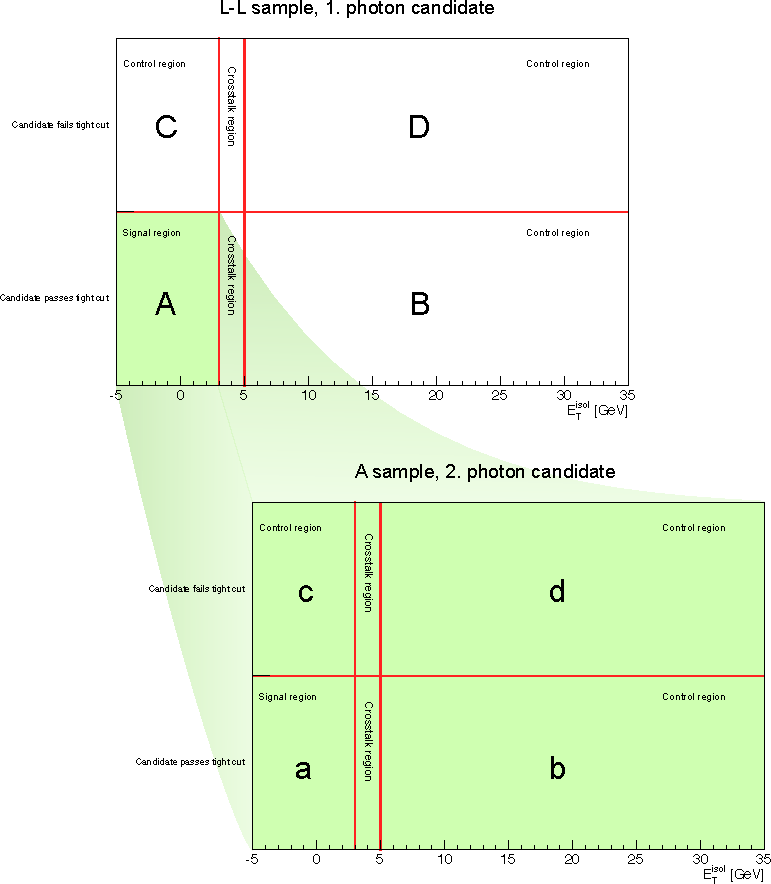
\includegraphics[width=\textwidth]{figures/sideband}
  \caption{Illustrating the two--step ABCD method, adapted from \cite{fdirect} using the `tight' selection criteria and the isolation energy: the full set of diphotons (the L-L sample) is split into four groups---A, B, C and D---according to the discriminating variables for the leading photon. Signal photons are now confined to the A region. The events in the C region can be used to estimate the shape, and the B and D region can be used to estimate the magnitude of the distribution of background events in the signal region. The procedure is then repeated for the subleading partner photons of the events in the A region. This gives an estimate of the distribution of background events in the combined signal (Aa) region.}\label{abcd}
\end{figure}

This is also known as the two--dimensional sideband method \cite{cmsabcd}. The following description may be aided by the illustration in figure~\ref{abcd}.

To reiterate, we need to examine our sample of signal and background data points in terms of two uncorrelated discriminating variables, call them $x$ and $y$. With this, we can split the data set into four regions:

\begin{itemize}
\item[{\bfseries\sffamily\color{natgreen}A:}] The signal region in both discriminating variables. This region should contain all signal events.
\item[{\bfseries\sffamily\color{natgreen}B:}] The signal region in the $y$ variable, but not in $x$. We assume that the distribution of background events in $y$ in this regions will have the same shape as the distribution of background events in $y$ in the signal region, A.
\item[{\bfseries\sffamily\color{natgreen}C:}] As above, but with $x$ and $y$ exchanged.
\item[{\bfseries\sffamily\color{natgreen}D:}] The control region for both variables. Once again, we assume that the distribution of background events has the same shape for either variable in the control region as it has in its signal region. We expect the distribution in $x$ to have the same shape in the D region as it does in the B region, for example.
\end{itemize}

Thus, the distribution in $x$ of background events in the A region, $A_{bck}$, is assumed to be the shape of the distribution of events in the C region, scaled so that the distribution of events in $x$ in the B and D regions have the same magnitude:
\(A_{bck}=C\frac BD.\label{abckfind}\)
The signal distribution must then be given as
\(A_{sig}=A-A_{bck}.\label{asig}\)

As we are working with events with two photons, both of which give rise to independent backgrounds, this procedure must be repeated for the subleading photons as well. For the subleading photon candidate, we look at the sample of photon candidates that are the subleading partner of a selected photon in the signal, A, region of the distribution of leading photon candidates. Carrying out the ABCD procedure on the sample of subleading photons gives us $Aa_{bck}$, an estimate of the number of selected photon pairs where the leading photon is in the A region and the subleading photon is a part of the background in the Aa region.
Using \eqref{asig}, we can now write the number of events in the signal--signal region as
\(\begin{aligned}
A_{sig}a_{sig} &=(A-A_{bck})a-(A-A_{bck})a_{bck}\\ &=Aa-A_{bck}a-Aa_{bck}+A_{bck}a_{bck}\\&=Aa-[Aa]_{bck}.
\end{aligned}\)
$Aa$ is the number of events in the Aa region, which is readily available. Of the terms that contribute to the total background $[Aa]_{bkc}$, $Aa_{bck}$, the total number of background subleading photons in the Aa region, is determined by taking
\(Aa_{bck}=Ac\frac{Ab}{Ad},\)
analogous to how $A_{bck}$ sample was found in eq.~\eqref{abckfind}. We find $A_{bck}A$, the total number background leading photons in the Aa region, and $A_{bck}a_{bck}$, the number of photon pairs in the Aa region where both members are background photons, by multiplying $Aa$ and $Aa_{bck}$ by
\(f_{bck}=\frac{A_{bck}}{A},\)
the fraction of background events in the leading photon A sample. Thus, the total estimated background in the AA region is given by
\([Aa]_{bck}=\frac{A_{bck}}{A}(Aa)+Aa_{bck}-\frac{A_{bck}}{A}(Aa_{bck}),\)
which we can interpret as the number of data points where the leading photon was a background plus the number of data points where the subleading photon was a background, subtracted the number of data points where both photons were background events, which would have been double counted.

For the diphoton sample, the choice of the two discriminants are the `tight' selection criteria, which were described in chapter~\ref{ch.exp}, and the transverse isolation energy, $E_T^{\text{isol}}$, the energy deposited in the calorimeter in a cone with radius $R\le0.4$, but outside $R\le0.2$, where
\[R=\sqrt{\Delta\phi^2+\Delta\theta^2}.\]
The signal region is defined as $E_T^{\text{isol}}\le3$ GeV. Allowing a crosstalk region of 2 GeV, which means the background region is $5\text{ GeV}\le E_T^{\text{isol}}\le25\text{ GeV}$, produces the distribution of $E_T^{\text{isol}}$ for leading photons and subleading photons in the `A' sample is given in figure~\ref{etiso}. As the figure shows, the tight and loose selections are identical in the background region, whereas they diverge in the crosstalk region, which is the desired behaviour.

\begin{figure}[htp]
\begin{minipage}[b]{.69\textwidth}
\begin{infilsf} \tiny 
\begin{tikzpicture}[x=.1\textwidth,y=.1\textwidth]
\pgfdeclareplotmark{cross} {
\pgfpathmoveto{\pgfpoint{-0.3\pgfplotmarksize}{\pgfplotmarksize}}
\pgfpathlineto{\pgfpoint{+0.3\pgfplotmarksize}{\pgfplotmarksize}}
\pgfpathlineto{\pgfpoint{+0.3\pgfplotmarksize}{0.3\pgfplotmarksize}}
\pgfpathlineto{\pgfpoint{+1\pgfplotmarksize}{0.3\pgfplotmarksize}}
\pgfpathlineto{\pgfpoint{+1\pgfplotmarksize}{-0.3\pgfplotmarksize}}
\pgfpathlineto{\pgfpoint{+0.3\pgfplotmarksize}{-0.3\pgfplotmarksize}}
\pgfpathlineto{\pgfpoint{+0.3\pgfplotmarksize}{-1.\pgfplotmarksize}}
\pgfpathlineto{\pgfpoint{-0.3\pgfplotmarksize}{-1.\pgfplotmarksize}}
\pgfpathlineto{\pgfpoint{-0.3\pgfplotmarksize}{-0.3\pgfplotmarksize}}
\pgfpathlineto{\pgfpoint{-1.\pgfplotmarksize}{-0.3\pgfplotmarksize}}
\pgfpathlineto{\pgfpoint{-1.\pgfplotmarksize}{0.3\pgfplotmarksize}}
\pgfpathlineto{\pgfpoint{-0.3\pgfplotmarksize}{0.3\pgfplotmarksize}}
\pgfpathclose
\pgfusepathqstroke
}
\pgfdeclareplotmark{cross*} {
\pgfpathmoveto{\pgfpoint{-0.3\pgfplotmarksize}{\pgfplotmarksize}}
\pgfpathlineto{\pgfpoint{+0.3\pgfplotmarksize}{\pgfplotmarksize}}
\pgfpathlineto{\pgfpoint{+0.3\pgfplotmarksize}{0.3\pgfplotmarksize}}
\pgfpathlineto{\pgfpoint{+1\pgfplotmarksize}{0.3\pgfplotmarksize}}
\pgfpathlineto{\pgfpoint{+1\pgfplotmarksize}{-0.3\pgfplotmarksize}}
\pgfpathlineto{\pgfpoint{+0.3\pgfplotmarksize}{-0.3\pgfplotmarksize}}
\pgfpathlineto{\pgfpoint{+0.3\pgfplotmarksize}{-1.\pgfplotmarksize}}
\pgfpathlineto{\pgfpoint{-0.3\pgfplotmarksize}{-1.\pgfplotmarksize}}
\pgfpathlineto{\pgfpoint{-0.3\pgfplotmarksize}{-0.3\pgfplotmarksize}}
\pgfpathlineto{\pgfpoint{-1.\pgfplotmarksize}{-0.3\pgfplotmarksize}}
\pgfpathlineto{\pgfpoint{-1.\pgfplotmarksize}{0.3\pgfplotmarksize}}
\pgfpathlineto{\pgfpoint{-0.3\pgfplotmarksize}{0.3\pgfplotmarksize}}
\pgfpathclose
\pgfusepathqfillstroke
}
\pgfdeclareplotmark{newstar} {
\pgfpathmoveto{\pgfqpoint{0pt}{\pgfplotmarksize}}
\pgfpathlineto{\pgfqpointpolar{44}{0.5\pgfplotmarksize}}
\pgfpathlineto{\pgfqpointpolar{18}{\pgfplotmarksize}}
\pgfpathlineto{\pgfqpointpolar{-20}{0.5\pgfplotmarksize}}
\pgfpathlineto{\pgfqpointpolar{-54}{\pgfplotmarksize}}
\pgfpathlineto{\pgfqpointpolar{-90}{0.5\pgfplotmarksize}}
\pgfpathlineto{\pgfqpointpolar{234}{\pgfplotmarksize}}
\pgfpathlineto{\pgfqpointpolar{198}{0.5\pgfplotmarksize}}
\pgfpathlineto{\pgfqpointpolar{162}{\pgfplotmarksize}}
\pgfpathlineto{\pgfqpointpolar{134}{0.5\pgfplotmarksize}}
\pgfpathclose
\pgfusepathqstroke
}
\pgfdeclareplotmark{newstar*} {
\pgfpathmoveto{\pgfqpoint{0pt}{\pgfplotmarksize}}
\pgfpathlineto{\pgfqpointpolar{44}{0.5\pgfplotmarksize}}
\pgfpathlineto{\pgfqpointpolar{18}{\pgfplotmarksize}}
\pgfpathlineto{\pgfqpointpolar{-20}{0.5\pgfplotmarksize}}
\pgfpathlineto{\pgfqpointpolar{-54}{\pgfplotmarksize}}
\pgfpathlineto{\pgfqpointpolar{-90}{0.5\pgfplotmarksize}}
\pgfpathlineto{\pgfqpointpolar{234}{\pgfplotmarksize}}
\pgfpathlineto{\pgfqpointpolar{198}{0.5\pgfplotmarksize}}
\pgfpathlineto{\pgfqpointpolar{162}{\pgfplotmarksize}}
\pgfpathlineto{\pgfqpointpolar{134}{0.5\pgfplotmarksize}}
\pgfpathclose
\pgfusepathqfillstroke
}
\definecolor{c}{rgb}{1,1,1};
\draw [color=c, fill=c] (1,0.679598) rectangle (9,6.11638);
\definecolor{c}{rgb}{0,0,0};
\draw [c] (1,0.679598) -- (1,6.11638) -- (9,6.11638) -- (9,0.679598) -- (1,0.679598);
\definecolor{c}{rgb}{1,1,1};
\draw [color=c, fill=c] (1,0.679598) rectangle (9,6.11638);
\definecolor{c}{rgb}{0,0,0};
\draw [c] (1,0.679598) -- (1,6.11638) -- (9,6.11638) -- (9,0.679598) -- (1,0.679598);
\colorlet{c}{natgreen}
\draw [c] (1,0.680318) -- (1.0293,0.680318) -- (1.0293,0.681757) -- (1.05861,0.681757) -- (1.05861,0.681757) -- (1.08791,0.681757) -- (1.08791,0.683197) -- (1.11722,0.683197) -- (1.11722,0.682837) -- (1.14652,0.682837) -- (1.14652,0.682837) --
 (1.17582,0.682837) -- (1.17582,0.684637) -- (1.20513,0.684637) -- (1.20513,0.686437) -- (1.23443,0.686437) -- (1.23443,0.689676) -- (1.26374,0.689676) -- (1.26374,0.691476) -- (1.29304,0.691476) -- (1.29304,0.692916) -- (1.32234,0.692916) --
 (1.32234,0.700115) -- (1.35165,0.700115) -- (1.35165,0.706594) -- (1.38095,0.706594) -- (1.38095,0.718832) -- (1.41026,0.718832) -- (1.41026,0.730711) -- (1.43956,0.730711) -- (1.43956,0.73251) -- (1.46886,0.73251) -- (1.46886,0.749428) --
 (1.49817,0.749428) -- (1.49817,0.765986) -- (1.52747,0.765986) -- (1.52747,0.803421) -- (1.55678,0.803421) -- (1.55678,0.825378) -- (1.58608,0.825378) -- (1.58608,0.872891) -- (1.61538,0.872891) -- (1.61538,0.916085) -- (1.64469,0.916085) --
 (1.64469,0.980156) -- (1.67399,0.980156) -- (1.67399,1.02983) -- (1.7033,1.02983) -- (1.7033,1.13098) -- (1.7326,1.13098) -- (1.7326,1.24976) -- (1.7619,1.24976) -- (1.7619,1.36998) -- (1.79121,1.36998) -- (1.79121,1.47797) -- (1.82051,1.47797) --
 (1.82051,1.70258) -- (1.84982,1.70258) -- (1.84982,1.88471) -- (1.87912,1.88471) -- (1.87912,2.13668) -- (1.90842,2.13668) -- (1.90842,2.44264) -- (1.93773,2.44264) -- (1.93773,2.74931) -- (1.96703,2.74931) -- (1.96703,3.11538) -- (1.99634,3.11538)
 -- (1.99634,3.51025) -- (2.02564,3.51025) -- (2.02564,3.91339) -- (2.05494,3.91339) -- (2.05494,4.39969) -- (2.08425,4.39969) -- (2.08425,4.83019) -- (2.11355,4.83019) -- (2.11355,5.25133) -- (2.14286,5.25133) -- (2.14286,5.5742) -- (2.17216,5.5742)
 -- (2.17216,5.74302) -- (2.20147,5.74302) -- (2.20147,5.85748) -- (2.23077,5.85748) -- (2.23077,5.71314) -- (2.26007,5.71314) -- (2.26007,5.43346) -- (2.28938,5.43346) -- (2.28938,5.30064) -- (2.31868,5.30064) -- (2.31868,5.13362) --
 (2.34799,5.13362) -- (2.34799,4.86654) -- (2.37729,4.86654) -- (2.37729,4.65165) -- (2.40659,4.65165) -- (2.40659,4.41552) -- (2.4359,4.41552) -- (2.4359,4.16608) -- (2.4652,4.16608) -- (2.4652,4.03974) -- (2.49451,4.03974) -- (2.49451,3.90655) --
 (2.52381,3.90655) -- (2.52381,3.68158) -- (2.55311,3.68158) -- (2.55311,3.57216) -- (2.58242,3.57216) -- (2.58242,3.35511) -- (2.61172,3.35511) -- (2.61172,3.31767) -- (2.64103,3.31767) -- (2.64103,3.12546) -- (2.67033,3.12546) -- (2.67033,2.98292)
 -- (2.69963,2.98292) -- (2.69963,2.8429) -- (2.72894,2.8429) -- (2.72894,2.79683) -- (2.75824,2.79683) -- (2.75824,2.59309) -- (2.78755,2.59309) -- (2.78755,2.60389) -- (2.81685,2.60389) -- (2.81685,2.42572) -- (2.84615,2.42572) -- (2.84615,2.37208)
 -- (2.87546,2.37208) -- (2.87546,2.2821) -- (2.90476,2.2821) -- (2.90476,2.19823) -- (2.93407,2.19823) -- (2.93407,2.105) -- (2.96337,2.105) -- (2.96337,2.07477) -- (2.99267,2.07477) -- (2.99267,1.9513) -- (3.02198,1.9513) -- (3.02198,1.91567) --
 (3.05128,1.91567) -- (3.05128,1.8552) -- (3.08059,1.8552) -- (3.08059,1.80192) -- (3.10989,1.80192) -- (3.10989,1.72813) -- (3.13919,1.72813) -- (3.13919,1.70582) -- (3.1685,1.70582) -- (3.1685,1.66298) -- (3.1978,1.66298) -- (3.1978,1.60575) --
 (3.22711,1.60575) -- (3.22711,1.58127) -- (3.25641,1.58127) -- (3.25641,1.53772) -- (3.28571,1.53772) -- (3.28571,1.48373) -- (3.31502,1.48373) -- (3.31502,1.43441) -- (3.34432,1.43441) -- (3.34432,1.44557) -- (3.37363,1.44557) -- (3.37363,1.37754)
 -- (3.40293,1.37754) -- (3.40293,1.35594) -- (3.43223,1.35594) -- (3.43223,1.32931) -- (3.46154,1.32931) -- (3.46154,1.29151) -- (3.49084,1.29151) -- (3.49084,1.30159) -- (3.52015,1.30159) -- (3.52015,1.23608) -- (3.54945,1.23608) --
 (3.54945,1.2476) -- (3.57875,1.2476) -- (3.57875,1.20405) -- (3.60806,1.20405) -- (3.60806,1.19361) -- (3.63736,1.19361) -- (3.63736,1.19181) -- (3.66667,1.19181) -- (3.66667,1.18497) -- (3.69597,1.18497) -- (3.69597,1.14357) -- (3.72527,1.14357) --
 (3.72527,1.11766) -- (3.75458,1.11766) -- (3.75458,1.10074) -- (3.78388,1.10074) -- (3.78388,1.0705) -- (3.81319,1.0705) -- (3.81319,1.08454) -- (3.84249,1.08454) -- (3.84249,1.04675) -- (3.87179,1.04675) -- (3.87179,1.03523) -- (3.9011,1.03523) --
 (3.9011,1.01651) -- (3.9304,1.01651) -- (3.9304,1.01939) -- (3.95971,1.01939) -- (3.95971,1.01039) -- (3.98901,1.01039) -- (3.98901,1.01363) -- (4.01831,1.01363) -- (4.01831,0.979796) -- (4.04762,0.979796) -- (4.04762,0.969358) -- (4.07692,0.969358)
 -- (4.07692,0.944881) -- (4.10623,0.944881) -- (4.10623,0.95316) -- (4.13553,0.95316) -- (4.13553,0.927604) -- (4.16483,0.927604) -- (4.16483,0.927244) -- (4.19414,0.927244) -- (4.19414,0.899168) -- (4.22344,0.899168) -- (4.22344,0.907446) --
 (4.25275,0.907446) -- (4.25275,0.914285) -- (4.28205,0.914285) -- (4.28205,0.890529) -- (4.31136,0.890529) -- (4.31136,0.901687) -- (4.34066,0.901687) -- (4.34066,0.898088) -- (4.36996,0.898088) -- (4.36996,0.88369) -- (4.39927,0.88369) --
 (4.39927,0.87793) -- (4.42857,0.87793) -- (4.42857,0.867852) -- (4.45788,0.867852) -- (4.45788,0.859573) -- (4.48718,0.859573) -- (4.48718,0.850574) -- (4.51648,0.850574) -- (4.51648,0.849854) -- (4.54579,0.849854) -- (4.54579,0.854174) --
 (4.57509,0.854174) -- (4.57509,0.852014) -- (4.6044,0.852014) -- (4.6044,0.847695) -- (4.6337,0.847695) -- (4.6337,0.823578) -- (4.663,0.823578) -- (4.663,0.833297) -- (4.69231,0.833297) -- (4.69231,0.818539) -- (4.72161,0.818539) --
 (4.72161,0.802701) -- (4.75092,0.802701) -- (4.75092,0.818539) -- (4.78022,0.818539) -- (4.78022,0.813499) -- (4.80952,0.813499) -- (4.80952,0.81134) -- (4.83883,0.81134) -- (4.83883,0.799101) -- (4.86813,0.799101) -- (4.86813,0.789743) --
 (4.89744,0.789743) -- (4.89744,0.796942) -- (4.92674,0.796942) -- (4.92674,0.792262) -- (4.95604,0.792262) -- (4.95604,0.795502) -- (4.98535,0.795502) -- (4.98535,0.797661) -- (5.01465,0.797661) -- (5.01465,0.777144) -- (5.04396,0.777144) --
 (5.04396,0.783983) -- (5.07326,0.783983) -- (5.07326,0.776784) -- (5.10256,0.776784) -- (5.10256,0.770305) -- (5.13187,0.770305) -- (5.13187,0.773545) -- (5.16117,0.773545) -- (5.16117,0.778584) -- (5.19048,0.778584) -- (5.19048,0.772465) --
 (5.21978,0.772465) -- (5.21978,0.764186) -- (5.24908,0.764186) -- (5.24908,0.763106) -- (5.27839,0.763106) -- (5.27839,0.760227) -- (5.30769,0.760227) -- (5.30769,0.762026) -- (5.337,0.762026) -- (5.337,0.756627) -- (5.3663,0.756627) --
 (5.3663,0.762746) -- (5.3956,0.762746) -- (5.3956,0.757707) -- (5.42491,0.757707) -- (5.42491,0.755187) -- (5.45421,0.755187) -- (5.45421,0.747628) -- (5.48352,0.747628) -- (5.48352,0.745469) -- (5.51282,0.745469) -- (5.51282,0.747268) --
 (5.54212,0.747268) -- (5.54212,0.753388) -- (5.57143,0.753388) -- (5.57143,0.746908) -- (5.60073,0.746908) -- (5.60073,0.73827) -- (5.63004,0.73827) -- (5.63004,0.741869) -- (5.65934,0.741869) -- (5.65934,0.742229) -- (5.68864,0.742229) --
 (5.68864,0.739709) -- (5.71795,0.739709) -- (5.71795,0.73863) -- (5.74725,0.73863) -- (5.74725,0.731431) -- (5.77656,0.731431) -- (5.77656,0.728551) -- (5.80586,0.728551) -- (5.80586,0.731431) -- (5.83517,0.731431) -- (5.83517,0.731791) --
 (5.86447,0.731791) -- (5.86447,0.730351) -- (5.89377,0.730351) -- (5.89377,0.725671) -- (5.92308,0.725671) -- (5.92308,0.73935) -- (5.95238,0.73935) -- (5.95238,0.731791) -- (5.98169,0.731791) -- (5.98169,0.727111) -- (6.01099,0.727111) --
 (6.01099,0.728551) -- (6.04029,0.728551) -- (6.04029,0.73467) -- (6.0696,0.73467) -- (6.0696,0.723152) -- (6.0989,0.723152) -- (6.0989,0.728191) -- (6.12821,0.728191) -- (6.12821,0.722792) -- (6.15751,0.722792) -- (6.15751,0.726391) --
 (6.18681,0.726391) -- (6.18681,0.720632) -- (6.21612,0.720632) -- (6.21612,0.717033) -- (6.24542,0.717033) -- (6.24542,0.722432) -- (6.27473,0.722432) -- (6.27473,0.715593) -- (6.30403,0.715593) -- (6.30403,0.719552) -- (6.33333,0.719552) --
 (6.33333,0.717753) -- (6.36264,0.717753) -- (6.36264,0.717393) -- (6.39194,0.717393) -- (6.39194,0.714153) -- (6.42125,0.714153) -- (6.42125,0.716673) -- (6.45055,0.716673) -- (6.45055,0.713433) -- (6.47985,0.713433) -- (6.47985,0.719192) --
 (6.50916,0.719192) -- (6.50916,0.712353) -- (6.53846,0.712353) -- (6.53846,0.713793) -- (6.56777,0.713793) -- (6.56777,0.715593) -- (6.59707,0.715593) -- (6.59707,0.710194) -- (6.62637,0.710194) -- (6.62637,0.718832) -- (6.65568,0.718832) --
 (6.65568,0.713793) -- (6.68498,0.713793) -- (6.68498,0.706954) -- (6.71429,0.706954) -- (6.71429,0.715593) -- (6.74359,0.715593) -- (6.74359,0.708394) -- (6.77289,0.708394) -- (6.77289,0.711633) -- (6.8022,0.711633) -- (6.8022,0.708394) --
 (6.8315,0.708394) -- (6.8315,0.705154) -- (6.86081,0.705154) -- (6.86081,0.707314) -- (6.89011,0.707314) -- (6.89011,0.711633) -- (6.91941,0.711633) -- (6.91941,0.709834) -- (6.94872,0.709834) -- (6.94872,0.707314) -- (6.97802,0.707314) --
 (6.97802,0.707314) -- (7.00733,0.707314) -- (7.00733,0.704434) -- (7.03663,0.704434) -- (7.03663,0.707314) -- (7.06593,0.707314) -- (7.06593,0.706954) -- (7.09524,0.706954) -- (7.09524,0.703354) -- (7.12454,0.703354) -- (7.12454,0.704794) --
 (7.15385,0.704794) -- (7.15385,0.708754) -- (7.18315,0.708754) -- (7.18315,0.703714) -- (7.21245,0.703714) -- (7.21245,0.709834) -- (7.24176,0.709834) -- (7.24176,0.699755) -- (7.27106,0.699755) -- (7.27106,0.702275) -- (7.30037,0.702275) --
 (7.30037,0.704074) -- (7.32967,0.704074) -- (7.32967,0.700835) -- (7.35897,0.700835) -- (7.35897,0.703354) -- (7.38828,0.703354) -- (7.38828,0.705514) -- (7.41758,0.705514) -- (7.41758,0.696155) -- (7.44689,0.696155) -- (7.44689,0.697595) --
 (7.47619,0.697595) -- (7.47619,0.708034) -- (7.50549,0.708034) -- (7.50549,0.700835) -- (7.5348,0.700835) -- (7.5348,0.700115) -- (7.5641,0.700115) -- (7.5641,0.698315) -- (7.59341,0.698315) -- (7.59341,0.697955) -- (7.62271,0.697955) --
 (7.62271,0.700835) -- (7.65201,0.700835) -- (7.65201,0.702635) -- (7.68132,0.702635) -- (7.68132,0.694716) -- (7.71062,0.694716) -- (7.71062,0.698315) -- (7.73993,0.698315) -- (7.73993,0.703354) -- (7.76923,0.703354) -- (7.76923,0.694716) --
 (7.79853,0.694716) -- (7.79853,0.699035) -- (7.82784,0.699035) -- (7.82784,0.697955) -- (7.85714,0.697955) -- (7.85714,0.697955) -- (7.88645,0.697955) -- (7.88645,0.699755) -- (7.91575,0.699755) -- (7.91575,0.701195) -- (7.94506,0.701195) --
 (7.94506,0.699755) -- (7.97436,0.699755) -- (7.97436,0.694356) -- (8.00366,0.694356) -- (8.00366,0.697955) -- (8.03297,0.697955) -- (8.03297,0.696515) -- (8.06227,0.696515) -- (8.06227,0.697595) -- (8.09157,0.697595) -- (8.09157,0.694356) --
 (8.12088,0.694356) -- (8.12088,0.699395) -- (8.15018,0.699395) -- (8.15018,0.695076) -- (8.17949,0.695076) -- (8.17949,0.695796) -- (8.20879,0.695796) -- (8.20879,0.695436) -- (8.2381,0.695436) -- (8.2381,0.697235) -- (8.2674,0.697235) --
 (8.2674,0.694716) -- (8.2967,0.694716) -- (8.2967,0.694356) -- (8.32601,0.694356) -- (8.32601,0.692556) -- (8.35531,0.692556) -- (8.35531,0.692196) -- (8.38461,0.692196) -- (8.38461,0.695076) -- (8.41392,0.695076) -- (8.41392,0.697235) --
 (8.44322,0.697235) -- (8.44322,0.694716) -- (8.47253,0.694716) -- (8.47253,0.696155) -- (8.50183,0.696155) -- (8.50183,0.694716) -- (8.53114,0.694716) -- (8.53114,0.696155) -- (8.56044,0.696155) -- (8.56044,0.692916) -- (8.58974,0.692916) --
 (8.58974,0.693276) -- (8.61905,0.693276) -- (8.61905,0.688596) -- (8.64835,0.688596) -- (8.64835,0.691476) -- (8.67766,0.691476) -- (8.67766,0.690756) -- (8.70696,0.690756) -- (8.70696,0.688956) -- (8.73626,0.688956) -- (8.73626,0.691476) --
 (8.76557,0.691476) -- (8.76557,0.691476) -- (8.79487,0.691476) -- (8.79487,0.695796) -- (8.82418,0.695796) -- (8.82418,0.692556) -- (8.85348,0.692556) -- (8.85348,0.692556) -- (8.88278,0.692556) -- (8.88278,0.693996) -- (8.91209,0.693996) --
 (8.91209,0.695076) -- (8.94139,0.695076) -- (8.94139,0.689676) -- (8.9707,0.689676) -- (8.9707,0.691116) -- (9,0.691116);
\definecolor{c}{rgb}{0,0,0};
\draw [c] (1,0.679598) -- (9,0.679598);
\draw [anchor= east] (9,0.299023) node[color=c, rotate=0]{$E_{T}^{\text{isol}}$ [GeV]};
\draw [c] (1,0.842701) -- (1,0.679598);
\draw [c] (1.2664,0.761149) -- (1.2664,0.679598);
\draw [c] (1.5328,0.761149) -- (1.5328,0.679598);
\draw [c] (1.7992,0.761149) -- (1.7992,0.679598);
\draw [c] (2.0656,0.761149) -- (2.0656,0.679598);
\draw [c] (2.332,0.842701) -- (2.332,0.679598);
\draw [c] (2.5984,0.761149) -- (2.5984,0.679598);
\draw [c] (2.8648,0.761149) -- (2.8648,0.679598);
\draw [c] (3.1312,0.761149) -- (3.1312,0.679598);
\draw [c] (3.3976,0.761149) -- (3.3976,0.679598);
\draw [c] (3.664,0.842701) -- (3.664,0.679598);
\draw [c] (3.9304,0.761149) -- (3.9304,0.679598);
\draw [c] (4.1968,0.761149) -- (4.1968,0.679598);
\draw [c] (4.4632,0.761149) -- (4.4632,0.679598);
\draw [c] (4.7296,0.761149) -- (4.7296,0.679598);
\draw [c] (4.996,0.842701) -- (4.996,0.679598);
\draw [c] (5.2624,0.761149) -- (5.2624,0.679598);
\draw [c] (5.5288,0.761149) -- (5.5288,0.679598);
\draw [c] (5.7952,0.761149) -- (5.7952,0.679598);
\draw [c] (6.0616,0.761149) -- (6.0616,0.679598);
\draw [c] (6.32801,0.842701) -- (6.32801,0.679598);
\draw [c] (6.59441,0.761149) -- (6.59441,0.679598);
\draw [c] (6.86081,0.761149) -- (6.86081,0.679598);
\draw [c] (7.12721,0.761149) -- (7.12721,0.679598);
\draw [c] (7.39361,0.761149) -- (7.39361,0.679598);
\draw [c] (7.66001,0.842701) -- (7.66001,0.679598);
\draw [c] (7.92641,0.761149) -- (7.92641,0.679598);
\draw [c] (8.19281,0.761149) -- (8.19281,0.679598);
\draw [c] (8.45921,0.761149) -- (8.45921,0.679598);
\draw [c] (8.72561,0.761149) -- (8.72561,0.679598);
\draw [c] (8.99201,0.842701) -- (8.99201,0.679598);
\draw [c] (8.99201,0.842701) -- (8.99201,0.679598);
\draw [anchor=base] (1,0.455331) node[color=c, rotate=0]{-5};
\draw [anchor=base] (2.332,0.455331) node[color=c, rotate=0]{0};
\draw [anchor=base] (3.664,0.455331) node[color=c, rotate=0]{5};
\draw [anchor=base] (4.996,0.455331) node[color=c, rotate=0]{10};
\draw [anchor=base] (6.32801,0.455331) node[color=c, rotate=0]{15};
\draw [anchor=base] (7.66001,0.455331) node[color=c, rotate=0]{20};
\draw [anchor=base] (8.99201,0.455331) node[color=c, rotate=0]{25};
\draw [c] (1,0.679598) -- (1,6.11638);
\draw [anchor= east] (0.0,6.11638) node[color=c, rotate=90]{Number of events};
\draw [c] (1.24,0.679598) -- (1,0.679598);
\draw [c] (1.12,0.859573) -- (1,0.859573);
\draw [c] (1.12,1.03955) -- (1,1.03955);
\draw [c] (1.12,1.21952) -- (1,1.21952);
\draw [c] (1.24,1.3995) -- (1,1.3995);
\draw [c] (1.12,1.57947) -- (1,1.57947);
\draw [c] (1.12,1.75945) -- (1,1.75945);
\draw [c] (1.12,1.93942) -- (1,1.93942);
\draw [c] (1.24,2.1194) -- (1,2.1194);
\draw [c] (1.12,2.29937) -- (1,2.29937);
\draw [c] (1.12,2.47935) -- (1,2.47935);
\draw [c] (1.12,2.65933) -- (1,2.65933);
\draw [c] (1.24,2.8393) -- (1,2.8393);
\draw [c] (1.12,3.01928) -- (1,3.01928);
\draw [c] (1.12,3.19925) -- (1,3.19925);
\draw [c] (1.12,3.37923) -- (1,3.37923);
\draw [c] (1.24,3.5592) -- (1,3.5592);
\draw [c] (1.12,3.73918) -- (1,3.73918);
\draw [c] (1.12,3.91915) -- (1,3.91915);
\draw [c] (1.12,4.09913) -- (1,4.09913);
\draw [c] (1.24,4.2791) -- (1,4.2791);
\draw [c] (1.12,4.45908) -- (1,4.45908);
\draw [c] (1.12,4.63905) -- (1,4.63905);
\draw [c] (1.12,4.81903) -- (1,4.81903);
\draw [c] (1.24,4.999) -- (1,4.999);
\draw [c] (1.12,5.17898) -- (1,5.17898);
\draw [c] (1.12,5.35895) -- (1,5.35895);
\draw [c] (1.12,5.53893) -- (1,5.53893);
\draw [c] (1.24,5.7189) -- (1,5.7189);
\draw [c] (1.24,5.7189) -- (1,5.7189);
\draw [c] (1.12,5.89888) -- (1,5.89888);
\draw [c] (1.12,6.07885) -- (1,6.07885);
\draw [anchor= east] (0.95,0.679598) node[color=c, rotate=0]{0};
\draw [anchor= east] (0.95,1.3995) node[color=c, rotate=0]{2000};
\draw [anchor= east] (0.95,2.1194) node[color=c, rotate=0]{4000};
\draw [anchor= east] (0.95,2.8393) node[color=c, rotate=0]{6000};
\draw [anchor= east] (0.95,3.5592) node[color=c, rotate=0]{8000};
\draw [anchor= east] (0.95,4.2791) node[color=c, rotate=0]{10000};
\draw [anchor= east] (0.95,4.999) node[color=c, rotate=0]{12000};
\draw [anchor= east] (0.95,5.7189) node[color=c, rotate=0]{14000};
\colorlet{c}{natgreen!50}
\draw [c] (1,0.679598) -- (1.0293,0.679598) -- (1.0293,0.679598) -- (1.05861,0.679598) -- (1.05861,0.679598) -- (1.08791,0.679598) -- (1.08791,0.679598) -- (1.11722,0.679598) -- (1.11722,0.679598) -- (1.14652,0.679598) -- (1.14652,0.679598) --
 (1.17582,0.679598) -- (1.17582,0.679598) -- (1.20513,0.679598) -- (1.20513,0.680546) -- (1.23443,0.680546) -- (1.23443,0.680546) -- (1.26374,0.680546) -- (1.26374,0.681359) -- (1.29304,0.681359) -- (1.29304,0.682307) -- (1.32234,0.682307) --
 (1.32234,0.683526) -- (1.35165,0.683526) -- (1.35165,0.684745) -- (1.38095,0.684745) -- (1.38095,0.683932) -- (1.41026,0.683932) -- (1.41026,0.684339) -- (1.43956,0.684339) -- (1.43956,0.688267) -- (1.46886,0.688267) -- (1.46886,0.688809) --
 (1.49817,0.688809) -- (1.49817,0.694227) -- (1.52747,0.694227) -- (1.52747,0.694633) -- (1.55678,0.694633) -- (1.55678,0.700457) -- (1.58608,0.700457) -- (1.58608,0.707366) -- (1.61538,0.707366) -- (1.61538,0.715899) -- (1.64469,0.715899) --
 (1.64469,0.72362) -- (1.67399,0.72362) -- (1.67399,0.733643) -- (1.7033,0.733643) -- (1.7033,0.745834) -- (1.7326,0.745834) -- (1.7326,0.760327) -- (1.7619,0.760327) -- (1.7619,0.777665) -- (1.79121,0.777665) -- (1.79121,0.800963) --
 (1.82051,0.800963) -- (1.82051,0.835368) -- (1.84982,0.835368) -- (1.84982,0.859885) -- (1.87912,0.859885) -- (1.87912,0.894425) -- (1.90842,0.894425) -- (1.90842,0.9333) -- (1.93773,0.9333) -- (1.93773,0.997098) -- (1.96703,0.997098) --
 (1.96703,1.04207) -- (1.99634,1.04207) -- (1.99634,1.10776) -- (2.02564,1.10776) -- (2.02564,1.17413) -- (2.05494,1.17413) -- (2.05494,1.23211) -- (2.08425,1.23211) -- (2.08425,1.31907) -- (2.11355,1.31907) -- (2.11355,1.41091) -- (2.14286,1.41091)
 -- (2.14286,1.46563) -- (2.17216,1.46563) -- (2.17216,1.54798) -- (2.20147,1.54798) -- (2.20147,1.60487) -- (2.23077,1.60487) -- (2.23077,1.64267) -- (2.26007,1.64267) -- (2.26007,1.69346) -- (2.28938,1.69346) -- (2.28938,1.7471) -- (2.31868,1.7471)
 -- (2.31868,1.76268) -- (2.34799,1.76268) -- (2.34799,1.76769) -- (2.37729,1.76769) -- (2.37729,1.81401) -- (2.40659,1.81401) -- (2.40659,1.84151) -- (2.4359,1.84151) -- (2.4359,1.82675) -- (2.4652,1.82675) -- (2.4652,1.85478) -- (2.49451,1.85478)
 -- (2.49451,1.8407) -- (2.52381,1.8407) -- (2.52381,1.83988) -- (2.55311,1.83988) -- (2.55311,1.82796) -- (2.58242,1.82796) -- (2.58242,1.85668) -- (2.61172,1.85668) -- (2.61172,1.84584) -- (2.64103,1.84584) -- (2.64103,1.82295) -- (2.67033,1.82295)
 -- (2.67033,1.79099) -- (2.69963,1.79099) -- (2.69963,1.79884) -- (2.72894,1.79884) -- (2.72894,1.78286) -- (2.75824,1.78286) -- (2.75824,1.75401) -- (2.78755,1.75401) -- (2.78755,1.75645) -- (2.81685,1.75645) -- (2.81685,1.73829) --
 (2.84615,1.73829) -- (2.84615,1.70877) -- (2.87546,1.70877) -- (2.87546,1.67368) -- (2.90476,1.67368) -- (2.90476,1.6745) -- (2.93407,1.6745) -- (2.93407,1.65161) -- (2.96337,1.65161) -- (2.96337,1.62763) -- (2.99267,1.62763) -- (2.99267,1.60691) --
 (3.02198,1.60691) -- (3.02198,1.59566) -- (3.05128,1.59566) -- (3.05128,1.55841) -- (3.08059,1.55841) -- (3.08059,1.53782) -- (3.10989,1.53782) -- (3.10989,1.51981) -- (3.13919,1.51981) -- (3.13919,1.47863) -- (3.1685,1.47863) -- (3.1685,1.47863) --
 (3.1978,1.47863) -- (3.1978,1.45764) -- (3.22711,1.45764) -- (3.22711,1.43163) -- (3.25641,1.43163) -- (3.25641,1.40197) -- (3.28571,1.40197) -- (3.28571,1.38693) -- (3.31502,1.38693) -- (3.31502,1.36648) -- (3.34432,1.36648) -- (3.34432,1.33844) --
 (3.37363,1.33844) -- (3.37363,1.32665) -- (3.40293,1.32665) -- (3.40293,1.30078) -- (3.43223,1.30078) -- (3.43223,1.28575) -- (3.46154,1.28575) -- (3.46154,1.27545) -- (3.49084,1.27545) -- (3.49084,1.22601) -- (3.52015,1.22601) -- (3.52015,1.22452)
 -- (3.54945,1.22452) -- (3.54945,1.21003) -- (3.57875,1.21003) -- (3.57875,1.19256) -- (3.60806,1.19256) -- (3.60806,1.18158) -- (3.63736,1.18158) -- (3.63736,1.14285) -- (3.66667,1.14285) -- (3.66667,1.14027) -- (3.69597,1.14027) --
 (3.69597,1.13011) -- (3.72527,1.13011) -- (3.72527,1.11819) -- (3.75458,1.11819) -- (3.75458,1.08243) -- (3.78388,1.08243) -- (3.78388,1.08487) -- (3.81319,1.08487) -- (3.81319,1.07525) -- (3.84249,1.07525) -- (3.84249,1.06225) -- (3.87179,1.06225)
 -- (3.87179,1.05914) -- (3.9011,1.05914) -- (3.9011,1.0315) -- (3.9304,1.0315) -- (3.9304,1.0376) -- (3.95971,1.0376) -- (3.95971,1.01985) -- (3.98901,1.01985) -- (3.98901,1.01037) -- (4.01831,1.01037) -- (4.01831,0.988565) -- (4.04762,0.988565) --
 (4.04762,0.991139) -- (4.07692,0.991139) -- (4.07692,0.977458) -- (4.10623,0.977458) -- (4.10623,0.954295) -- (4.13553,0.954295) -- (4.13553,0.941292) -- (4.16483,0.941292) -- (4.16483,0.93926) -- (4.19414,0.93926) -- (4.19414,0.940886) --
 (4.22344,0.940886) -- (4.22344,0.919078) -- (4.25275,0.919078) -- (4.25275,0.91068) -- (4.28205,0.91068) -- (4.28205,0.893613) -- (4.31136,0.893613) -- (4.31136,0.911763) -- (4.34066,0.911763) -- (4.34066,0.899031) -- (4.36996,0.899031) --
 (4.36996,0.890633) -- (4.39927,0.890633) -- (4.39927,0.878713) -- (4.42857,0.878713) -- (4.42857,0.881016) -- (4.45788,0.881016) -- (4.45788,0.874243) -- (4.48718,0.874243) -- (4.48718,0.863949) -- (4.51648,0.863949) -- (4.51648,0.865845) --
 (4.54579,0.865845) -- (4.54579,0.850403) -- (4.57509,0.850403) -- (4.57509,0.845933) -- (4.6044,0.845933) -- (4.6044,0.84187) -- (4.6337,0.84187) -- (4.6337,0.842683) -- (4.663,0.842683) -- (4.663,0.837671) -- (4.69231,0.837671) --
 (4.69231,0.831711) -- (4.72161,0.831711) -- (4.72161,0.827512) -- (4.75092,0.827512) -- (4.75092,0.813831) -- (4.78022,0.813831) -- (4.78022,0.819249) -- (4.80952,0.819249) -- (4.80952,0.805162) -- (4.83883,0.805162) -- (4.83883,0.810987) --
 (4.86813,0.810987) -- (4.86813,0.809497) -- (4.89744,0.809497) -- (4.89744,0.80462) -- (4.92674,0.80462) -- (4.92674,0.801776) -- (4.95604,0.801776) -- (4.95604,0.794191) -- (4.98535,0.794191) -- (4.98535,0.80313) -- (5.01465,0.80313) --
 (5.01465,0.788231) -- (5.04396,0.788231) -- (5.04396,0.78051) -- (5.07326,0.78051) -- (5.07326,0.781458) -- (5.10256,0.781458) -- (5.10256,0.78349) -- (5.13187,0.78349) -- (5.13187,0.786741) -- (5.16117,0.786741) -- (5.16117,0.775634) --
 (5.19048,0.775634) -- (5.19048,0.775363) -- (5.21978,0.775363) -- (5.21978,0.770757) -- (5.24908,0.770757) -- (5.24908,0.76561) -- (5.27839,0.76561) -- (5.27839,0.761817) -- (5.30769,0.761817) -- (5.30769,0.766694) -- (5.337,0.766694) --
 (5.337,0.759108) -- (5.3663,0.759108) -- (5.3663,0.762359) -- (5.3956,0.762359) -- (5.3956,0.756535) -- (5.42491,0.756535) -- (5.42491,0.757889) -- (5.45421,0.757889) -- (5.45421,0.751929) -- (5.48352,0.751929) -- (5.48352,0.750846) --
 (5.51282,0.750846) -- (5.51282,0.754368) -- (5.54212,0.754368) -- (5.54212,0.747595) -- (5.57143,0.747595) -- (5.57143,0.742854) -- (5.60073,0.742854) -- (5.60073,0.746918) -- (5.63004,0.746918) -- (5.63004,0.744886) -- (5.65934,0.744886) --
 (5.65934,0.741906) -- (5.68864,0.741906) -- (5.68864,0.737301) -- (5.71795,0.737301) -- (5.71795,0.740281) -- (5.74725,0.740281) -- (5.74725,0.734591) -- (5.77656,0.734591) -- (5.77656,0.734727) -- (5.80586,0.734727) -- (5.80586,0.736352) --
 (5.83517,0.736352) -- (5.83517,0.733914) -- (5.86447,0.733914) -- (5.86447,0.734185) -- (5.89377,0.734185) -- (5.89377,0.726464) -- (5.92308,0.726464) -- (5.92308,0.732424) -- (5.95238,0.732424) -- (5.95238,0.730392) -- (5.98169,0.730392) --
 (5.98169,0.726871) -- (6.01099,0.726871) -- (6.01099,0.725516) -- (6.04029,0.725516) -- (6.04029,0.721588) -- (6.0696,0.721588) -- (6.0696,0.727277) -- (6.0989,0.727277) -- (6.0989,0.72362) -- (6.12821,0.72362) -- (6.12821,0.72064) --
 (6.15751,0.72064) -- (6.15751,0.720504) -- (6.18681,0.720504) -- (6.18681,0.721859) -- (6.21612,0.721859) -- (6.21612,0.720775) -- (6.24542,0.720775) -- (6.24542,0.718879) -- (6.27473,0.718879) -- (6.27473,0.715222) -- (6.30403,0.715222) --
 (6.30403,0.717389) -- (6.33333,0.717389) -- (6.33333,0.718473) -- (6.36264,0.718473) -- (6.36264,0.713732) -- (6.39194,0.713732) -- (6.39194,0.714544) -- (6.42125,0.714544) -- (6.42125,0.717931) -- (6.45055,0.717931) -- (6.45055,0.709939) --
 (6.47985,0.709939) -- (6.47985,0.711158) -- (6.50916,0.711158) -- (6.50916,0.715357) -- (6.53846,0.715357) -- (6.53846,0.714544) -- (6.56777,0.714544) -- (6.56777,0.712919) -- (6.59707,0.712919) -- (6.59707,0.711158) -- (6.62637,0.711158) --
 (6.62637,0.711835) -- (6.65568,0.711835) -- (6.65568,0.707095) -- (6.68498,0.707095) -- (6.68498,0.709397) -- (6.71429,0.709397) -- (6.71429,0.710481) -- (6.74359,0.710481) -- (6.74359,0.706146) -- (6.77289,0.706146) -- (6.77289,0.709939) --
 (6.8022,0.709939) -- (6.8022,0.706824) -- (6.8315,0.706824) -- (6.8315,0.707095) -- (6.86081,0.707095) -- (6.86081,0.703979) -- (6.89011,0.703979) -- (6.89011,0.70276) -- (6.91941,0.70276) -- (6.91941,0.703437) -- (6.94872,0.703437) --
 (6.94872,0.703708) -- (6.97802,0.703708) -- (6.97802,0.701541) -- (7.00733,0.701541) -- (7.00733,0.704656) -- (7.03663,0.704656) -- (7.03663,0.703031) -- (7.06593,0.703031) -- (7.06593,0.700999) -- (7.09524,0.700999) -- (7.09524,0.703979) --
 (7.12454,0.703979) -- (7.12454,0.700728) -- (7.15385,0.700728) -- (7.15385,0.700864) -- (7.18315,0.700864) -- (7.18315,0.702354) -- (7.21245,0.702354) -- (7.21245,0.701676) -- (7.24176,0.701676) -- (7.24176,0.699645) -- (7.27106,0.699645) --
 (7.27106,0.699238) -- (7.30037,0.699238) -- (7.30037,0.700051) -- (7.32967,0.700051) -- (7.32967,0.698426) -- (7.35897,0.698426) -- (7.35897,0.698697) -- (7.38828,0.698697) -- (7.38828,0.698019) -- (7.41758,0.698019) -- (7.41758,0.699103) --
 (7.44689,0.699103) -- (7.44689,0.697207) -- (7.47619,0.697207) -- (7.47619,0.695988) -- (7.50549,0.695988) -- (7.50549,0.696394) -- (7.5348,0.696394) -- (7.5348,0.693956) -- (7.5641,0.693956) -- (7.5641,0.696529) -- (7.59341,0.696529) --
 (7.59341,0.695852) -- (7.62271,0.695852) -- (7.62271,0.695988) -- (7.65201,0.695988) -- (7.65201,0.696123) -- (7.68132,0.696123) -- (7.68132,0.694633) -- (7.71062,0.694633) -- (7.71062,0.693956) -- (7.73993,0.693956) -- (7.73993,0.695717) --
 (7.76923,0.695717) -- (7.76923,0.69531) -- (7.79853,0.69531) -- (7.79853,0.692601) -- (7.82784,0.692601) -- (7.82784,0.693008) -- (7.85714,0.693008) -- (7.85714,0.694633) -- (7.88645,0.694633) -- (7.88645,0.693414) -- (7.91575,0.693414) --
 (7.91575,0.692601) -- (7.94506,0.692601) -- (7.94506,0.694768) -- (7.97436,0.694768) -- (7.97436,0.692601) -- (8.00366,0.692601) -- (8.00366,0.69233) -- (8.03297,0.69233) -- (8.03297,0.691924) -- (8.06227,0.691924) -- (8.06227,0.692466) --
 (8.09157,0.692466) -- (8.09157,0.69382) -- (8.12088,0.69382) -- (8.12088,0.691518) -- (8.15018,0.691518) -- (8.15018,0.694091) -- (8.17949,0.694091) -- (8.17949,0.69084) -- (8.20879,0.69084) -- (8.20879,0.691518) -- (8.2381,0.691518) --
 (8.2381,0.689215) -- (8.2674,0.689215) -- (8.2674,0.692737) -- (8.2967,0.692737) -- (8.2967,0.692737) -- (8.32601,0.692737) -- (8.32601,0.689892) -- (8.35531,0.689892) -- (8.35531,0.691382) -- (8.38461,0.691382) -- (8.38461,0.690163) --
 (8.41392,0.690163) -- (8.41392,0.69084) -- (8.44322,0.69084) -- (8.44322,0.689079) -- (8.47253,0.689079) -- (8.47253,0.69084) -- (8.50183,0.69084) -- (8.50183,0.690298) -- (8.53114,0.690298) -- (8.53114,0.690569) -- (8.56044,0.690569) --
 (8.56044,0.689757) -- (8.58974,0.689757) -- (8.58974,0.68786) -- (8.61905,0.68786) -- (8.61905,0.689215) -- (8.64835,0.689215) -- (8.64835,0.689079) -- (8.67766,0.689079) -- (8.67766,0.686912) -- (8.70696,0.686912) -- (8.70696,0.687319) --
 (8.73626,0.687319) -- (8.73626,0.688809) -- (8.76557,0.688809) -- (8.76557,0.68786) -- (8.79487,0.68786) -- (8.79487,0.68786) -- (8.82418,0.68786) -- (8.82418,0.688673) -- (8.85348,0.688673) -- (8.85348,0.687996) -- (8.88278,0.687996) --
 (8.88278,0.687319) -- (8.91209,0.687319) -- (8.91209,0.686912) -- (8.94139,0.686912) -- (8.94139,0.68786) -- (8.9707,0.68786) -- (8.9707,0.688538) -- (9,0.688538);
\colorlet{c}{natcomp}
\draw [c] (1,0.680318) -- (1.0293,0.680318) -- (1.0293,0.679598) -- (1.05861,0.679598) -- (1.05861,0.679598) -- (1.08791,0.679598) -- (1.08791,0.680318) -- (1.11722,0.680318) -- (1.11722,0.679598) -- (1.14652,0.679598) -- (1.14652,0.679598) --
 (1.17582,0.679598) -- (1.17582,0.680318) -- (1.20513,0.680318) -- (1.20513,0.682837) -- (1.23443,0.682837) -- (1.23443,0.680318) -- (1.26374,0.680318) -- (1.26374,0.683197) -- (1.29304,0.683197) -- (1.29304,0.681757) -- (1.32234,0.681757) --
 (1.32234,0.685717) -- (1.35165,0.685717) -- (1.35165,0.685357) -- (1.38095,0.685357) -- (1.38095,0.688956) -- (1.41026,0.688956) -- (1.41026,0.687877) -- (1.43956,0.687877) -- (1.43956,0.691836) -- (1.46886,0.691836) -- (1.46886,0.692196) --
 (1.49817,0.692196) -- (1.49817,0.700475) -- (1.52747,0.700475) -- (1.52747,0.708754) -- (1.55678,0.708754) -- (1.55678,0.710913) -- (1.58608,0.710913) -- (1.58608,0.717033) -- (1.61538,0.717033) -- (1.61538,0.73863) -- (1.64469,0.73863) --
 (1.64469,0.744389) -- (1.67399,0.744389) -- (1.67399,0.758787) -- (1.7033,0.758787) -- (1.7033,0.778584) -- (1.7326,0.778584) -- (1.7326,0.8117) -- (1.7619,0.8117) -- (1.7619,0.837256) -- (1.79121,0.837256) -- (1.79121,0.88117) -- (1.82051,0.88117)
 -- (1.82051,0.911046) -- (1.84982,0.911046) -- (1.84982,0.963959) -- (1.87912,0.963959) -- (1.87912,1.01687) -- (1.90842,1.01687) -- (1.90842,1.07518) -- (1.93773,1.07518) -- (1.93773,1.16121) -- (1.96703,1.16121) -- (1.96703,1.2476) --
 (1.99634,1.2476) -- (1.99634,1.34335) -- (2.02564,1.34335) -- (2.02564,1.41786) -- (2.05494,1.41786) -- (2.05494,1.57551) -- (2.08425,1.57551) -- (2.08425,1.66406) -- (2.11355,1.66406) -- (2.11355,1.78177) -- (2.14286,1.78177) -- (2.14286,1.83828)
 -- (2.17216,1.83828) -- (2.17216,1.90127) -- (2.20147,1.90127) -- (2.20147,1.94338) -- (2.23077,1.94338) -- (2.23077,1.90451) -- (2.26007,1.90451) -- (2.26007,1.88831) -- (2.28938,1.88831) -- (2.28938,1.848) -- (2.31868,1.848) -- (2.31868,1.78105)
 -- (2.34799,1.78105) -- (2.34799,1.73065) -- (2.37729,1.73065) -- (2.37729,1.71985) -- (2.40659,1.71985) -- (2.40659,1.6547) -- (2.4359,1.6547) -- (2.4359,1.58127) -- (2.4652,1.58127) -- (2.4652,1.55896) -- (2.49451,1.55896) -- (2.49451,1.49633) --
 (2.52381,1.49633) -- (2.52381,1.45529) -- (2.55311,1.45529) -- (2.55311,1.48049) -- (2.58242,1.48049) -- (2.58242,1.37682) -- (2.61172,1.37682) -- (2.61172,1.37862) -- (2.64103,1.37862) -- (2.64103,1.34047) -- (2.67033,1.34047) -- (2.67033,1.30555)
 -- (2.69963,1.30555) -- (2.69963,1.29511) -- (2.72894,1.29511) -- (2.72894,1.23248) -- (2.75824,1.23248) -- (2.75824,1.2116) -- (2.78755,1.2116) -- (2.78755,1.17597) -- (2.81685,1.17597) -- (2.81685,1.17309) -- (2.84615,1.17309) -- (2.84615,1.13709)
 -- (2.87546,1.13709) -- (2.87546,1.13997) -- (2.90476,1.13997) -- (2.90476,1.11586) -- (2.93407,1.11586) -- (2.93407,1.07446) -- (2.96337,1.07446) -- (2.96337,1.05467) -- (2.99267,1.05467) -- (2.99267,1.06906) -- (3.02198,1.06906) --
 (3.02198,1.02623) -- (3.05128,1.02623) -- (3.05128,1.02479) -- (3.08059,1.02479) -- (3.08059,1.00679) -- (3.10989,1.00679) -- (3.10989,0.981596) -- (3.13919,0.981596) -- (3.13919,0.977997) -- (3.1685,0.977997) -- (3.1685,0.961439) --
 (3.1978,0.961439) -- (3.1978,0.959639) -- (3.22711,0.959639) -- (3.22711,0.940562) -- (3.25641,0.940562) -- (3.25641,0.929403) -- (3.28571,0.929403) -- (3.28571,0.929403) -- (3.31502,0.929403) -- (3.31502,0.909246) -- (3.34432,0.909246) --
 (3.34432,0.907806) -- (3.37363,0.907806) -- (3.37363,0.904207) -- (3.40293,0.904207) -- (3.40293,0.886569) -- (3.43223,0.886569) -- (3.43223,0.871451) -- (3.46154,0.871451) -- (3.46154,0.866052) -- (3.49084,0.866052) -- (3.49084,0.874331) --
 (3.52015,0.874331) -- (3.52015,0.868212) -- (3.54945,0.868212) -- (3.54945,0.853454) -- (3.57875,0.853454) -- (3.57875,0.836536) -- (3.60806,0.836536) -- (3.60806,0.851294) -- (3.63736,0.851294) -- (3.63736,0.836536) -- (3.66667,0.836536) --
 (3.66667,0.834376) -- (3.69597,0.834376) -- (3.69597,0.823578) -- (3.72527,0.823578) -- (3.72527,0.803781) -- (3.75458,0.803781) -- (3.75458,0.81062) -- (3.78388,0.81062) -- (3.78388,0.8117) -- (3.81319,0.8117) -- (3.81319,0.814219) --
 (3.84249,0.814219) -- (3.84249,0.792262) -- (3.87179,0.792262) -- (3.87179,0.783264) -- (3.9011,0.783264) -- (3.9011,0.792622) -- (3.9304,0.792622) -- (3.9304,0.774985) -- (3.95971,0.774985) -- (3.95971,0.774985) -- (3.98901,0.774985) --
 (3.98901,0.785783) -- (4.01831,0.785783) -- (4.01831,0.768146) -- (4.04762,0.768146) -- (4.04762,0.772105) -- (4.07692,0.772105) -- (4.07692,0.765266) -- (4.10623,0.765266) -- (4.10623,0.768865) -- (4.13553,0.768865) -- (4.13553,0.769225) --
 (4.16483,0.769225) -- (4.16483,0.769585) -- (4.19414,0.769585) -- (4.19414,0.762386) -- (4.22344,0.762386) -- (4.22344,0.757347) -- (4.25275,0.757347) -- (4.25275,0.747268) -- (4.28205,0.747268) -- (4.28205,0.749788) -- (4.31136,0.749788) --
 (4.31136,0.742949) -- (4.34066,0.742949) -- (4.34066,0.73899) -- (4.36996,0.73899) -- (4.36996,0.745829) -- (4.39927,0.745829) -- (4.39927,0.73719) -- (4.42857,0.73719) -- (4.42857,0.745829) -- (4.45788,0.745829) -- (4.45788,0.727471) --
 (4.48718,0.727471) -- (4.48718,0.742589) -- (4.51648,0.742589) -- (4.51648,0.727471) -- (4.54579,0.727471) -- (4.54579,0.730711) -- (4.57509,0.730711) -- (4.57509,0.731791) -- (4.6044,0.731791) -- (4.6044,0.727471) -- (4.6337,0.727471) --
 (4.6337,0.728191) -- (4.663,0.728191) -- (4.663,0.726391) -- (4.69231,0.726391) -- (4.69231,0.730351) -- (4.72161,0.730351) -- (4.72161,0.725311) -- (4.75092,0.725311) -- (4.75092,0.721352) -- (4.78022,0.721352) -- (4.78022,0.728911) --
 (4.80952,0.728911) -- (4.80952,0.719192) -- (4.83883,0.719192) -- (4.83883,0.711633) -- (4.86813,0.711633) -- (4.86813,0.720992) -- (4.89744,0.720992) -- (4.89744,0.711273) -- (4.92674,0.711273) -- (4.92674,0.713073) -- (4.95604,0.713073) --
 (4.95604,0.711273) -- (4.98535,0.711273) -- (4.98535,0.718112) -- (5.01465,0.718112) -- (5.01465,0.715233) -- (5.04396,0.715233) -- (5.04396,0.715953) -- (5.07326,0.715953) -- (5.07326,0.716313) -- (5.10256,0.716313) -- (5.10256,0.711273) --
 (5.13187,0.711273) -- (5.13187,0.714153) -- (5.16117,0.714153) -- (5.16117,0.710194) -- (5.19048,0.710194) -- (5.19048,0.707314) -- (5.21978,0.707314) -- (5.21978,0.706594) -- (5.24908,0.706594) -- (5.24908,0.712713) -- (5.27839,0.712713) --
 (5.27839,0.702635) -- (5.30769,0.702635) -- (5.30769,0.705874) -- (5.337,0.705874) -- (5.337,0.706234) -- (5.3663,0.706234) -- (5.3663,0.704074) -- (5.3956,0.704074) -- (5.3956,0.714153) -- (5.42491,0.714153) -- (5.42491,0.710553) --
 (5.45421,0.710553) -- (5.45421,0.698315) -- (5.48352,0.698315) -- (5.48352,0.700835) -- (5.51282,0.700835) -- (5.51282,0.705514) -- (5.54212,0.705514) -- (5.54212,0.703714) -- (5.57143,0.703714) -- (5.57143,0.703354) -- (5.60073,0.703354) --
 (5.60073,0.704434) -- (5.63004,0.704434) -- (5.63004,0.701195) -- (5.65934,0.701195) -- (5.65934,0.702275) -- (5.68864,0.702275) -- (5.68864,0.702275) -- (5.71795,0.702275) -- (5.71795,0.700475) -- (5.74725,0.700475) -- (5.74725,0.698315) --
 (5.77656,0.698315) -- (5.77656,0.701915) -- (5.80586,0.701915) -- (5.80586,0.695076) -- (5.83517,0.695076) -- (5.83517,0.701915) -- (5.86447,0.701915) -- (5.86447,0.696515) -- (5.89377,0.696515) -- (5.89377,0.696155) -- (5.92308,0.696155) --
 (5.92308,0.701195) -- (5.95238,0.701195) -- (5.95238,0.696155) -- (5.98169,0.696155) -- (5.98169,0.693996) -- (6.01099,0.693996) -- (6.01099,0.699035) -- (6.04029,0.699035) -- (6.04029,0.702275) -- (6.0696,0.702275) -- (6.0696,0.697235) --
 (6.0989,0.697235) -- (6.0989,0.690396) -- (6.12821,0.690396) -- (6.12821,0.697595) -- (6.15751,0.697595) -- (6.15751,0.694716) -- (6.18681,0.694716) -- (6.18681,0.694356) -- (6.21612,0.694356) -- (6.21612,0.697235) -- (6.24542,0.697235) --
 (6.24542,0.695436) -- (6.27473,0.695436) -- (6.27473,0.693996) -- (6.30403,0.693996) -- (6.30403,0.693636) -- (6.33333,0.693636) -- (6.33333,0.694356) -- (6.36264,0.694356) -- (6.36264,0.693996) -- (6.39194,0.693996) -- (6.39194,0.693636) --
 (6.42125,0.693636) -- (6.42125,0.693636) -- (6.45055,0.693636) -- (6.45055,0.690756) -- (6.47985,0.690756) -- (6.47985,0.692556) -- (6.50916,0.692556) -- (6.50916,0.688956) -- (6.53846,0.688956) -- (6.53846,0.695436) -- (6.56777,0.695436) --
 (6.56777,0.690756) -- (6.59707,0.690756) -- (6.59707,0.692916) -- (6.62637,0.692916) -- (6.62637,0.692916) -- (6.65568,0.692916) -- (6.65568,0.693996) -- (6.68498,0.693996) -- (6.68498,0.691116) -- (6.71429,0.691116) -- (6.71429,0.692196) --
 (6.74359,0.692196) -- (6.74359,0.692556) -- (6.77289,0.692556) -- (6.77289,0.693996) -- (6.8022,0.693996) -- (6.8022,0.693636) -- (6.8315,0.693636) -- (6.8315,0.688956) -- (6.86081,0.688956) -- (6.86081,0.693996) -- (6.89011,0.693996) --
 (6.89011,0.689676) -- (6.91941,0.689676) -- (6.91941,0.691836) -- (6.94872,0.691836) -- (6.94872,0.692556) -- (6.97802,0.692556) -- (6.97802,0.689316) -- (7.00733,0.689316) -- (7.00733,0.689676) -- (7.03663,0.689676) -- (7.03663,0.690756) --
 (7.06593,0.690756) -- (7.06593,0.690036) -- (7.09524,0.690036) -- (7.09524,0.686077) -- (7.12454,0.686077) -- (7.12454,0.693276) -- (7.15385,0.693276) -- (7.15385,0.685717) -- (7.18315,0.685717) -- (7.18315,0.693276) -- (7.21245,0.693276) --
 (7.21245,0.687877) -- (7.24176,0.687877) -- (7.24176,0.689316) -- (7.27106,0.689316) -- (7.27106,0.689316) -- (7.30037,0.689316) -- (7.30037,0.688237) -- (7.32967,0.688237) -- (7.32967,0.689316) -- (7.35897,0.689316) -- (7.35897,0.689316) --
 (7.38828,0.689316) -- (7.38828,0.687157) -- (7.41758,0.687157) -- (7.41758,0.692556) -- (7.44689,0.692556) -- (7.44689,0.686797) -- (7.47619,0.686797) -- (7.47619,0.685357) -- (7.50549,0.685357) -- (7.50549,0.685357) -- (7.5348,0.685357) --
 (7.5348,0.683917) -- (7.5641,0.683917) -- (7.5641,0.690756) -- (7.59341,0.690756) -- (7.59341,0.690396) -- (7.62271,0.690396) -- (7.62271,0.687877) -- (7.65201,0.687877) -- (7.65201,0.684997) -- (7.68132,0.684997) -- (7.68132,0.688956) --
 (7.71062,0.688956) -- (7.71062,0.687157) -- (7.73993,0.687157) -- (7.73993,0.687517) -- (7.76923,0.687517) -- (7.76923,0.689316) -- (7.79853,0.689316) -- (7.79853,0.686437) -- (7.82784,0.686437) -- (7.82784,0.686797) -- (7.85714,0.686797) --
 (7.85714,0.687157) -- (7.88645,0.687157) -- (7.88645,0.691116) -- (7.91575,0.691116) -- (7.91575,0.688237) -- (7.94506,0.688237) -- (7.94506,0.686437) -- (7.97436,0.686437) -- (7.97436,0.688596) -- (8.00366,0.688596) -- (8.00366,0.686077) --
 (8.03297,0.686077) -- (8.03297,0.687517) -- (8.06227,0.687517) -- (8.06227,0.686077) -- (8.09157,0.686077) -- (8.09157,0.687877) -- (8.12088,0.687877) -- (8.12088,0.688237) -- (8.15018,0.688237) -- (8.15018,0.684277) -- (8.17949,0.684277) --
 (8.17949,0.685357) -- (8.20879,0.685357) -- (8.20879,0.684637) -- (8.2381,0.684637) -- (8.2381,0.685357) -- (8.2674,0.685357) -- (8.2674,0.684997) -- (8.2967,0.684997) -- (8.2967,0.684637) -- (8.32601,0.684637) -- (8.32601,0.687157) --
 (8.35531,0.687157) -- (8.35531,0.684637) -- (8.38461,0.684637) -- (8.38461,0.684277) -- (8.41392,0.684277) -- (8.41392,0.685717) -- (8.44322,0.685717) -- (8.44322,0.683917) -- (8.47253,0.683917) -- (8.47253,0.683557) -- (8.50183,0.683557) --
 (8.50183,0.684277) -- (8.53114,0.684277) -- (8.53114,0.684997) -- (8.56044,0.684997) -- (8.56044,0.685357) -- (8.58974,0.685357) -- (8.58974,0.684277) -- (8.61905,0.684277) -- (8.61905,0.686077) -- (8.64835,0.686077) -- (8.64835,0.686437) --
 (8.67766,0.686437) -- (8.67766,0.683557) -- (8.70696,0.683557) -- (8.70696,0.684277) -- (8.73626,0.684277) -- (8.73626,0.683197) -- (8.76557,0.683197) -- (8.76557,0.684637) -- (8.79487,0.684637) -- (8.79487,0.686437) -- (8.82418,0.686437) --
 (8.82418,0.684277) -- (8.85348,0.684277) -- (8.85348,0.684277) -- (8.88278,0.684277) -- (8.88278,0.683557) -- (8.91209,0.683557) -- (8.91209,0.684997) -- (8.94139,0.684997) -- (8.94139,0.684997) -- (8.9707,0.684997) -- (8.9707,0.684997) --
 (9,0.684997) -- (9,0.685357) -- (9,0.685357);
\colorlet{c}{natcomp!50}
\draw [c] (1,0.679598) -- (1.0293,0.679598) -- (1.0293,0.679598) -- (1.05861,0.679598) -- (1.05861,0.679598) -- (1.08791,0.679598) -- (1.08791,0.679598) -- (1.11722,0.679598) -- (1.11722,0.679598) -- (1.14652,0.679598) -- (1.14652,0.679598) --
 (1.17582,0.679598) -- (1.17582,0.679598) -- (1.20513,0.679598) -- (1.20513,0.679598) -- (1.23443,0.679598) -- (1.23443,0.679598) -- (1.26374,0.679598) -- (1.26374,0.680208) -- (1.29304,0.680208) -- (1.29304,0.680819) -- (1.32234,0.680819) --
 (1.32234,0.680295) -- (1.35165,0.680295) -- (1.35165,0.68108) -- (1.38095,0.68108) -- (1.38095,0.680557) -- (1.41026,0.680557) -- (1.41026,0.681429) -- (1.43956,0.681429) -- (1.43956,0.681952) -- (1.46886,0.681952) -- (1.46886,0.681429) --
 (1.49817,0.681429) -- (1.49817,0.682301) -- (1.52747,0.682301) -- (1.52747,0.683347) -- (1.55678,0.683347) -- (1.55678,0.684743) -- (1.58608,0.684743) -- (1.58608,0.686225) -- (1.61538,0.686225) -- (1.61538,0.689015) -- (1.64469,0.689015) --
 (1.64469,0.69198) -- (1.67399,0.69198) -- (1.67399,0.692939) -- (1.7033,0.692939) -- (1.7033,0.694335) -- (1.7326,0.694335) -- (1.7326,0.70166) -- (1.7619,0.70166) -- (1.7619,0.704886) -- (1.79121,0.704886) -- (1.79121,0.709944) --
 (1.82051,0.709944) -- (1.82051,0.715001) -- (1.84982,0.715001) -- (1.84982,0.728081) -- (1.87912,0.728081) -- (1.87912,0.738284) -- (1.90842,0.738284) -- (1.90842,0.744388) -- (1.93773,0.744388) -- (1.93773,0.757206) -- (1.96703,0.757206) --
 (1.96703,0.777786) -- (1.99634,0.777786) -- (1.99634,0.79322) -- (2.02564,0.79322) -- (2.02564,0.812666) -- (2.05494,0.812666) -- (2.05494,0.84057) -- (2.08425,0.84057) -- (2.08425,0.859406) -- (2.11355,0.859406) -- (2.11355,0.877107) --
 (2.14286,0.877107) -- (2.14286,0.901436) -- (2.17216,0.901436) -- (2.17216,0.918179) -- (2.20147,0.918179) -- (2.20147,0.937799) -- (2.23077,0.937799) -- (2.23077,0.951664) -- (2.26007,0.951664) -- (2.26007,0.971807) -- (2.28938,0.971807) --
 (2.28938,0.975819) -- (2.31868,0.975819) -- (2.31868,0.983231) -- (2.34799,0.983231) -- (2.34799,0.998316) -- (2.37729,0.998316) -- (2.37729,1.00957) -- (2.40659,1.00957) -- (2.40659,1.00529) -- (2.4359,1.00529) -- (2.4359,1.01087) --
 (2.4652,1.01087) -- (2.4652,1.02134) -- (2.49451,1.02134) -- (2.49451,1.01567) -- (2.52381,1.01567) -- (2.52381,1.02378) -- (2.55311,1.02378) -- (2.55311,1.01942) -- (2.58242,1.01942) -- (2.58242,1.02666) -- (2.61172,1.02666) -- (2.61172,1.01602) --
 (2.64103,1.01602) -- (2.64103,1.0189) -- (2.67033,1.0189) -- (2.67033,1.01637) -- (2.69963,1.01637) -- (2.69963,1.0209) -- (2.72894,1.0209) -- (2.72894,1.00677) -- (2.75824,1.00677) -- (2.75824,1.00756) -- (2.78755,1.00756) -- (2.78755,0.99352) --
 (2.81685,0.99352) -- (2.81685,0.993084) -- (2.84615,0.993084) -- (2.84615,0.991602) -- (2.87546,0.991602) -- (2.87546,0.985498) -- (2.90476,0.985498) -- (2.90476,0.981574) -- (2.93407,0.981574) -- (2.93407,0.969976) -- (2.96337,0.969976) --
 (2.96337,0.963262) -- (2.99267,0.963262) -- (2.99267,0.965267) -- (3.02198,0.965267) -- (3.02198,0.948961) -- (3.05128,0.948961) -- (3.05128,0.946955) -- (3.08059,0.946955) -- (3.08059,0.937886) -- (3.10989,0.937886) -- (3.10989,0.926637) --
 (3.13919,0.926637) -- (3.13919,0.92498) -- (3.1685,0.92498) -- (3.1685,0.915824) -- (3.1978,0.915824) -- (3.1978,0.90475) -- (3.22711,0.90475) -- (3.22711,0.908325) -- (3.25641,0.908325) -- (3.25641,0.891408) -- (3.28571,0.891408) --
 (3.28571,0.891495) -- (3.31502,0.891495) -- (3.31502,0.887223) -- (3.34432,0.887223) -- (3.34432,0.880159) -- (3.37363,0.880159) -- (3.37363,0.875102) -- (3.40293,0.875102) -- (3.40293,0.862806) -- (3.43223,0.862806) -- (3.43223,0.860801) --
 (3.46154,0.860801) -- (3.46154,0.86176) -- (3.49084,0.86176) -- (3.49084,0.854174) -- (3.52015,0.854174) -- (3.52015,0.851296) -- (3.54945,0.851296) -- (3.54945,0.840919) -- (3.57875,0.840919) -- (3.57875,0.841965) -- (3.60806,0.841965) --
 (3.60806,0.836559) -- (3.63736,0.836559) -- (3.63736,0.831414) -- (3.66667,0.831414) -- (3.66667,0.825659) -- (3.69597,0.825659) -- (3.69597,0.820252) -- (3.72527,0.820252) -- (3.72527,0.814061) -- (3.75458,0.814061) -- (3.75458,0.806126) --
 (3.78388,0.806126) -- (3.78388,0.809178) -- (3.81319,0.809178) -- (3.81319,0.806911) -- (3.84249,0.806911) -- (3.84249,0.800458) -- (3.87179,0.800458) -- (3.87179,0.796359) -- (3.9011,0.796359) -- (3.9011,0.79479) -- (3.9304,0.79479) --
 (3.9304,0.789296) -- (3.95971,0.789296) -- (3.95971,0.786767) -- (3.98901,0.786767) -- (3.98901,0.780227) -- (4.01831,0.780227) -- (4.01831,0.774995) -- (4.04762,0.774995) -- (4.04762,0.778745) -- (4.07692,0.778745) -- (4.07692,0.778135) --
 (4.10623,0.778135) -- (4.10623,0.774647) -- (4.13553,0.774647) -- (4.13553,0.770722) -- (4.16483,0.770722) -- (4.16483,0.764444) -- (4.19414,0.764444) -- (4.19414,0.768281) -- (4.22344,0.768281) -- (4.22344,0.759212) -- (4.25275,0.759212) --
 (4.25275,0.759299) -- (4.28205,0.759299) -- (4.28205,0.7518) -- (4.31136,0.7518) -- (4.31136,0.753108) -- (4.34066,0.753108) -- (4.34066,0.753195) -- (4.36996,0.753195) -- (4.36996,0.753893) -- (4.39927,0.753893) -- (4.39927,0.747265) --
 (4.42857,0.747265) -- (4.42857,0.745783) -- (4.45788,0.745783) -- (4.45788,0.7409) -- (4.48718,0.7409) -- (4.48718,0.742993) -- (4.51648,0.742993) -- (4.51648,0.736889) -- (4.54579,0.736889) -- (4.54579,0.733052) -- (4.57509,0.733052) --
 (4.57509,0.734447) -- (4.6044,0.734447) -- (4.6044,0.730436) -- (4.6337,0.730436) -- (4.6337,0.726599) -- (4.663,0.726599) -- (4.663,0.729825) -- (4.69231,0.729825) -- (4.69231,0.730087) -- (4.72161,0.730087) -- (4.72161,0.733313) --
 (4.75092,0.733313) -- (4.75092,0.731133) -- (4.78022,0.731133) -- (4.78022,0.722849) -- (4.80952,0.722849) -- (4.80952,0.723373) -- (4.83883,0.723373) -- (4.83883,0.722937) -- (4.86813,0.722937) -- (4.86813,0.720756) -- (4.89744,0.720756) --
 (4.89744,0.720233) -- (4.92674,0.720233) -- (4.92674,0.719361) -- (4.95604,0.719361) -- (4.95604,0.717879) -- (4.98535,0.717879) -- (4.98535,0.716571) -- (5.01465,0.716571) -- (5.01465,0.713868) -- (5.04396,0.713868) -- (5.04396,0.713693) --
 (5.07326,0.713693) -- (5.07326,0.711252) -- (5.10256,0.711252) -- (5.10256,0.715612) -- (5.13187,0.715612) -- (5.13187,0.710205) -- (5.16117,0.710205) -- (5.16117,0.710118) -- (5.19048,0.710118) -- (5.19048,0.71099) -- (5.21978,0.71099) --
 (5.21978,0.709856) -- (5.24908,0.709856) -- (5.24908,0.706368) -- (5.27839,0.706368) -- (5.27839,0.708897) -- (5.30769,0.708897) -- (5.30769,0.708287) -- (5.337,0.708287) -- (5.337,0.705845) -- (5.3663,0.705845) -- (5.3663,0.708984) --
 (5.3956,0.708984) -- (5.3956,0.705409) -- (5.42491,0.705409) -- (5.42491,0.707066) -- (5.45421,0.707066) -- (5.45421,0.702968) -- (5.48352,0.702968) -- (5.48352,0.704014) -- (5.51282,0.704014) -- (5.51282,0.704537) -- (5.54212,0.704537) --
 (5.54212,0.702619) -- (5.57143,0.702619) -- (5.57143,0.704276) -- (5.60073,0.704276) -- (5.60073,0.703927) -- (5.63004,0.703927) -- (5.63004,0.700526) -- (5.65934,0.700526) -- (5.65934,0.700788) -- (5.68864,0.700788) -- (5.68864,0.699828) --
 (5.71795,0.699828) -- (5.71795,0.699392) -- (5.74725,0.699392) -- (5.74725,0.699131) -- (5.77656,0.699131) -- (5.77656,0.697735) -- (5.80586,0.697735) -- (5.80586,0.697299) -- (5.83517,0.697299) -- (5.83517,0.698956) -- (5.86447,0.698956) --
 (5.86447,0.698171) -- (5.89377,0.698171) -- (5.89377,0.696689) -- (5.92308,0.696689) -- (5.92308,0.696863) -- (5.95238,0.696863) -- (5.95238,0.69573) -- (5.98169,0.69573) -- (5.98169,0.696951) -- (6.01099,0.696951) -- (6.01099,0.695555) --
 (6.04029,0.695555) -- (6.04029,0.695294) -- (6.0696,0.695294) -- (6.0696,0.694771) -- (6.0989,0.694771) -- (6.0989,0.695207) -- (6.12821,0.695207) -- (6.12821,0.693288) -- (6.15751,0.693288) -- (6.15751,0.691719) -- (6.18681,0.691719) --
 (6.18681,0.694771) -- (6.21612,0.694771) -- (6.21612,0.693986) -- (6.24542,0.693986) -- (6.24542,0.693986) -- (6.27473,0.693986) -- (6.27473,0.693637) -- (6.30403,0.693637) -- (6.30403,0.69198) -- (6.33333,0.69198) -- (6.33333,0.691631) --
 (6.36264,0.691631) -- (6.36264,0.691195) -- (6.39194,0.691195) -- (6.39194,0.692591) -- (6.42125,0.692591) -- (6.42125,0.691021) -- (6.45055,0.691021) -- (6.45055,0.691195) -- (6.47985,0.691195) -- (6.47985,0.692678) -- (6.50916,0.692678) --
 (6.50916,0.691195) -- (6.53846,0.691195) -- (6.53846,0.691893) -- (6.56777,0.691893) -- (6.56777,0.689713) -- (6.59707,0.689713) -- (6.59707,0.691457) -- (6.62637,0.691457) -- (6.62637,0.690847) -- (6.65568,0.690847) -- (6.65568,0.690062) --
 (6.68498,0.690062) -- (6.68498,0.689626) -- (6.71429,0.689626) -- (6.71429,0.691719) -- (6.74359,0.691719) -- (6.74359,0.690672) -- (6.77289,0.690672) -- (6.77289,0.687882) -- (6.8022,0.687882) -- (6.8022,0.688754) -- (6.8315,0.688754) --
 (6.8315,0.690323) -- (6.86081,0.690323) -- (6.86081,0.690585) -- (6.89011,0.690585) -- (6.89011,0.688841) -- (6.91941,0.688841) -- (6.91941,0.688231) -- (6.94872,0.688231) -- (6.94872,0.688056) -- (6.97802,0.688056) -- (6.97802,0.689364) --
 (7.00733,0.689364) -- (7.00733,0.688667) -- (7.03663,0.688667) -- (7.03663,0.688056) -- (7.06593,0.688056) -- (7.06593,0.688841) -- (7.09524,0.688841) -- (7.09524,0.688754) -- (7.12454,0.688754) -- (7.12454,0.688231) -- (7.15385,0.688231) --
 (7.15385,0.687271) -- (7.18315,0.687271) -- (7.18315,0.687707) -- (7.21245,0.687707) -- (7.21245,0.686312) -- (7.24176,0.686312) -- (7.24176,0.687882) -- (7.27106,0.687882) -- (7.27106,0.686835) -- (7.30037,0.686835) -- (7.30037,0.688231) --
 (7.32967,0.688231) -- (7.32967,0.685353) -- (7.35897,0.685353) -- (7.35897,0.687184) -- (7.38828,0.687184) -- (7.38828,0.686661) -- (7.41758,0.686661) -- (7.41758,0.687969) -- (7.44689,0.687969) -- (7.44689,0.686225) -- (7.47619,0.686225) --
 (7.47619,0.68544) -- (7.50549,0.68544) -- (7.50549,0.686051) -- (7.5348,0.686051) -- (7.5348,0.685004) -- (7.5641,0.685004) -- (7.5641,0.685353) -- (7.59341,0.685353) -- (7.59341,0.685876) -- (7.62271,0.685876) -- (7.62271,0.686399) --
 (7.65201,0.686399) -- (7.65201,0.684568) -- (7.68132,0.684568) -- (7.68132,0.684917) -- (7.71062,0.684917) -- (7.71062,0.685004) -- (7.73993,0.685004) -- (7.73993,0.685527) -- (7.76923,0.685527) -- (7.76923,0.68544) -- (7.79853,0.68544) --
 (7.79853,0.684132) -- (7.82784,0.684132) -- (7.82784,0.685527) -- (7.85714,0.685527) -- (7.85714,0.684655) -- (7.88645,0.684655) -- (7.88645,0.684743) -- (7.91575,0.684743) -- (7.91575,0.684655) -- (7.94506,0.684655) -- (7.94506,0.685179) --
 (7.97436,0.685179) -- (7.97436,0.683783) -- (8.00366,0.683783) -- (8.00366,0.685615) -- (8.03297,0.685615) -- (8.03297,0.684481) -- (8.06227,0.684481) -- (8.06227,0.684219) -- (8.09157,0.684219) -- (8.09157,0.684307) -- (8.12088,0.684307) --
 (8.12088,0.68483) -- (8.15018,0.68483) -- (8.15018,0.684132) -- (8.17949,0.684132) -- (8.17949,0.683609) -- (8.20879,0.683609) -- (8.20879,0.683958) -- (8.2381,0.683958) -- (8.2381,0.683783) -- (8.2674,0.683783) -- (8.2674,0.685527) --
 (8.2967,0.685527) -- (8.2967,0.685353) -- (8.32601,0.685353) -- (8.32601,0.684394) -- (8.35531,0.684394) -- (8.35531,0.683435) -- (8.38461,0.683435) -- (8.38461,0.683958) -- (8.41392,0.683958) -- (8.41392,0.683871) -- (8.44322,0.683871) --
 (8.44322,0.683435) -- (8.47253,0.683435) -- (8.47253,0.682911) -- (8.50183,0.682911) -- (8.50183,0.682999) -- (8.53114,0.682999) -- (8.53114,0.682824) -- (8.56044,0.682824) -- (8.56044,0.684481) -- (8.58974,0.684481) -- (8.58974,0.684307) --
 (8.61905,0.684307) -- (8.61905,0.684307) -- (8.64835,0.684307) -- (8.64835,0.68326) -- (8.67766,0.68326) -- (8.67766,0.683871) -- (8.70696,0.683871) -- (8.70696,0.683696) -- (8.73626,0.683696) -- (8.73626,0.682737) -- (8.76557,0.682737) --
 (8.76557,0.683871) -- (8.79487,0.683871) -- (8.79487,0.682911) -- (8.82418,0.682911) -- (8.82418,0.682824) -- (8.85348,0.682824) -- (8.85348,0.683173) -- (8.88278,0.683173) -- (8.88278,0.682999) -- (8.91209,0.682999) -- (8.91209,0.682563) --
 (8.94139,0.682563) -- (8.94139,0.683435) -- (8.9707,0.683435) -- (8.9707,0.681865) -- (9,0.681865) -- (9,0.68326) -- (9,0.68326);
\definecolor{c}{rgb}{0,0,0};
\draw [c] (1,0.679598) -- (9,0.679598);
\draw [c] (1,0.842701) -- (1,0.679598);
\draw [c] (1.2664,0.761149) -- (1.2664,0.679598);
\draw [c] (1.5328,0.761149) -- (1.5328,0.679598);
\draw [c] (1.7992,0.761149) -- (1.7992,0.679598);
\draw [c] (2.0656,0.761149) -- (2.0656,0.679598);
\draw [c] (2.332,0.842701) -- (2.332,0.679598);
\draw [c] (2.5984,0.761149) -- (2.5984,0.679598);
\draw [c] (2.8648,0.761149) -- (2.8648,0.679598);
\draw [c] (3.1312,0.761149) -- (3.1312,0.679598);
\draw [c] (3.3976,0.761149) -- (3.3976,0.679598);
\draw [c] (3.664,0.842701) -- (3.664,0.679598);
\draw [c] (3.9304,0.761149) -- (3.9304,0.679598);
\draw [c] (4.1968,0.761149) -- (4.1968,0.679598);
\draw [c] (4.4632,0.761149) -- (4.4632,0.679598);
\draw [c] (4.7296,0.761149) -- (4.7296,0.679598);
\draw [c] (4.996,0.842701) -- (4.996,0.679598);
\draw [c] (5.2624,0.761149) -- (5.2624,0.679598);
\draw [c] (5.5288,0.761149) -- (5.5288,0.679598);
\draw [c] (5.7952,0.761149) -- (5.7952,0.679598);
\draw [c] (6.0616,0.761149) -- (6.0616,0.679598);
\draw [c] (6.32801,0.842701) -- (6.32801,0.679598);
\draw [c] (6.59441,0.761149) -- (6.59441,0.679598);
\draw [c] (6.86081,0.761149) -- (6.86081,0.679598);
\draw [c] (7.12721,0.761149) -- (7.12721,0.679598);
\draw [c] (7.39361,0.761149) -- (7.39361,0.679598);
\draw [c] (7.66001,0.842701) -- (7.66001,0.679598);
\draw [c] (7.92641,0.761149) -- (7.92641,0.679598);
\draw [c] (8.19281,0.761149) -- (8.19281,0.679598);
\draw [c] (8.45921,0.761149) -- (8.45921,0.679598);
\draw [c] (8.72561,0.761149) -- (8.72561,0.679598);
\draw [c] (8.99201,0.842701) -- (8.99201,0.679598);
\draw [c] (8.99201,0.842701) -- (8.99201,0.679598);
\draw [c] (1,0.679598) -- (1,6.11638);
\draw [c] (1.24,0.679598) -- (1,0.679598);
\draw [c] (1.12,0.859573) -- (1,0.859573);
\draw [c] (1.12,1.03955) -- (1,1.03955);
\draw [c] (1.12,1.21952) -- (1,1.21952);
\draw [c] (1.24,1.3995) -- (1,1.3995);
\draw [c] (1.12,1.57947) -- (1,1.57947);
\draw [c] (1.12,1.75945) -- (1,1.75945);
\draw [c] (1.12,1.93942) -- (1,1.93942);
\draw [c] (1.24,2.1194) -- (1,2.1194);
\draw [c] (1.12,2.29937) -- (1,2.29937);
\draw [c] (1.12,2.47935) -- (1,2.47935);
\draw [c] (1.12,2.65933) -- (1,2.65933);
\draw [c] (1.24,2.8393) -- (1,2.8393);
\draw [c] (1.12,3.01928) -- (1,3.01928);
\draw [c] (1.12,3.19925) -- (1,3.19925);
\draw [c] (1.12,3.37923) -- (1,3.37923);
\draw [c] (1.24,3.5592) -- (1,3.5592);
\draw [c] (1.12,3.73918) -- (1,3.73918);
\draw [c] (1.12,3.91915) -- (1,3.91915);
\draw [c] (1.12,4.09913) -- (1,4.09913);
\draw [c] (1.24,4.2791) -- (1,4.2791);
\draw [c] (1.12,4.45908) -- (1,4.45908);
\draw [c] (1.12,4.63905) -- (1,4.63905);
\draw [c] (1.12,4.81903) -- (1,4.81903);
\draw [c] (1.24,4.999) -- (1,4.999);
\draw [c] (1.12,5.17898) -- (1,5.17898);
\draw [c] (1.12,5.35895) -- (1,5.35895);
\draw [c] (1.12,5.53893) -- (1,5.53893);
\draw [c] (1.24,5.7189) -- (1,5.7189);
\draw [c] (1.24,5.7189) -- (1,5.7189);
\draw [c] (1.12,5.89888) -- (1,5.89888);
\draw [c] (1.12,6.07885) -- (1,6.07885);
\definecolor{c}{rgb}{1,1,1};
\draw [color=c, fill=c] (5,4.5533) rectangle (8.8,5.98046);
\definecolor{c}{rgb}{0,0,0};
\draw [c] (5,4.5533) -- (8.8,4.5533);
\draw [c] (8.8,4.5533) -- (8.8,5.98046);
\draw [c] (8.8,5.98046) -- (5,5.98046);
\draw [c] (5,5.98046) -- (5,4.5533);
\draw [anchor=base west] (5.95,5.72179) node[color=c, rotate=0]{Leading tight};
\definecolor{c}{rgb}{1,1,1};
\draw [c, fill=c] (5.1425,5.67719) -- (5.8075,5.67719) -- (5.8075,5.92694) -- (5.1425,5.92694);
\colorlet{c}{natgreen}
\draw [c] (5.1425,5.80207) -- (5.8075,5.80207);
\definecolor{c}{rgb}{0,0,0};
\draw [anchor=base west] (5.95,5.365) node[color=c, rotate=0]{Leading non--tight};
\definecolor{c}{rgb}{1,1,1};
\draw [c, fill=c] (5.1425,5.3204) -- (5.8075,5.3204) -- (5.8075,5.57015) -- (5.1425,5.57015);
\colorlet{c}{natgreen!50}
\draw [c] (5.1425,5.44528) -- (5.8075,5.44528);
\definecolor{c}{rgb}{0,0,0};
\draw [anchor=base west] (5.95,5.00821) node[color=c, rotate=0]{Subleading tight};
\definecolor{c}{rgb}{1,1,1};
\draw [c, fill=c] (5.1425,4.96361) -- (5.8075,4.96361) -- (5.8075,5.21336) -- (5.1425,5.21336);
\colorlet{c}{natcomp}
\draw [c] (5.1425,5.08849) -- (5.8075,5.08849);
\definecolor{c}{rgb}{0,0,0};
\draw [anchor=base west] (5.95,4.65142) node[color=c, rotate=0]{Subleading non--tight};
\definecolor{c}{rgb}{1,1,1};
\draw [c, fill=c] (5.1425,4.60682) -- (5.8075,4.60682) -- (5.8075,4.85658) -- (5.1425,4.85658);
\colorlet{c}{natcomp!50}
\draw [c] (5.1425,4.7317) -- (5.8075,4.7317);
\definecolor{c}{rgb}{0,0,0};
\end{tikzpicture}

\end{infilsf}
\end{minipage}\hfill\begin{minipage}[b]{.3\textwidth}
\caption{The transverse isolation energy $E_T^{\text{isol}}$ for the tight and non--tight photon selection of the leading photons, and for the set of subleading photons with partners in the `A' sample. The non--tight samples have been scaled so that the D region contains the same number of events as the B region. For both sets of samples, the shapes of the distributions overlap after the scaling, which supports the assumption that the shape of the background distribution is the same in the signal region as well.
\label{etiso}}
\end{minipage}
\end{figure}

Performing this process for each bin in $M_{\gamma\gamma}$, we obtain the distribution of background events shown in figure~\ref{mggbck}. Note, though, that the plots of $E_T^{\text{isol}}$ in fig.~\ref{etiso} shows the distribution for all $M_{\gamma\gamma}$ bins combined.

\begin{figure}[htp]
\begin{minipage}[b]{.69\textwidth}
\begin{infilsf} \tiny 
\begin{tikzpicture}[x=.092\textwidth,y=.092\textwidth]
\pgfdeclareplotmark{cross} {
\pgfpathmoveto{\pgfpoint{-0.3\pgfplotmarksize}{\pgfplotmarksize}}
\pgfpathlineto{\pgfpoint{+0.3\pgfplotmarksize}{\pgfplotmarksize}}
\pgfpathlineto{\pgfpoint{+0.3\pgfplotmarksize}{0.3\pgfplotmarksize}}
\pgfpathlineto{\pgfpoint{+1\pgfplotmarksize}{0.3\pgfplotmarksize}}
\pgfpathlineto{\pgfpoint{+1\pgfplotmarksize}{-0.3\pgfplotmarksize}}
\pgfpathlineto{\pgfpoint{+0.3\pgfplotmarksize}{-0.3\pgfplotmarksize}}
\pgfpathlineto{\pgfpoint{+0.3\pgfplotmarksize}{-1.\pgfplotmarksize}}
\pgfpathlineto{\pgfpoint{-0.3\pgfplotmarksize}{-1.\pgfplotmarksize}}
\pgfpathlineto{\pgfpoint{-0.3\pgfplotmarksize}{-0.3\pgfplotmarksize}}
\pgfpathlineto{\pgfpoint{-1.\pgfplotmarksize}{-0.3\pgfplotmarksize}}
\pgfpathlineto{\pgfpoint{-1.\pgfplotmarksize}{0.3\pgfplotmarksize}}
\pgfpathlineto{\pgfpoint{-0.3\pgfplotmarksize}{0.3\pgfplotmarksize}}
\pgfpathclose
\pgfusepathqstroke
}
\pgfdeclareplotmark{cross*} {
\pgfpathmoveto{\pgfpoint{-0.3\pgfplotmarksize}{\pgfplotmarksize}}
\pgfpathlineto{\pgfpoint{+0.3\pgfplotmarksize}{\pgfplotmarksize}}
\pgfpathlineto{\pgfpoint{+0.3\pgfplotmarksize}{0.3\pgfplotmarksize}}
\pgfpathlineto{\pgfpoint{+1\pgfplotmarksize}{0.3\pgfplotmarksize}}
\pgfpathlineto{\pgfpoint{+1\pgfplotmarksize}{-0.3\pgfplotmarksize}}
\pgfpathlineto{\pgfpoint{+0.3\pgfplotmarksize}{-0.3\pgfplotmarksize}}
\pgfpathlineto{\pgfpoint{+0.3\pgfplotmarksize}{-1.\pgfplotmarksize}}
\pgfpathlineto{\pgfpoint{-0.3\pgfplotmarksize}{-1.\pgfplotmarksize}}
\pgfpathlineto{\pgfpoint{-0.3\pgfplotmarksize}{-0.3\pgfplotmarksize}}
\pgfpathlineto{\pgfpoint{-1.\pgfplotmarksize}{-0.3\pgfplotmarksize}}
\pgfpathlineto{\pgfpoint{-1.\pgfplotmarksize}{0.3\pgfplotmarksize}}
\pgfpathlineto{\pgfpoint{-0.3\pgfplotmarksize}{0.3\pgfplotmarksize}}
\pgfpathclose
\pgfusepathqfillstroke
}
\pgfdeclareplotmark{newstar} {
\pgfpathmoveto{\pgfqpoint{0pt}{\pgfplotmarksize}}
\pgfpathlineto{\pgfqpointpolar{44}{0.5\pgfplotmarksize}}
\pgfpathlineto{\pgfqpointpolar{18}{\pgfplotmarksize}}
\pgfpathlineto{\pgfqpointpolar{-20}{0.5\pgfplotmarksize}}
\pgfpathlineto{\pgfqpointpolar{-54}{\pgfplotmarksize}}
\pgfpathlineto{\pgfqpointpolar{-90}{0.5\pgfplotmarksize}}
\pgfpathlineto{\pgfqpointpolar{234}{\pgfplotmarksize}}
\pgfpathlineto{\pgfqpointpolar{198}{0.5\pgfplotmarksize}}
\pgfpathlineto{\pgfqpointpolar{162}{\pgfplotmarksize}}
\pgfpathlineto{\pgfqpointpolar{134}{0.5\pgfplotmarksize}}
\pgfpathclose
\pgfusepathqstroke
}
\pgfdeclareplotmark{newstar*} {
\pgfpathmoveto{\pgfqpoint{0pt}{\pgfplotmarksize}}
\pgfpathlineto{\pgfqpointpolar{44}{0.5\pgfplotmarksize}}
\pgfpathlineto{\pgfqpointpolar{18}{\pgfplotmarksize}}
\pgfpathlineto{\pgfqpointpolar{-20}{0.5\pgfplotmarksize}}
\pgfpathlineto{\pgfqpointpolar{-54}{\pgfplotmarksize}}
\pgfpathlineto{\pgfqpointpolar{-90}{0.5\pgfplotmarksize}}
\pgfpathlineto{\pgfqpointpolar{234}{\pgfplotmarksize}}
\pgfpathlineto{\pgfqpointpolar{198}{0.5\pgfplotmarksize}}
\pgfpathlineto{\pgfqpointpolar{162}{\pgfplotmarksize}}
\pgfpathlineto{\pgfqpointpolar{134}{0.5\pgfplotmarksize}}
\pgfpathclose
\pgfusepathqfillstroke
}
\definecolor{c}{rgb}{1,1,1};
\draw [color=c, fill=c] (0,0) rectangle (10,6.80516);
\draw [color=c, fill=c] (1,0.680516) rectangle (9.95,6.73711);
\definecolor{c}{rgb}{0,0,0};
\draw [c] (1,0.680516) -- (1,6.73711) -- (9.95,6.73711) -- (9.95,0.680516) -- (1,0.680516);
\definecolor{c}{rgb}{1,1,1};
\draw [color=c, fill=c] (1,0.680516) rectangle (9.95,6.73711);
\definecolor{c}{rgb}{0,0,0};
\draw [c] (1,0.680516) -- (1,6.73711) -- (9.95,6.73711) -- (9.95,0.680516) -- (1,0.680516);
\colorlet{c}{natgreen};
\draw [c] (1.04475,0.887685) -- (1.04475,0.890251);
\draw [c] (1.04475,0.890251) -- (1.04475,0.892816);
\draw [c] (1,0.890251) -- (1.04475,0.890251);
\draw [c] (1.04475,0.890251) -- (1.0895,0.890251);
\definecolor{c}{rgb}{0,0,0};
\colorlet{c}{natgreen};
\draw [c] (1.13425,0.935216) -- (1.13425,0.940751);
\draw [c] (1.13425,0.940751) -- (1.13425,0.946287);
\draw [c] (1.0895,0.940751) -- (1.13425,0.940751);
\draw [c] (1.13425,0.940751) -- (1.179,0.940751);
\definecolor{c}{rgb}{0,0,0};
\colorlet{c}{natgreen};
\draw [c] (1.22375,0.980629) -- (1.22375,0.987917);
\draw [c] (1.22375,0.987917) -- (1.22375,0.995205);
\draw [c] (1.179,0.987917) -- (1.22375,0.987917);
\draw [c] (1.22375,0.987917) -- (1.2685,0.987917);
\definecolor{c}{rgb}{0,0,0};
\colorlet{c}{natgreen};
\draw [c] (1.31325,1.13009) -- (1.31325,1.14132);
\draw [c] (1.31325,1.14132) -- (1.31325,1.15256);
\draw [c] (1.2685,1.14132) -- (1.31325,1.14132);
\draw [c] (1.31325,1.14132) -- (1.358,1.14132);
\definecolor{c}{rgb}{0,0,0};
\colorlet{c}{natgreen};
\draw [c] (1.40275,1.14922) -- (1.40275,1.16086);
\draw [c] (1.40275,1.16086) -- (1.40275,1.1725);
\draw [c] (1.358,1.16086) -- (1.40275,1.16086);
\draw [c] (1.40275,1.16086) -- (1.4475,1.16086);
\definecolor{c}{rgb}{0,0,0};
\colorlet{c}{natgreen};
\draw [c] (1.49225,1.17256) -- (1.49225,1.18468);
\draw [c] (1.49225,1.18468) -- (1.49225,1.1968);
\draw [c] (1.4475,1.18468) -- (1.49225,1.18468);
\draw [c] (1.49225,1.18468) -- (1.537,1.18468);
\definecolor{c}{rgb}{0,0,0};
\colorlet{c}{natgreen};
\draw [c] (1.58175,1.1749) -- (1.58175,1.18706);
\draw [c] (1.58175,1.18706) -- (1.58175,1.19923);
\draw [c] (1.537,1.18706) -- (1.58175,1.18706);
\draw [c] (1.58175,1.18706) -- (1.6265,1.18706);
\definecolor{c}{rgb}{0,0,0};
\colorlet{c}{natgreen};
\draw [c] (1.67125,1.19312) -- (1.67125,1.20564);
\draw [c] (1.67125,1.20564) -- (1.67125,1.21816);
\draw [c] (1.6265,1.20564) -- (1.67125,1.20564);
\draw [c] (1.67125,1.20564) -- (1.716,1.20564);
\definecolor{c}{rgb}{0,0,0};
\colorlet{c}{natgreen};
\draw [c] (1.76075,1.29654) -- (1.76075,1.31093);
\draw [c] (1.76075,1.31093) -- (1.76075,1.32532);
\draw [c] (1.716,1.31093) -- (1.76075,1.31093);
\draw [c] (1.76075,1.31093) -- (1.8055,1.31093);
\definecolor{c}{rgb}{0,0,0};
\colorlet{c}{natgreen};
\draw [c] (1.85025,1.43586) -- (1.85025,1.45243);
\draw [c] (1.85025,1.45243) -- (1.85025,1.46899);
\draw [c] (1.8055,1.45243) -- (1.85025,1.45243);
\draw [c] (1.85025,1.45243) -- (1.895,1.45243);
\definecolor{c}{rgb}{0,0,0};
\colorlet{c}{natgreen};
\draw [c] (1.93975,2.65652) -- (1.93975,2.68588);
\draw [c] (1.93975,2.68588) -- (1.93975,2.71524);
\draw [c] (1.895,2.68588) -- (1.93975,2.68588);
\draw [c] (1.93975,2.68588) -- (1.9845,2.68588);
\definecolor{c}{rgb}{0,0,0};
\colorlet{c}{natgreen};
\draw [c] (2.02925,4.80769) -- (2.02925,4.85121);
\draw [c] (2.02925,4.85121) -- (2.02925,4.89472);
\draw [c] (1.9845,4.85121) -- (2.02925,4.85121);
\draw [c] (2.02925,4.85121) -- (2.074,4.85121);
\definecolor{c}{rgb}{0,0,0};
\colorlet{c}{natgreen};
\draw [c] (2.11875,6.01446) -- (2.11875,6.06417);
\draw [c] (2.11875,6.06417) -- (2.11875,6.11389);
\draw [c] (2.074,6.06417) -- (2.11875,6.06417);
\draw [c] (2.11875,6.06417) -- (2.1635,6.06417);
\definecolor{c}{rgb}{0,0,0};
\colorlet{c}{natgreen};
\draw [c] (2.20825,6.25107) -- (2.20825,6.30191);
\draw [c] (2.20825,6.30191) -- (2.20825,6.35275);
\draw [c] (2.1635,6.30191) -- (2.20825,6.30191);
\draw [c] (2.20825,6.30191) -- (2.253,6.30191);
\definecolor{c}{rgb}{0,0,0};
\colorlet{c}{natgreen};
\draw [c] (2.29775,5.83619) -- (2.29775,5.88504);
\draw [c] (2.29775,5.88504) -- (2.29775,5.93389);
\draw [c] (2.253,5.88504) -- (2.29775,5.88504);
\draw [c] (2.29775,5.88504) -- (2.3425,5.88504);
\definecolor{c}{rgb}{0,0,0};
\colorlet{c}{natgreen};
\draw [c] (2.38725,5.25978) -- (2.38725,5.30571);
\draw [c] (2.38725,5.30571) -- (2.38725,5.35165);
\draw [c] (2.3425,5.30571) -- (2.38725,5.30571);
\draw [c] (2.38725,5.30571) -- (2.432,5.30571);
\definecolor{c}{rgb}{0,0,0};
\colorlet{c}{natgreen};
\draw [c] (2.47675,4.66413) -- (2.47675,4.70685);
\draw [c] (2.47675,4.70685) -- (2.47675,4.74957);
\draw [c] (2.432,4.70685) -- (2.47675,4.70685);
\draw [c] (2.47675,4.70685) -- (2.5215,4.70685);
\definecolor{c}{rgb}{0,0,0};
\colorlet{c}{natgreen};
\draw [c] (2.56625,4.04413) -- (2.56625,4.08322);
\draw [c] (2.56625,4.08322) -- (2.56625,4.1223);
\draw [c] (2.5215,4.08322) -- (2.56625,4.08322);
\draw [c] (2.56625,4.08322) -- (2.611,4.08322);
\definecolor{c}{rgb}{0,0,0};
\colorlet{c}{natgreen};
\draw [c] (2.65575,3.57594) -- (2.65575,3.61204);
\draw [c] (2.65575,3.61204) -- (2.65575,3.64814);
\draw [c] (2.611,3.61204) -- (2.65575,3.61204);
\draw [c] (2.65575,3.61204) -- (2.7005,3.61204);
\definecolor{c}{rgb}{0,0,0};
\colorlet{c}{natgreen};
\draw [c] (2.74525,3.12504) -- (2.74525,3.15801);
\draw [c] (2.74525,3.15801) -- (2.74525,3.19098);
\draw [c] (2.7005,3.15801) -- (2.74525,3.15801);
\draw [c] (2.74525,3.15801) -- (2.79,3.15801);
\definecolor{c}{rgb}{0,0,0};
\colorlet{c}{natgreen};
\draw [c] (2.83475,2.82147) -- (2.83475,2.85215);
\draw [c] (2.83475,2.85215) -- (2.83475,2.88283);
\draw [c] (2.79,2.85215) -- (2.83475,2.85215);
\draw [c] (2.83475,2.85215) -- (2.8795,2.85215);
\definecolor{c}{rgb}{0,0,0};
\colorlet{c}{natgreen};
\draw [c] (2.92425,2.49021) -- (2.92425,2.51818);
\draw [c] (2.92425,2.51818) -- (2.92425,2.54615);
\draw [c] (2.8795,2.51818) -- (2.92425,2.51818);
\draw [c] (2.92425,2.51818) -- (2.969,2.51818);
\definecolor{c}{rgb}{0,0,0};
\colorlet{c}{natgreen};
\draw [c] (3.01375,2.25317) -- (3.01375,2.27902);
\draw [c] (3.01375,2.27902) -- (3.01375,2.30487);
\draw [c] (2.969,2.27902) -- (3.01375,2.27902);
\draw [c] (3.01375,2.27902) -- (3.0585,2.27902);
\definecolor{c}{rgb}{0,0,0};
\colorlet{c}{natgreen};
\draw [c] (3.10325,2.10687) -- (3.10325,2.13133);
\draw [c] (3.10325,2.13133) -- (3.10325,2.15578);
\draw [c] (3.0585,2.13133) -- (3.10325,2.13133);
\draw [c] (3.10325,2.13133) -- (3.148,2.13133);
\definecolor{c}{rgb}{0,0,0};
\colorlet{c}{natgreen};
\draw [c] (3.19275,1.87346) -- (3.19275,1.8955);
\draw [c] (3.19275,1.8955) -- (3.19275,1.91753);
\draw [c] (3.148,1.8955) -- (3.19275,1.8955);
\draw [c] (3.19275,1.8955) -- (3.2375,1.8955);
\definecolor{c}{rgb}{0,0,0};
\colorlet{c}{natgreen};
\draw [c] (3.28225,1.72555) -- (3.28225,1.7459);
\draw [c] (3.28225,1.7459) -- (3.28225,1.76625);
\draw [c] (3.2375,1.7459) -- (3.28225,1.7459);
\draw [c] (3.28225,1.7459) -- (3.327,1.7459);
\definecolor{c}{rgb}{0,0,0};
\colorlet{c}{natgreen};
\draw [c] (3.37175,1.62059) -- (3.37175,1.63966);
\draw [c] (3.37175,1.63966) -- (3.37175,1.65873);
\draw [c] (3.327,1.63966) -- (3.37175,1.63966);
\draw [c] (3.37175,1.63966) -- (3.4165,1.63966);
\definecolor{c}{rgb}{0,0,0};
\colorlet{c}{natgreen};
\draw [c] (3.46125,1.51996) -- (3.46125,1.53771);
\draw [c] (3.46125,1.53771) -- (3.46125,1.55545);
\draw [c] (3.4165,1.53771) -- (3.46125,1.53771);
\draw [c] (3.46125,1.53771) -- (3.506,1.53771);
\definecolor{c}{rgb}{0,0,0};
\colorlet{c}{natgreen};
\draw [c] (3.55075,1.42365) -- (3.55075,1.44004);
\draw [c] (3.55075,1.44004) -- (3.55075,1.45643);
\draw [c] (3.506,1.44004) -- (3.55075,1.44004);
\draw [c] (3.55075,1.44004) -- (3.5955,1.44004);
\definecolor{c}{rgb}{0,0,0};
\colorlet{c}{natgreen};
\draw [c] (3.64025,1.35608) -- (3.64025,1.37143);
\draw [c] (3.64025,1.37143) -- (3.64025,1.38679);
\draw [c] (3.5955,1.37143) -- (3.64025,1.37143);
\draw [c] (3.64025,1.37143) -- (3.685,1.37143);
\definecolor{c}{rgb}{0,0,0};
\colorlet{c}{natgreen};
\draw [c] (3.72975,1.2867) -- (3.72975,1.30092);
\draw [c] (3.72975,1.30092) -- (3.72975,1.31515);
\draw [c] (3.685,1.30092) -- (3.72975,1.30092);
\draw [c] (3.72975,1.30092) -- (3.7745,1.30092);
\definecolor{c}{rgb}{0,0,0};
\colorlet{c}{natgreen};
\draw [c] (3.81925,1.24176) -- (3.81925,1.25519);
\draw [c] (3.81925,1.25519) -- (3.81925,1.26862);
\draw [c] (3.7745,1.25519) -- (3.81925,1.25519);
\draw [c] (3.81925,1.25519) -- (3.864,1.25519);
\definecolor{c}{rgb}{0,0,0};
\colorlet{c}{natgreen};
\draw [c] (3.90875,1.19452) -- (3.90875,1.20707);
\draw [c] (3.90875,1.20707) -- (3.90875,1.21962);
\draw [c] (3.864,1.20707) -- (3.90875,1.20707);
\draw [c] (3.90875,1.20707) -- (3.9535,1.20707);
\definecolor{c}{rgb}{0,0,0};
\colorlet{c}{natgreen};
\draw [c] (3.99825,1.16742) -- (3.99825,1.17944);
\draw [c] (3.99825,1.17944) -- (3.99825,1.19145);
\draw [c] (3.9535,1.17944) -- (3.99825,1.17944);
\draw [c] (3.99825,1.17944) -- (4.043,1.17944);
\definecolor{c}{rgb}{0,0,0};
\colorlet{c}{natgreen};
\draw [c] (4.08775,1.11517) -- (4.08775,1.12608);
\draw [c] (4.08775,1.12608) -- (4.08775,1.13698);
\draw [c] (4.043,1.12608) -- (4.08775,1.12608);
\draw [c] (4.08775,1.12608) -- (4.1325,1.12608);
\definecolor{c}{rgb}{0,0,0};
\colorlet{c}{natgreen};
\draw [c] (4.17725,1.09328) -- (4.17725,1.10369);
\draw [c] (4.17725,1.10369) -- (4.17725,1.11409);
\draw [c] (4.1325,1.10369) -- (4.17725,1.10369);
\draw [c] (4.17725,1.10369) -- (4.222,1.10369);
\definecolor{c}{rgb}{0,0,0};
\colorlet{c}{natgreen};
\draw [c] (4.26675,1.06677) -- (4.26675,1.07653);
\draw [c] (4.26675,1.07653) -- (4.26675,1.08629);
\draw [c] (4.222,1.07653) -- (4.26675,1.07653);
\draw [c] (4.26675,1.07653) -- (4.3115,1.07653);
\definecolor{c}{rgb}{0,0,0};
\colorlet{c}{natgreen};
\draw [c] (4.35625,1.03612) -- (4.35625,1.04509);
\draw [c] (4.35625,1.04509) -- (4.35625,1.05405);
\draw [c] (4.3115,1.04509) -- (4.35625,1.04509);
\draw [c] (4.35625,1.04509) -- (4.401,1.04509);
\definecolor{c}{rgb}{0,0,0};
\colorlet{c}{natgreen};
\draw [c] (4.44575,1.01759) -- (4.44575,1.02603);
\draw [c] (4.44575,1.02603) -- (4.44575,1.03447);
\draw [c] (4.401,1.02603) -- (4.44575,1.02603);
\draw [c] (4.44575,1.02603) -- (4.4905,1.02603);
\definecolor{c}{rgb}{0,0,0};
\colorlet{c}{natgreen};
\draw [c] (4.53525,1.01666) -- (4.53525,1.02508);
\draw [c] (4.53525,1.02508) -- (4.53525,1.03349);
\draw [c] (4.4905,1.02508) -- (4.53525,1.02508);
\draw [c] (4.53525,1.02508) -- (4.58,1.02508);
\definecolor{c}{rgb}{0,0,0};
\colorlet{c}{natgreen};
\draw [c] (4.62475,1.0088) -- (4.62475,1.01698);
\draw [c] (4.62475,1.01698) -- (4.62475,1.02516);
\draw [c] (4.58,1.01698) -- (4.62475,1.01698);
\draw [c] (4.62475,1.01698) -- (4.6695,1.01698);
\definecolor{c}{rgb}{0,0,0};
\colorlet{c}{natgreen};
\draw [c] (4.71425,0.98109) -- (4.71425,0.988393);
\draw [c] (4.71425,0.988393) -- (4.71425,0.995696);
\draw [c] (4.6695,0.988393) -- (4.71425,0.988393);
\draw [c] (4.71425,0.988393) -- (4.759,0.988393);
\definecolor{c}{rgb}{0,0,0};
\colorlet{c}{natgreen};
\draw [c] (4.80375,0.963143) -- (4.80375,0.969813);
\draw [c] (4.80375,0.969813) -- (4.80375,0.976483);
\draw [c] (4.759,0.969813) -- (4.80375,0.969813);
\draw [c] (4.80375,0.969813) -- (4.8485,0.969813);
\definecolor{c}{rgb}{0,0,0};
\colorlet{c}{natgreen};
\draw [c] (4.89325,0.964062) -- (4.89325,0.970766);
\draw [c] (4.89325,0.970766) -- (4.89325,0.977469);
\draw [c] (4.8485,0.970766) -- (4.89325,0.970766);
\draw [c] (4.89325,0.970766) -- (4.938,0.970766);
\definecolor{c}{rgb}{0,0,0};
\colorlet{c}{natgreen};
\draw [c] (4.98275,0.943434) -- (4.98275,0.949327);
\draw [c] (4.98275,0.949327) -- (4.98275,0.95522);
\draw [c] (4.938,0.949327) -- (4.98275,0.949327);
\draw [c] (4.98275,0.949327) -- (5.0275,0.949327);
\definecolor{c}{rgb}{0,0,0};
\colorlet{c}{natgreen};
\draw [c] (5.07225,0.949382) -- (5.07225,0.95552);
\draw [c] (5.07225,0.95552) -- (5.07225,0.961658);
\draw [c] (5.0275,0.95552) -- (5.07225,0.95552);
\draw [c] (5.07225,0.95552) -- (5.117,0.95552);
\definecolor{c}{rgb}{0,0,0};
\colorlet{c}{natgreen};
\draw [c] (5.16175,0.938865) -- (5.16175,0.944562);
\draw [c] (5.16175,0.944562) -- (5.16175,0.95026);
\draw [c] (5.117,0.944562) -- (5.16175,0.944562);
\draw [c] (5.16175,0.944562) -- (5.2065,0.944562);
\definecolor{c}{rgb}{0,0,0};
\colorlet{c}{natgreen};
\draw [c] (5.25125,0.932482) -- (5.25125,0.937893);
\draw [c] (5.25125,0.937893) -- (5.25125,0.943304);
\draw [c] (5.2065,0.937893) -- (5.25125,0.937893);
\draw [c] (5.25125,0.937893) -- (5.296,0.937893);
\definecolor{c}{rgb}{0,0,0};
\colorlet{c}{natgreen};
\draw [c] (5.34075,0.926568) -- (5.34075,0.931699);
\draw [c] (5.34075,0.931699) -- (5.34075,0.93683);
\draw [c] (5.296,0.931699) -- (5.34075,0.931699);
\draw [c] (5.34075,0.931699) -- (5.3855,0.931699);
\definecolor{c}{rgb}{0,0,0};
\colorlet{c}{natgreen};
\draw [c] (5.43025,0.924752) -- (5.43025,0.929793);
\draw [c] (5.43025,0.929793) -- (5.43025,0.934835);
\draw [c] (5.3855,0.929793) -- (5.43025,0.929793);
\draw [c] (5.43025,0.929793) -- (5.475,0.929793);
\definecolor{c}{rgb}{0,0,0};
\colorlet{c}{natgreen};
\draw [c] (5.51975,0.919765) -- (5.51975,0.924553);
\draw [c] (5.51975,0.924553) -- (5.51975,0.929341);
\draw [c] (5.475,0.924553) -- (5.51975,0.924553);
\draw [c] (5.51975,0.924553) -- (5.5645,0.924553);
\definecolor{c}{rgb}{0,0,0};
\colorlet{c}{natgreen};
\draw [c] (5.60925,0.911187) -- (5.60925,0.915501);
\draw [c] (5.60925,0.915501) -- (5.60925,0.919815);
\draw [c] (5.5645,0.915501) -- (5.60925,0.915501);
\draw [c] (5.60925,0.915501) -- (5.654,0.915501);
\definecolor{c}{rgb}{0,0,0};
\colorlet{c}{natgreen};
\draw [c] (5.69875,0.911187) -- (5.69875,0.915501);
\draw [c] (5.69875,0.915501) -- (5.69875,0.919815);
\draw [c] (5.654,0.915501) -- (5.69875,0.915501);
\draw [c] (5.69875,0.915501) -- (5.7435,0.915501);
\definecolor{c}{rgb}{0,0,0};
\colorlet{c}{natgreen};
\draw [c] (5.78825,0.909388) -- (5.78825,0.913595);
\draw [c] (5.78825,0.913595) -- (5.78825,0.917803);
\draw [c] (5.7435,0.913595) -- (5.78825,0.913595);
\draw [c] (5.78825,0.913595) -- (5.833,0.913595);
\definecolor{c}{rgb}{0,0,0};
\colorlet{c}{natgreen};
\draw [c] (5.87775,0.900884) -- (5.87775,0.904543);
\draw [c] (5.87775,0.904543) -- (5.87775,0.908203);
\draw [c] (5.833,0.904543) -- (5.87775,0.904543);
\draw [c] (5.87775,0.904543) -- (5.9225,0.904543);
\definecolor{c}{rgb}{0,0,0};
\colorlet{c}{natgreen};
\draw [c] (5.96725,0.902667) -- (5.96725,0.906449);
\draw [c] (5.96725,0.906449) -- (5.96725,0.91023);
\draw [c] (5.9225,0.906449) -- (5.96725,0.906449);
\draw [c] (5.96725,0.906449) -- (6.012,0.906449);
\definecolor{c}{rgb}{0,0,0};
\colorlet{c}{natgreen};
\draw [c] (6.05675,0.901775) -- (6.05675,0.905496);
\draw [c] (6.05675,0.905496) -- (6.05675,0.909217);
\draw [c] (6.012,0.905496) -- (6.05675,0.905496);
\draw [c] (6.05675,0.905496) -- (6.1015,0.905496);
\definecolor{c}{rgb}{0,0,0};
\colorlet{c}{natgreen};
\draw [c] (6.14625,0.902221) -- (6.14625,0.905972);
\draw [c] (6.14625,0.905972) -- (6.14625,0.909724);
\draw [c] (6.1015,0.905972) -- (6.14625,0.905972);
\draw [c] (6.14625,0.905972) -- (6.191,0.905972);
\definecolor{c}{rgb}{0,0,0};
\colorlet{c}{natgreen};
\draw [c] (6.23575,0.900438) -- (6.23575,0.904067);
\draw [c] (6.23575,0.904067) -- (6.23575,0.907695);
\draw [c] (6.191,0.904067) -- (6.23575,0.904067);
\draw [c] (6.23575,0.904067) -- (6.2805,0.904067);
\definecolor{c}{rgb}{0,0,0};
\colorlet{c}{natgreen};
\draw [c] (6.32525,0.89556) -- (6.32525,0.898826);
\draw [c] (6.32525,0.898826) -- (6.32525,0.902092);
\draw [c] (6.2805,0.898826) -- (6.32525,0.898826);
\draw [c] (6.32525,0.898826) -- (6.37,0.898826);
\definecolor{c}{rgb}{0,0,0};
\colorlet{c}{natgreen};
\draw [c] (6.41475,0.892917) -- (6.41475,0.895968);
\draw [c] (6.41475,0.895968) -- (6.41475,0.899018);
\draw [c] (6.37,0.895968) -- (6.41475,0.895968);
\draw [c] (6.41475,0.895968) -- (6.4595,0.895968);
\definecolor{c}{rgb}{0,0,0};
\colorlet{c}{natgreen};
\draw [c] (6.50425,0.886392) -- (6.50425,0.888821);
\draw [c] (6.50425,0.888821) -- (6.50425,0.891251);
\draw [c] (6.4595,0.888821) -- (6.50425,0.888821);
\draw [c] (6.50425,0.888821) -- (6.549,0.888821);
\definecolor{c}{rgb}{0,0,0};
\colorlet{c}{natgreen};
\draw [c] (6.59375,0.891602) -- (6.59375,0.894538);
\draw [c] (6.59375,0.894538) -- (6.59375,0.897475);
\draw [c] (6.549,0.894538) -- (6.59375,0.894538);
\draw [c] (6.59375,0.894538) -- (6.6385,0.894538);
\definecolor{c}{rgb}{0,0,0};
\colorlet{c}{natgreen};
\draw [c] (6.68325,0.884681) -- (6.68325,0.886916);
\draw [c] (6.68325,0.886916) -- (6.68325,0.88915);
\draw [c] (6.6385,0.886916) -- (6.68325,0.886916);
\draw [c] (6.68325,0.886916) -- (6.728,0.886916);
\definecolor{c}{rgb}{0,0,0};
\colorlet{c}{natgreen};
\draw [c] (6.77275,0.886392) -- (6.77275,0.888821);
\draw [c] (6.77275,0.888821) -- (6.77275,0.891251);
\draw [c] (6.728,0.888821) -- (6.77275,0.888821);
\draw [c] (6.77275,0.888821) -- (6.8175,0.888821);
\definecolor{c}{rgb}{0,0,0};
\colorlet{c}{natgreen};
\draw [c] (6.86225,0.885107) -- (6.86225,0.887392);
\draw [c] (6.86225,0.887392) -- (6.86225,0.889677);
\draw [c] (6.8175,0.887392) -- (6.86225,0.887392);
\draw [c] (6.86225,0.887392) -- (6.907,0.887392);
\definecolor{c}{rgb}{0,0,0};
\colorlet{c}{natgreen};
\draw [c] (6.95175,0.885107) -- (6.95175,0.887392);
\draw [c] (6.95175,0.887392) -- (6.95175,0.889677);
\draw [c] (6.907,0.887392) -- (6.95175,0.887392);
\draw [c] (6.95175,0.887392) -- (6.9965,0.887392);
\definecolor{c}{rgb}{0,0,0};
\colorlet{c}{natgreen};
\draw [c] (7.04125,0.885107) -- (7.04125,0.887392);
\draw [c] (7.04125,0.887392) -- (7.04125,0.889677);
\draw [c] (6.9965,0.887392) -- (7.04125,0.887392);
\draw [c] (7.04125,0.887392) -- (7.086,0.887392);
\definecolor{c}{rgb}{0,0,0};
\colorlet{c}{natgreen};
\draw [c] (7.13075,0.884256) -- (7.13075,0.886439);
\draw [c] (7.13075,0.886439) -- (7.13075,0.888622);
\draw [c] (7.086,0.886439) -- (7.13075,0.886439);
\draw [c] (7.13075,0.886439) -- (7.1755,0.886439);
\definecolor{c}{rgb}{0,0,0};
\colorlet{c}{natgreen};
\draw [c] (7.22025,0.885535) -- (7.22025,0.887868);
\draw [c] (7.22025,0.887868) -- (7.22025,0.890202);
\draw [c] (7.1755,0.887868) -- (7.22025,0.887868);
\draw [c] (7.22025,0.887868) -- (7.265,0.887868);
\definecolor{c}{rgb}{0,0,0};
\colorlet{c}{natgreen};
\draw [c] (7.30975,0.883832) -- (7.30975,0.885963);
\draw [c] (7.30975,0.885963) -- (7.30975,0.888093);
\draw [c] (7.265,0.885963) -- (7.30975,0.885963);
\draw [c] (7.30975,0.885963) -- (7.3545,0.885963);
\definecolor{c}{rgb}{0,0,0};
\colorlet{c}{natgreen};
\draw [c] (7.39925,0.88091) -- (7.39925,0.882628);
\draw [c] (7.39925,0.882628) -- (7.39925,0.884346);
\draw [c] (7.3545,0.882628) -- (7.39925,0.882628);
\draw [c] (7.39925,0.882628) -- (7.444,0.882628);
\definecolor{c}{rgb}{0,0,0};
\colorlet{c}{natgreen};
\draw [c] (7.48875,0.881322) -- (7.48875,0.883104);
\draw [c] (7.48875,0.883104) -- (7.48875,0.884887);
\draw [c] (7.444,0.883104) -- (7.48875,0.883104);
\draw [c] (7.48875,0.883104) -- (7.5335,0.883104);
\definecolor{c}{rgb}{0,0,0};
\colorlet{c}{natgreen};
\draw [c] (7.57825,0.880501) -- (7.57825,0.882151);
\draw [c] (7.57825,0.882151) -- (7.57825,0.883802);
\draw [c] (7.5335,0.882151) -- (7.57825,0.882151);
\draw [c] (7.57825,0.882151) -- (7.623,0.882151);
\definecolor{c}{rgb}{0,0,0};
\colorlet{c}{natgreen};
\draw [c] (7.66775,0.881736) -- (7.66775,0.883581);
\draw [c] (7.66775,0.883581) -- (7.66775,0.885426);
\draw [c] (7.623,0.883581) -- (7.66775,0.883581);
\draw [c] (7.66775,0.883581) -- (7.7125,0.883581);
\definecolor{c}{rgb}{0,0,0};
\colorlet{c}{natgreen};
\draw [c] (7.75725,0.881322) -- (7.75725,0.883104);
\draw [c] (7.75725,0.883104) -- (7.75725,0.884887);
\draw [c] (7.7125,0.883104) -- (7.75725,0.883104);
\draw [c] (7.75725,0.883104) -- (7.802,0.883104);
\definecolor{c}{rgb}{0,0,0};
\colorlet{c}{natgreen};
\draw [c] (7.84675,0.881322) -- (7.84675,0.883104);
\draw [c] (7.84675,0.883104) -- (7.84675,0.884887);
\draw [c] (7.802,0.883104) -- (7.84675,0.883104);
\draw [c] (7.84675,0.883104) -- (7.8915,0.883104);
\definecolor{c}{rgb}{0,0,0};
\colorlet{c}{natgreen};
\draw [c] (7.93625,0.878898) -- (7.93625,0.880246);
\draw [c] (7.93625,0.880246) -- (7.93625,0.881593);
\draw [c] (7.8915,0.880246) -- (7.93625,0.880246);
\draw [c] (7.93625,0.880246) -- (7.981,0.880246);
\definecolor{c}{rgb}{0,0,0};
\colorlet{c}{natgreen};
\draw [c] (8.02575,0.880501) -- (8.02575,0.882151);
\draw [c] (8.02575,0.882151) -- (8.02575,0.883802);
\draw [c] (7.981,0.882151) -- (8.02575,0.882151);
\draw [c] (8.02575,0.882151) -- (8.0705,0.882151);
\definecolor{c}{rgb}{0,0,0};
\colorlet{c}{natgreen};
\draw [c] (8.11525,0.880501) -- (8.11525,0.882151);
\draw [c] (8.11525,0.882151) -- (8.11525,0.883802);
\draw [c] (8.0705,0.882151) -- (8.11525,0.882151);
\draw [c] (8.11525,0.882151) -- (8.16,0.882151);
\definecolor{c}{rgb}{0,0,0};
\colorlet{c}{natgreen};
\draw [c] (8.20475,0.877387) -- (8.20475,0.87834);
\draw [c] (8.20475,0.87834) -- (8.20475,0.879293);
\draw [c] (8.16,0.87834) -- (8.20475,0.87834);
\draw [c] (8.20475,0.87834) -- (8.2495,0.87834);
\definecolor{c}{rgb}{0,0,0};
\colorlet{c}{natgreen};
\draw [c] (8.29425,0.878126) -- (8.29425,0.879293);
\draw [c] (8.29425,0.879293) -- (8.29425,0.88046);
\draw [c] (8.2495,0.879293) -- (8.29425,0.879293);
\draw [c] (8.29425,0.879293) -- (8.339,0.879293);
\definecolor{c}{rgb}{0,0,0};
\colorlet{c}{natgreen};
\draw [c] (8.38375,0.878509) -- (8.38375,0.879769);
\draw [c] (8.38375,0.879769) -- (8.38375,0.88103);
\draw [c] (8.339,0.879769) -- (8.38375,0.879769);
\draw [c] (8.38375,0.879769) -- (8.4285,0.879769);
\definecolor{c}{rgb}{0,0,0};
\colorlet{c}{natgreen};
\draw [c] (8.47325,0.878898) -- (8.47325,0.880246);
\draw [c] (8.47325,0.880246) -- (8.47325,0.881593);
\draw [c] (8.4285,0.880246) -- (8.47325,0.880246);
\draw [c] (8.47325,0.880246) -- (8.518,0.880246);
\definecolor{c}{rgb}{0,0,0};
\colorlet{c}{natgreen};
\draw [c] (8.56275,0.877751) -- (8.56275,0.878816);
\draw [c] (8.56275,0.878816) -- (8.56275,0.879882);
\draw [c] (8.518,0.878816) -- (8.56275,0.878816);
\draw [c] (8.56275,0.878816) -- (8.6075,0.878816);
\definecolor{c}{rgb}{0,0,0};
\colorlet{c}{natgreen};
\draw [c] (8.65225,0.879293) -- (8.65225,0.880722);
\draw [c] (8.65225,0.880722) -- (8.65225,0.882151);
\draw [c] (8.6075,0.880722) -- (8.65225,0.880722);
\draw [c] (8.65225,0.880722) -- (8.697,0.880722);
\definecolor{c}{rgb}{0,0,0};
\colorlet{c}{natgreen};
\draw [c] (8.74175,0.878509) -- (8.74175,0.879769);
\draw [c] (8.74175,0.879769) -- (8.74175,0.88103);
\draw [c] (8.697,0.879769) -- (8.74175,0.879769);
\draw [c] (8.74175,0.879769) -- (8.7865,0.879769);
\definecolor{c}{rgb}{0,0,0};
\colorlet{c}{natgreen};
\draw [c] (8.83125,0.878126) -- (8.83125,0.879293);
\draw [c] (8.83125,0.879293) -- (8.83125,0.88046);
\draw [c] (8.7865,0.879293) -- (8.83125,0.879293);
\draw [c] (8.83125,0.879293) -- (8.876,0.879293);
\definecolor{c}{rgb}{0,0,0};
\colorlet{c}{natgreen};
\draw [c] (8.92075,0.878126) -- (8.92075,0.879293);
\draw [c] (8.92075,0.879293) -- (8.92075,0.88046);
\draw [c] (8.876,0.879293) -- (8.92075,0.879293);
\draw [c] (8.92075,0.879293) -- (8.9655,0.879293);
\definecolor{c}{rgb}{0,0,0};
\colorlet{c}{natgreen};
\draw [c] (9.01025,0.877038) -- (9.01025,0.877864);
\draw [c] (9.01025,0.877864) -- (9.01025,0.878689);
\draw [c] (8.9655,0.877864) -- (9.01025,0.877864);
\draw [c] (9.01025,0.877864) -- (9.055,0.877864);
\definecolor{c}{rgb}{0,0,0};
\colorlet{c}{natgreen};
\draw [c] (9.09975,0.878126) -- (9.09975,0.879293);
\draw [c] (9.09975,0.879293) -- (9.09975,0.88046);
\draw [c] (9.055,0.879293) -- (9.09975,0.879293);
\draw [c] (9.09975,0.879293) -- (9.1445,0.879293);
\definecolor{c}{rgb}{0,0,0};
\colorlet{c}{natgreen};
\draw [c] (9.18925,0.877038) -- (9.18925,0.877864);
\draw [c] (9.18925,0.877864) -- (9.18925,0.878689);
\draw [c] (9.1445,0.877864) -- (9.18925,0.877864);
\draw [c] (9.18925,0.877864) -- (9.234,0.877864);
\definecolor{c}{rgb}{0,0,0};
\colorlet{c}{natgreen};
\draw [c] (9.27875,0.876434) -- (9.27875,0.876911);
\draw [c] (9.27875,0.876911) -- (9.27875,0.877387);
\draw [c] (9.234,0.876911) -- (9.27875,0.876911);
\draw [c] (9.27875,0.876911) -- (9.3235,0.876911);
\definecolor{c}{rgb}{0,0,0};
\colorlet{c}{natgreen};
\draw [c] (9.36825,0.876713) -- (9.36825,0.877387);
\draw [c] (9.36825,0.877387) -- (9.36825,0.878061);
\draw [c] (9.3235,0.877387) -- (9.36825,0.877387);
\draw [c] (9.36825,0.877387) -- (9.413,0.877387);
\definecolor{c}{rgb}{0,0,0};
\colorlet{c}{natgreen};
\draw [c] (9.45775,0.877038) -- (9.45775,0.877864);
\draw [c] (9.45775,0.877864) -- (9.45775,0.878689);
\draw [c] (9.413,0.877864) -- (9.45775,0.877864);
\draw [c] (9.45775,0.877864) -- (9.5025,0.877864);
\definecolor{c}{rgb}{0,0,0};
\colorlet{c}{natgreen};
\draw [c] (9.54725,0.876713) -- (9.54725,0.877387);
\draw [c] (9.54725,0.877387) -- (9.54725,0.878061);
\draw [c] (9.5025,0.877387) -- (9.54725,0.877387);
\draw [c] (9.54725,0.877387) -- (9.592,0.877387);
\definecolor{c}{rgb}{0,0,0};
\colorlet{c}{natgreen};
\draw [c] (9.63675,0.877387) -- (9.63675,0.87834);
\draw [c] (9.63675,0.87834) -- (9.63675,0.879293);
\draw [c] (9.592,0.87834) -- (9.63675,0.87834);
\draw [c] (9.63675,0.87834) -- (9.6815,0.87834);
\definecolor{c}{rgb}{0,0,0};
\colorlet{c}{natgreen};
\draw [c] (9.72625,0.878126) -- (9.72625,0.879293);
\draw [c] (9.72625,0.879293) -- (9.72625,0.88046);
\draw [c] (9.6815,0.879293) -- (9.72625,0.879293);
\draw [c] (9.72625,0.879293) -- (9.771,0.879293);
\definecolor{c}{rgb}{0,0,0};
\colorlet{c}{natgreen};
\draw [c] (9.81575,0.877038) -- (9.81575,0.877864);
\draw [c] (9.81575,0.877864) -- (9.81575,0.878689);
\draw [c] (9.771,0.877864) -- (9.81575,0.877864);
\draw [c] (9.81575,0.877864) -- (9.8605,0.877864);
\definecolor{c}{rgb}{0,0,0};
\colorlet{c}{natgreen};
\draw [c] (9.90525,0.876713) -- (9.90525,0.877387);
\draw [c] (9.90525,0.877387) -- (9.90525,0.878061);
\draw [c] (9.8605,0.877387) -- (9.90525,0.877387);
\draw [c] (9.90525,0.877387) -- (9.95,0.877387);
\definecolor{c}{rgb}{0,0,0};
\draw [c] (1,0.680516) -- (9.95,0.680516);
\draw [anchor= east] (9.95,0.108883) node[color=c, rotate=0]{$M_{\gamma\gamma}\text{ [GeV]}$};
\draw [c] (1,0.863234) -- (1,0.680516);
\draw [c] (1.179,0.771875) -- (1.179,0.680516);
\draw [c] (1.358,0.771875) -- (1.358,0.680516);
\draw [c] (1.537,0.771875) -- (1.537,0.680516);
\draw [c] (1.716,0.771875) -- (1.716,0.680516);
\draw [c] (1.895,0.863234) -- (1.895,0.680516);
\draw [c] (2.074,0.771875) -- (2.074,0.680516);
\draw [c] (2.253,0.771875) -- (2.253,0.680516);
\draw [c] (2.432,0.771875) -- (2.432,0.680516);
\draw [c] (2.611,0.771875) -- (2.611,0.680516);
\draw [c] (2.79,0.863234) -- (2.79,0.680516);
\draw [c] (2.969,0.771875) -- (2.969,0.680516);
\draw [c] (3.148,0.771875) -- (3.148,0.680516);
\draw [c] (3.327,0.771875) -- (3.327,0.680516);
\draw [c] (3.506,0.771875) -- (3.506,0.680516);
\draw [c] (3.685,0.863234) -- (3.685,0.680516);
\draw [c] (3.864,0.771875) -- (3.864,0.680516);
\draw [c] (4.043,0.771875) -- (4.043,0.680516);
\draw [c] (4.222,0.771875) -- (4.222,0.680516);
\draw [c] (4.401,0.771875) -- (4.401,0.680516);
\draw [c] (4.58,0.863234) -- (4.58,0.680516);
\draw [c] (4.759,0.771875) -- (4.759,0.680516);
\draw [c] (4.938,0.771875) -- (4.938,0.680516);
\draw [c] (5.117,0.771875) -- (5.117,0.680516);
\draw [c] (5.296,0.771875) -- (5.296,0.680516);
\draw [c] (5.475,0.863234) -- (5.475,0.680516);
\draw [c] (5.654,0.771875) -- (5.654,0.680516);
\draw [c] (5.833,0.771875) -- (5.833,0.680516);
\draw [c] (6.012,0.771875) -- (6.012,0.680516);
\draw [c] (6.191,0.771875) -- (6.191,0.680516);
\draw [c] (6.37,0.863234) -- (6.37,0.680516);
\draw [c] (6.549,0.771875) -- (6.549,0.680516);
\draw [c] (6.728,0.771875) -- (6.728,0.680516);
\draw [c] (6.907,0.771875) -- (6.907,0.680516);
\draw [c] (7.086,0.771875) -- (7.086,0.680516);
\draw [c] (7.265,0.863234) -- (7.265,0.680516);
\draw [c] (7.444,0.771875) -- (7.444,0.680516);
\draw [c] (7.623,0.771875) -- (7.623,0.680516);
\draw [c] (7.802,0.771875) -- (7.802,0.680516);
\draw [c] (7.981,0.771875) -- (7.981,0.680516);
\draw [c] (8.16,0.863234) -- (8.16,0.680516);
\draw [c] (8.339,0.771875) -- (8.339,0.680516);
\draw [c] (8.518,0.771875) -- (8.518,0.680516);
\draw [c] (8.697,0.771875) -- (8.697,0.680516);
\draw [c] (8.876,0.771875) -- (8.876,0.680516);
\draw [c] (9.055,0.863234) -- (9.055,0.680516);
\draw [c] (9.234,0.771875) -- (9.234,0.680516);
\draw [c] (9.413,0.771875) -- (9.413,0.680516);
\draw [c] (9.592,0.771875) -- (9.592,0.680516);
\draw [c] (9.771,0.771875) -- (9.771,0.680516);
\draw [c] (9.95,0.863234) -- (9.95,0.680516);
\draw [anchor=base] (1,0.353868) node[color=c, rotate=0]{0};
\draw [anchor=base] (1.895,0.353868) node[color=c, rotate=0]{100};
\draw [anchor=base] (2.79,0.353868) node[color=c, rotate=0]{200};
\draw [anchor=base] (3.685,0.353868) node[color=c, rotate=0]{300};
\draw [anchor=base] (4.58,0.353868) node[color=c, rotate=0]{400};
\draw [anchor=base] (5.475,0.353868) node[color=c, rotate=0]{500};
\draw [anchor=base] (6.37,0.353868) node[color=c, rotate=0]{600};
\draw [anchor=base] (7.265,0.353868) node[color=c, rotate=0]{700};
\draw [anchor=base] (8.16,0.353868) node[color=c, rotate=0]{800};
\draw [anchor=base] (9.055,0.353868) node[color=c, rotate=0]{900};
\draw [anchor=base] (9.95,0.353868) node[color=c, rotate=0]{1000};
\draw [c] (1,0.680516) -- (1,6.73711);
\draw [anchor= east] (-0.12,6.73711) node[color=c, rotate=90]{Number of events};
\draw [c] (1.267,0.876434) -- (1,0.876434);
\draw [c] (1.1335,1.11464) -- (1,1.11464);
\draw [c] (1.1335,1.35285) -- (1,1.35285);
\draw [c] (1.1335,1.59106) -- (1,1.59106);
\draw [c] (1.267,1.82927) -- (1,1.82927);
\draw [c] (1.1335,2.06748) -- (1,2.06748);
\draw [c] (1.1335,2.30569) -- (1,2.30569);
\draw [c] (1.1335,2.5439) -- (1,2.5439);
\draw [c] (1.267,2.78211) -- (1,2.78211);
\draw [c] (1.1335,3.02032) -- (1,3.02032);
\draw [c] (1.1335,3.25853) -- (1,3.25853);
\draw [c] (1.1335,3.49675) -- (1,3.49675);
\draw [c] (1.267,3.73496) -- (1,3.73496);
\draw [c] (1.1335,3.97317) -- (1,3.97317);
\draw [c] (1.1335,4.21138) -- (1,4.21138);
\draw [c] (1.1335,4.44959) -- (1,4.44959);
\draw [c] (1.267,4.6878) -- (1,4.6878);
\draw [c] (1.1335,4.92601) -- (1,4.92601);
\draw [c] (1.1335,5.16422) -- (1,5.16422);
\draw [c] (1.1335,5.40243) -- (1,5.40243);
\draw [c] (1.267,5.64064) -- (1,5.64064);
\draw [c] (1.1335,5.87885) -- (1,5.87885);
\draw [c] (1.1335,6.11706) -- (1,6.11706);
\draw [c] (1.1335,6.35527) -- (1,6.35527);
\draw [c] (1.267,6.59348) -- (1,6.59348);
\draw [c] (1.267,0.876434) -- (1,0.876434);
\draw [c] (1.267,6.59348) -- (1,6.59348);
\draw [anchor= east] (0.95,0.876434) node[color=c, rotate=0]{0};
\draw [anchor= east] (0.95,1.82927) node[color=c, rotate=0]{2000};
\draw [anchor= east] (0.95,2.78211) node[color=c, rotate=0]{4000};
\draw [anchor= east] (0.95,3.73496) node[color=c, rotate=0]{6000};
\draw [anchor= east] (0.95,4.6878) node[color=c, rotate=0]{8000};
\draw [anchor= east] (0.95,5.64064) node[color=c, rotate=0]{10000};
\draw [anchor= east] (0.95,6.59348) node[color=c, rotate=0]{12000};
\colorlet{c}{natcomp};
\draw [c] (1.04475,0.888809) -- (1.04475,0.891487);
\draw [c] (1.04475,0.891487) -- (1.04475,0.894165);
\draw [c] (1,0.891487) -- (1.04475,0.891487);
\draw [c] (1.04475,0.891487) -- (1.0895,0.891487);
\definecolor{c}{rgb}{0,0,0};
\colorlet{c}{natcomp};
\draw [c] (1.13425,0.955244) -- (1.13425,0.961614);
\draw [c] (1.13425,0.961614) -- (1.13425,0.967985);
\draw [c] (1.0895,0.961614) -- (1.13425,0.961614);
\draw [c] (1.13425,0.961614) -- (1.179,0.961614);
\definecolor{c}{rgb}{0,0,0};
\colorlet{c}{natcomp};
\draw [c] (1.22375,0.959638) -- (1.22375,0.966177);
\draw [c] (1.22375,0.966177) -- (1.22375,0.972715);
\draw [c] (1.179,0.966177) -- (1.22375,0.966177);
\draw [c] (1.22375,0.966177) -- (1.2685,0.966177);
\definecolor{c}{rgb}{0,0,0};
\colorlet{c}{natcomp};
\draw [c] (1.31325,1.02357) -- (1.31325,1.03219);
\draw [c] (1.31325,1.03219) -- (1.31325,1.0408);
\draw [c] (1.2685,1.03219) -- (1.31325,1.03219);
\draw [c] (1.31325,1.03219) -- (1.358,1.03219);
\definecolor{c}{rgb}{0,0,0};
\colorlet{c}{natcomp};
\draw [c] (1.40275,1.02856) -- (1.40275,1.03732);
\draw [c] (1.40275,1.03732) -- (1.40275,1.04607);
\draw [c] (1.358,1.03732) -- (1.40275,1.03732);
\draw [c] (1.40275,1.03732) -- (1.4475,1.03732);
\definecolor{c}{rgb}{0,0,0};
\colorlet{c}{natcomp};
\draw [c] (1.49225,1.04288) -- (1.49225,1.05203);
\draw [c] (1.49225,1.05203) -- (1.49225,1.06117);
\draw [c] (1.4475,1.05203) -- (1.49225,1.05203);
\draw [c] (1.49225,1.05203) -- (1.537,1.05203);
\definecolor{c}{rgb}{0,0,0};
\colorlet{c}{natcomp};
\draw [c] (1.58175,1.03188) -- (1.58175,1.04073);
\draw [c] (1.58175,1.04073) -- (1.58175,1.04958);
\draw [c] (1.537,1.04073) -- (1.58175,1.04073);
\draw [c] (1.58175,1.04073) -- (1.6265,1.04073);
\definecolor{c}{rgb}{0,0,0};
\colorlet{c}{natcomp};
\draw [c] (1.67125,1.07561) -- (1.67125,1.08559);
\draw [c] (1.67125,1.08559) -- (1.67125,1.09557);
\draw [c] (1.6265,1.08559) -- (1.67125,1.08559);
\draw [c] (1.67125,1.08559) -- (1.716,1.08559);
\definecolor{c}{rgb}{0,0,0};
\colorlet{c}{natcomp};
\draw [c] (1.76075,1.15313) -- (1.76075,1.16485);
\draw [c] (1.76075,1.16485) -- (1.76075,1.17657);
\draw [c] (1.716,1.16485) -- (1.76075,1.16485);
\draw [c] (1.76075,1.16485) -- (1.8055,1.16485);
\definecolor{c}{rgb}{0,0,0};
\colorlet{c}{natcomp};
\draw [c] (1.85025,1.12477) -- (1.85025,1.13588);
\draw [c] (1.85025,1.13588) -- (1.85025,1.147);
\draw [c] (1.8055,1.13588) -- (1.85025,1.13588);
\draw [c] (1.85025,1.13588) -- (1.895,1.13588);
\definecolor{c}{rgb}{0,0,0};
\colorlet{c}{natcomp};
\draw [c] (1.93975,1.80877) -- (1.93975,1.83009);
\draw [c] (1.93975,1.83009) -- (1.93975,1.8514);
\draw [c] (1.895,1.83009) -- (1.93975,1.83009);
\draw [c] (1.93975,1.83009) -- (1.9845,1.83009);
\definecolor{c}{rgb}{0,0,0};
\colorlet{c}{natcomp};
\draw [c] (2.02925,2.99918) -- (2.02925,3.03122);
\draw [c] (2.02925,3.03122) -- (2.02925,3.06326);
\draw [c] (1.9845,3.03122) -- (2.02925,3.03122);
\draw [c] (2.02925,3.03122) -- (2.074,3.03122);
\definecolor{c}{rgb}{0,0,0};
\colorlet{c}{natcomp};
\draw [c] (2.11875,3.54269) -- (2.11875,3.57857);
\draw [c] (2.11875,3.57857) -- (2.11875,3.61445);
\draw [c] (2.074,3.57857) -- (2.11875,3.57857);
\draw [c] (2.11875,3.57857) -- (2.1635,3.57857);
\definecolor{c}{rgb}{0,0,0};
\colorlet{c}{natcomp};
\draw [c] (2.20825,3.72312) -- (2.20825,3.76019);
\draw [c] (2.20825,3.76019) -- (2.20825,3.79725);
\draw [c] (2.1635,3.76019) -- (2.20825,3.76019);
\draw [c] (2.20825,3.76019) -- (2.253,3.76019);
\definecolor{c}{rgb}{0,0,0};
\colorlet{c}{natcomp};
\draw [c] (2.29775,3.54715) -- (2.29775,3.58306);
\draw [c] (2.29775,3.58306) -- (2.29775,3.61897);
\draw [c] (2.253,3.58306) -- (2.29775,3.58306);
\draw [c] (2.29775,3.58306) -- (2.3425,3.58306);
\definecolor{c}{rgb}{0,0,0};
\colorlet{c}{natcomp};
\draw [c] (2.38725,3.44518) -- (2.38725,3.4804);
\draw [c] (2.38725,3.4804) -- (2.38725,3.51562);
\draw [c] (2.3425,3.4804) -- (2.38725,3.4804);
\draw [c] (2.38725,3.4804) -- (2.432,3.4804);
\definecolor{c}{rgb}{0,0,0};
\colorlet{c}{natcomp};
\draw [c] (2.47675,2.97439) -- (2.47675,3.00625);
\draw [c] (2.47675,3.00625) -- (2.47675,3.0381);
\draw [c] (2.432,3.00625) -- (2.47675,3.00625);
\draw [c] (2.47675,3.00625) -- (2.5215,3.00625);
\definecolor{c}{rgb}{0,0,0};
\colorlet{c}{natcomp};
\draw [c] (2.56625,2.7389) -- (2.56625,2.76893);
\draw [c] (2.56625,2.76893) -- (2.56625,2.79896);
\draw [c] (2.5215,2.76893) -- (2.56625,2.76893);
\draw [c] (2.56625,2.76893) -- (2.611,2.76893);
\definecolor{c}{rgb}{0,0,0};
\colorlet{c}{natcomp};
\draw [c] (2.65575,2.49685) -- (2.65575,2.52488);
\draw [c] (2.65575,2.52488) -- (2.65575,2.5529);
\draw [c] (2.611,2.52488) -- (2.65575,2.52488);
\draw [c] (2.65575,2.52488) -- (2.7005,2.52488);
\definecolor{c}{rgb}{0,0,0};
\colorlet{c}{natcomp};
\draw [c] (2.74525,2.2559) -- (2.74525,2.28177);
\draw [c] (2.74525,2.28177) -- (2.74525,2.30765);
\draw [c] (2.7005,2.28177) -- (2.74525,2.28177);
\draw [c] (2.74525,2.28177) -- (2.79,2.28177);
\definecolor{c}{rgb}{0,0,0};
\colorlet{c}{natcomp};
\draw [c] (2.83475,2.07307) -- (2.83475,2.09719);
\draw [c] (2.83475,2.09719) -- (2.83475,2.12131);
\draw [c] (2.79,2.09719) -- (2.83475,2.09719);
\draw [c] (2.83475,2.09719) -- (2.8795,2.09719);
\definecolor{c}{rgb}{0,0,0};
\colorlet{c}{natcomp};
\draw [c] (2.92425,1.87906) -- (2.92425,1.90116);
\draw [c] (2.92425,1.90116) -- (2.92425,1.92325);
\draw [c] (2.8795,1.90116) -- (2.92425,1.90116);
\draw [c] (2.92425,1.90116) -- (2.969,1.90116);
\definecolor{c}{rgb}{0,0,0};
\colorlet{c}{natcomp};
\draw [c] (3.01375,1.71559) -- (3.01375,1.73583);
\draw [c] (3.01375,1.73583) -- (3.01375,1.75606);
\draw [c] (2.969,1.73583) -- (3.01375,1.73583);
\draw [c] (3.01375,1.73583) -- (3.0585,1.73583);
\definecolor{c}{rgb}{0,0,0};
\colorlet{c}{natcomp};
\draw [c] (3.10325,1.65582) -- (3.10325,1.67532);
\draw [c] (3.10325,1.67532) -- (3.10325,1.69483);
\draw [c] (3.0585,1.67532) -- (3.10325,1.67532);
\draw [c] (3.10325,1.67532) -- (3.148,1.67532);
\definecolor{c}{rgb}{0,0,0};
\colorlet{c}{natcomp};
\draw [c] (3.19275,1.52334) -- (3.19275,1.54113);
\draw [c] (3.19275,1.54113) -- (3.19275,1.55893);
\draw [c] (3.148,1.54113) -- (3.19275,1.54113);
\draw [c] (3.19275,1.54113) -- (3.2375,1.54113);
\definecolor{c}{rgb}{0,0,0};
\colorlet{c}{natcomp};
\draw [c] (3.28225,1.4315) -- (3.28225,1.448);
\draw [c] (3.28225,1.448) -- (3.28225,1.4645);
\draw [c] (3.2375,1.448) -- (3.28225,1.448);
\draw [c] (3.28225,1.448) -- (3.327,1.448);
\definecolor{c}{rgb}{0,0,0};
\colorlet{c}{natcomp};
\draw [c] (3.37175,1.34239) -- (3.37175,1.35753);
\draw [c] (3.37175,1.35753) -- (3.37175,1.37267);
\draw [c] (3.327,1.35753) -- (3.37175,1.35753);
\draw [c] (3.37175,1.35753) -- (3.4165,1.35753);
\definecolor{c}{rgb}{0,0,0};
\colorlet{c}{natcomp};
\draw [c] (3.46125,1.26912) -- (3.46125,1.28303);
\draw [c] (3.46125,1.28303) -- (3.46125,1.29695);
\draw [c] (3.4165,1.28303) -- (3.46125,1.28303);
\draw [c] (3.46125,1.28303) -- (3.506,1.28303);
\definecolor{c}{rgb}{0,0,0};
\colorlet{c}{natcomp};
\draw [c] (3.55075,1.23581) -- (3.55075,1.24914);
\draw [c] (3.55075,1.24914) -- (3.55075,1.26246);
\draw [c] (3.506,1.24914) -- (3.55075,1.24914);
\draw [c] (3.55075,1.24914) -- (3.5955,1.24914);
\definecolor{c}{rgb}{0,0,0};
\colorlet{c}{natcomp};
\draw [c] (3.64025,1.2261) -- (3.64025,1.23925);
\draw [c] (3.64025,1.23925) -- (3.64025,1.2524);
\draw [c] (3.5955,1.23925) -- (3.64025,1.23925);
\draw [c] (3.64025,1.23925) -- (3.685,1.23925);
\definecolor{c}{rgb}{0,0,0};
\colorlet{c}{natcomp};
\draw [c] (3.72975,1.16734) -- (3.72975,1.17936);
\draw [c] (3.72975,1.17936) -- (3.72975,1.19137);
\draw [c] (3.685,1.17936) -- (3.72975,1.17936);
\draw [c] (3.72975,1.17936) -- (3.7745,1.17936);
\definecolor{c}{rgb}{0,0,0};
\colorlet{c}{natcomp};
\draw [c] (3.81925,1.1255) -- (3.81925,1.13664);
\draw [c] (3.81925,1.13664) -- (3.81925,1.14777);
\draw [c] (3.7745,1.13664) -- (3.81925,1.13664);
\draw [c] (3.81925,1.13664) -- (3.864,1.13664);
\definecolor{c}{rgb}{0,0,0};
\colorlet{c}{natcomp};
\draw [c] (3.90875,1.08613) -- (3.90875,1.09637);
\draw [c] (3.90875,1.09637) -- (3.90875,1.1066);
\draw [c] (3.864,1.09637) -- (3.90875,1.09637);
\draw [c] (3.90875,1.09637) -- (3.9535,1.09637);
\definecolor{c}{rgb}{0,0,0};
\colorlet{c}{natcomp};
\draw [c] (3.99825,1.09001) -- (3.99825,1.10033);
\draw [c] (3.99825,1.10033) -- (3.99825,1.11066);
\draw [c] (3.9535,1.10033) -- (3.99825,1.10033);
\draw [c] (3.99825,1.10033) -- (4.043,1.10033);
\definecolor{c}{rgb}{0,0,0};
\colorlet{c}{natcomp};
\draw [c] (4.08775,1.0427) -- (4.08775,1.05184);
\draw [c] (4.08775,1.05184) -- (4.08775,1.06098);
\draw [c] (4.043,1.05184) -- (4.08775,1.05184);
\draw [c] (4.08775,1.05184) -- (4.1325,1.05184);
\definecolor{c}{rgb}{0,0,0};
\colorlet{c}{natcomp};
\draw [c] (4.17725,0.998719) -- (4.17725,1.00659);
\draw [c] (4.17725,1.00659) -- (4.17725,1.01447);
\draw [c] (4.1325,1.00659) -- (4.17725,1.00659);
\draw [c] (4.17725,1.00659) -- (4.222,1.00659);
\definecolor{c}{rgb}{0,0,0};
\colorlet{c}{natcomp};
\draw [c] (4.26675,0.998523) -- (4.26675,1.00639);
\draw [c] (4.26675,1.00639) -- (4.26675,1.01426);
\draw [c] (4.222,1.00639) -- (4.26675,1.00639);
\draw [c] (4.26675,1.00639) -- (4.3115,1.00639);
\definecolor{c}{rgb}{0,0,0};
\colorlet{c}{natcomp};
\draw [c] (4.35625,0.997346) -- (4.35625,1.00518);
\draw [c] (4.35625,1.00518) -- (4.35625,1.01301);
\draw [c] (4.3115,1.00518) -- (4.35625,1.00518);
\draw [c] (4.35625,1.00518) -- (4.401,1.00518);
\definecolor{c}{rgb}{0,0,0};
\colorlet{c}{natcomp};
\draw [c] (4.44575,0.971298) -- (4.44575,0.978263);
\draw [c] (4.44575,0.978263) -- (4.44575,0.985228);
\draw [c] (4.401,0.978263) -- (4.44575,0.978263);
\draw [c] (4.44575,0.978263) -- (4.4905,0.978263);
\definecolor{c}{rgb}{0,0,0};
\colorlet{c}{natcomp};
\draw [c] (4.53525,0.966993) -- (4.53525,0.973804);
\draw [c] (4.53525,0.973804) -- (4.53525,0.980615);
\draw [c] (4.4905,0.973804) -- (4.53525,0.973804);
\draw [c] (4.53525,0.973804) -- (4.58,0.973804);
\definecolor{c}{rgb}{0,0,0};
\colorlet{c}{natcomp};
\draw [c] (4.62475,0.974496) -- (4.62475,0.981573);
\draw [c] (4.62475,0.981573) -- (4.62475,0.988651);
\draw [c] (4.58,0.981573) -- (4.62475,0.981573);
\draw [c] (4.62475,0.981573) -- (4.6695,0.981573);
\definecolor{c}{rgb}{0,0,0};
\colorlet{c}{natcomp};
\draw [c] (4.71425,0.936299) -- (4.71425,0.941883);
\draw [c] (4.71425,0.941883) -- (4.71425,0.947467);
\draw [c] (4.6695,0.941883) -- (4.71425,0.941883);
\draw [c] (4.71425,0.941883) -- (4.759,0.941883);
\definecolor{c}{rgb}{0,0,0};
\colorlet{c}{natcomp};
\draw [c] (4.80375,0.931586) -- (4.80375,0.936956);
\draw [c] (4.80375,0.936956) -- (4.80375,0.942325);
\draw [c] (4.759,0.936956) -- (4.80375,0.936956);
\draw [c] (4.80375,0.936956) -- (4.8485,0.936956);
\definecolor{c}{rgb}{0,0,0};
\colorlet{c}{natcomp};
\draw [c] (4.89325,0.940637) -- (4.89325,0.94641);
\draw [c] (4.89325,0.94641) -- (4.89325,0.952184);
\draw [c] (4.8485,0.94641) -- (4.89325,0.94641);
\draw [c] (4.89325,0.94641) -- (4.938,0.94641);
\definecolor{c}{rgb}{0,0,0};
\colorlet{c}{natcomp};
\draw [c] (4.98275,0.927965) -- (4.98275,0.933163);
\draw [c] (4.98275,0.933163) -- (4.98275,0.938362);
\draw [c] (4.938,0.933163) -- (4.98275,0.933163);
\draw [c] (4.98275,0.933163) -- (5.0275,0.933163);
\definecolor{c}{rgb}{0,0,0};
\colorlet{c}{natcomp};
\draw [c] (5.07225,0.937102) -- (5.07225,0.942722);
\draw [c] (5.07225,0.942722) -- (5.07225,0.948342);
\draw [c] (5.0275,0.942722) -- (5.07225,0.942722);
\draw [c] (5.07225,0.942722) -- (5.117,0.942722);
\definecolor{c}{rgb}{0,0,0};
\colorlet{c}{natcomp};
\draw [c] (5.16175,0.914088) -- (5.16175,0.918568);
\draw [c] (5.16175,0.918568) -- (5.16175,0.923049);
\draw [c] (5.117,0.918568) -- (5.16175,0.918568);
\draw [c] (5.16175,0.918568) -- (5.2065,0.918568);
\definecolor{c}{rgb}{0,0,0};
\colorlet{c}{natcomp};
\draw [c] (5.25125,0.910133) -- (5.25125,0.914386);
\draw [c] (5.25125,0.914386) -- (5.25125,0.918638);
\draw [c] (5.2065,0.914386) -- (5.25125,0.914386);
\draw [c] (5.25125,0.914386) -- (5.296,0.914386);
\definecolor{c}{rgb}{0,0,0};
\colorlet{c}{natcomp};
\draw [c] (5.34075,0.910907) -- (5.34075,0.915205);
\draw [c] (5.34075,0.915205) -- (5.34075,0.919503);
\draw [c] (5.296,0.915205) -- (5.34075,0.915205);
\draw [c] (5.34075,0.915205) -- (5.3855,0.915205);
\definecolor{c}{rgb}{0,0,0};
\colorlet{c}{natcomp};
\draw [c] (5.43025,0.918399) -- (5.43025,0.923115);
\draw [c] (5.43025,0.923115) -- (5.43025,0.927831);
\draw [c] (5.3855,0.923115) -- (5.43025,0.923115);
\draw [c] (5.43025,0.923115) -- (5.475,0.923115);
\definecolor{c}{rgb}{0,0,0};
\colorlet{c}{natcomp};
\draw [c] (5.51975,0.912971) -- (5.51975,0.917388);
\draw [c] (5.51975,0.917388) -- (5.51975,0.921805);
\draw [c] (5.475,0.917388) -- (5.51975,0.917388);
\draw [c] (5.51975,0.917388) -- (5.5645,0.917388);
\definecolor{c}{rgb}{0,0,0};
\colorlet{c}{natcomp};
\draw [c] (5.60925,0.900911) -- (5.60925,0.904572);
\draw [c] (5.60925,0.904572) -- (5.60925,0.908234);
\draw [c] (5.5645,0.904572) -- (5.60925,0.904572);
\draw [c] (5.60925,0.904572) -- (5.654,0.904572);
\definecolor{c}{rgb}{0,0,0};
\colorlet{c}{natcomp};
\draw [c] (5.69875,0.897226) -- (5.69875,0.900621);
\draw [c] (5.69875,0.900621) -- (5.69875,0.904015);
\draw [c] (5.654,0.900621) -- (5.69875,0.900621);
\draw [c] (5.69875,0.900621) -- (5.7435,0.900621);
\definecolor{c}{rgb}{0,0,0};
\colorlet{c}{natcomp};
\draw [c] (5.78825,0.908) -- (5.78825,0.912123);
\draw [c] (5.78825,0.912123) -- (5.78825,0.916247);
\draw [c] (5.7435,0.912123) -- (5.78825,0.912123);
\draw [c] (5.78825,0.912123) -- (5.833,0.912123);
\definecolor{c}{rgb}{0,0,0};
\colorlet{c}{natcomp};
\draw [c] (5.87775,0.890888) -- (5.87775,0.893761);
\draw [c] (5.87775,0.893761) -- (5.87775,0.896634);
\draw [c] (5.833,0.893761) -- (5.87775,0.893761);
\draw [c] (5.87775,0.893761) -- (5.9225,0.893761);
\definecolor{c}{rgb}{0,0,0};
\colorlet{c}{natcomp};
\draw [c] (5.96725,0.901712) -- (5.96725,0.905428);
\draw [c] (5.96725,0.905428) -- (5.96725,0.909145);
\draw [c] (5.9225,0.905428) -- (5.96725,0.905428);
\draw [c] (5.96725,0.905428) -- (6.012,0.905428);
\definecolor{c}{rgb}{0,0,0};
\colorlet{c}{natcomp};
\draw [c] (6.05675,0.893229) -- (6.05675,0.896306);
\draw [c] (6.05675,0.896306) -- (6.05675,0.899383);
\draw [c] (6.012,0.896306) -- (6.05675,0.896306);
\draw [c] (6.05675,0.896306) -- (6.1015,0.896306);
\definecolor{c}{rgb}{0,0,0};
\colorlet{c}{natcomp};
\draw [c] (6.14625,0.893041) -- (6.14625,0.896102);
\draw [c] (6.14625,0.896102) -- (6.14625,0.899163);
\draw [c] (6.1015,0.896102) -- (6.14625,0.896102);
\draw [c] (6.14625,0.896102) -- (6.191,0.896102);
\definecolor{c}{rgb}{0,0,0};
\colorlet{c}{natcomp};
\draw [c] (6.23575,0.886761) -- (6.23575,0.88923);
\draw [c] (6.23575,0.88923) -- (6.23575,0.891699);
\draw [c] (6.191,0.88923) -- (6.23575,0.88923);
\draw [c] (6.23575,0.88923) -- (6.2805,0.88923);
\definecolor{c}{rgb}{0,0,0};
\colorlet{c}{natcomp};
\draw [c] (6.32525,0.887027) -- (6.32525,0.889524);
\draw [c] (6.32525,0.889524) -- (6.32525,0.892021);
\draw [c] (6.2805,0.889524) -- (6.32525,0.889524);
\draw [c] (6.32525,0.889524) -- (6.37,0.889524);
\definecolor{c}{rgb}{0,0,0};
\colorlet{c}{natcomp};
\draw [c] (6.41475,0.882228) -- (6.41475,0.884144);
\draw [c] (6.41475,0.884144) -- (6.41475,0.886061);
\draw [c] (6.37,0.884144) -- (6.41475,0.884144);
\draw [c] (6.41475,0.884144) -- (6.4595,0.884144);
\definecolor{c}{rgb}{0,0,0};
\colorlet{c}{natcomp};
\draw [c] (6.50425,0.902754) -- (6.50425,0.906541);
\draw [c] (6.50425,0.906541) -- (6.50425,0.910329);
\draw [c] (6.4595,0.906541) -- (6.50425,0.906541);
\draw [c] (6.50425,0.906541) -- (6.549,0.906541);
\definecolor{c}{rgb}{0,0,0};
\colorlet{c}{natcomp};
\draw [c] (6.59375,0.879546) -- (6.59375,0.881025);
\draw [c] (6.59375,0.881025) -- (6.59375,0.882504);
\draw [c] (6.549,0.881025) -- (6.59375,0.881025);
\draw [c] (6.59375,0.881025) -- (6.6385,0.881025);
\definecolor{c}{rgb}{0,0,0};
\colorlet{c}{natcomp};
\draw [c] (6.68325,0.88852) -- (6.68325,0.89117);
\draw [c] (6.68325,0.89117) -- (6.68325,0.89382);
\draw [c] (6.6385,0.89117) -- (6.68325,0.89117);
\draw [c] (6.68325,0.89117) -- (6.728,0.89117);
\definecolor{c}{rgb}{0,0,0};
\colorlet{c}{natcomp};
\draw [c] (6.77275,0.884555) -- (6.77275,0.886774);
\draw [c] (6.77275,0.886774) -- (6.77275,0.888994);
\draw [c] (6.728,0.886774) -- (6.77275,0.886774);
\draw [c] (6.77275,0.886774) -- (6.8175,0.886774);
\definecolor{c}{rgb}{0,0,0};
\colorlet{c}{natcomp};
\draw [c] (6.86225,0.884334) -- (6.86225,0.886527);
\draw [c] (6.86225,0.886527) -- (6.86225,0.888719);
\draw [c] (6.8175,0.886527) -- (6.86225,0.886527);
\draw [c] (6.86225,0.886527) -- (6.907,0.886527);
\definecolor{c}{rgb}{0,0,0};
\colorlet{c}{natcomp};
\draw [c] (6.95175,0.884779) -- (6.95175,0.887025);
\draw [c] (6.95175,0.887025) -- (6.95175,0.889271);
\draw [c] (6.907,0.887025) -- (6.95175,0.887025);
\draw [c] (6.95175,0.887025) -- (6.9965,0.887025);
\definecolor{c}{rgb}{0,0,0};
\colorlet{c}{natcomp};
\draw [c] (7.04125,0.884132) -- (7.04125,0.8863);
\draw [c] (7.04125,0.8863) -- (7.04125,0.888468);
\draw [c] (6.9965,0.8863) -- (7.04125,0.8863);
\draw [c] (7.04125,0.8863) -- (7.086,0.8863);
\definecolor{c}{rgb}{0,0,0};
\colorlet{c}{natcomp};
\draw [c] (7.13075,0.877322) -- (7.13075,0.878253);
\draw [c] (7.13075,0.878253) -- (7.13075,0.879184);
\draw [c] (7.086,0.878253) -- (7.13075,0.878253);
\draw [c] (7.13075,0.878253) -- (7.1755,0.878253);
\definecolor{c}{rgb}{0,0,0};
\colorlet{c}{natcomp};
\draw [c] (7.22025,0.883144) -- (7.22025,0.885186);
\draw [c] (7.22025,0.885186) -- (7.22025,0.887228);
\draw [c] (7.1755,0.885186) -- (7.22025,0.885186);
\draw [c] (7.22025,0.885186) -- (7.265,0.885186);
\definecolor{c}{rgb}{0,0,0};
\colorlet{c}{natcomp};
\draw [c] (7.30975,0.883136) -- (7.30975,0.885177);
\draw [c] (7.30975,0.885177) -- (7.30975,0.887218);
\draw [c] (7.265,0.885177) -- (7.30975,0.885177);
\draw [c] (7.30975,0.885177) -- (7.3545,0.885177);
\definecolor{c}{rgb}{0,0,0};
\colorlet{c}{natcomp};
\draw [c] (7.39925,0.883377) -- (7.39925,0.88545);
\draw [c] (7.39925,0.88545) -- (7.39925,0.887522);
\draw [c] (7.3545,0.88545) -- (7.39925,0.88545);
\draw [c] (7.39925,0.88545) -- (7.444,0.88545);
\definecolor{c}{rgb}{0,0,0};
\colorlet{c}{natcomp};
\draw [c] (7.48875,0.879649) -- (7.48875,0.881148);
\draw [c] (7.48875,0.881148) -- (7.48875,0.882646);
\draw [c] (7.444,0.881148) -- (7.48875,0.881148);
\draw [c] (7.48875,0.881148) -- (7.5335,0.881148);
\definecolor{c}{rgb}{0,0,0};
\colorlet{c}{natcomp};
\draw [c] (7.57825,0.878308) -- (7.57825,0.879521);
\draw [c] (7.57825,0.879521) -- (7.57825,0.880733);
\draw [c] (7.5335,0.879521) -- (7.57825,0.879521);
\draw [c] (7.57825,0.879521) -- (7.623,0.879521);
\definecolor{c}{rgb}{0,0,0};
\colorlet{c}{natcomp};
\draw [c] (7.66775,0.881239) -- (7.66775,0.883009);
\draw [c] (7.66775,0.883009) -- (7.66775,0.884779);
\draw [c] (7.623,0.883009) -- (7.66775,0.883009);
\draw [c] (7.66775,0.883009) -- (7.7125,0.883009);
\definecolor{c}{rgb}{0,0,0};
\colorlet{c}{natcomp};
\draw [c] (7.75725,0.876722) -- (7.75725,0.8774);
\draw [c] (7.75725,0.8774) -- (7.75725,0.878078);
\draw [c] (7.7125,0.8774) -- (7.75725,0.8774);
\draw [c] (7.75725,0.8774) -- (7.802,0.8774);
\definecolor{c}{rgb}{0,0,0};
\colorlet{c}{natcomp};
\draw [c] (7.84675,0.884485) -- (7.84675,0.886696);
\draw [c] (7.84675,0.886696) -- (7.84675,0.888907);
\draw [c] (7.802,0.886696) -- (7.84675,0.886696);
\draw [c] (7.84675,0.886696) -- (7.8915,0.886696);
\definecolor{c}{rgb}{0,0,0};
\colorlet{c}{natcomp};
\draw [c] (7.93625,0.878606) -- (7.93625,0.879888);
\draw [c] (7.93625,0.879888) -- (7.93625,0.881171);
\draw [c] (7.8915,0.879888) -- (7.93625,0.879888);
\draw [c] (7.93625,0.879888) -- (7.981,0.879888);
\definecolor{c}{rgb}{0,0,0};
\colorlet{c}{natcomp};
\draw [c] (8.02575,0.876556) -- (8.02575,0.877133);
\draw [c] (8.02575,0.877133) -- (8.02575,0.87771);
\draw [c] (7.981,0.877133) -- (8.02575,0.877133);
\draw [c] (8.02575,0.877133) -- (8.0705,0.877133);
\definecolor{c}{rgb}{0,0,0};
\colorlet{c}{natcomp};
\draw [c] (8.11525,0.877469) -- (8.11525,0.878449);
\draw [c] (8.11525,0.878449) -- (8.11525,0.879429);
\draw [c] (8.0705,0.878449) -- (8.11525,0.878449);
\draw [c] (8.11525,0.878449) -- (8.16,0.878449);
\definecolor{c}{rgb}{0,0,0};
\colorlet{c}{natcomp};
\draw [c] (8.20475,0.876553) -- (8.20475,0.877127);
\draw [c] (8.20475,0.877127) -- (8.20475,0.877702);
\draw [c] (8.16,0.877127) -- (8.20475,0.877127);
\draw [c] (8.20475,0.877127) -- (8.2495,0.877127);
\definecolor{c}{rgb}{0,0,0};
\colorlet{c}{natcomp};
\draw [c] (8.29425,0.877568) -- (8.29425,0.878578);
\draw [c] (8.29425,0.878578) -- (8.29425,0.879589);
\draw [c] (8.2495,0.878578) -- (8.29425,0.878578);
\draw [c] (8.29425,0.878578) -- (8.339,0.878578);
\definecolor{c}{rgb}{0,0,0};
\colorlet{c}{natcomp};
\draw [c] (8.38375,0.877387) -- (8.38375,0.87834);
\draw [c] (8.38375,0.87834) -- (8.38375,0.879293);
\draw [c] (8.339,0.87834) -- (8.38375,0.87834);
\draw [c] (8.38375,0.87834) -- (8.4285,0.87834);
\definecolor{c}{rgb}{0,0,0};
\colorlet{c}{natcomp};
\draw [c] (8.47325,0.876622) -- (8.47325,0.877243);
\draw [c] (8.47325,0.877243) -- (8.47325,0.877863);
\draw [c] (8.4285,0.877243) -- (8.47325,0.877243);
\draw [c] (8.47325,0.877243) -- (8.518,0.877243);
\definecolor{c}{rgb}{0,0,0};
\colorlet{c}{natcomp};
\draw [c] (8.56275,0.878573) -- (8.56275,0.879849);
\draw [c] (8.56275,0.879849) -- (8.56275,0.881124);
\draw [c] (8.518,0.879849) -- (8.56275,0.879849);
\draw [c] (8.56275,0.879849) -- (8.6075,0.879849);
\definecolor{c}{rgb}{0,0,0};
\colorlet{c}{natcomp};
\draw [c] (8.74175,0.876554) -- (8.74175,0.877129);
\draw [c] (8.74175,0.877129) -- (8.74175,0.877705);
\draw [c] (8.697,0.877129) -- (8.74175,0.877129);
\draw [c] (8.74175,0.877129) -- (8.7865,0.877129);
\definecolor{c}{rgb}{0,0,0};
\colorlet{c}{natcomp};
\draw [c] (8.83125,0.87642) -- (8.83125,0.876881);
\draw [c] (8.83125,0.876881) -- (8.83125,0.877342);
\draw [c] (8.7865,0.876881) -- (8.83125,0.876881);
\draw [c] (8.83125,0.876881) -- (8.876,0.876881);
\definecolor{c}{rgb}{0,0,0};
\colorlet{c}{natcomp};
\draw [c] (8.92075,0.878055) -- (8.92075,0.879204);
\draw [c] (8.92075,0.879204) -- (8.92075,0.880352);
\draw [c] (8.876,0.879204) -- (8.92075,0.879204);
\draw [c] (8.92075,0.879204) -- (8.9655,0.879204);
\definecolor{c}{rgb}{0,0,0};
\colorlet{c}{natcomp};
\draw [c] (9.01025,0.876514) -- (9.01025,0.87706);
\draw [c] (9.01025,0.87706) -- (9.01025,0.877605);
\draw [c] (8.9655,0.87706) -- (9.01025,0.87706);
\draw [c] (9.01025,0.87706) -- (9.055,0.87706);
\definecolor{c}{rgb}{0,0,0};
\colorlet{c}{natcomp};
\draw [c] (9.09975,0.877124) -- (9.09975,0.877983);
\draw [c] (9.09975,0.877983) -- (9.09975,0.878842);
\draw [c] (9.055,0.877983) -- (9.09975,0.877983);
\draw [c] (9.09975,0.877983) -- (9.1445,0.877983);
\definecolor{c}{rgb}{0,0,0};
\colorlet{c}{natcomp};
\draw [c] (9.18925,0.876389) -- (9.18925,0.876816);
\draw [c] (9.18925,0.876816) -- (9.18925,0.877242);
\draw [c] (9.1445,0.876816) -- (9.18925,0.876816);
\draw [c] (9.18925,0.876816) -- (9.234,0.876816);
\definecolor{c}{rgb}{0,0,0};
\colorlet{c}{natcomp};
\draw [c] (9.27875,0.876713) -- (9.27875,0.877387);
\draw [c] (9.27875,0.877387) -- (9.27875,0.878061);
\draw [c] (9.234,0.877387) -- (9.27875,0.877387);
\draw [c] (9.27875,0.877387) -- (9.3235,0.877387);
\definecolor{c}{rgb}{0,0,0};
\colorlet{c}{natcomp};
\draw [c] (9.54725,0.876434) -- (9.54725,0.876911);
\draw [c] (9.54725,0.876911) -- (9.54725,0.877387);
\draw [c] (9.5025,0.876911) -- (9.54725,0.876911);
\draw [c] (9.54725,0.876911) -- (9.592,0.876911);
\definecolor{c}{rgb}{0,0,0};
\draw [anchor= west] (6.47923,6.16762) node[color=c, rotate=0]{Total Signal};
\colorlet{c}{natgreen};
\draw [c] (5.73335,6.16762) -- (6.3476,6.16762);
\draw [c] (6.04047,6) -- (6.04047,6.33524);
\definecolor{c}{rgb}{0,0,0};
\draw [anchor= west] (6.47923,5.60888) node[color=c, rotate=0]{Estimated Background};
\colorlet{c}{natcomp};
\draw [c] (5.73335,5.60888) -- (6.3476,5.60888);
\draw [c] (6.04047,5.44126) -- (6.04047,5.7765);
\end{tikzpicture}

\end{infilsf}
\end{minipage}\hfill\begin{minipage}[b]{.3\textwidth}
\caption{The distribution of background events in $M_{\gamma\gamma}$ estimated from data with the ABCD method, along with the distribution of diphoton events given by the data.
\label{mggbck}}
\end{minipage}
\end{figure}

\section{Comparison to SM MC}

The \atlas{} Collaboration has produced a large selection of Monte Carlo data sets from which we choose a selection to represent a Standard Model prediction.  These sets, like those that were created in chapter~\ref{ch.mc}, have been through a detector simulation step, so that detector response has been taken into account, and they are in the same format, and contain the same types of information, as the data sets produced by the \atlas{} detector. Thus, these sets can be subjected to the same event selection machinery as was developed for as the data above.

The set we choose to represent $qq\rightarrow\gamma\gamma$ signal\footnote{See appendix \ref{ax.gg}} would ideally be precisely comparable to the SM prediction we produced with CalcHEP in chapter~\ref{ch.mc}, however no such set turns out to be available. The set that is available includes several processes that produce $\gamma$jet final states, which for our purposes are considered a background process. In order to directly compare the \atlas{} $\gamma\gamma$ set with the CalcHEP set, we implement, in addition to the event selection already defined, a filter to sort out, event by event, all those events that did not produce two photons in their hard process.

To represent the background to the process under study, we examine a number of MC sets\footnote{See appendix \ref{ax.other}} for significant contributions that pass our selection criteria. Among these, the two which provide the most significant contribution within the signal region describe events with $\gamma$jet final states, and events that feature a $Z\rightarrow ee$\footnote{See appendix \ref{ax.zee}} decay. These processes might produce false positives either by emitting hard photons through bremsstrahlung or by false identification of electrons as converted photons. The invariant mass distributions are plotted in figure~\ref{mclist}, along with the signal and estimated background distributions found above, and the distribution of events found in the \atlas{} $qq\rightarrow\gamma\gamma$ MC set, after selection criteria have been applied.

\begin{figure}[htp]
\begin{minipage}[b]{.69\textwidth}
\begin{infilsf} \tiny
\begin{tikzpicture}[x=.094\textwidth,y=.094\textwidth]
\pgfdeclareplotmark{cross} {
\pgfpathmoveto{\pgfpoint{-0.3\pgfplotmarksize}{\pgfplotmarksize}}
\pgfpathlineto{\pgfpoint{+0.3\pgfplotmarksize}{\pgfplotmarksize}}
\pgfpathlineto{\pgfpoint{+0.3\pgfplotmarksize}{0.3\pgfplotmarksize}}
\pgfpathlineto{\pgfpoint{+1\pgfplotmarksize}{0.3\pgfplotmarksize}}
\pgfpathlineto{\pgfpoint{+1\pgfplotmarksize}{-0.3\pgfplotmarksize}}
\pgfpathlineto{\pgfpoint{+0.3\pgfplotmarksize}{-0.3\pgfplotmarksize}}
\pgfpathlineto{\pgfpoint{+0.3\pgfplotmarksize}{-1.\pgfplotmarksize}}
\pgfpathlineto{\pgfpoint{-0.3\pgfplotmarksize}{-1.\pgfplotmarksize}}
\pgfpathlineto{\pgfpoint{-0.3\pgfplotmarksize}{-0.3\pgfplotmarksize}}
\pgfpathlineto{\pgfpoint{-1.\pgfplotmarksize}{-0.3\pgfplotmarksize}}
\pgfpathlineto{\pgfpoint{-1.\pgfplotmarksize}{0.3\pgfplotmarksize}}
\pgfpathlineto{\pgfpoint{-0.3\pgfplotmarksize}{0.3\pgfplotmarksize}}
\pgfpathclose
\pgfusepathqstroke
}
\pgfdeclareplotmark{cross*} {
\pgfpathmoveto{\pgfpoint{-0.3\pgfplotmarksize}{\pgfplotmarksize}}
\pgfpathlineto{\pgfpoint{+0.3\pgfplotmarksize}{\pgfplotmarksize}}
\pgfpathlineto{\pgfpoint{+0.3\pgfplotmarksize}{0.3\pgfplotmarksize}}
\pgfpathlineto{\pgfpoint{+1\pgfplotmarksize}{0.3\pgfplotmarksize}}
\pgfpathlineto{\pgfpoint{+1\pgfplotmarksize}{-0.3\pgfplotmarksize}}
\pgfpathlineto{\pgfpoint{+0.3\pgfplotmarksize}{-0.3\pgfplotmarksize}}
\pgfpathlineto{\pgfpoint{+0.3\pgfplotmarksize}{-1.\pgfplotmarksize}}
\pgfpathlineto{\pgfpoint{-0.3\pgfplotmarksize}{-1.\pgfplotmarksize}}
\pgfpathlineto{\pgfpoint{-0.3\pgfplotmarksize}{-0.3\pgfplotmarksize}}
\pgfpathlineto{\pgfpoint{-1.\pgfplotmarksize}{-0.3\pgfplotmarksize}}
\pgfpathlineto{\pgfpoint{-1.\pgfplotmarksize}{0.3\pgfplotmarksize}}
\pgfpathlineto{\pgfpoint{-0.3\pgfplotmarksize}{0.3\pgfplotmarksize}}
\pgfpathclose
\pgfusepathqfillstroke
}
\pgfdeclareplotmark{newstar} {
\pgfpathmoveto{\pgfqpoint{0pt}{\pgfplotmarksize}}
\pgfpathlineto{\pgfqpointpolar{44}{0.5\pgfplotmarksize}}
\pgfpathlineto{\pgfqpointpolar{18}{\pgfplotmarksize}}
\pgfpathlineto{\pgfqpointpolar{-20}{0.5\pgfplotmarksize}}
\pgfpathlineto{\pgfqpointpolar{-54}{\pgfplotmarksize}}
\pgfpathlineto{\pgfqpointpolar{-90}{0.5\pgfplotmarksize}}
\pgfpathlineto{\pgfqpointpolar{234}{\pgfplotmarksize}}
\pgfpathlineto{\pgfqpointpolar{198}{0.5\pgfplotmarksize}}
\pgfpathlineto{\pgfqpointpolar{162}{\pgfplotmarksize}}
\pgfpathlineto{\pgfqpointpolar{134}{0.5\pgfplotmarksize}}
\pgfpathclose
\pgfusepathqstroke
}
\pgfdeclareplotmark{newstar*} {
\pgfpathmoveto{\pgfqpoint{0pt}{\pgfplotmarksize}}
\pgfpathlineto{\pgfqpointpolar{44}{0.5\pgfplotmarksize}}
\pgfpathlineto{\pgfqpointpolar{18}{\pgfplotmarksize}}
\pgfpathlineto{\pgfqpointpolar{-20}{0.5\pgfplotmarksize}}
\pgfpathlineto{\pgfqpointpolar{-54}{\pgfplotmarksize}}
\pgfpathlineto{\pgfqpointpolar{-90}{0.5\pgfplotmarksize}}
\pgfpathlineto{\pgfqpointpolar{234}{\pgfplotmarksize}}
\pgfpathlineto{\pgfqpointpolar{198}{0.5\pgfplotmarksize}}
\pgfpathlineto{\pgfqpointpolar{162}{\pgfplotmarksize}}
\pgfpathlineto{\pgfqpointpolar{134}{0.5\pgfplotmarksize}}
\pgfpathclose
\pgfusepathqfillstroke
}
\definecolor{c}{rgb}{1,1,1};
\draw [color=c, fill=c] (0,0) rectangle (10,6.80516);
\draw [color=c, fill=c] (1,0.680516) rectangle (9.95,6.73711);
\definecolor{c}{rgb}{0,0,0};
\draw [c] (1,0.680516) -- (1,6.73711) -- (9.95,6.73711) -- (9.95,0.680516) -- (1,0.680516);
\definecolor{c}{rgb}{1,1,1};
\draw [color=c, fill=c] (1,0.680516) rectangle (9.95,6.73711);
\definecolor{c}{rgb}{0,0,0};
\draw [c] (1,0.680516) -- (1,6.73711) -- (9.95,6.73711) -- (9.95,0.680516) -- (1,0.680516);
\colorlet{c}{natgreen};
\draw [c] (1,0.695205) -- (1.0895,0.695205) -- (1.0895,0.748895) -- (1.179,0.748895) -- (1.179,0.79904) -- (1.2685,0.79904) -- (1.2685,0.962138) -- (1.358,0.962138) -- (1.358,0.982905) -- (1.4475,0.982905) -- (1.4475,1.00823) --
 (1.537,1.00823) -- (1.537,1.01076) -- (1.6265,1.01076) -- (1.6265,1.03052) -- (1.716,1.03052) -- (1.716,1.14246) -- (1.8055,1.14246) -- (1.8055,1.29289) -- (1.895,1.29289) -- (1.895,2.60426) -- (1.9845,2.60426) -- (1.9845,4.90636) -- (2.074,4.90636)
 -- (2.074,6.19595) -- (2.1635,6.19595) -- (2.1635,6.4487) -- (2.253,6.4487) -- (2.253,6.0055) -- (2.3425,6.0055) -- (2.3425,5.38958) -- (2.432,5.38958) -- (2.432,4.75289) -- (2.5215,4.75289) -- (2.5215,4.08986) -- (2.611,4.08986) -- (2.611,3.58892)
 -- (2.7005,3.58892) -- (2.7005,3.10621) -- (2.79,3.10621) -- (2.79,2.78103) -- (2.8795,2.78103) -- (2.8795,2.42596) -- (2.969,2.42596) -- (2.969,2.17169) -- (3.0585,2.17169) -- (3.0585,2.01467) -- (3.148,2.01467) -- (3.148,1.76395) --
 (3.2375,1.76395) -- (3.2375,1.6049) -- (3.327,1.6049) -- (3.327,1.49195) -- (3.4165,1.49195) -- (3.4165,1.38356) -- (3.506,1.38356) -- (3.506,1.27972) -- (3.5955,1.27972) -- (3.5955,1.20678) -- (3.685,1.20678) -- (3.685,1.13182) -- (3.7745,1.13182)
 -- (3.7745,1.08319) -- (3.864,1.08319) -- (3.864,1.03204) -- (3.9535,1.03204) -- (3.9535,1.00266) -- (4.043,1.00266) -- (4.043,0.945929) -- (4.1325,0.945929) -- (4.1325,0.922123) -- (4.222,0.922123) -- (4.222,0.893252) -- (4.3115,0.893252) --
 (4.3115,0.859822) -- (4.401,0.859822) -- (4.401,0.839561) -- (4.4905,0.839561) -- (4.4905,0.838548) -- (4.58,0.838548) -- (4.58,0.829937) -- (4.6695,0.829937) -- (4.6695,0.799547) -- (4.759,0.799547) -- (4.759,0.779793) -- (4.8485,0.779793) --
 (4.8485,0.780806) -- (4.938,0.780806) -- (4.938,0.758012) -- (5.0275,0.758012) -- (5.0275,0.764597) -- (5.117,0.764597) -- (5.117,0.752947) -- (5.2065,0.752947) -- (5.2065,0.745856) -- (5.296,0.745856) -- (5.296,0.739271) -- (5.3855,0.739271) --
 (5.3855,0.737245) -- (5.475,0.737245) -- (5.475,0.731674) -- (5.5645,0.731674) -- (5.5645,0.72205) -- (5.654,0.72205) -- (5.654,0.72205) -- (5.7435,0.72205) -- (5.7435,0.720024) -- (5.833,0.720024) -- (5.833,0.7104) -- (5.9225,0.7104) --
 (5.9225,0.712426) -- (6.012,0.712426) -- (6.012,0.711413) -- (6.1015,0.711413) -- (6.1015,0.71192) -- (6.191,0.71192) -- (6.191,0.709894) -- (6.2805,0.709894) -- (6.2805,0.704322) -- (6.37,0.704322) -- (6.37,0.701283) -- (6.4595,0.701283) --
 (6.4595,0.693685) -- (6.549,0.693685) -- (6.549,0.699763) -- (6.6385,0.699763) -- (6.6385,0.691659) -- (6.728,0.691659) -- (6.728,0.693685) -- (6.8175,0.693685) -- (6.8175,0.692166) -- (6.907,0.692166) -- (6.907,0.692166) -- (6.9965,0.692166) --
 (6.9965,0.692166) -- (7.086,0.692166) -- (7.086,0.691153) -- (7.1755,0.691153) -- (7.1755,0.692672) -- (7.265,0.692672) -- (7.265,0.690646) -- (7.3545,0.690646) -- (7.3545,0.6871) -- (7.444,0.6871) -- (7.444,0.687607) -- (7.5335,0.687607) --
 (7.5335,0.686594) -- (7.623,0.686594) -- (7.623,0.688114) -- (7.7125,0.688114) -- (7.7125,0.687607) -- (7.802,0.687607) -- (7.802,0.687607) -- (7.8915,0.687607) -- (7.8915,0.684568) -- (7.981,0.684568) -- (7.981,0.686594) -- (8.0705,0.686594) --
 (8.0705,0.686594) -- (8.16,0.686594) -- (8.16,0.682542) -- (8.2495,0.682542) -- (8.2495,0.683555) -- (8.339,0.683555) -- (8.339,0.684061) -- (8.4285,0.684061) -- (8.4285,0.684568) -- (8.518,0.684568) -- (8.518,0.683048) -- (8.6075,0.683048) --
 (8.6075,0.685074) -- (8.697,0.685074) -- (8.697,0.684061) -- (8.7865,0.684061) -- (8.7865,0.683555) -- (8.876,0.683555) -- (8.876,0.683555) -- (8.9655,0.683555) -- (8.9655,0.682035) -- (9.055,0.682035) -- (9.055,0.683555) -- (9.1445,0.683555) --
 (9.1445,0.682035) -- (9.234,0.682035) -- (9.234,0.681022) -- (9.3235,0.681022) -- (9.3235,0.681529) -- (9.413,0.681529) -- (9.413,0.682035) -- (9.5025,0.682035) -- (9.5025,0.681529) -- (9.592,0.681529) -- (9.592,0.682542) -- (9.6815,0.682542) --
 (9.6815,0.683555) -- (9.771,0.683555) -- (9.771,0.682035) -- (9.8605,0.682035) -- (9.8605,0.681529) -- (9.95,0.681529);
\definecolor{c}{rgb}{0,0,0};
\draw [c] (1,0.680516) -- (9.95,0.680516);
\draw [anchor= east] (9.95,0.108883) node[color=c, rotate=0]{$M_{\gamma\gamma} \text{ [GeV]}$};
\draw [c] (1,0.863234) -- (1,0.680516);
\draw [c] (1.179,0.771875) -- (1.179,0.680516);
\draw [c] (1.358,0.771875) -- (1.358,0.680516);
\draw [c] (1.537,0.771875) -- (1.537,0.680516);
\draw [c] (1.716,0.771875) -- (1.716,0.680516);
\draw [c] (1.895,0.863234) -- (1.895,0.680516);
\draw [c] (2.074,0.771875) -- (2.074,0.680516);
\draw [c] (2.253,0.771875) -- (2.253,0.680516);
\draw [c] (2.432,0.771875) -- (2.432,0.680516);
\draw [c] (2.611,0.771875) -- (2.611,0.680516);
\draw [c] (2.79,0.863234) -- (2.79,0.680516);
\draw [c] (2.969,0.771875) -- (2.969,0.680516);
\draw [c] (3.148,0.771875) -- (3.148,0.680516);
\draw [c] (3.327,0.771875) -- (3.327,0.680516);
\draw [c] (3.506,0.771875) -- (3.506,0.680516);
\draw [c] (3.685,0.863234) -- (3.685,0.680516);
\draw [c] (3.864,0.771875) -- (3.864,0.680516);
\draw [c] (4.043,0.771875) -- (4.043,0.680516);
\draw [c] (4.222,0.771875) -- (4.222,0.680516);
\draw [c] (4.401,0.771875) -- (4.401,0.680516);
\draw [c] (4.58,0.863234) -- (4.58,0.680516);
\draw [c] (4.759,0.771875) -- (4.759,0.680516);
\draw [c] (4.938,0.771875) -- (4.938,0.680516);
\draw [c] (5.117,0.771875) -- (5.117,0.680516);
\draw [c] (5.296,0.771875) -- (5.296,0.680516);
\draw [c] (5.475,0.863234) -- (5.475,0.680516);
\draw [c] (5.654,0.771875) -- (5.654,0.680516);
\draw [c] (5.833,0.771875) -- (5.833,0.680516);
\draw [c] (6.012,0.771875) -- (6.012,0.680516);
\draw [c] (6.191,0.771875) -- (6.191,0.680516);
\draw [c] (6.37,0.863234) -- (6.37,0.680516);
\draw [c] (6.549,0.771875) -- (6.549,0.680516);
\draw [c] (6.728,0.771875) -- (6.728,0.680516);
\draw [c] (6.907,0.771875) -- (6.907,0.680516);
\draw [c] (7.086,0.771875) -- (7.086,0.680516);
\draw [c] (7.265,0.863234) -- (7.265,0.680516);
\draw [c] (7.444,0.771875) -- (7.444,0.680516);
\draw [c] (7.623,0.771875) -- (7.623,0.680516);
\draw [c] (7.802,0.771875) -- (7.802,0.680516);
\draw [c] (7.981,0.771875) -- (7.981,0.680516);
\draw [c] (8.16,0.863234) -- (8.16,0.680516);
\draw [c] (8.339,0.771875) -- (8.339,0.680516);
\draw [c] (8.518,0.771875) -- (8.518,0.680516);
\draw [c] (8.697,0.771875) -- (8.697,0.680516);
\draw [c] (8.876,0.771875) -- (8.876,0.680516);
\draw [c] (9.055,0.863234) -- (9.055,0.680516);
\draw [c] (9.234,0.771875) -- (9.234,0.680516);
\draw [c] (9.413,0.771875) -- (9.413,0.680516);
\draw [c] (9.592,0.771875) -- (9.592,0.680516);
\draw [c] (9.771,0.771875) -- (9.771,0.680516);
\draw [c] (9.95,0.863234) -- (9.95,0.680516);
\draw [anchor=base] (1,0.353868) node[color=c, rotate=0]{0};
\draw [anchor=base] (1.895,0.353868) node[color=c, rotate=0]{100};
\draw [anchor=base] (2.79,0.353868) node[color=c, rotate=0]{200};
\draw [anchor=base] (3.685,0.353868) node[color=c, rotate=0]{300};
\draw [anchor=base] (4.58,0.353868) node[color=c, rotate=0]{400};
\draw [anchor=base] (5.475,0.353868) node[color=c, rotate=0]{500};
\draw [anchor=base] (6.37,0.353868) node[color=c, rotate=0]{600};
\draw [anchor=base] (7.265,0.353868) node[color=c, rotate=0]{700};
\draw [anchor=base] (8.16,0.353868) node[color=c, rotate=0]{800};
\draw [anchor=base] (9.055,0.353868) node[color=c, rotate=0]{900};
\draw [anchor=base] (9.95,0.353868) node[color=c, rotate=0]{1000};
\draw [c] (1,0.680516) -- (1,6.73711);
\draw [anchor= east] (-0.12,6.73711) node[color=c, rotate=90]{\# Entries};
\draw [c] (1.267,0.680516) -- (1,0.680516);
\draw [c] (1.1335,0.933773) -- (1,0.933773);
\draw [c] (1.1335,1.18703) -- (1,1.18703);
\draw [c] (1.1335,1.44029) -- (1,1.44029);
\draw [c] (1.267,1.69354) -- (1,1.69354);
\draw [c] (1.1335,1.9468) -- (1,1.9468);
\draw [c] (1.1335,2.20006) -- (1,2.20006);
\draw [c] (1.1335,2.45331) -- (1,2.45331);
\draw [c] (1.267,2.70657) -- (1,2.70657);
\draw [c] (1.1335,2.95983) -- (1,2.95983);
\draw [c] (1.1335,3.21309) -- (1,3.21309);
\draw [c] (1.1335,3.46634) -- (1,3.46634);
\draw [c] (1.267,3.7196) -- (1,3.7196);
\draw [c] (1.1335,3.97286) -- (1,3.97286);
\draw [c] (1.1335,4.22611) -- (1,4.22611);
\draw [c] (1.1335,4.47937) -- (1,4.47937);
\draw [c] (1.267,4.73263) -- (1,4.73263);
\draw [c] (1.1335,4.98588) -- (1,4.98588);
\draw [c] (1.1335,5.23914) -- (1,5.23914);
\draw [c] (1.1335,5.4924) -- (1,5.4924);
\draw [c] (1.267,5.74566) -- (1,5.74566);
\draw [c] (1.267,5.74566) -- (1,5.74566);
\draw [c] (1.1335,5.99891) -- (1,5.99891);
\draw [c] (1.1335,6.25217) -- (1,6.25217);
\draw [c] (1.1335,6.50543) -- (1,6.50543);
\draw [anchor= east] (0.95,0.680516) node[color=c, rotate=0]{0};
\draw [anchor= east] (0.95,1.69354) node[color=c, rotate=0]{2000};
\draw [anchor= east] (0.95,2.70657) node[color=c, rotate=0]{4000};
\draw [anchor= east] (0.95,3.7196) node[color=c, rotate=0]{6000};
\draw [anchor= east] (0.95,4.73263) node[color=c, rotate=0]{8000};
\draw [anchor= east] (0.95,5.74566) node[color=c, rotate=0]{10000};
\colorlet{c}{natgreen!50};
\draw [c] (1,0.696519) -- (1.0895,0.696519) -- (1.0895,0.771076) -- (1.179,0.771076) -- (1.179,0.775927) -- (1.2685,0.775927) -- (1.2685,0.846108) -- (1.358,0.846108) -- (1.358,0.851564) -- (1.4475,0.851564) -- (1.4475,0.8672) --
 (1.537,0.8672) -- (1.537,0.855191) -- (1.6265,0.855191) -- (1.6265,0.90288) -- (1.716,0.90288) -- (1.716,0.98715) -- (1.8055,0.98715) -- (1.8055,0.956353) -- (1.895,0.956353) -- (1.895,1.69441) -- (1.9845,1.69441) -- (1.9845,2.97142) --
 (2.074,2.97142) -- (2.074,3.55333) -- (2.1635,3.55333) -- (2.1635,3.74643) -- (2.253,3.74643) -- (2.253,3.55811) -- (2.3425,3.55811) -- (2.3425,3.44897) -- (2.432,3.44897) -- (2.432,2.94486) -- (2.5215,2.94486) -- (2.5215,2.69256) -- (2.611,2.69256)
 -- (2.611,2.43308) -- (2.7005,2.43308) -- (2.7005,2.17462) -- (2.79,2.17462) -- (2.79,1.97838) -- (2.8795,1.97838) -- (2.8795,1.76997) -- (2.969,1.76997) -- (2.969,1.59419) -- (3.0585,1.59419) -- (3.0585,1.52987) -- (3.148,1.52987) -- (3.148,1.3872)
 -- (3.2375,1.3872) -- (3.2375,1.28819) -- (3.327,1.28819) -- (3.327,1.192) -- (3.4165,1.192) -- (3.4165,1.1128) -- (3.506,1.1128) -- (3.506,1.07676) -- (3.5955,1.07676) -- (3.5955,1.06625) -- (3.685,1.06625) -- (3.685,1.00257) -- (3.7745,1.00257) --
 (3.7745,0.957154) -- (3.864,0.957154) -- (3.864,0.91434) -- (3.9535,0.91434) -- (3.9535,0.918558) -- (4.043,0.918558) -- (4.043,0.867) -- (4.1325,0.867) -- (4.1325,0.818897) -- (4.222,0.818897) -- (4.222,0.818682) -- (4.3115,0.818682) --
 (4.3115,0.817391) -- (4.401,0.817391) -- (4.401,0.788777) -- (4.4905,0.788777) -- (4.4905,0.784036) -- (4.58,0.784036) -- (4.58,0.792296) -- (4.6695,0.792296) -- (4.6695,0.750099) -- (4.759,0.750099) -- (4.759,0.74486) -- (4.8485,0.74486) --
 (4.8485,0.754912) -- (4.938,0.754912) -- (4.938,0.740828) -- (5.0275,0.740828) -- (5.0275,0.750991) -- (5.117,0.750991) -- (5.117,0.725311) -- (5.2065,0.725311) -- (5.2065,0.720864) -- (5.296,0.720864) -- (5.296,0.721735) -- (5.3855,0.721735) --
 (5.3855,0.730145) -- (5.475,0.730145) -- (5.475,0.724056) -- (5.5645,0.724056) -- (5.5645,0.710431) -- (5.654,0.710431) -- (5.654,0.70623) -- (5.7435,0.70623) -- (5.7435,0.718459) -- (5.833,0.718459) -- (5.833,0.698937) -- (5.9225,0.698937) --
 (5.9225,0.711341) -- (6.012,0.711341) -- (6.012,0.701643) -- (6.1015,0.701643) -- (6.1015,0.701426) -- (6.191,0.701426) -- (6.191,0.694119) -- (6.2805,0.694119) -- (6.2805,0.694432) -- (6.37,0.694432) -- (6.37,0.688713) -- (6.4595,0.688713) --
 (6.4595,0.712524) -- (6.549,0.712524) -- (6.549,0.685397) -- (6.6385,0.685397) -- (6.6385,0.696182) -- (6.728,0.696182) -- (6.728,0.691509) -- (6.8175,0.691509) -- (6.8175,0.691246) -- (6.907,0.691246) -- (6.907,0.691775) -- (6.9965,0.691775) --
 (6.9965,0.691004) -- (7.086,0.691004) -- (7.086,0.68245) -- (7.1755,0.68245) -- (7.1755,0.68982) -- (7.265,0.68982) -- (7.265,0.68981) -- (7.3545,0.68981) -- (7.3545,0.690101) -- (7.444,0.690101) -- (7.444,0.685527) -- (7.5335,0.685527) --
 (7.5335,0.683797) -- (7.623,0.683797) -- (7.623,0.687506) -- (7.7125,0.687506) -- (7.7125,0.681542) -- (7.802,0.681542) -- (7.802,0.691425) -- (7.8915,0.691425) -- (7.8915,0.684188) -- (7.981,0.684188) -- (7.981,0.681259) -- (8.0705,0.681259) --
 (8.0705,0.682658) -- (8.16,0.682658) -- (8.16,0.681253) -- (8.2495,0.681253) -- (8.2495,0.682795) -- (8.339,0.682795) -- (8.339,0.682542) -- (8.4285,0.682542) -- (8.4285,0.681375) -- (8.518,0.681375) -- (8.518,0.684146) -- (8.6075,0.684146) --
 (8.6075,0.680516) -- (8.697,0.680516) -- (8.697,0.681254) -- (8.7865,0.681254) -- (8.7865,0.680516) -- (8.876,0.680516) -- (8.876,0.68346) -- (8.9655,0.68346) -- (8.9655,0.681181) -- (9.055,0.681181) -- (9.055,0.682162) -- (9.1445,0.682162) --
 (9.1445,0.680516) -- (9.234,0.680516) -- (9.234,0.681529) -- (9.3235,0.681529) -- (9.3235,0.680516) -- (9.413,0.680516) -- (9.413,0.680516) -- (9.5025,0.680516) -- (9.5025,0.680516) -- (9.592,0.680516) -- (9.592,0.680516) -- (9.6815,0.680516) --
 (9.6815,0.680516) -- (9.771,0.680516) -- (9.771,0.680516) -- (9.8605,0.680516) -- (9.8605,0.680516) -- (9.95,0.680516);
\colorlet{c}{natcomp};
\draw [c] (1.13425,0.714241) -- (1.13425,0.736038);
\draw [c] (1.13425,0.736038) -- (1.13425,0.757835);
\draw [c] (1.0895,0.736038) -- (1.13425,0.736038);
\draw [c] (1.13425,0.736038) -- (1.179,0.736038);
\definecolor{c}{rgb}{0,0,0};
\colorlet{c}{natcomp};
\draw [c] (1.22375,0.68612) -- (1.22375,0.698816);
\draw [c] (1.22375,0.698816) -- (1.22375,0.711512);
\draw [c] (1.179,0.698816) -- (1.22375,0.698816);
\draw [c] (1.22375,0.698816) -- (1.2685,0.698816);
\definecolor{c}{rgb}{0,0,0};
\colorlet{c}{natcomp};
\draw [c] (1.31325,0.687281) -- (1.31325,0.714025);
\draw [c] (1.31325,0.714025) -- (1.31325,0.740769);
\draw [c] (1.2685,0.714025) -- (1.31325,0.714025);
\draw [c] (1.31325,0.714025) -- (1.358,0.714025);
\definecolor{c}{rgb}{0,0,0};
\colorlet{c}{natcomp};
\draw [c] (1.40275,0.702771) -- (1.40275,0.722331);
\draw [c] (1.40275,0.722331) -- (1.40275,0.74189);
\draw [c] (1.358,0.722331) -- (1.40275,0.722331);
\draw [c] (1.40275,0.722331) -- (1.4475,0.722331);
\definecolor{c}{rgb}{0,0,0};
\colorlet{c}{natcomp};
\draw [c] (1.49225,0.703779) -- (1.49225,0.798965);
\draw [c] (1.49225,0.798965) -- (1.49225,0.894151);
\draw [c] (1.4475,0.798965) -- (1.49225,0.798965);
\draw [c] (1.49225,0.798965) -- (1.537,0.798965);
\definecolor{c}{rgb}{0,0,0};
\colorlet{c}{natcomp};
\draw [c] (1.58175,0.712256) -- (1.58175,0.734366);
\draw [c] (1.58175,0.734366) -- (1.58175,0.756477);
\draw [c] (1.537,0.734366) -- (1.58175,0.734366);
\draw [c] (1.58175,0.734366) -- (1.6265,0.734366);
\definecolor{c}{rgb}{0,0,0};
\colorlet{c}{natcomp};
\draw [c] (1.67125,0.705038) -- (1.67125,0.724972);
\draw [c] (1.67125,0.724972) -- (1.67125,0.744906);
\draw [c] (1.6265,0.724972) -- (1.67125,0.724972);
\draw [c] (1.67125,0.724972) -- (1.716,0.724972);
\definecolor{c}{rgb}{0,0,0};
\colorlet{c}{natcomp};
\draw [c] (1.76075,0.762994) -- (1.76075,0.896947);
\draw [c] (1.76075,0.896947) -- (1.76075,1.0309);
\draw [c] (1.716,0.896947) -- (1.76075,0.896947);
\draw [c] (1.76075,0.896947) -- (1.8055,0.896947);
\definecolor{c}{rgb}{0,0,0};
\colorlet{c}{natcomp};
\draw [c] (1.85025,0.79107) -- (1.85025,0.88175);
\draw [c] (1.85025,0.88175) -- (1.85025,0.97243);
\draw [c] (1.8055,0.88175) -- (1.85025,0.88175);
\draw [c] (1.85025,0.88175) -- (1.895,0.88175);
\definecolor{c}{rgb}{0,0,0};
\colorlet{c}{natcomp};
\draw [c] (1.93975,0.848255) -- (1.93975,0.975128);
\draw [c] (1.93975,0.975128) -- (1.93975,1.102);
\draw [c] (1.895,0.975128) -- (1.93975,0.975128);
\draw [c] (1.93975,0.975128) -- (1.9845,0.975128);
\definecolor{c}{rgb}{0,0,0};
\colorlet{c}{natcomp};
\draw [c] (2.02925,1.24778) -- (2.02925,1.47704);
\draw [c] (2.02925,1.47704) -- (2.02925,1.70631);
\draw [c] (1.9845,1.47704) -- (2.02925,1.47704);
\draw [c] (2.02925,1.47704) -- (2.074,1.47704);
\definecolor{c}{rgb}{0,0,0};
\colorlet{c}{natcomp};
\draw [c] (2.11875,1.12494) -- (2.11875,1.32319);
\draw [c] (2.11875,1.32319) -- (2.11875,1.52144);
\draw [c] (2.074,1.32319) -- (2.11875,1.32319);
\draw [c] (2.11875,1.32319) -- (2.1635,1.32319);
\definecolor{c}{rgb}{0,0,0};
\colorlet{c}{natcomp};
\draw [c] (2.20825,1.62377) -- (2.20825,1.92311);
\draw [c] (2.20825,1.92311) -- (2.20825,2.22244);
\draw [c] (2.1635,1.92311) -- (2.20825,1.92311);
\draw [c] (2.20825,1.92311) -- (2.253,1.92311);
\definecolor{c}{rgb}{0,0,0};
\colorlet{c}{natcomp};
\draw [c] (2.29775,1.69142) -- (2.29775,1.95855);
\draw [c] (2.29775,1.95855) -- (2.29775,2.22569);
\draw [c] (2.253,1.95855) -- (2.29775,1.95855);
\draw [c] (2.29775,1.95855) -- (2.3425,1.95855);
\definecolor{c}{rgb}{0,0,0};
\colorlet{c}{natcomp};
\draw [c] (2.38725,1.71484) -- (2.38725,1.97471);
\draw [c] (2.38725,1.97471) -- (2.38725,2.23458);
\draw [c] (2.3425,1.97471) -- (2.38725,1.97471);
\draw [c] (2.38725,1.97471) -- (2.432,1.97471);
\definecolor{c}{rgb}{0,0,0};
\colorlet{c}{natcomp};
\draw [c] (2.47675,1.84409) -- (2.47675,2.14301);
\draw [c] (2.47675,2.14301) -- (2.47675,2.44194);
\draw [c] (2.432,2.14301) -- (2.47675,2.14301);
\draw [c] (2.47675,2.14301) -- (2.5215,2.14301);
\definecolor{c}{rgb}{0,0,0};
\colorlet{c}{natcomp};
\draw [c] (2.56625,1.39737) -- (2.56625,1.61344);
\draw [c] (2.56625,1.61344) -- (2.56625,1.8295);
\draw [c] (2.5215,1.61344) -- (2.56625,1.61344);
\draw [c] (2.56625,1.61344) -- (2.611,1.61344);
\definecolor{c}{rgb}{0,0,0};
\colorlet{c}{natcomp};
\draw [c] (2.65575,1.29794) -- (2.65575,1.46199);
\draw [c] (2.65575,1.46199) -- (2.65575,1.62604);
\draw [c] (2.611,1.46199) -- (2.65575,1.46199);
\draw [c] (2.65575,1.46199) -- (2.7005,1.46199);
\definecolor{c}{rgb}{0,0,0};
\colorlet{c}{natcomp};
\draw [c] (2.74525,1.35355) -- (2.74525,1.58415);
\draw [c] (2.74525,1.58415) -- (2.74525,1.81475);
\draw [c] (2.7005,1.58415) -- (2.74525,1.58415);
\draw [c] (2.74525,1.58415) -- (2.79,1.58415);
\definecolor{c}{rgb}{0,0,0};
\colorlet{c}{natcomp};
\draw [c] (2.83475,0.909473) -- (2.83475,1.00839);
\draw [c] (2.83475,1.00839) -- (2.83475,1.10731);
\draw [c] (2.79,1.00839) -- (2.83475,1.00839);
\draw [c] (2.83475,1.00839) -- (2.8795,1.00839);
\definecolor{c}{rgb}{0,0,0};
\colorlet{c}{natcomp};
\draw [c] (2.92425,1.02652) -- (2.92425,1.17303);
\draw [c] (2.92425,1.17303) -- (2.92425,1.31953);
\draw [c] (2.8795,1.17303) -- (2.92425,1.17303);
\draw [c] (2.92425,1.17303) -- (2.969,1.17303);
\definecolor{c}{rgb}{0,0,0};
\colorlet{c}{natcomp};
\draw [c] (3.01375,0.888865) -- (3.01375,0.968163);
\draw [c] (3.01375,0.968163) -- (3.01375,1.04746);
\draw [c] (2.969,0.968163) -- (3.01375,0.968163);
\draw [c] (3.01375,0.968163) -- (3.0585,0.968163);
\definecolor{c}{rgb}{0,0,0};
\colorlet{c}{natcomp};
\draw [c] (3.10325,0.869362) -- (3.10325,0.91665);
\draw [c] (3.10325,0.91665) -- (3.10325,0.963939);
\draw [c] (3.0585,0.91665) -- (3.10325,0.91665);
\draw [c] (3.10325,0.91665) -- (3.148,0.91665);
\definecolor{c}{rgb}{0,0,0};
\colorlet{c}{natcomp};
\draw [c] (3.19275,0.851749) -- (3.19275,0.959598);
\draw [c] (3.19275,0.959598) -- (3.19275,1.06745);
\draw [c] (3.148,0.959598) -- (3.19275,0.959598);
\draw [c] (3.19275,0.959598) -- (3.2375,0.959598);
\definecolor{c}{rgb}{0,0,0};
\colorlet{c}{natcomp};
\draw [c] (3.28225,0.79421) -- (3.28225,0.822215);
\draw [c] (3.28225,0.822215) -- (3.28225,0.850221);
\draw [c] (3.2375,0.822215) -- (3.28225,0.822215);
\draw [c] (3.28225,0.822215) -- (3.327,0.822215);
\definecolor{c}{rgb}{0,0,0};
\colorlet{c}{natcomp};
\draw [c] (3.37175,0.795887) -- (3.37175,0.897636);
\draw [c] (3.37175,0.897636) -- (3.37175,0.999386);
\draw [c] (3.327,0.897636) -- (3.37175,0.897636);
\draw [c] (3.37175,0.897636) -- (3.4165,0.897636);
\definecolor{c}{rgb}{0,0,0};
\colorlet{c}{natcomp};
\draw [c] (3.46125,0.774317) -- (3.46125,0.800738);
\draw [c] (3.46125,0.800738) -- (3.46125,0.827158);
\draw [c] (3.4165,0.800738) -- (3.46125,0.800738);
\draw [c] (3.46125,0.800738) -- (3.506,0.800738);
\definecolor{c}{rgb}{0,0,0};
\colorlet{c}{natcomp};
\draw [c] (3.55075,0.749394) -- (3.55075,0.776062);
\draw [c] (3.55075,0.776062) -- (3.55075,0.802729);
\draw [c] (3.506,0.776062) -- (3.55075,0.776062);
\draw [c] (3.55075,0.776062) -- (3.5955,0.776062);
\definecolor{c}{rgb}{0,0,0};
\colorlet{c}{natcomp};
\draw [c] (3.64025,0.728707) -- (3.64025,0.748207);
\draw [c] (3.64025,0.748207) -- (3.64025,0.767707);
\draw [c] (3.5955,0.748207) -- (3.64025,0.748207);
\draw [c] (3.64025,0.748207) -- (3.685,0.748207);
\definecolor{c}{rgb}{0,0,0};
\colorlet{c}{natcomp};
\draw [c] (3.72975,0.728771) -- (3.72975,0.74579);
\draw [c] (3.72975,0.74579) -- (3.72975,0.762808);
\draw [c] (3.685,0.74579) -- (3.72975,0.74579);
\draw [c] (3.72975,0.74579) -- (3.7745,0.74579);
\definecolor{c}{rgb}{0,0,0};
\colorlet{c}{natcomp};
\draw [c] (3.81925,0.730195) -- (3.81925,0.748404);
\draw [c] (3.81925,0.748404) -- (3.81925,0.766613);
\draw [c] (3.7745,0.748404) -- (3.81925,0.748404);
\draw [c] (3.81925,0.748404) -- (3.864,0.748404);
\definecolor{c}{rgb}{0,0,0};
\colorlet{c}{natcomp};
\draw [c] (3.90875,0.717106) -- (3.90875,0.731805);
\draw [c] (3.90875,0.731805) -- (3.90875,0.746503);
\draw [c] (3.864,0.731805) -- (3.90875,0.731805);
\draw [c] (3.90875,0.731805) -- (3.9535,0.731805);
\definecolor{c}{rgb}{0,0,0};
\colorlet{c}{natcomp};
\draw [c] (3.99825,0.717807) -- (3.99825,0.734486);
\draw [c] (3.99825,0.734486) -- (3.99825,0.751165);
\draw [c] (3.9535,0.734486) -- (3.99825,0.734486);
\draw [c] (3.99825,0.734486) -- (4.043,0.734486);
\definecolor{c}{rgb}{0,0,0};
\colorlet{c}{natcomp};
\draw [c] (4.08775,0.717196) -- (4.08775,0.73104);
\draw [c] (4.08775,0.73104) -- (4.08775,0.744884);
\draw [c] (4.043,0.73104) -- (4.08775,0.73104);
\draw [c] (4.08775,0.73104) -- (4.1325,0.73104);
\definecolor{c}{rgb}{0,0,0};
\colorlet{c}{natcomp};
\draw [c] (4.17725,0.702667) -- (4.17725,0.711925);
\draw [c] (4.17725,0.711925) -- (4.17725,0.721183);
\draw [c] (4.1325,0.711925) -- (4.17725,0.711925);
\draw [c] (4.17725,0.711925) -- (4.222,0.711925);
\definecolor{c}{rgb}{0,0,0};
\colorlet{c}{natcomp};
\draw [c] (4.26675,0.7252) -- (4.26675,0.744911);
\draw [c] (4.26675,0.744911) -- (4.26675,0.764621);
\draw [c] (4.222,0.744911) -- (4.26675,0.744911);
\draw [c] (4.26675,0.744911) -- (4.3115,0.744911);
\definecolor{c}{rgb}{0,0,0};
\colorlet{c}{natcomp};
\draw [c] (4.35625,0.698763) -- (4.35625,0.710956);
\draw [c] (4.35625,0.710956) -- (4.35625,0.723148);
\draw [c] (4.3115,0.710956) -- (4.35625,0.710956);
\draw [c] (4.35625,0.710956) -- (4.401,0.710956);
\definecolor{c}{rgb}{0,0,0};
\colorlet{c}{natcomp};
\draw [c] (4.44575,0.687462) -- (4.44575,0.764324);
\draw [c] (4.44575,0.764324) -- (4.44575,0.841186);
\draw [c] (4.401,0.764324) -- (4.44575,0.764324);
\draw [c] (4.44575,0.764324) -- (4.4905,0.764324);
\definecolor{c}{rgb}{0,0,0};
\colorlet{c}{natcomp};
\draw [c] (4.53525,0.692559) -- (4.53525,0.697565);
\draw [c] (4.53525,0.697565) -- (4.53525,0.702571);
\draw [c] (4.4905,0.697565) -- (4.53525,0.697565);
\draw [c] (4.53525,0.697565) -- (4.58,0.697565);
\definecolor{c}{rgb}{0,0,0};
\colorlet{c}{natcomp};
\draw [c] (4.62475,0.697349) -- (4.62475,0.707232);
\draw [c] (4.62475,0.707232) -- (4.62475,0.717115);
\draw [c] (4.58,0.707232) -- (4.62475,0.707232);
\draw [c] (4.62475,0.707232) -- (4.6695,0.707232);
\definecolor{c}{rgb}{0,0,0};
\colorlet{c}{natcomp};
\draw [c] (4.71425,0.695124) -- (4.71425,0.708643);
\draw [c] (4.71425,0.708643) -- (4.71425,0.722163);
\draw [c] (4.6695,0.708643) -- (4.71425,0.708643);
\draw [c] (4.71425,0.708643) -- (4.759,0.708643);
\definecolor{c}{rgb}{0,0,0};
\colorlet{c}{natcomp};
\draw [c] (4.80375,0.687806) -- (4.80375,0.694136);
\draw [c] (4.80375,0.694136) -- (4.80375,0.700465);
\draw [c] (4.759,0.694136) -- (4.80375,0.694136);
\draw [c] (4.80375,0.694136) -- (4.8485,0.694136);
\definecolor{c}{rgb}{0,0,0};
\colorlet{c}{natcomp};
\draw [c] (4.89325,0.695284) -- (4.89325,0.70721);
\draw [c] (4.89325,0.70721) -- (4.89325,0.719135);
\draw [c] (4.8485,0.70721) -- (4.89325,0.70721);
\draw [c] (4.89325,0.70721) -- (4.938,0.70721);
\definecolor{c}{rgb}{0,0,0};
\colorlet{c}{natcomp};
\draw [c] (4.98275,0.68664) -- (4.98275,0.692313);
\draw [c] (4.98275,0.692313) -- (4.98275,0.697987);
\draw [c] (4.938,0.692313) -- (4.98275,0.692313);
\draw [c] (4.98275,0.692313) -- (5.0275,0.692313);
\definecolor{c}{rgb}{0,0,0};
\colorlet{c}{natcomp};
\draw [c] (5.07225,0.71044) -- (5.07225,0.727747);
\draw [c] (5.07225,0.727747) -- (5.07225,0.745055);
\draw [c] (5.0275,0.727747) -- (5.07225,0.727747);
\draw [c] (5.07225,0.727747) -- (5.117,0.727747);
\definecolor{c}{rgb}{0,0,0};
\colorlet{c}{natcomp};
\draw [c] (5.16175,0.686538) -- (5.16175,0.694119);
\draw [c] (5.16175,0.694119) -- (5.16175,0.7017);
\draw [c] (5.117,0.694119) -- (5.16175,0.694119);
\draw [c] (5.16175,0.694119) -- (5.2065,0.694119);
\definecolor{c}{rgb}{0,0,0};
\colorlet{c}{natcomp};
\draw [c] (5.25125,0.684413) -- (5.25125,0.687867);
\draw [c] (5.25125,0.687867) -- (5.25125,0.691321);
\draw [c] (5.2065,0.687867) -- (5.25125,0.687867);
\draw [c] (5.25125,0.687867) -- (5.296,0.687867);
\definecolor{c}{rgb}{0,0,0};
\colorlet{c}{natcomp};
\draw [c] (5.34075,0.682966) -- (5.34075,0.685114);
\draw [c] (5.34075,0.685114) -- (5.34075,0.687262);
\draw [c] (5.296,0.685114) -- (5.34075,0.685114);
\draw [c] (5.34075,0.685114) -- (5.3855,0.685114);
\definecolor{c}{rgb}{0,0,0};
\colorlet{c}{natcomp};
\draw [c] (5.43025,0.680886) -- (5.43025,0.683952);
\draw [c] (5.43025,0.683952) -- (5.43025,0.687019);
\draw [c] (5.3855,0.683952) -- (5.43025,0.683952);
\draw [c] (5.43025,0.683952) -- (5.475,0.683952);
\definecolor{c}{rgb}{0,0,0};
\colorlet{c}{natcomp};
\draw [c] (5.51975,0.686218) -- (5.51975,0.694539);
\draw [c] (5.51975,0.694539) -- (5.51975,0.70286);
\draw [c] (5.475,0.694539) -- (5.51975,0.694539);
\draw [c] (5.51975,0.694539) -- (5.5645,0.694539);
\definecolor{c}{rgb}{0,0,0};
\colorlet{c}{natcomp};
\draw [c] (5.60925,0.685506) -- (5.60925,0.693583);
\draw [c] (5.60925,0.693583) -- (5.60925,0.70166);
\draw [c] (5.5645,0.693583) -- (5.60925,0.693583);
\draw [c] (5.60925,0.693583) -- (5.654,0.693583);
\definecolor{c}{rgb}{0,0,0};
\colorlet{c}{natcomp};
\draw [c] (5.69875,0.681188) -- (5.69875,0.68286);
\draw [c] (5.69875,0.68286) -- (5.69875,0.684532);
\draw [c] (5.654,0.68286) -- (5.69875,0.68286);
\draw [c] (5.69875,0.68286) -- (5.7435,0.68286);
\definecolor{c}{rgb}{0,0,0};
\colorlet{c}{natcomp};
\draw [c] (5.78825,0.680658) -- (5.78825,0.680774);
\draw [c] (5.78825,0.680774) -- (5.78825,0.68089);
\draw [c] (5.7435,0.680774) -- (5.78825,0.680774);
\draw [c] (5.78825,0.680774) -- (5.833,0.680774);
\definecolor{c}{rgb}{0,0,0};
\colorlet{c}{natcomp};
\draw [c] (5.87775,0.683123) -- (5.87775,0.685544);
\draw [c] (5.87775,0.685544) -- (5.87775,0.687966);
\draw [c] (5.833,0.685544) -- (5.87775,0.685544);
\draw [c] (5.87775,0.685544) -- (5.9225,0.685544);
\definecolor{c}{rgb}{0,0,0};
\colorlet{c}{natcomp};
\draw [c] (5.96725,0.682786) -- (5.96725,0.688697);
\draw [c] (5.96725,0.688697) -- (5.96725,0.694608);
\draw [c] (5.9225,0.688697) -- (5.96725,0.688697);
\draw [c] (5.96725,0.688697) -- (6.012,0.688697);
\definecolor{c}{rgb}{0,0,0};
\colorlet{c}{natcomp};
\draw [c] (6.05675,0.685063) -- (6.05675,0.691995);
\draw [c] (6.05675,0.691995) -- (6.05675,0.698927);
\draw [c] (6.012,0.691995) -- (6.05675,0.691995);
\draw [c] (6.05675,0.691995) -- (6.1015,0.691995);
\definecolor{c}{rgb}{0,0,0};
\colorlet{c}{natcomp};
\draw [c] (6.14625,0.680766) -- (6.14625,0.681176);
\draw [c] (6.14625,0.681176) -- (6.14625,0.681587);
\draw [c] (6.1015,0.681176) -- (6.14625,0.681176);
\draw [c] (6.14625,0.681176) -- (6.191,0.681176);
\definecolor{c}{rgb}{0,0,0};
\colorlet{c}{natcomp};
\draw [c] (6.23575,0.681138) -- (6.23575,0.682551);
\draw [c] (6.23575,0.682551) -- (6.23575,0.683964);
\draw [c] (6.191,0.682551) -- (6.23575,0.682551);
\draw [c] (6.23575,0.682551) -- (6.2805,0.682551);
\definecolor{c}{rgb}{0,0,0};
\colorlet{c}{natcomp};
\draw [c] (6.32525,0.680764) -- (6.32525,0.682256);
\draw [c] (6.32525,0.682256) -- (6.32525,0.683749);
\draw [c] (6.2805,0.682256) -- (6.32525,0.682256);
\draw [c] (6.32525,0.682256) -- (6.37,0.682256);
\definecolor{c}{rgb}{0,0,0};
\colorlet{c}{natcomp};
\draw [c] (6.41475,0.68056) -- (6.41475,0.680631);
\draw [c] (6.41475,0.680631) -- (6.41475,0.680702);
\draw [c] (6.37,0.680631) -- (6.41475,0.680631);
\draw [c] (6.41475,0.680631) -- (6.4595,0.680631);
\definecolor{c}{rgb}{0,0,0};
\colorlet{c}{natcomp};
\draw [c] (6.50425,0.681182) -- (6.50425,0.683055);
\draw [c] (6.50425,0.683055) -- (6.50425,0.684928);
\draw [c] (6.4595,0.683055) -- (6.50425,0.683055);
\draw [c] (6.50425,0.683055) -- (6.549,0.683055);
\definecolor{c}{rgb}{0,0,0};
\colorlet{c}{natcomp};
\draw [c] (6.59375,0.68077) -- (6.59375,0.68193);
\draw [c] (6.59375,0.68193) -- (6.59375,0.683089);
\draw [c] (6.549,0.68193) -- (6.59375,0.68193);
\draw [c] (6.59375,0.68193) -- (6.6385,0.68193);
\definecolor{c}{rgb}{0,0,0};
\colorlet{c}{natcomp};
\draw [c] (6.68325,0.680722) -- (6.68325,0.6816);
\draw [c] (6.68325,0.6816) -- (6.68325,0.682478);
\draw [c] (6.6385,0.6816) -- (6.68325,0.6816);
\draw [c] (6.68325,0.6816) -- (6.728,0.6816);
\definecolor{c}{rgb}{0,0,0};
\colorlet{c}{natcomp};
\draw [c] (6.77275,0.680735) -- (6.77275,0.681141);
\draw [c] (6.77275,0.681141) -- (6.77275,0.681546);
\draw [c] (6.728,0.681141) -- (6.77275,0.681141);
\draw [c] (6.77275,0.681141) -- (6.8175,0.681141);
\definecolor{c}{rgb}{0,0,0};
\colorlet{c}{natcomp};
\draw [c] (6.86225,0.681332) -- (6.86225,0.6831);
\draw [c] (6.86225,0.6831) -- (6.86225,0.684867);
\draw [c] (6.8175,0.6831) -- (6.86225,0.6831);
\draw [c] (6.86225,0.6831) -- (6.907,0.6831);
\definecolor{c}{rgb}{0,0,0};
\colorlet{c}{natcomp};
\draw [c] (6.95175,0.682556) -- (6.95175,0.713198);
\draw [c] (6.95175,0.713198) -- (6.95175,0.743841);
\draw [c] (6.907,0.713198) -- (6.95175,0.713198);
\draw [c] (6.95175,0.713198) -- (6.9965,0.713198);
\definecolor{c}{rgb}{0,0,0};
\colorlet{c}{natcomp};
\draw [c] (7.04125,0.681357) -- (7.04125,0.682547);
\draw [c] (7.04125,0.682547) -- (7.04125,0.683738);
\draw [c] (6.9965,0.682547) -- (7.04125,0.682547);
\draw [c] (7.04125,0.682547) -- (7.086,0.682547);
\definecolor{c}{rgb}{0,0,0};
\colorlet{c}{natcomp};
\draw [c] (7.13075,0.680575) -- (7.13075,0.680643);
\draw [c] (7.13075,0.680643) -- (7.13075,0.68071);
\draw [c] (7.086,0.680643) -- (7.13075,0.680643);
\draw [c] (7.13075,0.680643) -- (7.1755,0.680643);
\definecolor{c}{rgb}{0,0,0};
\colorlet{c}{natcomp};
\draw [c] (7.22025,0.681529) -- (7.22025,0.683099);
\draw [c] (7.22025,0.683099) -- (7.22025,0.684668);
\draw [c] (7.1755,0.683099) -- (7.22025,0.683099);
\draw [c] (7.22025,0.683099) -- (7.265,0.683099);
\definecolor{c}{rgb}{0,0,0};
\colorlet{c}{natcomp};
\draw [c] (7.30975,0.680746) -- (7.30975,0.681783);
\draw [c] (7.30975,0.681783) -- (7.30975,0.682821);
\draw [c] (7.265,0.681783) -- (7.30975,0.681783);
\draw [c] (7.30975,0.681783) -- (7.3545,0.681783);
\definecolor{c}{rgb}{0,0,0};
\colorlet{c}{natcomp};
\draw [c] (7.39925,0.68098) -- (7.39925,0.682369);
\draw [c] (7.39925,0.682369) -- (7.39925,0.683758);
\draw [c] (7.3545,0.682369) -- (7.39925,0.682369);
\draw [c] (7.39925,0.682369) -- (7.444,0.682369);
\definecolor{c}{rgb}{0,0,0};
\colorlet{c}{natcomp};
\draw [c] (7.48875,0.680648) -- (7.48875,0.682015);
\draw [c] (7.48875,0.682015) -- (7.48875,0.683383);
\draw [c] (7.444,0.682015) -- (7.48875,0.682015);
\draw [c] (7.48875,0.682015) -- (7.5335,0.682015);
\definecolor{c}{rgb}{0,0,0};
\colorlet{c}{natcomp};
\draw [c] (7.57825,0.680854) -- (7.57825,0.685653);
\draw [c] (7.57825,0.685653) -- (7.57825,0.690452);
\draw [c] (7.5335,0.685653) -- (7.57825,0.685653);
\draw [c] (7.57825,0.685653) -- (7.623,0.685653);
\definecolor{c}{rgb}{0,0,0};
\colorlet{c}{natcomp};
\draw [c] (7.66775,0.680639) -- (7.66775,0.68075);
\draw [c] (7.66775,0.68075) -- (7.66775,0.680862);
\draw [c] (7.623,0.68075) -- (7.66775,0.68075);
\draw [c] (7.66775,0.68075) -- (7.7125,0.68075);
\definecolor{c}{rgb}{0,0,0};
\colorlet{c}{natcomp};
\draw [c] (7.75725,0.680629) -- (7.75725,0.684643);
\draw [c] (7.75725,0.684643) -- (7.75725,0.688656);
\draw [c] (7.7125,0.684643) -- (7.75725,0.684643);
\draw [c] (7.75725,0.684643) -- (7.802,0.684643);
\definecolor{c}{rgb}{0,0,0};
\colorlet{c}{natcomp};
\draw [c] (7.84675,0.680535) -- (7.84675,0.680579);
\draw [c] (7.84675,0.680579) -- (7.84675,0.680624);
\draw [c] (7.802,0.680579) -- (7.84675,0.680579);
\draw [c] (7.84675,0.680579) -- (7.8915,0.680579);
\definecolor{c}{rgb}{0,0,0};
\colorlet{c}{natcomp};
\draw [c] (7.93625,0.680636) -- (7.93625,0.680731);
\draw [c] (7.93625,0.680731) -- (7.93625,0.680825);
\draw [c] (7.8915,0.680731) -- (7.93625,0.680731);
\draw [c] (7.93625,0.680731) -- (7.981,0.680731);
\definecolor{c}{rgb}{0,0,0};
\colorlet{c}{natcomp};
\draw [c] (8.02575,0.68055) -- (8.02575,0.680612);
\draw [c] (8.02575,0.680612) -- (8.02575,0.680675);
\draw [c] (7.981,0.680612) -- (8.02575,0.680612);
\draw [c] (8.02575,0.680612) -- (8.0705,0.680612);
\definecolor{c}{rgb}{0,0,0};
\colorlet{c}{natcomp};
\draw [c] (8.11525,0.680699) -- (8.11525,0.687838);
\draw [c] (8.11525,0.687838) -- (8.11525,0.694976);
\draw [c] (8.0705,0.687838) -- (8.11525,0.687838);
\draw [c] (8.11525,0.687838) -- (8.16,0.687838);
\definecolor{c}{rgb}{0,0,0};
\colorlet{c}{natcomp};
\draw [c] (8.20475,0.680517) -- (8.20475,0.68052);
\draw [c] (8.20475,0.68052) -- (8.20475,0.680523);
\draw [c] (8.16,0.68052) -- (8.20475,0.68052);
\draw [c] (8.20475,0.68052) -- (8.2495,0.68052);
\definecolor{c}{rgb}{0,0,0};
\colorlet{c}{natcomp};
\draw [c] (8.29425,0.680576) -- (8.29425,0.68064);
\draw [c] (8.29425,0.68064) -- (8.29425,0.680704);
\draw [c] (8.2495,0.68064) -- (8.29425,0.68064);
\draw [c] (8.29425,0.68064) -- (8.339,0.68064);
\definecolor{c}{rgb}{0,0,0};
\colorlet{c}{natcomp};
\draw [c] (8.38375,0.680544) -- (8.38375,0.682701);
\draw [c] (8.38375,0.682701) -- (8.38375,0.684859);
\draw [c] (8.339,0.682701) -- (8.38375,0.682701);
\draw [c] (8.38375,0.682701) -- (8.4285,0.682701);
\definecolor{c}{rgb}{0,0,0};
\colorlet{c}{natcomp};
\draw [c] (8.47325,0.680519) -- (8.47325,0.680522);
\draw [c] (8.47325,0.680522) -- (8.47325,0.680526);
\draw [c] (8.4285,0.680522) -- (8.47325,0.680522);
\draw [c] (8.47325,0.680522) -- (8.518,0.680522);
\definecolor{c}{rgb}{0,0,0};
\colorlet{c}{natcomp};
\draw [c] (8.56275,0.680575) -- (8.56275,0.680655);
\draw [c] (8.56275,0.680655) -- (8.56275,0.680734);
\draw [c] (8.518,0.680655) -- (8.56275,0.680655);
\draw [c] (8.56275,0.680655) -- (8.6075,0.680655);
\definecolor{c}{rgb}{0,0,0};
\colorlet{c}{natcomp};
\draw [c] (8.65225,0.680546) -- (8.65225,0.68062);
\draw [c] (8.65225,0.68062) -- (8.65225,0.680695);
\draw [c] (8.6075,0.68062) -- (8.65225,0.68062);
\draw [c] (8.65225,0.68062) -- (8.697,0.68062);
\definecolor{c}{rgb}{0,0,0};
\colorlet{c}{natcomp};
\draw [c] (8.74175,0.68055) -- (8.74175,0.682049);
\draw [c] (8.74175,0.682049) -- (8.74175,0.683548);
\draw [c] (8.697,0.682049) -- (8.74175,0.682049);
\draw [c] (8.74175,0.682049) -- (8.7865,0.682049);
\definecolor{c}{rgb}{0,0,0};
\colorlet{c}{natcomp};
\draw [c] (8.83125,0.680523) -- (8.83125,0.680541);
\draw [c] (8.83125,0.680541) -- (8.83125,0.68056);
\draw [c] (8.7865,0.680541) -- (8.83125,0.680541);
\draw [c] (8.83125,0.680541) -- (8.876,0.680541);
\definecolor{c}{rgb}{0,0,0};
\colorlet{c}{natcomp};
\draw [c] (8.92075,0.68052) -- (8.92075,0.680573);
\draw [c] (8.92075,0.680573) -- (8.92075,0.680626);
\draw [c] (8.876,0.680573) -- (8.92075,0.680573);
\draw [c] (8.92075,0.680573) -- (8.9655,0.680573);
\definecolor{c}{rgb}{0,0,0};
\colorlet{c}{natcomp};
\draw [c] (9.01025,0.680553) -- (9.01025,0.680633);
\draw [c] (9.01025,0.680633) -- (9.01025,0.680713);
\draw [c] (8.9655,0.680633) -- (9.01025,0.680633);
\draw [c] (9.01025,0.680633) -- (9.055,0.680633);
\definecolor{c}{rgb}{0,0,0};
\colorlet{c}{natcomp};
\draw [c] (9.09975,0.680527) -- (9.09975,0.68055);
\draw [c] (9.09975,0.68055) -- (9.09975,0.680573);
\draw [c] (9.055,0.68055) -- (9.09975,0.68055);
\draw [c] (9.09975,0.68055) -- (9.1445,0.68055);
\definecolor{c}{rgb}{0,0,0};
\colorlet{c}{natcomp};
\draw [c] (9.18925,0.68056) -- (9.18925,0.680653);
\draw [c] (9.18925,0.680653) -- (9.18925,0.680745);
\draw [c] (9.1445,0.680653) -- (9.18925,0.680653);
\draw [c] (9.18925,0.680653) -- (9.234,0.680653);
\definecolor{c}{rgb}{0,0,0};
\colorlet{c}{natcomp};
\draw [c] (9.27875,0.680578) -- (9.27875,0.69071);
\draw [c] (9.27875,0.69071) -- (9.27875,0.700843);
\draw [c] (9.234,0.69071) -- (9.27875,0.69071);
\draw [c] (9.27875,0.69071) -- (9.3235,0.69071);
\definecolor{c}{rgb}{0,0,0};
\colorlet{c}{natcomp};
\draw [c] (9.36825,0.680521) -- (9.36825,0.680579);
\draw [c] (9.36825,0.680579) -- (9.36825,0.680636);
\draw [c] (9.3235,0.680579) -- (9.36825,0.680579);
\draw [c] (9.36825,0.680579) -- (9.413,0.680579);
\definecolor{c}{rgb}{0,0,0};
\colorlet{c}{natcomp};
\draw [c] (9.45775,0.680539) -- (9.45775,0.681412);
\draw [c] (9.45775,0.681412) -- (9.45775,0.682284);
\draw [c] (9.413,0.681412) -- (9.45775,0.681412);
\draw [c] (9.45775,0.681412) -- (9.5025,0.681412);
\definecolor{c}{rgb}{0,0,0};
\colorlet{c}{natcomp};
\draw [c] (9.54725,0.680591) -- (9.54725,0.680691);
\draw [c] (9.54725,0.680691) -- (9.54725,0.680791);
\draw [c] (9.5025,0.680691) -- (9.54725,0.680691);
\draw [c] (9.54725,0.680691) -- (9.592,0.680691);
\definecolor{c}{rgb}{0,0,0};
\colorlet{c}{natcomp};
\draw [c] (9.63675,0.680519) -- (9.63675,0.680522);
\draw [c] (9.63675,0.680522) -- (9.63675,0.680525);
\draw [c] (9.592,0.680522) -- (9.63675,0.680522);
\draw [c] (9.63675,0.680522) -- (9.6815,0.680522);
\definecolor{c}{rgb}{0,0,0};
\colorlet{c}{natcomp};
\draw [c] (9.72625,0.680536) -- (9.72625,0.680583);
\draw [c] (9.72625,0.680583) -- (9.72625,0.680629);
\draw [c] (9.6815,0.680583) -- (9.72625,0.680583);
\draw [c] (9.72625,0.680583) -- (9.771,0.680583);
\definecolor{c}{rgb}{0,0,0};
\colorlet{c}{natcomp};
\draw [c] (9.81575,0.680538) -- (9.81575,0.680601);
\draw [c] (9.81575,0.680601) -- (9.81575,0.680664);
\draw [c] (9.771,0.680601) -- (9.81575,0.680601);
\draw [c] (9.81575,0.680601) -- (9.8605,0.680601);
\definecolor{c}{rgb}{0,0,0};
\colorlet{c}{natcomp};
\draw [c] (9.90525,0.680516) -- (9.90525,0.680519);
\draw [c] (9.90525,0.680519) -- (9.90525,0.680523);
\draw [c] (9.8605,0.680519) -- (9.90525,0.680519);
\draw [c] (9.90525,0.680519) -- (9.95,0.680519);
\definecolor{c}{rgb}{0,0,0};
\colorlet{c}{natyellow};
\draw [c] (1.31325,0.682147) -- (1.31325,0.686091);
\draw [c] (1.31325,0.686091) -- (1.31325,0.690036);
\draw [c] (1.2685,0.686091) -- (1.31325,0.686091);
\draw [c] (1.31325,0.686091) -- (1.358,0.686091);
\definecolor{c}{rgb}{0,0,0};
\colorlet{c}{natyellow};
\draw [c] (1.67125,0.687353) -- (1.67125,0.693229);
\draw [c] (1.67125,0.693229) -- (1.67125,0.699105);
\draw [c] (1.6265,0.693229) -- (1.67125,0.693229);
\draw [c] (1.67125,0.693229) -- (1.716,0.693229);
\definecolor{c}{rgb}{0,0,0};
\colorlet{c}{natyellow};
\draw [c] (1.76075,0.699147) -- (1.76075,0.70745);
\draw [c] (1.76075,0.70745) -- (1.76075,0.715752);
\draw [c] (1.716,0.70745) -- (1.76075,0.70745);
\draw [c] (1.76075,0.70745) -- (1.8055,0.70745);
\definecolor{c}{rgb}{0,0,0};
\colorlet{c}{natyellow};
\draw [c] (1.85025,0.698457) -- (1.85025,0.706348);
\draw [c] (1.85025,0.706348) -- (1.85025,0.714239);
\draw [c] (1.8055,0.706348) -- (1.85025,0.706348);
\draw [c] (1.85025,0.706348) -- (1.895,0.706348);
\definecolor{c}{rgb}{0,0,0};
\colorlet{c}{natyellow};
\draw [c] (1.93975,0.684469) -- (1.93975,0.689038);
\draw [c] (1.93975,0.689038) -- (1.93975,0.693608);
\draw [c] (1.895,0.689038) -- (1.93975,0.689038);
\draw [c] (1.93975,0.689038) -- (1.9845,0.689038);
\definecolor{c}{rgb}{0,0,0};
\colorlet{c}{natyellow};
\draw [c] (2.02925,0.701932) -- (2.02925,0.71142);
\draw [c] (2.02925,0.71142) -- (2.02925,0.720908);
\draw [c] (1.9845,0.71142) -- (2.02925,0.71142);
\draw [c] (2.02925,0.71142) -- (2.074,0.71142);
\definecolor{c}{rgb}{0,0,0};
\colorlet{c}{natyellow};
\draw [c] (2.11875,0.70612) -- (2.11875,0.715759);
\draw [c] (2.11875,0.715759) -- (2.11875,0.725399);
\draw [c] (2.074,0.715759) -- (2.11875,0.715759);
\draw [c] (2.11875,0.715759) -- (2.1635,0.715759);
\definecolor{c}{rgb}{0,0,0};
\colorlet{c}{natyellow};
\draw [c] (2.20825,0.686474) -- (2.20825,0.692232);
\draw [c] (2.20825,0.692232) -- (2.20825,0.69799);
\draw [c] (2.1635,0.692232) -- (2.20825,0.692232);
\draw [c] (2.20825,0.692232) -- (2.253,0.692232);
\definecolor{c}{rgb}{0,0,0};
\colorlet{c}{natyellow};
\draw [c] (2.29775,0.682432) -- (2.29775,0.686304);
\draw [c] (2.29775,0.686304) -- (2.29775,0.690176);
\draw [c] (2.253,0.686304) -- (2.29775,0.686304);
\draw [c] (2.29775,0.686304) -- (2.3425,0.686304);
\definecolor{c}{rgb}{0,0,0};
\colorlet{c}{natyellow};
\draw [c] (2.38725,0.686638) -- (2.38725,0.692016);
\draw [c] (2.38725,0.692016) -- (2.38725,0.697393);
\draw [c] (2.3425,0.692016) -- (2.38725,0.692016);
\draw [c] (2.38725,0.692016) -- (2.432,0.692016);
\definecolor{c}{rgb}{0,0,0};
\colorlet{c}{natyellow};
\draw [c] (2.47675,0.681612) -- (2.47675,0.685226);
\draw [c] (2.47675,0.685226) -- (2.47675,0.68884);
\draw [c] (2.432,0.685226) -- (2.47675,0.685226);
\draw [c] (2.47675,0.685226) -- (2.5215,0.685226);
\definecolor{c}{rgb}{0,0,0};
\colorlet{c}{natyellow};
\draw [c] (2.56625,0.687991) -- (2.56625,0.694212);
\draw [c] (2.56625,0.694212) -- (2.56625,0.700433);
\draw [c] (2.5215,0.694212) -- (2.56625,0.694212);
\draw [c] (2.56625,0.694212) -- (2.611,0.694212);
\definecolor{c}{rgb}{0,0,0};
\colorlet{c}{natyellow};
\draw [c] (2.65575,0.682211) -- (2.65575,0.686395);
\draw [c] (2.65575,0.686395) -- (2.65575,0.690579);
\draw [c] (2.611,0.686395) -- (2.65575,0.686395);
\draw [c] (2.65575,0.686395) -- (2.7005,0.686395);
\definecolor{c}{rgb}{0,0,0};
\colorlet{c}{natyellow};
\draw [c] (2.74525,0.681968) -- (2.74525,0.685697);
\draw [c] (2.74525,0.685697) -- (2.74525,0.689426);
\draw [c] (2.7005,0.685697) -- (2.74525,0.685697);
\draw [c] (2.74525,0.685697) -- (2.79,0.685697);
\definecolor{c}{rgb}{0,0,0};
\colorlet{c}{natyellow};
\draw [c] (2.83475,0.682255) -- (2.83475,0.686608);
\draw [c] (2.83475,0.686608) -- (2.83475,0.690961);
\draw [c] (2.79,0.686608) -- (2.83475,0.686608);
\draw [c] (2.83475,0.686608) -- (2.8795,0.686608);
\definecolor{c}{rgb}{0,0,0};
\colorlet{c}{natyellow};
\draw [c] (2.92425,0.680516) -- (2.92425,0.683272);
\draw [c] (2.92425,0.683272) -- (2.92425,0.686029);
\draw [c] (2.8795,0.683272) -- (2.92425,0.683272);
\draw [c] (2.92425,0.683272) -- (2.969,0.683272);
\definecolor{c}{rgb}{0,0,0};
\colorlet{c}{natyellow};
\draw [c] (3.01375,0.682181) -- (3.01375,0.68626);
\draw [c] (3.01375,0.68626) -- (3.01375,0.69034);
\draw [c] (2.969,0.68626) -- (3.01375,0.68626);
\draw [c] (3.01375,0.68626) -- (3.0585,0.68626);
\definecolor{c}{rgb}{0,0,0};
\colorlet{c}{natyellow};
\draw [c] (3.10325,0.680516) -- (3.10325,0.681831);
\draw [c] (3.10325,0.681831) -- (3.10325,0.683147);
\draw [c] (3.0585,0.681831) -- (3.10325,0.681831);
\draw [c] (3.10325,0.681831) -- (3.148,0.681831);
\definecolor{c}{rgb}{0,0,0};
\colorlet{c}{natyellow};
\draw [c] (3.19275,0.680516) -- (3.19275,0.683789);
\draw [c] (3.19275,0.683789) -- (3.19275,0.687062);
\draw [c] (3.148,0.683789) -- (3.19275,0.683789);
\draw [c] (3.19275,0.683789) -- (3.2375,0.683789);
\definecolor{c}{rgb}{0,0,0};
\colorlet{c}{natyellow};
\draw [c] (3.37175,0.681366) -- (3.37175,0.684265);
\draw [c] (3.37175,0.684265) -- (3.37175,0.687164);
\draw [c] (3.327,0.684265) -- (3.37175,0.684265);
\draw [c] (3.37175,0.684265) -- (3.4165,0.684265);
\definecolor{c}{rgb}{0,0,0};
\colorlet{c}{natyellow};
\draw [c] (3.55075,0.680516) -- (3.55075,0.682852);
\draw [c] (3.55075,0.682852) -- (3.55075,0.685188);
\draw [c] (3.506,0.682852) -- (3.55075,0.682852);
\draw [c] (3.55075,0.682852) -- (3.5955,0.682852);
\definecolor{c}{rgb}{0,0,0};
\colorlet{c}{natyellow};
\draw [c] (3.72975,0.681528) -- (3.72975,0.684536);
\draw [c] (3.72975,0.684536) -- (3.72975,0.687543);
\draw [c] (3.685,0.684536) -- (3.72975,0.684536);
\draw [c] (3.72975,0.684536) -- (3.7745,0.684536);
\definecolor{c}{rgb}{0,0,0};
\colorlet{c}{natyellow};
\draw [c] (5.07225,0.680516) -- (5.07225,0.683655);
\draw [c] (5.07225,0.683655) -- (5.07225,0.686793);
\draw [c] (5.0275,0.683655) -- (5.07225,0.683655);
\draw [c] (5.07225,0.683655) -- (5.117,0.683655);
\definecolor{c}{rgb}{0,0,0};
\colorlet{c}{natyellow};
\draw [c] (5.69875,0.680516) -- (5.69875,0.683312);
\draw [c] (5.69875,0.683312) -- (5.69875,0.686108);
\draw [c] (5.654,0.683312) -- (5.69875,0.683312);
\draw [c] (5.69875,0.683312) -- (5.7435,0.683312);
\definecolor{c}{rgb}{0,0,0};
\colorlet{c}{natblue};
\draw [c] (1.67125,0.680516) -- (1.67125,0.681388);
\draw [c] (1.67125,0.681388) -- (1.67125,0.68226);
\draw [c] (1.6265,0.681388) -- (1.67125,0.681388);
\draw [c] (1.67125,0.681388) -- (1.716,0.681388);
\definecolor{c}{rgb}{0,0,0};
\colorlet{c}{natblue};
\draw [c] (1.76075,0.681165) -- (1.76075,0.682438);
\draw [c] (1.76075,0.682438) -- (1.76075,0.683711);
\draw [c] (1.716,0.682438) -- (1.76075,0.682438);
\draw [c] (1.76075,0.682438) -- (1.8055,0.682438);
\definecolor{c}{rgb}{0,0,0};
\colorlet{c}{natblue};
\draw [c] (1.85025,0.699833) -- (1.85025,0.704826);
\draw [c] (1.85025,0.704826) -- (1.85025,0.709819);
\draw [c] (1.8055,0.704826) -- (1.85025,0.704826);
\draw [c] (1.85025,0.704826) -- (1.895,0.704826);
\definecolor{c}{rgb}{0,0,0};
\colorlet{c}{natblue};
\draw [c] (1.93975,1.11575) -- (1.93975,1.13761);
\draw [c] (1.93975,1.13761) -- (1.93975,1.15947);
\draw [c] (1.895,1.13761) -- (1.93975,1.13761);
\draw [c] (1.93975,1.13761) -- (1.9845,1.13761);
\definecolor{c}{rgb}{0,0,0};
\colorlet{c}{natblue};
\draw [c] (2.02925,1.67909) -- (2.02925,1.71203);
\draw [c] (2.02925,1.71203) -- (2.02925,1.74496);
\draw [c] (1.9845,1.71203) -- (2.02925,1.71203);
\draw [c] (2.02925,1.71203) -- (2.074,1.71203);
\definecolor{c}{rgb}{0,0,0};
\colorlet{c}{natblue};
\draw [c] (2.11875,1.83413) -- (2.11875,1.86945);
\draw [c] (2.11875,1.86945) -- (2.11875,1.90477);
\draw [c] (2.074,1.86945) -- (2.11875,1.86945);
\draw [c] (2.11875,1.86945) -- (2.1635,1.86945);
\definecolor{c}{rgb}{0,0,0};
\colorlet{c}{natblue};
\draw [c] (2.20825,1.7052) -- (2.20825,1.73838);
\draw [c] (2.20825,1.73838) -- (2.20825,1.77157);
\draw [c] (2.1635,1.73838) -- (2.20825,1.73838);
\draw [c] (2.20825,1.73838) -- (2.253,1.73838);
\definecolor{c}{rgb}{0,0,0};
\colorlet{c}{natblue};
\draw [c] (2.29775,1.59289) -- (2.29775,1.6241);
\draw [c] (2.29775,1.6241) -- (2.29775,1.6553);
\draw [c] (2.253,1.6241) -- (2.29775,1.6241);
\draw [c] (2.29775,1.6241) -- (2.3425,1.6241);
\definecolor{c}{rgb}{0,0,0};
\colorlet{c}{natblue};
\draw [c] (2.38725,1.47119) -- (2.38725,1.50019);
\draw [c] (2.38725,1.50019) -- (2.38725,1.52919);
\draw [c] (2.3425,1.50019) -- (2.38725,1.50019);
\draw [c] (2.38725,1.50019) -- (2.432,1.50019);
\definecolor{c}{rgb}{0,0,0};
\colorlet{c}{natblue};
\draw [c] (2.47675,1.34463) -- (2.47675,1.37137);
\draw [c] (2.47675,1.37137) -- (2.47675,1.39812);
\draw [c] (2.432,1.37137) -- (2.47675,1.37137);
\draw [c] (2.47675,1.37137) -- (2.5215,1.37137);
\definecolor{c}{rgb}{0,0,0};
\colorlet{c}{natblue};
\draw [c] (2.56625,1.21048) -- (2.56625,1.23444);
\draw [c] (2.56625,1.23444) -- (2.56625,1.2584);
\draw [c] (2.5215,1.23444) -- (2.56625,1.23444);
\draw [c] (2.56625,1.23444) -- (2.611,1.23444);
\definecolor{c}{rgb}{0,0,0};
\colorlet{c}{natblue};
\draw [c] (2.65575,1.15795) -- (2.65575,1.18082);
\draw [c] (2.65575,1.18082) -- (2.65575,1.20369);
\draw [c] (2.611,1.18082) -- (2.65575,1.18082);
\draw [c] (2.65575,1.18082) -- (2.7005,1.18082);
\definecolor{c}{rgb}{0,0,0};
\colorlet{c}{natblue};
\draw [c] (2.74525,1.09738) -- (2.74525,1.11858);
\draw [c] (2.74525,1.11858) -- (2.74525,1.13977);
\draw [c] (2.7005,1.11858) -- (2.74525,1.11858);
\draw [c] (2.74525,1.11858) -- (2.79,1.11858);
\definecolor{c}{rgb}{0,0,0};
\colorlet{c}{natblue};
\draw [c] (2.83475,1.01059) -- (2.83475,1.02955);
\draw [c] (2.83475,1.02955) -- (2.83475,1.04852);
\draw [c] (2.79,1.02955) -- (2.83475,1.02955);
\draw [c] (2.83475,1.02955) -- (2.8795,1.02955);
\definecolor{c}{rgb}{0,0,0};
\colorlet{c}{natblue};
\draw [c] (2.92425,0.974728) -- (2.92425,0.992698);
\draw [c] (2.92425,0.992698) -- (2.92425,1.01067);
\draw [c] (2.8795,0.992698) -- (2.92425,0.992698);
\draw [c] (2.92425,0.992698) -- (2.969,0.992698);
\definecolor{c}{rgb}{0,0,0};
\colorlet{c}{natblue};
\draw [c] (3.01375,0.910495) -- (3.01375,0.926528);
\draw [c] (3.01375,0.926528) -- (3.01375,0.942561);
\draw [c] (2.969,0.926528) -- (3.01375,0.926528);
\draw [c] (3.01375,0.926528) -- (3.0585,0.926528);
\definecolor{c}{rgb}{0,0,0};
\colorlet{c}{natblue};
\draw [c] (3.10325,0.865386) -- (3.10325,0.879687);
\draw [c] (3.10325,0.879687) -- (3.10325,0.893988);
\draw [c] (3.0585,0.879687) -- (3.10325,0.879687);
\draw [c] (3.10325,0.879687) -- (3.148,0.879687);
\definecolor{c}{rgb}{0,0,0};
\colorlet{c}{natblue};
\draw [c] (3.19275,0.824283) -- (3.19275,0.836979);
\draw [c] (3.19275,0.836979) -- (3.19275,0.849676);
\draw [c] (3.148,0.836979) -- (3.19275,0.836979);
\draw [c] (3.19275,0.836979) -- (3.2375,0.836979);
\definecolor{c}{rgb}{0,0,0};
\colorlet{c}{natblue};
\draw [c] (3.28225,0.832333) -- (3.28225,0.845437);
\draw [c] (3.28225,0.845437) -- (3.28225,0.858541);
\draw [c] (3.2375,0.845437) -- (3.28225,0.845437);
\draw [c] (3.28225,0.845437) -- (3.327,0.845437);
\definecolor{c}{rgb}{0,0,0};
\colorlet{c}{natblue};
\draw [c] (3.37175,0.816471) -- (3.37175,0.828829);
\draw [c] (3.37175,0.828829) -- (3.37175,0.841186);
\draw [c] (3.327,0.828829) -- (3.37175,0.828829);
\draw [c] (3.37175,0.828829) -- (3.4165,0.828829);
\definecolor{c}{rgb}{0,0,0};
\colorlet{c}{natblue};
\draw [c] (3.46125,0.814414) -- (3.46125,0.826751);
\draw [c] (3.46125,0.826751) -- (3.46125,0.839087);
\draw [c] (3.4165,0.826751) -- (3.46125,0.826751);
\draw [c] (3.46125,0.826751) -- (3.506,0.826751);
\definecolor{c}{rgb}{0,0,0};
\colorlet{c}{natblue};
\draw [c] (3.55075,0.768443) -- (3.55075,0.778508);
\draw [c] (3.55075,0.778508) -- (3.55075,0.788574);
\draw [c] (3.506,0.778508) -- (3.55075,0.778508);
\draw [c] (3.55075,0.778508) -- (3.5955,0.778508);
\definecolor{c}{rgb}{0,0,0};
\colorlet{c}{natblue};
\draw [c] (3.64025,0.764311) -- (3.64025,0.774145);
\draw [c] (3.64025,0.774145) -- (3.64025,0.783979);
\draw [c] (3.5955,0.774145) -- (3.64025,0.774145);
\draw [c] (3.64025,0.774145) -- (3.685,0.774145);
\definecolor{c}{rgb}{0,0,0};
\colorlet{c}{natblue};
\draw [c] (3.72975,0.734715) -- (3.72975,0.742662);
\draw [c] (3.72975,0.742662) -- (3.72975,0.750608);
\draw [c] (3.685,0.742662) -- (3.72975,0.742662);
\draw [c] (3.72975,0.742662) -- (3.7745,0.742662);
\definecolor{c}{rgb}{0,0,0};
\colorlet{c}{natblue};
\draw [c] (3.81925,0.73331) -- (3.81925,0.741139);
\draw [c] (3.81925,0.741139) -- (3.81925,0.748969);
\draw [c] (3.7745,0.741139) -- (3.81925,0.741139);
\draw [c] (3.81925,0.741139) -- (3.864,0.741139);
\definecolor{c}{rgb}{0,0,0};
\colorlet{c}{natblue};
\draw [c] (3.90875,0.739589) -- (3.90875,0.747871);
\draw [c] (3.90875,0.747871) -- (3.90875,0.756152);
\draw [c] (3.864,0.747871) -- (3.90875,0.747871);
\draw [c] (3.90875,0.747871) -- (3.9535,0.747871);
\definecolor{c}{rgb}{0,0,0};
\colorlet{c}{natblue};
\draw [c] (3.99825,0.722619) -- (3.99825,0.729802);
\draw [c] (3.99825,0.729802) -- (3.99825,0.736986);
\draw [c] (3.9535,0.729802) -- (3.99825,0.729802);
\draw [c] (3.99825,0.729802) -- (4.043,0.729802);
\definecolor{c}{rgb}{0,0,0};
\colorlet{c}{natblue};
\draw [c] (4.08775,0.716016) -- (4.08775,0.722601);
\draw [c] (4.08775,0.722601) -- (4.08775,0.729185);
\draw [c] (4.043,0.722601) -- (4.08775,0.722601);
\draw [c] (4.08775,0.722601) -- (4.1325,0.722601);
\definecolor{c}{rgb}{0,0,0};
\colorlet{c}{natblue};
\draw [c] (4.17725,0.723275) -- (4.17725,0.730683);
\draw [c] (4.17725,0.730683) -- (4.17725,0.738091);
\draw [c] (4.1325,0.730683) -- (4.17725,0.730683);
\draw [c] (4.17725,0.730683) -- (4.222,0.730683);
\definecolor{c}{rgb}{0,0,0};
\colorlet{c}{natblue};
\draw [c] (4.26675,0.718645) -- (4.26675,0.725515);
\draw [c] (4.26675,0.725515) -- (4.26675,0.732384);
\draw [c] (4.222,0.725515) -- (4.26675,0.725515);
\draw [c] (4.26675,0.725515) -- (4.3115,0.725515);
\definecolor{c}{rgb}{0,0,0};
\colorlet{c}{natblue};
\draw [c] (4.35625,0.701437) -- (4.35625,0.706519);
\draw [c] (4.35625,0.706519) -- (4.35625,0.711602);
\draw [c] (4.3115,0.706519) -- (4.35625,0.706519);
\draw [c] (4.35625,0.706519) -- (4.401,0.706519);
\definecolor{c}{rgb}{0,0,0};
\colorlet{c}{natblue};
\draw [c] (4.44575,0.707297) -- (4.44575,0.713221);
\draw [c] (4.44575,0.713221) -- (4.44575,0.719145);
\draw [c] (4.401,0.713221) -- (4.44575,0.713221);
\draw [c] (4.44575,0.713221) -- (4.4905,0.713221);
\definecolor{c}{rgb}{0,0,0};
\colorlet{c}{natblue};
\draw [c] (4.53525,0.705091) -- (4.53525,0.71083);
\draw [c] (4.53525,0.71083) -- (4.53525,0.716568);
\draw [c] (4.4905,0.71083) -- (4.53525,0.71083);
\draw [c] (4.53525,0.71083) -- (4.58,0.71083);
\definecolor{c}{rgb}{0,0,0};
\colorlet{c}{natblue};
\draw [c] (4.62475,0.702654) -- (4.62475,0.708135);
\draw [c] (4.62475,0.708135) -- (4.62475,0.713617);
\draw [c] (4.58,0.708135) -- (4.62475,0.708135);
\draw [c] (4.62475,0.708135) -- (4.6695,0.708135);
\definecolor{c}{rgb}{0,0,0};
\colorlet{c}{natblue};
\draw [c] (4.71425,0.688445) -- (4.71425,0.69181);
\draw [c] (4.71425,0.69181) -- (4.71425,0.695175);
\draw [c] (4.6695,0.69181) -- (4.71425,0.69181);
\draw [c] (4.71425,0.69181) -- (4.759,0.69181);
\definecolor{c}{rgb}{0,0,0};
\colorlet{c}{natblue};
\draw [c] (4.80375,0.695294) -- (4.80375,0.699691);
\draw [c] (4.80375,0.699691) -- (4.80375,0.704088);
\draw [c] (4.759,0.699691) -- (4.80375,0.699691);
\draw [c] (4.80375,0.699691) -- (4.8485,0.699691);
\definecolor{c}{rgb}{0,0,0};
\colorlet{c}{natblue};
\draw [c] (4.89325,0.703542) -- (4.89325,0.709174);
\draw [c] (4.89325,0.709174) -- (4.89325,0.714806);
\draw [c] (4.8485,0.709174) -- (4.89325,0.709174);
\draw [c] (4.89325,0.709174) -- (4.938,0.709174);
\definecolor{c}{rgb}{0,0,0};
\colorlet{c}{natblue};
\draw [c] (4.98275,0.68797) -- (4.98275,0.691272);
\draw [c] (4.98275,0.691272) -- (4.98275,0.694575);
\draw [c] (4.938,0.691272) -- (4.98275,0.691272);
\draw [c] (4.98275,0.691272) -- (5.0275,0.691272);
\definecolor{c}{rgb}{0,0,0};
\colorlet{c}{natblue};
\draw [c] (5.07225,0.694692) -- (5.07225,0.699034);
\draw [c] (5.07225,0.699034) -- (5.07225,0.703376);
\draw [c] (5.0275,0.699034) -- (5.07225,0.699034);
\draw [c] (5.07225,0.699034) -- (5.117,0.699034);
\definecolor{c}{rgb}{0,0,0};
\colorlet{c}{natblue};
\draw [c] (5.16175,0.687892) -- (5.16175,0.691156);
\draw [c] (5.16175,0.691156) -- (5.16175,0.694421);
\draw [c] (5.117,0.691156) -- (5.16175,0.691156);
\draw [c] (5.16175,0.691156) -- (5.2065,0.691156);
\definecolor{c}{rgb}{0,0,0};
\colorlet{c}{natblue};
\draw [c] (5.25125,0.689641) -- (5.25125,0.693135);
\draw [c] (5.25125,0.693135) -- (5.25125,0.696629);
\draw [c] (5.2065,0.693135) -- (5.25125,0.693135);
\draw [c] (5.25125,0.693135) -- (5.296,0.693135);
\definecolor{c}{rgb}{0,0,0};
\colorlet{c}{natblue};
\draw [c] (5.34075,0.686072) -- (5.34075,0.689007);
\draw [c] (5.34075,0.689007) -- (5.34075,0.691942);
\draw [c] (5.296,0.689007) -- (5.34075,0.689007);
\draw [c] (5.34075,0.689007) -- (5.3855,0.689007);
\definecolor{c}{rgb}{0,0,0};
\colorlet{c}{natblue};
\draw [c] (5.43025,0.685638) -- (5.43025,0.688106);
\draw [c] (5.43025,0.688106) -- (5.43025,0.690574);
\draw [c] (5.3855,0.688106) -- (5.43025,0.688106);
\draw [c] (5.43025,0.688106) -- (5.475,0.688106);
\definecolor{c}{rgb}{0,0,0};
\colorlet{c}{natblue};
\draw [c] (5.51975,0.692566) -- (5.51975,0.69671);
\draw [c] (5.51975,0.69671) -- (5.51975,0.700855);
\draw [c] (5.475,0.69671) -- (5.51975,0.69671);
\draw [c] (5.51975,0.69671) -- (5.5645,0.69671);
\definecolor{c}{rgb}{0,0,0};
\colorlet{c}{natblue};
\draw [c] (5.60925,0.685635) -- (5.60925,0.688365);
\draw [c] (5.60925,0.688365) -- (5.60925,0.691095);
\draw [c] (5.5645,0.688365) -- (5.60925,0.688365);
\draw [c] (5.60925,0.688365) -- (5.654,0.688365);
\definecolor{c}{rgb}{0,0,0};
\colorlet{c}{natblue};
\draw [c] (5.69875,0.688177) -- (5.69875,0.69149);
\draw [c] (5.69875,0.69149) -- (5.69875,0.694802);
\draw [c] (5.654,0.69149) -- (5.69875,0.69149);
\draw [c] (5.69875,0.69149) -- (5.7435,0.69149);
\definecolor{c}{rgb}{0,0,0};
\colorlet{c}{natblue};
\draw [c] (5.78825,0.686032) -- (5.78825,0.689086);
\draw [c] (5.78825,0.689086) -- (5.78825,0.69214);
\draw [c] (5.7435,0.689086) -- (5.78825,0.689086);
\draw [c] (5.78825,0.689086) -- (5.833,0.689086);
\definecolor{c}{rgb}{0,0,0};
\colorlet{c}{natblue};
\draw [c] (5.87775,0.683852) -- (5.87775,0.686082);
\draw [c] (5.87775,0.686082) -- (5.87775,0.688311);
\draw [c] (5.833,0.686082) -- (5.87775,0.686082);
\draw [c] (5.87775,0.686082) -- (5.9225,0.686082);
\definecolor{c}{rgb}{0,0,0};
\colorlet{c}{natblue};
\draw [c] (5.96725,0.682001) -- (5.96725,0.684039);
\draw [c] (5.96725,0.684039) -- (5.96725,0.686078);
\draw [c] (5.9225,0.684039) -- (5.96725,0.684039);
\draw [c] (5.96725,0.684039) -- (6.012,0.684039);
\definecolor{c}{rgb}{0,0,0};
\colorlet{c}{natblue};
\draw [c] (6.05675,0.685348) -- (6.05675,0.688166);
\draw [c] (6.05675,0.688166) -- (6.05675,0.690984);
\draw [c] (6.012,0.688166) -- (6.05675,0.688166);
\draw [c] (6.05675,0.688166) -- (6.1015,0.688166);
\definecolor{c}{rgb}{0,0,0};
\colorlet{c}{natblue};
\draw [c] (6.14625,0.683726) -- (6.14625,0.686216);
\draw [c] (6.14625,0.686216) -- (6.14625,0.688706);
\draw [c] (6.1015,0.686216) -- (6.14625,0.686216);
\draw [c] (6.14625,0.686216) -- (6.191,0.686216);
\definecolor{c}{rgb}{0,0,0};
\colorlet{c}{natblue};
\draw [c] (6.23575,0.682379) -- (6.23575,0.684109);
\draw [c] (6.23575,0.684109) -- (6.23575,0.685839);
\draw [c] (6.191,0.684109) -- (6.23575,0.684109);
\draw [c] (6.23575,0.684109) -- (6.2805,0.684109);
\definecolor{c}{rgb}{0,0,0};
\colorlet{c}{natblue};
\draw [c] (6.41475,0.681487) -- (6.41475,0.682949);
\draw [c] (6.41475,0.682949) -- (6.41475,0.684412);
\draw [c] (6.37,0.682949) -- (6.41475,0.682949);
\draw [c] (6.41475,0.682949) -- (6.4595,0.682949);
\definecolor{c}{rgb}{0,0,0};
\colorlet{c}{natblue};
\draw [c] (6.50425,0.681383) -- (6.50425,0.682809);
\draw [c] (6.50425,0.682809) -- (6.50425,0.684234);
\draw [c] (6.4595,0.682809) -- (6.50425,0.682809);
\draw [c] (6.50425,0.682809) -- (6.549,0.682809);
\definecolor{c}{rgb}{0,0,0};
\colorlet{c}{natblue};
\draw [c] (6.59375,0.682058) -- (6.59375,0.684172);
\draw [c] (6.59375,0.684172) -- (6.59375,0.686286);
\draw [c] (6.549,0.684172) -- (6.59375,0.684172);
\draw [c] (6.59375,0.684172) -- (6.6385,0.684172);
\definecolor{c}{rgb}{0,0,0};
\colorlet{c}{natblue};
\draw [c] (6.68325,0.682016) -- (6.68325,0.683459);
\draw [c] (6.68325,0.683459) -- (6.68325,0.684903);
\draw [c] (6.6385,0.683459) -- (6.68325,0.683459);
\draw [c] (6.68325,0.683459) -- (6.728,0.683459);
\definecolor{c}{rgb}{0,0,0};
\colorlet{c}{natblue};
\draw [c] (6.77275,0.683488) -- (6.77275,0.685773);
\draw [c] (6.77275,0.685773) -- (6.77275,0.688058);
\draw [c] (6.728,0.685773) -- (6.77275,0.685773);
\draw [c] (6.77275,0.685773) -- (6.8175,0.685773);
\definecolor{c}{rgb}{0,0,0};
\colorlet{c}{natblue};
\draw [c] (6.86225,0.683212) -- (6.86225,0.68564);
\draw [c] (6.86225,0.68564) -- (6.86225,0.688069);
\draw [c] (6.8175,0.68564) -- (6.86225,0.68564);
\draw [c] (6.86225,0.68564) -- (6.907,0.68564);
\definecolor{c}{rgb}{0,0,0};
\colorlet{c}{natblue};
\draw [c] (6.95175,0.681147) -- (6.95175,0.682673);
\draw [c] (6.95175,0.682673) -- (6.95175,0.684198);
\draw [c] (6.907,0.682673) -- (6.95175,0.682673);
\draw [c] (6.95175,0.682673) -- (6.9965,0.682673);
\definecolor{c}{rgb}{0,0,0};
\colorlet{c}{natblue};
\draw [c] (7.04125,0.680516) -- (7.04125,0.681497);
\draw [c] (7.04125,0.681497) -- (7.04125,0.682477);
\draw [c] (6.9965,0.681497) -- (7.04125,0.681497);
\draw [c] (7.04125,0.681497) -- (7.086,0.681497);
\definecolor{c}{rgb}{0,0,0};
\colorlet{c}{natblue};
\draw [c] (7.13075,0.681798) -- (7.13075,0.683572);
\draw [c] (7.13075,0.683572) -- (7.13075,0.685345);
\draw [c] (7.086,0.683572) -- (7.13075,0.683572);
\draw [c] (7.13075,0.683572) -- (7.1755,0.683572);
\definecolor{c}{rgb}{0,0,0};
\colorlet{c}{natblue};
\draw [c] (7.22025,0.682361) -- (7.22025,0.684265);
\draw [c] (7.22025,0.684265) -- (7.22025,0.686169);
\draw [c] (7.1755,0.684265) -- (7.22025,0.684265);
\draw [c] (7.22025,0.684265) -- (7.265,0.684265);
\definecolor{c}{rgb}{0,0,0};
\colorlet{c}{natblue};
\draw [c] (7.30975,0.680919) -- (7.30975,0.68206);
\draw [c] (7.30975,0.68206) -- (7.30975,0.683201);
\draw [c] (7.265,0.68206) -- (7.30975,0.68206);
\draw [c] (7.30975,0.68206) -- (7.3545,0.68206);
\definecolor{c}{rgb}{0,0,0};
\colorlet{c}{natblue};
\draw [c] (7.39925,0.681969) -- (7.39925,0.683955);
\draw [c] (7.39925,0.683955) -- (7.39925,0.685941);
\draw [c] (7.3545,0.683955) -- (7.39925,0.683955);
\draw [c] (7.39925,0.683955) -- (7.444,0.683955);
\definecolor{c}{rgb}{0,0,0};
\colorlet{c}{natblue};
\draw [c] (7.57825,0.680676) -- (7.57825,0.681878);
\draw [c] (7.57825,0.681878) -- (7.57825,0.683079);
\draw [c] (7.5335,0.681878) -- (7.57825,0.681878);
\draw [c] (7.57825,0.681878) -- (7.623,0.681878);
\definecolor{c}{rgb}{0,0,0};
\colorlet{c}{natblue};
\draw [c] (7.66775,0.682754) -- (7.66775,0.68483);
\draw [c] (7.66775,0.68483) -- (7.66775,0.686906);
\draw [c] (7.623,0.68483) -- (7.66775,0.68483);
\draw [c] (7.66775,0.68483) -- (7.7125,0.68483);
\definecolor{c}{rgb}{0,0,0};
\colorlet{c}{natblue};
\draw [c] (7.93625,0.680516) -- (7.93625,0.680937);
\draw [c] (7.93625,0.680937) -- (7.93625,0.681358);
\draw [c] (7.8915,0.680937) -- (7.93625,0.680937);
\draw [c] (7.93625,0.680937) -- (7.981,0.680937);
\definecolor{c}{rgb}{0,0,0};
\colorlet{c}{natblue};
\draw [c] (8.11525,0.680996) -- (8.11525,0.6823);
\draw [c] (8.11525,0.6823) -- (8.11525,0.683604);
\draw [c] (8.0705,0.6823) -- (8.11525,0.6823);
\draw [c] (8.11525,0.6823) -- (8.16,0.6823);
\definecolor{c}{rgb}{0,0,0};
\colorlet{c}{natblue};
\draw [c] (8.29425,0.680516) -- (8.29425,0.681908);
\draw [c] (8.29425,0.681908) -- (8.29425,0.6833);
\draw [c] (8.2495,0.681908) -- (8.29425,0.681908);
\draw [c] (8.29425,0.681908) -- (8.339,0.681908);
\definecolor{c}{rgb}{0,0,0};
\colorlet{c}{natblue};
\draw [c] (8.47325,0.680516) -- (8.47325,0.68128);
\draw [c] (8.47325,0.68128) -- (8.47325,0.682045);
\draw [c] (8.4285,0.68128) -- (8.47325,0.68128);
\draw [c] (8.47325,0.68128) -- (8.518,0.68128);
\definecolor{c}{rgb}{0,0,0};
\colorlet{c}{natblue};
\draw [c] (8.83125,0.680516) -- (8.83125,0.681574);
\draw [c] (8.83125,0.681574) -- (8.83125,0.682633);
\draw [c] (8.7865,0.681574) -- (8.83125,0.681574);
\draw [c] (8.83125,0.681574) -- (8.876,0.681574);
\definecolor{c}{rgb}{0,0,0};
\colorlet{c}{natblue};
\draw [c] (9.01025,0.680516) -- (9.01025,0.681296);
\draw [c] (9.01025,0.681296) -- (9.01025,0.682075);
\draw [c] (8.9655,0.681296) -- (9.01025,0.681296);
\draw [c] (9.01025,0.681296) -- (9.055,0.681296);
\definecolor{c}{rgb}{0,0,0};
\colorlet{c}{natblue};
\draw [c] (9.09975,0.680516) -- (9.09975,0.681633);
\draw [c] (9.09975,0.681633) -- (9.09975,0.682751);
\draw [c] (9.055,0.681633) -- (9.09975,0.681633);
\draw [c] (9.09975,0.681633) -- (9.1445,0.681633);
\definecolor{c}{rgb}{0,0,0};
\colorlet{c}{natblue};
\draw [c] (9.27875,0.681119) -- (9.27875,0.68258);
\draw [c] (9.27875,0.68258) -- (9.27875,0.684042);
\draw [c] (9.234,0.68258) -- (9.27875,0.68258);
\draw [c] (9.27875,0.68258) -- (9.3235,0.68258);
\definecolor{c}{rgb}{0,0,0};
\colorlet{c}{natblue};
\draw [c] (9.36825,0.681175) -- (9.36825,0.682766);
\draw [c] (9.36825,0.682766) -- (9.36825,0.684357);
\draw [c] (9.3235,0.682766) -- (9.36825,0.682766);
\draw [c] (9.36825,0.682766) -- (9.413,0.682766);
\definecolor{c}{rgb}{0,0,0};
\colorlet{c}{natblue};
\draw [c] (9.54725,0.680995) -- (9.54725,0.682293);
\draw [c] (9.54725,0.682293) -- (9.54725,0.68359);
\draw [c] (9.5025,0.682293) -- (9.54725,0.682293);
\draw [c] (9.54725,0.682293) -- (9.592,0.682293);
\definecolor{c}{rgb}{0,0,0};
\colorlet{c}{natblue};
\draw [c] (9.72625,0.680516) -- (9.72625,0.681705);
\draw [c] (9.72625,0.681705) -- (9.72625,0.682893);
\draw [c] (9.6815,0.681705) -- (9.72625,0.681705);
\draw [c] (9.72625,0.681705) -- (9.771,0.681705);
\definecolor{c}{rgb}{0,0,0};
\draw [c] (1,0.680516) -- (9.95,0.680516);
\draw [c] (1,0.863234) -- (1,0.680516);
\draw [c] (1.179,0.771875) -- (1.179,0.680516);
\draw [c] (1.358,0.771875) -- (1.358,0.680516);
\draw [c] (1.537,0.771875) -- (1.537,0.680516);
\draw [c] (1.716,0.771875) -- (1.716,0.680516);
\draw [c] (1.895,0.863234) -- (1.895,0.680516);
\draw [c] (2.074,0.771875) -- (2.074,0.680516);
\draw [c] (2.253,0.771875) -- (2.253,0.680516);
\draw [c] (2.432,0.771875) -- (2.432,0.680516);
\draw [c] (2.611,0.771875) -- (2.611,0.680516);
\draw [c] (2.79,0.863234) -- (2.79,0.680516);
\draw [c] (2.969,0.771875) -- (2.969,0.680516);
\draw [c] (3.148,0.771875) -- (3.148,0.680516);
\draw [c] (3.327,0.771875) -- (3.327,0.680516);
\draw [c] (3.506,0.771875) -- (3.506,0.680516);
\draw [c] (3.685,0.863234) -- (3.685,0.680516);
\draw [c] (3.864,0.771875) -- (3.864,0.680516);
\draw [c] (4.043,0.771875) -- (4.043,0.680516);
\draw [c] (4.222,0.771875) -- (4.222,0.680516);
\draw [c] (4.401,0.771875) -- (4.401,0.680516);
\draw [c] (4.58,0.863234) -- (4.58,0.680516);
\draw [c] (4.759,0.771875) -- (4.759,0.680516);
\draw [c] (4.938,0.771875) -- (4.938,0.680516);
\draw [c] (5.117,0.771875) -- (5.117,0.680516);
\draw [c] (5.296,0.771875) -- (5.296,0.680516);
\draw [c] (5.475,0.863234) -- (5.475,0.680516);
\draw [c] (5.654,0.771875) -- (5.654,0.680516);
\draw [c] (5.833,0.771875) -- (5.833,0.680516);
\draw [c] (6.012,0.771875) -- (6.012,0.680516);
\draw [c] (6.191,0.771875) -- (6.191,0.680516);
\draw [c] (6.37,0.863234) -- (6.37,0.680516);
\draw [c] (6.549,0.771875) -- (6.549,0.680516);
\draw [c] (6.728,0.771875) -- (6.728,0.680516);
\draw [c] (6.907,0.771875) -- (6.907,0.680516);
\draw [c] (7.086,0.771875) -- (7.086,0.680516);
\draw [c] (7.265,0.863234) -- (7.265,0.680516);
\draw [c] (7.444,0.771875) -- (7.444,0.680516);
\draw [c] (7.623,0.771875) -- (7.623,0.680516);
\draw [c] (7.802,0.771875) -- (7.802,0.680516);
\draw [c] (7.981,0.771875) -- (7.981,0.680516);
\draw [c] (8.16,0.863234) -- (8.16,0.680516);
\draw [c] (8.339,0.771875) -- (8.339,0.680516);
\draw [c] (8.518,0.771875) -- (8.518,0.680516);
\draw [c] (8.697,0.771875) -- (8.697,0.680516);
\draw [c] (8.876,0.771875) -- (8.876,0.680516);
\draw [c] (9.055,0.863234) -- (9.055,0.680516);
\draw [c] (9.234,0.771875) -- (9.234,0.680516);
\draw [c] (9.413,0.771875) -- (9.413,0.680516);
\draw [c] (9.592,0.771875) -- (9.592,0.680516);
\draw [c] (9.771,0.771875) -- (9.771,0.680516);
\draw [c] (9.95,0.863234) -- (9.95,0.680516);
\draw [c] (1,0.680516) -- (1,6.73711);
\draw [c] (1.267,0.680516) -- (1,0.680516);
\draw [c] (1.1335,0.933773) -- (1,0.933773);
\draw [c] (1.1335,1.18703) -- (1,1.18703);
\draw [c] (1.1335,1.44029) -- (1,1.44029);
\draw [c] (1.267,1.69354) -- (1,1.69354);
\draw [c] (1.1335,1.9468) -- (1,1.9468);
\draw [c] (1.1335,2.20006) -- (1,2.20006);
\draw [c] (1.1335,2.45331) -- (1,2.45331);
\draw [c] (1.267,2.70657) -- (1,2.70657);
\draw [c] (1.1335,2.95983) -- (1,2.95983);
\draw [c] (1.1335,3.21309) -- (1,3.21309);
\draw [c] (1.1335,3.46634) -- (1,3.46634);
\draw [c] (1.267,3.7196) -- (1,3.7196);
\draw [c] (1.1335,3.97286) -- (1,3.97286);
\draw [c] (1.1335,4.22611) -- (1,4.22611);
\draw [c] (1.1335,4.47937) -- (1,4.47937);
\draw [c] (1.267,4.73263) -- (1,4.73263);
\draw [c] (1.1335,4.98588) -- (1,4.98588);
\draw [c] (1.1335,5.23914) -- (1,5.23914);
\draw [c] (1.1335,5.4924) -- (1,5.4924);
\draw [c] (1.267,5.74566) -- (1,5.74566);
\draw [c] (1.267,5.74566) -- (1,5.74566);
\draw [c] (1.1335,5.99891) -- (1,5.99891);
\draw [c] (1.1335,6.25217) -- (1,6.25217);
\draw [c] (1.1335,6.50543) -- (1,6.50543);
\draw [anchor=base west] (4.0437,6.39893) node[color=c, rotate=0]{Data};
\colorlet{c}{natgreen};
\draw [c] (3.00555,6.46275) -- (3.86049,6.46275);
\definecolor{c}{rgb}{0,0,0};
\draw [anchor=base west] (4.0437,6.11526) node[color=c, rotate=0]{Data background};
\colorlet{c}{natgreen!50};
\draw [c] (3.00555,6.17908) -- (3.86049,6.17908);
\definecolor{c}{rgb}{0,0,0};
\draw [anchor=base west] (4.0437,5.83159) node[color=c, rotate=0]{Pythia8\_AU2CTEQ6L1\_gammajet\_DP};
\colorlet{c}{natcomp};
\draw [c] (3.00555,5.89542) -- (3.86049,5.89542);
\draw [c] (3.43302,5.81032) -- (3.43302,5.98052);
\definecolor{c}{rgb}{0,0,0};
\draw [anchor=base west] (4.0437,5.54792) node[color=c, rotate=0]{PowhegPythia8\_AU2CT10\_Zee};
\colorlet{c}{natyellow};
\draw [c] (3.00555,5.61175) -- (3.86049,5.61175);
\draw [c] (3.43302,5.52665) -- (3.43302,5.69685);
\definecolor{c}{rgb}{0,0,0};
\draw [anchor=base west] (4.0437,5.26426) node[color=c, rotate=0]{Pythia8\_AU2CTEQ6L1\_gammagamma\_2DP20};
\colorlet{c}{natblue};
\draw [c] (3.00555,5.32808) -- (3.86049,5.32808);
\draw [c] (3.43302,5.24298) -- (3.43302,5.41318);
\end{tikzpicture}

\end{infilsf}
\end{minipage}
\begin{minipage}[b]{.3\textwidth}
\caption{The distribution of invariant masses of events that pass the selection criteria, found in \atlas{} MC sets that describe the SM signal process, and selected processes that might contribute to the background. These are compared with the distribution of events found in data, and their estimated background.}\label{mclist}
\end{minipage}
\end{figure}

Here, the $\gamma$jet MC set has been composited from five different MC sets with successively higher minimum cuts on $p_T$\footnote{See appendix \ref{ax.gj}}. We combine them by picking those events from a given set in which both selected photons have reconstructed $p_T$ greater than 1.15 times the initial low cut for the set, and less than 1.15 times the initial low cut for the next set. We choose a cut above the initial value to be clear of any effects of the cut.

\begin{table}[hbt]
\centering\begin{infilsf}
\arrayrulecolor{natgreen}
\begin{tabular}[b]{lrl}\hline
{\color{natgreen}\bfseries Dataset name & \multicolumn{2}{c}{\color{natgreen}\bfseries Measured/expected events}\\
Data & 115915&\\
Estimated background & 67640 &$\pm$ 260\\
Pythia8\_AU2CTEQ6L1\_gammajet\_DP & 26700&$\pm$1610\\
PowhegPythia8\_AU2CT10\_Zee & 472 &$\pm$ 50\\
Pythia8\_AU2CTEQ6L1\_gammagamma\_2DP20 & 20480 &$\pm$ 210
\\\hline
\end{tabular}
\end{infilsf}
\caption{Table listing the number of measured or predicted event in each of the data sets included in the analysis.}
\label{expected}
\end{table}

We note in figure~\ref{mclist} and in table~\ref{expected} that the relative contribution from the $Z\rightarrow ee$ process is essentially negligible. It contains no events at all that pass the selection criteria, with an invariant mass above 300 GeV, which is well below where we expect to see an effect from the contact interaction. Thus, we will neglect this contribution going forward.

It is our assertion, then, that the observed distribution in data is reproduced by the \atlas{} Monte Carlo data sets with $\gamma\gamma$ and $\gamma$jet final states. To test this assertion, we combine these data sets, and process them in the same way as we did to the data sample above. That is, we use the ABCD method to estimate the proportion of events in this data set that are identified as background events. We may then compare the MC signal distribution ($mc$) with the signal distribution found in data by subtracting from it the background distribution estimated in Monte Carlo ($mc_{ABCD}$) and adding in stead the background distribution estimated in data ($data_{ABCD}$):
\[mc_\text{comb}=mc-mc_{ABCD}+data_{ABCD}\]
Figure~\ref{atlasmc} shows the result.

\begin{figure}[htp]
\begin{minipage}[b]{\textwidth}
\begin{infilsf} \tiny
\begin{tikzpicture}[x=.092\textwidth,y=.092\textwidth]
\pgfdeclareplotmark{cross} {
\pgfpathmoveto{\pgfpoint{-0.3\pgfplotmarksize}{\pgfplotmarksize}}
\pgfpathlineto{\pgfpoint{+0.3\pgfplotmarksize}{\pgfplotmarksize}}
\pgfpathlineto{\pgfpoint{+0.3\pgfplotmarksize}{0.3\pgfplotmarksize}}
\pgfpathlineto{\pgfpoint{+1\pgfplotmarksize}{0.3\pgfplotmarksize}}
\pgfpathlineto{\pgfpoint{+1\pgfplotmarksize}{-0.3\pgfplotmarksize}}
\pgfpathlineto{\pgfpoint{+0.3\pgfplotmarksize}{-0.3\pgfplotmarksize}}
\pgfpathlineto{\pgfpoint{+0.3\pgfplotmarksize}{-1.\pgfplotmarksize}}
\pgfpathlineto{\pgfpoint{-0.3\pgfplotmarksize}{-1.\pgfplotmarksize}}
\pgfpathlineto{\pgfpoint{-0.3\pgfplotmarksize}{-0.3\pgfplotmarksize}}
\pgfpathlineto{\pgfpoint{-1.\pgfplotmarksize}{-0.3\pgfplotmarksize}}
\pgfpathlineto{\pgfpoint{-1.\pgfplotmarksize}{0.3\pgfplotmarksize}}
\pgfpathlineto{\pgfpoint{-0.3\pgfplotmarksize}{0.3\pgfplotmarksize}}
\pgfpathclose
\pgfusepathqstroke
}
\pgfdeclareplotmark{cross*} {
\pgfpathmoveto{\pgfpoint{-0.3\pgfplotmarksize}{\pgfplotmarksize}}
\pgfpathlineto{\pgfpoint{+0.3\pgfplotmarksize}{\pgfplotmarksize}}
\pgfpathlineto{\pgfpoint{+0.3\pgfplotmarksize}{0.3\pgfplotmarksize}}
\pgfpathlineto{\pgfpoint{+1\pgfplotmarksize}{0.3\pgfplotmarksize}}
\pgfpathlineto{\pgfpoint{+1\pgfplotmarksize}{-0.3\pgfplotmarksize}}
\pgfpathlineto{\pgfpoint{+0.3\pgfplotmarksize}{-0.3\pgfplotmarksize}}
\pgfpathlineto{\pgfpoint{+0.3\pgfplotmarksize}{-1.\pgfplotmarksize}}
\pgfpathlineto{\pgfpoint{-0.3\pgfplotmarksize}{-1.\pgfplotmarksize}}
\pgfpathlineto{\pgfpoint{-0.3\pgfplotmarksize}{-0.3\pgfplotmarksize}}
\pgfpathlineto{\pgfpoint{-1.\pgfplotmarksize}{-0.3\pgfplotmarksize}}
\pgfpathlineto{\pgfpoint{-1.\pgfplotmarksize}{0.3\pgfplotmarksize}}
\pgfpathlineto{\pgfpoint{-0.3\pgfplotmarksize}{0.3\pgfplotmarksize}}
\pgfpathclose
\pgfusepathqfillstroke
}
\pgfdeclareplotmark{newstar} {
\pgfpathmoveto{\pgfqpoint{0pt}{\pgfplotmarksize}}
\pgfpathlineto{\pgfqpointpolar{44}{0.5\pgfplotmarksize}}
\pgfpathlineto{\pgfqpointpolar{18}{\pgfplotmarksize}}
\pgfpathlineto{\pgfqpointpolar{-20}{0.5\pgfplotmarksize}}
\pgfpathlineto{\pgfqpointpolar{-54}{\pgfplotmarksize}}
\pgfpathlineto{\pgfqpointpolar{-90}{0.5\pgfplotmarksize}}
\pgfpathlineto{\pgfqpointpolar{234}{\pgfplotmarksize}}
\pgfpathlineto{\pgfqpointpolar{198}{0.5\pgfplotmarksize}}
\pgfpathlineto{\pgfqpointpolar{162}{\pgfplotmarksize}}
\pgfpathlineto{\pgfqpointpolar{134}{0.5\pgfplotmarksize}}
\pgfpathclose
\pgfusepathqstroke
}
\pgfdeclareplotmark{newstar*} {
\pgfpathmoveto{\pgfqpoint{0pt}{\pgfplotmarksize}}
\pgfpathlineto{\pgfqpointpolar{44}{0.5\pgfplotmarksize}}
\pgfpathlineto{\pgfqpointpolar{18}{\pgfplotmarksize}}
\pgfpathlineto{\pgfqpointpolar{-20}{0.5\pgfplotmarksize}}
\pgfpathlineto{\pgfqpointpolar{-54}{\pgfplotmarksize}}
\pgfpathlineto{\pgfqpointpolar{-90}{0.5\pgfplotmarksize}}
\pgfpathlineto{\pgfqpointpolar{234}{\pgfplotmarksize}}
\pgfpathlineto{\pgfqpointpolar{198}{0.5\pgfplotmarksize}}
\pgfpathlineto{\pgfqpointpolar{162}{\pgfplotmarksize}}
\pgfpathlineto{\pgfqpointpolar{134}{0.5\pgfplotmarksize}}
\pgfpathclose
\pgfusepathqfillstroke
}
\definecolor{c}{rgb}{1,1,1};
\draw [color=c, fill=c] (0,0) rectangle (10,6.80516);
\draw [color=c, fill=c] (1,0.680516) rectangle (9.95,6.73711);
\definecolor{c}{rgb}{0,0,0};
\draw [c] (1,0.680516) -- (1,6.73711) -- (9.95,6.73711) -- (9.95,0.680516) -- (1,0.680516);
\definecolor{c}{rgb}{1,1,1};
\draw [color=c, fill=c] (1,0.680516) rectangle (9.95,6.73711);
\definecolor{c}{rgb}{0,0,0};
\draw [c] (1,0.680516) -- (1,6.73711) -- (9.95,6.73711) -- (9.95,0.680516) -- (1,0.680516);
\colorlet{c}{natgreen};
\draw [c] (1,3.98686) -- (1.05967,3.98686) -- (1.05967,4.40744) -- (1.11933,4.40744) -- (1.11933,4.55785) -- (1.179,4.55785) -- (1.179,4.79452) -- (1.23867,4.79452) -- (1.23867,4.81397) -- (1.29833,4.81397) -- (1.29833,4.83597) --
 (1.358,4.83597) -- (1.358,4.83807) -- (1.41767,4.83807) -- (1.41767,4.85396) -- (1.47733,4.85396) -- (1.47733,4.92984) -- (1.537,4.92984) -- (1.537,5.00694) -- (1.59667,5.00694) -- (1.59667,5.31996) -- (1.65633,5.31996) -- (1.65633,5.53516) --
 (1.716,5.53516) -- (1.716,5.60799) -- (1.77567,5.60799) -- (1.77567,5.62024) -- (1.83533,5.62024) -- (1.83533,5.59838) -- (1.895,5.59838) -- (1.895,5.56476) -- (1.95467,5.56476) -- (1.95467,5.52504) -- (2.01433,5.52504) -- (2.01433,5.47645) --
 (2.074,5.47645) -- (2.074,5.43299) -- (2.13367,5.43299) -- (2.13367,5.38336) -- (2.19333,5.38336) -- (2.19333,5.344) -- (2.253,5.344) -- (2.253,5.29336) -- (2.31267,5.29336) -- (2.31267,5.25031) -- (2.37233,5.25031) -- (2.37233,5.21988) --
 (2.432,5.21988) -- (2.432,5.16296) -- (2.49167,5.16296) -- (2.49167,5.11954) -- (2.55133,5.11954) -- (2.55133,5.0839) -- (2.611,5.0839) -- (2.611,5.04469) -- (2.67067,5.04469) -- (2.67067,5.00099) -- (2.73033,5.00099) -- (2.73033,4.9655) --
 (2.79,4.9655) -- (2.79,4.92347) -- (2.84967,4.92347) -- (2.84967,4.8923) -- (2.90933,4.8923) -- (2.90933,4.85514) -- (2.969,4.85514) -- (2.969,4.83128) -- (3.02867,4.83128) -- (3.02867,4.77831) -- (3.08833,4.77831) -- (3.08833,4.75261) --
 (3.148,4.75261) -- (3.148,4.71781) -- (3.20767,4.71781) -- (3.20767,4.67106) -- (3.26733,4.67106) -- (3.26733,4.63827) -- (3.327,4.63827) -- (3.327,4.63652) -- (3.38667,4.63652) -- (3.38667,4.6212) -- (3.44633,4.6212) -- (3.44633,4.55902) --
 (3.506,4.55902) -- (3.506,4.50939) -- (3.56567,4.50939) -- (3.56567,4.51217) -- (3.62533,4.51217) -- (3.62533,4.44166) -- (3.685,4.44166) -- (3.685,4.46396) -- (3.74467,4.46396) -- (3.74467,4.42318) -- (3.80433,4.42318) -- (3.80433,4.395) --
 (3.864,4.395) -- (3.864,4.36596) -- (3.92367,4.36596) -- (3.92367,4.35636) -- (3.98333,4.35636) -- (3.98333,4.32809) -- (4.043,4.32809) -- (4.043,4.2711) -- (4.10267,4.2711) -- (4.10267,4.2711) -- (4.16233,4.2711) -- (4.16233,4.25743) --
 (4.222,4.25743) -- (4.222,4.18108) -- (4.28167,4.18108) -- (4.28167,4.19902) -- (4.34133,4.19902) -- (4.34133,4.1902) -- (4.401,4.1902) -- (4.401,4.19465) -- (4.46067,4.19465) -- (4.46067,4.17641) -- (4.52033,4.17641) -- (4.52033,4.1189) --
 (4.58,4.1189) -- (4.58,4.08155) -- (4.63967,4.08155) -- (4.63967,3.957) -- (4.69933,3.957) -- (4.69933,4.06078) -- (4.759,4.06078) -- (4.759,3.91132) -- (4.81867,3.91132) -- (4.81867,3.957) -- (4.87833,3.957) -- (4.87833,3.92347) -- (4.938,3.92347)
 -- (4.938,3.92347) -- (4.99767,3.92347) -- (4.99767,3.92347) -- (5.05733,3.92347) -- (5.05733,3.8986) -- (5.117,3.8986) -- (5.117,3.93511) -- (5.17667,3.93511) -- (5.17667,3.88525) -- (5.23633,3.88525) -- (5.23633,3.76745) -- (5.296,3.76745) --
 (5.296,3.78772) -- (5.35567,3.78772) -- (5.35567,3.74556) -- (5.41533,3.74556) -- (5.41533,3.80659) -- (5.475,3.80659) -- (5.475,3.78772) -- (5.53467,3.78772) -- (5.53467,3.78772) -- (5.59433,3.78772) -- (5.59433,3.63469) -- (5.654,3.63469) --
 (5.654,3.74556) -- (5.71367,3.74556) -- (5.71367,3.74556) -- (5.77333,3.74556) -- (5.77333,3.44514) -- (5.833,3.44514) -- (5.833,3.55602) -- (5.89267,3.55602) -- (5.89267,3.59817) -- (5.95233,3.59817) -- (5.95233,3.63469) -- (6.012,3.63469) --
 (6.012,3.50616) -- (6.07167,3.50616) -- (6.07167,3.66689) -- (6.13133,3.66689) -- (6.13133,3.59817) -- (6.191,3.59817) -- (6.191,3.55602) -- (6.25067,3.55602) -- (6.25067,3.55602) -- (6.31033,3.55602) -- (6.31033,3.36647) -- (6.37,3.36647) --
 (6.37,3.55602) -- (6.42967,3.55602) -- (6.42967,3.36647) -- (6.48933,3.36647) -- (6.48933,3.06604) -- (6.549,3.06604) -- (6.549,3.25559) -- (6.60867,3.25559) -- (6.60867,3.36647) -- (6.66833,3.36647) -- (6.66833,3.25559) -- (6.728,3.25559) --
 (6.728,3.44514) -- (6.78767,3.44514) -- (6.78767,3.55602) -- (6.84733,3.55602) -- (6.84733,3.36647) -- (6.907,3.36647) -- (6.907,3.25559) -- (6.96667,3.25559) -- (6.96667,3.25559) -- (7.02633,3.25559) -- (7.02633,0.680516) -- (7.086,0.680516) --
 (7.086,3.06604) -- (7.14567,3.06604) -- (7.14567,3.25559) -- (7.20533,3.25559) -- (7.20533,3.25559) -- (7.265,3.25559) -- (7.265,3.36647) -- (7.32467,3.36647) -- (7.32467,3.06604) -- (7.38433,3.06604) -- (7.38433,3.06604) -- (7.444,3.06604) --
 (7.444,0.680516) -- (7.50367,0.680516) -- (7.50367,0.680516) -- (7.56333,0.680516) -- (7.56333,3.25559) -- (7.623,3.25559) -- (7.623,0.680516) -- (7.68267,0.680516) -- (7.68267,0.680516) -- (7.74233,0.680516) -- (7.74233,0.680516) --
 (7.802,0.680516) -- (7.802,0.680516) -- (7.86167,0.680516) -- (7.86167,0.680516) -- (7.92133,0.680516) -- (7.92133,3.06604) -- (7.981,3.06604) -- (7.981,3.06604) -- (8.04067,3.06604) -- (8.04067,0.680516) -- (8.10033,0.680516) -- (8.10033,3.06604)
 -- (8.16,3.06604) -- (8.16,3.06604) -- (8.21967,3.06604) -- (8.21967,3.25559) -- (8.27933,3.25559) -- (8.27933,3.06604) -- (8.339,3.06604) -- (8.339,0.680516) -- (8.39867,0.680516) -- (8.39867,3.06604) -- (8.45833,3.06604) -- (8.45833,0.680516) --
 (8.518,0.680516) -- (8.518,0.680516) -- (8.57767,0.680516) -- (8.57767,0.680516) -- (8.63733,0.680516) -- (8.63733,0.680516) -- (8.697,0.680516) -- (8.697,0.680516) -- (8.75667,0.680516) -- (8.75667,0.680516) -- (8.81633,0.680516) --
 (8.81633,3.06604) -- (8.876,3.06604) -- (8.876,0.680516) -- (8.93567,0.680516) -- (8.93567,3.06604) -- (8.99533,3.06604) -- (8.99533,0.680516) -- (9.055,0.680516) -- (9.055,0.680516) -- (9.11467,0.680516) -- (9.11467,0.680516) -- (9.17433,0.680516)
 -- (9.17433,0.680516) -- (9.234,0.680516) -- (9.234,3.06604) -- (9.29367,3.06604) -- (9.29367,0.680516) -- (9.35333,0.680516) -- (9.35333,0.680516) -- (9.413,0.680516) -- (9.413,3.06604) -- (9.47267,3.06604) -- (9.47267,3.06604) -- (9.53233,3.06604)
 -- (9.53233,0.680516) -- (9.592,0.680516) -- (9.592,0.680516) -- (9.65167,0.680516) -- (9.65167,3.06604) -- (9.71133,3.06604) -- (9.71133,3.06604) -- (9.771,3.06604) -- (9.771,0.680516) -- (9.83067,0.680516) -- (9.83067,0.680516) --
 (9.89033,0.680516) -- (9.89033,0.680516) -- (9.95,0.680516);
\definecolor{c}{rgb}{0,0,0};
\draw [c] (1,0.680516) -- (9.95,0.680516);
\draw [anchor= east] (9.95,0.108883) node[color=c, rotate=0]{$M_{\gamma\gamma} \text{ [GeV]}$};
\draw [c] (1,0.863234) -- (1,0.680516);
\draw [c] (1.29833,0.771875) -- (1.29833,0.680516);
\draw [c] (1.59667,0.771875) -- (1.59667,0.680516);
\draw [c] (1.895,0.771875) -- (1.895,0.680516);
\draw [c] (2.19333,0.863234) -- (2.19333,0.680516);
\draw [c] (2.49167,0.771875) -- (2.49167,0.680516);
\draw [c] (2.79,0.771875) -- (2.79,0.680516);
\draw [c] (3.08833,0.771875) -- (3.08833,0.680516);
\draw [c] (3.38667,0.863234) -- (3.38667,0.680516);
\draw [c] (3.685,0.771875) -- (3.685,0.680516);
\draw [c] (3.98333,0.771875) -- (3.98333,0.680516);
\draw [c] (4.28167,0.771875) -- (4.28167,0.680516);
\draw [c] (4.58,0.863234) -- (4.58,0.680516);
\draw [c] (4.87833,0.771875) -- (4.87833,0.680516);
\draw [c] (5.17667,0.771875) -- (5.17667,0.680516);
\draw [c] (5.475,0.771875) -- (5.475,0.680516);
\draw [c] (5.77333,0.863234) -- (5.77333,0.680516);
\draw [c] (6.07167,0.771875) -- (6.07167,0.680516);
\draw [c] (6.37,0.771875) -- (6.37,0.680516);
\draw [c] (6.66833,0.771875) -- (6.66833,0.680516);
\draw [c] (6.96667,0.863234) -- (6.96667,0.680516);
\draw [c] (7.265,0.771875) -- (7.265,0.680516);
\draw [c] (7.56333,0.771875) -- (7.56333,0.680516);
\draw [c] (7.86167,0.771875) -- (7.86167,0.680516);
\draw [c] (8.16,0.863234) -- (8.16,0.680516);
\draw [c] (8.45833,0.771875) -- (8.45833,0.680516);
\draw [c] (8.75667,0.771875) -- (8.75667,0.680516);
\draw [c] (9.055,0.771875) -- (9.055,0.680516);
\draw [c] (9.35333,0.863234) -- (9.35333,0.680516);
\draw [c] (9.35333,0.863234) -- (9.35333,0.680516);
\draw [c] (9.65167,0.771875) -- (9.65167,0.680516);
\draw [anchor=base] (1,0.353868) node[color=c, rotate=0]{0};
\draw [anchor=base] (2.19333,0.353868) node[color=c, rotate=0]{200};
\draw [anchor=base] (3.38667,0.353868) node[color=c, rotate=0]{400};
\draw [anchor=base] (4.58,0.353868) node[color=c, rotate=0]{600};
\draw [anchor=base] (5.77333,0.353868) node[color=c, rotate=0]{800};
\draw [anchor=base] (6.96667,0.353868) node[color=c, rotate=0]{1000};
\draw [anchor=base] (8.16,0.353868) node[color=c, rotate=0]{1200};
\draw [anchor=base] (9.35333,0.353868) node[color=c, rotate=0]{1400};
\draw [c] (1,0.680516) -- (1,6.73711);
\draw [anchor= east] (-0.12,6.73711) node[color=c, rotate=90]{Normalised number of events};
\draw [c] (1.1335,0.736937) -- (1,0.736937);
\draw [c] (1.1335,0.847815) -- (1,0.847815);
\draw [c] (1.1335,0.926484) -- (1,0.926484);
\draw [c] (1.1335,0.987505) -- (1,0.987505);
\draw [c] (1.1335,1.03736) -- (1,1.03736);
\draw [c] (1.1335,1.07952) -- (1,1.07952);
\draw [c] (1.1335,1.11603) -- (1,1.11603);
\draw [c] (1.1335,1.14824) -- (1,1.14824);
\draw [c] (1.267,1.17705) -- (1,1.17705);
\draw [anchor= east] (0.922,1.17705) node[color=c, rotate=0]{$10^{-3}$};
\draw [c] (1.1335,1.3666) -- (1,1.3666);
\draw [c] (1.1335,1.47748) -- (1,1.47748);
\draw [c] (1.1335,1.55615) -- (1,1.55615);
\draw [c] (1.1335,1.61717) -- (1,1.61717);
\draw [c] (1.1335,1.66703) -- (1,1.66703);
\draw [c] (1.1335,1.70918) -- (1,1.70918);
\draw [c] (1.1335,1.7457) -- (1,1.7457);
\draw [c] (1.1335,1.7779) -- (1,1.7779);
\draw [c] (1.267,1.80672) -- (1,1.80672);
\draw [anchor= east] (0.922,1.80672) node[color=c, rotate=0]{$10^{-2}$};
\draw [c] (1.1335,1.99626) -- (1,1.99626);
\draw [c] (1.1335,2.10714) -- (1,2.10714);
\draw [c] (1.1335,2.18581) -- (1,2.18581);
\draw [c] (1.1335,2.24683) -- (1,2.24683);
\draw [c] (1.1335,2.29669) -- (1,2.29669);
\draw [c] (1.1335,2.33884) -- (1,2.33884);
\draw [c] (1.1335,2.37536) -- (1,2.37536);
\draw [c] (1.1335,2.40757) -- (1,2.40757);
\draw [c] (1.267,2.43638) -- (1,2.43638);
\draw [anchor= east] (0.922,2.43638) node[color=c, rotate=0]{$10^{-1}$};
\draw [c] (1.1335,2.62593) -- (1,2.62593);
\draw [c] (1.1335,2.73681) -- (1,2.73681);
\draw [c] (1.1335,2.81547) -- (1,2.81547);
\draw [c] (1.1335,2.8765) -- (1,2.8765);
\draw [c] (1.1335,2.92635) -- (1,2.92635);
\draw [c] (1.1335,2.96851) -- (1,2.96851);
\draw [c] (1.1335,3.00502) -- (1,3.00502);
\draw [c] (1.1335,3.03723) -- (1,3.03723);
\draw [c] (1.267,3.06604) -- (1,3.06604);
\draw [anchor= east] (0.922,3.06604) node[color=c, rotate=0]{1};
\draw [c] (1.1335,3.25559) -- (1,3.25559);
\draw [c] (1.1335,3.36647) -- (1,3.36647);
\draw [c] (1.1335,3.44514) -- (1,3.44514);
\draw [c] (1.1335,3.50616) -- (1,3.50616);
\draw [c] (1.1335,3.55602) -- (1,3.55602);
\draw [c] (1.1335,3.59817) -- (1,3.59817);
\draw [c] (1.1335,3.63469) -- (1,3.63469);
\draw [c] (1.1335,3.6669) -- (1,3.6669);
\draw [c] (1.267,3.69571) -- (1,3.69571);
\draw [anchor= east] (0.922,3.69571) node[color=c, rotate=0]{10};
\draw [c] (1.1335,3.88525) -- (1,3.88525);
\draw [c] (1.1335,3.99613) -- (1,3.99613);
\draw [c] (1.1335,4.0748) -- (1,4.0748);
\draw [c] (1.1335,4.13582) -- (1,4.13582);
\draw [c] (1.1335,4.18568) -- (1,4.18568);
\draw [c] (1.1335,4.22783) -- (1,4.22783);
\draw [c] (1.1335,4.26435) -- (1,4.26435);
\draw [c] (1.1335,4.29656) -- (1,4.29656);
\draw [c] (1.267,4.32537) -- (1,4.32537);
\draw [anchor= east] (0.922,4.32537) node[color=c, rotate=0]{$10^{2}$};
\draw [c] (1.1335,4.51492) -- (1,4.51492);
\draw [c] (1.1335,4.6258) -- (1,4.6258);
\draw [c] (1.1335,4.70447) -- (1,4.70447);
\draw [c] (1.1335,4.76549) -- (1,4.76549);
\draw [c] (1.1335,4.81534) -- (1,4.81534);
\draw [c] (1.1335,4.8575) -- (1,4.8575);
\draw [c] (1.1335,4.89401) -- (1,4.89401);
\draw [c] (1.1335,4.92622) -- (1,4.92622);
\draw [c] (1.267,4.95503) -- (1,4.95503);
\draw [anchor= east] (0.922,4.95503) node[color=c, rotate=0]{$10^{3}$};
\draw [c] (1.1335,5.14458) -- (1,5.14458);
\draw [c] (1.1335,5.25546) -- (1,5.25546);
\draw [c] (1.1335,5.33413) -- (1,5.33413);
\draw [c] (1.1335,5.39515) -- (1,5.39515);
\draw [c] (1.1335,5.44501) -- (1,5.44501);
\draw [c] (1.1335,5.48716) -- (1,5.48716);
\draw [c] (1.1335,5.52368) -- (1,5.52368);
\draw [c] (1.1335,5.55589) -- (1,5.55589);
\draw [c] (1.267,5.5847) -- (1,5.5847);
\draw [anchor= east] (0.922,5.5847) node[color=c, rotate=0]{$10^{4}$};
\draw [c] (1.1335,5.77425) -- (1,5.77425);
\draw [c] (1.1335,5.88512) -- (1,5.88512);
\draw [c] (1.1335,5.96379) -- (1,5.96379);
\draw [c] (1.1335,6.02481) -- (1,6.02481);
\draw [c] (1.1335,6.07467) -- (1,6.07467);
\draw [c] (1.1335,6.11683) -- (1,6.11683);
\draw [c] (1.1335,6.15334) -- (1,6.15334);
\draw [c] (1.1335,6.18555) -- (1,6.18555);
\draw [c] (1.267,6.21436) -- (1,6.21436);
\draw [anchor= east] (0.922,6.21436) node[color=c, rotate=0]{$10^{5}$};
\draw [c] (1.1335,6.40391) -- (1,6.40391);
\draw [c] (1.1335,6.51479) -- (1,6.51479);
\draw [c] (1.1335,6.59346) -- (1,6.59346);
\draw [c] (1.1335,6.65448) -- (1,6.65448);
\draw [c] (1.1335,6.70433) -- (1,6.70433);
\colorlet{c}{natblue};
\draw [c] (1.02983,3.95673) -- (1.02983,4.0103);
\draw [c] (1.02983,4.0103) -- (1.02983,4.05508);
\draw [c] (1,4.0103) -- (1.02983,4.0103);
\draw [c] (1.02983,4.0103) -- (1.05967,4.0103);
\definecolor{c}{rgb}{0,0,0};
\colorlet{c}{natblue};
\draw [c] (1.0895,4.46301) -- (1.0895,4.48426);
\draw [c] (1.0895,4.48426) -- (1.0895,4.50399);
\draw [c] (1.05967,4.48426) -- (1.0895,4.48426);
\draw [c] (1.0895,4.48426) -- (1.11933,4.48426);
\definecolor{c}{rgb}{0,0,0};
\colorlet{c}{natblue};
\draw [c] (1.14917,4.47784) -- (1.14917,4.49853);
\draw [c] (1.14917,4.49853) -- (1.14917,4.51776);
\draw [c] (1.11933,4.49853) -- (1.14917,4.49853);
\draw [c] (1.14917,4.49853) -- (1.179,4.49853);
\definecolor{c}{rgb}{0,0,0};
\colorlet{c}{natblue};
\draw [c] (1.20883,4.63374) -- (1.20883,4.6493);
\draw [c] (1.20883,4.6493) -- (1.20883,4.66402);
\draw [c] (1.179,4.6493) -- (1.20883,4.6493);
\draw [c] (1.20883,4.6493) -- (1.23867,4.6493);
\definecolor{c}{rgb}{0,0,0};
\colorlet{c}{natblue};
\draw [c] (1.2685,4.64286) -- (1.2685,4.65816);
\draw [c] (1.2685,4.65816) -- (1.2685,4.67265);
\draw [c] (1.23867,4.65816) -- (1.2685,4.65816);
\draw [c] (1.2685,4.65816) -- (1.29833,4.65816);
\definecolor{c}{rgb}{0,0,0};
\colorlet{c}{natblue};
\draw [c] (1.32817,4.66746) -- (1.32817,4.68208);
\draw [c] (1.32817,4.68208) -- (1.32817,4.69597);
\draw [c] (1.29833,4.68208) -- (1.32817,4.68208);
\draw [c] (1.32817,4.68208) -- (1.358,4.68208);
\definecolor{c}{rgb}{0,0,0};
\colorlet{c}{natblue};
\draw [c] (1.38783,4.64877) -- (1.38783,4.6639);
\draw [c] (1.38783,4.6639) -- (1.38783,4.67825);
\draw [c] (1.358,4.6639) -- (1.38783,4.6639);
\draw [c] (1.38783,4.6639) -- (1.41767,4.6639);
\definecolor{c}{rgb}{0,0,0};
\colorlet{c}{natblue};
\draw [c] (1.4475,4.71654) -- (1.4475,4.72991);
\draw [c] (1.4475,4.72991) -- (1.4475,4.74266);
\draw [c] (1.41767,4.72991) -- (1.4475,4.72991);
\draw [c] (1.4475,4.72991) -- (1.47733,4.72991);
\definecolor{c}{rgb}{0,0,0};
\colorlet{c}{natblue};
\draw [c] (1.50717,4.80644) -- (1.50717,4.81779);
\draw [c] (1.50717,4.81779) -- (1.50717,4.82868);
\draw [c] (1.47733,4.81779) -- (1.50717,4.81779);
\draw [c] (1.50717,4.81779) -- (1.537,4.81779);
\definecolor{c}{rgb}{0,0,0};
\colorlet{c}{natblue};
\draw [c] (1.56683,4.77686) -- (1.56683,4.78884);
\draw [c] (1.56683,4.78884) -- (1.56683,4.80032);
\draw [c] (1.537,4.78884) -- (1.56683,4.78884);
\draw [c] (1.56683,4.78884) -- (1.59667,4.78884);
\definecolor{c}{rgb}{0,0,0};
\colorlet{c}{natblue};
\draw [c] (1.6265,5.13863) -- (1.6265,5.14481);
\draw [c] (1.6265,5.14481) -- (1.6265,5.15086);
\draw [c] (1.59667,5.14481) -- (1.6265,5.14481);
\draw [c] (1.6265,5.14481) -- (1.65633,5.14481);
\definecolor{c}{rgb}{0,0,0};
\colorlet{c}{natblue};
\draw [c] (1.68617,5.36363) -- (1.68617,5.36772);
\draw [c] (1.68617,5.36772) -- (1.68617,5.37176);
\draw [c] (1.65633,5.36772) -- (1.68617,5.36772);
\draw [c] (1.68617,5.36772) -- (1.716,5.36772);
\definecolor{c}{rgb}{0,0,0};
\colorlet{c}{natblue};
\draw [c] (1.74583,5.42597) -- (1.74583,5.42962);
\draw [c] (1.74583,5.42962) -- (1.74583,5.43323);
\draw [c] (1.716,5.42962) -- (1.74583,5.42962);
\draw [c] (1.74583,5.42962) -- (1.77567,5.42962);
\definecolor{c}{rgb}{0,0,0};
\colorlet{c}{natblue};
\draw [c] (1.8055,5.44387) -- (1.8055,5.44741);
\draw [c] (1.8055,5.44741) -- (1.8055,5.4509);
\draw [c] (1.77567,5.44741) -- (1.8055,5.44741);
\draw [c] (1.8055,5.44741) -- (1.83533,5.44741);
\definecolor{c}{rgb}{0,0,0};
\colorlet{c}{natblue};
\draw [c] (1.86517,5.42642) -- (1.86517,5.43008);
\draw [c] (1.86517,5.43008) -- (1.86517,5.43368);
\draw [c] (1.83533,5.43008) -- (1.86517,5.43008);
\draw [c] (1.86517,5.43008) -- (1.895,5.43008);
\definecolor{c}{rgb}{0,0,0};
\colorlet{c}{natblue};
\draw [c] (1.92483,5.41578) -- (1.92483,5.4195);
\draw [c] (1.92483,5.4195) -- (1.92483,5.42318);
\draw [c] (1.895,5.4195) -- (1.92483,5.4195);
\draw [c] (1.92483,5.4195) -- (1.95467,5.4195);
\definecolor{c}{rgb}{0,0,0};
\colorlet{c}{natblue};
\draw [c] (1.9845,5.36042) -- (1.9845,5.36454);
\draw [c] (1.9845,5.36454) -- (1.9845,5.3686);
\draw [c] (1.95467,5.36454) -- (1.9845,5.36454);
\draw [c] (1.9845,5.36454) -- (2.01433,5.36454);
\definecolor{c}{rgb}{0,0,0};
\colorlet{c}{natblue};
\draw [c] (2.04417,5.32786) -- (2.04417,5.33223);
\draw [c] (2.04417,5.33223) -- (2.04417,5.33654);
\draw [c] (2.01433,5.33223) -- (2.04417,5.33223);
\draw [c] (2.04417,5.33223) -- (2.074,5.33223);
\definecolor{c}{rgb}{0,0,0};
\colorlet{c}{natblue};
\draw [c] (2.10383,5.28979) -- (2.10383,5.29448);
\draw [c] (2.10383,5.29448) -- (2.10383,5.29909);
\draw [c] (2.074,5.29448) -- (2.10383,5.29448);
\draw [c] (2.10383,5.29448) -- (2.13367,5.29448);
\definecolor{c}{rgb}{0,0,0};
\colorlet{c}{natblue};
\draw [c] (2.1635,5.24576) -- (2.1635,5.25084);
\draw [c] (2.1635,5.25084) -- (2.1635,5.25583);
\draw [c] (2.13367,5.25084) -- (2.1635,5.25084);
\draw [c] (2.1635,5.25084) -- (2.19333,5.25084);
\definecolor{c}{rgb}{0,0,0};
\colorlet{c}{natblue};
\draw [c] (2.22317,5.20688) -- (2.22317,5.21234);
\draw [c] (2.22317,5.21234) -- (2.22317,5.21769);
\draw [c] (2.19333,5.21234) -- (2.22317,5.21234);
\draw [c] (2.22317,5.21234) -- (2.253,5.21234);
\definecolor{c}{rgb}{0,0,0};
\colorlet{c}{natblue};
\draw [c] (2.28283,5.15851) -- (2.28283,5.16447);
\draw [c] (2.28283,5.16447) -- (2.28283,5.1703);
\draw [c] (2.253,5.16447) -- (2.28283,5.16447);
\draw [c] (2.28283,5.16447) -- (2.31267,5.16447);
\definecolor{c}{rgb}{0,0,0};
\colorlet{c}{natblue};
\draw [c] (2.3425,5.10984) -- (2.3425,5.11635);
\draw [c] (2.3425,5.11635) -- (2.3425,5.12272);
\draw [c] (2.31267,5.11635) -- (2.3425,5.11635);
\draw [c] (2.3425,5.11635) -- (2.37233,5.11635);
\definecolor{c}{rgb}{0,0,0};
\colorlet{c}{natblue};
\draw [c] (2.40217,5.08963) -- (2.40217,5.09639);
\draw [c] (2.40217,5.09639) -- (2.40217,5.10299);
\draw [c] (2.37233,5.09639) -- (2.40217,5.09639);
\draw [c] (2.40217,5.09639) -- (2.432,5.09639);
\definecolor{c}{rgb}{0,0,0};
\colorlet{c}{natblue};
\draw [c] (2.46183,5.03868) -- (2.46183,5.0461);
\draw [c] (2.46183,5.0461) -- (2.46183,5.05333);
\draw [c] (2.432,5.0461) -- (2.46183,5.0461);
\draw [c] (2.46183,5.0461) -- (2.49167,5.0461);
\definecolor{c}{rgb}{0,0,0};
\colorlet{c}{natblue};
\draw [c] (2.5215,4.99681) -- (2.5215,5.00483);
\draw [c] (2.5215,5.00483) -- (2.5215,5.01261);
\draw [c] (2.49167,5.00483) -- (2.5215,5.00483);
\draw [c] (2.5215,5.00483) -- (2.55133,5.00483);
\definecolor{c}{rgb}{0,0,0};
\colorlet{c}{natblue};
\draw [c] (2.58117,4.94896) -- (2.58117,4.95771);
\draw [c] (2.58117,4.95771) -- (2.58117,4.96618);
\draw [c] (2.55133,4.95771) -- (2.58117,4.95771);
\draw [c] (2.58117,4.95771) -- (2.611,4.95771);
\definecolor{c}{rgb}{0,0,0};
\colorlet{c}{natblue};
\draw [c] (2.64083,4.90217) -- (2.64083,4.9117);
\draw [c] (2.64083,4.9117) -- (2.64083,4.9209);
\draw [c] (2.611,4.9117) -- (2.64083,4.9117);
\draw [c] (2.64083,4.9117) -- (2.67067,4.9117);
\definecolor{c}{rgb}{0,0,0};
\colorlet{c}{natblue};
\draw [c] (2.7005,4.87794) -- (2.7005,4.8879);
\draw [c] (2.7005,4.8879) -- (2.7005,4.8975);
\draw [c] (2.67067,4.8879) -- (2.7005,4.8879);
\draw [c] (2.7005,4.8879) -- (2.73033,4.8879);
\definecolor{c}{rgb}{0,0,0};
\colorlet{c}{natblue};
\draw [c] (2.76017,4.87045) -- (2.76017,4.88054);
\draw [c] (2.76017,4.88054) -- (2.76017,4.89028);
\draw [c] (2.73033,4.88054) -- (2.76017,4.88054);
\draw [c] (2.76017,4.88054) -- (2.79,4.88054);
\definecolor{c}{rgb}{0,0,0};
\colorlet{c}{natblue};
\draw [c] (2.81983,4.82014) -- (2.81983,4.8312);
\draw [c] (2.81983,4.8312) -- (2.81983,4.84184);
\draw [c] (2.79,4.8312) -- (2.81983,4.8312);
\draw [c] (2.81983,4.8312) -- (2.84967,4.8312);
\definecolor{c}{rgb}{0,0,0};
\colorlet{c}{natblue};
\draw [c] (2.8795,4.77768) -- (2.8795,4.78963);
\draw [c] (2.8795,4.78963) -- (2.8795,4.80109);
\draw [c] (2.84967,4.78963) -- (2.8795,4.78963);
\draw [c] (2.8795,4.78963) -- (2.90933,4.78963);
\definecolor{c}{rgb}{0,0,0};
\colorlet{c}{natblue};
\draw [c] (2.93917,4.73062) -- (2.93917,4.74365);
\draw [c] (2.93917,4.74365) -- (2.93917,4.75609);
\draw [c] (2.90933,4.74365) -- (2.93917,4.74365);
\draw [c] (2.93917,4.74365) -- (2.969,4.74365);
\definecolor{c}{rgb}{0,0,0};
\colorlet{c}{natblue};
\draw [c] (2.99883,4.73563) -- (2.99883,4.74854);
\draw [c] (2.99883,4.74854) -- (2.99883,4.76088);
\draw [c] (2.969,4.74854) -- (2.99883,4.74854);
\draw [c] (2.99883,4.74854) -- (3.02867,4.74854);
\definecolor{c}{rgb}{0,0,0};
\colorlet{c}{natblue};
\draw [c] (3.0585,4.66715) -- (3.0585,4.68179);
\draw [c] (3.0585,4.68179) -- (3.0585,4.69568);
\draw [c] (3.02867,4.68179) -- (3.0585,4.68179);
\draw [c] (3.0585,4.68179) -- (3.08833,4.68179);
\definecolor{c}{rgb}{0,0,0};
\colorlet{c}{natblue};
\draw [c] (3.11817,4.58314) -- (3.11817,4.60021);
\draw [c] (3.11817,4.60021) -- (3.11817,4.61627);
\draw [c] (3.08833,4.60021) -- (3.11817,4.60021);
\draw [c] (3.11817,4.60021) -- (3.148,4.60021);
\definecolor{c}{rgb}{0,0,0};
\colorlet{c}{natblue};
\draw [c] (3.17783,4.58271) -- (3.17783,4.59978);
\draw [c] (3.17783,4.59978) -- (3.17783,4.61586);
\draw [c] (3.148,4.59978) -- (3.17783,4.59978);
\draw [c] (3.17783,4.59978) -- (3.20767,4.59978);
\definecolor{c}{rgb}{0,0,0};
\colorlet{c}{natblue};
\draw [c] (3.2375,4.58005) -- (3.2375,4.59722);
\draw [c] (3.2375,4.59722) -- (3.2375,4.61337);
\draw [c] (3.20767,4.59722) -- (3.2375,4.59722);
\draw [c] (3.2375,4.59722) -- (3.26733,4.59722);
\definecolor{c}{rgb}{0,0,0};
\colorlet{c}{natblue};
\draw [c] (3.29717,4.51371) -- (3.29717,4.53308);
\draw [c] (3.29717,4.53308) -- (3.29717,4.55118);
\draw [c] (3.26733,4.53308) -- (3.29717,4.53308);
\draw [c] (3.29717,4.53308) -- (3.327,4.53308);
\definecolor{c}{rgb}{0,0,0};
\colorlet{c}{natblue};
\draw [c] (3.35683,4.50101) -- (3.35683,4.52084);
\draw [c] (3.35683,4.52084) -- (3.35683,4.53933);
\draw [c] (3.327,4.52084) -- (3.35683,4.52084);
\draw [c] (3.35683,4.52084) -- (3.38667,4.52084);
\definecolor{c}{rgb}{0,0,0};
\colorlet{c}{natblue};
\draw [c] (3.4165,4.52277) -- (3.4165,4.54183);
\draw [c] (3.4165,4.54183) -- (3.4165,4.55965);
\draw [c] (3.38667,4.54183) -- (3.4165,4.54183);
\draw [c] (3.4165,4.54183) -- (3.44633,4.54183);
\definecolor{c}{rgb}{0,0,0};
\colorlet{c}{natblue};
\draw [c] (3.47617,4.38782) -- (3.47617,4.41221);
\draw [c] (3.47617,4.41221) -- (3.47617,4.4346);
\draw [c] (3.44633,4.41221) -- (3.47617,4.41221);
\draw [c] (3.47617,4.41221) -- (3.506,4.41221);
\definecolor{c}{rgb}{0,0,0};
\colorlet{c}{natblue};
\draw [c] (3.53583,4.3654) -- (3.53583,4.3908);
\draw [c] (3.53583,4.3908) -- (3.53583,4.41405);
\draw [c] (3.506,4.3908) -- (3.53583,4.3908);
\draw [c] (3.53583,4.3908) -- (3.56567,4.3908);
\definecolor{c}{rgb}{0,0,0};
\colorlet{c}{natblue};
\draw [c] (3.5955,4.40695) -- (3.5955,4.4305);
\draw [c] (3.5955,4.4305) -- (3.5955,4.45218);
\draw [c] (3.56567,4.4305) -- (3.5955,4.4305);
\draw [c] (3.5955,4.4305) -- (3.62533,4.4305);
\definecolor{c}{rgb}{0,0,0};
\colorlet{c}{natblue};
\draw [c] (3.65517,4.34682) -- (3.65517,4.37311);
\draw [c] (3.65517,4.37311) -- (3.65517,4.39709);
\draw [c] (3.62533,4.37311) -- (3.65517,4.37311);
\draw [c] (3.65517,4.37311) -- (3.685,4.37311);
\definecolor{c}{rgb}{0,0,0};
\colorlet{c}{natblue};
\draw [c] (3.71483,4.39147) -- (3.71483,4.41569);
\draw [c] (3.71483,4.41569) -- (3.71483,4.43794);
\draw [c] (3.685,4.41569) -- (3.71483,4.41569);
\draw [c] (3.71483,4.41569) -- (3.74467,4.41569);
\definecolor{c}{rgb}{0,0,0};
\colorlet{c}{natblue};
\draw [c] (3.7745,4.26103) -- (3.7745,4.29177);
\draw [c] (3.7745,4.29177) -- (3.7745,4.31941);
\draw [c] (3.74467,4.29177) -- (3.7745,4.29177);
\draw [c] (3.7745,4.29177) -- (3.80433,4.29177);
\definecolor{c}{rgb}{0,0,0};
\colorlet{c}{natblue};
\draw [c] (3.83417,4.23069) -- (3.83417,4.26318);
\draw [c] (3.83417,4.26318) -- (3.83417,4.29222);
\draw [c] (3.80433,4.26318) -- (3.83417,4.26318);
\draw [c] (3.83417,4.26318) -- (3.864,4.26318);
\definecolor{c}{rgb}{0,0,0};
\colorlet{c}{natblue};
\draw [c] (3.89383,4.23689) -- (3.89383,4.26902);
\draw [c] (3.89383,4.26902) -- (3.89383,4.29777);
\draw [c] (3.864,4.26902) -- (3.89383,4.26902);
\draw [c] (3.89383,4.26902) -- (3.92367,4.26902);
\definecolor{c}{rgb}{0,0,0};
\colorlet{c}{natblue};
\draw [c] (3.9535,4.29067) -- (3.9535,4.31979);
\draw [c] (3.9535,4.31979) -- (3.9535,4.34611);
\draw [c] (3.92367,4.31979) -- (3.9535,4.31979);
\draw [c] (3.9535,4.31979) -- (3.98333,4.31979);
\definecolor{c}{rgb}{0,0,0};
\colorlet{c}{natblue};
\draw [c] (4.01317,4.25279) -- (4.01317,4.284);
\draw [c] (4.01317,4.284) -- (4.01317,4.31201);
\draw [c] (3.98333,4.284) -- (4.01317,4.284);
\draw [c] (4.01317,4.284) -- (4.043,4.284);
\definecolor{c}{rgb}{0,0,0};
\colorlet{c}{natblue};
\draw [c] (4.07283,4.14325) -- (4.07283,4.18137);
\draw [c] (4.07283,4.18137) -- (4.07283,4.21482);
\draw [c] (4.043,4.18137) -- (4.07283,4.18137);
\draw [c] (4.07283,4.18137) -- (4.10267,4.18137);
\definecolor{c}{rgb}{0,0,0};
\colorlet{c}{natblue};
\draw [c] (4.1325,4.09863) -- (4.1325,4.13998);
\draw [c] (4.1325,4.13998) -- (4.1325,4.1759);
\draw [c] (4.10267,4.13998) -- (4.1325,4.13998);
\draw [c] (4.1325,4.13998) -- (4.16233,4.13998);
\definecolor{c}{rgb}{0,0,0};
\colorlet{c}{natblue};
\draw [c] (4.19217,4.2128) -- (4.19217,4.24637);
\draw [c] (4.19217,4.24637) -- (4.19217,4.27627);
\draw [c] (4.16233,4.24637) -- (4.19217,4.24637);
\draw [c] (4.19217,4.24637) -- (4.222,4.24637);
\definecolor{c}{rgb}{0,0,0};
\colorlet{c}{natblue};
\draw [c] (4.25183,3.9992) -- (4.25183,4.04878);
\draw [c] (4.25183,4.04878) -- (4.25183,4.09073);
\draw [c] (4.222,4.04878) -- (4.25183,4.04878);
\draw [c] (4.25183,4.04878) -- (4.28167,4.04878);
\definecolor{c}{rgb}{0,0,0};
\colorlet{c}{natblue};
\draw [c] (4.3115,4.15205) -- (4.3115,4.18956);
\draw [c] (4.3115,4.18956) -- (4.3115,4.22255);
\draw [c] (4.28167,4.18956) -- (4.3115,4.18956);
\draw [c] (4.3115,4.18956) -- (4.34133,4.18956);
\definecolor{c}{rgb}{0,0,0};
\colorlet{c}{natblue};
\draw [c] (4.37117,4.04025) -- (4.37117,4.08625);
\draw [c] (4.37117,4.08625) -- (4.37117,4.12562);
\draw [c] (4.34133,4.08625) -- (4.37117,4.08625);
\draw [c] (4.37117,4.08625) -- (4.401,4.08625);
\definecolor{c}{rgb}{0,0,0};
\colorlet{c}{natblue};
\draw [c] (4.43083,4.03717) -- (4.43083,4.08344);
\draw [c] (4.43083,4.08344) -- (4.43083,4.12299);
\draw [c] (4.401,4.08344) -- (4.43083,4.08344);
\draw [c] (4.43083,4.08344) -- (4.46067,4.08344);
\definecolor{c}{rgb}{0,0,0};
\colorlet{c}{natblue};
\draw [c] (4.4905,3.90724) -- (4.4905,3.96587);
\draw [c] (4.4905,3.96587) -- (4.4905,4.01412);
\draw [c] (4.46067,3.96587) -- (4.4905,3.96587);
\draw [c] (4.4905,3.96587) -- (4.52033,3.96587);
\definecolor{c}{rgb}{0,0,0};
\colorlet{c}{natblue};
\draw [c] (4.55017,3.9142) -- (4.55017,3.97209);
\draw [c] (4.55017,3.97209) -- (4.55017,4.01984);
\draw [c] (4.52033,3.97209) -- (4.55017,3.97209);
\draw [c] (4.55017,3.97209) -- (4.58,3.97209);
\definecolor{c}{rgb}{0,0,0};
\colorlet{c}{natblue};
\draw [c] (4.60983,3.74918) -- (4.60983,3.82734);
\draw [c] (4.60983,3.82734) -- (4.60983,3.88805);
\draw [c] (4.58,3.82734) -- (4.60983,3.82734);
\draw [c] (4.60983,3.82734) -- (4.63967,3.82734);
\definecolor{c}{rgb}{0,0,0};
\colorlet{c}{natblue};
\draw [c] (4.6695,4.1631) -- (4.6695,4.19986);
\draw [c] (4.6695,4.19986) -- (4.6695,4.23227);
\draw [c] (4.63967,4.19986) -- (4.6695,4.19986);
\draw [c] (4.6695,4.19986) -- (4.69933,4.19986);
\definecolor{c}{rgb}{0,0,0};
\colorlet{c}{natblue};
\draw [c] (4.72917,3.57925) -- (4.72917,3.68558);
\draw [c] (4.72917,3.68558) -- (4.72917,3.76194);
\draw [c] (4.69933,3.68558) -- (4.72917,3.68558);
\draw [c] (4.72917,3.68558) -- (4.759,3.68558);
\definecolor{c}{rgb}{0,0,0};
\colorlet{c}{natblue};
\draw [c] (4.78883,3.95028) -- (4.78883,4.00448);
\draw [c] (4.78883,4.00448) -- (4.78883,4.0497);
\draw [c] (4.759,4.00448) -- (4.78883,4.00448);
\draw [c] (4.78883,4.00448) -- (4.81867,4.00448);
\definecolor{c}{rgb}{0,0,0};
\colorlet{c}{natblue};
\draw [c] (4.8485,3.84153) -- (4.8485,3.90761);
\draw [c] (4.8485,3.90761) -- (4.8485,3.96079);
\draw [c] (4.81867,3.90761) -- (4.8485,3.90761);
\draw [c] (4.8485,3.90761) -- (4.87833,3.90761);
\definecolor{c}{rgb}{0,0,0};
\colorlet{c}{natblue};
\draw [c] (4.90817,3.83399) -- (4.90817,3.90098);
\draw [c] (4.90817,3.90098) -- (4.90817,3.95474);
\draw [c] (4.87833,3.90098) -- (4.90817,3.90098);
\draw [c] (4.90817,3.90098) -- (4.938,3.90098);
\definecolor{c}{rgb}{0,0,0};
\colorlet{c}{natblue};
\draw [c] (4.96783,3.84896) -- (4.96783,3.91415);
\draw [c] (4.96783,3.91415) -- (4.96783,3.96675);
\draw [c] (4.938,3.91415) -- (4.96783,3.91415);
\draw [c] (4.96783,3.91415) -- (4.99767,3.91415);
\definecolor{c}{rgb}{0,0,0};
\colorlet{c}{natblue};
\draw [c] (5.0275,3.8269) -- (5.0275,3.89476);
\draw [c] (5.0275,3.89476) -- (5.0275,3.94908);
\draw [c] (4.99767,3.89476) -- (5.0275,3.89476);
\draw [c] (5.0275,3.89476) -- (5.05733,3.89476);
\definecolor{c}{rgb}{0,0,0};
\colorlet{c}{natblue};
\draw [c] (5.08717,3.23636) -- (5.08717,3.43242);
\draw [c] (5.08717,3.43242) -- (5.08717,3.54543);
\draw [c] (5.05733,3.43242) -- (5.08717,3.43242);
\draw [c] (5.08717,3.43242) -- (5.117,3.43242);
\definecolor{c}{rgb}{0,0,0};
\colorlet{c}{natblue};
\draw [c] (5.14683,3.78935) -- (5.14683,3.862);
\draw [c] (5.14683,3.862) -- (5.14683,3.91935);
\draw [c] (5.117,3.862) -- (5.14683,3.862);
\draw [c] (5.14683,3.862) -- (5.17667,3.862);
\definecolor{c}{rgb}{0,0,0};
\colorlet{c}{natblue};
\draw [c] (5.2065,3.78901) -- (5.2065,3.86171);
\draw [c] (5.2065,3.86171) -- (5.2065,3.91908);
\draw [c] (5.17667,3.86171) -- (5.2065,3.86171);
\draw [c] (5.2065,3.86171) -- (5.23633,3.86171);
\definecolor{c}{rgb}{0,0,0};
\colorlet{c}{natblue};
\draw [c] (5.26617,3.79869) -- (5.26617,3.87012);
\draw [c] (5.26617,3.87012) -- (5.26617,3.9267);
\draw [c] (5.23633,3.87012) -- (5.26617,3.87012);
\draw [c] (5.26617,3.87012) -- (5.296,3.87012);
\definecolor{c}{rgb}{0,0,0};
\colorlet{c}{natblue};
\draw [c] (5.32583,3.58813) -- (5.32583,3.69276);
\draw [c] (5.32583,3.69276) -- (5.32583,3.76825);
\draw [c] (5.296,3.69276) -- (5.32583,3.69276);
\draw [c] (5.32583,3.69276) -- (5.35567,3.69276);
\definecolor{c}{rgb}{0,0,0};
\colorlet{c}{natblue};
\draw [c] (5.3855,3.44051) -- (5.3855,3.57698);
\draw [c] (5.3855,3.57698) -- (5.3855,3.6676);
\draw [c] (5.35567,3.57698) -- (5.3855,3.57698);
\draw [c] (5.3855,3.57698) -- (5.41533,3.57698);
\definecolor{c}{rgb}{0,0,0};
\colorlet{c}{natblue};
\draw [c] (5.44517,3.69803) -- (5.44517,3.78378);
\draw [c] (5.44517,3.78378) -- (5.44517,3.84897);
\draw [c] (5.41533,3.78378) -- (5.44517,3.78378);
\draw [c] (5.44517,3.78378) -- (5.475,3.78378);
\definecolor{c}{rgb}{0,0,0};
\colorlet{c}{natblue};
\draw [c] (5.50483,2.92764) -- (5.50483,3.25917);
\draw [c] (5.50483,3.25917) -- (5.50483,3.40467);
\draw [c] (5.475,3.25917) -- (5.50483,3.25917);
\draw [c] (5.50483,3.25917) -- (5.53467,3.25917);
\definecolor{c}{rgb}{0,0,0};
\colorlet{c}{natblue};
\draw [c] (5.5645,3.83916) -- (5.5645,3.90552);
\draw [c] (5.5645,3.90552) -- (5.5645,3.95888);
\draw [c] (5.53467,3.90552) -- (5.5645,3.90552);
\draw [c] (5.5645,3.90552) -- (5.59433,3.90552);
\definecolor{c}{rgb}{0,0,0};
\colorlet{c}{natblue};
\draw [c] (5.62417,3.48081) -- (5.62417,3.60777);
\draw [c] (5.62417,3.60777) -- (5.62417,3.69413);
\draw [c] (5.59433,3.60777) -- (5.62417,3.60777);
\draw [c] (5.62417,3.60777) -- (5.654,3.60777);
\definecolor{c}{rgb}{0,0,0};
\colorlet{c}{natblue};
\draw [c] (5.68383,2.69301) -- (5.68383,3.17078);
\draw [c] (5.68383,3.17078) -- (5.68383,3.33539);
\draw [c] (5.654,3.17078) -- (5.68383,3.17078);
\draw [c] (5.68383,3.17078) -- (5.71367,3.17078);
\definecolor{c}{rgb}{0,0,0};
\colorlet{c}{natblue};
\draw [c] (5.7435,3.27818) -- (5.7435,3.46033);
\draw [c] (5.7435,3.46033) -- (5.7435,3.5687);
\draw [c] (5.71367,3.46033) -- (5.7435,3.46033);
\draw [c] (5.7435,3.46033) -- (5.77333,3.46033);
\definecolor{c}{rgb}{0,0,0};
\colorlet{c}{natblue};
\draw [c] (5.80317,2.6853) -- (5.80317,3.16851);
\draw [c] (5.80317,3.16851) -- (5.80317,3.33364);
\draw [c] (5.77333,3.16851) -- (5.80317,3.16851);
\draw [c] (5.80317,3.16851) -- (5.833,3.16851);
\definecolor{c}{rgb}{0,0,0};
\colorlet{c}{natblue};
\draw [c] (5.86283,3.30301) -- (5.86283,3.47735);
\draw [c] (5.86283,3.47735) -- (5.86283,3.58296);
\draw [c] (5.833,3.47735) -- (5.86283,3.47735);
\draw [c] (5.86283,3.47735) -- (5.89267,3.47735);
\definecolor{c}{rgb}{0,0,0};
\colorlet{c}{natblue};
\draw [c] (5.9225,3.25559) -- (5.9225,3.44514);
\draw [c] (5.9225,3.44514) -- (5.9225,3.55602);
\draw [c] (5.89267,3.44514) -- (5.9225,3.44514);
\draw [c] (5.9225,3.44514) -- (5.95233,3.44514);
\definecolor{c}{rgb}{0,0,0};
\colorlet{c}{natblue};
\draw [c] (5.98217,2.81154) -- (5.98217,3.21066);
\draw [c] (5.98217,3.21066) -- (5.98217,3.36644);
\draw [c] (5.95233,3.21066) -- (5.98217,3.21066);
\draw [c] (5.98217,3.21066) -- (6.012,3.21066);
\definecolor{c}{rgb}{0,0,0};
\colorlet{c}{natblue};
\draw [c] (6.04183,3.47671) -- (6.04183,3.60461);
\draw [c] (6.04183,3.60461) -- (6.04183,3.6914);
\draw [c] (6.012,3.60461) -- (6.04183,3.60461);
\draw [c] (6.04183,3.60461) -- (6.07167,3.60461);
\definecolor{c}{rgb}{0,0,0};
\colorlet{c}{natblue};
\draw [c] (6.16117,2.68773) -- (6.16117,3.16922);
\draw [c] (6.16117,3.16922) -- (6.16117,3.33419);
\draw [c] (6.13133,3.16922) -- (6.16117,3.16922);
\draw [c] (6.16117,3.16922) -- (6.191,3.16922);
\definecolor{c}{rgb}{0,0,0};
\colorlet{c}{natblue};
\draw [c] (6.22083,0.680516) -- (6.22083,3.04839);
\draw [c] (6.22083,3.04839) -- (6.22083,3.24239);
\draw [c] (6.191,3.04839) -- (6.22083,3.04839);
\draw [c] (6.22083,3.04839) -- (6.25067,3.04839);
\definecolor{c}{rgb}{0,0,0};
\colorlet{c}{natblue};
\draw [c] (6.2805,3.40082) -- (6.2805,3.54733);
\draw [c] (6.2805,3.54733) -- (6.2805,3.64222);
\draw [c] (6.25067,3.54733) -- (6.2805,3.54733);
\draw [c] (6.2805,3.54733) -- (6.31033,3.54733);
\definecolor{c}{rgb}{0,0,0};
\colorlet{c}{natblue};
\draw [c] (6.34017,2.57638) -- (6.34017,3.14041);
\draw [c] (6.34017,3.14041) -- (6.34017,3.31199);
\draw [c] (6.31033,3.14041) -- (6.34017,3.14041);
\draw [c] (6.34017,3.14041) -- (6.37,3.14041);
\definecolor{c}{rgb}{0,0,0};
\colorlet{c}{natblue};
\draw [c] (6.39983,3.16713) -- (6.39983,3.38836);
\draw [c] (6.39983,3.38836) -- (6.39983,3.50903);
\draw [c] (6.37,3.38836) -- (6.39983,3.38836);
\draw [c] (6.39983,3.38836) -- (6.42967,3.38836);
\definecolor{c}{rgb}{0,0,0};
\colorlet{c}{natblue};
\draw [c] (6.4595,0.680516) -- (6.4595,3.00502);
\draw [c] (6.4595,3.00502) -- (6.4595,3.21025);
\draw [c] (6.42967,3.00502) -- (6.4595,3.00502);
\draw [c] (6.4595,3.00502) -- (6.48933,3.00502);
\definecolor{c}{rgb}{0,0,0};
\colorlet{c}{natblue};
\draw [c] (6.51917,2.9198) -- (6.51917,3.25559);
\draw [c] (6.51917,3.25559) -- (6.51917,3.40184);
\draw [c] (6.48933,3.25559) -- (6.51917,3.25559);
\draw [c] (6.51917,3.25559) -- (6.549,3.25559);
\definecolor{c}{rgb}{0,0,0};
\colorlet{c}{natblue};
\draw [c] (6.69817,0.680516) -- (6.69817,3.06604);
\draw [c] (6.69817,3.06604) -- (6.69817,3.25559);
\draw [c] (6.66833,3.06604) -- (6.69817,3.06604);
\draw [c] (6.69817,3.06604) -- (6.728,3.06604);
\definecolor{c}{rgb}{0,0,0};
\colorlet{c}{natblue};
\draw [c] (6.9965,0.680516) -- (6.9965,2.76562);
\draw [c] (6.9965,2.76562) -- (6.9965,3.04046);
\draw [c] (6.96667,2.76562) -- (6.9965,2.76562);
\draw [c] (6.9965,2.76562) -- (7.02633,2.76562);
\definecolor{c}{rgb}{0,0,0};
\colorlet{c}{natblue};
\draw [c] (7.41417,3.13096) -- (7.41417,3.36647);
\draw [c] (7.41417,3.36647) -- (7.41417,3.4911);
\draw [c] (7.38433,3.36647) -- (7.41417,3.36647);
\draw [c] (7.41417,3.36647) -- (7.444,3.36647);
\definecolor{c}{rgb}{0,0,0};
\colorlet{c}{natblue};
\draw [c] (8.13017,0.680516) -- (8.13017,3.06604);
\draw [c] (8.13017,3.06604) -- (8.13017,3.25559);
\draw [c] (8.10033,3.06604) -- (8.13017,3.06604);
\draw [c] (8.13017,3.06604) -- (8.16,3.06604);
\definecolor{c}{rgb}{0,0,0};
\colorlet{c}{natcomp!40};
\draw [c] (1.02983,3.95673) -- (1.02983,4.0103);
\draw [c] (1.02983,4.0103) -- (1.02983,4.05508);
\draw [c] (1,4.0103) -- (1.02983,4.0103);
\draw [c] (1.02983,4.0103) -- (1.05967,4.0103);
\definecolor{c}{rgb}{0,0,0};
\colorlet{c}{natcomp!40};
\draw [c] (1.14917,4.50928) -- (1.14917,4.54652);
\draw [c] (1.14917,4.54652) -- (1.14917,4.57928);
\draw [c] (1.11933,4.54652) -- (1.14917,4.54652);
\draw [c] (1.14917,4.54652) -- (1.179,4.54652);
\definecolor{c}{rgb}{0,0,0};
\colorlet{c}{natcomp!40};
\draw [c] (1.20883,4.66617) -- (1.20883,4.70724);
\draw [c] (1.20883,4.70724) -- (1.20883,4.74294);
\draw [c] (1.179,4.70724) -- (1.20883,4.70724);
\draw [c] (1.20883,4.70724) -- (1.23867,4.70724);
\definecolor{c}{rgb}{0,0,0};
\colorlet{c}{natcomp!40};
\draw [c] (1.32817,0.680516) -- (1.32817,6.33329);
\draw [c] (1.32817,6.33329) -- (1.32817,6.66268);
\draw [c] (1.29833,6.33329) -- (1.32817,6.33329);
\draw [c] (1.32817,6.33329) -- (1.358,6.33329);
\definecolor{c}{rgb}{0,0,0};
\colorlet{c}{natcomp!40};
\draw [c] (1.38783,4.70701) -- (1.38783,4.73739);
\draw [c] (1.38783,4.73739) -- (1.38783,4.76473);
\draw [c] (1.358,4.73739) -- (1.38783,4.73739);
\draw [c] (1.38783,4.73739) -- (1.41767,4.73739);
\definecolor{c}{rgb}{0,0,0};
\colorlet{c}{natcomp!40};
\draw [c] (1.4475,0.680516) -- (1.4475,5.97129);
\draw [c] (1.4475,5.97129) -- (1.4475,6.36516);
\draw [c] (1.41767,5.97129) -- (1.4475,5.97129);
\draw [c] (1.4475,5.97129) -- (1.47733,5.97129);
\definecolor{c}{rgb}{0,0,0};
\colorlet{c}{natcomp!40};
\draw [c] (1.56683,4.91359) -- (1.56683,4.96599);
\draw [c] (1.56683,4.96599) -- (1.56683,5.00994);
\draw [c] (1.537,4.96599) -- (1.56683,4.96599);
\draw [c] (1.56683,4.96599) -- (1.59667,4.96599);
\definecolor{c}{rgb}{0,0,0};
\colorlet{c}{natcomp!40};
\draw [c] (1.74583,0.680516) -- (1.74583,5.24078);
\draw [c] (1.74583,5.24078) -- (1.74583,5.84007);
\draw [c] (1.716,5.24078) -- (1.74583,5.24078);
\draw [c] (1.74583,5.24078) -- (1.77567,5.24078);
\definecolor{c}{rgb}{0,0,0};
\colorlet{c}{natcomp!40};
\draw [c] (1.8055,0.680516) -- (1.8055,5.45251);
\draw [c] (1.8055,5.45251) -- (1.8055,5.66446);
\draw [c] (1.77567,5.45251) -- (1.8055,5.45251);
\draw [c] (1.8055,5.45251) -- (1.83533,5.45251);
\definecolor{c}{rgb}{0,0,0};
\colorlet{c}{natcomp!40};
\draw [c] (1.86517,0.680516) -- (1.86517,5.38431);
\draw [c] (1.86517,5.38431) -- (1.86517,5.705);
\draw [c] (1.83533,5.38431) -- (1.86517,5.38431);
\draw [c] (1.86517,5.38431) -- (1.895,5.38431);
\definecolor{c}{rgb}{0,0,0};
\colorlet{c}{natcomp!40};
\draw [c] (1.92483,5.47586) -- (1.92483,5.52473);
\draw [c] (1.92483,5.52473) -- (1.92483,5.56618);
\draw [c] (1.895,5.52473) -- (1.92483,5.52473);
\draw [c] (1.92483,5.52473) -- (1.95467,5.52473);
\definecolor{c}{rgb}{0,0,0};
\colorlet{c}{natcomp!40};
\draw [c] (1.9845,0.680516) -- (1.9845,5.23739);
\draw [c] (1.9845,5.23739) -- (1.9845,5.58154);
\draw [c] (1.95467,5.23739) -- (1.9845,5.23739);
\draw [c] (1.9845,5.23739) -- (2.01433,5.23739);
\definecolor{c}{rgb}{0,0,0};
\colorlet{c}{natcomp!40};
\draw [c] (2.04417,0.680516) -- (2.04417,5.20555);
\draw [c] (2.04417,5.20555) -- (2.04417,5.52772);
\draw [c] (2.01433,5.20555) -- (2.04417,5.20555);
\draw [c] (2.04417,5.20555) -- (2.074,5.20555);
\definecolor{c}{rgb}{0,0,0};
\colorlet{c}{natcomp!40};
\draw [c] (2.10383,5.38823) -- (2.10383,5.41798);
\draw [c] (2.10383,5.41798) -- (2.10383,5.44481);
\draw [c] (2.074,5.41798) -- (2.10383,5.41798);
\draw [c] (2.10383,5.41798) -- (2.13367,5.41798);
\definecolor{c}{rgb}{0,0,0};
\colorlet{c}{natcomp!40};
\draw [c] (2.1635,0.680516) -- (2.1635,5.17615);
\draw [c] (2.1635,5.17615) -- (2.1635,5.42617);
\draw [c] (2.13367,5.17615) -- (2.1635,5.17615);
\draw [c] (2.1635,5.17615) -- (2.19333,5.17615);
\definecolor{c}{rgb}{0,0,0};
\colorlet{c}{natcomp!40};
\draw [c] (2.28283,5.23894) -- (2.28283,5.28215);
\draw [c] (2.28283,5.28215) -- (2.28283,5.31946);
\draw [c] (2.253,5.28215) -- (2.28283,5.28215);
\draw [c] (2.28283,5.28215) -- (2.31267,5.28215);
\definecolor{c}{rgb}{0,0,0};
\colorlet{c}{natcomp!40};
\draw [c] (2.3425,4.96754) -- (2.3425,5.15321);
\draw [c] (2.3425,5.15321) -- (2.3425,5.26279);
\draw [c] (2.31267,5.15321) -- (2.3425,5.15321);
\draw [c] (2.3425,5.15321) -- (2.37233,5.15321);
\definecolor{c}{rgb}{0,0,0};
\colorlet{c}{natcomp!40};
\draw [c] (2.40217,5.11259) -- (2.40217,5.1686);
\draw [c] (2.40217,5.1686) -- (2.40217,5.21507);
\draw [c] (2.37233,5.1686) -- (2.40217,5.1686);
\draw [c] (2.40217,5.1686) -- (2.432,5.1686);
\definecolor{c}{rgb}{0,0,0};
\colorlet{c}{natcomp!40};
\draw [c] (2.46183,5.06246) -- (2.46183,5.1281);
\draw [c] (2.46183,5.1281) -- (2.46183,5.181);
\draw [c] (2.432,5.1281) -- (2.46183,5.1281);
\draw [c] (2.46183,5.1281) -- (2.49167,5.1281);
\definecolor{c}{rgb}{0,0,0};
\colorlet{c}{natcomp!40};
\draw [c] (2.58117,4.81969) -- (2.58117,5.01579);
\draw [c] (2.58117,5.01579) -- (2.58117,5.12882);
\draw [c] (2.55133,5.01579) -- (2.58117,5.01579);
\draw [c] (2.58117,5.01579) -- (2.611,5.01579);
\definecolor{c}{rgb}{0,0,0};
\colorlet{c}{natcomp!40};
\draw [c] (2.64083,4.821) -- (2.64083,4.9609);
\draw [c] (2.64083,4.9609) -- (2.64083,5.053);
\draw [c] (2.611,4.9609) -- (2.64083,4.9609);
\draw [c] (2.64083,4.9609) -- (2.67067,4.9609);
\definecolor{c}{rgb}{0,0,0};
\colorlet{c}{natcomp!40};
\draw [c] (2.7005,0.680516) -- (2.7005,4.82191);
\draw [c] (2.7005,4.82191) -- (2.7005,5.03764);
\draw [c] (2.67067,4.82191) -- (2.7005,4.82191);
\draw [c] (2.7005,4.82191) -- (2.73033,4.82191);
\definecolor{c}{rgb}{0,0,0};
\colorlet{c}{natcomp!40};
\draw [c] (2.76017,4.95942) -- (2.76017,4.97332);
\draw [c] (2.76017,4.97332) -- (2.76017,4.98655);
\draw [c] (2.73033,4.97332) -- (2.76017,4.97332);
\draw [c] (2.76017,4.97332) -- (2.79,4.97332);
\definecolor{c}{rgb}{0,0,0};
\colorlet{c}{natcomp!40};
\draw [c] (2.81983,4.76675) -- (2.81983,4.86839);
\draw [c] (2.81983,4.86839) -- (2.81983,4.94232);
\draw [c] (2.79,4.86839) -- (2.81983,4.86839);
\draw [c] (2.81983,4.86839) -- (2.84967,4.86839);
\definecolor{c}{rgb}{0,0,0};
\colorlet{c}{natcomp!40};
\draw [c] (2.8795,4.76005) -- (2.8795,4.84282);
\draw [c] (2.8795,4.84282) -- (2.8795,4.90627);
\draw [c] (2.84967,4.84282) -- (2.8795,4.84282);
\draw [c] (2.8795,4.84282) -- (2.90933,4.84282);
\definecolor{c}{rgb}{0,0,0};
\colorlet{c}{natcomp!40};
\draw [c] (2.93917,4.5878) -- (2.93917,4.77507);
\draw [c] (2.93917,4.77507) -- (2.93917,4.88518);
\draw [c] (2.90933,4.77507) -- (2.93917,4.77507);
\draw [c] (2.93917,4.77507) -- (2.969,4.77507);
\definecolor{c}{rgb}{0,0,0};
\colorlet{c}{natcomp!40};
\draw [c] (2.99883,0.680516) -- (2.99883,5.14302);
\draw [c] (2.99883,5.14302) -- (2.99883,5.55407);
\draw [c] (2.969,5.14302) -- (2.99883,5.14302);
\draw [c] (2.99883,5.14302) -- (3.02867,5.14302);
\definecolor{c}{rgb}{0,0,0};
\colorlet{c}{natcomp!40};
\draw [c] (3.0585,0.680516) -- (3.0585,4.58718);
\draw [c] (3.0585,4.58718) -- (3.0585,4.85323);
\draw [c] (3.02867,4.58718) -- (3.0585,4.58718);
\draw [c] (3.0585,4.58718) -- (3.08833,4.58718);
\definecolor{c}{rgb}{0,0,0};
\colorlet{c}{natcomp!40};
\draw [c] (3.11817,4.64214) -- (3.11817,4.69662);
\draw [c] (3.11817,4.69662) -- (3.11817,4.74202);
\draw [c] (3.08833,4.69662) -- (3.11817,4.69662);
\draw [c] (3.11817,4.69662) -- (3.148,4.69662);
\definecolor{c}{rgb}{0,0,0};
\colorlet{c}{natcomp!40};
\draw [c] (3.17783,0.680516) -- (3.17783,5.97599);
\draw [c] (3.17783,5.97599) -- (3.17783,6.31313);
\draw [c] (3.148,5.97599) -- (3.17783,5.97599);
\draw [c] (3.17783,5.97599) -- (3.20767,5.97599);
\definecolor{c}{rgb}{0,0,0};
\colorlet{c}{natcomp!40};
\draw [c] (3.2375,4.65862) -- (3.2375,4.68369);
\draw [c] (3.2375,4.68369) -- (3.2375,4.70665);
\draw [c] (3.20767,4.68369) -- (3.2375,4.68369);
\draw [c] (3.2375,4.68369) -- (3.26733,4.68369);
\definecolor{c}{rgb}{0,0,0};
\colorlet{c}{natcomp!40};
\draw [c] (3.29717,4.57107) -- (3.29717,4.70924);
\draw [c] (3.29717,4.70924) -- (3.29717,4.8006);
\draw [c] (3.26733,4.70924) -- (3.29717,4.70924);
\draw [c] (3.29717,4.70924) -- (3.327,4.70924);
\definecolor{c}{rgb}{0,0,0};
\colorlet{c}{natcomp!40};
\draw [c] (3.35683,4.6037) -- (3.35683,4.62348);
\draw [c] (3.35683,4.62348) -- (3.35683,4.64192);
\draw [c] (3.327,4.62348) -- (3.35683,4.62348);
\draw [c] (3.35683,4.62348) -- (3.38667,4.62348);
\definecolor{c}{rgb}{0,0,0};
\colorlet{c}{natcomp!40};
\draw [c] (3.4165,0.680516) -- (3.4165,5.12277);
\draw [c] (3.4165,5.12277) -- (3.4165,5.72349);
\draw [c] (3.38667,5.12277) -- (3.4165,5.12277);
\draw [c] (3.4165,5.12277) -- (3.44633,5.12277);
\definecolor{c}{rgb}{0,0,0};
\colorlet{c}{natcomp!40};
\draw [c] (3.47617,4.47993) -- (3.47617,4.52467);
\draw [c] (3.47617,4.52467) -- (3.47617,4.56311);
\draw [c] (3.44633,4.52467) -- (3.47617,4.52467);
\draw [c] (3.47617,4.52467) -- (3.506,4.52467);
\definecolor{c}{rgb}{0,0,0};
\colorlet{c}{natcomp!40};
\draw [c] (3.53583,4.45904) -- (3.53583,4.49326);
\draw [c] (3.53583,4.49326) -- (3.53583,4.52368);
\draw [c] (3.506,4.49326) -- (3.53583,4.49326);
\draw [c] (3.53583,4.49326) -- (3.56567,4.49326);
\definecolor{c}{rgb}{0,0,0};
\colorlet{c}{natcomp!40};
\draw [c] (3.5955,4.47308) -- (3.5955,4.5462);
\draw [c] (3.5955,4.5462) -- (3.5955,4.60384);
\draw [c] (3.56567,4.5462) -- (3.5955,4.5462);
\draw [c] (3.5955,4.5462) -- (3.62533,4.5462);
\definecolor{c}{rgb}{0,0,0};
\colorlet{c}{natcomp!40};
\draw [c] (3.65517,4.42974) -- (3.65517,4.45967);
\draw [c] (3.65517,4.45967) -- (3.65517,4.48665);
\draw [c] (3.62533,4.45967) -- (3.65517,4.45967);
\draw [c] (3.65517,4.45967) -- (3.685,4.45967);
\definecolor{c}{rgb}{0,0,0};
\colorlet{c}{natcomp!40};
\draw [c] (3.7745,4.36901) -- (3.7745,4.4097);
\draw [c] (3.7745,4.4097) -- (3.7745,4.44511);
\draw [c] (3.74467,4.4097) -- (3.7745,4.4097);
\draw [c] (3.7745,4.4097) -- (3.80433,4.4097);
\definecolor{c}{rgb}{0,0,0};
\colorlet{c}{natcomp!40};
\draw [c] (3.83417,4.33266) -- (3.83417,4.36686);
\draw [c] (3.83417,4.36686) -- (3.83417,4.39726);
\draw [c] (3.80433,4.36686) -- (3.83417,4.36686);
\draw [c] (3.83417,4.36686) -- (3.864,4.36686);
\definecolor{c}{rgb}{0,0,0};
\colorlet{c}{natcomp!40};
\draw [c] (3.89383,4.31099) -- (3.89383,4.34252);
\draw [c] (3.89383,4.34252) -- (3.89383,4.37078);
\draw [c] (3.864,4.34252) -- (3.89383,4.34252);
\draw [c] (3.89383,4.34252) -- (3.92367,4.34252);
\definecolor{c}{rgb}{0,0,0};
\colorlet{c}{natcomp!40};
\draw [c] (3.9535,4.34311) -- (3.9535,4.37365);
\draw [c] (3.9535,4.37365) -- (3.9535,4.40111);
\draw [c] (3.92367,4.37365) -- (3.9535,4.37365);
\draw [c] (3.9535,4.37365) -- (3.98333,4.37365);
\definecolor{c}{rgb}{0,0,0};
\colorlet{c}{natcomp!40};
\draw [c] (4.01317,4.38472) -- (4.01317,4.42664);
\draw [c] (4.01317,4.42664) -- (4.01317,4.46299);
\draw [c] (3.98333,4.42664) -- (4.01317,4.42664);
\draw [c] (4.01317,4.42664) -- (4.043,4.42664);
\definecolor{c}{rgb}{0,0,0};
\colorlet{c}{natcomp!40};
\draw [c] (4.07283,4.27061) -- (4.07283,4.32634);
\draw [c] (4.07283,4.32634) -- (4.07283,4.37262);
\draw [c] (4.043,4.32634) -- (4.07283,4.32634);
\draw [c] (4.07283,4.32634) -- (4.10267,4.32634);
\definecolor{c}{rgb}{0,0,0};
\colorlet{c}{natcomp!40};
\draw [c] (4.1325,4.2315) -- (4.1325,4.27296);
\draw [c] (4.1325,4.27296) -- (4.1325,4.30896);
\draw [c] (4.10267,4.27296) -- (4.1325,4.27296);
\draw [c] (4.1325,4.27296) -- (4.16233,4.27296);
\definecolor{c}{rgb}{0,0,0};
\colorlet{c}{natcomp!40};
\draw [c] (4.19217,4.2704) -- (4.19217,4.30358);
\draw [c] (4.19217,4.30358) -- (4.19217,4.33317);
\draw [c] (4.16233,4.30358) -- (4.19217,4.30358);
\draw [c] (4.19217,4.30358) -- (4.222,4.30358);
\definecolor{c}{rgb}{0,0,0};
\colorlet{c}{natcomp!40};
\draw [c] (4.3115,4.22519) -- (4.3115,4.27746);
\draw [c] (4.3115,4.27746) -- (4.3115,4.32133);
\draw [c] (4.28167,4.27746) -- (4.3115,4.27746);
\draw [c] (4.3115,4.27746) -- (4.34133,4.27746);
\definecolor{c}{rgb}{0,0,0};
\colorlet{c}{natcomp!40};
\draw [c] (4.37117,4.20054) -- (4.37117,4.26255);
\draw [c] (4.37117,4.26255) -- (4.37117,4.31306);
\draw [c] (4.34133,4.26255) -- (4.37117,4.26255);
\draw [c] (4.37117,4.26255) -- (4.401,4.26255);
\definecolor{c}{rgb}{0,0,0};
\colorlet{c}{natcomp!40};
\draw [c] (4.43083,4.1113) -- (4.43083,4.15606);
\draw [c] (4.43083,4.15606) -- (4.43083,4.19452);
\draw [c] (4.401,4.15606) -- (4.43083,4.15606);
\draw [c] (4.43083,4.15606) -- (4.46067,4.15606);
\definecolor{c}{rgb}{0,0,0};
\colorlet{c}{natcomp!40};
\draw [c] (4.4905,0.680516) -- (4.4905,3.41737);
\draw [c] (4.4905,3.41737) -- (4.4905,4.18749);
\draw [c] (4.46067,3.41737) -- (4.4905,3.41737);
\draw [c] (4.4905,3.41737) -- (4.52033,3.41737);
\definecolor{c}{rgb}{0,0,0};
\colorlet{c}{natcomp!40};
\draw [c] (4.55017,3.94516) -- (4.55017,4.00432);
\draw [c] (4.55017,4.00432) -- (4.55017,4.05292);
\draw [c] (4.52033,4.00432) -- (4.55017,4.00432);
\draw [c] (4.55017,4.00432) -- (4.58,4.00432);
\definecolor{c}{rgb}{0,0,0};
\colorlet{c}{natcomp!40};
\draw [c] (4.60983,3.82738) -- (4.60983,3.90041);
\draw [c] (4.60983,3.90041) -- (4.60983,3.958);
\draw [c] (4.58,3.90041) -- (4.60983,3.90041);
\draw [c] (4.60983,3.90041) -- (4.63967,3.90041);
\definecolor{c}{rgb}{0,0,0};
\colorlet{c}{natcomp!40};
\draw [c] (4.6695,4.20129) -- (4.6695,4.23831);
\draw [c] (4.6695,4.23831) -- (4.6695,4.27091);
\draw [c] (4.63967,4.23831) -- (4.6695,4.23831);
\draw [c] (4.6695,4.23831) -- (4.69933,4.23831);
\definecolor{c}{rgb}{0,0,0};
\colorlet{c}{natcomp!40};
\draw [c] (4.72917,3.78702) -- (4.72917,3.88037);
\draw [c] (4.72917,3.88037) -- (4.72917,3.94984);
\draw [c] (4.69933,3.88037) -- (4.72917,3.88037);
\draw [c] (4.72917,3.88037) -- (4.759,3.88037);
\definecolor{c}{rgb}{0,0,0};
\colorlet{c}{natcomp!40};
\draw [c] (4.78883,4.01715) -- (4.78883,4.06705);
\draw [c] (4.78883,4.06705) -- (4.78883,4.10924);
\draw [c] (4.759,4.06705) -- (4.78883,4.06705);
\draw [c] (4.78883,4.06705) -- (4.81867,4.06705);
\definecolor{c}{rgb}{0,0,0};
\colorlet{c}{natcomp!40};
\draw [c] (5.0275,3.90081) -- (5.0275,3.96371);
\draw [c] (5.0275,3.96371) -- (5.0275,4.01482);
\draw [c] (4.99767,3.96371) -- (5.0275,3.96371);
\draw [c] (5.0275,3.96371) -- (5.05733,3.96371);
\definecolor{c}{rgb}{0,0,0};
\colorlet{c}{natcomp!40};
\draw [c] (5.08717,3.44794) -- (5.08717,3.65518);
\draw [c] (5.08717,3.65518) -- (5.08717,3.77171);
\draw [c] (5.05733,3.65518) -- (5.08717,3.65518);
\draw [c] (5.08717,3.65518) -- (5.117,3.65518);
\definecolor{c}{rgb}{0,0,0};
\colorlet{c}{natcomp!40};
\draw [c] (5.2065,3.86607) -- (5.2065,3.93398);
\draw [c] (5.2065,3.93398) -- (5.2065,3.98833);
\draw [c] (5.17667,3.93398) -- (5.2065,3.93398);
\draw [c] (5.2065,3.93398) -- (5.23633,3.93398);
\definecolor{c}{rgb}{0,0,0};
\colorlet{c}{natcomp!40};
\draw [c] (5.26617,3.92233) -- (5.26617,3.99034);
\draw [c] (5.26617,3.99034) -- (5.26617,4.04476);
\draw [c] (5.23633,3.99034) -- (5.26617,3.99034);
\draw [c] (5.26617,3.99034) -- (5.296,3.99034);
\definecolor{c}{rgb}{0,0,0};
\colorlet{c}{natcomp!40};
\draw [c] (5.32583,3.65788) -- (5.32583,3.76435);
\draw [c] (5.32583,3.76435) -- (5.32583,3.84078);
\draw [c] (5.296,3.76435) -- (5.32583,3.76435);
\draw [c] (5.32583,3.76435) -- (5.35567,3.76435);
\definecolor{c}{rgb}{0,0,0};
\colorlet{c}{natcomp!40};
\draw [c] (5.3855,3.60174) -- (5.3855,3.85182);
\draw [c] (5.3855,3.85182) -- (5.3855,3.98022);
\draw [c] (5.35567,3.85182) -- (5.3855,3.85182);
\draw [c] (5.3855,3.85182) -- (5.41533,3.85182);
\definecolor{c}{rgb}{0,0,0};
\colorlet{c}{natcomp!40};
\draw [c] (5.44517,3.8447) -- (5.44517,3.92084);
\draw [c] (5.44517,3.92084) -- (5.44517,3.98034);
\draw [c] (5.41533,3.92084) -- (5.44517,3.92084);
\draw [c] (5.44517,3.92084) -- (5.475,3.92084);
\definecolor{c}{rgb}{0,0,0};
\colorlet{c}{natcomp!40};
\draw [c] (5.50483,3.27199) -- (5.50483,3.70043);
\draw [c] (5.50483,3.70043) -- (5.50483,3.85983);
\draw [c] (5.475,3.70043) -- (5.50483,3.70043);
\draw [c] (5.50483,3.70043) -- (5.53467,3.70043);
\definecolor{c}{rgb}{0,0,0};
\colorlet{c}{natcomp!40};
\draw [c] (5.5645,3.84117) -- (5.5645,3.90711);
\draw [c] (5.5645,3.90711) -- (5.5645,3.9602);
\draw [c] (5.53467,3.90711) -- (5.5645,3.90711);
\draw [c] (5.5645,3.90711) -- (5.59433,3.90711);
\definecolor{c}{rgb}{0,0,0};
\colorlet{c}{natcomp!40};
\draw [c] (5.62417,3.54108) -- (5.62417,3.65143);
\draw [c] (5.62417,3.65143) -- (5.62417,3.72984);
\draw [c] (5.59433,3.65143) -- (5.62417,3.65143);
\draw [c] (5.62417,3.65143) -- (5.654,3.65143);
\definecolor{c}{rgb}{0,0,0};
\colorlet{c}{natcomp!40};
\draw [c] (5.68383,2.8246) -- (5.68383,3.19996);
\draw [c] (5.68383,3.19996) -- (5.68383,3.35245);
\draw [c] (5.654,3.19996) -- (5.68383,3.19996);
\draw [c] (5.68383,3.19996) -- (5.71367,3.19996);
\definecolor{c}{rgb}{0,0,0};
\colorlet{c}{natcomp!40};
\draw [c] (5.7435,3.62539) -- (5.7435,3.91387);
\draw [c] (5.7435,3.91387) -- (5.7435,4.05111);
\draw [c] (5.71367,3.91387) -- (5.7435,3.91387);
\draw [c] (5.7435,3.91387) -- (5.77333,3.91387);
\definecolor{c}{rgb}{0,0,0};
\colorlet{c}{natcomp!40};
\draw [c] (5.80317,2.69398) -- (5.80317,3.17001);
\draw [c] (5.80317,3.17001) -- (5.80317,3.33446);
\draw [c] (5.77333,3.17001) -- (5.80317,3.17001);
\draw [c] (5.80317,3.17001) -- (5.833,3.17001);
\definecolor{c}{rgb}{0,0,0};
\colorlet{c}{natcomp!40};
\draw [c] (5.86283,3.4465) -- (5.86283,3.61683);
\draw [c] (5.86283,3.61683) -- (5.86283,3.72099);
\draw [c] (5.833,3.61683) -- (5.86283,3.61683);
\draw [c] (5.86283,3.61683) -- (5.89267,3.61683);
\definecolor{c}{rgb}{0,0,0};
\colorlet{c}{natcomp!40};
\draw [c] (5.9225,3.41707) -- (5.9225,3.64525);
\draw [c] (5.9225,3.64525) -- (5.9225,3.76788);
\draw [c] (5.89267,3.64525) -- (5.9225,3.64525);
\draw [c] (5.9225,3.64525) -- (5.95233,3.64525);
\definecolor{c}{rgb}{0,0,0};
\colorlet{c}{natcomp!40};
\draw [c] (5.98217,3.12154) -- (5.98217,3.38573);
\draw [c] (5.98217,3.38573) -- (5.98217,3.51756);
\draw [c] (5.95233,3.38573) -- (5.98217,3.38573);
\draw [c] (5.98217,3.38573) -- (6.012,3.38573);
\definecolor{c}{rgb}{0,0,0};
\colorlet{c}{natcomp!40};
\draw [c] (6.04183,3.49268) -- (6.04183,3.61488);
\draw [c] (6.04183,3.61488) -- (6.04183,3.69904);
\draw [c] (6.012,3.61488) -- (6.04183,3.61488);
\draw [c] (6.04183,3.61488) -- (6.07167,3.61488);
\definecolor{c}{rgb}{0,0,0};
\colorlet{c}{natcomp!40};
\draw [c] (6.1015,2.29547) -- (6.1015,2.63438);
\draw [c] (6.1015,2.63438) -- (6.1015,2.78115);
\draw [c] (6.07167,2.63438) -- (6.1015,2.63438);
\draw [c] (6.1015,2.63438) -- (6.13133,2.63438);
\definecolor{c}{rgb}{0,0,0};
\colorlet{c}{natcomp!40};
\draw [c] (6.16117,3.13563) -- (6.16117,3.47646);
\draw [c] (6.16117,3.47646) -- (6.16117,3.62356);
\draw [c] (6.13133,3.47646) -- (6.16117,3.47646);
\draw [c] (6.16117,3.47646) -- (6.191,3.47646);
\definecolor{c}{rgb}{0,0,0};
\colorlet{c}{natcomp!40};
\draw [c] (6.22083,2.99598) -- (6.22083,3.37347);
\draw [c] (6.22083,3.37347) -- (6.22083,3.52627);
\draw [c] (6.191,3.37347) -- (6.22083,3.37347);
\draw [c] (6.22083,3.37347) -- (6.25067,3.37347);
\definecolor{c}{rgb}{0,0,0};
\colorlet{c}{natcomp!40};
\draw [c] (6.2805,3.40961) -- (6.2805,3.55262);
\draw [c] (6.2805,3.55262) -- (6.2805,3.64604);
\draw [c] (6.25067,3.55262) -- (6.2805,3.55262);
\draw [c] (6.2805,3.55262) -- (6.31033,3.55262);
\definecolor{c}{rgb}{0,0,0};
\colorlet{c}{natcomp!40};
\draw [c] (6.34017,3.10598) -- (6.34017,3.3739);
\draw [c] (6.34017,3.3739) -- (6.34017,3.5066);
\draw [c] (6.31033,3.3739) -- (6.34017,3.3739);
\draw [c] (6.34017,3.3739) -- (6.37,3.3739);
\definecolor{c}{rgb}{0,0,0};
\colorlet{c}{natcomp!40};
\draw [c] (6.39983,3.33502) -- (6.39983,3.53341);
\draw [c] (6.39983,3.53341) -- (6.39983,3.64717);
\draw [c] (6.37,3.53341) -- (6.39983,3.53341);
\draw [c] (6.39983,3.53341) -- (6.42967,3.53341);
\definecolor{c}{rgb}{0,0,0};
\colorlet{c}{natcomp!40};
\draw [c] (6.4595,2.56102) -- (6.4595,3.0847);
\draw [c] (6.4595,3.0847) -- (6.4595,3.25332);
\draw [c] (6.42967,3.0847) -- (6.4595,3.0847);
\draw [c] (6.4595,3.0847) -- (6.48933,3.0847);
\definecolor{c}{rgb}{0,0,0};
\colorlet{c}{natcomp!40};
\draw [c] (6.51917,3.55335) -- (6.51917,3.95913);
\draw [c] (6.51917,3.95913) -- (6.51917,4.11576);
\draw [c] (6.48933,3.95913) -- (6.51917,3.95913);
\draw [c] (6.51917,3.95913) -- (6.549,3.95913);
\definecolor{c}{rgb}{0,0,0};
\colorlet{c}{natcomp!40};
\draw [c] (6.57883,3.16255) -- (6.57883,3.48136);
\draw [c] (6.57883,3.48136) -- (6.57883,3.62459);
\draw [c] (6.549,3.48136) -- (6.57883,3.48136);
\draw [c] (6.57883,3.48136) -- (6.60867,3.48136);
\definecolor{c}{rgb}{0,0,0};
\colorlet{c}{natcomp!40};
\draw [c] (6.6385,2.22855) -- (6.6385,3.22205);
\draw [c] (6.6385,3.22205) -- (6.6385,3.40796);
\draw [c] (6.60867,3.22205) -- (6.6385,3.22205);
\draw [c] (6.6385,3.22205) -- (6.66833,3.22205);
\definecolor{c}{rgb}{0,0,0};
\colorlet{c}{natcomp!40};
\draw [c] (6.69817,3.2685) -- (6.69817,3.49804);
\draw [c] (6.69817,3.49804) -- (6.69817,3.62105);
\draw [c] (6.66833,3.49804) -- (6.69817,3.49804);
\draw [c] (6.69817,3.49804) -- (6.728,3.49804);
\definecolor{c}{rgb}{0,0,0};
\colorlet{c}{natcomp!40};
\draw [c] (6.75783,1.68038) -- (6.75783,1.86908);
\draw [c] (6.75783,1.86908) -- (6.75783,1.97968);
\draw [c] (6.728,1.86908) -- (6.75783,1.86908);
\draw [c] (6.75783,1.86908) -- (6.78767,1.86908);
\definecolor{c}{rgb}{0,0,0};
\colorlet{c}{natcomp!40};
\draw [c] (6.8175,2.50819) -- (6.8175,3.3143);
\draw [c] (6.8175,3.3143) -- (6.8175,3.49658);
\draw [c] (6.78767,3.3143) -- (6.8175,3.3143);
\draw [c] (6.8175,3.3143) -- (6.84733,3.3143);
\definecolor{c}{rgb}{0,0,0};
\colorlet{c}{natcomp!40};
\draw [c] (6.87717,2.20634) -- (6.87717,2.57727);
\draw [c] (6.87717,2.57727) -- (6.87717,2.72911);
\draw [c] (6.84733,2.57727) -- (6.87717,2.57727);
\draw [c] (6.87717,2.57727) -- (6.907,2.57727);
\definecolor{c}{rgb}{0,0,0};
\colorlet{c}{natcomp!40};
\draw [c] (6.93683,1.0972) -- (6.93683,1.71251);
\draw [c] (6.93683,1.71251) -- (6.93683,1.88725);
\draw [c] (6.907,1.71251) -- (6.93683,1.71251);
\draw [c] (6.93683,1.71251) -- (6.96667,1.71251);
\definecolor{c}{rgb}{0,0,0};
\colorlet{c}{natcomp!40};
\draw [c] (6.9965,2.69482) -- (6.9965,3.29811);
\draw [c] (6.9965,3.29811) -- (6.9965,3.47217);
\draw [c] (6.96667,3.29811) -- (6.9965,3.29811);
\draw [c] (6.9965,3.29811) -- (7.02633,3.29811);
\definecolor{c}{rgb}{0,0,0};
\colorlet{c}{natcomp!40};
\draw [c] (7.05617,1.48186) -- (7.05617,2.49349);
\draw [c] (7.05617,2.49349) -- (7.05617,2.67964);
\draw [c] (7.02633,2.49349) -- (7.05617,2.49349);
\draw [c] (7.05617,2.49349) -- (7.086,2.49349);
\definecolor{c}{rgb}{0,0,0};
\colorlet{c}{natcomp!40};
\draw [c] (7.11583,2.22485) -- (7.11583,2.58219);
\draw [c] (7.11583,2.58219) -- (7.11583,2.73196);
\draw [c] (7.086,2.58219) -- (7.11583,2.58219);
\draw [c] (7.11583,2.58219) -- (7.14567,2.58219);
\definecolor{c}{rgb}{0,0,0};
\colorlet{c}{natcomp!40};
\draw [c] (7.1755,0.680516) -- (7.1755,1.89731);
\draw [c] (7.1755,1.89731) -- (7.1755,2.29274);
\draw [c] (7.14567,1.89731) -- (7.1755,1.89731);
\draw [c] (7.1755,1.89731) -- (7.20533,1.89731);
\definecolor{c}{rgb}{0,0,0};
\colorlet{c}{natcomp!40};
\draw [c] (7.23517,1.71694) -- (7.23517,2.07363);
\draw [c] (7.23517,2.07363) -- (7.23517,2.22331);
\draw [c] (7.20533,2.07363) -- (7.23517,2.07363);
\draw [c] (7.23517,2.07363) -- (7.265,2.07363);
\definecolor{c}{rgb}{0,0,0};
\colorlet{c}{natcomp!40};
\draw [c] (7.29483,1.38814) -- (7.29483,1.60061);
\draw [c] (7.29483,1.60061) -- (7.29483,1.71872);
\draw [c] (7.265,1.60061) -- (7.29483,1.60061);
\draw [c] (7.29483,1.60061) -- (7.32467,1.60061);
\definecolor{c}{rgb}{0,0,0};
\colorlet{c}{natcomp!40};
\draw [c] (7.3545,1.80906) -- (7.3545,2.00065);
\draw [c] (7.3545,2.00065) -- (7.3545,2.11221);
\draw [c] (7.32467,2.00065) -- (7.3545,2.00065);
\draw [c] (7.3545,2.00065) -- (7.38433,2.00065);
\definecolor{c}{rgb}{0,0,0};
\colorlet{c}{natcomp!40};
\draw [c] (7.41417,3.13131) -- (7.41417,3.36661);
\draw [c] (7.41417,3.36661) -- (7.41417,3.49119);
\draw [c] (7.38433,3.36661) -- (7.41417,3.36661);
\draw [c] (7.41417,3.36661) -- (7.444,3.36661);
\definecolor{c}{rgb}{0,0,0};
\colorlet{c}{natcomp!40};
\draw [c] (7.47383,0.680516) -- (7.47383,1.58316);
\draw [c] (7.47383,1.58316) -- (7.47383,1.77271);
\draw [c] (7.444,1.58316) -- (7.47383,1.58316);
\draw [c] (7.47383,1.58316) -- (7.50367,1.58316);
\definecolor{c}{rgb}{0,0,0};
\colorlet{c}{natcomp!40};
\draw [c] (7.5335,2.34078) -- (7.5335,2.69701);
\draw [c] (7.5335,2.69701) -- (7.5335,2.84661);
\draw [c] (7.50367,2.69701) -- (7.5335,2.69701);
\draw [c] (7.5335,2.69701) -- (7.56333,2.69701);
\definecolor{c}{rgb}{0,0,0};
\colorlet{c}{natcomp!40};
\draw [c] (7.59317,1.46341) -- (7.59317,1.75741);
\draw [c] (7.59317,1.75741) -- (7.59317,1.8958);
\draw [c] (7.56333,1.75741) -- (7.59317,1.75741);
\draw [c] (7.59317,1.75741) -- (7.623,1.75741);
\definecolor{c}{rgb}{0,0,0};
\colorlet{c}{natcomp!40};
\draw [c] (7.65283,1.52185) -- (7.65283,1.79593);
\draw [c] (7.65283,1.79593) -- (7.65283,1.93003);
\draw [c] (7.623,1.79593) -- (7.65283,1.79593);
\draw [c] (7.65283,1.79593) -- (7.68267,1.79593);
\definecolor{c}{rgb}{0,0,0};
\colorlet{c}{natcomp!40};
\draw [c] (7.7125,1.76439) -- (7.7125,1.93806);
\draw [c] (7.7125,1.93806) -- (7.7125,2.04344);
\draw [c] (7.68267,1.93806) -- (7.7125,1.93806);
\draw [c] (7.7125,1.93806) -- (7.74233,1.93806);
\definecolor{c}{rgb}{0,0,0};
\colorlet{c}{natcomp!40};
\draw [c] (7.77217,1.80124) -- (7.77217,3.34353);
\draw [c] (7.77217,3.34353) -- (7.77217,3.53259);
\draw [c] (7.74233,3.34353) -- (7.77217,3.34353);
\draw [c] (7.77217,3.34353) -- (7.802,3.34353);
\definecolor{c}{rgb}{0,0,0};
\colorlet{c}{natcomp!40};
\draw [c] (7.83183,1.4964) -- (7.83183,2.23694);
\draw [c] (7.83183,2.23694) -- (7.83183,2.41722);
\draw [c] (7.802,2.23694) -- (7.83183,2.23694);
\draw [c] (7.83183,2.23694) -- (7.86167,2.23694);
\definecolor{c}{rgb}{0,0,0};
\colorlet{c}{natcomp!40};
\draw [c] (7.8915,1.70394) -- (7.8915,2.07317);
\draw [c] (7.8915,2.07317) -- (7.8915,2.22477);
\draw [c] (7.86167,2.07317) -- (7.8915,2.07317);
\draw [c] (7.8915,2.07317) -- (7.92133,2.07317);
\definecolor{c}{rgb}{0,0,0};
\colorlet{c}{natcomp!40};
\draw [c] (7.95117,1.89161) -- (7.95117,2.45563);
\draw [c] (7.95117,2.45563) -- (7.95117,2.62722);
\draw [c] (7.92133,2.45563) -- (7.95117,2.45563);
\draw [c] (7.95117,2.45563) -- (7.981,2.45563);
\definecolor{c}{rgb}{0,0,0};
\colorlet{c}{natcomp!40};
\draw [c] (8.01083,2.05005) -- (8.01083,2.35319);
\draw [c] (8.01083,2.35319) -- (8.01083,2.49342);
\draw [c] (7.981,2.35319) -- (8.01083,2.35319);
\draw [c] (8.01083,2.35319) -- (8.04067,2.35319);
\definecolor{c}{rgb}{0,0,0};
\colorlet{c}{natcomp!40};
\draw [c] (8.13017,0.680516) -- (8.13017,3.06606);
\draw [c] (8.13017,3.06606) -- (8.13017,3.2556);
\draw [c] (8.10033,3.06606) -- (8.13017,3.06606);
\draw [c] (8.13017,3.06606) -- (8.16,3.06606);
\definecolor{c}{rgb}{0,0,0};
\colorlet{c}{natcomp!40};
\draw [c] (8.18983,0.680516) -- (8.18983,1.11503);
\draw [c] (8.18983,1.11503) -- (8.18983,1.30457);
\draw [c] (8.16,1.11503) -- (8.18983,1.11503);
\draw [c] (8.18983,1.11503) -- (8.21967,1.11503);
\definecolor{c}{rgb}{0,0,0};
\colorlet{c}{natcomp!40};
\draw [c] (8.2495,1.64471) -- (8.2495,1.87004);
\draw [c] (8.2495,1.87004) -- (8.2495,1.99188);
\draw [c] (8.21967,1.87004) -- (8.2495,1.87004);
\draw [c] (8.2495,1.87004) -- (8.27933,1.87004);
\definecolor{c}{rgb}{0,0,0};
\colorlet{c}{natcomp!40};
\draw [c] (8.30917,0.680516) -- (8.30917,1.61677);
\draw [c] (8.30917,1.61677) -- (8.30917,1.80492);
\draw [c] (8.27933,1.61677) -- (8.30917,1.61677);
\draw [c] (8.30917,1.61677) -- (8.339,1.61677);
\definecolor{c}{rgb}{0,0,0};
\colorlet{c}{natcomp!40};
\draw [c] (8.36883,1.55432) -- (8.36883,2.03448);
\draw [c] (8.36883,2.03448) -- (8.36883,2.19932);
\draw [c] (8.339,2.03448) -- (8.36883,2.03448);
\draw [c] (8.36883,2.03448) -- (8.39867,2.03448);
\definecolor{c}{rgb}{0,0,0};
\colorlet{c}{natcomp!40};
\draw [c] (8.48817,1.70082) -- (8.48817,1.90513);
\draw [c] (8.48817,1.90513) -- (8.48817,2.02076);
\draw [c] (8.45833,1.90513) -- (8.48817,1.90513);
\draw [c] (8.48817,1.90513) -- (8.518,1.90513);
\definecolor{c}{rgb}{0,0,0};
\colorlet{c}{natcomp!40};
\draw [c] (8.54783,1.29519) -- (8.54783,1.68707);
\draw [c] (8.54783,1.68707) -- (8.54783,1.84188);
\draw [c] (8.518,1.68707) -- (8.54783,1.68707);
\draw [c] (8.54783,1.68707) -- (8.57767,1.68707);
\definecolor{c}{rgb}{0,0,0};
\colorlet{c}{natcomp!40};
\draw [c] (8.6075,1.72941) -- (8.6075,1.96332);
\draw [c] (8.6075,1.96332) -- (8.6075,2.08751);
\draw [c] (8.57767,1.96332) -- (8.6075,1.96332);
\draw [c] (8.6075,1.96332) -- (8.63733,1.96332);
\definecolor{c}{rgb}{0,0,0};
\colorlet{c}{natcomp!40};
\draw [c] (8.66717,0.680516) -- (8.66717,0.8467);
\draw [c] (8.66717,0.8467) -- (8.66717,1.03625);
\draw [c] (8.63733,0.8467) -- (8.66717,0.8467);
\draw [c] (8.66717,0.8467) -- (8.697,0.8467);
\definecolor{c}{rgb}{0,0,0};
\colorlet{c}{natcomp!40};
\draw [c] (8.72683,1.78075) -- (8.72683,2.09712);
\draw [c] (8.72683,2.09712) -- (8.72683,2.2399);
\draw [c] (8.697,2.09712) -- (8.72683,2.09712);
\draw [c] (8.72683,2.09712) -- (8.75667,2.09712);
\definecolor{c}{rgb}{0,0,0};
\colorlet{c}{natcomp!40};
\draw [c] (8.7865,1.93787) -- (8.7865,2.08572);
\draw [c] (8.7865,2.08572) -- (8.7865,2.18116);
\draw [c] (8.75667,2.08572) -- (8.7865,2.08572);
\draw [c] (8.7865,2.08572) -- (8.81633,2.08572);
\definecolor{c}{rgb}{0,0,0};
\colorlet{c}{natcomp!40};
\draw [c] (8.84617,1.56837) -- (8.84617,1.79813);
\draw [c] (8.84617,1.79813) -- (8.84617,1.9212);
\draw [c] (8.81633,1.79813) -- (8.84617,1.79813);
\draw [c] (8.84617,1.79813) -- (8.876,1.79813);
\definecolor{c}{rgb}{0,0,0};
\colorlet{c}{natcomp!40};
\draw [c] (8.9655,0.680516) -- (8.9655,2.58063);
\draw [c] (8.9655,2.58063) -- (8.9655,2.77018);
\draw [c] (8.93567,2.58063) -- (8.9655,2.58063);
\draw [c] (8.9655,2.58063) -- (8.99533,2.58063);
\definecolor{c}{rgb}{0,0,0};
\colorlet{c}{natcomp!40};
\draw [c] (9.02517,1.66859) -- (9.02517,1.8771);
\draw [c] (9.02517,1.8771) -- (9.02517,1.99401);
\draw [c] (8.99533,1.8771) -- (9.02517,1.8771);
\draw [c] (9.02517,1.8771) -- (9.055,1.8771);
\definecolor{c}{rgb}{0,0,0};
\colorlet{c}{natcomp!40};
\draw [c] (9.08483,1.77049) -- (9.08483,3.27519);
\draw [c] (9.08483,3.27519) -- (9.08483,3.46418);
\draw [c] (9.055,3.27519) -- (9.08483,3.27519);
\draw [c] (9.08483,3.27519) -- (9.11467,3.27519);
\definecolor{c}{rgb}{0,0,0};
\colorlet{c}{natcomp!40};
\draw [c] (9.1445,1.76105) -- (9.1445,3.34715);
\draw [c] (9.1445,3.34715) -- (9.1445,3.53628);
\draw [c] (9.11467,3.34715) -- (9.1445,3.34715);
\draw [c] (9.1445,3.34715) -- (9.17433,3.34715);
\definecolor{c}{rgb}{0,0,0};
\colorlet{c}{natcomp!40};
\draw [c] (9.20417,1.55648) -- (9.20417,2.9647);
\draw [c] (9.20417,2.9647) -- (9.20417,3.15345);
\draw [c] (9.17433,2.9647) -- (9.20417,2.9647);
\draw [c] (9.20417,2.9647) -- (9.234,2.9647);
\definecolor{c}{rgb}{0,0,0};
\colorlet{c}{natcomp!40};
\draw [c] (9.3235,1.5964) -- (9.3235,3.28305);
\draw [c] (9.3235,3.28305) -- (9.3235,3.47231);
\draw [c] (9.29367,3.28305) -- (9.3235,3.28305);
\draw [c] (9.3235,3.28305) -- (9.35333,3.28305);
\definecolor{c}{rgb}{0,0,0};
\colorlet{c}{natcomp!40};
\draw [c] (9.5025,1.35485) -- (9.5025,2.38738);
\draw [c] (9.5025,2.38738) -- (9.5025,2.57378);
\draw [c] (9.47267,2.38738) -- (9.5025,2.38738);
\draw [c] (9.5025,2.38738) -- (9.53233,2.38738);
\definecolor{c}{rgb}{0,0,0};
\colorlet{c}{natcomp!40};
\draw [c] (9.6815,0.680516) -- (9.6815,1.60324);
\draw [c] (9.6815,1.60324) -- (9.6815,1.79279);
\draw [c] (9.65167,1.60324) -- (9.6815,1.60324);
\draw [c] (9.6815,1.60324) -- (9.71133,1.60324);
\definecolor{c}{rgb}{0,0,0};
\colorlet{c}{natcomp!40};
\draw [c] (9.80083,1.45746) -- (9.80083,2.01627);
\draw [c] (9.80083,2.01627) -- (9.80083,2.1875);
\draw [c] (9.771,2.01627) -- (9.80083,2.01627);
\draw [c] (9.80083,2.01627) -- (9.83067,2.01627);
\definecolor{c}{rgb}{0,0,0};
\draw [c] (1,0.680516) -- (9.95,0.680516);
\draw [c] (1,0.863234) -- (1,0.680516);
\draw [c] (1.29833,0.771875) -- (1.29833,0.680516);
\draw [c] (1.59667,0.771875) -- (1.59667,0.680516);
\draw [c] (1.895,0.771875) -- (1.895,0.680516);
\draw [c] (2.19333,0.863234) -- (2.19333,0.680516);
\draw [c] (2.49167,0.771875) -- (2.49167,0.680516);
\draw [c] (2.79,0.771875) -- (2.79,0.680516);
\draw [c] (3.08833,0.771875) -- (3.08833,0.680516);
\draw [c] (3.38667,0.863234) -- (3.38667,0.680516);
\draw [c] (3.685,0.771875) -- (3.685,0.680516);
\draw [c] (3.98333,0.771875) -- (3.98333,0.680516);
\draw [c] (4.28167,0.771875) -- (4.28167,0.680516);
\draw [c] (4.58,0.863234) -- (4.58,0.680516);
\draw [c] (4.87833,0.771875) -- (4.87833,0.680516);
\draw [c] (5.17667,0.771875) -- (5.17667,0.680516);
\draw [c] (5.475,0.771875) -- (5.475,0.680516);
\draw [c] (5.77333,0.863234) -- (5.77333,0.680516);
\draw [c] (6.07167,0.771875) -- (6.07167,0.680516);
\draw [c] (6.37,0.771875) -- (6.37,0.680516);
\draw [c] (6.66833,0.771875) -- (6.66833,0.680516);
\draw [c] (6.96667,0.863234) -- (6.96667,0.680516);
\draw [c] (7.265,0.771875) -- (7.265,0.680516);
\draw [c] (7.56333,0.771875) -- (7.56333,0.680516);
\draw [c] (7.86167,0.771875) -- (7.86167,0.680516);
\draw [c] (8.16,0.863234) -- (8.16,0.680516);
\draw [c] (8.45833,0.771875) -- (8.45833,0.680516);
\draw [c] (8.75667,0.771875) -- (8.75667,0.680516);
\draw [c] (9.055,0.771875) -- (9.055,0.680516);
\draw [c] (9.35333,0.863234) -- (9.35333,0.680516);
\draw [c] (9.35333,0.863234) -- (9.35333,0.680516);
\draw [c] (9.65167,0.771875) -- (9.65167,0.680516);
\draw [c] (1,0.680516) -- (1,6.73711);
\draw [c] (1.1335,0.736937) -- (1,0.736937);
\draw [c] (1.1335,0.847815) -- (1,0.847815);
\draw [c] (1.1335,0.926484) -- (1,0.926484);
\draw [c] (1.1335,0.987505) -- (1,0.987505);
\draw [c] (1.1335,1.03736) -- (1,1.03736);
\draw [c] (1.1335,1.07952) -- (1,1.07952);
\draw [c] (1.1335,1.11603) -- (1,1.11603);
\draw [c] (1.1335,1.14824) -- (1,1.14824);
\draw [c] (1.267,1.17705) -- (1,1.17705);
\draw [c] (1.1335,1.3666) -- (1,1.3666);
\draw [c] (1.1335,1.47748) -- (1,1.47748);
\draw [c] (1.1335,1.55615) -- (1,1.55615);
\draw [c] (1.1335,1.61717) -- (1,1.61717);
\draw [c] (1.1335,1.66703) -- (1,1.66703);
\draw [c] (1.1335,1.70918) -- (1,1.70918);
\draw [c] (1.1335,1.7457) -- (1,1.7457);
\draw [c] (1.1335,1.7779) -- (1,1.7779);
\draw [c] (1.267,1.80672) -- (1,1.80672);
\draw [c] (1.1335,1.99626) -- (1,1.99626);
\draw [c] (1.1335,2.10714) -- (1,2.10714);
\draw [c] (1.1335,2.18581) -- (1,2.18581);
\draw [c] (1.1335,2.24683) -- (1,2.24683);
\draw [c] (1.1335,2.29669) -- (1,2.29669);
\draw [c] (1.1335,2.33884) -- (1,2.33884);
\draw [c] (1.1335,2.37536) -- (1,2.37536);
\draw [c] (1.1335,2.40757) -- (1,2.40757);
\draw [c] (1.267,2.43638) -- (1,2.43638);
\draw [c] (1.1335,2.62593) -- (1,2.62593);
\draw [c] (1.1335,2.73681) -- (1,2.73681);
\draw [c] (1.1335,2.81547) -- (1,2.81547);
\draw [c] (1.1335,2.8765) -- (1,2.8765);
\draw [c] (1.1335,2.92635) -- (1,2.92635);
\draw [c] (1.1335,2.96851) -- (1,2.96851);
\draw [c] (1.1335,3.00502) -- (1,3.00502);
\draw [c] (1.1335,3.03723) -- (1,3.03723);
\draw [c] (1.267,3.06604) -- (1,3.06604);
\draw [c] (1.1335,3.25559) -- (1,3.25559);
\draw [c] (1.1335,3.36647) -- (1,3.36647);
\draw [c] (1.1335,3.44514) -- (1,3.44514);
\draw [c] (1.1335,3.50616) -- (1,3.50616);
\draw [c] (1.1335,3.55602) -- (1,3.55602);
\draw [c] (1.1335,3.59817) -- (1,3.59817);
\draw [c] (1.1335,3.63469) -- (1,3.63469);
\draw [c] (1.1335,3.6669) -- (1,3.6669);
\draw [c] (1.267,3.69571) -- (1,3.69571);
\draw [c] (1.1335,3.88525) -- (1,3.88525);
\draw [c] (1.1335,3.99613) -- (1,3.99613);
\draw [c] (1.1335,4.0748) -- (1,4.0748);
\draw [c] (1.1335,4.13582) -- (1,4.13582);
\draw [c] (1.1335,4.18568) -- (1,4.18568);
\draw [c] (1.1335,4.22783) -- (1,4.22783);
\draw [c] (1.1335,4.26435) -- (1,4.26435);
\draw [c] (1.1335,4.29656) -- (1,4.29656);
\draw [c] (1.267,4.32537) -- (1,4.32537);
\draw [c] (1.1335,4.51492) -- (1,4.51492);
\draw [c] (1.1335,4.6258) -- (1,4.6258);
\draw [c] (1.1335,4.70447) -- (1,4.70447);
\draw [c] (1.1335,4.76549) -- (1,4.76549);
\draw [c] (1.1335,4.81534) -- (1,4.81534);
\draw [c] (1.1335,4.8575) -- (1,4.8575);
\draw [c] (1.1335,4.89401) -- (1,4.89401);
\draw [c] (1.1335,4.92622) -- (1,4.92622);
\draw [c] (1.267,4.95503) -- (1,4.95503);
\draw [c] (1.1335,5.14458) -- (1,5.14458);
\draw [c] (1.1335,5.25546) -- (1,5.25546);
\draw [c] (1.1335,5.33413) -- (1,5.33413);
\draw [c] (1.1335,5.39515) -- (1,5.39515);
\draw [c] (1.1335,5.44501) -- (1,5.44501);
\draw [c] (1.1335,5.48716) -- (1,5.48716);
\draw [c] (1.1335,5.52368) -- (1,5.52368);
\draw [c] (1.1335,5.55589) -- (1,5.55589);
\draw [c] (1.267,5.5847) -- (1,5.5847);
\draw [c] (1.1335,5.77425) -- (1,5.77425);
\draw [c] (1.1335,5.88512) -- (1,5.88512);
\draw [c] (1.1335,5.96379) -- (1,5.96379);
\draw [c] (1.1335,6.02481) -- (1,6.02481);
\draw [c] (1.1335,6.07467) -- (1,6.07467);
\draw [c] (1.1335,6.11683) -- (1,6.11683);
\draw [c] (1.1335,6.15334) -- (1,6.15334);
\draw [c] (1.1335,6.18555) -- (1,6.18555);
\draw [c] (1.267,6.21436) -- (1,6.21436);
\draw [c] (1.1335,6.40391) -- (1,6.40391);
\draw [c] (1.1335,6.51479) -- (1,6.51479);
\draw [c] (1.1335,6.59346) -- (1,6.59346);
\draw [c] (1.1335,6.65448) -- (1,6.65448);
\draw [c] (1.1335,6.70433) -- (1,6.70433);
\draw [anchor=base west] (6.22493,6.15365) node[color=c, rotate=0]{Data};
\colorlet{c}{natgreen};
\draw [c] (5.18374,6.25358) -- (6.04119,6.25358);
\definecolor{c}{rgb}{0,0,0};
\draw [anchor=base west] (6.22493,5.70953) node[color=c, rotate=0]{Estimated background};
\colorlet{c}{natblue};
\draw [c] (5.18374,5.80946) -- (6.04119,5.80946);
\definecolor{c}{rgb}{0,0,0};
\draw [anchor=base west] (6.22493,5.2654) node[color=c, rotate=0]{MC + estimated background};
\colorlet{c}{natcomp!40};
\draw [c] (5.18374,5.36533) -- (6.04119,5.36533);
\draw [c] (5.61246,5.23209) -- (5.61246,5.49857);
\end{tikzpicture}

\end{infilsf}
\end{minipage}

\begin{minipage}[b]{\textwidth}
\caption{The distribution of invariant masses produced by combining the \atlas{} MC sets that best describe the signal processes, from which is subtracted the background contribution found by applying the ABCD method to this set, and to which is added the background contribution estimated in data above. }\label{atlasmc}
\end{minipage}
\end{figure}

The plots in this figure have several features worth remarking upon. First, as should also be visible in fig.~\ref{mclist}, the MC sets for the $\gamma$jet processes have relatively poor statistics, which leads to high event weights and thus large errors, especially in the invariant mass range below 200 GeV. This is exacerbated by the ABCD method, which results in the very large errors in some bins. The use of the ABCD method to subtract a background--like part of the distribution of MC events has also resulted in some bins of this distribution having negative content, which is why the combined distribution drops below the estimated background in a few bins around the peak. Second, both the distribution of background events estimated in data and the $\gamma\gamma$ MC set have almost no events with invariant mass larger than 1\,000 GeV, which is the reason for the sharp drop at around that value. Unlike the first issue, this lack of statistics affects the most important part of the invariant mass range for estimating $\Lambda$, and so we will be forced to attempt to extrapolate the shape of the distribution in this region.

With these caveats, however, the distribution of Monte Carlo events matches the distribution of events in data quite well.








\chapter{Analysis}
All of the bits so far are put together, and a limit on the size of
$\Lambda$ is found.

\chapter{Conclusion}
The found limit is re-iterated, and the caveats on its prescisioin are
listed. Implications are gone through, and proposals for improvements
are made.

\renewcommand{\bibname}{References}
\bibliographystyle{plainurl}
\bibliography{cite}

\end{english}
\end{document}
